\documentclass[twoside]{book}

% Packages required by doxygen
\usepackage{fixltx2e}
\usepackage{calc}
\usepackage{doxygen}
\usepackage[export]{adjustbox} % also loads graphicx
\usepackage{graphicx}
\usepackage[utf8]{inputenc}
\usepackage{makeidx}
\usepackage{multicol}
\usepackage{multirow}
\PassOptionsToPackage{warn}{textcomp}
\usepackage{textcomp}
\usepackage[nointegrals]{wasysym}
\usepackage[table]{xcolor}

% Font selection
\usepackage[T1]{fontenc}
\usepackage[scaled=.90]{helvet}
\usepackage{courier}
\usepackage{amssymb}
\usepackage{sectsty}
\renewcommand{\familydefault}{\sfdefault}
\allsectionsfont{%
  \fontseries{bc}\selectfont%
  \color{darkgray}%
}
\renewcommand{\DoxyLabelFont}{%
  \fontseries{bc}\selectfont%
  \color{darkgray}%
}
\newcommand{\+}{\discretionary{\mbox{\scriptsize$\hookleftarrow$}}{}{}}

% Page & text layout
\usepackage{geometry}
\geometry{%
  a4paper,%
  top=2.5cm,%
  bottom=2.5cm,%
  left=2.5cm,%
  right=2.5cm%
}
\tolerance=750
\hfuzz=15pt
\hbadness=750
\setlength{\emergencystretch}{15pt}
\setlength{\parindent}{0cm}
\setlength{\parskip}{3ex plus 2ex minus 2ex}
\makeatletter
\renewcommand{\paragraph}{%
  \@startsection{paragraph}{4}{0ex}{-1.0ex}{1.0ex}{%
    \normalfont\normalsize\bfseries\SS@parafont%
  }%
}
\renewcommand{\subparagraph}{%
  \@startsection{subparagraph}{5}{0ex}{-1.0ex}{1.0ex}{%
    \normalfont\normalsize\bfseries\SS@subparafont%
  }%
}
\makeatother

% Headers & footers
\usepackage{fancyhdr}
\pagestyle{fancyplain}
\fancyhead[LE]{\fancyplain{}{\bfseries\thepage}}
\fancyhead[CE]{\fancyplain{}{}}
\fancyhead[RE]{\fancyplain{}{\bfseries\leftmark}}
\fancyhead[LO]{\fancyplain{}{\bfseries\rightmark}}
\fancyhead[CO]{\fancyplain{}{}}
\fancyhead[RO]{\fancyplain{}{\bfseries\thepage}}
\fancyfoot[LE]{\fancyplain{}{}}
\fancyfoot[CE]{\fancyplain{}{}}
\fancyfoot[RE]{\fancyplain{}{\bfseries\scriptsize Generated by Doxygen }}
\fancyfoot[LO]{\fancyplain{}{\bfseries\scriptsize Generated by Doxygen }}
\fancyfoot[CO]{\fancyplain{}{}}
\fancyfoot[RO]{\fancyplain{}{}}
\renewcommand{\footrulewidth}{0.4pt}
\renewcommand{\chaptermark}[1]{%
  \markboth{#1}{}%
}
\renewcommand{\sectionmark}[1]{%
  \markright{\thesection\ #1}%
}

% Indices & bibliography
\usepackage{natbib}
\usepackage[titles]{tocloft}
\setcounter{tocdepth}{3}
\setcounter{secnumdepth}{5}
\makeindex

% Hyperlinks (required, but should be loaded last)
\usepackage{ifpdf}
\ifpdf
  \usepackage[pdftex,pagebackref=true]{hyperref}
\else
  \usepackage[ps2pdf,pagebackref=true]{hyperref}
\fi
\hypersetup{%
  colorlinks=true,%
  linkcolor=blue,%
  citecolor=blue,%
  unicode%
}

% Custom commands
\newcommand{\clearemptydoublepage}{%
  \newpage{\pagestyle{empty}\cleardoublepage}%
}

\usepackage{caption}
\captionsetup{labelsep=space,justification=centering,font={bf},singlelinecheck=off,skip=4pt,position=top}

%===== C O N T E N T S =====

\begin{document}

% Titlepage & ToC
\hypersetup{pageanchor=false,
             bookmarksnumbered=true,
             pdfencoding=unicode
            }
\pagenumbering{roman}
\begin{titlepage}
\vspace*{7cm}
\begin{center}%
{\Large Mol\+Sim }\\
\vspace*{1cm}
{\large Generated by Doxygen 1.8.11}\\
\end{center}
\end{titlepage}
\clearemptydoublepage
\tableofcontents
\clearemptydoublepage
\pagenumbering{arabic}
\hypersetup{pageanchor=true}

%--- Begin generated contents ---
\chapter{Main Page}
\label{index}\hypertarget{index}{}\hypertarget{index_req_sec}{}\section{Requirements}\label{index_req_sec}

\begin{DoxyItemize}
\item xerces-\/c
\item cppunit
\item log4cxx
\end{DoxyItemize}

Using linux is advised!\hypertarget{index_args_sec}{}\section{Running Arguments}\label{index_args_sec}

\begin{DoxyCode}
export OMP\_NUM\_THREADS=8
./MolSim filename
\end{DoxyCode}
 Run the simulation with configurations defined in \textquotesingle{}filename\textquotesingle{}. Set the environment variable {\bfseries O\+M\+P\+\_\+\+N\+U\+M\+\_\+\+T\+H\+R\+E\+A\+DS} to define the number of threads used.


\begin{DoxyCode}
./MolSim -test [TestSuite]
\end{DoxyCode}
 Run the testsuites. A specific suite can be passed. Otherwise all suites will be processed.\hypertarget{index_cfile_ssec}{}\subsection{Configuration File}\label{index_cfile_ssec}
Configuration files are xml file which specify needed setting. These start with a {\bfseries setting}-\/element which contains follwing property-\/elements\+:
\begin{DoxyItemize}
\item {\bfseries outputname} -\/ Base name of the output files
\item {\bfseries endfile} -\/ Optional\+: save last particle states into a new xml input-\/file
\item {\bfseries inputfiles} -\/ File containing information to create particles
\item {\bfseries frequency} -\/ Write frequency of the output files
\item {\bfseries profile\+File} -\/ Optional\+: Write profile of y-\/velocity into this file
\item {\bfseries profile\+BucketsX} -\/ Optional\+: Number of divisions in x-\/direction to profile y-\/velocity
\item {\bfseries delta\+\_\+t} -\/ The time step between iterations
\item {\bfseries t\+\_\+end} -\/ Time to simulate
\item {\bfseries sigma} -\/ Sigma for Lennard-\/\+Jones calculation
\item {\bfseries epsilon} -\/ Epsilon for Lennard-\/\+Jones calculation
\item {\bfseries b\+\_\+factor} -\/ Factor for Maxwell-\/\+Boltzmann Distribution
\item {\bfseries g\+\_\+grav\+\_\+x} -\/ Acceleration due to gravity in x-\/direction
\item {\bfseries g\+\_\+grav\+\_\+y} -\/ Acceleration due to gravity in y-\/direction
\item {\bfseries g\+\_\+grav\+\_\+z} -\/ Acceleration due to gravity in z-\/direction
\item {\bfseries domainX} -\/ x-\/\+Dimension of domain
\item {\bfseries domainY} -\/ y-\/\+Dimension of domain
\item {\bfseries domainZ} -\/ z-\/\+Dimension of domain
\item {\bfseries r\+\_\+cutoff} -\/ Maximum cutoff radius
\item {\bfseries bc\+\_\+left} -\/ Boundary condition at x=0\+: 1 is reflecting boundaries, 2 is periodic boundaries, else it is an outflow
\item {\bfseries bc\+\_\+lower} -\/ Boundary condition at y=0\+: 1 is reflecting boundaries, 2 is periodic boundaries, else it is an outflow
\item {\bfseries bc\+\_\+upper} -\/ Boundary condition at y=domainY\+: 1 is reflecting boundaries, 2 is periodic boundaries, else it is an outflow
\item {\bfseries bc\+\_\+right} -\/ Boundary condition at x=domainX\+: 1 is reflecting boundaries, 2 is periodic boundaries, else it is an outflow
\item {\bfseries bc\+\_\+front} -\/ Boundary condition at z=0\+: 1 is reflecting boundaries, 2 is periodic boundaries, else it is an outflow
\item {\bfseries bc\+\_\+back} -\/ Boundary condition at z=domainZ\+: 1 is reflecting boundaries, 2 is periodic boundaries, else it is an outflow
\item {\bfseries thermostat} -\/ Optional\+: Defines a thermostat that keeps the simulation at given temperature. This will override {\bfseries b\+\_\+factor}!
\begin{DoxyItemize}
\item {\bfseries initial} -\/ inital temperature
\item {\bfseries timestep} -\/ number of timesteps after which the thermostat is applied
\item {\bfseries ignoreY} -\/ Optional\+: true if the thermostat does not affect the y-\/component of the velocity
\item {\bfseries heating} -\/ Optional\+: defines a temperature change over time
\begin{DoxyItemize}
\item {\bfseries target} -\/ target temperature
\item {\bfseries temperature\+\_\+step} -\/ step size in which the temperature should be changed
\item {\bfseries timestep} -\/ number of timesteps after which the temperature is changed
\end{DoxyItemize}
\end{DoxyItemize}
\end{DoxyItemize}

Example file\+: setting.\+xml\hypertarget{index_ifile_ssec}{}\subsection{Input File}\label{index_ifile_ssec}
Input files are xml files which specify the particles in given simulation. These start with a particle\+\_\+input-\/element which can contain following elements with subelements\+:
\begin{DoxyItemize}
\item {\bfseries types\+\_\+input} -\/ Defines the properties of a type
\begin{DoxyItemize}
\item {\bfseries id} -\/ The unique identifier of the type
\item {\bfseries mass} -\/ The mass of a particle of this type
\item {\bfseries sigma} -\/ The sigma used for the Lennard-\/\+Jones formula
\item {\bfseries epsilon} -\/ The epsilon used for the Lennard-\/\+Jones formula
\item {\bfseries fixed} -\/ Optional\+: true if particle cannot be moved
\item {\bfseries Rtrunc\+LJ} -\/ Optional\+: distance at which the Lennard-\/\+Jones force calculation should be truncated, if not specified, it will be set to Rcutoff
\end{DoxyItemize}
\item {\bfseries single\+\_\+input} -\/ Create a single particle
\begin{DoxyItemize}
\item {\bfseries coord} -\/ Position of particle
\item {\bfseries force} -\/ Optional\+: Current force enacting on the particle
\item {\bfseries velocity} -\/ Initial velocity of the partilce
\item {\bfseries type} -\/ id of the type of the particle
\end{DoxyItemize}
\item {\bfseries cuboid\+\_\+input} -\/ Create a cuboid of particles
\begin{DoxyItemize}
\item {\bfseries coord} -\/ Position of lower left front corner of the cuboid
\item {\bfseries dimension} -\/ Number of particles in each dimension
\item {\bfseries mesh} -\/ Spacing between each particle
\item {\bfseries velocity} -\/ Initial mean velocity of each particle
\item {\bfseries type} -\/ id of the type of the particle
\end{DoxyItemize}
\item {\bfseries sphere\+\_\+input} -\/ Create a sphere of particles
\begin{DoxyItemize}
\item {\bfseries coord} -\/ Center of the sphere
\item {\bfseries radius} -\/ Number of particles as radius
\item {\bfseries mesh} -\/ Spacing between each particle
\item {\bfseries velocity} -\/ Initial mean velocity of each particle
\item {\bfseries type} -\/ id of the type of the particle
\end{DoxyItemize}
\item {\bfseries membrane\+\_\+input} -\/ Create a membrane of particles
\begin{DoxyItemize}
\item {\bfseries stiffness} -\/ stiffness k of the membrane
\item {\bfseries r\+\_\+zero} -\/ average bond length of a molecule pair
\item {\bfseries force} -\/ Optional\+: force which acts on certain molecules
\item {\bfseries t\+\_\+end\+\_\+force} -\/ Optional\+: time when the optional force stops to act
\item {\bfseries coord\+\_\+force} -\/ mesh coordinates of the particles where the force acts
\item {\bfseries coord} -\/ Position of lower left front corner of the cuboid
\item {\bfseries dimension} -\/ Number of particles in each dimension
\item {\bfseries mesh} -\/ Spacing between each particle
\item {\bfseries velocity} -\/ Initial mean velocity of each particle
\item {\bfseries type} -\/ id of the type of the particle
\end{DoxyItemize}
\end{DoxyItemize}

Example files\+: eingabe-\/cuboid.\+xml\hypertarget{index_perf_sec}{}\section{Performance}\label{index_perf_sec}
The following graph compares the runtime of Linked cells algorithm to the use of a non-\/optimized algorithm. The tests were runned on 1000, 2000, 4000 and 8000 particles for 5s with a time step of 0.\+0005s.   
\begin{DoxyImage}
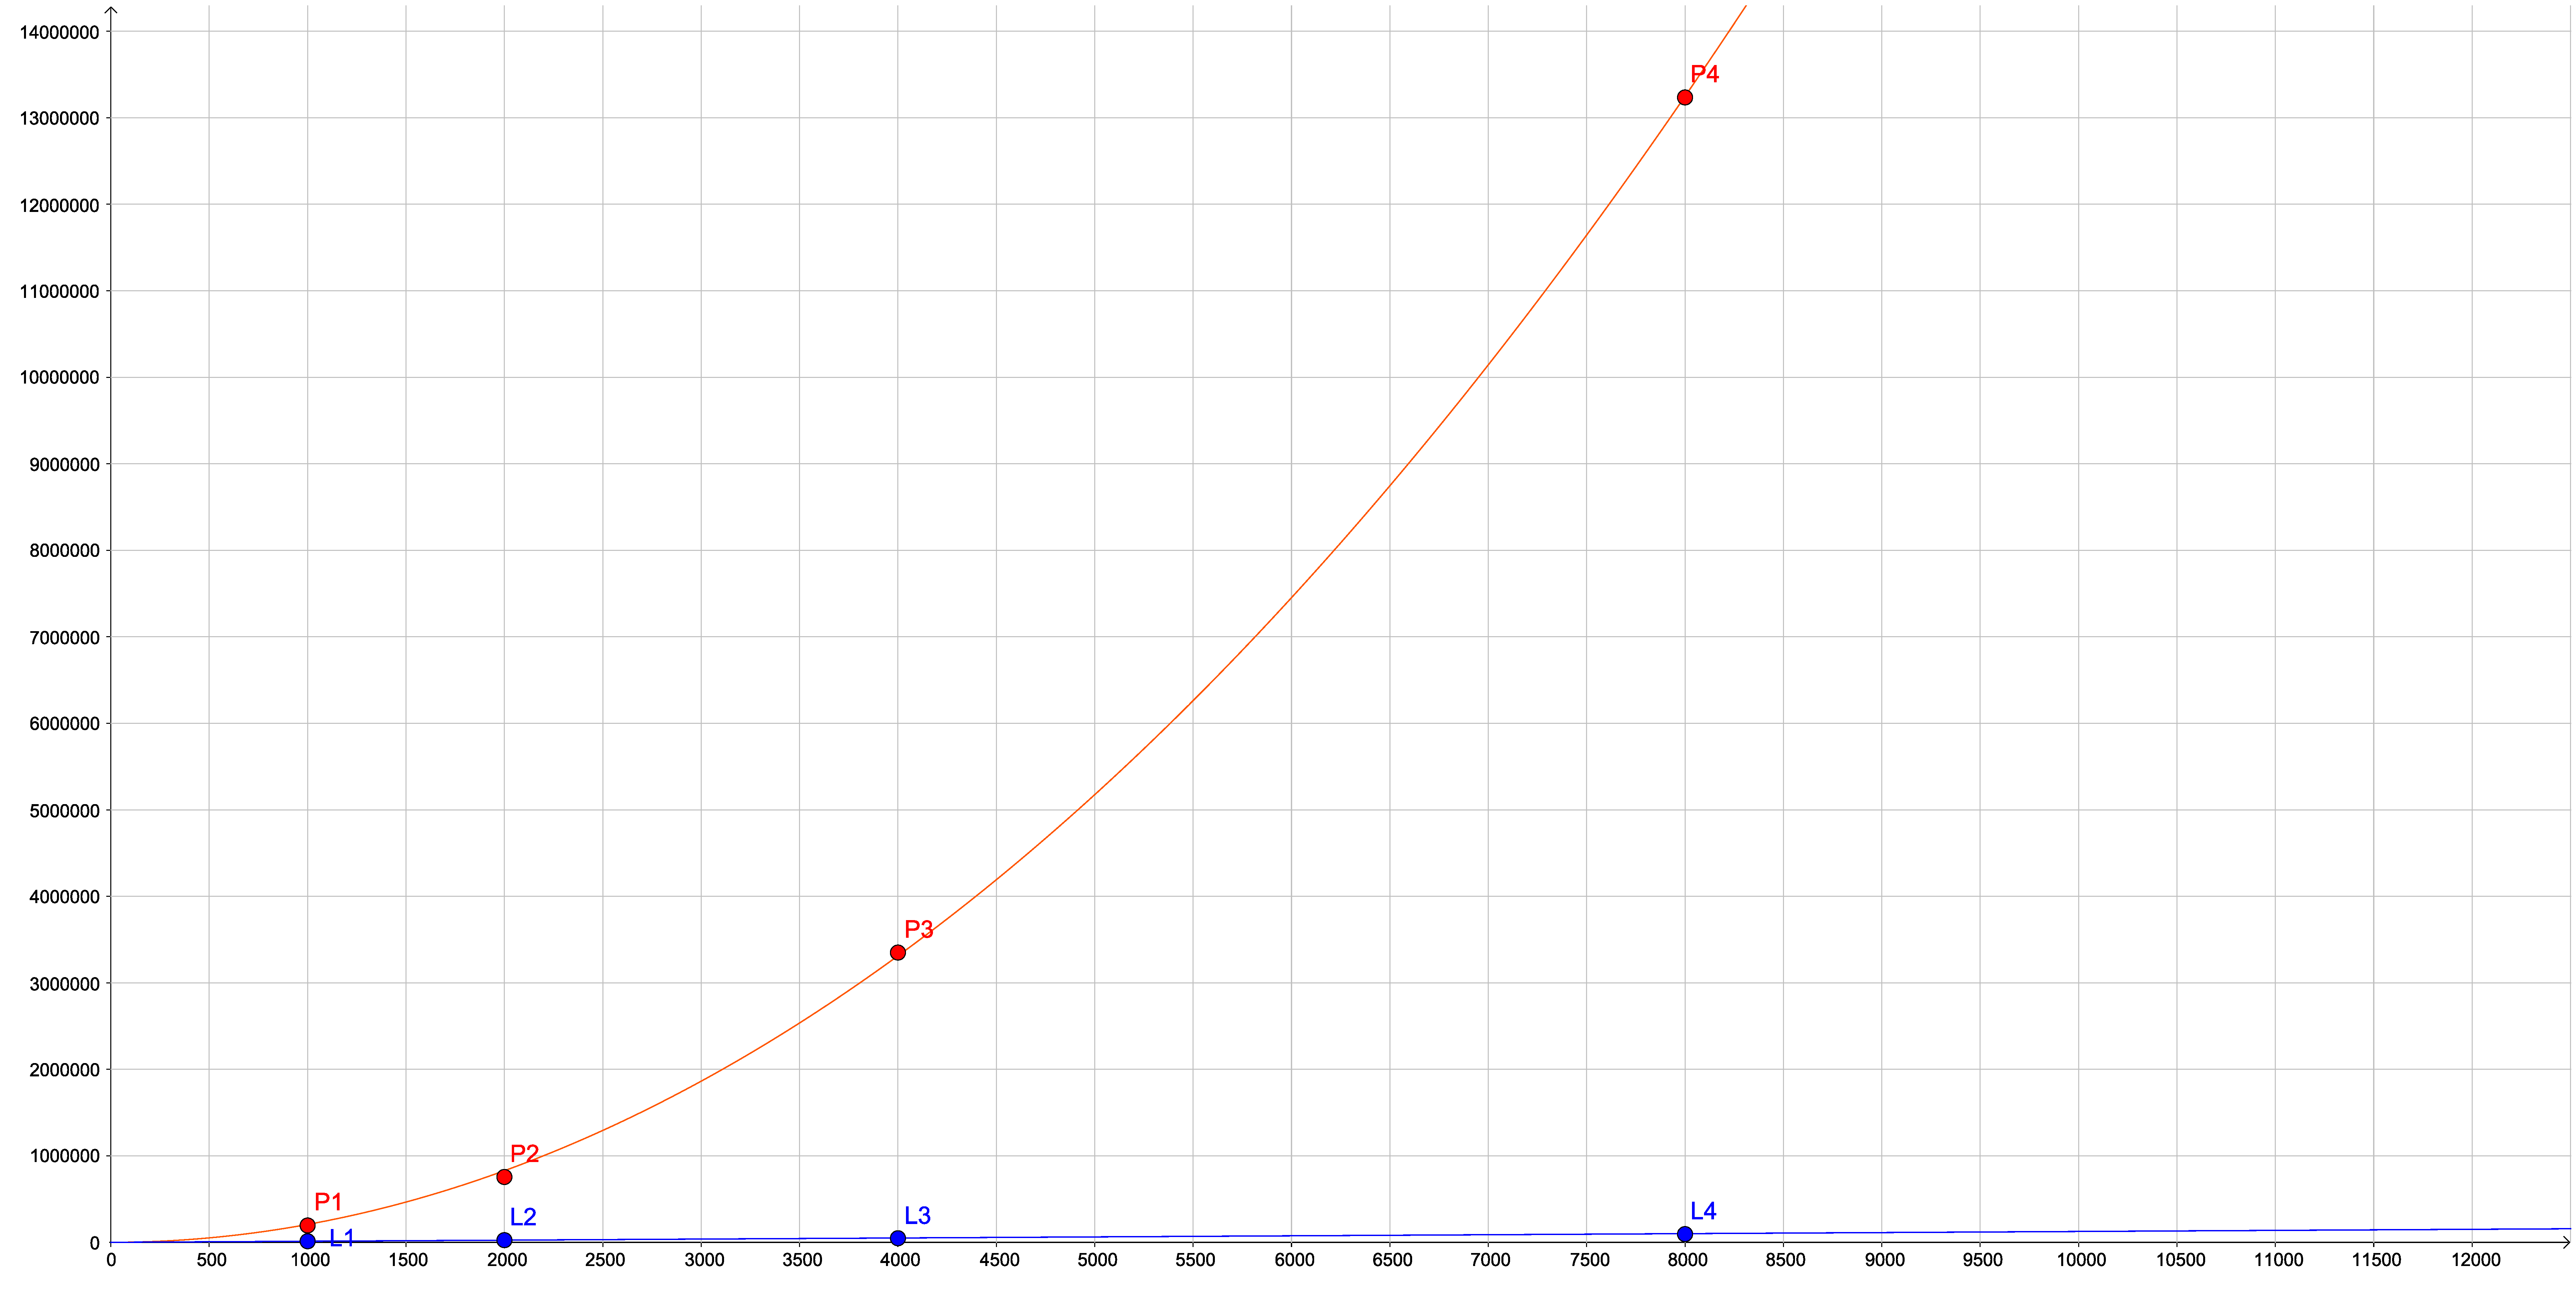
\includegraphics[width=40cm]{test}
\caption{Performance test}
\end{DoxyImage}
\hypertarget{index_thread_sec}{}\section{Parallelization}\label{index_thread_sec}
The following graph compares the Molecule-\/\+Updates per Second depending on the number of threads used. The configuration file used was setting-\/liquid.\+xml   
\begin{DoxyImage}
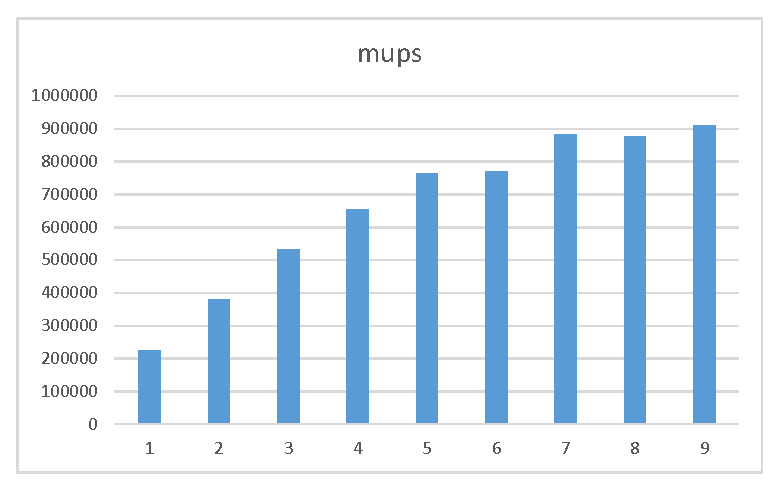
\includegraphics[width=40cm]{mups}
\caption{Performance test}
\end{DoxyImage}
 
\chapter{Namespace Index}
\section{Namespace List}
Here is a list of all namespaces with brief descriptions\+:\begin{DoxyCompactList}
\item\contentsline{section}{\hyperlink{namespaceoutputWriter}{output\+Writer} }{\pageref{namespaceoutputWriter}}{}
\item\contentsline{section}{\hyperlink{namespaceutils}{utils} }{\pageref{namespaceutils}}{}
\item\contentsline{section}{\hyperlink{namespacexml__schema}{xml\+\_\+schema} }{\pageref{namespacexml__schema}}{}
\item\contentsline{section}{\hyperlink{namespacexml__schema_1_1dom}{xml\+\_\+schema\+::dom} }{\pageref{namespacexml__schema_1_1dom}}{}
\end{DoxyCompactList}

\chapter{Hierarchical Index}
\section{Class Hierarchy}
This inheritance list is sorted roughly, but not completely, alphabetically\+:\begin{DoxyCompactList}
\item \contentsline{section}{output\+Writer\+:\+:C\+S\+V\+Writer}{\pageref{classoutputWriter_1_1CSVWriter}}{}
\item \contentsline{section}{File\+Reader}{\pageref{classFileReader}}{}
\item list\begin{DoxyCompactList}
\item \contentsline{section}{Data\+Array\+List\+\_\+t}{\pageref{classDataArrayList__t}}{}
\begin{DoxyCompactList}
\item \contentsline{section}{Data\+Array\+\_\+t}{\pageref{classDataArray__t}}{}
\end{DoxyCompactList}
\end{DoxyCompactList}
\item \contentsline{section}{Particle}{\pageref{classParticle}}{}
\item \contentsline{section}{Particle\+Container}{\pageref{classParticleContainer}}{}
\begin{DoxyCompactList}
\item \contentsline{section}{Linked\+Cells\+Container}{\pageref{classLinkedCellsContainer}}{}
\end{DoxyCompactList}
\item \contentsline{section}{Particle\+Type}{\pageref{classParticleType}}{}
\item simple\+\_\+type\begin{DoxyCompactList}
\item \contentsline{section}{Data\+Array\+List\+\_\+t}{\pageref{classDataArrayList__t}}{}
\end{DoxyCompactList}
\item string\begin{DoxyCompactList}
\item \contentsline{section}{type}{\pageref{classtype}}{}
\end{DoxyCompactList}
\item Test\+Fixture\begin{DoxyCompactList}
\item \contentsline{section}{Linked\+Container\+Test}{\pageref{classLinkedContainerTest}}{}
\item \contentsline{section}{Particle\+Container\+Test}{\pageref{classParticleContainerTest}}{}
\end{DoxyCompactList}
\item type\begin{DoxyCompactList}
\item \contentsline{section}{Cell\+Data}{\pageref{classCellData}}{}
\item \contentsline{section}{Cells}{\pageref{classCells}}{}
\item \contentsline{section}{cuboid\+\_\+t}{\pageref{classcuboid__t}}{}
\item \contentsline{section}{input\+\_\+t}{\pageref{classinput__t}}{}
\item \contentsline{section}{int\+\_\+vector\+\_\+t}{\pageref{classint__vector__t}}{}
\item \contentsline{section}{membrane\+\_\+t}{\pageref{classmembrane__t}}{}
\item \contentsline{section}{particletype\+\_\+t}{\pageref{classparticletype__t}}{}
\item \contentsline{section}{Piece\+Unstructured\+Grid\+\_\+t}{\pageref{classPieceUnstructuredGrid__t}}{}
\item \contentsline{section}{Point\+Data}{\pageref{classPointData}}{}
\item \contentsline{section}{Points}{\pageref{classPoints}}{}
\item \contentsline{section}{Poly\+Data\+\_\+t}{\pageref{classPolyData__t}}{}
\item \contentsline{section}{setting\+\_\+t}{\pageref{classsetting__t}}{}
\item \contentsline{section}{single\+\_\+t}{\pageref{classsingle__t}}{}
\item \contentsline{section}{sphere\+\_\+t}{\pageref{classsphere__t}}{}
\item \contentsline{section}{thermo\+\_\+t}{\pageref{classthermo__t}}{}
\item \contentsline{section}{thermo\+\_\+target\+\_\+t}{\pageref{classthermo__target__t}}{}
\item \contentsline{section}{Unstructured\+Grid\+\_\+t}{\pageref{classUnstructuredGrid__t}}{}
\item \contentsline{section}{vector\+\_\+t}{\pageref{classvector__t}}{}
\item \contentsline{section}{V\+T\+K\+File\+\_\+t}{\pageref{classVTKFile__t}}{}
\end{DoxyCompactList}
\item \contentsline{section}{utils\+:\+:Vector$<$ type, length $>$}{\pageref{classutils_1_1Vector}}{}
\item \contentsline{section}{utils\+:\+:Vector$<$ double, 3 $>$}{\pageref{classutils_1_1Vector}}{}
\item \contentsline{section}{utils\+:\+:Vector$<$ int, 6 $>$}{\pageref{classutils_1_1Vector}}{}
\item \contentsline{section}{output\+Writer\+:\+:V\+T\+K\+Writer}{\pageref{classoutputWriter_1_1VTKWriter}}{}
\item \contentsline{section}{output\+Writer\+:\+:X\+M\+L\+Writer}{\pageref{classoutputWriter_1_1XMLWriter}}{}
\item \contentsline{section}{output\+Writer\+:\+:X\+Y\+Z\+Writer}{\pageref{classoutputWriter_1_1XYZWriter}}{}
\end{DoxyCompactList}

\chapter{Class Index}
\section{Class List}
Here are the classes, structs, unions and interfaces with brief descriptions\+:\begin{DoxyCompactList}
\item\contentsline{section}{\hyperlink{classCellData}{Cell\+Data} }{\pageref{classCellData}}{}
\item\contentsline{section}{\hyperlink{classCells}{Cells} }{\pageref{classCells}}{}
\item\contentsline{section}{\hyperlink{classoutputWriter_1_1CSVWriter}{output\+Writer\+::\+C\+S\+V\+Writer} }{\pageref{classoutputWriter_1_1CSVWriter}}{}
\item\contentsline{section}{\hyperlink{classcuboid__t}{cuboid\+\_\+t} }{\pageref{classcuboid__t}}{}
\item\contentsline{section}{\hyperlink{classDataArray__t}{Data\+Array\+\_\+t} }{\pageref{classDataArray__t}}{}
\item\contentsline{section}{\hyperlink{classDataArrayList__t}{Data\+Array\+List\+\_\+t} }{\pageref{classDataArrayList__t}}{}
\item\contentsline{section}{\hyperlink{classFileReader}{File\+Reader} }{\pageref{classFileReader}}{}
\item\contentsline{section}{\hyperlink{classinput__t}{input\+\_\+t} }{\pageref{classinput__t}}{}
\item\contentsline{section}{\hyperlink{classint__vector__t}{int\+\_\+vector\+\_\+t} }{\pageref{classint__vector__t}}{}
\item\contentsline{section}{\hyperlink{classLinkedCellsContainer}{Linked\+Cells\+Container} \\*Class to hold cells containing a set of particles }{\pageref{classLinkedCellsContainer}}{}
\item\contentsline{section}{\hyperlink{classLinkedContainerTest}{Linked\+Container\+Test} \\*Test\+Suite for Linked\+Container }{\pageref{classLinkedContainerTest}}{}
\item\contentsline{section}{\hyperlink{classmembrane__t}{membrane\+\_\+t} }{\pageref{classmembrane__t}}{}
\item\contentsline{section}{\hyperlink{classParticle}{Particle} }{\pageref{classParticle}}{}
\item\contentsline{section}{\hyperlink{classParticleContainer}{Particle\+Container} \\*Class to hold a set of particles }{\pageref{classParticleContainer}}{}
\item\contentsline{section}{\hyperlink{classParticleContainerTest}{Particle\+Container\+Test} \\*Test\+Suite for \hyperlink{classParticleContainer}{Particle\+Container} }{\pageref{classParticleContainerTest}}{}
\item\contentsline{section}{\hyperlink{classParticleType}{Particle\+Type} \\*Class that defines properties of a particle type }{\pageref{classParticleType}}{}
\item\contentsline{section}{\hyperlink{classparticletype__t}{particletype\+\_\+t} }{\pageref{classparticletype__t}}{}
\item\contentsline{section}{\hyperlink{classPieceUnstructuredGrid__t}{Piece\+Unstructured\+Grid\+\_\+t} }{\pageref{classPieceUnstructuredGrid__t}}{}
\item\contentsline{section}{\hyperlink{classPointData}{Point\+Data} }{\pageref{classPointData}}{}
\item\contentsline{section}{\hyperlink{classPoints}{Points} }{\pageref{classPoints}}{}
\item\contentsline{section}{\hyperlink{classPolyData__t}{Poly\+Data\+\_\+t} }{\pageref{classPolyData__t}}{}
\item\contentsline{section}{\hyperlink{classsetting__t}{setting\+\_\+t} }{\pageref{classsetting__t}}{}
\item\contentsline{section}{\hyperlink{classsingle__t}{single\+\_\+t} }{\pageref{classsingle__t}}{}
\item\contentsline{section}{\hyperlink{classsphere__t}{sphere\+\_\+t} }{\pageref{classsphere__t}}{}
\item\contentsline{section}{\hyperlink{classthermo__t}{thermo\+\_\+t} }{\pageref{classthermo__t}}{}
\item\contentsline{section}{\hyperlink{classthermo__target__t}{thermo\+\_\+target\+\_\+t} }{\pageref{classthermo__target__t}}{}
\item\contentsline{section}{\hyperlink{classtype}{type} }{\pageref{classtype}}{}
\item\contentsline{section}{\hyperlink{classUnstructuredGrid__t}{Unstructured\+Grid\+\_\+t} }{\pageref{classUnstructuredGrid__t}}{}
\item\contentsline{section}{\hyperlink{classutils_1_1Vector}{utils\+::\+Vector$<$ type, length $>$} }{\pageref{classutils_1_1Vector}}{}
\item\contentsline{section}{\hyperlink{classvector__t}{vector\+\_\+t} }{\pageref{classvector__t}}{}
\item\contentsline{section}{\hyperlink{classVTKFile__t}{V\+T\+K\+File\+\_\+t} }{\pageref{classVTKFile__t}}{}
\item\contentsline{section}{\hyperlink{classoutputWriter_1_1VTKWriter}{output\+Writer\+::\+V\+T\+K\+Writer} }{\pageref{classoutputWriter_1_1VTKWriter}}{}
\item\contentsline{section}{\hyperlink{classoutputWriter_1_1XMLWriter}{output\+Writer\+::\+X\+M\+L\+Writer} }{\pageref{classoutputWriter_1_1XMLWriter}}{}
\item\contentsline{section}{\hyperlink{classoutputWriter_1_1XYZWriter}{output\+Writer\+::\+X\+Y\+Z\+Writer} }{\pageref{classoutputWriter_1_1XYZWriter}}{}
\end{DoxyCompactList}

\chapter{File Index}
\section{File List}
Here is a list of all files with brief descriptions\+:\begin{DoxyCompactList}
\item\contentsline{section}{src/\hyperlink{LinkedCellsContainer_8cpp}{Linked\+Cells\+Container.\+cpp} }{\pageref{LinkedCellsContainer_8cpp}}{}
\item\contentsline{section}{src/\hyperlink{LinkedCellsContainer_8h}{Linked\+Cells\+Container.\+h} }{\pageref{LinkedCellsContainer_8h}}{}
\item\contentsline{section}{src/\hyperlink{MaxwellBoltzmannDistribution_8cpp}{Maxwell\+Boltzmann\+Distribution.\+cpp} }{\pageref{MaxwellBoltzmannDistribution_8cpp}}{}
\item\contentsline{section}{src/\hyperlink{MaxwellBoltzmannDistribution_8h}{Maxwell\+Boltzmann\+Distribution.\+h} }{\pageref{MaxwellBoltzmannDistribution_8h}}{}
\item\contentsline{section}{src/\hyperlink{MolSim_8cpp}{Mol\+Sim.\+cpp} }{\pageref{MolSim_8cpp}}{}
\item\contentsline{section}{src/\hyperlink{Particle_8cpp}{Particle.\+cpp} }{\pageref{Particle_8cpp}}{}
\item\contentsline{section}{src/\hyperlink{Particle_8h}{Particle.\+h} }{\pageref{Particle_8h}}{}
\item\contentsline{section}{src/\hyperlink{ParticleContainer_8cpp}{Particle\+Container.\+cpp} }{\pageref{ParticleContainer_8cpp}}{}
\item\contentsline{section}{src/\hyperlink{ParticleContainer_8h}{Particle\+Container.\+h} }{\pageref{ParticleContainer_8h}}{}
\item\contentsline{section}{src/\hyperlink{ParticleType_8cpp}{Particle\+Type.\+cpp} }{\pageref{ParticleType_8cpp}}{}
\item\contentsline{section}{src/\hyperlink{ParticleType_8h}{Particle\+Type.\+h} }{\pageref{ParticleType_8h}}{}
\item\contentsline{section}{src/input/\hyperlink{FileReader_8cpp}{File\+Reader.\+cpp} }{\pageref{FileReader_8cpp}}{}
\item\contentsline{section}{src/input/\hyperlink{FileReader_8h}{File\+Reader.\+h} }{\pageref{FileReader_8h}}{}
\item\contentsline{section}{src/input/\hyperlink{particle__input_8cpp}{particle\+\_\+input.\+cpp} }{\pageref{particle__input_8cpp}}{}
\item\contentsline{section}{src/input/\hyperlink{particle__input_8h}{particle\+\_\+input.\+h} }{\pageref{particle__input_8h}}{}
\item\contentsline{section}{src/output\+Writer/\hyperlink{CSVWriter_8cpp}{C\+S\+V\+Writer.\+cpp} }{\pageref{CSVWriter_8cpp}}{}
\item\contentsline{section}{src/output\+Writer/\hyperlink{CSVWriter_8h}{C\+S\+V\+Writer.\+h} }{\pageref{CSVWriter_8h}}{}
\item\contentsline{section}{src/output\+Writer/\hyperlink{vtk-unstructured_8cpp}{vtk-\/unstructured.\+cpp} }{\pageref{vtk-unstructured_8cpp}}{}
\item\contentsline{section}{src/output\+Writer/\hyperlink{vtk-unstructured_8h}{vtk-\/unstructured.\+h} }{\pageref{vtk-unstructured_8h}}{}
\item\contentsline{section}{src/output\+Writer/\hyperlink{VTKWriter_8cpp}{V\+T\+K\+Writer.\+cpp} }{\pageref{VTKWriter_8cpp}}{}
\item\contentsline{section}{src/output\+Writer/\hyperlink{VTKWriter_8h}{V\+T\+K\+Writer.\+h} }{\pageref{VTKWriter_8h}}{}
\item\contentsline{section}{src/output\+Writer/\hyperlink{XMLWriter_8cpp}{X\+M\+L\+Writer.\+cpp} }{\pageref{XMLWriter_8cpp}}{}
\item\contentsline{section}{src/output\+Writer/\hyperlink{XMLWriter_8h}{X\+M\+L\+Writer.\+h} }{\pageref{XMLWriter_8h}}{}
\item\contentsline{section}{src/output\+Writer/\hyperlink{XYZWriter_8cpp}{X\+Y\+Z\+Writer.\+cpp} }{\pageref{XYZWriter_8cpp}}{}
\item\contentsline{section}{src/output\+Writer/\hyperlink{XYZWriter_8h}{X\+Y\+Z\+Writer.\+h} }{\pageref{XYZWriter_8h}}{}
\item\contentsline{section}{src/setting/\hyperlink{setting_8cpp}{setting.\+cpp} }{\pageref{setting_8cpp}}{}
\item\contentsline{section}{src/setting/\hyperlink{setting_8h}{setting.\+h} }{\pageref{setting_8h}}{}
\item\contentsline{section}{src/tests/\hyperlink{LinkedContainerTest_8cpp}{Linked\+Container\+Test.\+cpp} }{\pageref{LinkedContainerTest_8cpp}}{}
\item\contentsline{section}{src/tests/\hyperlink{LinkedContainerTest_8h}{Linked\+Container\+Test.\+h} }{\pageref{LinkedContainerTest_8h}}{}
\item\contentsline{section}{src/tests/\hyperlink{ParticleContainerTest_8cpp}{Particle\+Container\+Test.\+cpp} }{\pageref{ParticleContainerTest_8cpp}}{}
\item\contentsline{section}{src/tests/\hyperlink{ParticleContainerTest_8h}{Particle\+Container\+Test.\+h} }{\pageref{ParticleContainerTest_8h}}{}
\item\contentsline{section}{src/utils/\hyperlink{Vector_8h}{Vector.\+h} }{\pageref{Vector_8h}}{}
\end{DoxyCompactList}

\chapter{Namespace Documentation}
\hypertarget{namespaceoutputWriter}{}\section{output\+Writer Namespace Reference}
\label{namespaceoutputWriter}\index{output\+Writer@{output\+Writer}}
\subsection*{Classes}
\begin{DoxyCompactItemize}
\item 
class \hyperlink{classoutputWriter_1_1CSVWriter}{C\+S\+V\+Writer}
\item 
class \hyperlink{classoutputWriter_1_1VTKWriter}{V\+T\+K\+Writer}
\item 
class \hyperlink{classoutputWriter_1_1XMLWriter}{X\+M\+L\+Writer}
\item 
class \hyperlink{classoutputWriter_1_1XYZWriter}{X\+Y\+Z\+Writer}
\end{DoxyCompactItemize}

\hypertarget{namespaceutils}{}\section{utils Namespace Reference}
\label{namespaceutils}\index{utils@{utils}}
\subsection*{Classes}
\begin{DoxyCompactItemize}
\item 
class \hyperlink{classutils_1_1Vector}{Vector}
\end{DoxyCompactItemize}

\hypertarget{namespacexml__schema}{}\section{xml\+\_\+schema Namespace Reference}
\label{namespacexml__schema}\index{xml\+\_\+schema@{xml\+\_\+schema}}
\subsection*{Namespaces}
\begin{DoxyCompactItemize}
\item 
 \hyperlink{namespacexml__schema_1_1dom}{dom}
\end{DoxyCompactItemize}
\subsection*{Typedefs}
\begin{DoxyCompactItemize}
\item 
typedef \+::xsd\+::cxx\+::tree\+::type \hyperlink{namespacexml__schema_a4bf7f144ce936a6a393de26f4cb707f0}{type}
\item 
typedef \+::xsd\+::cxx\+::tree\+::simple\+\_\+type$<$ char, \hyperlink{namespacexml__schema_a4bf7f144ce936a6a393de26f4cb707f0}{type} $>$ \hyperlink{namespacexml__schema_a2ee8a034145ffa154d46910b41892495}{simple\+\_\+type}
\item 
typedef \+::xsd\+::cxx\+::tree\+::type \hyperlink{namespacexml__schema_ada9aa30dc722e93ee2ed7243085402a5}{container}
\item 
typedef signed char \hyperlink{namespacexml__schema_a2a462724b41fb68016d13b34f9a84b7d}{byte}
\item 
typedef unsigned char \hyperlink{namespacexml__schema_a876b68656d976c6343512f3d44fe8ca2}{unsigned\+\_\+byte}
\item 
typedef short \hyperlink{namespacexml__schema_a705720c1fed1575ccdcfd21cb7ab39ab}{short\+\_\+}
\item 
typedef unsigned short \hyperlink{namespacexml__schema_a7fc7b4a846c512c370346e15dfdcecaa}{unsigned\+\_\+short}
\item 
typedef int \hyperlink{namespacexml__schema_acfa24ac68e1a188e7f44c36f7a158bf4}{int\+\_\+}
\item 
typedef unsigned int \hyperlink{namespacexml__schema_a85ca3205d8af287e149aac54535f57e7}{unsigned\+\_\+int}
\item 
typedef long long \hyperlink{namespacexml__schema_a1d78aacee49e26cb7a69d5aa97df1268}{long\+\_\+}
\item 
typedef unsigned long long \hyperlink{namespacexml__schema_a4413fbcf4c65ffc7aaafe465d72fcb33}{unsigned\+\_\+long}
\item 
typedef long long \hyperlink{namespacexml__schema_aaaea7c8ce4dfbe26cc52c91c29c97b7c}{integer}
\item 
typedef long long \hyperlink{namespacexml__schema_a3de6073e510eb8edd71ddc6e0256e2f9}{non\+\_\+positive\+\_\+integer}
\item 
typedef unsigned long long \hyperlink{namespacexml__schema_af42ef5911d65f41a0a03598b056f05aa}{non\+\_\+negative\+\_\+integer}
\item 
typedef unsigned long long \hyperlink{namespacexml__schema_abe9d639a15a121d2868ae2f9c974ca24}{positive\+\_\+integer}
\item 
typedef long long \hyperlink{namespacexml__schema_acf9528a84381d07f2802785c947bf441}{negative\+\_\+integer}
\item 
typedef bool \hyperlink{namespacexml__schema_ae5ada4ec9c54b51765c3e4c0e9631bba}{boolean}
\item 
typedef float \hyperlink{namespacexml__schema_ad7e04ab17bba0b3fdde43fb79ef6ed87}{float\+\_\+}
\item 
typedef double \hyperlink{namespacexml__schema_aac2d3d3483d3a20e8d96d2e8e5b3a470}{double\+\_\+}
\item 
typedef double \hyperlink{namespacexml__schema_a69bfaf24f63a8c18ebd8e21db6b343df}{decimal}
\item 
typedef \+::xsd\+::cxx\+::tree\+::string$<$ char, \hyperlink{namespacexml__schema_a2ee8a034145ffa154d46910b41892495}{simple\+\_\+type} $>$ \hyperlink{namespacexml__schema_ac0cec83a330f0024e4e318b3deac5104}{string}
\item 
typedef \+::xsd\+::cxx\+::tree\+::normalized\+\_\+string$<$ char, \hyperlink{namespacexml__schema_ac0cec83a330f0024e4e318b3deac5104}{string} $>$ \hyperlink{namespacexml__schema_a72078e45c15d8879c64071dea056f60c}{normalized\+\_\+string}
\item 
typedef \+::xsd\+::cxx\+::tree\+::token$<$ char, \hyperlink{namespacexml__schema_a72078e45c15d8879c64071dea056f60c}{normalized\+\_\+string} $>$ \hyperlink{namespacexml__schema_aac8666db04b41e8b19afa60d8ecb1e89}{token}
\item 
typedef \+::xsd\+::cxx\+::tree\+::name$<$ char, \hyperlink{namespacexml__schema_aac8666db04b41e8b19afa60d8ecb1e89}{token} $>$ \hyperlink{namespacexml__schema_a2f1617231643eded4c3b9aa5f1ed6c08}{name}
\item 
typedef \+::xsd\+::cxx\+::tree\+::nmtoken$<$ char, \hyperlink{namespacexml__schema_aac8666db04b41e8b19afa60d8ecb1e89}{token} $>$ \hyperlink{namespacexml__schema_af60189e21a69b126898eb625992ff730}{nmtoken}
\item 
typedef \+::xsd\+::cxx\+::tree\+::nmtokens$<$ char, \hyperlink{namespacexml__schema_a2ee8a034145ffa154d46910b41892495}{simple\+\_\+type}, \hyperlink{namespacexml__schema_af60189e21a69b126898eb625992ff730}{nmtoken} $>$ \hyperlink{namespacexml__schema_ab2ece9a172d690c8276a27fa696a3b43}{nmtokens}
\item 
typedef \+::xsd\+::cxx\+::tree\+::ncname$<$ char, \hyperlink{namespacexml__schema_a2f1617231643eded4c3b9aa5f1ed6c08}{name} $>$ \hyperlink{namespacexml__schema_adb64d7469eb27804ae649fbaccba54d6}{ncname}
\item 
typedef \+::xsd\+::cxx\+::tree\+::language$<$ char, \hyperlink{namespacexml__schema_aac8666db04b41e8b19afa60d8ecb1e89}{token} $>$ \hyperlink{namespacexml__schema_a9ccaf8d8efb41ea5331f512f381fc6ce}{language}
\item 
typedef \+::xsd\+::cxx\+::tree\+::id$<$ char, \hyperlink{namespacexml__schema_adb64d7469eb27804ae649fbaccba54d6}{ncname} $>$ \hyperlink{namespacexml__schema_a551698f0c4c57e5e194dc1f2892da3ef}{id}
\item 
typedef \+::xsd\+::cxx\+::tree\+::idref$<$ char, \hyperlink{namespacexml__schema_adb64d7469eb27804ae649fbaccba54d6}{ncname}, \hyperlink{namespacexml__schema_a4bf7f144ce936a6a393de26f4cb707f0}{type} $>$ \hyperlink{namespacexml__schema_a50fe7403f3e6be3634976c84c1ea1f8c}{idref}
\item 
typedef \+::xsd\+::cxx\+::tree\+::idrefs$<$ char, \hyperlink{namespacexml__schema_a2ee8a034145ffa154d46910b41892495}{simple\+\_\+type}, \hyperlink{namespacexml__schema_a50fe7403f3e6be3634976c84c1ea1f8c}{idref} $>$ \hyperlink{namespacexml__schema_aac27fe5af9a5b2ee009fd3c9abe3abe9}{idrefs}
\item 
typedef \+::xsd\+::cxx\+::tree\+::uri$<$ char, \hyperlink{namespacexml__schema_a2ee8a034145ffa154d46910b41892495}{simple\+\_\+type} $>$ \hyperlink{namespacexml__schema_aad28b7e5769e04950db7f4bd15c163be}{uri}
\item 
typedef \+::xsd\+::cxx\+::tree\+::qname$<$ char, \hyperlink{namespacexml__schema_a2ee8a034145ffa154d46910b41892495}{simple\+\_\+type}, \hyperlink{namespacexml__schema_aad28b7e5769e04950db7f4bd15c163be}{uri}, \hyperlink{namespacexml__schema_adb64d7469eb27804ae649fbaccba54d6}{ncname} $>$ \hyperlink{namespacexml__schema_a5343b1a86a36b809f1acf953a2497af2}{qname}
\item 
typedef \+::xsd\+::cxx\+::tree\+::buffer$<$ char $>$ \hyperlink{namespacexml__schema_a3a1af5d598f84fcd6707cc9f84880533}{buffer}
\item 
typedef \+::xsd\+::cxx\+::tree\+::base64\+\_\+binary$<$ char, \hyperlink{namespacexml__schema_a2ee8a034145ffa154d46910b41892495}{simple\+\_\+type} $>$ \hyperlink{namespacexml__schema_a6a44de5a5883b8a6377178c988a87b93}{base64\+\_\+binary}
\item 
typedef \+::xsd\+::cxx\+::tree\+::hex\+\_\+binary$<$ char, \hyperlink{namespacexml__schema_a2ee8a034145ffa154d46910b41892495}{simple\+\_\+type} $>$ \hyperlink{namespacexml__schema_ac9db22d87610e02355669749770fac89}{hex\+\_\+binary}
\item 
typedef \+::xsd\+::cxx\+::tree\+::time\+\_\+zone \hyperlink{namespacexml__schema_ab32f228c8863c36bf48dbb7356c50c0e}{time\+\_\+zone}
\item 
typedef \+::xsd\+::cxx\+::tree\+::date$<$ char, \hyperlink{namespacexml__schema_a2ee8a034145ffa154d46910b41892495}{simple\+\_\+type} $>$ \hyperlink{namespacexml__schema_abc702b2b5f66618b0fdbbbe484492b4d}{date}
\item 
typedef \+::xsd\+::cxx\+::tree\+::date\+\_\+time$<$ char, \hyperlink{namespacexml__schema_a2ee8a034145ffa154d46910b41892495}{simple\+\_\+type} $>$ \hyperlink{namespacexml__schema_a94af98c4870fb2715706678639c97224}{date\+\_\+time}
\item 
typedef \+::xsd\+::cxx\+::tree\+::duration$<$ char, \hyperlink{namespacexml__schema_a2ee8a034145ffa154d46910b41892495}{simple\+\_\+type} $>$ \hyperlink{namespacexml__schema_a1acfdda85b50d50b1718ab6917a8f993}{duration}
\item 
typedef \+::xsd\+::cxx\+::tree\+::gday$<$ char, \hyperlink{namespacexml__schema_a2ee8a034145ffa154d46910b41892495}{simple\+\_\+type} $>$ \hyperlink{namespacexml__schema_a80cbdd05209953df8c443ba8d81d4c25}{gday}
\item 
typedef \+::xsd\+::cxx\+::tree\+::gmonth$<$ char, \hyperlink{namespacexml__schema_a2ee8a034145ffa154d46910b41892495}{simple\+\_\+type} $>$ \hyperlink{namespacexml__schema_afe97b9ae1d131c601ce16f8bb4cdc022}{gmonth}
\item 
typedef \+::xsd\+::cxx\+::tree\+::gmonth\+\_\+day$<$ char, \hyperlink{namespacexml__schema_a2ee8a034145ffa154d46910b41892495}{simple\+\_\+type} $>$ \hyperlink{namespacexml__schema_a61e87eff200c80a4fce76244d6d01296}{gmonth\+\_\+day}
\item 
typedef \+::xsd\+::cxx\+::tree\+::gyear$<$ char, \hyperlink{namespacexml__schema_a2ee8a034145ffa154d46910b41892495}{simple\+\_\+type} $>$ \hyperlink{namespacexml__schema_a180526e3ae3592e56a0037c1f2ec8e5b}{gyear}
\item 
typedef \+::xsd\+::cxx\+::tree\+::gyear\+\_\+month$<$ char, \hyperlink{namespacexml__schema_a2ee8a034145ffa154d46910b41892495}{simple\+\_\+type} $>$ \hyperlink{namespacexml__schema_a8da9330a638589b1ef456991753a2804}{gyear\+\_\+month}
\item 
typedef \+::xsd\+::cxx\+::tree\+::time$<$ char, \hyperlink{namespacexml__schema_a2ee8a034145ffa154d46910b41892495}{simple\+\_\+type} $>$ \hyperlink{namespacexml__schema_a59aaa57bb5452c1f6c6111f1501277d4}{time}
\item 
typedef \+::xsd\+::cxx\+::tree\+::entity$<$ char, \hyperlink{namespacexml__schema_adb64d7469eb27804ae649fbaccba54d6}{ncname} $>$ \hyperlink{namespacexml__schema_acbf59a94b42e0d01cdfc56b93465912a}{entity}
\item 
typedef \+::xsd\+::cxx\+::tree\+::entities$<$ char, \hyperlink{namespacexml__schema_a2ee8a034145ffa154d46910b41892495}{simple\+\_\+type}, \hyperlink{namespacexml__schema_acbf59a94b42e0d01cdfc56b93465912a}{entity} $>$ \hyperlink{namespacexml__schema_a27645dad916b7c154cfa441c84cfb8f8}{entities}
\item 
typedef \+::xsd\+::cxx\+::tree\+::content\+\_\+order \hyperlink{namespacexml__schema_ae41cf99d54d24cb0112ce5dc08726476}{content\+\_\+order}
\item 
typedef \+::xsd\+::cxx\+::xml\+::dom\+::namespace\+\_\+info$<$ char $>$ \hyperlink{namespacexml__schema_a3bd77dc3d8c54be1c5369ce1aa8abebf}{namespace\+\_\+info}
\item 
typedef \+::xsd\+::cxx\+::xml\+::dom\+::namespace\+\_\+infomap$<$ char $>$ \hyperlink{namespacexml__schema_a17712c8260e03226f0a9e4d21ab78f42}{namespace\+\_\+infomap}
\item 
typedef \+::xsd\+::cxx\+::tree\+::list\+\_\+stream$<$ char $>$ \hyperlink{namespacexml__schema_a840728106ddd08800e62729d4eddbbc8}{list\+\_\+stream}
\item 
typedef \+::xsd\+::cxx\+::tree\+::as\+\_\+double$<$ \hyperlink{namespacexml__schema_aac2d3d3483d3a20e8d96d2e8e5b3a470}{double\+\_\+} $>$ \hyperlink{namespacexml__schema_a87206181e6830ca01769709c8652e04f}{as\+\_\+double}
\item 
typedef \+::xsd\+::cxx\+::tree\+::as\+\_\+decimal$<$ \hyperlink{namespacexml__schema_a69bfaf24f63a8c18ebd8e21db6b343df}{decimal} $>$ \hyperlink{namespacexml__schema_a9f2da4453eff69ce95bda90bc5be140c}{as\+\_\+decimal}
\item 
typedef \+::xsd\+::cxx\+::tree\+::facet \hyperlink{namespacexml__schema_a93c13629796b43b1cc518145be3f5390}{facet}
\item 
typedef \+::xsd\+::cxx\+::tree\+::flags \hyperlink{namespacexml__schema_a0612287d030cb2732d31a45b258fdc87}{flags}
\item 
typedef \+::xsd\+::cxx\+::tree\+::properties$<$ char $>$ \hyperlink{namespacexml__schema_a1a8ebac679580b41baebd62c7d641c1d}{properties}
\item 
typedef \+::xsd\+::cxx\+::tree\+::severity \hyperlink{namespacexml__schema_a7d2d246dda9239f18f1866a1cdb4022e}{severity}
\item 
typedef \+::xsd\+::cxx\+::tree\+::error$<$ char $>$ \hyperlink{namespacexml__schema_a25204746dcf5a00a92e68d214a894b84}{error}
\item 
typedef \+::xsd\+::cxx\+::tree\+::diagnostics$<$ char $>$ \hyperlink{namespacexml__schema_a0d9a5a38c30964872464e338625301d8}{diagnostics}
\item 
typedef \+::xsd\+::cxx\+::tree\+::exception$<$ char $>$ \hyperlink{namespacexml__schema_a1e9265f27587f794fe1b02f5cefb447f}{exception}
\item 
typedef \+::xsd\+::cxx\+::tree\+::bounds$<$ char $>$ \hyperlink{namespacexml__schema_a0130942a2c58fd1fda434722d42ede1d}{bounds}
\item 
typedef \+::xsd\+::cxx\+::tree\+::duplicate\+\_\+id$<$ char $>$ \hyperlink{namespacexml__schema_a6dc417261c18af4fcce090133dd605f8}{duplicate\+\_\+id}
\item 
typedef \+::xsd\+::cxx\+::tree\+::parsing$<$ char $>$ \hyperlink{namespacexml__schema_afbb8ed049be1751901785a29a6d13942}{parsing}
\item 
typedef \+::xsd\+::cxx\+::tree\+::expected\+\_\+element$<$ char $>$ \hyperlink{namespacexml__schema_a8deca57d1e322d97eea32518a7237a49}{expected\+\_\+element}
\item 
typedef \+::xsd\+::cxx\+::tree\+::unexpected\+\_\+element$<$ char $>$ \hyperlink{namespacexml__schema_a381b3f3410f9f6ba1f44c5500d90345b}{unexpected\+\_\+element}
\item 
typedef \+::xsd\+::cxx\+::tree\+::expected\+\_\+attribute$<$ char $>$ \hyperlink{namespacexml__schema_af16d098ecb2b5ba96a0734aa34bd8a5b}{expected\+\_\+attribute}
\item 
typedef \+::xsd\+::cxx\+::tree\+::unexpected\+\_\+enumerator$<$ char $>$ \hyperlink{namespacexml__schema_a7601f5d15eeb816df6a0e1cb2b0f379b}{unexpected\+\_\+enumerator}
\item 
typedef \+::xsd\+::cxx\+::tree\+::expected\+\_\+text\+\_\+content$<$ char $>$ \hyperlink{namespacexml__schema_ad0938777db5685ea04372a964518e87b}{expected\+\_\+text\+\_\+content}
\item 
typedef \+::xsd\+::cxx\+::tree\+::no\+\_\+prefix\+\_\+mapping$<$ char $>$ \hyperlink{namespacexml__schema_a103914036487a85ba84743f0e65b1d96}{no\+\_\+prefix\+\_\+mapping}
\item 
typedef \+::xsd\+::cxx\+::tree\+::serialization$<$ char $>$ \hyperlink{namespacexml__schema_a4d53cd67b012b824d27e3248c1b2c4b1}{serialization}
\item 
typedef \+::xsd\+::cxx\+::xml\+::error\+\_\+handler$<$ char $>$ \hyperlink{namespacexml__schema_a0a5d9528e9175cedf199984a8bb64d62}{error\+\_\+handler}
\end{DoxyCompactItemize}


\subsection{Typedef Documentation}
\index{xml\+\_\+schema@{xml\+\_\+schema}!as\+\_\+decimal@{as\+\_\+decimal}}
\index{as\+\_\+decimal@{as\+\_\+decimal}!xml\+\_\+schema@{xml\+\_\+schema}}
\subsubsection[{\texorpdfstring{as\+\_\+decimal}{as_decimal}}]{\setlength{\rightskip}{0pt plus 5cm}typedef\+::xsd\+::cxx\+::tree\+::as\+\_\+decimal$<$ {\bf decimal} $>$ {\bf xml\+\_\+schema\+::as\+\_\+decimal}}\hypertarget{namespacexml__schema_a9f2da4453eff69ce95bda90bc5be140c}{}\label{namespacexml__schema_a9f2da4453eff69ce95bda90bc5be140c}
\index{xml\+\_\+schema@{xml\+\_\+schema}!as\+\_\+double@{as\+\_\+double}}
\index{as\+\_\+double@{as\+\_\+double}!xml\+\_\+schema@{xml\+\_\+schema}}
\subsubsection[{\texorpdfstring{as\+\_\+double}{as_double}}]{\setlength{\rightskip}{0pt plus 5cm}typedef\+::xsd\+::cxx\+::tree\+::as\+\_\+double$<$ {\bf double\+\_\+} $>$ {\bf xml\+\_\+schema\+::as\+\_\+double}}\hypertarget{namespacexml__schema_a87206181e6830ca01769709c8652e04f}{}\label{namespacexml__schema_a87206181e6830ca01769709c8652e04f}
\index{xml\+\_\+schema@{xml\+\_\+schema}!base64\+\_\+binary@{base64\+\_\+binary}}
\index{base64\+\_\+binary@{base64\+\_\+binary}!xml\+\_\+schema@{xml\+\_\+schema}}
\subsubsection[{\texorpdfstring{base64\+\_\+binary}{base64_binary}}]{\setlength{\rightskip}{0pt plus 5cm}typedef\+::xsd\+::cxx\+::tree\+::base64\+\_\+binary$<$ char, {\bf simple\+\_\+type} $>$ {\bf xml\+\_\+schema\+::base64\+\_\+binary}}\hypertarget{namespacexml__schema_a6a44de5a5883b8a6377178c988a87b93}{}\label{namespacexml__schema_a6a44de5a5883b8a6377178c988a87b93}
\index{xml\+\_\+schema@{xml\+\_\+schema}!boolean@{boolean}}
\index{boolean@{boolean}!xml\+\_\+schema@{xml\+\_\+schema}}
\subsubsection[{\texorpdfstring{boolean}{boolean}}]{\setlength{\rightskip}{0pt plus 5cm}typedef bool {\bf xml\+\_\+schema\+::boolean}}\hypertarget{namespacexml__schema_ae5ada4ec9c54b51765c3e4c0e9631bba}{}\label{namespacexml__schema_ae5ada4ec9c54b51765c3e4c0e9631bba}
\index{xml\+\_\+schema@{xml\+\_\+schema}!bounds@{bounds}}
\index{bounds@{bounds}!xml\+\_\+schema@{xml\+\_\+schema}}
\subsubsection[{\texorpdfstring{bounds}{bounds}}]{\setlength{\rightskip}{0pt plus 5cm}typedef\+::xsd\+::cxx\+::tree\+::bounds$<$ char $>$ {\bf xml\+\_\+schema\+::bounds}}\hypertarget{namespacexml__schema_a0130942a2c58fd1fda434722d42ede1d}{}\label{namespacexml__schema_a0130942a2c58fd1fda434722d42ede1d}
\index{xml\+\_\+schema@{xml\+\_\+schema}!buffer@{buffer}}
\index{buffer@{buffer}!xml\+\_\+schema@{xml\+\_\+schema}}
\subsubsection[{\texorpdfstring{buffer}{buffer}}]{\setlength{\rightskip}{0pt plus 5cm}typedef\+::xsd\+::cxx\+::tree\+::buffer$<$ char $>$ {\bf xml\+\_\+schema\+::buffer}}\hypertarget{namespacexml__schema_a3a1af5d598f84fcd6707cc9f84880533}{}\label{namespacexml__schema_a3a1af5d598f84fcd6707cc9f84880533}
\index{xml\+\_\+schema@{xml\+\_\+schema}!byte@{byte}}
\index{byte@{byte}!xml\+\_\+schema@{xml\+\_\+schema}}
\subsubsection[{\texorpdfstring{byte}{byte}}]{\setlength{\rightskip}{0pt plus 5cm}typedef signed char {\bf xml\+\_\+schema\+::byte}}\hypertarget{namespacexml__schema_a2a462724b41fb68016d13b34f9a84b7d}{}\label{namespacexml__schema_a2a462724b41fb68016d13b34f9a84b7d}
\index{xml\+\_\+schema@{xml\+\_\+schema}!container@{container}}
\index{container@{container}!xml\+\_\+schema@{xml\+\_\+schema}}
\subsubsection[{\texorpdfstring{container}{container}}]{\setlength{\rightskip}{0pt plus 5cm}typedef\+::xsd\+::cxx\+::tree\+::type {\bf xml\+\_\+schema\+::container}}\hypertarget{namespacexml__schema_ada9aa30dc722e93ee2ed7243085402a5}{}\label{namespacexml__schema_ada9aa30dc722e93ee2ed7243085402a5}
\index{xml\+\_\+schema@{xml\+\_\+schema}!content\+\_\+order@{content\+\_\+order}}
\index{content\+\_\+order@{content\+\_\+order}!xml\+\_\+schema@{xml\+\_\+schema}}
\subsubsection[{\texorpdfstring{content\+\_\+order}{content_order}}]{\setlength{\rightskip}{0pt plus 5cm}typedef\+::xsd\+::cxx\+::tree\+::content\+\_\+order {\bf xml\+\_\+schema\+::content\+\_\+order}}\hypertarget{namespacexml__schema_ae41cf99d54d24cb0112ce5dc08726476}{}\label{namespacexml__schema_ae41cf99d54d24cb0112ce5dc08726476}
\index{xml\+\_\+schema@{xml\+\_\+schema}!date@{date}}
\index{date@{date}!xml\+\_\+schema@{xml\+\_\+schema}}
\subsubsection[{\texorpdfstring{date}{date}}]{\setlength{\rightskip}{0pt plus 5cm}typedef\+::xsd\+::cxx\+::tree\+::date$<$ char, {\bf simple\+\_\+type} $>$ {\bf xml\+\_\+schema\+::date}}\hypertarget{namespacexml__schema_abc702b2b5f66618b0fdbbbe484492b4d}{}\label{namespacexml__schema_abc702b2b5f66618b0fdbbbe484492b4d}
\index{xml\+\_\+schema@{xml\+\_\+schema}!date\+\_\+time@{date\+\_\+time}}
\index{date\+\_\+time@{date\+\_\+time}!xml\+\_\+schema@{xml\+\_\+schema}}
\subsubsection[{\texorpdfstring{date\+\_\+time}{date_time}}]{\setlength{\rightskip}{0pt plus 5cm}typedef\+::xsd\+::cxx\+::tree\+::date\+\_\+time$<$ char, {\bf simple\+\_\+type} $>$ {\bf xml\+\_\+schema\+::date\+\_\+time}}\hypertarget{namespacexml__schema_a94af98c4870fb2715706678639c97224}{}\label{namespacexml__schema_a94af98c4870fb2715706678639c97224}
\index{xml\+\_\+schema@{xml\+\_\+schema}!decimal@{decimal}}
\index{decimal@{decimal}!xml\+\_\+schema@{xml\+\_\+schema}}
\subsubsection[{\texorpdfstring{decimal}{decimal}}]{\setlength{\rightskip}{0pt plus 5cm}typedef double {\bf xml\+\_\+schema\+::decimal}}\hypertarget{namespacexml__schema_a69bfaf24f63a8c18ebd8e21db6b343df}{}\label{namespacexml__schema_a69bfaf24f63a8c18ebd8e21db6b343df}
\index{xml\+\_\+schema@{xml\+\_\+schema}!diagnostics@{diagnostics}}
\index{diagnostics@{diagnostics}!xml\+\_\+schema@{xml\+\_\+schema}}
\subsubsection[{\texorpdfstring{diagnostics}{diagnostics}}]{\setlength{\rightskip}{0pt plus 5cm}typedef\+::xsd\+::cxx\+::tree\+::diagnostics$<$ char $>$ {\bf xml\+\_\+schema\+::diagnostics}}\hypertarget{namespacexml__schema_a0d9a5a38c30964872464e338625301d8}{}\label{namespacexml__schema_a0d9a5a38c30964872464e338625301d8}
\index{xml\+\_\+schema@{xml\+\_\+schema}!double\+\_\+@{double\+\_\+}}
\index{double\+\_\+@{double\+\_\+}!xml\+\_\+schema@{xml\+\_\+schema}}
\subsubsection[{\texorpdfstring{double\+\_\+}{double_}}]{\setlength{\rightskip}{0pt plus 5cm}typedef double {\bf xml\+\_\+schema\+::double\+\_\+}}\hypertarget{namespacexml__schema_aac2d3d3483d3a20e8d96d2e8e5b3a470}{}\label{namespacexml__schema_aac2d3d3483d3a20e8d96d2e8e5b3a470}
\index{xml\+\_\+schema@{xml\+\_\+schema}!duplicate\+\_\+id@{duplicate\+\_\+id}}
\index{duplicate\+\_\+id@{duplicate\+\_\+id}!xml\+\_\+schema@{xml\+\_\+schema}}
\subsubsection[{\texorpdfstring{duplicate\+\_\+id}{duplicate_id}}]{\setlength{\rightskip}{0pt plus 5cm}typedef\+::xsd\+::cxx\+::tree\+::duplicate\+\_\+id$<$ char $>$ {\bf xml\+\_\+schema\+::duplicate\+\_\+id}}\hypertarget{namespacexml__schema_a6dc417261c18af4fcce090133dd605f8}{}\label{namespacexml__schema_a6dc417261c18af4fcce090133dd605f8}
\index{xml\+\_\+schema@{xml\+\_\+schema}!duration@{duration}}
\index{duration@{duration}!xml\+\_\+schema@{xml\+\_\+schema}}
\subsubsection[{\texorpdfstring{duration}{duration}}]{\setlength{\rightskip}{0pt plus 5cm}typedef\+::xsd\+::cxx\+::tree\+::duration$<$ char, {\bf simple\+\_\+type} $>$ {\bf xml\+\_\+schema\+::duration}}\hypertarget{namespacexml__schema_a1acfdda85b50d50b1718ab6917a8f993}{}\label{namespacexml__schema_a1acfdda85b50d50b1718ab6917a8f993}
\index{xml\+\_\+schema@{xml\+\_\+schema}!entities@{entities}}
\index{entities@{entities}!xml\+\_\+schema@{xml\+\_\+schema}}
\subsubsection[{\texorpdfstring{entities}{entities}}]{\setlength{\rightskip}{0pt plus 5cm}typedef\+::xsd\+::cxx\+::tree\+::entities$<$ char, {\bf simple\+\_\+type}, {\bf entity} $>$ {\bf xml\+\_\+schema\+::entities}}\hypertarget{namespacexml__schema_a27645dad916b7c154cfa441c84cfb8f8}{}\label{namespacexml__schema_a27645dad916b7c154cfa441c84cfb8f8}
\index{xml\+\_\+schema@{xml\+\_\+schema}!entity@{entity}}
\index{entity@{entity}!xml\+\_\+schema@{xml\+\_\+schema}}
\subsubsection[{\texorpdfstring{entity}{entity}}]{\setlength{\rightskip}{0pt plus 5cm}typedef\+::xsd\+::cxx\+::tree\+::entity$<$ char, {\bf ncname} $>$ {\bf xml\+\_\+schema\+::entity}}\hypertarget{namespacexml__schema_acbf59a94b42e0d01cdfc56b93465912a}{}\label{namespacexml__schema_acbf59a94b42e0d01cdfc56b93465912a}
\index{xml\+\_\+schema@{xml\+\_\+schema}!error@{error}}
\index{error@{error}!xml\+\_\+schema@{xml\+\_\+schema}}
\subsubsection[{\texorpdfstring{error}{error}}]{\setlength{\rightskip}{0pt plus 5cm}typedef\+::xsd\+::cxx\+::tree\+::error$<$ char $>$ {\bf xml\+\_\+schema\+::error}}\hypertarget{namespacexml__schema_a25204746dcf5a00a92e68d214a894b84}{}\label{namespacexml__schema_a25204746dcf5a00a92e68d214a894b84}
\index{xml\+\_\+schema@{xml\+\_\+schema}!error\+\_\+handler@{error\+\_\+handler}}
\index{error\+\_\+handler@{error\+\_\+handler}!xml\+\_\+schema@{xml\+\_\+schema}}
\subsubsection[{\texorpdfstring{error\+\_\+handler}{error_handler}}]{\setlength{\rightskip}{0pt plus 5cm}typedef\+::xsd\+::cxx\+::xml\+::error\+\_\+handler$<$ char $>$ {\bf xml\+\_\+schema\+::error\+\_\+handler}}\hypertarget{namespacexml__schema_a0a5d9528e9175cedf199984a8bb64d62}{}\label{namespacexml__schema_a0a5d9528e9175cedf199984a8bb64d62}
\index{xml\+\_\+schema@{xml\+\_\+schema}!exception@{exception}}
\index{exception@{exception}!xml\+\_\+schema@{xml\+\_\+schema}}
\subsubsection[{\texorpdfstring{exception}{exception}}]{\setlength{\rightskip}{0pt plus 5cm}typedef\+::xsd\+::cxx\+::tree\+::exception$<$ char $>$ {\bf xml\+\_\+schema\+::exception}}\hypertarget{namespacexml__schema_a1e9265f27587f794fe1b02f5cefb447f}{}\label{namespacexml__schema_a1e9265f27587f794fe1b02f5cefb447f}
\index{xml\+\_\+schema@{xml\+\_\+schema}!expected\+\_\+attribute@{expected\+\_\+attribute}}
\index{expected\+\_\+attribute@{expected\+\_\+attribute}!xml\+\_\+schema@{xml\+\_\+schema}}
\subsubsection[{\texorpdfstring{expected\+\_\+attribute}{expected_attribute}}]{\setlength{\rightskip}{0pt plus 5cm}typedef\+::xsd\+::cxx\+::tree\+::expected\+\_\+attribute$<$ char $>$ {\bf xml\+\_\+schema\+::expected\+\_\+attribute}}\hypertarget{namespacexml__schema_af16d098ecb2b5ba96a0734aa34bd8a5b}{}\label{namespacexml__schema_af16d098ecb2b5ba96a0734aa34bd8a5b}
\index{xml\+\_\+schema@{xml\+\_\+schema}!expected\+\_\+element@{expected\+\_\+element}}
\index{expected\+\_\+element@{expected\+\_\+element}!xml\+\_\+schema@{xml\+\_\+schema}}
\subsubsection[{\texorpdfstring{expected\+\_\+element}{expected_element}}]{\setlength{\rightskip}{0pt plus 5cm}typedef\+::xsd\+::cxx\+::tree\+::expected\+\_\+element$<$ char $>$ {\bf xml\+\_\+schema\+::expected\+\_\+element}}\hypertarget{namespacexml__schema_a8deca57d1e322d97eea32518a7237a49}{}\label{namespacexml__schema_a8deca57d1e322d97eea32518a7237a49}
\index{xml\+\_\+schema@{xml\+\_\+schema}!expected\+\_\+text\+\_\+content@{expected\+\_\+text\+\_\+content}}
\index{expected\+\_\+text\+\_\+content@{expected\+\_\+text\+\_\+content}!xml\+\_\+schema@{xml\+\_\+schema}}
\subsubsection[{\texorpdfstring{expected\+\_\+text\+\_\+content}{expected_text_content}}]{\setlength{\rightskip}{0pt plus 5cm}typedef\+::xsd\+::cxx\+::tree\+::expected\+\_\+text\+\_\+content$<$ char $>$ {\bf xml\+\_\+schema\+::expected\+\_\+text\+\_\+content}}\hypertarget{namespacexml__schema_ad0938777db5685ea04372a964518e87b}{}\label{namespacexml__schema_ad0938777db5685ea04372a964518e87b}
\index{xml\+\_\+schema@{xml\+\_\+schema}!facet@{facet}}
\index{facet@{facet}!xml\+\_\+schema@{xml\+\_\+schema}}
\subsubsection[{\texorpdfstring{facet}{facet}}]{\setlength{\rightskip}{0pt plus 5cm}typedef\+::xsd\+::cxx\+::tree\+::facet {\bf xml\+\_\+schema\+::facet}}\hypertarget{namespacexml__schema_a93c13629796b43b1cc518145be3f5390}{}\label{namespacexml__schema_a93c13629796b43b1cc518145be3f5390}
\index{xml\+\_\+schema@{xml\+\_\+schema}!flags@{flags}}
\index{flags@{flags}!xml\+\_\+schema@{xml\+\_\+schema}}
\subsubsection[{\texorpdfstring{flags}{flags}}]{\setlength{\rightskip}{0pt plus 5cm}typedef\+::xsd\+::cxx\+::tree\+::flags {\bf xml\+\_\+schema\+::flags}}\hypertarget{namespacexml__schema_a0612287d030cb2732d31a45b258fdc87}{}\label{namespacexml__schema_a0612287d030cb2732d31a45b258fdc87}
\index{xml\+\_\+schema@{xml\+\_\+schema}!float\+\_\+@{float\+\_\+}}
\index{float\+\_\+@{float\+\_\+}!xml\+\_\+schema@{xml\+\_\+schema}}
\subsubsection[{\texorpdfstring{float\+\_\+}{float_}}]{\setlength{\rightskip}{0pt plus 5cm}typedef float {\bf xml\+\_\+schema\+::float\+\_\+}}\hypertarget{namespacexml__schema_ad7e04ab17bba0b3fdde43fb79ef6ed87}{}\label{namespacexml__schema_ad7e04ab17bba0b3fdde43fb79ef6ed87}
\index{xml\+\_\+schema@{xml\+\_\+schema}!gday@{gday}}
\index{gday@{gday}!xml\+\_\+schema@{xml\+\_\+schema}}
\subsubsection[{\texorpdfstring{gday}{gday}}]{\setlength{\rightskip}{0pt plus 5cm}typedef\+::xsd\+::cxx\+::tree\+::gday$<$ char, {\bf simple\+\_\+type} $>$ {\bf xml\+\_\+schema\+::gday}}\hypertarget{namespacexml__schema_a80cbdd05209953df8c443ba8d81d4c25}{}\label{namespacexml__schema_a80cbdd05209953df8c443ba8d81d4c25}
\index{xml\+\_\+schema@{xml\+\_\+schema}!gmonth@{gmonth}}
\index{gmonth@{gmonth}!xml\+\_\+schema@{xml\+\_\+schema}}
\subsubsection[{\texorpdfstring{gmonth}{gmonth}}]{\setlength{\rightskip}{0pt plus 5cm}typedef\+::xsd\+::cxx\+::tree\+::gmonth$<$ char, {\bf simple\+\_\+type} $>$ {\bf xml\+\_\+schema\+::gmonth}}\hypertarget{namespacexml__schema_afe97b9ae1d131c601ce16f8bb4cdc022}{}\label{namespacexml__schema_afe97b9ae1d131c601ce16f8bb4cdc022}
\index{xml\+\_\+schema@{xml\+\_\+schema}!gmonth\+\_\+day@{gmonth\+\_\+day}}
\index{gmonth\+\_\+day@{gmonth\+\_\+day}!xml\+\_\+schema@{xml\+\_\+schema}}
\subsubsection[{\texorpdfstring{gmonth\+\_\+day}{gmonth_day}}]{\setlength{\rightskip}{0pt plus 5cm}typedef\+::xsd\+::cxx\+::tree\+::gmonth\+\_\+day$<$ char, {\bf simple\+\_\+type} $>$ {\bf xml\+\_\+schema\+::gmonth\+\_\+day}}\hypertarget{namespacexml__schema_a61e87eff200c80a4fce76244d6d01296}{}\label{namespacexml__schema_a61e87eff200c80a4fce76244d6d01296}
\index{xml\+\_\+schema@{xml\+\_\+schema}!gyear@{gyear}}
\index{gyear@{gyear}!xml\+\_\+schema@{xml\+\_\+schema}}
\subsubsection[{\texorpdfstring{gyear}{gyear}}]{\setlength{\rightskip}{0pt plus 5cm}typedef\+::xsd\+::cxx\+::tree\+::gyear$<$ char, {\bf simple\+\_\+type} $>$ {\bf xml\+\_\+schema\+::gyear}}\hypertarget{namespacexml__schema_a180526e3ae3592e56a0037c1f2ec8e5b}{}\label{namespacexml__schema_a180526e3ae3592e56a0037c1f2ec8e5b}
\index{xml\+\_\+schema@{xml\+\_\+schema}!gyear\+\_\+month@{gyear\+\_\+month}}
\index{gyear\+\_\+month@{gyear\+\_\+month}!xml\+\_\+schema@{xml\+\_\+schema}}
\subsubsection[{\texorpdfstring{gyear\+\_\+month}{gyear_month}}]{\setlength{\rightskip}{0pt plus 5cm}typedef\+::xsd\+::cxx\+::tree\+::gyear\+\_\+month$<$ char, {\bf simple\+\_\+type} $>$ {\bf xml\+\_\+schema\+::gyear\+\_\+month}}\hypertarget{namespacexml__schema_a8da9330a638589b1ef456991753a2804}{}\label{namespacexml__schema_a8da9330a638589b1ef456991753a2804}
\index{xml\+\_\+schema@{xml\+\_\+schema}!hex\+\_\+binary@{hex\+\_\+binary}}
\index{hex\+\_\+binary@{hex\+\_\+binary}!xml\+\_\+schema@{xml\+\_\+schema}}
\subsubsection[{\texorpdfstring{hex\+\_\+binary}{hex_binary}}]{\setlength{\rightskip}{0pt plus 5cm}typedef\+::xsd\+::cxx\+::tree\+::hex\+\_\+binary$<$ char, {\bf simple\+\_\+type} $>$ {\bf xml\+\_\+schema\+::hex\+\_\+binary}}\hypertarget{namespacexml__schema_ac9db22d87610e02355669749770fac89}{}\label{namespacexml__schema_ac9db22d87610e02355669749770fac89}
\index{xml\+\_\+schema@{xml\+\_\+schema}!id@{id}}
\index{id@{id}!xml\+\_\+schema@{xml\+\_\+schema}}
\subsubsection[{\texorpdfstring{id}{id}}]{\setlength{\rightskip}{0pt plus 5cm}typedef\+::xsd\+::cxx\+::tree\+::id$<$ char, {\bf ncname} $>$ {\bf xml\+\_\+schema\+::id}}\hypertarget{namespacexml__schema_a551698f0c4c57e5e194dc1f2892da3ef}{}\label{namespacexml__schema_a551698f0c4c57e5e194dc1f2892da3ef}
\index{xml\+\_\+schema@{xml\+\_\+schema}!idref@{idref}}
\index{idref@{idref}!xml\+\_\+schema@{xml\+\_\+schema}}
\subsubsection[{\texorpdfstring{idref}{idref}}]{\setlength{\rightskip}{0pt plus 5cm}typedef\+::xsd\+::cxx\+::tree\+::idref$<$ char, {\bf ncname}, {\bf type} $>$ {\bf xml\+\_\+schema\+::idref}}\hypertarget{namespacexml__schema_a50fe7403f3e6be3634976c84c1ea1f8c}{}\label{namespacexml__schema_a50fe7403f3e6be3634976c84c1ea1f8c}
\index{xml\+\_\+schema@{xml\+\_\+schema}!idrefs@{idrefs}}
\index{idrefs@{idrefs}!xml\+\_\+schema@{xml\+\_\+schema}}
\subsubsection[{\texorpdfstring{idrefs}{idrefs}}]{\setlength{\rightskip}{0pt plus 5cm}typedef\+::xsd\+::cxx\+::tree\+::idrefs$<$ char, {\bf simple\+\_\+type}, {\bf idref} $>$ {\bf xml\+\_\+schema\+::idrefs}}\hypertarget{namespacexml__schema_aac27fe5af9a5b2ee009fd3c9abe3abe9}{}\label{namespacexml__schema_aac27fe5af9a5b2ee009fd3c9abe3abe9}
\index{xml\+\_\+schema@{xml\+\_\+schema}!int\+\_\+@{int\+\_\+}}
\index{int\+\_\+@{int\+\_\+}!xml\+\_\+schema@{xml\+\_\+schema}}
\subsubsection[{\texorpdfstring{int\+\_\+}{int_}}]{\setlength{\rightskip}{0pt plus 5cm}typedef int {\bf xml\+\_\+schema\+::int\+\_\+}}\hypertarget{namespacexml__schema_acfa24ac68e1a188e7f44c36f7a158bf4}{}\label{namespacexml__schema_acfa24ac68e1a188e7f44c36f7a158bf4}
\index{xml\+\_\+schema@{xml\+\_\+schema}!integer@{integer}}
\index{integer@{integer}!xml\+\_\+schema@{xml\+\_\+schema}}
\subsubsection[{\texorpdfstring{integer}{integer}}]{\setlength{\rightskip}{0pt plus 5cm}typedef long long {\bf xml\+\_\+schema\+::integer}}\hypertarget{namespacexml__schema_aaaea7c8ce4dfbe26cc52c91c29c97b7c}{}\label{namespacexml__schema_aaaea7c8ce4dfbe26cc52c91c29c97b7c}
\index{xml\+\_\+schema@{xml\+\_\+schema}!language@{language}}
\index{language@{language}!xml\+\_\+schema@{xml\+\_\+schema}}
\subsubsection[{\texorpdfstring{language}{language}}]{\setlength{\rightskip}{0pt plus 5cm}typedef\+::xsd\+::cxx\+::tree\+::language$<$ char, {\bf token} $>$ {\bf xml\+\_\+schema\+::language}}\hypertarget{namespacexml__schema_a9ccaf8d8efb41ea5331f512f381fc6ce}{}\label{namespacexml__schema_a9ccaf8d8efb41ea5331f512f381fc6ce}
\index{xml\+\_\+schema@{xml\+\_\+schema}!list\+\_\+stream@{list\+\_\+stream}}
\index{list\+\_\+stream@{list\+\_\+stream}!xml\+\_\+schema@{xml\+\_\+schema}}
\subsubsection[{\texorpdfstring{list\+\_\+stream}{list_stream}}]{\setlength{\rightskip}{0pt plus 5cm}typedef\+::xsd\+::cxx\+::tree\+::list\+\_\+stream$<$ char $>$ {\bf xml\+\_\+schema\+::list\+\_\+stream}}\hypertarget{namespacexml__schema_a840728106ddd08800e62729d4eddbbc8}{}\label{namespacexml__schema_a840728106ddd08800e62729d4eddbbc8}
\index{xml\+\_\+schema@{xml\+\_\+schema}!long\+\_\+@{long\+\_\+}}
\index{long\+\_\+@{long\+\_\+}!xml\+\_\+schema@{xml\+\_\+schema}}
\subsubsection[{\texorpdfstring{long\+\_\+}{long_}}]{\setlength{\rightskip}{0pt plus 5cm}typedef long long {\bf xml\+\_\+schema\+::long\+\_\+}}\hypertarget{namespacexml__schema_a1d78aacee49e26cb7a69d5aa97df1268}{}\label{namespacexml__schema_a1d78aacee49e26cb7a69d5aa97df1268}
\index{xml\+\_\+schema@{xml\+\_\+schema}!name@{name}}
\index{name@{name}!xml\+\_\+schema@{xml\+\_\+schema}}
\subsubsection[{\texorpdfstring{name}{name}}]{\setlength{\rightskip}{0pt plus 5cm}typedef\+::xsd\+::cxx\+::tree\+::name$<$ char, {\bf token} $>$ {\bf xml\+\_\+schema\+::name}}\hypertarget{namespacexml__schema_a2f1617231643eded4c3b9aa5f1ed6c08}{}\label{namespacexml__schema_a2f1617231643eded4c3b9aa5f1ed6c08}
\index{xml\+\_\+schema@{xml\+\_\+schema}!namespace\+\_\+info@{namespace\+\_\+info}}
\index{namespace\+\_\+info@{namespace\+\_\+info}!xml\+\_\+schema@{xml\+\_\+schema}}
\subsubsection[{\texorpdfstring{namespace\+\_\+info}{namespace_info}}]{\setlength{\rightskip}{0pt plus 5cm}typedef\+::xsd\+::cxx\+::xml\+::dom\+::namespace\+\_\+info$<$ char $>$ {\bf xml\+\_\+schema\+::namespace\+\_\+info}}\hypertarget{namespacexml__schema_a3bd77dc3d8c54be1c5369ce1aa8abebf}{}\label{namespacexml__schema_a3bd77dc3d8c54be1c5369ce1aa8abebf}
\index{xml\+\_\+schema@{xml\+\_\+schema}!namespace\+\_\+infomap@{namespace\+\_\+infomap}}
\index{namespace\+\_\+infomap@{namespace\+\_\+infomap}!xml\+\_\+schema@{xml\+\_\+schema}}
\subsubsection[{\texorpdfstring{namespace\+\_\+infomap}{namespace_infomap}}]{\setlength{\rightskip}{0pt plus 5cm}typedef\+::xsd\+::cxx\+::xml\+::dom\+::namespace\+\_\+infomap$<$ char $>$ {\bf xml\+\_\+schema\+::namespace\+\_\+infomap}}\hypertarget{namespacexml__schema_a17712c8260e03226f0a9e4d21ab78f42}{}\label{namespacexml__schema_a17712c8260e03226f0a9e4d21ab78f42}
\index{xml\+\_\+schema@{xml\+\_\+schema}!ncname@{ncname}}
\index{ncname@{ncname}!xml\+\_\+schema@{xml\+\_\+schema}}
\subsubsection[{\texorpdfstring{ncname}{ncname}}]{\setlength{\rightskip}{0pt plus 5cm}typedef\+::xsd\+::cxx\+::tree\+::ncname$<$ char, {\bf name} $>$ {\bf xml\+\_\+schema\+::ncname}}\hypertarget{namespacexml__schema_adb64d7469eb27804ae649fbaccba54d6}{}\label{namespacexml__schema_adb64d7469eb27804ae649fbaccba54d6}
\index{xml\+\_\+schema@{xml\+\_\+schema}!negative\+\_\+integer@{negative\+\_\+integer}}
\index{negative\+\_\+integer@{negative\+\_\+integer}!xml\+\_\+schema@{xml\+\_\+schema}}
\subsubsection[{\texorpdfstring{negative\+\_\+integer}{negative_integer}}]{\setlength{\rightskip}{0pt plus 5cm}typedef long long {\bf xml\+\_\+schema\+::negative\+\_\+integer}}\hypertarget{namespacexml__schema_acf9528a84381d07f2802785c947bf441}{}\label{namespacexml__schema_acf9528a84381d07f2802785c947bf441}
\index{xml\+\_\+schema@{xml\+\_\+schema}!nmtoken@{nmtoken}}
\index{nmtoken@{nmtoken}!xml\+\_\+schema@{xml\+\_\+schema}}
\subsubsection[{\texorpdfstring{nmtoken}{nmtoken}}]{\setlength{\rightskip}{0pt plus 5cm}typedef\+::xsd\+::cxx\+::tree\+::nmtoken$<$ char, {\bf token} $>$ {\bf xml\+\_\+schema\+::nmtoken}}\hypertarget{namespacexml__schema_af60189e21a69b126898eb625992ff730}{}\label{namespacexml__schema_af60189e21a69b126898eb625992ff730}
\index{xml\+\_\+schema@{xml\+\_\+schema}!nmtokens@{nmtokens}}
\index{nmtokens@{nmtokens}!xml\+\_\+schema@{xml\+\_\+schema}}
\subsubsection[{\texorpdfstring{nmtokens}{nmtokens}}]{\setlength{\rightskip}{0pt plus 5cm}typedef\+::xsd\+::cxx\+::tree\+::nmtokens$<$ char, {\bf simple\+\_\+type}, {\bf nmtoken} $>$ {\bf xml\+\_\+schema\+::nmtokens}}\hypertarget{namespacexml__schema_ab2ece9a172d690c8276a27fa696a3b43}{}\label{namespacexml__schema_ab2ece9a172d690c8276a27fa696a3b43}
\index{xml\+\_\+schema@{xml\+\_\+schema}!no\+\_\+prefix\+\_\+mapping@{no\+\_\+prefix\+\_\+mapping}}
\index{no\+\_\+prefix\+\_\+mapping@{no\+\_\+prefix\+\_\+mapping}!xml\+\_\+schema@{xml\+\_\+schema}}
\subsubsection[{\texorpdfstring{no\+\_\+prefix\+\_\+mapping}{no_prefix_mapping}}]{\setlength{\rightskip}{0pt plus 5cm}typedef\+::xsd\+::cxx\+::tree\+::no\+\_\+prefix\+\_\+mapping$<$ char $>$ {\bf xml\+\_\+schema\+::no\+\_\+prefix\+\_\+mapping}}\hypertarget{namespacexml__schema_a103914036487a85ba84743f0e65b1d96}{}\label{namespacexml__schema_a103914036487a85ba84743f0e65b1d96}
\index{xml\+\_\+schema@{xml\+\_\+schema}!non\+\_\+negative\+\_\+integer@{non\+\_\+negative\+\_\+integer}}
\index{non\+\_\+negative\+\_\+integer@{non\+\_\+negative\+\_\+integer}!xml\+\_\+schema@{xml\+\_\+schema}}
\subsubsection[{\texorpdfstring{non\+\_\+negative\+\_\+integer}{non_negative_integer}}]{\setlength{\rightskip}{0pt plus 5cm}typedef unsigned long long {\bf xml\+\_\+schema\+::non\+\_\+negative\+\_\+integer}}\hypertarget{namespacexml__schema_af42ef5911d65f41a0a03598b056f05aa}{}\label{namespacexml__schema_af42ef5911d65f41a0a03598b056f05aa}
\index{xml\+\_\+schema@{xml\+\_\+schema}!non\+\_\+positive\+\_\+integer@{non\+\_\+positive\+\_\+integer}}
\index{non\+\_\+positive\+\_\+integer@{non\+\_\+positive\+\_\+integer}!xml\+\_\+schema@{xml\+\_\+schema}}
\subsubsection[{\texorpdfstring{non\+\_\+positive\+\_\+integer}{non_positive_integer}}]{\setlength{\rightskip}{0pt plus 5cm}typedef long long {\bf xml\+\_\+schema\+::non\+\_\+positive\+\_\+integer}}\hypertarget{namespacexml__schema_a3de6073e510eb8edd71ddc6e0256e2f9}{}\label{namespacexml__schema_a3de6073e510eb8edd71ddc6e0256e2f9}
\index{xml\+\_\+schema@{xml\+\_\+schema}!normalized\+\_\+string@{normalized\+\_\+string}}
\index{normalized\+\_\+string@{normalized\+\_\+string}!xml\+\_\+schema@{xml\+\_\+schema}}
\subsubsection[{\texorpdfstring{normalized\+\_\+string}{normalized_string}}]{\setlength{\rightskip}{0pt plus 5cm}typedef\+::xsd\+::cxx\+::tree\+::normalized\+\_\+string$<$ char, {\bf string} $>$ {\bf xml\+\_\+schema\+::normalized\+\_\+string}}\hypertarget{namespacexml__schema_a72078e45c15d8879c64071dea056f60c}{}\label{namespacexml__schema_a72078e45c15d8879c64071dea056f60c}
\index{xml\+\_\+schema@{xml\+\_\+schema}!parsing@{parsing}}
\index{parsing@{parsing}!xml\+\_\+schema@{xml\+\_\+schema}}
\subsubsection[{\texorpdfstring{parsing}{parsing}}]{\setlength{\rightskip}{0pt plus 5cm}typedef\+::xsd\+::cxx\+::tree\+::parsing$<$ char $>$ {\bf xml\+\_\+schema\+::parsing}}\hypertarget{namespacexml__schema_afbb8ed049be1751901785a29a6d13942}{}\label{namespacexml__schema_afbb8ed049be1751901785a29a6d13942}
\index{xml\+\_\+schema@{xml\+\_\+schema}!positive\+\_\+integer@{positive\+\_\+integer}}
\index{positive\+\_\+integer@{positive\+\_\+integer}!xml\+\_\+schema@{xml\+\_\+schema}}
\subsubsection[{\texorpdfstring{positive\+\_\+integer}{positive_integer}}]{\setlength{\rightskip}{0pt plus 5cm}typedef unsigned long long {\bf xml\+\_\+schema\+::positive\+\_\+integer}}\hypertarget{namespacexml__schema_abe9d639a15a121d2868ae2f9c974ca24}{}\label{namespacexml__schema_abe9d639a15a121d2868ae2f9c974ca24}
\index{xml\+\_\+schema@{xml\+\_\+schema}!properties@{properties}}
\index{properties@{properties}!xml\+\_\+schema@{xml\+\_\+schema}}
\subsubsection[{\texorpdfstring{properties}{properties}}]{\setlength{\rightskip}{0pt plus 5cm}typedef\+::xsd\+::cxx\+::tree\+::properties$<$ char $>$ {\bf xml\+\_\+schema\+::properties}}\hypertarget{namespacexml__schema_a1a8ebac679580b41baebd62c7d641c1d}{}\label{namespacexml__schema_a1a8ebac679580b41baebd62c7d641c1d}
\index{xml\+\_\+schema@{xml\+\_\+schema}!qname@{qname}}
\index{qname@{qname}!xml\+\_\+schema@{xml\+\_\+schema}}
\subsubsection[{\texorpdfstring{qname}{qname}}]{\setlength{\rightskip}{0pt plus 5cm}typedef\+::xsd\+::cxx\+::tree\+::qname$<$ char, {\bf simple\+\_\+type}, {\bf uri}, {\bf ncname} $>$ {\bf xml\+\_\+schema\+::qname}}\hypertarget{namespacexml__schema_a5343b1a86a36b809f1acf953a2497af2}{}\label{namespacexml__schema_a5343b1a86a36b809f1acf953a2497af2}
\index{xml\+\_\+schema@{xml\+\_\+schema}!serialization@{serialization}}
\index{serialization@{serialization}!xml\+\_\+schema@{xml\+\_\+schema}}
\subsubsection[{\texorpdfstring{serialization}{serialization}}]{\setlength{\rightskip}{0pt plus 5cm}typedef\+::xsd\+::cxx\+::tree\+::serialization$<$ char $>$ {\bf xml\+\_\+schema\+::serialization}}\hypertarget{namespacexml__schema_a4d53cd67b012b824d27e3248c1b2c4b1}{}\label{namespacexml__schema_a4d53cd67b012b824d27e3248c1b2c4b1}
\index{xml\+\_\+schema@{xml\+\_\+schema}!severity@{severity}}
\index{severity@{severity}!xml\+\_\+schema@{xml\+\_\+schema}}
\subsubsection[{\texorpdfstring{severity}{severity}}]{\setlength{\rightskip}{0pt plus 5cm}typedef\+::xsd\+::cxx\+::tree\+::severity {\bf xml\+\_\+schema\+::severity}}\hypertarget{namespacexml__schema_a7d2d246dda9239f18f1866a1cdb4022e}{}\label{namespacexml__schema_a7d2d246dda9239f18f1866a1cdb4022e}
\index{xml\+\_\+schema@{xml\+\_\+schema}!short\+\_\+@{short\+\_\+}}
\index{short\+\_\+@{short\+\_\+}!xml\+\_\+schema@{xml\+\_\+schema}}
\subsubsection[{\texorpdfstring{short\+\_\+}{short_}}]{\setlength{\rightskip}{0pt plus 5cm}typedef short {\bf xml\+\_\+schema\+::short\+\_\+}}\hypertarget{namespacexml__schema_a705720c1fed1575ccdcfd21cb7ab39ab}{}\label{namespacexml__schema_a705720c1fed1575ccdcfd21cb7ab39ab}
\index{xml\+\_\+schema@{xml\+\_\+schema}!simple\+\_\+type@{simple\+\_\+type}}
\index{simple\+\_\+type@{simple\+\_\+type}!xml\+\_\+schema@{xml\+\_\+schema}}
\subsubsection[{\texorpdfstring{simple\+\_\+type}{simple_type}}]{\setlength{\rightskip}{0pt plus 5cm}typedef\+::xsd\+::cxx\+::tree\+::simple\+\_\+type$<$ char, {\bf type} $>$ {\bf xml\+\_\+schema\+::simple\+\_\+type}}\hypertarget{namespacexml__schema_a2ee8a034145ffa154d46910b41892495}{}\label{namespacexml__schema_a2ee8a034145ffa154d46910b41892495}
\index{xml\+\_\+schema@{xml\+\_\+schema}!string@{string}}
\index{string@{string}!xml\+\_\+schema@{xml\+\_\+schema}}
\subsubsection[{\texorpdfstring{string}{string}}]{\setlength{\rightskip}{0pt plus 5cm}typedef\+::xsd\+::cxx\+::tree\+::string$<$ char, {\bf simple\+\_\+type} $>$ {\bf xml\+\_\+schema\+::string}}\hypertarget{namespacexml__schema_ac0cec83a330f0024e4e318b3deac5104}{}\label{namespacexml__schema_ac0cec83a330f0024e4e318b3deac5104}
\index{xml\+\_\+schema@{xml\+\_\+schema}!time@{time}}
\index{time@{time}!xml\+\_\+schema@{xml\+\_\+schema}}
\subsubsection[{\texorpdfstring{time}{time}}]{\setlength{\rightskip}{0pt plus 5cm}typedef\+::xsd\+::cxx\+::tree\+::time$<$ char, {\bf simple\+\_\+type} $>$ {\bf xml\+\_\+schema\+::time}}\hypertarget{namespacexml__schema_a59aaa57bb5452c1f6c6111f1501277d4}{}\label{namespacexml__schema_a59aaa57bb5452c1f6c6111f1501277d4}
\index{xml\+\_\+schema@{xml\+\_\+schema}!time\+\_\+zone@{time\+\_\+zone}}
\index{time\+\_\+zone@{time\+\_\+zone}!xml\+\_\+schema@{xml\+\_\+schema}}
\subsubsection[{\texorpdfstring{time\+\_\+zone}{time_zone}}]{\setlength{\rightskip}{0pt plus 5cm}typedef\+::xsd\+::cxx\+::tree\+::time\+\_\+zone {\bf xml\+\_\+schema\+::time\+\_\+zone}}\hypertarget{namespacexml__schema_ab32f228c8863c36bf48dbb7356c50c0e}{}\label{namespacexml__schema_ab32f228c8863c36bf48dbb7356c50c0e}
\index{xml\+\_\+schema@{xml\+\_\+schema}!token@{token}}
\index{token@{token}!xml\+\_\+schema@{xml\+\_\+schema}}
\subsubsection[{\texorpdfstring{token}{token}}]{\setlength{\rightskip}{0pt plus 5cm}typedef\+::xsd\+::cxx\+::tree\+::token$<$ char, {\bf normalized\+\_\+string} $>$ {\bf xml\+\_\+schema\+::token}}\hypertarget{namespacexml__schema_aac8666db04b41e8b19afa60d8ecb1e89}{}\label{namespacexml__schema_aac8666db04b41e8b19afa60d8ecb1e89}
\index{xml\+\_\+schema@{xml\+\_\+schema}!type@{type}}
\index{type@{type}!xml\+\_\+schema@{xml\+\_\+schema}}
\subsubsection[{\texorpdfstring{type}{type}}]{\setlength{\rightskip}{0pt plus 5cm}typedef\+::xsd\+::cxx\+::tree\+::type {\bf xml\+\_\+schema\+::type}}\hypertarget{namespacexml__schema_a4bf7f144ce936a6a393de26f4cb707f0}{}\label{namespacexml__schema_a4bf7f144ce936a6a393de26f4cb707f0}
\index{xml\+\_\+schema@{xml\+\_\+schema}!unexpected\+\_\+element@{unexpected\+\_\+element}}
\index{unexpected\+\_\+element@{unexpected\+\_\+element}!xml\+\_\+schema@{xml\+\_\+schema}}
\subsubsection[{\texorpdfstring{unexpected\+\_\+element}{unexpected_element}}]{\setlength{\rightskip}{0pt plus 5cm}typedef\+::xsd\+::cxx\+::tree\+::unexpected\+\_\+element$<$ char $>$ {\bf xml\+\_\+schema\+::unexpected\+\_\+element}}\hypertarget{namespacexml__schema_a381b3f3410f9f6ba1f44c5500d90345b}{}\label{namespacexml__schema_a381b3f3410f9f6ba1f44c5500d90345b}
\index{xml\+\_\+schema@{xml\+\_\+schema}!unexpected\+\_\+enumerator@{unexpected\+\_\+enumerator}}
\index{unexpected\+\_\+enumerator@{unexpected\+\_\+enumerator}!xml\+\_\+schema@{xml\+\_\+schema}}
\subsubsection[{\texorpdfstring{unexpected\+\_\+enumerator}{unexpected_enumerator}}]{\setlength{\rightskip}{0pt plus 5cm}typedef\+::xsd\+::cxx\+::tree\+::unexpected\+\_\+enumerator$<$ char $>$ {\bf xml\+\_\+schema\+::unexpected\+\_\+enumerator}}\hypertarget{namespacexml__schema_a7601f5d15eeb816df6a0e1cb2b0f379b}{}\label{namespacexml__schema_a7601f5d15eeb816df6a0e1cb2b0f379b}
\index{xml\+\_\+schema@{xml\+\_\+schema}!unsigned\+\_\+byte@{unsigned\+\_\+byte}}
\index{unsigned\+\_\+byte@{unsigned\+\_\+byte}!xml\+\_\+schema@{xml\+\_\+schema}}
\subsubsection[{\texorpdfstring{unsigned\+\_\+byte}{unsigned_byte}}]{\setlength{\rightskip}{0pt plus 5cm}typedef unsigned char {\bf xml\+\_\+schema\+::unsigned\+\_\+byte}}\hypertarget{namespacexml__schema_a876b68656d976c6343512f3d44fe8ca2}{}\label{namespacexml__schema_a876b68656d976c6343512f3d44fe8ca2}
\index{xml\+\_\+schema@{xml\+\_\+schema}!unsigned\+\_\+int@{unsigned\+\_\+int}}
\index{unsigned\+\_\+int@{unsigned\+\_\+int}!xml\+\_\+schema@{xml\+\_\+schema}}
\subsubsection[{\texorpdfstring{unsigned\+\_\+int}{unsigned_int}}]{\setlength{\rightskip}{0pt plus 5cm}typedef unsigned int {\bf xml\+\_\+schema\+::unsigned\+\_\+int}}\hypertarget{namespacexml__schema_a85ca3205d8af287e149aac54535f57e7}{}\label{namespacexml__schema_a85ca3205d8af287e149aac54535f57e7}
\index{xml\+\_\+schema@{xml\+\_\+schema}!unsigned\+\_\+long@{unsigned\+\_\+long}}
\index{unsigned\+\_\+long@{unsigned\+\_\+long}!xml\+\_\+schema@{xml\+\_\+schema}}
\subsubsection[{\texorpdfstring{unsigned\+\_\+long}{unsigned_long}}]{\setlength{\rightskip}{0pt plus 5cm}typedef unsigned long long {\bf xml\+\_\+schema\+::unsigned\+\_\+long}}\hypertarget{namespacexml__schema_a4413fbcf4c65ffc7aaafe465d72fcb33}{}\label{namespacexml__schema_a4413fbcf4c65ffc7aaafe465d72fcb33}
\index{xml\+\_\+schema@{xml\+\_\+schema}!unsigned\+\_\+short@{unsigned\+\_\+short}}
\index{unsigned\+\_\+short@{unsigned\+\_\+short}!xml\+\_\+schema@{xml\+\_\+schema}}
\subsubsection[{\texorpdfstring{unsigned\+\_\+short}{unsigned_short}}]{\setlength{\rightskip}{0pt plus 5cm}typedef unsigned short {\bf xml\+\_\+schema\+::unsigned\+\_\+short}}\hypertarget{namespacexml__schema_a7fc7b4a846c512c370346e15dfdcecaa}{}\label{namespacexml__schema_a7fc7b4a846c512c370346e15dfdcecaa}
\index{xml\+\_\+schema@{xml\+\_\+schema}!uri@{uri}}
\index{uri@{uri}!xml\+\_\+schema@{xml\+\_\+schema}}
\subsubsection[{\texorpdfstring{uri}{uri}}]{\setlength{\rightskip}{0pt plus 5cm}typedef\+::xsd\+::cxx\+::tree\+::uri$<$ char, {\bf simple\+\_\+type} $>$ {\bf xml\+\_\+schema\+::uri}}\hypertarget{namespacexml__schema_aad28b7e5769e04950db7f4bd15c163be}{}\label{namespacexml__schema_aad28b7e5769e04950db7f4bd15c163be}

\hypertarget{namespacexml__schema_1_1dom}{}\section{xml\+\_\+schema\+:\+:dom Namespace Reference}
\label{namespacexml__schema_1_1dom}\index{xml\+\_\+schema\+::dom@{xml\+\_\+schema\+::dom}}
\subsection*{Variables}
\begin{DoxyCompactItemize}
\item 
const X\+M\+L\+Ch $\ast$const \hyperlink{namespacexml__schema_1_1dom_a825af74d328c3a1cb72aa9a61ddde150}{tree\+\_\+node\+\_\+key} = \+::xsd\+::cxx\+::tree\+::user\+\_\+data\+\_\+keys\+::node
\end{DoxyCompactItemize}


\subsection{Variable Documentation}
\index{xml\+\_\+schema\+::dom@{xml\+\_\+schema\+::dom}!tree\+\_\+node\+\_\+key@{tree\+\_\+node\+\_\+key}}
\index{tree\+\_\+node\+\_\+key@{tree\+\_\+node\+\_\+key}!xml\+\_\+schema\+::dom@{xml\+\_\+schema\+::dom}}
\subsubsection[{\texorpdfstring{tree\+\_\+node\+\_\+key}{tree_node_key}}]{\setlength{\rightskip}{0pt plus 5cm}const X\+M\+L\+Ch $\ast$const xml\+\_\+schema\+::dom\+::tree\+\_\+node\+\_\+key = \+::xsd\+::cxx\+::tree\+::user\+\_\+data\+\_\+keys\+::node}\hypertarget{namespacexml__schema_1_1dom_a825af74d328c3a1cb72aa9a61ddde150}{}\label{namespacexml__schema_1_1dom_a825af74d328c3a1cb72aa9a61ddde150}

\chapter{Class Documentation}
\hypertarget{classCellData}{}\section{Cell\+Data Class Reference}
\label{classCellData}\index{Cell\+Data@{Cell\+Data}}


{\ttfamily \#include $<$vtk-\/unstructured.\+h$>$}

Inheritance diagram for Cell\+Data\+:\begin{figure}[H]
\begin{center}
\leavevmode
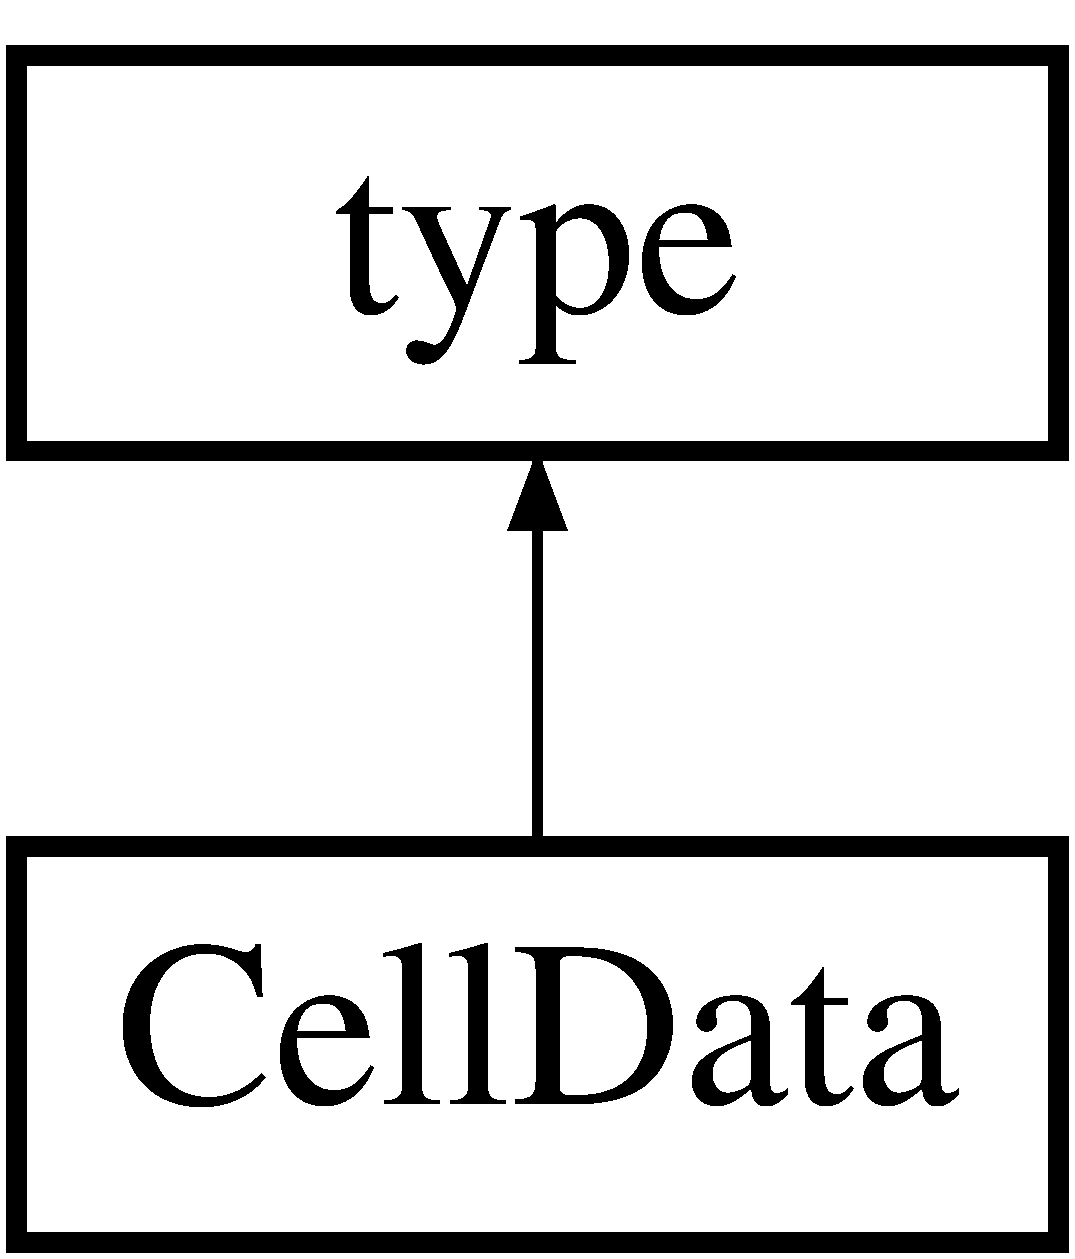
\includegraphics[height=2.000000cm]{classCellData}
\end{center}
\end{figure}
\subsection*{Public Types}
\begin{DoxyCompactItemize}
\item 
typedef \+::\hyperlink{classDataArray__t}{Data\+Array\+\_\+t} \hyperlink{classCellData_a3b277b87cd25225dc944f250bd52057d}{Data\+Array\+\_\+type}
\item 
typedef \+::xsd\+::cxx\+::tree\+::sequence$<$ \hyperlink{classCellData_a3b277b87cd25225dc944f250bd52057d}{Data\+Array\+\_\+type} $>$ \hyperlink{classCellData_a52b0c8e18ccdb06ed9e6ae76cd809c4a}{Data\+Array\+\_\+sequence}
\item 
typedef Data\+Array\+\_\+sequence\+::iterator \hyperlink{classCellData_abe0f5b0713690cc81703132bcdccd51f}{Data\+Array\+\_\+iterator}
\item 
typedef Data\+Array\+\_\+sequence\+::const\+\_\+iterator \hyperlink{classCellData_a8213ea10f002fac23b5555ca0b2b2a21}{Data\+Array\+\_\+const\+\_\+iterator}
\item 
typedef \+::xsd\+::cxx\+::tree\+::traits$<$ \hyperlink{classCellData_a3b277b87cd25225dc944f250bd52057d}{Data\+Array\+\_\+type}, char $>$ \hyperlink{classCellData_a03e76eec5af05a6ac5512e9cb80300bd}{Data\+Array\+\_\+traits}
\end{DoxyCompactItemize}
\subsection*{Public Member Functions}
\begin{DoxyCompactItemize}
\item 
const \hyperlink{classCellData_a52b0c8e18ccdb06ed9e6ae76cd809c4a}{Data\+Array\+\_\+sequence} \& \hyperlink{classCellData_af12d2f299905eca541a999dafba1e7e3}{Data\+Array} () const 
\item 
\hyperlink{classCellData_a52b0c8e18ccdb06ed9e6ae76cd809c4a}{Data\+Array\+\_\+sequence} \& \hyperlink{classCellData_ac40c7e291f83e3e9fabfddeef14131f5}{Data\+Array} ()
\item 
void \hyperlink{classCellData_a9ee9fc1ef295b3ad2c4dc3e9e70ac357}{Data\+Array} (const \hyperlink{classCellData_a52b0c8e18ccdb06ed9e6ae76cd809c4a}{Data\+Array\+\_\+sequence} \&s)
\item 
\hyperlink{classCellData_a0d89ba23195659a1fcdc714fa27697a5}{Cell\+Data} ()
\item 
\hyperlink{classCellData_ac98b30101e2448016bfa96b9fa6ee18a}{Cell\+Data} (const \+::xercesc\+::\+D\+O\+M\+Element \&e,\+::\hyperlink{namespacexml__schema_a0612287d030cb2732d31a45b258fdc87}{xml\+\_\+schema\+::flags} f=0,\+::\hyperlink{namespacexml__schema_ada9aa30dc722e93ee2ed7243085402a5}{xml\+\_\+schema\+::container} $\ast$c=0)
\item 
\hyperlink{classCellData_ae93656ff9893f518c8f1cfdc611c8045}{Cell\+Data} (const \hyperlink{classCellData}{Cell\+Data} \&x,\+::\hyperlink{namespacexml__schema_a0612287d030cb2732d31a45b258fdc87}{xml\+\_\+schema\+::flags} f=0,\+::\hyperlink{namespacexml__schema_ada9aa30dc722e93ee2ed7243085402a5}{xml\+\_\+schema\+::container} $\ast$c=0)
\item 
virtual \hyperlink{classCellData}{Cell\+Data} $\ast$ \hyperlink{classCellData_aa17c3a153b3a7692dca562878f3fe3ad}{\+\_\+clone} (\+::\hyperlink{namespacexml__schema_a0612287d030cb2732d31a45b258fdc87}{xml\+\_\+schema\+::flags} f=0,\+::\hyperlink{namespacexml__schema_ada9aa30dc722e93ee2ed7243085402a5}{xml\+\_\+schema\+::container} $\ast$c=0) const 
\item 
\hyperlink{classCellData}{Cell\+Data} \& \hyperlink{classCellData_a42d87874818d38a583d898832b54b7fa}{operator=} (const \hyperlink{classCellData}{Cell\+Data} \&x)
\item 
virtual \hyperlink{classCellData_aaf439852120aadb5a267799e2a7bf2a3}{$\sim$\+Cell\+Data} ()
\end{DoxyCompactItemize}
\subsection*{Protected Member Functions}
\begin{DoxyCompactItemize}
\item 
void \hyperlink{classCellData_a85b0468d603457e811156927cb35a3fa}{parse} (\+::xsd\+::cxx\+::xml\+::dom\+::parser$<$ char $>$ \&,\+::\hyperlink{namespacexml__schema_a0612287d030cb2732d31a45b258fdc87}{xml\+\_\+schema\+::flags})
\end{DoxyCompactItemize}
\subsection*{Protected Attributes}
\begin{DoxyCompactItemize}
\item 
\hyperlink{classCellData_a52b0c8e18ccdb06ed9e6ae76cd809c4a}{Data\+Array\+\_\+sequence} \hyperlink{classCellData_a6dc3acb849afce77fd961dbcabaa9252}{Data\+Array\+\_\+}
\end{DoxyCompactItemize}


\subsection{Member Typedef Documentation}
\index{Cell\+Data@{Cell\+Data}!Data\+Array\+\_\+const\+\_\+iterator@{Data\+Array\+\_\+const\+\_\+iterator}}
\index{Data\+Array\+\_\+const\+\_\+iterator@{Data\+Array\+\_\+const\+\_\+iterator}!Cell\+Data@{Cell\+Data}}
\subsubsection[{\texorpdfstring{Data\+Array\+\_\+const\+\_\+iterator}{DataArray_const_iterator}}]{\setlength{\rightskip}{0pt plus 5cm}typedef Data\+Array\+\_\+sequence\+::const\+\_\+iterator {\bf Cell\+Data\+::\+Data\+Array\+\_\+const\+\_\+iterator}}\hypertarget{classCellData_a8213ea10f002fac23b5555ca0b2b2a21}{}\label{classCellData_a8213ea10f002fac23b5555ca0b2b2a21}
\index{Cell\+Data@{Cell\+Data}!Data\+Array\+\_\+iterator@{Data\+Array\+\_\+iterator}}
\index{Data\+Array\+\_\+iterator@{Data\+Array\+\_\+iterator}!Cell\+Data@{Cell\+Data}}
\subsubsection[{\texorpdfstring{Data\+Array\+\_\+iterator}{DataArray_iterator}}]{\setlength{\rightskip}{0pt plus 5cm}typedef Data\+Array\+\_\+sequence\+::iterator {\bf Cell\+Data\+::\+Data\+Array\+\_\+iterator}}\hypertarget{classCellData_abe0f5b0713690cc81703132bcdccd51f}{}\label{classCellData_abe0f5b0713690cc81703132bcdccd51f}
\index{Cell\+Data@{Cell\+Data}!Data\+Array\+\_\+sequence@{Data\+Array\+\_\+sequence}}
\index{Data\+Array\+\_\+sequence@{Data\+Array\+\_\+sequence}!Cell\+Data@{Cell\+Data}}
\subsubsection[{\texorpdfstring{Data\+Array\+\_\+sequence}{DataArray_sequence}}]{\setlength{\rightskip}{0pt plus 5cm}typedef \+::xsd\+::cxx\+::tree\+::sequence$<$ {\bf Data\+Array\+\_\+type} $>$ {\bf Cell\+Data\+::\+Data\+Array\+\_\+sequence}}\hypertarget{classCellData_a52b0c8e18ccdb06ed9e6ae76cd809c4a}{}\label{classCellData_a52b0c8e18ccdb06ed9e6ae76cd809c4a}
\index{Cell\+Data@{Cell\+Data}!Data\+Array\+\_\+traits@{Data\+Array\+\_\+traits}}
\index{Data\+Array\+\_\+traits@{Data\+Array\+\_\+traits}!Cell\+Data@{Cell\+Data}}
\subsubsection[{\texorpdfstring{Data\+Array\+\_\+traits}{DataArray_traits}}]{\setlength{\rightskip}{0pt plus 5cm}typedef \+::xsd\+::cxx\+::tree\+::traits$<$ {\bf Data\+Array\+\_\+type}, char $>$ {\bf Cell\+Data\+::\+Data\+Array\+\_\+traits}}\hypertarget{classCellData_a03e76eec5af05a6ac5512e9cb80300bd}{}\label{classCellData_a03e76eec5af05a6ac5512e9cb80300bd}
\index{Cell\+Data@{Cell\+Data}!Data\+Array\+\_\+type@{Data\+Array\+\_\+type}}
\index{Data\+Array\+\_\+type@{Data\+Array\+\_\+type}!Cell\+Data@{Cell\+Data}}
\subsubsection[{\texorpdfstring{Data\+Array\+\_\+type}{DataArray_type}}]{\setlength{\rightskip}{0pt plus 5cm}typedef \+::{\bf Data\+Array\+\_\+t} {\bf Cell\+Data\+::\+Data\+Array\+\_\+type}}\hypertarget{classCellData_a3b277b87cd25225dc944f250bd52057d}{}\label{classCellData_a3b277b87cd25225dc944f250bd52057d}


\subsection{Constructor \& Destructor Documentation}
\index{Cell\+Data@{Cell\+Data}!Cell\+Data@{Cell\+Data}}
\index{Cell\+Data@{Cell\+Data}!Cell\+Data@{Cell\+Data}}
\subsubsection[{\texorpdfstring{Cell\+Data()}{CellData()}}]{\setlength{\rightskip}{0pt plus 5cm}Cell\+Data\+::\+Cell\+Data (
\begin{DoxyParamCaption}
{}
\end{DoxyParamCaption}
)}\hypertarget{classCellData_a0d89ba23195659a1fcdc714fa27697a5}{}\label{classCellData_a0d89ba23195659a1fcdc714fa27697a5}
\index{Cell\+Data@{Cell\+Data}!Cell\+Data@{Cell\+Data}}
\index{Cell\+Data@{Cell\+Data}!Cell\+Data@{Cell\+Data}}
\subsubsection[{\texorpdfstring{Cell\+Data(const \+::xercesc\+::\+D\+O\+M\+Element \&e,\+::xml\+\_\+schema\+::flags f=0,\+::xml\+\_\+schema\+::container $\ast$c=0)}{CellData(const ::xercesc::DOMElement &e,::xml_schema::flags f=0,::xml_schema::container *c=0)}}]{\setlength{\rightskip}{0pt plus 5cm}Cell\+Data\+::\+Cell\+Data (
\begin{DoxyParamCaption}
\item[{const \+::xercesc\+::\+D\+O\+M\+Element \&}]{e, }
\item[{\+::{\bf xml\+\_\+schema\+::flags}}]{f = {\ttfamily 0}, }
\item[{\+::{\bf xml\+\_\+schema\+::container} $\ast$}]{c = {\ttfamily 0}}
\end{DoxyParamCaption}
)}\hypertarget{classCellData_ac98b30101e2448016bfa96b9fa6ee18a}{}\label{classCellData_ac98b30101e2448016bfa96b9fa6ee18a}
\index{Cell\+Data@{Cell\+Data}!Cell\+Data@{Cell\+Data}}
\index{Cell\+Data@{Cell\+Data}!Cell\+Data@{Cell\+Data}}
\subsubsection[{\texorpdfstring{Cell\+Data(const Cell\+Data \&x,\+::xml\+\_\+schema\+::flags f=0,\+::xml\+\_\+schema\+::container $\ast$c=0)}{CellData(const CellData &x,::xml_schema::flags f=0,::xml_schema::container *c=0)}}]{\setlength{\rightskip}{0pt plus 5cm}Cell\+Data\+::\+Cell\+Data (
\begin{DoxyParamCaption}
\item[{const {\bf Cell\+Data} \&}]{x, }
\item[{\+::{\bf xml\+\_\+schema\+::flags}}]{f = {\ttfamily 0}, }
\item[{\+::{\bf xml\+\_\+schema\+::container} $\ast$}]{c = {\ttfamily 0}}
\end{DoxyParamCaption}
)}\hypertarget{classCellData_ae93656ff9893f518c8f1cfdc611c8045}{}\label{classCellData_ae93656ff9893f518c8f1cfdc611c8045}
\index{Cell\+Data@{Cell\+Data}!````~Cell\+Data@{$\sim$\+Cell\+Data}}
\index{````~Cell\+Data@{$\sim$\+Cell\+Data}!Cell\+Data@{Cell\+Data}}
\subsubsection[{\texorpdfstring{$\sim$\+Cell\+Data()}{~CellData()}}]{\setlength{\rightskip}{0pt plus 5cm}Cell\+Data\+::$\sim$\+Cell\+Data (
\begin{DoxyParamCaption}
{}
\end{DoxyParamCaption}
)\hspace{0.3cm}{\ttfamily [virtual]}}\hypertarget{classCellData_aaf439852120aadb5a267799e2a7bf2a3}{}\label{classCellData_aaf439852120aadb5a267799e2a7bf2a3}


\subsection{Member Function Documentation}
\index{Cell\+Data@{Cell\+Data}!\+\_\+clone@{\+\_\+clone}}
\index{\+\_\+clone@{\+\_\+clone}!Cell\+Data@{Cell\+Data}}
\subsubsection[{\texorpdfstring{\+\_\+clone(\+::xml\+\_\+schema\+::flags f=0,\+::xml\+\_\+schema\+::container $\ast$c=0) const }{_clone(::xml_schema::flags f=0,::xml_schema::container *c=0) const }}]{\setlength{\rightskip}{0pt plus 5cm}{\bf Cell\+Data} $\ast$ Cell\+Data\+::\+\_\+clone (
\begin{DoxyParamCaption}
\item[{\+::{\bf xml\+\_\+schema\+::flags}}]{f = {\ttfamily 0}, }
\item[{\+::{\bf xml\+\_\+schema\+::container} $\ast$}]{c = {\ttfamily 0}}
\end{DoxyParamCaption}
) const\hspace{0.3cm}{\ttfamily [virtual]}}\hypertarget{classCellData_aa17c3a153b3a7692dca562878f3fe3ad}{}\label{classCellData_aa17c3a153b3a7692dca562878f3fe3ad}
\index{Cell\+Data@{Cell\+Data}!Data\+Array@{Data\+Array}}
\index{Data\+Array@{Data\+Array}!Cell\+Data@{Cell\+Data}}
\subsubsection[{\texorpdfstring{Data\+Array() const }{DataArray() const }}]{\setlength{\rightskip}{0pt plus 5cm}const {\bf Cell\+Data\+::\+Data\+Array\+\_\+sequence} \& Cell\+Data\+::\+Data\+Array (
\begin{DoxyParamCaption}
{}
\end{DoxyParamCaption}
) const}\hypertarget{classCellData_af12d2f299905eca541a999dafba1e7e3}{}\label{classCellData_af12d2f299905eca541a999dafba1e7e3}
\index{Cell\+Data@{Cell\+Data}!Data\+Array@{Data\+Array}}
\index{Data\+Array@{Data\+Array}!Cell\+Data@{Cell\+Data}}
\subsubsection[{\texorpdfstring{Data\+Array()}{DataArray()}}]{\setlength{\rightskip}{0pt plus 5cm}{\bf Cell\+Data\+::\+Data\+Array\+\_\+sequence} \& Cell\+Data\+::\+Data\+Array (
\begin{DoxyParamCaption}
{}
\end{DoxyParamCaption}
)}\hypertarget{classCellData_ac40c7e291f83e3e9fabfddeef14131f5}{}\label{classCellData_ac40c7e291f83e3e9fabfddeef14131f5}
\index{Cell\+Data@{Cell\+Data}!Data\+Array@{Data\+Array}}
\index{Data\+Array@{Data\+Array}!Cell\+Data@{Cell\+Data}}
\subsubsection[{\texorpdfstring{Data\+Array(const Data\+Array\+\_\+sequence \&s)}{DataArray(const DataArray_sequence &s)}}]{\setlength{\rightskip}{0pt plus 5cm}void Cell\+Data\+::\+Data\+Array (
\begin{DoxyParamCaption}
\item[{const {\bf Data\+Array\+\_\+sequence} \&}]{s}
\end{DoxyParamCaption}
)}\hypertarget{classCellData_a9ee9fc1ef295b3ad2c4dc3e9e70ac357}{}\label{classCellData_a9ee9fc1ef295b3ad2c4dc3e9e70ac357}
\index{Cell\+Data@{Cell\+Data}!operator=@{operator=}}
\index{operator=@{operator=}!Cell\+Data@{Cell\+Data}}
\subsubsection[{\texorpdfstring{operator=(const Cell\+Data \&x)}{operator=(const CellData &x)}}]{\setlength{\rightskip}{0pt plus 5cm}{\bf Cell\+Data} \& Cell\+Data\+::operator= (
\begin{DoxyParamCaption}
\item[{const {\bf Cell\+Data} \&}]{x}
\end{DoxyParamCaption}
)}\hypertarget{classCellData_a42d87874818d38a583d898832b54b7fa}{}\label{classCellData_a42d87874818d38a583d898832b54b7fa}
\index{Cell\+Data@{Cell\+Data}!parse@{parse}}
\index{parse@{parse}!Cell\+Data@{Cell\+Data}}
\subsubsection[{\texorpdfstring{parse(\+::xsd\+::cxx\+::xml\+::dom\+::parser$<$ char $>$ \&,\+::xml\+\_\+schema\+::flags)}{parse(::xsd::cxx::xml::dom::parser< char > &,::xml_schema::flags)}}]{\setlength{\rightskip}{0pt plus 5cm}void Cell\+Data\+::parse (
\begin{DoxyParamCaption}
\item[{\+::xsd\+::cxx\+::xml\+::dom\+::parser$<$ char $>$ \&}]{p, }
\item[{\+::{\bf xml\+\_\+schema\+::flags}}]{f}
\end{DoxyParamCaption}
)\hspace{0.3cm}{\ttfamily [protected]}}\hypertarget{classCellData_a85b0468d603457e811156927cb35a3fa}{}\label{classCellData_a85b0468d603457e811156927cb35a3fa}


\subsection{Member Data Documentation}
\index{Cell\+Data@{Cell\+Data}!Data\+Array\+\_\+@{Data\+Array\+\_\+}}
\index{Data\+Array\+\_\+@{Data\+Array\+\_\+}!Cell\+Data@{Cell\+Data}}
\subsubsection[{\texorpdfstring{Data\+Array\+\_\+}{DataArray_}}]{\setlength{\rightskip}{0pt plus 5cm}{\bf Data\+Array\+\_\+sequence} Cell\+Data\+::\+Data\+Array\+\_\+\hspace{0.3cm}{\ttfamily [protected]}}\hypertarget{classCellData_a6dc3acb849afce77fd961dbcabaa9252}{}\label{classCellData_a6dc3acb849afce77fd961dbcabaa9252}


The documentation for this class was generated from the following files\+:\begin{DoxyCompactItemize}
\item 
src/output\+Writer/\hyperlink{vtk-unstructured_8h}{vtk-\/unstructured.\+h}\item 
src/output\+Writer/\hyperlink{vtk-unstructured_8cpp}{vtk-\/unstructured.\+cpp}\end{DoxyCompactItemize}

\hypertarget{classCells}{}\section{Cells Class Reference}
\label{classCells}\index{Cells@{Cells}}


{\ttfamily \#include $<$vtk-\/unstructured.\+h$>$}

Inheritance diagram for Cells\+:\begin{figure}[H]
\begin{center}
\leavevmode
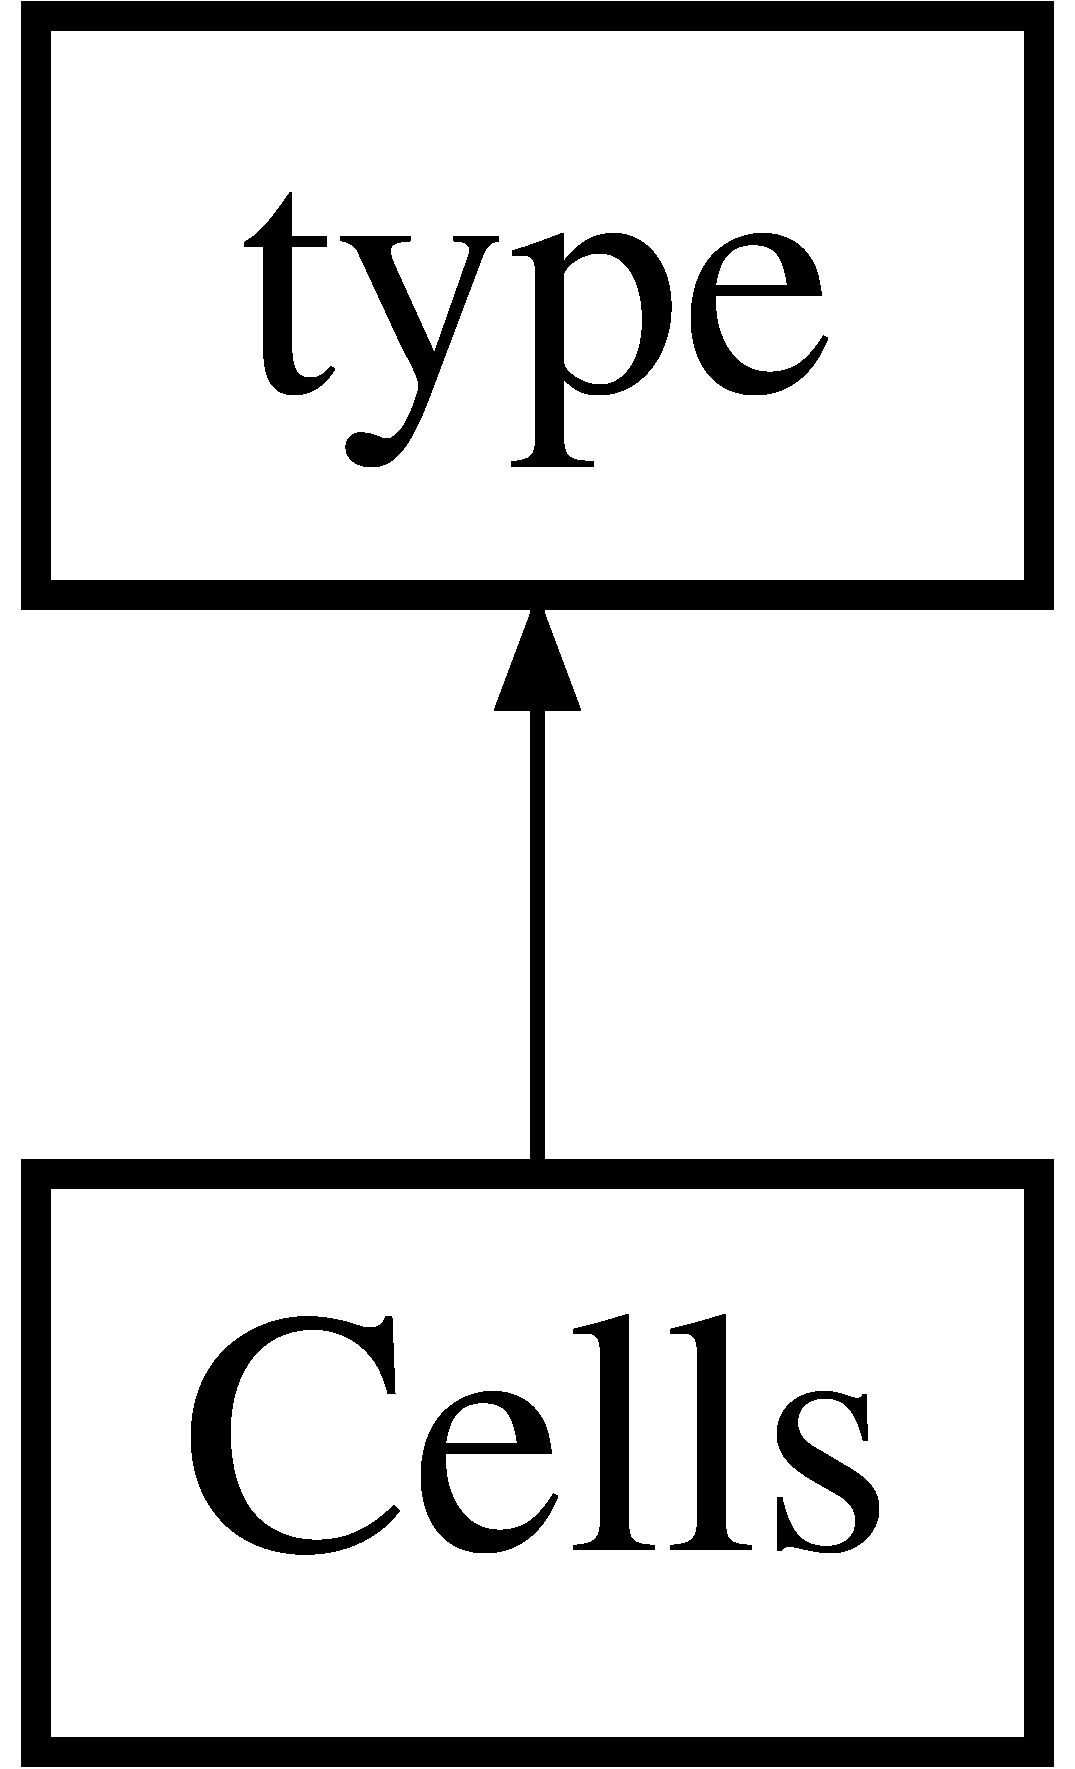
\includegraphics[height=2.000000cm]{classCells}
\end{center}
\end{figure}
\subsection*{Public Types}
\begin{DoxyCompactItemize}
\item 
typedef \+::\hyperlink{classDataArray__t}{Data\+Array\+\_\+t} \hyperlink{classCells_ad69e76337c22596e70b27d93c54dd722}{Data\+Array\+\_\+type}
\item 
typedef \+::xsd\+::cxx\+::tree\+::sequence$<$ \hyperlink{classCells_ad69e76337c22596e70b27d93c54dd722}{Data\+Array\+\_\+type} $>$ \hyperlink{classCells_ae2856ec1cc2c6d6a2ccac9de9a22c7b7}{Data\+Array\+\_\+sequence}
\item 
typedef Data\+Array\+\_\+sequence\+::iterator \hyperlink{classCells_a1873efdee2bb668676d01a7a5010faa2}{Data\+Array\+\_\+iterator}
\item 
typedef Data\+Array\+\_\+sequence\+::const\+\_\+iterator \hyperlink{classCells_ad01c81703074599471cd6159cdea1ac1}{Data\+Array\+\_\+const\+\_\+iterator}
\item 
typedef \+::xsd\+::cxx\+::tree\+::traits$<$ \hyperlink{classCells_ad69e76337c22596e70b27d93c54dd722}{Data\+Array\+\_\+type}, char $>$ \hyperlink{classCells_ac35ecebe10914f3d35e85589e998462b}{Data\+Array\+\_\+traits}
\end{DoxyCompactItemize}
\subsection*{Public Member Functions}
\begin{DoxyCompactItemize}
\item 
const \hyperlink{classCells_ae2856ec1cc2c6d6a2ccac9de9a22c7b7}{Data\+Array\+\_\+sequence} \& \hyperlink{classCells_a8844f4f5a352181f29e8589d72fba69f}{Data\+Array} () const 
\item 
\hyperlink{classCells_ae2856ec1cc2c6d6a2ccac9de9a22c7b7}{Data\+Array\+\_\+sequence} \& \hyperlink{classCells_a6114566d42273127f9cb92b1d0f09cb5}{Data\+Array} ()
\item 
void \hyperlink{classCells_a52c9971e15358118dd90ecf68b26601e}{Data\+Array} (const \hyperlink{classCells_ae2856ec1cc2c6d6a2ccac9de9a22c7b7}{Data\+Array\+\_\+sequence} \&s)
\item 
\hyperlink{classCells_a092d62bc15648a54755a413dbf9a2db0}{Cells} ()
\item 
\hyperlink{classCells_a79e3031094d928c8d275198201d44f0c}{Cells} (const \+::xercesc\+::\+D\+O\+M\+Element \&e,\+::\hyperlink{namespacexml__schema_a0612287d030cb2732d31a45b258fdc87}{xml\+\_\+schema\+::flags} f=0,\+::\hyperlink{namespacexml__schema_ada9aa30dc722e93ee2ed7243085402a5}{xml\+\_\+schema\+::container} $\ast$c=0)
\item 
\hyperlink{classCells_a9322653263fb302eb7068be10b1b364f}{Cells} (const \hyperlink{classCells}{Cells} \&x,\+::\hyperlink{namespacexml__schema_a0612287d030cb2732d31a45b258fdc87}{xml\+\_\+schema\+::flags} f=0,\+::\hyperlink{namespacexml__schema_ada9aa30dc722e93ee2ed7243085402a5}{xml\+\_\+schema\+::container} $\ast$c=0)
\item 
virtual \hyperlink{classCells}{Cells} $\ast$ \hyperlink{classCells_a67e7fa1cc404dcc4814011ca179f8a83}{\+\_\+clone} (\+::\hyperlink{namespacexml__schema_a0612287d030cb2732d31a45b258fdc87}{xml\+\_\+schema\+::flags} f=0,\+::\hyperlink{namespacexml__schema_ada9aa30dc722e93ee2ed7243085402a5}{xml\+\_\+schema\+::container} $\ast$c=0) const 
\item 
\hyperlink{classCells}{Cells} \& \hyperlink{classCells_a99df5dc58374d8a8d4794531e192f821}{operator=} (const \hyperlink{classCells}{Cells} \&x)
\item 
virtual \hyperlink{classCells_aab121634db81b439226a33fd099fb3c1}{$\sim$\+Cells} ()
\end{DoxyCompactItemize}
\subsection*{Protected Member Functions}
\begin{DoxyCompactItemize}
\item 
void \hyperlink{classCells_a90d91435b44503cd02934902007a3ace}{parse} (\+::xsd\+::cxx\+::xml\+::dom\+::parser$<$ char $>$ \&,\+::\hyperlink{namespacexml__schema_a0612287d030cb2732d31a45b258fdc87}{xml\+\_\+schema\+::flags})
\end{DoxyCompactItemize}
\subsection*{Protected Attributes}
\begin{DoxyCompactItemize}
\item 
\hyperlink{classCells_ae2856ec1cc2c6d6a2ccac9de9a22c7b7}{Data\+Array\+\_\+sequence} \hyperlink{classCells_aad066678c1454f4afa408bcf4f24c583}{Data\+Array\+\_\+}
\end{DoxyCompactItemize}


\subsection{Member Typedef Documentation}
\index{Cells@{Cells}!Data\+Array\+\_\+const\+\_\+iterator@{Data\+Array\+\_\+const\+\_\+iterator}}
\index{Data\+Array\+\_\+const\+\_\+iterator@{Data\+Array\+\_\+const\+\_\+iterator}!Cells@{Cells}}
\subsubsection[{\texorpdfstring{Data\+Array\+\_\+const\+\_\+iterator}{DataArray_const_iterator}}]{\setlength{\rightskip}{0pt plus 5cm}typedef Data\+Array\+\_\+sequence\+::const\+\_\+iterator {\bf Cells\+::\+Data\+Array\+\_\+const\+\_\+iterator}}\hypertarget{classCells_ad01c81703074599471cd6159cdea1ac1}{}\label{classCells_ad01c81703074599471cd6159cdea1ac1}
\index{Cells@{Cells}!Data\+Array\+\_\+iterator@{Data\+Array\+\_\+iterator}}
\index{Data\+Array\+\_\+iterator@{Data\+Array\+\_\+iterator}!Cells@{Cells}}
\subsubsection[{\texorpdfstring{Data\+Array\+\_\+iterator}{DataArray_iterator}}]{\setlength{\rightskip}{0pt plus 5cm}typedef Data\+Array\+\_\+sequence\+::iterator {\bf Cells\+::\+Data\+Array\+\_\+iterator}}\hypertarget{classCells_a1873efdee2bb668676d01a7a5010faa2}{}\label{classCells_a1873efdee2bb668676d01a7a5010faa2}
\index{Cells@{Cells}!Data\+Array\+\_\+sequence@{Data\+Array\+\_\+sequence}}
\index{Data\+Array\+\_\+sequence@{Data\+Array\+\_\+sequence}!Cells@{Cells}}
\subsubsection[{\texorpdfstring{Data\+Array\+\_\+sequence}{DataArray_sequence}}]{\setlength{\rightskip}{0pt plus 5cm}typedef \+::xsd\+::cxx\+::tree\+::sequence$<$ {\bf Data\+Array\+\_\+type} $>$ {\bf Cells\+::\+Data\+Array\+\_\+sequence}}\hypertarget{classCells_ae2856ec1cc2c6d6a2ccac9de9a22c7b7}{}\label{classCells_ae2856ec1cc2c6d6a2ccac9de9a22c7b7}
\index{Cells@{Cells}!Data\+Array\+\_\+traits@{Data\+Array\+\_\+traits}}
\index{Data\+Array\+\_\+traits@{Data\+Array\+\_\+traits}!Cells@{Cells}}
\subsubsection[{\texorpdfstring{Data\+Array\+\_\+traits}{DataArray_traits}}]{\setlength{\rightskip}{0pt plus 5cm}typedef \+::xsd\+::cxx\+::tree\+::traits$<$ {\bf Data\+Array\+\_\+type}, char $>$ {\bf Cells\+::\+Data\+Array\+\_\+traits}}\hypertarget{classCells_ac35ecebe10914f3d35e85589e998462b}{}\label{classCells_ac35ecebe10914f3d35e85589e998462b}
\index{Cells@{Cells}!Data\+Array\+\_\+type@{Data\+Array\+\_\+type}}
\index{Data\+Array\+\_\+type@{Data\+Array\+\_\+type}!Cells@{Cells}}
\subsubsection[{\texorpdfstring{Data\+Array\+\_\+type}{DataArray_type}}]{\setlength{\rightskip}{0pt plus 5cm}typedef \+::{\bf Data\+Array\+\_\+t} {\bf Cells\+::\+Data\+Array\+\_\+type}}\hypertarget{classCells_ad69e76337c22596e70b27d93c54dd722}{}\label{classCells_ad69e76337c22596e70b27d93c54dd722}


\subsection{Constructor \& Destructor Documentation}
\index{Cells@{Cells}!Cells@{Cells}}
\index{Cells@{Cells}!Cells@{Cells}}
\subsubsection[{\texorpdfstring{Cells()}{Cells()}}]{\setlength{\rightskip}{0pt plus 5cm}Cells\+::\+Cells (
\begin{DoxyParamCaption}
{}
\end{DoxyParamCaption}
)}\hypertarget{classCells_a092d62bc15648a54755a413dbf9a2db0}{}\label{classCells_a092d62bc15648a54755a413dbf9a2db0}
\index{Cells@{Cells}!Cells@{Cells}}
\index{Cells@{Cells}!Cells@{Cells}}
\subsubsection[{\texorpdfstring{Cells(const \+::xercesc\+::\+D\+O\+M\+Element \&e,\+::xml\+\_\+schema\+::flags f=0,\+::xml\+\_\+schema\+::container $\ast$c=0)}{Cells(const ::xercesc::DOMElement &e,::xml_schema::flags f=0,::xml_schema::container *c=0)}}]{\setlength{\rightskip}{0pt plus 5cm}Cells\+::\+Cells (
\begin{DoxyParamCaption}
\item[{const \+::xercesc\+::\+D\+O\+M\+Element \&}]{e, }
\item[{\+::{\bf xml\+\_\+schema\+::flags}}]{f = {\ttfamily 0}, }
\item[{\+::{\bf xml\+\_\+schema\+::container} $\ast$}]{c = {\ttfamily 0}}
\end{DoxyParamCaption}
)}\hypertarget{classCells_a79e3031094d928c8d275198201d44f0c}{}\label{classCells_a79e3031094d928c8d275198201d44f0c}
\index{Cells@{Cells}!Cells@{Cells}}
\index{Cells@{Cells}!Cells@{Cells}}
\subsubsection[{\texorpdfstring{Cells(const Cells \&x,\+::xml\+\_\+schema\+::flags f=0,\+::xml\+\_\+schema\+::container $\ast$c=0)}{Cells(const Cells &x,::xml_schema::flags f=0,::xml_schema::container *c=0)}}]{\setlength{\rightskip}{0pt plus 5cm}Cells\+::\+Cells (
\begin{DoxyParamCaption}
\item[{const {\bf Cells} \&}]{x, }
\item[{\+::{\bf xml\+\_\+schema\+::flags}}]{f = {\ttfamily 0}, }
\item[{\+::{\bf xml\+\_\+schema\+::container} $\ast$}]{c = {\ttfamily 0}}
\end{DoxyParamCaption}
)}\hypertarget{classCells_a9322653263fb302eb7068be10b1b364f}{}\label{classCells_a9322653263fb302eb7068be10b1b364f}
\index{Cells@{Cells}!````~Cells@{$\sim$\+Cells}}
\index{````~Cells@{$\sim$\+Cells}!Cells@{Cells}}
\subsubsection[{\texorpdfstring{$\sim$\+Cells()}{~Cells()}}]{\setlength{\rightskip}{0pt plus 5cm}Cells\+::$\sim$\+Cells (
\begin{DoxyParamCaption}
{}
\end{DoxyParamCaption}
)\hspace{0.3cm}{\ttfamily [virtual]}}\hypertarget{classCells_aab121634db81b439226a33fd099fb3c1}{}\label{classCells_aab121634db81b439226a33fd099fb3c1}


\subsection{Member Function Documentation}
\index{Cells@{Cells}!\+\_\+clone@{\+\_\+clone}}
\index{\+\_\+clone@{\+\_\+clone}!Cells@{Cells}}
\subsubsection[{\texorpdfstring{\+\_\+clone(\+::xml\+\_\+schema\+::flags f=0,\+::xml\+\_\+schema\+::container $\ast$c=0) const }{_clone(::xml_schema::flags f=0,::xml_schema::container *c=0) const }}]{\setlength{\rightskip}{0pt plus 5cm}{\bf Cells} $\ast$ Cells\+::\+\_\+clone (
\begin{DoxyParamCaption}
\item[{\+::{\bf xml\+\_\+schema\+::flags}}]{f = {\ttfamily 0}, }
\item[{\+::{\bf xml\+\_\+schema\+::container} $\ast$}]{c = {\ttfamily 0}}
\end{DoxyParamCaption}
) const\hspace{0.3cm}{\ttfamily [virtual]}}\hypertarget{classCells_a67e7fa1cc404dcc4814011ca179f8a83}{}\label{classCells_a67e7fa1cc404dcc4814011ca179f8a83}
\index{Cells@{Cells}!Data\+Array@{Data\+Array}}
\index{Data\+Array@{Data\+Array}!Cells@{Cells}}
\subsubsection[{\texorpdfstring{Data\+Array() const }{DataArray() const }}]{\setlength{\rightskip}{0pt plus 5cm}const {\bf Cells\+::\+Data\+Array\+\_\+sequence} \& Cells\+::\+Data\+Array (
\begin{DoxyParamCaption}
{}
\end{DoxyParamCaption}
) const}\hypertarget{classCells_a8844f4f5a352181f29e8589d72fba69f}{}\label{classCells_a8844f4f5a352181f29e8589d72fba69f}
\index{Cells@{Cells}!Data\+Array@{Data\+Array}}
\index{Data\+Array@{Data\+Array}!Cells@{Cells}}
\subsubsection[{\texorpdfstring{Data\+Array()}{DataArray()}}]{\setlength{\rightskip}{0pt plus 5cm}{\bf Cells\+::\+Data\+Array\+\_\+sequence} \& Cells\+::\+Data\+Array (
\begin{DoxyParamCaption}
{}
\end{DoxyParamCaption}
)}\hypertarget{classCells_a6114566d42273127f9cb92b1d0f09cb5}{}\label{classCells_a6114566d42273127f9cb92b1d0f09cb5}
\index{Cells@{Cells}!Data\+Array@{Data\+Array}}
\index{Data\+Array@{Data\+Array}!Cells@{Cells}}
\subsubsection[{\texorpdfstring{Data\+Array(const Data\+Array\+\_\+sequence \&s)}{DataArray(const DataArray_sequence &s)}}]{\setlength{\rightskip}{0pt plus 5cm}void Cells\+::\+Data\+Array (
\begin{DoxyParamCaption}
\item[{const {\bf Data\+Array\+\_\+sequence} \&}]{s}
\end{DoxyParamCaption}
)}\hypertarget{classCells_a52c9971e15358118dd90ecf68b26601e}{}\label{classCells_a52c9971e15358118dd90ecf68b26601e}
\index{Cells@{Cells}!operator=@{operator=}}
\index{operator=@{operator=}!Cells@{Cells}}
\subsubsection[{\texorpdfstring{operator=(const Cells \&x)}{operator=(const Cells &x)}}]{\setlength{\rightskip}{0pt plus 5cm}{\bf Cells} \& Cells\+::operator= (
\begin{DoxyParamCaption}
\item[{const {\bf Cells} \&}]{x}
\end{DoxyParamCaption}
)}\hypertarget{classCells_a99df5dc58374d8a8d4794531e192f821}{}\label{classCells_a99df5dc58374d8a8d4794531e192f821}
\index{Cells@{Cells}!parse@{parse}}
\index{parse@{parse}!Cells@{Cells}}
\subsubsection[{\texorpdfstring{parse(\+::xsd\+::cxx\+::xml\+::dom\+::parser$<$ char $>$ \&,\+::xml\+\_\+schema\+::flags)}{parse(::xsd::cxx::xml::dom::parser< char > &,::xml_schema::flags)}}]{\setlength{\rightskip}{0pt plus 5cm}void Cells\+::parse (
\begin{DoxyParamCaption}
\item[{\+::xsd\+::cxx\+::xml\+::dom\+::parser$<$ char $>$ \&}]{p, }
\item[{\+::{\bf xml\+\_\+schema\+::flags}}]{f}
\end{DoxyParamCaption}
)\hspace{0.3cm}{\ttfamily [protected]}}\hypertarget{classCells_a90d91435b44503cd02934902007a3ace}{}\label{classCells_a90d91435b44503cd02934902007a3ace}


\subsection{Member Data Documentation}
\index{Cells@{Cells}!Data\+Array\+\_\+@{Data\+Array\+\_\+}}
\index{Data\+Array\+\_\+@{Data\+Array\+\_\+}!Cells@{Cells}}
\subsubsection[{\texorpdfstring{Data\+Array\+\_\+}{DataArray_}}]{\setlength{\rightskip}{0pt plus 5cm}{\bf Data\+Array\+\_\+sequence} Cells\+::\+Data\+Array\+\_\+\hspace{0.3cm}{\ttfamily [protected]}}\hypertarget{classCells_aad066678c1454f4afa408bcf4f24c583}{}\label{classCells_aad066678c1454f4afa408bcf4f24c583}


The documentation for this class was generated from the following files\+:\begin{DoxyCompactItemize}
\item 
src/output\+Writer/\hyperlink{vtk-unstructured_8h}{vtk-\/unstructured.\+h}\item 
src/output\+Writer/\hyperlink{vtk-unstructured_8cpp}{vtk-\/unstructured.\+cpp}\end{DoxyCompactItemize}

\hypertarget{classoutputWriter_1_1CSVWriter}{}\section{output\+Writer\+:\+:C\+S\+V\+Writer Class Reference}
\label{classoutputWriter_1_1CSVWriter}\index{output\+Writer\+::\+C\+S\+V\+Writer@{output\+Writer\+::\+C\+S\+V\+Writer}}


{\ttfamily \#include $<$C\+S\+V\+Writer.\+h$>$}

\subsection*{Public Member Functions}
\begin{DoxyCompactItemize}
\item 
\hyperlink{classoutputWriter_1_1CSVWriter_ad69d499bac14025b61130bce1fad9bc1}{C\+S\+V\+Writer} (int \hyperlink{classoutputWriter_1_1CSVWriter_aff7fb0f68a0a6823118997606ed688a2}{bucket\+Num}, float \hyperlink{classoutputWriter_1_1CSVWriter_ab72029e6c3e7fe219e71f41fe876501c}{sizeX})
\item 
virtual \hyperlink{classoutputWriter_1_1CSVWriter_acc822830c8c0672ccaec0e8eb664e423}{$\sim$\+C\+S\+V\+Writer} ()
\item 
void \hyperlink{classoutputWriter_1_1CSVWriter_a5bb4fca2ba4d90ac2466257e6d5ea359}{plot\+Particles} (std\+::list$<$ \hyperlink{classParticle}{Particle} $>$ particles, const std\+::string \&filename, int iteration)
\end{DoxyCompactItemize}
\subsection*{Private Attributes}
\begin{DoxyCompactItemize}
\item 
int \hyperlink{classoutputWriter_1_1CSVWriter_aff7fb0f68a0a6823118997606ed688a2}{bucket\+Num}
\item 
float \hyperlink{classoutputWriter_1_1CSVWriter_ab72029e6c3e7fe219e71f41fe876501c}{sizeX}
\end{DoxyCompactItemize}


\subsection{Constructor \& Destructor Documentation}
\index{output\+Writer\+::\+C\+S\+V\+Writer@{output\+Writer\+::\+C\+S\+V\+Writer}!C\+S\+V\+Writer@{C\+S\+V\+Writer}}
\index{C\+S\+V\+Writer@{C\+S\+V\+Writer}!output\+Writer\+::\+C\+S\+V\+Writer@{output\+Writer\+::\+C\+S\+V\+Writer}}
\subsubsection[{\texorpdfstring{C\+S\+V\+Writer(int bucket\+Num, float size\+X)}{CSVWriter(int bucketNum, float sizeX)}}]{\setlength{\rightskip}{0pt plus 5cm}output\+Writer\+::\+C\+S\+V\+Writer\+::\+C\+S\+V\+Writer (
\begin{DoxyParamCaption}
\item[{int}]{bucket\+Num, }
\item[{float}]{sizeX}
\end{DoxyParamCaption}
)}\hypertarget{classoutputWriter_1_1CSVWriter_ad69d499bac14025b61130bce1fad9bc1}{}\label{classoutputWriter_1_1CSVWriter_ad69d499bac14025b61130bce1fad9bc1}
\index{output\+Writer\+::\+C\+S\+V\+Writer@{output\+Writer\+::\+C\+S\+V\+Writer}!````~C\+S\+V\+Writer@{$\sim$\+C\+S\+V\+Writer}}
\index{````~C\+S\+V\+Writer@{$\sim$\+C\+S\+V\+Writer}!output\+Writer\+::\+C\+S\+V\+Writer@{output\+Writer\+::\+C\+S\+V\+Writer}}
\subsubsection[{\texorpdfstring{$\sim$\+C\+S\+V\+Writer()}{~CSVWriter()}}]{\setlength{\rightskip}{0pt plus 5cm}output\+Writer\+::\+C\+S\+V\+Writer\+::$\sim$\+C\+S\+V\+Writer (
\begin{DoxyParamCaption}
{}
\end{DoxyParamCaption}
)\hspace{0.3cm}{\ttfamily [virtual]}}\hypertarget{classoutputWriter_1_1CSVWriter_acc822830c8c0672ccaec0e8eb664e423}{}\label{classoutputWriter_1_1CSVWriter_acc822830c8c0672ccaec0e8eb664e423}


\subsection{Member Function Documentation}
\index{output\+Writer\+::\+C\+S\+V\+Writer@{output\+Writer\+::\+C\+S\+V\+Writer}!plot\+Particles@{plot\+Particles}}
\index{plot\+Particles@{plot\+Particles}!output\+Writer\+::\+C\+S\+V\+Writer@{output\+Writer\+::\+C\+S\+V\+Writer}}
\subsubsection[{\texorpdfstring{plot\+Particles(std\+::list$<$ Particle $>$ particles, const std\+::string \&filename, int iteration)}{plotParticles(std::list< Particle > particles, const std::string &filename, int iteration)}}]{\setlength{\rightskip}{0pt plus 5cm}void output\+Writer\+::\+C\+S\+V\+Writer\+::plot\+Particles (
\begin{DoxyParamCaption}
\item[{std\+::list$<$ {\bf Particle} $>$}]{particles, }
\item[{const std\+::string \&}]{filename, }
\item[{int}]{iteration}
\end{DoxyParamCaption}
)}\hypertarget{classoutputWriter_1_1CSVWriter_a5bb4fca2ba4d90ac2466257e6d5ea359}{}\label{classoutputWriter_1_1CSVWriter_a5bb4fca2ba4d90ac2466257e6d5ea359}


\subsection{Member Data Documentation}
\index{output\+Writer\+::\+C\+S\+V\+Writer@{output\+Writer\+::\+C\+S\+V\+Writer}!bucket\+Num@{bucket\+Num}}
\index{bucket\+Num@{bucket\+Num}!output\+Writer\+::\+C\+S\+V\+Writer@{output\+Writer\+::\+C\+S\+V\+Writer}}
\subsubsection[{\texorpdfstring{bucket\+Num}{bucketNum}}]{\setlength{\rightskip}{0pt plus 5cm}int output\+Writer\+::\+C\+S\+V\+Writer\+::bucket\+Num\hspace{0.3cm}{\ttfamily [private]}}\hypertarget{classoutputWriter_1_1CSVWriter_aff7fb0f68a0a6823118997606ed688a2}{}\label{classoutputWriter_1_1CSVWriter_aff7fb0f68a0a6823118997606ed688a2}
\index{output\+Writer\+::\+C\+S\+V\+Writer@{output\+Writer\+::\+C\+S\+V\+Writer}!sizeX@{sizeX}}
\index{sizeX@{sizeX}!output\+Writer\+::\+C\+S\+V\+Writer@{output\+Writer\+::\+C\+S\+V\+Writer}}
\subsubsection[{\texorpdfstring{sizeX}{sizeX}}]{\setlength{\rightskip}{0pt plus 5cm}float output\+Writer\+::\+C\+S\+V\+Writer\+::sizeX\hspace{0.3cm}{\ttfamily [private]}}\hypertarget{classoutputWriter_1_1CSVWriter_ab72029e6c3e7fe219e71f41fe876501c}{}\label{classoutputWriter_1_1CSVWriter_ab72029e6c3e7fe219e71f41fe876501c}


The documentation for this class was generated from the following files\+:\begin{DoxyCompactItemize}
\item 
src/output\+Writer/\hyperlink{CSVWriter_8h}{C\+S\+V\+Writer.\+h}\item 
src/output\+Writer/\hyperlink{CSVWriter_8cpp}{C\+S\+V\+Writer.\+cpp}\end{DoxyCompactItemize}

\hypertarget{classcuboid__t}{}\section{cuboid\+\_\+t Class Reference}
\label{classcuboid__t}\index{cuboid\+\_\+t@{cuboid\+\_\+t}}


{\ttfamily \#include $<$particle\+\_\+input.\+h$>$}

Inheritance diagram for cuboid\+\_\+t\+:\begin{figure}[H]
\begin{center}
\leavevmode
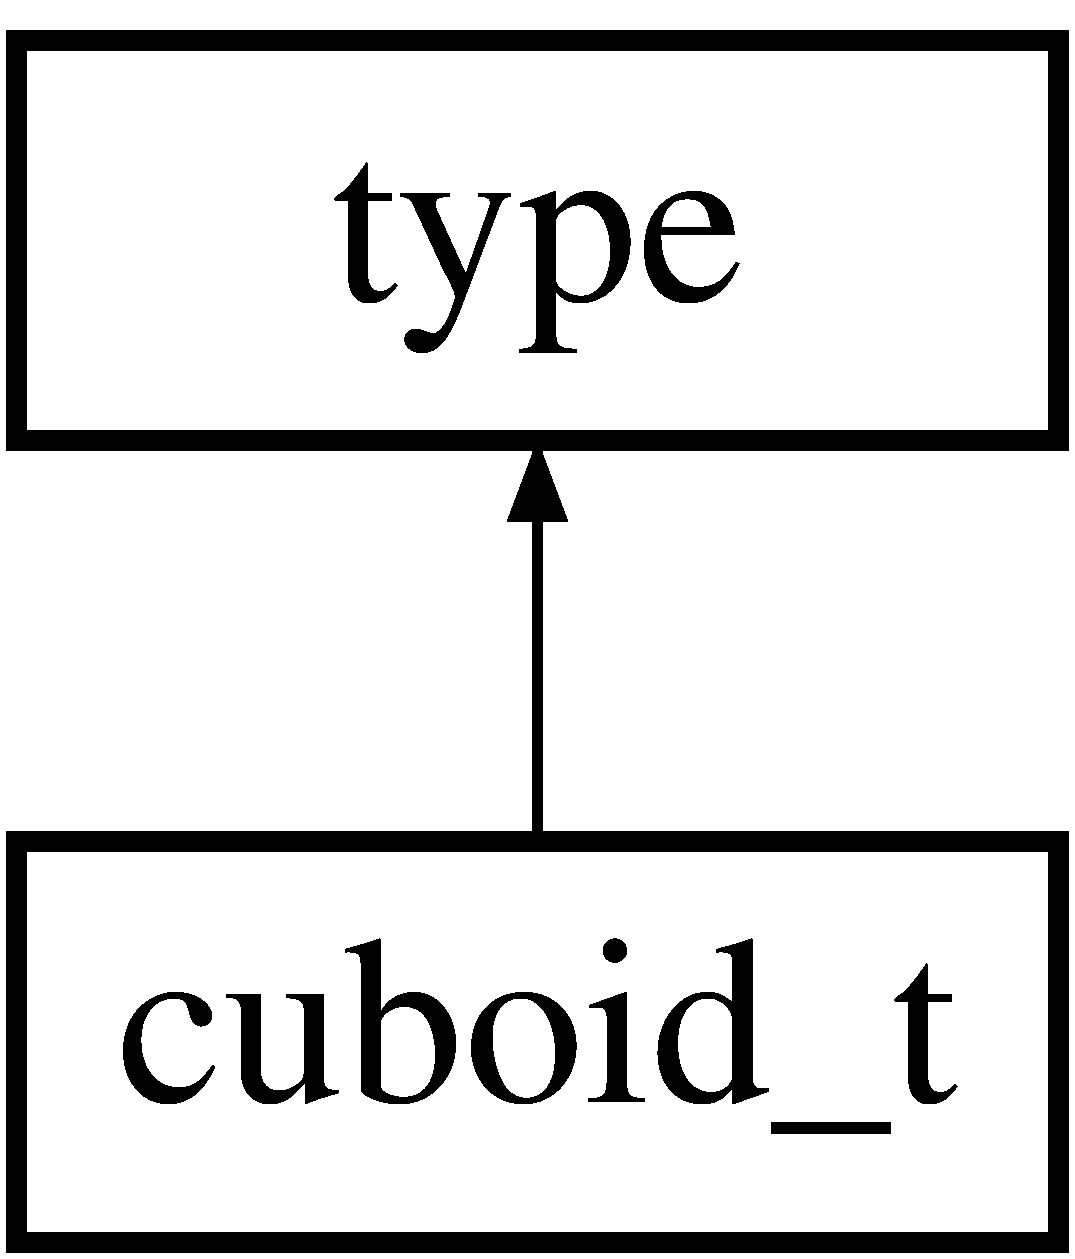
\includegraphics[height=2.000000cm]{classcuboid__t}
\end{center}
\end{figure}
\subsection*{Public Types}
\begin{DoxyCompactItemize}
\item 
typedef \+::\hyperlink{classvector__t}{vector\+\_\+t} \hyperlink{classcuboid__t_aa3c19ea94c59ed982641ca39a420a041}{coord\+\_\+type}
\item 
typedef \+::xsd\+::cxx\+::tree\+::traits$<$ \hyperlink{classcuboid__t_aa3c19ea94c59ed982641ca39a420a041}{coord\+\_\+type}, char $>$ \hyperlink{classcuboid__t_a9aa6a75493e47a7f976c08e9be597b54}{coord\+\_\+traits}
\item 
typedef \+::\hyperlink{classint__vector__t}{int\+\_\+vector\+\_\+t} \hyperlink{classcuboid__t_a0992ec1724eb71e76babf752bbe9189b}{dimension\+\_\+type}
\item 
typedef \+::xsd\+::cxx\+::tree\+::traits$<$ \hyperlink{classcuboid__t_a0992ec1724eb71e76babf752bbe9189b}{dimension\+\_\+type}, char $>$ \hyperlink{classcuboid__t_aed028730d651f8447c9243431c31b176}{dimension\+\_\+traits}
\item 
typedef \+::\hyperlink{namespacexml__schema_ad7e04ab17bba0b3fdde43fb79ef6ed87}{xml\+\_\+schema\+::float\+\_\+} \hyperlink{classcuboid__t_a48025da79e9243b8b1e34e696c22e06d}{mesh\+\_\+type}
\item 
typedef \+::xsd\+::cxx\+::tree\+::traits$<$ \hyperlink{classcuboid__t_a48025da79e9243b8b1e34e696c22e06d}{mesh\+\_\+type}, char $>$ \hyperlink{classcuboid__t_a67db60662cfd845bfe24613ab89f75bb}{mesh\+\_\+traits}
\item 
typedef \+::\hyperlink{classvector__t}{vector\+\_\+t} \hyperlink{classcuboid__t_a71c58ac42113feacf576245bc43d8dde}{velocity\+\_\+type}
\item 
typedef \+::xsd\+::cxx\+::tree\+::traits$<$ \hyperlink{classcuboid__t_a71c58ac42113feacf576245bc43d8dde}{velocity\+\_\+type}, char $>$ \hyperlink{classcuboid__t_ae9e44d76c104412fa2f0fb02e0b8b6f2}{velocity\+\_\+traits}
\item 
typedef \+::\hyperlink{namespacexml__schema_acfa24ac68e1a188e7f44c36f7a158bf4}{xml\+\_\+schema\+::int\+\_\+} \hyperlink{classcuboid__t_a6fb75392e8d31d56062e18b6aa2adc8a}{type\+\_\+type}
\item 
typedef \+::xsd\+::cxx\+::tree\+::traits$<$ \hyperlink{classcuboid__t_a6fb75392e8d31d56062e18b6aa2adc8a}{type\+\_\+type}, char $>$ \hyperlink{classcuboid__t_af1801e353fa239baa79a76f6942f40f9}{type\+\_\+traits}
\end{DoxyCompactItemize}
\subsection*{Public Member Functions}
\begin{DoxyCompactItemize}
\item 
const \hyperlink{classcuboid__t_aa3c19ea94c59ed982641ca39a420a041}{coord\+\_\+type} \& \hyperlink{classcuboid__t_aa59d1259b69308fc019bd515501ce9c5}{coord} () const 
\item 
\hyperlink{classcuboid__t_aa3c19ea94c59ed982641ca39a420a041}{coord\+\_\+type} \& \hyperlink{classcuboid__t_a08bd56077bd7a5fa0b3a675db1ffb599}{coord} ()
\item 
void \hyperlink{classcuboid__t_afc00b4b51e918a973044a6dbf149e83b}{coord} (const \hyperlink{classcuboid__t_aa3c19ea94c59ed982641ca39a420a041}{coord\+\_\+type} \&x)
\item 
void \hyperlink{classcuboid__t_a5b52cff02eedff7b6e09753cde98add2}{coord} (\+::std\+::unique\+\_\+ptr$<$ \hyperlink{classcuboid__t_aa3c19ea94c59ed982641ca39a420a041}{coord\+\_\+type} $>$ p)
\item 
const \hyperlink{classcuboid__t_a0992ec1724eb71e76babf752bbe9189b}{dimension\+\_\+type} \& \hyperlink{classcuboid__t_a26f2220ad94483e4b94a930cf1983d9f}{dimension} () const 
\item 
\hyperlink{classcuboid__t_a0992ec1724eb71e76babf752bbe9189b}{dimension\+\_\+type} \& \hyperlink{classcuboid__t_aea33ff632180a4a3e6d6610f51d0877b}{dimension} ()
\item 
void \hyperlink{classcuboid__t_a3410f77c6419273a2b2205af00778432}{dimension} (const \hyperlink{classcuboid__t_a0992ec1724eb71e76babf752bbe9189b}{dimension\+\_\+type} \&x)
\item 
void \hyperlink{classcuboid__t_aa193e0ba063d2df2555a0c5ddaf775c2}{dimension} (\+::std\+::unique\+\_\+ptr$<$ \hyperlink{classcuboid__t_a0992ec1724eb71e76babf752bbe9189b}{dimension\+\_\+type} $>$ p)
\item 
const \hyperlink{classcuboid__t_a48025da79e9243b8b1e34e696c22e06d}{mesh\+\_\+type} \& \hyperlink{classcuboid__t_ab342d2b7cefd9e06ba5071c8154e2d06}{mesh} () const 
\item 
\hyperlink{classcuboid__t_a48025da79e9243b8b1e34e696c22e06d}{mesh\+\_\+type} \& \hyperlink{classcuboid__t_a25e6df90635b65b85ecbf068ba917885}{mesh} ()
\item 
void \hyperlink{classcuboid__t_acafe29403b610ef652d69291bc1640c5}{mesh} (const \hyperlink{classcuboid__t_a48025da79e9243b8b1e34e696c22e06d}{mesh\+\_\+type} \&x)
\item 
const \hyperlink{classcuboid__t_a71c58ac42113feacf576245bc43d8dde}{velocity\+\_\+type} \& \hyperlink{classcuboid__t_a0a63a4f09fcc1006371cd5074aa5daa1}{velocity} () const 
\item 
\hyperlink{classcuboid__t_a71c58ac42113feacf576245bc43d8dde}{velocity\+\_\+type} \& \hyperlink{classcuboid__t_ac6f84c9ffb3b3bd15ef46dfe9f7488aa}{velocity} ()
\item 
void \hyperlink{classcuboid__t_a5792df33b443ebb4567d6065e7220e55}{velocity} (const \hyperlink{classcuboid__t_a71c58ac42113feacf576245bc43d8dde}{velocity\+\_\+type} \&x)
\item 
void \hyperlink{classcuboid__t_aa94c0a4c68e70db1bd5e966b2ceb4795}{velocity} (\+::std\+::unique\+\_\+ptr$<$ \hyperlink{classcuboid__t_a71c58ac42113feacf576245bc43d8dde}{velocity\+\_\+type} $>$ p)
\item 
const \hyperlink{classcuboid__t_a6fb75392e8d31d56062e18b6aa2adc8a}{type\+\_\+type} \& \hyperlink{classcuboid__t_a55195bf6362bb4a82c568d6561a4a00d}{type} () const 
\item 
\hyperlink{classcuboid__t_a6fb75392e8d31d56062e18b6aa2adc8a}{type\+\_\+type} \& \hyperlink{classcuboid__t_a1e4471fb01f14bb97ef46d94f4cc22e9}{type} ()
\item 
void \hyperlink{classcuboid__t_ae312cc3a069b53e3c09c5bdca5279ef1}{type} (const \hyperlink{classcuboid__t_a6fb75392e8d31d56062e18b6aa2adc8a}{type\+\_\+type} \&x)
\item 
\hyperlink{classcuboid__t_a806788c361e57c13e1d5f59637ebcdce}{cuboid\+\_\+t} (const \hyperlink{classcuboid__t_aa3c19ea94c59ed982641ca39a420a041}{coord\+\_\+type} \&, const \hyperlink{classcuboid__t_a0992ec1724eb71e76babf752bbe9189b}{dimension\+\_\+type} \&, const \hyperlink{classcuboid__t_a48025da79e9243b8b1e34e696c22e06d}{mesh\+\_\+type} \&, const \hyperlink{classcuboid__t_a71c58ac42113feacf576245bc43d8dde}{velocity\+\_\+type} \&, const \hyperlink{classcuboid__t_a6fb75392e8d31d56062e18b6aa2adc8a}{type\+\_\+type} \&)
\item 
\hyperlink{classcuboid__t_a22c19e96f12141bafd1b6ad465a1f1f3}{cuboid\+\_\+t} (\+::std\+::unique\+\_\+ptr$<$ \hyperlink{classcuboid__t_aa3c19ea94c59ed982641ca39a420a041}{coord\+\_\+type} $>$,\+::std\+::unique\+\_\+ptr$<$ \hyperlink{classcuboid__t_a0992ec1724eb71e76babf752bbe9189b}{dimension\+\_\+type} $>$, const \hyperlink{classcuboid__t_a48025da79e9243b8b1e34e696c22e06d}{mesh\+\_\+type} \&,\+::std\+::unique\+\_\+ptr$<$ \hyperlink{classcuboid__t_a71c58ac42113feacf576245bc43d8dde}{velocity\+\_\+type} $>$, const \hyperlink{classcuboid__t_a6fb75392e8d31d56062e18b6aa2adc8a}{type\+\_\+type} \&)
\item 
\hyperlink{classcuboid__t_afa1b7588ca19d8c5d00fb8c5dcf92bc8}{cuboid\+\_\+t} (const \+::xercesc\+::\+D\+O\+M\+Element \&e,\+::\hyperlink{namespacexml__schema_a0612287d030cb2732d31a45b258fdc87}{xml\+\_\+schema\+::flags} f=0,\+::\hyperlink{namespacexml__schema_ada9aa30dc722e93ee2ed7243085402a5}{xml\+\_\+schema\+::container} $\ast$c=0)
\item 
\hyperlink{classcuboid__t_a1574d539277176b5fff09a374c142c90}{cuboid\+\_\+t} (const \hyperlink{classcuboid__t}{cuboid\+\_\+t} \&x,\+::\hyperlink{namespacexml__schema_a0612287d030cb2732d31a45b258fdc87}{xml\+\_\+schema\+::flags} f=0,\+::\hyperlink{namespacexml__schema_ada9aa30dc722e93ee2ed7243085402a5}{xml\+\_\+schema\+::container} $\ast$c=0)
\item 
virtual \hyperlink{classcuboid__t}{cuboid\+\_\+t} $\ast$ \hyperlink{classcuboid__t_aa31bc17c300c78f7c15b08d60bbdefbf}{\+\_\+clone} (\+::\hyperlink{namespacexml__schema_a0612287d030cb2732d31a45b258fdc87}{xml\+\_\+schema\+::flags} f=0,\+::\hyperlink{namespacexml__schema_ada9aa30dc722e93ee2ed7243085402a5}{xml\+\_\+schema\+::container} $\ast$c=0) const 
\item 
\hyperlink{classcuboid__t}{cuboid\+\_\+t} \& \hyperlink{classcuboid__t_a63f90f88f500fa731186f53d2c668552}{operator=} (const \hyperlink{classcuboid__t}{cuboid\+\_\+t} \&x)
\item 
virtual \hyperlink{classcuboid__t_ad45791533f3643e2e2f565801c0ca20a}{$\sim$cuboid\+\_\+t} ()
\end{DoxyCompactItemize}
\subsection*{Protected Member Functions}
\begin{DoxyCompactItemize}
\item 
void \hyperlink{classcuboid__t_ab79e4219bf9a205aff7cbbda1207d138}{parse} (\+::xsd\+::cxx\+::xml\+::dom\+::parser$<$ char $>$ \&,\+::\hyperlink{namespacexml__schema_a0612287d030cb2732d31a45b258fdc87}{xml\+\_\+schema\+::flags})
\end{DoxyCompactItemize}
\subsection*{Protected Attributes}
\begin{DoxyCompactItemize}
\item 
\+::xsd\+::cxx\+::tree\+::one$<$ \hyperlink{classcuboid__t_aa3c19ea94c59ed982641ca39a420a041}{coord\+\_\+type} $>$ \hyperlink{classcuboid__t_ac230bff6b6def0f5d6aabaacc3538d38}{coord\+\_\+}
\item 
\+::xsd\+::cxx\+::tree\+::one$<$ \hyperlink{classcuboid__t_a0992ec1724eb71e76babf752bbe9189b}{dimension\+\_\+type} $>$ \hyperlink{classcuboid__t_a12a329c151427b69ab165a23ce32ed26}{dimension\+\_\+}
\item 
\+::xsd\+::cxx\+::tree\+::one$<$ \hyperlink{classcuboid__t_a48025da79e9243b8b1e34e696c22e06d}{mesh\+\_\+type} $>$ \hyperlink{classcuboid__t_aaac49c075536283060216167d0e71e80}{mesh\+\_\+}
\item 
\+::xsd\+::cxx\+::tree\+::one$<$ \hyperlink{classcuboid__t_a71c58ac42113feacf576245bc43d8dde}{velocity\+\_\+type} $>$ \hyperlink{classcuboid__t_a38590de341c9a52a3cced988ea26d891}{velocity\+\_\+}
\item 
\+::xsd\+::cxx\+::tree\+::one$<$ \hyperlink{classcuboid__t_a6fb75392e8d31d56062e18b6aa2adc8a}{type\+\_\+type} $>$ \hyperlink{classcuboid__t_a950799bbd14b31cd020481cba9092eb8}{type\+\_\+}
\end{DoxyCompactItemize}


\subsection{Member Typedef Documentation}
\index{cuboid\+\_\+t@{cuboid\+\_\+t}!coord\+\_\+traits@{coord\+\_\+traits}}
\index{coord\+\_\+traits@{coord\+\_\+traits}!cuboid\+\_\+t@{cuboid\+\_\+t}}
\subsubsection[{\texorpdfstring{coord\+\_\+traits}{coord_traits}}]{\setlength{\rightskip}{0pt plus 5cm}typedef \+::xsd\+::cxx\+::tree\+::traits$<$ {\bf coord\+\_\+type}, char $>$ {\bf cuboid\+\_\+t\+::coord\+\_\+traits}}\hypertarget{classcuboid__t_a9aa6a75493e47a7f976c08e9be597b54}{}\label{classcuboid__t_a9aa6a75493e47a7f976c08e9be597b54}
\index{cuboid\+\_\+t@{cuboid\+\_\+t}!coord\+\_\+type@{coord\+\_\+type}}
\index{coord\+\_\+type@{coord\+\_\+type}!cuboid\+\_\+t@{cuboid\+\_\+t}}
\subsubsection[{\texorpdfstring{coord\+\_\+type}{coord_type}}]{\setlength{\rightskip}{0pt plus 5cm}typedef \+::{\bf vector\+\_\+t} {\bf cuboid\+\_\+t\+::coord\+\_\+type}}\hypertarget{classcuboid__t_aa3c19ea94c59ed982641ca39a420a041}{}\label{classcuboid__t_aa3c19ea94c59ed982641ca39a420a041}
\index{cuboid\+\_\+t@{cuboid\+\_\+t}!dimension\+\_\+traits@{dimension\+\_\+traits}}
\index{dimension\+\_\+traits@{dimension\+\_\+traits}!cuboid\+\_\+t@{cuboid\+\_\+t}}
\subsubsection[{\texorpdfstring{dimension\+\_\+traits}{dimension_traits}}]{\setlength{\rightskip}{0pt plus 5cm}typedef \+::xsd\+::cxx\+::tree\+::traits$<$ {\bf dimension\+\_\+type}, char $>$ {\bf cuboid\+\_\+t\+::dimension\+\_\+traits}}\hypertarget{classcuboid__t_aed028730d651f8447c9243431c31b176}{}\label{classcuboid__t_aed028730d651f8447c9243431c31b176}
\index{cuboid\+\_\+t@{cuboid\+\_\+t}!dimension\+\_\+type@{dimension\+\_\+type}}
\index{dimension\+\_\+type@{dimension\+\_\+type}!cuboid\+\_\+t@{cuboid\+\_\+t}}
\subsubsection[{\texorpdfstring{dimension\+\_\+type}{dimension_type}}]{\setlength{\rightskip}{0pt plus 5cm}typedef \+::{\bf int\+\_\+vector\+\_\+t} {\bf cuboid\+\_\+t\+::dimension\+\_\+type}}\hypertarget{classcuboid__t_a0992ec1724eb71e76babf752bbe9189b}{}\label{classcuboid__t_a0992ec1724eb71e76babf752bbe9189b}
\index{cuboid\+\_\+t@{cuboid\+\_\+t}!mesh\+\_\+traits@{mesh\+\_\+traits}}
\index{mesh\+\_\+traits@{mesh\+\_\+traits}!cuboid\+\_\+t@{cuboid\+\_\+t}}
\subsubsection[{\texorpdfstring{mesh\+\_\+traits}{mesh_traits}}]{\setlength{\rightskip}{0pt plus 5cm}typedef \+::xsd\+::cxx\+::tree\+::traits$<$ {\bf mesh\+\_\+type}, char $>$ {\bf cuboid\+\_\+t\+::mesh\+\_\+traits}}\hypertarget{classcuboid__t_a67db60662cfd845bfe24613ab89f75bb}{}\label{classcuboid__t_a67db60662cfd845bfe24613ab89f75bb}
\index{cuboid\+\_\+t@{cuboid\+\_\+t}!mesh\+\_\+type@{mesh\+\_\+type}}
\index{mesh\+\_\+type@{mesh\+\_\+type}!cuboid\+\_\+t@{cuboid\+\_\+t}}
\subsubsection[{\texorpdfstring{mesh\+\_\+type}{mesh_type}}]{\setlength{\rightskip}{0pt plus 5cm}typedef \+::{\bf xml\+\_\+schema\+::float\+\_\+} {\bf cuboid\+\_\+t\+::mesh\+\_\+type}}\hypertarget{classcuboid__t_a48025da79e9243b8b1e34e696c22e06d}{}\label{classcuboid__t_a48025da79e9243b8b1e34e696c22e06d}
\index{cuboid\+\_\+t@{cuboid\+\_\+t}!type\+\_\+traits@{type\+\_\+traits}}
\index{type\+\_\+traits@{type\+\_\+traits}!cuboid\+\_\+t@{cuboid\+\_\+t}}
\subsubsection[{\texorpdfstring{type\+\_\+traits}{type_traits}}]{\setlength{\rightskip}{0pt plus 5cm}typedef \+::xsd\+::cxx\+::tree\+::traits$<$ {\bf type\+\_\+type}, char $>$ {\bf cuboid\+\_\+t\+::type\+\_\+traits}}\hypertarget{classcuboid__t_af1801e353fa239baa79a76f6942f40f9}{}\label{classcuboid__t_af1801e353fa239baa79a76f6942f40f9}
\index{cuboid\+\_\+t@{cuboid\+\_\+t}!type\+\_\+type@{type\+\_\+type}}
\index{type\+\_\+type@{type\+\_\+type}!cuboid\+\_\+t@{cuboid\+\_\+t}}
\subsubsection[{\texorpdfstring{type\+\_\+type}{type_type}}]{\setlength{\rightskip}{0pt plus 5cm}typedef \+::{\bf xml\+\_\+schema\+::int\+\_\+} {\bf cuboid\+\_\+t\+::type\+\_\+type}}\hypertarget{classcuboid__t_a6fb75392e8d31d56062e18b6aa2adc8a}{}\label{classcuboid__t_a6fb75392e8d31d56062e18b6aa2adc8a}
\index{cuboid\+\_\+t@{cuboid\+\_\+t}!velocity\+\_\+traits@{velocity\+\_\+traits}}
\index{velocity\+\_\+traits@{velocity\+\_\+traits}!cuboid\+\_\+t@{cuboid\+\_\+t}}
\subsubsection[{\texorpdfstring{velocity\+\_\+traits}{velocity_traits}}]{\setlength{\rightskip}{0pt plus 5cm}typedef \+::xsd\+::cxx\+::tree\+::traits$<$ {\bf velocity\+\_\+type}, char $>$ {\bf cuboid\+\_\+t\+::velocity\+\_\+traits}}\hypertarget{classcuboid__t_ae9e44d76c104412fa2f0fb02e0b8b6f2}{}\label{classcuboid__t_ae9e44d76c104412fa2f0fb02e0b8b6f2}
\index{cuboid\+\_\+t@{cuboid\+\_\+t}!velocity\+\_\+type@{velocity\+\_\+type}}
\index{velocity\+\_\+type@{velocity\+\_\+type}!cuboid\+\_\+t@{cuboid\+\_\+t}}
\subsubsection[{\texorpdfstring{velocity\+\_\+type}{velocity_type}}]{\setlength{\rightskip}{0pt plus 5cm}typedef \+::{\bf vector\+\_\+t} {\bf cuboid\+\_\+t\+::velocity\+\_\+type}}\hypertarget{classcuboid__t_a71c58ac42113feacf576245bc43d8dde}{}\label{classcuboid__t_a71c58ac42113feacf576245bc43d8dde}


\subsection{Constructor \& Destructor Documentation}
\index{cuboid\+\_\+t@{cuboid\+\_\+t}!cuboid\+\_\+t@{cuboid\+\_\+t}}
\index{cuboid\+\_\+t@{cuboid\+\_\+t}!cuboid\+\_\+t@{cuboid\+\_\+t}}
\subsubsection[{\texorpdfstring{cuboid\+\_\+t(const coord\+\_\+type \&, const dimension\+\_\+type \&, const mesh\+\_\+type \&, const velocity\+\_\+type \&, const type\+\_\+type \&)}{cuboid_t(const coord_type &, const dimension_type &, const mesh_type &, const velocity_type &, const type_type &)}}]{\setlength{\rightskip}{0pt plus 5cm}cuboid\+\_\+t\+::cuboid\+\_\+t (
\begin{DoxyParamCaption}
\item[{const {\bf coord\+\_\+type} \&}]{coord, }
\item[{const {\bf dimension\+\_\+type} \&}]{dimension, }
\item[{const {\bf mesh\+\_\+type} \&}]{mesh, }
\item[{const {\bf velocity\+\_\+type} \&}]{velocity, }
\item[{const {\bf type\+\_\+type} \&}]{type}
\end{DoxyParamCaption}
)}\hypertarget{classcuboid__t_a806788c361e57c13e1d5f59637ebcdce}{}\label{classcuboid__t_a806788c361e57c13e1d5f59637ebcdce}
\index{cuboid\+\_\+t@{cuboid\+\_\+t}!cuboid\+\_\+t@{cuboid\+\_\+t}}
\index{cuboid\+\_\+t@{cuboid\+\_\+t}!cuboid\+\_\+t@{cuboid\+\_\+t}}
\subsubsection[{\texorpdfstring{cuboid\+\_\+t(\+::std\+::unique\+\_\+ptr$<$ coord\+\_\+type $>$,\+::std\+::unique\+\_\+ptr$<$ dimension\+\_\+type $>$, const mesh\+\_\+type \&,\+::std\+::unique\+\_\+ptr$<$ velocity\+\_\+type $>$, const type\+\_\+type \&)}{cuboid_t(::std::unique_ptr< coord_type >,::std::unique_ptr< dimension_type >, const mesh_type &,::std::unique_ptr< velocity_type >, const type_type &)}}]{\setlength{\rightskip}{0pt plus 5cm}cuboid\+\_\+t\+::cuboid\+\_\+t (
\begin{DoxyParamCaption}
\item[{\+::std\+::unique\+\_\+ptr$<$ {\bf coord\+\_\+type} $>$}]{coord, }
\item[{\+::std\+::unique\+\_\+ptr$<$ {\bf dimension\+\_\+type} $>$}]{dimension, }
\item[{const {\bf mesh\+\_\+type} \&}]{mesh, }
\item[{\+::std\+::unique\+\_\+ptr$<$ {\bf velocity\+\_\+type} $>$}]{velocity, }
\item[{const {\bf type\+\_\+type} \&}]{type}
\end{DoxyParamCaption}
)}\hypertarget{classcuboid__t_a22c19e96f12141bafd1b6ad465a1f1f3}{}\label{classcuboid__t_a22c19e96f12141bafd1b6ad465a1f1f3}
\index{cuboid\+\_\+t@{cuboid\+\_\+t}!cuboid\+\_\+t@{cuboid\+\_\+t}}
\index{cuboid\+\_\+t@{cuboid\+\_\+t}!cuboid\+\_\+t@{cuboid\+\_\+t}}
\subsubsection[{\texorpdfstring{cuboid\+\_\+t(const \+::xercesc\+::\+D\+O\+M\+Element \&e,\+::xml\+\_\+schema\+::flags f=0,\+::xml\+\_\+schema\+::container $\ast$c=0)}{cuboid_t(const ::xercesc::DOMElement &e,::xml_schema::flags f=0,::xml_schema::container *c=0)}}]{\setlength{\rightskip}{0pt plus 5cm}cuboid\+\_\+t\+::cuboid\+\_\+t (
\begin{DoxyParamCaption}
\item[{const \+::xercesc\+::\+D\+O\+M\+Element \&}]{e, }
\item[{\+::{\bf xml\+\_\+schema\+::flags}}]{f = {\ttfamily 0}, }
\item[{\+::{\bf xml\+\_\+schema\+::container} $\ast$}]{c = {\ttfamily 0}}
\end{DoxyParamCaption}
)}\hypertarget{classcuboid__t_afa1b7588ca19d8c5d00fb8c5dcf92bc8}{}\label{classcuboid__t_afa1b7588ca19d8c5d00fb8c5dcf92bc8}
\index{cuboid\+\_\+t@{cuboid\+\_\+t}!cuboid\+\_\+t@{cuboid\+\_\+t}}
\index{cuboid\+\_\+t@{cuboid\+\_\+t}!cuboid\+\_\+t@{cuboid\+\_\+t}}
\subsubsection[{\texorpdfstring{cuboid\+\_\+t(const cuboid\+\_\+t \&x,\+::xml\+\_\+schema\+::flags f=0,\+::xml\+\_\+schema\+::container $\ast$c=0)}{cuboid_t(const cuboid_t &x,::xml_schema::flags f=0,::xml_schema::container *c=0)}}]{\setlength{\rightskip}{0pt plus 5cm}cuboid\+\_\+t\+::cuboid\+\_\+t (
\begin{DoxyParamCaption}
\item[{const {\bf cuboid\+\_\+t} \&}]{x, }
\item[{\+::{\bf xml\+\_\+schema\+::flags}}]{f = {\ttfamily 0}, }
\item[{\+::{\bf xml\+\_\+schema\+::container} $\ast$}]{c = {\ttfamily 0}}
\end{DoxyParamCaption}
)}\hypertarget{classcuboid__t_a1574d539277176b5fff09a374c142c90}{}\label{classcuboid__t_a1574d539277176b5fff09a374c142c90}
\index{cuboid\+\_\+t@{cuboid\+\_\+t}!````~cuboid\+\_\+t@{$\sim$cuboid\+\_\+t}}
\index{````~cuboid\+\_\+t@{$\sim$cuboid\+\_\+t}!cuboid\+\_\+t@{cuboid\+\_\+t}}
\subsubsection[{\texorpdfstring{$\sim$cuboid\+\_\+t()}{~cuboid_t()}}]{\setlength{\rightskip}{0pt plus 5cm}cuboid\+\_\+t\+::$\sim$cuboid\+\_\+t (
\begin{DoxyParamCaption}
{}
\end{DoxyParamCaption}
)\hspace{0.3cm}{\ttfamily [virtual]}}\hypertarget{classcuboid__t_ad45791533f3643e2e2f565801c0ca20a}{}\label{classcuboid__t_ad45791533f3643e2e2f565801c0ca20a}


\subsection{Member Function Documentation}
\index{cuboid\+\_\+t@{cuboid\+\_\+t}!\+\_\+clone@{\+\_\+clone}}
\index{\+\_\+clone@{\+\_\+clone}!cuboid\+\_\+t@{cuboid\+\_\+t}}
\subsubsection[{\texorpdfstring{\+\_\+clone(\+::xml\+\_\+schema\+::flags f=0,\+::xml\+\_\+schema\+::container $\ast$c=0) const }{_clone(::xml_schema::flags f=0,::xml_schema::container *c=0) const }}]{\setlength{\rightskip}{0pt plus 5cm}{\bf cuboid\+\_\+t} $\ast$ cuboid\+\_\+t\+::\+\_\+clone (
\begin{DoxyParamCaption}
\item[{\+::{\bf xml\+\_\+schema\+::flags}}]{f = {\ttfamily 0}, }
\item[{\+::{\bf xml\+\_\+schema\+::container} $\ast$}]{c = {\ttfamily 0}}
\end{DoxyParamCaption}
) const\hspace{0.3cm}{\ttfamily [virtual]}}\hypertarget{classcuboid__t_aa31bc17c300c78f7c15b08d60bbdefbf}{}\label{classcuboid__t_aa31bc17c300c78f7c15b08d60bbdefbf}
\index{cuboid\+\_\+t@{cuboid\+\_\+t}!coord@{coord}}
\index{coord@{coord}!cuboid\+\_\+t@{cuboid\+\_\+t}}
\subsubsection[{\texorpdfstring{coord() const }{coord() const }}]{\setlength{\rightskip}{0pt plus 5cm}const {\bf cuboid\+\_\+t\+::coord\+\_\+type} \& cuboid\+\_\+t\+::coord (
\begin{DoxyParamCaption}
{}
\end{DoxyParamCaption}
) const}\hypertarget{classcuboid__t_aa59d1259b69308fc019bd515501ce9c5}{}\label{classcuboid__t_aa59d1259b69308fc019bd515501ce9c5}
\index{cuboid\+\_\+t@{cuboid\+\_\+t}!coord@{coord}}
\index{coord@{coord}!cuboid\+\_\+t@{cuboid\+\_\+t}}
\subsubsection[{\texorpdfstring{coord()}{coord()}}]{\setlength{\rightskip}{0pt plus 5cm}{\bf cuboid\+\_\+t\+::coord\+\_\+type} \& cuboid\+\_\+t\+::coord (
\begin{DoxyParamCaption}
{}
\end{DoxyParamCaption}
)}\hypertarget{classcuboid__t_a08bd56077bd7a5fa0b3a675db1ffb599}{}\label{classcuboid__t_a08bd56077bd7a5fa0b3a675db1ffb599}
\index{cuboid\+\_\+t@{cuboid\+\_\+t}!coord@{coord}}
\index{coord@{coord}!cuboid\+\_\+t@{cuboid\+\_\+t}}
\subsubsection[{\texorpdfstring{coord(const coord\+\_\+type \&x)}{coord(const coord_type &x)}}]{\setlength{\rightskip}{0pt plus 5cm}void cuboid\+\_\+t\+::coord (
\begin{DoxyParamCaption}
\item[{const {\bf coord\+\_\+type} \&}]{x}
\end{DoxyParamCaption}
)}\hypertarget{classcuboid__t_afc00b4b51e918a973044a6dbf149e83b}{}\label{classcuboid__t_afc00b4b51e918a973044a6dbf149e83b}
\index{cuboid\+\_\+t@{cuboid\+\_\+t}!coord@{coord}}
\index{coord@{coord}!cuboid\+\_\+t@{cuboid\+\_\+t}}
\subsubsection[{\texorpdfstring{coord(\+::std\+::unique\+\_\+ptr$<$ coord\+\_\+type $>$ p)}{coord(::std::unique_ptr< coord_type > p)}}]{\setlength{\rightskip}{0pt plus 5cm}void cuboid\+\_\+t\+::coord (
\begin{DoxyParamCaption}
\item[{\+::std\+::unique\+\_\+ptr$<$ {\bf coord\+\_\+type} $>$}]{p}
\end{DoxyParamCaption}
)}\hypertarget{classcuboid__t_a5b52cff02eedff7b6e09753cde98add2}{}\label{classcuboid__t_a5b52cff02eedff7b6e09753cde98add2}
\index{cuboid\+\_\+t@{cuboid\+\_\+t}!dimension@{dimension}}
\index{dimension@{dimension}!cuboid\+\_\+t@{cuboid\+\_\+t}}
\subsubsection[{\texorpdfstring{dimension() const }{dimension() const }}]{\setlength{\rightskip}{0pt plus 5cm}const {\bf cuboid\+\_\+t\+::dimension\+\_\+type} \& cuboid\+\_\+t\+::dimension (
\begin{DoxyParamCaption}
{}
\end{DoxyParamCaption}
) const}\hypertarget{classcuboid__t_a26f2220ad94483e4b94a930cf1983d9f}{}\label{classcuboid__t_a26f2220ad94483e4b94a930cf1983d9f}
\index{cuboid\+\_\+t@{cuboid\+\_\+t}!dimension@{dimension}}
\index{dimension@{dimension}!cuboid\+\_\+t@{cuboid\+\_\+t}}
\subsubsection[{\texorpdfstring{dimension()}{dimension()}}]{\setlength{\rightskip}{0pt plus 5cm}{\bf cuboid\+\_\+t\+::dimension\+\_\+type} \& cuboid\+\_\+t\+::dimension (
\begin{DoxyParamCaption}
{}
\end{DoxyParamCaption}
)}\hypertarget{classcuboid__t_aea33ff632180a4a3e6d6610f51d0877b}{}\label{classcuboid__t_aea33ff632180a4a3e6d6610f51d0877b}
\index{cuboid\+\_\+t@{cuboid\+\_\+t}!dimension@{dimension}}
\index{dimension@{dimension}!cuboid\+\_\+t@{cuboid\+\_\+t}}
\subsubsection[{\texorpdfstring{dimension(const dimension\+\_\+type \&x)}{dimension(const dimension_type &x)}}]{\setlength{\rightskip}{0pt plus 5cm}void cuboid\+\_\+t\+::dimension (
\begin{DoxyParamCaption}
\item[{const {\bf dimension\+\_\+type} \&}]{x}
\end{DoxyParamCaption}
)}\hypertarget{classcuboid__t_a3410f77c6419273a2b2205af00778432}{}\label{classcuboid__t_a3410f77c6419273a2b2205af00778432}
\index{cuboid\+\_\+t@{cuboid\+\_\+t}!dimension@{dimension}}
\index{dimension@{dimension}!cuboid\+\_\+t@{cuboid\+\_\+t}}
\subsubsection[{\texorpdfstring{dimension(\+::std\+::unique\+\_\+ptr$<$ dimension\+\_\+type $>$ p)}{dimension(::std::unique_ptr< dimension_type > p)}}]{\setlength{\rightskip}{0pt plus 5cm}void cuboid\+\_\+t\+::dimension (
\begin{DoxyParamCaption}
\item[{\+::std\+::unique\+\_\+ptr$<$ {\bf dimension\+\_\+type} $>$}]{p}
\end{DoxyParamCaption}
)}\hypertarget{classcuboid__t_aa193e0ba063d2df2555a0c5ddaf775c2}{}\label{classcuboid__t_aa193e0ba063d2df2555a0c5ddaf775c2}
\index{cuboid\+\_\+t@{cuboid\+\_\+t}!mesh@{mesh}}
\index{mesh@{mesh}!cuboid\+\_\+t@{cuboid\+\_\+t}}
\subsubsection[{\texorpdfstring{mesh() const }{mesh() const }}]{\setlength{\rightskip}{0pt plus 5cm}const {\bf cuboid\+\_\+t\+::mesh\+\_\+type} \& cuboid\+\_\+t\+::mesh (
\begin{DoxyParamCaption}
{}
\end{DoxyParamCaption}
) const}\hypertarget{classcuboid__t_ab342d2b7cefd9e06ba5071c8154e2d06}{}\label{classcuboid__t_ab342d2b7cefd9e06ba5071c8154e2d06}
\index{cuboid\+\_\+t@{cuboid\+\_\+t}!mesh@{mesh}}
\index{mesh@{mesh}!cuboid\+\_\+t@{cuboid\+\_\+t}}
\subsubsection[{\texorpdfstring{mesh()}{mesh()}}]{\setlength{\rightskip}{0pt plus 5cm}{\bf cuboid\+\_\+t\+::mesh\+\_\+type} \& cuboid\+\_\+t\+::mesh (
\begin{DoxyParamCaption}
{}
\end{DoxyParamCaption}
)}\hypertarget{classcuboid__t_a25e6df90635b65b85ecbf068ba917885}{}\label{classcuboid__t_a25e6df90635b65b85ecbf068ba917885}
\index{cuboid\+\_\+t@{cuboid\+\_\+t}!mesh@{mesh}}
\index{mesh@{mesh}!cuboid\+\_\+t@{cuboid\+\_\+t}}
\subsubsection[{\texorpdfstring{mesh(const mesh\+\_\+type \&x)}{mesh(const mesh_type &x)}}]{\setlength{\rightskip}{0pt plus 5cm}void cuboid\+\_\+t\+::mesh (
\begin{DoxyParamCaption}
\item[{const {\bf mesh\+\_\+type} \&}]{x}
\end{DoxyParamCaption}
)}\hypertarget{classcuboid__t_acafe29403b610ef652d69291bc1640c5}{}\label{classcuboid__t_acafe29403b610ef652d69291bc1640c5}
\index{cuboid\+\_\+t@{cuboid\+\_\+t}!operator=@{operator=}}
\index{operator=@{operator=}!cuboid\+\_\+t@{cuboid\+\_\+t}}
\subsubsection[{\texorpdfstring{operator=(const cuboid\+\_\+t \&x)}{operator=(const cuboid_t &x)}}]{\setlength{\rightskip}{0pt plus 5cm}{\bf cuboid\+\_\+t} \& cuboid\+\_\+t\+::operator= (
\begin{DoxyParamCaption}
\item[{const {\bf cuboid\+\_\+t} \&}]{x}
\end{DoxyParamCaption}
)}\hypertarget{classcuboid__t_a63f90f88f500fa731186f53d2c668552}{}\label{classcuboid__t_a63f90f88f500fa731186f53d2c668552}
\index{cuboid\+\_\+t@{cuboid\+\_\+t}!parse@{parse}}
\index{parse@{parse}!cuboid\+\_\+t@{cuboid\+\_\+t}}
\subsubsection[{\texorpdfstring{parse(\+::xsd\+::cxx\+::xml\+::dom\+::parser$<$ char $>$ \&,\+::xml\+\_\+schema\+::flags)}{parse(::xsd::cxx::xml::dom::parser< char > &,::xml_schema::flags)}}]{\setlength{\rightskip}{0pt plus 5cm}void cuboid\+\_\+t\+::parse (
\begin{DoxyParamCaption}
\item[{\+::xsd\+::cxx\+::xml\+::dom\+::parser$<$ char $>$ \&}]{p, }
\item[{\+::{\bf xml\+\_\+schema\+::flags}}]{f}
\end{DoxyParamCaption}
)\hspace{0.3cm}{\ttfamily [protected]}}\hypertarget{classcuboid__t_ab79e4219bf9a205aff7cbbda1207d138}{}\label{classcuboid__t_ab79e4219bf9a205aff7cbbda1207d138}
\index{cuboid\+\_\+t@{cuboid\+\_\+t}!type@{type}}
\index{type@{type}!cuboid\+\_\+t@{cuboid\+\_\+t}}
\subsubsection[{\texorpdfstring{type() const }{type() const }}]{\setlength{\rightskip}{0pt plus 5cm}const {\bf cuboid\+\_\+t\+::type\+\_\+type} \& cuboid\+\_\+t\+::type (
\begin{DoxyParamCaption}
{}
\end{DoxyParamCaption}
) const}\hypertarget{classcuboid__t_a55195bf6362bb4a82c568d6561a4a00d}{}\label{classcuboid__t_a55195bf6362bb4a82c568d6561a4a00d}
\index{cuboid\+\_\+t@{cuboid\+\_\+t}!type@{type}}
\index{type@{type}!cuboid\+\_\+t@{cuboid\+\_\+t}}
\subsubsection[{\texorpdfstring{type()}{type()}}]{\setlength{\rightskip}{0pt plus 5cm}{\bf cuboid\+\_\+t\+::type\+\_\+type} \& cuboid\+\_\+t\+::type (
\begin{DoxyParamCaption}
{}
\end{DoxyParamCaption}
)}\hypertarget{classcuboid__t_a1e4471fb01f14bb97ef46d94f4cc22e9}{}\label{classcuboid__t_a1e4471fb01f14bb97ef46d94f4cc22e9}
\index{cuboid\+\_\+t@{cuboid\+\_\+t}!type@{type}}
\index{type@{type}!cuboid\+\_\+t@{cuboid\+\_\+t}}
\subsubsection[{\texorpdfstring{type(const type\+\_\+type \&x)}{type(const type_type &x)}}]{\setlength{\rightskip}{0pt plus 5cm}void cuboid\+\_\+t\+::type (
\begin{DoxyParamCaption}
\item[{const {\bf type\+\_\+type} \&}]{x}
\end{DoxyParamCaption}
)}\hypertarget{classcuboid__t_ae312cc3a069b53e3c09c5bdca5279ef1}{}\label{classcuboid__t_ae312cc3a069b53e3c09c5bdca5279ef1}
\index{cuboid\+\_\+t@{cuboid\+\_\+t}!velocity@{velocity}}
\index{velocity@{velocity}!cuboid\+\_\+t@{cuboid\+\_\+t}}
\subsubsection[{\texorpdfstring{velocity() const }{velocity() const }}]{\setlength{\rightskip}{0pt plus 5cm}const {\bf cuboid\+\_\+t\+::velocity\+\_\+type} \& cuboid\+\_\+t\+::velocity (
\begin{DoxyParamCaption}
{}
\end{DoxyParamCaption}
) const}\hypertarget{classcuboid__t_a0a63a4f09fcc1006371cd5074aa5daa1}{}\label{classcuboid__t_a0a63a4f09fcc1006371cd5074aa5daa1}
\index{cuboid\+\_\+t@{cuboid\+\_\+t}!velocity@{velocity}}
\index{velocity@{velocity}!cuboid\+\_\+t@{cuboid\+\_\+t}}
\subsubsection[{\texorpdfstring{velocity()}{velocity()}}]{\setlength{\rightskip}{0pt plus 5cm}{\bf cuboid\+\_\+t\+::velocity\+\_\+type} \& cuboid\+\_\+t\+::velocity (
\begin{DoxyParamCaption}
{}
\end{DoxyParamCaption}
)}\hypertarget{classcuboid__t_ac6f84c9ffb3b3bd15ef46dfe9f7488aa}{}\label{classcuboid__t_ac6f84c9ffb3b3bd15ef46dfe9f7488aa}
\index{cuboid\+\_\+t@{cuboid\+\_\+t}!velocity@{velocity}}
\index{velocity@{velocity}!cuboid\+\_\+t@{cuboid\+\_\+t}}
\subsubsection[{\texorpdfstring{velocity(const velocity\+\_\+type \&x)}{velocity(const velocity_type &x)}}]{\setlength{\rightskip}{0pt plus 5cm}void cuboid\+\_\+t\+::velocity (
\begin{DoxyParamCaption}
\item[{const {\bf velocity\+\_\+type} \&}]{x}
\end{DoxyParamCaption}
)}\hypertarget{classcuboid__t_a5792df33b443ebb4567d6065e7220e55}{}\label{classcuboid__t_a5792df33b443ebb4567d6065e7220e55}
\index{cuboid\+\_\+t@{cuboid\+\_\+t}!velocity@{velocity}}
\index{velocity@{velocity}!cuboid\+\_\+t@{cuboid\+\_\+t}}
\subsubsection[{\texorpdfstring{velocity(\+::std\+::unique\+\_\+ptr$<$ velocity\+\_\+type $>$ p)}{velocity(::std::unique_ptr< velocity_type > p)}}]{\setlength{\rightskip}{0pt plus 5cm}void cuboid\+\_\+t\+::velocity (
\begin{DoxyParamCaption}
\item[{\+::std\+::unique\+\_\+ptr$<$ {\bf velocity\+\_\+type} $>$}]{p}
\end{DoxyParamCaption}
)}\hypertarget{classcuboid__t_aa94c0a4c68e70db1bd5e966b2ceb4795}{}\label{classcuboid__t_aa94c0a4c68e70db1bd5e966b2ceb4795}


\subsection{Member Data Documentation}
\index{cuboid\+\_\+t@{cuboid\+\_\+t}!coord\+\_\+@{coord\+\_\+}}
\index{coord\+\_\+@{coord\+\_\+}!cuboid\+\_\+t@{cuboid\+\_\+t}}
\subsubsection[{\texorpdfstring{coord\+\_\+}{coord_}}]{\setlength{\rightskip}{0pt plus 5cm}\+::xsd\+::cxx\+::tree\+::one$<$ {\bf coord\+\_\+type} $>$ cuboid\+\_\+t\+::coord\+\_\+\hspace{0.3cm}{\ttfamily [protected]}}\hypertarget{classcuboid__t_ac230bff6b6def0f5d6aabaacc3538d38}{}\label{classcuboid__t_ac230bff6b6def0f5d6aabaacc3538d38}
\index{cuboid\+\_\+t@{cuboid\+\_\+t}!dimension\+\_\+@{dimension\+\_\+}}
\index{dimension\+\_\+@{dimension\+\_\+}!cuboid\+\_\+t@{cuboid\+\_\+t}}
\subsubsection[{\texorpdfstring{dimension\+\_\+}{dimension_}}]{\setlength{\rightskip}{0pt plus 5cm}\+::xsd\+::cxx\+::tree\+::one$<$ {\bf dimension\+\_\+type} $>$ cuboid\+\_\+t\+::dimension\+\_\+\hspace{0.3cm}{\ttfamily [protected]}}\hypertarget{classcuboid__t_a12a329c151427b69ab165a23ce32ed26}{}\label{classcuboid__t_a12a329c151427b69ab165a23ce32ed26}
\index{cuboid\+\_\+t@{cuboid\+\_\+t}!mesh\+\_\+@{mesh\+\_\+}}
\index{mesh\+\_\+@{mesh\+\_\+}!cuboid\+\_\+t@{cuboid\+\_\+t}}
\subsubsection[{\texorpdfstring{mesh\+\_\+}{mesh_}}]{\setlength{\rightskip}{0pt plus 5cm}\+::xsd\+::cxx\+::tree\+::one$<$ {\bf mesh\+\_\+type} $>$ cuboid\+\_\+t\+::mesh\+\_\+\hspace{0.3cm}{\ttfamily [protected]}}\hypertarget{classcuboid__t_aaac49c075536283060216167d0e71e80}{}\label{classcuboid__t_aaac49c075536283060216167d0e71e80}
\index{cuboid\+\_\+t@{cuboid\+\_\+t}!type\+\_\+@{type\+\_\+}}
\index{type\+\_\+@{type\+\_\+}!cuboid\+\_\+t@{cuboid\+\_\+t}}
\subsubsection[{\texorpdfstring{type\+\_\+}{type_}}]{\setlength{\rightskip}{0pt plus 5cm}\+::xsd\+::cxx\+::tree\+::one$<$ {\bf type\+\_\+type} $>$ cuboid\+\_\+t\+::type\+\_\+\hspace{0.3cm}{\ttfamily [protected]}}\hypertarget{classcuboid__t_a950799bbd14b31cd020481cba9092eb8}{}\label{classcuboid__t_a950799bbd14b31cd020481cba9092eb8}
\index{cuboid\+\_\+t@{cuboid\+\_\+t}!velocity\+\_\+@{velocity\+\_\+}}
\index{velocity\+\_\+@{velocity\+\_\+}!cuboid\+\_\+t@{cuboid\+\_\+t}}
\subsubsection[{\texorpdfstring{velocity\+\_\+}{velocity_}}]{\setlength{\rightskip}{0pt plus 5cm}\+::xsd\+::cxx\+::tree\+::one$<$ {\bf velocity\+\_\+type} $>$ cuboid\+\_\+t\+::velocity\+\_\+\hspace{0.3cm}{\ttfamily [protected]}}\hypertarget{classcuboid__t_a38590de341c9a52a3cced988ea26d891}{}\label{classcuboid__t_a38590de341c9a52a3cced988ea26d891}


The documentation for this class was generated from the following files\+:\begin{DoxyCompactItemize}
\item 
src/input/\hyperlink{particle__input_8h}{particle\+\_\+input.\+h}\item 
src/input/\hyperlink{particle__input_8cpp}{particle\+\_\+input.\+cpp}\end{DoxyCompactItemize}

\hypertarget{classDataArray__t}{}\section{Data\+Array\+\_\+t Class Reference}
\label{classDataArray__t}\index{Data\+Array\+\_\+t@{Data\+Array\+\_\+t}}


{\ttfamily \#include $<$vtk-\/unstructured.\+h$>$}

Inheritance diagram for Data\+Array\+\_\+t\+:\begin{figure}[H]
\begin{center}
\leavevmode
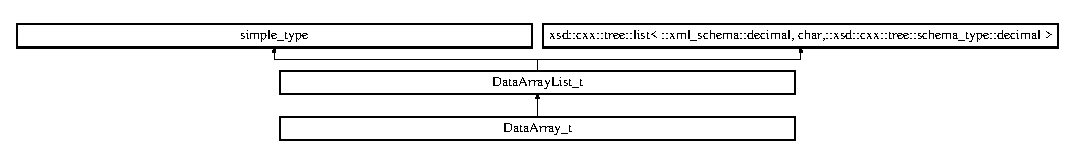
\includegraphics[height=1.660079cm]{classDataArray__t}
\end{center}
\end{figure}
\subsection*{Public Types}
\begin{DoxyCompactItemize}
\item 
typedef \+::\hyperlink{classtype}{type} \hyperlink{classDataArray__t_a484a0509e4f141d9970d75881703a51e}{type\+\_\+type}
\item 
typedef \+::xsd\+::cxx\+::tree\+::traits$<$ \hyperlink{classDataArray__t_a484a0509e4f141d9970d75881703a51e}{type\+\_\+type}, char $>$ \hyperlink{classDataArray__t_af1dc5f097a8645ae42b57eb3a0b10fa2}{type\+\_\+traits}
\item 
typedef \+::\hyperlink{namespacexml__schema_ac0cec83a330f0024e4e318b3deac5104}{xml\+\_\+schema\+::string} \hyperlink{classDataArray__t_afc6836923916c2489f91caea78ec4ad6}{Name\+\_\+type}
\item 
typedef \+::xsd\+::cxx\+::tree\+::traits$<$ \hyperlink{classDataArray__t_afc6836923916c2489f91caea78ec4ad6}{Name\+\_\+type}, char $>$ \hyperlink{classDataArray__t_a46d0b4cf44ee9122e4cbb3bd3abe6663}{Name\+\_\+traits}
\item 
typedef \+::\hyperlink{namespacexml__schema_aaaea7c8ce4dfbe26cc52c91c29c97b7c}{xml\+\_\+schema\+::integer} \hyperlink{classDataArray__t_aac602cec132f6e771f7fa3be1d19c16f}{Number\+Of\+Components\+\_\+type}
\item 
typedef \+::xsd\+::cxx\+::tree\+::traits$<$ \hyperlink{classDataArray__t_aac602cec132f6e771f7fa3be1d19c16f}{Number\+Of\+Components\+\_\+type}, char $>$ \hyperlink{classDataArray__t_a1112148f87db2c0ba05323377d9f0427}{Number\+Of\+Components\+\_\+traits}
\item 
typedef \+::\hyperlink{namespacexml__schema_ac0cec83a330f0024e4e318b3deac5104}{xml\+\_\+schema\+::string} \hyperlink{classDataArray__t_ae453ea653980baef2e3296005d70bfbd}{format\+\_\+type}
\item 
typedef \+::xsd\+::cxx\+::tree\+::traits$<$ \hyperlink{classDataArray__t_ae453ea653980baef2e3296005d70bfbd}{format\+\_\+type}, char $>$ \hyperlink{classDataArray__t_a2a31ef3ce1dfa973843a02e17762e7a3}{format\+\_\+traits}
\item 
typedef \+::\hyperlink{namespacexml__schema_aaaea7c8ce4dfbe26cc52c91c29c97b7c}{xml\+\_\+schema\+::integer} \hyperlink{classDataArray__t_a7b840c5f08bd2c65cd3c5e24ad132cfb}{offset\+\_\+type}
\item 
typedef \+::xsd\+::cxx\+::tree\+::optional$<$ \hyperlink{classDataArray__t_a7b840c5f08bd2c65cd3c5e24ad132cfb}{offset\+\_\+type} $>$ \hyperlink{classDataArray__t_a4bc33060e7c386b658c752347ac5f03e}{offset\+\_\+optional}
\item 
typedef \+::xsd\+::cxx\+::tree\+::traits$<$ \hyperlink{classDataArray__t_a7b840c5f08bd2c65cd3c5e24ad132cfb}{offset\+\_\+type}, char $>$ \hyperlink{classDataArray__t_a2e3e1a5de665fc64a3d86fd94bb1af0f}{offset\+\_\+traits}
\end{DoxyCompactItemize}
\subsection*{Public Member Functions}
\begin{DoxyCompactItemize}
\item 
const \hyperlink{classDataArray__t_a484a0509e4f141d9970d75881703a51e}{type\+\_\+type} \& \hyperlink{classDataArray__t_a6ec3c246d1a2fddc7052bcde2cb6bdf7}{type} () const 
\item 
\hyperlink{classDataArray__t_a484a0509e4f141d9970d75881703a51e}{type\+\_\+type} \& \hyperlink{classDataArray__t_a29f3ed42a5bf8df9437ece5f63c02301}{type} ()
\item 
void \hyperlink{classDataArray__t_ae4fd6c47e992055ec42cc1949b60da2a}{type} (const \hyperlink{classDataArray__t_a484a0509e4f141d9970d75881703a51e}{type\+\_\+type} \&x)
\item 
void \hyperlink{classDataArray__t_a271b76368e9e5331b27c896a7ce9dda7}{type} (\+::std\+::unique\+\_\+ptr$<$ \hyperlink{classDataArray__t_a484a0509e4f141d9970d75881703a51e}{type\+\_\+type} $>$ p)
\item 
const \hyperlink{classDataArray__t_afc6836923916c2489f91caea78ec4ad6}{Name\+\_\+type} \& \hyperlink{classDataArray__t_ada03ebff820f73d64d0761a0fb977527}{Name} () const 
\item 
\hyperlink{classDataArray__t_afc6836923916c2489f91caea78ec4ad6}{Name\+\_\+type} \& \hyperlink{classDataArray__t_aeb126f8a8b03eea44eed5a2b606da59c}{Name} ()
\item 
void \hyperlink{classDataArray__t_a95a1f49a6dd9f54fb71fb6b70240a51b}{Name} (const \hyperlink{classDataArray__t_afc6836923916c2489f91caea78ec4ad6}{Name\+\_\+type} \&x)
\item 
void \hyperlink{classDataArray__t_add3007d3bd0cecaf0800c20c297373ec}{Name} (\+::std\+::unique\+\_\+ptr$<$ \hyperlink{classDataArray__t_afc6836923916c2489f91caea78ec4ad6}{Name\+\_\+type} $>$ p)
\item 
const \hyperlink{classDataArray__t_aac602cec132f6e771f7fa3be1d19c16f}{Number\+Of\+Components\+\_\+type} \& \hyperlink{classDataArray__t_a715a5b58a694d49499591bfea3a282ae}{Number\+Of\+Components} () const 
\item 
\hyperlink{classDataArray__t_aac602cec132f6e771f7fa3be1d19c16f}{Number\+Of\+Components\+\_\+type} \& \hyperlink{classDataArray__t_a6f80fc5ce05d51d4292c698464d4ace3}{Number\+Of\+Components} ()
\item 
void \hyperlink{classDataArray__t_a755fae9b31318f98a3d21beba16f2841}{Number\+Of\+Components} (const \hyperlink{classDataArray__t_aac602cec132f6e771f7fa3be1d19c16f}{Number\+Of\+Components\+\_\+type} \&x)
\item 
const \hyperlink{classDataArray__t_ae453ea653980baef2e3296005d70bfbd}{format\+\_\+type} \& \hyperlink{classDataArray__t_a7a39cab4205282736e633d8a3c57bbae}{format} () const 
\item 
const \hyperlink{classDataArray__t_a4bc33060e7c386b658c752347ac5f03e}{offset\+\_\+optional} \& \hyperlink{classDataArray__t_a995d24c5c7a88929a6b0e7de154bbdf5}{offset} () const 
\item 
\hyperlink{classDataArray__t_a4bc33060e7c386b658c752347ac5f03e}{offset\+\_\+optional} \& \hyperlink{classDataArray__t_aed72cbf5f3476360f4898f487a074c26}{offset} ()
\item 
void \hyperlink{classDataArray__t_ac133def4ed8ae6c623d0144f036a18d7}{offset} (const \hyperlink{classDataArray__t_a7b840c5f08bd2c65cd3c5e24ad132cfb}{offset\+\_\+type} \&x)
\item 
void \hyperlink{classDataArray__t_a5abb95d7ab6fb95015c06de57a6ccbc9}{offset} (const \hyperlink{classDataArray__t_a4bc33060e7c386b658c752347ac5f03e}{offset\+\_\+optional} \&x)
\item 
\hyperlink{classDataArray__t_a0700e9e63538064c2f9eb668fe3ca624}{Data\+Array\+\_\+t} (const \hyperlink{classDataArray__t_a484a0509e4f141d9970d75881703a51e}{type\+\_\+type} \&, const \hyperlink{classDataArray__t_afc6836923916c2489f91caea78ec4ad6}{Name\+\_\+type} \&, const \hyperlink{classDataArray__t_aac602cec132f6e771f7fa3be1d19c16f}{Number\+Of\+Components\+\_\+type} \&)
\item 
\hyperlink{classDataArray__t_a3c07c46f9c607ce6da2d2e456494465a}{Data\+Array\+\_\+t} (const \+::\hyperlink{classDataArrayList__t}{Data\+Array\+List\+\_\+t} \&, const \hyperlink{classDataArray__t_a484a0509e4f141d9970d75881703a51e}{type\+\_\+type} \&, const \hyperlink{classDataArray__t_afc6836923916c2489f91caea78ec4ad6}{Name\+\_\+type} \&, const \hyperlink{classDataArray__t_aac602cec132f6e771f7fa3be1d19c16f}{Number\+Of\+Components\+\_\+type} \&)
\item 
\hyperlink{classDataArray__t_ae02d07853318c1d754e0acfc80f5c894}{Data\+Array\+\_\+t} (const \+::xercesc\+::\+D\+O\+M\+Element \&e,\+::\hyperlink{namespacexml__schema_a0612287d030cb2732d31a45b258fdc87}{xml\+\_\+schema\+::flags} f=0,\+::\hyperlink{namespacexml__schema_ada9aa30dc722e93ee2ed7243085402a5}{xml\+\_\+schema\+::container} $\ast$c=0)
\item 
\hyperlink{classDataArray__t_a6f67fee4225ca87492d8496de4121de7}{Data\+Array\+\_\+t} (const \hyperlink{classDataArray__t}{Data\+Array\+\_\+t} \&x,\+::\hyperlink{namespacexml__schema_a0612287d030cb2732d31a45b258fdc87}{xml\+\_\+schema\+::flags} f=0,\+::\hyperlink{namespacexml__schema_ada9aa30dc722e93ee2ed7243085402a5}{xml\+\_\+schema\+::container} $\ast$c=0)
\item 
virtual \hyperlink{classDataArray__t}{Data\+Array\+\_\+t} $\ast$ \hyperlink{classDataArray__t_a0ba3569846912b9fcadbd942e914cce1}{\+\_\+clone} (\+::\hyperlink{namespacexml__schema_a0612287d030cb2732d31a45b258fdc87}{xml\+\_\+schema\+::flags} f=0,\+::\hyperlink{namespacexml__schema_ada9aa30dc722e93ee2ed7243085402a5}{xml\+\_\+schema\+::container} $\ast$c=0) const 
\item 
\hyperlink{classDataArray__t}{Data\+Array\+\_\+t} \& \hyperlink{classDataArray__t_acaa5dfa86244de30a94634a9430e0f2d}{operator=} (const \hyperlink{classDataArray__t}{Data\+Array\+\_\+t} \&x)
\item 
virtual \hyperlink{classDataArray__t_ac9806a5eedf7abecd7adf6408c8af894}{$\sim$\+Data\+Array\+\_\+t} ()
\end{DoxyCompactItemize}
\subsection*{Static Public Member Functions}
\begin{DoxyCompactItemize}
\item 
static const \hyperlink{classDataArray__t_ae453ea653980baef2e3296005d70bfbd}{format\+\_\+type} \& \hyperlink{classDataArray__t_ade99ea2c2fdc45cc2826b6847dfb5404}{format\+\_\+default\+\_\+value} ()
\end{DoxyCompactItemize}
\subsection*{Protected Member Functions}
\begin{DoxyCompactItemize}
\item 
void \hyperlink{classDataArray__t_a08396be94c9f535e1d8e7c68941f7833}{parse} (\+::xsd\+::cxx\+::xml\+::dom\+::parser$<$ char $>$ \&,\+::\hyperlink{namespacexml__schema_a0612287d030cb2732d31a45b258fdc87}{xml\+\_\+schema\+::flags})
\end{DoxyCompactItemize}
\subsection*{Protected Attributes}
\begin{DoxyCompactItemize}
\item 
\+::xsd\+::cxx\+::tree\+::one$<$ \hyperlink{classDataArray__t_a484a0509e4f141d9970d75881703a51e}{type\+\_\+type} $>$ \hyperlink{classDataArray__t_a213841b0371a05383d0de7b8cf35c571}{type\+\_\+}
\item 
\+::xsd\+::cxx\+::tree\+::one$<$ \hyperlink{classDataArray__t_afc6836923916c2489f91caea78ec4ad6}{Name\+\_\+type} $>$ \hyperlink{classDataArray__t_a75c5be79f9202ea631b90bc7ab6572ac}{Name\+\_\+}
\item 
\+::xsd\+::cxx\+::tree\+::one$<$ \hyperlink{classDataArray__t_aac602cec132f6e771f7fa3be1d19c16f}{Number\+Of\+Components\+\_\+type} $>$ \hyperlink{classDataArray__t_ae0e1c29893204a5066b86ffe5101d176}{Number\+Of\+Components\+\_\+}
\item 
\+::xsd\+::cxx\+::tree\+::one$<$ \hyperlink{classDataArray__t_ae453ea653980baef2e3296005d70bfbd}{format\+\_\+type} $>$ \hyperlink{classDataArray__t_a96cef5bd78a9f11079aa5dfe94d7b540}{format\+\_\+}
\item 
\hyperlink{classDataArray__t_a4bc33060e7c386b658c752347ac5f03e}{offset\+\_\+optional} \hyperlink{classDataArray__t_a6479c8a02a37c84956afb645b247ef0e}{offset\+\_\+}
\end{DoxyCompactItemize}
\subsection*{Static Protected Attributes}
\begin{DoxyCompactItemize}
\item 
static const \hyperlink{classDataArray__t_ae453ea653980baef2e3296005d70bfbd}{format\+\_\+type} \hyperlink{classDataArray__t_ab96d3bb715c0ac4b96279a85eef117a8}{format\+\_\+default\+\_\+value\+\_\+}
\end{DoxyCompactItemize}


\subsection{Member Typedef Documentation}
\index{Data\+Array\+\_\+t@{Data\+Array\+\_\+t}!format\+\_\+traits@{format\+\_\+traits}}
\index{format\+\_\+traits@{format\+\_\+traits}!Data\+Array\+\_\+t@{Data\+Array\+\_\+t}}
\subsubsection[{\texorpdfstring{format\+\_\+traits}{format_traits}}]{\setlength{\rightskip}{0pt plus 5cm}typedef \+::xsd\+::cxx\+::tree\+::traits$<$ {\bf format\+\_\+type}, char $>$ {\bf Data\+Array\+\_\+t\+::format\+\_\+traits}}\hypertarget{classDataArray__t_a2a31ef3ce1dfa973843a02e17762e7a3}{}\label{classDataArray__t_a2a31ef3ce1dfa973843a02e17762e7a3}
\index{Data\+Array\+\_\+t@{Data\+Array\+\_\+t}!format\+\_\+type@{format\+\_\+type}}
\index{format\+\_\+type@{format\+\_\+type}!Data\+Array\+\_\+t@{Data\+Array\+\_\+t}}
\subsubsection[{\texorpdfstring{format\+\_\+type}{format_type}}]{\setlength{\rightskip}{0pt plus 5cm}typedef \+::{\bf xml\+\_\+schema\+::string} {\bf Data\+Array\+\_\+t\+::format\+\_\+type}}\hypertarget{classDataArray__t_ae453ea653980baef2e3296005d70bfbd}{}\label{classDataArray__t_ae453ea653980baef2e3296005d70bfbd}
\index{Data\+Array\+\_\+t@{Data\+Array\+\_\+t}!Name\+\_\+traits@{Name\+\_\+traits}}
\index{Name\+\_\+traits@{Name\+\_\+traits}!Data\+Array\+\_\+t@{Data\+Array\+\_\+t}}
\subsubsection[{\texorpdfstring{Name\+\_\+traits}{Name_traits}}]{\setlength{\rightskip}{0pt plus 5cm}typedef \+::xsd\+::cxx\+::tree\+::traits$<$ {\bf Name\+\_\+type}, char $>$ {\bf Data\+Array\+\_\+t\+::\+Name\+\_\+traits}}\hypertarget{classDataArray__t_a46d0b4cf44ee9122e4cbb3bd3abe6663}{}\label{classDataArray__t_a46d0b4cf44ee9122e4cbb3bd3abe6663}
\index{Data\+Array\+\_\+t@{Data\+Array\+\_\+t}!Name\+\_\+type@{Name\+\_\+type}}
\index{Name\+\_\+type@{Name\+\_\+type}!Data\+Array\+\_\+t@{Data\+Array\+\_\+t}}
\subsubsection[{\texorpdfstring{Name\+\_\+type}{Name_type}}]{\setlength{\rightskip}{0pt plus 5cm}typedef \+::{\bf xml\+\_\+schema\+::string} {\bf Data\+Array\+\_\+t\+::\+Name\+\_\+type}}\hypertarget{classDataArray__t_afc6836923916c2489f91caea78ec4ad6}{}\label{classDataArray__t_afc6836923916c2489f91caea78ec4ad6}
\index{Data\+Array\+\_\+t@{Data\+Array\+\_\+t}!Number\+Of\+Components\+\_\+traits@{Number\+Of\+Components\+\_\+traits}}
\index{Number\+Of\+Components\+\_\+traits@{Number\+Of\+Components\+\_\+traits}!Data\+Array\+\_\+t@{Data\+Array\+\_\+t}}
\subsubsection[{\texorpdfstring{Number\+Of\+Components\+\_\+traits}{NumberOfComponents_traits}}]{\setlength{\rightskip}{0pt plus 5cm}typedef \+::xsd\+::cxx\+::tree\+::traits$<$ {\bf Number\+Of\+Components\+\_\+type}, char $>$ {\bf Data\+Array\+\_\+t\+::\+Number\+Of\+Components\+\_\+traits}}\hypertarget{classDataArray__t_a1112148f87db2c0ba05323377d9f0427}{}\label{classDataArray__t_a1112148f87db2c0ba05323377d9f0427}
\index{Data\+Array\+\_\+t@{Data\+Array\+\_\+t}!Number\+Of\+Components\+\_\+type@{Number\+Of\+Components\+\_\+type}}
\index{Number\+Of\+Components\+\_\+type@{Number\+Of\+Components\+\_\+type}!Data\+Array\+\_\+t@{Data\+Array\+\_\+t}}
\subsubsection[{\texorpdfstring{Number\+Of\+Components\+\_\+type}{NumberOfComponents_type}}]{\setlength{\rightskip}{0pt plus 5cm}typedef \+::{\bf xml\+\_\+schema\+::integer} {\bf Data\+Array\+\_\+t\+::\+Number\+Of\+Components\+\_\+type}}\hypertarget{classDataArray__t_aac602cec132f6e771f7fa3be1d19c16f}{}\label{classDataArray__t_aac602cec132f6e771f7fa3be1d19c16f}
\index{Data\+Array\+\_\+t@{Data\+Array\+\_\+t}!offset\+\_\+optional@{offset\+\_\+optional}}
\index{offset\+\_\+optional@{offset\+\_\+optional}!Data\+Array\+\_\+t@{Data\+Array\+\_\+t}}
\subsubsection[{\texorpdfstring{offset\+\_\+optional}{offset_optional}}]{\setlength{\rightskip}{0pt plus 5cm}typedef \+::xsd\+::cxx\+::tree\+::optional$<$ {\bf offset\+\_\+type} $>$ {\bf Data\+Array\+\_\+t\+::offset\+\_\+optional}}\hypertarget{classDataArray__t_a4bc33060e7c386b658c752347ac5f03e}{}\label{classDataArray__t_a4bc33060e7c386b658c752347ac5f03e}
\index{Data\+Array\+\_\+t@{Data\+Array\+\_\+t}!offset\+\_\+traits@{offset\+\_\+traits}}
\index{offset\+\_\+traits@{offset\+\_\+traits}!Data\+Array\+\_\+t@{Data\+Array\+\_\+t}}
\subsubsection[{\texorpdfstring{offset\+\_\+traits}{offset_traits}}]{\setlength{\rightskip}{0pt plus 5cm}typedef \+::xsd\+::cxx\+::tree\+::traits$<$ {\bf offset\+\_\+type}, char $>$ {\bf Data\+Array\+\_\+t\+::offset\+\_\+traits}}\hypertarget{classDataArray__t_a2e3e1a5de665fc64a3d86fd94bb1af0f}{}\label{classDataArray__t_a2e3e1a5de665fc64a3d86fd94bb1af0f}
\index{Data\+Array\+\_\+t@{Data\+Array\+\_\+t}!offset\+\_\+type@{offset\+\_\+type}}
\index{offset\+\_\+type@{offset\+\_\+type}!Data\+Array\+\_\+t@{Data\+Array\+\_\+t}}
\subsubsection[{\texorpdfstring{offset\+\_\+type}{offset_type}}]{\setlength{\rightskip}{0pt plus 5cm}typedef \+::{\bf xml\+\_\+schema\+::integer} {\bf Data\+Array\+\_\+t\+::offset\+\_\+type}}\hypertarget{classDataArray__t_a7b840c5f08bd2c65cd3c5e24ad132cfb}{}\label{classDataArray__t_a7b840c5f08bd2c65cd3c5e24ad132cfb}
\index{Data\+Array\+\_\+t@{Data\+Array\+\_\+t}!type\+\_\+traits@{type\+\_\+traits}}
\index{type\+\_\+traits@{type\+\_\+traits}!Data\+Array\+\_\+t@{Data\+Array\+\_\+t}}
\subsubsection[{\texorpdfstring{type\+\_\+traits}{type_traits}}]{\setlength{\rightskip}{0pt plus 5cm}typedef \+::xsd\+::cxx\+::tree\+::traits$<$ {\bf type\+\_\+type}, char $>$ {\bf Data\+Array\+\_\+t\+::type\+\_\+traits}}\hypertarget{classDataArray__t_af1dc5f097a8645ae42b57eb3a0b10fa2}{}\label{classDataArray__t_af1dc5f097a8645ae42b57eb3a0b10fa2}
\index{Data\+Array\+\_\+t@{Data\+Array\+\_\+t}!type\+\_\+type@{type\+\_\+type}}
\index{type\+\_\+type@{type\+\_\+type}!Data\+Array\+\_\+t@{Data\+Array\+\_\+t}}
\subsubsection[{\texorpdfstring{type\+\_\+type}{type_type}}]{\setlength{\rightskip}{0pt plus 5cm}typedef \+::{\bf type} {\bf Data\+Array\+\_\+t\+::type\+\_\+type}}\hypertarget{classDataArray__t_a484a0509e4f141d9970d75881703a51e}{}\label{classDataArray__t_a484a0509e4f141d9970d75881703a51e}


\subsection{Constructor \& Destructor Documentation}
\index{Data\+Array\+\_\+t@{Data\+Array\+\_\+t}!Data\+Array\+\_\+t@{Data\+Array\+\_\+t}}
\index{Data\+Array\+\_\+t@{Data\+Array\+\_\+t}!Data\+Array\+\_\+t@{Data\+Array\+\_\+t}}
\subsubsection[{\texorpdfstring{Data\+Array\+\_\+t(const type\+\_\+type \&, const Name\+\_\+type \&, const Number\+Of\+Components\+\_\+type \&)}{DataArray_t(const type_type &, const Name_type &, const NumberOfComponents_type &)}}]{\setlength{\rightskip}{0pt plus 5cm}Data\+Array\+\_\+t\+::\+Data\+Array\+\_\+t (
\begin{DoxyParamCaption}
\item[{const {\bf type\+\_\+type} \&}]{type, }
\item[{const {\bf Name\+\_\+type} \&}]{Name, }
\item[{const {\bf Number\+Of\+Components\+\_\+type} \&}]{Number\+Of\+Components}
\end{DoxyParamCaption}
)}\hypertarget{classDataArray__t_a0700e9e63538064c2f9eb668fe3ca624}{}\label{classDataArray__t_a0700e9e63538064c2f9eb668fe3ca624}
\index{Data\+Array\+\_\+t@{Data\+Array\+\_\+t}!Data\+Array\+\_\+t@{Data\+Array\+\_\+t}}
\index{Data\+Array\+\_\+t@{Data\+Array\+\_\+t}!Data\+Array\+\_\+t@{Data\+Array\+\_\+t}}
\subsubsection[{\texorpdfstring{Data\+Array\+\_\+t(const \+::\+Data\+Array\+List\+\_\+t \&, const type\+\_\+type \&, const Name\+\_\+type \&, const Number\+Of\+Components\+\_\+type \&)}{DataArray_t(const ::DataArrayList_t &, const type_type &, const Name_type &, const NumberOfComponents_type &)}}]{\setlength{\rightskip}{0pt plus 5cm}Data\+Array\+\_\+t\+::\+Data\+Array\+\_\+t (
\begin{DoxyParamCaption}
\item[{const \+::{\bf Data\+Array\+List\+\_\+t} \&}]{\+\_\+xsd\+\_\+\+Data\+Array\+List\+\_\+t\+\_\+base, }
\item[{const {\bf type\+\_\+type} \&}]{type, }
\item[{const {\bf Name\+\_\+type} \&}]{Name, }
\item[{const {\bf Number\+Of\+Components\+\_\+type} \&}]{Number\+Of\+Components}
\end{DoxyParamCaption}
)}\hypertarget{classDataArray__t_a3c07c46f9c607ce6da2d2e456494465a}{}\label{classDataArray__t_a3c07c46f9c607ce6da2d2e456494465a}
\index{Data\+Array\+\_\+t@{Data\+Array\+\_\+t}!Data\+Array\+\_\+t@{Data\+Array\+\_\+t}}
\index{Data\+Array\+\_\+t@{Data\+Array\+\_\+t}!Data\+Array\+\_\+t@{Data\+Array\+\_\+t}}
\subsubsection[{\texorpdfstring{Data\+Array\+\_\+t(const \+::xercesc\+::\+D\+O\+M\+Element \&e,\+::xml\+\_\+schema\+::flags f=0,\+::xml\+\_\+schema\+::container $\ast$c=0)}{DataArray_t(const ::xercesc::DOMElement &e,::xml_schema::flags f=0,::xml_schema::container *c=0)}}]{\setlength{\rightskip}{0pt plus 5cm}Data\+Array\+\_\+t\+::\+Data\+Array\+\_\+t (
\begin{DoxyParamCaption}
\item[{const \+::xercesc\+::\+D\+O\+M\+Element \&}]{e, }
\item[{\+::{\bf xml\+\_\+schema\+::flags}}]{f = {\ttfamily 0}, }
\item[{\+::{\bf xml\+\_\+schema\+::container} $\ast$}]{c = {\ttfamily 0}}
\end{DoxyParamCaption}
)}\hypertarget{classDataArray__t_ae02d07853318c1d754e0acfc80f5c894}{}\label{classDataArray__t_ae02d07853318c1d754e0acfc80f5c894}
\index{Data\+Array\+\_\+t@{Data\+Array\+\_\+t}!Data\+Array\+\_\+t@{Data\+Array\+\_\+t}}
\index{Data\+Array\+\_\+t@{Data\+Array\+\_\+t}!Data\+Array\+\_\+t@{Data\+Array\+\_\+t}}
\subsubsection[{\texorpdfstring{Data\+Array\+\_\+t(const Data\+Array\+\_\+t \&x,\+::xml\+\_\+schema\+::flags f=0,\+::xml\+\_\+schema\+::container $\ast$c=0)}{DataArray_t(const DataArray_t &x,::xml_schema::flags f=0,::xml_schema::container *c=0)}}]{\setlength{\rightskip}{0pt plus 5cm}Data\+Array\+\_\+t\+::\+Data\+Array\+\_\+t (
\begin{DoxyParamCaption}
\item[{const {\bf Data\+Array\+\_\+t} \&}]{x, }
\item[{\+::{\bf xml\+\_\+schema\+::flags}}]{f = {\ttfamily 0}, }
\item[{\+::{\bf xml\+\_\+schema\+::container} $\ast$}]{c = {\ttfamily 0}}
\end{DoxyParamCaption}
)}\hypertarget{classDataArray__t_a6f67fee4225ca87492d8496de4121de7}{}\label{classDataArray__t_a6f67fee4225ca87492d8496de4121de7}
\index{Data\+Array\+\_\+t@{Data\+Array\+\_\+t}!````~Data\+Array\+\_\+t@{$\sim$\+Data\+Array\+\_\+t}}
\index{````~Data\+Array\+\_\+t@{$\sim$\+Data\+Array\+\_\+t}!Data\+Array\+\_\+t@{Data\+Array\+\_\+t}}
\subsubsection[{\texorpdfstring{$\sim$\+Data\+Array\+\_\+t()}{~DataArray_t()}}]{\setlength{\rightskip}{0pt plus 5cm}Data\+Array\+\_\+t\+::$\sim$\+Data\+Array\+\_\+t (
\begin{DoxyParamCaption}
{}
\end{DoxyParamCaption}
)\hspace{0.3cm}{\ttfamily [virtual]}}\hypertarget{classDataArray__t_ac9806a5eedf7abecd7adf6408c8af894}{}\label{classDataArray__t_ac9806a5eedf7abecd7adf6408c8af894}


\subsection{Member Function Documentation}
\index{Data\+Array\+\_\+t@{Data\+Array\+\_\+t}!\+\_\+clone@{\+\_\+clone}}
\index{\+\_\+clone@{\+\_\+clone}!Data\+Array\+\_\+t@{Data\+Array\+\_\+t}}
\subsubsection[{\texorpdfstring{\+\_\+clone(\+::xml\+\_\+schema\+::flags f=0,\+::xml\+\_\+schema\+::container $\ast$c=0) const }{_clone(::xml_schema::flags f=0,::xml_schema::container *c=0) const }}]{\setlength{\rightskip}{0pt plus 5cm}{\bf Data\+Array\+\_\+t} $\ast$ Data\+Array\+\_\+t\+::\+\_\+clone (
\begin{DoxyParamCaption}
\item[{\+::{\bf xml\+\_\+schema\+::flags}}]{f = {\ttfamily 0}, }
\item[{\+::{\bf xml\+\_\+schema\+::container} $\ast$}]{c = {\ttfamily 0}}
\end{DoxyParamCaption}
) const\hspace{0.3cm}{\ttfamily [virtual]}}\hypertarget{classDataArray__t_a0ba3569846912b9fcadbd942e914cce1}{}\label{classDataArray__t_a0ba3569846912b9fcadbd942e914cce1}


Reimplemented from \hyperlink{classDataArrayList__t_acec29e88488ded1352c5b064827f5c38}{Data\+Array\+List\+\_\+t}.

\index{Data\+Array\+\_\+t@{Data\+Array\+\_\+t}!format@{format}}
\index{format@{format}!Data\+Array\+\_\+t@{Data\+Array\+\_\+t}}
\subsubsection[{\texorpdfstring{format() const }{format() const }}]{\setlength{\rightskip}{0pt plus 5cm}const {\bf Data\+Array\+\_\+t\+::format\+\_\+type} \& Data\+Array\+\_\+t\+::format (
\begin{DoxyParamCaption}
{}
\end{DoxyParamCaption}
) const}\hypertarget{classDataArray__t_a7a39cab4205282736e633d8a3c57bbae}{}\label{classDataArray__t_a7a39cab4205282736e633d8a3c57bbae}
\index{Data\+Array\+\_\+t@{Data\+Array\+\_\+t}!format\+\_\+default\+\_\+value@{format\+\_\+default\+\_\+value}}
\index{format\+\_\+default\+\_\+value@{format\+\_\+default\+\_\+value}!Data\+Array\+\_\+t@{Data\+Array\+\_\+t}}
\subsubsection[{\texorpdfstring{format\+\_\+default\+\_\+value()}{format_default_value()}}]{\setlength{\rightskip}{0pt plus 5cm}const {\bf Data\+Array\+\_\+t\+::format\+\_\+type} \& Data\+Array\+\_\+t\+::format\+\_\+default\+\_\+value (
\begin{DoxyParamCaption}
{}
\end{DoxyParamCaption}
)\hspace{0.3cm}{\ttfamily [static]}}\hypertarget{classDataArray__t_ade99ea2c2fdc45cc2826b6847dfb5404}{}\label{classDataArray__t_ade99ea2c2fdc45cc2826b6847dfb5404}
\index{Data\+Array\+\_\+t@{Data\+Array\+\_\+t}!Name@{Name}}
\index{Name@{Name}!Data\+Array\+\_\+t@{Data\+Array\+\_\+t}}
\subsubsection[{\texorpdfstring{Name() const }{Name() const }}]{\setlength{\rightskip}{0pt plus 5cm}const {\bf Data\+Array\+\_\+t\+::\+Name\+\_\+type} \& Data\+Array\+\_\+t\+::\+Name (
\begin{DoxyParamCaption}
{}
\end{DoxyParamCaption}
) const}\hypertarget{classDataArray__t_ada03ebff820f73d64d0761a0fb977527}{}\label{classDataArray__t_ada03ebff820f73d64d0761a0fb977527}
\index{Data\+Array\+\_\+t@{Data\+Array\+\_\+t}!Name@{Name}}
\index{Name@{Name}!Data\+Array\+\_\+t@{Data\+Array\+\_\+t}}
\subsubsection[{\texorpdfstring{Name()}{Name()}}]{\setlength{\rightskip}{0pt plus 5cm}{\bf Data\+Array\+\_\+t\+::\+Name\+\_\+type} \& Data\+Array\+\_\+t\+::\+Name (
\begin{DoxyParamCaption}
{}
\end{DoxyParamCaption}
)}\hypertarget{classDataArray__t_aeb126f8a8b03eea44eed5a2b606da59c}{}\label{classDataArray__t_aeb126f8a8b03eea44eed5a2b606da59c}
\index{Data\+Array\+\_\+t@{Data\+Array\+\_\+t}!Name@{Name}}
\index{Name@{Name}!Data\+Array\+\_\+t@{Data\+Array\+\_\+t}}
\subsubsection[{\texorpdfstring{Name(const Name\+\_\+type \&x)}{Name(const Name_type &x)}}]{\setlength{\rightskip}{0pt plus 5cm}void Data\+Array\+\_\+t\+::\+Name (
\begin{DoxyParamCaption}
\item[{const {\bf Name\+\_\+type} \&}]{x}
\end{DoxyParamCaption}
)}\hypertarget{classDataArray__t_a95a1f49a6dd9f54fb71fb6b70240a51b}{}\label{classDataArray__t_a95a1f49a6dd9f54fb71fb6b70240a51b}
\index{Data\+Array\+\_\+t@{Data\+Array\+\_\+t}!Name@{Name}}
\index{Name@{Name}!Data\+Array\+\_\+t@{Data\+Array\+\_\+t}}
\subsubsection[{\texorpdfstring{Name(\+::std\+::unique\+\_\+ptr$<$ Name\+\_\+type $>$ p)}{Name(::std::unique_ptr< Name_type > p)}}]{\setlength{\rightskip}{0pt plus 5cm}void Data\+Array\+\_\+t\+::\+Name (
\begin{DoxyParamCaption}
\item[{\+::std\+::unique\+\_\+ptr$<$ {\bf Name\+\_\+type} $>$}]{p}
\end{DoxyParamCaption}
)}\hypertarget{classDataArray__t_add3007d3bd0cecaf0800c20c297373ec}{}\label{classDataArray__t_add3007d3bd0cecaf0800c20c297373ec}
\index{Data\+Array\+\_\+t@{Data\+Array\+\_\+t}!Number\+Of\+Components@{Number\+Of\+Components}}
\index{Number\+Of\+Components@{Number\+Of\+Components}!Data\+Array\+\_\+t@{Data\+Array\+\_\+t}}
\subsubsection[{\texorpdfstring{Number\+Of\+Components() const }{NumberOfComponents() const }}]{\setlength{\rightskip}{0pt plus 5cm}const {\bf Data\+Array\+\_\+t\+::\+Number\+Of\+Components\+\_\+type} \& Data\+Array\+\_\+t\+::\+Number\+Of\+Components (
\begin{DoxyParamCaption}
{}
\end{DoxyParamCaption}
) const}\hypertarget{classDataArray__t_a715a5b58a694d49499591bfea3a282ae}{}\label{classDataArray__t_a715a5b58a694d49499591bfea3a282ae}
\index{Data\+Array\+\_\+t@{Data\+Array\+\_\+t}!Number\+Of\+Components@{Number\+Of\+Components}}
\index{Number\+Of\+Components@{Number\+Of\+Components}!Data\+Array\+\_\+t@{Data\+Array\+\_\+t}}
\subsubsection[{\texorpdfstring{Number\+Of\+Components()}{NumberOfComponents()}}]{\setlength{\rightskip}{0pt plus 5cm}{\bf Data\+Array\+\_\+t\+::\+Number\+Of\+Components\+\_\+type} \& Data\+Array\+\_\+t\+::\+Number\+Of\+Components (
\begin{DoxyParamCaption}
{}
\end{DoxyParamCaption}
)}\hypertarget{classDataArray__t_a6f80fc5ce05d51d4292c698464d4ace3}{}\label{classDataArray__t_a6f80fc5ce05d51d4292c698464d4ace3}
\index{Data\+Array\+\_\+t@{Data\+Array\+\_\+t}!Number\+Of\+Components@{Number\+Of\+Components}}
\index{Number\+Of\+Components@{Number\+Of\+Components}!Data\+Array\+\_\+t@{Data\+Array\+\_\+t}}
\subsubsection[{\texorpdfstring{Number\+Of\+Components(const Number\+Of\+Components\+\_\+type \&x)}{NumberOfComponents(const NumberOfComponents_type &x)}}]{\setlength{\rightskip}{0pt plus 5cm}void Data\+Array\+\_\+t\+::\+Number\+Of\+Components (
\begin{DoxyParamCaption}
\item[{const {\bf Number\+Of\+Components\+\_\+type} \&}]{x}
\end{DoxyParamCaption}
)}\hypertarget{classDataArray__t_a755fae9b31318f98a3d21beba16f2841}{}\label{classDataArray__t_a755fae9b31318f98a3d21beba16f2841}
\index{Data\+Array\+\_\+t@{Data\+Array\+\_\+t}!offset@{offset}}
\index{offset@{offset}!Data\+Array\+\_\+t@{Data\+Array\+\_\+t}}
\subsubsection[{\texorpdfstring{offset() const }{offset() const }}]{\setlength{\rightskip}{0pt plus 5cm}const {\bf Data\+Array\+\_\+t\+::offset\+\_\+optional} \& Data\+Array\+\_\+t\+::offset (
\begin{DoxyParamCaption}
{}
\end{DoxyParamCaption}
) const}\hypertarget{classDataArray__t_a995d24c5c7a88929a6b0e7de154bbdf5}{}\label{classDataArray__t_a995d24c5c7a88929a6b0e7de154bbdf5}
\index{Data\+Array\+\_\+t@{Data\+Array\+\_\+t}!offset@{offset}}
\index{offset@{offset}!Data\+Array\+\_\+t@{Data\+Array\+\_\+t}}
\subsubsection[{\texorpdfstring{offset()}{offset()}}]{\setlength{\rightskip}{0pt plus 5cm}{\bf Data\+Array\+\_\+t\+::offset\+\_\+optional} \& Data\+Array\+\_\+t\+::offset (
\begin{DoxyParamCaption}
{}
\end{DoxyParamCaption}
)}\hypertarget{classDataArray__t_aed72cbf5f3476360f4898f487a074c26}{}\label{classDataArray__t_aed72cbf5f3476360f4898f487a074c26}
\index{Data\+Array\+\_\+t@{Data\+Array\+\_\+t}!offset@{offset}}
\index{offset@{offset}!Data\+Array\+\_\+t@{Data\+Array\+\_\+t}}
\subsubsection[{\texorpdfstring{offset(const offset\+\_\+type \&x)}{offset(const offset_type &x)}}]{\setlength{\rightskip}{0pt plus 5cm}void Data\+Array\+\_\+t\+::offset (
\begin{DoxyParamCaption}
\item[{const {\bf offset\+\_\+type} \&}]{x}
\end{DoxyParamCaption}
)}\hypertarget{classDataArray__t_ac133def4ed8ae6c623d0144f036a18d7}{}\label{classDataArray__t_ac133def4ed8ae6c623d0144f036a18d7}
\index{Data\+Array\+\_\+t@{Data\+Array\+\_\+t}!offset@{offset}}
\index{offset@{offset}!Data\+Array\+\_\+t@{Data\+Array\+\_\+t}}
\subsubsection[{\texorpdfstring{offset(const offset\+\_\+optional \&x)}{offset(const offset_optional &x)}}]{\setlength{\rightskip}{0pt plus 5cm}void Data\+Array\+\_\+t\+::offset (
\begin{DoxyParamCaption}
\item[{const {\bf offset\+\_\+optional} \&}]{x}
\end{DoxyParamCaption}
)}\hypertarget{classDataArray__t_a5abb95d7ab6fb95015c06de57a6ccbc9}{}\label{classDataArray__t_a5abb95d7ab6fb95015c06de57a6ccbc9}
\index{Data\+Array\+\_\+t@{Data\+Array\+\_\+t}!operator=@{operator=}}
\index{operator=@{operator=}!Data\+Array\+\_\+t@{Data\+Array\+\_\+t}}
\subsubsection[{\texorpdfstring{operator=(const Data\+Array\+\_\+t \&x)}{operator=(const DataArray_t &x)}}]{\setlength{\rightskip}{0pt plus 5cm}{\bf Data\+Array\+\_\+t} \& Data\+Array\+\_\+t\+::operator= (
\begin{DoxyParamCaption}
\item[{const {\bf Data\+Array\+\_\+t} \&}]{x}
\end{DoxyParamCaption}
)}\hypertarget{classDataArray__t_acaa5dfa86244de30a94634a9430e0f2d}{}\label{classDataArray__t_acaa5dfa86244de30a94634a9430e0f2d}
\index{Data\+Array\+\_\+t@{Data\+Array\+\_\+t}!parse@{parse}}
\index{parse@{parse}!Data\+Array\+\_\+t@{Data\+Array\+\_\+t}}
\subsubsection[{\texorpdfstring{parse(\+::xsd\+::cxx\+::xml\+::dom\+::parser$<$ char $>$ \&,\+::xml\+\_\+schema\+::flags)}{parse(::xsd::cxx::xml::dom::parser< char > &,::xml_schema::flags)}}]{\setlength{\rightskip}{0pt plus 5cm}void Data\+Array\+\_\+t\+::parse (
\begin{DoxyParamCaption}
\item[{\+::xsd\+::cxx\+::xml\+::dom\+::parser$<$ char $>$ \&}]{p, }
\item[{\+::{\bf xml\+\_\+schema\+::flags}}]{f}
\end{DoxyParamCaption}
)\hspace{0.3cm}{\ttfamily [protected]}}\hypertarget{classDataArray__t_a08396be94c9f535e1d8e7c68941f7833}{}\label{classDataArray__t_a08396be94c9f535e1d8e7c68941f7833}
\index{Data\+Array\+\_\+t@{Data\+Array\+\_\+t}!type@{type}}
\index{type@{type}!Data\+Array\+\_\+t@{Data\+Array\+\_\+t}}
\subsubsection[{\texorpdfstring{type() const }{type() const }}]{\setlength{\rightskip}{0pt plus 5cm}const {\bf Data\+Array\+\_\+t\+::type\+\_\+type} \& Data\+Array\+\_\+t\+::type (
\begin{DoxyParamCaption}
{}
\end{DoxyParamCaption}
) const}\hypertarget{classDataArray__t_a6ec3c246d1a2fddc7052bcde2cb6bdf7}{}\label{classDataArray__t_a6ec3c246d1a2fddc7052bcde2cb6bdf7}
\index{Data\+Array\+\_\+t@{Data\+Array\+\_\+t}!type@{type}}
\index{type@{type}!Data\+Array\+\_\+t@{Data\+Array\+\_\+t}}
\subsubsection[{\texorpdfstring{type()}{type()}}]{\setlength{\rightskip}{0pt plus 5cm}{\bf Data\+Array\+\_\+t\+::type\+\_\+type} \& Data\+Array\+\_\+t\+::type (
\begin{DoxyParamCaption}
{}
\end{DoxyParamCaption}
)}\hypertarget{classDataArray__t_a29f3ed42a5bf8df9437ece5f63c02301}{}\label{classDataArray__t_a29f3ed42a5bf8df9437ece5f63c02301}
\index{Data\+Array\+\_\+t@{Data\+Array\+\_\+t}!type@{type}}
\index{type@{type}!Data\+Array\+\_\+t@{Data\+Array\+\_\+t}}
\subsubsection[{\texorpdfstring{type(const type\+\_\+type \&x)}{type(const type_type &x)}}]{\setlength{\rightskip}{0pt plus 5cm}void Data\+Array\+\_\+t\+::type (
\begin{DoxyParamCaption}
\item[{const {\bf type\+\_\+type} \&}]{x}
\end{DoxyParamCaption}
)}\hypertarget{classDataArray__t_ae4fd6c47e992055ec42cc1949b60da2a}{}\label{classDataArray__t_ae4fd6c47e992055ec42cc1949b60da2a}
\index{Data\+Array\+\_\+t@{Data\+Array\+\_\+t}!type@{type}}
\index{type@{type}!Data\+Array\+\_\+t@{Data\+Array\+\_\+t}}
\subsubsection[{\texorpdfstring{type(\+::std\+::unique\+\_\+ptr$<$ type\+\_\+type $>$ p)}{type(::std::unique_ptr< type_type > p)}}]{\setlength{\rightskip}{0pt plus 5cm}void Data\+Array\+\_\+t\+::type (
\begin{DoxyParamCaption}
\item[{\+::std\+::unique\+\_\+ptr$<$ {\bf type\+\_\+type} $>$}]{p}
\end{DoxyParamCaption}
)}\hypertarget{classDataArray__t_a271b76368e9e5331b27c896a7ce9dda7}{}\label{classDataArray__t_a271b76368e9e5331b27c896a7ce9dda7}


\subsection{Member Data Documentation}
\index{Data\+Array\+\_\+t@{Data\+Array\+\_\+t}!format\+\_\+@{format\+\_\+}}
\index{format\+\_\+@{format\+\_\+}!Data\+Array\+\_\+t@{Data\+Array\+\_\+t}}
\subsubsection[{\texorpdfstring{format\+\_\+}{format_}}]{\setlength{\rightskip}{0pt plus 5cm}\+::xsd\+::cxx\+::tree\+::one$<$ {\bf format\+\_\+type} $>$ Data\+Array\+\_\+t\+::format\+\_\+\hspace{0.3cm}{\ttfamily [protected]}}\hypertarget{classDataArray__t_a96cef5bd78a9f11079aa5dfe94d7b540}{}\label{classDataArray__t_a96cef5bd78a9f11079aa5dfe94d7b540}
\index{Data\+Array\+\_\+t@{Data\+Array\+\_\+t}!format\+\_\+default\+\_\+value\+\_\+@{format\+\_\+default\+\_\+value\+\_\+}}
\index{format\+\_\+default\+\_\+value\+\_\+@{format\+\_\+default\+\_\+value\+\_\+}!Data\+Array\+\_\+t@{Data\+Array\+\_\+t}}
\subsubsection[{\texorpdfstring{format\+\_\+default\+\_\+value\+\_\+}{format_default_value_}}]{\setlength{\rightskip}{0pt plus 5cm}const {\bf Data\+Array\+\_\+t\+::format\+\_\+type} Data\+Array\+\_\+t\+::format\+\_\+default\+\_\+value\+\_\+\hspace{0.3cm}{\ttfamily [static]}, {\ttfamily [protected]}}\hypertarget{classDataArray__t_ab96d3bb715c0ac4b96279a85eef117a8}{}\label{classDataArray__t_ab96d3bb715c0ac4b96279a85eef117a8}
\index{Data\+Array\+\_\+t@{Data\+Array\+\_\+t}!Name\+\_\+@{Name\+\_\+}}
\index{Name\+\_\+@{Name\+\_\+}!Data\+Array\+\_\+t@{Data\+Array\+\_\+t}}
\subsubsection[{\texorpdfstring{Name\+\_\+}{Name_}}]{\setlength{\rightskip}{0pt plus 5cm}\+::xsd\+::cxx\+::tree\+::one$<$ {\bf Name\+\_\+type} $>$ Data\+Array\+\_\+t\+::\+Name\+\_\+\hspace{0.3cm}{\ttfamily [protected]}}\hypertarget{classDataArray__t_a75c5be79f9202ea631b90bc7ab6572ac}{}\label{classDataArray__t_a75c5be79f9202ea631b90bc7ab6572ac}
\index{Data\+Array\+\_\+t@{Data\+Array\+\_\+t}!Number\+Of\+Components\+\_\+@{Number\+Of\+Components\+\_\+}}
\index{Number\+Of\+Components\+\_\+@{Number\+Of\+Components\+\_\+}!Data\+Array\+\_\+t@{Data\+Array\+\_\+t}}
\subsubsection[{\texorpdfstring{Number\+Of\+Components\+\_\+}{NumberOfComponents_}}]{\setlength{\rightskip}{0pt plus 5cm}\+::xsd\+::cxx\+::tree\+::one$<$ {\bf Number\+Of\+Components\+\_\+type} $>$ Data\+Array\+\_\+t\+::\+Number\+Of\+Components\+\_\+\hspace{0.3cm}{\ttfamily [protected]}}\hypertarget{classDataArray__t_ae0e1c29893204a5066b86ffe5101d176}{}\label{classDataArray__t_ae0e1c29893204a5066b86ffe5101d176}
\index{Data\+Array\+\_\+t@{Data\+Array\+\_\+t}!offset\+\_\+@{offset\+\_\+}}
\index{offset\+\_\+@{offset\+\_\+}!Data\+Array\+\_\+t@{Data\+Array\+\_\+t}}
\subsubsection[{\texorpdfstring{offset\+\_\+}{offset_}}]{\setlength{\rightskip}{0pt plus 5cm}{\bf offset\+\_\+optional} Data\+Array\+\_\+t\+::offset\+\_\+\hspace{0.3cm}{\ttfamily [protected]}}\hypertarget{classDataArray__t_a6479c8a02a37c84956afb645b247ef0e}{}\label{classDataArray__t_a6479c8a02a37c84956afb645b247ef0e}
\index{Data\+Array\+\_\+t@{Data\+Array\+\_\+t}!type\+\_\+@{type\+\_\+}}
\index{type\+\_\+@{type\+\_\+}!Data\+Array\+\_\+t@{Data\+Array\+\_\+t}}
\subsubsection[{\texorpdfstring{type\+\_\+}{type_}}]{\setlength{\rightskip}{0pt plus 5cm}\+::xsd\+::cxx\+::tree\+::one$<$ {\bf type\+\_\+type} $>$ Data\+Array\+\_\+t\+::type\+\_\+\hspace{0.3cm}{\ttfamily [protected]}}\hypertarget{classDataArray__t_a213841b0371a05383d0de7b8cf35c571}{}\label{classDataArray__t_a213841b0371a05383d0de7b8cf35c571}


The documentation for this class was generated from the following files\+:\begin{DoxyCompactItemize}
\item 
src/output\+Writer/\hyperlink{vtk-unstructured_8h}{vtk-\/unstructured.\+h}\item 
src/output\+Writer/\hyperlink{vtk-unstructured_8cpp}{vtk-\/unstructured.\+cpp}\end{DoxyCompactItemize}

\hypertarget{classDataArrayList__t}{}\section{Data\+Array\+List\+\_\+t Class Reference}
\label{classDataArrayList__t}\index{Data\+Array\+List\+\_\+t@{Data\+Array\+List\+\_\+t}}


{\ttfamily \#include $<$vtk-\/unstructured.\+h$>$}

Inheritance diagram for Data\+Array\+List\+\_\+t\+:\begin{figure}[H]
\begin{center}
\leavevmode
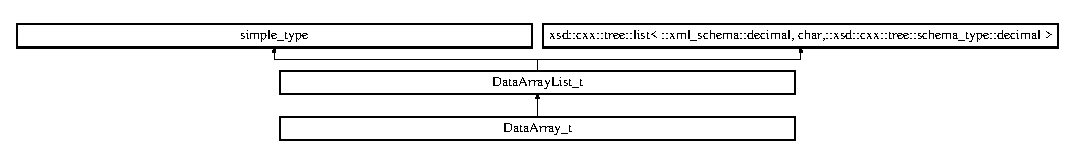
\includegraphics[height=1.660079cm]{classDataArrayList__t}
\end{center}
\end{figure}
\subsection*{Public Member Functions}
\begin{DoxyCompactItemize}
\item 
\hyperlink{classDataArrayList__t_a3ec10a5824450940e47a90c376fdb065}{Data\+Array\+List\+\_\+t} ()
\item 
\hyperlink{classDataArrayList__t_ad821001ed5f5f94f06712f5b0acab874}{Data\+Array\+List\+\_\+t} (size\+\_\+type n, const \+::\hyperlink{namespacexml__schema_a69bfaf24f63a8c18ebd8e21db6b343df}{xml\+\_\+schema\+::decimal} \&x)
\item 
{\footnotesize template$<$typename I $>$ }\\\hyperlink{classDataArrayList__t_a7b3c40bcc5d41bafc235a30ffa1a3b8f}{Data\+Array\+List\+\_\+t} (const I \&begin, const I \&end)
\item 
\hyperlink{classDataArrayList__t_ab596ca97e9666c979d1db13a4e032869}{Data\+Array\+List\+\_\+t} (const \+::xercesc\+::\+D\+O\+M\+Element \&e,\+::\hyperlink{namespacexml__schema_a0612287d030cb2732d31a45b258fdc87}{xml\+\_\+schema\+::flags} f=0,\+::\hyperlink{namespacexml__schema_ada9aa30dc722e93ee2ed7243085402a5}{xml\+\_\+schema\+::container} $\ast$c=0)
\item 
\hyperlink{classDataArrayList__t_a4cae1891a3ad2b9336b478fa436f4d3f}{Data\+Array\+List\+\_\+t} (const \+::xercesc\+::\+D\+O\+M\+Attr \&a,\+::\hyperlink{namespacexml__schema_a0612287d030cb2732d31a45b258fdc87}{xml\+\_\+schema\+::flags} f=0,\+::\hyperlink{namespacexml__schema_ada9aa30dc722e93ee2ed7243085402a5}{xml\+\_\+schema\+::container} $\ast$c=0)
\item 
\hyperlink{classDataArrayList__t_a360a3281299fcb02ad34ad0b2c2d15fd}{Data\+Array\+List\+\_\+t} (const \+::std\+::string \&s, const \+::xercesc\+::\+D\+O\+M\+Element $\ast$e,\+::\hyperlink{namespacexml__schema_a0612287d030cb2732d31a45b258fdc87}{xml\+\_\+schema\+::flags} f=0,\+::\hyperlink{namespacexml__schema_ada9aa30dc722e93ee2ed7243085402a5}{xml\+\_\+schema\+::container} $\ast$c=0)
\item 
\hyperlink{classDataArrayList__t_af44b66e9ba5c6f84a3a0cca1c0fc98dc}{Data\+Array\+List\+\_\+t} (const \hyperlink{classDataArrayList__t}{Data\+Array\+List\+\_\+t} \&x,\+::\hyperlink{namespacexml__schema_a0612287d030cb2732d31a45b258fdc87}{xml\+\_\+schema\+::flags} f=0,\+::\hyperlink{namespacexml__schema_ada9aa30dc722e93ee2ed7243085402a5}{xml\+\_\+schema\+::container} $\ast$c=0)
\item 
virtual \hyperlink{classDataArrayList__t}{Data\+Array\+List\+\_\+t} $\ast$ \hyperlink{classDataArrayList__t_acec29e88488ded1352c5b064827f5c38}{\+\_\+clone} (\+::\hyperlink{namespacexml__schema_a0612287d030cb2732d31a45b258fdc87}{xml\+\_\+schema\+::flags} f=0,\+::\hyperlink{namespacexml__schema_ada9aa30dc722e93ee2ed7243085402a5}{xml\+\_\+schema\+::container} $\ast$c=0) const 
\item 
virtual \hyperlink{classDataArrayList__t_aee3c16237122c72a9c163847232d830f}{$\sim$\+Data\+Array\+List\+\_\+t} ()
\end{DoxyCompactItemize}


\subsection{Constructor \& Destructor Documentation}
\index{Data\+Array\+List\+\_\+t@{Data\+Array\+List\+\_\+t}!Data\+Array\+List\+\_\+t@{Data\+Array\+List\+\_\+t}}
\index{Data\+Array\+List\+\_\+t@{Data\+Array\+List\+\_\+t}!Data\+Array\+List\+\_\+t@{Data\+Array\+List\+\_\+t}}
\subsubsection[{\texorpdfstring{Data\+Array\+List\+\_\+t()}{DataArrayList_t()}}]{\setlength{\rightskip}{0pt plus 5cm}Data\+Array\+List\+\_\+t\+::\+Data\+Array\+List\+\_\+t (
\begin{DoxyParamCaption}
{}
\end{DoxyParamCaption}
)}\hypertarget{classDataArrayList__t_a3ec10a5824450940e47a90c376fdb065}{}\label{classDataArrayList__t_a3ec10a5824450940e47a90c376fdb065}
\index{Data\+Array\+List\+\_\+t@{Data\+Array\+List\+\_\+t}!Data\+Array\+List\+\_\+t@{Data\+Array\+List\+\_\+t}}
\index{Data\+Array\+List\+\_\+t@{Data\+Array\+List\+\_\+t}!Data\+Array\+List\+\_\+t@{Data\+Array\+List\+\_\+t}}
\subsubsection[{\texorpdfstring{Data\+Array\+List\+\_\+t(size\+\_\+type n, const \+::xml\+\_\+schema\+::decimal \&x)}{DataArrayList_t(size_type n, const ::xml_schema::decimal &x)}}]{\setlength{\rightskip}{0pt plus 5cm}Data\+Array\+List\+\_\+t\+::\+Data\+Array\+List\+\_\+t (
\begin{DoxyParamCaption}
\item[{size\+\_\+type}]{n, }
\item[{const \+::{\bf xml\+\_\+schema\+::decimal} \&}]{x}
\end{DoxyParamCaption}
)}\hypertarget{classDataArrayList__t_ad821001ed5f5f94f06712f5b0acab874}{}\label{classDataArrayList__t_ad821001ed5f5f94f06712f5b0acab874}
\index{Data\+Array\+List\+\_\+t@{Data\+Array\+List\+\_\+t}!Data\+Array\+List\+\_\+t@{Data\+Array\+List\+\_\+t}}
\index{Data\+Array\+List\+\_\+t@{Data\+Array\+List\+\_\+t}!Data\+Array\+List\+\_\+t@{Data\+Array\+List\+\_\+t}}
\subsubsection[{\texorpdfstring{Data\+Array\+List\+\_\+t(const I \&begin, const I \&end)}{DataArrayList_t(const I &begin, const I &end)}}]{\setlength{\rightskip}{0pt plus 5cm}template$<$typename I $>$ Data\+Array\+List\+\_\+t\+::\+Data\+Array\+List\+\_\+t (
\begin{DoxyParamCaption}
\item[{const I \&}]{begin, }
\item[{const I \&}]{end}
\end{DoxyParamCaption}
)\hspace{0.3cm}{\ttfamily [inline]}}\hypertarget{classDataArrayList__t_a7b3c40bcc5d41bafc235a30ffa1a3b8f}{}\label{classDataArrayList__t_a7b3c40bcc5d41bafc235a30ffa1a3b8f}
\index{Data\+Array\+List\+\_\+t@{Data\+Array\+List\+\_\+t}!Data\+Array\+List\+\_\+t@{Data\+Array\+List\+\_\+t}}
\index{Data\+Array\+List\+\_\+t@{Data\+Array\+List\+\_\+t}!Data\+Array\+List\+\_\+t@{Data\+Array\+List\+\_\+t}}
\subsubsection[{\texorpdfstring{Data\+Array\+List\+\_\+t(const \+::xercesc\+::\+D\+O\+M\+Element \&e,\+::xml\+\_\+schema\+::flags f=0,\+::xml\+\_\+schema\+::container $\ast$c=0)}{DataArrayList_t(const ::xercesc::DOMElement &e,::xml_schema::flags f=0,::xml_schema::container *c=0)}}]{\setlength{\rightskip}{0pt plus 5cm}Data\+Array\+List\+\_\+t\+::\+Data\+Array\+List\+\_\+t (
\begin{DoxyParamCaption}
\item[{const \+::xercesc\+::\+D\+O\+M\+Element \&}]{e, }
\item[{\+::{\bf xml\+\_\+schema\+::flags}}]{f = {\ttfamily 0}, }
\item[{\+::{\bf xml\+\_\+schema\+::container} $\ast$}]{c = {\ttfamily 0}}
\end{DoxyParamCaption}
)}\hypertarget{classDataArrayList__t_ab596ca97e9666c979d1db13a4e032869}{}\label{classDataArrayList__t_ab596ca97e9666c979d1db13a4e032869}
\index{Data\+Array\+List\+\_\+t@{Data\+Array\+List\+\_\+t}!Data\+Array\+List\+\_\+t@{Data\+Array\+List\+\_\+t}}
\index{Data\+Array\+List\+\_\+t@{Data\+Array\+List\+\_\+t}!Data\+Array\+List\+\_\+t@{Data\+Array\+List\+\_\+t}}
\subsubsection[{\texorpdfstring{Data\+Array\+List\+\_\+t(const \+::xercesc\+::\+D\+O\+M\+Attr \&a,\+::xml\+\_\+schema\+::flags f=0,\+::xml\+\_\+schema\+::container $\ast$c=0)}{DataArrayList_t(const ::xercesc::DOMAttr &a,::xml_schema::flags f=0,::xml_schema::container *c=0)}}]{\setlength{\rightskip}{0pt plus 5cm}Data\+Array\+List\+\_\+t\+::\+Data\+Array\+List\+\_\+t (
\begin{DoxyParamCaption}
\item[{const \+::xercesc\+::\+D\+O\+M\+Attr \&}]{a, }
\item[{\+::{\bf xml\+\_\+schema\+::flags}}]{f = {\ttfamily 0}, }
\item[{\+::{\bf xml\+\_\+schema\+::container} $\ast$}]{c = {\ttfamily 0}}
\end{DoxyParamCaption}
)}\hypertarget{classDataArrayList__t_a4cae1891a3ad2b9336b478fa436f4d3f}{}\label{classDataArrayList__t_a4cae1891a3ad2b9336b478fa436f4d3f}
\index{Data\+Array\+List\+\_\+t@{Data\+Array\+List\+\_\+t}!Data\+Array\+List\+\_\+t@{Data\+Array\+List\+\_\+t}}
\index{Data\+Array\+List\+\_\+t@{Data\+Array\+List\+\_\+t}!Data\+Array\+List\+\_\+t@{Data\+Array\+List\+\_\+t}}
\subsubsection[{\texorpdfstring{Data\+Array\+List\+\_\+t(const \+::std\+::string \&s, const \+::xercesc\+::\+D\+O\+M\+Element $\ast$e,\+::xml\+\_\+schema\+::flags f=0,\+::xml\+\_\+schema\+::container $\ast$c=0)}{DataArrayList_t(const ::std::string &s, const ::xercesc::DOMElement *e,::xml_schema::flags f=0,::xml_schema::container *c=0)}}]{\setlength{\rightskip}{0pt plus 5cm}Data\+Array\+List\+\_\+t\+::\+Data\+Array\+List\+\_\+t (
\begin{DoxyParamCaption}
\item[{const \+::std\+::string \&}]{s, }
\item[{const \+::xercesc\+::\+D\+O\+M\+Element $\ast$}]{e, }
\item[{\+::{\bf xml\+\_\+schema\+::flags}}]{f = {\ttfamily 0}, }
\item[{\+::{\bf xml\+\_\+schema\+::container} $\ast$}]{c = {\ttfamily 0}}
\end{DoxyParamCaption}
)}\hypertarget{classDataArrayList__t_a360a3281299fcb02ad34ad0b2c2d15fd}{}\label{classDataArrayList__t_a360a3281299fcb02ad34ad0b2c2d15fd}
\index{Data\+Array\+List\+\_\+t@{Data\+Array\+List\+\_\+t}!Data\+Array\+List\+\_\+t@{Data\+Array\+List\+\_\+t}}
\index{Data\+Array\+List\+\_\+t@{Data\+Array\+List\+\_\+t}!Data\+Array\+List\+\_\+t@{Data\+Array\+List\+\_\+t}}
\subsubsection[{\texorpdfstring{Data\+Array\+List\+\_\+t(const Data\+Array\+List\+\_\+t \&x,\+::xml\+\_\+schema\+::flags f=0,\+::xml\+\_\+schema\+::container $\ast$c=0)}{DataArrayList_t(const DataArrayList_t &x,::xml_schema::flags f=0,::xml_schema::container *c=0)}}]{\setlength{\rightskip}{0pt plus 5cm}Data\+Array\+List\+\_\+t\+::\+Data\+Array\+List\+\_\+t (
\begin{DoxyParamCaption}
\item[{const {\bf Data\+Array\+List\+\_\+t} \&}]{x, }
\item[{\+::{\bf xml\+\_\+schema\+::flags}}]{f = {\ttfamily 0}, }
\item[{\+::{\bf xml\+\_\+schema\+::container} $\ast$}]{c = {\ttfamily 0}}
\end{DoxyParamCaption}
)}\hypertarget{classDataArrayList__t_af44b66e9ba5c6f84a3a0cca1c0fc98dc}{}\label{classDataArrayList__t_af44b66e9ba5c6f84a3a0cca1c0fc98dc}
\index{Data\+Array\+List\+\_\+t@{Data\+Array\+List\+\_\+t}!````~Data\+Array\+List\+\_\+t@{$\sim$\+Data\+Array\+List\+\_\+t}}
\index{````~Data\+Array\+List\+\_\+t@{$\sim$\+Data\+Array\+List\+\_\+t}!Data\+Array\+List\+\_\+t@{Data\+Array\+List\+\_\+t}}
\subsubsection[{\texorpdfstring{$\sim$\+Data\+Array\+List\+\_\+t()}{~DataArrayList_t()}}]{\setlength{\rightskip}{0pt plus 5cm}Data\+Array\+List\+\_\+t\+::$\sim$\+Data\+Array\+List\+\_\+t (
\begin{DoxyParamCaption}
{}
\end{DoxyParamCaption}
)\hspace{0.3cm}{\ttfamily [virtual]}}\hypertarget{classDataArrayList__t_aee3c16237122c72a9c163847232d830f}{}\label{classDataArrayList__t_aee3c16237122c72a9c163847232d830f}


\subsection{Member Function Documentation}
\index{Data\+Array\+List\+\_\+t@{Data\+Array\+List\+\_\+t}!\+\_\+clone@{\+\_\+clone}}
\index{\+\_\+clone@{\+\_\+clone}!Data\+Array\+List\+\_\+t@{Data\+Array\+List\+\_\+t}}
\subsubsection[{\texorpdfstring{\+\_\+clone(\+::xml\+\_\+schema\+::flags f=0,\+::xml\+\_\+schema\+::container $\ast$c=0) const }{_clone(::xml_schema::flags f=0,::xml_schema::container *c=0) const }}]{\setlength{\rightskip}{0pt plus 5cm}{\bf Data\+Array\+List\+\_\+t} $\ast$ Data\+Array\+List\+\_\+t\+::\+\_\+clone (
\begin{DoxyParamCaption}
\item[{\+::{\bf xml\+\_\+schema\+::flags}}]{f = {\ttfamily 0}, }
\item[{\+::{\bf xml\+\_\+schema\+::container} $\ast$}]{c = {\ttfamily 0}}
\end{DoxyParamCaption}
) const\hspace{0.3cm}{\ttfamily [virtual]}}\hypertarget{classDataArrayList__t_acec29e88488ded1352c5b064827f5c38}{}\label{classDataArrayList__t_acec29e88488ded1352c5b064827f5c38}


Reimplemented in \hyperlink{classDataArray__t_a0ba3569846912b9fcadbd942e914cce1}{Data\+Array\+\_\+t}.



The documentation for this class was generated from the following files\+:\begin{DoxyCompactItemize}
\item 
src/output\+Writer/\hyperlink{vtk-unstructured_8h}{vtk-\/unstructured.\+h}\item 
src/output\+Writer/\hyperlink{vtk-unstructured_8cpp}{vtk-\/unstructured.\+cpp}\end{DoxyCompactItemize}

\hypertarget{classFileReader}{}\section{File\+Reader Class Reference}
\label{classFileReader}\index{File\+Reader@{File\+Reader}}


{\ttfamily \#include $<$File\+Reader.\+h$>$}

\subsection*{Public Member Functions}
\begin{DoxyCompactItemize}
\item 
\hyperlink{classFileReader_a615dcb2443cad1f2ca123c7c0c334480}{File\+Reader} ()
\item 
virtual \hyperlink{classFileReader_a1382969e8f1468f3b04ad4b44ab39dee}{$\sim$\+File\+Reader} ()
\item 
void \hyperlink{classFileReader_a6392ce87a42739faa0ebd8bda06d5c2c}{read\+File} (\hyperlink{classParticleContainer}{Particle\+Container} $\ast$particles, const char $\ast$filename, double Rcutoff)
\end{DoxyCompactItemize}


\subsection{Constructor \& Destructor Documentation}
\index{File\+Reader@{File\+Reader}!File\+Reader@{File\+Reader}}
\index{File\+Reader@{File\+Reader}!File\+Reader@{File\+Reader}}
\subsubsection[{\texorpdfstring{File\+Reader()}{FileReader()}}]{\setlength{\rightskip}{0pt plus 5cm}File\+Reader\+::\+File\+Reader (
\begin{DoxyParamCaption}
{}
\end{DoxyParamCaption}
)}\hypertarget{classFileReader_a615dcb2443cad1f2ca123c7c0c334480}{}\label{classFileReader_a615dcb2443cad1f2ca123c7c0c334480}
\index{File\+Reader@{File\+Reader}!````~File\+Reader@{$\sim$\+File\+Reader}}
\index{````~File\+Reader@{$\sim$\+File\+Reader}!File\+Reader@{File\+Reader}}
\subsubsection[{\texorpdfstring{$\sim$\+File\+Reader()}{~FileReader()}}]{\setlength{\rightskip}{0pt plus 5cm}File\+Reader\+::$\sim$\+File\+Reader (
\begin{DoxyParamCaption}
{}
\end{DoxyParamCaption}
)\hspace{0.3cm}{\ttfamily [virtual]}}\hypertarget{classFileReader_a1382969e8f1468f3b04ad4b44ab39dee}{}\label{classFileReader_a1382969e8f1468f3b04ad4b44ab39dee}


\subsection{Member Function Documentation}
\index{File\+Reader@{File\+Reader}!read\+File@{read\+File}}
\index{read\+File@{read\+File}!File\+Reader@{File\+Reader}}
\subsubsection[{\texorpdfstring{read\+File(\+Particle\+Container $\ast$particles, const char $\ast$filename, double Rcutoff)}{readFile(ParticleContainer *particles, const char *filename, double Rcutoff)}}]{\setlength{\rightskip}{0pt plus 5cm}void File\+Reader\+::read\+File (
\begin{DoxyParamCaption}
\item[{{\bf Particle\+Container} $\ast$}]{particles, }
\item[{const char $\ast$}]{filename, }
\item[{double}]{Rcutoff}
\end{DoxyParamCaption}
)}\hypertarget{classFileReader_a6392ce87a42739faa0ebd8bda06d5c2c}{}\label{classFileReader_a6392ce87a42739faa0ebd8bda06d5c2c}
Fill a particle container with particles from a xml-\/file 
\begin{DoxyParams}{Parameters}
{\em particles} & the container to fill \\
\hline
{\em filename} & the path to the xml-\/file containing information to generate the particles \\
\hline
{\em Rcutoff} & distance to set the truncation distance of the L\+J-\/calculation \\
\hline
\end{DoxyParams}


The documentation for this class was generated from the following files\+:\begin{DoxyCompactItemize}
\item 
src/input/\hyperlink{FileReader_8h}{File\+Reader.\+h}\item 
src/input/\hyperlink{FileReader_8cpp}{File\+Reader.\+cpp}\end{DoxyCompactItemize}

\hypertarget{classinput__t}{}\section{input\+\_\+t Class Reference}
\label{classinput__t}\index{input\+\_\+t@{input\+\_\+t}}


{\ttfamily \#include $<$particle\+\_\+input.\+h$>$}

Inheritance diagram for input\+\_\+t\+:\begin{figure}[H]
\begin{center}
\leavevmode
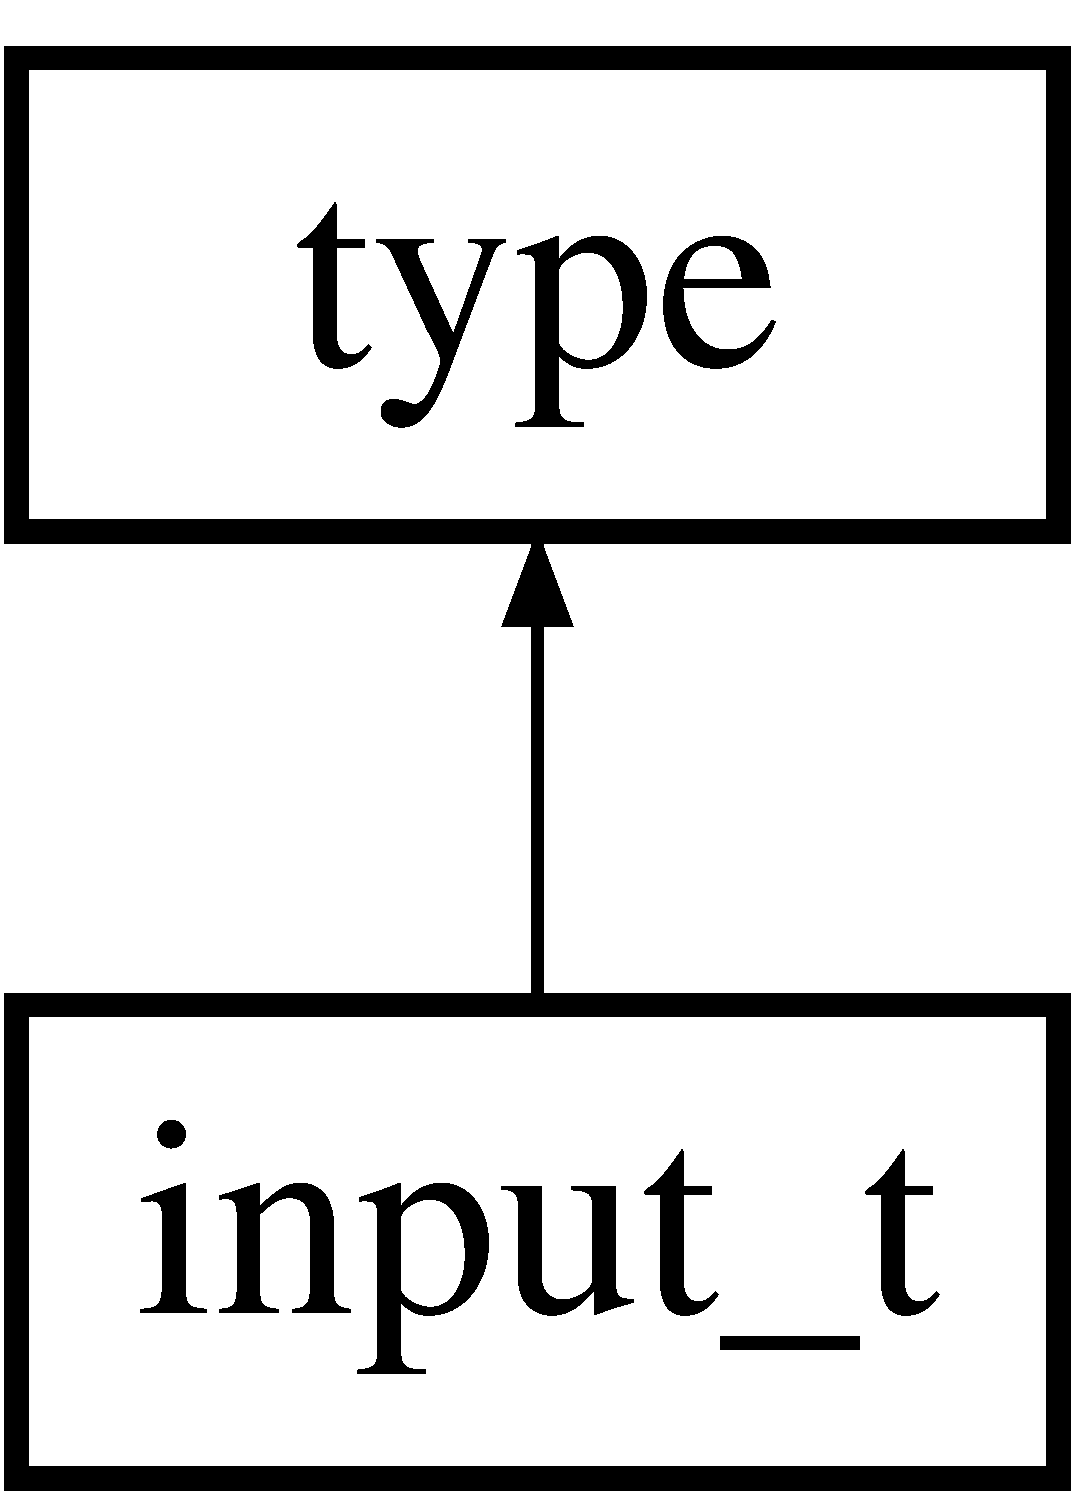
\includegraphics[height=2.000000cm]{classinput__t}
\end{center}
\end{figure}
\subsection*{Public Types}
\begin{DoxyCompactItemize}
\item 
typedef \+::\hyperlink{classparticletype__t}{particletype\+\_\+t} \hyperlink{classinput__t_a516c75c9426ee0026078ebe9ee6f50ea}{types\+\_\+input\+\_\+type}
\item 
typedef \+::xsd\+::cxx\+::tree\+::sequence$<$ \hyperlink{classinput__t_a516c75c9426ee0026078ebe9ee6f50ea}{types\+\_\+input\+\_\+type} $>$ \hyperlink{classinput__t_a48f5b9f6b00c9d3749caf0e3a0eac5a7}{types\+\_\+input\+\_\+sequence}
\item 
typedef types\+\_\+input\+\_\+sequence\+::iterator \hyperlink{classinput__t_a830eb55890cdf67c70880536db78be04}{types\+\_\+input\+\_\+iterator}
\item 
typedef types\+\_\+input\+\_\+sequence\+::const\+\_\+iterator \hyperlink{classinput__t_a7fddef7619e8c4dd76b1c6448c42bfc0}{types\+\_\+input\+\_\+const\+\_\+iterator}
\item 
typedef \+::xsd\+::cxx\+::tree\+::traits$<$ \hyperlink{classinput__t_a516c75c9426ee0026078ebe9ee6f50ea}{types\+\_\+input\+\_\+type}, char $>$ \hyperlink{classinput__t_a7ab3dea1712373b005d910f827cd9753}{types\+\_\+input\+\_\+traits}
\item 
typedef \+::\hyperlink{classsingle__t}{single\+\_\+t} \hyperlink{classinput__t_af24fd90c4a0fa092c577776efca1c750}{single\+\_\+input\+\_\+type}
\item 
typedef \+::xsd\+::cxx\+::tree\+::sequence$<$ \hyperlink{classinput__t_af24fd90c4a0fa092c577776efca1c750}{single\+\_\+input\+\_\+type} $>$ \hyperlink{classinput__t_a1296075494d97da854dc2be8b1022061}{single\+\_\+input\+\_\+sequence}
\item 
typedef single\+\_\+input\+\_\+sequence\+::iterator \hyperlink{classinput__t_a001a8bb6bb06d71002249f491bc628fa}{single\+\_\+input\+\_\+iterator}
\item 
typedef single\+\_\+input\+\_\+sequence\+::const\+\_\+iterator \hyperlink{classinput__t_ac6c5ac99d56764bfdf61d747cd2c2074}{single\+\_\+input\+\_\+const\+\_\+iterator}
\item 
typedef \+::xsd\+::cxx\+::tree\+::traits$<$ \hyperlink{classinput__t_af24fd90c4a0fa092c577776efca1c750}{single\+\_\+input\+\_\+type}, char $>$ \hyperlink{classinput__t_aa3a5fc9d04df805785a23a89248fa924}{single\+\_\+input\+\_\+traits}
\item 
typedef \+::\hyperlink{classcuboid__t}{cuboid\+\_\+t} \hyperlink{classinput__t_ab3172aa59d0cc9b2d4c5380d9cec72c3}{cuboid\+\_\+input\+\_\+type}
\item 
typedef \+::xsd\+::cxx\+::tree\+::sequence$<$ \hyperlink{classinput__t_ab3172aa59d0cc9b2d4c5380d9cec72c3}{cuboid\+\_\+input\+\_\+type} $>$ \hyperlink{classinput__t_a5aef33216e01e60c197cea604a519ab4}{cuboid\+\_\+input\+\_\+sequence}
\item 
typedef cuboid\+\_\+input\+\_\+sequence\+::iterator \hyperlink{classinput__t_aa4ecd719f9c1e557f73c163c723259f2}{cuboid\+\_\+input\+\_\+iterator}
\item 
typedef cuboid\+\_\+input\+\_\+sequence\+::const\+\_\+iterator \hyperlink{classinput__t_aab1823936b590269cb0f4de2f0a0a4fa}{cuboid\+\_\+input\+\_\+const\+\_\+iterator}
\item 
typedef \+::xsd\+::cxx\+::tree\+::traits$<$ \hyperlink{classinput__t_ab3172aa59d0cc9b2d4c5380d9cec72c3}{cuboid\+\_\+input\+\_\+type}, char $>$ \hyperlink{classinput__t_a6d747b3e200566247dcf36dd80109730}{cuboid\+\_\+input\+\_\+traits}
\item 
typedef \+::\hyperlink{classmembrane__t}{membrane\+\_\+t} \hyperlink{classinput__t_aa72abd8e01641f20e6fdb3d5d0bf99ca}{membrane\+\_\+input\+\_\+type}
\item 
typedef \+::xsd\+::cxx\+::tree\+::sequence$<$ \hyperlink{classinput__t_aa72abd8e01641f20e6fdb3d5d0bf99ca}{membrane\+\_\+input\+\_\+type} $>$ \hyperlink{classinput__t_a455e36bc8b009abdbd13c6d167864cfe}{membrane\+\_\+input\+\_\+sequence}
\item 
typedef membrane\+\_\+input\+\_\+sequence\+::iterator \hyperlink{classinput__t_a2a9ad5a60f532541071c8432e3f3333b}{membrane\+\_\+input\+\_\+iterator}
\item 
typedef membrane\+\_\+input\+\_\+sequence\+::const\+\_\+iterator \hyperlink{classinput__t_ad9f1a19dff09cac44dc94fd97b3ab778}{membrane\+\_\+input\+\_\+const\+\_\+iterator}
\item 
typedef \+::xsd\+::cxx\+::tree\+::traits$<$ \hyperlink{classinput__t_aa72abd8e01641f20e6fdb3d5d0bf99ca}{membrane\+\_\+input\+\_\+type}, char $>$ \hyperlink{classinput__t_a7d8560c1644f93d6491d5aad368aeddb}{membrane\+\_\+input\+\_\+traits}
\item 
typedef \+::\hyperlink{classsphere__t}{sphere\+\_\+t} \hyperlink{classinput__t_a75628386280268669a4cc94066bd8547}{sphere\+\_\+input\+\_\+type}
\item 
typedef \+::xsd\+::cxx\+::tree\+::sequence$<$ \hyperlink{classinput__t_a75628386280268669a4cc94066bd8547}{sphere\+\_\+input\+\_\+type} $>$ \hyperlink{classinput__t_aa968afe5c55f7cc3031e6196adddcae5}{sphere\+\_\+input\+\_\+sequence}
\item 
typedef sphere\+\_\+input\+\_\+sequence\+::iterator \hyperlink{classinput__t_ab8ba0d1f12d650cf8f5db6b8262baa0e}{sphere\+\_\+input\+\_\+iterator}
\item 
typedef sphere\+\_\+input\+\_\+sequence\+::const\+\_\+iterator \hyperlink{classinput__t_aa281fd31856422d1cb3934608b8e0185}{sphere\+\_\+input\+\_\+const\+\_\+iterator}
\item 
typedef \+::xsd\+::cxx\+::tree\+::traits$<$ \hyperlink{classinput__t_a75628386280268669a4cc94066bd8547}{sphere\+\_\+input\+\_\+type}, char $>$ \hyperlink{classinput__t_afb3a266016b34553b5f045eaddf78031}{sphere\+\_\+input\+\_\+traits}
\end{DoxyCompactItemize}
\subsection*{Public Member Functions}
\begin{DoxyCompactItemize}
\item 
const \hyperlink{classinput__t_a48f5b9f6b00c9d3749caf0e3a0eac5a7}{types\+\_\+input\+\_\+sequence} \& \hyperlink{classinput__t_aad81ec0c8587d9ed3c0390cc9ba75bb0}{types\+\_\+input} () const 
\item 
\hyperlink{classinput__t_a48f5b9f6b00c9d3749caf0e3a0eac5a7}{types\+\_\+input\+\_\+sequence} \& \hyperlink{classinput__t_a70e55b1ecc015b3e00101928dfbe5464}{types\+\_\+input} ()
\item 
void \hyperlink{classinput__t_a8a371e78d74ad9f67271745117ad478a}{types\+\_\+input} (const \hyperlink{classinput__t_a48f5b9f6b00c9d3749caf0e3a0eac5a7}{types\+\_\+input\+\_\+sequence} \&s)
\item 
const \hyperlink{classinput__t_a1296075494d97da854dc2be8b1022061}{single\+\_\+input\+\_\+sequence} \& \hyperlink{classinput__t_a23df17feba2a762f381167fbd900e3e2}{single\+\_\+input} () const 
\item 
\hyperlink{classinput__t_a1296075494d97da854dc2be8b1022061}{single\+\_\+input\+\_\+sequence} \& \hyperlink{classinput__t_abf4899015034fd15a532960d94af0388}{single\+\_\+input} ()
\item 
void \hyperlink{classinput__t_a76b473ba9a3a25f8d2c7ed2c02489c2d}{single\+\_\+input} (const \hyperlink{classinput__t_a1296075494d97da854dc2be8b1022061}{single\+\_\+input\+\_\+sequence} \&s)
\item 
const \hyperlink{classinput__t_a5aef33216e01e60c197cea604a519ab4}{cuboid\+\_\+input\+\_\+sequence} \& \hyperlink{classinput__t_a59b8093194c770faf0efcf86eb7a7383}{cuboid\+\_\+input} () const 
\item 
\hyperlink{classinput__t_a5aef33216e01e60c197cea604a519ab4}{cuboid\+\_\+input\+\_\+sequence} \& \hyperlink{classinput__t_af66b8c90f49b958d6e5f2b236abad9b2}{cuboid\+\_\+input} ()
\item 
void \hyperlink{classinput__t_a4d1a25864dfaf5d4ab006425538b1125}{cuboid\+\_\+input} (const \hyperlink{classinput__t_a5aef33216e01e60c197cea604a519ab4}{cuboid\+\_\+input\+\_\+sequence} \&s)
\item 
const \hyperlink{classinput__t_a455e36bc8b009abdbd13c6d167864cfe}{membrane\+\_\+input\+\_\+sequence} \& \hyperlink{classinput__t_adba6d36e90b80fe27862a3f7fc5fbf2a}{membrane\+\_\+input} () const 
\item 
\hyperlink{classinput__t_a455e36bc8b009abdbd13c6d167864cfe}{membrane\+\_\+input\+\_\+sequence} \& \hyperlink{classinput__t_a921b08f23c98a6c2aa7f4fb0c707a3ea}{membrane\+\_\+input} ()
\item 
void \hyperlink{classinput__t_a790aa48e13cbc7b014a70109a5942903}{membrane\+\_\+input} (const \hyperlink{classinput__t_a455e36bc8b009abdbd13c6d167864cfe}{membrane\+\_\+input\+\_\+sequence} \&s)
\item 
const \hyperlink{classinput__t_aa968afe5c55f7cc3031e6196adddcae5}{sphere\+\_\+input\+\_\+sequence} \& \hyperlink{classinput__t_abb6b015f0faa92bff850d921d4aad2b7}{sphere\+\_\+input} () const 
\item 
\hyperlink{classinput__t_aa968afe5c55f7cc3031e6196adddcae5}{sphere\+\_\+input\+\_\+sequence} \& \hyperlink{classinput__t_a3173f5cec229bff952ac6d965135d0ca}{sphere\+\_\+input} ()
\item 
void \hyperlink{classinput__t_acf44523ff6b17315300e30fbebe9f6db}{sphere\+\_\+input} (const \hyperlink{classinput__t_aa968afe5c55f7cc3031e6196adddcae5}{sphere\+\_\+input\+\_\+sequence} \&s)
\item 
\hyperlink{classinput__t_acd30ace524c19489ac1076e29e29c4cf}{input\+\_\+t} ()
\item 
\hyperlink{classinput__t_ad5e6bb4ad3034e6072766d292a9b2f06}{input\+\_\+t} (const \+::xercesc\+::\+D\+O\+M\+Element \&e,\+::\hyperlink{namespacexml__schema_a0612287d030cb2732d31a45b258fdc87}{xml\+\_\+schema\+::flags} f=0,\+::\hyperlink{namespacexml__schema_ada9aa30dc722e93ee2ed7243085402a5}{xml\+\_\+schema\+::container} $\ast$c=0)
\item 
\hyperlink{classinput__t_aa61c09ee6e6c8849e08296ea0ce9cdf9}{input\+\_\+t} (const \hyperlink{classinput__t}{input\+\_\+t} \&x,\+::\hyperlink{namespacexml__schema_a0612287d030cb2732d31a45b258fdc87}{xml\+\_\+schema\+::flags} f=0,\+::\hyperlink{namespacexml__schema_ada9aa30dc722e93ee2ed7243085402a5}{xml\+\_\+schema\+::container} $\ast$c=0)
\item 
virtual \hyperlink{classinput__t}{input\+\_\+t} $\ast$ \hyperlink{classinput__t_a5113f4bf339b6e9f325fa1c0dc2a03de}{\+\_\+clone} (\+::\hyperlink{namespacexml__schema_a0612287d030cb2732d31a45b258fdc87}{xml\+\_\+schema\+::flags} f=0,\+::\hyperlink{namespacexml__schema_ada9aa30dc722e93ee2ed7243085402a5}{xml\+\_\+schema\+::container} $\ast$c=0) const 
\item 
\hyperlink{classinput__t}{input\+\_\+t} \& \hyperlink{classinput__t_ac0f3874f508379a49375e681699ffdc2}{operator=} (const \hyperlink{classinput__t}{input\+\_\+t} \&x)
\item 
virtual \hyperlink{classinput__t_adec69a9fb0ede4506dda7414275639c2}{$\sim$input\+\_\+t} ()
\end{DoxyCompactItemize}
\subsection*{Protected Member Functions}
\begin{DoxyCompactItemize}
\item 
void \hyperlink{classinput__t_af3861aa840c8d80dbbde88fae9b3db72}{parse} (\+::xsd\+::cxx\+::xml\+::dom\+::parser$<$ char $>$ \&,\+::\hyperlink{namespacexml__schema_a0612287d030cb2732d31a45b258fdc87}{xml\+\_\+schema\+::flags})
\end{DoxyCompactItemize}
\subsection*{Protected Attributes}
\begin{DoxyCompactItemize}
\item 
\hyperlink{classinput__t_a48f5b9f6b00c9d3749caf0e3a0eac5a7}{types\+\_\+input\+\_\+sequence} \hyperlink{classinput__t_af064e28d005941bce91337b136403cce}{types\+\_\+input\+\_\+}
\item 
\hyperlink{classinput__t_a1296075494d97da854dc2be8b1022061}{single\+\_\+input\+\_\+sequence} \hyperlink{classinput__t_a1f8f19b740102f74acb4dea4733350e4}{single\+\_\+input\+\_\+}
\item 
\hyperlink{classinput__t_a5aef33216e01e60c197cea604a519ab4}{cuboid\+\_\+input\+\_\+sequence} \hyperlink{classinput__t_af00e51fceddd64f134b3e7cd8707d692}{cuboid\+\_\+input\+\_\+}
\item 
\hyperlink{classinput__t_a455e36bc8b009abdbd13c6d167864cfe}{membrane\+\_\+input\+\_\+sequence} \hyperlink{classinput__t_a58ff5d3539fbe50257614d106dbf9dc4}{membrane\+\_\+input\+\_\+}
\item 
\hyperlink{classinput__t_aa968afe5c55f7cc3031e6196adddcae5}{sphere\+\_\+input\+\_\+sequence} \hyperlink{classinput__t_af9cafaeb8d3c98067e4a27edf2c2339e}{sphere\+\_\+input\+\_\+}
\end{DoxyCompactItemize}


\subsection{Member Typedef Documentation}
\index{input\+\_\+t@{input\+\_\+t}!cuboid\+\_\+input\+\_\+const\+\_\+iterator@{cuboid\+\_\+input\+\_\+const\+\_\+iterator}}
\index{cuboid\+\_\+input\+\_\+const\+\_\+iterator@{cuboid\+\_\+input\+\_\+const\+\_\+iterator}!input\+\_\+t@{input\+\_\+t}}
\subsubsection[{\texorpdfstring{cuboid\+\_\+input\+\_\+const\+\_\+iterator}{cuboid_input_const_iterator}}]{\setlength{\rightskip}{0pt plus 5cm}typedef cuboid\+\_\+input\+\_\+sequence\+::const\+\_\+iterator {\bf input\+\_\+t\+::cuboid\+\_\+input\+\_\+const\+\_\+iterator}}\hypertarget{classinput__t_aab1823936b590269cb0f4de2f0a0a4fa}{}\label{classinput__t_aab1823936b590269cb0f4de2f0a0a4fa}
\index{input\+\_\+t@{input\+\_\+t}!cuboid\+\_\+input\+\_\+iterator@{cuboid\+\_\+input\+\_\+iterator}}
\index{cuboid\+\_\+input\+\_\+iterator@{cuboid\+\_\+input\+\_\+iterator}!input\+\_\+t@{input\+\_\+t}}
\subsubsection[{\texorpdfstring{cuboid\+\_\+input\+\_\+iterator}{cuboid_input_iterator}}]{\setlength{\rightskip}{0pt plus 5cm}typedef cuboid\+\_\+input\+\_\+sequence\+::iterator {\bf input\+\_\+t\+::cuboid\+\_\+input\+\_\+iterator}}\hypertarget{classinput__t_aa4ecd719f9c1e557f73c163c723259f2}{}\label{classinput__t_aa4ecd719f9c1e557f73c163c723259f2}
\index{input\+\_\+t@{input\+\_\+t}!cuboid\+\_\+input\+\_\+sequence@{cuboid\+\_\+input\+\_\+sequence}}
\index{cuboid\+\_\+input\+\_\+sequence@{cuboid\+\_\+input\+\_\+sequence}!input\+\_\+t@{input\+\_\+t}}
\subsubsection[{\texorpdfstring{cuboid\+\_\+input\+\_\+sequence}{cuboid_input_sequence}}]{\setlength{\rightskip}{0pt plus 5cm}typedef \+::xsd\+::cxx\+::tree\+::sequence$<$ {\bf cuboid\+\_\+input\+\_\+type} $>$ {\bf input\+\_\+t\+::cuboid\+\_\+input\+\_\+sequence}}\hypertarget{classinput__t_a5aef33216e01e60c197cea604a519ab4}{}\label{classinput__t_a5aef33216e01e60c197cea604a519ab4}
\index{input\+\_\+t@{input\+\_\+t}!cuboid\+\_\+input\+\_\+traits@{cuboid\+\_\+input\+\_\+traits}}
\index{cuboid\+\_\+input\+\_\+traits@{cuboid\+\_\+input\+\_\+traits}!input\+\_\+t@{input\+\_\+t}}
\subsubsection[{\texorpdfstring{cuboid\+\_\+input\+\_\+traits}{cuboid_input_traits}}]{\setlength{\rightskip}{0pt plus 5cm}typedef \+::xsd\+::cxx\+::tree\+::traits$<$ {\bf cuboid\+\_\+input\+\_\+type}, char $>$ {\bf input\+\_\+t\+::cuboid\+\_\+input\+\_\+traits}}\hypertarget{classinput__t_a6d747b3e200566247dcf36dd80109730}{}\label{classinput__t_a6d747b3e200566247dcf36dd80109730}
\index{input\+\_\+t@{input\+\_\+t}!cuboid\+\_\+input\+\_\+type@{cuboid\+\_\+input\+\_\+type}}
\index{cuboid\+\_\+input\+\_\+type@{cuboid\+\_\+input\+\_\+type}!input\+\_\+t@{input\+\_\+t}}
\subsubsection[{\texorpdfstring{cuboid\+\_\+input\+\_\+type}{cuboid_input_type}}]{\setlength{\rightskip}{0pt plus 5cm}typedef \+::{\bf cuboid\+\_\+t} {\bf input\+\_\+t\+::cuboid\+\_\+input\+\_\+type}}\hypertarget{classinput__t_ab3172aa59d0cc9b2d4c5380d9cec72c3}{}\label{classinput__t_ab3172aa59d0cc9b2d4c5380d9cec72c3}
\index{input\+\_\+t@{input\+\_\+t}!membrane\+\_\+input\+\_\+const\+\_\+iterator@{membrane\+\_\+input\+\_\+const\+\_\+iterator}}
\index{membrane\+\_\+input\+\_\+const\+\_\+iterator@{membrane\+\_\+input\+\_\+const\+\_\+iterator}!input\+\_\+t@{input\+\_\+t}}
\subsubsection[{\texorpdfstring{membrane\+\_\+input\+\_\+const\+\_\+iterator}{membrane_input_const_iterator}}]{\setlength{\rightskip}{0pt plus 5cm}typedef membrane\+\_\+input\+\_\+sequence\+::const\+\_\+iterator {\bf input\+\_\+t\+::membrane\+\_\+input\+\_\+const\+\_\+iterator}}\hypertarget{classinput__t_ad9f1a19dff09cac44dc94fd97b3ab778}{}\label{classinput__t_ad9f1a19dff09cac44dc94fd97b3ab778}
\index{input\+\_\+t@{input\+\_\+t}!membrane\+\_\+input\+\_\+iterator@{membrane\+\_\+input\+\_\+iterator}}
\index{membrane\+\_\+input\+\_\+iterator@{membrane\+\_\+input\+\_\+iterator}!input\+\_\+t@{input\+\_\+t}}
\subsubsection[{\texorpdfstring{membrane\+\_\+input\+\_\+iterator}{membrane_input_iterator}}]{\setlength{\rightskip}{0pt plus 5cm}typedef membrane\+\_\+input\+\_\+sequence\+::iterator {\bf input\+\_\+t\+::membrane\+\_\+input\+\_\+iterator}}\hypertarget{classinput__t_a2a9ad5a60f532541071c8432e3f3333b}{}\label{classinput__t_a2a9ad5a60f532541071c8432e3f3333b}
\index{input\+\_\+t@{input\+\_\+t}!membrane\+\_\+input\+\_\+sequence@{membrane\+\_\+input\+\_\+sequence}}
\index{membrane\+\_\+input\+\_\+sequence@{membrane\+\_\+input\+\_\+sequence}!input\+\_\+t@{input\+\_\+t}}
\subsubsection[{\texorpdfstring{membrane\+\_\+input\+\_\+sequence}{membrane_input_sequence}}]{\setlength{\rightskip}{0pt plus 5cm}typedef \+::xsd\+::cxx\+::tree\+::sequence$<$ {\bf membrane\+\_\+input\+\_\+type} $>$ {\bf input\+\_\+t\+::membrane\+\_\+input\+\_\+sequence}}\hypertarget{classinput__t_a455e36bc8b009abdbd13c6d167864cfe}{}\label{classinput__t_a455e36bc8b009abdbd13c6d167864cfe}
\index{input\+\_\+t@{input\+\_\+t}!membrane\+\_\+input\+\_\+traits@{membrane\+\_\+input\+\_\+traits}}
\index{membrane\+\_\+input\+\_\+traits@{membrane\+\_\+input\+\_\+traits}!input\+\_\+t@{input\+\_\+t}}
\subsubsection[{\texorpdfstring{membrane\+\_\+input\+\_\+traits}{membrane_input_traits}}]{\setlength{\rightskip}{0pt plus 5cm}typedef \+::xsd\+::cxx\+::tree\+::traits$<$ {\bf membrane\+\_\+input\+\_\+type}, char $>$ {\bf input\+\_\+t\+::membrane\+\_\+input\+\_\+traits}}\hypertarget{classinput__t_a7d8560c1644f93d6491d5aad368aeddb}{}\label{classinput__t_a7d8560c1644f93d6491d5aad368aeddb}
\index{input\+\_\+t@{input\+\_\+t}!membrane\+\_\+input\+\_\+type@{membrane\+\_\+input\+\_\+type}}
\index{membrane\+\_\+input\+\_\+type@{membrane\+\_\+input\+\_\+type}!input\+\_\+t@{input\+\_\+t}}
\subsubsection[{\texorpdfstring{membrane\+\_\+input\+\_\+type}{membrane_input_type}}]{\setlength{\rightskip}{0pt plus 5cm}typedef \+::{\bf membrane\+\_\+t} {\bf input\+\_\+t\+::membrane\+\_\+input\+\_\+type}}\hypertarget{classinput__t_aa72abd8e01641f20e6fdb3d5d0bf99ca}{}\label{classinput__t_aa72abd8e01641f20e6fdb3d5d0bf99ca}
\index{input\+\_\+t@{input\+\_\+t}!single\+\_\+input\+\_\+const\+\_\+iterator@{single\+\_\+input\+\_\+const\+\_\+iterator}}
\index{single\+\_\+input\+\_\+const\+\_\+iterator@{single\+\_\+input\+\_\+const\+\_\+iterator}!input\+\_\+t@{input\+\_\+t}}
\subsubsection[{\texorpdfstring{single\+\_\+input\+\_\+const\+\_\+iterator}{single_input_const_iterator}}]{\setlength{\rightskip}{0pt plus 5cm}typedef single\+\_\+input\+\_\+sequence\+::const\+\_\+iterator {\bf input\+\_\+t\+::single\+\_\+input\+\_\+const\+\_\+iterator}}\hypertarget{classinput__t_ac6c5ac99d56764bfdf61d747cd2c2074}{}\label{classinput__t_ac6c5ac99d56764bfdf61d747cd2c2074}
\index{input\+\_\+t@{input\+\_\+t}!single\+\_\+input\+\_\+iterator@{single\+\_\+input\+\_\+iterator}}
\index{single\+\_\+input\+\_\+iterator@{single\+\_\+input\+\_\+iterator}!input\+\_\+t@{input\+\_\+t}}
\subsubsection[{\texorpdfstring{single\+\_\+input\+\_\+iterator}{single_input_iterator}}]{\setlength{\rightskip}{0pt plus 5cm}typedef single\+\_\+input\+\_\+sequence\+::iterator {\bf input\+\_\+t\+::single\+\_\+input\+\_\+iterator}}\hypertarget{classinput__t_a001a8bb6bb06d71002249f491bc628fa}{}\label{classinput__t_a001a8bb6bb06d71002249f491bc628fa}
\index{input\+\_\+t@{input\+\_\+t}!single\+\_\+input\+\_\+sequence@{single\+\_\+input\+\_\+sequence}}
\index{single\+\_\+input\+\_\+sequence@{single\+\_\+input\+\_\+sequence}!input\+\_\+t@{input\+\_\+t}}
\subsubsection[{\texorpdfstring{single\+\_\+input\+\_\+sequence}{single_input_sequence}}]{\setlength{\rightskip}{0pt plus 5cm}typedef \+::xsd\+::cxx\+::tree\+::sequence$<$ {\bf single\+\_\+input\+\_\+type} $>$ {\bf input\+\_\+t\+::single\+\_\+input\+\_\+sequence}}\hypertarget{classinput__t_a1296075494d97da854dc2be8b1022061}{}\label{classinput__t_a1296075494d97da854dc2be8b1022061}
\index{input\+\_\+t@{input\+\_\+t}!single\+\_\+input\+\_\+traits@{single\+\_\+input\+\_\+traits}}
\index{single\+\_\+input\+\_\+traits@{single\+\_\+input\+\_\+traits}!input\+\_\+t@{input\+\_\+t}}
\subsubsection[{\texorpdfstring{single\+\_\+input\+\_\+traits}{single_input_traits}}]{\setlength{\rightskip}{0pt plus 5cm}typedef \+::xsd\+::cxx\+::tree\+::traits$<$ {\bf single\+\_\+input\+\_\+type}, char $>$ {\bf input\+\_\+t\+::single\+\_\+input\+\_\+traits}}\hypertarget{classinput__t_aa3a5fc9d04df805785a23a89248fa924}{}\label{classinput__t_aa3a5fc9d04df805785a23a89248fa924}
\index{input\+\_\+t@{input\+\_\+t}!single\+\_\+input\+\_\+type@{single\+\_\+input\+\_\+type}}
\index{single\+\_\+input\+\_\+type@{single\+\_\+input\+\_\+type}!input\+\_\+t@{input\+\_\+t}}
\subsubsection[{\texorpdfstring{single\+\_\+input\+\_\+type}{single_input_type}}]{\setlength{\rightskip}{0pt plus 5cm}typedef \+::{\bf single\+\_\+t} {\bf input\+\_\+t\+::single\+\_\+input\+\_\+type}}\hypertarget{classinput__t_af24fd90c4a0fa092c577776efca1c750}{}\label{classinput__t_af24fd90c4a0fa092c577776efca1c750}
\index{input\+\_\+t@{input\+\_\+t}!sphere\+\_\+input\+\_\+const\+\_\+iterator@{sphere\+\_\+input\+\_\+const\+\_\+iterator}}
\index{sphere\+\_\+input\+\_\+const\+\_\+iterator@{sphere\+\_\+input\+\_\+const\+\_\+iterator}!input\+\_\+t@{input\+\_\+t}}
\subsubsection[{\texorpdfstring{sphere\+\_\+input\+\_\+const\+\_\+iterator}{sphere_input_const_iterator}}]{\setlength{\rightskip}{0pt plus 5cm}typedef sphere\+\_\+input\+\_\+sequence\+::const\+\_\+iterator {\bf input\+\_\+t\+::sphere\+\_\+input\+\_\+const\+\_\+iterator}}\hypertarget{classinput__t_aa281fd31856422d1cb3934608b8e0185}{}\label{classinput__t_aa281fd31856422d1cb3934608b8e0185}
\index{input\+\_\+t@{input\+\_\+t}!sphere\+\_\+input\+\_\+iterator@{sphere\+\_\+input\+\_\+iterator}}
\index{sphere\+\_\+input\+\_\+iterator@{sphere\+\_\+input\+\_\+iterator}!input\+\_\+t@{input\+\_\+t}}
\subsubsection[{\texorpdfstring{sphere\+\_\+input\+\_\+iterator}{sphere_input_iterator}}]{\setlength{\rightskip}{0pt plus 5cm}typedef sphere\+\_\+input\+\_\+sequence\+::iterator {\bf input\+\_\+t\+::sphere\+\_\+input\+\_\+iterator}}\hypertarget{classinput__t_ab8ba0d1f12d650cf8f5db6b8262baa0e}{}\label{classinput__t_ab8ba0d1f12d650cf8f5db6b8262baa0e}
\index{input\+\_\+t@{input\+\_\+t}!sphere\+\_\+input\+\_\+sequence@{sphere\+\_\+input\+\_\+sequence}}
\index{sphere\+\_\+input\+\_\+sequence@{sphere\+\_\+input\+\_\+sequence}!input\+\_\+t@{input\+\_\+t}}
\subsubsection[{\texorpdfstring{sphere\+\_\+input\+\_\+sequence}{sphere_input_sequence}}]{\setlength{\rightskip}{0pt plus 5cm}typedef \+::xsd\+::cxx\+::tree\+::sequence$<$ {\bf sphere\+\_\+input\+\_\+type} $>$ {\bf input\+\_\+t\+::sphere\+\_\+input\+\_\+sequence}}\hypertarget{classinput__t_aa968afe5c55f7cc3031e6196adddcae5}{}\label{classinput__t_aa968afe5c55f7cc3031e6196adddcae5}
\index{input\+\_\+t@{input\+\_\+t}!sphere\+\_\+input\+\_\+traits@{sphere\+\_\+input\+\_\+traits}}
\index{sphere\+\_\+input\+\_\+traits@{sphere\+\_\+input\+\_\+traits}!input\+\_\+t@{input\+\_\+t}}
\subsubsection[{\texorpdfstring{sphere\+\_\+input\+\_\+traits}{sphere_input_traits}}]{\setlength{\rightskip}{0pt plus 5cm}typedef \+::xsd\+::cxx\+::tree\+::traits$<$ {\bf sphere\+\_\+input\+\_\+type}, char $>$ {\bf input\+\_\+t\+::sphere\+\_\+input\+\_\+traits}}\hypertarget{classinput__t_afb3a266016b34553b5f045eaddf78031}{}\label{classinput__t_afb3a266016b34553b5f045eaddf78031}
\index{input\+\_\+t@{input\+\_\+t}!sphere\+\_\+input\+\_\+type@{sphere\+\_\+input\+\_\+type}}
\index{sphere\+\_\+input\+\_\+type@{sphere\+\_\+input\+\_\+type}!input\+\_\+t@{input\+\_\+t}}
\subsubsection[{\texorpdfstring{sphere\+\_\+input\+\_\+type}{sphere_input_type}}]{\setlength{\rightskip}{0pt plus 5cm}typedef \+::{\bf sphere\+\_\+t} {\bf input\+\_\+t\+::sphere\+\_\+input\+\_\+type}}\hypertarget{classinput__t_a75628386280268669a4cc94066bd8547}{}\label{classinput__t_a75628386280268669a4cc94066bd8547}
\index{input\+\_\+t@{input\+\_\+t}!types\+\_\+input\+\_\+const\+\_\+iterator@{types\+\_\+input\+\_\+const\+\_\+iterator}}
\index{types\+\_\+input\+\_\+const\+\_\+iterator@{types\+\_\+input\+\_\+const\+\_\+iterator}!input\+\_\+t@{input\+\_\+t}}
\subsubsection[{\texorpdfstring{types\+\_\+input\+\_\+const\+\_\+iterator}{types_input_const_iterator}}]{\setlength{\rightskip}{0pt plus 5cm}typedef types\+\_\+input\+\_\+sequence\+::const\+\_\+iterator {\bf input\+\_\+t\+::types\+\_\+input\+\_\+const\+\_\+iterator}}\hypertarget{classinput__t_a7fddef7619e8c4dd76b1c6448c42bfc0}{}\label{classinput__t_a7fddef7619e8c4dd76b1c6448c42bfc0}
\index{input\+\_\+t@{input\+\_\+t}!types\+\_\+input\+\_\+iterator@{types\+\_\+input\+\_\+iterator}}
\index{types\+\_\+input\+\_\+iterator@{types\+\_\+input\+\_\+iterator}!input\+\_\+t@{input\+\_\+t}}
\subsubsection[{\texorpdfstring{types\+\_\+input\+\_\+iterator}{types_input_iterator}}]{\setlength{\rightskip}{0pt plus 5cm}typedef types\+\_\+input\+\_\+sequence\+::iterator {\bf input\+\_\+t\+::types\+\_\+input\+\_\+iterator}}\hypertarget{classinput__t_a830eb55890cdf67c70880536db78be04}{}\label{classinput__t_a830eb55890cdf67c70880536db78be04}
\index{input\+\_\+t@{input\+\_\+t}!types\+\_\+input\+\_\+sequence@{types\+\_\+input\+\_\+sequence}}
\index{types\+\_\+input\+\_\+sequence@{types\+\_\+input\+\_\+sequence}!input\+\_\+t@{input\+\_\+t}}
\subsubsection[{\texorpdfstring{types\+\_\+input\+\_\+sequence}{types_input_sequence}}]{\setlength{\rightskip}{0pt plus 5cm}typedef \+::xsd\+::cxx\+::tree\+::sequence$<$ {\bf types\+\_\+input\+\_\+type} $>$ {\bf input\+\_\+t\+::types\+\_\+input\+\_\+sequence}}\hypertarget{classinput__t_a48f5b9f6b00c9d3749caf0e3a0eac5a7}{}\label{classinput__t_a48f5b9f6b00c9d3749caf0e3a0eac5a7}
\index{input\+\_\+t@{input\+\_\+t}!types\+\_\+input\+\_\+traits@{types\+\_\+input\+\_\+traits}}
\index{types\+\_\+input\+\_\+traits@{types\+\_\+input\+\_\+traits}!input\+\_\+t@{input\+\_\+t}}
\subsubsection[{\texorpdfstring{types\+\_\+input\+\_\+traits}{types_input_traits}}]{\setlength{\rightskip}{0pt plus 5cm}typedef \+::xsd\+::cxx\+::tree\+::traits$<$ {\bf types\+\_\+input\+\_\+type}, char $>$ {\bf input\+\_\+t\+::types\+\_\+input\+\_\+traits}}\hypertarget{classinput__t_a7ab3dea1712373b005d910f827cd9753}{}\label{classinput__t_a7ab3dea1712373b005d910f827cd9753}
\index{input\+\_\+t@{input\+\_\+t}!types\+\_\+input\+\_\+type@{types\+\_\+input\+\_\+type}}
\index{types\+\_\+input\+\_\+type@{types\+\_\+input\+\_\+type}!input\+\_\+t@{input\+\_\+t}}
\subsubsection[{\texorpdfstring{types\+\_\+input\+\_\+type}{types_input_type}}]{\setlength{\rightskip}{0pt plus 5cm}typedef \+::{\bf particletype\+\_\+t} {\bf input\+\_\+t\+::types\+\_\+input\+\_\+type}}\hypertarget{classinput__t_a516c75c9426ee0026078ebe9ee6f50ea}{}\label{classinput__t_a516c75c9426ee0026078ebe9ee6f50ea}


\subsection{Constructor \& Destructor Documentation}
\index{input\+\_\+t@{input\+\_\+t}!input\+\_\+t@{input\+\_\+t}}
\index{input\+\_\+t@{input\+\_\+t}!input\+\_\+t@{input\+\_\+t}}
\subsubsection[{\texorpdfstring{input\+\_\+t()}{input_t()}}]{\setlength{\rightskip}{0pt plus 5cm}input\+\_\+t\+::input\+\_\+t (
\begin{DoxyParamCaption}
{}
\end{DoxyParamCaption}
)}\hypertarget{classinput__t_acd30ace524c19489ac1076e29e29c4cf}{}\label{classinput__t_acd30ace524c19489ac1076e29e29c4cf}
\index{input\+\_\+t@{input\+\_\+t}!input\+\_\+t@{input\+\_\+t}}
\index{input\+\_\+t@{input\+\_\+t}!input\+\_\+t@{input\+\_\+t}}
\subsubsection[{\texorpdfstring{input\+\_\+t(const \+::xercesc\+::\+D\+O\+M\+Element \&e,\+::xml\+\_\+schema\+::flags f=0,\+::xml\+\_\+schema\+::container $\ast$c=0)}{input_t(const ::xercesc::DOMElement &e,::xml_schema::flags f=0,::xml_schema::container *c=0)}}]{\setlength{\rightskip}{0pt plus 5cm}input\+\_\+t\+::input\+\_\+t (
\begin{DoxyParamCaption}
\item[{const \+::xercesc\+::\+D\+O\+M\+Element \&}]{e, }
\item[{\+::{\bf xml\+\_\+schema\+::flags}}]{f = {\ttfamily 0}, }
\item[{\+::{\bf xml\+\_\+schema\+::container} $\ast$}]{c = {\ttfamily 0}}
\end{DoxyParamCaption}
)}\hypertarget{classinput__t_ad5e6bb4ad3034e6072766d292a9b2f06}{}\label{classinput__t_ad5e6bb4ad3034e6072766d292a9b2f06}
\index{input\+\_\+t@{input\+\_\+t}!input\+\_\+t@{input\+\_\+t}}
\index{input\+\_\+t@{input\+\_\+t}!input\+\_\+t@{input\+\_\+t}}
\subsubsection[{\texorpdfstring{input\+\_\+t(const input\+\_\+t \&x,\+::xml\+\_\+schema\+::flags f=0,\+::xml\+\_\+schema\+::container $\ast$c=0)}{input_t(const input_t &x,::xml_schema::flags f=0,::xml_schema::container *c=0)}}]{\setlength{\rightskip}{0pt plus 5cm}input\+\_\+t\+::input\+\_\+t (
\begin{DoxyParamCaption}
\item[{const {\bf input\+\_\+t} \&}]{x, }
\item[{\+::{\bf xml\+\_\+schema\+::flags}}]{f = {\ttfamily 0}, }
\item[{\+::{\bf xml\+\_\+schema\+::container} $\ast$}]{c = {\ttfamily 0}}
\end{DoxyParamCaption}
)}\hypertarget{classinput__t_aa61c09ee6e6c8849e08296ea0ce9cdf9}{}\label{classinput__t_aa61c09ee6e6c8849e08296ea0ce9cdf9}
\index{input\+\_\+t@{input\+\_\+t}!````~input\+\_\+t@{$\sim$input\+\_\+t}}
\index{````~input\+\_\+t@{$\sim$input\+\_\+t}!input\+\_\+t@{input\+\_\+t}}
\subsubsection[{\texorpdfstring{$\sim$input\+\_\+t()}{~input_t()}}]{\setlength{\rightskip}{0pt plus 5cm}input\+\_\+t\+::$\sim$input\+\_\+t (
\begin{DoxyParamCaption}
{}
\end{DoxyParamCaption}
)\hspace{0.3cm}{\ttfamily [virtual]}}\hypertarget{classinput__t_adec69a9fb0ede4506dda7414275639c2}{}\label{classinput__t_adec69a9fb0ede4506dda7414275639c2}


\subsection{Member Function Documentation}
\index{input\+\_\+t@{input\+\_\+t}!\+\_\+clone@{\+\_\+clone}}
\index{\+\_\+clone@{\+\_\+clone}!input\+\_\+t@{input\+\_\+t}}
\subsubsection[{\texorpdfstring{\+\_\+clone(\+::xml\+\_\+schema\+::flags f=0,\+::xml\+\_\+schema\+::container $\ast$c=0) const }{_clone(::xml_schema::flags f=0,::xml_schema::container *c=0) const }}]{\setlength{\rightskip}{0pt plus 5cm}{\bf input\+\_\+t} $\ast$ input\+\_\+t\+::\+\_\+clone (
\begin{DoxyParamCaption}
\item[{\+::{\bf xml\+\_\+schema\+::flags}}]{f = {\ttfamily 0}, }
\item[{\+::{\bf xml\+\_\+schema\+::container} $\ast$}]{c = {\ttfamily 0}}
\end{DoxyParamCaption}
) const\hspace{0.3cm}{\ttfamily [virtual]}}\hypertarget{classinput__t_a5113f4bf339b6e9f325fa1c0dc2a03de}{}\label{classinput__t_a5113f4bf339b6e9f325fa1c0dc2a03de}
\index{input\+\_\+t@{input\+\_\+t}!cuboid\+\_\+input@{cuboid\+\_\+input}}
\index{cuboid\+\_\+input@{cuboid\+\_\+input}!input\+\_\+t@{input\+\_\+t}}
\subsubsection[{\texorpdfstring{cuboid\+\_\+input() const }{cuboid_input() const }}]{\setlength{\rightskip}{0pt plus 5cm}const {\bf input\+\_\+t\+::cuboid\+\_\+input\+\_\+sequence} \& input\+\_\+t\+::cuboid\+\_\+input (
\begin{DoxyParamCaption}
{}
\end{DoxyParamCaption}
) const}\hypertarget{classinput__t_a59b8093194c770faf0efcf86eb7a7383}{}\label{classinput__t_a59b8093194c770faf0efcf86eb7a7383}
\index{input\+\_\+t@{input\+\_\+t}!cuboid\+\_\+input@{cuboid\+\_\+input}}
\index{cuboid\+\_\+input@{cuboid\+\_\+input}!input\+\_\+t@{input\+\_\+t}}
\subsubsection[{\texorpdfstring{cuboid\+\_\+input()}{cuboid_input()}}]{\setlength{\rightskip}{0pt plus 5cm}{\bf input\+\_\+t\+::cuboid\+\_\+input\+\_\+sequence} \& input\+\_\+t\+::cuboid\+\_\+input (
\begin{DoxyParamCaption}
{}
\end{DoxyParamCaption}
)}\hypertarget{classinput__t_af66b8c90f49b958d6e5f2b236abad9b2}{}\label{classinput__t_af66b8c90f49b958d6e5f2b236abad9b2}
\index{input\+\_\+t@{input\+\_\+t}!cuboid\+\_\+input@{cuboid\+\_\+input}}
\index{cuboid\+\_\+input@{cuboid\+\_\+input}!input\+\_\+t@{input\+\_\+t}}
\subsubsection[{\texorpdfstring{cuboid\+\_\+input(const cuboid\+\_\+input\+\_\+sequence \&s)}{cuboid_input(const cuboid_input_sequence &s)}}]{\setlength{\rightskip}{0pt plus 5cm}void input\+\_\+t\+::cuboid\+\_\+input (
\begin{DoxyParamCaption}
\item[{const {\bf cuboid\+\_\+input\+\_\+sequence} \&}]{s}
\end{DoxyParamCaption}
)}\hypertarget{classinput__t_a4d1a25864dfaf5d4ab006425538b1125}{}\label{classinput__t_a4d1a25864dfaf5d4ab006425538b1125}
\index{input\+\_\+t@{input\+\_\+t}!membrane\+\_\+input@{membrane\+\_\+input}}
\index{membrane\+\_\+input@{membrane\+\_\+input}!input\+\_\+t@{input\+\_\+t}}
\subsubsection[{\texorpdfstring{membrane\+\_\+input() const }{membrane_input() const }}]{\setlength{\rightskip}{0pt plus 5cm}const {\bf input\+\_\+t\+::membrane\+\_\+input\+\_\+sequence} \& input\+\_\+t\+::membrane\+\_\+input (
\begin{DoxyParamCaption}
{}
\end{DoxyParamCaption}
) const}\hypertarget{classinput__t_adba6d36e90b80fe27862a3f7fc5fbf2a}{}\label{classinput__t_adba6d36e90b80fe27862a3f7fc5fbf2a}
\index{input\+\_\+t@{input\+\_\+t}!membrane\+\_\+input@{membrane\+\_\+input}}
\index{membrane\+\_\+input@{membrane\+\_\+input}!input\+\_\+t@{input\+\_\+t}}
\subsubsection[{\texorpdfstring{membrane\+\_\+input()}{membrane_input()}}]{\setlength{\rightskip}{0pt plus 5cm}{\bf input\+\_\+t\+::membrane\+\_\+input\+\_\+sequence} \& input\+\_\+t\+::membrane\+\_\+input (
\begin{DoxyParamCaption}
{}
\end{DoxyParamCaption}
)}\hypertarget{classinput__t_a921b08f23c98a6c2aa7f4fb0c707a3ea}{}\label{classinput__t_a921b08f23c98a6c2aa7f4fb0c707a3ea}
\index{input\+\_\+t@{input\+\_\+t}!membrane\+\_\+input@{membrane\+\_\+input}}
\index{membrane\+\_\+input@{membrane\+\_\+input}!input\+\_\+t@{input\+\_\+t}}
\subsubsection[{\texorpdfstring{membrane\+\_\+input(const membrane\+\_\+input\+\_\+sequence \&s)}{membrane_input(const membrane_input_sequence &s)}}]{\setlength{\rightskip}{0pt plus 5cm}void input\+\_\+t\+::membrane\+\_\+input (
\begin{DoxyParamCaption}
\item[{const {\bf membrane\+\_\+input\+\_\+sequence} \&}]{s}
\end{DoxyParamCaption}
)}\hypertarget{classinput__t_a790aa48e13cbc7b014a70109a5942903}{}\label{classinput__t_a790aa48e13cbc7b014a70109a5942903}
\index{input\+\_\+t@{input\+\_\+t}!operator=@{operator=}}
\index{operator=@{operator=}!input\+\_\+t@{input\+\_\+t}}
\subsubsection[{\texorpdfstring{operator=(const input\+\_\+t \&x)}{operator=(const input_t &x)}}]{\setlength{\rightskip}{0pt plus 5cm}{\bf input\+\_\+t} \& input\+\_\+t\+::operator= (
\begin{DoxyParamCaption}
\item[{const {\bf input\+\_\+t} \&}]{x}
\end{DoxyParamCaption}
)}\hypertarget{classinput__t_ac0f3874f508379a49375e681699ffdc2}{}\label{classinput__t_ac0f3874f508379a49375e681699ffdc2}
\index{input\+\_\+t@{input\+\_\+t}!parse@{parse}}
\index{parse@{parse}!input\+\_\+t@{input\+\_\+t}}
\subsubsection[{\texorpdfstring{parse(\+::xsd\+::cxx\+::xml\+::dom\+::parser$<$ char $>$ \&,\+::xml\+\_\+schema\+::flags)}{parse(::xsd::cxx::xml::dom::parser< char > &,::xml_schema::flags)}}]{\setlength{\rightskip}{0pt plus 5cm}void input\+\_\+t\+::parse (
\begin{DoxyParamCaption}
\item[{\+::xsd\+::cxx\+::xml\+::dom\+::parser$<$ char $>$ \&}]{p, }
\item[{\+::{\bf xml\+\_\+schema\+::flags}}]{f}
\end{DoxyParamCaption}
)\hspace{0.3cm}{\ttfamily [protected]}}\hypertarget{classinput__t_af3861aa840c8d80dbbde88fae9b3db72}{}\label{classinput__t_af3861aa840c8d80dbbde88fae9b3db72}
\index{input\+\_\+t@{input\+\_\+t}!single\+\_\+input@{single\+\_\+input}}
\index{single\+\_\+input@{single\+\_\+input}!input\+\_\+t@{input\+\_\+t}}
\subsubsection[{\texorpdfstring{single\+\_\+input() const }{single_input() const }}]{\setlength{\rightskip}{0pt plus 5cm}const {\bf input\+\_\+t\+::single\+\_\+input\+\_\+sequence} \& input\+\_\+t\+::single\+\_\+input (
\begin{DoxyParamCaption}
{}
\end{DoxyParamCaption}
) const}\hypertarget{classinput__t_a23df17feba2a762f381167fbd900e3e2}{}\label{classinput__t_a23df17feba2a762f381167fbd900e3e2}
\index{input\+\_\+t@{input\+\_\+t}!single\+\_\+input@{single\+\_\+input}}
\index{single\+\_\+input@{single\+\_\+input}!input\+\_\+t@{input\+\_\+t}}
\subsubsection[{\texorpdfstring{single\+\_\+input()}{single_input()}}]{\setlength{\rightskip}{0pt plus 5cm}{\bf input\+\_\+t\+::single\+\_\+input\+\_\+sequence} \& input\+\_\+t\+::single\+\_\+input (
\begin{DoxyParamCaption}
{}
\end{DoxyParamCaption}
)}\hypertarget{classinput__t_abf4899015034fd15a532960d94af0388}{}\label{classinput__t_abf4899015034fd15a532960d94af0388}
\index{input\+\_\+t@{input\+\_\+t}!single\+\_\+input@{single\+\_\+input}}
\index{single\+\_\+input@{single\+\_\+input}!input\+\_\+t@{input\+\_\+t}}
\subsubsection[{\texorpdfstring{single\+\_\+input(const single\+\_\+input\+\_\+sequence \&s)}{single_input(const single_input_sequence &s)}}]{\setlength{\rightskip}{0pt plus 5cm}void input\+\_\+t\+::single\+\_\+input (
\begin{DoxyParamCaption}
\item[{const {\bf single\+\_\+input\+\_\+sequence} \&}]{s}
\end{DoxyParamCaption}
)}\hypertarget{classinput__t_a76b473ba9a3a25f8d2c7ed2c02489c2d}{}\label{classinput__t_a76b473ba9a3a25f8d2c7ed2c02489c2d}
\index{input\+\_\+t@{input\+\_\+t}!sphere\+\_\+input@{sphere\+\_\+input}}
\index{sphere\+\_\+input@{sphere\+\_\+input}!input\+\_\+t@{input\+\_\+t}}
\subsubsection[{\texorpdfstring{sphere\+\_\+input() const }{sphere_input() const }}]{\setlength{\rightskip}{0pt plus 5cm}const {\bf input\+\_\+t\+::sphere\+\_\+input\+\_\+sequence} \& input\+\_\+t\+::sphere\+\_\+input (
\begin{DoxyParamCaption}
{}
\end{DoxyParamCaption}
) const}\hypertarget{classinput__t_abb6b015f0faa92bff850d921d4aad2b7}{}\label{classinput__t_abb6b015f0faa92bff850d921d4aad2b7}
\index{input\+\_\+t@{input\+\_\+t}!sphere\+\_\+input@{sphere\+\_\+input}}
\index{sphere\+\_\+input@{sphere\+\_\+input}!input\+\_\+t@{input\+\_\+t}}
\subsubsection[{\texorpdfstring{sphere\+\_\+input()}{sphere_input()}}]{\setlength{\rightskip}{0pt plus 5cm}{\bf input\+\_\+t\+::sphere\+\_\+input\+\_\+sequence} \& input\+\_\+t\+::sphere\+\_\+input (
\begin{DoxyParamCaption}
{}
\end{DoxyParamCaption}
)}\hypertarget{classinput__t_a3173f5cec229bff952ac6d965135d0ca}{}\label{classinput__t_a3173f5cec229bff952ac6d965135d0ca}
\index{input\+\_\+t@{input\+\_\+t}!sphere\+\_\+input@{sphere\+\_\+input}}
\index{sphere\+\_\+input@{sphere\+\_\+input}!input\+\_\+t@{input\+\_\+t}}
\subsubsection[{\texorpdfstring{sphere\+\_\+input(const sphere\+\_\+input\+\_\+sequence \&s)}{sphere_input(const sphere_input_sequence &s)}}]{\setlength{\rightskip}{0pt plus 5cm}void input\+\_\+t\+::sphere\+\_\+input (
\begin{DoxyParamCaption}
\item[{const {\bf sphere\+\_\+input\+\_\+sequence} \&}]{s}
\end{DoxyParamCaption}
)}\hypertarget{classinput__t_acf44523ff6b17315300e30fbebe9f6db}{}\label{classinput__t_acf44523ff6b17315300e30fbebe9f6db}
\index{input\+\_\+t@{input\+\_\+t}!types\+\_\+input@{types\+\_\+input}}
\index{types\+\_\+input@{types\+\_\+input}!input\+\_\+t@{input\+\_\+t}}
\subsubsection[{\texorpdfstring{types\+\_\+input() const }{types_input() const }}]{\setlength{\rightskip}{0pt plus 5cm}const {\bf input\+\_\+t\+::types\+\_\+input\+\_\+sequence} \& input\+\_\+t\+::types\+\_\+input (
\begin{DoxyParamCaption}
{}
\end{DoxyParamCaption}
) const}\hypertarget{classinput__t_aad81ec0c8587d9ed3c0390cc9ba75bb0}{}\label{classinput__t_aad81ec0c8587d9ed3c0390cc9ba75bb0}
\index{input\+\_\+t@{input\+\_\+t}!types\+\_\+input@{types\+\_\+input}}
\index{types\+\_\+input@{types\+\_\+input}!input\+\_\+t@{input\+\_\+t}}
\subsubsection[{\texorpdfstring{types\+\_\+input()}{types_input()}}]{\setlength{\rightskip}{0pt plus 5cm}{\bf input\+\_\+t\+::types\+\_\+input\+\_\+sequence} \& input\+\_\+t\+::types\+\_\+input (
\begin{DoxyParamCaption}
{}
\end{DoxyParamCaption}
)}\hypertarget{classinput__t_a70e55b1ecc015b3e00101928dfbe5464}{}\label{classinput__t_a70e55b1ecc015b3e00101928dfbe5464}
\index{input\+\_\+t@{input\+\_\+t}!types\+\_\+input@{types\+\_\+input}}
\index{types\+\_\+input@{types\+\_\+input}!input\+\_\+t@{input\+\_\+t}}
\subsubsection[{\texorpdfstring{types\+\_\+input(const types\+\_\+input\+\_\+sequence \&s)}{types_input(const types_input_sequence &s)}}]{\setlength{\rightskip}{0pt plus 5cm}void input\+\_\+t\+::types\+\_\+input (
\begin{DoxyParamCaption}
\item[{const {\bf types\+\_\+input\+\_\+sequence} \&}]{s}
\end{DoxyParamCaption}
)}\hypertarget{classinput__t_a8a371e78d74ad9f67271745117ad478a}{}\label{classinput__t_a8a371e78d74ad9f67271745117ad478a}


\subsection{Member Data Documentation}
\index{input\+\_\+t@{input\+\_\+t}!cuboid\+\_\+input\+\_\+@{cuboid\+\_\+input\+\_\+}}
\index{cuboid\+\_\+input\+\_\+@{cuboid\+\_\+input\+\_\+}!input\+\_\+t@{input\+\_\+t}}
\subsubsection[{\texorpdfstring{cuboid\+\_\+input\+\_\+}{cuboid_input_}}]{\setlength{\rightskip}{0pt plus 5cm}{\bf cuboid\+\_\+input\+\_\+sequence} input\+\_\+t\+::cuboid\+\_\+input\+\_\+\hspace{0.3cm}{\ttfamily [protected]}}\hypertarget{classinput__t_af00e51fceddd64f134b3e7cd8707d692}{}\label{classinput__t_af00e51fceddd64f134b3e7cd8707d692}
\index{input\+\_\+t@{input\+\_\+t}!membrane\+\_\+input\+\_\+@{membrane\+\_\+input\+\_\+}}
\index{membrane\+\_\+input\+\_\+@{membrane\+\_\+input\+\_\+}!input\+\_\+t@{input\+\_\+t}}
\subsubsection[{\texorpdfstring{membrane\+\_\+input\+\_\+}{membrane_input_}}]{\setlength{\rightskip}{0pt plus 5cm}{\bf membrane\+\_\+input\+\_\+sequence} input\+\_\+t\+::membrane\+\_\+input\+\_\+\hspace{0.3cm}{\ttfamily [protected]}}\hypertarget{classinput__t_a58ff5d3539fbe50257614d106dbf9dc4}{}\label{classinput__t_a58ff5d3539fbe50257614d106dbf9dc4}
\index{input\+\_\+t@{input\+\_\+t}!single\+\_\+input\+\_\+@{single\+\_\+input\+\_\+}}
\index{single\+\_\+input\+\_\+@{single\+\_\+input\+\_\+}!input\+\_\+t@{input\+\_\+t}}
\subsubsection[{\texorpdfstring{single\+\_\+input\+\_\+}{single_input_}}]{\setlength{\rightskip}{0pt plus 5cm}{\bf single\+\_\+input\+\_\+sequence} input\+\_\+t\+::single\+\_\+input\+\_\+\hspace{0.3cm}{\ttfamily [protected]}}\hypertarget{classinput__t_a1f8f19b740102f74acb4dea4733350e4}{}\label{classinput__t_a1f8f19b740102f74acb4dea4733350e4}
\index{input\+\_\+t@{input\+\_\+t}!sphere\+\_\+input\+\_\+@{sphere\+\_\+input\+\_\+}}
\index{sphere\+\_\+input\+\_\+@{sphere\+\_\+input\+\_\+}!input\+\_\+t@{input\+\_\+t}}
\subsubsection[{\texorpdfstring{sphere\+\_\+input\+\_\+}{sphere_input_}}]{\setlength{\rightskip}{0pt plus 5cm}{\bf sphere\+\_\+input\+\_\+sequence} input\+\_\+t\+::sphere\+\_\+input\+\_\+\hspace{0.3cm}{\ttfamily [protected]}}\hypertarget{classinput__t_af9cafaeb8d3c98067e4a27edf2c2339e}{}\label{classinput__t_af9cafaeb8d3c98067e4a27edf2c2339e}
\index{input\+\_\+t@{input\+\_\+t}!types\+\_\+input\+\_\+@{types\+\_\+input\+\_\+}}
\index{types\+\_\+input\+\_\+@{types\+\_\+input\+\_\+}!input\+\_\+t@{input\+\_\+t}}
\subsubsection[{\texorpdfstring{types\+\_\+input\+\_\+}{types_input_}}]{\setlength{\rightskip}{0pt plus 5cm}{\bf types\+\_\+input\+\_\+sequence} input\+\_\+t\+::types\+\_\+input\+\_\+\hspace{0.3cm}{\ttfamily [protected]}}\hypertarget{classinput__t_af064e28d005941bce91337b136403cce}{}\label{classinput__t_af064e28d005941bce91337b136403cce}


The documentation for this class was generated from the following files\+:\begin{DoxyCompactItemize}
\item 
src/input/\hyperlink{particle__input_8h}{particle\+\_\+input.\+h}\item 
src/input/\hyperlink{particle__input_8cpp}{particle\+\_\+input.\+cpp}\end{DoxyCompactItemize}

\hypertarget{classint__vector__t}{}\section{int\+\_\+vector\+\_\+t Class Reference}
\label{classint__vector__t}\index{int\+\_\+vector\+\_\+t@{int\+\_\+vector\+\_\+t}}


{\ttfamily \#include $<$particle\+\_\+input.\+h$>$}

Inheritance diagram for int\+\_\+vector\+\_\+t\+:\begin{figure}[H]
\begin{center}
\leavevmode
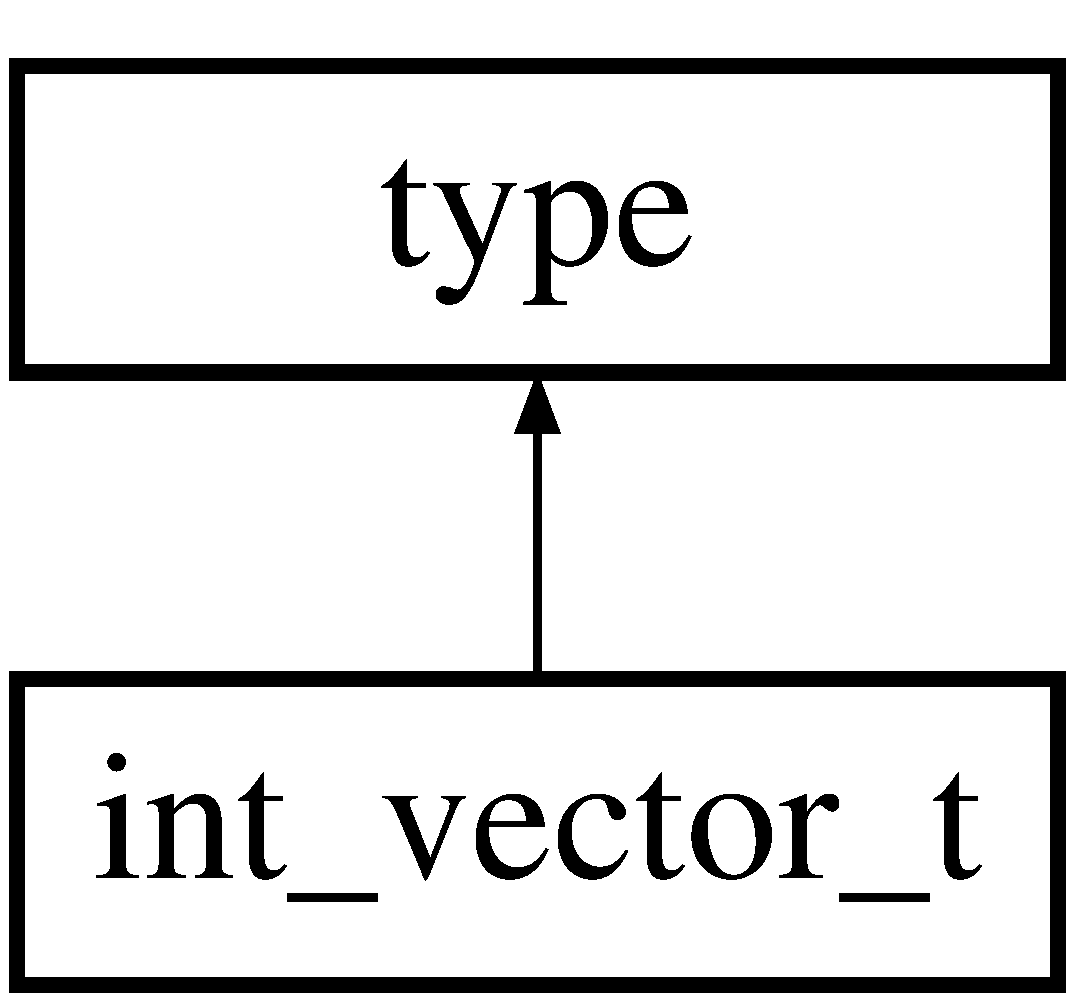
\includegraphics[height=2.000000cm]{classint__vector__t}
\end{center}
\end{figure}
\subsection*{Public Types}
\begin{DoxyCompactItemize}
\item 
typedef \+::\hyperlink{namespacexml__schema_acfa24ac68e1a188e7f44c36f7a158bf4}{xml\+\_\+schema\+::int\+\_\+} \hyperlink{classint__vector__t_a707ce51b5d31dcba928e26f41fa36cfa}{x\+\_\+type}
\item 
typedef \+::xsd\+::cxx\+::tree\+::traits$<$ \hyperlink{classint__vector__t_a707ce51b5d31dcba928e26f41fa36cfa}{x\+\_\+type}, char $>$ \hyperlink{classint__vector__t_a43010f516b3ee7806207d1234253c680}{x\+\_\+traits}
\item 
typedef \+::\hyperlink{namespacexml__schema_acfa24ac68e1a188e7f44c36f7a158bf4}{xml\+\_\+schema\+::int\+\_\+} \hyperlink{classint__vector__t_a7aa2a9276bdee3fad0e216343485a844}{y\+\_\+type}
\item 
typedef \+::xsd\+::cxx\+::tree\+::traits$<$ \hyperlink{classint__vector__t_a7aa2a9276bdee3fad0e216343485a844}{y\+\_\+type}, char $>$ \hyperlink{classint__vector__t_a2575b8ba0507d56caa435e393853e0ff}{y\+\_\+traits}
\item 
typedef \+::\hyperlink{namespacexml__schema_acfa24ac68e1a188e7f44c36f7a158bf4}{xml\+\_\+schema\+::int\+\_\+} \hyperlink{classint__vector__t_a20a60edf9f56f9455dc62b4e5f547bc3}{z\+\_\+type}
\item 
typedef \+::xsd\+::cxx\+::tree\+::traits$<$ \hyperlink{classint__vector__t_a20a60edf9f56f9455dc62b4e5f547bc3}{z\+\_\+type}, char $>$ \hyperlink{classint__vector__t_a867c91a38d505be5f9a8c1a72e4e48ba}{z\+\_\+traits}
\end{DoxyCompactItemize}
\subsection*{Public Member Functions}
\begin{DoxyCompactItemize}
\item 
const \hyperlink{classint__vector__t_a707ce51b5d31dcba928e26f41fa36cfa}{x\+\_\+type} \& \hyperlink{classint__vector__t_a594dd2055e5fe58eadb41177c23e406b}{x} () const 
\item 
\hyperlink{classint__vector__t_a707ce51b5d31dcba928e26f41fa36cfa}{x\+\_\+type} \& \hyperlink{classint__vector__t_ad5342135f1fddb1d291f2c8a60a1c891}{x} ()
\item 
void \hyperlink{classint__vector__t_af67370581e68faa8054d513e2616acca}{x} (const \hyperlink{classint__vector__t_a707ce51b5d31dcba928e26f41fa36cfa}{x\+\_\+type} \&x)
\item 
const \hyperlink{classint__vector__t_a7aa2a9276bdee3fad0e216343485a844}{y\+\_\+type} \& \hyperlink{classint__vector__t_a5b40d656ef8a62f880dc86098ae79649}{y} () const 
\item 
\hyperlink{classint__vector__t_a7aa2a9276bdee3fad0e216343485a844}{y\+\_\+type} \& \hyperlink{classint__vector__t_af2224a283e5b7d8e9b80e7f84290320a}{y} ()
\item 
void \hyperlink{classint__vector__t_ad01c94b1cafb22f5eeda8632113bea4a}{y} (const \hyperlink{classint__vector__t_a7aa2a9276bdee3fad0e216343485a844}{y\+\_\+type} \&\hyperlink{classint__vector__t_a594dd2055e5fe58eadb41177c23e406b}{x})
\item 
const \hyperlink{classint__vector__t_a20a60edf9f56f9455dc62b4e5f547bc3}{z\+\_\+type} \& \hyperlink{classint__vector__t_a636168acc3d1f5ded650d0f8f0a3b9e8}{z} () const 
\item 
\hyperlink{classint__vector__t_a20a60edf9f56f9455dc62b4e5f547bc3}{z\+\_\+type} \& \hyperlink{classint__vector__t_a917a6a9f765a4521ce9ce378b5fc4177}{z} ()
\item 
void \hyperlink{classint__vector__t_a43d15bdc3ac6f698ddb66ab586e1ecc1}{z} (const \hyperlink{classint__vector__t_a20a60edf9f56f9455dc62b4e5f547bc3}{z\+\_\+type} \&\hyperlink{classint__vector__t_a594dd2055e5fe58eadb41177c23e406b}{x})
\item 
\hyperlink{classint__vector__t_a7a5ff45f84e844e190bd6e41980bc365}{int\+\_\+vector\+\_\+t} (const \hyperlink{classint__vector__t_a707ce51b5d31dcba928e26f41fa36cfa}{x\+\_\+type} \&, const \hyperlink{classint__vector__t_a7aa2a9276bdee3fad0e216343485a844}{y\+\_\+type} \&, const \hyperlink{classint__vector__t_a20a60edf9f56f9455dc62b4e5f547bc3}{z\+\_\+type} \&)
\item 
\hyperlink{classint__vector__t_a4c3efd25f1ff338f305182b06ebceff2}{int\+\_\+vector\+\_\+t} (const \+::xercesc\+::\+D\+O\+M\+Element \&e,\+::\hyperlink{namespacexml__schema_a0612287d030cb2732d31a45b258fdc87}{xml\+\_\+schema\+::flags} f=0,\+::\hyperlink{namespacexml__schema_ada9aa30dc722e93ee2ed7243085402a5}{xml\+\_\+schema\+::container} $\ast$c=0)
\item 
\hyperlink{classint__vector__t_a6771bfa76a5b90f1909de20a08b06b9d}{int\+\_\+vector\+\_\+t} (const \hyperlink{classint__vector__t}{int\+\_\+vector\+\_\+t} \&\hyperlink{classint__vector__t_a594dd2055e5fe58eadb41177c23e406b}{x},\+::\hyperlink{namespacexml__schema_a0612287d030cb2732d31a45b258fdc87}{xml\+\_\+schema\+::flags} f=0,\+::\hyperlink{namespacexml__schema_ada9aa30dc722e93ee2ed7243085402a5}{xml\+\_\+schema\+::container} $\ast$c=0)
\item 
virtual \hyperlink{classint__vector__t}{int\+\_\+vector\+\_\+t} $\ast$ \hyperlink{classint__vector__t_a32c2f7c7b895ecd35059948b192538bf}{\+\_\+clone} (\+::\hyperlink{namespacexml__schema_a0612287d030cb2732d31a45b258fdc87}{xml\+\_\+schema\+::flags} f=0,\+::\hyperlink{namespacexml__schema_ada9aa30dc722e93ee2ed7243085402a5}{xml\+\_\+schema\+::container} $\ast$c=0) const 
\item 
\hyperlink{classint__vector__t}{int\+\_\+vector\+\_\+t} \& \hyperlink{classint__vector__t_a2d88328ab01a70176cea852e1c4bc877}{operator=} (const \hyperlink{classint__vector__t}{int\+\_\+vector\+\_\+t} \&\hyperlink{classint__vector__t_a594dd2055e5fe58eadb41177c23e406b}{x})
\item 
virtual \hyperlink{classint__vector__t_ab9f400a26a6d2e170f94972314a7f516}{$\sim$int\+\_\+vector\+\_\+t} ()
\end{DoxyCompactItemize}
\subsection*{Protected Member Functions}
\begin{DoxyCompactItemize}
\item 
void \hyperlink{classint__vector__t_ac351fecb08f5813010ac26d80be81d1b}{parse} (\+::xsd\+::cxx\+::xml\+::dom\+::parser$<$ char $>$ \&,\+::\hyperlink{namespacexml__schema_a0612287d030cb2732d31a45b258fdc87}{xml\+\_\+schema\+::flags})
\end{DoxyCompactItemize}
\subsection*{Protected Attributes}
\begin{DoxyCompactItemize}
\item 
\+::xsd\+::cxx\+::tree\+::one$<$ \hyperlink{classint__vector__t_a707ce51b5d31dcba928e26f41fa36cfa}{x\+\_\+type} $>$ \hyperlink{classint__vector__t_a2d1f7567a00dcd03634f576acf27ea93}{x\+\_\+}
\item 
\+::xsd\+::cxx\+::tree\+::one$<$ \hyperlink{classint__vector__t_a7aa2a9276bdee3fad0e216343485a844}{y\+\_\+type} $>$ \hyperlink{classint__vector__t_a2868a6aa13498be4826f4c76e37eeecc}{y\+\_\+}
\item 
\+::xsd\+::cxx\+::tree\+::one$<$ \hyperlink{classint__vector__t_a20a60edf9f56f9455dc62b4e5f547bc3}{z\+\_\+type} $>$ \hyperlink{classint__vector__t_ac10fc1d107a32a8515947d1aa4e29f3a}{z\+\_\+}
\end{DoxyCompactItemize}


\subsection{Member Typedef Documentation}
\index{int\+\_\+vector\+\_\+t@{int\+\_\+vector\+\_\+t}!x\+\_\+traits@{x\+\_\+traits}}
\index{x\+\_\+traits@{x\+\_\+traits}!int\+\_\+vector\+\_\+t@{int\+\_\+vector\+\_\+t}}
\subsubsection[{\texorpdfstring{x\+\_\+traits}{x_traits}}]{\setlength{\rightskip}{0pt plus 5cm}typedef \+::xsd\+::cxx\+::tree\+::traits$<$ {\bf x\+\_\+type}, char $>$ {\bf int\+\_\+vector\+\_\+t\+::x\+\_\+traits}}\hypertarget{classint__vector__t_a43010f516b3ee7806207d1234253c680}{}\label{classint__vector__t_a43010f516b3ee7806207d1234253c680}
\index{int\+\_\+vector\+\_\+t@{int\+\_\+vector\+\_\+t}!x\+\_\+type@{x\+\_\+type}}
\index{x\+\_\+type@{x\+\_\+type}!int\+\_\+vector\+\_\+t@{int\+\_\+vector\+\_\+t}}
\subsubsection[{\texorpdfstring{x\+\_\+type}{x_type}}]{\setlength{\rightskip}{0pt plus 5cm}typedef \+::{\bf xml\+\_\+schema\+::int\+\_\+} {\bf int\+\_\+vector\+\_\+t\+::x\+\_\+type}}\hypertarget{classint__vector__t_a707ce51b5d31dcba928e26f41fa36cfa}{}\label{classint__vector__t_a707ce51b5d31dcba928e26f41fa36cfa}
\index{int\+\_\+vector\+\_\+t@{int\+\_\+vector\+\_\+t}!y\+\_\+traits@{y\+\_\+traits}}
\index{y\+\_\+traits@{y\+\_\+traits}!int\+\_\+vector\+\_\+t@{int\+\_\+vector\+\_\+t}}
\subsubsection[{\texorpdfstring{y\+\_\+traits}{y_traits}}]{\setlength{\rightskip}{0pt plus 5cm}typedef \+::xsd\+::cxx\+::tree\+::traits$<$ {\bf y\+\_\+type}, char $>$ {\bf int\+\_\+vector\+\_\+t\+::y\+\_\+traits}}\hypertarget{classint__vector__t_a2575b8ba0507d56caa435e393853e0ff}{}\label{classint__vector__t_a2575b8ba0507d56caa435e393853e0ff}
\index{int\+\_\+vector\+\_\+t@{int\+\_\+vector\+\_\+t}!y\+\_\+type@{y\+\_\+type}}
\index{y\+\_\+type@{y\+\_\+type}!int\+\_\+vector\+\_\+t@{int\+\_\+vector\+\_\+t}}
\subsubsection[{\texorpdfstring{y\+\_\+type}{y_type}}]{\setlength{\rightskip}{0pt plus 5cm}typedef \+::{\bf xml\+\_\+schema\+::int\+\_\+} {\bf int\+\_\+vector\+\_\+t\+::y\+\_\+type}}\hypertarget{classint__vector__t_a7aa2a9276bdee3fad0e216343485a844}{}\label{classint__vector__t_a7aa2a9276bdee3fad0e216343485a844}
\index{int\+\_\+vector\+\_\+t@{int\+\_\+vector\+\_\+t}!z\+\_\+traits@{z\+\_\+traits}}
\index{z\+\_\+traits@{z\+\_\+traits}!int\+\_\+vector\+\_\+t@{int\+\_\+vector\+\_\+t}}
\subsubsection[{\texorpdfstring{z\+\_\+traits}{z_traits}}]{\setlength{\rightskip}{0pt plus 5cm}typedef \+::xsd\+::cxx\+::tree\+::traits$<$ {\bf z\+\_\+type}, char $>$ {\bf int\+\_\+vector\+\_\+t\+::z\+\_\+traits}}\hypertarget{classint__vector__t_a867c91a38d505be5f9a8c1a72e4e48ba}{}\label{classint__vector__t_a867c91a38d505be5f9a8c1a72e4e48ba}
\index{int\+\_\+vector\+\_\+t@{int\+\_\+vector\+\_\+t}!z\+\_\+type@{z\+\_\+type}}
\index{z\+\_\+type@{z\+\_\+type}!int\+\_\+vector\+\_\+t@{int\+\_\+vector\+\_\+t}}
\subsubsection[{\texorpdfstring{z\+\_\+type}{z_type}}]{\setlength{\rightskip}{0pt plus 5cm}typedef \+::{\bf xml\+\_\+schema\+::int\+\_\+} {\bf int\+\_\+vector\+\_\+t\+::z\+\_\+type}}\hypertarget{classint__vector__t_a20a60edf9f56f9455dc62b4e5f547bc3}{}\label{classint__vector__t_a20a60edf9f56f9455dc62b4e5f547bc3}


\subsection{Constructor \& Destructor Documentation}
\index{int\+\_\+vector\+\_\+t@{int\+\_\+vector\+\_\+t}!int\+\_\+vector\+\_\+t@{int\+\_\+vector\+\_\+t}}
\index{int\+\_\+vector\+\_\+t@{int\+\_\+vector\+\_\+t}!int\+\_\+vector\+\_\+t@{int\+\_\+vector\+\_\+t}}
\subsubsection[{\texorpdfstring{int\+\_\+vector\+\_\+t(const x\+\_\+type \&, const y\+\_\+type \&, const z\+\_\+type \&)}{int_vector_t(const x_type &, const y_type &, const z_type &)}}]{\setlength{\rightskip}{0pt plus 5cm}int\+\_\+vector\+\_\+t\+::int\+\_\+vector\+\_\+t (
\begin{DoxyParamCaption}
\item[{const {\bf x\+\_\+type} \&}]{x, }
\item[{const {\bf y\+\_\+type} \&}]{y, }
\item[{const {\bf z\+\_\+type} \&}]{z}
\end{DoxyParamCaption}
)}\hypertarget{classint__vector__t_a7a5ff45f84e844e190bd6e41980bc365}{}\label{classint__vector__t_a7a5ff45f84e844e190bd6e41980bc365}
\index{int\+\_\+vector\+\_\+t@{int\+\_\+vector\+\_\+t}!int\+\_\+vector\+\_\+t@{int\+\_\+vector\+\_\+t}}
\index{int\+\_\+vector\+\_\+t@{int\+\_\+vector\+\_\+t}!int\+\_\+vector\+\_\+t@{int\+\_\+vector\+\_\+t}}
\subsubsection[{\texorpdfstring{int\+\_\+vector\+\_\+t(const \+::xercesc\+::\+D\+O\+M\+Element \&e,\+::xml\+\_\+schema\+::flags f=0,\+::xml\+\_\+schema\+::container $\ast$c=0)}{int_vector_t(const ::xercesc::DOMElement &e,::xml_schema::flags f=0,::xml_schema::container *c=0)}}]{\setlength{\rightskip}{0pt plus 5cm}int\+\_\+vector\+\_\+t\+::int\+\_\+vector\+\_\+t (
\begin{DoxyParamCaption}
\item[{const \+::xercesc\+::\+D\+O\+M\+Element \&}]{e, }
\item[{\+::{\bf xml\+\_\+schema\+::flags}}]{f = {\ttfamily 0}, }
\item[{\+::{\bf xml\+\_\+schema\+::container} $\ast$}]{c = {\ttfamily 0}}
\end{DoxyParamCaption}
)}\hypertarget{classint__vector__t_a4c3efd25f1ff338f305182b06ebceff2}{}\label{classint__vector__t_a4c3efd25f1ff338f305182b06ebceff2}
\index{int\+\_\+vector\+\_\+t@{int\+\_\+vector\+\_\+t}!int\+\_\+vector\+\_\+t@{int\+\_\+vector\+\_\+t}}
\index{int\+\_\+vector\+\_\+t@{int\+\_\+vector\+\_\+t}!int\+\_\+vector\+\_\+t@{int\+\_\+vector\+\_\+t}}
\subsubsection[{\texorpdfstring{int\+\_\+vector\+\_\+t(const int\+\_\+vector\+\_\+t \&x,\+::xml\+\_\+schema\+::flags f=0,\+::xml\+\_\+schema\+::container $\ast$c=0)}{int_vector_t(const int_vector_t &x,::xml_schema::flags f=0,::xml_schema::container *c=0)}}]{\setlength{\rightskip}{0pt plus 5cm}int\+\_\+vector\+\_\+t\+::int\+\_\+vector\+\_\+t (
\begin{DoxyParamCaption}
\item[{const {\bf int\+\_\+vector\+\_\+t} \&}]{x, }
\item[{\+::{\bf xml\+\_\+schema\+::flags}}]{f = {\ttfamily 0}, }
\item[{\+::{\bf xml\+\_\+schema\+::container} $\ast$}]{c = {\ttfamily 0}}
\end{DoxyParamCaption}
)}\hypertarget{classint__vector__t_a6771bfa76a5b90f1909de20a08b06b9d}{}\label{classint__vector__t_a6771bfa76a5b90f1909de20a08b06b9d}
\index{int\+\_\+vector\+\_\+t@{int\+\_\+vector\+\_\+t}!````~int\+\_\+vector\+\_\+t@{$\sim$int\+\_\+vector\+\_\+t}}
\index{````~int\+\_\+vector\+\_\+t@{$\sim$int\+\_\+vector\+\_\+t}!int\+\_\+vector\+\_\+t@{int\+\_\+vector\+\_\+t}}
\subsubsection[{\texorpdfstring{$\sim$int\+\_\+vector\+\_\+t()}{~int_vector_t()}}]{\setlength{\rightskip}{0pt plus 5cm}int\+\_\+vector\+\_\+t\+::$\sim$int\+\_\+vector\+\_\+t (
\begin{DoxyParamCaption}
{}
\end{DoxyParamCaption}
)\hspace{0.3cm}{\ttfamily [virtual]}}\hypertarget{classint__vector__t_ab9f400a26a6d2e170f94972314a7f516}{}\label{classint__vector__t_ab9f400a26a6d2e170f94972314a7f516}


\subsection{Member Function Documentation}
\index{int\+\_\+vector\+\_\+t@{int\+\_\+vector\+\_\+t}!\+\_\+clone@{\+\_\+clone}}
\index{\+\_\+clone@{\+\_\+clone}!int\+\_\+vector\+\_\+t@{int\+\_\+vector\+\_\+t}}
\subsubsection[{\texorpdfstring{\+\_\+clone(\+::xml\+\_\+schema\+::flags f=0,\+::xml\+\_\+schema\+::container $\ast$c=0) const }{_clone(::xml_schema::flags f=0,::xml_schema::container *c=0) const }}]{\setlength{\rightskip}{0pt plus 5cm}{\bf int\+\_\+vector\+\_\+t} $\ast$ int\+\_\+vector\+\_\+t\+::\+\_\+clone (
\begin{DoxyParamCaption}
\item[{\+::{\bf xml\+\_\+schema\+::flags}}]{f = {\ttfamily 0}, }
\item[{\+::{\bf xml\+\_\+schema\+::container} $\ast$}]{c = {\ttfamily 0}}
\end{DoxyParamCaption}
) const\hspace{0.3cm}{\ttfamily [virtual]}}\hypertarget{classint__vector__t_a32c2f7c7b895ecd35059948b192538bf}{}\label{classint__vector__t_a32c2f7c7b895ecd35059948b192538bf}
\index{int\+\_\+vector\+\_\+t@{int\+\_\+vector\+\_\+t}!operator=@{operator=}}
\index{operator=@{operator=}!int\+\_\+vector\+\_\+t@{int\+\_\+vector\+\_\+t}}
\subsubsection[{\texorpdfstring{operator=(const int\+\_\+vector\+\_\+t \&x)}{operator=(const int_vector_t &x)}}]{\setlength{\rightskip}{0pt plus 5cm}{\bf int\+\_\+vector\+\_\+t} \& int\+\_\+vector\+\_\+t\+::operator= (
\begin{DoxyParamCaption}
\item[{const {\bf int\+\_\+vector\+\_\+t} \&}]{x}
\end{DoxyParamCaption}
)}\hypertarget{classint__vector__t_a2d88328ab01a70176cea852e1c4bc877}{}\label{classint__vector__t_a2d88328ab01a70176cea852e1c4bc877}
\index{int\+\_\+vector\+\_\+t@{int\+\_\+vector\+\_\+t}!parse@{parse}}
\index{parse@{parse}!int\+\_\+vector\+\_\+t@{int\+\_\+vector\+\_\+t}}
\subsubsection[{\texorpdfstring{parse(\+::xsd\+::cxx\+::xml\+::dom\+::parser$<$ char $>$ \&,\+::xml\+\_\+schema\+::flags)}{parse(::xsd::cxx::xml::dom::parser< char > &,::xml_schema::flags)}}]{\setlength{\rightskip}{0pt plus 5cm}void int\+\_\+vector\+\_\+t\+::parse (
\begin{DoxyParamCaption}
\item[{\+::xsd\+::cxx\+::xml\+::dom\+::parser$<$ char $>$ \&}]{p, }
\item[{\+::{\bf xml\+\_\+schema\+::flags}}]{f}
\end{DoxyParamCaption}
)\hspace{0.3cm}{\ttfamily [protected]}}\hypertarget{classint__vector__t_ac351fecb08f5813010ac26d80be81d1b}{}\label{classint__vector__t_ac351fecb08f5813010ac26d80be81d1b}
\index{int\+\_\+vector\+\_\+t@{int\+\_\+vector\+\_\+t}!x@{x}}
\index{x@{x}!int\+\_\+vector\+\_\+t@{int\+\_\+vector\+\_\+t}}
\subsubsection[{\texorpdfstring{x() const }{x() const }}]{\setlength{\rightskip}{0pt plus 5cm}const {\bf int\+\_\+vector\+\_\+t\+::x\+\_\+type} \& int\+\_\+vector\+\_\+t\+::x (
\begin{DoxyParamCaption}
{}
\end{DoxyParamCaption}
) const}\hypertarget{classint__vector__t_a594dd2055e5fe58eadb41177c23e406b}{}\label{classint__vector__t_a594dd2055e5fe58eadb41177c23e406b}
\index{int\+\_\+vector\+\_\+t@{int\+\_\+vector\+\_\+t}!x@{x}}
\index{x@{x}!int\+\_\+vector\+\_\+t@{int\+\_\+vector\+\_\+t}}
\subsubsection[{\texorpdfstring{x()}{x()}}]{\setlength{\rightskip}{0pt plus 5cm}{\bf int\+\_\+vector\+\_\+t\+::x\+\_\+type} \& int\+\_\+vector\+\_\+t\+::x (
\begin{DoxyParamCaption}
{}
\end{DoxyParamCaption}
)}\hypertarget{classint__vector__t_ad5342135f1fddb1d291f2c8a60a1c891}{}\label{classint__vector__t_ad5342135f1fddb1d291f2c8a60a1c891}
\index{int\+\_\+vector\+\_\+t@{int\+\_\+vector\+\_\+t}!x@{x}}
\index{x@{x}!int\+\_\+vector\+\_\+t@{int\+\_\+vector\+\_\+t}}
\subsubsection[{\texorpdfstring{x(const x\+\_\+type \&x)}{x(const x_type &x)}}]{\setlength{\rightskip}{0pt plus 5cm}void int\+\_\+vector\+\_\+t\+::x (
\begin{DoxyParamCaption}
\item[{const {\bf x\+\_\+type} \&}]{x}
\end{DoxyParamCaption}
)}\hypertarget{classint__vector__t_af67370581e68faa8054d513e2616acca}{}\label{classint__vector__t_af67370581e68faa8054d513e2616acca}
\index{int\+\_\+vector\+\_\+t@{int\+\_\+vector\+\_\+t}!y@{y}}
\index{y@{y}!int\+\_\+vector\+\_\+t@{int\+\_\+vector\+\_\+t}}
\subsubsection[{\texorpdfstring{y() const }{y() const }}]{\setlength{\rightskip}{0pt plus 5cm}const {\bf int\+\_\+vector\+\_\+t\+::y\+\_\+type} \& int\+\_\+vector\+\_\+t\+::y (
\begin{DoxyParamCaption}
{}
\end{DoxyParamCaption}
) const}\hypertarget{classint__vector__t_a5b40d656ef8a62f880dc86098ae79649}{}\label{classint__vector__t_a5b40d656ef8a62f880dc86098ae79649}
\index{int\+\_\+vector\+\_\+t@{int\+\_\+vector\+\_\+t}!y@{y}}
\index{y@{y}!int\+\_\+vector\+\_\+t@{int\+\_\+vector\+\_\+t}}
\subsubsection[{\texorpdfstring{y()}{y()}}]{\setlength{\rightskip}{0pt plus 5cm}{\bf int\+\_\+vector\+\_\+t\+::y\+\_\+type} \& int\+\_\+vector\+\_\+t\+::y (
\begin{DoxyParamCaption}
{}
\end{DoxyParamCaption}
)}\hypertarget{classint__vector__t_af2224a283e5b7d8e9b80e7f84290320a}{}\label{classint__vector__t_af2224a283e5b7d8e9b80e7f84290320a}
\index{int\+\_\+vector\+\_\+t@{int\+\_\+vector\+\_\+t}!y@{y}}
\index{y@{y}!int\+\_\+vector\+\_\+t@{int\+\_\+vector\+\_\+t}}
\subsubsection[{\texorpdfstring{y(const y\+\_\+type \&x)}{y(const y_type &x)}}]{\setlength{\rightskip}{0pt plus 5cm}void int\+\_\+vector\+\_\+t\+::y (
\begin{DoxyParamCaption}
\item[{const {\bf y\+\_\+type} \&}]{x}
\end{DoxyParamCaption}
)}\hypertarget{classint__vector__t_ad01c94b1cafb22f5eeda8632113bea4a}{}\label{classint__vector__t_ad01c94b1cafb22f5eeda8632113bea4a}
\index{int\+\_\+vector\+\_\+t@{int\+\_\+vector\+\_\+t}!z@{z}}
\index{z@{z}!int\+\_\+vector\+\_\+t@{int\+\_\+vector\+\_\+t}}
\subsubsection[{\texorpdfstring{z() const }{z() const }}]{\setlength{\rightskip}{0pt plus 5cm}const {\bf int\+\_\+vector\+\_\+t\+::z\+\_\+type} \& int\+\_\+vector\+\_\+t\+::z (
\begin{DoxyParamCaption}
{}
\end{DoxyParamCaption}
) const}\hypertarget{classint__vector__t_a636168acc3d1f5ded650d0f8f0a3b9e8}{}\label{classint__vector__t_a636168acc3d1f5ded650d0f8f0a3b9e8}
\index{int\+\_\+vector\+\_\+t@{int\+\_\+vector\+\_\+t}!z@{z}}
\index{z@{z}!int\+\_\+vector\+\_\+t@{int\+\_\+vector\+\_\+t}}
\subsubsection[{\texorpdfstring{z()}{z()}}]{\setlength{\rightskip}{0pt plus 5cm}{\bf int\+\_\+vector\+\_\+t\+::z\+\_\+type} \& int\+\_\+vector\+\_\+t\+::z (
\begin{DoxyParamCaption}
{}
\end{DoxyParamCaption}
)}\hypertarget{classint__vector__t_a917a6a9f765a4521ce9ce378b5fc4177}{}\label{classint__vector__t_a917a6a9f765a4521ce9ce378b5fc4177}
\index{int\+\_\+vector\+\_\+t@{int\+\_\+vector\+\_\+t}!z@{z}}
\index{z@{z}!int\+\_\+vector\+\_\+t@{int\+\_\+vector\+\_\+t}}
\subsubsection[{\texorpdfstring{z(const z\+\_\+type \&x)}{z(const z_type &x)}}]{\setlength{\rightskip}{0pt plus 5cm}void int\+\_\+vector\+\_\+t\+::z (
\begin{DoxyParamCaption}
\item[{const {\bf z\+\_\+type} \&}]{x}
\end{DoxyParamCaption}
)}\hypertarget{classint__vector__t_a43d15bdc3ac6f698ddb66ab586e1ecc1}{}\label{classint__vector__t_a43d15bdc3ac6f698ddb66ab586e1ecc1}


\subsection{Member Data Documentation}
\index{int\+\_\+vector\+\_\+t@{int\+\_\+vector\+\_\+t}!x\+\_\+@{x\+\_\+}}
\index{x\+\_\+@{x\+\_\+}!int\+\_\+vector\+\_\+t@{int\+\_\+vector\+\_\+t}}
\subsubsection[{\texorpdfstring{x\+\_\+}{x_}}]{\setlength{\rightskip}{0pt plus 5cm}\+::xsd\+::cxx\+::tree\+::one$<$ {\bf x\+\_\+type} $>$ int\+\_\+vector\+\_\+t\+::x\+\_\+\hspace{0.3cm}{\ttfamily [protected]}}\hypertarget{classint__vector__t_a2d1f7567a00dcd03634f576acf27ea93}{}\label{classint__vector__t_a2d1f7567a00dcd03634f576acf27ea93}
\index{int\+\_\+vector\+\_\+t@{int\+\_\+vector\+\_\+t}!y\+\_\+@{y\+\_\+}}
\index{y\+\_\+@{y\+\_\+}!int\+\_\+vector\+\_\+t@{int\+\_\+vector\+\_\+t}}
\subsubsection[{\texorpdfstring{y\+\_\+}{y_}}]{\setlength{\rightskip}{0pt plus 5cm}\+::xsd\+::cxx\+::tree\+::one$<$ {\bf y\+\_\+type} $>$ int\+\_\+vector\+\_\+t\+::y\+\_\+\hspace{0.3cm}{\ttfamily [protected]}}\hypertarget{classint__vector__t_a2868a6aa13498be4826f4c76e37eeecc}{}\label{classint__vector__t_a2868a6aa13498be4826f4c76e37eeecc}
\index{int\+\_\+vector\+\_\+t@{int\+\_\+vector\+\_\+t}!z\+\_\+@{z\+\_\+}}
\index{z\+\_\+@{z\+\_\+}!int\+\_\+vector\+\_\+t@{int\+\_\+vector\+\_\+t}}
\subsubsection[{\texorpdfstring{z\+\_\+}{z_}}]{\setlength{\rightskip}{0pt plus 5cm}\+::xsd\+::cxx\+::tree\+::one$<$ {\bf z\+\_\+type} $>$ int\+\_\+vector\+\_\+t\+::z\+\_\+\hspace{0.3cm}{\ttfamily [protected]}}\hypertarget{classint__vector__t_ac10fc1d107a32a8515947d1aa4e29f3a}{}\label{classint__vector__t_ac10fc1d107a32a8515947d1aa4e29f3a}


The documentation for this class was generated from the following files\+:\begin{DoxyCompactItemize}
\item 
src/input/\hyperlink{particle__input_8h}{particle\+\_\+input.\+h}\item 
src/input/\hyperlink{particle__input_8cpp}{particle\+\_\+input.\+cpp}\end{DoxyCompactItemize}

\hypertarget{classLinkedCellsContainer}{}\section{Linked\+Cells\+Container Class Reference}
\label{classLinkedCellsContainer}\index{Linked\+Cells\+Container@{Linked\+Cells\+Container}}


Class to hold cells containing a set of particles.  




{\ttfamily \#include $<$Linked\+Cells\+Container.\+h$>$}

Inheritance diagram for Linked\+Cells\+Container\+:\begin{figure}[H]
\begin{center}
\leavevmode
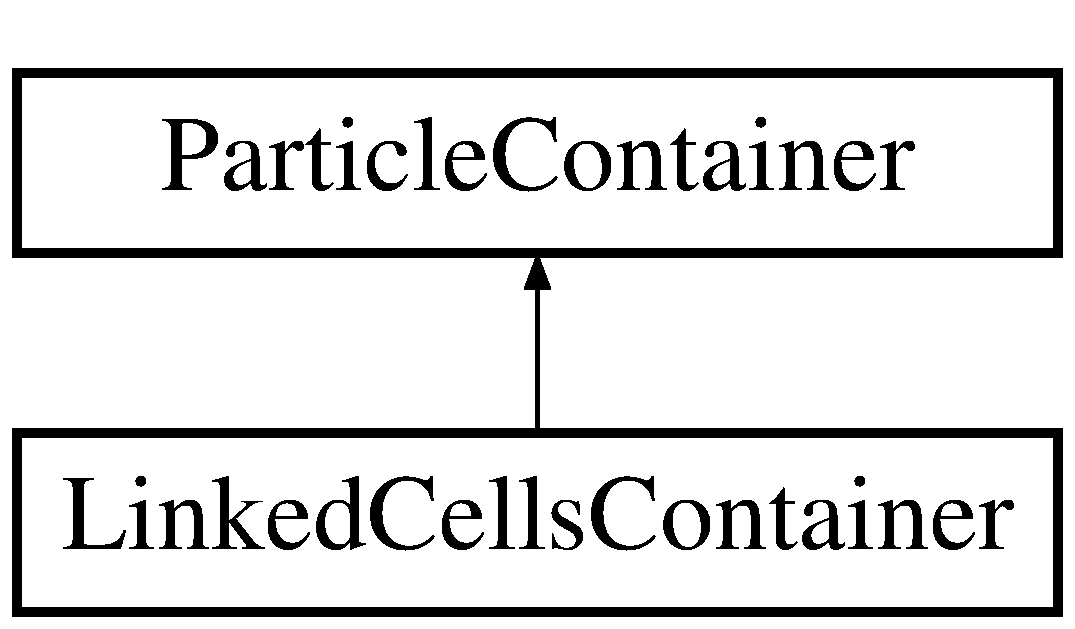
\includegraphics[height=2.000000cm]{classLinkedCellsContainer}
\end{center}
\end{figure}
\subsection*{Public Member Functions}
\begin{DoxyCompactItemize}
\item 
\hyperlink{classLinkedCellsContainer_ac2f170bf35d853298ca749527178de04}{Linked\+Cells\+Container} (\hyperlink{classParticleContainer_a2457078eafdf0fdd9eeb977e63aed6e8}{Force\+Method} \hyperlink{classParticleContainer_a839c3ff474bfece04fcbb0ca3fe9a0f8}{fm}, double timestep, double \hyperlink{classParticleContainer_a64e8a768554b5b6126755e8a8e85f2f5}{Brownian\+Factor}, double Rcutoff, double domainX, double domainY, double domainZ, \hyperlink{classutils_1_1Vector}{utils\+::\+Vector}$<$ int, 6 $>$ boundary, int threads=1)
\item 
virtual \hyperlink{classLinkedCellsContainer_aa59abdf61f50d80dc4b1a71fd727c3a9}{$\sim$\+Linked\+Cells\+Container} ()
\item 
void \hyperlink{classLinkedCellsContainer_a25d0ac927ce692ae3bf944a67f86682a}{set\+Gravity} (\hyperlink{classutils_1_1Vector}{utils\+::\+Vector}$<$ double, 3 $>$ g)
\item 
void \hyperlink{classLinkedCellsContainer_a968810914751bbc961b5c7ec33fab740}{set\+Domain} (double domainX, double domainY, double domainZ)
\item 
void \hyperlink{classLinkedCellsContainer_aad66003287011660d24817371eff4801}{set\+Mesh} (double Rcut, double domainX, double domainY, double domainZ)
\item 
void \hyperlink{classLinkedCellsContainer_a831a33f6b4f90f71396474a99f985575}{set\+Membrane} (double stiff, double r\+\_\+zero, bool status, double tend)
\item 
void \hyperlink{classLinkedCellsContainer_a0c54230125a031821a99fc39b15e6d60}{set\+List} (std\+::list$<$ \hyperlink{classParticle}{Particle} $>$ plist)
\item 
\hyperlink{classParticle}{Particle} $\ast$ \hyperlink{classLinkedCellsContainer_ac1987c930d49b2300a0f3509e282f2f1}{add\+Particle} (\hyperlink{classParticle}{Particle} \&p)
\item 
void \hyperlink{classLinkedCellsContainer_a6466835bf54973f4c7ec916c9b1f089b}{delete\+Particle} (\hyperlink{classParticle}{Particle} \&p)
\item 
std\+::list$<$ \hyperlink{classParticle}{Particle} $>$ \& \hyperlink{classLinkedCellsContainer_a33feabbd2ffc9f8cb34ec237e057b7bc}{get\+All} ()
\item 
virtual std\+::list$<$ \hyperlink{classParticle}{Particle} $\ast$ $>$ \hyperlink{classLinkedCellsContainer_a0b3b6c216a529189b58b05991079bb21}{get\+All\+Pointer} ()
\item 
std\+::list$<$ \hyperlink{classParticle}{Particle} $>$ \& \hyperlink{classLinkedCellsContainer_a89ebab6da4722ca5883899470183d7a3}{get\+Boundary} ()
\item 
std\+::list$<$ \hyperlink{classParticle}{Particle} $>$ \& \hyperlink{classLinkedCellsContainer_aaa470883e748eecb3f2409564402209d}{get\+Halo} ()
\item 
void \hyperlink{classLinkedCellsContainer_af8379a82b6aee0e2bc8b96db3a64f1fd}{clear\+Halo} ()
\item 
void \hyperlink{classLinkedCellsContainer_ae2ebc865c7e07122e2ab5985182d82bc}{f\+Reset} ()
\item 
void \hyperlink{classLinkedCellsContainer_a0dc45c921ad11aa2424b49ada44a0dfe}{test\+Force\+End} (double time)
\item 
void \hyperlink{classLinkedCellsContainer_a015b29c42c42a296b80775c225789f34}{Harmonic\+Potential} ()
\item 
void \hyperlink{classLinkedCellsContainer_a1975cb0083366555de77a734c0180125}{Reflecting\+Boundary} (\hyperlink{classParticle}{Particle} \&p, int i)
\item 
void \hyperlink{classLinkedCellsContainer_a0631cf4c5fbcf26b2f283634cbe0003b}{Periodic\+Boundary} ()
\item 
void \hyperlink{classLinkedCellsContainer_aaccb110aaed18cb2986a51e970e86fa4}{calculateF} ()
\item 
void \hyperlink{classLinkedCellsContainer_abacc626c54d71416ed4def4378fe74c4}{calculate\+Force\+For\+Cell} (int x, int y, int z)
\item 
void \hyperlink{classLinkedCellsContainer_ad2862569c3377347adfc06964ab7d966}{calculateX} ()
\item 
void \hyperlink{classLinkedCellsContainer_a5b9a6d9b726bda76160aaf7fbaffa821}{calculateV} ()
\end{DoxyCompactItemize}
\subsection*{Private Attributes}
\begin{DoxyCompactItemize}
\item 
int \hyperlink{classLinkedCellsContainer_a7e6ba97fe863d6dbcac93055f0945afc}{NcellsX}
\item 
int \hyperlink{classLinkedCellsContainer_a5d2caeb5e18c7691a7069d6d21ffb8f2}{NcellsY}
\item 
int \hyperlink{classLinkedCellsContainer_a422564396900533ee91d18fb9ead2c97}{NcellsZ}
\item 
int \hyperlink{classLinkedCellsContainer_a1e3adae4412e9e0e868dec802002d5ca}{Ncells\+XY}
\item 
int \hyperlink{classLinkedCellsContainer_a36307e254b1de62d27bbea099c244987}{Ncells\+Tot}
\item 
int \hyperlink{classLinkedCellsContainer_aa4b41b08627320b31ea4af06367901d1}{Max\+Dim}
\item 
int \hyperlink{classLinkedCellsContainer_ac8ae53015a3e5ed5bf413677dc3b506c}{Num\+Threads}
\item 
double \hyperlink{classLinkedCellsContainer_a6bf86e59ebe06054d1d118db261c2069}{HcellsX}
\item 
double \hyperlink{classLinkedCellsContainer_aa3c791c560dc1f5d3a5c8b48e0f93766}{HcellsY}
\item 
double \hyperlink{classLinkedCellsContainer_a5cd84e8209277710280e71becbaf7f65}{HcellsZ}
\item 
\hyperlink{classutils_1_1Vector}{utils\+::\+Vector}$<$ double, 3 $>$ \hyperlink{classLinkedCellsContainer_a9fed9ed73581f98ddc3cd3769b306937}{lowerleft}
\item 
\hyperlink{classutils_1_1Vector}{utils\+::\+Vector}$<$ double, 3 $>$ \hyperlink{classLinkedCellsContainer_a81d492dc2e1948839a6a45b0b1fe463f}{upperright}
\item 
std\+::vector$<$ \hyperlink{classParticleContainer}{Particle\+Container} $>$ \hyperlink{classLinkedCellsContainer_a71ab828ce5a0300256ce9d263dd03b71}{celllist}
\item 
\hyperlink{classutils_1_1Vector}{utils\+::\+Vector}$<$ int, 6 $>$ \hyperlink{classLinkedCellsContainer_a0f3e5cc44b3f152a4199c54e43b40d57}{Bound\+Cond}
\end{DoxyCompactItemize}
\subsection*{Additional Inherited Members}


\subsection{Detailed Description}
Class to hold cells containing a set of particles. 



\subsection{Constructor \& Destructor Documentation}
\index{Linked\+Cells\+Container@{Linked\+Cells\+Container}!Linked\+Cells\+Container@{Linked\+Cells\+Container}}
\index{Linked\+Cells\+Container@{Linked\+Cells\+Container}!Linked\+Cells\+Container@{Linked\+Cells\+Container}}
\subsubsection[{\texorpdfstring{Linked\+Cells\+Container(\+Force\+Method fm, double timestep, double Brownian\+Factor, double Rcutoff, double domain\+X, double domain\+Y, double domain\+Z, utils\+::\+Vector$<$ int, 6 $>$ boundary, int threads=1)}{LinkedCellsContainer(ForceMethod fm, double timestep, double BrownianFactor, double Rcutoff, double domainX, double domainY, double domainZ, utils::Vector< int, 6 > boundary, int threads=1)}}]{\setlength{\rightskip}{0pt plus 5cm}Linked\+Cells\+Container\+::\+Linked\+Cells\+Container (
\begin{DoxyParamCaption}
\item[{enum {\bf Particle\+Container\+::\+Force\+Method}}]{fm, }
\item[{double}]{timestep, }
\item[{double}]{Brownian\+Factor, }
\item[{double}]{Rcutoff, }
\item[{double}]{domainX, }
\item[{double}]{domainY, }
\item[{double}]{domainZ, }
\item[{{\bf utils\+::\+Vector}$<$ int, 6 $>$}]{boundary, }
\item[{int}]{threads = {\ttfamily 1}}
\end{DoxyParamCaption}
)}\hypertarget{classLinkedCellsContainer_ac2f170bf35d853298ca749527178de04}{}\label{classLinkedCellsContainer_ac2f170bf35d853298ca749527178de04}
Constructor 
\begin{DoxyParams}{Parameters}
{\em f} & Function function to calculate the force between two particles \\
\hline
{\em timestep} & time betweech each step \\
\hline
{\em Rcutoff} & only calculate forces between two particles if the distance is smaller than Rcutoff \\
\hline
{\em domainX} & x dimension of domain \\
\hline
{\em domainY} & y dimension of domain \\
\hline
{\em domainZ} & z dimension of domain \\
\hline
{\em boundary} & boundary conditions to be applied \\
\hline
{\em threads} & number of threads used for calculation \\
\hline
\end{DoxyParams}
\index{Linked\+Cells\+Container@{Linked\+Cells\+Container}!````~Linked\+Cells\+Container@{$\sim$\+Linked\+Cells\+Container}}
\index{````~Linked\+Cells\+Container@{$\sim$\+Linked\+Cells\+Container}!Linked\+Cells\+Container@{Linked\+Cells\+Container}}
\subsubsection[{\texorpdfstring{$\sim$\+Linked\+Cells\+Container()}{~LinkedCellsContainer()}}]{\setlength{\rightskip}{0pt plus 5cm}Linked\+Cells\+Container\+::$\sim$\+Linked\+Cells\+Container (
\begin{DoxyParamCaption}
{}
\end{DoxyParamCaption}
)\hspace{0.3cm}{\ttfamily [virtual]}}\hypertarget{classLinkedCellsContainer_aa59abdf61f50d80dc4b1a71fd727c3a9}{}\label{classLinkedCellsContainer_aa59abdf61f50d80dc4b1a71fd727c3a9}


\subsection{Member Function Documentation}
\index{Linked\+Cells\+Container@{Linked\+Cells\+Container}!add\+Particle@{add\+Particle}}
\index{add\+Particle@{add\+Particle}!Linked\+Cells\+Container@{Linked\+Cells\+Container}}
\subsubsection[{\texorpdfstring{add\+Particle(\+Particle \&p)}{addParticle(Particle &p)}}]{\setlength{\rightskip}{0pt plus 5cm}{\bf Particle} $\ast$ Linked\+Cells\+Container\+::add\+Particle (
\begin{DoxyParamCaption}
\item[{{\bf Particle} \&}]{p}
\end{DoxyParamCaption}
)\hspace{0.3cm}{\ttfamily [virtual]}}\hypertarget{classLinkedCellsContainer_ac1987c930d49b2300a0f3509e282f2f1}{}\label{classLinkedCellsContainer_ac1987c930d49b2300a0f3509e282f2f1}
add one particle to the container 
\begin{DoxyParams}{Parameters}
{\em p} & the particle to add \\
\hline
\end{DoxyParams}
\begin{DoxyReturn}{Returns}
a pointer to the particle 
\end{DoxyReturn}


Reimplemented from \hyperlink{classParticleContainer_a13b860c91defffff1404e8e3c12766a8}{Particle\+Container}.

\index{Linked\+Cells\+Container@{Linked\+Cells\+Container}!calculateF@{calculateF}}
\index{calculateF@{calculateF}!Linked\+Cells\+Container@{Linked\+Cells\+Container}}
\subsubsection[{\texorpdfstring{calculate\+F()}{calculateF()}}]{\setlength{\rightskip}{0pt plus 5cm}void Linked\+Cells\+Container\+::calculateF (
\begin{DoxyParamCaption}
{}
\end{DoxyParamCaption}
)\hspace{0.3cm}{\ttfamily [virtual]}}\hypertarget{classLinkedCellsContainer_aaccb110aaed18cb2986a51e970e86fa4}{}\label{classLinkedCellsContainer_aaccb110aaed18cb2986a51e970e86fa4}
calculate the force for all particles 

Reimplemented from \hyperlink{classParticleContainer_a329f1c21166cb9722553a1845f9be4d0}{Particle\+Container}.

\index{Linked\+Cells\+Container@{Linked\+Cells\+Container}!calculate\+Force\+For\+Cell@{calculate\+Force\+For\+Cell}}
\index{calculate\+Force\+For\+Cell@{calculate\+Force\+For\+Cell}!Linked\+Cells\+Container@{Linked\+Cells\+Container}}
\subsubsection[{\texorpdfstring{calculate\+Force\+For\+Cell(int x, int y, int z)}{calculateForceForCell(int x, int y, int z)}}]{\setlength{\rightskip}{0pt plus 5cm}void Linked\+Cells\+Container\+::calculate\+Force\+For\+Cell (
\begin{DoxyParamCaption}
\item[{int}]{x, }
\item[{int}]{y, }
\item[{int}]{z}
\end{DoxyParamCaption}
)}\hypertarget{classLinkedCellsContainer_abacc626c54d71416ed4def4378fe74c4}{}\label{classLinkedCellsContainer_abacc626c54d71416ed4def4378fe74c4}
calculate the force for given cell 
\begin{DoxyParams}{Parameters}
{\em x} & x-\/coord of cell \\
\hline
{\em y} & y-\/coord of cell \\
\hline
{\em z} & z-\/coord of cell \\
\hline
\end{DoxyParams}
\index{Linked\+Cells\+Container@{Linked\+Cells\+Container}!calculateV@{calculateV}}
\index{calculateV@{calculateV}!Linked\+Cells\+Container@{Linked\+Cells\+Container}}
\subsubsection[{\texorpdfstring{calculate\+V()}{calculateV()}}]{\setlength{\rightskip}{0pt plus 5cm}void Linked\+Cells\+Container\+::calculateV (
\begin{DoxyParamCaption}
{}
\end{DoxyParamCaption}
)\hspace{0.3cm}{\ttfamily [virtual]}}\hypertarget{classLinkedCellsContainer_a5b9a6d9b726bda76160aaf7fbaffa821}{}\label{classLinkedCellsContainer_a5b9a6d9b726bda76160aaf7fbaffa821}
calculate the position for all particles using the Velocity-\/\+Stoermer-\/\+Verlet-\/\+Algorithm 

Reimplemented from \hyperlink{classParticleContainer_a7b436c3226f9eb05e86d895a7eab8b41}{Particle\+Container}.

\index{Linked\+Cells\+Container@{Linked\+Cells\+Container}!calculateX@{calculateX}}
\index{calculateX@{calculateX}!Linked\+Cells\+Container@{Linked\+Cells\+Container}}
\subsubsection[{\texorpdfstring{calculate\+X()}{calculateX()}}]{\setlength{\rightskip}{0pt plus 5cm}void Linked\+Cells\+Container\+::calculateX (
\begin{DoxyParamCaption}
{}
\end{DoxyParamCaption}
)\hspace{0.3cm}{\ttfamily [virtual]}}\hypertarget{classLinkedCellsContainer_ad2862569c3377347adfc06964ab7d966}{}\label{classLinkedCellsContainer_ad2862569c3377347adfc06964ab7d966}
calculate the position for all particles using the Velocity-\/\+Stoermer-\/\+Verlet-\/\+Algorithm 

Reimplemented from \hyperlink{classParticleContainer_abfe567934c1e3319a03377ebf7da2369}{Particle\+Container}.

\index{Linked\+Cells\+Container@{Linked\+Cells\+Container}!clear\+Halo@{clear\+Halo}}
\index{clear\+Halo@{clear\+Halo}!Linked\+Cells\+Container@{Linked\+Cells\+Container}}
\subsubsection[{\texorpdfstring{clear\+Halo()}{clearHalo()}}]{\setlength{\rightskip}{0pt plus 5cm}void Linked\+Cells\+Container\+::clear\+Halo (
\begin{DoxyParamCaption}
{}
\end{DoxyParamCaption}
)}\hypertarget{classLinkedCellsContainer_af8379a82b6aee0e2bc8b96db3a64f1fd}{}\label{classLinkedCellsContainer_af8379a82b6aee0e2bc8b96db3a64f1fd}
delete all particles in halo \index{Linked\+Cells\+Container@{Linked\+Cells\+Container}!delete\+Particle@{delete\+Particle}}
\index{delete\+Particle@{delete\+Particle}!Linked\+Cells\+Container@{Linked\+Cells\+Container}}
\subsubsection[{\texorpdfstring{delete\+Particle(\+Particle \&p)}{deleteParticle(Particle &p)}}]{\setlength{\rightskip}{0pt plus 5cm}void Linked\+Cells\+Container\+::delete\+Particle (
\begin{DoxyParamCaption}
\item[{{\bf Particle} \&}]{p}
\end{DoxyParamCaption}
)\hspace{0.3cm}{\ttfamily [virtual]}}\hypertarget{classLinkedCellsContainer_a6466835bf54973f4c7ec916c9b1f089b}{}\label{classLinkedCellsContainer_a6466835bf54973f4c7ec916c9b1f089b}
remove a particle from the container 
\begin{DoxyParams}{Parameters}
{\em p} & the particle to remove \\
\hline
\end{DoxyParams}


Reimplemented from \hyperlink{classParticleContainer_a27c73f4106a4e38382dbf461e03bb5f1}{Particle\+Container}.

\index{Linked\+Cells\+Container@{Linked\+Cells\+Container}!f\+Reset@{f\+Reset}}
\index{f\+Reset@{f\+Reset}!Linked\+Cells\+Container@{Linked\+Cells\+Container}}
\subsubsection[{\texorpdfstring{f\+Reset()}{fReset()}}]{\setlength{\rightskip}{0pt plus 5cm}void Linked\+Cells\+Container\+::f\+Reset (
\begin{DoxyParamCaption}
{}
\end{DoxyParamCaption}
)\hspace{0.3cm}{\ttfamily [virtual]}}\hypertarget{classLinkedCellsContainer_ae2ebc865c7e07122e2ab5985182d82bc}{}\label{classLinkedCellsContainer_ae2ebc865c7e07122e2ab5985182d82bc}
set the force to all particles according to gravity force 

Reimplemented from \hyperlink{classParticleContainer_af5626526d41510605c20161df34de71b}{Particle\+Container}.

\index{Linked\+Cells\+Container@{Linked\+Cells\+Container}!get\+All@{get\+All}}
\index{get\+All@{get\+All}!Linked\+Cells\+Container@{Linked\+Cells\+Container}}
\subsubsection[{\texorpdfstring{get\+All()}{getAll()}}]{\setlength{\rightskip}{0pt plus 5cm}std\+::list$<$ {\bf Particle} $>$ \& Linked\+Cells\+Container\+::get\+All (
\begin{DoxyParamCaption}
{}
\end{DoxyParamCaption}
)\hspace{0.3cm}{\ttfamily [virtual]}}\hypertarget{classLinkedCellsContainer_a33feabbd2ffc9f8cb34ec237e057b7bc}{}\label{classLinkedCellsContainer_a33feabbd2ffc9f8cb34ec237e057b7bc}
get a list of all particle in the container \begin{DoxyReturn}{Returns}
list of all particles 
\end{DoxyReturn}


Reimplemented from \hyperlink{classParticleContainer_a5b96e023a5b3c2507766cefa8f006c65}{Particle\+Container}.

\index{Linked\+Cells\+Container@{Linked\+Cells\+Container}!get\+All\+Pointer@{get\+All\+Pointer}}
\index{get\+All\+Pointer@{get\+All\+Pointer}!Linked\+Cells\+Container@{Linked\+Cells\+Container}}
\subsubsection[{\texorpdfstring{get\+All\+Pointer()}{getAllPointer()}}]{\setlength{\rightskip}{0pt plus 5cm}std\+::list$<$ {\bf Particle} $\ast$ $>$ Linked\+Cells\+Container\+::get\+All\+Pointer (
\begin{DoxyParamCaption}
{}
\end{DoxyParamCaption}
)\hspace{0.3cm}{\ttfamily [virtual]}}\hypertarget{classLinkedCellsContainer_a0b3b6c216a529189b58b05991079bb21}{}\label{classLinkedCellsContainer_a0b3b6c216a529189b58b05991079bb21}
get a list of pointer to all particle in the container \begin{DoxyReturn}{Returns}
list of all particles 
\end{DoxyReturn}


Reimplemented from \hyperlink{classParticleContainer_a52ebfc06d0daa96fbeef945b43e4fe00}{Particle\+Container}.

\index{Linked\+Cells\+Container@{Linked\+Cells\+Container}!get\+Boundary@{get\+Boundary}}
\index{get\+Boundary@{get\+Boundary}!Linked\+Cells\+Container@{Linked\+Cells\+Container}}
\subsubsection[{\texorpdfstring{get\+Boundary()}{getBoundary()}}]{\setlength{\rightskip}{0pt plus 5cm}std\+::list$<$ {\bf Particle} $>$ \& Linked\+Cells\+Container\+::get\+Boundary (
\begin{DoxyParamCaption}
{}
\end{DoxyParamCaption}
)}\hypertarget{classLinkedCellsContainer_a89ebab6da4722ca5883899470183d7a3}{}\label{classLinkedCellsContainer_a89ebab6da4722ca5883899470183d7a3}
get a list of all particle in the boundary \begin{DoxyReturn}{Returns}
list of all particles 
\end{DoxyReturn}
\index{Linked\+Cells\+Container@{Linked\+Cells\+Container}!get\+Halo@{get\+Halo}}
\index{get\+Halo@{get\+Halo}!Linked\+Cells\+Container@{Linked\+Cells\+Container}}
\subsubsection[{\texorpdfstring{get\+Halo()}{getHalo()}}]{\setlength{\rightskip}{0pt plus 5cm}std\+::list$<$ {\bf Particle} $>$ \& Linked\+Cells\+Container\+::get\+Halo (
\begin{DoxyParamCaption}
{}
\end{DoxyParamCaption}
)}\hypertarget{classLinkedCellsContainer_aaa470883e748eecb3f2409564402209d}{}\label{classLinkedCellsContainer_aaa470883e748eecb3f2409564402209d}
get a list of all particle in the halo \begin{DoxyReturn}{Returns}
list of all particles 
\end{DoxyReturn}
\index{Linked\+Cells\+Container@{Linked\+Cells\+Container}!Harmonic\+Potential@{Harmonic\+Potential}}
\index{Harmonic\+Potential@{Harmonic\+Potential}!Linked\+Cells\+Container@{Linked\+Cells\+Container}}
\subsubsection[{\texorpdfstring{Harmonic\+Potential()}{HarmonicPotential()}}]{\setlength{\rightskip}{0pt plus 5cm}void Linked\+Cells\+Container\+::\+Harmonic\+Potential (
\begin{DoxyParamCaption}
{}
\end{DoxyParamCaption}
)}\hypertarget{classLinkedCellsContainer_a015b29c42c42a296b80775c225789f34}{}\label{classLinkedCellsContainer_a015b29c42c42a296b80775c225789f34}
computes the forces in a membrane \index{Linked\+Cells\+Container@{Linked\+Cells\+Container}!Periodic\+Boundary@{Periodic\+Boundary}}
\index{Periodic\+Boundary@{Periodic\+Boundary}!Linked\+Cells\+Container@{Linked\+Cells\+Container}}
\subsubsection[{\texorpdfstring{Periodic\+Boundary()}{PeriodicBoundary()}}]{\setlength{\rightskip}{0pt plus 5cm}void Linked\+Cells\+Container\+::\+Periodic\+Boundary (
\begin{DoxyParamCaption}
{}
\end{DoxyParamCaption}
)}\hypertarget{classLinkedCellsContainer_a0631cf4c5fbcf26b2f283634cbe0003b}{}\label{classLinkedCellsContainer_a0631cf4c5fbcf26b2f283634cbe0003b}
creates halo particle for particles on the boundary \index{Linked\+Cells\+Container@{Linked\+Cells\+Container}!Reflecting\+Boundary@{Reflecting\+Boundary}}
\index{Reflecting\+Boundary@{Reflecting\+Boundary}!Linked\+Cells\+Container@{Linked\+Cells\+Container}}
\subsubsection[{\texorpdfstring{Reflecting\+Boundary(\+Particle \&p, int i)}{ReflectingBoundary(Particle &p, int i)}}]{\setlength{\rightskip}{0pt plus 5cm}void Linked\+Cells\+Container\+::\+Reflecting\+Boundary (
\begin{DoxyParamCaption}
\item[{{\bf Particle} \&}]{p, }
\item[{int}]{i}
\end{DoxyParamCaption}
)}\hypertarget{classLinkedCellsContainer_a1975cb0083366555de77a734c0180125}{}\label{classLinkedCellsContainer_a1975cb0083366555de77a734c0180125}
applies the reflecting boundary condition 
\begin{DoxyParams}{Parameters}
{\em p} & the particle near the border \\
\hline
{\em i} & the cell index of the current cell \\
\hline
\end{DoxyParams}
\index{Linked\+Cells\+Container@{Linked\+Cells\+Container}!set\+Domain@{set\+Domain}}
\index{set\+Domain@{set\+Domain}!Linked\+Cells\+Container@{Linked\+Cells\+Container}}
\subsubsection[{\texorpdfstring{set\+Domain(double domain\+X, double domain\+Y, double domain\+Z)}{setDomain(double domainX, double domainY, double domainZ)}}]{\setlength{\rightskip}{0pt plus 5cm}void Linked\+Cells\+Container\+::set\+Domain (
\begin{DoxyParamCaption}
\item[{double}]{domainX, }
\item[{double}]{domainY, }
\item[{double}]{domainZ}
\end{DoxyParamCaption}
)}\hypertarget{classLinkedCellsContainer_a968810914751bbc961b5c7ec33fab740}{}\label{classLinkedCellsContainer_a968810914751bbc961b5c7ec33fab740}
set domain 
\begin{DoxyParams}{Parameters}
{\em x} & position vector of the lower left front-\/side corner \\
\hline
{\em domainX} & X-\/size of the domain \\
\hline
{\em domainY} & Y-\/size of the domain \\
\hline
\end{DoxyParams}
\index{Linked\+Cells\+Container@{Linked\+Cells\+Container}!set\+Gravity@{set\+Gravity}}
\index{set\+Gravity@{set\+Gravity}!Linked\+Cells\+Container@{Linked\+Cells\+Container}}
\subsubsection[{\texorpdfstring{set\+Gravity(utils\+::\+Vector$<$ double, 3 $>$ g)}{setGravity(utils::Vector< double, 3 > g)}}]{\setlength{\rightskip}{0pt plus 5cm}void Linked\+Cells\+Container\+::set\+Gravity (
\begin{DoxyParamCaption}
\item[{{\bf utils\+::\+Vector}$<$ double, 3 $>$}]{g}
\end{DoxyParamCaption}
)\hspace{0.3cm}{\ttfamily [virtual]}}\hypertarget{classLinkedCellsContainer_a25d0ac927ce692ae3bf944a67f86682a}{}\label{classLinkedCellsContainer_a25d0ac927ce692ae3bf944a67f86682a}
set the gravitational force along the z-\/axis 
\begin{DoxyParams}{Parameters}
{\em g} & the gravitational acceleration \\
\hline
\end{DoxyParams}


Reimplemented from \hyperlink{classParticleContainer_af7fe938fddd10136945f99625e141149}{Particle\+Container}.

\index{Linked\+Cells\+Container@{Linked\+Cells\+Container}!set\+List@{set\+List}}
\index{set\+List@{set\+List}!Linked\+Cells\+Container@{Linked\+Cells\+Container}}
\subsubsection[{\texorpdfstring{set\+List(std\+::list$<$ Particle $>$ plist)}{setList(std::list< Particle > plist)}}]{\setlength{\rightskip}{0pt plus 5cm}void Linked\+Cells\+Container\+::set\+List (
\begin{DoxyParamCaption}
\item[{std\+::list$<$ {\bf Particle} $>$}]{plist}
\end{DoxyParamCaption}
)\hspace{0.3cm}{\ttfamily [virtual]}}\hypertarget{classLinkedCellsContainer_a0c54230125a031821a99fc39b15e6d60}{}\label{classLinkedCellsContainer_a0c54230125a031821a99fc39b15e6d60}
define all particles in the container 
\begin{DoxyParams}{Parameters}
{\em plist} & the list to fill container \\
\hline
\end{DoxyParams}


Reimplemented from \hyperlink{classParticleContainer_ae3f61f4d99b06782cfd978779ccc13bf}{Particle\+Container}.

\index{Linked\+Cells\+Container@{Linked\+Cells\+Container}!set\+Membrane@{set\+Membrane}}
\index{set\+Membrane@{set\+Membrane}!Linked\+Cells\+Container@{Linked\+Cells\+Container}}
\subsubsection[{\texorpdfstring{set\+Membrane(double stiff, double r\+\_\+zero, bool status, double tend)}{setMembrane(double stiff, double r_zero, bool status, double tend)}}]{\setlength{\rightskip}{0pt plus 5cm}void Linked\+Cells\+Container\+::set\+Membrane (
\begin{DoxyParamCaption}
\item[{double}]{stiff, }
\item[{double}]{r\+\_\+zero, }
\item[{bool}]{status, }
\item[{double}]{tend}
\end{DoxyParamCaption}
)\hspace{0.3cm}{\ttfamily [virtual]}}\hypertarget{classLinkedCellsContainer_a831a33f6b4f90f71396474a99f985575}{}\label{classLinkedCellsContainer_a831a33f6b4f90f71396474a99f985575}
sets he membrane parameters to all cells 
\begin{DoxyParams}{Parameters}
{\em stiff} & membrane stiffness \\
\hline
{\em r\+\_\+ero} & average bond lenght \\
\hline
{\em status} & whether the membrane is active or not \\
\hline
{\em tend} & membrane t\+\_\+end \\
\hline
\end{DoxyParams}


Reimplemented from \hyperlink{classParticleContainer_abdd289393fe11f1192a9eb79b01b2680}{Particle\+Container}.

\index{Linked\+Cells\+Container@{Linked\+Cells\+Container}!set\+Mesh@{set\+Mesh}}
\index{set\+Mesh@{set\+Mesh}!Linked\+Cells\+Container@{Linked\+Cells\+Container}}
\subsubsection[{\texorpdfstring{set\+Mesh(double Rcut, double domain\+X, double domain\+Y, double domain\+Z)}{setMesh(double Rcut, double domainX, double domainY, double domainZ)}}]{\setlength{\rightskip}{0pt plus 5cm}void Linked\+Cells\+Container\+::set\+Mesh (
\begin{DoxyParamCaption}
\item[{double}]{Rcut, }
\item[{double}]{domainX, }
\item[{double}]{domainY, }
\item[{double}]{domainZ}
\end{DoxyParamCaption}
)}\hypertarget{classLinkedCellsContainer_aad66003287011660d24817371eff4801}{}\label{classLinkedCellsContainer_aad66003287011660d24817371eff4801}
set the cell mesh 
\begin{DoxyParams}{Parameters}
{\em Rcutoff} & the cut-\/off radius in the simulation \\
\hline
{\em Domain} & the domain for our simulation \\
\hline
\end{DoxyParams}
\index{Linked\+Cells\+Container@{Linked\+Cells\+Container}!test\+Force\+End@{test\+Force\+End}}
\index{test\+Force\+End@{test\+Force\+End}!Linked\+Cells\+Container@{Linked\+Cells\+Container}}
\subsubsection[{\texorpdfstring{test\+Force\+End(double time)}{testForceEnd(double time)}}]{\setlength{\rightskip}{0pt plus 5cm}void Linked\+Cells\+Container\+::test\+Force\+End (
\begin{DoxyParamCaption}
\item[{double}]{time}
\end{DoxyParamCaption}
)\hspace{0.3cm}{\ttfamily [virtual]}}\hypertarget{classLinkedCellsContainer_a0dc45c921ad11aa2424b49ada44a0dfe}{}\label{classLinkedCellsContainer_a0dc45c921ad11aa2424b49ada44a0dfe}
tests if the force up should be switched of 
\begin{DoxyParams}{Parameters}
{\em time} & current simulation time \\
\hline
\end{DoxyParams}


Reimplemented from \hyperlink{classParticleContainer_ae132e846bb2763712d4acca3095bcbfc}{Particle\+Container}.



\subsection{Member Data Documentation}
\index{Linked\+Cells\+Container@{Linked\+Cells\+Container}!Bound\+Cond@{Bound\+Cond}}
\index{Bound\+Cond@{Bound\+Cond}!Linked\+Cells\+Container@{Linked\+Cells\+Container}}
\subsubsection[{\texorpdfstring{Bound\+Cond}{BoundCond}}]{\setlength{\rightskip}{0pt plus 5cm}{\bf utils\+::\+Vector}$<$int,6$>$ Linked\+Cells\+Container\+::\+Bound\+Cond\hspace{0.3cm}{\ttfamily [private]}}\hypertarget{classLinkedCellsContainer_a0f3e5cc44b3f152a4199c54e43b40d57}{}\label{classLinkedCellsContainer_a0f3e5cc44b3f152a4199c54e43b40d57}
\index{Linked\+Cells\+Container@{Linked\+Cells\+Container}!celllist@{celllist}}
\index{celllist@{celllist}!Linked\+Cells\+Container@{Linked\+Cells\+Container}}
\subsubsection[{\texorpdfstring{celllist}{celllist}}]{\setlength{\rightskip}{0pt plus 5cm}std\+::vector$<${\bf Particle\+Container}$>$ Linked\+Cells\+Container\+::celllist\hspace{0.3cm}{\ttfamily [private]}}\hypertarget{classLinkedCellsContainer_a71ab828ce5a0300256ce9d263dd03b71}{}\label{classLinkedCellsContainer_a71ab828ce5a0300256ce9d263dd03b71}
\index{Linked\+Cells\+Container@{Linked\+Cells\+Container}!HcellsX@{HcellsX}}
\index{HcellsX@{HcellsX}!Linked\+Cells\+Container@{Linked\+Cells\+Container}}
\subsubsection[{\texorpdfstring{HcellsX}{HcellsX}}]{\setlength{\rightskip}{0pt plus 5cm}double Linked\+Cells\+Container\+::\+HcellsX\hspace{0.3cm}{\ttfamily [private]}}\hypertarget{classLinkedCellsContainer_a6bf86e59ebe06054d1d118db261c2069}{}\label{classLinkedCellsContainer_a6bf86e59ebe06054d1d118db261c2069}
\index{Linked\+Cells\+Container@{Linked\+Cells\+Container}!HcellsY@{HcellsY}}
\index{HcellsY@{HcellsY}!Linked\+Cells\+Container@{Linked\+Cells\+Container}}
\subsubsection[{\texorpdfstring{HcellsY}{HcellsY}}]{\setlength{\rightskip}{0pt plus 5cm}double Linked\+Cells\+Container\+::\+HcellsY\hspace{0.3cm}{\ttfamily [private]}}\hypertarget{classLinkedCellsContainer_aa3c791c560dc1f5d3a5c8b48e0f93766}{}\label{classLinkedCellsContainer_aa3c791c560dc1f5d3a5c8b48e0f93766}
\index{Linked\+Cells\+Container@{Linked\+Cells\+Container}!HcellsZ@{HcellsZ}}
\index{HcellsZ@{HcellsZ}!Linked\+Cells\+Container@{Linked\+Cells\+Container}}
\subsubsection[{\texorpdfstring{HcellsZ}{HcellsZ}}]{\setlength{\rightskip}{0pt plus 5cm}double Linked\+Cells\+Container\+::\+HcellsZ\hspace{0.3cm}{\ttfamily [private]}}\hypertarget{classLinkedCellsContainer_a5cd84e8209277710280e71becbaf7f65}{}\label{classLinkedCellsContainer_a5cd84e8209277710280e71becbaf7f65}
\index{Linked\+Cells\+Container@{Linked\+Cells\+Container}!lowerleft@{lowerleft}}
\index{lowerleft@{lowerleft}!Linked\+Cells\+Container@{Linked\+Cells\+Container}}
\subsubsection[{\texorpdfstring{lowerleft}{lowerleft}}]{\setlength{\rightskip}{0pt plus 5cm}{\bf utils\+::\+Vector}$<$double,3$>$ Linked\+Cells\+Container\+::lowerleft\hspace{0.3cm}{\ttfamily [private]}}\hypertarget{classLinkedCellsContainer_a9fed9ed73581f98ddc3cd3769b306937}{}\label{classLinkedCellsContainer_a9fed9ed73581f98ddc3cd3769b306937}
\index{Linked\+Cells\+Container@{Linked\+Cells\+Container}!Max\+Dim@{Max\+Dim}}
\index{Max\+Dim@{Max\+Dim}!Linked\+Cells\+Container@{Linked\+Cells\+Container}}
\subsubsection[{\texorpdfstring{Max\+Dim}{MaxDim}}]{\setlength{\rightskip}{0pt plus 5cm}int Linked\+Cells\+Container\+::\+Max\+Dim\hspace{0.3cm}{\ttfamily [private]}}\hypertarget{classLinkedCellsContainer_aa4b41b08627320b31ea4af06367901d1}{}\label{classLinkedCellsContainer_aa4b41b08627320b31ea4af06367901d1}
\index{Linked\+Cells\+Container@{Linked\+Cells\+Container}!Ncells\+Tot@{Ncells\+Tot}}
\index{Ncells\+Tot@{Ncells\+Tot}!Linked\+Cells\+Container@{Linked\+Cells\+Container}}
\subsubsection[{\texorpdfstring{Ncells\+Tot}{NcellsTot}}]{\setlength{\rightskip}{0pt plus 5cm}int Linked\+Cells\+Container\+::\+Ncells\+Tot\hspace{0.3cm}{\ttfamily [private]}}\hypertarget{classLinkedCellsContainer_a36307e254b1de62d27bbea099c244987}{}\label{classLinkedCellsContainer_a36307e254b1de62d27bbea099c244987}
\index{Linked\+Cells\+Container@{Linked\+Cells\+Container}!NcellsX@{NcellsX}}
\index{NcellsX@{NcellsX}!Linked\+Cells\+Container@{Linked\+Cells\+Container}}
\subsubsection[{\texorpdfstring{NcellsX}{NcellsX}}]{\setlength{\rightskip}{0pt plus 5cm}int Linked\+Cells\+Container\+::\+NcellsX\hspace{0.3cm}{\ttfamily [private]}}\hypertarget{classLinkedCellsContainer_a7e6ba97fe863d6dbcac93055f0945afc}{}\label{classLinkedCellsContainer_a7e6ba97fe863d6dbcac93055f0945afc}
\index{Linked\+Cells\+Container@{Linked\+Cells\+Container}!Ncells\+XY@{Ncells\+XY}}
\index{Ncells\+XY@{Ncells\+XY}!Linked\+Cells\+Container@{Linked\+Cells\+Container}}
\subsubsection[{\texorpdfstring{Ncells\+XY}{NcellsXY}}]{\setlength{\rightskip}{0pt plus 5cm}int Linked\+Cells\+Container\+::\+Ncells\+XY\hspace{0.3cm}{\ttfamily [private]}}\hypertarget{classLinkedCellsContainer_a1e3adae4412e9e0e868dec802002d5ca}{}\label{classLinkedCellsContainer_a1e3adae4412e9e0e868dec802002d5ca}
\index{Linked\+Cells\+Container@{Linked\+Cells\+Container}!NcellsY@{NcellsY}}
\index{NcellsY@{NcellsY}!Linked\+Cells\+Container@{Linked\+Cells\+Container}}
\subsubsection[{\texorpdfstring{NcellsY}{NcellsY}}]{\setlength{\rightskip}{0pt plus 5cm}int Linked\+Cells\+Container\+::\+NcellsY\hspace{0.3cm}{\ttfamily [private]}}\hypertarget{classLinkedCellsContainer_a5d2caeb5e18c7691a7069d6d21ffb8f2}{}\label{classLinkedCellsContainer_a5d2caeb5e18c7691a7069d6d21ffb8f2}
\index{Linked\+Cells\+Container@{Linked\+Cells\+Container}!NcellsZ@{NcellsZ}}
\index{NcellsZ@{NcellsZ}!Linked\+Cells\+Container@{Linked\+Cells\+Container}}
\subsubsection[{\texorpdfstring{NcellsZ}{NcellsZ}}]{\setlength{\rightskip}{0pt plus 5cm}int Linked\+Cells\+Container\+::\+NcellsZ\hspace{0.3cm}{\ttfamily [private]}}\hypertarget{classLinkedCellsContainer_a422564396900533ee91d18fb9ead2c97}{}\label{classLinkedCellsContainer_a422564396900533ee91d18fb9ead2c97}
\index{Linked\+Cells\+Container@{Linked\+Cells\+Container}!Num\+Threads@{Num\+Threads}}
\index{Num\+Threads@{Num\+Threads}!Linked\+Cells\+Container@{Linked\+Cells\+Container}}
\subsubsection[{\texorpdfstring{Num\+Threads}{NumThreads}}]{\setlength{\rightskip}{0pt plus 5cm}int Linked\+Cells\+Container\+::\+Num\+Threads\hspace{0.3cm}{\ttfamily [private]}}\hypertarget{classLinkedCellsContainer_ac8ae53015a3e5ed5bf413677dc3b506c}{}\label{classLinkedCellsContainer_ac8ae53015a3e5ed5bf413677dc3b506c}
\index{Linked\+Cells\+Container@{Linked\+Cells\+Container}!upperright@{upperright}}
\index{upperright@{upperright}!Linked\+Cells\+Container@{Linked\+Cells\+Container}}
\subsubsection[{\texorpdfstring{upperright}{upperright}}]{\setlength{\rightskip}{0pt plus 5cm}{\bf utils\+::\+Vector}$<$double,3$>$ Linked\+Cells\+Container\+::upperright\hspace{0.3cm}{\ttfamily [private]}}\hypertarget{classLinkedCellsContainer_a81d492dc2e1948839a6a45b0b1fe463f}{}\label{classLinkedCellsContainer_a81d492dc2e1948839a6a45b0b1fe463f}


The documentation for this class was generated from the following files\+:\begin{DoxyCompactItemize}
\item 
src/\hyperlink{LinkedCellsContainer_8h}{Linked\+Cells\+Container.\+h}\item 
src/\hyperlink{LinkedCellsContainer_8cpp}{Linked\+Cells\+Container.\+cpp}\end{DoxyCompactItemize}

\hypertarget{classLinkedContainerTest}{}\section{Linked\+Container\+Test Class Reference}
\label{classLinkedContainerTest}\index{Linked\+Container\+Test@{Linked\+Container\+Test}}


Test\+Suite for Linked\+Container.  




{\ttfamily \#include $<$Linked\+Container\+Test.\+h$>$}

Inheritance diagram for Linked\+Container\+Test\+:\begin{figure}[H]
\begin{center}
\leavevmode
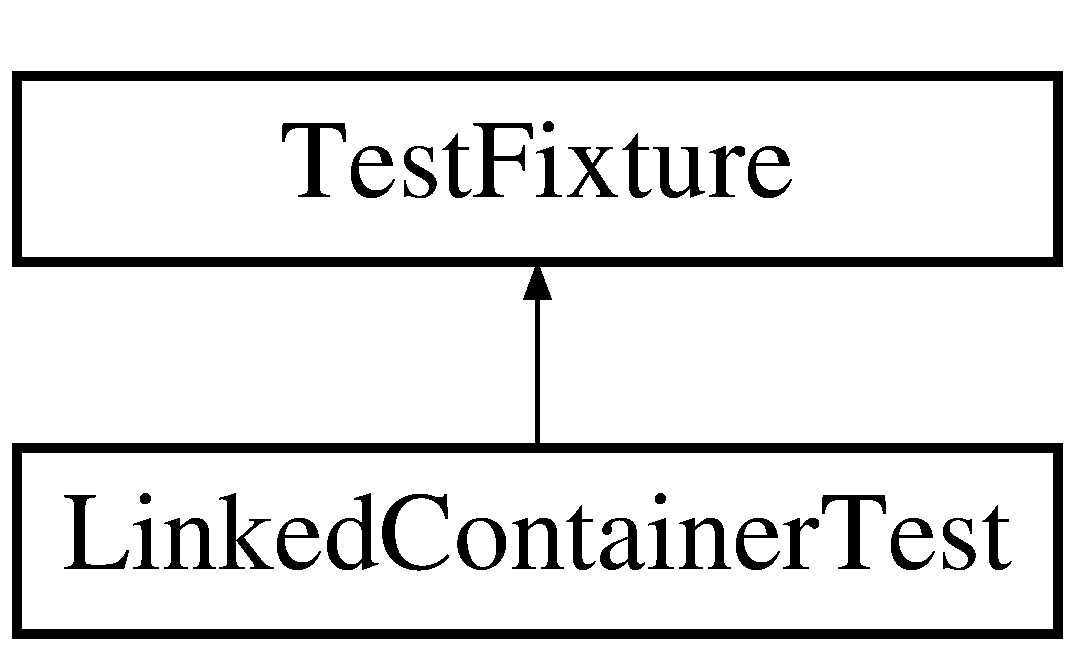
\includegraphics[height=2.000000cm]{classLinkedContainerTest}
\end{center}
\end{figure}
\subsection*{Public Member Functions}
\begin{DoxyCompactItemize}
\item 
void \hyperlink{classLinkedContainerTest_ad4c24c445d295e8ce6fd350e0d4d9fab}{set\+Up} ()
\item 
void \hyperlink{classLinkedContainerTest_a1afa7e2cd6633b6fef51fd403116baef}{add\+Particle\+Test} ()
\item 
void \hyperlink{classLinkedContainerTest_ab185ef32b0adc7be7b6de3baf007d8e2}{delete\+Particle\+Test} ()
\item 
void \hyperlink{classLinkedContainerTest_a7ce227622a1298dadc7027f9f8e4b850}{out\+Of\+Domain\+Test} ()
\item 
void \hyperlink{classLinkedContainerTest_a8a3c4f33b08c4c63acb05cd5b47fe2b8}{boundary\+Force\+Test} ()
\item 
void \hyperlink{classLinkedContainerTest_a3ea7a9a7335bc8d20c829bb7d0cd05ba}{boundary\+Test} ()
\item 
void \hyperlink{classLinkedContainerTest_adcf6642009e1818aad463c19f810b07c}{calculate\+F\+Test} ()
\item 
\hyperlink{classLinkedContainerTest_ab8351f042795c8508d360369e1900d3d}{Linked\+Container\+Test} ()
\item 
virtual \hyperlink{classLinkedContainerTest_a0d507051259d6878affd659cb771417e}{$\sim$\+Linked\+Container\+Test} ()
\end{DoxyCompactItemize}
\subsection*{Private Member Functions}
\begin{DoxyCompactItemize}
\item 
\hyperlink{classLinkedContainerTest_a00625077e5525884c6062662c9b01b5c}{C\+P\+P\+U\+N\+I\+T\+\_\+\+T\+E\+S\+T\+\_\+\+S\+U\+I\+TE} (\hyperlink{classLinkedContainerTest}{Linked\+Container\+Test})
\item 
\hyperlink{classLinkedContainerTest_abe995a0b3bd166156541fbaa1c2816d7}{C\+P\+P\+U\+N\+I\+T\+\_\+\+T\+E\+ST} (\hyperlink{classLinkedContainerTest_a1afa7e2cd6633b6fef51fd403116baef}{add\+Particle\+Test})
\item 
\hyperlink{classLinkedContainerTest_ab5611aeafd31118b2d3612cc3d978533}{C\+P\+P\+U\+N\+I\+T\+\_\+\+T\+E\+ST} (\hyperlink{classLinkedContainerTest_ab185ef32b0adc7be7b6de3baf007d8e2}{delete\+Particle\+Test})
\item 
\hyperlink{classLinkedContainerTest_a49d71f1e737194a59fb3882b5cc27ff4}{C\+P\+P\+U\+N\+I\+T\+\_\+\+T\+E\+ST} (\hyperlink{classLinkedContainerTest_a7ce227622a1298dadc7027f9f8e4b850}{out\+Of\+Domain\+Test})
\item 
\hyperlink{classLinkedContainerTest_aadca35c710fa6ce04410ebfa8f775b99}{C\+P\+P\+U\+N\+I\+T\+\_\+\+T\+E\+ST} (\hyperlink{classLinkedContainerTest_a8a3c4f33b08c4c63acb05cd5b47fe2b8}{boundary\+Force\+Test})
\item 
\hyperlink{classLinkedContainerTest_a4d719b9133e0396e8edbccd7dfd3d696}{C\+P\+P\+U\+N\+I\+T\+\_\+\+T\+E\+ST} (\hyperlink{classLinkedContainerTest_a3ea7a9a7335bc8d20c829bb7d0cd05ba}{boundary\+Test})
\item 
\hyperlink{classLinkedContainerTest_a2679aa59704d6af4eeafd77065f83563}{C\+P\+P\+U\+N\+I\+T\+\_\+\+T\+E\+ST} (\hyperlink{classLinkedContainerTest_adcf6642009e1818aad463c19f810b07c}{calculate\+F\+Test})
\item 
\hyperlink{classLinkedContainerTest_a73506489a7532733d8dba14efa8bc407}{C\+P\+P\+U\+N\+I\+T\+\_\+\+T\+E\+S\+T\+\_\+\+S\+U\+I\+T\+E\+\_\+\+E\+ND} ()
\end{DoxyCompactItemize}


\subsection{Detailed Description}
Test\+Suite for Linked\+Container. 

\subsection{Constructor \& Destructor Documentation}
\index{Linked\+Container\+Test@{Linked\+Container\+Test}!Linked\+Container\+Test@{Linked\+Container\+Test}}
\index{Linked\+Container\+Test@{Linked\+Container\+Test}!Linked\+Container\+Test@{Linked\+Container\+Test}}
\subsubsection[{\texorpdfstring{Linked\+Container\+Test()}{LinkedContainerTest()}}]{\setlength{\rightskip}{0pt plus 5cm}Linked\+Container\+Test\+::\+Linked\+Container\+Test (
\begin{DoxyParamCaption}
{}
\end{DoxyParamCaption}
)}\hypertarget{classLinkedContainerTest_ab8351f042795c8508d360369e1900d3d}{}\label{classLinkedContainerTest_ab8351f042795c8508d360369e1900d3d}
\index{Linked\+Container\+Test@{Linked\+Container\+Test}!````~Linked\+Container\+Test@{$\sim$\+Linked\+Container\+Test}}
\index{````~Linked\+Container\+Test@{$\sim$\+Linked\+Container\+Test}!Linked\+Container\+Test@{Linked\+Container\+Test}}
\subsubsection[{\texorpdfstring{$\sim$\+Linked\+Container\+Test()}{~LinkedContainerTest()}}]{\setlength{\rightskip}{0pt plus 5cm}Linked\+Container\+Test\+::$\sim$\+Linked\+Container\+Test (
\begin{DoxyParamCaption}
{}
\end{DoxyParamCaption}
)\hspace{0.3cm}{\ttfamily [virtual]}}\hypertarget{classLinkedContainerTest_a0d507051259d6878affd659cb771417e}{}\label{classLinkedContainerTest_a0d507051259d6878affd659cb771417e}


\subsection{Member Function Documentation}
\index{Linked\+Container\+Test@{Linked\+Container\+Test}!add\+Particle\+Test@{add\+Particle\+Test}}
\index{add\+Particle\+Test@{add\+Particle\+Test}!Linked\+Container\+Test@{Linked\+Container\+Test}}
\subsubsection[{\texorpdfstring{add\+Particle\+Test()}{addParticleTest()}}]{\setlength{\rightskip}{0pt plus 5cm}void Linked\+Container\+Test\+::add\+Particle\+Test (
\begin{DoxyParamCaption}
{}
\end{DoxyParamCaption}
)}\hypertarget{classLinkedContainerTest_a1afa7e2cd6633b6fef51fd403116baef}{}\label{classLinkedContainerTest_a1afa7e2cd6633b6fef51fd403116baef}
Tests if particles are added, but copies are ignored \index{Linked\+Container\+Test@{Linked\+Container\+Test}!boundary\+Force\+Test@{boundary\+Force\+Test}}
\index{boundary\+Force\+Test@{boundary\+Force\+Test}!Linked\+Container\+Test@{Linked\+Container\+Test}}
\subsubsection[{\texorpdfstring{boundary\+Force\+Test()}{boundaryForceTest()}}]{\setlength{\rightskip}{0pt plus 5cm}void Linked\+Container\+Test\+::boundary\+Force\+Test (
\begin{DoxyParamCaption}
{}
\end{DoxyParamCaption}
)}\hypertarget{classLinkedContainerTest_a8a3c4f33b08c4c63acb05cd5b47fe2b8}{}\label{classLinkedContainerTest_a8a3c4f33b08c4c63acb05cd5b47fe2b8}
Tests if particles are deleted if out of domain \index{Linked\+Container\+Test@{Linked\+Container\+Test}!boundary\+Test@{boundary\+Test}}
\index{boundary\+Test@{boundary\+Test}!Linked\+Container\+Test@{Linked\+Container\+Test}}
\subsubsection[{\texorpdfstring{boundary\+Test()}{boundaryTest()}}]{\setlength{\rightskip}{0pt plus 5cm}void Linked\+Container\+Test\+::boundary\+Test (
\begin{DoxyParamCaption}
{}
\end{DoxyParamCaption}
)}\hypertarget{classLinkedContainerTest_a3ea7a9a7335bc8d20c829bb7d0cd05ba}{}\label{classLinkedContainerTest_a3ea7a9a7335bc8d20c829bb7d0cd05ba}
Tests if particles are recognized in the boundary \index{Linked\+Container\+Test@{Linked\+Container\+Test}!calculate\+F\+Test@{calculate\+F\+Test}}
\index{calculate\+F\+Test@{calculate\+F\+Test}!Linked\+Container\+Test@{Linked\+Container\+Test}}
\subsubsection[{\texorpdfstring{calculate\+F\+Test()}{calculateFTest()}}]{\setlength{\rightskip}{0pt plus 5cm}void Linked\+Container\+Test\+::calculate\+F\+Test (
\begin{DoxyParamCaption}
{}
\end{DoxyParamCaption}
)}\hypertarget{classLinkedContainerTest_adcf6642009e1818aad463c19f810b07c}{}\label{classLinkedContainerTest_adcf6642009e1818aad463c19f810b07c}
Test if the forces are calculated correctly \index{Linked\+Container\+Test@{Linked\+Container\+Test}!C\+P\+P\+U\+N\+I\+T\+\_\+\+T\+E\+ST@{C\+P\+P\+U\+N\+I\+T\+\_\+\+T\+E\+ST}}
\index{C\+P\+P\+U\+N\+I\+T\+\_\+\+T\+E\+ST@{C\+P\+P\+U\+N\+I\+T\+\_\+\+T\+E\+ST}!Linked\+Container\+Test@{Linked\+Container\+Test}}
\subsubsection[{\texorpdfstring{C\+P\+P\+U\+N\+I\+T\+\_\+\+T\+E\+S\+T(add\+Particle\+Test)}{CPPUNIT_TEST(addParticleTest)}}]{\setlength{\rightskip}{0pt plus 5cm}Linked\+Container\+Test\+::\+C\+P\+P\+U\+N\+I\+T\+\_\+\+T\+E\+ST (
\begin{DoxyParamCaption}
\item[{{\bf add\+Particle\+Test}}]{}
\end{DoxyParamCaption}
)\hspace{0.3cm}{\ttfamily [private]}}\hypertarget{classLinkedContainerTest_abe995a0b3bd166156541fbaa1c2816d7}{}\label{classLinkedContainerTest_abe995a0b3bd166156541fbaa1c2816d7}
\index{Linked\+Container\+Test@{Linked\+Container\+Test}!C\+P\+P\+U\+N\+I\+T\+\_\+\+T\+E\+ST@{C\+P\+P\+U\+N\+I\+T\+\_\+\+T\+E\+ST}}
\index{C\+P\+P\+U\+N\+I\+T\+\_\+\+T\+E\+ST@{C\+P\+P\+U\+N\+I\+T\+\_\+\+T\+E\+ST}!Linked\+Container\+Test@{Linked\+Container\+Test}}
\subsubsection[{\texorpdfstring{C\+P\+P\+U\+N\+I\+T\+\_\+\+T\+E\+S\+T(delete\+Particle\+Test)}{CPPUNIT_TEST(deleteParticleTest)}}]{\setlength{\rightskip}{0pt plus 5cm}Linked\+Container\+Test\+::\+C\+P\+P\+U\+N\+I\+T\+\_\+\+T\+E\+ST (
\begin{DoxyParamCaption}
\item[{{\bf delete\+Particle\+Test}}]{}
\end{DoxyParamCaption}
)\hspace{0.3cm}{\ttfamily [private]}}\hypertarget{classLinkedContainerTest_ab5611aeafd31118b2d3612cc3d978533}{}\label{classLinkedContainerTest_ab5611aeafd31118b2d3612cc3d978533}
\index{Linked\+Container\+Test@{Linked\+Container\+Test}!C\+P\+P\+U\+N\+I\+T\+\_\+\+T\+E\+ST@{C\+P\+P\+U\+N\+I\+T\+\_\+\+T\+E\+ST}}
\index{C\+P\+P\+U\+N\+I\+T\+\_\+\+T\+E\+ST@{C\+P\+P\+U\+N\+I\+T\+\_\+\+T\+E\+ST}!Linked\+Container\+Test@{Linked\+Container\+Test}}
\subsubsection[{\texorpdfstring{C\+P\+P\+U\+N\+I\+T\+\_\+\+T\+E\+S\+T(out\+Of\+Domain\+Test)}{CPPUNIT_TEST(outOfDomainTest)}}]{\setlength{\rightskip}{0pt plus 5cm}Linked\+Container\+Test\+::\+C\+P\+P\+U\+N\+I\+T\+\_\+\+T\+E\+ST (
\begin{DoxyParamCaption}
\item[{{\bf out\+Of\+Domain\+Test}}]{}
\end{DoxyParamCaption}
)\hspace{0.3cm}{\ttfamily [private]}}\hypertarget{classLinkedContainerTest_a49d71f1e737194a59fb3882b5cc27ff4}{}\label{classLinkedContainerTest_a49d71f1e737194a59fb3882b5cc27ff4}
\index{Linked\+Container\+Test@{Linked\+Container\+Test}!C\+P\+P\+U\+N\+I\+T\+\_\+\+T\+E\+ST@{C\+P\+P\+U\+N\+I\+T\+\_\+\+T\+E\+ST}}
\index{C\+P\+P\+U\+N\+I\+T\+\_\+\+T\+E\+ST@{C\+P\+P\+U\+N\+I\+T\+\_\+\+T\+E\+ST}!Linked\+Container\+Test@{Linked\+Container\+Test}}
\subsubsection[{\texorpdfstring{C\+P\+P\+U\+N\+I\+T\+\_\+\+T\+E\+S\+T(boundary\+Force\+Test)}{CPPUNIT_TEST(boundaryForceTest)}}]{\setlength{\rightskip}{0pt plus 5cm}Linked\+Container\+Test\+::\+C\+P\+P\+U\+N\+I\+T\+\_\+\+T\+E\+ST (
\begin{DoxyParamCaption}
\item[{{\bf boundary\+Force\+Test}}]{}
\end{DoxyParamCaption}
)\hspace{0.3cm}{\ttfamily [private]}}\hypertarget{classLinkedContainerTest_aadca35c710fa6ce04410ebfa8f775b99}{}\label{classLinkedContainerTest_aadca35c710fa6ce04410ebfa8f775b99}
\index{Linked\+Container\+Test@{Linked\+Container\+Test}!C\+P\+P\+U\+N\+I\+T\+\_\+\+T\+E\+ST@{C\+P\+P\+U\+N\+I\+T\+\_\+\+T\+E\+ST}}
\index{C\+P\+P\+U\+N\+I\+T\+\_\+\+T\+E\+ST@{C\+P\+P\+U\+N\+I\+T\+\_\+\+T\+E\+ST}!Linked\+Container\+Test@{Linked\+Container\+Test}}
\subsubsection[{\texorpdfstring{C\+P\+P\+U\+N\+I\+T\+\_\+\+T\+E\+S\+T(boundary\+Test)}{CPPUNIT_TEST(boundaryTest)}}]{\setlength{\rightskip}{0pt plus 5cm}Linked\+Container\+Test\+::\+C\+P\+P\+U\+N\+I\+T\+\_\+\+T\+E\+ST (
\begin{DoxyParamCaption}
\item[{{\bf boundary\+Test}}]{}
\end{DoxyParamCaption}
)\hspace{0.3cm}{\ttfamily [private]}}\hypertarget{classLinkedContainerTest_a4d719b9133e0396e8edbccd7dfd3d696}{}\label{classLinkedContainerTest_a4d719b9133e0396e8edbccd7dfd3d696}
\index{Linked\+Container\+Test@{Linked\+Container\+Test}!C\+P\+P\+U\+N\+I\+T\+\_\+\+T\+E\+ST@{C\+P\+P\+U\+N\+I\+T\+\_\+\+T\+E\+ST}}
\index{C\+P\+P\+U\+N\+I\+T\+\_\+\+T\+E\+ST@{C\+P\+P\+U\+N\+I\+T\+\_\+\+T\+E\+ST}!Linked\+Container\+Test@{Linked\+Container\+Test}}
\subsubsection[{\texorpdfstring{C\+P\+P\+U\+N\+I\+T\+\_\+\+T\+E\+S\+T(calculate\+F\+Test)}{CPPUNIT_TEST(calculateFTest)}}]{\setlength{\rightskip}{0pt plus 5cm}Linked\+Container\+Test\+::\+C\+P\+P\+U\+N\+I\+T\+\_\+\+T\+E\+ST (
\begin{DoxyParamCaption}
\item[{{\bf calculate\+F\+Test}}]{}
\end{DoxyParamCaption}
)\hspace{0.3cm}{\ttfamily [private]}}\hypertarget{classLinkedContainerTest_a2679aa59704d6af4eeafd77065f83563}{}\label{classLinkedContainerTest_a2679aa59704d6af4eeafd77065f83563}
\index{Linked\+Container\+Test@{Linked\+Container\+Test}!C\+P\+P\+U\+N\+I\+T\+\_\+\+T\+E\+S\+T\+\_\+\+S\+U\+I\+TE@{C\+P\+P\+U\+N\+I\+T\+\_\+\+T\+E\+S\+T\+\_\+\+S\+U\+I\+TE}}
\index{C\+P\+P\+U\+N\+I\+T\+\_\+\+T\+E\+S\+T\+\_\+\+S\+U\+I\+TE@{C\+P\+P\+U\+N\+I\+T\+\_\+\+T\+E\+S\+T\+\_\+\+S\+U\+I\+TE}!Linked\+Container\+Test@{Linked\+Container\+Test}}
\subsubsection[{\texorpdfstring{C\+P\+P\+U\+N\+I\+T\+\_\+\+T\+E\+S\+T\+\_\+\+S\+U\+I\+T\+E(\+Linked\+Container\+Test)}{CPPUNIT_TEST_SUITE(LinkedContainerTest)}}]{\setlength{\rightskip}{0pt plus 5cm}Linked\+Container\+Test\+::\+C\+P\+P\+U\+N\+I\+T\+\_\+\+T\+E\+S\+T\+\_\+\+S\+U\+I\+TE (
\begin{DoxyParamCaption}
\item[{{\bf Linked\+Container\+Test}}]{}
\end{DoxyParamCaption}
)\hspace{0.3cm}{\ttfamily [private]}}\hypertarget{classLinkedContainerTest_a00625077e5525884c6062662c9b01b5c}{}\label{classLinkedContainerTest_a00625077e5525884c6062662c9b01b5c}
\index{Linked\+Container\+Test@{Linked\+Container\+Test}!C\+P\+P\+U\+N\+I\+T\+\_\+\+T\+E\+S\+T\+\_\+\+S\+U\+I\+T\+E\+\_\+\+E\+ND@{C\+P\+P\+U\+N\+I\+T\+\_\+\+T\+E\+S\+T\+\_\+\+S\+U\+I\+T\+E\+\_\+\+E\+ND}}
\index{C\+P\+P\+U\+N\+I\+T\+\_\+\+T\+E\+S\+T\+\_\+\+S\+U\+I\+T\+E\+\_\+\+E\+ND@{C\+P\+P\+U\+N\+I\+T\+\_\+\+T\+E\+S\+T\+\_\+\+S\+U\+I\+T\+E\+\_\+\+E\+ND}!Linked\+Container\+Test@{Linked\+Container\+Test}}
\subsubsection[{\texorpdfstring{C\+P\+P\+U\+N\+I\+T\+\_\+\+T\+E\+S\+T\+\_\+\+S\+U\+I\+T\+E\+\_\+\+E\+N\+D()}{CPPUNIT_TEST_SUITE_END()}}]{\setlength{\rightskip}{0pt plus 5cm}Linked\+Container\+Test\+::\+C\+P\+P\+U\+N\+I\+T\+\_\+\+T\+E\+S\+T\+\_\+\+S\+U\+I\+T\+E\+\_\+\+E\+ND (
\begin{DoxyParamCaption}
{}
\end{DoxyParamCaption}
)\hspace{0.3cm}{\ttfamily [private]}}\hypertarget{classLinkedContainerTest_a73506489a7532733d8dba14efa8bc407}{}\label{classLinkedContainerTest_a73506489a7532733d8dba14efa8bc407}
\index{Linked\+Container\+Test@{Linked\+Container\+Test}!delete\+Particle\+Test@{delete\+Particle\+Test}}
\index{delete\+Particle\+Test@{delete\+Particle\+Test}!Linked\+Container\+Test@{Linked\+Container\+Test}}
\subsubsection[{\texorpdfstring{delete\+Particle\+Test()}{deleteParticleTest()}}]{\setlength{\rightskip}{0pt plus 5cm}void Linked\+Container\+Test\+::delete\+Particle\+Test (
\begin{DoxyParamCaption}
{}
\end{DoxyParamCaption}
)}\hypertarget{classLinkedContainerTest_ab185ef32b0adc7be7b6de3baf007d8e2}{}\label{classLinkedContainerTest_ab185ef32b0adc7be7b6de3baf007d8e2}
Tests if particles are deleted if in container \index{Linked\+Container\+Test@{Linked\+Container\+Test}!out\+Of\+Domain\+Test@{out\+Of\+Domain\+Test}}
\index{out\+Of\+Domain\+Test@{out\+Of\+Domain\+Test}!Linked\+Container\+Test@{Linked\+Container\+Test}}
\subsubsection[{\texorpdfstring{out\+Of\+Domain\+Test()}{outOfDomainTest()}}]{\setlength{\rightskip}{0pt plus 5cm}void Linked\+Container\+Test\+::out\+Of\+Domain\+Test (
\begin{DoxyParamCaption}
{}
\end{DoxyParamCaption}
)}\hypertarget{classLinkedContainerTest_a7ce227622a1298dadc7027f9f8e4b850}{}\label{classLinkedContainerTest_a7ce227622a1298dadc7027f9f8e4b850}
Tests if particles are deleted if out of domain \index{Linked\+Container\+Test@{Linked\+Container\+Test}!set\+Up@{set\+Up}}
\index{set\+Up@{set\+Up}!Linked\+Container\+Test@{Linked\+Container\+Test}}
\subsubsection[{\texorpdfstring{set\+Up()}{setUp()}}]{\setlength{\rightskip}{0pt plus 5cm}void Linked\+Container\+Test\+::set\+Up (
\begin{DoxyParamCaption}
{}
\end{DoxyParamCaption}
)}\hypertarget{classLinkedContainerTest_ad4c24c445d295e8ce6fd350e0d4d9fab}{}\label{classLinkedContainerTest_ad4c24c445d295e8ce6fd350e0d4d9fab}


The documentation for this class was generated from the following files\+:\begin{DoxyCompactItemize}
\item 
src/tests/\hyperlink{LinkedContainerTest_8h}{Linked\+Container\+Test.\+h}\item 
src/tests/\hyperlink{LinkedContainerTest_8cpp}{Linked\+Container\+Test.\+cpp}\end{DoxyCompactItemize}

\hypertarget{classmembrane__t}{}\section{membrane\+\_\+t Class Reference}
\label{classmembrane__t}\index{membrane\+\_\+t@{membrane\+\_\+t}}


{\ttfamily \#include $<$particle\+\_\+input.\+h$>$}

Inheritance diagram for membrane\+\_\+t\+:\begin{figure}[H]
\begin{center}
\leavevmode
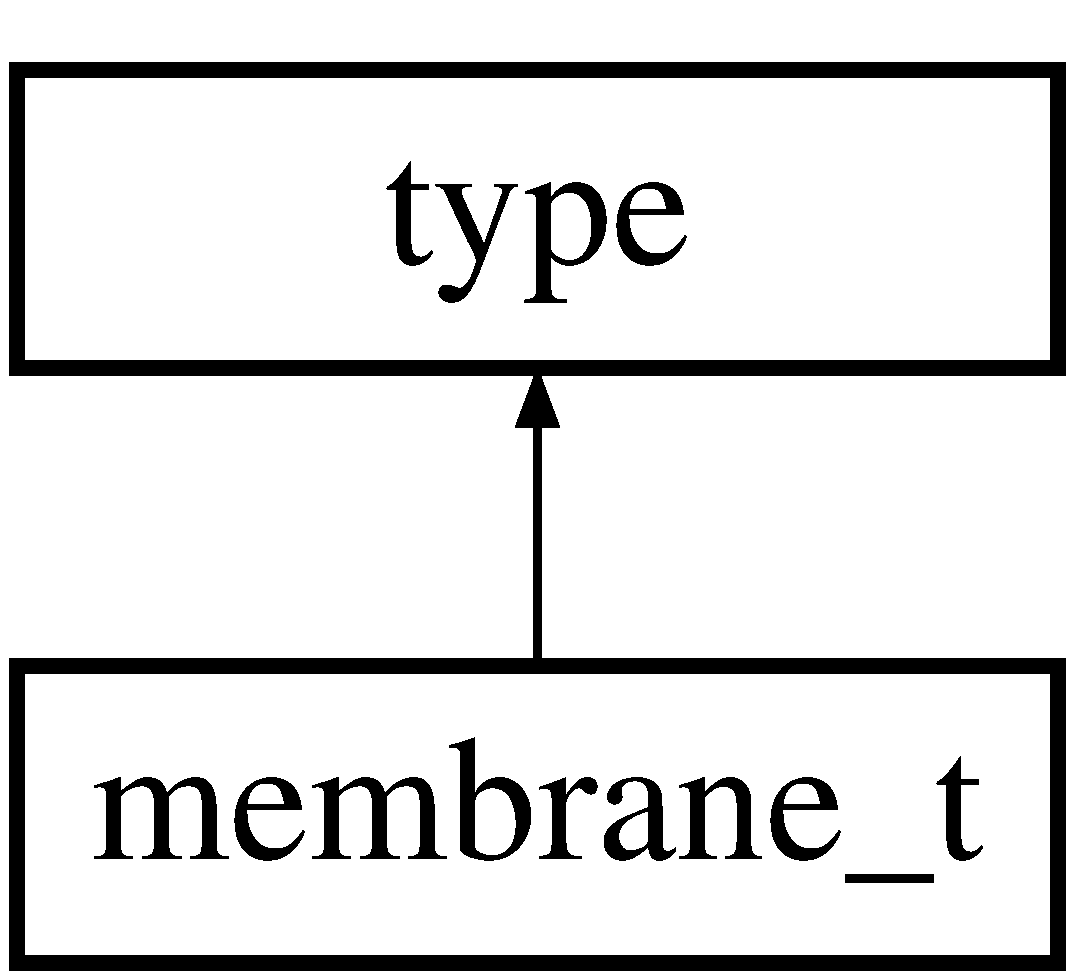
\includegraphics[height=2.000000cm]{classmembrane__t}
\end{center}
\end{figure}
\subsection*{Public Types}
\begin{DoxyCompactItemize}
\item 
typedef \+::\hyperlink{namespacexml__schema_aac2d3d3483d3a20e8d96d2e8e5b3a470}{xml\+\_\+schema\+::double\+\_\+} \hyperlink{classmembrane__t_a9e55619d3d02a55660849deaa0ca4338}{stiffness\+\_\+type}
\item 
typedef \+::xsd\+::cxx\+::tree\+::traits$<$ \hyperlink{classmembrane__t_a9e55619d3d02a55660849deaa0ca4338}{stiffness\+\_\+type}, char,\+::xsd\+::cxx\+::tree\+::schema\+\_\+type\+::double\+\_\+ $>$ \hyperlink{classmembrane__t_a90e2a51b2f18f88127057a926cce542a}{stiffness\+\_\+traits}
\item 
typedef \+::\hyperlink{namespacexml__schema_aac2d3d3483d3a20e8d96d2e8e5b3a470}{xml\+\_\+schema\+::double\+\_\+} \hyperlink{classmembrane__t_ab1e0c179101c4b2916059925d73468ff}{r\+\_\+zero\+\_\+type}
\item 
typedef \+::xsd\+::cxx\+::tree\+::traits$<$ \hyperlink{classmembrane__t_ab1e0c179101c4b2916059925d73468ff}{r\+\_\+zero\+\_\+type}, char,\+::xsd\+::cxx\+::tree\+::schema\+\_\+type\+::double\+\_\+ $>$ \hyperlink{classmembrane__t_aebe5eb10f95c19f95c3946d3bbb9adb8}{r\+\_\+zero\+\_\+traits}
\item 
typedef \+::\hyperlink{classvector__t}{vector\+\_\+t} \hyperlink{classmembrane__t_ab4d91a3ba331c16adbf69418f876f849}{force\+\_\+type}
\item 
typedef \+::xsd\+::cxx\+::tree\+::optional$<$ \hyperlink{classmembrane__t_ab4d91a3ba331c16adbf69418f876f849}{force\+\_\+type} $>$ \hyperlink{classmembrane__t_a558422b23faa72b3e4cbc060f9ff8ea3}{force\+\_\+optional}
\item 
typedef \+::xsd\+::cxx\+::tree\+::traits$<$ \hyperlink{classmembrane__t_ab4d91a3ba331c16adbf69418f876f849}{force\+\_\+type}, char $>$ \hyperlink{classmembrane__t_a2b6b177c77d6eddf152913810d47f7f7}{force\+\_\+traits}
\item 
typedef \+::\hyperlink{namespacexml__schema_aac2d3d3483d3a20e8d96d2e8e5b3a470}{xml\+\_\+schema\+::double\+\_\+} \hyperlink{classmembrane__t_a9c464d55e3d8162b6bb521d9dd6d761d}{t\+\_\+end\+\_\+force\+\_\+type}
\item 
typedef \+::xsd\+::cxx\+::tree\+::optional$<$ \hyperlink{classmembrane__t_a9c464d55e3d8162b6bb521d9dd6d761d}{t\+\_\+end\+\_\+force\+\_\+type} $>$ \hyperlink{classmembrane__t_a7725d61ae95e124d402a8d9db7a08376}{t\+\_\+end\+\_\+force\+\_\+optional}
\item 
typedef \+::xsd\+::cxx\+::tree\+::traits$<$ \hyperlink{classmembrane__t_a9c464d55e3d8162b6bb521d9dd6d761d}{t\+\_\+end\+\_\+force\+\_\+type}, char,\+::xsd\+::cxx\+::tree\+::schema\+\_\+type\+::double\+\_\+ $>$ \hyperlink{classmembrane__t_a6e52d2cbbfa0781d7ce3aec95ce1a7ab}{t\+\_\+end\+\_\+force\+\_\+traits}
\item 
typedef \+::\hyperlink{classint__vector__t}{int\+\_\+vector\+\_\+t} \hyperlink{classmembrane__t_a8866c2084ca9b88e98340080008777e5}{coord\+\_\+force\+\_\+type}
\item 
typedef \+::xsd\+::cxx\+::tree\+::sequence$<$ \hyperlink{classmembrane__t_a8866c2084ca9b88e98340080008777e5}{coord\+\_\+force\+\_\+type} $>$ \hyperlink{classmembrane__t_a2825c9df8bf471f2c5053a826cf6fcb0}{coord\+\_\+force\+\_\+sequence}
\item 
typedef coord\+\_\+force\+\_\+sequence\+::iterator \hyperlink{classmembrane__t_adb487c2f17c0b6197225dbc0beb9990c}{coord\+\_\+force\+\_\+iterator}
\item 
typedef coord\+\_\+force\+\_\+sequence\+::const\+\_\+iterator \hyperlink{classmembrane__t_a558f9ccc1036a61e199e93fe08646cec}{coord\+\_\+force\+\_\+const\+\_\+iterator}
\item 
typedef \+::xsd\+::cxx\+::tree\+::traits$<$ \hyperlink{classmembrane__t_a8866c2084ca9b88e98340080008777e5}{coord\+\_\+force\+\_\+type}, char $>$ \hyperlink{classmembrane__t_a5edce7be5d85743cf318cbc01750134e}{coord\+\_\+force\+\_\+traits}
\item 
typedef \+::\hyperlink{classvector__t}{vector\+\_\+t} \hyperlink{classmembrane__t_a0841f5bafc269d612a4b6fefcce1d73f}{coord\+\_\+type}
\item 
typedef \+::xsd\+::cxx\+::tree\+::traits$<$ \hyperlink{classmembrane__t_a0841f5bafc269d612a4b6fefcce1d73f}{coord\+\_\+type}, char $>$ \hyperlink{classmembrane__t_ad5ae6696a73759a2dacbed6d33371fbf}{coord\+\_\+traits}
\item 
typedef \+::\hyperlink{classint__vector__t}{int\+\_\+vector\+\_\+t} \hyperlink{classmembrane__t_afdd0310501689ebab285ec39821c5b76}{dimension\+\_\+type}
\item 
typedef \+::xsd\+::cxx\+::tree\+::traits$<$ \hyperlink{classmembrane__t_afdd0310501689ebab285ec39821c5b76}{dimension\+\_\+type}, char $>$ \hyperlink{classmembrane__t_aa3e274a54801b84c5dae45b44bfe86a0}{dimension\+\_\+traits}
\item 
typedef \+::\hyperlink{namespacexml__schema_ad7e04ab17bba0b3fdde43fb79ef6ed87}{xml\+\_\+schema\+::float\+\_\+} \hyperlink{classmembrane__t_a259dfb54e3d4a66cdd72b5b0831f4188}{mesh\+\_\+type}
\item 
typedef \+::xsd\+::cxx\+::tree\+::traits$<$ \hyperlink{classmembrane__t_a259dfb54e3d4a66cdd72b5b0831f4188}{mesh\+\_\+type}, char $>$ \hyperlink{classmembrane__t_a6b611201cacd05e394dc2d6750a33ff9}{mesh\+\_\+traits}
\item 
typedef \+::\hyperlink{classvector__t}{vector\+\_\+t} \hyperlink{classmembrane__t_a41bad26c4626a8ceac158b3817306c62}{velocity\+\_\+type}
\item 
typedef \+::xsd\+::cxx\+::tree\+::traits$<$ \hyperlink{classmembrane__t_a41bad26c4626a8ceac158b3817306c62}{velocity\+\_\+type}, char $>$ \hyperlink{classmembrane__t_aa9cbbb0853e5efae969241a0bfe951b6}{velocity\+\_\+traits}
\item 
typedef \+::\hyperlink{namespacexml__schema_acfa24ac68e1a188e7f44c36f7a158bf4}{xml\+\_\+schema\+::int\+\_\+} \hyperlink{classmembrane__t_a13eb0ee51a5a6018151503690e28e2fb}{type\+\_\+type}
\item 
typedef \+::xsd\+::cxx\+::tree\+::traits$<$ \hyperlink{classmembrane__t_a13eb0ee51a5a6018151503690e28e2fb}{type\+\_\+type}, char $>$ \hyperlink{classmembrane__t_ac54c3884b125d2a162ce454e82f4da69}{type\+\_\+traits}
\end{DoxyCompactItemize}
\subsection*{Public Member Functions}
\begin{DoxyCompactItemize}
\item 
const \hyperlink{classmembrane__t_a9e55619d3d02a55660849deaa0ca4338}{stiffness\+\_\+type} \& \hyperlink{classmembrane__t_a798d5aac4ed960e2ad95d675c89e27a2}{stiffness} () const 
\item 
\hyperlink{classmembrane__t_a9e55619d3d02a55660849deaa0ca4338}{stiffness\+\_\+type} \& \hyperlink{classmembrane__t_a3f9153cf9ac73898479bf5722b6531ef}{stiffness} ()
\item 
void \hyperlink{classmembrane__t_ae30350a7d27308cd43ebdef96e3a159c}{stiffness} (const \hyperlink{classmembrane__t_a9e55619d3d02a55660849deaa0ca4338}{stiffness\+\_\+type} \&x)
\item 
const \hyperlink{classmembrane__t_ab1e0c179101c4b2916059925d73468ff}{r\+\_\+zero\+\_\+type} \& \hyperlink{classmembrane__t_aa2e292d4f0aa5c09a75596c85c373ec3}{r\+\_\+zero} () const 
\item 
\hyperlink{classmembrane__t_ab1e0c179101c4b2916059925d73468ff}{r\+\_\+zero\+\_\+type} \& \hyperlink{classmembrane__t_a859cf64e389832eada24f2776501e879}{r\+\_\+zero} ()
\item 
void \hyperlink{classmembrane__t_aca35bd2dc12a569910c52e9b4b5a4b53}{r\+\_\+zero} (const \hyperlink{classmembrane__t_ab1e0c179101c4b2916059925d73468ff}{r\+\_\+zero\+\_\+type} \&x)
\item 
const \hyperlink{classmembrane__t_a558422b23faa72b3e4cbc060f9ff8ea3}{force\+\_\+optional} \& \hyperlink{classmembrane__t_a0746bbae2169a7afca45b7e2d10db24d}{force} () const 
\item 
\hyperlink{classmembrane__t_a558422b23faa72b3e4cbc060f9ff8ea3}{force\+\_\+optional} \& \hyperlink{classmembrane__t_a6f0d435bd62b2b8b436589fcb5c1b7fb}{force} ()
\item 
void \hyperlink{classmembrane__t_ac6e5247264e0fb528a1e804b66782ff8}{force} (const \hyperlink{classmembrane__t_ab4d91a3ba331c16adbf69418f876f849}{force\+\_\+type} \&x)
\item 
void \hyperlink{classmembrane__t_aae94af1cb55045583a9fa0d471c64cc4}{force} (const \hyperlink{classmembrane__t_a558422b23faa72b3e4cbc060f9ff8ea3}{force\+\_\+optional} \&x)
\item 
void \hyperlink{classmembrane__t_a6bc29b3af98820be7dd1187c0c736e4d}{force} (\+::std\+::unique\+\_\+ptr$<$ \hyperlink{classmembrane__t_ab4d91a3ba331c16adbf69418f876f849}{force\+\_\+type} $>$ p)
\item 
const \hyperlink{classmembrane__t_a7725d61ae95e124d402a8d9db7a08376}{t\+\_\+end\+\_\+force\+\_\+optional} \& \hyperlink{classmembrane__t_ad3d07daa7aaa84cac85479dea684a281}{t\+\_\+end\+\_\+force} () const 
\item 
\hyperlink{classmembrane__t_a7725d61ae95e124d402a8d9db7a08376}{t\+\_\+end\+\_\+force\+\_\+optional} \& \hyperlink{classmembrane__t_a937765794f5b3841397d876dfe433e45}{t\+\_\+end\+\_\+force} ()
\item 
void \hyperlink{classmembrane__t_a9a35db0433da0b52cbe1c6a7d71cd064}{t\+\_\+end\+\_\+force} (const \hyperlink{classmembrane__t_a9c464d55e3d8162b6bb521d9dd6d761d}{t\+\_\+end\+\_\+force\+\_\+type} \&x)
\item 
void \hyperlink{classmembrane__t_aaec36e48218d3eb6503c623038621f06}{t\+\_\+end\+\_\+force} (const \hyperlink{classmembrane__t_a7725d61ae95e124d402a8d9db7a08376}{t\+\_\+end\+\_\+force\+\_\+optional} \&x)
\item 
const \hyperlink{classmembrane__t_a2825c9df8bf471f2c5053a826cf6fcb0}{coord\+\_\+force\+\_\+sequence} \& \hyperlink{classmembrane__t_a28c155d2af14f466f6cadd4ad2be09b6}{coord\+\_\+force} () const 
\item 
\hyperlink{classmembrane__t_a2825c9df8bf471f2c5053a826cf6fcb0}{coord\+\_\+force\+\_\+sequence} \& \hyperlink{classmembrane__t_a5ecc300d611f56ad4c4aef1963a891fd}{coord\+\_\+force} ()
\item 
void \hyperlink{classmembrane__t_a1500c28ae9c1483bfcfa922b1cd1f895}{coord\+\_\+force} (const \hyperlink{classmembrane__t_a2825c9df8bf471f2c5053a826cf6fcb0}{coord\+\_\+force\+\_\+sequence} \&s)
\item 
const \hyperlink{classmembrane__t_a0841f5bafc269d612a4b6fefcce1d73f}{coord\+\_\+type} \& \hyperlink{classmembrane__t_ae1af37f1ad61d584c7c937f714eb2143}{coord} () const 
\item 
\hyperlink{classmembrane__t_a0841f5bafc269d612a4b6fefcce1d73f}{coord\+\_\+type} \& \hyperlink{classmembrane__t_a3f3bba04ce2e3ef4377c22438aceffa3}{coord} ()
\item 
void \hyperlink{classmembrane__t_a371848cd38b967da540276a508738d14}{coord} (const \hyperlink{classmembrane__t_a0841f5bafc269d612a4b6fefcce1d73f}{coord\+\_\+type} \&x)
\item 
void \hyperlink{classmembrane__t_a82711d526f1a5be0f38d0158adb1f977}{coord} (\+::std\+::unique\+\_\+ptr$<$ \hyperlink{classmembrane__t_a0841f5bafc269d612a4b6fefcce1d73f}{coord\+\_\+type} $>$ p)
\item 
const \hyperlink{classmembrane__t_afdd0310501689ebab285ec39821c5b76}{dimension\+\_\+type} \& \hyperlink{classmembrane__t_a7e32345fb2d04840937a5943ac7a7070}{dimension} () const 
\item 
\hyperlink{classmembrane__t_afdd0310501689ebab285ec39821c5b76}{dimension\+\_\+type} \& \hyperlink{classmembrane__t_a279eb1c9154bcfa88346391dee4d2cc8}{dimension} ()
\item 
void \hyperlink{classmembrane__t_aac3e97b8eab6473296ad03b6ee871e9a}{dimension} (const \hyperlink{classmembrane__t_afdd0310501689ebab285ec39821c5b76}{dimension\+\_\+type} \&x)
\item 
void \hyperlink{classmembrane__t_a63a682a09f95a84f2e068c77e031b190}{dimension} (\+::std\+::unique\+\_\+ptr$<$ \hyperlink{classmembrane__t_afdd0310501689ebab285ec39821c5b76}{dimension\+\_\+type} $>$ p)
\item 
const \hyperlink{classmembrane__t_a259dfb54e3d4a66cdd72b5b0831f4188}{mesh\+\_\+type} \& \hyperlink{classmembrane__t_afdf7f5ae5b5b1057e7c0cda79b33fbde}{mesh} () const 
\item 
\hyperlink{classmembrane__t_a259dfb54e3d4a66cdd72b5b0831f4188}{mesh\+\_\+type} \& \hyperlink{classmembrane__t_a9f1158a643e80ed0e813bd480fc8036a}{mesh} ()
\item 
void \hyperlink{classmembrane__t_a3e9a65ce4a1891a7e3abd889f9b812be}{mesh} (const \hyperlink{classmembrane__t_a259dfb54e3d4a66cdd72b5b0831f4188}{mesh\+\_\+type} \&x)
\item 
const \hyperlink{classmembrane__t_a41bad26c4626a8ceac158b3817306c62}{velocity\+\_\+type} \& \hyperlink{classmembrane__t_a304ff6c1a44d26042b5920b9db085c38}{velocity} () const 
\item 
\hyperlink{classmembrane__t_a41bad26c4626a8ceac158b3817306c62}{velocity\+\_\+type} \& \hyperlink{classmembrane__t_a3699033c38dadaccfa27d0e2eec4e7c5}{velocity} ()
\item 
void \hyperlink{classmembrane__t_a793c74f8dfc98659f4a470320b745825}{velocity} (const \hyperlink{classmembrane__t_a41bad26c4626a8ceac158b3817306c62}{velocity\+\_\+type} \&x)
\item 
void \hyperlink{classmembrane__t_afae91c26c573ff1d2b5990ff58e461c7}{velocity} (\+::std\+::unique\+\_\+ptr$<$ \hyperlink{classmembrane__t_a41bad26c4626a8ceac158b3817306c62}{velocity\+\_\+type} $>$ p)
\item 
const \hyperlink{classmembrane__t_a13eb0ee51a5a6018151503690e28e2fb}{type\+\_\+type} \& \hyperlink{classmembrane__t_a18d695a7e6ec11e6e8ce2d3d3802a8bf}{type} () const 
\item 
\hyperlink{classmembrane__t_a13eb0ee51a5a6018151503690e28e2fb}{type\+\_\+type} \& \hyperlink{classmembrane__t_a3b77e8dc34f8b537c242ef10b4d3cf61}{type} ()
\item 
void \hyperlink{classmembrane__t_a29a71237a98bcfe60c1e851ab4e15b55}{type} (const \hyperlink{classmembrane__t_a13eb0ee51a5a6018151503690e28e2fb}{type\+\_\+type} \&x)
\item 
\hyperlink{classmembrane__t_a9c2ab017a39b33ae616845439d7c3ff5}{membrane\+\_\+t} (const \hyperlink{classmembrane__t_a9e55619d3d02a55660849deaa0ca4338}{stiffness\+\_\+type} \&, const \hyperlink{classmembrane__t_ab1e0c179101c4b2916059925d73468ff}{r\+\_\+zero\+\_\+type} \&, const \hyperlink{classmembrane__t_a0841f5bafc269d612a4b6fefcce1d73f}{coord\+\_\+type} \&, const \hyperlink{classmembrane__t_afdd0310501689ebab285ec39821c5b76}{dimension\+\_\+type} \&, const \hyperlink{classmembrane__t_a259dfb54e3d4a66cdd72b5b0831f4188}{mesh\+\_\+type} \&, const \hyperlink{classmembrane__t_a41bad26c4626a8ceac158b3817306c62}{velocity\+\_\+type} \&, const \hyperlink{classmembrane__t_a13eb0ee51a5a6018151503690e28e2fb}{type\+\_\+type} \&)
\item 
\hyperlink{classmembrane__t_a8f5dcc9b15d78f2fa80c1c83399c2d8a}{membrane\+\_\+t} (const \hyperlink{classmembrane__t_a9e55619d3d02a55660849deaa0ca4338}{stiffness\+\_\+type} \&, const \hyperlink{classmembrane__t_ab1e0c179101c4b2916059925d73468ff}{r\+\_\+zero\+\_\+type} \&,\+::std\+::unique\+\_\+ptr$<$ \hyperlink{classmembrane__t_a0841f5bafc269d612a4b6fefcce1d73f}{coord\+\_\+type} $>$,\+::std\+::unique\+\_\+ptr$<$ \hyperlink{classmembrane__t_afdd0310501689ebab285ec39821c5b76}{dimension\+\_\+type} $>$, const \hyperlink{classmembrane__t_a259dfb54e3d4a66cdd72b5b0831f4188}{mesh\+\_\+type} \&,\+::std\+::unique\+\_\+ptr$<$ \hyperlink{classmembrane__t_a41bad26c4626a8ceac158b3817306c62}{velocity\+\_\+type} $>$, const \hyperlink{classmembrane__t_a13eb0ee51a5a6018151503690e28e2fb}{type\+\_\+type} \&)
\item 
\hyperlink{classmembrane__t_a5af5a8814d8386b7b24464e3d9bb29e4}{membrane\+\_\+t} (const \+::xercesc\+::\+D\+O\+M\+Element \&e,\+::\hyperlink{namespacexml__schema_a0612287d030cb2732d31a45b258fdc87}{xml\+\_\+schema\+::flags} f=0,\+::\hyperlink{namespacexml__schema_ada9aa30dc722e93ee2ed7243085402a5}{xml\+\_\+schema\+::container} $\ast$c=0)
\item 
\hyperlink{classmembrane__t_abf44e0aac152377e8cc2624b7560bcda}{membrane\+\_\+t} (const \hyperlink{classmembrane__t}{membrane\+\_\+t} \&x,\+::\hyperlink{namespacexml__schema_a0612287d030cb2732d31a45b258fdc87}{xml\+\_\+schema\+::flags} f=0,\+::\hyperlink{namespacexml__schema_ada9aa30dc722e93ee2ed7243085402a5}{xml\+\_\+schema\+::container} $\ast$c=0)
\item 
virtual \hyperlink{classmembrane__t}{membrane\+\_\+t} $\ast$ \hyperlink{classmembrane__t_a53cbb200e281a93e71cf736cc46c7b5a}{\+\_\+clone} (\+::\hyperlink{namespacexml__schema_a0612287d030cb2732d31a45b258fdc87}{xml\+\_\+schema\+::flags} f=0,\+::\hyperlink{namespacexml__schema_ada9aa30dc722e93ee2ed7243085402a5}{xml\+\_\+schema\+::container} $\ast$c=0) const 
\item 
\hyperlink{classmembrane__t}{membrane\+\_\+t} \& \hyperlink{classmembrane__t_ac3c55ad3e5298f4b30d32f10bf56eb64}{operator=} (const \hyperlink{classmembrane__t}{membrane\+\_\+t} \&x)
\item 
virtual \hyperlink{classmembrane__t_a68d8b32d034e0d0fac195b59a0408ef1}{$\sim$membrane\+\_\+t} ()
\end{DoxyCompactItemize}
\subsection*{Protected Member Functions}
\begin{DoxyCompactItemize}
\item 
void \hyperlink{classmembrane__t_a159c8038fabf26e70fd5b0f41949c56c}{parse} (\+::xsd\+::cxx\+::xml\+::dom\+::parser$<$ char $>$ \&,\+::\hyperlink{namespacexml__schema_a0612287d030cb2732d31a45b258fdc87}{xml\+\_\+schema\+::flags})
\end{DoxyCompactItemize}
\subsection*{Protected Attributes}
\begin{DoxyCompactItemize}
\item 
\+::xsd\+::cxx\+::tree\+::one$<$ \hyperlink{classmembrane__t_a9e55619d3d02a55660849deaa0ca4338}{stiffness\+\_\+type} $>$ \hyperlink{classmembrane__t_a7f034ef7743e351cf39eebc4e91609ca}{stiffness\+\_\+}
\item 
\+::xsd\+::cxx\+::tree\+::one$<$ \hyperlink{classmembrane__t_ab1e0c179101c4b2916059925d73468ff}{r\+\_\+zero\+\_\+type} $>$ \hyperlink{classmembrane__t_adfd88126f59646de24e2f7cbd181cdc6}{r\+\_\+zero\+\_\+}
\item 
\hyperlink{classmembrane__t_a558422b23faa72b3e4cbc060f9ff8ea3}{force\+\_\+optional} \hyperlink{classmembrane__t_a40f545e373f2c8625b14f77b1485221d}{force\+\_\+}
\item 
\hyperlink{classmembrane__t_a7725d61ae95e124d402a8d9db7a08376}{t\+\_\+end\+\_\+force\+\_\+optional} \hyperlink{classmembrane__t_ac71b2beba26a9e7c9b69faf4da0de697}{t\+\_\+end\+\_\+force\+\_\+}
\item 
\hyperlink{classmembrane__t_a2825c9df8bf471f2c5053a826cf6fcb0}{coord\+\_\+force\+\_\+sequence} \hyperlink{classmembrane__t_a4452b21f0eec366b16aeb3ffd5ef49a8}{coord\+\_\+force\+\_\+}
\item 
\+::xsd\+::cxx\+::tree\+::one$<$ \hyperlink{classmembrane__t_a0841f5bafc269d612a4b6fefcce1d73f}{coord\+\_\+type} $>$ \hyperlink{classmembrane__t_a994d9dbd6a74611dbcf464f77ffcf413}{coord\+\_\+}
\item 
\+::xsd\+::cxx\+::tree\+::one$<$ \hyperlink{classmembrane__t_afdd0310501689ebab285ec39821c5b76}{dimension\+\_\+type} $>$ \hyperlink{classmembrane__t_aa5fb7d3fefa37bd360d24cc7849bfea1}{dimension\+\_\+}
\item 
\+::xsd\+::cxx\+::tree\+::one$<$ \hyperlink{classmembrane__t_a259dfb54e3d4a66cdd72b5b0831f4188}{mesh\+\_\+type} $>$ \hyperlink{classmembrane__t_ae5676c4d93bd425bebd47c9649defe45}{mesh\+\_\+}
\item 
\+::xsd\+::cxx\+::tree\+::one$<$ \hyperlink{classmembrane__t_a41bad26c4626a8ceac158b3817306c62}{velocity\+\_\+type} $>$ \hyperlink{classmembrane__t_a22505f185660ba42d5fad386d6e1483e}{velocity\+\_\+}
\item 
\+::xsd\+::cxx\+::tree\+::one$<$ \hyperlink{classmembrane__t_a13eb0ee51a5a6018151503690e28e2fb}{type\+\_\+type} $>$ \hyperlink{classmembrane__t_ad8a6936861e18527605ef23e0fe44939}{type\+\_\+}
\end{DoxyCompactItemize}


\subsection{Member Typedef Documentation}
\index{membrane\+\_\+t@{membrane\+\_\+t}!coord\+\_\+force\+\_\+const\+\_\+iterator@{coord\+\_\+force\+\_\+const\+\_\+iterator}}
\index{coord\+\_\+force\+\_\+const\+\_\+iterator@{coord\+\_\+force\+\_\+const\+\_\+iterator}!membrane\+\_\+t@{membrane\+\_\+t}}
\subsubsection[{\texorpdfstring{coord\+\_\+force\+\_\+const\+\_\+iterator}{coord_force_const_iterator}}]{\setlength{\rightskip}{0pt plus 5cm}typedef coord\+\_\+force\+\_\+sequence\+::const\+\_\+iterator {\bf membrane\+\_\+t\+::coord\+\_\+force\+\_\+const\+\_\+iterator}}\hypertarget{classmembrane__t_a558f9ccc1036a61e199e93fe08646cec}{}\label{classmembrane__t_a558f9ccc1036a61e199e93fe08646cec}
\index{membrane\+\_\+t@{membrane\+\_\+t}!coord\+\_\+force\+\_\+iterator@{coord\+\_\+force\+\_\+iterator}}
\index{coord\+\_\+force\+\_\+iterator@{coord\+\_\+force\+\_\+iterator}!membrane\+\_\+t@{membrane\+\_\+t}}
\subsubsection[{\texorpdfstring{coord\+\_\+force\+\_\+iterator}{coord_force_iterator}}]{\setlength{\rightskip}{0pt plus 5cm}typedef coord\+\_\+force\+\_\+sequence\+::iterator {\bf membrane\+\_\+t\+::coord\+\_\+force\+\_\+iterator}}\hypertarget{classmembrane__t_adb487c2f17c0b6197225dbc0beb9990c}{}\label{classmembrane__t_adb487c2f17c0b6197225dbc0beb9990c}
\index{membrane\+\_\+t@{membrane\+\_\+t}!coord\+\_\+force\+\_\+sequence@{coord\+\_\+force\+\_\+sequence}}
\index{coord\+\_\+force\+\_\+sequence@{coord\+\_\+force\+\_\+sequence}!membrane\+\_\+t@{membrane\+\_\+t}}
\subsubsection[{\texorpdfstring{coord\+\_\+force\+\_\+sequence}{coord_force_sequence}}]{\setlength{\rightskip}{0pt plus 5cm}typedef \+::xsd\+::cxx\+::tree\+::sequence$<$ {\bf coord\+\_\+force\+\_\+type} $>$ {\bf membrane\+\_\+t\+::coord\+\_\+force\+\_\+sequence}}\hypertarget{classmembrane__t_a2825c9df8bf471f2c5053a826cf6fcb0}{}\label{classmembrane__t_a2825c9df8bf471f2c5053a826cf6fcb0}
\index{membrane\+\_\+t@{membrane\+\_\+t}!coord\+\_\+force\+\_\+traits@{coord\+\_\+force\+\_\+traits}}
\index{coord\+\_\+force\+\_\+traits@{coord\+\_\+force\+\_\+traits}!membrane\+\_\+t@{membrane\+\_\+t}}
\subsubsection[{\texorpdfstring{coord\+\_\+force\+\_\+traits}{coord_force_traits}}]{\setlength{\rightskip}{0pt plus 5cm}typedef \+::xsd\+::cxx\+::tree\+::traits$<$ {\bf coord\+\_\+force\+\_\+type}, char $>$ {\bf membrane\+\_\+t\+::coord\+\_\+force\+\_\+traits}}\hypertarget{classmembrane__t_a5edce7be5d85743cf318cbc01750134e}{}\label{classmembrane__t_a5edce7be5d85743cf318cbc01750134e}
\index{membrane\+\_\+t@{membrane\+\_\+t}!coord\+\_\+force\+\_\+type@{coord\+\_\+force\+\_\+type}}
\index{coord\+\_\+force\+\_\+type@{coord\+\_\+force\+\_\+type}!membrane\+\_\+t@{membrane\+\_\+t}}
\subsubsection[{\texorpdfstring{coord\+\_\+force\+\_\+type}{coord_force_type}}]{\setlength{\rightskip}{0pt plus 5cm}typedef \+::{\bf int\+\_\+vector\+\_\+t} {\bf membrane\+\_\+t\+::coord\+\_\+force\+\_\+type}}\hypertarget{classmembrane__t_a8866c2084ca9b88e98340080008777e5}{}\label{classmembrane__t_a8866c2084ca9b88e98340080008777e5}
\index{membrane\+\_\+t@{membrane\+\_\+t}!coord\+\_\+traits@{coord\+\_\+traits}}
\index{coord\+\_\+traits@{coord\+\_\+traits}!membrane\+\_\+t@{membrane\+\_\+t}}
\subsubsection[{\texorpdfstring{coord\+\_\+traits}{coord_traits}}]{\setlength{\rightskip}{0pt plus 5cm}typedef \+::xsd\+::cxx\+::tree\+::traits$<$ {\bf coord\+\_\+type}, char $>$ {\bf membrane\+\_\+t\+::coord\+\_\+traits}}\hypertarget{classmembrane__t_ad5ae6696a73759a2dacbed6d33371fbf}{}\label{classmembrane__t_ad5ae6696a73759a2dacbed6d33371fbf}
\index{membrane\+\_\+t@{membrane\+\_\+t}!coord\+\_\+type@{coord\+\_\+type}}
\index{coord\+\_\+type@{coord\+\_\+type}!membrane\+\_\+t@{membrane\+\_\+t}}
\subsubsection[{\texorpdfstring{coord\+\_\+type}{coord_type}}]{\setlength{\rightskip}{0pt plus 5cm}typedef \+::{\bf vector\+\_\+t} {\bf membrane\+\_\+t\+::coord\+\_\+type}}\hypertarget{classmembrane__t_a0841f5bafc269d612a4b6fefcce1d73f}{}\label{classmembrane__t_a0841f5bafc269d612a4b6fefcce1d73f}
\index{membrane\+\_\+t@{membrane\+\_\+t}!dimension\+\_\+traits@{dimension\+\_\+traits}}
\index{dimension\+\_\+traits@{dimension\+\_\+traits}!membrane\+\_\+t@{membrane\+\_\+t}}
\subsubsection[{\texorpdfstring{dimension\+\_\+traits}{dimension_traits}}]{\setlength{\rightskip}{0pt plus 5cm}typedef \+::xsd\+::cxx\+::tree\+::traits$<$ {\bf dimension\+\_\+type}, char $>$ {\bf membrane\+\_\+t\+::dimension\+\_\+traits}}\hypertarget{classmembrane__t_aa3e274a54801b84c5dae45b44bfe86a0}{}\label{classmembrane__t_aa3e274a54801b84c5dae45b44bfe86a0}
\index{membrane\+\_\+t@{membrane\+\_\+t}!dimension\+\_\+type@{dimension\+\_\+type}}
\index{dimension\+\_\+type@{dimension\+\_\+type}!membrane\+\_\+t@{membrane\+\_\+t}}
\subsubsection[{\texorpdfstring{dimension\+\_\+type}{dimension_type}}]{\setlength{\rightskip}{0pt plus 5cm}typedef \+::{\bf int\+\_\+vector\+\_\+t} {\bf membrane\+\_\+t\+::dimension\+\_\+type}}\hypertarget{classmembrane__t_afdd0310501689ebab285ec39821c5b76}{}\label{classmembrane__t_afdd0310501689ebab285ec39821c5b76}
\index{membrane\+\_\+t@{membrane\+\_\+t}!force\+\_\+optional@{force\+\_\+optional}}
\index{force\+\_\+optional@{force\+\_\+optional}!membrane\+\_\+t@{membrane\+\_\+t}}
\subsubsection[{\texorpdfstring{force\+\_\+optional}{force_optional}}]{\setlength{\rightskip}{0pt plus 5cm}typedef \+::xsd\+::cxx\+::tree\+::optional$<$ {\bf force\+\_\+type} $>$ {\bf membrane\+\_\+t\+::force\+\_\+optional}}\hypertarget{classmembrane__t_a558422b23faa72b3e4cbc060f9ff8ea3}{}\label{classmembrane__t_a558422b23faa72b3e4cbc060f9ff8ea3}
\index{membrane\+\_\+t@{membrane\+\_\+t}!force\+\_\+traits@{force\+\_\+traits}}
\index{force\+\_\+traits@{force\+\_\+traits}!membrane\+\_\+t@{membrane\+\_\+t}}
\subsubsection[{\texorpdfstring{force\+\_\+traits}{force_traits}}]{\setlength{\rightskip}{0pt plus 5cm}typedef \+::xsd\+::cxx\+::tree\+::traits$<$ {\bf force\+\_\+type}, char $>$ {\bf membrane\+\_\+t\+::force\+\_\+traits}}\hypertarget{classmembrane__t_a2b6b177c77d6eddf152913810d47f7f7}{}\label{classmembrane__t_a2b6b177c77d6eddf152913810d47f7f7}
\index{membrane\+\_\+t@{membrane\+\_\+t}!force\+\_\+type@{force\+\_\+type}}
\index{force\+\_\+type@{force\+\_\+type}!membrane\+\_\+t@{membrane\+\_\+t}}
\subsubsection[{\texorpdfstring{force\+\_\+type}{force_type}}]{\setlength{\rightskip}{0pt plus 5cm}typedef \+::{\bf vector\+\_\+t} {\bf membrane\+\_\+t\+::force\+\_\+type}}\hypertarget{classmembrane__t_ab4d91a3ba331c16adbf69418f876f849}{}\label{classmembrane__t_ab4d91a3ba331c16adbf69418f876f849}
\index{membrane\+\_\+t@{membrane\+\_\+t}!mesh\+\_\+traits@{mesh\+\_\+traits}}
\index{mesh\+\_\+traits@{mesh\+\_\+traits}!membrane\+\_\+t@{membrane\+\_\+t}}
\subsubsection[{\texorpdfstring{mesh\+\_\+traits}{mesh_traits}}]{\setlength{\rightskip}{0pt plus 5cm}typedef \+::xsd\+::cxx\+::tree\+::traits$<$ {\bf mesh\+\_\+type}, char $>$ {\bf membrane\+\_\+t\+::mesh\+\_\+traits}}\hypertarget{classmembrane__t_a6b611201cacd05e394dc2d6750a33ff9}{}\label{classmembrane__t_a6b611201cacd05e394dc2d6750a33ff9}
\index{membrane\+\_\+t@{membrane\+\_\+t}!mesh\+\_\+type@{mesh\+\_\+type}}
\index{mesh\+\_\+type@{mesh\+\_\+type}!membrane\+\_\+t@{membrane\+\_\+t}}
\subsubsection[{\texorpdfstring{mesh\+\_\+type}{mesh_type}}]{\setlength{\rightskip}{0pt plus 5cm}typedef \+::{\bf xml\+\_\+schema\+::float\+\_\+} {\bf membrane\+\_\+t\+::mesh\+\_\+type}}\hypertarget{classmembrane__t_a259dfb54e3d4a66cdd72b5b0831f4188}{}\label{classmembrane__t_a259dfb54e3d4a66cdd72b5b0831f4188}
\index{membrane\+\_\+t@{membrane\+\_\+t}!r\+\_\+zero\+\_\+traits@{r\+\_\+zero\+\_\+traits}}
\index{r\+\_\+zero\+\_\+traits@{r\+\_\+zero\+\_\+traits}!membrane\+\_\+t@{membrane\+\_\+t}}
\subsubsection[{\texorpdfstring{r\+\_\+zero\+\_\+traits}{r_zero_traits}}]{\setlength{\rightskip}{0pt plus 5cm}typedef \+::xsd\+::cxx\+::tree\+::traits$<$ {\bf r\+\_\+zero\+\_\+type}, char, \+::xsd\+::cxx\+::tree\+::schema\+\_\+type\+::double\+\_\+ $>$ {\bf membrane\+\_\+t\+::r\+\_\+zero\+\_\+traits}}\hypertarget{classmembrane__t_aebe5eb10f95c19f95c3946d3bbb9adb8}{}\label{classmembrane__t_aebe5eb10f95c19f95c3946d3bbb9adb8}
\index{membrane\+\_\+t@{membrane\+\_\+t}!r\+\_\+zero\+\_\+type@{r\+\_\+zero\+\_\+type}}
\index{r\+\_\+zero\+\_\+type@{r\+\_\+zero\+\_\+type}!membrane\+\_\+t@{membrane\+\_\+t}}
\subsubsection[{\texorpdfstring{r\+\_\+zero\+\_\+type}{r_zero_type}}]{\setlength{\rightskip}{0pt plus 5cm}typedef \+::{\bf xml\+\_\+schema\+::double\+\_\+} {\bf membrane\+\_\+t\+::r\+\_\+zero\+\_\+type}}\hypertarget{classmembrane__t_ab1e0c179101c4b2916059925d73468ff}{}\label{classmembrane__t_ab1e0c179101c4b2916059925d73468ff}
\index{membrane\+\_\+t@{membrane\+\_\+t}!stiffness\+\_\+traits@{stiffness\+\_\+traits}}
\index{stiffness\+\_\+traits@{stiffness\+\_\+traits}!membrane\+\_\+t@{membrane\+\_\+t}}
\subsubsection[{\texorpdfstring{stiffness\+\_\+traits}{stiffness_traits}}]{\setlength{\rightskip}{0pt plus 5cm}typedef \+::xsd\+::cxx\+::tree\+::traits$<$ {\bf stiffness\+\_\+type}, char, \+::xsd\+::cxx\+::tree\+::schema\+\_\+type\+::double\+\_\+ $>$ {\bf membrane\+\_\+t\+::stiffness\+\_\+traits}}\hypertarget{classmembrane__t_a90e2a51b2f18f88127057a926cce542a}{}\label{classmembrane__t_a90e2a51b2f18f88127057a926cce542a}
\index{membrane\+\_\+t@{membrane\+\_\+t}!stiffness\+\_\+type@{stiffness\+\_\+type}}
\index{stiffness\+\_\+type@{stiffness\+\_\+type}!membrane\+\_\+t@{membrane\+\_\+t}}
\subsubsection[{\texorpdfstring{stiffness\+\_\+type}{stiffness_type}}]{\setlength{\rightskip}{0pt plus 5cm}typedef \+::{\bf xml\+\_\+schema\+::double\+\_\+} {\bf membrane\+\_\+t\+::stiffness\+\_\+type}}\hypertarget{classmembrane__t_a9e55619d3d02a55660849deaa0ca4338}{}\label{classmembrane__t_a9e55619d3d02a55660849deaa0ca4338}
\index{membrane\+\_\+t@{membrane\+\_\+t}!t\+\_\+end\+\_\+force\+\_\+optional@{t\+\_\+end\+\_\+force\+\_\+optional}}
\index{t\+\_\+end\+\_\+force\+\_\+optional@{t\+\_\+end\+\_\+force\+\_\+optional}!membrane\+\_\+t@{membrane\+\_\+t}}
\subsubsection[{\texorpdfstring{t\+\_\+end\+\_\+force\+\_\+optional}{t_end_force_optional}}]{\setlength{\rightskip}{0pt plus 5cm}typedef \+::xsd\+::cxx\+::tree\+::optional$<$ {\bf t\+\_\+end\+\_\+force\+\_\+type} $>$ {\bf membrane\+\_\+t\+::t\+\_\+end\+\_\+force\+\_\+optional}}\hypertarget{classmembrane__t_a7725d61ae95e124d402a8d9db7a08376}{}\label{classmembrane__t_a7725d61ae95e124d402a8d9db7a08376}
\index{membrane\+\_\+t@{membrane\+\_\+t}!t\+\_\+end\+\_\+force\+\_\+traits@{t\+\_\+end\+\_\+force\+\_\+traits}}
\index{t\+\_\+end\+\_\+force\+\_\+traits@{t\+\_\+end\+\_\+force\+\_\+traits}!membrane\+\_\+t@{membrane\+\_\+t}}
\subsubsection[{\texorpdfstring{t\+\_\+end\+\_\+force\+\_\+traits}{t_end_force_traits}}]{\setlength{\rightskip}{0pt plus 5cm}typedef \+::xsd\+::cxx\+::tree\+::traits$<$ {\bf t\+\_\+end\+\_\+force\+\_\+type}, char, \+::xsd\+::cxx\+::tree\+::schema\+\_\+type\+::double\+\_\+ $>$ {\bf membrane\+\_\+t\+::t\+\_\+end\+\_\+force\+\_\+traits}}\hypertarget{classmembrane__t_a6e52d2cbbfa0781d7ce3aec95ce1a7ab}{}\label{classmembrane__t_a6e52d2cbbfa0781d7ce3aec95ce1a7ab}
\index{membrane\+\_\+t@{membrane\+\_\+t}!t\+\_\+end\+\_\+force\+\_\+type@{t\+\_\+end\+\_\+force\+\_\+type}}
\index{t\+\_\+end\+\_\+force\+\_\+type@{t\+\_\+end\+\_\+force\+\_\+type}!membrane\+\_\+t@{membrane\+\_\+t}}
\subsubsection[{\texorpdfstring{t\+\_\+end\+\_\+force\+\_\+type}{t_end_force_type}}]{\setlength{\rightskip}{0pt plus 5cm}typedef \+::{\bf xml\+\_\+schema\+::double\+\_\+} {\bf membrane\+\_\+t\+::t\+\_\+end\+\_\+force\+\_\+type}}\hypertarget{classmembrane__t_a9c464d55e3d8162b6bb521d9dd6d761d}{}\label{classmembrane__t_a9c464d55e3d8162b6bb521d9dd6d761d}
\index{membrane\+\_\+t@{membrane\+\_\+t}!type\+\_\+traits@{type\+\_\+traits}}
\index{type\+\_\+traits@{type\+\_\+traits}!membrane\+\_\+t@{membrane\+\_\+t}}
\subsubsection[{\texorpdfstring{type\+\_\+traits}{type_traits}}]{\setlength{\rightskip}{0pt plus 5cm}typedef \+::xsd\+::cxx\+::tree\+::traits$<$ {\bf type\+\_\+type}, char $>$ {\bf membrane\+\_\+t\+::type\+\_\+traits}}\hypertarget{classmembrane__t_ac54c3884b125d2a162ce454e82f4da69}{}\label{classmembrane__t_ac54c3884b125d2a162ce454e82f4da69}
\index{membrane\+\_\+t@{membrane\+\_\+t}!type\+\_\+type@{type\+\_\+type}}
\index{type\+\_\+type@{type\+\_\+type}!membrane\+\_\+t@{membrane\+\_\+t}}
\subsubsection[{\texorpdfstring{type\+\_\+type}{type_type}}]{\setlength{\rightskip}{0pt plus 5cm}typedef \+::{\bf xml\+\_\+schema\+::int\+\_\+} {\bf membrane\+\_\+t\+::type\+\_\+type}}\hypertarget{classmembrane__t_a13eb0ee51a5a6018151503690e28e2fb}{}\label{classmembrane__t_a13eb0ee51a5a6018151503690e28e2fb}
\index{membrane\+\_\+t@{membrane\+\_\+t}!velocity\+\_\+traits@{velocity\+\_\+traits}}
\index{velocity\+\_\+traits@{velocity\+\_\+traits}!membrane\+\_\+t@{membrane\+\_\+t}}
\subsubsection[{\texorpdfstring{velocity\+\_\+traits}{velocity_traits}}]{\setlength{\rightskip}{0pt plus 5cm}typedef \+::xsd\+::cxx\+::tree\+::traits$<$ {\bf velocity\+\_\+type}, char $>$ {\bf membrane\+\_\+t\+::velocity\+\_\+traits}}\hypertarget{classmembrane__t_aa9cbbb0853e5efae969241a0bfe951b6}{}\label{classmembrane__t_aa9cbbb0853e5efae969241a0bfe951b6}
\index{membrane\+\_\+t@{membrane\+\_\+t}!velocity\+\_\+type@{velocity\+\_\+type}}
\index{velocity\+\_\+type@{velocity\+\_\+type}!membrane\+\_\+t@{membrane\+\_\+t}}
\subsubsection[{\texorpdfstring{velocity\+\_\+type}{velocity_type}}]{\setlength{\rightskip}{0pt plus 5cm}typedef \+::{\bf vector\+\_\+t} {\bf membrane\+\_\+t\+::velocity\+\_\+type}}\hypertarget{classmembrane__t_a41bad26c4626a8ceac158b3817306c62}{}\label{classmembrane__t_a41bad26c4626a8ceac158b3817306c62}


\subsection{Constructor \& Destructor Documentation}
\index{membrane\+\_\+t@{membrane\+\_\+t}!membrane\+\_\+t@{membrane\+\_\+t}}
\index{membrane\+\_\+t@{membrane\+\_\+t}!membrane\+\_\+t@{membrane\+\_\+t}}
\subsubsection[{\texorpdfstring{membrane\+\_\+t(const stiffness\+\_\+type \&, const r\+\_\+zero\+\_\+type \&, const coord\+\_\+type \&, const dimension\+\_\+type \&, const mesh\+\_\+type \&, const velocity\+\_\+type \&, const type\+\_\+type \&)}{membrane_t(const stiffness_type &, const r_zero_type &, const coord_type &, const dimension_type &, const mesh_type &, const velocity_type &, const type_type &)}}]{\setlength{\rightskip}{0pt plus 5cm}membrane\+\_\+t\+::membrane\+\_\+t (
\begin{DoxyParamCaption}
\item[{const {\bf stiffness\+\_\+type} \&}]{stiffness, }
\item[{const {\bf r\+\_\+zero\+\_\+type} \&}]{r\+\_\+zero, }
\item[{const {\bf coord\+\_\+type} \&}]{coord, }
\item[{const {\bf dimension\+\_\+type} \&}]{dimension, }
\item[{const {\bf mesh\+\_\+type} \&}]{mesh, }
\item[{const {\bf velocity\+\_\+type} \&}]{velocity, }
\item[{const {\bf type\+\_\+type} \&}]{type}
\end{DoxyParamCaption}
)}\hypertarget{classmembrane__t_a9c2ab017a39b33ae616845439d7c3ff5}{}\label{classmembrane__t_a9c2ab017a39b33ae616845439d7c3ff5}
\index{membrane\+\_\+t@{membrane\+\_\+t}!membrane\+\_\+t@{membrane\+\_\+t}}
\index{membrane\+\_\+t@{membrane\+\_\+t}!membrane\+\_\+t@{membrane\+\_\+t}}
\subsubsection[{\texorpdfstring{membrane\+\_\+t(const stiffness\+\_\+type \&, const r\+\_\+zero\+\_\+type \&,\+::std\+::unique\+\_\+ptr$<$ coord\+\_\+type $>$,\+::std\+::unique\+\_\+ptr$<$ dimension\+\_\+type $>$, const mesh\+\_\+type \&,\+::std\+::unique\+\_\+ptr$<$ velocity\+\_\+type $>$, const type\+\_\+type \&)}{membrane_t(const stiffness_type &, const r_zero_type &,::std::unique_ptr< coord_type >,::std::unique_ptr< dimension_type >, const mesh_type &,::std::unique_ptr< velocity_type >, const type_type &)}}]{\setlength{\rightskip}{0pt plus 5cm}membrane\+\_\+t\+::membrane\+\_\+t (
\begin{DoxyParamCaption}
\item[{const {\bf stiffness\+\_\+type} \&}]{stiffness, }
\item[{const {\bf r\+\_\+zero\+\_\+type} \&}]{r\+\_\+zero, }
\item[{\+::std\+::unique\+\_\+ptr$<$ {\bf coord\+\_\+type} $>$}]{coord, }
\item[{\+::std\+::unique\+\_\+ptr$<$ {\bf dimension\+\_\+type} $>$}]{dimension, }
\item[{const {\bf mesh\+\_\+type} \&}]{mesh, }
\item[{\+::std\+::unique\+\_\+ptr$<$ {\bf velocity\+\_\+type} $>$}]{velocity, }
\item[{const {\bf type\+\_\+type} \&}]{type}
\end{DoxyParamCaption}
)}\hypertarget{classmembrane__t_a8f5dcc9b15d78f2fa80c1c83399c2d8a}{}\label{classmembrane__t_a8f5dcc9b15d78f2fa80c1c83399c2d8a}
\index{membrane\+\_\+t@{membrane\+\_\+t}!membrane\+\_\+t@{membrane\+\_\+t}}
\index{membrane\+\_\+t@{membrane\+\_\+t}!membrane\+\_\+t@{membrane\+\_\+t}}
\subsubsection[{\texorpdfstring{membrane\+\_\+t(const \+::xercesc\+::\+D\+O\+M\+Element \&e,\+::xml\+\_\+schema\+::flags f=0,\+::xml\+\_\+schema\+::container $\ast$c=0)}{membrane_t(const ::xercesc::DOMElement &e,::xml_schema::flags f=0,::xml_schema::container *c=0)}}]{\setlength{\rightskip}{0pt plus 5cm}membrane\+\_\+t\+::membrane\+\_\+t (
\begin{DoxyParamCaption}
\item[{const \+::xercesc\+::\+D\+O\+M\+Element \&}]{e, }
\item[{\+::{\bf xml\+\_\+schema\+::flags}}]{f = {\ttfamily 0}, }
\item[{\+::{\bf xml\+\_\+schema\+::container} $\ast$}]{c = {\ttfamily 0}}
\end{DoxyParamCaption}
)}\hypertarget{classmembrane__t_a5af5a8814d8386b7b24464e3d9bb29e4}{}\label{classmembrane__t_a5af5a8814d8386b7b24464e3d9bb29e4}
\index{membrane\+\_\+t@{membrane\+\_\+t}!membrane\+\_\+t@{membrane\+\_\+t}}
\index{membrane\+\_\+t@{membrane\+\_\+t}!membrane\+\_\+t@{membrane\+\_\+t}}
\subsubsection[{\texorpdfstring{membrane\+\_\+t(const membrane\+\_\+t \&x,\+::xml\+\_\+schema\+::flags f=0,\+::xml\+\_\+schema\+::container $\ast$c=0)}{membrane_t(const membrane_t &x,::xml_schema::flags f=0,::xml_schema::container *c=0)}}]{\setlength{\rightskip}{0pt plus 5cm}membrane\+\_\+t\+::membrane\+\_\+t (
\begin{DoxyParamCaption}
\item[{const {\bf membrane\+\_\+t} \&}]{x, }
\item[{\+::{\bf xml\+\_\+schema\+::flags}}]{f = {\ttfamily 0}, }
\item[{\+::{\bf xml\+\_\+schema\+::container} $\ast$}]{c = {\ttfamily 0}}
\end{DoxyParamCaption}
)}\hypertarget{classmembrane__t_abf44e0aac152377e8cc2624b7560bcda}{}\label{classmembrane__t_abf44e0aac152377e8cc2624b7560bcda}
\index{membrane\+\_\+t@{membrane\+\_\+t}!````~membrane\+\_\+t@{$\sim$membrane\+\_\+t}}
\index{````~membrane\+\_\+t@{$\sim$membrane\+\_\+t}!membrane\+\_\+t@{membrane\+\_\+t}}
\subsubsection[{\texorpdfstring{$\sim$membrane\+\_\+t()}{~membrane_t()}}]{\setlength{\rightskip}{0pt plus 5cm}membrane\+\_\+t\+::$\sim$membrane\+\_\+t (
\begin{DoxyParamCaption}
{}
\end{DoxyParamCaption}
)\hspace{0.3cm}{\ttfamily [virtual]}}\hypertarget{classmembrane__t_a68d8b32d034e0d0fac195b59a0408ef1}{}\label{classmembrane__t_a68d8b32d034e0d0fac195b59a0408ef1}


\subsection{Member Function Documentation}
\index{membrane\+\_\+t@{membrane\+\_\+t}!\+\_\+clone@{\+\_\+clone}}
\index{\+\_\+clone@{\+\_\+clone}!membrane\+\_\+t@{membrane\+\_\+t}}
\subsubsection[{\texorpdfstring{\+\_\+clone(\+::xml\+\_\+schema\+::flags f=0,\+::xml\+\_\+schema\+::container $\ast$c=0) const }{_clone(::xml_schema::flags f=0,::xml_schema::container *c=0) const }}]{\setlength{\rightskip}{0pt plus 5cm}{\bf membrane\+\_\+t} $\ast$ membrane\+\_\+t\+::\+\_\+clone (
\begin{DoxyParamCaption}
\item[{\+::{\bf xml\+\_\+schema\+::flags}}]{f = {\ttfamily 0}, }
\item[{\+::{\bf xml\+\_\+schema\+::container} $\ast$}]{c = {\ttfamily 0}}
\end{DoxyParamCaption}
) const\hspace{0.3cm}{\ttfamily [virtual]}}\hypertarget{classmembrane__t_a53cbb200e281a93e71cf736cc46c7b5a}{}\label{classmembrane__t_a53cbb200e281a93e71cf736cc46c7b5a}
\index{membrane\+\_\+t@{membrane\+\_\+t}!coord@{coord}}
\index{coord@{coord}!membrane\+\_\+t@{membrane\+\_\+t}}
\subsubsection[{\texorpdfstring{coord() const }{coord() const }}]{\setlength{\rightskip}{0pt plus 5cm}const {\bf membrane\+\_\+t\+::coord\+\_\+type} \& membrane\+\_\+t\+::coord (
\begin{DoxyParamCaption}
{}
\end{DoxyParamCaption}
) const}\hypertarget{classmembrane__t_ae1af37f1ad61d584c7c937f714eb2143}{}\label{classmembrane__t_ae1af37f1ad61d584c7c937f714eb2143}
\index{membrane\+\_\+t@{membrane\+\_\+t}!coord@{coord}}
\index{coord@{coord}!membrane\+\_\+t@{membrane\+\_\+t}}
\subsubsection[{\texorpdfstring{coord()}{coord()}}]{\setlength{\rightskip}{0pt plus 5cm}{\bf membrane\+\_\+t\+::coord\+\_\+type} \& membrane\+\_\+t\+::coord (
\begin{DoxyParamCaption}
{}
\end{DoxyParamCaption}
)}\hypertarget{classmembrane__t_a3f3bba04ce2e3ef4377c22438aceffa3}{}\label{classmembrane__t_a3f3bba04ce2e3ef4377c22438aceffa3}
\index{membrane\+\_\+t@{membrane\+\_\+t}!coord@{coord}}
\index{coord@{coord}!membrane\+\_\+t@{membrane\+\_\+t}}
\subsubsection[{\texorpdfstring{coord(const coord\+\_\+type \&x)}{coord(const coord_type &x)}}]{\setlength{\rightskip}{0pt plus 5cm}void membrane\+\_\+t\+::coord (
\begin{DoxyParamCaption}
\item[{const {\bf coord\+\_\+type} \&}]{x}
\end{DoxyParamCaption}
)}\hypertarget{classmembrane__t_a371848cd38b967da540276a508738d14}{}\label{classmembrane__t_a371848cd38b967da540276a508738d14}
\index{membrane\+\_\+t@{membrane\+\_\+t}!coord@{coord}}
\index{coord@{coord}!membrane\+\_\+t@{membrane\+\_\+t}}
\subsubsection[{\texorpdfstring{coord(\+::std\+::unique\+\_\+ptr$<$ coord\+\_\+type $>$ p)}{coord(::std::unique_ptr< coord_type > p)}}]{\setlength{\rightskip}{0pt plus 5cm}void membrane\+\_\+t\+::coord (
\begin{DoxyParamCaption}
\item[{\+::std\+::unique\+\_\+ptr$<$ {\bf coord\+\_\+type} $>$}]{p}
\end{DoxyParamCaption}
)}\hypertarget{classmembrane__t_a82711d526f1a5be0f38d0158adb1f977}{}\label{classmembrane__t_a82711d526f1a5be0f38d0158adb1f977}
\index{membrane\+\_\+t@{membrane\+\_\+t}!coord\+\_\+force@{coord\+\_\+force}}
\index{coord\+\_\+force@{coord\+\_\+force}!membrane\+\_\+t@{membrane\+\_\+t}}
\subsubsection[{\texorpdfstring{coord\+\_\+force() const }{coord_force() const }}]{\setlength{\rightskip}{0pt plus 5cm}const {\bf membrane\+\_\+t\+::coord\+\_\+force\+\_\+sequence} \& membrane\+\_\+t\+::coord\+\_\+force (
\begin{DoxyParamCaption}
{}
\end{DoxyParamCaption}
) const}\hypertarget{classmembrane__t_a28c155d2af14f466f6cadd4ad2be09b6}{}\label{classmembrane__t_a28c155d2af14f466f6cadd4ad2be09b6}
\index{membrane\+\_\+t@{membrane\+\_\+t}!coord\+\_\+force@{coord\+\_\+force}}
\index{coord\+\_\+force@{coord\+\_\+force}!membrane\+\_\+t@{membrane\+\_\+t}}
\subsubsection[{\texorpdfstring{coord\+\_\+force()}{coord_force()}}]{\setlength{\rightskip}{0pt plus 5cm}{\bf membrane\+\_\+t\+::coord\+\_\+force\+\_\+sequence} \& membrane\+\_\+t\+::coord\+\_\+force (
\begin{DoxyParamCaption}
{}
\end{DoxyParamCaption}
)}\hypertarget{classmembrane__t_a5ecc300d611f56ad4c4aef1963a891fd}{}\label{classmembrane__t_a5ecc300d611f56ad4c4aef1963a891fd}
\index{membrane\+\_\+t@{membrane\+\_\+t}!coord\+\_\+force@{coord\+\_\+force}}
\index{coord\+\_\+force@{coord\+\_\+force}!membrane\+\_\+t@{membrane\+\_\+t}}
\subsubsection[{\texorpdfstring{coord\+\_\+force(const coord\+\_\+force\+\_\+sequence \&s)}{coord_force(const coord_force_sequence &s)}}]{\setlength{\rightskip}{0pt plus 5cm}void membrane\+\_\+t\+::coord\+\_\+force (
\begin{DoxyParamCaption}
\item[{const {\bf coord\+\_\+force\+\_\+sequence} \&}]{s}
\end{DoxyParamCaption}
)}\hypertarget{classmembrane__t_a1500c28ae9c1483bfcfa922b1cd1f895}{}\label{classmembrane__t_a1500c28ae9c1483bfcfa922b1cd1f895}
\index{membrane\+\_\+t@{membrane\+\_\+t}!dimension@{dimension}}
\index{dimension@{dimension}!membrane\+\_\+t@{membrane\+\_\+t}}
\subsubsection[{\texorpdfstring{dimension() const }{dimension() const }}]{\setlength{\rightskip}{0pt plus 5cm}const {\bf membrane\+\_\+t\+::dimension\+\_\+type} \& membrane\+\_\+t\+::dimension (
\begin{DoxyParamCaption}
{}
\end{DoxyParamCaption}
) const}\hypertarget{classmembrane__t_a7e32345fb2d04840937a5943ac7a7070}{}\label{classmembrane__t_a7e32345fb2d04840937a5943ac7a7070}
\index{membrane\+\_\+t@{membrane\+\_\+t}!dimension@{dimension}}
\index{dimension@{dimension}!membrane\+\_\+t@{membrane\+\_\+t}}
\subsubsection[{\texorpdfstring{dimension()}{dimension()}}]{\setlength{\rightskip}{0pt plus 5cm}{\bf membrane\+\_\+t\+::dimension\+\_\+type} \& membrane\+\_\+t\+::dimension (
\begin{DoxyParamCaption}
{}
\end{DoxyParamCaption}
)}\hypertarget{classmembrane__t_a279eb1c9154bcfa88346391dee4d2cc8}{}\label{classmembrane__t_a279eb1c9154bcfa88346391dee4d2cc8}
\index{membrane\+\_\+t@{membrane\+\_\+t}!dimension@{dimension}}
\index{dimension@{dimension}!membrane\+\_\+t@{membrane\+\_\+t}}
\subsubsection[{\texorpdfstring{dimension(const dimension\+\_\+type \&x)}{dimension(const dimension_type &x)}}]{\setlength{\rightskip}{0pt plus 5cm}void membrane\+\_\+t\+::dimension (
\begin{DoxyParamCaption}
\item[{const {\bf dimension\+\_\+type} \&}]{x}
\end{DoxyParamCaption}
)}\hypertarget{classmembrane__t_aac3e97b8eab6473296ad03b6ee871e9a}{}\label{classmembrane__t_aac3e97b8eab6473296ad03b6ee871e9a}
\index{membrane\+\_\+t@{membrane\+\_\+t}!dimension@{dimension}}
\index{dimension@{dimension}!membrane\+\_\+t@{membrane\+\_\+t}}
\subsubsection[{\texorpdfstring{dimension(\+::std\+::unique\+\_\+ptr$<$ dimension\+\_\+type $>$ p)}{dimension(::std::unique_ptr< dimension_type > p)}}]{\setlength{\rightskip}{0pt plus 5cm}void membrane\+\_\+t\+::dimension (
\begin{DoxyParamCaption}
\item[{\+::std\+::unique\+\_\+ptr$<$ {\bf dimension\+\_\+type} $>$}]{p}
\end{DoxyParamCaption}
)}\hypertarget{classmembrane__t_a63a682a09f95a84f2e068c77e031b190}{}\label{classmembrane__t_a63a682a09f95a84f2e068c77e031b190}
\index{membrane\+\_\+t@{membrane\+\_\+t}!force@{force}}
\index{force@{force}!membrane\+\_\+t@{membrane\+\_\+t}}
\subsubsection[{\texorpdfstring{force() const }{force() const }}]{\setlength{\rightskip}{0pt plus 5cm}const {\bf membrane\+\_\+t\+::force\+\_\+optional} \& membrane\+\_\+t\+::force (
\begin{DoxyParamCaption}
{}
\end{DoxyParamCaption}
) const}\hypertarget{classmembrane__t_a0746bbae2169a7afca45b7e2d10db24d}{}\label{classmembrane__t_a0746bbae2169a7afca45b7e2d10db24d}
\index{membrane\+\_\+t@{membrane\+\_\+t}!force@{force}}
\index{force@{force}!membrane\+\_\+t@{membrane\+\_\+t}}
\subsubsection[{\texorpdfstring{force()}{force()}}]{\setlength{\rightskip}{0pt plus 5cm}{\bf membrane\+\_\+t\+::force\+\_\+optional} \& membrane\+\_\+t\+::force (
\begin{DoxyParamCaption}
{}
\end{DoxyParamCaption}
)}\hypertarget{classmembrane__t_a6f0d435bd62b2b8b436589fcb5c1b7fb}{}\label{classmembrane__t_a6f0d435bd62b2b8b436589fcb5c1b7fb}
\index{membrane\+\_\+t@{membrane\+\_\+t}!force@{force}}
\index{force@{force}!membrane\+\_\+t@{membrane\+\_\+t}}
\subsubsection[{\texorpdfstring{force(const force\+\_\+type \&x)}{force(const force_type &x)}}]{\setlength{\rightskip}{0pt plus 5cm}void membrane\+\_\+t\+::force (
\begin{DoxyParamCaption}
\item[{const {\bf force\+\_\+type} \&}]{x}
\end{DoxyParamCaption}
)}\hypertarget{classmembrane__t_ac6e5247264e0fb528a1e804b66782ff8}{}\label{classmembrane__t_ac6e5247264e0fb528a1e804b66782ff8}
\index{membrane\+\_\+t@{membrane\+\_\+t}!force@{force}}
\index{force@{force}!membrane\+\_\+t@{membrane\+\_\+t}}
\subsubsection[{\texorpdfstring{force(const force\+\_\+optional \&x)}{force(const force_optional &x)}}]{\setlength{\rightskip}{0pt plus 5cm}void membrane\+\_\+t\+::force (
\begin{DoxyParamCaption}
\item[{const {\bf force\+\_\+optional} \&}]{x}
\end{DoxyParamCaption}
)}\hypertarget{classmembrane__t_aae94af1cb55045583a9fa0d471c64cc4}{}\label{classmembrane__t_aae94af1cb55045583a9fa0d471c64cc4}
\index{membrane\+\_\+t@{membrane\+\_\+t}!force@{force}}
\index{force@{force}!membrane\+\_\+t@{membrane\+\_\+t}}
\subsubsection[{\texorpdfstring{force(\+::std\+::unique\+\_\+ptr$<$ force\+\_\+type $>$ p)}{force(::std::unique_ptr< force_type > p)}}]{\setlength{\rightskip}{0pt plus 5cm}void membrane\+\_\+t\+::force (
\begin{DoxyParamCaption}
\item[{\+::std\+::unique\+\_\+ptr$<$ {\bf force\+\_\+type} $>$}]{p}
\end{DoxyParamCaption}
)}\hypertarget{classmembrane__t_a6bc29b3af98820be7dd1187c0c736e4d}{}\label{classmembrane__t_a6bc29b3af98820be7dd1187c0c736e4d}
\index{membrane\+\_\+t@{membrane\+\_\+t}!mesh@{mesh}}
\index{mesh@{mesh}!membrane\+\_\+t@{membrane\+\_\+t}}
\subsubsection[{\texorpdfstring{mesh() const }{mesh() const }}]{\setlength{\rightskip}{0pt plus 5cm}const {\bf membrane\+\_\+t\+::mesh\+\_\+type} \& membrane\+\_\+t\+::mesh (
\begin{DoxyParamCaption}
{}
\end{DoxyParamCaption}
) const}\hypertarget{classmembrane__t_afdf7f5ae5b5b1057e7c0cda79b33fbde}{}\label{classmembrane__t_afdf7f5ae5b5b1057e7c0cda79b33fbde}
\index{membrane\+\_\+t@{membrane\+\_\+t}!mesh@{mesh}}
\index{mesh@{mesh}!membrane\+\_\+t@{membrane\+\_\+t}}
\subsubsection[{\texorpdfstring{mesh()}{mesh()}}]{\setlength{\rightskip}{0pt plus 5cm}{\bf membrane\+\_\+t\+::mesh\+\_\+type} \& membrane\+\_\+t\+::mesh (
\begin{DoxyParamCaption}
{}
\end{DoxyParamCaption}
)}\hypertarget{classmembrane__t_a9f1158a643e80ed0e813bd480fc8036a}{}\label{classmembrane__t_a9f1158a643e80ed0e813bd480fc8036a}
\index{membrane\+\_\+t@{membrane\+\_\+t}!mesh@{mesh}}
\index{mesh@{mesh}!membrane\+\_\+t@{membrane\+\_\+t}}
\subsubsection[{\texorpdfstring{mesh(const mesh\+\_\+type \&x)}{mesh(const mesh_type &x)}}]{\setlength{\rightskip}{0pt plus 5cm}void membrane\+\_\+t\+::mesh (
\begin{DoxyParamCaption}
\item[{const {\bf mesh\+\_\+type} \&}]{x}
\end{DoxyParamCaption}
)}\hypertarget{classmembrane__t_a3e9a65ce4a1891a7e3abd889f9b812be}{}\label{classmembrane__t_a3e9a65ce4a1891a7e3abd889f9b812be}
\index{membrane\+\_\+t@{membrane\+\_\+t}!operator=@{operator=}}
\index{operator=@{operator=}!membrane\+\_\+t@{membrane\+\_\+t}}
\subsubsection[{\texorpdfstring{operator=(const membrane\+\_\+t \&x)}{operator=(const membrane_t &x)}}]{\setlength{\rightskip}{0pt plus 5cm}{\bf membrane\+\_\+t} \& membrane\+\_\+t\+::operator= (
\begin{DoxyParamCaption}
\item[{const {\bf membrane\+\_\+t} \&}]{x}
\end{DoxyParamCaption}
)}\hypertarget{classmembrane__t_ac3c55ad3e5298f4b30d32f10bf56eb64}{}\label{classmembrane__t_ac3c55ad3e5298f4b30d32f10bf56eb64}
\index{membrane\+\_\+t@{membrane\+\_\+t}!parse@{parse}}
\index{parse@{parse}!membrane\+\_\+t@{membrane\+\_\+t}}
\subsubsection[{\texorpdfstring{parse(\+::xsd\+::cxx\+::xml\+::dom\+::parser$<$ char $>$ \&,\+::xml\+\_\+schema\+::flags)}{parse(::xsd::cxx::xml::dom::parser< char > &,::xml_schema::flags)}}]{\setlength{\rightskip}{0pt plus 5cm}void membrane\+\_\+t\+::parse (
\begin{DoxyParamCaption}
\item[{\+::xsd\+::cxx\+::xml\+::dom\+::parser$<$ char $>$ \&}]{p, }
\item[{\+::{\bf xml\+\_\+schema\+::flags}}]{f}
\end{DoxyParamCaption}
)\hspace{0.3cm}{\ttfamily [protected]}}\hypertarget{classmembrane__t_a159c8038fabf26e70fd5b0f41949c56c}{}\label{classmembrane__t_a159c8038fabf26e70fd5b0f41949c56c}
\index{membrane\+\_\+t@{membrane\+\_\+t}!r\+\_\+zero@{r\+\_\+zero}}
\index{r\+\_\+zero@{r\+\_\+zero}!membrane\+\_\+t@{membrane\+\_\+t}}
\subsubsection[{\texorpdfstring{r\+\_\+zero() const }{r_zero() const }}]{\setlength{\rightskip}{0pt plus 5cm}const {\bf membrane\+\_\+t\+::r\+\_\+zero\+\_\+type} \& membrane\+\_\+t\+::r\+\_\+zero (
\begin{DoxyParamCaption}
{}
\end{DoxyParamCaption}
) const}\hypertarget{classmembrane__t_aa2e292d4f0aa5c09a75596c85c373ec3}{}\label{classmembrane__t_aa2e292d4f0aa5c09a75596c85c373ec3}
\index{membrane\+\_\+t@{membrane\+\_\+t}!r\+\_\+zero@{r\+\_\+zero}}
\index{r\+\_\+zero@{r\+\_\+zero}!membrane\+\_\+t@{membrane\+\_\+t}}
\subsubsection[{\texorpdfstring{r\+\_\+zero()}{r_zero()}}]{\setlength{\rightskip}{0pt plus 5cm}{\bf membrane\+\_\+t\+::r\+\_\+zero\+\_\+type} \& membrane\+\_\+t\+::r\+\_\+zero (
\begin{DoxyParamCaption}
{}
\end{DoxyParamCaption}
)}\hypertarget{classmembrane__t_a859cf64e389832eada24f2776501e879}{}\label{classmembrane__t_a859cf64e389832eada24f2776501e879}
\index{membrane\+\_\+t@{membrane\+\_\+t}!r\+\_\+zero@{r\+\_\+zero}}
\index{r\+\_\+zero@{r\+\_\+zero}!membrane\+\_\+t@{membrane\+\_\+t}}
\subsubsection[{\texorpdfstring{r\+\_\+zero(const r\+\_\+zero\+\_\+type \&x)}{r_zero(const r_zero_type &x)}}]{\setlength{\rightskip}{0pt plus 5cm}void membrane\+\_\+t\+::r\+\_\+zero (
\begin{DoxyParamCaption}
\item[{const {\bf r\+\_\+zero\+\_\+type} \&}]{x}
\end{DoxyParamCaption}
)}\hypertarget{classmembrane__t_aca35bd2dc12a569910c52e9b4b5a4b53}{}\label{classmembrane__t_aca35bd2dc12a569910c52e9b4b5a4b53}
\index{membrane\+\_\+t@{membrane\+\_\+t}!stiffness@{stiffness}}
\index{stiffness@{stiffness}!membrane\+\_\+t@{membrane\+\_\+t}}
\subsubsection[{\texorpdfstring{stiffness() const }{stiffness() const }}]{\setlength{\rightskip}{0pt plus 5cm}const {\bf membrane\+\_\+t\+::stiffness\+\_\+type} \& membrane\+\_\+t\+::stiffness (
\begin{DoxyParamCaption}
{}
\end{DoxyParamCaption}
) const}\hypertarget{classmembrane__t_a798d5aac4ed960e2ad95d675c89e27a2}{}\label{classmembrane__t_a798d5aac4ed960e2ad95d675c89e27a2}
\index{membrane\+\_\+t@{membrane\+\_\+t}!stiffness@{stiffness}}
\index{stiffness@{stiffness}!membrane\+\_\+t@{membrane\+\_\+t}}
\subsubsection[{\texorpdfstring{stiffness()}{stiffness()}}]{\setlength{\rightskip}{0pt plus 5cm}{\bf membrane\+\_\+t\+::stiffness\+\_\+type} \& membrane\+\_\+t\+::stiffness (
\begin{DoxyParamCaption}
{}
\end{DoxyParamCaption}
)}\hypertarget{classmembrane__t_a3f9153cf9ac73898479bf5722b6531ef}{}\label{classmembrane__t_a3f9153cf9ac73898479bf5722b6531ef}
\index{membrane\+\_\+t@{membrane\+\_\+t}!stiffness@{stiffness}}
\index{stiffness@{stiffness}!membrane\+\_\+t@{membrane\+\_\+t}}
\subsubsection[{\texorpdfstring{stiffness(const stiffness\+\_\+type \&x)}{stiffness(const stiffness_type &x)}}]{\setlength{\rightskip}{0pt plus 5cm}void membrane\+\_\+t\+::stiffness (
\begin{DoxyParamCaption}
\item[{const {\bf stiffness\+\_\+type} \&}]{x}
\end{DoxyParamCaption}
)}\hypertarget{classmembrane__t_ae30350a7d27308cd43ebdef96e3a159c}{}\label{classmembrane__t_ae30350a7d27308cd43ebdef96e3a159c}
\index{membrane\+\_\+t@{membrane\+\_\+t}!t\+\_\+end\+\_\+force@{t\+\_\+end\+\_\+force}}
\index{t\+\_\+end\+\_\+force@{t\+\_\+end\+\_\+force}!membrane\+\_\+t@{membrane\+\_\+t}}
\subsubsection[{\texorpdfstring{t\+\_\+end\+\_\+force() const }{t_end_force() const }}]{\setlength{\rightskip}{0pt plus 5cm}const {\bf membrane\+\_\+t\+::t\+\_\+end\+\_\+force\+\_\+optional} \& membrane\+\_\+t\+::t\+\_\+end\+\_\+force (
\begin{DoxyParamCaption}
{}
\end{DoxyParamCaption}
) const}\hypertarget{classmembrane__t_ad3d07daa7aaa84cac85479dea684a281}{}\label{classmembrane__t_ad3d07daa7aaa84cac85479dea684a281}
\index{membrane\+\_\+t@{membrane\+\_\+t}!t\+\_\+end\+\_\+force@{t\+\_\+end\+\_\+force}}
\index{t\+\_\+end\+\_\+force@{t\+\_\+end\+\_\+force}!membrane\+\_\+t@{membrane\+\_\+t}}
\subsubsection[{\texorpdfstring{t\+\_\+end\+\_\+force()}{t_end_force()}}]{\setlength{\rightskip}{0pt plus 5cm}{\bf membrane\+\_\+t\+::t\+\_\+end\+\_\+force\+\_\+optional} \& membrane\+\_\+t\+::t\+\_\+end\+\_\+force (
\begin{DoxyParamCaption}
{}
\end{DoxyParamCaption}
)}\hypertarget{classmembrane__t_a937765794f5b3841397d876dfe433e45}{}\label{classmembrane__t_a937765794f5b3841397d876dfe433e45}
\index{membrane\+\_\+t@{membrane\+\_\+t}!t\+\_\+end\+\_\+force@{t\+\_\+end\+\_\+force}}
\index{t\+\_\+end\+\_\+force@{t\+\_\+end\+\_\+force}!membrane\+\_\+t@{membrane\+\_\+t}}
\subsubsection[{\texorpdfstring{t\+\_\+end\+\_\+force(const t\+\_\+end\+\_\+force\+\_\+type \&x)}{t_end_force(const t_end_force_type &x)}}]{\setlength{\rightskip}{0pt plus 5cm}void membrane\+\_\+t\+::t\+\_\+end\+\_\+force (
\begin{DoxyParamCaption}
\item[{const {\bf t\+\_\+end\+\_\+force\+\_\+type} \&}]{x}
\end{DoxyParamCaption}
)}\hypertarget{classmembrane__t_a9a35db0433da0b52cbe1c6a7d71cd064}{}\label{classmembrane__t_a9a35db0433da0b52cbe1c6a7d71cd064}
\index{membrane\+\_\+t@{membrane\+\_\+t}!t\+\_\+end\+\_\+force@{t\+\_\+end\+\_\+force}}
\index{t\+\_\+end\+\_\+force@{t\+\_\+end\+\_\+force}!membrane\+\_\+t@{membrane\+\_\+t}}
\subsubsection[{\texorpdfstring{t\+\_\+end\+\_\+force(const t\+\_\+end\+\_\+force\+\_\+optional \&x)}{t_end_force(const t_end_force_optional &x)}}]{\setlength{\rightskip}{0pt plus 5cm}void membrane\+\_\+t\+::t\+\_\+end\+\_\+force (
\begin{DoxyParamCaption}
\item[{const {\bf t\+\_\+end\+\_\+force\+\_\+optional} \&}]{x}
\end{DoxyParamCaption}
)}\hypertarget{classmembrane__t_aaec36e48218d3eb6503c623038621f06}{}\label{classmembrane__t_aaec36e48218d3eb6503c623038621f06}
\index{membrane\+\_\+t@{membrane\+\_\+t}!type@{type}}
\index{type@{type}!membrane\+\_\+t@{membrane\+\_\+t}}
\subsubsection[{\texorpdfstring{type() const }{type() const }}]{\setlength{\rightskip}{0pt plus 5cm}const {\bf membrane\+\_\+t\+::type\+\_\+type} \& membrane\+\_\+t\+::type (
\begin{DoxyParamCaption}
{}
\end{DoxyParamCaption}
) const}\hypertarget{classmembrane__t_a18d695a7e6ec11e6e8ce2d3d3802a8bf}{}\label{classmembrane__t_a18d695a7e6ec11e6e8ce2d3d3802a8bf}
\index{membrane\+\_\+t@{membrane\+\_\+t}!type@{type}}
\index{type@{type}!membrane\+\_\+t@{membrane\+\_\+t}}
\subsubsection[{\texorpdfstring{type()}{type()}}]{\setlength{\rightskip}{0pt plus 5cm}{\bf membrane\+\_\+t\+::type\+\_\+type} \& membrane\+\_\+t\+::type (
\begin{DoxyParamCaption}
{}
\end{DoxyParamCaption}
)}\hypertarget{classmembrane__t_a3b77e8dc34f8b537c242ef10b4d3cf61}{}\label{classmembrane__t_a3b77e8dc34f8b537c242ef10b4d3cf61}
\index{membrane\+\_\+t@{membrane\+\_\+t}!type@{type}}
\index{type@{type}!membrane\+\_\+t@{membrane\+\_\+t}}
\subsubsection[{\texorpdfstring{type(const type\+\_\+type \&x)}{type(const type_type &x)}}]{\setlength{\rightskip}{0pt plus 5cm}void membrane\+\_\+t\+::type (
\begin{DoxyParamCaption}
\item[{const {\bf type\+\_\+type} \&}]{x}
\end{DoxyParamCaption}
)}\hypertarget{classmembrane__t_a29a71237a98bcfe60c1e851ab4e15b55}{}\label{classmembrane__t_a29a71237a98bcfe60c1e851ab4e15b55}
\index{membrane\+\_\+t@{membrane\+\_\+t}!velocity@{velocity}}
\index{velocity@{velocity}!membrane\+\_\+t@{membrane\+\_\+t}}
\subsubsection[{\texorpdfstring{velocity() const }{velocity() const }}]{\setlength{\rightskip}{0pt plus 5cm}const {\bf membrane\+\_\+t\+::velocity\+\_\+type} \& membrane\+\_\+t\+::velocity (
\begin{DoxyParamCaption}
{}
\end{DoxyParamCaption}
) const}\hypertarget{classmembrane__t_a304ff6c1a44d26042b5920b9db085c38}{}\label{classmembrane__t_a304ff6c1a44d26042b5920b9db085c38}
\index{membrane\+\_\+t@{membrane\+\_\+t}!velocity@{velocity}}
\index{velocity@{velocity}!membrane\+\_\+t@{membrane\+\_\+t}}
\subsubsection[{\texorpdfstring{velocity()}{velocity()}}]{\setlength{\rightskip}{0pt plus 5cm}{\bf membrane\+\_\+t\+::velocity\+\_\+type} \& membrane\+\_\+t\+::velocity (
\begin{DoxyParamCaption}
{}
\end{DoxyParamCaption}
)}\hypertarget{classmembrane__t_a3699033c38dadaccfa27d0e2eec4e7c5}{}\label{classmembrane__t_a3699033c38dadaccfa27d0e2eec4e7c5}
\index{membrane\+\_\+t@{membrane\+\_\+t}!velocity@{velocity}}
\index{velocity@{velocity}!membrane\+\_\+t@{membrane\+\_\+t}}
\subsubsection[{\texorpdfstring{velocity(const velocity\+\_\+type \&x)}{velocity(const velocity_type &x)}}]{\setlength{\rightskip}{0pt plus 5cm}void membrane\+\_\+t\+::velocity (
\begin{DoxyParamCaption}
\item[{const {\bf velocity\+\_\+type} \&}]{x}
\end{DoxyParamCaption}
)}\hypertarget{classmembrane__t_a793c74f8dfc98659f4a470320b745825}{}\label{classmembrane__t_a793c74f8dfc98659f4a470320b745825}
\index{membrane\+\_\+t@{membrane\+\_\+t}!velocity@{velocity}}
\index{velocity@{velocity}!membrane\+\_\+t@{membrane\+\_\+t}}
\subsubsection[{\texorpdfstring{velocity(\+::std\+::unique\+\_\+ptr$<$ velocity\+\_\+type $>$ p)}{velocity(::std::unique_ptr< velocity_type > p)}}]{\setlength{\rightskip}{0pt plus 5cm}void membrane\+\_\+t\+::velocity (
\begin{DoxyParamCaption}
\item[{\+::std\+::unique\+\_\+ptr$<$ {\bf velocity\+\_\+type} $>$}]{p}
\end{DoxyParamCaption}
)}\hypertarget{classmembrane__t_afae91c26c573ff1d2b5990ff58e461c7}{}\label{classmembrane__t_afae91c26c573ff1d2b5990ff58e461c7}


\subsection{Member Data Documentation}
\index{membrane\+\_\+t@{membrane\+\_\+t}!coord\+\_\+@{coord\+\_\+}}
\index{coord\+\_\+@{coord\+\_\+}!membrane\+\_\+t@{membrane\+\_\+t}}
\subsubsection[{\texorpdfstring{coord\+\_\+}{coord_}}]{\setlength{\rightskip}{0pt plus 5cm}\+::xsd\+::cxx\+::tree\+::one$<$ {\bf coord\+\_\+type} $>$ membrane\+\_\+t\+::coord\+\_\+\hspace{0.3cm}{\ttfamily [protected]}}\hypertarget{classmembrane__t_a994d9dbd6a74611dbcf464f77ffcf413}{}\label{classmembrane__t_a994d9dbd6a74611dbcf464f77ffcf413}
\index{membrane\+\_\+t@{membrane\+\_\+t}!coord\+\_\+force\+\_\+@{coord\+\_\+force\+\_\+}}
\index{coord\+\_\+force\+\_\+@{coord\+\_\+force\+\_\+}!membrane\+\_\+t@{membrane\+\_\+t}}
\subsubsection[{\texorpdfstring{coord\+\_\+force\+\_\+}{coord_force_}}]{\setlength{\rightskip}{0pt plus 5cm}{\bf coord\+\_\+force\+\_\+sequence} membrane\+\_\+t\+::coord\+\_\+force\+\_\+\hspace{0.3cm}{\ttfamily [protected]}}\hypertarget{classmembrane__t_a4452b21f0eec366b16aeb3ffd5ef49a8}{}\label{classmembrane__t_a4452b21f0eec366b16aeb3ffd5ef49a8}
\index{membrane\+\_\+t@{membrane\+\_\+t}!dimension\+\_\+@{dimension\+\_\+}}
\index{dimension\+\_\+@{dimension\+\_\+}!membrane\+\_\+t@{membrane\+\_\+t}}
\subsubsection[{\texorpdfstring{dimension\+\_\+}{dimension_}}]{\setlength{\rightskip}{0pt plus 5cm}\+::xsd\+::cxx\+::tree\+::one$<$ {\bf dimension\+\_\+type} $>$ membrane\+\_\+t\+::dimension\+\_\+\hspace{0.3cm}{\ttfamily [protected]}}\hypertarget{classmembrane__t_aa5fb7d3fefa37bd360d24cc7849bfea1}{}\label{classmembrane__t_aa5fb7d3fefa37bd360d24cc7849bfea1}
\index{membrane\+\_\+t@{membrane\+\_\+t}!force\+\_\+@{force\+\_\+}}
\index{force\+\_\+@{force\+\_\+}!membrane\+\_\+t@{membrane\+\_\+t}}
\subsubsection[{\texorpdfstring{force\+\_\+}{force_}}]{\setlength{\rightskip}{0pt plus 5cm}{\bf force\+\_\+optional} membrane\+\_\+t\+::force\+\_\+\hspace{0.3cm}{\ttfamily [protected]}}\hypertarget{classmembrane__t_a40f545e373f2c8625b14f77b1485221d}{}\label{classmembrane__t_a40f545e373f2c8625b14f77b1485221d}
\index{membrane\+\_\+t@{membrane\+\_\+t}!mesh\+\_\+@{mesh\+\_\+}}
\index{mesh\+\_\+@{mesh\+\_\+}!membrane\+\_\+t@{membrane\+\_\+t}}
\subsubsection[{\texorpdfstring{mesh\+\_\+}{mesh_}}]{\setlength{\rightskip}{0pt plus 5cm}\+::xsd\+::cxx\+::tree\+::one$<$ {\bf mesh\+\_\+type} $>$ membrane\+\_\+t\+::mesh\+\_\+\hspace{0.3cm}{\ttfamily [protected]}}\hypertarget{classmembrane__t_ae5676c4d93bd425bebd47c9649defe45}{}\label{classmembrane__t_ae5676c4d93bd425bebd47c9649defe45}
\index{membrane\+\_\+t@{membrane\+\_\+t}!r\+\_\+zero\+\_\+@{r\+\_\+zero\+\_\+}}
\index{r\+\_\+zero\+\_\+@{r\+\_\+zero\+\_\+}!membrane\+\_\+t@{membrane\+\_\+t}}
\subsubsection[{\texorpdfstring{r\+\_\+zero\+\_\+}{r_zero_}}]{\setlength{\rightskip}{0pt plus 5cm}\+::xsd\+::cxx\+::tree\+::one$<$ {\bf r\+\_\+zero\+\_\+type} $>$ membrane\+\_\+t\+::r\+\_\+zero\+\_\+\hspace{0.3cm}{\ttfamily [protected]}}\hypertarget{classmembrane__t_adfd88126f59646de24e2f7cbd181cdc6}{}\label{classmembrane__t_adfd88126f59646de24e2f7cbd181cdc6}
\index{membrane\+\_\+t@{membrane\+\_\+t}!stiffness\+\_\+@{stiffness\+\_\+}}
\index{stiffness\+\_\+@{stiffness\+\_\+}!membrane\+\_\+t@{membrane\+\_\+t}}
\subsubsection[{\texorpdfstring{stiffness\+\_\+}{stiffness_}}]{\setlength{\rightskip}{0pt plus 5cm}\+::xsd\+::cxx\+::tree\+::one$<$ {\bf stiffness\+\_\+type} $>$ membrane\+\_\+t\+::stiffness\+\_\+\hspace{0.3cm}{\ttfamily [protected]}}\hypertarget{classmembrane__t_a7f034ef7743e351cf39eebc4e91609ca}{}\label{classmembrane__t_a7f034ef7743e351cf39eebc4e91609ca}
\index{membrane\+\_\+t@{membrane\+\_\+t}!t\+\_\+end\+\_\+force\+\_\+@{t\+\_\+end\+\_\+force\+\_\+}}
\index{t\+\_\+end\+\_\+force\+\_\+@{t\+\_\+end\+\_\+force\+\_\+}!membrane\+\_\+t@{membrane\+\_\+t}}
\subsubsection[{\texorpdfstring{t\+\_\+end\+\_\+force\+\_\+}{t_end_force_}}]{\setlength{\rightskip}{0pt plus 5cm}{\bf t\+\_\+end\+\_\+force\+\_\+optional} membrane\+\_\+t\+::t\+\_\+end\+\_\+force\+\_\+\hspace{0.3cm}{\ttfamily [protected]}}\hypertarget{classmembrane__t_ac71b2beba26a9e7c9b69faf4da0de697}{}\label{classmembrane__t_ac71b2beba26a9e7c9b69faf4da0de697}
\index{membrane\+\_\+t@{membrane\+\_\+t}!type\+\_\+@{type\+\_\+}}
\index{type\+\_\+@{type\+\_\+}!membrane\+\_\+t@{membrane\+\_\+t}}
\subsubsection[{\texorpdfstring{type\+\_\+}{type_}}]{\setlength{\rightskip}{0pt plus 5cm}\+::xsd\+::cxx\+::tree\+::one$<$ {\bf type\+\_\+type} $>$ membrane\+\_\+t\+::type\+\_\+\hspace{0.3cm}{\ttfamily [protected]}}\hypertarget{classmembrane__t_ad8a6936861e18527605ef23e0fe44939}{}\label{classmembrane__t_ad8a6936861e18527605ef23e0fe44939}
\index{membrane\+\_\+t@{membrane\+\_\+t}!velocity\+\_\+@{velocity\+\_\+}}
\index{velocity\+\_\+@{velocity\+\_\+}!membrane\+\_\+t@{membrane\+\_\+t}}
\subsubsection[{\texorpdfstring{velocity\+\_\+}{velocity_}}]{\setlength{\rightskip}{0pt plus 5cm}\+::xsd\+::cxx\+::tree\+::one$<$ {\bf velocity\+\_\+type} $>$ membrane\+\_\+t\+::velocity\+\_\+\hspace{0.3cm}{\ttfamily [protected]}}\hypertarget{classmembrane__t_a22505f185660ba42d5fad386d6e1483e}{}\label{classmembrane__t_a22505f185660ba42d5fad386d6e1483e}


The documentation for this class was generated from the following files\+:\begin{DoxyCompactItemize}
\item 
src/input/\hyperlink{particle__input_8h}{particle\+\_\+input.\+h}\item 
src/input/\hyperlink{particle__input_8cpp}{particle\+\_\+input.\+cpp}\end{DoxyCompactItemize}

\hypertarget{classParticle}{}\section{Particle Class Reference}
\label{classParticle}\index{Particle@{Particle}}


{\ttfamily \#include $<$Particle.\+h$>$}

\subsection*{Public Member Functions}
\begin{DoxyCompactItemize}
\item 
\hyperlink{classParticle_a866812d3dfb9c539e5e24593e596a8c9}{Particle} (int \hyperlink{classtype}{type}=0)
\item 
\hyperlink{classParticle_a24b04cb7c6f7ea4242d25c410f44ae56}{Particle} (const \hyperlink{classParticle}{Particle} \&other)
\item 
\hyperlink{classParticle_a7e4fe63e27ca0f024f94c0f7ce84697b}{Particle} (\hyperlink{classutils_1_1Vector}{utils\+::\+Vector}$<$ double, 3 $>$ x\+\_\+arg, \hyperlink{classutils_1_1Vector}{utils\+::\+Vector}$<$ double, 3 $>$ v\+\_\+arg, int \hyperlink{classtype}{type}=0)
\item 
virtual \hyperlink{classParticle_ad030d0fe7b88cf81744b127c99244ff4}{$\sim$\+Particle} ()
\item 
\hyperlink{classutils_1_1Vector}{utils\+::\+Vector}$<$ double, 3 $>$ \& \hyperlink{classParticle_ab7ade5dc156dfa0234aa0323564e46ed}{getX} ()
\item 
\hyperlink{classutils_1_1Vector}{utils\+::\+Vector}$<$ double, 3 $>$ \& \hyperlink{classParticle_acd84c445e2bd5f5280a00e76cfe73fe0}{getF} ()
\item 
\hyperlink{classutils_1_1Vector}{utils\+::\+Vector}$<$ double, 3 $>$ \& \hyperlink{classParticle_a1204435fc08c697b0fea230616d1bbdf}{get\+OldF} ()
\item 
\hyperlink{classutils_1_1Vector}{utils\+::\+Vector}$<$ double, 3 $>$ \& \hyperlink{classParticle_add1f32d038d9fe65061168448b2b829e}{get\+ConstF} ()
\item 
\hyperlink{classutils_1_1Vector}{utils\+::\+Vector}$<$ double, 3 $>$ \& \hyperlink{classParticle_aaf3ecbc6e1e31b259fe239461ba13dbd}{getV} ()
\item 
\hyperlink{classutils_1_1Vector}{utils\+::\+Vector}$<$ double, 3 $>$ \& \hyperlink{classParticle_ac7ecd12061cccf37016558df2352329d}{get\+Grav} ()
\item 
void \hyperlink{classParticle_ad819812671e952af4aa2dc98b098586d}{actualise\+Neighbours} (\hyperlink{classParticle}{Particle} $\ast$newptr)
\item 
double \hyperlink{classParticle_aa1ca800f9be9dd4bd6c604f608095b24}{getM} ()
\item 
double \hyperlink{classParticle_a13b42f0d0766cd6f391962476033ee19}{get\+Hpart} ()
\item 
double \hyperlink{classParticle_af17968125ecd630dae78f90b88d0c339}{get\+Sigma} ()
\item 
double \hyperlink{classParticle_a700c3731f59f6865b4722849ce0a9243}{get\+Rtrunc\+LJ} ()
\item 
bool \hyperlink{classParticle_a50aaa2fc7f45ebabb09ec34e4501f45a}{get\+Fixed} ()
\item 
int \hyperlink{classParticle_a0581d7b629eb17ac5bef8e934852ca8b}{get\+Type} ()
\item 
int \hyperlink{classParticle_ad857b786f746a84e6cb19bbdadf8d404}{get\+Type\+ID} ()
\item 
std\+::array$<$ \hyperlink{classParticle}{Particle} $\ast$, 4 $>$ \& \hyperlink{classParticle_ab4c173183a5304a22dda80e03c50298a}{get\+Direct\+Neighbours} ()
\item 
std\+::array$<$ \hyperlink{classParticle}{Particle} $\ast$, 4 $>$ \& \hyperlink{classParticle_aefd56a4dcc71d75227203566d5deb566}{get\+Diagonal\+Neighbours} ()
\item 
bool \hyperlink{classParticle_a5034babb77618a56e00927d8891afabe}{operator==} (\hyperlink{classParticle}{Particle} \&other)
\item 
std\+::string \hyperlink{classParticle_a07d071a0f91f8ce7413201a6db3afe7b}{to\+String} ()
\end{DoxyCompactItemize}
\subsection*{Private Attributes}
\begin{DoxyCompactItemize}
\item 
\hyperlink{classutils_1_1Vector}{utils\+::\+Vector}$<$ double, 3 $>$ \hyperlink{classParticle_a3789900d6fe19a75d3a82cd5e9622c4c}{x}
\item 
\hyperlink{classutils_1_1Vector}{utils\+::\+Vector}$<$ double, 3 $>$ \hyperlink{classParticle_ac3669e50d83d8608d522965b9acd1d8b}{v}
\item 
\hyperlink{classutils_1_1Vector}{utils\+::\+Vector}$<$ double, 3 $>$ \hyperlink{classParticle_ad9aa3e171ea950b2cff1b4825e67845b}{f}
\item 
\hyperlink{classutils_1_1Vector}{utils\+::\+Vector}$<$ double, 3 $>$ \hyperlink{classParticle_ad9281e33474f23f7261f28848affc4a4}{old\+\_\+f}
\item 
\hyperlink{classutils_1_1Vector}{utils\+::\+Vector}$<$ double, 3 $>$ \hyperlink{classParticle_a03ea7cdc9189a6ceb7c7829d03d578f3}{const\+\_\+f}
\item 
\hyperlink{classutils_1_1Vector}{utils\+::\+Vector}$<$ double, 3 $>$ \hyperlink{classParticle_a8b248fe4a6231594ebb6c80ceb36338c}{ggrav}
\item 
std\+::array$<$ \hyperlink{classParticle}{Particle} $\ast$, 4 $>$ \hyperlink{classParticle_a1f69cc0e44588388ceeb8a2d43d7f9ea}{direct\+\_\+neighbours}
\item 
std\+::array$<$ \hyperlink{classParticle}{Particle} $\ast$, 4 $>$ \hyperlink{classParticle_a42ab275988974162ae197d7c089b387d}{diagonal\+\_\+neighbours}
\item 
int \hyperlink{classParticle_a2b73dd42bcd56ba2e7ffeb0a5515a866}{type}
\item 
int \hyperlink{classParticle_ab532eb4253f0ab3b3e7ac1cb0257b3de}{type\+\_\+id}
\end{DoxyCompactItemize}


\subsection{Constructor \& Destructor Documentation}
\index{Particle@{Particle}!Particle@{Particle}}
\index{Particle@{Particle}!Particle@{Particle}}
\subsubsection[{\texorpdfstring{Particle(int type=0)}{Particle(int type=0)}}]{\setlength{\rightskip}{0pt plus 5cm}Particle\+::\+Particle (
\begin{DoxyParamCaption}
\item[{int}]{type = {\ttfamily 0}}
\end{DoxyParamCaption}
)}\hypertarget{classParticle_a866812d3dfb9c539e5e24593e596a8c9}{}\label{classParticle_a866812d3dfb9c539e5e24593e596a8c9}
\index{Particle@{Particle}!Particle@{Particle}}
\index{Particle@{Particle}!Particle@{Particle}}
\subsubsection[{\texorpdfstring{Particle(const Particle \&other)}{Particle(const Particle &other)}}]{\setlength{\rightskip}{0pt plus 5cm}Particle\+::\+Particle (
\begin{DoxyParamCaption}
\item[{const {\bf Particle} \&}]{other}
\end{DoxyParamCaption}
)}\hypertarget{classParticle_a24b04cb7c6f7ea4242d25c410f44ae56}{}\label{classParticle_a24b04cb7c6f7ea4242d25c410f44ae56}
\index{Particle@{Particle}!Particle@{Particle}}
\index{Particle@{Particle}!Particle@{Particle}}
\subsubsection[{\texorpdfstring{Particle(utils\+::\+Vector$<$ double, 3 $>$ x\+\_\+arg, utils\+::\+Vector$<$ double, 3 $>$ v\+\_\+arg, int type=0)}{Particle(utils::Vector< double, 3 > x_arg, utils::Vector< double, 3 > v_arg, int type=0)}}]{\setlength{\rightskip}{0pt plus 5cm}Particle\+::\+Particle (
\begin{DoxyParamCaption}
\item[{{\bf utils\+::\+Vector}$<$ double, 3 $>$}]{x\+\_\+arg, }
\item[{{\bf utils\+::\+Vector}$<$ double, 3 $>$}]{v\+\_\+arg, }
\item[{int}]{type = {\ttfamily 0}}
\end{DoxyParamCaption}
)}\hypertarget{classParticle_a7e4fe63e27ca0f024f94c0f7ce84697b}{}\label{classParticle_a7e4fe63e27ca0f024f94c0f7ce84697b}
\index{Particle@{Particle}!````~Particle@{$\sim$\+Particle}}
\index{````~Particle@{$\sim$\+Particle}!Particle@{Particle}}
\subsubsection[{\texorpdfstring{$\sim$\+Particle()}{~Particle()}}]{\setlength{\rightskip}{0pt plus 5cm}Particle\+::$\sim$\+Particle (
\begin{DoxyParamCaption}
{}
\end{DoxyParamCaption}
)\hspace{0.3cm}{\ttfamily [virtual]}}\hypertarget{classParticle_ad030d0fe7b88cf81744b127c99244ff4}{}\label{classParticle_ad030d0fe7b88cf81744b127c99244ff4}


\subsection{Member Function Documentation}
\index{Particle@{Particle}!actualise\+Neighbours@{actualise\+Neighbours}}
\index{actualise\+Neighbours@{actualise\+Neighbours}!Particle@{Particle}}
\subsubsection[{\texorpdfstring{actualise\+Neighbours(\+Particle $\ast$newptr)}{actualiseNeighbours(Particle *newptr)}}]{\setlength{\rightskip}{0pt plus 5cm}void Particle\+::actualise\+Neighbours (
\begin{DoxyParamCaption}
\item[{{\bf Particle} $\ast$}]{newptr}
\end{DoxyParamCaption}
)}\hypertarget{classParticle_ad819812671e952af4aa2dc98b098586d}{}\label{classParticle_ad819812671e952af4aa2dc98b098586d}
\index{Particle@{Particle}!get\+ConstF@{get\+ConstF}}
\index{get\+ConstF@{get\+ConstF}!Particle@{Particle}}
\subsubsection[{\texorpdfstring{get\+Const\+F()}{getConstF()}}]{\setlength{\rightskip}{0pt plus 5cm}{\bf utils\+::\+Vector}$<$ double, 3 $>$ \& Particle\+::get\+ConstF (
\begin{DoxyParamCaption}
{}
\end{DoxyParamCaption}
)\hspace{0.3cm}{\ttfamily [inline]}}\hypertarget{classParticle_add1f32d038d9fe65061168448b2b829e}{}\label{classParticle_add1f32d038d9fe65061168448b2b829e}
\index{Particle@{Particle}!get\+Diagonal\+Neighbours@{get\+Diagonal\+Neighbours}}
\index{get\+Diagonal\+Neighbours@{get\+Diagonal\+Neighbours}!Particle@{Particle}}
\subsubsection[{\texorpdfstring{get\+Diagonal\+Neighbours()}{getDiagonalNeighbours()}}]{\setlength{\rightskip}{0pt plus 5cm}std\+::array$<$ {\bf Particle} $\ast$, 4 $>$ \& Particle\+::get\+Diagonal\+Neighbours (
\begin{DoxyParamCaption}
{}
\end{DoxyParamCaption}
)\hspace{0.3cm}{\ttfamily [inline]}}\hypertarget{classParticle_aefd56a4dcc71d75227203566d5deb566}{}\label{classParticle_aefd56a4dcc71d75227203566d5deb566}
\index{Particle@{Particle}!get\+Direct\+Neighbours@{get\+Direct\+Neighbours}}
\index{get\+Direct\+Neighbours@{get\+Direct\+Neighbours}!Particle@{Particle}}
\subsubsection[{\texorpdfstring{get\+Direct\+Neighbours()}{getDirectNeighbours()}}]{\setlength{\rightskip}{0pt plus 5cm}std\+::array$<$ {\bf Particle} $\ast$, 4 $>$ \& Particle\+::get\+Direct\+Neighbours (
\begin{DoxyParamCaption}
{}
\end{DoxyParamCaption}
)\hspace{0.3cm}{\ttfamily [inline]}}\hypertarget{classParticle_ab4c173183a5304a22dda80e03c50298a}{}\label{classParticle_ab4c173183a5304a22dda80e03c50298a}
\index{Particle@{Particle}!getF@{getF}}
\index{getF@{getF}!Particle@{Particle}}
\subsubsection[{\texorpdfstring{get\+F()}{getF()}}]{\setlength{\rightskip}{0pt plus 5cm}{\bf utils\+::\+Vector}$<$ double, 3 $>$ \& Particle\+::getF (
\begin{DoxyParamCaption}
{}
\end{DoxyParamCaption}
)\hspace{0.3cm}{\ttfamily [inline]}}\hypertarget{classParticle_acd84c445e2bd5f5280a00e76cfe73fe0}{}\label{classParticle_acd84c445e2bd5f5280a00e76cfe73fe0}
\index{Particle@{Particle}!get\+Fixed@{get\+Fixed}}
\index{get\+Fixed@{get\+Fixed}!Particle@{Particle}}
\subsubsection[{\texorpdfstring{get\+Fixed()}{getFixed()}}]{\setlength{\rightskip}{0pt plus 5cm}bool Particle\+::get\+Fixed (
\begin{DoxyParamCaption}
{}
\end{DoxyParamCaption}
)\hspace{0.3cm}{\ttfamily [inline]}}\hypertarget{classParticle_a50aaa2fc7f45ebabb09ec34e4501f45a}{}\label{classParticle_a50aaa2fc7f45ebabb09ec34e4501f45a}
\index{Particle@{Particle}!get\+Grav@{get\+Grav}}
\index{get\+Grav@{get\+Grav}!Particle@{Particle}}
\subsubsection[{\texorpdfstring{get\+Grav()}{getGrav()}}]{\setlength{\rightskip}{0pt plus 5cm}{\bf utils\+::\+Vector}$<$ double, 3 $>$ \& Particle\+::get\+Grav (
\begin{DoxyParamCaption}
{}
\end{DoxyParamCaption}
)\hspace{0.3cm}{\ttfamily [inline]}}\hypertarget{classParticle_ac7ecd12061cccf37016558df2352329d}{}\label{classParticle_ac7ecd12061cccf37016558df2352329d}
\index{Particle@{Particle}!get\+Hpart@{get\+Hpart}}
\index{get\+Hpart@{get\+Hpart}!Particle@{Particle}}
\subsubsection[{\texorpdfstring{get\+Hpart()}{getHpart()}}]{\setlength{\rightskip}{0pt plus 5cm}double Particle\+::get\+Hpart (
\begin{DoxyParamCaption}
{}
\end{DoxyParamCaption}
)\hspace{0.3cm}{\ttfamily [inline]}}\hypertarget{classParticle_a13b42f0d0766cd6f391962476033ee19}{}\label{classParticle_a13b42f0d0766cd6f391962476033ee19}
\index{Particle@{Particle}!getM@{getM}}
\index{getM@{getM}!Particle@{Particle}}
\subsubsection[{\texorpdfstring{get\+M()}{getM()}}]{\setlength{\rightskip}{0pt plus 5cm}double Particle\+::getM (
\begin{DoxyParamCaption}
{}
\end{DoxyParamCaption}
)\hspace{0.3cm}{\ttfamily [inline]}}\hypertarget{classParticle_aa1ca800f9be9dd4bd6c604f608095b24}{}\label{classParticle_aa1ca800f9be9dd4bd6c604f608095b24}
\index{Particle@{Particle}!get\+OldF@{get\+OldF}}
\index{get\+OldF@{get\+OldF}!Particle@{Particle}}
\subsubsection[{\texorpdfstring{get\+Old\+F()}{getOldF()}}]{\setlength{\rightskip}{0pt plus 5cm}{\bf utils\+::\+Vector}$<$ double, 3 $>$ \& Particle\+::get\+OldF (
\begin{DoxyParamCaption}
{}
\end{DoxyParamCaption}
)\hspace{0.3cm}{\ttfamily [inline]}}\hypertarget{classParticle_a1204435fc08c697b0fea230616d1bbdf}{}\label{classParticle_a1204435fc08c697b0fea230616d1bbdf}
\index{Particle@{Particle}!get\+Rtrunc\+LJ@{get\+Rtrunc\+LJ}}
\index{get\+Rtrunc\+LJ@{get\+Rtrunc\+LJ}!Particle@{Particle}}
\subsubsection[{\texorpdfstring{get\+Rtrunc\+L\+J()}{getRtruncLJ()}}]{\setlength{\rightskip}{0pt plus 5cm}double Particle\+::get\+Rtrunc\+LJ (
\begin{DoxyParamCaption}
{}
\end{DoxyParamCaption}
)\hspace{0.3cm}{\ttfamily [inline]}}\hypertarget{classParticle_a700c3731f59f6865b4722849ce0a9243}{}\label{classParticle_a700c3731f59f6865b4722849ce0a9243}
\index{Particle@{Particle}!get\+Sigma@{get\+Sigma}}
\index{get\+Sigma@{get\+Sigma}!Particle@{Particle}}
\subsubsection[{\texorpdfstring{get\+Sigma()}{getSigma()}}]{\setlength{\rightskip}{0pt plus 5cm}double Particle\+::get\+Sigma (
\begin{DoxyParamCaption}
{}
\end{DoxyParamCaption}
)\hspace{0.3cm}{\ttfamily [inline]}}\hypertarget{classParticle_af17968125ecd630dae78f90b88d0c339}{}\label{classParticle_af17968125ecd630dae78f90b88d0c339}
\index{Particle@{Particle}!get\+Type@{get\+Type}}
\index{get\+Type@{get\+Type}!Particle@{Particle}}
\subsubsection[{\texorpdfstring{get\+Type()}{getType()}}]{\setlength{\rightskip}{0pt plus 5cm}int Particle\+::get\+Type (
\begin{DoxyParamCaption}
{}
\end{DoxyParamCaption}
)\hspace{0.3cm}{\ttfamily [inline]}}\hypertarget{classParticle_a0581d7b629eb17ac5bef8e934852ca8b}{}\label{classParticle_a0581d7b629eb17ac5bef8e934852ca8b}
\index{Particle@{Particle}!get\+Type\+ID@{get\+Type\+ID}}
\index{get\+Type\+ID@{get\+Type\+ID}!Particle@{Particle}}
\subsubsection[{\texorpdfstring{get\+Type\+I\+D()}{getTypeID()}}]{\setlength{\rightskip}{0pt plus 5cm}int Particle\+::get\+Type\+ID (
\begin{DoxyParamCaption}
{}
\end{DoxyParamCaption}
)\hspace{0.3cm}{\ttfamily [inline]}}\hypertarget{classParticle_ad857b786f746a84e6cb19bbdadf8d404}{}\label{classParticle_ad857b786f746a84e6cb19bbdadf8d404}
\index{Particle@{Particle}!getV@{getV}}
\index{getV@{getV}!Particle@{Particle}}
\subsubsection[{\texorpdfstring{get\+V()}{getV()}}]{\setlength{\rightskip}{0pt plus 5cm}{\bf utils\+::\+Vector}$<$ double, 3 $>$ \& Particle\+::getV (
\begin{DoxyParamCaption}
{}
\end{DoxyParamCaption}
)\hspace{0.3cm}{\ttfamily [inline]}}\hypertarget{classParticle_aaf3ecbc6e1e31b259fe239461ba13dbd}{}\label{classParticle_aaf3ecbc6e1e31b259fe239461ba13dbd}
\index{Particle@{Particle}!getX@{getX}}
\index{getX@{getX}!Particle@{Particle}}
\subsubsection[{\texorpdfstring{get\+X()}{getX()}}]{\setlength{\rightskip}{0pt plus 5cm}{\bf utils\+::\+Vector}$<$ double, 3 $>$ \& Particle\+::getX (
\begin{DoxyParamCaption}
{}
\end{DoxyParamCaption}
)\hspace{0.3cm}{\ttfamily [inline]}}\hypertarget{classParticle_ab7ade5dc156dfa0234aa0323564e46ed}{}\label{classParticle_ab7ade5dc156dfa0234aa0323564e46ed}
\index{Particle@{Particle}!operator==@{operator==}}
\index{operator==@{operator==}!Particle@{Particle}}
\subsubsection[{\texorpdfstring{operator==(\+Particle \&other)}{operator==(Particle &other)}}]{\setlength{\rightskip}{0pt plus 5cm}bool Particle\+::operator== (
\begin{DoxyParamCaption}
\item[{{\bf Particle} \&}]{other}
\end{DoxyParamCaption}
)}\hypertarget{classParticle_a5034babb77618a56e00927d8891afabe}{}\label{classParticle_a5034babb77618a56e00927d8891afabe}
\index{Particle@{Particle}!to\+String@{to\+String}}
\index{to\+String@{to\+String}!Particle@{Particle}}
\subsubsection[{\texorpdfstring{to\+String()}{toString()}}]{\setlength{\rightskip}{0pt plus 5cm}std\+::string Particle\+::to\+String (
\begin{DoxyParamCaption}
{}
\end{DoxyParamCaption}
)}\hypertarget{classParticle_a07d071a0f91f8ce7413201a6db3afe7b}{}\label{classParticle_a07d071a0f91f8ce7413201a6db3afe7b}


\subsection{Member Data Documentation}
\index{Particle@{Particle}!const\+\_\+f@{const\+\_\+f}}
\index{const\+\_\+f@{const\+\_\+f}!Particle@{Particle}}
\subsubsection[{\texorpdfstring{const\+\_\+f}{const_f}}]{\setlength{\rightskip}{0pt plus 5cm}{\bf utils\+::\+Vector}$<$double, 3$>$ Particle\+::const\+\_\+f\hspace{0.3cm}{\ttfamily [private]}}\hypertarget{classParticle_a03ea7cdc9189a6ceb7c7829d03d578f3}{}\label{classParticle_a03ea7cdc9189a6ceb7c7829d03d578f3}
a constant force always effective on this particle \index{Particle@{Particle}!diagonal\+\_\+neighbours@{diagonal\+\_\+neighbours}}
\index{diagonal\+\_\+neighbours@{diagonal\+\_\+neighbours}!Particle@{Particle}}
\subsubsection[{\texorpdfstring{diagonal\+\_\+neighbours}{diagonal_neighbours}}]{\setlength{\rightskip}{0pt plus 5cm}std\+::array$<${\bf Particle}$\ast$,4$>$ Particle\+::diagonal\+\_\+neighbours\hspace{0.3cm}{\ttfamily [private]}}\hypertarget{classParticle_a42ab275988974162ae197d7c089b387d}{}\label{classParticle_a42ab275988974162ae197d7c089b387d}
\index{Particle@{Particle}!direct\+\_\+neighbours@{direct\+\_\+neighbours}}
\index{direct\+\_\+neighbours@{direct\+\_\+neighbours}!Particle@{Particle}}
\subsubsection[{\texorpdfstring{direct\+\_\+neighbours}{direct_neighbours}}]{\setlength{\rightskip}{0pt plus 5cm}std\+::array$<${\bf Particle}$\ast$,4$>$ Particle\+::direct\+\_\+neighbours\hspace{0.3cm}{\ttfamily [private]}}\hypertarget{classParticle_a1f69cc0e44588388ceeb8a2d43d7f9ea}{}\label{classParticle_a1f69cc0e44588388ceeb8a2d43d7f9ea}
list of pointers to all neighbouring particles \index{Particle@{Particle}!f@{f}}
\index{f@{f}!Particle@{Particle}}
\subsubsection[{\texorpdfstring{f}{f}}]{\setlength{\rightskip}{0pt plus 5cm}{\bf utils\+::\+Vector}$<$double, 3$>$ Particle\+::f\hspace{0.3cm}{\ttfamily [private]}}\hypertarget{classParticle_ad9aa3e171ea950b2cff1b4825e67845b}{}\label{classParticle_ad9aa3e171ea950b2cff1b4825e67845b}
the force effective on this particle \index{Particle@{Particle}!ggrav@{ggrav}}
\index{ggrav@{ggrav}!Particle@{Particle}}
\subsubsection[{\texorpdfstring{ggrav}{ggrav}}]{\setlength{\rightskip}{0pt plus 5cm}{\bf utils\+::\+Vector}$<$double, 3$>$ Particle\+::ggrav\hspace{0.3cm}{\ttfamily [private]}}\hypertarget{classParticle_a8b248fe4a6231594ebb6c80ceb36338c}{}\label{classParticle_a8b248fe4a6231594ebb6c80ceb36338c}
the gravity acting on the particle \index{Particle@{Particle}!old\+\_\+f@{old\+\_\+f}}
\index{old\+\_\+f@{old\+\_\+f}!Particle@{Particle}}
\subsubsection[{\texorpdfstring{old\+\_\+f}{old_f}}]{\setlength{\rightskip}{0pt plus 5cm}{\bf utils\+::\+Vector}$<$double, 3$>$ Particle\+::old\+\_\+f\hspace{0.3cm}{\ttfamily [private]}}\hypertarget{classParticle_ad9281e33474f23f7261f28848affc4a4}{}\label{classParticle_ad9281e33474f23f7261f28848affc4a4}
the force which was effective on this particle \index{Particle@{Particle}!type@{type}}
\index{type@{type}!Particle@{Particle}}
\subsubsection[{\texorpdfstring{type}{type}}]{\setlength{\rightskip}{0pt plus 5cm}int Particle\+::type\hspace{0.3cm}{\ttfamily [private]}}\hypertarget{classParticle_a2b73dd42bcd56ba2e7ffeb0a5515a866}{}\label{classParticle_a2b73dd42bcd56ba2e7ffeb0a5515a866}
type of the particle. Use it for whatever you want (e.\+g. to seperate molecules belonging to different bodies, matters, and so on) \index{Particle@{Particle}!type\+\_\+id@{type\+\_\+id}}
\index{type\+\_\+id@{type\+\_\+id}!Particle@{Particle}}
\subsubsection[{\texorpdfstring{type\+\_\+id}{type_id}}]{\setlength{\rightskip}{0pt plus 5cm}int Particle\+::type\+\_\+id\hspace{0.3cm}{\ttfamily [private]}}\hypertarget{classParticle_ab532eb4253f0ab3b3e7ac1cb0257b3de}{}\label{classParticle_ab532eb4253f0ab3b3e7ac1cb0257b3de}
\index{Particle@{Particle}!v@{v}}
\index{v@{v}!Particle@{Particle}}
\subsubsection[{\texorpdfstring{v}{v}}]{\setlength{\rightskip}{0pt plus 5cm}{\bf utils\+::\+Vector}$<$double, 3$>$ Particle\+::v\hspace{0.3cm}{\ttfamily [private]}}\hypertarget{classParticle_ac3669e50d83d8608d522965b9acd1d8b}{}\label{classParticle_ac3669e50d83d8608d522965b9acd1d8b}
the velocity of the particle \index{Particle@{Particle}!x@{x}}
\index{x@{x}!Particle@{Particle}}
\subsubsection[{\texorpdfstring{x}{x}}]{\setlength{\rightskip}{0pt plus 5cm}{\bf utils\+::\+Vector}$<$double, 3$>$ Particle\+::x\hspace{0.3cm}{\ttfamily [private]}}\hypertarget{classParticle_a3789900d6fe19a75d3a82cd5e9622c4c}{}\label{classParticle_a3789900d6fe19a75d3a82cd5e9622c4c}
the position of the particle 

The documentation for this class was generated from the following files\+:\begin{DoxyCompactItemize}
\item 
src/\hyperlink{Particle_8h}{Particle.\+h}\item 
src/\hyperlink{Particle_8cpp}{Particle.\+cpp}\end{DoxyCompactItemize}

\hypertarget{classParticleContainer}{}\section{Particle\+Container Class Reference}
\label{classParticleContainer}\index{Particle\+Container@{Particle\+Container}}


Class to hold a set of particles.  




{\ttfamily \#include $<$Particle\+Container.\+h$>$}

Inheritance diagram for Particle\+Container\+:\begin{figure}[H]
\begin{center}
\leavevmode
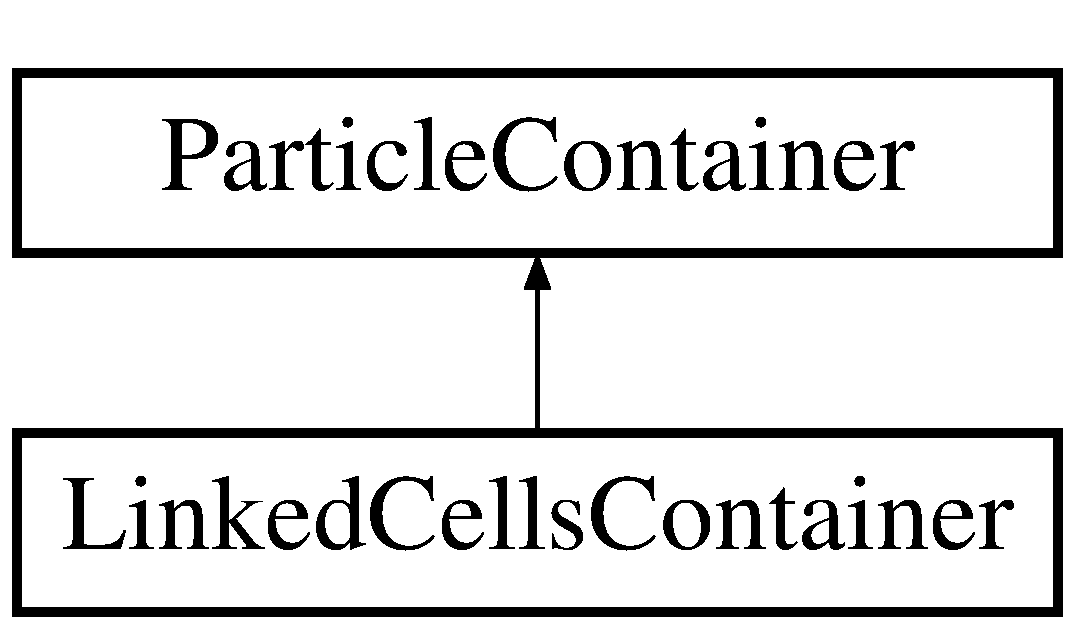
\includegraphics[height=2.000000cm]{classParticleContainer}
\end{center}
\end{figure}
\subsection*{Public Types}
\begin{DoxyCompactItemize}
\item 
enum \hyperlink{classParticleContainer_a2457078eafdf0fdd9eeb977e63aed6e8}{Force\+Method} \{ \hyperlink{classParticleContainer_a2457078eafdf0fdd9eeb977e63aed6e8aafc56f60001e371709e979276a58ead8}{Gravity}, 
\hyperlink{classParticleContainer_a2457078eafdf0fdd9eeb977e63aed6e8ada3883b657ac8c6a175c7946f0514e8e}{Lennard\+Jones}
 \}
\end{DoxyCompactItemize}
\subsection*{Public Member Functions}
\begin{DoxyCompactItemize}
\item 
\hyperlink{classParticleContainer_a64a701a902e5a4e97ae04acb9d63e20a}{Particle\+Container} (\hyperlink{classParticleContainer_a2457078eafdf0fdd9eeb977e63aed6e8}{Force\+Method} \hyperlink{classParticleContainer_a839c3ff474bfece04fcbb0ca3fe9a0f8}{fm}, double timestep=0.\+014, double \hyperlink{classParticleContainer_a64e8a768554b5b6126755e8a8e85f2f5}{Brownian\+Factor}=0.\+1)
\item 
virtual \hyperlink{classParticleContainer_a9629a8d31a3aa8c2fe944307c1263b66}{$\sim$\+Particle\+Container} ()
\item 
void \hyperlink{classParticleContainer_aac74c7e039e9c6342bcbab8b20dd1b06}{set\+DeltaT} (double timestep)
\item 
virtual void \hyperlink{classParticleContainer_af7fe938fddd10136945f99625e141149}{set\+Gravity} (\hyperlink{classutils_1_1Vector}{utils\+::\+Vector}$<$ double, 3 $>$ g)
\item 
virtual void \hyperlink{classParticleContainer_abdd289393fe11f1192a9eb79b01b2680}{set\+Membrane} (double stiff, double r\+\_\+zero, bool status, double tend)
\item 
virtual void \hyperlink{classParticleContainer_ae3f61f4d99b06782cfd978779ccc13bf}{set\+List} (std\+::list$<$ \hyperlink{classParticle}{Particle} $>$ plist)
\item 
virtual \hyperlink{classParticle}{Particle} $\ast$ \hyperlink{classParticleContainer_a13b860c91defffff1404e8e3c12766a8}{add\+Particle} (\hyperlink{classParticle}{Particle} \&p)
\item 
virtual void \hyperlink{classParticleContainer_a27c73f4106a4e38382dbf461e03bb5f1}{delete\+Particle} (\hyperlink{classParticle}{Particle} \&p)
\item 
virtual void \hyperlink{classParticleContainer_ae132e846bb2763712d4acca3095bcbfc}{test\+Force\+End} (double time)
\item 
virtual std\+::list$<$ \hyperlink{classParticle}{Particle} $>$ \& \hyperlink{classParticleContainer_a5b96e023a5b3c2507766cefa8f006c65}{get\+All} ()
\item 
virtual std\+::list$<$ \hyperlink{classParticle}{Particle} $\ast$ $>$ \hyperlink{classParticleContainer_a52ebfc06d0daa96fbeef945b43e4fe00}{get\+All\+Pointer} ()
\item 
virtual void \hyperlink{classParticleContainer_af5626526d41510605c20161df34de71b}{f\+Reset} ()
\item 
virtual void \hyperlink{classParticleContainer_a329f1c21166cb9722553a1845f9be4d0}{calculateF} ()
\item 
virtual void \hyperlink{classParticleContainer_abfe567934c1e3319a03377ebf7da2369}{calculateX} ()
\item 
virtual void \hyperlink{classParticleContainer_a7b436c3226f9eb05e86d895a7eab8b41}{calculateV} ()
\item 
\hyperlink{classutils_1_1Vector}{utils\+::\+Vector}$<$ double, 3 $>$ \hyperlink{classParticleContainer_a902a63a3c7758262aaec851a61557424}{calcF} (\hyperlink{classParticle}{Particle} \&p1, \hyperlink{classParticle}{Particle} \&p2)
\item 
void \hyperlink{classParticleContainer_a76b73383fadd0c6605bc44910357b5cd}{Harmonic\+Potential} (double k, double r\+\_\+zero)
\item 
\hyperlink{classutils_1_1Vector}{utils\+::\+Vector}$<$ double, 3 $>$ \hyperlink{classParticleContainer_a672e44d2fe6c69fd9f1e15b5aa3897f1}{calc\+Gravity} (\hyperlink{classParticle}{Particle} \&p1, \hyperlink{classParticle}{Particle} \&p2)
\item 
\hyperlink{classutils_1_1Vector}{utils\+::\+Vector}$<$ double, 3 $>$ \hyperlink{classParticleContainer_a8c64e42668cc829b2bc7bd7f12692c8c}{calc\+Lennard\+Jones} (\hyperlink{classParticle}{Particle} \&p1, \hyperlink{classParticle}{Particle} \&p2)
\item 
void \hyperlink{classParticleContainer_a5bd493f8fcdb9d4cf1f21c9a1108548f}{generate\+Cuboid} (int \hyperlink{classtype}{type}, \hyperlink{classutils_1_1Vector}{utils\+::\+Vector}$<$ double, 3 $>$ pos, \hyperlink{classutils_1_1Vector}{utils\+::\+Vector}$<$ int, 3 $>$ dim, double h, \hyperlink{classutils_1_1Vector}{utils\+::\+Vector}$<$ double, 3 $>$ v)
\item 
void \hyperlink{classParticleContainer_a1cddd777f83656d0593775612cf56af8}{generate\+Membrane} (int \hyperlink{classtype}{type}, double \hyperlink{classParticleContainer_a3a00b0487e24b68b5cedc29087221f00}{stiffness}, double r\+\_\+zero, double t\+\_\+end, \hyperlink{classutils_1_1Vector}{utils\+::\+Vector}$<$ double, 3 $>$ force, std\+::list$<$ \hyperlink{classutils_1_1Vector}{utils\+::\+Vector}$<$ int, 3 $>$$>$ coord\+\_\+force, \hyperlink{classutils_1_1Vector}{utils\+::\+Vector}$<$ double, 3 $>$ pos, \hyperlink{classutils_1_1Vector}{utils\+::\+Vector}$<$ int, 3 $>$ dim, double h, \hyperlink{classutils_1_1Vector}{utils\+::\+Vector}$<$ double, 3 $>$ v)
\item 
void \hyperlink{classParticleContainer_aa51fcd453b6fac96026ce942fe674454}{generate\+Sphere} (int \hyperlink{classtype}{type}, \hyperlink{classutils_1_1Vector}{utils\+::\+Vector}$<$ double, 3 $>$ pos, int r, double h, \hyperlink{classutils_1_1Vector}{utils\+::\+Vector}$<$ double, 3 $>$ v)
\item 
void \hyperlink{classParticleContainer_a7861f4a36ac905683eb741e4afe2e4b1}{set\+Temperature} (float T, bool ignoreY)
\end{DoxyCompactItemize}
\subsection*{Protected Attributes}
\begin{DoxyCompactItemize}
\item 
std\+::list$<$ \hyperlink{classParticle}{Particle} $>$ \hyperlink{classParticleContainer_aad341e230fc4533690e0db8a4c9126f4}{partlist}
\item 
double \hyperlink{classParticleContainer_a00ee8dcd9a5c11b54e8fc731d38b45fa}{delta\+\_\+t}
\item 
\hyperlink{classParticleContainer_a2457078eafdf0fdd9eeb977e63aed6e8}{Force\+Method} \hyperlink{classParticleContainer_a839c3ff474bfece04fcbb0ca3fe9a0f8}{fm}
\item 
\hyperlink{classutils_1_1Vector}{utils\+::\+Vector}$<$ double, 3 $>$(Particle\+Container\+::$\ast$ \hyperlink{classParticleContainer_a3827ee46dac1ac38cc1312c6e7dae493}{calc\+F\+Function} )(\hyperlink{classParticle}{Particle} \&, \hyperlink{classParticle}{Particle} \&)
\item 
double \hyperlink{classParticleContainer_a64e8a768554b5b6126755e8a8e85f2f5}{Brownian\+Factor}
\item 
double \hyperlink{classParticleContainer_a3a00b0487e24b68b5cedc29087221f00}{stiffness} = 0
\item 
double \hyperlink{classParticleContainer_a50a0c62bf198ef1e37fe5c4d64a4a95a}{r0} = 0
\item 
bool \hyperlink{classParticleContainer_a9a051bfdd0e558ad4637335406c14fad}{membrane\+\_\+active} = false
\item 
double \hyperlink{classParticleContainer_aaa12218c40cf5d8f2421d5cc09fcafc0}{t\+\_\+end\+\_\+force} = 0
\end{DoxyCompactItemize}


\subsection{Detailed Description}
Class to hold a set of particles. 



\subsection{Member Enumeration Documentation}
\index{Particle\+Container@{Particle\+Container}!Force\+Method@{Force\+Method}}
\index{Force\+Method@{Force\+Method}!Particle\+Container@{Particle\+Container}}
\subsubsection[{\texorpdfstring{Force\+Method}{ForceMethod}}]{\setlength{\rightskip}{0pt plus 5cm}enum {\bf Particle\+Container\+::\+Force\+Method}}\hypertarget{classParticleContainer_a2457078eafdf0fdd9eeb977e63aed6e8}{}\label{classParticleContainer_a2457078eafdf0fdd9eeb977e63aed6e8}
\begin{Desc}
\item[Enumerator]\par
\begin{description}
\index{Gravity@{Gravity}!Particle\+Container@{Particle\+Container}}\index{Particle\+Container@{Particle\+Container}!Gravity@{Gravity}}\item[{\em 
Gravity\hypertarget{classParticleContainer_a2457078eafdf0fdd9eeb977e63aed6e8aafc56f60001e371709e979276a58ead8}{}\label{classParticleContainer_a2457078eafdf0fdd9eeb977e63aed6e8aafc56f60001e371709e979276a58ead8}
}]\index{Lennard\+Jones@{Lennard\+Jones}!Particle\+Container@{Particle\+Container}}\index{Particle\+Container@{Particle\+Container}!Lennard\+Jones@{Lennard\+Jones}}\item[{\em 
Lennard\+Jones\hypertarget{classParticleContainer_a2457078eafdf0fdd9eeb977e63aed6e8ada3883b657ac8c6a175c7946f0514e8e}{}\label{classParticleContainer_a2457078eafdf0fdd9eeb977e63aed6e8ada3883b657ac8c6a175c7946f0514e8e}
}]\end{description}
\end{Desc}


\subsection{Constructor \& Destructor Documentation}
\index{Particle\+Container@{Particle\+Container}!Particle\+Container@{Particle\+Container}}
\index{Particle\+Container@{Particle\+Container}!Particle\+Container@{Particle\+Container}}
\subsubsection[{\texorpdfstring{Particle\+Container(\+Force\+Method fm, double timestep=0.\+014, double Brownian\+Factor=0.\+1)}{ParticleContainer(ForceMethod fm, double timestep=0.014, double BrownianFactor=0.1)}}]{\setlength{\rightskip}{0pt plus 5cm}Particle\+Container\+::\+Particle\+Container (
\begin{DoxyParamCaption}
\item[{enum {\bf Particle\+Container\+::\+Force\+Method}}]{fm, }
\item[{double}]{timestep = {\ttfamily 0.014}, }
\item[{double}]{Brownian\+Factor = {\ttfamily 0.1}}
\end{DoxyParamCaption}
)}\hypertarget{classParticleContainer_a64a701a902e5a4e97ae04acb9d63e20a}{}\label{classParticleContainer_a64a701a902e5a4e97ae04acb9d63e20a}
Constructor 
\begin{DoxyParams}{Parameters}
{\em f} & Function function to calculate the force between two particles \\
\hline
{\em timestep} & step between each step \\
\hline
{\em Brownian\+Factor} & the brownian Factor \\
\hline
\end{DoxyParams}
\index{Particle\+Container@{Particle\+Container}!````~Particle\+Container@{$\sim$\+Particle\+Container}}
\index{````~Particle\+Container@{$\sim$\+Particle\+Container}!Particle\+Container@{Particle\+Container}}
\subsubsection[{\texorpdfstring{$\sim$\+Particle\+Container()}{~ParticleContainer()}}]{\setlength{\rightskip}{0pt plus 5cm}Particle\+Container\+::$\sim$\+Particle\+Container (
\begin{DoxyParamCaption}
{}
\end{DoxyParamCaption}
)\hspace{0.3cm}{\ttfamily [virtual]}}\hypertarget{classParticleContainer_a9629a8d31a3aa8c2fe944307c1263b66}{}\label{classParticleContainer_a9629a8d31a3aa8c2fe944307c1263b66}


\subsection{Member Function Documentation}
\index{Particle\+Container@{Particle\+Container}!add\+Particle@{add\+Particle}}
\index{add\+Particle@{add\+Particle}!Particle\+Container@{Particle\+Container}}
\subsubsection[{\texorpdfstring{add\+Particle(\+Particle \&p)}{addParticle(Particle &p)}}]{\setlength{\rightskip}{0pt plus 5cm}{\bf Particle} $\ast$ Particle\+Container\+::add\+Particle (
\begin{DoxyParamCaption}
\item[{{\bf Particle} \&}]{p}
\end{DoxyParamCaption}
)\hspace{0.3cm}{\ttfamily [virtual]}}\hypertarget{classParticleContainer_a13b860c91defffff1404e8e3c12766a8}{}\label{classParticleContainer_a13b860c91defffff1404e8e3c12766a8}
add one particle to the container 
\begin{DoxyParams}{Parameters}
{\em p} & the particle to add \\
\hline
\end{DoxyParams}
\begin{DoxyReturn}{Returns}
a pointer to the newly created particle 
\end{DoxyReturn}


Reimplemented in \hyperlink{classLinkedCellsContainer_ac1987c930d49b2300a0f3509e282f2f1}{Linked\+Cells\+Container}.

\index{Particle\+Container@{Particle\+Container}!calcF@{calcF}}
\index{calcF@{calcF}!Particle\+Container@{Particle\+Container}}
\subsubsection[{\texorpdfstring{calc\+F(\+Particle \&p1, Particle \&p2)}{calcF(Particle &p1, Particle &p2)}}]{\setlength{\rightskip}{0pt plus 5cm}{\bf utils\+::\+Vector}$<$ double, 3 $>$ Particle\+Container\+::calcF (
\begin{DoxyParamCaption}
\item[{{\bf Particle} \&}]{p1, }
\item[{{\bf Particle} \&}]{p2}
\end{DoxyParamCaption}
)\hspace{0.3cm}{\ttfamily [inline]}}\hypertarget{classParticleContainer_a902a63a3c7758262aaec851a61557424}{}\label{classParticleContainer_a902a63a3c7758262aaec851a61557424}
calculate forces using selected function 
\begin{DoxyParams}{Parameters}
{\em p1} & first particle \\
\hline
{\em p2} & second particle \\
\hline
\end{DoxyParams}
\begin{DoxyReturn}{Returns}
vector containing forces 
\end{DoxyReturn}
\index{Particle\+Container@{Particle\+Container}!calc\+Gravity@{calc\+Gravity}}
\index{calc\+Gravity@{calc\+Gravity}!Particle\+Container@{Particle\+Container}}
\subsubsection[{\texorpdfstring{calc\+Gravity(\+Particle \&p1, Particle \&p2)}{calcGravity(Particle &p1, Particle &p2)}}]{\setlength{\rightskip}{0pt plus 5cm}{\bf utils\+::\+Vector}$<$ double, 3 $>$ Particle\+Container\+::calc\+Gravity (
\begin{DoxyParamCaption}
\item[{{\bf Particle} \&}]{p1, }
\item[{{\bf Particle} \&}]{p2}
\end{DoxyParamCaption}
)}\hypertarget{classParticleContainer_a672e44d2fe6c69fd9f1e15b5aa3897f1}{}\label{classParticleContainer_a672e44d2fe6c69fd9f1e15b5aa3897f1}
calculate forces using gravity 
\begin{DoxyParams}{Parameters}
{\em p1} & first particle \\
\hline
{\em p2} & second particle \\
\hline
\end{DoxyParams}
\begin{DoxyReturn}{Returns}
vector containing forces 
\end{DoxyReturn}
\index{Particle\+Container@{Particle\+Container}!calc\+Lennard\+Jones@{calc\+Lennard\+Jones}}
\index{calc\+Lennard\+Jones@{calc\+Lennard\+Jones}!Particle\+Container@{Particle\+Container}}
\subsubsection[{\texorpdfstring{calc\+Lennard\+Jones(\+Particle \&p1, Particle \&p2)}{calcLennardJones(Particle &p1, Particle &p2)}}]{\setlength{\rightskip}{0pt plus 5cm}{\bf utils\+::\+Vector}$<$ double, 3 $>$ Particle\+Container\+::calc\+Lennard\+Jones (
\begin{DoxyParamCaption}
\item[{{\bf Particle} \&}]{p1, }
\item[{{\bf Particle} \&}]{p2}
\end{DoxyParamCaption}
)}\hypertarget{classParticleContainer_a8c64e42668cc829b2bc7bd7f12692c8c}{}\label{classParticleContainer_a8c64e42668cc829b2bc7bd7f12692c8c}
calculate forces using Lennard-\/\+Jones Potential 
\begin{DoxyParams}{Parameters}
{\em p1} & first particle \\
\hline
{\em p2} & second particle \\
\hline
\end{DoxyParams}
\begin{DoxyReturn}{Returns}
vector containing forces 
\end{DoxyReturn}
\index{Particle\+Container@{Particle\+Container}!calculateF@{calculateF}}
\index{calculateF@{calculateF}!Particle\+Container@{Particle\+Container}}
\subsubsection[{\texorpdfstring{calculate\+F()}{calculateF()}}]{\setlength{\rightskip}{0pt plus 5cm}void Particle\+Container\+::calculateF (
\begin{DoxyParamCaption}
{}
\end{DoxyParamCaption}
)\hspace{0.3cm}{\ttfamily [virtual]}}\hypertarget{classParticleContainer_a329f1c21166cb9722553a1845f9be4d0}{}\label{classParticleContainer_a329f1c21166cb9722553a1845f9be4d0}
calculate the force for all particles 

Reimplemented in \hyperlink{classLinkedCellsContainer_aaccb110aaed18cb2986a51e970e86fa4}{Linked\+Cells\+Container}.

\index{Particle\+Container@{Particle\+Container}!calculateV@{calculateV}}
\index{calculateV@{calculateV}!Particle\+Container@{Particle\+Container}}
\subsubsection[{\texorpdfstring{calculate\+V()}{calculateV()}}]{\setlength{\rightskip}{0pt plus 5cm}void Particle\+Container\+::calculateV (
\begin{DoxyParamCaption}
{}
\end{DoxyParamCaption}
)\hspace{0.3cm}{\ttfamily [virtual]}}\hypertarget{classParticleContainer_a7b436c3226f9eb05e86d895a7eab8b41}{}\label{classParticleContainer_a7b436c3226f9eb05e86d895a7eab8b41}
calculate the position for all particles using the Velocity-\/\+Stoermer-\/\+Verlet-\/\+Algorithm 

Reimplemented in \hyperlink{classLinkedCellsContainer_a5b9a6d9b726bda76160aaf7fbaffa821}{Linked\+Cells\+Container}.

\index{Particle\+Container@{Particle\+Container}!calculateX@{calculateX}}
\index{calculateX@{calculateX}!Particle\+Container@{Particle\+Container}}
\subsubsection[{\texorpdfstring{calculate\+X()}{calculateX()}}]{\setlength{\rightskip}{0pt plus 5cm}void Particle\+Container\+::calculateX (
\begin{DoxyParamCaption}
{}
\end{DoxyParamCaption}
)\hspace{0.3cm}{\ttfamily [virtual]}}\hypertarget{classParticleContainer_abfe567934c1e3319a03377ebf7da2369}{}\label{classParticleContainer_abfe567934c1e3319a03377ebf7da2369}
calculate the position for all particles using the Velocity-\/\+Stoermer-\/\+Verlet-\/\+Algorithm 

Reimplemented in \hyperlink{classLinkedCellsContainer_ad2862569c3377347adfc06964ab7d966}{Linked\+Cells\+Container}.

\index{Particle\+Container@{Particle\+Container}!delete\+Particle@{delete\+Particle}}
\index{delete\+Particle@{delete\+Particle}!Particle\+Container@{Particle\+Container}}
\subsubsection[{\texorpdfstring{delete\+Particle(\+Particle \&p)}{deleteParticle(Particle &p)}}]{\setlength{\rightskip}{0pt plus 5cm}void Particle\+Container\+::delete\+Particle (
\begin{DoxyParamCaption}
\item[{{\bf Particle} \&}]{p}
\end{DoxyParamCaption}
)\hspace{0.3cm}{\ttfamily [virtual]}}\hypertarget{classParticleContainer_a27c73f4106a4e38382dbf461e03bb5f1}{}\label{classParticleContainer_a27c73f4106a4e38382dbf461e03bb5f1}
remove a particle from the container 
\begin{DoxyParams}{Parameters}
{\em p} & the particle to remove \\
\hline
\end{DoxyParams}


Reimplemented in \hyperlink{classLinkedCellsContainer_a6466835bf54973f4c7ec916c9b1f089b}{Linked\+Cells\+Container}.

\index{Particle\+Container@{Particle\+Container}!f\+Reset@{f\+Reset}}
\index{f\+Reset@{f\+Reset}!Particle\+Container@{Particle\+Container}}
\subsubsection[{\texorpdfstring{f\+Reset()}{fReset()}}]{\setlength{\rightskip}{0pt plus 5cm}void Particle\+Container\+::f\+Reset (
\begin{DoxyParamCaption}
{}
\end{DoxyParamCaption}
)\hspace{0.3cm}{\ttfamily [virtual]}}\hypertarget{classParticleContainer_af5626526d41510605c20161df34de71b}{}\label{classParticleContainer_af5626526d41510605c20161df34de71b}
set the force to all particles according to gravity force 

Reimplemented in \hyperlink{classLinkedCellsContainer_ae2ebc865c7e07122e2ab5985182d82bc}{Linked\+Cells\+Container}.

\index{Particle\+Container@{Particle\+Container}!generate\+Cuboid@{generate\+Cuboid}}
\index{generate\+Cuboid@{generate\+Cuboid}!Particle\+Container@{Particle\+Container}}
\subsubsection[{\texorpdfstring{generate\+Cuboid(int type, utils\+::\+Vector$<$ double, 3 $>$ pos, utils\+::\+Vector$<$ int, 3 $>$ dim, double h, utils\+::\+Vector$<$ double, 3 $>$ v)}{generateCuboid(int type, utils::Vector< double, 3 > pos, utils::Vector< int, 3 > dim, double h, utils::Vector< double, 3 > v)}}]{\setlength{\rightskip}{0pt plus 5cm}void Particle\+Container\+::generate\+Cuboid (
\begin{DoxyParamCaption}
\item[{int}]{type, }
\item[{{\bf utils\+::\+Vector}$<$ double, 3 $>$}]{pos, }
\item[{{\bf utils\+::\+Vector}$<$ int, 3 $>$}]{dim, }
\item[{double}]{h, }
\item[{{\bf utils\+::\+Vector}$<$ double, 3 $>$}]{v}
\end{DoxyParamCaption}
)}\hypertarget{classParticleContainer_a5bd493f8fcdb9d4cf1f21c9a1108548f}{}\label{classParticleContainer_a5bd493f8fcdb9d4cf1f21c9a1108548f}
generates a cuboid of particles 
\begin{DoxyParams}{Parameters}
{\em type} & type of each particle \\
\hline
{\em pos} & coordinates of lower left front-\/side corner \\
\hline
{\em dim} & number of particles in each dimension \\
\hline
{\em h} & mesh width \\
\hline
{\em v} & velocity of each particle \\
\hline
\end{DoxyParams}
\index{Particle\+Container@{Particle\+Container}!generate\+Membrane@{generate\+Membrane}}
\index{generate\+Membrane@{generate\+Membrane}!Particle\+Container@{Particle\+Container}}
\subsubsection[{\texorpdfstring{generate\+Membrane(int type, double stiffness, double r\+\_\+zero, double t\+\_\+end, utils\+::\+Vector$<$ double, 3 $>$ force, std\+::list$<$ utils\+::\+Vector$<$ int, 3 $>$$>$ coord\+\_\+force, utils\+::\+Vector$<$ double, 3 $>$ pos, utils\+::\+Vector$<$ int, 3 $>$ dim, double h, utils\+::\+Vector$<$ double, 3 $>$ v)}{generateMembrane(int type, double stiffness, double r_zero, double t_end, utils::Vector< double, 3 > force, std::list< utils::Vector< int, 3 >> coord_force, utils::Vector< double, 3 > pos, utils::Vector< int, 3 > dim, double h, utils::Vector< double, 3 > v)}}]{\setlength{\rightskip}{0pt plus 5cm}void Particle\+Container\+::generate\+Membrane (
\begin{DoxyParamCaption}
\item[{int}]{type, }
\item[{double}]{stiffness, }
\item[{double}]{r\+\_\+zero, }
\item[{double}]{t\+\_\+end, }
\item[{{\bf utils\+::\+Vector}$<$ double, 3 $>$}]{force, }
\item[{std\+::list$<$ {\bf utils\+::\+Vector}$<$ int, 3 $>$$>$}]{coord\+\_\+force, }
\item[{{\bf utils\+::\+Vector}$<$ double, 3 $>$}]{pos, }
\item[{{\bf utils\+::\+Vector}$<$ int, 3 $>$}]{dim, }
\item[{double}]{h, }
\item[{{\bf utils\+::\+Vector}$<$ double, 3 $>$}]{v}
\end{DoxyParamCaption}
)}\hypertarget{classParticleContainer_a1cddd777f83656d0593775612cf56af8}{}\label{classParticleContainer_a1cddd777f83656d0593775612cf56af8}
generates a cuboid of membrane particles 
\begin{DoxyParams}{Parameters}
{\em stiffness} & stiffness k of the membrane \\
\hline
{\em r\+\_\+zero} & average bond length of a molecule pair \\
\hline
{\em t\+\_\+end} & time when the force up should disappear \\
\hline
{\em force} & force acting on certain particles in the membrane \\
\hline
{\em force\+\_\+coord} & list of mesh coordinates of the particles supporting an external force \\
\hline
{\em type} & type of each particle \\
\hline
{\em pos} & coordinates of lower left front-\/side corner \\
\hline
{\em dim} & number of particles in each dimension \\
\hline
{\em h} & mesh width \\
\hline
{\em v} & velocity of each particle \\
\hline
\end{DoxyParams}
\index{Particle\+Container@{Particle\+Container}!generate\+Sphere@{generate\+Sphere}}
\index{generate\+Sphere@{generate\+Sphere}!Particle\+Container@{Particle\+Container}}
\subsubsection[{\texorpdfstring{generate\+Sphere(int type, utils\+::\+Vector$<$ double, 3 $>$ pos, int r, double h, utils\+::\+Vector$<$ double, 3 $>$ v)}{generateSphere(int type, utils::Vector< double, 3 > pos, int r, double h, utils::Vector< double, 3 > v)}}]{\setlength{\rightskip}{0pt plus 5cm}void Particle\+Container\+::generate\+Sphere (
\begin{DoxyParamCaption}
\item[{int}]{type, }
\item[{{\bf utils\+::\+Vector}$<$ double, 3 $>$}]{pos, }
\item[{int}]{r, }
\item[{double}]{h, }
\item[{{\bf utils\+::\+Vector}$<$ double, 3 $>$}]{v}
\end{DoxyParamCaption}
)}\hypertarget{classParticleContainer_aa51fcd453b6fac96026ce942fe674454}{}\label{classParticleContainer_aa51fcd453b6fac96026ce942fe674454}
generates a sphere of particles 
\begin{DoxyParams}{Parameters}
{\em type} & type of each particle \\
\hline
{\em pos} & coordinates of the center of sphere \\
\hline
{\em r} & number of particles as radius \\
\hline
{\em h} & mesh width \\
\hline
{\em m} & mass of each particle \\
\hline
{\em v} & velocity of each particle \\
\hline
\end{DoxyParams}
\index{Particle\+Container@{Particle\+Container}!get\+All@{get\+All}}
\index{get\+All@{get\+All}!Particle\+Container@{Particle\+Container}}
\subsubsection[{\texorpdfstring{get\+All()}{getAll()}}]{\setlength{\rightskip}{0pt plus 5cm}std\+::list$<$ {\bf Particle} $>$ \& Particle\+Container\+::get\+All (
\begin{DoxyParamCaption}
{}
\end{DoxyParamCaption}
)\hspace{0.3cm}{\ttfamily [virtual]}}\hypertarget{classParticleContainer_a5b96e023a5b3c2507766cefa8f006c65}{}\label{classParticleContainer_a5b96e023a5b3c2507766cefa8f006c65}
get a list of all particle in the container \begin{DoxyReturn}{Returns}
list of all particles 
\end{DoxyReturn}


Reimplemented in \hyperlink{classLinkedCellsContainer_a33feabbd2ffc9f8cb34ec237e057b7bc}{Linked\+Cells\+Container}.

\index{Particle\+Container@{Particle\+Container}!get\+All\+Pointer@{get\+All\+Pointer}}
\index{get\+All\+Pointer@{get\+All\+Pointer}!Particle\+Container@{Particle\+Container}}
\subsubsection[{\texorpdfstring{get\+All\+Pointer()}{getAllPointer()}}]{\setlength{\rightskip}{0pt plus 5cm}std\+::list$<$ {\bf Particle} $\ast$ $>$ Particle\+Container\+::get\+All\+Pointer (
\begin{DoxyParamCaption}
{}
\end{DoxyParamCaption}
)\hspace{0.3cm}{\ttfamily [virtual]}}\hypertarget{classParticleContainer_a52ebfc06d0daa96fbeef945b43e4fe00}{}\label{classParticleContainer_a52ebfc06d0daa96fbeef945b43e4fe00}
get a list of pointer to all particle in the container \begin{DoxyReturn}{Returns}
list of all particles 
\end{DoxyReturn}


Reimplemented in \hyperlink{classLinkedCellsContainer_a0b3b6c216a529189b58b05991079bb21}{Linked\+Cells\+Container}.

\index{Particle\+Container@{Particle\+Container}!Harmonic\+Potential@{Harmonic\+Potential}}
\index{Harmonic\+Potential@{Harmonic\+Potential}!Particle\+Container@{Particle\+Container}}
\subsubsection[{\texorpdfstring{Harmonic\+Potential(double k, double r\+\_\+zero)}{HarmonicPotential(double k, double r_zero)}}]{\setlength{\rightskip}{0pt plus 5cm}void Particle\+Container\+::\+Harmonic\+Potential (
\begin{DoxyParamCaption}
\item[{double}]{k, }
\item[{double}]{r\+\_\+zero}
\end{DoxyParamCaption}
)}\hypertarget{classParticleContainer_a76b73383fadd0c6605bc44910357b5cd}{}\label{classParticleContainer_a76b73383fadd0c6605bc44910357b5cd}
Calculate forces acting in a membrane 
\begin{DoxyParams}{Parameters}
{\em p} & particle \\
\hline
{\em k} & Stiffness of the membrane \\
\hline
{\em r0} & average bond length \\
\hline
\end{DoxyParams}
\index{Particle\+Container@{Particle\+Container}!set\+DeltaT@{set\+DeltaT}}
\index{set\+DeltaT@{set\+DeltaT}!Particle\+Container@{Particle\+Container}}
\subsubsection[{\texorpdfstring{set\+Delta\+T(double timestep)}{setDeltaT(double timestep)}}]{\setlength{\rightskip}{0pt plus 5cm}void Particle\+Container\+::set\+DeltaT (
\begin{DoxyParamCaption}
\item[{double}]{timestep}
\end{DoxyParamCaption}
)}\hypertarget{classParticleContainer_aac74c7e039e9c6342bcbab8b20dd1b06}{}\label{classParticleContainer_aac74c7e039e9c6342bcbab8b20dd1b06}
set the timestep 
\begin{DoxyParams}{Parameters}
{\em timestep} & time between steps \\
\hline
\end{DoxyParams}
\index{Particle\+Container@{Particle\+Container}!set\+Gravity@{set\+Gravity}}
\index{set\+Gravity@{set\+Gravity}!Particle\+Container@{Particle\+Container}}
\subsubsection[{\texorpdfstring{set\+Gravity(utils\+::\+Vector$<$ double, 3 $>$ g)}{setGravity(utils::Vector< double, 3 > g)}}]{\setlength{\rightskip}{0pt plus 5cm}void Particle\+Container\+::set\+Gravity (
\begin{DoxyParamCaption}
\item[{{\bf utils\+::\+Vector}$<$ double, 3 $>$}]{g}
\end{DoxyParamCaption}
)\hspace{0.3cm}{\ttfamily [virtual]}}\hypertarget{classParticleContainer_af7fe938fddd10136945f99625e141149}{}\label{classParticleContainer_af7fe938fddd10136945f99625e141149}
set the gravitational force 
\begin{DoxyParams}{Parameters}
{\em g} & the gravitational acceleration \\
\hline
\end{DoxyParams}


Reimplemented in \hyperlink{classLinkedCellsContainer_a25d0ac927ce692ae3bf944a67f86682a}{Linked\+Cells\+Container}.

\index{Particle\+Container@{Particle\+Container}!set\+List@{set\+List}}
\index{set\+List@{set\+List}!Particle\+Container@{Particle\+Container}}
\subsubsection[{\texorpdfstring{set\+List(std\+::list$<$ Particle $>$ plist)}{setList(std::list< Particle > plist)}}]{\setlength{\rightskip}{0pt plus 5cm}void Particle\+Container\+::set\+List (
\begin{DoxyParamCaption}
\item[{std\+::list$<$ {\bf Particle} $>$}]{plist}
\end{DoxyParamCaption}
)\hspace{0.3cm}{\ttfamily [virtual]}}\hypertarget{classParticleContainer_ae3f61f4d99b06782cfd978779ccc13bf}{}\label{classParticleContainer_ae3f61f4d99b06782cfd978779ccc13bf}
define all particles in the container 
\begin{DoxyParams}{Parameters}
{\em plist} & the list to fill container \\
\hline
\end{DoxyParams}


Reimplemented in \hyperlink{classLinkedCellsContainer_a0c54230125a031821a99fc39b15e6d60}{Linked\+Cells\+Container}.

\index{Particle\+Container@{Particle\+Container}!set\+Membrane@{set\+Membrane}}
\index{set\+Membrane@{set\+Membrane}!Particle\+Container@{Particle\+Container}}
\subsubsection[{\texorpdfstring{set\+Membrane(double stiff, double r\+\_\+zero, bool status, double tend)}{setMembrane(double stiff, double r_zero, bool status, double tend)}}]{\setlength{\rightskip}{0pt plus 5cm}void Particle\+Container\+::set\+Membrane (
\begin{DoxyParamCaption}
\item[{double}]{stiff, }
\item[{double}]{r\+\_\+zero, }
\item[{bool}]{status, }
\item[{double}]{tend}
\end{DoxyParamCaption}
)\hspace{0.3cm}{\ttfamily [virtual]}}\hypertarget{classParticleContainer_abdd289393fe11f1192a9eb79b01b2680}{}\label{classParticleContainer_abdd289393fe11f1192a9eb79b01b2680}
sets the membrane parameters 
\begin{DoxyParams}{Parameters}
{\em stiff} & membrane stiffness \\
\hline
{\em r\+\_\+zero} & average bond lenght \\
\hline
{\em status} & whether the membrane is active or not \\
\hline
{\em tend} & force t\+\_\+end \\
\hline
\end{DoxyParams}


Reimplemented in \hyperlink{classLinkedCellsContainer_a831a33f6b4f90f71396474a99f985575}{Linked\+Cells\+Container}.

\index{Particle\+Container@{Particle\+Container}!set\+Temperature@{set\+Temperature}}
\index{set\+Temperature@{set\+Temperature}!Particle\+Container@{Particle\+Container}}
\subsubsection[{\texorpdfstring{set\+Temperature(float T, bool ignore\+Y)}{setTemperature(float T, bool ignoreY)}}]{\setlength{\rightskip}{0pt plus 5cm}void Particle\+Container\+::set\+Temperature (
\begin{DoxyParamCaption}
\item[{float}]{T, }
\item[{bool}]{ignoreY}
\end{DoxyParamCaption}
)}\hypertarget{classParticleContainer_a7861f4a36ac905683eb741e4afe2e4b1}{}\label{classParticleContainer_a7861f4a36ac905683eb741e4afe2e4b1}
add a thermostat which regulate the temperature to T 
\begin{DoxyParams}{Parameters}
{\em T} & new temperature \\
\hline
{\em ignoreY} & true if y-\/component is ignored \\
\hline
\end{DoxyParams}
\index{Particle\+Container@{Particle\+Container}!test\+Force\+End@{test\+Force\+End}}
\index{test\+Force\+End@{test\+Force\+End}!Particle\+Container@{Particle\+Container}}
\subsubsection[{\texorpdfstring{test\+Force\+End(double time)}{testForceEnd(double time)}}]{\setlength{\rightskip}{0pt plus 5cm}void Particle\+Container\+::test\+Force\+End (
\begin{DoxyParamCaption}
\item[{double}]{time}
\end{DoxyParamCaption}
)\hspace{0.3cm}{\ttfamily [virtual]}}\hypertarget{classParticleContainer_ae132e846bb2763712d4acca3095bcbfc}{}\label{classParticleContainer_ae132e846bb2763712d4acca3095bcbfc}
tests if the force up should be switched of 
\begin{DoxyParams}{Parameters}
{\em time} & current simulation time \\
\hline
\end{DoxyParams}


Reimplemented in \hyperlink{classLinkedCellsContainer_a0dc45c921ad11aa2424b49ada44a0dfe}{Linked\+Cells\+Container}.



\subsection{Member Data Documentation}
\index{Particle\+Container@{Particle\+Container}!Brownian\+Factor@{Brownian\+Factor}}
\index{Brownian\+Factor@{Brownian\+Factor}!Particle\+Container@{Particle\+Container}}
\subsubsection[{\texorpdfstring{Brownian\+Factor}{BrownianFactor}}]{\setlength{\rightskip}{0pt plus 5cm}double Particle\+Container\+::\+Brownian\+Factor\hspace{0.3cm}{\ttfamily [protected]}}\hypertarget{classParticleContainer_a64e8a768554b5b6126755e8a8e85f2f5}{}\label{classParticleContainer_a64e8a768554b5b6126755e8a8e85f2f5}
\index{Particle\+Container@{Particle\+Container}!calc\+F\+Function@{calc\+F\+Function}}
\index{calc\+F\+Function@{calc\+F\+Function}!Particle\+Container@{Particle\+Container}}
\subsubsection[{\texorpdfstring{calc\+F\+Function}{calcFFunction}}]{\setlength{\rightskip}{0pt plus 5cm}{\bf utils\+::\+Vector}$<$double,3$>$(Particle\+Container\+::$\ast$ Particle\+Container\+::calc\+F\+Function) ({\bf Particle} \&, {\bf Particle} \&)\hspace{0.3cm}{\ttfamily [protected]}}\hypertarget{classParticleContainer_a3827ee46dac1ac38cc1312c6e7dae493}{}\label{classParticleContainer_a3827ee46dac1ac38cc1312c6e7dae493}
\index{Particle\+Container@{Particle\+Container}!delta\+\_\+t@{delta\+\_\+t}}
\index{delta\+\_\+t@{delta\+\_\+t}!Particle\+Container@{Particle\+Container}}
\subsubsection[{\texorpdfstring{delta\+\_\+t}{delta_t}}]{\setlength{\rightskip}{0pt plus 5cm}double Particle\+Container\+::delta\+\_\+t\hspace{0.3cm}{\ttfamily [protected]}}\hypertarget{classParticleContainer_a00ee8dcd9a5c11b54e8fc731d38b45fa}{}\label{classParticleContainer_a00ee8dcd9a5c11b54e8fc731d38b45fa}
\index{Particle\+Container@{Particle\+Container}!fm@{fm}}
\index{fm@{fm}!Particle\+Container@{Particle\+Container}}
\subsubsection[{\texorpdfstring{fm}{fm}}]{\setlength{\rightskip}{0pt plus 5cm}{\bf Force\+Method} Particle\+Container\+::fm\hspace{0.3cm}{\ttfamily [protected]}}\hypertarget{classParticleContainer_a839c3ff474bfece04fcbb0ca3fe9a0f8}{}\label{classParticleContainer_a839c3ff474bfece04fcbb0ca3fe9a0f8}
\index{Particle\+Container@{Particle\+Container}!membrane\+\_\+active@{membrane\+\_\+active}}
\index{membrane\+\_\+active@{membrane\+\_\+active}!Particle\+Container@{Particle\+Container}}
\subsubsection[{\texorpdfstring{membrane\+\_\+active}{membrane_active}}]{\setlength{\rightskip}{0pt plus 5cm}bool Particle\+Container\+::membrane\+\_\+active = false\hspace{0.3cm}{\ttfamily [protected]}}\hypertarget{classParticleContainer_a9a051bfdd0e558ad4637335406c14fad}{}\label{classParticleContainer_a9a051bfdd0e558ad4637335406c14fad}
\index{Particle\+Container@{Particle\+Container}!partlist@{partlist}}
\index{partlist@{partlist}!Particle\+Container@{Particle\+Container}}
\subsubsection[{\texorpdfstring{partlist}{partlist}}]{\setlength{\rightskip}{0pt plus 5cm}std\+::list$<${\bf Particle}$>$ Particle\+Container\+::partlist\hspace{0.3cm}{\ttfamily [protected]}}\hypertarget{classParticleContainer_aad341e230fc4533690e0db8a4c9126f4}{}\label{classParticleContainer_aad341e230fc4533690e0db8a4c9126f4}
\index{Particle\+Container@{Particle\+Container}!r0@{r0}}
\index{r0@{r0}!Particle\+Container@{Particle\+Container}}
\subsubsection[{\texorpdfstring{r0}{r0}}]{\setlength{\rightskip}{0pt plus 5cm}double Particle\+Container\+::r0 = 0\hspace{0.3cm}{\ttfamily [protected]}}\hypertarget{classParticleContainer_a50a0c62bf198ef1e37fe5c4d64a4a95a}{}\label{classParticleContainer_a50a0c62bf198ef1e37fe5c4d64a4a95a}
\index{Particle\+Container@{Particle\+Container}!stiffness@{stiffness}}
\index{stiffness@{stiffness}!Particle\+Container@{Particle\+Container}}
\subsubsection[{\texorpdfstring{stiffness}{stiffness}}]{\setlength{\rightskip}{0pt plus 5cm}double Particle\+Container\+::stiffness = 0\hspace{0.3cm}{\ttfamily [protected]}}\hypertarget{classParticleContainer_a3a00b0487e24b68b5cedc29087221f00}{}\label{classParticleContainer_a3a00b0487e24b68b5cedc29087221f00}
\index{Particle\+Container@{Particle\+Container}!t\+\_\+end\+\_\+force@{t\+\_\+end\+\_\+force}}
\index{t\+\_\+end\+\_\+force@{t\+\_\+end\+\_\+force}!Particle\+Container@{Particle\+Container}}
\subsubsection[{\texorpdfstring{t\+\_\+end\+\_\+force}{t_end_force}}]{\setlength{\rightskip}{0pt plus 5cm}double Particle\+Container\+::t\+\_\+end\+\_\+force = 0\hspace{0.3cm}{\ttfamily [protected]}}\hypertarget{classParticleContainer_aaa12218c40cf5d8f2421d5cc09fcafc0}{}\label{classParticleContainer_aaa12218c40cf5d8f2421d5cc09fcafc0}


The documentation for this class was generated from the following files\+:\begin{DoxyCompactItemize}
\item 
src/\hyperlink{ParticleContainer_8h}{Particle\+Container.\+h}\item 
src/\hyperlink{ParticleContainer_8cpp}{Particle\+Container.\+cpp}\end{DoxyCompactItemize}

\hypertarget{classParticleContainerTest}{}\section{Particle\+Container\+Test Class Reference}
\label{classParticleContainerTest}\index{Particle\+Container\+Test@{Particle\+Container\+Test}}


Test\+Suite for \hyperlink{classParticleContainer}{Particle\+Container}.  




{\ttfamily \#include $<$Particle\+Container\+Test.\+h$>$}

Inheritance diagram for Particle\+Container\+Test\+:\begin{figure}[H]
\begin{center}
\leavevmode
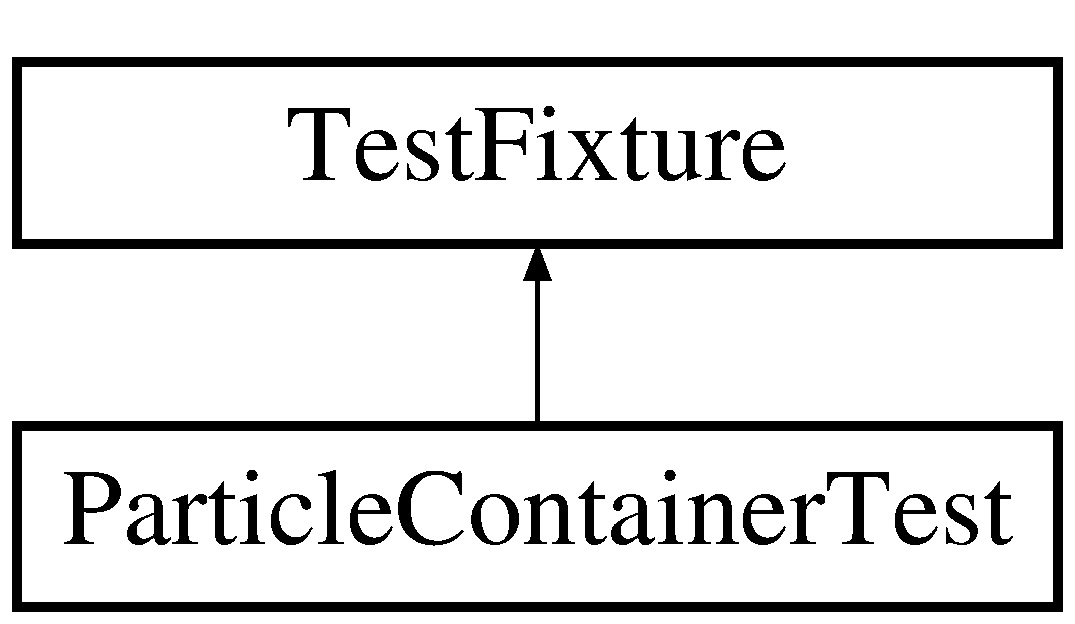
\includegraphics[height=2.000000cm]{classParticleContainerTest}
\end{center}
\end{figure}
\subsection*{Public Member Functions}
\begin{DoxyCompactItemize}
\item 
void \hyperlink{classParticleContainerTest_a114674bf106f1237eb8e5d0afa2cead0}{set\+Up} ()
\item 
void \hyperlink{classParticleContainerTest_a3a4921704ae21a160f9b6c5e086dca5c}{add\+Particle\+Test} ()
\item 
void \hyperlink{classParticleContainerTest_a310fd3941f72ccbed84840167828152d}{delete\+Particle\+Test} ()
\item 
void \hyperlink{classParticleContainerTest_aedf461c006cedb3a707d355d9c472107}{fclear\+Test} ()
\item 
void \hyperlink{classParticleContainerTest_a623a17cee1bfde4ab23127163509d5b4}{calculate\+F\+Test} ()
\item 
void \hyperlink{classParticleContainerTest_a18827c80c7e7faba9bb992c38b95d718}{Generate\+Cuboid\+Test} ()
\item 
\hyperlink{classParticleContainerTest_ac9c892489b33cc0fb091eca01677f74e}{Particle\+Container\+Test} ()
\item 
virtual \hyperlink{classParticleContainerTest_a6fff30944bc8d19c2a838ac0735222fc}{$\sim$\+Particle\+Container\+Test} ()
\end{DoxyCompactItemize}
\subsection*{Private Member Functions}
\begin{DoxyCompactItemize}
\item 
\hyperlink{classParticleContainerTest_ae9afd034703d0c21b00e498da7f263f3}{C\+P\+P\+U\+N\+I\+T\+\_\+\+T\+E\+S\+T\+\_\+\+S\+U\+I\+TE} (\hyperlink{classParticleContainerTest}{Particle\+Container\+Test})
\item 
\hyperlink{classParticleContainerTest_a48b201cc96992dd146d1ef89b84236a3}{C\+P\+P\+U\+N\+I\+T\+\_\+\+T\+E\+ST} (\hyperlink{classParticleContainerTest_a3a4921704ae21a160f9b6c5e086dca5c}{add\+Particle\+Test})
\item 
\hyperlink{classParticleContainerTest_a781a20cd143fb3691ecdc153e9f64a3a}{C\+P\+P\+U\+N\+I\+T\+\_\+\+T\+E\+ST} (\hyperlink{classParticleContainerTest_a310fd3941f72ccbed84840167828152d}{delete\+Particle\+Test})
\item 
\hyperlink{classParticleContainerTest_ac80b1adae5486191918fc38b5deeb156}{C\+P\+P\+U\+N\+I\+T\+\_\+\+T\+E\+ST} (\hyperlink{classParticleContainerTest_aedf461c006cedb3a707d355d9c472107}{fclear\+Test})
\item 
\hyperlink{classParticleContainerTest_abd24480618839a358f528f1db886e22b}{C\+P\+P\+U\+N\+I\+T\+\_\+\+T\+E\+ST} (\hyperlink{classParticleContainerTest_a623a17cee1bfde4ab23127163509d5b4}{calculate\+F\+Test})
\item 
\hyperlink{classParticleContainerTest_a4ccbd4c5f5e2947d3dcb14da5410dcdc}{C\+P\+P\+U\+N\+I\+T\+\_\+\+T\+E\+ST} (\hyperlink{classParticleContainerTest_a18827c80c7e7faba9bb992c38b95d718}{Generate\+Cuboid\+Test})
\item 
\hyperlink{classParticleContainerTest_aa276cd865efaccb4410ed6beb8d0ba4f}{C\+P\+P\+U\+N\+I\+T\+\_\+\+T\+E\+S\+T\+\_\+\+S\+U\+I\+T\+E\+\_\+\+E\+ND} ()
\end{DoxyCompactItemize}


\subsection{Detailed Description}
Test\+Suite for \hyperlink{classParticleContainer}{Particle\+Container}. 

\subsection{Constructor \& Destructor Documentation}
\index{Particle\+Container\+Test@{Particle\+Container\+Test}!Particle\+Container\+Test@{Particle\+Container\+Test}}
\index{Particle\+Container\+Test@{Particle\+Container\+Test}!Particle\+Container\+Test@{Particle\+Container\+Test}}
\subsubsection[{\texorpdfstring{Particle\+Container\+Test()}{ParticleContainerTest()}}]{\setlength{\rightskip}{0pt plus 5cm}Particle\+Container\+Test\+::\+Particle\+Container\+Test (
\begin{DoxyParamCaption}
{}
\end{DoxyParamCaption}
)}\hypertarget{classParticleContainerTest_ac9c892489b33cc0fb091eca01677f74e}{}\label{classParticleContainerTest_ac9c892489b33cc0fb091eca01677f74e}
\index{Particle\+Container\+Test@{Particle\+Container\+Test}!````~Particle\+Container\+Test@{$\sim$\+Particle\+Container\+Test}}
\index{````~Particle\+Container\+Test@{$\sim$\+Particle\+Container\+Test}!Particle\+Container\+Test@{Particle\+Container\+Test}}
\subsubsection[{\texorpdfstring{$\sim$\+Particle\+Container\+Test()}{~ParticleContainerTest()}}]{\setlength{\rightskip}{0pt plus 5cm}Particle\+Container\+Test\+::$\sim$\+Particle\+Container\+Test (
\begin{DoxyParamCaption}
{}
\end{DoxyParamCaption}
)\hspace{0.3cm}{\ttfamily [virtual]}}\hypertarget{classParticleContainerTest_a6fff30944bc8d19c2a838ac0735222fc}{}\label{classParticleContainerTest_a6fff30944bc8d19c2a838ac0735222fc}


\subsection{Member Function Documentation}
\index{Particle\+Container\+Test@{Particle\+Container\+Test}!add\+Particle\+Test@{add\+Particle\+Test}}
\index{add\+Particle\+Test@{add\+Particle\+Test}!Particle\+Container\+Test@{Particle\+Container\+Test}}
\subsubsection[{\texorpdfstring{add\+Particle\+Test()}{addParticleTest()}}]{\setlength{\rightskip}{0pt plus 5cm}void Particle\+Container\+Test\+::add\+Particle\+Test (
\begin{DoxyParamCaption}
{}
\end{DoxyParamCaption}
)}\hypertarget{classParticleContainerTest_a3a4921704ae21a160f9b6c5e086dca5c}{}\label{classParticleContainerTest_a3a4921704ae21a160f9b6c5e086dca5c}
Tests if particles are added, but copies are ignored \index{Particle\+Container\+Test@{Particle\+Container\+Test}!calculate\+F\+Test@{calculate\+F\+Test}}
\index{calculate\+F\+Test@{calculate\+F\+Test}!Particle\+Container\+Test@{Particle\+Container\+Test}}
\subsubsection[{\texorpdfstring{calculate\+F\+Test()}{calculateFTest()}}]{\setlength{\rightskip}{0pt plus 5cm}void Particle\+Container\+Test\+::calculate\+F\+Test (
\begin{DoxyParamCaption}
{}
\end{DoxyParamCaption}
)}\hypertarget{classParticleContainerTest_a623a17cee1bfde4ab23127163509d5b4}{}\label{classParticleContainerTest_a623a17cee1bfde4ab23127163509d5b4}
Test if the forces are calculated correctly \index{Particle\+Container\+Test@{Particle\+Container\+Test}!C\+P\+P\+U\+N\+I\+T\+\_\+\+T\+E\+ST@{C\+P\+P\+U\+N\+I\+T\+\_\+\+T\+E\+ST}}
\index{C\+P\+P\+U\+N\+I\+T\+\_\+\+T\+E\+ST@{C\+P\+P\+U\+N\+I\+T\+\_\+\+T\+E\+ST}!Particle\+Container\+Test@{Particle\+Container\+Test}}
\subsubsection[{\texorpdfstring{C\+P\+P\+U\+N\+I\+T\+\_\+\+T\+E\+S\+T(add\+Particle\+Test)}{CPPUNIT_TEST(addParticleTest)}}]{\setlength{\rightskip}{0pt plus 5cm}Particle\+Container\+Test\+::\+C\+P\+P\+U\+N\+I\+T\+\_\+\+T\+E\+ST (
\begin{DoxyParamCaption}
\item[{{\bf add\+Particle\+Test}}]{}
\end{DoxyParamCaption}
)\hspace{0.3cm}{\ttfamily [private]}}\hypertarget{classParticleContainerTest_a48b201cc96992dd146d1ef89b84236a3}{}\label{classParticleContainerTest_a48b201cc96992dd146d1ef89b84236a3}
\index{Particle\+Container\+Test@{Particle\+Container\+Test}!C\+P\+P\+U\+N\+I\+T\+\_\+\+T\+E\+ST@{C\+P\+P\+U\+N\+I\+T\+\_\+\+T\+E\+ST}}
\index{C\+P\+P\+U\+N\+I\+T\+\_\+\+T\+E\+ST@{C\+P\+P\+U\+N\+I\+T\+\_\+\+T\+E\+ST}!Particle\+Container\+Test@{Particle\+Container\+Test}}
\subsubsection[{\texorpdfstring{C\+P\+P\+U\+N\+I\+T\+\_\+\+T\+E\+S\+T(delete\+Particle\+Test)}{CPPUNIT_TEST(deleteParticleTest)}}]{\setlength{\rightskip}{0pt plus 5cm}Particle\+Container\+Test\+::\+C\+P\+P\+U\+N\+I\+T\+\_\+\+T\+E\+ST (
\begin{DoxyParamCaption}
\item[{{\bf delete\+Particle\+Test}}]{}
\end{DoxyParamCaption}
)\hspace{0.3cm}{\ttfamily [private]}}\hypertarget{classParticleContainerTest_a781a20cd143fb3691ecdc153e9f64a3a}{}\label{classParticleContainerTest_a781a20cd143fb3691ecdc153e9f64a3a}
\index{Particle\+Container\+Test@{Particle\+Container\+Test}!C\+P\+P\+U\+N\+I\+T\+\_\+\+T\+E\+ST@{C\+P\+P\+U\+N\+I\+T\+\_\+\+T\+E\+ST}}
\index{C\+P\+P\+U\+N\+I\+T\+\_\+\+T\+E\+ST@{C\+P\+P\+U\+N\+I\+T\+\_\+\+T\+E\+ST}!Particle\+Container\+Test@{Particle\+Container\+Test}}
\subsubsection[{\texorpdfstring{C\+P\+P\+U\+N\+I\+T\+\_\+\+T\+E\+S\+T(fclear\+Test)}{CPPUNIT_TEST(fclearTest)}}]{\setlength{\rightskip}{0pt plus 5cm}Particle\+Container\+Test\+::\+C\+P\+P\+U\+N\+I\+T\+\_\+\+T\+E\+ST (
\begin{DoxyParamCaption}
\item[{{\bf fclear\+Test}}]{}
\end{DoxyParamCaption}
)\hspace{0.3cm}{\ttfamily [private]}}\hypertarget{classParticleContainerTest_ac80b1adae5486191918fc38b5deeb156}{}\label{classParticleContainerTest_ac80b1adae5486191918fc38b5deeb156}
\index{Particle\+Container\+Test@{Particle\+Container\+Test}!C\+P\+P\+U\+N\+I\+T\+\_\+\+T\+E\+ST@{C\+P\+P\+U\+N\+I\+T\+\_\+\+T\+E\+ST}}
\index{C\+P\+P\+U\+N\+I\+T\+\_\+\+T\+E\+ST@{C\+P\+P\+U\+N\+I\+T\+\_\+\+T\+E\+ST}!Particle\+Container\+Test@{Particle\+Container\+Test}}
\subsubsection[{\texorpdfstring{C\+P\+P\+U\+N\+I\+T\+\_\+\+T\+E\+S\+T(calculate\+F\+Test)}{CPPUNIT_TEST(calculateFTest)}}]{\setlength{\rightskip}{0pt plus 5cm}Particle\+Container\+Test\+::\+C\+P\+P\+U\+N\+I\+T\+\_\+\+T\+E\+ST (
\begin{DoxyParamCaption}
\item[{{\bf calculate\+F\+Test}}]{}
\end{DoxyParamCaption}
)\hspace{0.3cm}{\ttfamily [private]}}\hypertarget{classParticleContainerTest_abd24480618839a358f528f1db886e22b}{}\label{classParticleContainerTest_abd24480618839a358f528f1db886e22b}
\index{Particle\+Container\+Test@{Particle\+Container\+Test}!C\+P\+P\+U\+N\+I\+T\+\_\+\+T\+E\+ST@{C\+P\+P\+U\+N\+I\+T\+\_\+\+T\+E\+ST}}
\index{C\+P\+P\+U\+N\+I\+T\+\_\+\+T\+E\+ST@{C\+P\+P\+U\+N\+I\+T\+\_\+\+T\+E\+ST}!Particle\+Container\+Test@{Particle\+Container\+Test}}
\subsubsection[{\texorpdfstring{C\+P\+P\+U\+N\+I\+T\+\_\+\+T\+E\+S\+T(\+Generate\+Cuboid\+Test)}{CPPUNIT_TEST(GenerateCuboidTest)}}]{\setlength{\rightskip}{0pt plus 5cm}Particle\+Container\+Test\+::\+C\+P\+P\+U\+N\+I\+T\+\_\+\+T\+E\+ST (
\begin{DoxyParamCaption}
\item[{{\bf Generate\+Cuboid\+Test}}]{}
\end{DoxyParamCaption}
)\hspace{0.3cm}{\ttfamily [private]}}\hypertarget{classParticleContainerTest_a4ccbd4c5f5e2947d3dcb14da5410dcdc}{}\label{classParticleContainerTest_a4ccbd4c5f5e2947d3dcb14da5410dcdc}
\index{Particle\+Container\+Test@{Particle\+Container\+Test}!C\+P\+P\+U\+N\+I\+T\+\_\+\+T\+E\+S\+T\+\_\+\+S\+U\+I\+TE@{C\+P\+P\+U\+N\+I\+T\+\_\+\+T\+E\+S\+T\+\_\+\+S\+U\+I\+TE}}
\index{C\+P\+P\+U\+N\+I\+T\+\_\+\+T\+E\+S\+T\+\_\+\+S\+U\+I\+TE@{C\+P\+P\+U\+N\+I\+T\+\_\+\+T\+E\+S\+T\+\_\+\+S\+U\+I\+TE}!Particle\+Container\+Test@{Particle\+Container\+Test}}
\subsubsection[{\texorpdfstring{C\+P\+P\+U\+N\+I\+T\+\_\+\+T\+E\+S\+T\+\_\+\+S\+U\+I\+T\+E(\+Particle\+Container\+Test)}{CPPUNIT_TEST_SUITE(ParticleContainerTest)}}]{\setlength{\rightskip}{0pt plus 5cm}Particle\+Container\+Test\+::\+C\+P\+P\+U\+N\+I\+T\+\_\+\+T\+E\+S\+T\+\_\+\+S\+U\+I\+TE (
\begin{DoxyParamCaption}
\item[{{\bf Particle\+Container\+Test}}]{}
\end{DoxyParamCaption}
)\hspace{0.3cm}{\ttfamily [private]}}\hypertarget{classParticleContainerTest_ae9afd034703d0c21b00e498da7f263f3}{}\label{classParticleContainerTest_ae9afd034703d0c21b00e498da7f263f3}
\index{Particle\+Container\+Test@{Particle\+Container\+Test}!C\+P\+P\+U\+N\+I\+T\+\_\+\+T\+E\+S\+T\+\_\+\+S\+U\+I\+T\+E\+\_\+\+E\+ND@{C\+P\+P\+U\+N\+I\+T\+\_\+\+T\+E\+S\+T\+\_\+\+S\+U\+I\+T\+E\+\_\+\+E\+ND}}
\index{C\+P\+P\+U\+N\+I\+T\+\_\+\+T\+E\+S\+T\+\_\+\+S\+U\+I\+T\+E\+\_\+\+E\+ND@{C\+P\+P\+U\+N\+I\+T\+\_\+\+T\+E\+S\+T\+\_\+\+S\+U\+I\+T\+E\+\_\+\+E\+ND}!Particle\+Container\+Test@{Particle\+Container\+Test}}
\subsubsection[{\texorpdfstring{C\+P\+P\+U\+N\+I\+T\+\_\+\+T\+E\+S\+T\+\_\+\+S\+U\+I\+T\+E\+\_\+\+E\+N\+D()}{CPPUNIT_TEST_SUITE_END()}}]{\setlength{\rightskip}{0pt plus 5cm}Particle\+Container\+Test\+::\+C\+P\+P\+U\+N\+I\+T\+\_\+\+T\+E\+S\+T\+\_\+\+S\+U\+I\+T\+E\+\_\+\+E\+ND (
\begin{DoxyParamCaption}
{}
\end{DoxyParamCaption}
)\hspace{0.3cm}{\ttfamily [private]}}\hypertarget{classParticleContainerTest_aa276cd865efaccb4410ed6beb8d0ba4f}{}\label{classParticleContainerTest_aa276cd865efaccb4410ed6beb8d0ba4f}
\index{Particle\+Container\+Test@{Particle\+Container\+Test}!delete\+Particle\+Test@{delete\+Particle\+Test}}
\index{delete\+Particle\+Test@{delete\+Particle\+Test}!Particle\+Container\+Test@{Particle\+Container\+Test}}
\subsubsection[{\texorpdfstring{delete\+Particle\+Test()}{deleteParticleTest()}}]{\setlength{\rightskip}{0pt plus 5cm}void Particle\+Container\+Test\+::delete\+Particle\+Test (
\begin{DoxyParamCaption}
{}
\end{DoxyParamCaption}
)}\hypertarget{classParticleContainerTest_a310fd3941f72ccbed84840167828152d}{}\label{classParticleContainerTest_a310fd3941f72ccbed84840167828152d}
Tests if particles are deleted if in container \index{Particle\+Container\+Test@{Particle\+Container\+Test}!fclear\+Test@{fclear\+Test}}
\index{fclear\+Test@{fclear\+Test}!Particle\+Container\+Test@{Particle\+Container\+Test}}
\subsubsection[{\texorpdfstring{fclear\+Test()}{fclearTest()}}]{\setlength{\rightskip}{0pt plus 5cm}void Particle\+Container\+Test\+::fclear\+Test (
\begin{DoxyParamCaption}
{}
\end{DoxyParamCaption}
)}\hypertarget{classParticleContainerTest_aedf461c006cedb3a707d355d9c472107}{}\label{classParticleContainerTest_aedf461c006cedb3a707d355d9c472107}
Tests if forces are set to zero and the old-\/force variable is set accordingly \index{Particle\+Container\+Test@{Particle\+Container\+Test}!Generate\+Cuboid\+Test@{Generate\+Cuboid\+Test}}
\index{Generate\+Cuboid\+Test@{Generate\+Cuboid\+Test}!Particle\+Container\+Test@{Particle\+Container\+Test}}
\subsubsection[{\texorpdfstring{Generate\+Cuboid\+Test()}{GenerateCuboidTest()}}]{\setlength{\rightskip}{0pt plus 5cm}void Particle\+Container\+Test\+::\+Generate\+Cuboid\+Test (
\begin{DoxyParamCaption}
{}
\end{DoxyParamCaption}
)}\hypertarget{classParticleContainerTest_a18827c80c7e7faba9bb992c38b95d718}{}\label{classParticleContainerTest_a18827c80c7e7faba9bb992c38b95d718}
Test if the right amount of particles are generated \index{Particle\+Container\+Test@{Particle\+Container\+Test}!set\+Up@{set\+Up}}
\index{set\+Up@{set\+Up}!Particle\+Container\+Test@{Particle\+Container\+Test}}
\subsubsection[{\texorpdfstring{set\+Up()}{setUp()}}]{\setlength{\rightskip}{0pt plus 5cm}void Particle\+Container\+Test\+::set\+Up (
\begin{DoxyParamCaption}
{}
\end{DoxyParamCaption}
)}\hypertarget{classParticleContainerTest_a114674bf106f1237eb8e5d0afa2cead0}{}\label{classParticleContainerTest_a114674bf106f1237eb8e5d0afa2cead0}


The documentation for this class was generated from the following files\+:\begin{DoxyCompactItemize}
\item 
src/tests/\hyperlink{ParticleContainerTest_8h}{Particle\+Container\+Test.\+h}\item 
src/tests/\hyperlink{ParticleContainerTest_8cpp}{Particle\+Container\+Test.\+cpp}\end{DoxyCompactItemize}

\hypertarget{classParticleType}{}\section{Particle\+Type Class Reference}
\label{classParticleType}\index{Particle\+Type@{Particle\+Type}}


Class that defines properties of a particle type.  




{\ttfamily \#include $<$Particle\+Type.\+h$>$}

\subsection*{Public Member Functions}
\begin{DoxyCompactItemize}
\item 
\hyperlink{classParticleType_a577516500c098d884c28d8eeec08c327}{Particle\+Type} (double \hyperlink{classParticleType_a50e29ce810f7695975cd1783fc39d123}{mass}=1, double \hyperlink{classParticleType_a7f7401600e63f6445ebc74ca001d7e2f}{epsilon}=5, double \hyperlink{classParticleType_a25ee646610c406b46d8eb12b40c22702}{sigma}=1, double \hyperlink{classParticleType_a5bcb4a735490f24a0c764e7a866ef39f}{Rtrunc\+LJ}=3.\+0, bool \hyperlink{classParticleType_acfda1ab133ca64961b06074acff72897}{fixed}=false)
\item 
virtual \hyperlink{classParticleType_a9711b1b94092b1367dae7b449202c45c}{$\sim$\+Particle\+Type} ()
\item 
double \hyperlink{classParticleType_a31c3de0f736ff522d379b26a783f29ed}{getM} ()
\item 
double \hyperlink{classParticleType_acf77231685e5f696dab3574178da32b5}{get\+Epsilon} ()
\item 
double \hyperlink{classParticleType_aa3c33d3be7fc78e46696015db9a51785}{get\+Sigma} ()
\item 
double \hyperlink{classParticleType_a553c0d90d8f94ed7b1b7051769414139}{get\+Hpart} ()
\item 
double \hyperlink{classParticleType_a7cebf1ef4484c2d6110515ec5bdfc034}{get\+Rtrunc\+LJ} ()
\item 
bool \hyperlink{classParticleType_a31a86d425cb43ae9cf49acb9475d0728}{get\+Fixed} ()
\end{DoxyCompactItemize}
\subsection*{Static Public Member Functions}
\begin{DoxyCompactItemize}
\item 
static void \hyperlink{classParticleType_a16790588fbd9fce239cf92dedc8753c6}{set\+Type} (int \hyperlink{classtype}{type}, double \hyperlink{classParticleType_a50e29ce810f7695975cd1783fc39d123}{mass}, double \hyperlink{classParticleType_a7f7401600e63f6445ebc74ca001d7e2f}{epsilon}, double \hyperlink{classParticleType_a25ee646610c406b46d8eb12b40c22702}{sigma}, double \hyperlink{classParticleType_a5bcb4a735490f24a0c764e7a866ef39f}{Rtrunc\+LJ}, bool \hyperlink{classParticleType_acfda1ab133ca64961b06074acff72897}{fixed})
\item 
static \hyperlink{classParticleType}{Particle\+Type} \& \hyperlink{classParticleType_a533f940ccc0e444d7c6c7f4bf2f216df}{get\+Type} (int id)
\item 
static const std\+::vector$<$ int $>$ \& \hyperlink{classParticleType_aadb6e085226e21dfca07e9acd0142120}{get\+Types} ()
\item 
static int \hyperlink{classParticleType_a87220ce5f8cbc3fd8d0fab80510584ce}{get\+ID} (int \hyperlink{classtype}{type})
\item 
static double \hyperlink{classParticleType_a08e9f955b43b74e9cef4c3a3e016cc25}{getM} (int id)
\item 
static double \hyperlink{classParticleType_a7cacf1cc54b021f8175dce0f88e043dd}{get\+Epsilon} (int id)
\item 
static double \hyperlink{classParticleType_a4a83d72ce034ce1c9519f82d6f923567}{get\+Epsilon} (int id1, int id2)
\item 
static double \hyperlink{classParticleType_a6abea61496e9d4a405232a776bcf55cf}{get\+Sigma} (int id)
\item 
static double \hyperlink{classParticleType_a12a406fdca0c084d77e00d3696ab7194}{get\+Hpart} (int id)
\item 
static double \hyperlink{classParticleType_a9195d845ba4de870e25a57d91945b9c1}{get\+Rtrunc\+LJ} (int id)
\item 
static bool \hyperlink{classParticleType_a339d07a38ee1069579428bbc71c420bb}{get\+Fixed} (int id)
\end{DoxyCompactItemize}
\subsection*{Private Attributes}
\begin{DoxyCompactItemize}
\item 
double \hyperlink{classParticleType_a50e29ce810f7695975cd1783fc39d123}{mass}
\item 
double \hyperlink{classParticleType_a7f7401600e63f6445ebc74ca001d7e2f}{epsilon}
\item 
double \hyperlink{classParticleType_a25ee646610c406b46d8eb12b40c22702}{sigma}
\item 
double \hyperlink{classParticleType_aae4f7e0cd2265895a5bafaff24b443fb}{Hpart}
\item 
double \hyperlink{classParticleType_a5bcb4a735490f24a0c764e7a866ef39f}{Rtrunc\+LJ}
\item 
bool \hyperlink{classParticleType_acfda1ab133ca64961b06074acff72897}{fixed}
\end{DoxyCompactItemize}
\subsection*{Static Private Attributes}
\begin{DoxyCompactItemize}
\item 
static std\+::vector$<$ \hyperlink{classParticleType}{Particle\+Type} $>$ \hyperlink{classParticleType_a6a8be2f8b725af22c139c4066561b659}{types}
\item 
static std\+::unordered\+\_\+map$<$ int, int $>$ \hyperlink{classParticleType_a86aad107a375f2c8fd89829b7cc1f169}{type\+\_\+map}
\item 
static std\+::vector$<$ int $>$ \hyperlink{classParticleType_a6f874a186f9da4da7ca9f9aac65b355a}{type\+\_\+list}
\item 
static std\+::vector$<$ float $>$ \hyperlink{classParticleType_a143dfdb6d3408d5f4f710e5ccc9e0c49}{epsilon\+\_\+pairs}
\end{DoxyCompactItemize}


\subsection{Detailed Description}
Class that defines properties of a particle type. 



\subsection{Constructor \& Destructor Documentation}
\index{Particle\+Type@{Particle\+Type}!Particle\+Type@{Particle\+Type}}
\index{Particle\+Type@{Particle\+Type}!Particle\+Type@{Particle\+Type}}
\subsubsection[{\texorpdfstring{Particle\+Type(double mass=1, double epsilon=5, double sigma=1, double Rtrunc\+L\+J=3.\+0, bool fixed=false)}{ParticleType(double mass=1, double epsilon=5, double sigma=1, double RtruncLJ=3.0, bool fixed=false)}}]{\setlength{\rightskip}{0pt plus 5cm}Particle\+Type\+::\+Particle\+Type (
\begin{DoxyParamCaption}
\item[{double}]{mass = {\ttfamily 1}, }
\item[{double}]{epsilon = {\ttfamily 5}, }
\item[{double}]{sigma = {\ttfamily 1}, }
\item[{double}]{Rtrunc\+LJ = {\ttfamily 3.0}, }
\item[{bool}]{fixed = {\ttfamily false}}
\end{DoxyParamCaption}
)}\hypertarget{classParticleType_a577516500c098d884c28d8eeec08c327}{}\label{classParticleType_a577516500c098d884c28d8eeec08c327}
Constructor 
\begin{DoxyParams}{Parameters}
{\em mass} & mass \\
\hline
{\em epsilon} & epsilon for Lennard-\/\+Jones \\
\hline
{\em sigma} & sigma for Lennard-\/\+Jones \\
\hline
{\em Rtrunc\+LJ} & the distance at which the Lennard\+\_\+\+J\+Ones calculation should be truncated \\
\hline
\end{DoxyParams}
\index{Particle\+Type@{Particle\+Type}!````~Particle\+Type@{$\sim$\+Particle\+Type}}
\index{````~Particle\+Type@{$\sim$\+Particle\+Type}!Particle\+Type@{Particle\+Type}}
\subsubsection[{\texorpdfstring{$\sim$\+Particle\+Type()}{~ParticleType()}}]{\setlength{\rightskip}{0pt plus 5cm}Particle\+Type\+::$\sim$\+Particle\+Type (
\begin{DoxyParamCaption}
{}
\end{DoxyParamCaption}
)\hspace{0.3cm}{\ttfamily [virtual]}}\hypertarget{classParticleType_a9711b1b94092b1367dae7b449202c45c}{}\label{classParticleType_a9711b1b94092b1367dae7b449202c45c}


\subsection{Member Function Documentation}
\index{Particle\+Type@{Particle\+Type}!get\+Epsilon@{get\+Epsilon}}
\index{get\+Epsilon@{get\+Epsilon}!Particle\+Type@{Particle\+Type}}
\subsubsection[{\texorpdfstring{get\+Epsilon(int id)}{getEpsilon(int id)}}]{\setlength{\rightskip}{0pt plus 5cm}double Particle\+Type\+::get\+Epsilon (
\begin{DoxyParamCaption}
\item[{int}]{id}
\end{DoxyParamCaption}
)\hspace{0.3cm}{\ttfamily [inline]}, {\ttfamily [static]}}\hypertarget{classParticleType_a7cacf1cc54b021f8175dce0f88e043dd}{}\label{classParticleType_a7cacf1cc54b021f8175dce0f88e043dd}
\index{Particle\+Type@{Particle\+Type}!get\+Epsilon@{get\+Epsilon}}
\index{get\+Epsilon@{get\+Epsilon}!Particle\+Type@{Particle\+Type}}
\subsubsection[{\texorpdfstring{get\+Epsilon(int id1, int id2)}{getEpsilon(int id1, int id2)}}]{\setlength{\rightskip}{0pt plus 5cm}double Particle\+Type\+::get\+Epsilon (
\begin{DoxyParamCaption}
\item[{int}]{id1, }
\item[{int}]{id2}
\end{DoxyParamCaption}
)\hspace{0.3cm}{\ttfamily [inline]}, {\ttfamily [static]}}\hypertarget{classParticleType_a4a83d72ce034ce1c9519f82d6f923567}{}\label{classParticleType_a4a83d72ce034ce1c9519f82d6f923567}
\index{Particle\+Type@{Particle\+Type}!get\+Epsilon@{get\+Epsilon}}
\index{get\+Epsilon@{get\+Epsilon}!Particle\+Type@{Particle\+Type}}
\subsubsection[{\texorpdfstring{get\+Epsilon()}{getEpsilon()}}]{\setlength{\rightskip}{0pt plus 5cm}double Particle\+Type\+::get\+Epsilon (
\begin{DoxyParamCaption}
{}
\end{DoxyParamCaption}
)\hspace{0.3cm}{\ttfamily [inline]}}\hypertarget{classParticleType_acf77231685e5f696dab3574178da32b5}{}\label{classParticleType_acf77231685e5f696dab3574178da32b5}
\index{Particle\+Type@{Particle\+Type}!get\+Fixed@{get\+Fixed}}
\index{get\+Fixed@{get\+Fixed}!Particle\+Type@{Particle\+Type}}
\subsubsection[{\texorpdfstring{get\+Fixed(int id)}{getFixed(int id)}}]{\setlength{\rightskip}{0pt plus 5cm}bool Particle\+Type\+::get\+Fixed (
\begin{DoxyParamCaption}
\item[{int}]{id}
\end{DoxyParamCaption}
)\hspace{0.3cm}{\ttfamily [inline]}, {\ttfamily [static]}}\hypertarget{classParticleType_a339d07a38ee1069579428bbc71c420bb}{}\label{classParticleType_a339d07a38ee1069579428bbc71c420bb}
\index{Particle\+Type@{Particle\+Type}!get\+Fixed@{get\+Fixed}}
\index{get\+Fixed@{get\+Fixed}!Particle\+Type@{Particle\+Type}}
\subsubsection[{\texorpdfstring{get\+Fixed()}{getFixed()}}]{\setlength{\rightskip}{0pt plus 5cm}bool Particle\+Type\+::get\+Fixed (
\begin{DoxyParamCaption}
{}
\end{DoxyParamCaption}
)\hspace{0.3cm}{\ttfamily [inline]}}\hypertarget{classParticleType_a31a86d425cb43ae9cf49acb9475d0728}{}\label{classParticleType_a31a86d425cb43ae9cf49acb9475d0728}
\index{Particle\+Type@{Particle\+Type}!get\+Hpart@{get\+Hpart}}
\index{get\+Hpart@{get\+Hpart}!Particle\+Type@{Particle\+Type}}
\subsubsection[{\texorpdfstring{get\+Hpart(int id)}{getHpart(int id)}}]{\setlength{\rightskip}{0pt plus 5cm}double Particle\+Type\+::get\+Hpart (
\begin{DoxyParamCaption}
\item[{int}]{id}
\end{DoxyParamCaption}
)\hspace{0.3cm}{\ttfamily [inline]}, {\ttfamily [static]}}\hypertarget{classParticleType_a12a406fdca0c084d77e00d3696ab7194}{}\label{classParticleType_a12a406fdca0c084d77e00d3696ab7194}
\index{Particle\+Type@{Particle\+Type}!get\+Hpart@{get\+Hpart}}
\index{get\+Hpart@{get\+Hpart}!Particle\+Type@{Particle\+Type}}
\subsubsection[{\texorpdfstring{get\+Hpart()}{getHpart()}}]{\setlength{\rightskip}{0pt plus 5cm}double Particle\+Type\+::get\+Hpart (
\begin{DoxyParamCaption}
{}
\end{DoxyParamCaption}
)\hspace{0.3cm}{\ttfamily [inline]}}\hypertarget{classParticleType_a553c0d90d8f94ed7b1b7051769414139}{}\label{classParticleType_a553c0d90d8f94ed7b1b7051769414139}
\index{Particle\+Type@{Particle\+Type}!get\+ID@{get\+ID}}
\index{get\+ID@{get\+ID}!Particle\+Type@{Particle\+Type}}
\subsubsection[{\texorpdfstring{get\+I\+D(int type)}{getID(int type)}}]{\setlength{\rightskip}{0pt plus 5cm}int Particle\+Type\+::get\+ID (
\begin{DoxyParamCaption}
\item[{int}]{type}
\end{DoxyParamCaption}
)\hspace{0.3cm}{\ttfamily [inline]}, {\ttfamily [static]}}\hypertarget{classParticleType_a87220ce5f8cbc3fd8d0fab80510584ce}{}\label{classParticleType_a87220ce5f8cbc3fd8d0fab80510584ce}
\index{Particle\+Type@{Particle\+Type}!getM@{getM}}
\index{getM@{getM}!Particle\+Type@{Particle\+Type}}
\subsubsection[{\texorpdfstring{get\+M(int id)}{getM(int id)}}]{\setlength{\rightskip}{0pt plus 5cm}double Particle\+Type\+::getM (
\begin{DoxyParamCaption}
\item[{int}]{id}
\end{DoxyParamCaption}
)\hspace{0.3cm}{\ttfamily [inline]}, {\ttfamily [static]}}\hypertarget{classParticleType_a08e9f955b43b74e9cef4c3a3e016cc25}{}\label{classParticleType_a08e9f955b43b74e9cef4c3a3e016cc25}
\index{Particle\+Type@{Particle\+Type}!getM@{getM}}
\index{getM@{getM}!Particle\+Type@{Particle\+Type}}
\subsubsection[{\texorpdfstring{get\+M()}{getM()}}]{\setlength{\rightskip}{0pt plus 5cm}double Particle\+Type\+::getM (
\begin{DoxyParamCaption}
{}
\end{DoxyParamCaption}
)\hspace{0.3cm}{\ttfamily [inline]}}\hypertarget{classParticleType_a31c3de0f736ff522d379b26a783f29ed}{}\label{classParticleType_a31c3de0f736ff522d379b26a783f29ed}
\index{Particle\+Type@{Particle\+Type}!get\+Rtrunc\+LJ@{get\+Rtrunc\+LJ}}
\index{get\+Rtrunc\+LJ@{get\+Rtrunc\+LJ}!Particle\+Type@{Particle\+Type}}
\subsubsection[{\texorpdfstring{get\+Rtrunc\+L\+J(int id)}{getRtruncLJ(int id)}}]{\setlength{\rightskip}{0pt plus 5cm}double Particle\+Type\+::get\+Rtrunc\+LJ (
\begin{DoxyParamCaption}
\item[{int}]{id}
\end{DoxyParamCaption}
)\hspace{0.3cm}{\ttfamily [inline]}, {\ttfamily [static]}}\hypertarget{classParticleType_a9195d845ba4de870e25a57d91945b9c1}{}\label{classParticleType_a9195d845ba4de870e25a57d91945b9c1}
\index{Particle\+Type@{Particle\+Type}!get\+Rtrunc\+LJ@{get\+Rtrunc\+LJ}}
\index{get\+Rtrunc\+LJ@{get\+Rtrunc\+LJ}!Particle\+Type@{Particle\+Type}}
\subsubsection[{\texorpdfstring{get\+Rtrunc\+L\+J()}{getRtruncLJ()}}]{\setlength{\rightskip}{0pt plus 5cm}double Particle\+Type\+::get\+Rtrunc\+LJ (
\begin{DoxyParamCaption}
{}
\end{DoxyParamCaption}
)\hspace{0.3cm}{\ttfamily [inline]}}\hypertarget{classParticleType_a7cebf1ef4484c2d6110515ec5bdfc034}{}\label{classParticleType_a7cebf1ef4484c2d6110515ec5bdfc034}
\index{Particle\+Type@{Particle\+Type}!get\+Sigma@{get\+Sigma}}
\index{get\+Sigma@{get\+Sigma}!Particle\+Type@{Particle\+Type}}
\subsubsection[{\texorpdfstring{get\+Sigma(int id)}{getSigma(int id)}}]{\setlength{\rightskip}{0pt plus 5cm}double Particle\+Type\+::get\+Sigma (
\begin{DoxyParamCaption}
\item[{int}]{id}
\end{DoxyParamCaption}
)\hspace{0.3cm}{\ttfamily [inline]}, {\ttfamily [static]}}\hypertarget{classParticleType_a6abea61496e9d4a405232a776bcf55cf}{}\label{classParticleType_a6abea61496e9d4a405232a776bcf55cf}
\index{Particle\+Type@{Particle\+Type}!get\+Sigma@{get\+Sigma}}
\index{get\+Sigma@{get\+Sigma}!Particle\+Type@{Particle\+Type}}
\subsubsection[{\texorpdfstring{get\+Sigma()}{getSigma()}}]{\setlength{\rightskip}{0pt plus 5cm}double Particle\+Type\+::get\+Sigma (
\begin{DoxyParamCaption}
{}
\end{DoxyParamCaption}
)\hspace{0.3cm}{\ttfamily [inline]}}\hypertarget{classParticleType_aa3c33d3be7fc78e46696015db9a51785}{}\label{classParticleType_aa3c33d3be7fc78e46696015db9a51785}
\index{Particle\+Type@{Particle\+Type}!get\+Type@{get\+Type}}
\index{get\+Type@{get\+Type}!Particle\+Type@{Particle\+Type}}
\subsubsection[{\texorpdfstring{get\+Type(int id)}{getType(int id)}}]{\setlength{\rightskip}{0pt plus 5cm}{\bf Particle\+Type} \& Particle\+Type\+::get\+Type (
\begin{DoxyParamCaption}
\item[{int}]{id}
\end{DoxyParamCaption}
)\hspace{0.3cm}{\ttfamily [inline]}, {\ttfamily [static]}}\hypertarget{classParticleType_a533f940ccc0e444d7c6c7f4bf2f216df}{}\label{classParticleType_a533f940ccc0e444d7c6c7f4bf2f216df}
\index{Particle\+Type@{Particle\+Type}!get\+Types@{get\+Types}}
\index{get\+Types@{get\+Types}!Particle\+Type@{Particle\+Type}}
\subsubsection[{\texorpdfstring{get\+Types()}{getTypes()}}]{\setlength{\rightskip}{0pt plus 5cm}const std\+::vector$<$ int $>$ \& Particle\+Type\+::get\+Types (
\begin{DoxyParamCaption}
{}
\end{DoxyParamCaption}
)\hspace{0.3cm}{\ttfamily [inline]}, {\ttfamily [static]}}\hypertarget{classParticleType_aadb6e085226e21dfca07e9acd0142120}{}\label{classParticleType_aadb6e085226e21dfca07e9acd0142120}
\index{Particle\+Type@{Particle\+Type}!set\+Type@{set\+Type}}
\index{set\+Type@{set\+Type}!Particle\+Type@{Particle\+Type}}
\subsubsection[{\texorpdfstring{set\+Type(int type, double mass, double epsilon, double sigma, double Rtrunc\+L\+J, bool fixed)}{setType(int type, double mass, double epsilon, double sigma, double RtruncLJ, bool fixed)}}]{\setlength{\rightskip}{0pt plus 5cm}void Particle\+Type\+::set\+Type (
\begin{DoxyParamCaption}
\item[{int}]{type, }
\item[{double}]{mass, }
\item[{double}]{epsilon, }
\item[{double}]{sigma, }
\item[{double}]{Rtrunc\+LJ, }
\item[{bool}]{fixed}
\end{DoxyParamCaption}
)\hspace{0.3cm}{\ttfamily [static]}}\hypertarget{classParticleType_a16790588fbd9fce239cf92dedc8753c6}{}\label{classParticleType_a16790588fbd9fce239cf92dedc8753c6}


\subsection{Member Data Documentation}
\index{Particle\+Type@{Particle\+Type}!epsilon@{epsilon}}
\index{epsilon@{epsilon}!Particle\+Type@{Particle\+Type}}
\subsubsection[{\texorpdfstring{epsilon}{epsilon}}]{\setlength{\rightskip}{0pt plus 5cm}double Particle\+Type\+::epsilon\hspace{0.3cm}{\ttfamily [private]}}\hypertarget{classParticleType_a7f7401600e63f6445ebc74ca001d7e2f}{}\label{classParticleType_a7f7401600e63f6445ebc74ca001d7e2f}
\index{Particle\+Type@{Particle\+Type}!epsilon\+\_\+pairs@{epsilon\+\_\+pairs}}
\index{epsilon\+\_\+pairs@{epsilon\+\_\+pairs}!Particle\+Type@{Particle\+Type}}
\subsubsection[{\texorpdfstring{epsilon\+\_\+pairs}{epsilon_pairs}}]{\setlength{\rightskip}{0pt plus 5cm}std\+::vector$<$ float $>$ Particle\+Type\+::epsilon\+\_\+pairs\hspace{0.3cm}{\ttfamily [static]}, {\ttfamily [private]}}\hypertarget{classParticleType_a143dfdb6d3408d5f4f710e5ccc9e0c49}{}\label{classParticleType_a143dfdb6d3408d5f4f710e5ccc9e0c49}
\index{Particle\+Type@{Particle\+Type}!fixed@{fixed}}
\index{fixed@{fixed}!Particle\+Type@{Particle\+Type}}
\subsubsection[{\texorpdfstring{fixed}{fixed}}]{\setlength{\rightskip}{0pt plus 5cm}bool Particle\+Type\+::fixed\hspace{0.3cm}{\ttfamily [private]}}\hypertarget{classParticleType_acfda1ab133ca64961b06074acff72897}{}\label{classParticleType_acfda1ab133ca64961b06074acff72897}
\index{Particle\+Type@{Particle\+Type}!Hpart@{Hpart}}
\index{Hpart@{Hpart}!Particle\+Type@{Particle\+Type}}
\subsubsection[{\texorpdfstring{Hpart}{Hpart}}]{\setlength{\rightskip}{0pt plus 5cm}double Particle\+Type\+::\+Hpart\hspace{0.3cm}{\ttfamily [private]}}\hypertarget{classParticleType_aae4f7e0cd2265895a5bafaff24b443fb}{}\label{classParticleType_aae4f7e0cd2265895a5bafaff24b443fb}
\index{Particle\+Type@{Particle\+Type}!mass@{mass}}
\index{mass@{mass}!Particle\+Type@{Particle\+Type}}
\subsubsection[{\texorpdfstring{mass}{mass}}]{\setlength{\rightskip}{0pt plus 5cm}double Particle\+Type\+::mass\hspace{0.3cm}{\ttfamily [private]}}\hypertarget{classParticleType_a50e29ce810f7695975cd1783fc39d123}{}\label{classParticleType_a50e29ce810f7695975cd1783fc39d123}
\index{Particle\+Type@{Particle\+Type}!Rtrunc\+LJ@{Rtrunc\+LJ}}
\index{Rtrunc\+LJ@{Rtrunc\+LJ}!Particle\+Type@{Particle\+Type}}
\subsubsection[{\texorpdfstring{Rtrunc\+LJ}{RtruncLJ}}]{\setlength{\rightskip}{0pt plus 5cm}double Particle\+Type\+::\+Rtrunc\+LJ\hspace{0.3cm}{\ttfamily [private]}}\hypertarget{classParticleType_a5bcb4a735490f24a0c764e7a866ef39f}{}\label{classParticleType_a5bcb4a735490f24a0c764e7a866ef39f}
\index{Particle\+Type@{Particle\+Type}!sigma@{sigma}}
\index{sigma@{sigma}!Particle\+Type@{Particle\+Type}}
\subsubsection[{\texorpdfstring{sigma}{sigma}}]{\setlength{\rightskip}{0pt plus 5cm}double Particle\+Type\+::sigma\hspace{0.3cm}{\ttfamily [private]}}\hypertarget{classParticleType_a25ee646610c406b46d8eb12b40c22702}{}\label{classParticleType_a25ee646610c406b46d8eb12b40c22702}
\index{Particle\+Type@{Particle\+Type}!type\+\_\+list@{type\+\_\+list}}
\index{type\+\_\+list@{type\+\_\+list}!Particle\+Type@{Particle\+Type}}
\subsubsection[{\texorpdfstring{type\+\_\+list}{type_list}}]{\setlength{\rightskip}{0pt plus 5cm}std\+::vector$<$ int $>$ Particle\+Type\+::type\+\_\+list\hspace{0.3cm}{\ttfamily [static]}, {\ttfamily [private]}}\hypertarget{classParticleType_a6f874a186f9da4da7ca9f9aac65b355a}{}\label{classParticleType_a6f874a186f9da4da7ca9f9aac65b355a}
\index{Particle\+Type@{Particle\+Type}!type\+\_\+map@{type\+\_\+map}}
\index{type\+\_\+map@{type\+\_\+map}!Particle\+Type@{Particle\+Type}}
\subsubsection[{\texorpdfstring{type\+\_\+map}{type_map}}]{\setlength{\rightskip}{0pt plus 5cm}std\+::unordered\+\_\+map$<$ int, int $>$ Particle\+Type\+::type\+\_\+map\hspace{0.3cm}{\ttfamily [static]}, {\ttfamily [private]}}\hypertarget{classParticleType_a86aad107a375f2c8fd89829b7cc1f169}{}\label{classParticleType_a86aad107a375f2c8fd89829b7cc1f169}
\index{Particle\+Type@{Particle\+Type}!types@{types}}
\index{types@{types}!Particle\+Type@{Particle\+Type}}
\subsubsection[{\texorpdfstring{types}{types}}]{\setlength{\rightskip}{0pt plus 5cm}std\+::vector$<$ {\bf Particle\+Type} $>$ Particle\+Type\+::types\hspace{0.3cm}{\ttfamily [static]}, {\ttfamily [private]}}\hypertarget{classParticleType_a6a8be2f8b725af22c139c4066561b659}{}\label{classParticleType_a6a8be2f8b725af22c139c4066561b659}


The documentation for this class was generated from the following files\+:\begin{DoxyCompactItemize}
\item 
src/\hyperlink{ParticleType_8h}{Particle\+Type.\+h}\item 
src/\hyperlink{ParticleType_8cpp}{Particle\+Type.\+cpp}\end{DoxyCompactItemize}

\hypertarget{classparticletype__t}{}\section{particletype\+\_\+t Class Reference}
\label{classparticletype__t}\index{particletype\+\_\+t@{particletype\+\_\+t}}


{\ttfamily \#include $<$particle\+\_\+input.\+h$>$}

Inheritance diagram for particletype\+\_\+t\+:\begin{figure}[H]
\begin{center}
\leavevmode
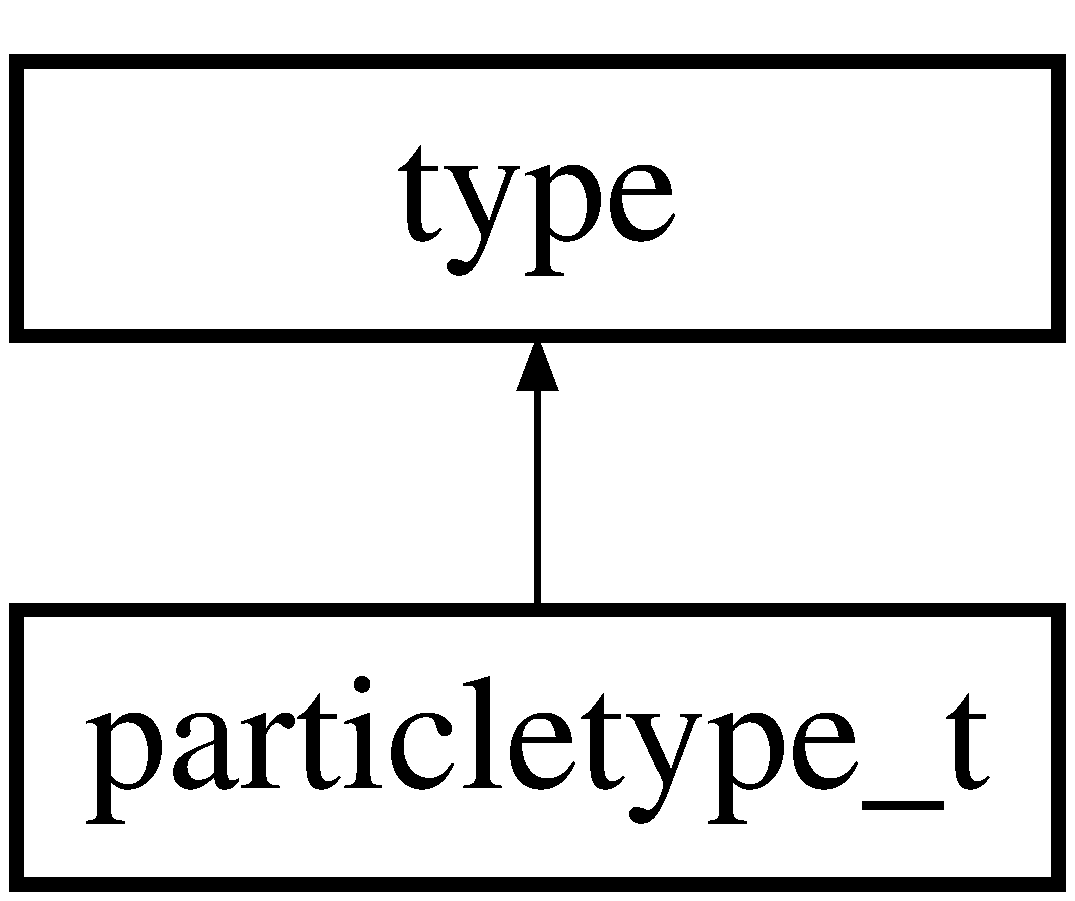
\includegraphics[height=2.000000cm]{classparticletype__t}
\end{center}
\end{figure}
\subsection*{Public Types}
\begin{DoxyCompactItemize}
\item 
typedef \+::\hyperlink{namespacexml__schema_acfa24ac68e1a188e7f44c36f7a158bf4}{xml\+\_\+schema\+::int\+\_\+} \hyperlink{classparticletype__t_af4592f0136ed3224434007bc7f5c7fd4}{id\+\_\+type}
\item 
typedef \+::xsd\+::cxx\+::tree\+::traits$<$ \hyperlink{classparticletype__t_af4592f0136ed3224434007bc7f5c7fd4}{id\+\_\+type}, char $>$ \hyperlink{classparticletype__t_ae11ed5b066a4f0eff6a0fd5c848242be}{id\+\_\+traits}
\item 
typedef \+::\hyperlink{namespacexml__schema_ad7e04ab17bba0b3fdde43fb79ef6ed87}{xml\+\_\+schema\+::float\+\_\+} \hyperlink{classparticletype__t_a7ebd18e57b545977bf3d1573ffa395f7}{mass\+\_\+type}
\item 
typedef \+::xsd\+::cxx\+::tree\+::traits$<$ \hyperlink{classparticletype__t_a7ebd18e57b545977bf3d1573ffa395f7}{mass\+\_\+type}, char $>$ \hyperlink{classparticletype__t_ac0e07de539bf88441c980a15bb88e1c9}{mass\+\_\+traits}
\item 
typedef \+::\hyperlink{namespacexml__schema_ad7e04ab17bba0b3fdde43fb79ef6ed87}{xml\+\_\+schema\+::float\+\_\+} \hyperlink{classparticletype__t_abbac1ed447872eb2db5cc90f2c1e1a6c}{sigma\+\_\+type}
\item 
typedef \+::xsd\+::cxx\+::tree\+::traits$<$ \hyperlink{classparticletype__t_abbac1ed447872eb2db5cc90f2c1e1a6c}{sigma\+\_\+type}, char $>$ \hyperlink{classparticletype__t_aa2caef2ce2ef568f535961d3ab84df2a}{sigma\+\_\+traits}
\item 
typedef \+::\hyperlink{namespacexml__schema_ad7e04ab17bba0b3fdde43fb79ef6ed87}{xml\+\_\+schema\+::float\+\_\+} \hyperlink{classparticletype__t_a94692265645066b820b0e4c308c1566f}{epsilon\+\_\+type}
\item 
typedef \+::xsd\+::cxx\+::tree\+::traits$<$ \hyperlink{classparticletype__t_a94692265645066b820b0e4c308c1566f}{epsilon\+\_\+type}, char $>$ \hyperlink{classparticletype__t_aba72bd9fc1660ca66d7294ea79e6a32e}{epsilon\+\_\+traits}
\item 
typedef \+::\hyperlink{namespacexml__schema_ae5ada4ec9c54b51765c3e4c0e9631bba}{xml\+\_\+schema\+::boolean} \hyperlink{classparticletype__t_a689bb940332f300e99acdf3d50ffdc2c}{fixed\+\_\+type}
\item 
typedef \+::xsd\+::cxx\+::tree\+::optional$<$ \hyperlink{classparticletype__t_a689bb940332f300e99acdf3d50ffdc2c}{fixed\+\_\+type} $>$ \hyperlink{classparticletype__t_a42eca3b383084472937b0ad4f370bbb2}{fixed\+\_\+optional}
\item 
typedef \+::xsd\+::cxx\+::tree\+::traits$<$ \hyperlink{classparticletype__t_a689bb940332f300e99acdf3d50ffdc2c}{fixed\+\_\+type}, char $>$ \hyperlink{classparticletype__t_ae90f4fb144ba140e553d5aaeca48ebb5}{fixed\+\_\+traits}
\item 
typedef \+::\hyperlink{namespacexml__schema_aac2d3d3483d3a20e8d96d2e8e5b3a470}{xml\+\_\+schema\+::double\+\_\+} \hyperlink{classparticletype__t_a3cd2c72b9a4607fb4e7022af7f979d61}{Rtrunc\+L\+J\+\_\+type}
\item 
typedef \+::xsd\+::cxx\+::tree\+::optional$<$ \hyperlink{classparticletype__t_a3cd2c72b9a4607fb4e7022af7f979d61}{Rtrunc\+L\+J\+\_\+type} $>$ \hyperlink{classparticletype__t_aa09967796541d58a44dfec6bcbb2c431}{Rtrunc\+L\+J\+\_\+optional}
\item 
typedef \+::xsd\+::cxx\+::tree\+::traits$<$ \hyperlink{classparticletype__t_a3cd2c72b9a4607fb4e7022af7f979d61}{Rtrunc\+L\+J\+\_\+type}, char,\+::xsd\+::cxx\+::tree\+::schema\+\_\+type\+::double\+\_\+ $>$ \hyperlink{classparticletype__t_acbef1d01c89e1d6db8eed5d7b7b8575c}{Rtrunc\+L\+J\+\_\+traits}
\end{DoxyCompactItemize}
\subsection*{Public Member Functions}
\begin{DoxyCompactItemize}
\item 
const \hyperlink{classparticletype__t_af4592f0136ed3224434007bc7f5c7fd4}{id\+\_\+type} \& \hyperlink{classparticletype__t_a17881ffeb3dd93830d1b33df6e17598a}{id} () const 
\item 
\hyperlink{classparticletype__t_af4592f0136ed3224434007bc7f5c7fd4}{id\+\_\+type} \& \hyperlink{classparticletype__t_acde6cba736f743c849306febf483e545}{id} ()
\item 
void \hyperlink{classparticletype__t_a4ecb8378ecc012687da000750fdb8d5c}{id} (const \hyperlink{classparticletype__t_af4592f0136ed3224434007bc7f5c7fd4}{id\+\_\+type} \&x)
\item 
const \hyperlink{classparticletype__t_a7ebd18e57b545977bf3d1573ffa395f7}{mass\+\_\+type} \& \hyperlink{classparticletype__t_a7b233c4a0330ede6dcdfb8ddeeebb9e0}{mass} () const 
\item 
\hyperlink{classparticletype__t_a7ebd18e57b545977bf3d1573ffa395f7}{mass\+\_\+type} \& \hyperlink{classparticletype__t_a4adcf91cc5576fd01523b709bb402ffa}{mass} ()
\item 
void \hyperlink{classparticletype__t_ab753b2e5c12a142f8b4cc07dabeaffcd}{mass} (const \hyperlink{classparticletype__t_a7ebd18e57b545977bf3d1573ffa395f7}{mass\+\_\+type} \&x)
\item 
const \hyperlink{classparticletype__t_abbac1ed447872eb2db5cc90f2c1e1a6c}{sigma\+\_\+type} \& \hyperlink{classparticletype__t_aa9189c46367b6c479fc70af923fe854b}{sigma} () const 
\item 
\hyperlink{classparticletype__t_abbac1ed447872eb2db5cc90f2c1e1a6c}{sigma\+\_\+type} \& \hyperlink{classparticletype__t_a399c3fbc49476267096288e440b3ab8b}{sigma} ()
\item 
void \hyperlink{classparticletype__t_a9d6b1333dc57e251dcb18056e7ec50b5}{sigma} (const \hyperlink{classparticletype__t_abbac1ed447872eb2db5cc90f2c1e1a6c}{sigma\+\_\+type} \&x)
\item 
const \hyperlink{classparticletype__t_a94692265645066b820b0e4c308c1566f}{epsilon\+\_\+type} \& \hyperlink{classparticletype__t_a59a6eafceba5dfb7628544e655a75878}{epsilon} () const 
\item 
\hyperlink{classparticletype__t_a94692265645066b820b0e4c308c1566f}{epsilon\+\_\+type} \& \hyperlink{classparticletype__t_ae8bc5195d983bacb82dd04f96f14097c}{epsilon} ()
\item 
void \hyperlink{classparticletype__t_abdba8823cb3cf31e884108daf55e8c68}{epsilon} (const \hyperlink{classparticletype__t_a94692265645066b820b0e4c308c1566f}{epsilon\+\_\+type} \&x)
\item 
const \hyperlink{classparticletype__t_a42eca3b383084472937b0ad4f370bbb2}{fixed\+\_\+optional} \& \hyperlink{classparticletype__t_a769f7e73caa39b4053eebae6a63b1bb0}{fixed} () const 
\item 
\hyperlink{classparticletype__t_a42eca3b383084472937b0ad4f370bbb2}{fixed\+\_\+optional} \& \hyperlink{classparticletype__t_a28426e8b4befda5b7a23aa4bb8e0eaee}{fixed} ()
\item 
void \hyperlink{classparticletype__t_a91eb27766f83482598408c6037d98ade}{fixed} (const \hyperlink{classparticletype__t_a689bb940332f300e99acdf3d50ffdc2c}{fixed\+\_\+type} \&x)
\item 
void \hyperlink{classparticletype__t_aa28d598502ab069d15b393a4c7cc2cf4}{fixed} (const \hyperlink{classparticletype__t_a42eca3b383084472937b0ad4f370bbb2}{fixed\+\_\+optional} \&x)
\item 
const \hyperlink{classparticletype__t_aa09967796541d58a44dfec6bcbb2c431}{Rtrunc\+L\+J\+\_\+optional} \& \hyperlink{classparticletype__t_a12397bd11e44dff87e3af98935cd177a}{Rtrunc\+LJ} () const 
\item 
\hyperlink{classparticletype__t_aa09967796541d58a44dfec6bcbb2c431}{Rtrunc\+L\+J\+\_\+optional} \& \hyperlink{classparticletype__t_a6189394520c9d7491e84c86a73c24969}{Rtrunc\+LJ} ()
\item 
void \hyperlink{classparticletype__t_a3a7d8c317728cbafed77153720c49f21}{Rtrunc\+LJ} (const \hyperlink{classparticletype__t_a3cd2c72b9a4607fb4e7022af7f979d61}{Rtrunc\+L\+J\+\_\+type} \&x)
\item 
void \hyperlink{classparticletype__t_a2e0c97e6c6c53b81c9ee52b598efe084}{Rtrunc\+LJ} (const \hyperlink{classparticletype__t_aa09967796541d58a44dfec6bcbb2c431}{Rtrunc\+L\+J\+\_\+optional} \&x)
\item 
\hyperlink{classparticletype__t_a9b7f4ea289cabc2ed87162ba7ac57236}{particletype\+\_\+t} (const \hyperlink{classparticletype__t_af4592f0136ed3224434007bc7f5c7fd4}{id\+\_\+type} \&, const \hyperlink{classparticletype__t_a7ebd18e57b545977bf3d1573ffa395f7}{mass\+\_\+type} \&, const \hyperlink{classparticletype__t_abbac1ed447872eb2db5cc90f2c1e1a6c}{sigma\+\_\+type} \&, const \hyperlink{classparticletype__t_a94692265645066b820b0e4c308c1566f}{epsilon\+\_\+type} \&)
\item 
\hyperlink{classparticletype__t_a580bd1128ee7796c9b2ec9f463f91b5b}{particletype\+\_\+t} (const \+::xercesc\+::\+D\+O\+M\+Element \&e,\+::\hyperlink{namespacexml__schema_a0612287d030cb2732d31a45b258fdc87}{xml\+\_\+schema\+::flags} f=0,\+::\hyperlink{namespacexml__schema_ada9aa30dc722e93ee2ed7243085402a5}{xml\+\_\+schema\+::container} $\ast$c=0)
\item 
\hyperlink{classparticletype__t_a86329e35b2ba5ca62f63ffa0b5743dc2}{particletype\+\_\+t} (const \hyperlink{classparticletype__t}{particletype\+\_\+t} \&x,\+::\hyperlink{namespacexml__schema_a0612287d030cb2732d31a45b258fdc87}{xml\+\_\+schema\+::flags} f=0,\+::\hyperlink{namespacexml__schema_ada9aa30dc722e93ee2ed7243085402a5}{xml\+\_\+schema\+::container} $\ast$c=0)
\item 
virtual \hyperlink{classparticletype__t}{particletype\+\_\+t} $\ast$ \hyperlink{classparticletype__t_a17d289547d6936235e99c04a08baa9ad}{\+\_\+clone} (\+::\hyperlink{namespacexml__schema_a0612287d030cb2732d31a45b258fdc87}{xml\+\_\+schema\+::flags} f=0,\+::\hyperlink{namespacexml__schema_ada9aa30dc722e93ee2ed7243085402a5}{xml\+\_\+schema\+::container} $\ast$c=0) const 
\item 
\hyperlink{classparticletype__t}{particletype\+\_\+t} \& \hyperlink{classparticletype__t_a34e937edde9d73aa411c175182e6006a}{operator=} (const \hyperlink{classparticletype__t}{particletype\+\_\+t} \&x)
\item 
virtual \hyperlink{classparticletype__t_aa5a6a6252899d8263b91b4e098969c2d}{$\sim$particletype\+\_\+t} ()
\end{DoxyCompactItemize}
\subsection*{Protected Member Functions}
\begin{DoxyCompactItemize}
\item 
void \hyperlink{classparticletype__t_a7a353632a13af1c190a9fb5cafa6bd36}{parse} (\+::xsd\+::cxx\+::xml\+::dom\+::parser$<$ char $>$ \&,\+::\hyperlink{namespacexml__schema_a0612287d030cb2732d31a45b258fdc87}{xml\+\_\+schema\+::flags})
\end{DoxyCompactItemize}
\subsection*{Protected Attributes}
\begin{DoxyCompactItemize}
\item 
\+::xsd\+::cxx\+::tree\+::one$<$ \hyperlink{classparticletype__t_af4592f0136ed3224434007bc7f5c7fd4}{id\+\_\+type} $>$ \hyperlink{classparticletype__t_a14b4df24e40439bf766545034eb33256}{id\+\_\+}
\item 
\+::xsd\+::cxx\+::tree\+::one$<$ \hyperlink{classparticletype__t_a7ebd18e57b545977bf3d1573ffa395f7}{mass\+\_\+type} $>$ \hyperlink{classparticletype__t_a833425b7549845017f4f53201e261c76}{mass\+\_\+}
\item 
\+::xsd\+::cxx\+::tree\+::one$<$ \hyperlink{classparticletype__t_abbac1ed447872eb2db5cc90f2c1e1a6c}{sigma\+\_\+type} $>$ \hyperlink{classparticletype__t_a1d31f582a032e178f3e0832a7202fa68}{sigma\+\_\+}
\item 
\+::xsd\+::cxx\+::tree\+::one$<$ \hyperlink{classparticletype__t_a94692265645066b820b0e4c308c1566f}{epsilon\+\_\+type} $>$ \hyperlink{classparticletype__t_a2ab316a2ae4738c32883b046924c5aea}{epsilon\+\_\+}
\item 
\hyperlink{classparticletype__t_a42eca3b383084472937b0ad4f370bbb2}{fixed\+\_\+optional} \hyperlink{classparticletype__t_a81af477c09b255cac4d1fd909a7541dd}{fixed\+\_\+}
\item 
\hyperlink{classparticletype__t_aa09967796541d58a44dfec6bcbb2c431}{Rtrunc\+L\+J\+\_\+optional} \hyperlink{classparticletype__t_ae0011fe9477c7239e4e270378ea1ddbc}{Rtrunc\+L\+J\+\_\+}
\end{DoxyCompactItemize}


\subsection{Member Typedef Documentation}
\index{particletype\+\_\+t@{particletype\+\_\+t}!epsilon\+\_\+traits@{epsilon\+\_\+traits}}
\index{epsilon\+\_\+traits@{epsilon\+\_\+traits}!particletype\+\_\+t@{particletype\+\_\+t}}
\subsubsection[{\texorpdfstring{epsilon\+\_\+traits}{epsilon_traits}}]{\setlength{\rightskip}{0pt plus 5cm}typedef \+::xsd\+::cxx\+::tree\+::traits$<$ {\bf epsilon\+\_\+type}, char $>$ {\bf particletype\+\_\+t\+::epsilon\+\_\+traits}}\hypertarget{classparticletype__t_aba72bd9fc1660ca66d7294ea79e6a32e}{}\label{classparticletype__t_aba72bd9fc1660ca66d7294ea79e6a32e}
\index{particletype\+\_\+t@{particletype\+\_\+t}!epsilon\+\_\+type@{epsilon\+\_\+type}}
\index{epsilon\+\_\+type@{epsilon\+\_\+type}!particletype\+\_\+t@{particletype\+\_\+t}}
\subsubsection[{\texorpdfstring{epsilon\+\_\+type}{epsilon_type}}]{\setlength{\rightskip}{0pt plus 5cm}typedef \+::{\bf xml\+\_\+schema\+::float\+\_\+} {\bf particletype\+\_\+t\+::epsilon\+\_\+type}}\hypertarget{classparticletype__t_a94692265645066b820b0e4c308c1566f}{}\label{classparticletype__t_a94692265645066b820b0e4c308c1566f}
\index{particletype\+\_\+t@{particletype\+\_\+t}!fixed\+\_\+optional@{fixed\+\_\+optional}}
\index{fixed\+\_\+optional@{fixed\+\_\+optional}!particletype\+\_\+t@{particletype\+\_\+t}}
\subsubsection[{\texorpdfstring{fixed\+\_\+optional}{fixed_optional}}]{\setlength{\rightskip}{0pt plus 5cm}typedef \+::xsd\+::cxx\+::tree\+::optional$<$ {\bf fixed\+\_\+type} $>$ {\bf particletype\+\_\+t\+::fixed\+\_\+optional}}\hypertarget{classparticletype__t_a42eca3b383084472937b0ad4f370bbb2}{}\label{classparticletype__t_a42eca3b383084472937b0ad4f370bbb2}
\index{particletype\+\_\+t@{particletype\+\_\+t}!fixed\+\_\+traits@{fixed\+\_\+traits}}
\index{fixed\+\_\+traits@{fixed\+\_\+traits}!particletype\+\_\+t@{particletype\+\_\+t}}
\subsubsection[{\texorpdfstring{fixed\+\_\+traits}{fixed_traits}}]{\setlength{\rightskip}{0pt plus 5cm}typedef \+::xsd\+::cxx\+::tree\+::traits$<$ {\bf fixed\+\_\+type}, char $>$ {\bf particletype\+\_\+t\+::fixed\+\_\+traits}}\hypertarget{classparticletype__t_ae90f4fb144ba140e553d5aaeca48ebb5}{}\label{classparticletype__t_ae90f4fb144ba140e553d5aaeca48ebb5}
\index{particletype\+\_\+t@{particletype\+\_\+t}!fixed\+\_\+type@{fixed\+\_\+type}}
\index{fixed\+\_\+type@{fixed\+\_\+type}!particletype\+\_\+t@{particletype\+\_\+t}}
\subsubsection[{\texorpdfstring{fixed\+\_\+type}{fixed_type}}]{\setlength{\rightskip}{0pt plus 5cm}typedef \+::{\bf xml\+\_\+schema\+::boolean} {\bf particletype\+\_\+t\+::fixed\+\_\+type}}\hypertarget{classparticletype__t_a689bb940332f300e99acdf3d50ffdc2c}{}\label{classparticletype__t_a689bb940332f300e99acdf3d50ffdc2c}
\index{particletype\+\_\+t@{particletype\+\_\+t}!id\+\_\+traits@{id\+\_\+traits}}
\index{id\+\_\+traits@{id\+\_\+traits}!particletype\+\_\+t@{particletype\+\_\+t}}
\subsubsection[{\texorpdfstring{id\+\_\+traits}{id_traits}}]{\setlength{\rightskip}{0pt plus 5cm}typedef \+::xsd\+::cxx\+::tree\+::traits$<$ {\bf id\+\_\+type}, char $>$ {\bf particletype\+\_\+t\+::id\+\_\+traits}}\hypertarget{classparticletype__t_ae11ed5b066a4f0eff6a0fd5c848242be}{}\label{classparticletype__t_ae11ed5b066a4f0eff6a0fd5c848242be}
\index{particletype\+\_\+t@{particletype\+\_\+t}!id\+\_\+type@{id\+\_\+type}}
\index{id\+\_\+type@{id\+\_\+type}!particletype\+\_\+t@{particletype\+\_\+t}}
\subsubsection[{\texorpdfstring{id\+\_\+type}{id_type}}]{\setlength{\rightskip}{0pt plus 5cm}typedef \+::{\bf xml\+\_\+schema\+::int\+\_\+} {\bf particletype\+\_\+t\+::id\+\_\+type}}\hypertarget{classparticletype__t_af4592f0136ed3224434007bc7f5c7fd4}{}\label{classparticletype__t_af4592f0136ed3224434007bc7f5c7fd4}
\index{particletype\+\_\+t@{particletype\+\_\+t}!mass\+\_\+traits@{mass\+\_\+traits}}
\index{mass\+\_\+traits@{mass\+\_\+traits}!particletype\+\_\+t@{particletype\+\_\+t}}
\subsubsection[{\texorpdfstring{mass\+\_\+traits}{mass_traits}}]{\setlength{\rightskip}{0pt plus 5cm}typedef \+::xsd\+::cxx\+::tree\+::traits$<$ {\bf mass\+\_\+type}, char $>$ {\bf particletype\+\_\+t\+::mass\+\_\+traits}}\hypertarget{classparticletype__t_ac0e07de539bf88441c980a15bb88e1c9}{}\label{classparticletype__t_ac0e07de539bf88441c980a15bb88e1c9}
\index{particletype\+\_\+t@{particletype\+\_\+t}!mass\+\_\+type@{mass\+\_\+type}}
\index{mass\+\_\+type@{mass\+\_\+type}!particletype\+\_\+t@{particletype\+\_\+t}}
\subsubsection[{\texorpdfstring{mass\+\_\+type}{mass_type}}]{\setlength{\rightskip}{0pt plus 5cm}typedef \+::{\bf xml\+\_\+schema\+::float\+\_\+} {\bf particletype\+\_\+t\+::mass\+\_\+type}}\hypertarget{classparticletype__t_a7ebd18e57b545977bf3d1573ffa395f7}{}\label{classparticletype__t_a7ebd18e57b545977bf3d1573ffa395f7}
\index{particletype\+\_\+t@{particletype\+\_\+t}!Rtrunc\+L\+J\+\_\+optional@{Rtrunc\+L\+J\+\_\+optional}}
\index{Rtrunc\+L\+J\+\_\+optional@{Rtrunc\+L\+J\+\_\+optional}!particletype\+\_\+t@{particletype\+\_\+t}}
\subsubsection[{\texorpdfstring{Rtrunc\+L\+J\+\_\+optional}{RtruncLJ_optional}}]{\setlength{\rightskip}{0pt plus 5cm}typedef \+::xsd\+::cxx\+::tree\+::optional$<$ {\bf Rtrunc\+L\+J\+\_\+type} $>$ {\bf particletype\+\_\+t\+::\+Rtrunc\+L\+J\+\_\+optional}}\hypertarget{classparticletype__t_aa09967796541d58a44dfec6bcbb2c431}{}\label{classparticletype__t_aa09967796541d58a44dfec6bcbb2c431}
\index{particletype\+\_\+t@{particletype\+\_\+t}!Rtrunc\+L\+J\+\_\+traits@{Rtrunc\+L\+J\+\_\+traits}}
\index{Rtrunc\+L\+J\+\_\+traits@{Rtrunc\+L\+J\+\_\+traits}!particletype\+\_\+t@{particletype\+\_\+t}}
\subsubsection[{\texorpdfstring{Rtrunc\+L\+J\+\_\+traits}{RtruncLJ_traits}}]{\setlength{\rightskip}{0pt plus 5cm}typedef \+::xsd\+::cxx\+::tree\+::traits$<$ {\bf Rtrunc\+L\+J\+\_\+type}, char, \+::xsd\+::cxx\+::tree\+::schema\+\_\+type\+::double\+\_\+ $>$ {\bf particletype\+\_\+t\+::\+Rtrunc\+L\+J\+\_\+traits}}\hypertarget{classparticletype__t_acbef1d01c89e1d6db8eed5d7b7b8575c}{}\label{classparticletype__t_acbef1d01c89e1d6db8eed5d7b7b8575c}
\index{particletype\+\_\+t@{particletype\+\_\+t}!Rtrunc\+L\+J\+\_\+type@{Rtrunc\+L\+J\+\_\+type}}
\index{Rtrunc\+L\+J\+\_\+type@{Rtrunc\+L\+J\+\_\+type}!particletype\+\_\+t@{particletype\+\_\+t}}
\subsubsection[{\texorpdfstring{Rtrunc\+L\+J\+\_\+type}{RtruncLJ_type}}]{\setlength{\rightskip}{0pt plus 5cm}typedef \+::{\bf xml\+\_\+schema\+::double\+\_\+} {\bf particletype\+\_\+t\+::\+Rtrunc\+L\+J\+\_\+type}}\hypertarget{classparticletype__t_a3cd2c72b9a4607fb4e7022af7f979d61}{}\label{classparticletype__t_a3cd2c72b9a4607fb4e7022af7f979d61}
\index{particletype\+\_\+t@{particletype\+\_\+t}!sigma\+\_\+traits@{sigma\+\_\+traits}}
\index{sigma\+\_\+traits@{sigma\+\_\+traits}!particletype\+\_\+t@{particletype\+\_\+t}}
\subsubsection[{\texorpdfstring{sigma\+\_\+traits}{sigma_traits}}]{\setlength{\rightskip}{0pt plus 5cm}typedef \+::xsd\+::cxx\+::tree\+::traits$<$ {\bf sigma\+\_\+type}, char $>$ {\bf particletype\+\_\+t\+::sigma\+\_\+traits}}\hypertarget{classparticletype__t_aa2caef2ce2ef568f535961d3ab84df2a}{}\label{classparticletype__t_aa2caef2ce2ef568f535961d3ab84df2a}
\index{particletype\+\_\+t@{particletype\+\_\+t}!sigma\+\_\+type@{sigma\+\_\+type}}
\index{sigma\+\_\+type@{sigma\+\_\+type}!particletype\+\_\+t@{particletype\+\_\+t}}
\subsubsection[{\texorpdfstring{sigma\+\_\+type}{sigma_type}}]{\setlength{\rightskip}{0pt plus 5cm}typedef \+::{\bf xml\+\_\+schema\+::float\+\_\+} {\bf particletype\+\_\+t\+::sigma\+\_\+type}}\hypertarget{classparticletype__t_abbac1ed447872eb2db5cc90f2c1e1a6c}{}\label{classparticletype__t_abbac1ed447872eb2db5cc90f2c1e1a6c}


\subsection{Constructor \& Destructor Documentation}
\index{particletype\+\_\+t@{particletype\+\_\+t}!particletype\+\_\+t@{particletype\+\_\+t}}
\index{particletype\+\_\+t@{particletype\+\_\+t}!particletype\+\_\+t@{particletype\+\_\+t}}
\subsubsection[{\texorpdfstring{particletype\+\_\+t(const id\+\_\+type \&, const mass\+\_\+type \&, const sigma\+\_\+type \&, const epsilon\+\_\+type \&)}{particletype_t(const id_type &, const mass_type &, const sigma_type &, const epsilon_type &)}}]{\setlength{\rightskip}{0pt plus 5cm}particletype\+\_\+t\+::particletype\+\_\+t (
\begin{DoxyParamCaption}
\item[{const {\bf id\+\_\+type} \&}]{id, }
\item[{const {\bf mass\+\_\+type} \&}]{mass, }
\item[{const {\bf sigma\+\_\+type} \&}]{sigma, }
\item[{const {\bf epsilon\+\_\+type} \&}]{epsilon}
\end{DoxyParamCaption}
)}\hypertarget{classparticletype__t_a9b7f4ea289cabc2ed87162ba7ac57236}{}\label{classparticletype__t_a9b7f4ea289cabc2ed87162ba7ac57236}
\index{particletype\+\_\+t@{particletype\+\_\+t}!particletype\+\_\+t@{particletype\+\_\+t}}
\index{particletype\+\_\+t@{particletype\+\_\+t}!particletype\+\_\+t@{particletype\+\_\+t}}
\subsubsection[{\texorpdfstring{particletype\+\_\+t(const \+::xercesc\+::\+D\+O\+M\+Element \&e,\+::xml\+\_\+schema\+::flags f=0,\+::xml\+\_\+schema\+::container $\ast$c=0)}{particletype_t(const ::xercesc::DOMElement &e,::xml_schema::flags f=0,::xml_schema::container *c=0)}}]{\setlength{\rightskip}{0pt plus 5cm}particletype\+\_\+t\+::particletype\+\_\+t (
\begin{DoxyParamCaption}
\item[{const \+::xercesc\+::\+D\+O\+M\+Element \&}]{e, }
\item[{\+::{\bf xml\+\_\+schema\+::flags}}]{f = {\ttfamily 0}, }
\item[{\+::{\bf xml\+\_\+schema\+::container} $\ast$}]{c = {\ttfamily 0}}
\end{DoxyParamCaption}
)}\hypertarget{classparticletype__t_a580bd1128ee7796c9b2ec9f463f91b5b}{}\label{classparticletype__t_a580bd1128ee7796c9b2ec9f463f91b5b}
\index{particletype\+\_\+t@{particletype\+\_\+t}!particletype\+\_\+t@{particletype\+\_\+t}}
\index{particletype\+\_\+t@{particletype\+\_\+t}!particletype\+\_\+t@{particletype\+\_\+t}}
\subsubsection[{\texorpdfstring{particletype\+\_\+t(const particletype\+\_\+t \&x,\+::xml\+\_\+schema\+::flags f=0,\+::xml\+\_\+schema\+::container $\ast$c=0)}{particletype_t(const particletype_t &x,::xml_schema::flags f=0,::xml_schema::container *c=0)}}]{\setlength{\rightskip}{0pt plus 5cm}particletype\+\_\+t\+::particletype\+\_\+t (
\begin{DoxyParamCaption}
\item[{const {\bf particletype\+\_\+t} \&}]{x, }
\item[{\+::{\bf xml\+\_\+schema\+::flags}}]{f = {\ttfamily 0}, }
\item[{\+::{\bf xml\+\_\+schema\+::container} $\ast$}]{c = {\ttfamily 0}}
\end{DoxyParamCaption}
)}\hypertarget{classparticletype__t_a86329e35b2ba5ca62f63ffa0b5743dc2}{}\label{classparticletype__t_a86329e35b2ba5ca62f63ffa0b5743dc2}
\index{particletype\+\_\+t@{particletype\+\_\+t}!````~particletype\+\_\+t@{$\sim$particletype\+\_\+t}}
\index{````~particletype\+\_\+t@{$\sim$particletype\+\_\+t}!particletype\+\_\+t@{particletype\+\_\+t}}
\subsubsection[{\texorpdfstring{$\sim$particletype\+\_\+t()}{~particletype_t()}}]{\setlength{\rightskip}{0pt plus 5cm}particletype\+\_\+t\+::$\sim$particletype\+\_\+t (
\begin{DoxyParamCaption}
{}
\end{DoxyParamCaption}
)\hspace{0.3cm}{\ttfamily [virtual]}}\hypertarget{classparticletype__t_aa5a6a6252899d8263b91b4e098969c2d}{}\label{classparticletype__t_aa5a6a6252899d8263b91b4e098969c2d}


\subsection{Member Function Documentation}
\index{particletype\+\_\+t@{particletype\+\_\+t}!\+\_\+clone@{\+\_\+clone}}
\index{\+\_\+clone@{\+\_\+clone}!particletype\+\_\+t@{particletype\+\_\+t}}
\subsubsection[{\texorpdfstring{\+\_\+clone(\+::xml\+\_\+schema\+::flags f=0,\+::xml\+\_\+schema\+::container $\ast$c=0) const }{_clone(::xml_schema::flags f=0,::xml_schema::container *c=0) const }}]{\setlength{\rightskip}{0pt plus 5cm}{\bf particletype\+\_\+t} $\ast$ particletype\+\_\+t\+::\+\_\+clone (
\begin{DoxyParamCaption}
\item[{\+::{\bf xml\+\_\+schema\+::flags}}]{f = {\ttfamily 0}, }
\item[{\+::{\bf xml\+\_\+schema\+::container} $\ast$}]{c = {\ttfamily 0}}
\end{DoxyParamCaption}
) const\hspace{0.3cm}{\ttfamily [virtual]}}\hypertarget{classparticletype__t_a17d289547d6936235e99c04a08baa9ad}{}\label{classparticletype__t_a17d289547d6936235e99c04a08baa9ad}
\index{particletype\+\_\+t@{particletype\+\_\+t}!epsilon@{epsilon}}
\index{epsilon@{epsilon}!particletype\+\_\+t@{particletype\+\_\+t}}
\subsubsection[{\texorpdfstring{epsilon() const }{epsilon() const }}]{\setlength{\rightskip}{0pt plus 5cm}const {\bf particletype\+\_\+t\+::epsilon\+\_\+type} \& particletype\+\_\+t\+::epsilon (
\begin{DoxyParamCaption}
{}
\end{DoxyParamCaption}
) const}\hypertarget{classparticletype__t_a59a6eafceba5dfb7628544e655a75878}{}\label{classparticletype__t_a59a6eafceba5dfb7628544e655a75878}
\index{particletype\+\_\+t@{particletype\+\_\+t}!epsilon@{epsilon}}
\index{epsilon@{epsilon}!particletype\+\_\+t@{particletype\+\_\+t}}
\subsubsection[{\texorpdfstring{epsilon()}{epsilon()}}]{\setlength{\rightskip}{0pt plus 5cm}{\bf particletype\+\_\+t\+::epsilon\+\_\+type} \& particletype\+\_\+t\+::epsilon (
\begin{DoxyParamCaption}
{}
\end{DoxyParamCaption}
)}\hypertarget{classparticletype__t_ae8bc5195d983bacb82dd04f96f14097c}{}\label{classparticletype__t_ae8bc5195d983bacb82dd04f96f14097c}
\index{particletype\+\_\+t@{particletype\+\_\+t}!epsilon@{epsilon}}
\index{epsilon@{epsilon}!particletype\+\_\+t@{particletype\+\_\+t}}
\subsubsection[{\texorpdfstring{epsilon(const epsilon\+\_\+type \&x)}{epsilon(const epsilon_type &x)}}]{\setlength{\rightskip}{0pt plus 5cm}void particletype\+\_\+t\+::epsilon (
\begin{DoxyParamCaption}
\item[{const {\bf epsilon\+\_\+type} \&}]{x}
\end{DoxyParamCaption}
)}\hypertarget{classparticletype__t_abdba8823cb3cf31e884108daf55e8c68}{}\label{classparticletype__t_abdba8823cb3cf31e884108daf55e8c68}
\index{particletype\+\_\+t@{particletype\+\_\+t}!fixed@{fixed}}
\index{fixed@{fixed}!particletype\+\_\+t@{particletype\+\_\+t}}
\subsubsection[{\texorpdfstring{fixed() const }{fixed() const }}]{\setlength{\rightskip}{0pt plus 5cm}const {\bf particletype\+\_\+t\+::fixed\+\_\+optional} \& particletype\+\_\+t\+::fixed (
\begin{DoxyParamCaption}
{}
\end{DoxyParamCaption}
) const}\hypertarget{classparticletype__t_a769f7e73caa39b4053eebae6a63b1bb0}{}\label{classparticletype__t_a769f7e73caa39b4053eebae6a63b1bb0}
\index{particletype\+\_\+t@{particletype\+\_\+t}!fixed@{fixed}}
\index{fixed@{fixed}!particletype\+\_\+t@{particletype\+\_\+t}}
\subsubsection[{\texorpdfstring{fixed()}{fixed()}}]{\setlength{\rightskip}{0pt plus 5cm}{\bf particletype\+\_\+t\+::fixed\+\_\+optional} \& particletype\+\_\+t\+::fixed (
\begin{DoxyParamCaption}
{}
\end{DoxyParamCaption}
)}\hypertarget{classparticletype__t_a28426e8b4befda5b7a23aa4bb8e0eaee}{}\label{classparticletype__t_a28426e8b4befda5b7a23aa4bb8e0eaee}
\index{particletype\+\_\+t@{particletype\+\_\+t}!fixed@{fixed}}
\index{fixed@{fixed}!particletype\+\_\+t@{particletype\+\_\+t}}
\subsubsection[{\texorpdfstring{fixed(const fixed\+\_\+type \&x)}{fixed(const fixed_type &x)}}]{\setlength{\rightskip}{0pt plus 5cm}void particletype\+\_\+t\+::fixed (
\begin{DoxyParamCaption}
\item[{const {\bf fixed\+\_\+type} \&}]{x}
\end{DoxyParamCaption}
)}\hypertarget{classparticletype__t_a91eb27766f83482598408c6037d98ade}{}\label{classparticletype__t_a91eb27766f83482598408c6037d98ade}
\index{particletype\+\_\+t@{particletype\+\_\+t}!fixed@{fixed}}
\index{fixed@{fixed}!particletype\+\_\+t@{particletype\+\_\+t}}
\subsubsection[{\texorpdfstring{fixed(const fixed\+\_\+optional \&x)}{fixed(const fixed_optional &x)}}]{\setlength{\rightskip}{0pt plus 5cm}void particletype\+\_\+t\+::fixed (
\begin{DoxyParamCaption}
\item[{const {\bf fixed\+\_\+optional} \&}]{x}
\end{DoxyParamCaption}
)}\hypertarget{classparticletype__t_aa28d598502ab069d15b393a4c7cc2cf4}{}\label{classparticletype__t_aa28d598502ab069d15b393a4c7cc2cf4}
\index{particletype\+\_\+t@{particletype\+\_\+t}!id@{id}}
\index{id@{id}!particletype\+\_\+t@{particletype\+\_\+t}}
\subsubsection[{\texorpdfstring{id() const }{id() const }}]{\setlength{\rightskip}{0pt plus 5cm}const {\bf particletype\+\_\+t\+::id\+\_\+type} \& particletype\+\_\+t\+::id (
\begin{DoxyParamCaption}
{}
\end{DoxyParamCaption}
) const}\hypertarget{classparticletype__t_a17881ffeb3dd93830d1b33df6e17598a}{}\label{classparticletype__t_a17881ffeb3dd93830d1b33df6e17598a}
\index{particletype\+\_\+t@{particletype\+\_\+t}!id@{id}}
\index{id@{id}!particletype\+\_\+t@{particletype\+\_\+t}}
\subsubsection[{\texorpdfstring{id()}{id()}}]{\setlength{\rightskip}{0pt plus 5cm}{\bf particletype\+\_\+t\+::id\+\_\+type} \& particletype\+\_\+t\+::id (
\begin{DoxyParamCaption}
{}
\end{DoxyParamCaption}
)}\hypertarget{classparticletype__t_acde6cba736f743c849306febf483e545}{}\label{classparticletype__t_acde6cba736f743c849306febf483e545}
\index{particletype\+\_\+t@{particletype\+\_\+t}!id@{id}}
\index{id@{id}!particletype\+\_\+t@{particletype\+\_\+t}}
\subsubsection[{\texorpdfstring{id(const id\+\_\+type \&x)}{id(const id_type &x)}}]{\setlength{\rightskip}{0pt plus 5cm}void particletype\+\_\+t\+::id (
\begin{DoxyParamCaption}
\item[{const {\bf id\+\_\+type} \&}]{x}
\end{DoxyParamCaption}
)}\hypertarget{classparticletype__t_a4ecb8378ecc012687da000750fdb8d5c}{}\label{classparticletype__t_a4ecb8378ecc012687da000750fdb8d5c}
\index{particletype\+\_\+t@{particletype\+\_\+t}!mass@{mass}}
\index{mass@{mass}!particletype\+\_\+t@{particletype\+\_\+t}}
\subsubsection[{\texorpdfstring{mass() const }{mass() const }}]{\setlength{\rightskip}{0pt plus 5cm}const {\bf particletype\+\_\+t\+::mass\+\_\+type} \& particletype\+\_\+t\+::mass (
\begin{DoxyParamCaption}
{}
\end{DoxyParamCaption}
) const}\hypertarget{classparticletype__t_a7b233c4a0330ede6dcdfb8ddeeebb9e0}{}\label{classparticletype__t_a7b233c4a0330ede6dcdfb8ddeeebb9e0}
\index{particletype\+\_\+t@{particletype\+\_\+t}!mass@{mass}}
\index{mass@{mass}!particletype\+\_\+t@{particletype\+\_\+t}}
\subsubsection[{\texorpdfstring{mass()}{mass()}}]{\setlength{\rightskip}{0pt plus 5cm}{\bf particletype\+\_\+t\+::mass\+\_\+type} \& particletype\+\_\+t\+::mass (
\begin{DoxyParamCaption}
{}
\end{DoxyParamCaption}
)}\hypertarget{classparticletype__t_a4adcf91cc5576fd01523b709bb402ffa}{}\label{classparticletype__t_a4adcf91cc5576fd01523b709bb402ffa}
\index{particletype\+\_\+t@{particletype\+\_\+t}!mass@{mass}}
\index{mass@{mass}!particletype\+\_\+t@{particletype\+\_\+t}}
\subsubsection[{\texorpdfstring{mass(const mass\+\_\+type \&x)}{mass(const mass_type &x)}}]{\setlength{\rightskip}{0pt plus 5cm}void particletype\+\_\+t\+::mass (
\begin{DoxyParamCaption}
\item[{const {\bf mass\+\_\+type} \&}]{x}
\end{DoxyParamCaption}
)}\hypertarget{classparticletype__t_ab753b2e5c12a142f8b4cc07dabeaffcd}{}\label{classparticletype__t_ab753b2e5c12a142f8b4cc07dabeaffcd}
\index{particletype\+\_\+t@{particletype\+\_\+t}!operator=@{operator=}}
\index{operator=@{operator=}!particletype\+\_\+t@{particletype\+\_\+t}}
\subsubsection[{\texorpdfstring{operator=(const particletype\+\_\+t \&x)}{operator=(const particletype_t &x)}}]{\setlength{\rightskip}{0pt plus 5cm}{\bf particletype\+\_\+t} \& particletype\+\_\+t\+::operator= (
\begin{DoxyParamCaption}
\item[{const {\bf particletype\+\_\+t} \&}]{x}
\end{DoxyParamCaption}
)}\hypertarget{classparticletype__t_a34e937edde9d73aa411c175182e6006a}{}\label{classparticletype__t_a34e937edde9d73aa411c175182e6006a}
\index{particletype\+\_\+t@{particletype\+\_\+t}!parse@{parse}}
\index{parse@{parse}!particletype\+\_\+t@{particletype\+\_\+t}}
\subsubsection[{\texorpdfstring{parse(\+::xsd\+::cxx\+::xml\+::dom\+::parser$<$ char $>$ \&,\+::xml\+\_\+schema\+::flags)}{parse(::xsd::cxx::xml::dom::parser< char > &,::xml_schema::flags)}}]{\setlength{\rightskip}{0pt plus 5cm}void particletype\+\_\+t\+::parse (
\begin{DoxyParamCaption}
\item[{\+::xsd\+::cxx\+::xml\+::dom\+::parser$<$ char $>$ \&}]{p, }
\item[{\+::{\bf xml\+\_\+schema\+::flags}}]{f}
\end{DoxyParamCaption}
)\hspace{0.3cm}{\ttfamily [protected]}}\hypertarget{classparticletype__t_a7a353632a13af1c190a9fb5cafa6bd36}{}\label{classparticletype__t_a7a353632a13af1c190a9fb5cafa6bd36}
\index{particletype\+\_\+t@{particletype\+\_\+t}!Rtrunc\+LJ@{Rtrunc\+LJ}}
\index{Rtrunc\+LJ@{Rtrunc\+LJ}!particletype\+\_\+t@{particletype\+\_\+t}}
\subsubsection[{\texorpdfstring{Rtrunc\+L\+J() const }{RtruncLJ() const }}]{\setlength{\rightskip}{0pt plus 5cm}const {\bf particletype\+\_\+t\+::\+Rtrunc\+L\+J\+\_\+optional} \& particletype\+\_\+t\+::\+Rtrunc\+LJ (
\begin{DoxyParamCaption}
{}
\end{DoxyParamCaption}
) const}\hypertarget{classparticletype__t_a12397bd11e44dff87e3af98935cd177a}{}\label{classparticletype__t_a12397bd11e44dff87e3af98935cd177a}
\index{particletype\+\_\+t@{particletype\+\_\+t}!Rtrunc\+LJ@{Rtrunc\+LJ}}
\index{Rtrunc\+LJ@{Rtrunc\+LJ}!particletype\+\_\+t@{particletype\+\_\+t}}
\subsubsection[{\texorpdfstring{Rtrunc\+L\+J()}{RtruncLJ()}}]{\setlength{\rightskip}{0pt plus 5cm}{\bf particletype\+\_\+t\+::\+Rtrunc\+L\+J\+\_\+optional} \& particletype\+\_\+t\+::\+Rtrunc\+LJ (
\begin{DoxyParamCaption}
{}
\end{DoxyParamCaption}
)}\hypertarget{classparticletype__t_a6189394520c9d7491e84c86a73c24969}{}\label{classparticletype__t_a6189394520c9d7491e84c86a73c24969}
\index{particletype\+\_\+t@{particletype\+\_\+t}!Rtrunc\+LJ@{Rtrunc\+LJ}}
\index{Rtrunc\+LJ@{Rtrunc\+LJ}!particletype\+\_\+t@{particletype\+\_\+t}}
\subsubsection[{\texorpdfstring{Rtrunc\+L\+J(const Rtrunc\+L\+J\+\_\+type \&x)}{RtruncLJ(const RtruncLJ_type &x)}}]{\setlength{\rightskip}{0pt plus 5cm}void particletype\+\_\+t\+::\+Rtrunc\+LJ (
\begin{DoxyParamCaption}
\item[{const {\bf Rtrunc\+L\+J\+\_\+type} \&}]{x}
\end{DoxyParamCaption}
)}\hypertarget{classparticletype__t_a3a7d8c317728cbafed77153720c49f21}{}\label{classparticletype__t_a3a7d8c317728cbafed77153720c49f21}
\index{particletype\+\_\+t@{particletype\+\_\+t}!Rtrunc\+LJ@{Rtrunc\+LJ}}
\index{Rtrunc\+LJ@{Rtrunc\+LJ}!particletype\+\_\+t@{particletype\+\_\+t}}
\subsubsection[{\texorpdfstring{Rtrunc\+L\+J(const Rtrunc\+L\+J\+\_\+optional \&x)}{RtruncLJ(const RtruncLJ_optional &x)}}]{\setlength{\rightskip}{0pt plus 5cm}void particletype\+\_\+t\+::\+Rtrunc\+LJ (
\begin{DoxyParamCaption}
\item[{const {\bf Rtrunc\+L\+J\+\_\+optional} \&}]{x}
\end{DoxyParamCaption}
)}\hypertarget{classparticletype__t_a2e0c97e6c6c53b81c9ee52b598efe084}{}\label{classparticletype__t_a2e0c97e6c6c53b81c9ee52b598efe084}
\index{particletype\+\_\+t@{particletype\+\_\+t}!sigma@{sigma}}
\index{sigma@{sigma}!particletype\+\_\+t@{particletype\+\_\+t}}
\subsubsection[{\texorpdfstring{sigma() const }{sigma() const }}]{\setlength{\rightskip}{0pt plus 5cm}const {\bf particletype\+\_\+t\+::sigma\+\_\+type} \& particletype\+\_\+t\+::sigma (
\begin{DoxyParamCaption}
{}
\end{DoxyParamCaption}
) const}\hypertarget{classparticletype__t_aa9189c46367b6c479fc70af923fe854b}{}\label{classparticletype__t_aa9189c46367b6c479fc70af923fe854b}
\index{particletype\+\_\+t@{particletype\+\_\+t}!sigma@{sigma}}
\index{sigma@{sigma}!particletype\+\_\+t@{particletype\+\_\+t}}
\subsubsection[{\texorpdfstring{sigma()}{sigma()}}]{\setlength{\rightskip}{0pt plus 5cm}{\bf particletype\+\_\+t\+::sigma\+\_\+type} \& particletype\+\_\+t\+::sigma (
\begin{DoxyParamCaption}
{}
\end{DoxyParamCaption}
)}\hypertarget{classparticletype__t_a399c3fbc49476267096288e440b3ab8b}{}\label{classparticletype__t_a399c3fbc49476267096288e440b3ab8b}
\index{particletype\+\_\+t@{particletype\+\_\+t}!sigma@{sigma}}
\index{sigma@{sigma}!particletype\+\_\+t@{particletype\+\_\+t}}
\subsubsection[{\texorpdfstring{sigma(const sigma\+\_\+type \&x)}{sigma(const sigma_type &x)}}]{\setlength{\rightskip}{0pt plus 5cm}void particletype\+\_\+t\+::sigma (
\begin{DoxyParamCaption}
\item[{const {\bf sigma\+\_\+type} \&}]{x}
\end{DoxyParamCaption}
)}\hypertarget{classparticletype__t_a9d6b1333dc57e251dcb18056e7ec50b5}{}\label{classparticletype__t_a9d6b1333dc57e251dcb18056e7ec50b5}


\subsection{Member Data Documentation}
\index{particletype\+\_\+t@{particletype\+\_\+t}!epsilon\+\_\+@{epsilon\+\_\+}}
\index{epsilon\+\_\+@{epsilon\+\_\+}!particletype\+\_\+t@{particletype\+\_\+t}}
\subsubsection[{\texorpdfstring{epsilon\+\_\+}{epsilon_}}]{\setlength{\rightskip}{0pt plus 5cm}\+::xsd\+::cxx\+::tree\+::one$<$ {\bf epsilon\+\_\+type} $>$ particletype\+\_\+t\+::epsilon\+\_\+\hspace{0.3cm}{\ttfamily [protected]}}\hypertarget{classparticletype__t_a2ab316a2ae4738c32883b046924c5aea}{}\label{classparticletype__t_a2ab316a2ae4738c32883b046924c5aea}
\index{particletype\+\_\+t@{particletype\+\_\+t}!fixed\+\_\+@{fixed\+\_\+}}
\index{fixed\+\_\+@{fixed\+\_\+}!particletype\+\_\+t@{particletype\+\_\+t}}
\subsubsection[{\texorpdfstring{fixed\+\_\+}{fixed_}}]{\setlength{\rightskip}{0pt plus 5cm}{\bf fixed\+\_\+optional} particletype\+\_\+t\+::fixed\+\_\+\hspace{0.3cm}{\ttfamily [protected]}}\hypertarget{classparticletype__t_a81af477c09b255cac4d1fd909a7541dd}{}\label{classparticletype__t_a81af477c09b255cac4d1fd909a7541dd}
\index{particletype\+\_\+t@{particletype\+\_\+t}!id\+\_\+@{id\+\_\+}}
\index{id\+\_\+@{id\+\_\+}!particletype\+\_\+t@{particletype\+\_\+t}}
\subsubsection[{\texorpdfstring{id\+\_\+}{id_}}]{\setlength{\rightskip}{0pt plus 5cm}\+::xsd\+::cxx\+::tree\+::one$<$ {\bf id\+\_\+type} $>$ particletype\+\_\+t\+::id\+\_\+\hspace{0.3cm}{\ttfamily [protected]}}\hypertarget{classparticletype__t_a14b4df24e40439bf766545034eb33256}{}\label{classparticletype__t_a14b4df24e40439bf766545034eb33256}
\index{particletype\+\_\+t@{particletype\+\_\+t}!mass\+\_\+@{mass\+\_\+}}
\index{mass\+\_\+@{mass\+\_\+}!particletype\+\_\+t@{particletype\+\_\+t}}
\subsubsection[{\texorpdfstring{mass\+\_\+}{mass_}}]{\setlength{\rightskip}{0pt plus 5cm}\+::xsd\+::cxx\+::tree\+::one$<$ {\bf mass\+\_\+type} $>$ particletype\+\_\+t\+::mass\+\_\+\hspace{0.3cm}{\ttfamily [protected]}}\hypertarget{classparticletype__t_a833425b7549845017f4f53201e261c76}{}\label{classparticletype__t_a833425b7549845017f4f53201e261c76}
\index{particletype\+\_\+t@{particletype\+\_\+t}!Rtrunc\+L\+J\+\_\+@{Rtrunc\+L\+J\+\_\+}}
\index{Rtrunc\+L\+J\+\_\+@{Rtrunc\+L\+J\+\_\+}!particletype\+\_\+t@{particletype\+\_\+t}}
\subsubsection[{\texorpdfstring{Rtrunc\+L\+J\+\_\+}{RtruncLJ_}}]{\setlength{\rightskip}{0pt plus 5cm}{\bf Rtrunc\+L\+J\+\_\+optional} particletype\+\_\+t\+::\+Rtrunc\+L\+J\+\_\+\hspace{0.3cm}{\ttfamily [protected]}}\hypertarget{classparticletype__t_ae0011fe9477c7239e4e270378ea1ddbc}{}\label{classparticletype__t_ae0011fe9477c7239e4e270378ea1ddbc}
\index{particletype\+\_\+t@{particletype\+\_\+t}!sigma\+\_\+@{sigma\+\_\+}}
\index{sigma\+\_\+@{sigma\+\_\+}!particletype\+\_\+t@{particletype\+\_\+t}}
\subsubsection[{\texorpdfstring{sigma\+\_\+}{sigma_}}]{\setlength{\rightskip}{0pt plus 5cm}\+::xsd\+::cxx\+::tree\+::one$<$ {\bf sigma\+\_\+type} $>$ particletype\+\_\+t\+::sigma\+\_\+\hspace{0.3cm}{\ttfamily [protected]}}\hypertarget{classparticletype__t_a1d31f582a032e178f3e0832a7202fa68}{}\label{classparticletype__t_a1d31f582a032e178f3e0832a7202fa68}


The documentation for this class was generated from the following files\+:\begin{DoxyCompactItemize}
\item 
src/input/\hyperlink{particle__input_8h}{particle\+\_\+input.\+h}\item 
src/input/\hyperlink{particle__input_8cpp}{particle\+\_\+input.\+cpp}\end{DoxyCompactItemize}

\hypertarget{classPieceUnstructuredGrid__t}{}\section{Piece\+Unstructured\+Grid\+\_\+t Class Reference}
\label{classPieceUnstructuredGrid__t}\index{Piece\+Unstructured\+Grid\+\_\+t@{Piece\+Unstructured\+Grid\+\_\+t}}


{\ttfamily \#include $<$vtk-\/unstructured.\+h$>$}

Inheritance diagram for Piece\+Unstructured\+Grid\+\_\+t\+:\begin{figure}[H]
\begin{center}
\leavevmode
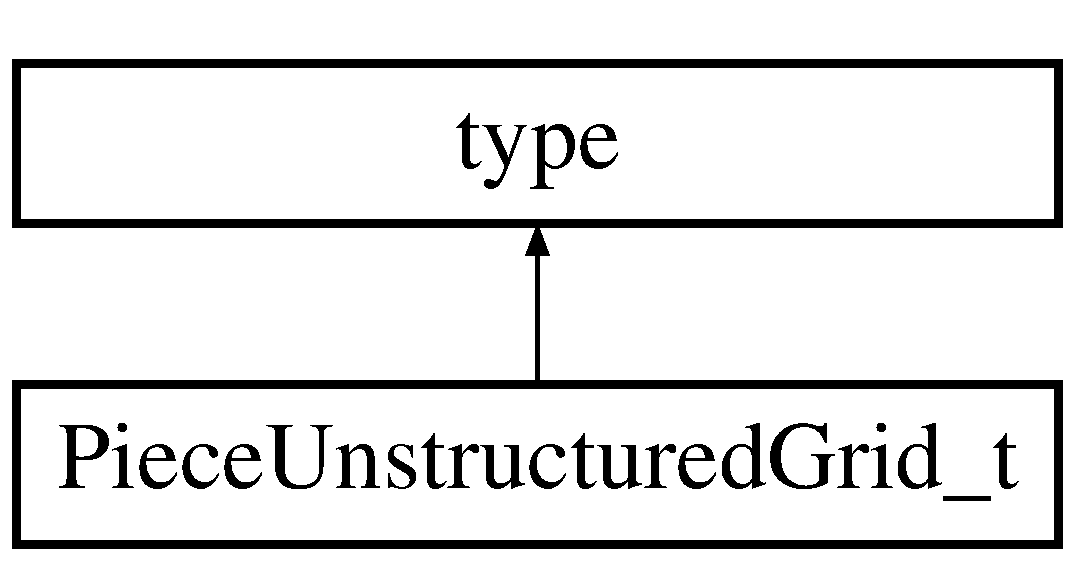
\includegraphics[height=2.000000cm]{classPieceUnstructuredGrid__t}
\end{center}
\end{figure}
\subsection*{Public Types}
\begin{DoxyCompactItemize}
\item 
typedef \+::\hyperlink{classPointData}{Point\+Data} \hyperlink{classPieceUnstructuredGrid__t_a5d79d8ea03ca53f80f24e62c2175ec02}{Point\+Data\+\_\+type}
\item 
typedef \+::xsd\+::cxx\+::tree\+::traits$<$ \hyperlink{classPieceUnstructuredGrid__t_a5d79d8ea03ca53f80f24e62c2175ec02}{Point\+Data\+\_\+type}, char $>$ \hyperlink{classPieceUnstructuredGrid__t_aee3c7ac7c46c4ebc9f248d31c458d300}{Point\+Data\+\_\+traits}
\item 
typedef \+::\hyperlink{classCellData}{Cell\+Data} \hyperlink{classPieceUnstructuredGrid__t_a4232a7b88477ee6f692a4e5fab6a65d1}{Cell\+Data\+\_\+type}
\item 
typedef \+::xsd\+::cxx\+::tree\+::traits$<$ \hyperlink{classPieceUnstructuredGrid__t_a4232a7b88477ee6f692a4e5fab6a65d1}{Cell\+Data\+\_\+type}, char $>$ \hyperlink{classPieceUnstructuredGrid__t_a0e04d369c16993da7e5e2a7152c2e518}{Cell\+Data\+\_\+traits}
\item 
typedef \+::\hyperlink{classPoints}{Points} \hyperlink{classPieceUnstructuredGrid__t_a7747b159a3d1eee8d02a0eefaa235711}{Points\+\_\+type}
\item 
typedef \+::xsd\+::cxx\+::tree\+::traits$<$ \hyperlink{classPieceUnstructuredGrid__t_a7747b159a3d1eee8d02a0eefaa235711}{Points\+\_\+type}, char $>$ \hyperlink{classPieceUnstructuredGrid__t_abdfd9c9f9eb5f43bd4cfcb2fad6d9f63}{Points\+\_\+traits}
\item 
typedef \+::\hyperlink{classCells}{Cells} \hyperlink{classPieceUnstructuredGrid__t_aca1ec38eff08bde0cd115c54dbb7a20f}{Cells\+\_\+type}
\item 
typedef \+::xsd\+::cxx\+::tree\+::traits$<$ \hyperlink{classPieceUnstructuredGrid__t_aca1ec38eff08bde0cd115c54dbb7a20f}{Cells\+\_\+type}, char $>$ \hyperlink{classPieceUnstructuredGrid__t_a33252b6f55b5ae830ceecdf9be42cce1}{Cells\+\_\+traits}
\item 
typedef \+::\hyperlink{namespacexml__schema_aaaea7c8ce4dfbe26cc52c91c29c97b7c}{xml\+\_\+schema\+::integer} \hyperlink{classPieceUnstructuredGrid__t_a8df1cd0d138d990e166d325ceed9a660}{Number\+Of\+Points\+\_\+type}
\item 
typedef \+::xsd\+::cxx\+::tree\+::traits$<$ \hyperlink{classPieceUnstructuredGrid__t_a8df1cd0d138d990e166d325ceed9a660}{Number\+Of\+Points\+\_\+type}, char $>$ \hyperlink{classPieceUnstructuredGrid__t_acdfbb1dc264a5a48bcc6d4aa815db003}{Number\+Of\+Points\+\_\+traits}
\item 
typedef \+::\hyperlink{namespacexml__schema_aaaea7c8ce4dfbe26cc52c91c29c97b7c}{xml\+\_\+schema\+::integer} \hyperlink{classPieceUnstructuredGrid__t_aeae5546900c50a4abe9b3aea485e97d0}{Number\+Of\+Cells\+\_\+type}
\item 
typedef \+::xsd\+::cxx\+::tree\+::traits$<$ \hyperlink{classPieceUnstructuredGrid__t_aeae5546900c50a4abe9b3aea485e97d0}{Number\+Of\+Cells\+\_\+type}, char $>$ \hyperlink{classPieceUnstructuredGrid__t_a7c7607d306bde9e187b9cb3f570d6155}{Number\+Of\+Cells\+\_\+traits}
\end{DoxyCompactItemize}
\subsection*{Public Member Functions}
\begin{DoxyCompactItemize}
\item 
const \hyperlink{classPieceUnstructuredGrid__t_a5d79d8ea03ca53f80f24e62c2175ec02}{Point\+Data\+\_\+type} \& \hyperlink{classPieceUnstructuredGrid__t_a4825627cfe05949b680c81826e9d4ea5}{Point\+Data} () const 
\item 
\hyperlink{classPieceUnstructuredGrid__t_a5d79d8ea03ca53f80f24e62c2175ec02}{Point\+Data\+\_\+type} \& \hyperlink{classPieceUnstructuredGrid__t_af3a9955626dac2aad17bf879a77d2c0d}{Point\+Data} ()
\item 
void \hyperlink{classPieceUnstructuredGrid__t_aee7745ad1ce39af5fc048e50acb76424}{Point\+Data} (const \hyperlink{classPieceUnstructuredGrid__t_a5d79d8ea03ca53f80f24e62c2175ec02}{Point\+Data\+\_\+type} \&x)
\item 
void \hyperlink{classPieceUnstructuredGrid__t_afb1080839846979d1870125471277dc2}{Point\+Data} (\+::std\+::unique\+\_\+ptr$<$ \hyperlink{classPieceUnstructuredGrid__t_a5d79d8ea03ca53f80f24e62c2175ec02}{Point\+Data\+\_\+type} $>$ p)
\item 
const \hyperlink{classPieceUnstructuredGrid__t_a4232a7b88477ee6f692a4e5fab6a65d1}{Cell\+Data\+\_\+type} \& \hyperlink{classPieceUnstructuredGrid__t_a7c7be2b175fa0ec2fc403bb4740865c1}{Cell\+Data} () const 
\item 
\hyperlink{classPieceUnstructuredGrid__t_a4232a7b88477ee6f692a4e5fab6a65d1}{Cell\+Data\+\_\+type} \& \hyperlink{classPieceUnstructuredGrid__t_a679db045d830876cce6fe04767e7c611}{Cell\+Data} ()
\item 
void \hyperlink{classPieceUnstructuredGrid__t_a6fd0984f28544ef312e860cac18e7144}{Cell\+Data} (const \hyperlink{classPieceUnstructuredGrid__t_a4232a7b88477ee6f692a4e5fab6a65d1}{Cell\+Data\+\_\+type} \&x)
\item 
void \hyperlink{classPieceUnstructuredGrid__t_acd0b16101f17e41b9af39f474c2d4d84}{Cell\+Data} (\+::std\+::unique\+\_\+ptr$<$ \hyperlink{classPieceUnstructuredGrid__t_a4232a7b88477ee6f692a4e5fab6a65d1}{Cell\+Data\+\_\+type} $>$ p)
\item 
const \hyperlink{classPieceUnstructuredGrid__t_a7747b159a3d1eee8d02a0eefaa235711}{Points\+\_\+type} \& \hyperlink{classPieceUnstructuredGrid__t_a53dfd670cb335d13003dc229343a0fa1}{Points} () const 
\item 
\hyperlink{classPieceUnstructuredGrid__t_a7747b159a3d1eee8d02a0eefaa235711}{Points\+\_\+type} \& \hyperlink{classPieceUnstructuredGrid__t_aa8e21b391979e8e2e22361e3b29e0276}{Points} ()
\item 
void \hyperlink{classPieceUnstructuredGrid__t_ab653af7be8fbe0d3458bf8cd5cdf3668}{Points} (const \hyperlink{classPieceUnstructuredGrid__t_a7747b159a3d1eee8d02a0eefaa235711}{Points\+\_\+type} \&x)
\item 
void \hyperlink{classPieceUnstructuredGrid__t_afec7f4ca6973137113fbc0932bee8642}{Points} (\+::std\+::unique\+\_\+ptr$<$ \hyperlink{classPieceUnstructuredGrid__t_a7747b159a3d1eee8d02a0eefaa235711}{Points\+\_\+type} $>$ p)
\item 
const \hyperlink{classPieceUnstructuredGrid__t_aca1ec38eff08bde0cd115c54dbb7a20f}{Cells\+\_\+type} \& \hyperlink{classPieceUnstructuredGrid__t_a398de7c2f319c1785810e18f6b43831e}{Cells} () const 
\item 
\hyperlink{classPieceUnstructuredGrid__t_aca1ec38eff08bde0cd115c54dbb7a20f}{Cells\+\_\+type} \& \hyperlink{classPieceUnstructuredGrid__t_a49e65eacff6577cd353fa15a09febf86}{Cells} ()
\item 
void \hyperlink{classPieceUnstructuredGrid__t_a366f0cff854ef350eb1be9da22df6d14}{Cells} (const \hyperlink{classPieceUnstructuredGrid__t_aca1ec38eff08bde0cd115c54dbb7a20f}{Cells\+\_\+type} \&x)
\item 
void \hyperlink{classPieceUnstructuredGrid__t_af45bb840ff71549e6728d774d1e36048}{Cells} (\+::std\+::unique\+\_\+ptr$<$ \hyperlink{classPieceUnstructuredGrid__t_aca1ec38eff08bde0cd115c54dbb7a20f}{Cells\+\_\+type} $>$ p)
\item 
const \hyperlink{classPieceUnstructuredGrid__t_a8df1cd0d138d990e166d325ceed9a660}{Number\+Of\+Points\+\_\+type} \& \hyperlink{classPieceUnstructuredGrid__t_a6fe4a92f59d9a837e046bf3d51e79b33}{Number\+Of\+Points} () const 
\item 
\hyperlink{classPieceUnstructuredGrid__t_a8df1cd0d138d990e166d325ceed9a660}{Number\+Of\+Points\+\_\+type} \& \hyperlink{classPieceUnstructuredGrid__t_adadae535c3c291dc01dd0be3315d9dbc}{Number\+Of\+Points} ()
\item 
void \hyperlink{classPieceUnstructuredGrid__t_a3e4e5defa42f9ecebb2016ca1d207700}{Number\+Of\+Points} (const \hyperlink{classPieceUnstructuredGrid__t_a8df1cd0d138d990e166d325ceed9a660}{Number\+Of\+Points\+\_\+type} \&x)
\item 
const \hyperlink{classPieceUnstructuredGrid__t_aeae5546900c50a4abe9b3aea485e97d0}{Number\+Of\+Cells\+\_\+type} \& \hyperlink{classPieceUnstructuredGrid__t_a6e395db39208cc81f9d7093c50d5d334}{Number\+Of\+Cells} () const 
\item 
\hyperlink{classPieceUnstructuredGrid__t_aeae5546900c50a4abe9b3aea485e97d0}{Number\+Of\+Cells\+\_\+type} \& \hyperlink{classPieceUnstructuredGrid__t_abe5f21a859d968d4b23a9b7ad790a7b3}{Number\+Of\+Cells} ()
\item 
void \hyperlink{classPieceUnstructuredGrid__t_a25296cecd9f9c30f8c75ed8b750c1ad7}{Number\+Of\+Cells} (const \hyperlink{classPieceUnstructuredGrid__t_aeae5546900c50a4abe9b3aea485e97d0}{Number\+Of\+Cells\+\_\+type} \&x)
\item 
\hyperlink{classPieceUnstructuredGrid__t_a9d30b76eb9efa7565011da966d5c0df7}{Piece\+Unstructured\+Grid\+\_\+t} (const \hyperlink{classPieceUnstructuredGrid__t_a5d79d8ea03ca53f80f24e62c2175ec02}{Point\+Data\+\_\+type} \&, const \hyperlink{classPieceUnstructuredGrid__t_a4232a7b88477ee6f692a4e5fab6a65d1}{Cell\+Data\+\_\+type} \&, const \hyperlink{classPieceUnstructuredGrid__t_a7747b159a3d1eee8d02a0eefaa235711}{Points\+\_\+type} \&, const \hyperlink{classPieceUnstructuredGrid__t_aca1ec38eff08bde0cd115c54dbb7a20f}{Cells\+\_\+type} \&, const \hyperlink{classPieceUnstructuredGrid__t_a8df1cd0d138d990e166d325ceed9a660}{Number\+Of\+Points\+\_\+type} \&, const \hyperlink{classPieceUnstructuredGrid__t_aeae5546900c50a4abe9b3aea485e97d0}{Number\+Of\+Cells\+\_\+type} \&)
\item 
\hyperlink{classPieceUnstructuredGrid__t_a76daa5e79a50b8d86dd39733313711e4}{Piece\+Unstructured\+Grid\+\_\+t} (\+::std\+::unique\+\_\+ptr$<$ \hyperlink{classPieceUnstructuredGrid__t_a5d79d8ea03ca53f80f24e62c2175ec02}{Point\+Data\+\_\+type} $>$,\+::std\+::unique\+\_\+ptr$<$ \hyperlink{classPieceUnstructuredGrid__t_a4232a7b88477ee6f692a4e5fab6a65d1}{Cell\+Data\+\_\+type} $>$,\+::std\+::unique\+\_\+ptr$<$ \hyperlink{classPieceUnstructuredGrid__t_a7747b159a3d1eee8d02a0eefaa235711}{Points\+\_\+type} $>$,\+::std\+::unique\+\_\+ptr$<$ \hyperlink{classPieceUnstructuredGrid__t_aca1ec38eff08bde0cd115c54dbb7a20f}{Cells\+\_\+type} $>$, const \hyperlink{classPieceUnstructuredGrid__t_a8df1cd0d138d990e166d325ceed9a660}{Number\+Of\+Points\+\_\+type} \&, const \hyperlink{classPieceUnstructuredGrid__t_aeae5546900c50a4abe9b3aea485e97d0}{Number\+Of\+Cells\+\_\+type} \&)
\item 
\hyperlink{classPieceUnstructuredGrid__t_a56c6d065b161aa4f28789044d082c622}{Piece\+Unstructured\+Grid\+\_\+t} (const \+::xercesc\+::\+D\+O\+M\+Element \&e,\+::\hyperlink{namespacexml__schema_a0612287d030cb2732d31a45b258fdc87}{xml\+\_\+schema\+::flags} f=0,\+::\hyperlink{namespacexml__schema_ada9aa30dc722e93ee2ed7243085402a5}{xml\+\_\+schema\+::container} $\ast$c=0)
\item 
\hyperlink{classPieceUnstructuredGrid__t_a6a1c61bdda2b5458715e902eae2420f9}{Piece\+Unstructured\+Grid\+\_\+t} (const \hyperlink{classPieceUnstructuredGrid__t}{Piece\+Unstructured\+Grid\+\_\+t} \&x,\+::\hyperlink{namespacexml__schema_a0612287d030cb2732d31a45b258fdc87}{xml\+\_\+schema\+::flags} f=0,\+::\hyperlink{namespacexml__schema_ada9aa30dc722e93ee2ed7243085402a5}{xml\+\_\+schema\+::container} $\ast$c=0)
\item 
virtual \hyperlink{classPieceUnstructuredGrid__t}{Piece\+Unstructured\+Grid\+\_\+t} $\ast$ \hyperlink{classPieceUnstructuredGrid__t_a48f6dcab2714e3f907993e1c99bcc8b2}{\+\_\+clone} (\+::\hyperlink{namespacexml__schema_a0612287d030cb2732d31a45b258fdc87}{xml\+\_\+schema\+::flags} f=0,\+::\hyperlink{namespacexml__schema_ada9aa30dc722e93ee2ed7243085402a5}{xml\+\_\+schema\+::container} $\ast$c=0) const 
\item 
\hyperlink{classPieceUnstructuredGrid__t}{Piece\+Unstructured\+Grid\+\_\+t} \& \hyperlink{classPieceUnstructuredGrid__t_ac314efbccef897349a02419c720a2d63}{operator=} (const \hyperlink{classPieceUnstructuredGrid__t}{Piece\+Unstructured\+Grid\+\_\+t} \&x)
\item 
virtual \hyperlink{classPieceUnstructuredGrid__t_a9d1eb720775ac4e3b7778f898decc264}{$\sim$\+Piece\+Unstructured\+Grid\+\_\+t} ()
\end{DoxyCompactItemize}
\subsection*{Protected Member Functions}
\begin{DoxyCompactItemize}
\item 
void \hyperlink{classPieceUnstructuredGrid__t_af30015c07de07a0ffb1f92eea8a48ebe}{parse} (\+::xsd\+::cxx\+::xml\+::dom\+::parser$<$ char $>$ \&,\+::\hyperlink{namespacexml__schema_a0612287d030cb2732d31a45b258fdc87}{xml\+\_\+schema\+::flags})
\end{DoxyCompactItemize}
\subsection*{Protected Attributes}
\begin{DoxyCompactItemize}
\item 
\+::xsd\+::cxx\+::tree\+::one$<$ \hyperlink{classPieceUnstructuredGrid__t_a5d79d8ea03ca53f80f24e62c2175ec02}{Point\+Data\+\_\+type} $>$ \hyperlink{classPieceUnstructuredGrid__t_a0c0f8305eeb054bb13a2ddcb702a40b9}{Point\+Data\+\_\+}
\item 
\+::xsd\+::cxx\+::tree\+::one$<$ \hyperlink{classPieceUnstructuredGrid__t_a4232a7b88477ee6f692a4e5fab6a65d1}{Cell\+Data\+\_\+type} $>$ \hyperlink{classPieceUnstructuredGrid__t_a4bc29dafe4e199e9584daa18f334fc27}{Cell\+Data\+\_\+}
\item 
\+::xsd\+::cxx\+::tree\+::one$<$ \hyperlink{classPieceUnstructuredGrid__t_a7747b159a3d1eee8d02a0eefaa235711}{Points\+\_\+type} $>$ \hyperlink{classPieceUnstructuredGrid__t_a661b6b8c1f38305c84b2864f496c37d8}{Points\+\_\+}
\item 
\+::xsd\+::cxx\+::tree\+::one$<$ \hyperlink{classPieceUnstructuredGrid__t_aca1ec38eff08bde0cd115c54dbb7a20f}{Cells\+\_\+type} $>$ \hyperlink{classPieceUnstructuredGrid__t_a8f3ced6893abfdf02faa2627d8f8c00c}{Cells\+\_\+}
\item 
\+::xsd\+::cxx\+::tree\+::one$<$ \hyperlink{classPieceUnstructuredGrid__t_a8df1cd0d138d990e166d325ceed9a660}{Number\+Of\+Points\+\_\+type} $>$ \hyperlink{classPieceUnstructuredGrid__t_ac16a2c2521aa4fd072a36b845cba38ef}{Number\+Of\+Points\+\_\+}
\item 
\+::xsd\+::cxx\+::tree\+::one$<$ \hyperlink{classPieceUnstructuredGrid__t_aeae5546900c50a4abe9b3aea485e97d0}{Number\+Of\+Cells\+\_\+type} $>$ \hyperlink{classPieceUnstructuredGrid__t_a3d55c06e74e3753fccc74f80a0886c32}{Number\+Of\+Cells\+\_\+}
\end{DoxyCompactItemize}


\subsection{Member Typedef Documentation}
\index{Piece\+Unstructured\+Grid\+\_\+t@{Piece\+Unstructured\+Grid\+\_\+t}!Cell\+Data\+\_\+traits@{Cell\+Data\+\_\+traits}}
\index{Cell\+Data\+\_\+traits@{Cell\+Data\+\_\+traits}!Piece\+Unstructured\+Grid\+\_\+t@{Piece\+Unstructured\+Grid\+\_\+t}}
\subsubsection[{\texorpdfstring{Cell\+Data\+\_\+traits}{CellData_traits}}]{\setlength{\rightskip}{0pt plus 5cm}typedef \+::xsd\+::cxx\+::tree\+::traits$<$ {\bf Cell\+Data\+\_\+type}, char $>$ {\bf Piece\+Unstructured\+Grid\+\_\+t\+::\+Cell\+Data\+\_\+traits}}\hypertarget{classPieceUnstructuredGrid__t_a0e04d369c16993da7e5e2a7152c2e518}{}\label{classPieceUnstructuredGrid__t_a0e04d369c16993da7e5e2a7152c2e518}
\index{Piece\+Unstructured\+Grid\+\_\+t@{Piece\+Unstructured\+Grid\+\_\+t}!Cell\+Data\+\_\+type@{Cell\+Data\+\_\+type}}
\index{Cell\+Data\+\_\+type@{Cell\+Data\+\_\+type}!Piece\+Unstructured\+Grid\+\_\+t@{Piece\+Unstructured\+Grid\+\_\+t}}
\subsubsection[{\texorpdfstring{Cell\+Data\+\_\+type}{CellData_type}}]{\setlength{\rightskip}{0pt plus 5cm}typedef \+::{\bf Cell\+Data} {\bf Piece\+Unstructured\+Grid\+\_\+t\+::\+Cell\+Data\+\_\+type}}\hypertarget{classPieceUnstructuredGrid__t_a4232a7b88477ee6f692a4e5fab6a65d1}{}\label{classPieceUnstructuredGrid__t_a4232a7b88477ee6f692a4e5fab6a65d1}
\index{Piece\+Unstructured\+Grid\+\_\+t@{Piece\+Unstructured\+Grid\+\_\+t}!Cells\+\_\+traits@{Cells\+\_\+traits}}
\index{Cells\+\_\+traits@{Cells\+\_\+traits}!Piece\+Unstructured\+Grid\+\_\+t@{Piece\+Unstructured\+Grid\+\_\+t}}
\subsubsection[{\texorpdfstring{Cells\+\_\+traits}{Cells_traits}}]{\setlength{\rightskip}{0pt plus 5cm}typedef \+::xsd\+::cxx\+::tree\+::traits$<$ {\bf Cells\+\_\+type}, char $>$ {\bf Piece\+Unstructured\+Grid\+\_\+t\+::\+Cells\+\_\+traits}}\hypertarget{classPieceUnstructuredGrid__t_a33252b6f55b5ae830ceecdf9be42cce1}{}\label{classPieceUnstructuredGrid__t_a33252b6f55b5ae830ceecdf9be42cce1}
\index{Piece\+Unstructured\+Grid\+\_\+t@{Piece\+Unstructured\+Grid\+\_\+t}!Cells\+\_\+type@{Cells\+\_\+type}}
\index{Cells\+\_\+type@{Cells\+\_\+type}!Piece\+Unstructured\+Grid\+\_\+t@{Piece\+Unstructured\+Grid\+\_\+t}}
\subsubsection[{\texorpdfstring{Cells\+\_\+type}{Cells_type}}]{\setlength{\rightskip}{0pt plus 5cm}typedef \+::{\bf Cells} {\bf Piece\+Unstructured\+Grid\+\_\+t\+::\+Cells\+\_\+type}}\hypertarget{classPieceUnstructuredGrid__t_aca1ec38eff08bde0cd115c54dbb7a20f}{}\label{classPieceUnstructuredGrid__t_aca1ec38eff08bde0cd115c54dbb7a20f}
\index{Piece\+Unstructured\+Grid\+\_\+t@{Piece\+Unstructured\+Grid\+\_\+t}!Number\+Of\+Cells\+\_\+traits@{Number\+Of\+Cells\+\_\+traits}}
\index{Number\+Of\+Cells\+\_\+traits@{Number\+Of\+Cells\+\_\+traits}!Piece\+Unstructured\+Grid\+\_\+t@{Piece\+Unstructured\+Grid\+\_\+t}}
\subsubsection[{\texorpdfstring{Number\+Of\+Cells\+\_\+traits}{NumberOfCells_traits}}]{\setlength{\rightskip}{0pt plus 5cm}typedef \+::xsd\+::cxx\+::tree\+::traits$<$ {\bf Number\+Of\+Cells\+\_\+type}, char $>$ {\bf Piece\+Unstructured\+Grid\+\_\+t\+::\+Number\+Of\+Cells\+\_\+traits}}\hypertarget{classPieceUnstructuredGrid__t_a7c7607d306bde9e187b9cb3f570d6155}{}\label{classPieceUnstructuredGrid__t_a7c7607d306bde9e187b9cb3f570d6155}
\index{Piece\+Unstructured\+Grid\+\_\+t@{Piece\+Unstructured\+Grid\+\_\+t}!Number\+Of\+Cells\+\_\+type@{Number\+Of\+Cells\+\_\+type}}
\index{Number\+Of\+Cells\+\_\+type@{Number\+Of\+Cells\+\_\+type}!Piece\+Unstructured\+Grid\+\_\+t@{Piece\+Unstructured\+Grid\+\_\+t}}
\subsubsection[{\texorpdfstring{Number\+Of\+Cells\+\_\+type}{NumberOfCells_type}}]{\setlength{\rightskip}{0pt plus 5cm}typedef \+::{\bf xml\+\_\+schema\+::integer} {\bf Piece\+Unstructured\+Grid\+\_\+t\+::\+Number\+Of\+Cells\+\_\+type}}\hypertarget{classPieceUnstructuredGrid__t_aeae5546900c50a4abe9b3aea485e97d0}{}\label{classPieceUnstructuredGrid__t_aeae5546900c50a4abe9b3aea485e97d0}
\index{Piece\+Unstructured\+Grid\+\_\+t@{Piece\+Unstructured\+Grid\+\_\+t}!Number\+Of\+Points\+\_\+traits@{Number\+Of\+Points\+\_\+traits}}
\index{Number\+Of\+Points\+\_\+traits@{Number\+Of\+Points\+\_\+traits}!Piece\+Unstructured\+Grid\+\_\+t@{Piece\+Unstructured\+Grid\+\_\+t}}
\subsubsection[{\texorpdfstring{Number\+Of\+Points\+\_\+traits}{NumberOfPoints_traits}}]{\setlength{\rightskip}{0pt plus 5cm}typedef \+::xsd\+::cxx\+::tree\+::traits$<$ {\bf Number\+Of\+Points\+\_\+type}, char $>$ {\bf Piece\+Unstructured\+Grid\+\_\+t\+::\+Number\+Of\+Points\+\_\+traits}}\hypertarget{classPieceUnstructuredGrid__t_acdfbb1dc264a5a48bcc6d4aa815db003}{}\label{classPieceUnstructuredGrid__t_acdfbb1dc264a5a48bcc6d4aa815db003}
\index{Piece\+Unstructured\+Grid\+\_\+t@{Piece\+Unstructured\+Grid\+\_\+t}!Number\+Of\+Points\+\_\+type@{Number\+Of\+Points\+\_\+type}}
\index{Number\+Of\+Points\+\_\+type@{Number\+Of\+Points\+\_\+type}!Piece\+Unstructured\+Grid\+\_\+t@{Piece\+Unstructured\+Grid\+\_\+t}}
\subsubsection[{\texorpdfstring{Number\+Of\+Points\+\_\+type}{NumberOfPoints_type}}]{\setlength{\rightskip}{0pt plus 5cm}typedef \+::{\bf xml\+\_\+schema\+::integer} {\bf Piece\+Unstructured\+Grid\+\_\+t\+::\+Number\+Of\+Points\+\_\+type}}\hypertarget{classPieceUnstructuredGrid__t_a8df1cd0d138d990e166d325ceed9a660}{}\label{classPieceUnstructuredGrid__t_a8df1cd0d138d990e166d325ceed9a660}
\index{Piece\+Unstructured\+Grid\+\_\+t@{Piece\+Unstructured\+Grid\+\_\+t}!Point\+Data\+\_\+traits@{Point\+Data\+\_\+traits}}
\index{Point\+Data\+\_\+traits@{Point\+Data\+\_\+traits}!Piece\+Unstructured\+Grid\+\_\+t@{Piece\+Unstructured\+Grid\+\_\+t}}
\subsubsection[{\texorpdfstring{Point\+Data\+\_\+traits}{PointData_traits}}]{\setlength{\rightskip}{0pt plus 5cm}typedef \+::xsd\+::cxx\+::tree\+::traits$<$ {\bf Point\+Data\+\_\+type}, char $>$ {\bf Piece\+Unstructured\+Grid\+\_\+t\+::\+Point\+Data\+\_\+traits}}\hypertarget{classPieceUnstructuredGrid__t_aee3c7ac7c46c4ebc9f248d31c458d300}{}\label{classPieceUnstructuredGrid__t_aee3c7ac7c46c4ebc9f248d31c458d300}
\index{Piece\+Unstructured\+Grid\+\_\+t@{Piece\+Unstructured\+Grid\+\_\+t}!Point\+Data\+\_\+type@{Point\+Data\+\_\+type}}
\index{Point\+Data\+\_\+type@{Point\+Data\+\_\+type}!Piece\+Unstructured\+Grid\+\_\+t@{Piece\+Unstructured\+Grid\+\_\+t}}
\subsubsection[{\texorpdfstring{Point\+Data\+\_\+type}{PointData_type}}]{\setlength{\rightskip}{0pt plus 5cm}typedef \+::{\bf Point\+Data} {\bf Piece\+Unstructured\+Grid\+\_\+t\+::\+Point\+Data\+\_\+type}}\hypertarget{classPieceUnstructuredGrid__t_a5d79d8ea03ca53f80f24e62c2175ec02}{}\label{classPieceUnstructuredGrid__t_a5d79d8ea03ca53f80f24e62c2175ec02}
\index{Piece\+Unstructured\+Grid\+\_\+t@{Piece\+Unstructured\+Grid\+\_\+t}!Points\+\_\+traits@{Points\+\_\+traits}}
\index{Points\+\_\+traits@{Points\+\_\+traits}!Piece\+Unstructured\+Grid\+\_\+t@{Piece\+Unstructured\+Grid\+\_\+t}}
\subsubsection[{\texorpdfstring{Points\+\_\+traits}{Points_traits}}]{\setlength{\rightskip}{0pt plus 5cm}typedef \+::xsd\+::cxx\+::tree\+::traits$<$ {\bf Points\+\_\+type}, char $>$ {\bf Piece\+Unstructured\+Grid\+\_\+t\+::\+Points\+\_\+traits}}\hypertarget{classPieceUnstructuredGrid__t_abdfd9c9f9eb5f43bd4cfcb2fad6d9f63}{}\label{classPieceUnstructuredGrid__t_abdfd9c9f9eb5f43bd4cfcb2fad6d9f63}
\index{Piece\+Unstructured\+Grid\+\_\+t@{Piece\+Unstructured\+Grid\+\_\+t}!Points\+\_\+type@{Points\+\_\+type}}
\index{Points\+\_\+type@{Points\+\_\+type}!Piece\+Unstructured\+Grid\+\_\+t@{Piece\+Unstructured\+Grid\+\_\+t}}
\subsubsection[{\texorpdfstring{Points\+\_\+type}{Points_type}}]{\setlength{\rightskip}{0pt plus 5cm}typedef \+::{\bf Points} {\bf Piece\+Unstructured\+Grid\+\_\+t\+::\+Points\+\_\+type}}\hypertarget{classPieceUnstructuredGrid__t_a7747b159a3d1eee8d02a0eefaa235711}{}\label{classPieceUnstructuredGrid__t_a7747b159a3d1eee8d02a0eefaa235711}


\subsection{Constructor \& Destructor Documentation}
\index{Piece\+Unstructured\+Grid\+\_\+t@{Piece\+Unstructured\+Grid\+\_\+t}!Piece\+Unstructured\+Grid\+\_\+t@{Piece\+Unstructured\+Grid\+\_\+t}}
\index{Piece\+Unstructured\+Grid\+\_\+t@{Piece\+Unstructured\+Grid\+\_\+t}!Piece\+Unstructured\+Grid\+\_\+t@{Piece\+Unstructured\+Grid\+\_\+t}}
\subsubsection[{\texorpdfstring{Piece\+Unstructured\+Grid\+\_\+t(const Point\+Data\+\_\+type \&, const Cell\+Data\+\_\+type \&, const Points\+\_\+type \&, const Cells\+\_\+type \&, const Number\+Of\+Points\+\_\+type \&, const Number\+Of\+Cells\+\_\+type \&)}{PieceUnstructuredGrid_t(const PointData_type &, const CellData_type &, const Points_type &, const Cells_type &, const NumberOfPoints_type &, const NumberOfCells_type &)}}]{\setlength{\rightskip}{0pt plus 5cm}Piece\+Unstructured\+Grid\+\_\+t\+::\+Piece\+Unstructured\+Grid\+\_\+t (
\begin{DoxyParamCaption}
\item[{const {\bf Point\+Data\+\_\+type} \&}]{Point\+Data, }
\item[{const {\bf Cell\+Data\+\_\+type} \&}]{Cell\+Data, }
\item[{const {\bf Points\+\_\+type} \&}]{Points, }
\item[{const {\bf Cells\+\_\+type} \&}]{Cells, }
\item[{const {\bf Number\+Of\+Points\+\_\+type} \&}]{Number\+Of\+Points, }
\item[{const {\bf Number\+Of\+Cells\+\_\+type} \&}]{Number\+Of\+Cells}
\end{DoxyParamCaption}
)}\hypertarget{classPieceUnstructuredGrid__t_a9d30b76eb9efa7565011da966d5c0df7}{}\label{classPieceUnstructuredGrid__t_a9d30b76eb9efa7565011da966d5c0df7}
\index{Piece\+Unstructured\+Grid\+\_\+t@{Piece\+Unstructured\+Grid\+\_\+t}!Piece\+Unstructured\+Grid\+\_\+t@{Piece\+Unstructured\+Grid\+\_\+t}}
\index{Piece\+Unstructured\+Grid\+\_\+t@{Piece\+Unstructured\+Grid\+\_\+t}!Piece\+Unstructured\+Grid\+\_\+t@{Piece\+Unstructured\+Grid\+\_\+t}}
\subsubsection[{\texorpdfstring{Piece\+Unstructured\+Grid\+\_\+t(\+::std\+::unique\+\_\+ptr$<$ Point\+Data\+\_\+type $>$,\+::std\+::unique\+\_\+ptr$<$ Cell\+Data\+\_\+type $>$,\+::std\+::unique\+\_\+ptr$<$ Points\+\_\+type $>$,\+::std\+::unique\+\_\+ptr$<$ Cells\+\_\+type $>$, const Number\+Of\+Points\+\_\+type \&, const Number\+Of\+Cells\+\_\+type \&)}{PieceUnstructuredGrid_t(::std::unique_ptr< PointData_type >,::std::unique_ptr< CellData_type >,::std::unique_ptr< Points_type >,::std::unique_ptr< Cells_type >, const NumberOfPoints_type &, const NumberOfCells_type &)}}]{\setlength{\rightskip}{0pt plus 5cm}Piece\+Unstructured\+Grid\+\_\+t\+::\+Piece\+Unstructured\+Grid\+\_\+t (
\begin{DoxyParamCaption}
\item[{\+::std\+::unique\+\_\+ptr$<$ {\bf Point\+Data\+\_\+type} $>$}]{Point\+Data, }
\item[{\+::std\+::unique\+\_\+ptr$<$ {\bf Cell\+Data\+\_\+type} $>$}]{Cell\+Data, }
\item[{\+::std\+::unique\+\_\+ptr$<$ {\bf Points\+\_\+type} $>$}]{Points, }
\item[{\+::std\+::unique\+\_\+ptr$<$ {\bf Cells\+\_\+type} $>$}]{Cells, }
\item[{const {\bf Number\+Of\+Points\+\_\+type} \&}]{Number\+Of\+Points, }
\item[{const {\bf Number\+Of\+Cells\+\_\+type} \&}]{Number\+Of\+Cells}
\end{DoxyParamCaption}
)}\hypertarget{classPieceUnstructuredGrid__t_a76daa5e79a50b8d86dd39733313711e4}{}\label{classPieceUnstructuredGrid__t_a76daa5e79a50b8d86dd39733313711e4}
\index{Piece\+Unstructured\+Grid\+\_\+t@{Piece\+Unstructured\+Grid\+\_\+t}!Piece\+Unstructured\+Grid\+\_\+t@{Piece\+Unstructured\+Grid\+\_\+t}}
\index{Piece\+Unstructured\+Grid\+\_\+t@{Piece\+Unstructured\+Grid\+\_\+t}!Piece\+Unstructured\+Grid\+\_\+t@{Piece\+Unstructured\+Grid\+\_\+t}}
\subsubsection[{\texorpdfstring{Piece\+Unstructured\+Grid\+\_\+t(const \+::xercesc\+::\+D\+O\+M\+Element \&e,\+::xml\+\_\+schema\+::flags f=0,\+::xml\+\_\+schema\+::container $\ast$c=0)}{PieceUnstructuredGrid_t(const ::xercesc::DOMElement &e,::xml_schema::flags f=0,::xml_schema::container *c=0)}}]{\setlength{\rightskip}{0pt plus 5cm}Piece\+Unstructured\+Grid\+\_\+t\+::\+Piece\+Unstructured\+Grid\+\_\+t (
\begin{DoxyParamCaption}
\item[{const \+::xercesc\+::\+D\+O\+M\+Element \&}]{e, }
\item[{\+::{\bf xml\+\_\+schema\+::flags}}]{f = {\ttfamily 0}, }
\item[{\+::{\bf xml\+\_\+schema\+::container} $\ast$}]{c = {\ttfamily 0}}
\end{DoxyParamCaption}
)}\hypertarget{classPieceUnstructuredGrid__t_a56c6d065b161aa4f28789044d082c622}{}\label{classPieceUnstructuredGrid__t_a56c6d065b161aa4f28789044d082c622}
\index{Piece\+Unstructured\+Grid\+\_\+t@{Piece\+Unstructured\+Grid\+\_\+t}!Piece\+Unstructured\+Grid\+\_\+t@{Piece\+Unstructured\+Grid\+\_\+t}}
\index{Piece\+Unstructured\+Grid\+\_\+t@{Piece\+Unstructured\+Grid\+\_\+t}!Piece\+Unstructured\+Grid\+\_\+t@{Piece\+Unstructured\+Grid\+\_\+t}}
\subsubsection[{\texorpdfstring{Piece\+Unstructured\+Grid\+\_\+t(const Piece\+Unstructured\+Grid\+\_\+t \&x,\+::xml\+\_\+schema\+::flags f=0,\+::xml\+\_\+schema\+::container $\ast$c=0)}{PieceUnstructuredGrid_t(const PieceUnstructuredGrid_t &x,::xml_schema::flags f=0,::xml_schema::container *c=0)}}]{\setlength{\rightskip}{0pt plus 5cm}Piece\+Unstructured\+Grid\+\_\+t\+::\+Piece\+Unstructured\+Grid\+\_\+t (
\begin{DoxyParamCaption}
\item[{const {\bf Piece\+Unstructured\+Grid\+\_\+t} \&}]{x, }
\item[{\+::{\bf xml\+\_\+schema\+::flags}}]{f = {\ttfamily 0}, }
\item[{\+::{\bf xml\+\_\+schema\+::container} $\ast$}]{c = {\ttfamily 0}}
\end{DoxyParamCaption}
)}\hypertarget{classPieceUnstructuredGrid__t_a6a1c61bdda2b5458715e902eae2420f9}{}\label{classPieceUnstructuredGrid__t_a6a1c61bdda2b5458715e902eae2420f9}
\index{Piece\+Unstructured\+Grid\+\_\+t@{Piece\+Unstructured\+Grid\+\_\+t}!````~Piece\+Unstructured\+Grid\+\_\+t@{$\sim$\+Piece\+Unstructured\+Grid\+\_\+t}}
\index{````~Piece\+Unstructured\+Grid\+\_\+t@{$\sim$\+Piece\+Unstructured\+Grid\+\_\+t}!Piece\+Unstructured\+Grid\+\_\+t@{Piece\+Unstructured\+Grid\+\_\+t}}
\subsubsection[{\texorpdfstring{$\sim$\+Piece\+Unstructured\+Grid\+\_\+t()}{~PieceUnstructuredGrid_t()}}]{\setlength{\rightskip}{0pt plus 5cm}Piece\+Unstructured\+Grid\+\_\+t\+::$\sim$\+Piece\+Unstructured\+Grid\+\_\+t (
\begin{DoxyParamCaption}
{}
\end{DoxyParamCaption}
)\hspace{0.3cm}{\ttfamily [virtual]}}\hypertarget{classPieceUnstructuredGrid__t_a9d1eb720775ac4e3b7778f898decc264}{}\label{classPieceUnstructuredGrid__t_a9d1eb720775ac4e3b7778f898decc264}


\subsection{Member Function Documentation}
\index{Piece\+Unstructured\+Grid\+\_\+t@{Piece\+Unstructured\+Grid\+\_\+t}!\+\_\+clone@{\+\_\+clone}}
\index{\+\_\+clone@{\+\_\+clone}!Piece\+Unstructured\+Grid\+\_\+t@{Piece\+Unstructured\+Grid\+\_\+t}}
\subsubsection[{\texorpdfstring{\+\_\+clone(\+::xml\+\_\+schema\+::flags f=0,\+::xml\+\_\+schema\+::container $\ast$c=0) const }{_clone(::xml_schema::flags f=0,::xml_schema::container *c=0) const }}]{\setlength{\rightskip}{0pt plus 5cm}{\bf Piece\+Unstructured\+Grid\+\_\+t} $\ast$ Piece\+Unstructured\+Grid\+\_\+t\+::\+\_\+clone (
\begin{DoxyParamCaption}
\item[{\+::{\bf xml\+\_\+schema\+::flags}}]{f = {\ttfamily 0}, }
\item[{\+::{\bf xml\+\_\+schema\+::container} $\ast$}]{c = {\ttfamily 0}}
\end{DoxyParamCaption}
) const\hspace{0.3cm}{\ttfamily [virtual]}}\hypertarget{classPieceUnstructuredGrid__t_a48f6dcab2714e3f907993e1c99bcc8b2}{}\label{classPieceUnstructuredGrid__t_a48f6dcab2714e3f907993e1c99bcc8b2}
\index{Piece\+Unstructured\+Grid\+\_\+t@{Piece\+Unstructured\+Grid\+\_\+t}!Cell\+Data@{Cell\+Data}}
\index{Cell\+Data@{Cell\+Data}!Piece\+Unstructured\+Grid\+\_\+t@{Piece\+Unstructured\+Grid\+\_\+t}}
\subsubsection[{\texorpdfstring{Cell\+Data() const }{CellData() const }}]{\setlength{\rightskip}{0pt plus 5cm}const {\bf Piece\+Unstructured\+Grid\+\_\+t\+::\+Cell\+Data\+\_\+type} \& Piece\+Unstructured\+Grid\+\_\+t\+::\+Cell\+Data (
\begin{DoxyParamCaption}
{}
\end{DoxyParamCaption}
) const}\hypertarget{classPieceUnstructuredGrid__t_a7c7be2b175fa0ec2fc403bb4740865c1}{}\label{classPieceUnstructuredGrid__t_a7c7be2b175fa0ec2fc403bb4740865c1}
\index{Piece\+Unstructured\+Grid\+\_\+t@{Piece\+Unstructured\+Grid\+\_\+t}!Cell\+Data@{Cell\+Data}}
\index{Cell\+Data@{Cell\+Data}!Piece\+Unstructured\+Grid\+\_\+t@{Piece\+Unstructured\+Grid\+\_\+t}}
\subsubsection[{\texorpdfstring{Cell\+Data()}{CellData()}}]{\setlength{\rightskip}{0pt plus 5cm}{\bf Piece\+Unstructured\+Grid\+\_\+t\+::\+Cell\+Data\+\_\+type} \& Piece\+Unstructured\+Grid\+\_\+t\+::\+Cell\+Data (
\begin{DoxyParamCaption}
{}
\end{DoxyParamCaption}
)}\hypertarget{classPieceUnstructuredGrid__t_a679db045d830876cce6fe04767e7c611}{}\label{classPieceUnstructuredGrid__t_a679db045d830876cce6fe04767e7c611}
\index{Piece\+Unstructured\+Grid\+\_\+t@{Piece\+Unstructured\+Grid\+\_\+t}!Cell\+Data@{Cell\+Data}}
\index{Cell\+Data@{Cell\+Data}!Piece\+Unstructured\+Grid\+\_\+t@{Piece\+Unstructured\+Grid\+\_\+t}}
\subsubsection[{\texorpdfstring{Cell\+Data(const Cell\+Data\+\_\+type \&x)}{CellData(const CellData_type &x)}}]{\setlength{\rightskip}{0pt plus 5cm}void Piece\+Unstructured\+Grid\+\_\+t\+::\+Cell\+Data (
\begin{DoxyParamCaption}
\item[{const {\bf Cell\+Data\+\_\+type} \&}]{x}
\end{DoxyParamCaption}
)}\hypertarget{classPieceUnstructuredGrid__t_a6fd0984f28544ef312e860cac18e7144}{}\label{classPieceUnstructuredGrid__t_a6fd0984f28544ef312e860cac18e7144}
\index{Piece\+Unstructured\+Grid\+\_\+t@{Piece\+Unstructured\+Grid\+\_\+t}!Cell\+Data@{Cell\+Data}}
\index{Cell\+Data@{Cell\+Data}!Piece\+Unstructured\+Grid\+\_\+t@{Piece\+Unstructured\+Grid\+\_\+t}}
\subsubsection[{\texorpdfstring{Cell\+Data(\+::std\+::unique\+\_\+ptr$<$ Cell\+Data\+\_\+type $>$ p)}{CellData(::std::unique_ptr< CellData_type > p)}}]{\setlength{\rightskip}{0pt plus 5cm}void Piece\+Unstructured\+Grid\+\_\+t\+::\+Cell\+Data (
\begin{DoxyParamCaption}
\item[{\+::std\+::unique\+\_\+ptr$<$ {\bf Cell\+Data\+\_\+type} $>$}]{p}
\end{DoxyParamCaption}
)}\hypertarget{classPieceUnstructuredGrid__t_acd0b16101f17e41b9af39f474c2d4d84}{}\label{classPieceUnstructuredGrid__t_acd0b16101f17e41b9af39f474c2d4d84}
\index{Piece\+Unstructured\+Grid\+\_\+t@{Piece\+Unstructured\+Grid\+\_\+t}!Cells@{Cells}}
\index{Cells@{Cells}!Piece\+Unstructured\+Grid\+\_\+t@{Piece\+Unstructured\+Grid\+\_\+t}}
\subsubsection[{\texorpdfstring{Cells() const }{Cells() const }}]{\setlength{\rightskip}{0pt plus 5cm}const {\bf Piece\+Unstructured\+Grid\+\_\+t\+::\+Cells\+\_\+type} \& Piece\+Unstructured\+Grid\+\_\+t\+::\+Cells (
\begin{DoxyParamCaption}
{}
\end{DoxyParamCaption}
) const}\hypertarget{classPieceUnstructuredGrid__t_a398de7c2f319c1785810e18f6b43831e}{}\label{classPieceUnstructuredGrid__t_a398de7c2f319c1785810e18f6b43831e}
\index{Piece\+Unstructured\+Grid\+\_\+t@{Piece\+Unstructured\+Grid\+\_\+t}!Cells@{Cells}}
\index{Cells@{Cells}!Piece\+Unstructured\+Grid\+\_\+t@{Piece\+Unstructured\+Grid\+\_\+t}}
\subsubsection[{\texorpdfstring{Cells()}{Cells()}}]{\setlength{\rightskip}{0pt plus 5cm}{\bf Piece\+Unstructured\+Grid\+\_\+t\+::\+Cells\+\_\+type} \& Piece\+Unstructured\+Grid\+\_\+t\+::\+Cells (
\begin{DoxyParamCaption}
{}
\end{DoxyParamCaption}
)}\hypertarget{classPieceUnstructuredGrid__t_a49e65eacff6577cd353fa15a09febf86}{}\label{classPieceUnstructuredGrid__t_a49e65eacff6577cd353fa15a09febf86}
\index{Piece\+Unstructured\+Grid\+\_\+t@{Piece\+Unstructured\+Grid\+\_\+t}!Cells@{Cells}}
\index{Cells@{Cells}!Piece\+Unstructured\+Grid\+\_\+t@{Piece\+Unstructured\+Grid\+\_\+t}}
\subsubsection[{\texorpdfstring{Cells(const Cells\+\_\+type \&x)}{Cells(const Cells_type &x)}}]{\setlength{\rightskip}{0pt plus 5cm}void Piece\+Unstructured\+Grid\+\_\+t\+::\+Cells (
\begin{DoxyParamCaption}
\item[{const {\bf Cells\+\_\+type} \&}]{x}
\end{DoxyParamCaption}
)}\hypertarget{classPieceUnstructuredGrid__t_a366f0cff854ef350eb1be9da22df6d14}{}\label{classPieceUnstructuredGrid__t_a366f0cff854ef350eb1be9da22df6d14}
\index{Piece\+Unstructured\+Grid\+\_\+t@{Piece\+Unstructured\+Grid\+\_\+t}!Cells@{Cells}}
\index{Cells@{Cells}!Piece\+Unstructured\+Grid\+\_\+t@{Piece\+Unstructured\+Grid\+\_\+t}}
\subsubsection[{\texorpdfstring{Cells(\+::std\+::unique\+\_\+ptr$<$ Cells\+\_\+type $>$ p)}{Cells(::std::unique_ptr< Cells_type > p)}}]{\setlength{\rightskip}{0pt plus 5cm}void Piece\+Unstructured\+Grid\+\_\+t\+::\+Cells (
\begin{DoxyParamCaption}
\item[{\+::std\+::unique\+\_\+ptr$<$ {\bf Cells\+\_\+type} $>$}]{p}
\end{DoxyParamCaption}
)}\hypertarget{classPieceUnstructuredGrid__t_af45bb840ff71549e6728d774d1e36048}{}\label{classPieceUnstructuredGrid__t_af45bb840ff71549e6728d774d1e36048}
\index{Piece\+Unstructured\+Grid\+\_\+t@{Piece\+Unstructured\+Grid\+\_\+t}!Number\+Of\+Cells@{Number\+Of\+Cells}}
\index{Number\+Of\+Cells@{Number\+Of\+Cells}!Piece\+Unstructured\+Grid\+\_\+t@{Piece\+Unstructured\+Grid\+\_\+t}}
\subsubsection[{\texorpdfstring{Number\+Of\+Cells() const }{NumberOfCells() const }}]{\setlength{\rightskip}{0pt plus 5cm}const {\bf Piece\+Unstructured\+Grid\+\_\+t\+::\+Number\+Of\+Cells\+\_\+type} \& Piece\+Unstructured\+Grid\+\_\+t\+::\+Number\+Of\+Cells (
\begin{DoxyParamCaption}
{}
\end{DoxyParamCaption}
) const}\hypertarget{classPieceUnstructuredGrid__t_a6e395db39208cc81f9d7093c50d5d334}{}\label{classPieceUnstructuredGrid__t_a6e395db39208cc81f9d7093c50d5d334}
\index{Piece\+Unstructured\+Grid\+\_\+t@{Piece\+Unstructured\+Grid\+\_\+t}!Number\+Of\+Cells@{Number\+Of\+Cells}}
\index{Number\+Of\+Cells@{Number\+Of\+Cells}!Piece\+Unstructured\+Grid\+\_\+t@{Piece\+Unstructured\+Grid\+\_\+t}}
\subsubsection[{\texorpdfstring{Number\+Of\+Cells()}{NumberOfCells()}}]{\setlength{\rightskip}{0pt plus 5cm}{\bf Piece\+Unstructured\+Grid\+\_\+t\+::\+Number\+Of\+Cells\+\_\+type} \& Piece\+Unstructured\+Grid\+\_\+t\+::\+Number\+Of\+Cells (
\begin{DoxyParamCaption}
{}
\end{DoxyParamCaption}
)}\hypertarget{classPieceUnstructuredGrid__t_abe5f21a859d968d4b23a9b7ad790a7b3}{}\label{classPieceUnstructuredGrid__t_abe5f21a859d968d4b23a9b7ad790a7b3}
\index{Piece\+Unstructured\+Grid\+\_\+t@{Piece\+Unstructured\+Grid\+\_\+t}!Number\+Of\+Cells@{Number\+Of\+Cells}}
\index{Number\+Of\+Cells@{Number\+Of\+Cells}!Piece\+Unstructured\+Grid\+\_\+t@{Piece\+Unstructured\+Grid\+\_\+t}}
\subsubsection[{\texorpdfstring{Number\+Of\+Cells(const Number\+Of\+Cells\+\_\+type \&x)}{NumberOfCells(const NumberOfCells_type &x)}}]{\setlength{\rightskip}{0pt plus 5cm}void Piece\+Unstructured\+Grid\+\_\+t\+::\+Number\+Of\+Cells (
\begin{DoxyParamCaption}
\item[{const {\bf Number\+Of\+Cells\+\_\+type} \&}]{x}
\end{DoxyParamCaption}
)}\hypertarget{classPieceUnstructuredGrid__t_a25296cecd9f9c30f8c75ed8b750c1ad7}{}\label{classPieceUnstructuredGrid__t_a25296cecd9f9c30f8c75ed8b750c1ad7}
\index{Piece\+Unstructured\+Grid\+\_\+t@{Piece\+Unstructured\+Grid\+\_\+t}!Number\+Of\+Points@{Number\+Of\+Points}}
\index{Number\+Of\+Points@{Number\+Of\+Points}!Piece\+Unstructured\+Grid\+\_\+t@{Piece\+Unstructured\+Grid\+\_\+t}}
\subsubsection[{\texorpdfstring{Number\+Of\+Points() const }{NumberOfPoints() const }}]{\setlength{\rightskip}{0pt plus 5cm}const {\bf Piece\+Unstructured\+Grid\+\_\+t\+::\+Number\+Of\+Points\+\_\+type} \& Piece\+Unstructured\+Grid\+\_\+t\+::\+Number\+Of\+Points (
\begin{DoxyParamCaption}
{}
\end{DoxyParamCaption}
) const}\hypertarget{classPieceUnstructuredGrid__t_a6fe4a92f59d9a837e046bf3d51e79b33}{}\label{classPieceUnstructuredGrid__t_a6fe4a92f59d9a837e046bf3d51e79b33}
\index{Piece\+Unstructured\+Grid\+\_\+t@{Piece\+Unstructured\+Grid\+\_\+t}!Number\+Of\+Points@{Number\+Of\+Points}}
\index{Number\+Of\+Points@{Number\+Of\+Points}!Piece\+Unstructured\+Grid\+\_\+t@{Piece\+Unstructured\+Grid\+\_\+t}}
\subsubsection[{\texorpdfstring{Number\+Of\+Points()}{NumberOfPoints()}}]{\setlength{\rightskip}{0pt plus 5cm}{\bf Piece\+Unstructured\+Grid\+\_\+t\+::\+Number\+Of\+Points\+\_\+type} \& Piece\+Unstructured\+Grid\+\_\+t\+::\+Number\+Of\+Points (
\begin{DoxyParamCaption}
{}
\end{DoxyParamCaption}
)}\hypertarget{classPieceUnstructuredGrid__t_adadae535c3c291dc01dd0be3315d9dbc}{}\label{classPieceUnstructuredGrid__t_adadae535c3c291dc01dd0be3315d9dbc}
\index{Piece\+Unstructured\+Grid\+\_\+t@{Piece\+Unstructured\+Grid\+\_\+t}!Number\+Of\+Points@{Number\+Of\+Points}}
\index{Number\+Of\+Points@{Number\+Of\+Points}!Piece\+Unstructured\+Grid\+\_\+t@{Piece\+Unstructured\+Grid\+\_\+t}}
\subsubsection[{\texorpdfstring{Number\+Of\+Points(const Number\+Of\+Points\+\_\+type \&x)}{NumberOfPoints(const NumberOfPoints_type &x)}}]{\setlength{\rightskip}{0pt plus 5cm}void Piece\+Unstructured\+Grid\+\_\+t\+::\+Number\+Of\+Points (
\begin{DoxyParamCaption}
\item[{const {\bf Number\+Of\+Points\+\_\+type} \&}]{x}
\end{DoxyParamCaption}
)}\hypertarget{classPieceUnstructuredGrid__t_a3e4e5defa42f9ecebb2016ca1d207700}{}\label{classPieceUnstructuredGrid__t_a3e4e5defa42f9ecebb2016ca1d207700}
\index{Piece\+Unstructured\+Grid\+\_\+t@{Piece\+Unstructured\+Grid\+\_\+t}!operator=@{operator=}}
\index{operator=@{operator=}!Piece\+Unstructured\+Grid\+\_\+t@{Piece\+Unstructured\+Grid\+\_\+t}}
\subsubsection[{\texorpdfstring{operator=(const Piece\+Unstructured\+Grid\+\_\+t \&x)}{operator=(const PieceUnstructuredGrid_t &x)}}]{\setlength{\rightskip}{0pt plus 5cm}{\bf Piece\+Unstructured\+Grid\+\_\+t} \& Piece\+Unstructured\+Grid\+\_\+t\+::operator= (
\begin{DoxyParamCaption}
\item[{const {\bf Piece\+Unstructured\+Grid\+\_\+t} \&}]{x}
\end{DoxyParamCaption}
)}\hypertarget{classPieceUnstructuredGrid__t_ac314efbccef897349a02419c720a2d63}{}\label{classPieceUnstructuredGrid__t_ac314efbccef897349a02419c720a2d63}
\index{Piece\+Unstructured\+Grid\+\_\+t@{Piece\+Unstructured\+Grid\+\_\+t}!parse@{parse}}
\index{parse@{parse}!Piece\+Unstructured\+Grid\+\_\+t@{Piece\+Unstructured\+Grid\+\_\+t}}
\subsubsection[{\texorpdfstring{parse(\+::xsd\+::cxx\+::xml\+::dom\+::parser$<$ char $>$ \&,\+::xml\+\_\+schema\+::flags)}{parse(::xsd::cxx::xml::dom::parser< char > &,::xml_schema::flags)}}]{\setlength{\rightskip}{0pt plus 5cm}void Piece\+Unstructured\+Grid\+\_\+t\+::parse (
\begin{DoxyParamCaption}
\item[{\+::xsd\+::cxx\+::xml\+::dom\+::parser$<$ char $>$ \&}]{p, }
\item[{\+::{\bf xml\+\_\+schema\+::flags}}]{f}
\end{DoxyParamCaption}
)\hspace{0.3cm}{\ttfamily [protected]}}\hypertarget{classPieceUnstructuredGrid__t_af30015c07de07a0ffb1f92eea8a48ebe}{}\label{classPieceUnstructuredGrid__t_af30015c07de07a0ffb1f92eea8a48ebe}
\index{Piece\+Unstructured\+Grid\+\_\+t@{Piece\+Unstructured\+Grid\+\_\+t}!Point\+Data@{Point\+Data}}
\index{Point\+Data@{Point\+Data}!Piece\+Unstructured\+Grid\+\_\+t@{Piece\+Unstructured\+Grid\+\_\+t}}
\subsubsection[{\texorpdfstring{Point\+Data() const }{PointData() const }}]{\setlength{\rightskip}{0pt plus 5cm}const {\bf Piece\+Unstructured\+Grid\+\_\+t\+::\+Point\+Data\+\_\+type} \& Piece\+Unstructured\+Grid\+\_\+t\+::\+Point\+Data (
\begin{DoxyParamCaption}
{}
\end{DoxyParamCaption}
) const}\hypertarget{classPieceUnstructuredGrid__t_a4825627cfe05949b680c81826e9d4ea5}{}\label{classPieceUnstructuredGrid__t_a4825627cfe05949b680c81826e9d4ea5}
\index{Piece\+Unstructured\+Grid\+\_\+t@{Piece\+Unstructured\+Grid\+\_\+t}!Point\+Data@{Point\+Data}}
\index{Point\+Data@{Point\+Data}!Piece\+Unstructured\+Grid\+\_\+t@{Piece\+Unstructured\+Grid\+\_\+t}}
\subsubsection[{\texorpdfstring{Point\+Data()}{PointData()}}]{\setlength{\rightskip}{0pt plus 5cm}{\bf Piece\+Unstructured\+Grid\+\_\+t\+::\+Point\+Data\+\_\+type} \& Piece\+Unstructured\+Grid\+\_\+t\+::\+Point\+Data (
\begin{DoxyParamCaption}
{}
\end{DoxyParamCaption}
)}\hypertarget{classPieceUnstructuredGrid__t_af3a9955626dac2aad17bf879a77d2c0d}{}\label{classPieceUnstructuredGrid__t_af3a9955626dac2aad17bf879a77d2c0d}
\index{Piece\+Unstructured\+Grid\+\_\+t@{Piece\+Unstructured\+Grid\+\_\+t}!Point\+Data@{Point\+Data}}
\index{Point\+Data@{Point\+Data}!Piece\+Unstructured\+Grid\+\_\+t@{Piece\+Unstructured\+Grid\+\_\+t}}
\subsubsection[{\texorpdfstring{Point\+Data(const Point\+Data\+\_\+type \&x)}{PointData(const PointData_type &x)}}]{\setlength{\rightskip}{0pt plus 5cm}void Piece\+Unstructured\+Grid\+\_\+t\+::\+Point\+Data (
\begin{DoxyParamCaption}
\item[{const {\bf Point\+Data\+\_\+type} \&}]{x}
\end{DoxyParamCaption}
)}\hypertarget{classPieceUnstructuredGrid__t_aee7745ad1ce39af5fc048e50acb76424}{}\label{classPieceUnstructuredGrid__t_aee7745ad1ce39af5fc048e50acb76424}
\index{Piece\+Unstructured\+Grid\+\_\+t@{Piece\+Unstructured\+Grid\+\_\+t}!Point\+Data@{Point\+Data}}
\index{Point\+Data@{Point\+Data}!Piece\+Unstructured\+Grid\+\_\+t@{Piece\+Unstructured\+Grid\+\_\+t}}
\subsubsection[{\texorpdfstring{Point\+Data(\+::std\+::unique\+\_\+ptr$<$ Point\+Data\+\_\+type $>$ p)}{PointData(::std::unique_ptr< PointData_type > p)}}]{\setlength{\rightskip}{0pt plus 5cm}void Piece\+Unstructured\+Grid\+\_\+t\+::\+Point\+Data (
\begin{DoxyParamCaption}
\item[{\+::std\+::unique\+\_\+ptr$<$ {\bf Point\+Data\+\_\+type} $>$}]{p}
\end{DoxyParamCaption}
)}\hypertarget{classPieceUnstructuredGrid__t_afb1080839846979d1870125471277dc2}{}\label{classPieceUnstructuredGrid__t_afb1080839846979d1870125471277dc2}
\index{Piece\+Unstructured\+Grid\+\_\+t@{Piece\+Unstructured\+Grid\+\_\+t}!Points@{Points}}
\index{Points@{Points}!Piece\+Unstructured\+Grid\+\_\+t@{Piece\+Unstructured\+Grid\+\_\+t}}
\subsubsection[{\texorpdfstring{Points() const }{Points() const }}]{\setlength{\rightskip}{0pt plus 5cm}const {\bf Piece\+Unstructured\+Grid\+\_\+t\+::\+Points\+\_\+type} \& Piece\+Unstructured\+Grid\+\_\+t\+::\+Points (
\begin{DoxyParamCaption}
{}
\end{DoxyParamCaption}
) const}\hypertarget{classPieceUnstructuredGrid__t_a53dfd670cb335d13003dc229343a0fa1}{}\label{classPieceUnstructuredGrid__t_a53dfd670cb335d13003dc229343a0fa1}
\index{Piece\+Unstructured\+Grid\+\_\+t@{Piece\+Unstructured\+Grid\+\_\+t}!Points@{Points}}
\index{Points@{Points}!Piece\+Unstructured\+Grid\+\_\+t@{Piece\+Unstructured\+Grid\+\_\+t}}
\subsubsection[{\texorpdfstring{Points()}{Points()}}]{\setlength{\rightskip}{0pt plus 5cm}{\bf Piece\+Unstructured\+Grid\+\_\+t\+::\+Points\+\_\+type} \& Piece\+Unstructured\+Grid\+\_\+t\+::\+Points (
\begin{DoxyParamCaption}
{}
\end{DoxyParamCaption}
)}\hypertarget{classPieceUnstructuredGrid__t_aa8e21b391979e8e2e22361e3b29e0276}{}\label{classPieceUnstructuredGrid__t_aa8e21b391979e8e2e22361e3b29e0276}
\index{Piece\+Unstructured\+Grid\+\_\+t@{Piece\+Unstructured\+Grid\+\_\+t}!Points@{Points}}
\index{Points@{Points}!Piece\+Unstructured\+Grid\+\_\+t@{Piece\+Unstructured\+Grid\+\_\+t}}
\subsubsection[{\texorpdfstring{Points(const Points\+\_\+type \&x)}{Points(const Points_type &x)}}]{\setlength{\rightskip}{0pt plus 5cm}void Piece\+Unstructured\+Grid\+\_\+t\+::\+Points (
\begin{DoxyParamCaption}
\item[{const {\bf Points\+\_\+type} \&}]{x}
\end{DoxyParamCaption}
)}\hypertarget{classPieceUnstructuredGrid__t_ab653af7be8fbe0d3458bf8cd5cdf3668}{}\label{classPieceUnstructuredGrid__t_ab653af7be8fbe0d3458bf8cd5cdf3668}
\index{Piece\+Unstructured\+Grid\+\_\+t@{Piece\+Unstructured\+Grid\+\_\+t}!Points@{Points}}
\index{Points@{Points}!Piece\+Unstructured\+Grid\+\_\+t@{Piece\+Unstructured\+Grid\+\_\+t}}
\subsubsection[{\texorpdfstring{Points(\+::std\+::unique\+\_\+ptr$<$ Points\+\_\+type $>$ p)}{Points(::std::unique_ptr< Points_type > p)}}]{\setlength{\rightskip}{0pt plus 5cm}void Piece\+Unstructured\+Grid\+\_\+t\+::\+Points (
\begin{DoxyParamCaption}
\item[{\+::std\+::unique\+\_\+ptr$<$ {\bf Points\+\_\+type} $>$}]{p}
\end{DoxyParamCaption}
)}\hypertarget{classPieceUnstructuredGrid__t_afec7f4ca6973137113fbc0932bee8642}{}\label{classPieceUnstructuredGrid__t_afec7f4ca6973137113fbc0932bee8642}


\subsection{Member Data Documentation}
\index{Piece\+Unstructured\+Grid\+\_\+t@{Piece\+Unstructured\+Grid\+\_\+t}!Cell\+Data\+\_\+@{Cell\+Data\+\_\+}}
\index{Cell\+Data\+\_\+@{Cell\+Data\+\_\+}!Piece\+Unstructured\+Grid\+\_\+t@{Piece\+Unstructured\+Grid\+\_\+t}}
\subsubsection[{\texorpdfstring{Cell\+Data\+\_\+}{CellData_}}]{\setlength{\rightskip}{0pt plus 5cm}\+::xsd\+::cxx\+::tree\+::one$<$ {\bf Cell\+Data\+\_\+type} $>$ Piece\+Unstructured\+Grid\+\_\+t\+::\+Cell\+Data\+\_\+\hspace{0.3cm}{\ttfamily [protected]}}\hypertarget{classPieceUnstructuredGrid__t_a4bc29dafe4e199e9584daa18f334fc27}{}\label{classPieceUnstructuredGrid__t_a4bc29dafe4e199e9584daa18f334fc27}
\index{Piece\+Unstructured\+Grid\+\_\+t@{Piece\+Unstructured\+Grid\+\_\+t}!Cells\+\_\+@{Cells\+\_\+}}
\index{Cells\+\_\+@{Cells\+\_\+}!Piece\+Unstructured\+Grid\+\_\+t@{Piece\+Unstructured\+Grid\+\_\+t}}
\subsubsection[{\texorpdfstring{Cells\+\_\+}{Cells_}}]{\setlength{\rightskip}{0pt plus 5cm}\+::xsd\+::cxx\+::tree\+::one$<$ {\bf Cells\+\_\+type} $>$ Piece\+Unstructured\+Grid\+\_\+t\+::\+Cells\+\_\+\hspace{0.3cm}{\ttfamily [protected]}}\hypertarget{classPieceUnstructuredGrid__t_a8f3ced6893abfdf02faa2627d8f8c00c}{}\label{classPieceUnstructuredGrid__t_a8f3ced6893abfdf02faa2627d8f8c00c}
\index{Piece\+Unstructured\+Grid\+\_\+t@{Piece\+Unstructured\+Grid\+\_\+t}!Number\+Of\+Cells\+\_\+@{Number\+Of\+Cells\+\_\+}}
\index{Number\+Of\+Cells\+\_\+@{Number\+Of\+Cells\+\_\+}!Piece\+Unstructured\+Grid\+\_\+t@{Piece\+Unstructured\+Grid\+\_\+t}}
\subsubsection[{\texorpdfstring{Number\+Of\+Cells\+\_\+}{NumberOfCells_}}]{\setlength{\rightskip}{0pt plus 5cm}\+::xsd\+::cxx\+::tree\+::one$<$ {\bf Number\+Of\+Cells\+\_\+type} $>$ Piece\+Unstructured\+Grid\+\_\+t\+::\+Number\+Of\+Cells\+\_\+\hspace{0.3cm}{\ttfamily [protected]}}\hypertarget{classPieceUnstructuredGrid__t_a3d55c06e74e3753fccc74f80a0886c32}{}\label{classPieceUnstructuredGrid__t_a3d55c06e74e3753fccc74f80a0886c32}
\index{Piece\+Unstructured\+Grid\+\_\+t@{Piece\+Unstructured\+Grid\+\_\+t}!Number\+Of\+Points\+\_\+@{Number\+Of\+Points\+\_\+}}
\index{Number\+Of\+Points\+\_\+@{Number\+Of\+Points\+\_\+}!Piece\+Unstructured\+Grid\+\_\+t@{Piece\+Unstructured\+Grid\+\_\+t}}
\subsubsection[{\texorpdfstring{Number\+Of\+Points\+\_\+}{NumberOfPoints_}}]{\setlength{\rightskip}{0pt plus 5cm}\+::xsd\+::cxx\+::tree\+::one$<$ {\bf Number\+Of\+Points\+\_\+type} $>$ Piece\+Unstructured\+Grid\+\_\+t\+::\+Number\+Of\+Points\+\_\+\hspace{0.3cm}{\ttfamily [protected]}}\hypertarget{classPieceUnstructuredGrid__t_ac16a2c2521aa4fd072a36b845cba38ef}{}\label{classPieceUnstructuredGrid__t_ac16a2c2521aa4fd072a36b845cba38ef}
\index{Piece\+Unstructured\+Grid\+\_\+t@{Piece\+Unstructured\+Grid\+\_\+t}!Point\+Data\+\_\+@{Point\+Data\+\_\+}}
\index{Point\+Data\+\_\+@{Point\+Data\+\_\+}!Piece\+Unstructured\+Grid\+\_\+t@{Piece\+Unstructured\+Grid\+\_\+t}}
\subsubsection[{\texorpdfstring{Point\+Data\+\_\+}{PointData_}}]{\setlength{\rightskip}{0pt plus 5cm}\+::xsd\+::cxx\+::tree\+::one$<$ {\bf Point\+Data\+\_\+type} $>$ Piece\+Unstructured\+Grid\+\_\+t\+::\+Point\+Data\+\_\+\hspace{0.3cm}{\ttfamily [protected]}}\hypertarget{classPieceUnstructuredGrid__t_a0c0f8305eeb054bb13a2ddcb702a40b9}{}\label{classPieceUnstructuredGrid__t_a0c0f8305eeb054bb13a2ddcb702a40b9}
\index{Piece\+Unstructured\+Grid\+\_\+t@{Piece\+Unstructured\+Grid\+\_\+t}!Points\+\_\+@{Points\+\_\+}}
\index{Points\+\_\+@{Points\+\_\+}!Piece\+Unstructured\+Grid\+\_\+t@{Piece\+Unstructured\+Grid\+\_\+t}}
\subsubsection[{\texorpdfstring{Points\+\_\+}{Points_}}]{\setlength{\rightskip}{0pt plus 5cm}\+::xsd\+::cxx\+::tree\+::one$<$ {\bf Points\+\_\+type} $>$ Piece\+Unstructured\+Grid\+\_\+t\+::\+Points\+\_\+\hspace{0.3cm}{\ttfamily [protected]}}\hypertarget{classPieceUnstructuredGrid__t_a661b6b8c1f38305c84b2864f496c37d8}{}\label{classPieceUnstructuredGrid__t_a661b6b8c1f38305c84b2864f496c37d8}


The documentation for this class was generated from the following files\+:\begin{DoxyCompactItemize}
\item 
src/output\+Writer/\hyperlink{vtk-unstructured_8h}{vtk-\/unstructured.\+h}\item 
src/output\+Writer/\hyperlink{vtk-unstructured_8cpp}{vtk-\/unstructured.\+cpp}\end{DoxyCompactItemize}

\hypertarget{classPointData}{}\section{Point\+Data Class Reference}
\label{classPointData}\index{Point\+Data@{Point\+Data}}


{\ttfamily \#include $<$vtk-\/unstructured.\+h$>$}

Inheritance diagram for Point\+Data\+:\begin{figure}[H]
\begin{center}
\leavevmode
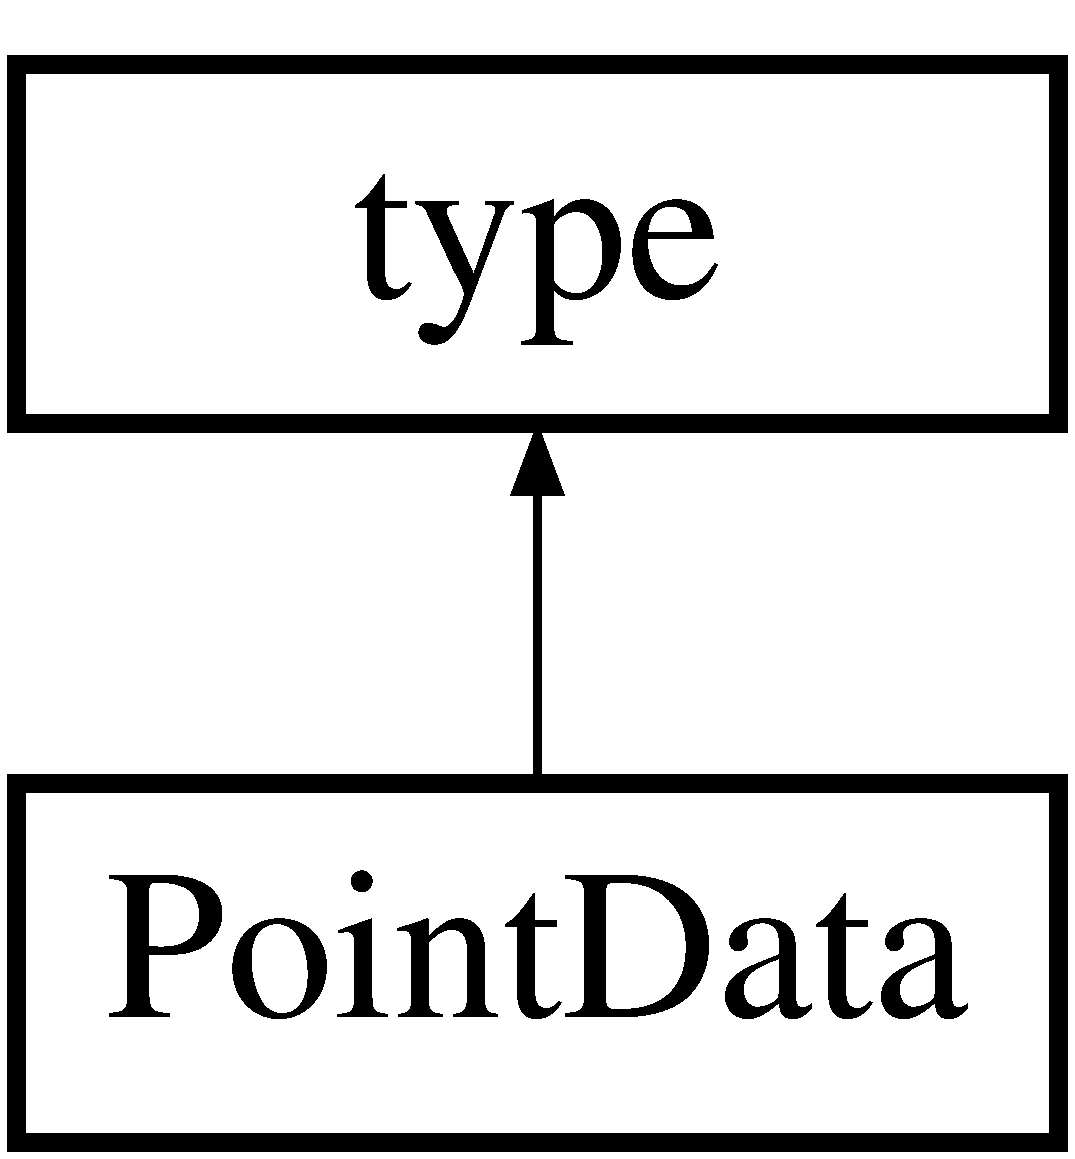
\includegraphics[height=2.000000cm]{classPointData}
\end{center}
\end{figure}
\subsection*{Public Types}
\begin{DoxyCompactItemize}
\item 
typedef \+::\hyperlink{classDataArray__t}{Data\+Array\+\_\+t} \hyperlink{classPointData_a249ad018361c7a9d61f42e1fc8af717f}{Data\+Array\+\_\+type}
\item 
typedef \+::xsd\+::cxx\+::tree\+::sequence$<$ \hyperlink{classPointData_a249ad018361c7a9d61f42e1fc8af717f}{Data\+Array\+\_\+type} $>$ \hyperlink{classPointData_acd882fa412789571fcaa2599ad2b2c71}{Data\+Array\+\_\+sequence}
\item 
typedef Data\+Array\+\_\+sequence\+::iterator \hyperlink{classPointData_afb66f793f2a65ca38e3cd8fa21eef701}{Data\+Array\+\_\+iterator}
\item 
typedef Data\+Array\+\_\+sequence\+::const\+\_\+iterator \hyperlink{classPointData_a6bd3313479b6a109e24bc9e7b306831b}{Data\+Array\+\_\+const\+\_\+iterator}
\item 
typedef \+::xsd\+::cxx\+::tree\+::traits$<$ \hyperlink{classPointData_a249ad018361c7a9d61f42e1fc8af717f}{Data\+Array\+\_\+type}, char $>$ \hyperlink{classPointData_ae9066a14984b6f7aa938ba2d58244055}{Data\+Array\+\_\+traits}
\end{DoxyCompactItemize}
\subsection*{Public Member Functions}
\begin{DoxyCompactItemize}
\item 
const \hyperlink{classPointData_acd882fa412789571fcaa2599ad2b2c71}{Data\+Array\+\_\+sequence} \& \hyperlink{classPointData_ac4d75ba2976d6acdaceb0b69f574e895}{Data\+Array} () const 
\item 
\hyperlink{classPointData_acd882fa412789571fcaa2599ad2b2c71}{Data\+Array\+\_\+sequence} \& \hyperlink{classPointData_aa8ff7ad5b2c1d99794d4b96e481138d2}{Data\+Array} ()
\item 
void \hyperlink{classPointData_a207059b73203faf8b3fec8659a9104e5}{Data\+Array} (const \hyperlink{classPointData_acd882fa412789571fcaa2599ad2b2c71}{Data\+Array\+\_\+sequence} \&s)
\item 
\hyperlink{classPointData_add74ef42ae2c48850449cd59e216111f}{Point\+Data} ()
\item 
\hyperlink{classPointData_ae0d2a9251b2690a28a04a96105874e45}{Point\+Data} (const \+::xercesc\+::\+D\+O\+M\+Element \&e,\+::\hyperlink{namespacexml__schema_a0612287d030cb2732d31a45b258fdc87}{xml\+\_\+schema\+::flags} f=0,\+::\hyperlink{namespacexml__schema_ada9aa30dc722e93ee2ed7243085402a5}{xml\+\_\+schema\+::container} $\ast$c=0)
\item 
\hyperlink{classPointData_a552557267dd3178a8e76be436b0709bc}{Point\+Data} (const \hyperlink{classPointData}{Point\+Data} \&x,\+::\hyperlink{namespacexml__schema_a0612287d030cb2732d31a45b258fdc87}{xml\+\_\+schema\+::flags} f=0,\+::\hyperlink{namespacexml__schema_ada9aa30dc722e93ee2ed7243085402a5}{xml\+\_\+schema\+::container} $\ast$c=0)
\item 
virtual \hyperlink{classPointData}{Point\+Data} $\ast$ \hyperlink{classPointData_aeb33ffedc35f8abc9ffd0d2f053c68ac}{\+\_\+clone} (\+::\hyperlink{namespacexml__schema_a0612287d030cb2732d31a45b258fdc87}{xml\+\_\+schema\+::flags} f=0,\+::\hyperlink{namespacexml__schema_ada9aa30dc722e93ee2ed7243085402a5}{xml\+\_\+schema\+::container} $\ast$c=0) const 
\item 
\hyperlink{classPointData}{Point\+Data} \& \hyperlink{classPointData_a3e175cdff950d602a53f4511df54abfd}{operator=} (const \hyperlink{classPointData}{Point\+Data} \&x)
\item 
virtual \hyperlink{classPointData_a53f701fd5abdb6105900c13f8282305e}{$\sim$\+Point\+Data} ()
\end{DoxyCompactItemize}
\subsection*{Protected Member Functions}
\begin{DoxyCompactItemize}
\item 
void \hyperlink{classPointData_a67ad25c5798d484eb8169a90fda2eac5}{parse} (\+::xsd\+::cxx\+::xml\+::dom\+::parser$<$ char $>$ \&,\+::\hyperlink{namespacexml__schema_a0612287d030cb2732d31a45b258fdc87}{xml\+\_\+schema\+::flags})
\end{DoxyCompactItemize}
\subsection*{Protected Attributes}
\begin{DoxyCompactItemize}
\item 
\hyperlink{classPointData_acd882fa412789571fcaa2599ad2b2c71}{Data\+Array\+\_\+sequence} \hyperlink{classPointData_ac8eb59ecb308a38ccd18bd6185e32a92}{Data\+Array\+\_\+}
\end{DoxyCompactItemize}


\subsection{Member Typedef Documentation}
\index{Point\+Data@{Point\+Data}!Data\+Array\+\_\+const\+\_\+iterator@{Data\+Array\+\_\+const\+\_\+iterator}}
\index{Data\+Array\+\_\+const\+\_\+iterator@{Data\+Array\+\_\+const\+\_\+iterator}!Point\+Data@{Point\+Data}}
\subsubsection[{\texorpdfstring{Data\+Array\+\_\+const\+\_\+iterator}{DataArray_const_iterator}}]{\setlength{\rightskip}{0pt plus 5cm}typedef Data\+Array\+\_\+sequence\+::const\+\_\+iterator {\bf Point\+Data\+::\+Data\+Array\+\_\+const\+\_\+iterator}}\hypertarget{classPointData_a6bd3313479b6a109e24bc9e7b306831b}{}\label{classPointData_a6bd3313479b6a109e24bc9e7b306831b}
\index{Point\+Data@{Point\+Data}!Data\+Array\+\_\+iterator@{Data\+Array\+\_\+iterator}}
\index{Data\+Array\+\_\+iterator@{Data\+Array\+\_\+iterator}!Point\+Data@{Point\+Data}}
\subsubsection[{\texorpdfstring{Data\+Array\+\_\+iterator}{DataArray_iterator}}]{\setlength{\rightskip}{0pt plus 5cm}typedef Data\+Array\+\_\+sequence\+::iterator {\bf Point\+Data\+::\+Data\+Array\+\_\+iterator}}\hypertarget{classPointData_afb66f793f2a65ca38e3cd8fa21eef701}{}\label{classPointData_afb66f793f2a65ca38e3cd8fa21eef701}
\index{Point\+Data@{Point\+Data}!Data\+Array\+\_\+sequence@{Data\+Array\+\_\+sequence}}
\index{Data\+Array\+\_\+sequence@{Data\+Array\+\_\+sequence}!Point\+Data@{Point\+Data}}
\subsubsection[{\texorpdfstring{Data\+Array\+\_\+sequence}{DataArray_sequence}}]{\setlength{\rightskip}{0pt plus 5cm}typedef \+::xsd\+::cxx\+::tree\+::sequence$<$ {\bf Data\+Array\+\_\+type} $>$ {\bf Point\+Data\+::\+Data\+Array\+\_\+sequence}}\hypertarget{classPointData_acd882fa412789571fcaa2599ad2b2c71}{}\label{classPointData_acd882fa412789571fcaa2599ad2b2c71}
\index{Point\+Data@{Point\+Data}!Data\+Array\+\_\+traits@{Data\+Array\+\_\+traits}}
\index{Data\+Array\+\_\+traits@{Data\+Array\+\_\+traits}!Point\+Data@{Point\+Data}}
\subsubsection[{\texorpdfstring{Data\+Array\+\_\+traits}{DataArray_traits}}]{\setlength{\rightskip}{0pt plus 5cm}typedef \+::xsd\+::cxx\+::tree\+::traits$<$ {\bf Data\+Array\+\_\+type}, char $>$ {\bf Point\+Data\+::\+Data\+Array\+\_\+traits}}\hypertarget{classPointData_ae9066a14984b6f7aa938ba2d58244055}{}\label{classPointData_ae9066a14984b6f7aa938ba2d58244055}
\index{Point\+Data@{Point\+Data}!Data\+Array\+\_\+type@{Data\+Array\+\_\+type}}
\index{Data\+Array\+\_\+type@{Data\+Array\+\_\+type}!Point\+Data@{Point\+Data}}
\subsubsection[{\texorpdfstring{Data\+Array\+\_\+type}{DataArray_type}}]{\setlength{\rightskip}{0pt plus 5cm}typedef \+::{\bf Data\+Array\+\_\+t} {\bf Point\+Data\+::\+Data\+Array\+\_\+type}}\hypertarget{classPointData_a249ad018361c7a9d61f42e1fc8af717f}{}\label{classPointData_a249ad018361c7a9d61f42e1fc8af717f}


\subsection{Constructor \& Destructor Documentation}
\index{Point\+Data@{Point\+Data}!Point\+Data@{Point\+Data}}
\index{Point\+Data@{Point\+Data}!Point\+Data@{Point\+Data}}
\subsubsection[{\texorpdfstring{Point\+Data()}{PointData()}}]{\setlength{\rightskip}{0pt plus 5cm}Point\+Data\+::\+Point\+Data (
\begin{DoxyParamCaption}
{}
\end{DoxyParamCaption}
)}\hypertarget{classPointData_add74ef42ae2c48850449cd59e216111f}{}\label{classPointData_add74ef42ae2c48850449cd59e216111f}
\index{Point\+Data@{Point\+Data}!Point\+Data@{Point\+Data}}
\index{Point\+Data@{Point\+Data}!Point\+Data@{Point\+Data}}
\subsubsection[{\texorpdfstring{Point\+Data(const \+::xercesc\+::\+D\+O\+M\+Element \&e,\+::xml\+\_\+schema\+::flags f=0,\+::xml\+\_\+schema\+::container $\ast$c=0)}{PointData(const ::xercesc::DOMElement &e,::xml_schema::flags f=0,::xml_schema::container *c=0)}}]{\setlength{\rightskip}{0pt plus 5cm}Point\+Data\+::\+Point\+Data (
\begin{DoxyParamCaption}
\item[{const \+::xercesc\+::\+D\+O\+M\+Element \&}]{e, }
\item[{\+::{\bf xml\+\_\+schema\+::flags}}]{f = {\ttfamily 0}, }
\item[{\+::{\bf xml\+\_\+schema\+::container} $\ast$}]{c = {\ttfamily 0}}
\end{DoxyParamCaption}
)}\hypertarget{classPointData_ae0d2a9251b2690a28a04a96105874e45}{}\label{classPointData_ae0d2a9251b2690a28a04a96105874e45}
\index{Point\+Data@{Point\+Data}!Point\+Data@{Point\+Data}}
\index{Point\+Data@{Point\+Data}!Point\+Data@{Point\+Data}}
\subsubsection[{\texorpdfstring{Point\+Data(const Point\+Data \&x,\+::xml\+\_\+schema\+::flags f=0,\+::xml\+\_\+schema\+::container $\ast$c=0)}{PointData(const PointData &x,::xml_schema::flags f=0,::xml_schema::container *c=0)}}]{\setlength{\rightskip}{0pt plus 5cm}Point\+Data\+::\+Point\+Data (
\begin{DoxyParamCaption}
\item[{const {\bf Point\+Data} \&}]{x, }
\item[{\+::{\bf xml\+\_\+schema\+::flags}}]{f = {\ttfamily 0}, }
\item[{\+::{\bf xml\+\_\+schema\+::container} $\ast$}]{c = {\ttfamily 0}}
\end{DoxyParamCaption}
)}\hypertarget{classPointData_a552557267dd3178a8e76be436b0709bc}{}\label{classPointData_a552557267dd3178a8e76be436b0709bc}
\index{Point\+Data@{Point\+Data}!````~Point\+Data@{$\sim$\+Point\+Data}}
\index{````~Point\+Data@{$\sim$\+Point\+Data}!Point\+Data@{Point\+Data}}
\subsubsection[{\texorpdfstring{$\sim$\+Point\+Data()}{~PointData()}}]{\setlength{\rightskip}{0pt plus 5cm}Point\+Data\+::$\sim$\+Point\+Data (
\begin{DoxyParamCaption}
{}
\end{DoxyParamCaption}
)\hspace{0.3cm}{\ttfamily [virtual]}}\hypertarget{classPointData_a53f701fd5abdb6105900c13f8282305e}{}\label{classPointData_a53f701fd5abdb6105900c13f8282305e}


\subsection{Member Function Documentation}
\index{Point\+Data@{Point\+Data}!\+\_\+clone@{\+\_\+clone}}
\index{\+\_\+clone@{\+\_\+clone}!Point\+Data@{Point\+Data}}
\subsubsection[{\texorpdfstring{\+\_\+clone(\+::xml\+\_\+schema\+::flags f=0,\+::xml\+\_\+schema\+::container $\ast$c=0) const }{_clone(::xml_schema::flags f=0,::xml_schema::container *c=0) const }}]{\setlength{\rightskip}{0pt plus 5cm}{\bf Point\+Data} $\ast$ Point\+Data\+::\+\_\+clone (
\begin{DoxyParamCaption}
\item[{\+::{\bf xml\+\_\+schema\+::flags}}]{f = {\ttfamily 0}, }
\item[{\+::{\bf xml\+\_\+schema\+::container} $\ast$}]{c = {\ttfamily 0}}
\end{DoxyParamCaption}
) const\hspace{0.3cm}{\ttfamily [virtual]}}\hypertarget{classPointData_aeb33ffedc35f8abc9ffd0d2f053c68ac}{}\label{classPointData_aeb33ffedc35f8abc9ffd0d2f053c68ac}
\index{Point\+Data@{Point\+Data}!Data\+Array@{Data\+Array}}
\index{Data\+Array@{Data\+Array}!Point\+Data@{Point\+Data}}
\subsubsection[{\texorpdfstring{Data\+Array() const }{DataArray() const }}]{\setlength{\rightskip}{0pt plus 5cm}const {\bf Point\+Data\+::\+Data\+Array\+\_\+sequence} \& Point\+Data\+::\+Data\+Array (
\begin{DoxyParamCaption}
{}
\end{DoxyParamCaption}
) const}\hypertarget{classPointData_ac4d75ba2976d6acdaceb0b69f574e895}{}\label{classPointData_ac4d75ba2976d6acdaceb0b69f574e895}
\index{Point\+Data@{Point\+Data}!Data\+Array@{Data\+Array}}
\index{Data\+Array@{Data\+Array}!Point\+Data@{Point\+Data}}
\subsubsection[{\texorpdfstring{Data\+Array()}{DataArray()}}]{\setlength{\rightskip}{0pt plus 5cm}{\bf Point\+Data\+::\+Data\+Array\+\_\+sequence} \& Point\+Data\+::\+Data\+Array (
\begin{DoxyParamCaption}
{}
\end{DoxyParamCaption}
)}\hypertarget{classPointData_aa8ff7ad5b2c1d99794d4b96e481138d2}{}\label{classPointData_aa8ff7ad5b2c1d99794d4b96e481138d2}
\index{Point\+Data@{Point\+Data}!Data\+Array@{Data\+Array}}
\index{Data\+Array@{Data\+Array}!Point\+Data@{Point\+Data}}
\subsubsection[{\texorpdfstring{Data\+Array(const Data\+Array\+\_\+sequence \&s)}{DataArray(const DataArray_sequence &s)}}]{\setlength{\rightskip}{0pt plus 5cm}void Point\+Data\+::\+Data\+Array (
\begin{DoxyParamCaption}
\item[{const {\bf Data\+Array\+\_\+sequence} \&}]{s}
\end{DoxyParamCaption}
)}\hypertarget{classPointData_a207059b73203faf8b3fec8659a9104e5}{}\label{classPointData_a207059b73203faf8b3fec8659a9104e5}
\index{Point\+Data@{Point\+Data}!operator=@{operator=}}
\index{operator=@{operator=}!Point\+Data@{Point\+Data}}
\subsubsection[{\texorpdfstring{operator=(const Point\+Data \&x)}{operator=(const PointData &x)}}]{\setlength{\rightskip}{0pt plus 5cm}{\bf Point\+Data} \& Point\+Data\+::operator= (
\begin{DoxyParamCaption}
\item[{const {\bf Point\+Data} \&}]{x}
\end{DoxyParamCaption}
)}\hypertarget{classPointData_a3e175cdff950d602a53f4511df54abfd}{}\label{classPointData_a3e175cdff950d602a53f4511df54abfd}
\index{Point\+Data@{Point\+Data}!parse@{parse}}
\index{parse@{parse}!Point\+Data@{Point\+Data}}
\subsubsection[{\texorpdfstring{parse(\+::xsd\+::cxx\+::xml\+::dom\+::parser$<$ char $>$ \&,\+::xml\+\_\+schema\+::flags)}{parse(::xsd::cxx::xml::dom::parser< char > &,::xml_schema::flags)}}]{\setlength{\rightskip}{0pt plus 5cm}void Point\+Data\+::parse (
\begin{DoxyParamCaption}
\item[{\+::xsd\+::cxx\+::xml\+::dom\+::parser$<$ char $>$ \&}]{p, }
\item[{\+::{\bf xml\+\_\+schema\+::flags}}]{f}
\end{DoxyParamCaption}
)\hspace{0.3cm}{\ttfamily [protected]}}\hypertarget{classPointData_a67ad25c5798d484eb8169a90fda2eac5}{}\label{classPointData_a67ad25c5798d484eb8169a90fda2eac5}


\subsection{Member Data Documentation}
\index{Point\+Data@{Point\+Data}!Data\+Array\+\_\+@{Data\+Array\+\_\+}}
\index{Data\+Array\+\_\+@{Data\+Array\+\_\+}!Point\+Data@{Point\+Data}}
\subsubsection[{\texorpdfstring{Data\+Array\+\_\+}{DataArray_}}]{\setlength{\rightskip}{0pt plus 5cm}{\bf Data\+Array\+\_\+sequence} Point\+Data\+::\+Data\+Array\+\_\+\hspace{0.3cm}{\ttfamily [protected]}}\hypertarget{classPointData_ac8eb59ecb308a38ccd18bd6185e32a92}{}\label{classPointData_ac8eb59ecb308a38ccd18bd6185e32a92}


The documentation for this class was generated from the following files\+:\begin{DoxyCompactItemize}
\item 
src/output\+Writer/\hyperlink{vtk-unstructured_8h}{vtk-\/unstructured.\+h}\item 
src/output\+Writer/\hyperlink{vtk-unstructured_8cpp}{vtk-\/unstructured.\+cpp}\end{DoxyCompactItemize}

\hypertarget{classPoints}{}\section{Points Class Reference}
\label{classPoints}\index{Points@{Points}}


{\ttfamily \#include $<$vtk-\/unstructured.\+h$>$}

Inheritance diagram for Points\+:\begin{figure}[H]
\begin{center}
\leavevmode
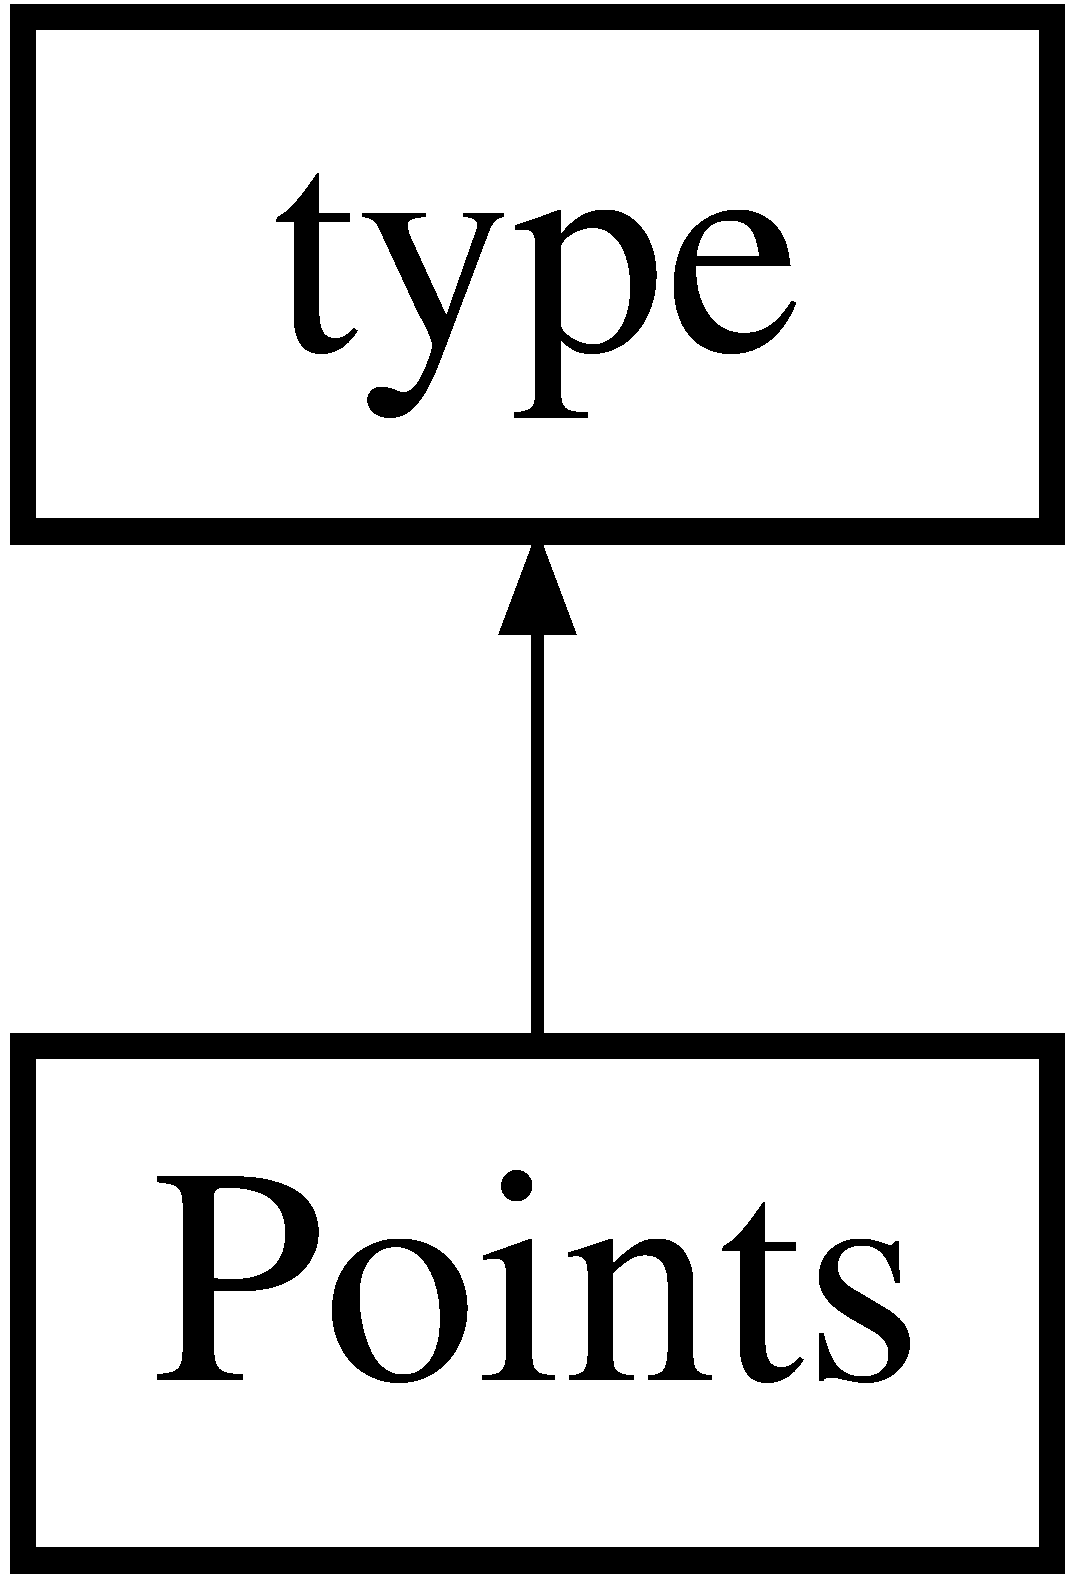
\includegraphics[height=2.000000cm]{classPoints}
\end{center}
\end{figure}
\subsection*{Public Types}
\begin{DoxyCompactItemize}
\item 
typedef \+::\hyperlink{classDataArray__t}{Data\+Array\+\_\+t} \hyperlink{classPoints_a6afedf501b722fe7d7ffeae03ece6238}{Data\+Array\+\_\+type}
\item 
typedef \+::xsd\+::cxx\+::tree\+::sequence$<$ \hyperlink{classPoints_a6afedf501b722fe7d7ffeae03ece6238}{Data\+Array\+\_\+type} $>$ \hyperlink{classPoints_ac8b51dcf0e7659ca61ff9b9d24051016}{Data\+Array\+\_\+sequence}
\item 
typedef Data\+Array\+\_\+sequence\+::iterator \hyperlink{classPoints_ac4cd7a177b464c1e08d493600a7e6e16}{Data\+Array\+\_\+iterator}
\item 
typedef Data\+Array\+\_\+sequence\+::const\+\_\+iterator \hyperlink{classPoints_a795a395909c3360569fe0e854ba6059e}{Data\+Array\+\_\+const\+\_\+iterator}
\item 
typedef \+::xsd\+::cxx\+::tree\+::traits$<$ \hyperlink{classPoints_a6afedf501b722fe7d7ffeae03ece6238}{Data\+Array\+\_\+type}, char $>$ \hyperlink{classPoints_a815b88c9204c7251f4a08c6769645ef1}{Data\+Array\+\_\+traits}
\end{DoxyCompactItemize}
\subsection*{Public Member Functions}
\begin{DoxyCompactItemize}
\item 
const \hyperlink{classPoints_ac8b51dcf0e7659ca61ff9b9d24051016}{Data\+Array\+\_\+sequence} \& \hyperlink{classPoints_a86c60a0068ebdb8d3e8cbe9fa8f35f55}{Data\+Array} () const 
\item 
\hyperlink{classPoints_ac8b51dcf0e7659ca61ff9b9d24051016}{Data\+Array\+\_\+sequence} \& \hyperlink{classPoints_a3fdfb1b1b2f1221ad50ba5087826177c}{Data\+Array} ()
\item 
void \hyperlink{classPoints_aa22a86fe31d5f903be59dda3de92bb67}{Data\+Array} (const \hyperlink{classPoints_ac8b51dcf0e7659ca61ff9b9d24051016}{Data\+Array\+\_\+sequence} \&s)
\item 
\hyperlink{classPoints_aa4e68083d98bd04233c9753dfe1e46ab}{Points} ()
\item 
\hyperlink{classPoints_a36a1ac8ea9ac092adff2888915e81304}{Points} (const \+::xercesc\+::\+D\+O\+M\+Element \&e,\+::\hyperlink{namespacexml__schema_a0612287d030cb2732d31a45b258fdc87}{xml\+\_\+schema\+::flags} f=0,\+::\hyperlink{namespacexml__schema_ada9aa30dc722e93ee2ed7243085402a5}{xml\+\_\+schema\+::container} $\ast$c=0)
\item 
\hyperlink{classPoints_ad49b51469dc53b028c244a88bd9fb08b}{Points} (const \hyperlink{classPoints}{Points} \&x,\+::\hyperlink{namespacexml__schema_a0612287d030cb2732d31a45b258fdc87}{xml\+\_\+schema\+::flags} f=0,\+::\hyperlink{namespacexml__schema_ada9aa30dc722e93ee2ed7243085402a5}{xml\+\_\+schema\+::container} $\ast$c=0)
\item 
virtual \hyperlink{classPoints}{Points} $\ast$ \hyperlink{classPoints_a5dff673c4b4a59465aee3ede80328ae9}{\+\_\+clone} (\+::\hyperlink{namespacexml__schema_a0612287d030cb2732d31a45b258fdc87}{xml\+\_\+schema\+::flags} f=0,\+::\hyperlink{namespacexml__schema_ada9aa30dc722e93ee2ed7243085402a5}{xml\+\_\+schema\+::container} $\ast$c=0) const 
\item 
\hyperlink{classPoints}{Points} \& \hyperlink{classPoints_abf6e94122cfc53e80543249d72cb87c2}{operator=} (const \hyperlink{classPoints}{Points} \&x)
\item 
virtual \hyperlink{classPoints_a9d56d7dc8b6a6f492e07d354eb379c12}{$\sim$\+Points} ()
\end{DoxyCompactItemize}
\subsection*{Protected Member Functions}
\begin{DoxyCompactItemize}
\item 
void \hyperlink{classPoints_a444657f907a3ae7bb2e36a6069501a3f}{parse} (\+::xsd\+::cxx\+::xml\+::dom\+::parser$<$ char $>$ \&,\+::\hyperlink{namespacexml__schema_a0612287d030cb2732d31a45b258fdc87}{xml\+\_\+schema\+::flags})
\end{DoxyCompactItemize}
\subsection*{Protected Attributes}
\begin{DoxyCompactItemize}
\item 
\hyperlink{classPoints_ac8b51dcf0e7659ca61ff9b9d24051016}{Data\+Array\+\_\+sequence} \hyperlink{classPoints_aaefb5f68ce6dbd9813458e3dfabca626}{Data\+Array\+\_\+}
\end{DoxyCompactItemize}


\subsection{Member Typedef Documentation}
\index{Points@{Points}!Data\+Array\+\_\+const\+\_\+iterator@{Data\+Array\+\_\+const\+\_\+iterator}}
\index{Data\+Array\+\_\+const\+\_\+iterator@{Data\+Array\+\_\+const\+\_\+iterator}!Points@{Points}}
\subsubsection[{\texorpdfstring{Data\+Array\+\_\+const\+\_\+iterator}{DataArray_const_iterator}}]{\setlength{\rightskip}{0pt plus 5cm}typedef Data\+Array\+\_\+sequence\+::const\+\_\+iterator {\bf Points\+::\+Data\+Array\+\_\+const\+\_\+iterator}}\hypertarget{classPoints_a795a395909c3360569fe0e854ba6059e}{}\label{classPoints_a795a395909c3360569fe0e854ba6059e}
\index{Points@{Points}!Data\+Array\+\_\+iterator@{Data\+Array\+\_\+iterator}}
\index{Data\+Array\+\_\+iterator@{Data\+Array\+\_\+iterator}!Points@{Points}}
\subsubsection[{\texorpdfstring{Data\+Array\+\_\+iterator}{DataArray_iterator}}]{\setlength{\rightskip}{0pt plus 5cm}typedef Data\+Array\+\_\+sequence\+::iterator {\bf Points\+::\+Data\+Array\+\_\+iterator}}\hypertarget{classPoints_ac4cd7a177b464c1e08d493600a7e6e16}{}\label{classPoints_ac4cd7a177b464c1e08d493600a7e6e16}
\index{Points@{Points}!Data\+Array\+\_\+sequence@{Data\+Array\+\_\+sequence}}
\index{Data\+Array\+\_\+sequence@{Data\+Array\+\_\+sequence}!Points@{Points}}
\subsubsection[{\texorpdfstring{Data\+Array\+\_\+sequence}{DataArray_sequence}}]{\setlength{\rightskip}{0pt plus 5cm}typedef \+::xsd\+::cxx\+::tree\+::sequence$<$ {\bf Data\+Array\+\_\+type} $>$ {\bf Points\+::\+Data\+Array\+\_\+sequence}}\hypertarget{classPoints_ac8b51dcf0e7659ca61ff9b9d24051016}{}\label{classPoints_ac8b51dcf0e7659ca61ff9b9d24051016}
\index{Points@{Points}!Data\+Array\+\_\+traits@{Data\+Array\+\_\+traits}}
\index{Data\+Array\+\_\+traits@{Data\+Array\+\_\+traits}!Points@{Points}}
\subsubsection[{\texorpdfstring{Data\+Array\+\_\+traits}{DataArray_traits}}]{\setlength{\rightskip}{0pt plus 5cm}typedef \+::xsd\+::cxx\+::tree\+::traits$<$ {\bf Data\+Array\+\_\+type}, char $>$ {\bf Points\+::\+Data\+Array\+\_\+traits}}\hypertarget{classPoints_a815b88c9204c7251f4a08c6769645ef1}{}\label{classPoints_a815b88c9204c7251f4a08c6769645ef1}
\index{Points@{Points}!Data\+Array\+\_\+type@{Data\+Array\+\_\+type}}
\index{Data\+Array\+\_\+type@{Data\+Array\+\_\+type}!Points@{Points}}
\subsubsection[{\texorpdfstring{Data\+Array\+\_\+type}{DataArray_type}}]{\setlength{\rightskip}{0pt plus 5cm}typedef \+::{\bf Data\+Array\+\_\+t} {\bf Points\+::\+Data\+Array\+\_\+type}}\hypertarget{classPoints_a6afedf501b722fe7d7ffeae03ece6238}{}\label{classPoints_a6afedf501b722fe7d7ffeae03ece6238}


\subsection{Constructor \& Destructor Documentation}
\index{Points@{Points}!Points@{Points}}
\index{Points@{Points}!Points@{Points}}
\subsubsection[{\texorpdfstring{Points()}{Points()}}]{\setlength{\rightskip}{0pt plus 5cm}Points\+::\+Points (
\begin{DoxyParamCaption}
{}
\end{DoxyParamCaption}
)}\hypertarget{classPoints_aa4e68083d98bd04233c9753dfe1e46ab}{}\label{classPoints_aa4e68083d98bd04233c9753dfe1e46ab}
\index{Points@{Points}!Points@{Points}}
\index{Points@{Points}!Points@{Points}}
\subsubsection[{\texorpdfstring{Points(const \+::xercesc\+::\+D\+O\+M\+Element \&e,\+::xml\+\_\+schema\+::flags f=0,\+::xml\+\_\+schema\+::container $\ast$c=0)}{Points(const ::xercesc::DOMElement &e,::xml_schema::flags f=0,::xml_schema::container *c=0)}}]{\setlength{\rightskip}{0pt plus 5cm}Points\+::\+Points (
\begin{DoxyParamCaption}
\item[{const \+::xercesc\+::\+D\+O\+M\+Element \&}]{e, }
\item[{\+::{\bf xml\+\_\+schema\+::flags}}]{f = {\ttfamily 0}, }
\item[{\+::{\bf xml\+\_\+schema\+::container} $\ast$}]{c = {\ttfamily 0}}
\end{DoxyParamCaption}
)}\hypertarget{classPoints_a36a1ac8ea9ac092adff2888915e81304}{}\label{classPoints_a36a1ac8ea9ac092adff2888915e81304}
\index{Points@{Points}!Points@{Points}}
\index{Points@{Points}!Points@{Points}}
\subsubsection[{\texorpdfstring{Points(const Points \&x,\+::xml\+\_\+schema\+::flags f=0,\+::xml\+\_\+schema\+::container $\ast$c=0)}{Points(const Points &x,::xml_schema::flags f=0,::xml_schema::container *c=0)}}]{\setlength{\rightskip}{0pt plus 5cm}Points\+::\+Points (
\begin{DoxyParamCaption}
\item[{const {\bf Points} \&}]{x, }
\item[{\+::{\bf xml\+\_\+schema\+::flags}}]{f = {\ttfamily 0}, }
\item[{\+::{\bf xml\+\_\+schema\+::container} $\ast$}]{c = {\ttfamily 0}}
\end{DoxyParamCaption}
)}\hypertarget{classPoints_ad49b51469dc53b028c244a88bd9fb08b}{}\label{classPoints_ad49b51469dc53b028c244a88bd9fb08b}
\index{Points@{Points}!````~Points@{$\sim$\+Points}}
\index{````~Points@{$\sim$\+Points}!Points@{Points}}
\subsubsection[{\texorpdfstring{$\sim$\+Points()}{~Points()}}]{\setlength{\rightskip}{0pt plus 5cm}Points\+::$\sim$\+Points (
\begin{DoxyParamCaption}
{}
\end{DoxyParamCaption}
)\hspace{0.3cm}{\ttfamily [virtual]}}\hypertarget{classPoints_a9d56d7dc8b6a6f492e07d354eb379c12}{}\label{classPoints_a9d56d7dc8b6a6f492e07d354eb379c12}


\subsection{Member Function Documentation}
\index{Points@{Points}!\+\_\+clone@{\+\_\+clone}}
\index{\+\_\+clone@{\+\_\+clone}!Points@{Points}}
\subsubsection[{\texorpdfstring{\+\_\+clone(\+::xml\+\_\+schema\+::flags f=0,\+::xml\+\_\+schema\+::container $\ast$c=0) const }{_clone(::xml_schema::flags f=0,::xml_schema::container *c=0) const }}]{\setlength{\rightskip}{0pt plus 5cm}{\bf Points} $\ast$ Points\+::\+\_\+clone (
\begin{DoxyParamCaption}
\item[{\+::{\bf xml\+\_\+schema\+::flags}}]{f = {\ttfamily 0}, }
\item[{\+::{\bf xml\+\_\+schema\+::container} $\ast$}]{c = {\ttfamily 0}}
\end{DoxyParamCaption}
) const\hspace{0.3cm}{\ttfamily [virtual]}}\hypertarget{classPoints_a5dff673c4b4a59465aee3ede80328ae9}{}\label{classPoints_a5dff673c4b4a59465aee3ede80328ae9}
\index{Points@{Points}!Data\+Array@{Data\+Array}}
\index{Data\+Array@{Data\+Array}!Points@{Points}}
\subsubsection[{\texorpdfstring{Data\+Array() const }{DataArray() const }}]{\setlength{\rightskip}{0pt plus 5cm}const {\bf Points\+::\+Data\+Array\+\_\+sequence} \& Points\+::\+Data\+Array (
\begin{DoxyParamCaption}
{}
\end{DoxyParamCaption}
) const}\hypertarget{classPoints_a86c60a0068ebdb8d3e8cbe9fa8f35f55}{}\label{classPoints_a86c60a0068ebdb8d3e8cbe9fa8f35f55}
\index{Points@{Points}!Data\+Array@{Data\+Array}}
\index{Data\+Array@{Data\+Array}!Points@{Points}}
\subsubsection[{\texorpdfstring{Data\+Array()}{DataArray()}}]{\setlength{\rightskip}{0pt plus 5cm}{\bf Points\+::\+Data\+Array\+\_\+sequence} \& Points\+::\+Data\+Array (
\begin{DoxyParamCaption}
{}
\end{DoxyParamCaption}
)}\hypertarget{classPoints_a3fdfb1b1b2f1221ad50ba5087826177c}{}\label{classPoints_a3fdfb1b1b2f1221ad50ba5087826177c}
\index{Points@{Points}!Data\+Array@{Data\+Array}}
\index{Data\+Array@{Data\+Array}!Points@{Points}}
\subsubsection[{\texorpdfstring{Data\+Array(const Data\+Array\+\_\+sequence \&s)}{DataArray(const DataArray_sequence &s)}}]{\setlength{\rightskip}{0pt plus 5cm}void Points\+::\+Data\+Array (
\begin{DoxyParamCaption}
\item[{const {\bf Data\+Array\+\_\+sequence} \&}]{s}
\end{DoxyParamCaption}
)}\hypertarget{classPoints_aa22a86fe31d5f903be59dda3de92bb67}{}\label{classPoints_aa22a86fe31d5f903be59dda3de92bb67}
\index{Points@{Points}!operator=@{operator=}}
\index{operator=@{operator=}!Points@{Points}}
\subsubsection[{\texorpdfstring{operator=(const Points \&x)}{operator=(const Points &x)}}]{\setlength{\rightskip}{0pt plus 5cm}{\bf Points} \& Points\+::operator= (
\begin{DoxyParamCaption}
\item[{const {\bf Points} \&}]{x}
\end{DoxyParamCaption}
)}\hypertarget{classPoints_abf6e94122cfc53e80543249d72cb87c2}{}\label{classPoints_abf6e94122cfc53e80543249d72cb87c2}
\index{Points@{Points}!parse@{parse}}
\index{parse@{parse}!Points@{Points}}
\subsubsection[{\texorpdfstring{parse(\+::xsd\+::cxx\+::xml\+::dom\+::parser$<$ char $>$ \&,\+::xml\+\_\+schema\+::flags)}{parse(::xsd::cxx::xml::dom::parser< char > &,::xml_schema::flags)}}]{\setlength{\rightskip}{0pt plus 5cm}void Points\+::parse (
\begin{DoxyParamCaption}
\item[{\+::xsd\+::cxx\+::xml\+::dom\+::parser$<$ char $>$ \&}]{p, }
\item[{\+::{\bf xml\+\_\+schema\+::flags}}]{f}
\end{DoxyParamCaption}
)\hspace{0.3cm}{\ttfamily [protected]}}\hypertarget{classPoints_a444657f907a3ae7bb2e36a6069501a3f}{}\label{classPoints_a444657f907a3ae7bb2e36a6069501a3f}


\subsection{Member Data Documentation}
\index{Points@{Points}!Data\+Array\+\_\+@{Data\+Array\+\_\+}}
\index{Data\+Array\+\_\+@{Data\+Array\+\_\+}!Points@{Points}}
\subsubsection[{\texorpdfstring{Data\+Array\+\_\+}{DataArray_}}]{\setlength{\rightskip}{0pt plus 5cm}{\bf Data\+Array\+\_\+sequence} Points\+::\+Data\+Array\+\_\+\hspace{0.3cm}{\ttfamily [protected]}}\hypertarget{classPoints_aaefb5f68ce6dbd9813458e3dfabca626}{}\label{classPoints_aaefb5f68ce6dbd9813458e3dfabca626}


The documentation for this class was generated from the following files\+:\begin{DoxyCompactItemize}
\item 
src/output\+Writer/\hyperlink{vtk-unstructured_8h}{vtk-\/unstructured.\+h}\item 
src/output\+Writer/\hyperlink{vtk-unstructured_8cpp}{vtk-\/unstructured.\+cpp}\end{DoxyCompactItemize}

\hypertarget{classPolyData__t}{}\section{Poly\+Data\+\_\+t Class Reference}
\label{classPolyData__t}\index{Poly\+Data\+\_\+t@{Poly\+Data\+\_\+t}}


{\ttfamily \#include $<$vtk-\/unstructured.\+h$>$}

Inheritance diagram for Poly\+Data\+\_\+t\+:\begin{figure}[H]
\begin{center}
\leavevmode
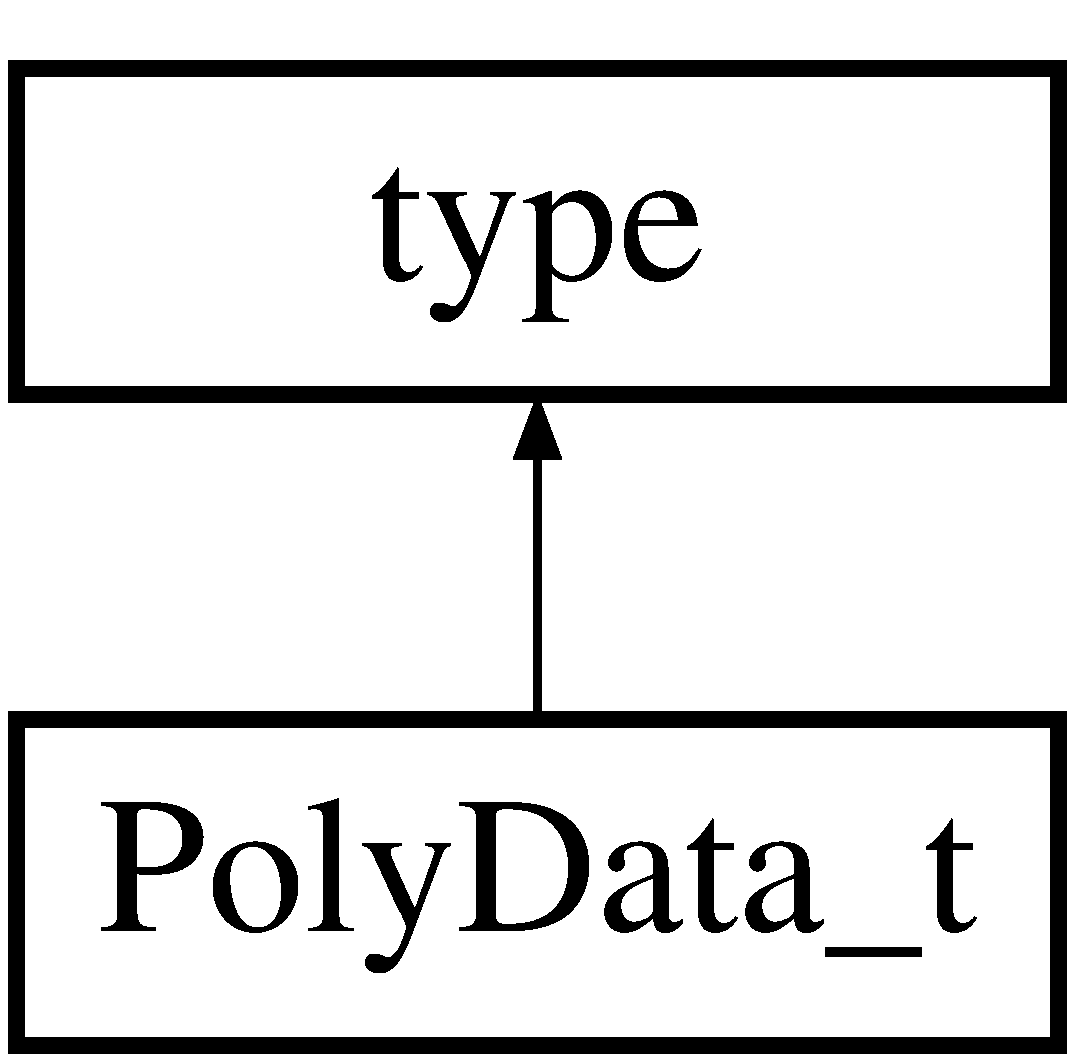
\includegraphics[height=2.000000cm]{classPolyData__t}
\end{center}
\end{figure}
\subsection*{Public Types}
\begin{DoxyCompactItemize}
\item 
typedef \+::\hyperlink{namespacexml__schema_ac0cec83a330f0024e4e318b3deac5104}{xml\+\_\+schema\+::string} \hyperlink{classPolyData__t_ae1f86bd7b6a37a0d0851de8a44627177}{greeting\+\_\+type}
\item 
typedef \+::xsd\+::cxx\+::tree\+::traits$<$ \hyperlink{classPolyData__t_ae1f86bd7b6a37a0d0851de8a44627177}{greeting\+\_\+type}, char $>$ \hyperlink{classPolyData__t_a0825d12eafceffcedbb147730b8bf8a6}{greeting\+\_\+traits}
\end{DoxyCompactItemize}
\subsection*{Public Member Functions}
\begin{DoxyCompactItemize}
\item 
const \hyperlink{classPolyData__t_ae1f86bd7b6a37a0d0851de8a44627177}{greeting\+\_\+type} \& \hyperlink{classPolyData__t_acce3e6cf99db0b383320a0ccfd62789f}{greeting} () const 
\item 
\hyperlink{classPolyData__t_ae1f86bd7b6a37a0d0851de8a44627177}{greeting\+\_\+type} \& \hyperlink{classPolyData__t_a3879d9f3b0b8ae707f1c2465bbbcf507}{greeting} ()
\item 
void \hyperlink{classPolyData__t_a23d6e1490860af1f76f135efb37510e1}{greeting} (const \hyperlink{classPolyData__t_ae1f86bd7b6a37a0d0851de8a44627177}{greeting\+\_\+type} \&x)
\item 
void \hyperlink{classPolyData__t_a25343d3827d7c4049d213c307b491406}{greeting} (\+::std\+::unique\+\_\+ptr$<$ \hyperlink{classPolyData__t_ae1f86bd7b6a37a0d0851de8a44627177}{greeting\+\_\+type} $>$ p)
\item 
\hyperlink{classPolyData__t_a4da6cc1205eee54feaebde53665f0621}{Poly\+Data\+\_\+t} (const \hyperlink{classPolyData__t_ae1f86bd7b6a37a0d0851de8a44627177}{greeting\+\_\+type} \&)
\item 
\hyperlink{classPolyData__t_a47b921cff0546cc9502c008a219d0058}{Poly\+Data\+\_\+t} (const \+::xercesc\+::\+D\+O\+M\+Element \&e,\+::\hyperlink{namespacexml__schema_a0612287d030cb2732d31a45b258fdc87}{xml\+\_\+schema\+::flags} f=0,\+::\hyperlink{namespacexml__schema_ada9aa30dc722e93ee2ed7243085402a5}{xml\+\_\+schema\+::container} $\ast$c=0)
\item 
\hyperlink{classPolyData__t_a6a0cccceec7668fe2f28776a4898a009}{Poly\+Data\+\_\+t} (const \hyperlink{classPolyData__t}{Poly\+Data\+\_\+t} \&x,\+::\hyperlink{namespacexml__schema_a0612287d030cb2732d31a45b258fdc87}{xml\+\_\+schema\+::flags} f=0,\+::\hyperlink{namespacexml__schema_ada9aa30dc722e93ee2ed7243085402a5}{xml\+\_\+schema\+::container} $\ast$c=0)
\item 
virtual \hyperlink{classPolyData__t}{Poly\+Data\+\_\+t} $\ast$ \hyperlink{classPolyData__t_a90079722e663d849db7dec71493ddffe}{\+\_\+clone} (\+::\hyperlink{namespacexml__schema_a0612287d030cb2732d31a45b258fdc87}{xml\+\_\+schema\+::flags} f=0,\+::\hyperlink{namespacexml__schema_ada9aa30dc722e93ee2ed7243085402a5}{xml\+\_\+schema\+::container} $\ast$c=0) const 
\item 
\hyperlink{classPolyData__t}{Poly\+Data\+\_\+t} \& \hyperlink{classPolyData__t_a8fe982e0bf8816c6f50e5d6a6c4a1d84}{operator=} (const \hyperlink{classPolyData__t}{Poly\+Data\+\_\+t} \&x)
\item 
virtual \hyperlink{classPolyData__t_afefe18d998d21a0557e30c06b4089b99}{$\sim$\+Poly\+Data\+\_\+t} ()
\end{DoxyCompactItemize}
\subsection*{Protected Member Functions}
\begin{DoxyCompactItemize}
\item 
void \hyperlink{classPolyData__t_a96ef26c9f46b47eb6e1206d1ef8d98b3}{parse} (\+::xsd\+::cxx\+::xml\+::dom\+::parser$<$ char $>$ \&,\+::\hyperlink{namespacexml__schema_a0612287d030cb2732d31a45b258fdc87}{xml\+\_\+schema\+::flags})
\end{DoxyCompactItemize}
\subsection*{Protected Attributes}
\begin{DoxyCompactItemize}
\item 
\+::xsd\+::cxx\+::tree\+::one$<$ \hyperlink{classPolyData__t_ae1f86bd7b6a37a0d0851de8a44627177}{greeting\+\_\+type} $>$ \hyperlink{classPolyData__t_ac266677696c0b4ad0a1a51d8ff6d3c04}{greeting\+\_\+}
\end{DoxyCompactItemize}


\subsection{Member Typedef Documentation}
\index{Poly\+Data\+\_\+t@{Poly\+Data\+\_\+t}!greeting\+\_\+traits@{greeting\+\_\+traits}}
\index{greeting\+\_\+traits@{greeting\+\_\+traits}!Poly\+Data\+\_\+t@{Poly\+Data\+\_\+t}}
\subsubsection[{\texorpdfstring{greeting\+\_\+traits}{greeting_traits}}]{\setlength{\rightskip}{0pt plus 5cm}typedef \+::xsd\+::cxx\+::tree\+::traits$<$ {\bf greeting\+\_\+type}, char $>$ {\bf Poly\+Data\+\_\+t\+::greeting\+\_\+traits}}\hypertarget{classPolyData__t_a0825d12eafceffcedbb147730b8bf8a6}{}\label{classPolyData__t_a0825d12eafceffcedbb147730b8bf8a6}
\index{Poly\+Data\+\_\+t@{Poly\+Data\+\_\+t}!greeting\+\_\+type@{greeting\+\_\+type}}
\index{greeting\+\_\+type@{greeting\+\_\+type}!Poly\+Data\+\_\+t@{Poly\+Data\+\_\+t}}
\subsubsection[{\texorpdfstring{greeting\+\_\+type}{greeting_type}}]{\setlength{\rightskip}{0pt plus 5cm}typedef \+::{\bf xml\+\_\+schema\+::string} {\bf Poly\+Data\+\_\+t\+::greeting\+\_\+type}}\hypertarget{classPolyData__t_ae1f86bd7b6a37a0d0851de8a44627177}{}\label{classPolyData__t_ae1f86bd7b6a37a0d0851de8a44627177}


\subsection{Constructor \& Destructor Documentation}
\index{Poly\+Data\+\_\+t@{Poly\+Data\+\_\+t}!Poly\+Data\+\_\+t@{Poly\+Data\+\_\+t}}
\index{Poly\+Data\+\_\+t@{Poly\+Data\+\_\+t}!Poly\+Data\+\_\+t@{Poly\+Data\+\_\+t}}
\subsubsection[{\texorpdfstring{Poly\+Data\+\_\+t(const greeting\+\_\+type \&)}{PolyData_t(const greeting_type &)}}]{\setlength{\rightskip}{0pt plus 5cm}Poly\+Data\+\_\+t\+::\+Poly\+Data\+\_\+t (
\begin{DoxyParamCaption}
\item[{const {\bf greeting\+\_\+type} \&}]{greeting}
\end{DoxyParamCaption}
)}\hypertarget{classPolyData__t_a4da6cc1205eee54feaebde53665f0621}{}\label{classPolyData__t_a4da6cc1205eee54feaebde53665f0621}
\index{Poly\+Data\+\_\+t@{Poly\+Data\+\_\+t}!Poly\+Data\+\_\+t@{Poly\+Data\+\_\+t}}
\index{Poly\+Data\+\_\+t@{Poly\+Data\+\_\+t}!Poly\+Data\+\_\+t@{Poly\+Data\+\_\+t}}
\subsubsection[{\texorpdfstring{Poly\+Data\+\_\+t(const \+::xercesc\+::\+D\+O\+M\+Element \&e,\+::xml\+\_\+schema\+::flags f=0,\+::xml\+\_\+schema\+::container $\ast$c=0)}{PolyData_t(const ::xercesc::DOMElement &e,::xml_schema::flags f=0,::xml_schema::container *c=0)}}]{\setlength{\rightskip}{0pt plus 5cm}Poly\+Data\+\_\+t\+::\+Poly\+Data\+\_\+t (
\begin{DoxyParamCaption}
\item[{const \+::xercesc\+::\+D\+O\+M\+Element \&}]{e, }
\item[{\+::{\bf xml\+\_\+schema\+::flags}}]{f = {\ttfamily 0}, }
\item[{\+::{\bf xml\+\_\+schema\+::container} $\ast$}]{c = {\ttfamily 0}}
\end{DoxyParamCaption}
)}\hypertarget{classPolyData__t_a47b921cff0546cc9502c008a219d0058}{}\label{classPolyData__t_a47b921cff0546cc9502c008a219d0058}
\index{Poly\+Data\+\_\+t@{Poly\+Data\+\_\+t}!Poly\+Data\+\_\+t@{Poly\+Data\+\_\+t}}
\index{Poly\+Data\+\_\+t@{Poly\+Data\+\_\+t}!Poly\+Data\+\_\+t@{Poly\+Data\+\_\+t}}
\subsubsection[{\texorpdfstring{Poly\+Data\+\_\+t(const Poly\+Data\+\_\+t \&x,\+::xml\+\_\+schema\+::flags f=0,\+::xml\+\_\+schema\+::container $\ast$c=0)}{PolyData_t(const PolyData_t &x,::xml_schema::flags f=0,::xml_schema::container *c=0)}}]{\setlength{\rightskip}{0pt plus 5cm}Poly\+Data\+\_\+t\+::\+Poly\+Data\+\_\+t (
\begin{DoxyParamCaption}
\item[{const {\bf Poly\+Data\+\_\+t} \&}]{x, }
\item[{\+::{\bf xml\+\_\+schema\+::flags}}]{f = {\ttfamily 0}, }
\item[{\+::{\bf xml\+\_\+schema\+::container} $\ast$}]{c = {\ttfamily 0}}
\end{DoxyParamCaption}
)}\hypertarget{classPolyData__t_a6a0cccceec7668fe2f28776a4898a009}{}\label{classPolyData__t_a6a0cccceec7668fe2f28776a4898a009}
\index{Poly\+Data\+\_\+t@{Poly\+Data\+\_\+t}!````~Poly\+Data\+\_\+t@{$\sim$\+Poly\+Data\+\_\+t}}
\index{````~Poly\+Data\+\_\+t@{$\sim$\+Poly\+Data\+\_\+t}!Poly\+Data\+\_\+t@{Poly\+Data\+\_\+t}}
\subsubsection[{\texorpdfstring{$\sim$\+Poly\+Data\+\_\+t()}{~PolyData_t()}}]{\setlength{\rightskip}{0pt plus 5cm}Poly\+Data\+\_\+t\+::$\sim$\+Poly\+Data\+\_\+t (
\begin{DoxyParamCaption}
{}
\end{DoxyParamCaption}
)\hspace{0.3cm}{\ttfamily [virtual]}}\hypertarget{classPolyData__t_afefe18d998d21a0557e30c06b4089b99}{}\label{classPolyData__t_afefe18d998d21a0557e30c06b4089b99}


\subsection{Member Function Documentation}
\index{Poly\+Data\+\_\+t@{Poly\+Data\+\_\+t}!\+\_\+clone@{\+\_\+clone}}
\index{\+\_\+clone@{\+\_\+clone}!Poly\+Data\+\_\+t@{Poly\+Data\+\_\+t}}
\subsubsection[{\texorpdfstring{\+\_\+clone(\+::xml\+\_\+schema\+::flags f=0,\+::xml\+\_\+schema\+::container $\ast$c=0) const }{_clone(::xml_schema::flags f=0,::xml_schema::container *c=0) const }}]{\setlength{\rightskip}{0pt plus 5cm}{\bf Poly\+Data\+\_\+t} $\ast$ Poly\+Data\+\_\+t\+::\+\_\+clone (
\begin{DoxyParamCaption}
\item[{\+::{\bf xml\+\_\+schema\+::flags}}]{f = {\ttfamily 0}, }
\item[{\+::{\bf xml\+\_\+schema\+::container} $\ast$}]{c = {\ttfamily 0}}
\end{DoxyParamCaption}
) const\hspace{0.3cm}{\ttfamily [virtual]}}\hypertarget{classPolyData__t_a90079722e663d849db7dec71493ddffe}{}\label{classPolyData__t_a90079722e663d849db7dec71493ddffe}
\index{Poly\+Data\+\_\+t@{Poly\+Data\+\_\+t}!greeting@{greeting}}
\index{greeting@{greeting}!Poly\+Data\+\_\+t@{Poly\+Data\+\_\+t}}
\subsubsection[{\texorpdfstring{greeting() const }{greeting() const }}]{\setlength{\rightskip}{0pt plus 5cm}const {\bf Poly\+Data\+\_\+t\+::greeting\+\_\+type} \& Poly\+Data\+\_\+t\+::greeting (
\begin{DoxyParamCaption}
{}
\end{DoxyParamCaption}
) const}\hypertarget{classPolyData__t_acce3e6cf99db0b383320a0ccfd62789f}{}\label{classPolyData__t_acce3e6cf99db0b383320a0ccfd62789f}
\index{Poly\+Data\+\_\+t@{Poly\+Data\+\_\+t}!greeting@{greeting}}
\index{greeting@{greeting}!Poly\+Data\+\_\+t@{Poly\+Data\+\_\+t}}
\subsubsection[{\texorpdfstring{greeting()}{greeting()}}]{\setlength{\rightskip}{0pt plus 5cm}{\bf Poly\+Data\+\_\+t\+::greeting\+\_\+type} \& Poly\+Data\+\_\+t\+::greeting (
\begin{DoxyParamCaption}
{}
\end{DoxyParamCaption}
)}\hypertarget{classPolyData__t_a3879d9f3b0b8ae707f1c2465bbbcf507}{}\label{classPolyData__t_a3879d9f3b0b8ae707f1c2465bbbcf507}
\index{Poly\+Data\+\_\+t@{Poly\+Data\+\_\+t}!greeting@{greeting}}
\index{greeting@{greeting}!Poly\+Data\+\_\+t@{Poly\+Data\+\_\+t}}
\subsubsection[{\texorpdfstring{greeting(const greeting\+\_\+type \&x)}{greeting(const greeting_type &x)}}]{\setlength{\rightskip}{0pt plus 5cm}void Poly\+Data\+\_\+t\+::greeting (
\begin{DoxyParamCaption}
\item[{const {\bf greeting\+\_\+type} \&}]{x}
\end{DoxyParamCaption}
)}\hypertarget{classPolyData__t_a23d6e1490860af1f76f135efb37510e1}{}\label{classPolyData__t_a23d6e1490860af1f76f135efb37510e1}
\index{Poly\+Data\+\_\+t@{Poly\+Data\+\_\+t}!greeting@{greeting}}
\index{greeting@{greeting}!Poly\+Data\+\_\+t@{Poly\+Data\+\_\+t}}
\subsubsection[{\texorpdfstring{greeting(\+::std\+::unique\+\_\+ptr$<$ greeting\+\_\+type $>$ p)}{greeting(::std::unique_ptr< greeting_type > p)}}]{\setlength{\rightskip}{0pt plus 5cm}void Poly\+Data\+\_\+t\+::greeting (
\begin{DoxyParamCaption}
\item[{\+::std\+::unique\+\_\+ptr$<$ {\bf greeting\+\_\+type} $>$}]{p}
\end{DoxyParamCaption}
)}\hypertarget{classPolyData__t_a25343d3827d7c4049d213c307b491406}{}\label{classPolyData__t_a25343d3827d7c4049d213c307b491406}
\index{Poly\+Data\+\_\+t@{Poly\+Data\+\_\+t}!operator=@{operator=}}
\index{operator=@{operator=}!Poly\+Data\+\_\+t@{Poly\+Data\+\_\+t}}
\subsubsection[{\texorpdfstring{operator=(const Poly\+Data\+\_\+t \&x)}{operator=(const PolyData_t &x)}}]{\setlength{\rightskip}{0pt plus 5cm}{\bf Poly\+Data\+\_\+t} \& Poly\+Data\+\_\+t\+::operator= (
\begin{DoxyParamCaption}
\item[{const {\bf Poly\+Data\+\_\+t} \&}]{x}
\end{DoxyParamCaption}
)}\hypertarget{classPolyData__t_a8fe982e0bf8816c6f50e5d6a6c4a1d84}{}\label{classPolyData__t_a8fe982e0bf8816c6f50e5d6a6c4a1d84}
\index{Poly\+Data\+\_\+t@{Poly\+Data\+\_\+t}!parse@{parse}}
\index{parse@{parse}!Poly\+Data\+\_\+t@{Poly\+Data\+\_\+t}}
\subsubsection[{\texorpdfstring{parse(\+::xsd\+::cxx\+::xml\+::dom\+::parser$<$ char $>$ \&,\+::xml\+\_\+schema\+::flags)}{parse(::xsd::cxx::xml::dom::parser< char > &,::xml_schema::flags)}}]{\setlength{\rightskip}{0pt plus 5cm}void Poly\+Data\+\_\+t\+::parse (
\begin{DoxyParamCaption}
\item[{\+::xsd\+::cxx\+::xml\+::dom\+::parser$<$ char $>$ \&}]{p, }
\item[{\+::{\bf xml\+\_\+schema\+::flags}}]{f}
\end{DoxyParamCaption}
)\hspace{0.3cm}{\ttfamily [protected]}}\hypertarget{classPolyData__t_a96ef26c9f46b47eb6e1206d1ef8d98b3}{}\label{classPolyData__t_a96ef26c9f46b47eb6e1206d1ef8d98b3}


\subsection{Member Data Documentation}
\index{Poly\+Data\+\_\+t@{Poly\+Data\+\_\+t}!greeting\+\_\+@{greeting\+\_\+}}
\index{greeting\+\_\+@{greeting\+\_\+}!Poly\+Data\+\_\+t@{Poly\+Data\+\_\+t}}
\subsubsection[{\texorpdfstring{greeting\+\_\+}{greeting_}}]{\setlength{\rightskip}{0pt plus 5cm}\+::xsd\+::cxx\+::tree\+::one$<$ {\bf greeting\+\_\+type} $>$ Poly\+Data\+\_\+t\+::greeting\+\_\+\hspace{0.3cm}{\ttfamily [protected]}}\hypertarget{classPolyData__t_ac266677696c0b4ad0a1a51d8ff6d3c04}{}\label{classPolyData__t_ac266677696c0b4ad0a1a51d8ff6d3c04}


The documentation for this class was generated from the following files\+:\begin{DoxyCompactItemize}
\item 
src/output\+Writer/\hyperlink{vtk-unstructured_8h}{vtk-\/unstructured.\+h}\item 
src/output\+Writer/\hyperlink{vtk-unstructured_8cpp}{vtk-\/unstructured.\+cpp}\end{DoxyCompactItemize}

\hypertarget{classsetting__t}{}\section{setting\+\_\+t Class Reference}
\label{classsetting__t}\index{setting\+\_\+t@{setting\+\_\+t}}


{\ttfamily \#include $<$setting.\+h$>$}

Inheritance diagram for setting\+\_\+t\+:\begin{figure}[H]
\begin{center}
\leavevmode
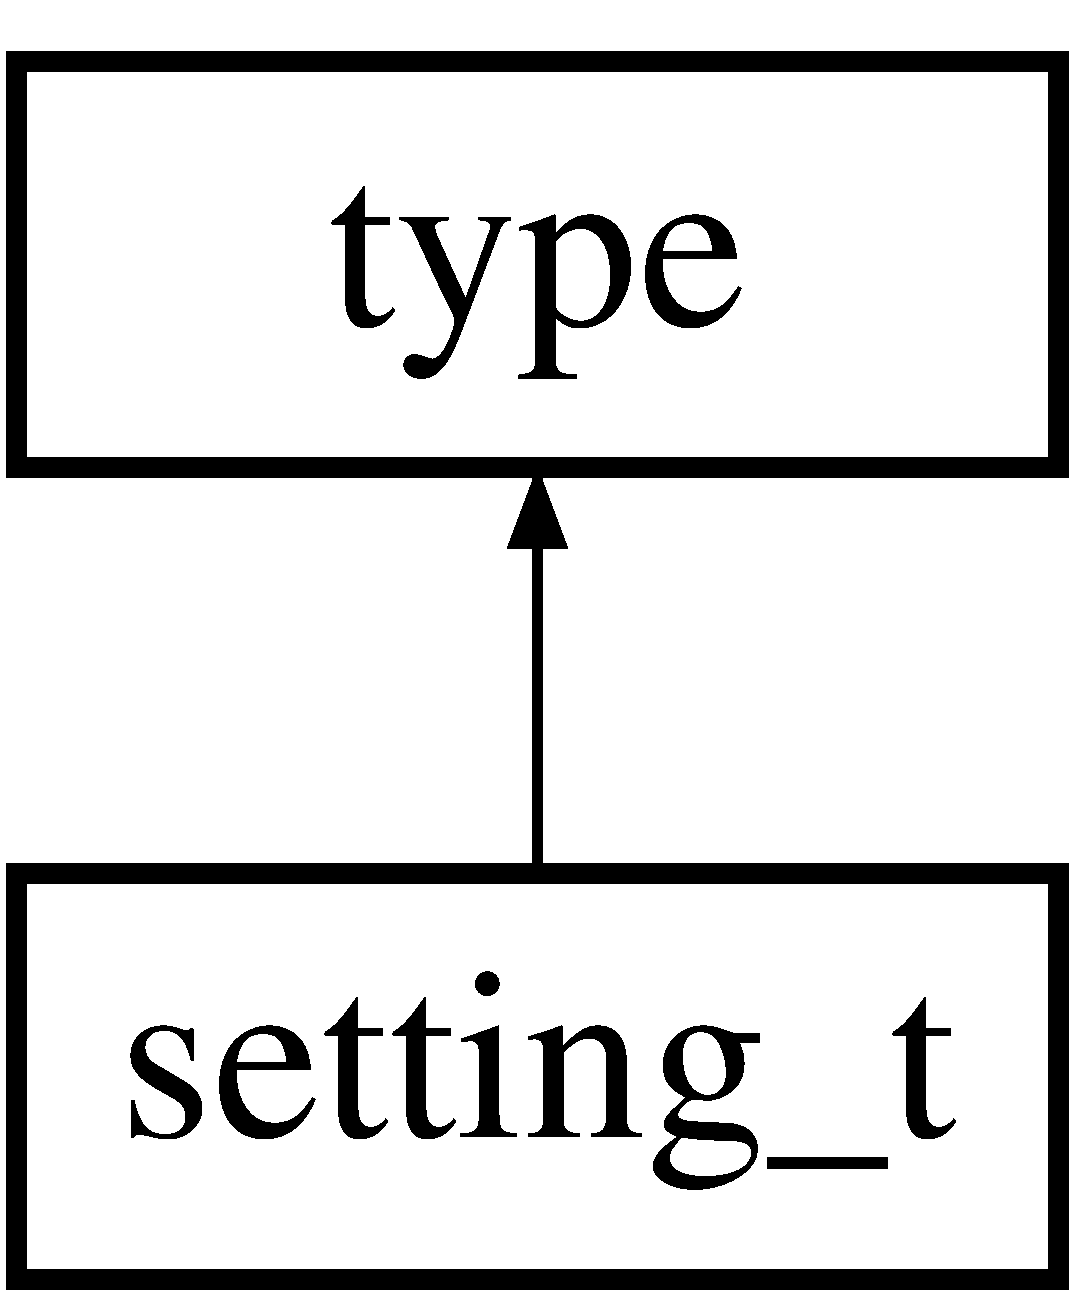
\includegraphics[height=2.000000cm]{classsetting__t}
\end{center}
\end{figure}
\subsection*{Public Types}
\begin{DoxyCompactItemize}
\item 
typedef \+::\hyperlink{namespacexml__schema_ac0cec83a330f0024e4e318b3deac5104}{xml\+\_\+schema\+::string} \hyperlink{classsetting__t_a176d76dc9ab1b149c679035ce0aa5448}{outputname\+\_\+type}
\item 
typedef \+::xsd\+::cxx\+::tree\+::traits$<$ \hyperlink{classsetting__t_a176d76dc9ab1b149c679035ce0aa5448}{outputname\+\_\+type}, char $>$ \hyperlink{classsetting__t_ae26e11d5332e659cec4e08d78cd65bbd}{outputname\+\_\+traits}
\item 
typedef \+::\hyperlink{namespacexml__schema_ac0cec83a330f0024e4e318b3deac5104}{xml\+\_\+schema\+::string} \hyperlink{classsetting__t_a395877994cdfcf2ea063a56aed90cf01}{endfile\+\_\+type}
\item 
typedef \+::xsd\+::cxx\+::tree\+::optional$<$ \hyperlink{classsetting__t_a395877994cdfcf2ea063a56aed90cf01}{endfile\+\_\+type} $>$ \hyperlink{classsetting__t_a38dbb691ee80d982dc24fd1b3e514f1e}{endfile\+\_\+optional}
\item 
typedef \+::xsd\+::cxx\+::tree\+::traits$<$ \hyperlink{classsetting__t_a395877994cdfcf2ea063a56aed90cf01}{endfile\+\_\+type}, char $>$ \hyperlink{classsetting__t_a0c2240e9363329e936e3ba35fa9ec642}{endfile\+\_\+traits}
\item 
typedef \+::\hyperlink{namespacexml__schema_acfa24ac68e1a188e7f44c36f7a158bf4}{xml\+\_\+schema\+::int\+\_\+} \hyperlink{classsetting__t_af0353930c8d9e0e19ee57943f2d130ee}{frequency\+\_\+type}
\item 
typedef \+::xsd\+::cxx\+::tree\+::traits$<$ \hyperlink{classsetting__t_af0353930c8d9e0e19ee57943f2d130ee}{frequency\+\_\+type}, char $>$ \hyperlink{classsetting__t_a948d945ce65d7779e6820f6de48d0613}{frequency\+\_\+traits}
\item 
typedef \+::\hyperlink{namespacexml__schema_ac0cec83a330f0024e4e318b3deac5104}{xml\+\_\+schema\+::string} \hyperlink{classsetting__t_afaef422486c04366dea99f1c838feb59}{profile\+File\+\_\+type}
\item 
typedef \+::xsd\+::cxx\+::tree\+::optional$<$ \hyperlink{classsetting__t_afaef422486c04366dea99f1c838feb59}{profile\+File\+\_\+type} $>$ \hyperlink{classsetting__t_a9fc7a23427369cf0af6e4521b9e88d64}{profile\+File\+\_\+optional}
\item 
typedef \+::xsd\+::cxx\+::tree\+::traits$<$ \hyperlink{classsetting__t_afaef422486c04366dea99f1c838feb59}{profile\+File\+\_\+type}, char $>$ \hyperlink{classsetting__t_af0663c89478aa719ca80575a0f8f0585}{profile\+File\+\_\+traits}
\item 
typedef \+::\hyperlink{namespacexml__schema_acfa24ac68e1a188e7f44c36f7a158bf4}{xml\+\_\+schema\+::int\+\_\+} \hyperlink{classsetting__t_a424aba4ecbd3f03a202ef656303091a3}{profile\+Buckets\+X\+\_\+type}
\item 
typedef \+::xsd\+::cxx\+::tree\+::optional$<$ \hyperlink{classsetting__t_a424aba4ecbd3f03a202ef656303091a3}{profile\+Buckets\+X\+\_\+type} $>$ \hyperlink{classsetting__t_abe44e9ac5bfb035f396dc36d8a9831d6}{profile\+Buckets\+X\+\_\+optional}
\item 
typedef \+::xsd\+::cxx\+::tree\+::traits$<$ \hyperlink{classsetting__t_a424aba4ecbd3f03a202ef656303091a3}{profile\+Buckets\+X\+\_\+type}, char $>$ \hyperlink{classsetting__t_a2c2047f66bf736cf0d85fe515c715427}{profile\+Buckets\+X\+\_\+traits}
\item 
typedef \+::\hyperlink{namespacexml__schema_ad7e04ab17bba0b3fdde43fb79ef6ed87}{xml\+\_\+schema\+::float\+\_\+} \hyperlink{classsetting__t_ad2336c5ecdc0977272ba8126243d7977}{delta\+\_\+t\+\_\+type}
\item 
typedef \+::xsd\+::cxx\+::tree\+::traits$<$ \hyperlink{classsetting__t_ad2336c5ecdc0977272ba8126243d7977}{delta\+\_\+t\+\_\+type}, char $>$ \hyperlink{classsetting__t_a16a46f4b3724acbc577a9a89691709dd}{delta\+\_\+t\+\_\+traits}
\item 
typedef \+::\hyperlink{namespacexml__schema_ad7e04ab17bba0b3fdde43fb79ef6ed87}{xml\+\_\+schema\+::float\+\_\+} \hyperlink{classsetting__t_ab27962fdbca01941c3b6c632bc7ac360}{t\+\_\+end\+\_\+type}
\item 
typedef \+::xsd\+::cxx\+::tree\+::traits$<$ \hyperlink{classsetting__t_ab27962fdbca01941c3b6c632bc7ac360}{t\+\_\+end\+\_\+type}, char $>$ \hyperlink{classsetting__t_ab0900ed5312404537577df0234ed3239}{t\+\_\+end\+\_\+traits}
\item 
typedef \+::\hyperlink{namespacexml__schema_ad7e04ab17bba0b3fdde43fb79ef6ed87}{xml\+\_\+schema\+::float\+\_\+} \hyperlink{classsetting__t_afd5541e25ce3565005acb9c70bddda2d}{b\+\_\+factor\+\_\+type}
\item 
typedef \+::xsd\+::cxx\+::tree\+::traits$<$ \hyperlink{classsetting__t_afd5541e25ce3565005acb9c70bddda2d}{b\+\_\+factor\+\_\+type}, char $>$ \hyperlink{classsetting__t_a537558160cc066cde0fb14b74062cbf4}{b\+\_\+factor\+\_\+traits}
\item 
typedef \+::\hyperlink{namespacexml__schema_ad7e04ab17bba0b3fdde43fb79ef6ed87}{xml\+\_\+schema\+::float\+\_\+} \hyperlink{classsetting__t_af2a0b22be63f361de8ba6df7313b1a68}{g\+\_\+grav\+\_\+x\+\_\+type}
\item 
typedef \+::xsd\+::cxx\+::tree\+::traits$<$ \hyperlink{classsetting__t_af2a0b22be63f361de8ba6df7313b1a68}{g\+\_\+grav\+\_\+x\+\_\+type}, char $>$ \hyperlink{classsetting__t_a6a6c41b916afaf5875cef8b3725c41cf}{g\+\_\+grav\+\_\+x\+\_\+traits}
\item 
typedef \+::\hyperlink{namespacexml__schema_ad7e04ab17bba0b3fdde43fb79ef6ed87}{xml\+\_\+schema\+::float\+\_\+} \hyperlink{classsetting__t_a89b3c653de2dc5afa902042e34939589}{g\+\_\+grav\+\_\+y\+\_\+type}
\item 
typedef \+::xsd\+::cxx\+::tree\+::traits$<$ \hyperlink{classsetting__t_a89b3c653de2dc5afa902042e34939589}{g\+\_\+grav\+\_\+y\+\_\+type}, char $>$ \hyperlink{classsetting__t_ae11d083a1b0c3194a4295bdc5fd79a32}{g\+\_\+grav\+\_\+y\+\_\+traits}
\item 
typedef \+::\hyperlink{namespacexml__schema_ad7e04ab17bba0b3fdde43fb79ef6ed87}{xml\+\_\+schema\+::float\+\_\+} \hyperlink{classsetting__t_a2a9e06e642160debeeadb7a76b97c753}{g\+\_\+grav\+\_\+z\+\_\+type}
\item 
typedef \+::xsd\+::cxx\+::tree\+::traits$<$ \hyperlink{classsetting__t_a2a9e06e642160debeeadb7a76b97c753}{g\+\_\+grav\+\_\+z\+\_\+type}, char $>$ \hyperlink{classsetting__t_ab6a6497ea3d399fee80102fc84d04397}{g\+\_\+grav\+\_\+z\+\_\+traits}
\item 
typedef \+::\hyperlink{namespacexml__schema_ad7e04ab17bba0b3fdde43fb79ef6ed87}{xml\+\_\+schema\+::float\+\_\+} \hyperlink{classsetting__t_a1bf57fd62042e86d0e1e66f34fbaed31}{domain\+X\+\_\+type}
\item 
typedef \+::xsd\+::cxx\+::tree\+::traits$<$ \hyperlink{classsetting__t_a1bf57fd62042e86d0e1e66f34fbaed31}{domain\+X\+\_\+type}, char $>$ \hyperlink{classsetting__t_ab34396042c375f062bd2d6f062e15e67}{domain\+X\+\_\+traits}
\item 
typedef \+::\hyperlink{namespacexml__schema_ad7e04ab17bba0b3fdde43fb79ef6ed87}{xml\+\_\+schema\+::float\+\_\+} \hyperlink{classsetting__t_a9f13bfe9cc42660cf1e89cff4afe9435}{domain\+Y\+\_\+type}
\item 
typedef \+::xsd\+::cxx\+::tree\+::traits$<$ \hyperlink{classsetting__t_a9f13bfe9cc42660cf1e89cff4afe9435}{domain\+Y\+\_\+type}, char $>$ \hyperlink{classsetting__t_a9c732c5a7483b203f6f456a57de341ed}{domain\+Y\+\_\+traits}
\item 
typedef \+::\hyperlink{namespacexml__schema_ad7e04ab17bba0b3fdde43fb79ef6ed87}{xml\+\_\+schema\+::float\+\_\+} \hyperlink{classsetting__t_a2257367cc1475e2a9b1b2a82dbdaddaf}{domain\+Z\+\_\+type}
\item 
typedef \+::xsd\+::cxx\+::tree\+::traits$<$ \hyperlink{classsetting__t_a2257367cc1475e2a9b1b2a82dbdaddaf}{domain\+Z\+\_\+type}, char $>$ \hyperlink{classsetting__t_a9247da64df3be9ea926998c19eb16349}{domain\+Z\+\_\+traits}
\item 
typedef \+::\hyperlink{namespacexml__schema_ad7e04ab17bba0b3fdde43fb79ef6ed87}{xml\+\_\+schema\+::float\+\_\+} \hyperlink{classsetting__t_ac5da16857addda387f3269e0a1a0cafa}{r\+\_\+cutoff\+\_\+type}
\item 
typedef \+::xsd\+::cxx\+::tree\+::traits$<$ \hyperlink{classsetting__t_ac5da16857addda387f3269e0a1a0cafa}{r\+\_\+cutoff\+\_\+type}, char $>$ \hyperlink{classsetting__t_add5ef63c1e740878483b913818829da3}{r\+\_\+cutoff\+\_\+traits}
\item 
typedef \+::\hyperlink{namespacexml__schema_acfa24ac68e1a188e7f44c36f7a158bf4}{xml\+\_\+schema\+::int\+\_\+} \hyperlink{classsetting__t_a182532ef9d6146add054e0118af040f2}{bc\+\_\+left\+\_\+type}
\item 
typedef \+::xsd\+::cxx\+::tree\+::traits$<$ \hyperlink{classsetting__t_a182532ef9d6146add054e0118af040f2}{bc\+\_\+left\+\_\+type}, char $>$ \hyperlink{classsetting__t_a1618c9945b34bcf5522be0925ad0b6b7}{bc\+\_\+left\+\_\+traits}
\item 
typedef \+::\hyperlink{namespacexml__schema_acfa24ac68e1a188e7f44c36f7a158bf4}{xml\+\_\+schema\+::int\+\_\+} \hyperlink{classsetting__t_abf5df957f10853c7b6a54a0073cd61fa}{bc\+\_\+upper\+\_\+type}
\item 
typedef \+::xsd\+::cxx\+::tree\+::traits$<$ \hyperlink{classsetting__t_abf5df957f10853c7b6a54a0073cd61fa}{bc\+\_\+upper\+\_\+type}, char $>$ \hyperlink{classsetting__t_add475d3af08f63aab575ec9a5b2ef6b6}{bc\+\_\+upper\+\_\+traits}
\item 
typedef \+::\hyperlink{namespacexml__schema_acfa24ac68e1a188e7f44c36f7a158bf4}{xml\+\_\+schema\+::int\+\_\+} \hyperlink{classsetting__t_a958fcc958aca728509db3a1f3756a0c9}{bc\+\_\+right\+\_\+type}
\item 
typedef \+::xsd\+::cxx\+::tree\+::traits$<$ \hyperlink{classsetting__t_a958fcc958aca728509db3a1f3756a0c9}{bc\+\_\+right\+\_\+type}, char $>$ \hyperlink{classsetting__t_abe4962aa498bbe5c5289cc8ba26dbd8e}{bc\+\_\+right\+\_\+traits}
\item 
typedef \+::\hyperlink{namespacexml__schema_acfa24ac68e1a188e7f44c36f7a158bf4}{xml\+\_\+schema\+::int\+\_\+} \hyperlink{classsetting__t_a69864ad49075236ce00f2a73cdcbb13b}{bc\+\_\+lower\+\_\+type}
\item 
typedef \+::xsd\+::cxx\+::tree\+::traits$<$ \hyperlink{classsetting__t_a69864ad49075236ce00f2a73cdcbb13b}{bc\+\_\+lower\+\_\+type}, char $>$ \hyperlink{classsetting__t_a59114f8a8f73c5064628778c0e1cb9d5}{bc\+\_\+lower\+\_\+traits}
\item 
typedef \+::\hyperlink{namespacexml__schema_acfa24ac68e1a188e7f44c36f7a158bf4}{xml\+\_\+schema\+::int\+\_\+} \hyperlink{classsetting__t_a6010c9a9fc3ce2a4d583aa4bf07f650c}{bc\+\_\+front\+\_\+type}
\item 
typedef \+::xsd\+::cxx\+::tree\+::traits$<$ \hyperlink{classsetting__t_a6010c9a9fc3ce2a4d583aa4bf07f650c}{bc\+\_\+front\+\_\+type}, char $>$ \hyperlink{classsetting__t_a371a2bd08322094079d3ff5fbebf6add}{bc\+\_\+front\+\_\+traits}
\item 
typedef \+::\hyperlink{namespacexml__schema_acfa24ac68e1a188e7f44c36f7a158bf4}{xml\+\_\+schema\+::int\+\_\+} \hyperlink{classsetting__t_a5deb32969da7832b53abbf0564142627}{bc\+\_\+back\+\_\+type}
\item 
typedef \+::xsd\+::cxx\+::tree\+::traits$<$ \hyperlink{classsetting__t_a5deb32969da7832b53abbf0564142627}{bc\+\_\+back\+\_\+type}, char $>$ \hyperlink{classsetting__t_a5edb994d60080ec2324d0bfaec5d017f}{bc\+\_\+back\+\_\+traits}
\item 
typedef \+::\hyperlink{namespacexml__schema_ac0cec83a330f0024e4e318b3deac5104}{xml\+\_\+schema\+::string} \hyperlink{classsetting__t_a9775dbebbc97cf7465126aa14870147d}{inputfiles\+\_\+type}
\item 
typedef \+::xsd\+::cxx\+::tree\+::sequence$<$ \hyperlink{classsetting__t_a9775dbebbc97cf7465126aa14870147d}{inputfiles\+\_\+type} $>$ \hyperlink{classsetting__t_a7f069827c89edb95e2b4347f1484b7b3}{inputfiles\+\_\+sequence}
\item 
typedef inputfiles\+\_\+sequence\+::iterator \hyperlink{classsetting__t_aba5818f4d041a7e5fd85bc8dbad26cf6}{inputfiles\+\_\+iterator}
\item 
typedef inputfiles\+\_\+sequence\+::const\+\_\+iterator \hyperlink{classsetting__t_ae3c8f20640b10bda631423b7a7992d96}{inputfiles\+\_\+const\+\_\+iterator}
\item 
typedef \+::xsd\+::cxx\+::tree\+::traits$<$ \hyperlink{classsetting__t_a9775dbebbc97cf7465126aa14870147d}{inputfiles\+\_\+type}, char $>$ \hyperlink{classsetting__t_a71049fe8358aa247607006a6bfe661b5}{inputfiles\+\_\+traits}
\item 
typedef \+::\hyperlink{classthermo__t}{thermo\+\_\+t} \hyperlink{classsetting__t_a3c147644eb31a9319ad4df3b5827777f}{thermostat\+\_\+type}
\item 
typedef \+::xsd\+::cxx\+::tree\+::optional$<$ \hyperlink{classsetting__t_a3c147644eb31a9319ad4df3b5827777f}{thermostat\+\_\+type} $>$ \hyperlink{classsetting__t_a0e8b6cd8315d18962e1e25dea062eb1d}{thermostat\+\_\+optional}
\item 
typedef \+::xsd\+::cxx\+::tree\+::traits$<$ \hyperlink{classsetting__t_a3c147644eb31a9319ad4df3b5827777f}{thermostat\+\_\+type}, char $>$ \hyperlink{classsetting__t_a06272ec2e9d434de40e09e27cc54cd13}{thermostat\+\_\+traits}
\end{DoxyCompactItemize}
\subsection*{Public Member Functions}
\begin{DoxyCompactItemize}
\item 
const \hyperlink{classsetting__t_a176d76dc9ab1b149c679035ce0aa5448}{outputname\+\_\+type} \& \hyperlink{classsetting__t_a86ec4688deb07980eb7d44b98547173a}{outputname} () const 
\item 
\hyperlink{classsetting__t_a176d76dc9ab1b149c679035ce0aa5448}{outputname\+\_\+type} \& \hyperlink{classsetting__t_ac3f2edc8aad77c76689ca52bc8c2288c}{outputname} ()
\item 
void \hyperlink{classsetting__t_ab2920a7d22fe6b9db437304e9327fb33}{outputname} (const \hyperlink{classsetting__t_a176d76dc9ab1b149c679035ce0aa5448}{outputname\+\_\+type} \&x)
\item 
void \hyperlink{classsetting__t_abddaaf726abf34fa7f3bc987b651be36}{outputname} (\+::std\+::unique\+\_\+ptr$<$ \hyperlink{classsetting__t_a176d76dc9ab1b149c679035ce0aa5448}{outputname\+\_\+type} $>$ p)
\item 
const \hyperlink{classsetting__t_a38dbb691ee80d982dc24fd1b3e514f1e}{endfile\+\_\+optional} \& \hyperlink{classsetting__t_a24c34f4aa4daa11d5a052f1ca14b3fe8}{endfile} () const 
\item 
\hyperlink{classsetting__t_a38dbb691ee80d982dc24fd1b3e514f1e}{endfile\+\_\+optional} \& \hyperlink{classsetting__t_a3c03dd21228d2905b1419909ad313eab}{endfile} ()
\item 
void \hyperlink{classsetting__t_a585b4d86531bba11cef3b40521ad355b}{endfile} (const \hyperlink{classsetting__t_a395877994cdfcf2ea063a56aed90cf01}{endfile\+\_\+type} \&x)
\item 
void \hyperlink{classsetting__t_a12ad06b01a08cf6bd9d288d11e71e897}{endfile} (const \hyperlink{classsetting__t_a38dbb691ee80d982dc24fd1b3e514f1e}{endfile\+\_\+optional} \&x)
\item 
void \hyperlink{classsetting__t_acdd80110553c5b8fc147a904fc252d05}{endfile} (\+::std\+::unique\+\_\+ptr$<$ \hyperlink{classsetting__t_a395877994cdfcf2ea063a56aed90cf01}{endfile\+\_\+type} $>$ p)
\item 
const \hyperlink{classsetting__t_af0353930c8d9e0e19ee57943f2d130ee}{frequency\+\_\+type} \& \hyperlink{classsetting__t_aff581b7c1ab94d3f6981918b0898b7f5}{frequency} () const 
\item 
\hyperlink{classsetting__t_af0353930c8d9e0e19ee57943f2d130ee}{frequency\+\_\+type} \& \hyperlink{classsetting__t_a3c1fae9cc302428c1592d1eee2d536a1}{frequency} ()
\item 
void \hyperlink{classsetting__t_ad7728df734874f3205c110608b9c946c}{frequency} (const \hyperlink{classsetting__t_af0353930c8d9e0e19ee57943f2d130ee}{frequency\+\_\+type} \&x)
\item 
const \hyperlink{classsetting__t_a9fc7a23427369cf0af6e4521b9e88d64}{profile\+File\+\_\+optional} \& \hyperlink{classsetting__t_a0200d481f3304ad41e1a0d6aa51418d5}{profile\+File} () const 
\item 
\hyperlink{classsetting__t_a9fc7a23427369cf0af6e4521b9e88d64}{profile\+File\+\_\+optional} \& \hyperlink{classsetting__t_a500201a8d26ef4fc525cdd9867c08a28}{profile\+File} ()
\item 
void \hyperlink{classsetting__t_a3b265ab953b7c15607fee38c72348ff3}{profile\+File} (const \hyperlink{classsetting__t_afaef422486c04366dea99f1c838feb59}{profile\+File\+\_\+type} \&x)
\item 
void \hyperlink{classsetting__t_a8cff5d85c6321d8bd0abfd63ae3fa494}{profile\+File} (const \hyperlink{classsetting__t_a9fc7a23427369cf0af6e4521b9e88d64}{profile\+File\+\_\+optional} \&x)
\item 
void \hyperlink{classsetting__t_a358d4bf93ff7c4251b78e80fe5050d96}{profile\+File} (\+::std\+::unique\+\_\+ptr$<$ \hyperlink{classsetting__t_afaef422486c04366dea99f1c838feb59}{profile\+File\+\_\+type} $>$ p)
\item 
const \hyperlink{classsetting__t_abe44e9ac5bfb035f396dc36d8a9831d6}{profile\+Buckets\+X\+\_\+optional} \& \hyperlink{classsetting__t_aa13fb8fec5e42746f06e99d8805238bd}{profile\+BucketsX} () const 
\item 
\hyperlink{classsetting__t_abe44e9ac5bfb035f396dc36d8a9831d6}{profile\+Buckets\+X\+\_\+optional} \& \hyperlink{classsetting__t_a8dbad58d6aa2181400d9febe267560b1}{profile\+BucketsX} ()
\item 
void \hyperlink{classsetting__t_a5c71ace2fe9ba952c46aa6b97c24de20}{profile\+BucketsX} (const \hyperlink{classsetting__t_a424aba4ecbd3f03a202ef656303091a3}{profile\+Buckets\+X\+\_\+type} \&x)
\item 
void \hyperlink{classsetting__t_a87a002eda16d7b3a48d7720560bbc5c4}{profile\+BucketsX} (const \hyperlink{classsetting__t_abe44e9ac5bfb035f396dc36d8a9831d6}{profile\+Buckets\+X\+\_\+optional} \&x)
\item 
const \hyperlink{classsetting__t_ad2336c5ecdc0977272ba8126243d7977}{delta\+\_\+t\+\_\+type} \& \hyperlink{classsetting__t_a798cc1ec9957e6d50840215d04ecdca9}{delta\+\_\+t} () const 
\item 
\hyperlink{classsetting__t_ad2336c5ecdc0977272ba8126243d7977}{delta\+\_\+t\+\_\+type} \& \hyperlink{classsetting__t_ad4570ca7576e503c37af0c817554d928}{delta\+\_\+t} ()
\item 
void \hyperlink{classsetting__t_a77afd898e4ab19c5108af2ca0639c7d5}{delta\+\_\+t} (const \hyperlink{classsetting__t_ad2336c5ecdc0977272ba8126243d7977}{delta\+\_\+t\+\_\+type} \&x)
\item 
const \hyperlink{classsetting__t_ab27962fdbca01941c3b6c632bc7ac360}{t\+\_\+end\+\_\+type} \& \hyperlink{classsetting__t_ab071b6a9a8167cd2d23759578fe3cfa0}{t\+\_\+end} () const 
\item 
\hyperlink{classsetting__t_ab27962fdbca01941c3b6c632bc7ac360}{t\+\_\+end\+\_\+type} \& \hyperlink{classsetting__t_abcf4592fadac5384a23d56e36765bec9}{t\+\_\+end} ()
\item 
void \hyperlink{classsetting__t_aa5365bc7fd53bf5485c397a43a7751b1}{t\+\_\+end} (const \hyperlink{classsetting__t_ab27962fdbca01941c3b6c632bc7ac360}{t\+\_\+end\+\_\+type} \&x)
\item 
const \hyperlink{classsetting__t_afd5541e25ce3565005acb9c70bddda2d}{b\+\_\+factor\+\_\+type} \& \hyperlink{classsetting__t_a3c13330db0b0b66d440474bb6e5afa16}{b\+\_\+factor} () const 
\item 
\hyperlink{classsetting__t_afd5541e25ce3565005acb9c70bddda2d}{b\+\_\+factor\+\_\+type} \& \hyperlink{classsetting__t_aebabb37397fd717cf5bf7cac8735bb31}{b\+\_\+factor} ()
\item 
void \hyperlink{classsetting__t_acd8dbeef4cfd2ba9e8fe639bdfcbdc7e}{b\+\_\+factor} (const \hyperlink{classsetting__t_afd5541e25ce3565005acb9c70bddda2d}{b\+\_\+factor\+\_\+type} \&x)
\item 
const \hyperlink{classsetting__t_af2a0b22be63f361de8ba6df7313b1a68}{g\+\_\+grav\+\_\+x\+\_\+type} \& \hyperlink{classsetting__t_a50694c3505687d3351aad56253145f90}{g\+\_\+grav\+\_\+x} () const 
\item 
\hyperlink{classsetting__t_af2a0b22be63f361de8ba6df7313b1a68}{g\+\_\+grav\+\_\+x\+\_\+type} \& \hyperlink{classsetting__t_a646bf44225ffbd7f3e0bb8b6f182c27e}{g\+\_\+grav\+\_\+x} ()
\item 
void \hyperlink{classsetting__t_a3b5f3c553b6d8562b6587a9a99d296bd}{g\+\_\+grav\+\_\+x} (const \hyperlink{classsetting__t_af2a0b22be63f361de8ba6df7313b1a68}{g\+\_\+grav\+\_\+x\+\_\+type} \&x)
\item 
const \hyperlink{classsetting__t_a89b3c653de2dc5afa902042e34939589}{g\+\_\+grav\+\_\+y\+\_\+type} \& \hyperlink{classsetting__t_a0f2463d48913b5988f77beb070c43d53}{g\+\_\+grav\+\_\+y} () const 
\item 
\hyperlink{classsetting__t_a89b3c653de2dc5afa902042e34939589}{g\+\_\+grav\+\_\+y\+\_\+type} \& \hyperlink{classsetting__t_a0a7c51a7eea00f6807e2c5f0137335c3}{g\+\_\+grav\+\_\+y} ()
\item 
void \hyperlink{classsetting__t_af342adc7c8d7b423ad8faf11958822f7}{g\+\_\+grav\+\_\+y} (const \hyperlink{classsetting__t_a89b3c653de2dc5afa902042e34939589}{g\+\_\+grav\+\_\+y\+\_\+type} \&x)
\item 
const \hyperlink{classsetting__t_a2a9e06e642160debeeadb7a76b97c753}{g\+\_\+grav\+\_\+z\+\_\+type} \& \hyperlink{classsetting__t_a5bc9dbb6fb0d1b8fbbe12253b16c8ac7}{g\+\_\+grav\+\_\+z} () const 
\item 
\hyperlink{classsetting__t_a2a9e06e642160debeeadb7a76b97c753}{g\+\_\+grav\+\_\+z\+\_\+type} \& \hyperlink{classsetting__t_a767efdd22d071535b1f4ed770281a9a4}{g\+\_\+grav\+\_\+z} ()
\item 
void \hyperlink{classsetting__t_ae53e0efb23014045e7c46736584bda64}{g\+\_\+grav\+\_\+z} (const \hyperlink{classsetting__t_a2a9e06e642160debeeadb7a76b97c753}{g\+\_\+grav\+\_\+z\+\_\+type} \&x)
\item 
const \hyperlink{classsetting__t_a1bf57fd62042e86d0e1e66f34fbaed31}{domain\+X\+\_\+type} \& \hyperlink{classsetting__t_a9bdf93a03bd1d61dbe77ba659426e938}{domainX} () const 
\item 
\hyperlink{classsetting__t_a1bf57fd62042e86d0e1e66f34fbaed31}{domain\+X\+\_\+type} \& \hyperlink{classsetting__t_a8eeb1b0806acd7ee1af20715d6d2bc8c}{domainX} ()
\item 
void \hyperlink{classsetting__t_ad9a18a2473b12c5abfdd7f909402f270}{domainX} (const \hyperlink{classsetting__t_a1bf57fd62042e86d0e1e66f34fbaed31}{domain\+X\+\_\+type} \&x)
\item 
const \hyperlink{classsetting__t_a9f13bfe9cc42660cf1e89cff4afe9435}{domain\+Y\+\_\+type} \& \hyperlink{classsetting__t_a46f6ec8fbf1196ebe4e137d3b96c098a}{domainY} () const 
\item 
\hyperlink{classsetting__t_a9f13bfe9cc42660cf1e89cff4afe9435}{domain\+Y\+\_\+type} \& \hyperlink{classsetting__t_a8d12c4ae13b1dffc9493eb2acc067aaf}{domainY} ()
\item 
void \hyperlink{classsetting__t_a9fcdd2c53182b2e9c4b0002a30fc059a}{domainY} (const \hyperlink{classsetting__t_a9f13bfe9cc42660cf1e89cff4afe9435}{domain\+Y\+\_\+type} \&x)
\item 
const \hyperlink{classsetting__t_a2257367cc1475e2a9b1b2a82dbdaddaf}{domain\+Z\+\_\+type} \& \hyperlink{classsetting__t_aa09b905cc9332f75b67bfedb5c58e811}{domainZ} () const 
\item 
\hyperlink{classsetting__t_a2257367cc1475e2a9b1b2a82dbdaddaf}{domain\+Z\+\_\+type} \& \hyperlink{classsetting__t_ad539ef029b941319f8971db3058ee24c}{domainZ} ()
\item 
void \hyperlink{classsetting__t_a77141c34ecb02943c591ecfa788452a3}{domainZ} (const \hyperlink{classsetting__t_a2257367cc1475e2a9b1b2a82dbdaddaf}{domain\+Z\+\_\+type} \&x)
\item 
const \hyperlink{classsetting__t_ac5da16857addda387f3269e0a1a0cafa}{r\+\_\+cutoff\+\_\+type} \& \hyperlink{classsetting__t_a06ec2fda4155e7afc18a817520e86fd8}{r\+\_\+cutoff} () const 
\item 
\hyperlink{classsetting__t_ac5da16857addda387f3269e0a1a0cafa}{r\+\_\+cutoff\+\_\+type} \& \hyperlink{classsetting__t_afaa8c3295facef40e87faf4a7b487fde}{r\+\_\+cutoff} ()
\item 
void \hyperlink{classsetting__t_a2e5087c6e34c786734cb7b45f65a1d6b}{r\+\_\+cutoff} (const \hyperlink{classsetting__t_ac5da16857addda387f3269e0a1a0cafa}{r\+\_\+cutoff\+\_\+type} \&x)
\item 
const \hyperlink{classsetting__t_a182532ef9d6146add054e0118af040f2}{bc\+\_\+left\+\_\+type} \& \hyperlink{classsetting__t_acebf673058d2f8618b44600ee39a11f6}{bc\+\_\+left} () const 
\item 
\hyperlink{classsetting__t_a182532ef9d6146add054e0118af040f2}{bc\+\_\+left\+\_\+type} \& \hyperlink{classsetting__t_aec9bc74e725b2b1cbf8e9953d20a3e73}{bc\+\_\+left} ()
\item 
void \hyperlink{classsetting__t_adca3da620b5a0c6f08af7d7f4b7b4181}{bc\+\_\+left} (const \hyperlink{classsetting__t_a182532ef9d6146add054e0118af040f2}{bc\+\_\+left\+\_\+type} \&x)
\item 
const \hyperlink{classsetting__t_abf5df957f10853c7b6a54a0073cd61fa}{bc\+\_\+upper\+\_\+type} \& \hyperlink{classsetting__t_aa8d290c77bf1200ca4498c8e9563b328}{bc\+\_\+upper} () const 
\item 
\hyperlink{classsetting__t_abf5df957f10853c7b6a54a0073cd61fa}{bc\+\_\+upper\+\_\+type} \& \hyperlink{classsetting__t_a87dda9514e4bd455bbb6833d41baf34d}{bc\+\_\+upper} ()
\item 
void \hyperlink{classsetting__t_a8b520e667ea169072569f9cf92be1e8e}{bc\+\_\+upper} (const \hyperlink{classsetting__t_abf5df957f10853c7b6a54a0073cd61fa}{bc\+\_\+upper\+\_\+type} \&x)
\item 
const \hyperlink{classsetting__t_a958fcc958aca728509db3a1f3756a0c9}{bc\+\_\+right\+\_\+type} \& \hyperlink{classsetting__t_a06e2c7dd0a73c4eefc1710f6ddd77990}{bc\+\_\+right} () const 
\item 
\hyperlink{classsetting__t_a958fcc958aca728509db3a1f3756a0c9}{bc\+\_\+right\+\_\+type} \& \hyperlink{classsetting__t_a36aef289653aa0b588e21976596bbddd}{bc\+\_\+right} ()
\item 
void \hyperlink{classsetting__t_afc70c5ba0db9fd7e6a11cbd61d851792}{bc\+\_\+right} (const \hyperlink{classsetting__t_a958fcc958aca728509db3a1f3756a0c9}{bc\+\_\+right\+\_\+type} \&x)
\item 
const \hyperlink{classsetting__t_a69864ad49075236ce00f2a73cdcbb13b}{bc\+\_\+lower\+\_\+type} \& \hyperlink{classsetting__t_aa836fa6e6f9d0449e97525adfe1a84f3}{bc\+\_\+lower} () const 
\item 
\hyperlink{classsetting__t_a69864ad49075236ce00f2a73cdcbb13b}{bc\+\_\+lower\+\_\+type} \& \hyperlink{classsetting__t_a2126a880336ebfe32cb08de2b4a8f0ff}{bc\+\_\+lower} ()
\item 
void \hyperlink{classsetting__t_a36c09e2bdd9d2f181121d68a680b38c3}{bc\+\_\+lower} (const \hyperlink{classsetting__t_a69864ad49075236ce00f2a73cdcbb13b}{bc\+\_\+lower\+\_\+type} \&x)
\item 
const \hyperlink{classsetting__t_a6010c9a9fc3ce2a4d583aa4bf07f650c}{bc\+\_\+front\+\_\+type} \& \hyperlink{classsetting__t_a851f5f952aa5944b6e0a210d72c5d77f}{bc\+\_\+front} () const 
\item 
\hyperlink{classsetting__t_a6010c9a9fc3ce2a4d583aa4bf07f650c}{bc\+\_\+front\+\_\+type} \& \hyperlink{classsetting__t_ad98cacb6ca2901b497ab145a2ea5b20e}{bc\+\_\+front} ()
\item 
void \hyperlink{classsetting__t_a70376039c5cf105deb424892b0e499ad}{bc\+\_\+front} (const \hyperlink{classsetting__t_a6010c9a9fc3ce2a4d583aa4bf07f650c}{bc\+\_\+front\+\_\+type} \&x)
\item 
const \hyperlink{classsetting__t_a5deb32969da7832b53abbf0564142627}{bc\+\_\+back\+\_\+type} \& \hyperlink{classsetting__t_adcca0a70b1f13a9656d281f8418fa9b3}{bc\+\_\+back} () const 
\item 
\hyperlink{classsetting__t_a5deb32969da7832b53abbf0564142627}{bc\+\_\+back\+\_\+type} \& \hyperlink{classsetting__t_a313039e373bc19f88bbd86159a870d8a}{bc\+\_\+back} ()
\item 
void \hyperlink{classsetting__t_a7b327419fab7173075a8bb8534c42b38}{bc\+\_\+back} (const \hyperlink{classsetting__t_a5deb32969da7832b53abbf0564142627}{bc\+\_\+back\+\_\+type} \&x)
\item 
const \hyperlink{classsetting__t_a7f069827c89edb95e2b4347f1484b7b3}{inputfiles\+\_\+sequence} \& \hyperlink{classsetting__t_a7844a4db31a693836a7653e47fc89b20}{inputfiles} () const 
\item 
\hyperlink{classsetting__t_a7f069827c89edb95e2b4347f1484b7b3}{inputfiles\+\_\+sequence} \& \hyperlink{classsetting__t_a0a2aedf27de864f84510d6ecc2ef88a4}{inputfiles} ()
\item 
void \hyperlink{classsetting__t_ad4ac719d4f104dbeca879cd2878279c8}{inputfiles} (const \hyperlink{classsetting__t_a7f069827c89edb95e2b4347f1484b7b3}{inputfiles\+\_\+sequence} \&s)
\item 
const \hyperlink{classsetting__t_a0e8b6cd8315d18962e1e25dea062eb1d}{thermostat\+\_\+optional} \& \hyperlink{classsetting__t_a868c5ea6ca0cc993da0b1121892b6ca0}{thermostat} () const 
\item 
\hyperlink{classsetting__t_a0e8b6cd8315d18962e1e25dea062eb1d}{thermostat\+\_\+optional} \& \hyperlink{classsetting__t_afa1315bea004877bbd323aa0bbf35867}{thermostat} ()
\item 
void \hyperlink{classsetting__t_a72c330930524383f579e8a4a1e55b8a8}{thermostat} (const \hyperlink{classsetting__t_a3c147644eb31a9319ad4df3b5827777f}{thermostat\+\_\+type} \&x)
\item 
void \hyperlink{classsetting__t_a6d248260df206acbd8683becba801a14}{thermostat} (const \hyperlink{classsetting__t_a0e8b6cd8315d18962e1e25dea062eb1d}{thermostat\+\_\+optional} \&x)
\item 
void \hyperlink{classsetting__t_a2ae87a15b65618d02b74f654453cac59}{thermostat} (\+::std\+::unique\+\_\+ptr$<$ \hyperlink{classsetting__t_a3c147644eb31a9319ad4df3b5827777f}{thermostat\+\_\+type} $>$ p)
\item 
\hyperlink{classsetting__t_a4e2de5576a4498b93491507ad7fbdcab}{setting\+\_\+t} (const \hyperlink{classsetting__t_a176d76dc9ab1b149c679035ce0aa5448}{outputname\+\_\+type} \&, const \hyperlink{classsetting__t_af0353930c8d9e0e19ee57943f2d130ee}{frequency\+\_\+type} \&, const \hyperlink{classsetting__t_ad2336c5ecdc0977272ba8126243d7977}{delta\+\_\+t\+\_\+type} \&, const \hyperlink{classsetting__t_ab27962fdbca01941c3b6c632bc7ac360}{t\+\_\+end\+\_\+type} \&, const \hyperlink{classsetting__t_afd5541e25ce3565005acb9c70bddda2d}{b\+\_\+factor\+\_\+type} \&, const \hyperlink{classsetting__t_af2a0b22be63f361de8ba6df7313b1a68}{g\+\_\+grav\+\_\+x\+\_\+type} \&, const \hyperlink{classsetting__t_a89b3c653de2dc5afa902042e34939589}{g\+\_\+grav\+\_\+y\+\_\+type} \&, const \hyperlink{classsetting__t_a2a9e06e642160debeeadb7a76b97c753}{g\+\_\+grav\+\_\+z\+\_\+type} \&, const \hyperlink{classsetting__t_a1bf57fd62042e86d0e1e66f34fbaed31}{domain\+X\+\_\+type} \&, const \hyperlink{classsetting__t_a9f13bfe9cc42660cf1e89cff4afe9435}{domain\+Y\+\_\+type} \&, const \hyperlink{classsetting__t_a2257367cc1475e2a9b1b2a82dbdaddaf}{domain\+Z\+\_\+type} \&, const \hyperlink{classsetting__t_ac5da16857addda387f3269e0a1a0cafa}{r\+\_\+cutoff\+\_\+type} \&, const \hyperlink{classsetting__t_a182532ef9d6146add054e0118af040f2}{bc\+\_\+left\+\_\+type} \&, const \hyperlink{classsetting__t_abf5df957f10853c7b6a54a0073cd61fa}{bc\+\_\+upper\+\_\+type} \&, const \hyperlink{classsetting__t_a958fcc958aca728509db3a1f3756a0c9}{bc\+\_\+right\+\_\+type} \&, const \hyperlink{classsetting__t_a69864ad49075236ce00f2a73cdcbb13b}{bc\+\_\+lower\+\_\+type} \&, const \hyperlink{classsetting__t_a6010c9a9fc3ce2a4d583aa4bf07f650c}{bc\+\_\+front\+\_\+type} \&, const \hyperlink{classsetting__t_a5deb32969da7832b53abbf0564142627}{bc\+\_\+back\+\_\+type} \&)
\item 
\hyperlink{classsetting__t_a5cfd2f330df2fe9f6f9150d4d17fc0ae}{setting\+\_\+t} (const \+::xercesc\+::\+D\+O\+M\+Element \&e,\+::\hyperlink{namespacexml__schema_a0612287d030cb2732d31a45b258fdc87}{xml\+\_\+schema\+::flags} f=0,\+::\hyperlink{namespacexml__schema_ada9aa30dc722e93ee2ed7243085402a5}{xml\+\_\+schema\+::container} $\ast$c=0)
\item 
\hyperlink{classsetting__t_a46ca32a962d225790096a0e1704b8d75}{setting\+\_\+t} (const \hyperlink{classsetting__t}{setting\+\_\+t} \&x,\+::\hyperlink{namespacexml__schema_a0612287d030cb2732d31a45b258fdc87}{xml\+\_\+schema\+::flags} f=0,\+::\hyperlink{namespacexml__schema_ada9aa30dc722e93ee2ed7243085402a5}{xml\+\_\+schema\+::container} $\ast$c=0)
\item 
virtual \hyperlink{classsetting__t}{setting\+\_\+t} $\ast$ \hyperlink{classsetting__t_a9ed33e6afef2f40ab748a8f769395f16}{\+\_\+clone} (\+::\hyperlink{namespacexml__schema_a0612287d030cb2732d31a45b258fdc87}{xml\+\_\+schema\+::flags} f=0,\+::\hyperlink{namespacexml__schema_ada9aa30dc722e93ee2ed7243085402a5}{xml\+\_\+schema\+::container} $\ast$c=0) const 
\item 
\hyperlink{classsetting__t}{setting\+\_\+t} \& \hyperlink{classsetting__t_a1a65e0d78b58441104ec055833e0abc0}{operator=} (const \hyperlink{classsetting__t}{setting\+\_\+t} \&x)
\item 
virtual \hyperlink{classsetting__t_a7120aedc485283df96077450135eec44}{$\sim$setting\+\_\+t} ()
\end{DoxyCompactItemize}
\subsection*{Protected Member Functions}
\begin{DoxyCompactItemize}
\item 
void \hyperlink{classsetting__t_a575b033d56289ae9496956d481eb6118}{parse} (\+::xsd\+::cxx\+::xml\+::dom\+::parser$<$ char $>$ \&,\+::\hyperlink{namespacexml__schema_a0612287d030cb2732d31a45b258fdc87}{xml\+\_\+schema\+::flags})
\end{DoxyCompactItemize}
\subsection*{Protected Attributes}
\begin{DoxyCompactItemize}
\item 
\+::xsd\+::cxx\+::tree\+::one$<$ \hyperlink{classsetting__t_a176d76dc9ab1b149c679035ce0aa5448}{outputname\+\_\+type} $>$ \hyperlink{classsetting__t_a8bec919fe4bf9b94ecc2dcbf1f66b9ea}{outputname\+\_\+}
\item 
\hyperlink{classsetting__t_a38dbb691ee80d982dc24fd1b3e514f1e}{endfile\+\_\+optional} \hyperlink{classsetting__t_a342b748a69b54f564e796b742eefc51c}{endfile\+\_\+}
\item 
\+::xsd\+::cxx\+::tree\+::one$<$ \hyperlink{classsetting__t_af0353930c8d9e0e19ee57943f2d130ee}{frequency\+\_\+type} $>$ \hyperlink{classsetting__t_acc63e2284b740c746bdf1dab028b858a}{frequency\+\_\+}
\item 
\hyperlink{classsetting__t_a9fc7a23427369cf0af6e4521b9e88d64}{profile\+File\+\_\+optional} \hyperlink{classsetting__t_a14250ed60f031fe4744b4ecc4df8f1f6}{profile\+File\+\_\+}
\item 
\hyperlink{classsetting__t_abe44e9ac5bfb035f396dc36d8a9831d6}{profile\+Buckets\+X\+\_\+optional} \hyperlink{classsetting__t_a84d15e778fb4f74bb05093cc95bcb21a}{profile\+Buckets\+X\+\_\+}
\item 
\+::xsd\+::cxx\+::tree\+::one$<$ \hyperlink{classsetting__t_ad2336c5ecdc0977272ba8126243d7977}{delta\+\_\+t\+\_\+type} $>$ \hyperlink{classsetting__t_aa3a9ca5e9fac7f5071d10188a07fc82d}{delta\+\_\+t\+\_\+}
\item 
\+::xsd\+::cxx\+::tree\+::one$<$ \hyperlink{classsetting__t_ab27962fdbca01941c3b6c632bc7ac360}{t\+\_\+end\+\_\+type} $>$ \hyperlink{classsetting__t_ac8bc0677b3f39c6549ab0d632acbad70}{t\+\_\+end\+\_\+}
\item 
\+::xsd\+::cxx\+::tree\+::one$<$ \hyperlink{classsetting__t_afd5541e25ce3565005acb9c70bddda2d}{b\+\_\+factor\+\_\+type} $>$ \hyperlink{classsetting__t_a80abcacaecfeb5b1db1f4dad2588c5f1}{b\+\_\+factor\+\_\+}
\item 
\+::xsd\+::cxx\+::tree\+::one$<$ \hyperlink{classsetting__t_af2a0b22be63f361de8ba6df7313b1a68}{g\+\_\+grav\+\_\+x\+\_\+type} $>$ \hyperlink{classsetting__t_a2cdb29eafe8ba71597e86ef6383cc668}{g\+\_\+grav\+\_\+x\+\_\+}
\item 
\+::xsd\+::cxx\+::tree\+::one$<$ \hyperlink{classsetting__t_a89b3c653de2dc5afa902042e34939589}{g\+\_\+grav\+\_\+y\+\_\+type} $>$ \hyperlink{classsetting__t_a461b25a23d03b78499a0eb68ba22ebd4}{g\+\_\+grav\+\_\+y\+\_\+}
\item 
\+::xsd\+::cxx\+::tree\+::one$<$ \hyperlink{classsetting__t_a2a9e06e642160debeeadb7a76b97c753}{g\+\_\+grav\+\_\+z\+\_\+type} $>$ \hyperlink{classsetting__t_a52a66734fe5e30d21e9a5efd6fdeb021}{g\+\_\+grav\+\_\+z\+\_\+}
\item 
\+::xsd\+::cxx\+::tree\+::one$<$ \hyperlink{classsetting__t_a1bf57fd62042e86d0e1e66f34fbaed31}{domain\+X\+\_\+type} $>$ \hyperlink{classsetting__t_a5bada1ac375ff0880996b3a260723a6d}{domain\+X\+\_\+}
\item 
\+::xsd\+::cxx\+::tree\+::one$<$ \hyperlink{classsetting__t_a9f13bfe9cc42660cf1e89cff4afe9435}{domain\+Y\+\_\+type} $>$ \hyperlink{classsetting__t_ac1925afc572245a536585b6cd0fb4be8}{domain\+Y\+\_\+}
\item 
\+::xsd\+::cxx\+::tree\+::one$<$ \hyperlink{classsetting__t_a2257367cc1475e2a9b1b2a82dbdaddaf}{domain\+Z\+\_\+type} $>$ \hyperlink{classsetting__t_a41da97081f66667b63f16613456805fb}{domain\+Z\+\_\+}
\item 
\+::xsd\+::cxx\+::tree\+::one$<$ \hyperlink{classsetting__t_ac5da16857addda387f3269e0a1a0cafa}{r\+\_\+cutoff\+\_\+type} $>$ \hyperlink{classsetting__t_abb5886ffed579461471d95037fc06d78}{r\+\_\+cutoff\+\_\+}
\item 
\+::xsd\+::cxx\+::tree\+::one$<$ \hyperlink{classsetting__t_a182532ef9d6146add054e0118af040f2}{bc\+\_\+left\+\_\+type} $>$ \hyperlink{classsetting__t_aa2093ad175216d5c95e16a0958d819ba}{bc\+\_\+left\+\_\+}
\item 
\+::xsd\+::cxx\+::tree\+::one$<$ \hyperlink{classsetting__t_abf5df957f10853c7b6a54a0073cd61fa}{bc\+\_\+upper\+\_\+type} $>$ \hyperlink{classsetting__t_a5819a5b67fe3860415c38c8ce232ddd8}{bc\+\_\+upper\+\_\+}
\item 
\+::xsd\+::cxx\+::tree\+::one$<$ \hyperlink{classsetting__t_a958fcc958aca728509db3a1f3756a0c9}{bc\+\_\+right\+\_\+type} $>$ \hyperlink{classsetting__t_ae5be1f5dc1c738e1c26fa59daadd3423}{bc\+\_\+right\+\_\+}
\item 
\+::xsd\+::cxx\+::tree\+::one$<$ \hyperlink{classsetting__t_a69864ad49075236ce00f2a73cdcbb13b}{bc\+\_\+lower\+\_\+type} $>$ \hyperlink{classsetting__t_af62d9775e1c9cd1be682bb44ea928659}{bc\+\_\+lower\+\_\+}
\item 
\+::xsd\+::cxx\+::tree\+::one$<$ \hyperlink{classsetting__t_a6010c9a9fc3ce2a4d583aa4bf07f650c}{bc\+\_\+front\+\_\+type} $>$ \hyperlink{classsetting__t_a5eb21e4b6b8071ff01cf13b307e1a4c2}{bc\+\_\+front\+\_\+}
\item 
\+::xsd\+::cxx\+::tree\+::one$<$ \hyperlink{classsetting__t_a5deb32969da7832b53abbf0564142627}{bc\+\_\+back\+\_\+type} $>$ \hyperlink{classsetting__t_ae3f783d90c1fa59f4dea76a3c044d9f2}{bc\+\_\+back\+\_\+}
\item 
\hyperlink{classsetting__t_a7f069827c89edb95e2b4347f1484b7b3}{inputfiles\+\_\+sequence} \hyperlink{classsetting__t_a18d57adb518ea816ed373630a8860fc1}{inputfiles\+\_\+}
\item 
\hyperlink{classsetting__t_a0e8b6cd8315d18962e1e25dea062eb1d}{thermostat\+\_\+optional} \hyperlink{classsetting__t_a77d5939fe7b2975b46345542df12911d}{thermostat\+\_\+}
\end{DoxyCompactItemize}


\subsection{Member Typedef Documentation}
\index{setting\+\_\+t@{setting\+\_\+t}!b\+\_\+factor\+\_\+traits@{b\+\_\+factor\+\_\+traits}}
\index{b\+\_\+factor\+\_\+traits@{b\+\_\+factor\+\_\+traits}!setting\+\_\+t@{setting\+\_\+t}}
\subsubsection[{\texorpdfstring{b\+\_\+factor\+\_\+traits}{b_factor_traits}}]{\setlength{\rightskip}{0pt plus 5cm}typedef \+::xsd\+::cxx\+::tree\+::traits$<$ {\bf b\+\_\+factor\+\_\+type}, char $>$ {\bf setting\+\_\+t\+::b\+\_\+factor\+\_\+traits}}\hypertarget{classsetting__t_a537558160cc066cde0fb14b74062cbf4}{}\label{classsetting__t_a537558160cc066cde0fb14b74062cbf4}
\index{setting\+\_\+t@{setting\+\_\+t}!b\+\_\+factor\+\_\+type@{b\+\_\+factor\+\_\+type}}
\index{b\+\_\+factor\+\_\+type@{b\+\_\+factor\+\_\+type}!setting\+\_\+t@{setting\+\_\+t}}
\subsubsection[{\texorpdfstring{b\+\_\+factor\+\_\+type}{b_factor_type}}]{\setlength{\rightskip}{0pt plus 5cm}typedef \+::{\bf xml\+\_\+schema\+::float\+\_\+} {\bf setting\+\_\+t\+::b\+\_\+factor\+\_\+type}}\hypertarget{classsetting__t_afd5541e25ce3565005acb9c70bddda2d}{}\label{classsetting__t_afd5541e25ce3565005acb9c70bddda2d}
\index{setting\+\_\+t@{setting\+\_\+t}!bc\+\_\+back\+\_\+traits@{bc\+\_\+back\+\_\+traits}}
\index{bc\+\_\+back\+\_\+traits@{bc\+\_\+back\+\_\+traits}!setting\+\_\+t@{setting\+\_\+t}}
\subsubsection[{\texorpdfstring{bc\+\_\+back\+\_\+traits}{bc_back_traits}}]{\setlength{\rightskip}{0pt plus 5cm}typedef \+::xsd\+::cxx\+::tree\+::traits$<$ {\bf bc\+\_\+back\+\_\+type}, char $>$ {\bf setting\+\_\+t\+::bc\+\_\+back\+\_\+traits}}\hypertarget{classsetting__t_a5edb994d60080ec2324d0bfaec5d017f}{}\label{classsetting__t_a5edb994d60080ec2324d0bfaec5d017f}
\index{setting\+\_\+t@{setting\+\_\+t}!bc\+\_\+back\+\_\+type@{bc\+\_\+back\+\_\+type}}
\index{bc\+\_\+back\+\_\+type@{bc\+\_\+back\+\_\+type}!setting\+\_\+t@{setting\+\_\+t}}
\subsubsection[{\texorpdfstring{bc\+\_\+back\+\_\+type}{bc_back_type}}]{\setlength{\rightskip}{0pt plus 5cm}typedef \+::{\bf xml\+\_\+schema\+::int\+\_\+} {\bf setting\+\_\+t\+::bc\+\_\+back\+\_\+type}}\hypertarget{classsetting__t_a5deb32969da7832b53abbf0564142627}{}\label{classsetting__t_a5deb32969da7832b53abbf0564142627}
\index{setting\+\_\+t@{setting\+\_\+t}!bc\+\_\+front\+\_\+traits@{bc\+\_\+front\+\_\+traits}}
\index{bc\+\_\+front\+\_\+traits@{bc\+\_\+front\+\_\+traits}!setting\+\_\+t@{setting\+\_\+t}}
\subsubsection[{\texorpdfstring{bc\+\_\+front\+\_\+traits}{bc_front_traits}}]{\setlength{\rightskip}{0pt plus 5cm}typedef \+::xsd\+::cxx\+::tree\+::traits$<$ {\bf bc\+\_\+front\+\_\+type}, char $>$ {\bf setting\+\_\+t\+::bc\+\_\+front\+\_\+traits}}\hypertarget{classsetting__t_a371a2bd08322094079d3ff5fbebf6add}{}\label{classsetting__t_a371a2bd08322094079d3ff5fbebf6add}
\index{setting\+\_\+t@{setting\+\_\+t}!bc\+\_\+front\+\_\+type@{bc\+\_\+front\+\_\+type}}
\index{bc\+\_\+front\+\_\+type@{bc\+\_\+front\+\_\+type}!setting\+\_\+t@{setting\+\_\+t}}
\subsubsection[{\texorpdfstring{bc\+\_\+front\+\_\+type}{bc_front_type}}]{\setlength{\rightskip}{0pt plus 5cm}typedef \+::{\bf xml\+\_\+schema\+::int\+\_\+} {\bf setting\+\_\+t\+::bc\+\_\+front\+\_\+type}}\hypertarget{classsetting__t_a6010c9a9fc3ce2a4d583aa4bf07f650c}{}\label{classsetting__t_a6010c9a9fc3ce2a4d583aa4bf07f650c}
\index{setting\+\_\+t@{setting\+\_\+t}!bc\+\_\+left\+\_\+traits@{bc\+\_\+left\+\_\+traits}}
\index{bc\+\_\+left\+\_\+traits@{bc\+\_\+left\+\_\+traits}!setting\+\_\+t@{setting\+\_\+t}}
\subsubsection[{\texorpdfstring{bc\+\_\+left\+\_\+traits}{bc_left_traits}}]{\setlength{\rightskip}{0pt plus 5cm}typedef \+::xsd\+::cxx\+::tree\+::traits$<$ {\bf bc\+\_\+left\+\_\+type}, char $>$ {\bf setting\+\_\+t\+::bc\+\_\+left\+\_\+traits}}\hypertarget{classsetting__t_a1618c9945b34bcf5522be0925ad0b6b7}{}\label{classsetting__t_a1618c9945b34bcf5522be0925ad0b6b7}
\index{setting\+\_\+t@{setting\+\_\+t}!bc\+\_\+left\+\_\+type@{bc\+\_\+left\+\_\+type}}
\index{bc\+\_\+left\+\_\+type@{bc\+\_\+left\+\_\+type}!setting\+\_\+t@{setting\+\_\+t}}
\subsubsection[{\texorpdfstring{bc\+\_\+left\+\_\+type}{bc_left_type}}]{\setlength{\rightskip}{0pt plus 5cm}typedef \+::{\bf xml\+\_\+schema\+::int\+\_\+} {\bf setting\+\_\+t\+::bc\+\_\+left\+\_\+type}}\hypertarget{classsetting__t_a182532ef9d6146add054e0118af040f2}{}\label{classsetting__t_a182532ef9d6146add054e0118af040f2}
\index{setting\+\_\+t@{setting\+\_\+t}!bc\+\_\+lower\+\_\+traits@{bc\+\_\+lower\+\_\+traits}}
\index{bc\+\_\+lower\+\_\+traits@{bc\+\_\+lower\+\_\+traits}!setting\+\_\+t@{setting\+\_\+t}}
\subsubsection[{\texorpdfstring{bc\+\_\+lower\+\_\+traits}{bc_lower_traits}}]{\setlength{\rightskip}{0pt plus 5cm}typedef \+::xsd\+::cxx\+::tree\+::traits$<$ {\bf bc\+\_\+lower\+\_\+type}, char $>$ {\bf setting\+\_\+t\+::bc\+\_\+lower\+\_\+traits}}\hypertarget{classsetting__t_a59114f8a8f73c5064628778c0e1cb9d5}{}\label{classsetting__t_a59114f8a8f73c5064628778c0e1cb9d5}
\index{setting\+\_\+t@{setting\+\_\+t}!bc\+\_\+lower\+\_\+type@{bc\+\_\+lower\+\_\+type}}
\index{bc\+\_\+lower\+\_\+type@{bc\+\_\+lower\+\_\+type}!setting\+\_\+t@{setting\+\_\+t}}
\subsubsection[{\texorpdfstring{bc\+\_\+lower\+\_\+type}{bc_lower_type}}]{\setlength{\rightskip}{0pt plus 5cm}typedef \+::{\bf xml\+\_\+schema\+::int\+\_\+} {\bf setting\+\_\+t\+::bc\+\_\+lower\+\_\+type}}\hypertarget{classsetting__t_a69864ad49075236ce00f2a73cdcbb13b}{}\label{classsetting__t_a69864ad49075236ce00f2a73cdcbb13b}
\index{setting\+\_\+t@{setting\+\_\+t}!bc\+\_\+right\+\_\+traits@{bc\+\_\+right\+\_\+traits}}
\index{bc\+\_\+right\+\_\+traits@{bc\+\_\+right\+\_\+traits}!setting\+\_\+t@{setting\+\_\+t}}
\subsubsection[{\texorpdfstring{bc\+\_\+right\+\_\+traits}{bc_right_traits}}]{\setlength{\rightskip}{0pt plus 5cm}typedef \+::xsd\+::cxx\+::tree\+::traits$<$ {\bf bc\+\_\+right\+\_\+type}, char $>$ {\bf setting\+\_\+t\+::bc\+\_\+right\+\_\+traits}}\hypertarget{classsetting__t_abe4962aa498bbe5c5289cc8ba26dbd8e}{}\label{classsetting__t_abe4962aa498bbe5c5289cc8ba26dbd8e}
\index{setting\+\_\+t@{setting\+\_\+t}!bc\+\_\+right\+\_\+type@{bc\+\_\+right\+\_\+type}}
\index{bc\+\_\+right\+\_\+type@{bc\+\_\+right\+\_\+type}!setting\+\_\+t@{setting\+\_\+t}}
\subsubsection[{\texorpdfstring{bc\+\_\+right\+\_\+type}{bc_right_type}}]{\setlength{\rightskip}{0pt plus 5cm}typedef \+::{\bf xml\+\_\+schema\+::int\+\_\+} {\bf setting\+\_\+t\+::bc\+\_\+right\+\_\+type}}\hypertarget{classsetting__t_a958fcc958aca728509db3a1f3756a0c9}{}\label{classsetting__t_a958fcc958aca728509db3a1f3756a0c9}
\index{setting\+\_\+t@{setting\+\_\+t}!bc\+\_\+upper\+\_\+traits@{bc\+\_\+upper\+\_\+traits}}
\index{bc\+\_\+upper\+\_\+traits@{bc\+\_\+upper\+\_\+traits}!setting\+\_\+t@{setting\+\_\+t}}
\subsubsection[{\texorpdfstring{bc\+\_\+upper\+\_\+traits}{bc_upper_traits}}]{\setlength{\rightskip}{0pt plus 5cm}typedef \+::xsd\+::cxx\+::tree\+::traits$<$ {\bf bc\+\_\+upper\+\_\+type}, char $>$ {\bf setting\+\_\+t\+::bc\+\_\+upper\+\_\+traits}}\hypertarget{classsetting__t_add475d3af08f63aab575ec9a5b2ef6b6}{}\label{classsetting__t_add475d3af08f63aab575ec9a5b2ef6b6}
\index{setting\+\_\+t@{setting\+\_\+t}!bc\+\_\+upper\+\_\+type@{bc\+\_\+upper\+\_\+type}}
\index{bc\+\_\+upper\+\_\+type@{bc\+\_\+upper\+\_\+type}!setting\+\_\+t@{setting\+\_\+t}}
\subsubsection[{\texorpdfstring{bc\+\_\+upper\+\_\+type}{bc_upper_type}}]{\setlength{\rightskip}{0pt plus 5cm}typedef \+::{\bf xml\+\_\+schema\+::int\+\_\+} {\bf setting\+\_\+t\+::bc\+\_\+upper\+\_\+type}}\hypertarget{classsetting__t_abf5df957f10853c7b6a54a0073cd61fa}{}\label{classsetting__t_abf5df957f10853c7b6a54a0073cd61fa}
\index{setting\+\_\+t@{setting\+\_\+t}!delta\+\_\+t\+\_\+traits@{delta\+\_\+t\+\_\+traits}}
\index{delta\+\_\+t\+\_\+traits@{delta\+\_\+t\+\_\+traits}!setting\+\_\+t@{setting\+\_\+t}}
\subsubsection[{\texorpdfstring{delta\+\_\+t\+\_\+traits}{delta_t_traits}}]{\setlength{\rightskip}{0pt plus 5cm}typedef \+::xsd\+::cxx\+::tree\+::traits$<$ {\bf delta\+\_\+t\+\_\+type}, char $>$ {\bf setting\+\_\+t\+::delta\+\_\+t\+\_\+traits}}\hypertarget{classsetting__t_a16a46f4b3724acbc577a9a89691709dd}{}\label{classsetting__t_a16a46f4b3724acbc577a9a89691709dd}
\index{setting\+\_\+t@{setting\+\_\+t}!delta\+\_\+t\+\_\+type@{delta\+\_\+t\+\_\+type}}
\index{delta\+\_\+t\+\_\+type@{delta\+\_\+t\+\_\+type}!setting\+\_\+t@{setting\+\_\+t}}
\subsubsection[{\texorpdfstring{delta\+\_\+t\+\_\+type}{delta_t_type}}]{\setlength{\rightskip}{0pt plus 5cm}typedef \+::{\bf xml\+\_\+schema\+::float\+\_\+} {\bf setting\+\_\+t\+::delta\+\_\+t\+\_\+type}}\hypertarget{classsetting__t_ad2336c5ecdc0977272ba8126243d7977}{}\label{classsetting__t_ad2336c5ecdc0977272ba8126243d7977}
\index{setting\+\_\+t@{setting\+\_\+t}!domain\+X\+\_\+traits@{domain\+X\+\_\+traits}}
\index{domain\+X\+\_\+traits@{domain\+X\+\_\+traits}!setting\+\_\+t@{setting\+\_\+t}}
\subsubsection[{\texorpdfstring{domain\+X\+\_\+traits}{domainX_traits}}]{\setlength{\rightskip}{0pt plus 5cm}typedef \+::xsd\+::cxx\+::tree\+::traits$<$ {\bf domain\+X\+\_\+type}, char $>$ {\bf setting\+\_\+t\+::domain\+X\+\_\+traits}}\hypertarget{classsetting__t_ab34396042c375f062bd2d6f062e15e67}{}\label{classsetting__t_ab34396042c375f062bd2d6f062e15e67}
\index{setting\+\_\+t@{setting\+\_\+t}!domain\+X\+\_\+type@{domain\+X\+\_\+type}}
\index{domain\+X\+\_\+type@{domain\+X\+\_\+type}!setting\+\_\+t@{setting\+\_\+t}}
\subsubsection[{\texorpdfstring{domain\+X\+\_\+type}{domainX_type}}]{\setlength{\rightskip}{0pt plus 5cm}typedef \+::{\bf xml\+\_\+schema\+::float\+\_\+} {\bf setting\+\_\+t\+::domain\+X\+\_\+type}}\hypertarget{classsetting__t_a1bf57fd62042e86d0e1e66f34fbaed31}{}\label{classsetting__t_a1bf57fd62042e86d0e1e66f34fbaed31}
\index{setting\+\_\+t@{setting\+\_\+t}!domain\+Y\+\_\+traits@{domain\+Y\+\_\+traits}}
\index{domain\+Y\+\_\+traits@{domain\+Y\+\_\+traits}!setting\+\_\+t@{setting\+\_\+t}}
\subsubsection[{\texorpdfstring{domain\+Y\+\_\+traits}{domainY_traits}}]{\setlength{\rightskip}{0pt plus 5cm}typedef \+::xsd\+::cxx\+::tree\+::traits$<$ {\bf domain\+Y\+\_\+type}, char $>$ {\bf setting\+\_\+t\+::domain\+Y\+\_\+traits}}\hypertarget{classsetting__t_a9c732c5a7483b203f6f456a57de341ed}{}\label{classsetting__t_a9c732c5a7483b203f6f456a57de341ed}
\index{setting\+\_\+t@{setting\+\_\+t}!domain\+Y\+\_\+type@{domain\+Y\+\_\+type}}
\index{domain\+Y\+\_\+type@{domain\+Y\+\_\+type}!setting\+\_\+t@{setting\+\_\+t}}
\subsubsection[{\texorpdfstring{domain\+Y\+\_\+type}{domainY_type}}]{\setlength{\rightskip}{0pt plus 5cm}typedef \+::{\bf xml\+\_\+schema\+::float\+\_\+} {\bf setting\+\_\+t\+::domain\+Y\+\_\+type}}\hypertarget{classsetting__t_a9f13bfe9cc42660cf1e89cff4afe9435}{}\label{classsetting__t_a9f13bfe9cc42660cf1e89cff4afe9435}
\index{setting\+\_\+t@{setting\+\_\+t}!domain\+Z\+\_\+traits@{domain\+Z\+\_\+traits}}
\index{domain\+Z\+\_\+traits@{domain\+Z\+\_\+traits}!setting\+\_\+t@{setting\+\_\+t}}
\subsubsection[{\texorpdfstring{domain\+Z\+\_\+traits}{domainZ_traits}}]{\setlength{\rightskip}{0pt plus 5cm}typedef \+::xsd\+::cxx\+::tree\+::traits$<$ {\bf domain\+Z\+\_\+type}, char $>$ {\bf setting\+\_\+t\+::domain\+Z\+\_\+traits}}\hypertarget{classsetting__t_a9247da64df3be9ea926998c19eb16349}{}\label{classsetting__t_a9247da64df3be9ea926998c19eb16349}
\index{setting\+\_\+t@{setting\+\_\+t}!domain\+Z\+\_\+type@{domain\+Z\+\_\+type}}
\index{domain\+Z\+\_\+type@{domain\+Z\+\_\+type}!setting\+\_\+t@{setting\+\_\+t}}
\subsubsection[{\texorpdfstring{domain\+Z\+\_\+type}{domainZ_type}}]{\setlength{\rightskip}{0pt plus 5cm}typedef \+::{\bf xml\+\_\+schema\+::float\+\_\+} {\bf setting\+\_\+t\+::domain\+Z\+\_\+type}}\hypertarget{classsetting__t_a2257367cc1475e2a9b1b2a82dbdaddaf}{}\label{classsetting__t_a2257367cc1475e2a9b1b2a82dbdaddaf}
\index{setting\+\_\+t@{setting\+\_\+t}!endfile\+\_\+optional@{endfile\+\_\+optional}}
\index{endfile\+\_\+optional@{endfile\+\_\+optional}!setting\+\_\+t@{setting\+\_\+t}}
\subsubsection[{\texorpdfstring{endfile\+\_\+optional}{endfile_optional}}]{\setlength{\rightskip}{0pt plus 5cm}typedef \+::xsd\+::cxx\+::tree\+::optional$<$ {\bf endfile\+\_\+type} $>$ {\bf setting\+\_\+t\+::endfile\+\_\+optional}}\hypertarget{classsetting__t_a38dbb691ee80d982dc24fd1b3e514f1e}{}\label{classsetting__t_a38dbb691ee80d982dc24fd1b3e514f1e}
\index{setting\+\_\+t@{setting\+\_\+t}!endfile\+\_\+traits@{endfile\+\_\+traits}}
\index{endfile\+\_\+traits@{endfile\+\_\+traits}!setting\+\_\+t@{setting\+\_\+t}}
\subsubsection[{\texorpdfstring{endfile\+\_\+traits}{endfile_traits}}]{\setlength{\rightskip}{0pt plus 5cm}typedef \+::xsd\+::cxx\+::tree\+::traits$<$ {\bf endfile\+\_\+type}, char $>$ {\bf setting\+\_\+t\+::endfile\+\_\+traits}}\hypertarget{classsetting__t_a0c2240e9363329e936e3ba35fa9ec642}{}\label{classsetting__t_a0c2240e9363329e936e3ba35fa9ec642}
\index{setting\+\_\+t@{setting\+\_\+t}!endfile\+\_\+type@{endfile\+\_\+type}}
\index{endfile\+\_\+type@{endfile\+\_\+type}!setting\+\_\+t@{setting\+\_\+t}}
\subsubsection[{\texorpdfstring{endfile\+\_\+type}{endfile_type}}]{\setlength{\rightskip}{0pt plus 5cm}typedef \+::{\bf xml\+\_\+schema\+::string} {\bf setting\+\_\+t\+::endfile\+\_\+type}}\hypertarget{classsetting__t_a395877994cdfcf2ea063a56aed90cf01}{}\label{classsetting__t_a395877994cdfcf2ea063a56aed90cf01}
\index{setting\+\_\+t@{setting\+\_\+t}!frequency\+\_\+traits@{frequency\+\_\+traits}}
\index{frequency\+\_\+traits@{frequency\+\_\+traits}!setting\+\_\+t@{setting\+\_\+t}}
\subsubsection[{\texorpdfstring{frequency\+\_\+traits}{frequency_traits}}]{\setlength{\rightskip}{0pt plus 5cm}typedef \+::xsd\+::cxx\+::tree\+::traits$<$ {\bf frequency\+\_\+type}, char $>$ {\bf setting\+\_\+t\+::frequency\+\_\+traits}}\hypertarget{classsetting__t_a948d945ce65d7779e6820f6de48d0613}{}\label{classsetting__t_a948d945ce65d7779e6820f6de48d0613}
\index{setting\+\_\+t@{setting\+\_\+t}!frequency\+\_\+type@{frequency\+\_\+type}}
\index{frequency\+\_\+type@{frequency\+\_\+type}!setting\+\_\+t@{setting\+\_\+t}}
\subsubsection[{\texorpdfstring{frequency\+\_\+type}{frequency_type}}]{\setlength{\rightskip}{0pt plus 5cm}typedef \+::{\bf xml\+\_\+schema\+::int\+\_\+} {\bf setting\+\_\+t\+::frequency\+\_\+type}}\hypertarget{classsetting__t_af0353930c8d9e0e19ee57943f2d130ee}{}\label{classsetting__t_af0353930c8d9e0e19ee57943f2d130ee}
\index{setting\+\_\+t@{setting\+\_\+t}!g\+\_\+grav\+\_\+x\+\_\+traits@{g\+\_\+grav\+\_\+x\+\_\+traits}}
\index{g\+\_\+grav\+\_\+x\+\_\+traits@{g\+\_\+grav\+\_\+x\+\_\+traits}!setting\+\_\+t@{setting\+\_\+t}}
\subsubsection[{\texorpdfstring{g\+\_\+grav\+\_\+x\+\_\+traits}{g_grav_x_traits}}]{\setlength{\rightskip}{0pt plus 5cm}typedef \+::xsd\+::cxx\+::tree\+::traits$<$ {\bf g\+\_\+grav\+\_\+x\+\_\+type}, char $>$ {\bf setting\+\_\+t\+::g\+\_\+grav\+\_\+x\+\_\+traits}}\hypertarget{classsetting__t_a6a6c41b916afaf5875cef8b3725c41cf}{}\label{classsetting__t_a6a6c41b916afaf5875cef8b3725c41cf}
\index{setting\+\_\+t@{setting\+\_\+t}!g\+\_\+grav\+\_\+x\+\_\+type@{g\+\_\+grav\+\_\+x\+\_\+type}}
\index{g\+\_\+grav\+\_\+x\+\_\+type@{g\+\_\+grav\+\_\+x\+\_\+type}!setting\+\_\+t@{setting\+\_\+t}}
\subsubsection[{\texorpdfstring{g\+\_\+grav\+\_\+x\+\_\+type}{g_grav_x_type}}]{\setlength{\rightskip}{0pt plus 5cm}typedef \+::{\bf xml\+\_\+schema\+::float\+\_\+} {\bf setting\+\_\+t\+::g\+\_\+grav\+\_\+x\+\_\+type}}\hypertarget{classsetting__t_af2a0b22be63f361de8ba6df7313b1a68}{}\label{classsetting__t_af2a0b22be63f361de8ba6df7313b1a68}
\index{setting\+\_\+t@{setting\+\_\+t}!g\+\_\+grav\+\_\+y\+\_\+traits@{g\+\_\+grav\+\_\+y\+\_\+traits}}
\index{g\+\_\+grav\+\_\+y\+\_\+traits@{g\+\_\+grav\+\_\+y\+\_\+traits}!setting\+\_\+t@{setting\+\_\+t}}
\subsubsection[{\texorpdfstring{g\+\_\+grav\+\_\+y\+\_\+traits}{g_grav_y_traits}}]{\setlength{\rightskip}{0pt plus 5cm}typedef \+::xsd\+::cxx\+::tree\+::traits$<$ {\bf g\+\_\+grav\+\_\+y\+\_\+type}, char $>$ {\bf setting\+\_\+t\+::g\+\_\+grav\+\_\+y\+\_\+traits}}\hypertarget{classsetting__t_ae11d083a1b0c3194a4295bdc5fd79a32}{}\label{classsetting__t_ae11d083a1b0c3194a4295bdc5fd79a32}
\index{setting\+\_\+t@{setting\+\_\+t}!g\+\_\+grav\+\_\+y\+\_\+type@{g\+\_\+grav\+\_\+y\+\_\+type}}
\index{g\+\_\+grav\+\_\+y\+\_\+type@{g\+\_\+grav\+\_\+y\+\_\+type}!setting\+\_\+t@{setting\+\_\+t}}
\subsubsection[{\texorpdfstring{g\+\_\+grav\+\_\+y\+\_\+type}{g_grav_y_type}}]{\setlength{\rightskip}{0pt plus 5cm}typedef \+::{\bf xml\+\_\+schema\+::float\+\_\+} {\bf setting\+\_\+t\+::g\+\_\+grav\+\_\+y\+\_\+type}}\hypertarget{classsetting__t_a89b3c653de2dc5afa902042e34939589}{}\label{classsetting__t_a89b3c653de2dc5afa902042e34939589}
\index{setting\+\_\+t@{setting\+\_\+t}!g\+\_\+grav\+\_\+z\+\_\+traits@{g\+\_\+grav\+\_\+z\+\_\+traits}}
\index{g\+\_\+grav\+\_\+z\+\_\+traits@{g\+\_\+grav\+\_\+z\+\_\+traits}!setting\+\_\+t@{setting\+\_\+t}}
\subsubsection[{\texorpdfstring{g\+\_\+grav\+\_\+z\+\_\+traits}{g_grav_z_traits}}]{\setlength{\rightskip}{0pt plus 5cm}typedef \+::xsd\+::cxx\+::tree\+::traits$<$ {\bf g\+\_\+grav\+\_\+z\+\_\+type}, char $>$ {\bf setting\+\_\+t\+::g\+\_\+grav\+\_\+z\+\_\+traits}}\hypertarget{classsetting__t_ab6a6497ea3d399fee80102fc84d04397}{}\label{classsetting__t_ab6a6497ea3d399fee80102fc84d04397}
\index{setting\+\_\+t@{setting\+\_\+t}!g\+\_\+grav\+\_\+z\+\_\+type@{g\+\_\+grav\+\_\+z\+\_\+type}}
\index{g\+\_\+grav\+\_\+z\+\_\+type@{g\+\_\+grav\+\_\+z\+\_\+type}!setting\+\_\+t@{setting\+\_\+t}}
\subsubsection[{\texorpdfstring{g\+\_\+grav\+\_\+z\+\_\+type}{g_grav_z_type}}]{\setlength{\rightskip}{0pt plus 5cm}typedef \+::{\bf xml\+\_\+schema\+::float\+\_\+} {\bf setting\+\_\+t\+::g\+\_\+grav\+\_\+z\+\_\+type}}\hypertarget{classsetting__t_a2a9e06e642160debeeadb7a76b97c753}{}\label{classsetting__t_a2a9e06e642160debeeadb7a76b97c753}
\index{setting\+\_\+t@{setting\+\_\+t}!inputfiles\+\_\+const\+\_\+iterator@{inputfiles\+\_\+const\+\_\+iterator}}
\index{inputfiles\+\_\+const\+\_\+iterator@{inputfiles\+\_\+const\+\_\+iterator}!setting\+\_\+t@{setting\+\_\+t}}
\subsubsection[{\texorpdfstring{inputfiles\+\_\+const\+\_\+iterator}{inputfiles_const_iterator}}]{\setlength{\rightskip}{0pt plus 5cm}typedef inputfiles\+\_\+sequence\+::const\+\_\+iterator {\bf setting\+\_\+t\+::inputfiles\+\_\+const\+\_\+iterator}}\hypertarget{classsetting__t_ae3c8f20640b10bda631423b7a7992d96}{}\label{classsetting__t_ae3c8f20640b10bda631423b7a7992d96}
\index{setting\+\_\+t@{setting\+\_\+t}!inputfiles\+\_\+iterator@{inputfiles\+\_\+iterator}}
\index{inputfiles\+\_\+iterator@{inputfiles\+\_\+iterator}!setting\+\_\+t@{setting\+\_\+t}}
\subsubsection[{\texorpdfstring{inputfiles\+\_\+iterator}{inputfiles_iterator}}]{\setlength{\rightskip}{0pt plus 5cm}typedef inputfiles\+\_\+sequence\+::iterator {\bf setting\+\_\+t\+::inputfiles\+\_\+iterator}}\hypertarget{classsetting__t_aba5818f4d041a7e5fd85bc8dbad26cf6}{}\label{classsetting__t_aba5818f4d041a7e5fd85bc8dbad26cf6}
\index{setting\+\_\+t@{setting\+\_\+t}!inputfiles\+\_\+sequence@{inputfiles\+\_\+sequence}}
\index{inputfiles\+\_\+sequence@{inputfiles\+\_\+sequence}!setting\+\_\+t@{setting\+\_\+t}}
\subsubsection[{\texorpdfstring{inputfiles\+\_\+sequence}{inputfiles_sequence}}]{\setlength{\rightskip}{0pt plus 5cm}typedef \+::xsd\+::cxx\+::tree\+::sequence$<$ {\bf inputfiles\+\_\+type} $>$ {\bf setting\+\_\+t\+::inputfiles\+\_\+sequence}}\hypertarget{classsetting__t_a7f069827c89edb95e2b4347f1484b7b3}{}\label{classsetting__t_a7f069827c89edb95e2b4347f1484b7b3}
\index{setting\+\_\+t@{setting\+\_\+t}!inputfiles\+\_\+traits@{inputfiles\+\_\+traits}}
\index{inputfiles\+\_\+traits@{inputfiles\+\_\+traits}!setting\+\_\+t@{setting\+\_\+t}}
\subsubsection[{\texorpdfstring{inputfiles\+\_\+traits}{inputfiles_traits}}]{\setlength{\rightskip}{0pt plus 5cm}typedef \+::xsd\+::cxx\+::tree\+::traits$<$ {\bf inputfiles\+\_\+type}, char $>$ {\bf setting\+\_\+t\+::inputfiles\+\_\+traits}}\hypertarget{classsetting__t_a71049fe8358aa247607006a6bfe661b5}{}\label{classsetting__t_a71049fe8358aa247607006a6bfe661b5}
\index{setting\+\_\+t@{setting\+\_\+t}!inputfiles\+\_\+type@{inputfiles\+\_\+type}}
\index{inputfiles\+\_\+type@{inputfiles\+\_\+type}!setting\+\_\+t@{setting\+\_\+t}}
\subsubsection[{\texorpdfstring{inputfiles\+\_\+type}{inputfiles_type}}]{\setlength{\rightskip}{0pt plus 5cm}typedef \+::{\bf xml\+\_\+schema\+::string} {\bf setting\+\_\+t\+::inputfiles\+\_\+type}}\hypertarget{classsetting__t_a9775dbebbc97cf7465126aa14870147d}{}\label{classsetting__t_a9775dbebbc97cf7465126aa14870147d}
\index{setting\+\_\+t@{setting\+\_\+t}!outputname\+\_\+traits@{outputname\+\_\+traits}}
\index{outputname\+\_\+traits@{outputname\+\_\+traits}!setting\+\_\+t@{setting\+\_\+t}}
\subsubsection[{\texorpdfstring{outputname\+\_\+traits}{outputname_traits}}]{\setlength{\rightskip}{0pt plus 5cm}typedef \+::xsd\+::cxx\+::tree\+::traits$<$ {\bf outputname\+\_\+type}, char $>$ {\bf setting\+\_\+t\+::outputname\+\_\+traits}}\hypertarget{classsetting__t_ae26e11d5332e659cec4e08d78cd65bbd}{}\label{classsetting__t_ae26e11d5332e659cec4e08d78cd65bbd}
\index{setting\+\_\+t@{setting\+\_\+t}!outputname\+\_\+type@{outputname\+\_\+type}}
\index{outputname\+\_\+type@{outputname\+\_\+type}!setting\+\_\+t@{setting\+\_\+t}}
\subsubsection[{\texorpdfstring{outputname\+\_\+type}{outputname_type}}]{\setlength{\rightskip}{0pt plus 5cm}typedef \+::{\bf xml\+\_\+schema\+::string} {\bf setting\+\_\+t\+::outputname\+\_\+type}}\hypertarget{classsetting__t_a176d76dc9ab1b149c679035ce0aa5448}{}\label{classsetting__t_a176d76dc9ab1b149c679035ce0aa5448}
\index{setting\+\_\+t@{setting\+\_\+t}!profile\+Buckets\+X\+\_\+optional@{profile\+Buckets\+X\+\_\+optional}}
\index{profile\+Buckets\+X\+\_\+optional@{profile\+Buckets\+X\+\_\+optional}!setting\+\_\+t@{setting\+\_\+t}}
\subsubsection[{\texorpdfstring{profile\+Buckets\+X\+\_\+optional}{profileBucketsX_optional}}]{\setlength{\rightskip}{0pt plus 5cm}typedef \+::xsd\+::cxx\+::tree\+::optional$<$ {\bf profile\+Buckets\+X\+\_\+type} $>$ {\bf setting\+\_\+t\+::profile\+Buckets\+X\+\_\+optional}}\hypertarget{classsetting__t_abe44e9ac5bfb035f396dc36d8a9831d6}{}\label{classsetting__t_abe44e9ac5bfb035f396dc36d8a9831d6}
\index{setting\+\_\+t@{setting\+\_\+t}!profile\+Buckets\+X\+\_\+traits@{profile\+Buckets\+X\+\_\+traits}}
\index{profile\+Buckets\+X\+\_\+traits@{profile\+Buckets\+X\+\_\+traits}!setting\+\_\+t@{setting\+\_\+t}}
\subsubsection[{\texorpdfstring{profile\+Buckets\+X\+\_\+traits}{profileBucketsX_traits}}]{\setlength{\rightskip}{0pt plus 5cm}typedef \+::xsd\+::cxx\+::tree\+::traits$<$ {\bf profile\+Buckets\+X\+\_\+type}, char $>$ {\bf setting\+\_\+t\+::profile\+Buckets\+X\+\_\+traits}}\hypertarget{classsetting__t_a2c2047f66bf736cf0d85fe515c715427}{}\label{classsetting__t_a2c2047f66bf736cf0d85fe515c715427}
\index{setting\+\_\+t@{setting\+\_\+t}!profile\+Buckets\+X\+\_\+type@{profile\+Buckets\+X\+\_\+type}}
\index{profile\+Buckets\+X\+\_\+type@{profile\+Buckets\+X\+\_\+type}!setting\+\_\+t@{setting\+\_\+t}}
\subsubsection[{\texorpdfstring{profile\+Buckets\+X\+\_\+type}{profileBucketsX_type}}]{\setlength{\rightskip}{0pt plus 5cm}typedef \+::{\bf xml\+\_\+schema\+::int\+\_\+} {\bf setting\+\_\+t\+::profile\+Buckets\+X\+\_\+type}}\hypertarget{classsetting__t_a424aba4ecbd3f03a202ef656303091a3}{}\label{classsetting__t_a424aba4ecbd3f03a202ef656303091a3}
\index{setting\+\_\+t@{setting\+\_\+t}!profile\+File\+\_\+optional@{profile\+File\+\_\+optional}}
\index{profile\+File\+\_\+optional@{profile\+File\+\_\+optional}!setting\+\_\+t@{setting\+\_\+t}}
\subsubsection[{\texorpdfstring{profile\+File\+\_\+optional}{profileFile_optional}}]{\setlength{\rightskip}{0pt plus 5cm}typedef \+::xsd\+::cxx\+::tree\+::optional$<$ {\bf profile\+File\+\_\+type} $>$ {\bf setting\+\_\+t\+::profile\+File\+\_\+optional}}\hypertarget{classsetting__t_a9fc7a23427369cf0af6e4521b9e88d64}{}\label{classsetting__t_a9fc7a23427369cf0af6e4521b9e88d64}
\index{setting\+\_\+t@{setting\+\_\+t}!profile\+File\+\_\+traits@{profile\+File\+\_\+traits}}
\index{profile\+File\+\_\+traits@{profile\+File\+\_\+traits}!setting\+\_\+t@{setting\+\_\+t}}
\subsubsection[{\texorpdfstring{profile\+File\+\_\+traits}{profileFile_traits}}]{\setlength{\rightskip}{0pt plus 5cm}typedef \+::xsd\+::cxx\+::tree\+::traits$<$ {\bf profile\+File\+\_\+type}, char $>$ {\bf setting\+\_\+t\+::profile\+File\+\_\+traits}}\hypertarget{classsetting__t_af0663c89478aa719ca80575a0f8f0585}{}\label{classsetting__t_af0663c89478aa719ca80575a0f8f0585}
\index{setting\+\_\+t@{setting\+\_\+t}!profile\+File\+\_\+type@{profile\+File\+\_\+type}}
\index{profile\+File\+\_\+type@{profile\+File\+\_\+type}!setting\+\_\+t@{setting\+\_\+t}}
\subsubsection[{\texorpdfstring{profile\+File\+\_\+type}{profileFile_type}}]{\setlength{\rightskip}{0pt plus 5cm}typedef \+::{\bf xml\+\_\+schema\+::string} {\bf setting\+\_\+t\+::profile\+File\+\_\+type}}\hypertarget{classsetting__t_afaef422486c04366dea99f1c838feb59}{}\label{classsetting__t_afaef422486c04366dea99f1c838feb59}
\index{setting\+\_\+t@{setting\+\_\+t}!r\+\_\+cutoff\+\_\+traits@{r\+\_\+cutoff\+\_\+traits}}
\index{r\+\_\+cutoff\+\_\+traits@{r\+\_\+cutoff\+\_\+traits}!setting\+\_\+t@{setting\+\_\+t}}
\subsubsection[{\texorpdfstring{r\+\_\+cutoff\+\_\+traits}{r_cutoff_traits}}]{\setlength{\rightskip}{0pt plus 5cm}typedef \+::xsd\+::cxx\+::tree\+::traits$<$ {\bf r\+\_\+cutoff\+\_\+type}, char $>$ {\bf setting\+\_\+t\+::r\+\_\+cutoff\+\_\+traits}}\hypertarget{classsetting__t_add5ef63c1e740878483b913818829da3}{}\label{classsetting__t_add5ef63c1e740878483b913818829da3}
\index{setting\+\_\+t@{setting\+\_\+t}!r\+\_\+cutoff\+\_\+type@{r\+\_\+cutoff\+\_\+type}}
\index{r\+\_\+cutoff\+\_\+type@{r\+\_\+cutoff\+\_\+type}!setting\+\_\+t@{setting\+\_\+t}}
\subsubsection[{\texorpdfstring{r\+\_\+cutoff\+\_\+type}{r_cutoff_type}}]{\setlength{\rightskip}{0pt plus 5cm}typedef \+::{\bf xml\+\_\+schema\+::float\+\_\+} {\bf setting\+\_\+t\+::r\+\_\+cutoff\+\_\+type}}\hypertarget{classsetting__t_ac5da16857addda387f3269e0a1a0cafa}{}\label{classsetting__t_ac5da16857addda387f3269e0a1a0cafa}
\index{setting\+\_\+t@{setting\+\_\+t}!t\+\_\+end\+\_\+traits@{t\+\_\+end\+\_\+traits}}
\index{t\+\_\+end\+\_\+traits@{t\+\_\+end\+\_\+traits}!setting\+\_\+t@{setting\+\_\+t}}
\subsubsection[{\texorpdfstring{t\+\_\+end\+\_\+traits}{t_end_traits}}]{\setlength{\rightskip}{0pt plus 5cm}typedef \+::xsd\+::cxx\+::tree\+::traits$<$ {\bf t\+\_\+end\+\_\+type}, char $>$ {\bf setting\+\_\+t\+::t\+\_\+end\+\_\+traits}}\hypertarget{classsetting__t_ab0900ed5312404537577df0234ed3239}{}\label{classsetting__t_ab0900ed5312404537577df0234ed3239}
\index{setting\+\_\+t@{setting\+\_\+t}!t\+\_\+end\+\_\+type@{t\+\_\+end\+\_\+type}}
\index{t\+\_\+end\+\_\+type@{t\+\_\+end\+\_\+type}!setting\+\_\+t@{setting\+\_\+t}}
\subsubsection[{\texorpdfstring{t\+\_\+end\+\_\+type}{t_end_type}}]{\setlength{\rightskip}{0pt plus 5cm}typedef \+::{\bf xml\+\_\+schema\+::float\+\_\+} {\bf setting\+\_\+t\+::t\+\_\+end\+\_\+type}}\hypertarget{classsetting__t_ab27962fdbca01941c3b6c632bc7ac360}{}\label{classsetting__t_ab27962fdbca01941c3b6c632bc7ac360}
\index{setting\+\_\+t@{setting\+\_\+t}!thermostat\+\_\+optional@{thermostat\+\_\+optional}}
\index{thermostat\+\_\+optional@{thermostat\+\_\+optional}!setting\+\_\+t@{setting\+\_\+t}}
\subsubsection[{\texorpdfstring{thermostat\+\_\+optional}{thermostat_optional}}]{\setlength{\rightskip}{0pt plus 5cm}typedef \+::xsd\+::cxx\+::tree\+::optional$<$ {\bf thermostat\+\_\+type} $>$ {\bf setting\+\_\+t\+::thermostat\+\_\+optional}}\hypertarget{classsetting__t_a0e8b6cd8315d18962e1e25dea062eb1d}{}\label{classsetting__t_a0e8b6cd8315d18962e1e25dea062eb1d}
\index{setting\+\_\+t@{setting\+\_\+t}!thermostat\+\_\+traits@{thermostat\+\_\+traits}}
\index{thermostat\+\_\+traits@{thermostat\+\_\+traits}!setting\+\_\+t@{setting\+\_\+t}}
\subsubsection[{\texorpdfstring{thermostat\+\_\+traits}{thermostat_traits}}]{\setlength{\rightskip}{0pt plus 5cm}typedef \+::xsd\+::cxx\+::tree\+::traits$<$ {\bf thermostat\+\_\+type}, char $>$ {\bf setting\+\_\+t\+::thermostat\+\_\+traits}}\hypertarget{classsetting__t_a06272ec2e9d434de40e09e27cc54cd13}{}\label{classsetting__t_a06272ec2e9d434de40e09e27cc54cd13}
\index{setting\+\_\+t@{setting\+\_\+t}!thermostat\+\_\+type@{thermostat\+\_\+type}}
\index{thermostat\+\_\+type@{thermostat\+\_\+type}!setting\+\_\+t@{setting\+\_\+t}}
\subsubsection[{\texorpdfstring{thermostat\+\_\+type}{thermostat_type}}]{\setlength{\rightskip}{0pt plus 5cm}typedef \+::{\bf thermo\+\_\+t} {\bf setting\+\_\+t\+::thermostat\+\_\+type}}\hypertarget{classsetting__t_a3c147644eb31a9319ad4df3b5827777f}{}\label{classsetting__t_a3c147644eb31a9319ad4df3b5827777f}


\subsection{Constructor \& Destructor Documentation}
\index{setting\+\_\+t@{setting\+\_\+t}!setting\+\_\+t@{setting\+\_\+t}}
\index{setting\+\_\+t@{setting\+\_\+t}!setting\+\_\+t@{setting\+\_\+t}}
\subsubsection[{\texorpdfstring{setting\+\_\+t(const outputname\+\_\+type \&, const frequency\+\_\+type \&, const delta\+\_\+t\+\_\+type \&, const t\+\_\+end\+\_\+type \&, const b\+\_\+factor\+\_\+type \&, const g\+\_\+grav\+\_\+x\+\_\+type \&, const g\+\_\+grav\+\_\+y\+\_\+type \&, const g\+\_\+grav\+\_\+z\+\_\+type \&, const domain\+X\+\_\+type \&, const domain\+Y\+\_\+type \&, const domain\+Z\+\_\+type \&, const r\+\_\+cutoff\+\_\+type \&, const bc\+\_\+left\+\_\+type \&, const bc\+\_\+upper\+\_\+type \&, const bc\+\_\+right\+\_\+type \&, const bc\+\_\+lower\+\_\+type \&, const bc\+\_\+front\+\_\+type \&, const bc\+\_\+back\+\_\+type \&)}{setting_t(const outputname_type &, const frequency_type &, const delta_t_type &, const t_end_type &, const b_factor_type &, const g_grav_x_type &, const g_grav_y_type &, const g_grav_z_type &, const domainX_type &, const domainY_type &, const domainZ_type &, const r_cutoff_type &, const bc_left_type &, const bc_upper_type &, const bc_right_type &, const bc_lower_type &, const bc_front_type &, const bc_back_type &)}}]{\setlength{\rightskip}{0pt plus 5cm}setting\+\_\+t\+::setting\+\_\+t (
\begin{DoxyParamCaption}
\item[{const {\bf outputname\+\_\+type} \&}]{outputname, }
\item[{const {\bf frequency\+\_\+type} \&}]{frequency, }
\item[{const {\bf delta\+\_\+t\+\_\+type} \&}]{delta\+\_\+t, }
\item[{const {\bf t\+\_\+end\+\_\+type} \&}]{t\+\_\+end, }
\item[{const {\bf b\+\_\+factor\+\_\+type} \&}]{b\+\_\+factor, }
\item[{const {\bf g\+\_\+grav\+\_\+x\+\_\+type} \&}]{g\+\_\+grav\+\_\+x, }
\item[{const {\bf g\+\_\+grav\+\_\+y\+\_\+type} \&}]{g\+\_\+grav\+\_\+y, }
\item[{const {\bf g\+\_\+grav\+\_\+z\+\_\+type} \&}]{g\+\_\+grav\+\_\+z, }
\item[{const {\bf domain\+X\+\_\+type} \&}]{domainX, }
\item[{const {\bf domain\+Y\+\_\+type} \&}]{domainY, }
\item[{const {\bf domain\+Z\+\_\+type} \&}]{domainZ, }
\item[{const {\bf r\+\_\+cutoff\+\_\+type} \&}]{r\+\_\+cutoff, }
\item[{const {\bf bc\+\_\+left\+\_\+type} \&}]{bc\+\_\+left, }
\item[{const {\bf bc\+\_\+upper\+\_\+type} \&}]{bc\+\_\+upper, }
\item[{const {\bf bc\+\_\+right\+\_\+type} \&}]{bc\+\_\+right, }
\item[{const {\bf bc\+\_\+lower\+\_\+type} \&}]{bc\+\_\+lower, }
\item[{const {\bf bc\+\_\+front\+\_\+type} \&}]{bc\+\_\+front, }
\item[{const {\bf bc\+\_\+back\+\_\+type} \&}]{bc\+\_\+back}
\end{DoxyParamCaption}
)}\hypertarget{classsetting__t_a4e2de5576a4498b93491507ad7fbdcab}{}\label{classsetting__t_a4e2de5576a4498b93491507ad7fbdcab}
\index{setting\+\_\+t@{setting\+\_\+t}!setting\+\_\+t@{setting\+\_\+t}}
\index{setting\+\_\+t@{setting\+\_\+t}!setting\+\_\+t@{setting\+\_\+t}}
\subsubsection[{\texorpdfstring{setting\+\_\+t(const \+::xercesc\+::\+D\+O\+M\+Element \&e,\+::xml\+\_\+schema\+::flags f=0,\+::xml\+\_\+schema\+::container $\ast$c=0)}{setting_t(const ::xercesc::DOMElement &e,::xml_schema::flags f=0,::xml_schema::container *c=0)}}]{\setlength{\rightskip}{0pt plus 5cm}setting\+\_\+t\+::setting\+\_\+t (
\begin{DoxyParamCaption}
\item[{const \+::xercesc\+::\+D\+O\+M\+Element \&}]{e, }
\item[{\+::{\bf xml\+\_\+schema\+::flags}}]{f = {\ttfamily 0}, }
\item[{\+::{\bf xml\+\_\+schema\+::container} $\ast$}]{c = {\ttfamily 0}}
\end{DoxyParamCaption}
)}\hypertarget{classsetting__t_a5cfd2f330df2fe9f6f9150d4d17fc0ae}{}\label{classsetting__t_a5cfd2f330df2fe9f6f9150d4d17fc0ae}
\index{setting\+\_\+t@{setting\+\_\+t}!setting\+\_\+t@{setting\+\_\+t}}
\index{setting\+\_\+t@{setting\+\_\+t}!setting\+\_\+t@{setting\+\_\+t}}
\subsubsection[{\texorpdfstring{setting\+\_\+t(const setting\+\_\+t \&x,\+::xml\+\_\+schema\+::flags f=0,\+::xml\+\_\+schema\+::container $\ast$c=0)}{setting_t(const setting_t &x,::xml_schema::flags f=0,::xml_schema::container *c=0)}}]{\setlength{\rightskip}{0pt plus 5cm}setting\+\_\+t\+::setting\+\_\+t (
\begin{DoxyParamCaption}
\item[{const {\bf setting\+\_\+t} \&}]{x, }
\item[{\+::{\bf xml\+\_\+schema\+::flags}}]{f = {\ttfamily 0}, }
\item[{\+::{\bf xml\+\_\+schema\+::container} $\ast$}]{c = {\ttfamily 0}}
\end{DoxyParamCaption}
)}\hypertarget{classsetting__t_a46ca32a962d225790096a0e1704b8d75}{}\label{classsetting__t_a46ca32a962d225790096a0e1704b8d75}
\index{setting\+\_\+t@{setting\+\_\+t}!````~setting\+\_\+t@{$\sim$setting\+\_\+t}}
\index{````~setting\+\_\+t@{$\sim$setting\+\_\+t}!setting\+\_\+t@{setting\+\_\+t}}
\subsubsection[{\texorpdfstring{$\sim$setting\+\_\+t()}{~setting_t()}}]{\setlength{\rightskip}{0pt plus 5cm}setting\+\_\+t\+::$\sim$setting\+\_\+t (
\begin{DoxyParamCaption}
{}
\end{DoxyParamCaption}
)\hspace{0.3cm}{\ttfamily [virtual]}}\hypertarget{classsetting__t_a7120aedc485283df96077450135eec44}{}\label{classsetting__t_a7120aedc485283df96077450135eec44}


\subsection{Member Function Documentation}
\index{setting\+\_\+t@{setting\+\_\+t}!\+\_\+clone@{\+\_\+clone}}
\index{\+\_\+clone@{\+\_\+clone}!setting\+\_\+t@{setting\+\_\+t}}
\subsubsection[{\texorpdfstring{\+\_\+clone(\+::xml\+\_\+schema\+::flags f=0,\+::xml\+\_\+schema\+::container $\ast$c=0) const }{_clone(::xml_schema::flags f=0,::xml_schema::container *c=0) const }}]{\setlength{\rightskip}{0pt plus 5cm}{\bf setting\+\_\+t} $\ast$ setting\+\_\+t\+::\+\_\+clone (
\begin{DoxyParamCaption}
\item[{\+::{\bf xml\+\_\+schema\+::flags}}]{f = {\ttfamily 0}, }
\item[{\+::{\bf xml\+\_\+schema\+::container} $\ast$}]{c = {\ttfamily 0}}
\end{DoxyParamCaption}
) const\hspace{0.3cm}{\ttfamily [virtual]}}\hypertarget{classsetting__t_a9ed33e6afef2f40ab748a8f769395f16}{}\label{classsetting__t_a9ed33e6afef2f40ab748a8f769395f16}
\index{setting\+\_\+t@{setting\+\_\+t}!b\+\_\+factor@{b\+\_\+factor}}
\index{b\+\_\+factor@{b\+\_\+factor}!setting\+\_\+t@{setting\+\_\+t}}
\subsubsection[{\texorpdfstring{b\+\_\+factor() const }{b_factor() const }}]{\setlength{\rightskip}{0pt plus 5cm}const {\bf setting\+\_\+t\+::b\+\_\+factor\+\_\+type} \& setting\+\_\+t\+::b\+\_\+factor (
\begin{DoxyParamCaption}
{}
\end{DoxyParamCaption}
) const}\hypertarget{classsetting__t_a3c13330db0b0b66d440474bb6e5afa16}{}\label{classsetting__t_a3c13330db0b0b66d440474bb6e5afa16}
\index{setting\+\_\+t@{setting\+\_\+t}!b\+\_\+factor@{b\+\_\+factor}}
\index{b\+\_\+factor@{b\+\_\+factor}!setting\+\_\+t@{setting\+\_\+t}}
\subsubsection[{\texorpdfstring{b\+\_\+factor()}{b_factor()}}]{\setlength{\rightskip}{0pt plus 5cm}{\bf setting\+\_\+t\+::b\+\_\+factor\+\_\+type} \& setting\+\_\+t\+::b\+\_\+factor (
\begin{DoxyParamCaption}
{}
\end{DoxyParamCaption}
)}\hypertarget{classsetting__t_aebabb37397fd717cf5bf7cac8735bb31}{}\label{classsetting__t_aebabb37397fd717cf5bf7cac8735bb31}
\index{setting\+\_\+t@{setting\+\_\+t}!b\+\_\+factor@{b\+\_\+factor}}
\index{b\+\_\+factor@{b\+\_\+factor}!setting\+\_\+t@{setting\+\_\+t}}
\subsubsection[{\texorpdfstring{b\+\_\+factor(const b\+\_\+factor\+\_\+type \&x)}{b_factor(const b_factor_type &x)}}]{\setlength{\rightskip}{0pt plus 5cm}void setting\+\_\+t\+::b\+\_\+factor (
\begin{DoxyParamCaption}
\item[{const {\bf b\+\_\+factor\+\_\+type} \&}]{x}
\end{DoxyParamCaption}
)}\hypertarget{classsetting__t_acd8dbeef4cfd2ba9e8fe639bdfcbdc7e}{}\label{classsetting__t_acd8dbeef4cfd2ba9e8fe639bdfcbdc7e}
\index{setting\+\_\+t@{setting\+\_\+t}!bc\+\_\+back@{bc\+\_\+back}}
\index{bc\+\_\+back@{bc\+\_\+back}!setting\+\_\+t@{setting\+\_\+t}}
\subsubsection[{\texorpdfstring{bc\+\_\+back() const }{bc_back() const }}]{\setlength{\rightskip}{0pt plus 5cm}const {\bf setting\+\_\+t\+::bc\+\_\+back\+\_\+type} \& setting\+\_\+t\+::bc\+\_\+back (
\begin{DoxyParamCaption}
{}
\end{DoxyParamCaption}
) const}\hypertarget{classsetting__t_adcca0a70b1f13a9656d281f8418fa9b3}{}\label{classsetting__t_adcca0a70b1f13a9656d281f8418fa9b3}
\index{setting\+\_\+t@{setting\+\_\+t}!bc\+\_\+back@{bc\+\_\+back}}
\index{bc\+\_\+back@{bc\+\_\+back}!setting\+\_\+t@{setting\+\_\+t}}
\subsubsection[{\texorpdfstring{bc\+\_\+back()}{bc_back()}}]{\setlength{\rightskip}{0pt plus 5cm}{\bf setting\+\_\+t\+::bc\+\_\+back\+\_\+type} \& setting\+\_\+t\+::bc\+\_\+back (
\begin{DoxyParamCaption}
{}
\end{DoxyParamCaption}
)}\hypertarget{classsetting__t_a313039e373bc19f88bbd86159a870d8a}{}\label{classsetting__t_a313039e373bc19f88bbd86159a870d8a}
\index{setting\+\_\+t@{setting\+\_\+t}!bc\+\_\+back@{bc\+\_\+back}}
\index{bc\+\_\+back@{bc\+\_\+back}!setting\+\_\+t@{setting\+\_\+t}}
\subsubsection[{\texorpdfstring{bc\+\_\+back(const bc\+\_\+back\+\_\+type \&x)}{bc_back(const bc_back_type &x)}}]{\setlength{\rightskip}{0pt plus 5cm}void setting\+\_\+t\+::bc\+\_\+back (
\begin{DoxyParamCaption}
\item[{const {\bf bc\+\_\+back\+\_\+type} \&}]{x}
\end{DoxyParamCaption}
)}\hypertarget{classsetting__t_a7b327419fab7173075a8bb8534c42b38}{}\label{classsetting__t_a7b327419fab7173075a8bb8534c42b38}
\index{setting\+\_\+t@{setting\+\_\+t}!bc\+\_\+front@{bc\+\_\+front}}
\index{bc\+\_\+front@{bc\+\_\+front}!setting\+\_\+t@{setting\+\_\+t}}
\subsubsection[{\texorpdfstring{bc\+\_\+front() const }{bc_front() const }}]{\setlength{\rightskip}{0pt plus 5cm}const {\bf setting\+\_\+t\+::bc\+\_\+front\+\_\+type} \& setting\+\_\+t\+::bc\+\_\+front (
\begin{DoxyParamCaption}
{}
\end{DoxyParamCaption}
) const}\hypertarget{classsetting__t_a851f5f952aa5944b6e0a210d72c5d77f}{}\label{classsetting__t_a851f5f952aa5944b6e0a210d72c5d77f}
\index{setting\+\_\+t@{setting\+\_\+t}!bc\+\_\+front@{bc\+\_\+front}}
\index{bc\+\_\+front@{bc\+\_\+front}!setting\+\_\+t@{setting\+\_\+t}}
\subsubsection[{\texorpdfstring{bc\+\_\+front()}{bc_front()}}]{\setlength{\rightskip}{0pt plus 5cm}{\bf setting\+\_\+t\+::bc\+\_\+front\+\_\+type} \& setting\+\_\+t\+::bc\+\_\+front (
\begin{DoxyParamCaption}
{}
\end{DoxyParamCaption}
)}\hypertarget{classsetting__t_ad98cacb6ca2901b497ab145a2ea5b20e}{}\label{classsetting__t_ad98cacb6ca2901b497ab145a2ea5b20e}
\index{setting\+\_\+t@{setting\+\_\+t}!bc\+\_\+front@{bc\+\_\+front}}
\index{bc\+\_\+front@{bc\+\_\+front}!setting\+\_\+t@{setting\+\_\+t}}
\subsubsection[{\texorpdfstring{bc\+\_\+front(const bc\+\_\+front\+\_\+type \&x)}{bc_front(const bc_front_type &x)}}]{\setlength{\rightskip}{0pt plus 5cm}void setting\+\_\+t\+::bc\+\_\+front (
\begin{DoxyParamCaption}
\item[{const {\bf bc\+\_\+front\+\_\+type} \&}]{x}
\end{DoxyParamCaption}
)}\hypertarget{classsetting__t_a70376039c5cf105deb424892b0e499ad}{}\label{classsetting__t_a70376039c5cf105deb424892b0e499ad}
\index{setting\+\_\+t@{setting\+\_\+t}!bc\+\_\+left@{bc\+\_\+left}}
\index{bc\+\_\+left@{bc\+\_\+left}!setting\+\_\+t@{setting\+\_\+t}}
\subsubsection[{\texorpdfstring{bc\+\_\+left() const }{bc_left() const }}]{\setlength{\rightskip}{0pt plus 5cm}const {\bf setting\+\_\+t\+::bc\+\_\+left\+\_\+type} \& setting\+\_\+t\+::bc\+\_\+left (
\begin{DoxyParamCaption}
{}
\end{DoxyParamCaption}
) const}\hypertarget{classsetting__t_acebf673058d2f8618b44600ee39a11f6}{}\label{classsetting__t_acebf673058d2f8618b44600ee39a11f6}
\index{setting\+\_\+t@{setting\+\_\+t}!bc\+\_\+left@{bc\+\_\+left}}
\index{bc\+\_\+left@{bc\+\_\+left}!setting\+\_\+t@{setting\+\_\+t}}
\subsubsection[{\texorpdfstring{bc\+\_\+left()}{bc_left()}}]{\setlength{\rightskip}{0pt plus 5cm}{\bf setting\+\_\+t\+::bc\+\_\+left\+\_\+type} \& setting\+\_\+t\+::bc\+\_\+left (
\begin{DoxyParamCaption}
{}
\end{DoxyParamCaption}
)}\hypertarget{classsetting__t_aec9bc74e725b2b1cbf8e9953d20a3e73}{}\label{classsetting__t_aec9bc74e725b2b1cbf8e9953d20a3e73}
\index{setting\+\_\+t@{setting\+\_\+t}!bc\+\_\+left@{bc\+\_\+left}}
\index{bc\+\_\+left@{bc\+\_\+left}!setting\+\_\+t@{setting\+\_\+t}}
\subsubsection[{\texorpdfstring{bc\+\_\+left(const bc\+\_\+left\+\_\+type \&x)}{bc_left(const bc_left_type &x)}}]{\setlength{\rightskip}{0pt plus 5cm}void setting\+\_\+t\+::bc\+\_\+left (
\begin{DoxyParamCaption}
\item[{const {\bf bc\+\_\+left\+\_\+type} \&}]{x}
\end{DoxyParamCaption}
)}\hypertarget{classsetting__t_adca3da620b5a0c6f08af7d7f4b7b4181}{}\label{classsetting__t_adca3da620b5a0c6f08af7d7f4b7b4181}
\index{setting\+\_\+t@{setting\+\_\+t}!bc\+\_\+lower@{bc\+\_\+lower}}
\index{bc\+\_\+lower@{bc\+\_\+lower}!setting\+\_\+t@{setting\+\_\+t}}
\subsubsection[{\texorpdfstring{bc\+\_\+lower() const }{bc_lower() const }}]{\setlength{\rightskip}{0pt plus 5cm}const {\bf setting\+\_\+t\+::bc\+\_\+lower\+\_\+type} \& setting\+\_\+t\+::bc\+\_\+lower (
\begin{DoxyParamCaption}
{}
\end{DoxyParamCaption}
) const}\hypertarget{classsetting__t_aa836fa6e6f9d0449e97525adfe1a84f3}{}\label{classsetting__t_aa836fa6e6f9d0449e97525adfe1a84f3}
\index{setting\+\_\+t@{setting\+\_\+t}!bc\+\_\+lower@{bc\+\_\+lower}}
\index{bc\+\_\+lower@{bc\+\_\+lower}!setting\+\_\+t@{setting\+\_\+t}}
\subsubsection[{\texorpdfstring{bc\+\_\+lower()}{bc_lower()}}]{\setlength{\rightskip}{0pt plus 5cm}{\bf setting\+\_\+t\+::bc\+\_\+lower\+\_\+type} \& setting\+\_\+t\+::bc\+\_\+lower (
\begin{DoxyParamCaption}
{}
\end{DoxyParamCaption}
)}\hypertarget{classsetting__t_a2126a880336ebfe32cb08de2b4a8f0ff}{}\label{classsetting__t_a2126a880336ebfe32cb08de2b4a8f0ff}
\index{setting\+\_\+t@{setting\+\_\+t}!bc\+\_\+lower@{bc\+\_\+lower}}
\index{bc\+\_\+lower@{bc\+\_\+lower}!setting\+\_\+t@{setting\+\_\+t}}
\subsubsection[{\texorpdfstring{bc\+\_\+lower(const bc\+\_\+lower\+\_\+type \&x)}{bc_lower(const bc_lower_type &x)}}]{\setlength{\rightskip}{0pt plus 5cm}void setting\+\_\+t\+::bc\+\_\+lower (
\begin{DoxyParamCaption}
\item[{const {\bf bc\+\_\+lower\+\_\+type} \&}]{x}
\end{DoxyParamCaption}
)}\hypertarget{classsetting__t_a36c09e2bdd9d2f181121d68a680b38c3}{}\label{classsetting__t_a36c09e2bdd9d2f181121d68a680b38c3}
\index{setting\+\_\+t@{setting\+\_\+t}!bc\+\_\+right@{bc\+\_\+right}}
\index{bc\+\_\+right@{bc\+\_\+right}!setting\+\_\+t@{setting\+\_\+t}}
\subsubsection[{\texorpdfstring{bc\+\_\+right() const }{bc_right() const }}]{\setlength{\rightskip}{0pt plus 5cm}const {\bf setting\+\_\+t\+::bc\+\_\+right\+\_\+type} \& setting\+\_\+t\+::bc\+\_\+right (
\begin{DoxyParamCaption}
{}
\end{DoxyParamCaption}
) const}\hypertarget{classsetting__t_a06e2c7dd0a73c4eefc1710f6ddd77990}{}\label{classsetting__t_a06e2c7dd0a73c4eefc1710f6ddd77990}
\index{setting\+\_\+t@{setting\+\_\+t}!bc\+\_\+right@{bc\+\_\+right}}
\index{bc\+\_\+right@{bc\+\_\+right}!setting\+\_\+t@{setting\+\_\+t}}
\subsubsection[{\texorpdfstring{bc\+\_\+right()}{bc_right()}}]{\setlength{\rightskip}{0pt plus 5cm}{\bf setting\+\_\+t\+::bc\+\_\+right\+\_\+type} \& setting\+\_\+t\+::bc\+\_\+right (
\begin{DoxyParamCaption}
{}
\end{DoxyParamCaption}
)}\hypertarget{classsetting__t_a36aef289653aa0b588e21976596bbddd}{}\label{classsetting__t_a36aef289653aa0b588e21976596bbddd}
\index{setting\+\_\+t@{setting\+\_\+t}!bc\+\_\+right@{bc\+\_\+right}}
\index{bc\+\_\+right@{bc\+\_\+right}!setting\+\_\+t@{setting\+\_\+t}}
\subsubsection[{\texorpdfstring{bc\+\_\+right(const bc\+\_\+right\+\_\+type \&x)}{bc_right(const bc_right_type &x)}}]{\setlength{\rightskip}{0pt plus 5cm}void setting\+\_\+t\+::bc\+\_\+right (
\begin{DoxyParamCaption}
\item[{const {\bf bc\+\_\+right\+\_\+type} \&}]{x}
\end{DoxyParamCaption}
)}\hypertarget{classsetting__t_afc70c5ba0db9fd7e6a11cbd61d851792}{}\label{classsetting__t_afc70c5ba0db9fd7e6a11cbd61d851792}
\index{setting\+\_\+t@{setting\+\_\+t}!bc\+\_\+upper@{bc\+\_\+upper}}
\index{bc\+\_\+upper@{bc\+\_\+upper}!setting\+\_\+t@{setting\+\_\+t}}
\subsubsection[{\texorpdfstring{bc\+\_\+upper() const }{bc_upper() const }}]{\setlength{\rightskip}{0pt plus 5cm}const {\bf setting\+\_\+t\+::bc\+\_\+upper\+\_\+type} \& setting\+\_\+t\+::bc\+\_\+upper (
\begin{DoxyParamCaption}
{}
\end{DoxyParamCaption}
) const}\hypertarget{classsetting__t_aa8d290c77bf1200ca4498c8e9563b328}{}\label{classsetting__t_aa8d290c77bf1200ca4498c8e9563b328}
\index{setting\+\_\+t@{setting\+\_\+t}!bc\+\_\+upper@{bc\+\_\+upper}}
\index{bc\+\_\+upper@{bc\+\_\+upper}!setting\+\_\+t@{setting\+\_\+t}}
\subsubsection[{\texorpdfstring{bc\+\_\+upper()}{bc_upper()}}]{\setlength{\rightskip}{0pt plus 5cm}{\bf setting\+\_\+t\+::bc\+\_\+upper\+\_\+type} \& setting\+\_\+t\+::bc\+\_\+upper (
\begin{DoxyParamCaption}
{}
\end{DoxyParamCaption}
)}\hypertarget{classsetting__t_a87dda9514e4bd455bbb6833d41baf34d}{}\label{classsetting__t_a87dda9514e4bd455bbb6833d41baf34d}
\index{setting\+\_\+t@{setting\+\_\+t}!bc\+\_\+upper@{bc\+\_\+upper}}
\index{bc\+\_\+upper@{bc\+\_\+upper}!setting\+\_\+t@{setting\+\_\+t}}
\subsubsection[{\texorpdfstring{bc\+\_\+upper(const bc\+\_\+upper\+\_\+type \&x)}{bc_upper(const bc_upper_type &x)}}]{\setlength{\rightskip}{0pt plus 5cm}void setting\+\_\+t\+::bc\+\_\+upper (
\begin{DoxyParamCaption}
\item[{const {\bf bc\+\_\+upper\+\_\+type} \&}]{x}
\end{DoxyParamCaption}
)}\hypertarget{classsetting__t_a8b520e667ea169072569f9cf92be1e8e}{}\label{classsetting__t_a8b520e667ea169072569f9cf92be1e8e}
\index{setting\+\_\+t@{setting\+\_\+t}!delta\+\_\+t@{delta\+\_\+t}}
\index{delta\+\_\+t@{delta\+\_\+t}!setting\+\_\+t@{setting\+\_\+t}}
\subsubsection[{\texorpdfstring{delta\+\_\+t() const }{delta_t() const }}]{\setlength{\rightskip}{0pt plus 5cm}const {\bf setting\+\_\+t\+::delta\+\_\+t\+\_\+type} \& setting\+\_\+t\+::delta\+\_\+t (
\begin{DoxyParamCaption}
{}
\end{DoxyParamCaption}
) const}\hypertarget{classsetting__t_a798cc1ec9957e6d50840215d04ecdca9}{}\label{classsetting__t_a798cc1ec9957e6d50840215d04ecdca9}
\index{setting\+\_\+t@{setting\+\_\+t}!delta\+\_\+t@{delta\+\_\+t}}
\index{delta\+\_\+t@{delta\+\_\+t}!setting\+\_\+t@{setting\+\_\+t}}
\subsubsection[{\texorpdfstring{delta\+\_\+t()}{delta_t()}}]{\setlength{\rightskip}{0pt plus 5cm}{\bf setting\+\_\+t\+::delta\+\_\+t\+\_\+type} \& setting\+\_\+t\+::delta\+\_\+t (
\begin{DoxyParamCaption}
{}
\end{DoxyParamCaption}
)}\hypertarget{classsetting__t_ad4570ca7576e503c37af0c817554d928}{}\label{classsetting__t_ad4570ca7576e503c37af0c817554d928}
\index{setting\+\_\+t@{setting\+\_\+t}!delta\+\_\+t@{delta\+\_\+t}}
\index{delta\+\_\+t@{delta\+\_\+t}!setting\+\_\+t@{setting\+\_\+t}}
\subsubsection[{\texorpdfstring{delta\+\_\+t(const delta\+\_\+t\+\_\+type \&x)}{delta_t(const delta_t_type &x)}}]{\setlength{\rightskip}{0pt plus 5cm}void setting\+\_\+t\+::delta\+\_\+t (
\begin{DoxyParamCaption}
\item[{const {\bf delta\+\_\+t\+\_\+type} \&}]{x}
\end{DoxyParamCaption}
)}\hypertarget{classsetting__t_a77afd898e4ab19c5108af2ca0639c7d5}{}\label{classsetting__t_a77afd898e4ab19c5108af2ca0639c7d5}
\index{setting\+\_\+t@{setting\+\_\+t}!domainX@{domainX}}
\index{domainX@{domainX}!setting\+\_\+t@{setting\+\_\+t}}
\subsubsection[{\texorpdfstring{domain\+X() const }{domainX() const }}]{\setlength{\rightskip}{0pt plus 5cm}const {\bf setting\+\_\+t\+::domain\+X\+\_\+type} \& setting\+\_\+t\+::domainX (
\begin{DoxyParamCaption}
{}
\end{DoxyParamCaption}
) const}\hypertarget{classsetting__t_a9bdf93a03bd1d61dbe77ba659426e938}{}\label{classsetting__t_a9bdf93a03bd1d61dbe77ba659426e938}
\index{setting\+\_\+t@{setting\+\_\+t}!domainX@{domainX}}
\index{domainX@{domainX}!setting\+\_\+t@{setting\+\_\+t}}
\subsubsection[{\texorpdfstring{domain\+X()}{domainX()}}]{\setlength{\rightskip}{0pt plus 5cm}{\bf setting\+\_\+t\+::domain\+X\+\_\+type} \& setting\+\_\+t\+::domainX (
\begin{DoxyParamCaption}
{}
\end{DoxyParamCaption}
)}\hypertarget{classsetting__t_a8eeb1b0806acd7ee1af20715d6d2bc8c}{}\label{classsetting__t_a8eeb1b0806acd7ee1af20715d6d2bc8c}
\index{setting\+\_\+t@{setting\+\_\+t}!domainX@{domainX}}
\index{domainX@{domainX}!setting\+\_\+t@{setting\+\_\+t}}
\subsubsection[{\texorpdfstring{domain\+X(const domain\+X\+\_\+type \&x)}{domainX(const domainX_type &x)}}]{\setlength{\rightskip}{0pt plus 5cm}void setting\+\_\+t\+::domainX (
\begin{DoxyParamCaption}
\item[{const {\bf domain\+X\+\_\+type} \&}]{x}
\end{DoxyParamCaption}
)}\hypertarget{classsetting__t_ad9a18a2473b12c5abfdd7f909402f270}{}\label{classsetting__t_ad9a18a2473b12c5abfdd7f909402f270}
\index{setting\+\_\+t@{setting\+\_\+t}!domainY@{domainY}}
\index{domainY@{domainY}!setting\+\_\+t@{setting\+\_\+t}}
\subsubsection[{\texorpdfstring{domain\+Y() const }{domainY() const }}]{\setlength{\rightskip}{0pt plus 5cm}const {\bf setting\+\_\+t\+::domain\+Y\+\_\+type} \& setting\+\_\+t\+::domainY (
\begin{DoxyParamCaption}
{}
\end{DoxyParamCaption}
) const}\hypertarget{classsetting__t_a46f6ec8fbf1196ebe4e137d3b96c098a}{}\label{classsetting__t_a46f6ec8fbf1196ebe4e137d3b96c098a}
\index{setting\+\_\+t@{setting\+\_\+t}!domainY@{domainY}}
\index{domainY@{domainY}!setting\+\_\+t@{setting\+\_\+t}}
\subsubsection[{\texorpdfstring{domain\+Y()}{domainY()}}]{\setlength{\rightskip}{0pt plus 5cm}{\bf setting\+\_\+t\+::domain\+Y\+\_\+type} \& setting\+\_\+t\+::domainY (
\begin{DoxyParamCaption}
{}
\end{DoxyParamCaption}
)}\hypertarget{classsetting__t_a8d12c4ae13b1dffc9493eb2acc067aaf}{}\label{classsetting__t_a8d12c4ae13b1dffc9493eb2acc067aaf}
\index{setting\+\_\+t@{setting\+\_\+t}!domainY@{domainY}}
\index{domainY@{domainY}!setting\+\_\+t@{setting\+\_\+t}}
\subsubsection[{\texorpdfstring{domain\+Y(const domain\+Y\+\_\+type \&x)}{domainY(const domainY_type &x)}}]{\setlength{\rightskip}{0pt plus 5cm}void setting\+\_\+t\+::domainY (
\begin{DoxyParamCaption}
\item[{const {\bf domain\+Y\+\_\+type} \&}]{x}
\end{DoxyParamCaption}
)}\hypertarget{classsetting__t_a9fcdd2c53182b2e9c4b0002a30fc059a}{}\label{classsetting__t_a9fcdd2c53182b2e9c4b0002a30fc059a}
\index{setting\+\_\+t@{setting\+\_\+t}!domainZ@{domainZ}}
\index{domainZ@{domainZ}!setting\+\_\+t@{setting\+\_\+t}}
\subsubsection[{\texorpdfstring{domain\+Z() const }{domainZ() const }}]{\setlength{\rightskip}{0pt plus 5cm}const {\bf setting\+\_\+t\+::domain\+Z\+\_\+type} \& setting\+\_\+t\+::domainZ (
\begin{DoxyParamCaption}
{}
\end{DoxyParamCaption}
) const}\hypertarget{classsetting__t_aa09b905cc9332f75b67bfedb5c58e811}{}\label{classsetting__t_aa09b905cc9332f75b67bfedb5c58e811}
\index{setting\+\_\+t@{setting\+\_\+t}!domainZ@{domainZ}}
\index{domainZ@{domainZ}!setting\+\_\+t@{setting\+\_\+t}}
\subsubsection[{\texorpdfstring{domain\+Z()}{domainZ()}}]{\setlength{\rightskip}{0pt plus 5cm}{\bf setting\+\_\+t\+::domain\+Z\+\_\+type} \& setting\+\_\+t\+::domainZ (
\begin{DoxyParamCaption}
{}
\end{DoxyParamCaption}
)}\hypertarget{classsetting__t_ad539ef029b941319f8971db3058ee24c}{}\label{classsetting__t_ad539ef029b941319f8971db3058ee24c}
\index{setting\+\_\+t@{setting\+\_\+t}!domainZ@{domainZ}}
\index{domainZ@{domainZ}!setting\+\_\+t@{setting\+\_\+t}}
\subsubsection[{\texorpdfstring{domain\+Z(const domain\+Z\+\_\+type \&x)}{domainZ(const domainZ_type &x)}}]{\setlength{\rightskip}{0pt plus 5cm}void setting\+\_\+t\+::domainZ (
\begin{DoxyParamCaption}
\item[{const {\bf domain\+Z\+\_\+type} \&}]{x}
\end{DoxyParamCaption}
)}\hypertarget{classsetting__t_a77141c34ecb02943c591ecfa788452a3}{}\label{classsetting__t_a77141c34ecb02943c591ecfa788452a3}
\index{setting\+\_\+t@{setting\+\_\+t}!endfile@{endfile}}
\index{endfile@{endfile}!setting\+\_\+t@{setting\+\_\+t}}
\subsubsection[{\texorpdfstring{endfile() const }{endfile() const }}]{\setlength{\rightskip}{0pt plus 5cm}const {\bf setting\+\_\+t\+::endfile\+\_\+optional} \& setting\+\_\+t\+::endfile (
\begin{DoxyParamCaption}
{}
\end{DoxyParamCaption}
) const}\hypertarget{classsetting__t_a24c34f4aa4daa11d5a052f1ca14b3fe8}{}\label{classsetting__t_a24c34f4aa4daa11d5a052f1ca14b3fe8}
\index{setting\+\_\+t@{setting\+\_\+t}!endfile@{endfile}}
\index{endfile@{endfile}!setting\+\_\+t@{setting\+\_\+t}}
\subsubsection[{\texorpdfstring{endfile()}{endfile()}}]{\setlength{\rightskip}{0pt plus 5cm}{\bf setting\+\_\+t\+::endfile\+\_\+optional} \& setting\+\_\+t\+::endfile (
\begin{DoxyParamCaption}
{}
\end{DoxyParamCaption}
)}\hypertarget{classsetting__t_a3c03dd21228d2905b1419909ad313eab}{}\label{classsetting__t_a3c03dd21228d2905b1419909ad313eab}
\index{setting\+\_\+t@{setting\+\_\+t}!endfile@{endfile}}
\index{endfile@{endfile}!setting\+\_\+t@{setting\+\_\+t}}
\subsubsection[{\texorpdfstring{endfile(const endfile\+\_\+type \&x)}{endfile(const endfile_type &x)}}]{\setlength{\rightskip}{0pt plus 5cm}void setting\+\_\+t\+::endfile (
\begin{DoxyParamCaption}
\item[{const {\bf endfile\+\_\+type} \&}]{x}
\end{DoxyParamCaption}
)}\hypertarget{classsetting__t_a585b4d86531bba11cef3b40521ad355b}{}\label{classsetting__t_a585b4d86531bba11cef3b40521ad355b}
\index{setting\+\_\+t@{setting\+\_\+t}!endfile@{endfile}}
\index{endfile@{endfile}!setting\+\_\+t@{setting\+\_\+t}}
\subsubsection[{\texorpdfstring{endfile(const endfile\+\_\+optional \&x)}{endfile(const endfile_optional &x)}}]{\setlength{\rightskip}{0pt plus 5cm}void setting\+\_\+t\+::endfile (
\begin{DoxyParamCaption}
\item[{const {\bf endfile\+\_\+optional} \&}]{x}
\end{DoxyParamCaption}
)}\hypertarget{classsetting__t_a12ad06b01a08cf6bd9d288d11e71e897}{}\label{classsetting__t_a12ad06b01a08cf6bd9d288d11e71e897}
\index{setting\+\_\+t@{setting\+\_\+t}!endfile@{endfile}}
\index{endfile@{endfile}!setting\+\_\+t@{setting\+\_\+t}}
\subsubsection[{\texorpdfstring{endfile(\+::std\+::unique\+\_\+ptr$<$ endfile\+\_\+type $>$ p)}{endfile(::std::unique_ptr< endfile_type > p)}}]{\setlength{\rightskip}{0pt plus 5cm}void setting\+\_\+t\+::endfile (
\begin{DoxyParamCaption}
\item[{\+::std\+::unique\+\_\+ptr$<$ {\bf endfile\+\_\+type} $>$}]{p}
\end{DoxyParamCaption}
)}\hypertarget{classsetting__t_acdd80110553c5b8fc147a904fc252d05}{}\label{classsetting__t_acdd80110553c5b8fc147a904fc252d05}
\index{setting\+\_\+t@{setting\+\_\+t}!frequency@{frequency}}
\index{frequency@{frequency}!setting\+\_\+t@{setting\+\_\+t}}
\subsubsection[{\texorpdfstring{frequency() const }{frequency() const }}]{\setlength{\rightskip}{0pt plus 5cm}const {\bf setting\+\_\+t\+::frequency\+\_\+type} \& setting\+\_\+t\+::frequency (
\begin{DoxyParamCaption}
{}
\end{DoxyParamCaption}
) const}\hypertarget{classsetting__t_aff581b7c1ab94d3f6981918b0898b7f5}{}\label{classsetting__t_aff581b7c1ab94d3f6981918b0898b7f5}
\index{setting\+\_\+t@{setting\+\_\+t}!frequency@{frequency}}
\index{frequency@{frequency}!setting\+\_\+t@{setting\+\_\+t}}
\subsubsection[{\texorpdfstring{frequency()}{frequency()}}]{\setlength{\rightskip}{0pt plus 5cm}{\bf setting\+\_\+t\+::frequency\+\_\+type} \& setting\+\_\+t\+::frequency (
\begin{DoxyParamCaption}
{}
\end{DoxyParamCaption}
)}\hypertarget{classsetting__t_a3c1fae9cc302428c1592d1eee2d536a1}{}\label{classsetting__t_a3c1fae9cc302428c1592d1eee2d536a1}
\index{setting\+\_\+t@{setting\+\_\+t}!frequency@{frequency}}
\index{frequency@{frequency}!setting\+\_\+t@{setting\+\_\+t}}
\subsubsection[{\texorpdfstring{frequency(const frequency\+\_\+type \&x)}{frequency(const frequency_type &x)}}]{\setlength{\rightskip}{0pt plus 5cm}void setting\+\_\+t\+::frequency (
\begin{DoxyParamCaption}
\item[{const {\bf frequency\+\_\+type} \&}]{x}
\end{DoxyParamCaption}
)}\hypertarget{classsetting__t_ad7728df734874f3205c110608b9c946c}{}\label{classsetting__t_ad7728df734874f3205c110608b9c946c}
\index{setting\+\_\+t@{setting\+\_\+t}!g\+\_\+grav\+\_\+x@{g\+\_\+grav\+\_\+x}}
\index{g\+\_\+grav\+\_\+x@{g\+\_\+grav\+\_\+x}!setting\+\_\+t@{setting\+\_\+t}}
\subsubsection[{\texorpdfstring{g\+\_\+grav\+\_\+x() const }{g_grav_x() const }}]{\setlength{\rightskip}{0pt plus 5cm}const {\bf setting\+\_\+t\+::g\+\_\+grav\+\_\+x\+\_\+type} \& setting\+\_\+t\+::g\+\_\+grav\+\_\+x (
\begin{DoxyParamCaption}
{}
\end{DoxyParamCaption}
) const}\hypertarget{classsetting__t_a50694c3505687d3351aad56253145f90}{}\label{classsetting__t_a50694c3505687d3351aad56253145f90}
\index{setting\+\_\+t@{setting\+\_\+t}!g\+\_\+grav\+\_\+x@{g\+\_\+grav\+\_\+x}}
\index{g\+\_\+grav\+\_\+x@{g\+\_\+grav\+\_\+x}!setting\+\_\+t@{setting\+\_\+t}}
\subsubsection[{\texorpdfstring{g\+\_\+grav\+\_\+x()}{g_grav_x()}}]{\setlength{\rightskip}{0pt plus 5cm}{\bf setting\+\_\+t\+::g\+\_\+grav\+\_\+x\+\_\+type} \& setting\+\_\+t\+::g\+\_\+grav\+\_\+x (
\begin{DoxyParamCaption}
{}
\end{DoxyParamCaption}
)}\hypertarget{classsetting__t_a646bf44225ffbd7f3e0bb8b6f182c27e}{}\label{classsetting__t_a646bf44225ffbd7f3e0bb8b6f182c27e}
\index{setting\+\_\+t@{setting\+\_\+t}!g\+\_\+grav\+\_\+x@{g\+\_\+grav\+\_\+x}}
\index{g\+\_\+grav\+\_\+x@{g\+\_\+grav\+\_\+x}!setting\+\_\+t@{setting\+\_\+t}}
\subsubsection[{\texorpdfstring{g\+\_\+grav\+\_\+x(const g\+\_\+grav\+\_\+x\+\_\+type \&x)}{g_grav_x(const g_grav_x_type &x)}}]{\setlength{\rightskip}{0pt plus 5cm}void setting\+\_\+t\+::g\+\_\+grav\+\_\+x (
\begin{DoxyParamCaption}
\item[{const {\bf g\+\_\+grav\+\_\+x\+\_\+type} \&}]{x}
\end{DoxyParamCaption}
)}\hypertarget{classsetting__t_a3b5f3c553b6d8562b6587a9a99d296bd}{}\label{classsetting__t_a3b5f3c553b6d8562b6587a9a99d296bd}
\index{setting\+\_\+t@{setting\+\_\+t}!g\+\_\+grav\+\_\+y@{g\+\_\+grav\+\_\+y}}
\index{g\+\_\+grav\+\_\+y@{g\+\_\+grav\+\_\+y}!setting\+\_\+t@{setting\+\_\+t}}
\subsubsection[{\texorpdfstring{g\+\_\+grav\+\_\+y() const }{g_grav_y() const }}]{\setlength{\rightskip}{0pt plus 5cm}const {\bf setting\+\_\+t\+::g\+\_\+grav\+\_\+y\+\_\+type} \& setting\+\_\+t\+::g\+\_\+grav\+\_\+y (
\begin{DoxyParamCaption}
{}
\end{DoxyParamCaption}
) const}\hypertarget{classsetting__t_a0f2463d48913b5988f77beb070c43d53}{}\label{classsetting__t_a0f2463d48913b5988f77beb070c43d53}
\index{setting\+\_\+t@{setting\+\_\+t}!g\+\_\+grav\+\_\+y@{g\+\_\+grav\+\_\+y}}
\index{g\+\_\+grav\+\_\+y@{g\+\_\+grav\+\_\+y}!setting\+\_\+t@{setting\+\_\+t}}
\subsubsection[{\texorpdfstring{g\+\_\+grav\+\_\+y()}{g_grav_y()}}]{\setlength{\rightskip}{0pt plus 5cm}{\bf setting\+\_\+t\+::g\+\_\+grav\+\_\+y\+\_\+type} \& setting\+\_\+t\+::g\+\_\+grav\+\_\+y (
\begin{DoxyParamCaption}
{}
\end{DoxyParamCaption}
)}\hypertarget{classsetting__t_a0a7c51a7eea00f6807e2c5f0137335c3}{}\label{classsetting__t_a0a7c51a7eea00f6807e2c5f0137335c3}
\index{setting\+\_\+t@{setting\+\_\+t}!g\+\_\+grav\+\_\+y@{g\+\_\+grav\+\_\+y}}
\index{g\+\_\+grav\+\_\+y@{g\+\_\+grav\+\_\+y}!setting\+\_\+t@{setting\+\_\+t}}
\subsubsection[{\texorpdfstring{g\+\_\+grav\+\_\+y(const g\+\_\+grav\+\_\+y\+\_\+type \&x)}{g_grav_y(const g_grav_y_type &x)}}]{\setlength{\rightskip}{0pt plus 5cm}void setting\+\_\+t\+::g\+\_\+grav\+\_\+y (
\begin{DoxyParamCaption}
\item[{const {\bf g\+\_\+grav\+\_\+y\+\_\+type} \&}]{x}
\end{DoxyParamCaption}
)}\hypertarget{classsetting__t_af342adc7c8d7b423ad8faf11958822f7}{}\label{classsetting__t_af342adc7c8d7b423ad8faf11958822f7}
\index{setting\+\_\+t@{setting\+\_\+t}!g\+\_\+grav\+\_\+z@{g\+\_\+grav\+\_\+z}}
\index{g\+\_\+grav\+\_\+z@{g\+\_\+grav\+\_\+z}!setting\+\_\+t@{setting\+\_\+t}}
\subsubsection[{\texorpdfstring{g\+\_\+grav\+\_\+z() const }{g_grav_z() const }}]{\setlength{\rightskip}{0pt plus 5cm}const {\bf setting\+\_\+t\+::g\+\_\+grav\+\_\+z\+\_\+type} \& setting\+\_\+t\+::g\+\_\+grav\+\_\+z (
\begin{DoxyParamCaption}
{}
\end{DoxyParamCaption}
) const}\hypertarget{classsetting__t_a5bc9dbb6fb0d1b8fbbe12253b16c8ac7}{}\label{classsetting__t_a5bc9dbb6fb0d1b8fbbe12253b16c8ac7}
\index{setting\+\_\+t@{setting\+\_\+t}!g\+\_\+grav\+\_\+z@{g\+\_\+grav\+\_\+z}}
\index{g\+\_\+grav\+\_\+z@{g\+\_\+grav\+\_\+z}!setting\+\_\+t@{setting\+\_\+t}}
\subsubsection[{\texorpdfstring{g\+\_\+grav\+\_\+z()}{g_grav_z()}}]{\setlength{\rightskip}{0pt plus 5cm}{\bf setting\+\_\+t\+::g\+\_\+grav\+\_\+z\+\_\+type} \& setting\+\_\+t\+::g\+\_\+grav\+\_\+z (
\begin{DoxyParamCaption}
{}
\end{DoxyParamCaption}
)}\hypertarget{classsetting__t_a767efdd22d071535b1f4ed770281a9a4}{}\label{classsetting__t_a767efdd22d071535b1f4ed770281a9a4}
\index{setting\+\_\+t@{setting\+\_\+t}!g\+\_\+grav\+\_\+z@{g\+\_\+grav\+\_\+z}}
\index{g\+\_\+grav\+\_\+z@{g\+\_\+grav\+\_\+z}!setting\+\_\+t@{setting\+\_\+t}}
\subsubsection[{\texorpdfstring{g\+\_\+grav\+\_\+z(const g\+\_\+grav\+\_\+z\+\_\+type \&x)}{g_grav_z(const g_grav_z_type &x)}}]{\setlength{\rightskip}{0pt plus 5cm}void setting\+\_\+t\+::g\+\_\+grav\+\_\+z (
\begin{DoxyParamCaption}
\item[{const {\bf g\+\_\+grav\+\_\+z\+\_\+type} \&}]{x}
\end{DoxyParamCaption}
)}\hypertarget{classsetting__t_ae53e0efb23014045e7c46736584bda64}{}\label{classsetting__t_ae53e0efb23014045e7c46736584bda64}
\index{setting\+\_\+t@{setting\+\_\+t}!inputfiles@{inputfiles}}
\index{inputfiles@{inputfiles}!setting\+\_\+t@{setting\+\_\+t}}
\subsubsection[{\texorpdfstring{inputfiles() const }{inputfiles() const }}]{\setlength{\rightskip}{0pt plus 5cm}const {\bf setting\+\_\+t\+::inputfiles\+\_\+sequence} \& setting\+\_\+t\+::inputfiles (
\begin{DoxyParamCaption}
{}
\end{DoxyParamCaption}
) const}\hypertarget{classsetting__t_a7844a4db31a693836a7653e47fc89b20}{}\label{classsetting__t_a7844a4db31a693836a7653e47fc89b20}
\index{setting\+\_\+t@{setting\+\_\+t}!inputfiles@{inputfiles}}
\index{inputfiles@{inputfiles}!setting\+\_\+t@{setting\+\_\+t}}
\subsubsection[{\texorpdfstring{inputfiles()}{inputfiles()}}]{\setlength{\rightskip}{0pt plus 5cm}{\bf setting\+\_\+t\+::inputfiles\+\_\+sequence} \& setting\+\_\+t\+::inputfiles (
\begin{DoxyParamCaption}
{}
\end{DoxyParamCaption}
)}\hypertarget{classsetting__t_a0a2aedf27de864f84510d6ecc2ef88a4}{}\label{classsetting__t_a0a2aedf27de864f84510d6ecc2ef88a4}
\index{setting\+\_\+t@{setting\+\_\+t}!inputfiles@{inputfiles}}
\index{inputfiles@{inputfiles}!setting\+\_\+t@{setting\+\_\+t}}
\subsubsection[{\texorpdfstring{inputfiles(const inputfiles\+\_\+sequence \&s)}{inputfiles(const inputfiles_sequence &s)}}]{\setlength{\rightskip}{0pt plus 5cm}void setting\+\_\+t\+::inputfiles (
\begin{DoxyParamCaption}
\item[{const {\bf inputfiles\+\_\+sequence} \&}]{s}
\end{DoxyParamCaption}
)}\hypertarget{classsetting__t_ad4ac719d4f104dbeca879cd2878279c8}{}\label{classsetting__t_ad4ac719d4f104dbeca879cd2878279c8}
\index{setting\+\_\+t@{setting\+\_\+t}!operator=@{operator=}}
\index{operator=@{operator=}!setting\+\_\+t@{setting\+\_\+t}}
\subsubsection[{\texorpdfstring{operator=(const setting\+\_\+t \&x)}{operator=(const setting_t &x)}}]{\setlength{\rightskip}{0pt plus 5cm}{\bf setting\+\_\+t} \& setting\+\_\+t\+::operator= (
\begin{DoxyParamCaption}
\item[{const {\bf setting\+\_\+t} \&}]{x}
\end{DoxyParamCaption}
)}\hypertarget{classsetting__t_a1a65e0d78b58441104ec055833e0abc0}{}\label{classsetting__t_a1a65e0d78b58441104ec055833e0abc0}
\index{setting\+\_\+t@{setting\+\_\+t}!outputname@{outputname}}
\index{outputname@{outputname}!setting\+\_\+t@{setting\+\_\+t}}
\subsubsection[{\texorpdfstring{outputname() const }{outputname() const }}]{\setlength{\rightskip}{0pt plus 5cm}const {\bf setting\+\_\+t\+::outputname\+\_\+type} \& setting\+\_\+t\+::outputname (
\begin{DoxyParamCaption}
{}
\end{DoxyParamCaption}
) const}\hypertarget{classsetting__t_a86ec4688deb07980eb7d44b98547173a}{}\label{classsetting__t_a86ec4688deb07980eb7d44b98547173a}
\index{setting\+\_\+t@{setting\+\_\+t}!outputname@{outputname}}
\index{outputname@{outputname}!setting\+\_\+t@{setting\+\_\+t}}
\subsubsection[{\texorpdfstring{outputname()}{outputname()}}]{\setlength{\rightskip}{0pt plus 5cm}{\bf setting\+\_\+t\+::outputname\+\_\+type} \& setting\+\_\+t\+::outputname (
\begin{DoxyParamCaption}
{}
\end{DoxyParamCaption}
)}\hypertarget{classsetting__t_ac3f2edc8aad77c76689ca52bc8c2288c}{}\label{classsetting__t_ac3f2edc8aad77c76689ca52bc8c2288c}
\index{setting\+\_\+t@{setting\+\_\+t}!outputname@{outputname}}
\index{outputname@{outputname}!setting\+\_\+t@{setting\+\_\+t}}
\subsubsection[{\texorpdfstring{outputname(const outputname\+\_\+type \&x)}{outputname(const outputname_type &x)}}]{\setlength{\rightskip}{0pt plus 5cm}void setting\+\_\+t\+::outputname (
\begin{DoxyParamCaption}
\item[{const {\bf outputname\+\_\+type} \&}]{x}
\end{DoxyParamCaption}
)}\hypertarget{classsetting__t_ab2920a7d22fe6b9db437304e9327fb33}{}\label{classsetting__t_ab2920a7d22fe6b9db437304e9327fb33}
\index{setting\+\_\+t@{setting\+\_\+t}!outputname@{outputname}}
\index{outputname@{outputname}!setting\+\_\+t@{setting\+\_\+t}}
\subsubsection[{\texorpdfstring{outputname(\+::std\+::unique\+\_\+ptr$<$ outputname\+\_\+type $>$ p)}{outputname(::std::unique_ptr< outputname_type > p)}}]{\setlength{\rightskip}{0pt plus 5cm}void setting\+\_\+t\+::outputname (
\begin{DoxyParamCaption}
\item[{\+::std\+::unique\+\_\+ptr$<$ {\bf outputname\+\_\+type} $>$}]{p}
\end{DoxyParamCaption}
)}\hypertarget{classsetting__t_abddaaf726abf34fa7f3bc987b651be36}{}\label{classsetting__t_abddaaf726abf34fa7f3bc987b651be36}
\index{setting\+\_\+t@{setting\+\_\+t}!parse@{parse}}
\index{parse@{parse}!setting\+\_\+t@{setting\+\_\+t}}
\subsubsection[{\texorpdfstring{parse(\+::xsd\+::cxx\+::xml\+::dom\+::parser$<$ char $>$ \&,\+::xml\+\_\+schema\+::flags)}{parse(::xsd::cxx::xml::dom::parser< char > &,::xml_schema::flags)}}]{\setlength{\rightskip}{0pt plus 5cm}void setting\+\_\+t\+::parse (
\begin{DoxyParamCaption}
\item[{\+::xsd\+::cxx\+::xml\+::dom\+::parser$<$ char $>$ \&}]{p, }
\item[{\+::{\bf xml\+\_\+schema\+::flags}}]{f}
\end{DoxyParamCaption}
)\hspace{0.3cm}{\ttfamily [protected]}}\hypertarget{classsetting__t_a575b033d56289ae9496956d481eb6118}{}\label{classsetting__t_a575b033d56289ae9496956d481eb6118}
\index{setting\+\_\+t@{setting\+\_\+t}!profile\+BucketsX@{profile\+BucketsX}}
\index{profile\+BucketsX@{profile\+BucketsX}!setting\+\_\+t@{setting\+\_\+t}}
\subsubsection[{\texorpdfstring{profile\+Buckets\+X() const }{profileBucketsX() const }}]{\setlength{\rightskip}{0pt plus 5cm}const {\bf setting\+\_\+t\+::profile\+Buckets\+X\+\_\+optional} \& setting\+\_\+t\+::profile\+BucketsX (
\begin{DoxyParamCaption}
{}
\end{DoxyParamCaption}
) const}\hypertarget{classsetting__t_aa13fb8fec5e42746f06e99d8805238bd}{}\label{classsetting__t_aa13fb8fec5e42746f06e99d8805238bd}
\index{setting\+\_\+t@{setting\+\_\+t}!profile\+BucketsX@{profile\+BucketsX}}
\index{profile\+BucketsX@{profile\+BucketsX}!setting\+\_\+t@{setting\+\_\+t}}
\subsubsection[{\texorpdfstring{profile\+Buckets\+X()}{profileBucketsX()}}]{\setlength{\rightskip}{0pt plus 5cm}{\bf setting\+\_\+t\+::profile\+Buckets\+X\+\_\+optional} \& setting\+\_\+t\+::profile\+BucketsX (
\begin{DoxyParamCaption}
{}
\end{DoxyParamCaption}
)}\hypertarget{classsetting__t_a8dbad58d6aa2181400d9febe267560b1}{}\label{classsetting__t_a8dbad58d6aa2181400d9febe267560b1}
\index{setting\+\_\+t@{setting\+\_\+t}!profile\+BucketsX@{profile\+BucketsX}}
\index{profile\+BucketsX@{profile\+BucketsX}!setting\+\_\+t@{setting\+\_\+t}}
\subsubsection[{\texorpdfstring{profile\+Buckets\+X(const profile\+Buckets\+X\+\_\+type \&x)}{profileBucketsX(const profileBucketsX_type &x)}}]{\setlength{\rightskip}{0pt plus 5cm}void setting\+\_\+t\+::profile\+BucketsX (
\begin{DoxyParamCaption}
\item[{const {\bf profile\+Buckets\+X\+\_\+type} \&}]{x}
\end{DoxyParamCaption}
)}\hypertarget{classsetting__t_a5c71ace2fe9ba952c46aa6b97c24de20}{}\label{classsetting__t_a5c71ace2fe9ba952c46aa6b97c24de20}
\index{setting\+\_\+t@{setting\+\_\+t}!profile\+BucketsX@{profile\+BucketsX}}
\index{profile\+BucketsX@{profile\+BucketsX}!setting\+\_\+t@{setting\+\_\+t}}
\subsubsection[{\texorpdfstring{profile\+Buckets\+X(const profile\+Buckets\+X\+\_\+optional \&x)}{profileBucketsX(const profileBucketsX_optional &x)}}]{\setlength{\rightskip}{0pt plus 5cm}void setting\+\_\+t\+::profile\+BucketsX (
\begin{DoxyParamCaption}
\item[{const {\bf profile\+Buckets\+X\+\_\+optional} \&}]{x}
\end{DoxyParamCaption}
)}\hypertarget{classsetting__t_a87a002eda16d7b3a48d7720560bbc5c4}{}\label{classsetting__t_a87a002eda16d7b3a48d7720560bbc5c4}
\index{setting\+\_\+t@{setting\+\_\+t}!profile\+File@{profile\+File}}
\index{profile\+File@{profile\+File}!setting\+\_\+t@{setting\+\_\+t}}
\subsubsection[{\texorpdfstring{profile\+File() const }{profileFile() const }}]{\setlength{\rightskip}{0pt plus 5cm}const {\bf setting\+\_\+t\+::profile\+File\+\_\+optional} \& setting\+\_\+t\+::profile\+File (
\begin{DoxyParamCaption}
{}
\end{DoxyParamCaption}
) const}\hypertarget{classsetting__t_a0200d481f3304ad41e1a0d6aa51418d5}{}\label{classsetting__t_a0200d481f3304ad41e1a0d6aa51418d5}
\index{setting\+\_\+t@{setting\+\_\+t}!profile\+File@{profile\+File}}
\index{profile\+File@{profile\+File}!setting\+\_\+t@{setting\+\_\+t}}
\subsubsection[{\texorpdfstring{profile\+File()}{profileFile()}}]{\setlength{\rightskip}{0pt plus 5cm}{\bf setting\+\_\+t\+::profile\+File\+\_\+optional} \& setting\+\_\+t\+::profile\+File (
\begin{DoxyParamCaption}
{}
\end{DoxyParamCaption}
)}\hypertarget{classsetting__t_a500201a8d26ef4fc525cdd9867c08a28}{}\label{classsetting__t_a500201a8d26ef4fc525cdd9867c08a28}
\index{setting\+\_\+t@{setting\+\_\+t}!profile\+File@{profile\+File}}
\index{profile\+File@{profile\+File}!setting\+\_\+t@{setting\+\_\+t}}
\subsubsection[{\texorpdfstring{profile\+File(const profile\+File\+\_\+type \&x)}{profileFile(const profileFile_type &x)}}]{\setlength{\rightskip}{0pt plus 5cm}void setting\+\_\+t\+::profile\+File (
\begin{DoxyParamCaption}
\item[{const {\bf profile\+File\+\_\+type} \&}]{x}
\end{DoxyParamCaption}
)}\hypertarget{classsetting__t_a3b265ab953b7c15607fee38c72348ff3}{}\label{classsetting__t_a3b265ab953b7c15607fee38c72348ff3}
\index{setting\+\_\+t@{setting\+\_\+t}!profile\+File@{profile\+File}}
\index{profile\+File@{profile\+File}!setting\+\_\+t@{setting\+\_\+t}}
\subsubsection[{\texorpdfstring{profile\+File(const profile\+File\+\_\+optional \&x)}{profileFile(const profileFile_optional &x)}}]{\setlength{\rightskip}{0pt plus 5cm}void setting\+\_\+t\+::profile\+File (
\begin{DoxyParamCaption}
\item[{const {\bf profile\+File\+\_\+optional} \&}]{x}
\end{DoxyParamCaption}
)}\hypertarget{classsetting__t_a8cff5d85c6321d8bd0abfd63ae3fa494}{}\label{classsetting__t_a8cff5d85c6321d8bd0abfd63ae3fa494}
\index{setting\+\_\+t@{setting\+\_\+t}!profile\+File@{profile\+File}}
\index{profile\+File@{profile\+File}!setting\+\_\+t@{setting\+\_\+t}}
\subsubsection[{\texorpdfstring{profile\+File(\+::std\+::unique\+\_\+ptr$<$ profile\+File\+\_\+type $>$ p)}{profileFile(::std::unique_ptr< profileFile_type > p)}}]{\setlength{\rightskip}{0pt plus 5cm}void setting\+\_\+t\+::profile\+File (
\begin{DoxyParamCaption}
\item[{\+::std\+::unique\+\_\+ptr$<$ {\bf profile\+File\+\_\+type} $>$}]{p}
\end{DoxyParamCaption}
)}\hypertarget{classsetting__t_a358d4bf93ff7c4251b78e80fe5050d96}{}\label{classsetting__t_a358d4bf93ff7c4251b78e80fe5050d96}
\index{setting\+\_\+t@{setting\+\_\+t}!r\+\_\+cutoff@{r\+\_\+cutoff}}
\index{r\+\_\+cutoff@{r\+\_\+cutoff}!setting\+\_\+t@{setting\+\_\+t}}
\subsubsection[{\texorpdfstring{r\+\_\+cutoff() const }{r_cutoff() const }}]{\setlength{\rightskip}{0pt plus 5cm}const {\bf setting\+\_\+t\+::r\+\_\+cutoff\+\_\+type} \& setting\+\_\+t\+::r\+\_\+cutoff (
\begin{DoxyParamCaption}
{}
\end{DoxyParamCaption}
) const}\hypertarget{classsetting__t_a06ec2fda4155e7afc18a817520e86fd8}{}\label{classsetting__t_a06ec2fda4155e7afc18a817520e86fd8}
\index{setting\+\_\+t@{setting\+\_\+t}!r\+\_\+cutoff@{r\+\_\+cutoff}}
\index{r\+\_\+cutoff@{r\+\_\+cutoff}!setting\+\_\+t@{setting\+\_\+t}}
\subsubsection[{\texorpdfstring{r\+\_\+cutoff()}{r_cutoff()}}]{\setlength{\rightskip}{0pt plus 5cm}{\bf setting\+\_\+t\+::r\+\_\+cutoff\+\_\+type} \& setting\+\_\+t\+::r\+\_\+cutoff (
\begin{DoxyParamCaption}
{}
\end{DoxyParamCaption}
)}\hypertarget{classsetting__t_afaa8c3295facef40e87faf4a7b487fde}{}\label{classsetting__t_afaa8c3295facef40e87faf4a7b487fde}
\index{setting\+\_\+t@{setting\+\_\+t}!r\+\_\+cutoff@{r\+\_\+cutoff}}
\index{r\+\_\+cutoff@{r\+\_\+cutoff}!setting\+\_\+t@{setting\+\_\+t}}
\subsubsection[{\texorpdfstring{r\+\_\+cutoff(const r\+\_\+cutoff\+\_\+type \&x)}{r_cutoff(const r_cutoff_type &x)}}]{\setlength{\rightskip}{0pt plus 5cm}void setting\+\_\+t\+::r\+\_\+cutoff (
\begin{DoxyParamCaption}
\item[{const {\bf r\+\_\+cutoff\+\_\+type} \&}]{x}
\end{DoxyParamCaption}
)}\hypertarget{classsetting__t_a2e5087c6e34c786734cb7b45f65a1d6b}{}\label{classsetting__t_a2e5087c6e34c786734cb7b45f65a1d6b}
\index{setting\+\_\+t@{setting\+\_\+t}!t\+\_\+end@{t\+\_\+end}}
\index{t\+\_\+end@{t\+\_\+end}!setting\+\_\+t@{setting\+\_\+t}}
\subsubsection[{\texorpdfstring{t\+\_\+end() const }{t_end() const }}]{\setlength{\rightskip}{0pt plus 5cm}const {\bf setting\+\_\+t\+::t\+\_\+end\+\_\+type} \& setting\+\_\+t\+::t\+\_\+end (
\begin{DoxyParamCaption}
{}
\end{DoxyParamCaption}
) const}\hypertarget{classsetting__t_ab071b6a9a8167cd2d23759578fe3cfa0}{}\label{classsetting__t_ab071b6a9a8167cd2d23759578fe3cfa0}
\index{setting\+\_\+t@{setting\+\_\+t}!t\+\_\+end@{t\+\_\+end}}
\index{t\+\_\+end@{t\+\_\+end}!setting\+\_\+t@{setting\+\_\+t}}
\subsubsection[{\texorpdfstring{t\+\_\+end()}{t_end()}}]{\setlength{\rightskip}{0pt plus 5cm}{\bf setting\+\_\+t\+::t\+\_\+end\+\_\+type} \& setting\+\_\+t\+::t\+\_\+end (
\begin{DoxyParamCaption}
{}
\end{DoxyParamCaption}
)}\hypertarget{classsetting__t_abcf4592fadac5384a23d56e36765bec9}{}\label{classsetting__t_abcf4592fadac5384a23d56e36765bec9}
\index{setting\+\_\+t@{setting\+\_\+t}!t\+\_\+end@{t\+\_\+end}}
\index{t\+\_\+end@{t\+\_\+end}!setting\+\_\+t@{setting\+\_\+t}}
\subsubsection[{\texorpdfstring{t\+\_\+end(const t\+\_\+end\+\_\+type \&x)}{t_end(const t_end_type &x)}}]{\setlength{\rightskip}{0pt plus 5cm}void setting\+\_\+t\+::t\+\_\+end (
\begin{DoxyParamCaption}
\item[{const {\bf t\+\_\+end\+\_\+type} \&}]{x}
\end{DoxyParamCaption}
)}\hypertarget{classsetting__t_aa5365bc7fd53bf5485c397a43a7751b1}{}\label{classsetting__t_aa5365bc7fd53bf5485c397a43a7751b1}
\index{setting\+\_\+t@{setting\+\_\+t}!thermostat@{thermostat}}
\index{thermostat@{thermostat}!setting\+\_\+t@{setting\+\_\+t}}
\subsubsection[{\texorpdfstring{thermostat() const }{thermostat() const }}]{\setlength{\rightskip}{0pt plus 5cm}const {\bf setting\+\_\+t\+::thermostat\+\_\+optional} \& setting\+\_\+t\+::thermostat (
\begin{DoxyParamCaption}
{}
\end{DoxyParamCaption}
) const}\hypertarget{classsetting__t_a868c5ea6ca0cc993da0b1121892b6ca0}{}\label{classsetting__t_a868c5ea6ca0cc993da0b1121892b6ca0}
\index{setting\+\_\+t@{setting\+\_\+t}!thermostat@{thermostat}}
\index{thermostat@{thermostat}!setting\+\_\+t@{setting\+\_\+t}}
\subsubsection[{\texorpdfstring{thermostat()}{thermostat()}}]{\setlength{\rightskip}{0pt plus 5cm}{\bf setting\+\_\+t\+::thermostat\+\_\+optional} \& setting\+\_\+t\+::thermostat (
\begin{DoxyParamCaption}
{}
\end{DoxyParamCaption}
)}\hypertarget{classsetting__t_afa1315bea004877bbd323aa0bbf35867}{}\label{classsetting__t_afa1315bea004877bbd323aa0bbf35867}
\index{setting\+\_\+t@{setting\+\_\+t}!thermostat@{thermostat}}
\index{thermostat@{thermostat}!setting\+\_\+t@{setting\+\_\+t}}
\subsubsection[{\texorpdfstring{thermostat(const thermostat\+\_\+type \&x)}{thermostat(const thermostat_type &x)}}]{\setlength{\rightskip}{0pt plus 5cm}void setting\+\_\+t\+::thermostat (
\begin{DoxyParamCaption}
\item[{const {\bf thermostat\+\_\+type} \&}]{x}
\end{DoxyParamCaption}
)}\hypertarget{classsetting__t_a72c330930524383f579e8a4a1e55b8a8}{}\label{classsetting__t_a72c330930524383f579e8a4a1e55b8a8}
\index{setting\+\_\+t@{setting\+\_\+t}!thermostat@{thermostat}}
\index{thermostat@{thermostat}!setting\+\_\+t@{setting\+\_\+t}}
\subsubsection[{\texorpdfstring{thermostat(const thermostat\+\_\+optional \&x)}{thermostat(const thermostat_optional &x)}}]{\setlength{\rightskip}{0pt plus 5cm}void setting\+\_\+t\+::thermostat (
\begin{DoxyParamCaption}
\item[{const {\bf thermostat\+\_\+optional} \&}]{x}
\end{DoxyParamCaption}
)}\hypertarget{classsetting__t_a6d248260df206acbd8683becba801a14}{}\label{classsetting__t_a6d248260df206acbd8683becba801a14}
\index{setting\+\_\+t@{setting\+\_\+t}!thermostat@{thermostat}}
\index{thermostat@{thermostat}!setting\+\_\+t@{setting\+\_\+t}}
\subsubsection[{\texorpdfstring{thermostat(\+::std\+::unique\+\_\+ptr$<$ thermostat\+\_\+type $>$ p)}{thermostat(::std::unique_ptr< thermostat_type > p)}}]{\setlength{\rightskip}{0pt plus 5cm}void setting\+\_\+t\+::thermostat (
\begin{DoxyParamCaption}
\item[{\+::std\+::unique\+\_\+ptr$<$ {\bf thermostat\+\_\+type} $>$}]{p}
\end{DoxyParamCaption}
)}\hypertarget{classsetting__t_a2ae87a15b65618d02b74f654453cac59}{}\label{classsetting__t_a2ae87a15b65618d02b74f654453cac59}


\subsection{Member Data Documentation}
\index{setting\+\_\+t@{setting\+\_\+t}!b\+\_\+factor\+\_\+@{b\+\_\+factor\+\_\+}}
\index{b\+\_\+factor\+\_\+@{b\+\_\+factor\+\_\+}!setting\+\_\+t@{setting\+\_\+t}}
\subsubsection[{\texorpdfstring{b\+\_\+factor\+\_\+}{b_factor_}}]{\setlength{\rightskip}{0pt plus 5cm}\+::xsd\+::cxx\+::tree\+::one$<$ {\bf b\+\_\+factor\+\_\+type} $>$ setting\+\_\+t\+::b\+\_\+factor\+\_\+\hspace{0.3cm}{\ttfamily [protected]}}\hypertarget{classsetting__t_a80abcacaecfeb5b1db1f4dad2588c5f1}{}\label{classsetting__t_a80abcacaecfeb5b1db1f4dad2588c5f1}
\index{setting\+\_\+t@{setting\+\_\+t}!bc\+\_\+back\+\_\+@{bc\+\_\+back\+\_\+}}
\index{bc\+\_\+back\+\_\+@{bc\+\_\+back\+\_\+}!setting\+\_\+t@{setting\+\_\+t}}
\subsubsection[{\texorpdfstring{bc\+\_\+back\+\_\+}{bc_back_}}]{\setlength{\rightskip}{0pt plus 5cm}\+::xsd\+::cxx\+::tree\+::one$<$ {\bf bc\+\_\+back\+\_\+type} $>$ setting\+\_\+t\+::bc\+\_\+back\+\_\+\hspace{0.3cm}{\ttfamily [protected]}}\hypertarget{classsetting__t_ae3f783d90c1fa59f4dea76a3c044d9f2}{}\label{classsetting__t_ae3f783d90c1fa59f4dea76a3c044d9f2}
\index{setting\+\_\+t@{setting\+\_\+t}!bc\+\_\+front\+\_\+@{bc\+\_\+front\+\_\+}}
\index{bc\+\_\+front\+\_\+@{bc\+\_\+front\+\_\+}!setting\+\_\+t@{setting\+\_\+t}}
\subsubsection[{\texorpdfstring{bc\+\_\+front\+\_\+}{bc_front_}}]{\setlength{\rightskip}{0pt plus 5cm}\+::xsd\+::cxx\+::tree\+::one$<$ {\bf bc\+\_\+front\+\_\+type} $>$ setting\+\_\+t\+::bc\+\_\+front\+\_\+\hspace{0.3cm}{\ttfamily [protected]}}\hypertarget{classsetting__t_a5eb21e4b6b8071ff01cf13b307e1a4c2}{}\label{classsetting__t_a5eb21e4b6b8071ff01cf13b307e1a4c2}
\index{setting\+\_\+t@{setting\+\_\+t}!bc\+\_\+left\+\_\+@{bc\+\_\+left\+\_\+}}
\index{bc\+\_\+left\+\_\+@{bc\+\_\+left\+\_\+}!setting\+\_\+t@{setting\+\_\+t}}
\subsubsection[{\texorpdfstring{bc\+\_\+left\+\_\+}{bc_left_}}]{\setlength{\rightskip}{0pt plus 5cm}\+::xsd\+::cxx\+::tree\+::one$<$ {\bf bc\+\_\+left\+\_\+type} $>$ setting\+\_\+t\+::bc\+\_\+left\+\_\+\hspace{0.3cm}{\ttfamily [protected]}}\hypertarget{classsetting__t_aa2093ad175216d5c95e16a0958d819ba}{}\label{classsetting__t_aa2093ad175216d5c95e16a0958d819ba}
\index{setting\+\_\+t@{setting\+\_\+t}!bc\+\_\+lower\+\_\+@{bc\+\_\+lower\+\_\+}}
\index{bc\+\_\+lower\+\_\+@{bc\+\_\+lower\+\_\+}!setting\+\_\+t@{setting\+\_\+t}}
\subsubsection[{\texorpdfstring{bc\+\_\+lower\+\_\+}{bc_lower_}}]{\setlength{\rightskip}{0pt plus 5cm}\+::xsd\+::cxx\+::tree\+::one$<$ {\bf bc\+\_\+lower\+\_\+type} $>$ setting\+\_\+t\+::bc\+\_\+lower\+\_\+\hspace{0.3cm}{\ttfamily [protected]}}\hypertarget{classsetting__t_af62d9775e1c9cd1be682bb44ea928659}{}\label{classsetting__t_af62d9775e1c9cd1be682bb44ea928659}
\index{setting\+\_\+t@{setting\+\_\+t}!bc\+\_\+right\+\_\+@{bc\+\_\+right\+\_\+}}
\index{bc\+\_\+right\+\_\+@{bc\+\_\+right\+\_\+}!setting\+\_\+t@{setting\+\_\+t}}
\subsubsection[{\texorpdfstring{bc\+\_\+right\+\_\+}{bc_right_}}]{\setlength{\rightskip}{0pt plus 5cm}\+::xsd\+::cxx\+::tree\+::one$<$ {\bf bc\+\_\+right\+\_\+type} $>$ setting\+\_\+t\+::bc\+\_\+right\+\_\+\hspace{0.3cm}{\ttfamily [protected]}}\hypertarget{classsetting__t_ae5be1f5dc1c738e1c26fa59daadd3423}{}\label{classsetting__t_ae5be1f5dc1c738e1c26fa59daadd3423}
\index{setting\+\_\+t@{setting\+\_\+t}!bc\+\_\+upper\+\_\+@{bc\+\_\+upper\+\_\+}}
\index{bc\+\_\+upper\+\_\+@{bc\+\_\+upper\+\_\+}!setting\+\_\+t@{setting\+\_\+t}}
\subsubsection[{\texorpdfstring{bc\+\_\+upper\+\_\+}{bc_upper_}}]{\setlength{\rightskip}{0pt plus 5cm}\+::xsd\+::cxx\+::tree\+::one$<$ {\bf bc\+\_\+upper\+\_\+type} $>$ setting\+\_\+t\+::bc\+\_\+upper\+\_\+\hspace{0.3cm}{\ttfamily [protected]}}\hypertarget{classsetting__t_a5819a5b67fe3860415c38c8ce232ddd8}{}\label{classsetting__t_a5819a5b67fe3860415c38c8ce232ddd8}
\index{setting\+\_\+t@{setting\+\_\+t}!delta\+\_\+t\+\_\+@{delta\+\_\+t\+\_\+}}
\index{delta\+\_\+t\+\_\+@{delta\+\_\+t\+\_\+}!setting\+\_\+t@{setting\+\_\+t}}
\subsubsection[{\texorpdfstring{delta\+\_\+t\+\_\+}{delta_t_}}]{\setlength{\rightskip}{0pt plus 5cm}\+::xsd\+::cxx\+::tree\+::one$<$ {\bf delta\+\_\+t\+\_\+type} $>$ setting\+\_\+t\+::delta\+\_\+t\+\_\+\hspace{0.3cm}{\ttfamily [protected]}}\hypertarget{classsetting__t_aa3a9ca5e9fac7f5071d10188a07fc82d}{}\label{classsetting__t_aa3a9ca5e9fac7f5071d10188a07fc82d}
\index{setting\+\_\+t@{setting\+\_\+t}!domain\+X\+\_\+@{domain\+X\+\_\+}}
\index{domain\+X\+\_\+@{domain\+X\+\_\+}!setting\+\_\+t@{setting\+\_\+t}}
\subsubsection[{\texorpdfstring{domain\+X\+\_\+}{domainX_}}]{\setlength{\rightskip}{0pt plus 5cm}\+::xsd\+::cxx\+::tree\+::one$<$ {\bf domain\+X\+\_\+type} $>$ setting\+\_\+t\+::domain\+X\+\_\+\hspace{0.3cm}{\ttfamily [protected]}}\hypertarget{classsetting__t_a5bada1ac375ff0880996b3a260723a6d}{}\label{classsetting__t_a5bada1ac375ff0880996b3a260723a6d}
\index{setting\+\_\+t@{setting\+\_\+t}!domain\+Y\+\_\+@{domain\+Y\+\_\+}}
\index{domain\+Y\+\_\+@{domain\+Y\+\_\+}!setting\+\_\+t@{setting\+\_\+t}}
\subsubsection[{\texorpdfstring{domain\+Y\+\_\+}{domainY_}}]{\setlength{\rightskip}{0pt plus 5cm}\+::xsd\+::cxx\+::tree\+::one$<$ {\bf domain\+Y\+\_\+type} $>$ setting\+\_\+t\+::domain\+Y\+\_\+\hspace{0.3cm}{\ttfamily [protected]}}\hypertarget{classsetting__t_ac1925afc572245a536585b6cd0fb4be8}{}\label{classsetting__t_ac1925afc572245a536585b6cd0fb4be8}
\index{setting\+\_\+t@{setting\+\_\+t}!domain\+Z\+\_\+@{domain\+Z\+\_\+}}
\index{domain\+Z\+\_\+@{domain\+Z\+\_\+}!setting\+\_\+t@{setting\+\_\+t}}
\subsubsection[{\texorpdfstring{domain\+Z\+\_\+}{domainZ_}}]{\setlength{\rightskip}{0pt plus 5cm}\+::xsd\+::cxx\+::tree\+::one$<$ {\bf domain\+Z\+\_\+type} $>$ setting\+\_\+t\+::domain\+Z\+\_\+\hspace{0.3cm}{\ttfamily [protected]}}\hypertarget{classsetting__t_a41da97081f66667b63f16613456805fb}{}\label{classsetting__t_a41da97081f66667b63f16613456805fb}
\index{setting\+\_\+t@{setting\+\_\+t}!endfile\+\_\+@{endfile\+\_\+}}
\index{endfile\+\_\+@{endfile\+\_\+}!setting\+\_\+t@{setting\+\_\+t}}
\subsubsection[{\texorpdfstring{endfile\+\_\+}{endfile_}}]{\setlength{\rightskip}{0pt plus 5cm}{\bf endfile\+\_\+optional} setting\+\_\+t\+::endfile\+\_\+\hspace{0.3cm}{\ttfamily [protected]}}\hypertarget{classsetting__t_a342b748a69b54f564e796b742eefc51c}{}\label{classsetting__t_a342b748a69b54f564e796b742eefc51c}
\index{setting\+\_\+t@{setting\+\_\+t}!frequency\+\_\+@{frequency\+\_\+}}
\index{frequency\+\_\+@{frequency\+\_\+}!setting\+\_\+t@{setting\+\_\+t}}
\subsubsection[{\texorpdfstring{frequency\+\_\+}{frequency_}}]{\setlength{\rightskip}{0pt plus 5cm}\+::xsd\+::cxx\+::tree\+::one$<$ {\bf frequency\+\_\+type} $>$ setting\+\_\+t\+::frequency\+\_\+\hspace{0.3cm}{\ttfamily [protected]}}\hypertarget{classsetting__t_acc63e2284b740c746bdf1dab028b858a}{}\label{classsetting__t_acc63e2284b740c746bdf1dab028b858a}
\index{setting\+\_\+t@{setting\+\_\+t}!g\+\_\+grav\+\_\+x\+\_\+@{g\+\_\+grav\+\_\+x\+\_\+}}
\index{g\+\_\+grav\+\_\+x\+\_\+@{g\+\_\+grav\+\_\+x\+\_\+}!setting\+\_\+t@{setting\+\_\+t}}
\subsubsection[{\texorpdfstring{g\+\_\+grav\+\_\+x\+\_\+}{g_grav_x_}}]{\setlength{\rightskip}{0pt plus 5cm}\+::xsd\+::cxx\+::tree\+::one$<$ {\bf g\+\_\+grav\+\_\+x\+\_\+type} $>$ setting\+\_\+t\+::g\+\_\+grav\+\_\+x\+\_\+\hspace{0.3cm}{\ttfamily [protected]}}\hypertarget{classsetting__t_a2cdb29eafe8ba71597e86ef6383cc668}{}\label{classsetting__t_a2cdb29eafe8ba71597e86ef6383cc668}
\index{setting\+\_\+t@{setting\+\_\+t}!g\+\_\+grav\+\_\+y\+\_\+@{g\+\_\+grav\+\_\+y\+\_\+}}
\index{g\+\_\+grav\+\_\+y\+\_\+@{g\+\_\+grav\+\_\+y\+\_\+}!setting\+\_\+t@{setting\+\_\+t}}
\subsubsection[{\texorpdfstring{g\+\_\+grav\+\_\+y\+\_\+}{g_grav_y_}}]{\setlength{\rightskip}{0pt plus 5cm}\+::xsd\+::cxx\+::tree\+::one$<$ {\bf g\+\_\+grav\+\_\+y\+\_\+type} $>$ setting\+\_\+t\+::g\+\_\+grav\+\_\+y\+\_\+\hspace{0.3cm}{\ttfamily [protected]}}\hypertarget{classsetting__t_a461b25a23d03b78499a0eb68ba22ebd4}{}\label{classsetting__t_a461b25a23d03b78499a0eb68ba22ebd4}
\index{setting\+\_\+t@{setting\+\_\+t}!g\+\_\+grav\+\_\+z\+\_\+@{g\+\_\+grav\+\_\+z\+\_\+}}
\index{g\+\_\+grav\+\_\+z\+\_\+@{g\+\_\+grav\+\_\+z\+\_\+}!setting\+\_\+t@{setting\+\_\+t}}
\subsubsection[{\texorpdfstring{g\+\_\+grav\+\_\+z\+\_\+}{g_grav_z_}}]{\setlength{\rightskip}{0pt plus 5cm}\+::xsd\+::cxx\+::tree\+::one$<$ {\bf g\+\_\+grav\+\_\+z\+\_\+type} $>$ setting\+\_\+t\+::g\+\_\+grav\+\_\+z\+\_\+\hspace{0.3cm}{\ttfamily [protected]}}\hypertarget{classsetting__t_a52a66734fe5e30d21e9a5efd6fdeb021}{}\label{classsetting__t_a52a66734fe5e30d21e9a5efd6fdeb021}
\index{setting\+\_\+t@{setting\+\_\+t}!inputfiles\+\_\+@{inputfiles\+\_\+}}
\index{inputfiles\+\_\+@{inputfiles\+\_\+}!setting\+\_\+t@{setting\+\_\+t}}
\subsubsection[{\texorpdfstring{inputfiles\+\_\+}{inputfiles_}}]{\setlength{\rightskip}{0pt plus 5cm}{\bf inputfiles\+\_\+sequence} setting\+\_\+t\+::inputfiles\+\_\+\hspace{0.3cm}{\ttfamily [protected]}}\hypertarget{classsetting__t_a18d57adb518ea816ed373630a8860fc1}{}\label{classsetting__t_a18d57adb518ea816ed373630a8860fc1}
\index{setting\+\_\+t@{setting\+\_\+t}!outputname\+\_\+@{outputname\+\_\+}}
\index{outputname\+\_\+@{outputname\+\_\+}!setting\+\_\+t@{setting\+\_\+t}}
\subsubsection[{\texorpdfstring{outputname\+\_\+}{outputname_}}]{\setlength{\rightskip}{0pt plus 5cm}\+::xsd\+::cxx\+::tree\+::one$<$ {\bf outputname\+\_\+type} $>$ setting\+\_\+t\+::outputname\+\_\+\hspace{0.3cm}{\ttfamily [protected]}}\hypertarget{classsetting__t_a8bec919fe4bf9b94ecc2dcbf1f66b9ea}{}\label{classsetting__t_a8bec919fe4bf9b94ecc2dcbf1f66b9ea}
\index{setting\+\_\+t@{setting\+\_\+t}!profile\+Buckets\+X\+\_\+@{profile\+Buckets\+X\+\_\+}}
\index{profile\+Buckets\+X\+\_\+@{profile\+Buckets\+X\+\_\+}!setting\+\_\+t@{setting\+\_\+t}}
\subsubsection[{\texorpdfstring{profile\+Buckets\+X\+\_\+}{profileBucketsX_}}]{\setlength{\rightskip}{0pt plus 5cm}{\bf profile\+Buckets\+X\+\_\+optional} setting\+\_\+t\+::profile\+Buckets\+X\+\_\+\hspace{0.3cm}{\ttfamily [protected]}}\hypertarget{classsetting__t_a84d15e778fb4f74bb05093cc95bcb21a}{}\label{classsetting__t_a84d15e778fb4f74bb05093cc95bcb21a}
\index{setting\+\_\+t@{setting\+\_\+t}!profile\+File\+\_\+@{profile\+File\+\_\+}}
\index{profile\+File\+\_\+@{profile\+File\+\_\+}!setting\+\_\+t@{setting\+\_\+t}}
\subsubsection[{\texorpdfstring{profile\+File\+\_\+}{profileFile_}}]{\setlength{\rightskip}{0pt plus 5cm}{\bf profile\+File\+\_\+optional} setting\+\_\+t\+::profile\+File\+\_\+\hspace{0.3cm}{\ttfamily [protected]}}\hypertarget{classsetting__t_a14250ed60f031fe4744b4ecc4df8f1f6}{}\label{classsetting__t_a14250ed60f031fe4744b4ecc4df8f1f6}
\index{setting\+\_\+t@{setting\+\_\+t}!r\+\_\+cutoff\+\_\+@{r\+\_\+cutoff\+\_\+}}
\index{r\+\_\+cutoff\+\_\+@{r\+\_\+cutoff\+\_\+}!setting\+\_\+t@{setting\+\_\+t}}
\subsubsection[{\texorpdfstring{r\+\_\+cutoff\+\_\+}{r_cutoff_}}]{\setlength{\rightskip}{0pt plus 5cm}\+::xsd\+::cxx\+::tree\+::one$<$ {\bf r\+\_\+cutoff\+\_\+type} $>$ setting\+\_\+t\+::r\+\_\+cutoff\+\_\+\hspace{0.3cm}{\ttfamily [protected]}}\hypertarget{classsetting__t_abb5886ffed579461471d95037fc06d78}{}\label{classsetting__t_abb5886ffed579461471d95037fc06d78}
\index{setting\+\_\+t@{setting\+\_\+t}!t\+\_\+end\+\_\+@{t\+\_\+end\+\_\+}}
\index{t\+\_\+end\+\_\+@{t\+\_\+end\+\_\+}!setting\+\_\+t@{setting\+\_\+t}}
\subsubsection[{\texorpdfstring{t\+\_\+end\+\_\+}{t_end_}}]{\setlength{\rightskip}{0pt plus 5cm}\+::xsd\+::cxx\+::tree\+::one$<$ {\bf t\+\_\+end\+\_\+type} $>$ setting\+\_\+t\+::t\+\_\+end\+\_\+\hspace{0.3cm}{\ttfamily [protected]}}\hypertarget{classsetting__t_ac8bc0677b3f39c6549ab0d632acbad70}{}\label{classsetting__t_ac8bc0677b3f39c6549ab0d632acbad70}
\index{setting\+\_\+t@{setting\+\_\+t}!thermostat\+\_\+@{thermostat\+\_\+}}
\index{thermostat\+\_\+@{thermostat\+\_\+}!setting\+\_\+t@{setting\+\_\+t}}
\subsubsection[{\texorpdfstring{thermostat\+\_\+}{thermostat_}}]{\setlength{\rightskip}{0pt plus 5cm}{\bf thermostat\+\_\+optional} setting\+\_\+t\+::thermostat\+\_\+\hspace{0.3cm}{\ttfamily [protected]}}\hypertarget{classsetting__t_a77d5939fe7b2975b46345542df12911d}{}\label{classsetting__t_a77d5939fe7b2975b46345542df12911d}


The documentation for this class was generated from the following files\+:\begin{DoxyCompactItemize}
\item 
src/setting/\hyperlink{setting_8h}{setting.\+h}\item 
src/setting/\hyperlink{setting_8cpp}{setting.\+cpp}\end{DoxyCompactItemize}

\hypertarget{classsingle__t}{}\section{single\+\_\+t Class Reference}
\label{classsingle__t}\index{single\+\_\+t@{single\+\_\+t}}


{\ttfamily \#include $<$particle\+\_\+input.\+h$>$}

Inheritance diagram for single\+\_\+t\+:\begin{figure}[H]
\begin{center}
\leavevmode
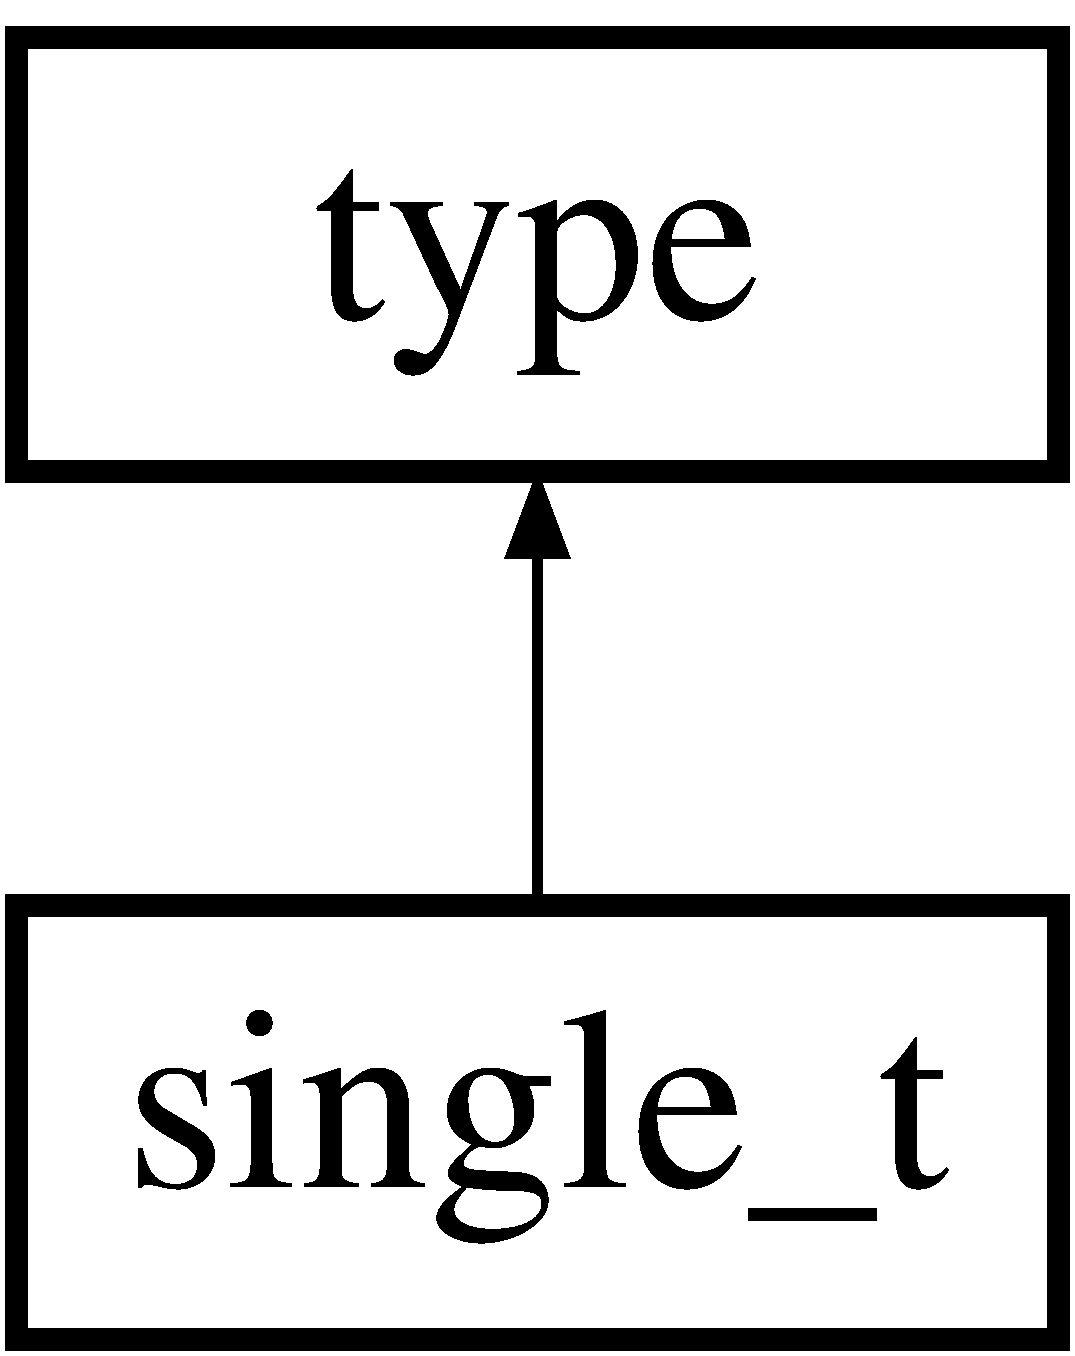
\includegraphics[height=2.000000cm]{classsingle__t}
\end{center}
\end{figure}
\subsection*{Public Types}
\begin{DoxyCompactItemize}
\item 
typedef \+::\hyperlink{classvector__t}{vector\+\_\+t} \hyperlink{classsingle__t_a07d764e683fbb0e8ddd97945f2c01270}{coord\+\_\+type}
\item 
typedef \+::xsd\+::cxx\+::tree\+::traits$<$ \hyperlink{classsingle__t_a07d764e683fbb0e8ddd97945f2c01270}{coord\+\_\+type}, char $>$ \hyperlink{classsingle__t_aaf92d8da07f04ceb7cc4dbb9a750fb41}{coord\+\_\+traits}
\item 
typedef \+::\hyperlink{classvector__t}{vector\+\_\+t} \hyperlink{classsingle__t_a1ed86c81a135e0a683e85f53b882817e}{force\+\_\+type}
\item 
typedef \+::xsd\+::cxx\+::tree\+::optional$<$ \hyperlink{classsingle__t_a1ed86c81a135e0a683e85f53b882817e}{force\+\_\+type} $>$ \hyperlink{classsingle__t_a33128be3fe89ddbab885d0a205d35888}{force\+\_\+optional}
\item 
typedef \+::xsd\+::cxx\+::tree\+::traits$<$ \hyperlink{classsingle__t_a1ed86c81a135e0a683e85f53b882817e}{force\+\_\+type}, char $>$ \hyperlink{classsingle__t_aeccb5e0ed757624999b2bb071e656aaa}{force\+\_\+traits}
\item 
typedef \+::\hyperlink{classvector__t}{vector\+\_\+t} \hyperlink{classsingle__t_a5aa793b7c32fb659668bbac250ce7d6b}{velocity\+\_\+type}
\item 
typedef \+::xsd\+::cxx\+::tree\+::traits$<$ \hyperlink{classsingle__t_a5aa793b7c32fb659668bbac250ce7d6b}{velocity\+\_\+type}, char $>$ \hyperlink{classsingle__t_ad427fe4b91c2b35163cd993438aba00a}{velocity\+\_\+traits}
\item 
typedef \+::\hyperlink{namespacexml__schema_acfa24ac68e1a188e7f44c36f7a158bf4}{xml\+\_\+schema\+::int\+\_\+} \hyperlink{classsingle__t_a6ae5872727b5902a3907ef699bcc5ee0}{type\+\_\+type}
\item 
typedef \+::xsd\+::cxx\+::tree\+::traits$<$ \hyperlink{classsingle__t_a6ae5872727b5902a3907ef699bcc5ee0}{type\+\_\+type}, char $>$ \hyperlink{classsingle__t_a5c4f2eba1499ec313d4236b4e6fb8eea}{type\+\_\+traits}
\end{DoxyCompactItemize}
\subsection*{Public Member Functions}
\begin{DoxyCompactItemize}
\item 
const \hyperlink{classsingle__t_a07d764e683fbb0e8ddd97945f2c01270}{coord\+\_\+type} \& \hyperlink{classsingle__t_a385ac1cabe51a4a6c3bded8e27d94906}{coord} () const 
\item 
\hyperlink{classsingle__t_a07d764e683fbb0e8ddd97945f2c01270}{coord\+\_\+type} \& \hyperlink{classsingle__t_a3d561a81560c220d19f20b890668464d}{coord} ()
\item 
void \hyperlink{classsingle__t_a9d2bd91b3955fcd17fc0a50dcce479a0}{coord} (const \hyperlink{classsingle__t_a07d764e683fbb0e8ddd97945f2c01270}{coord\+\_\+type} \&x)
\item 
void \hyperlink{classsingle__t_aa477c688525dc47de3b401555e80e091}{coord} (\+::std\+::unique\+\_\+ptr$<$ \hyperlink{classsingle__t_a07d764e683fbb0e8ddd97945f2c01270}{coord\+\_\+type} $>$ p)
\item 
const \hyperlink{classsingle__t_a33128be3fe89ddbab885d0a205d35888}{force\+\_\+optional} \& \hyperlink{classsingle__t_a9dd5318bc78873ff6cd71e92b95d8f39}{force} () const 
\item 
\hyperlink{classsingle__t_a33128be3fe89ddbab885d0a205d35888}{force\+\_\+optional} \& \hyperlink{classsingle__t_a4a729c76cbf95d42bebc965526dfc739}{force} ()
\item 
void \hyperlink{classsingle__t_afbfa0efe703c817e1eda807360c577e4}{force} (const \hyperlink{classsingle__t_a1ed86c81a135e0a683e85f53b882817e}{force\+\_\+type} \&x)
\item 
void \hyperlink{classsingle__t_ad492464958bfebb60964334dd49a8c98}{force} (const \hyperlink{classsingle__t_a33128be3fe89ddbab885d0a205d35888}{force\+\_\+optional} \&x)
\item 
void \hyperlink{classsingle__t_ab548ea6047d7b5c100a441e09c79b20e}{force} (\+::std\+::unique\+\_\+ptr$<$ \hyperlink{classsingle__t_a1ed86c81a135e0a683e85f53b882817e}{force\+\_\+type} $>$ p)
\item 
const \hyperlink{classsingle__t_a5aa793b7c32fb659668bbac250ce7d6b}{velocity\+\_\+type} \& \hyperlink{classsingle__t_a865209c855bc4b3e0bfa22820af0602a}{velocity} () const 
\item 
\hyperlink{classsingle__t_a5aa793b7c32fb659668bbac250ce7d6b}{velocity\+\_\+type} \& \hyperlink{classsingle__t_a315489c251504a68a58c9b7ab00a5b39}{velocity} ()
\item 
void \hyperlink{classsingle__t_a3f97cd5cab3b100483d1a98ee95379fe}{velocity} (const \hyperlink{classsingle__t_a5aa793b7c32fb659668bbac250ce7d6b}{velocity\+\_\+type} \&x)
\item 
void \hyperlink{classsingle__t_a774ab1e29d33b94a6fb64a078b921414}{velocity} (\+::std\+::unique\+\_\+ptr$<$ \hyperlink{classsingle__t_a5aa793b7c32fb659668bbac250ce7d6b}{velocity\+\_\+type} $>$ p)
\item 
const \hyperlink{classsingle__t_a6ae5872727b5902a3907ef699bcc5ee0}{type\+\_\+type} \& \hyperlink{classsingle__t_a71ecdc5b5e9912a5f36a0efb4210f336}{type} () const 
\item 
\hyperlink{classsingle__t_a6ae5872727b5902a3907ef699bcc5ee0}{type\+\_\+type} \& \hyperlink{classsingle__t_adda2ad1ff7b84e24fe32bf2865ae9412}{type} ()
\item 
void \hyperlink{classsingle__t_a8e8b52c6863fc6777b03e2782fd23594}{type} (const \hyperlink{classsingle__t_a6ae5872727b5902a3907ef699bcc5ee0}{type\+\_\+type} \&x)
\item 
\hyperlink{classsingle__t_a95f4b77b3f49a5363d84e713c5c74f28}{single\+\_\+t} (const \hyperlink{classsingle__t_a07d764e683fbb0e8ddd97945f2c01270}{coord\+\_\+type} \&, const \hyperlink{classsingle__t_a5aa793b7c32fb659668bbac250ce7d6b}{velocity\+\_\+type} \&, const \hyperlink{classsingle__t_a6ae5872727b5902a3907ef699bcc5ee0}{type\+\_\+type} \&)
\item 
\hyperlink{classsingle__t_a5bf6773471fc02d9c47bfd4fd7f129f8}{single\+\_\+t} (\+::std\+::unique\+\_\+ptr$<$ \hyperlink{classsingle__t_a07d764e683fbb0e8ddd97945f2c01270}{coord\+\_\+type} $>$,\+::std\+::unique\+\_\+ptr$<$ \hyperlink{classsingle__t_a5aa793b7c32fb659668bbac250ce7d6b}{velocity\+\_\+type} $>$, const \hyperlink{classsingle__t_a6ae5872727b5902a3907ef699bcc5ee0}{type\+\_\+type} \&)
\item 
\hyperlink{classsingle__t_a130764d0ac93705cc451b79f2af2afbd}{single\+\_\+t} (const \+::xercesc\+::\+D\+O\+M\+Element \&e,\+::\hyperlink{namespacexml__schema_a0612287d030cb2732d31a45b258fdc87}{xml\+\_\+schema\+::flags} f=0,\+::\hyperlink{namespacexml__schema_ada9aa30dc722e93ee2ed7243085402a5}{xml\+\_\+schema\+::container} $\ast$c=0)
\item 
\hyperlink{classsingle__t_a94974f20fe6b61bf7c9c9466f7a6c472}{single\+\_\+t} (const \hyperlink{classsingle__t}{single\+\_\+t} \&x,\+::\hyperlink{namespacexml__schema_a0612287d030cb2732d31a45b258fdc87}{xml\+\_\+schema\+::flags} f=0,\+::\hyperlink{namespacexml__schema_ada9aa30dc722e93ee2ed7243085402a5}{xml\+\_\+schema\+::container} $\ast$c=0)
\item 
virtual \hyperlink{classsingle__t}{single\+\_\+t} $\ast$ \hyperlink{classsingle__t_abe99b1388d184b22b23f5e42cb046945}{\+\_\+clone} (\+::\hyperlink{namespacexml__schema_a0612287d030cb2732d31a45b258fdc87}{xml\+\_\+schema\+::flags} f=0,\+::\hyperlink{namespacexml__schema_ada9aa30dc722e93ee2ed7243085402a5}{xml\+\_\+schema\+::container} $\ast$c=0) const 
\item 
\hyperlink{classsingle__t}{single\+\_\+t} \& \hyperlink{classsingle__t_a1b34e3eb88ee12e34caa75518e6f03eb}{operator=} (const \hyperlink{classsingle__t}{single\+\_\+t} \&x)
\item 
virtual \hyperlink{classsingle__t_a4771d9de9082d49504b2836193853042}{$\sim$single\+\_\+t} ()
\end{DoxyCompactItemize}
\subsection*{Protected Member Functions}
\begin{DoxyCompactItemize}
\item 
void \hyperlink{classsingle__t_a24857efb767f94282d199e281d197c3a}{parse} (\+::xsd\+::cxx\+::xml\+::dom\+::parser$<$ char $>$ \&,\+::\hyperlink{namespacexml__schema_a0612287d030cb2732d31a45b258fdc87}{xml\+\_\+schema\+::flags})
\end{DoxyCompactItemize}
\subsection*{Protected Attributes}
\begin{DoxyCompactItemize}
\item 
\+::xsd\+::cxx\+::tree\+::one$<$ \hyperlink{classsingle__t_a07d764e683fbb0e8ddd97945f2c01270}{coord\+\_\+type} $>$ \hyperlink{classsingle__t_a88c8130f542d90b17800fe59ed9aabed}{coord\+\_\+}
\item 
\hyperlink{classsingle__t_a33128be3fe89ddbab885d0a205d35888}{force\+\_\+optional} \hyperlink{classsingle__t_a1e9b2a89d19cfdd6842b3611c8dac6cc}{force\+\_\+}
\item 
\+::xsd\+::cxx\+::tree\+::one$<$ \hyperlink{classsingle__t_a5aa793b7c32fb659668bbac250ce7d6b}{velocity\+\_\+type} $>$ \hyperlink{classsingle__t_ae84160509acab4c517aa11c096dd54dd}{velocity\+\_\+}
\item 
\+::xsd\+::cxx\+::tree\+::one$<$ \hyperlink{classsingle__t_a6ae5872727b5902a3907ef699bcc5ee0}{type\+\_\+type} $>$ \hyperlink{classsingle__t_a4df4719166dbbf3b754b192f386aa974}{type\+\_\+}
\end{DoxyCompactItemize}


\subsection{Member Typedef Documentation}
\index{single\+\_\+t@{single\+\_\+t}!coord\+\_\+traits@{coord\+\_\+traits}}
\index{coord\+\_\+traits@{coord\+\_\+traits}!single\+\_\+t@{single\+\_\+t}}
\subsubsection[{\texorpdfstring{coord\+\_\+traits}{coord_traits}}]{\setlength{\rightskip}{0pt plus 5cm}typedef \+::xsd\+::cxx\+::tree\+::traits$<$ {\bf coord\+\_\+type}, char $>$ {\bf single\+\_\+t\+::coord\+\_\+traits}}\hypertarget{classsingle__t_aaf92d8da07f04ceb7cc4dbb9a750fb41}{}\label{classsingle__t_aaf92d8da07f04ceb7cc4dbb9a750fb41}
\index{single\+\_\+t@{single\+\_\+t}!coord\+\_\+type@{coord\+\_\+type}}
\index{coord\+\_\+type@{coord\+\_\+type}!single\+\_\+t@{single\+\_\+t}}
\subsubsection[{\texorpdfstring{coord\+\_\+type}{coord_type}}]{\setlength{\rightskip}{0pt plus 5cm}typedef \+::{\bf vector\+\_\+t} {\bf single\+\_\+t\+::coord\+\_\+type}}\hypertarget{classsingle__t_a07d764e683fbb0e8ddd97945f2c01270}{}\label{classsingle__t_a07d764e683fbb0e8ddd97945f2c01270}
\index{single\+\_\+t@{single\+\_\+t}!force\+\_\+optional@{force\+\_\+optional}}
\index{force\+\_\+optional@{force\+\_\+optional}!single\+\_\+t@{single\+\_\+t}}
\subsubsection[{\texorpdfstring{force\+\_\+optional}{force_optional}}]{\setlength{\rightskip}{0pt plus 5cm}typedef \+::xsd\+::cxx\+::tree\+::optional$<$ {\bf force\+\_\+type} $>$ {\bf single\+\_\+t\+::force\+\_\+optional}}\hypertarget{classsingle__t_a33128be3fe89ddbab885d0a205d35888}{}\label{classsingle__t_a33128be3fe89ddbab885d0a205d35888}
\index{single\+\_\+t@{single\+\_\+t}!force\+\_\+traits@{force\+\_\+traits}}
\index{force\+\_\+traits@{force\+\_\+traits}!single\+\_\+t@{single\+\_\+t}}
\subsubsection[{\texorpdfstring{force\+\_\+traits}{force_traits}}]{\setlength{\rightskip}{0pt plus 5cm}typedef \+::xsd\+::cxx\+::tree\+::traits$<$ {\bf force\+\_\+type}, char $>$ {\bf single\+\_\+t\+::force\+\_\+traits}}\hypertarget{classsingle__t_aeccb5e0ed757624999b2bb071e656aaa}{}\label{classsingle__t_aeccb5e0ed757624999b2bb071e656aaa}
\index{single\+\_\+t@{single\+\_\+t}!force\+\_\+type@{force\+\_\+type}}
\index{force\+\_\+type@{force\+\_\+type}!single\+\_\+t@{single\+\_\+t}}
\subsubsection[{\texorpdfstring{force\+\_\+type}{force_type}}]{\setlength{\rightskip}{0pt plus 5cm}typedef \+::{\bf vector\+\_\+t} {\bf single\+\_\+t\+::force\+\_\+type}}\hypertarget{classsingle__t_a1ed86c81a135e0a683e85f53b882817e}{}\label{classsingle__t_a1ed86c81a135e0a683e85f53b882817e}
\index{single\+\_\+t@{single\+\_\+t}!type\+\_\+traits@{type\+\_\+traits}}
\index{type\+\_\+traits@{type\+\_\+traits}!single\+\_\+t@{single\+\_\+t}}
\subsubsection[{\texorpdfstring{type\+\_\+traits}{type_traits}}]{\setlength{\rightskip}{0pt plus 5cm}typedef \+::xsd\+::cxx\+::tree\+::traits$<$ {\bf type\+\_\+type}, char $>$ {\bf single\+\_\+t\+::type\+\_\+traits}}\hypertarget{classsingle__t_a5c4f2eba1499ec313d4236b4e6fb8eea}{}\label{classsingle__t_a5c4f2eba1499ec313d4236b4e6fb8eea}
\index{single\+\_\+t@{single\+\_\+t}!type\+\_\+type@{type\+\_\+type}}
\index{type\+\_\+type@{type\+\_\+type}!single\+\_\+t@{single\+\_\+t}}
\subsubsection[{\texorpdfstring{type\+\_\+type}{type_type}}]{\setlength{\rightskip}{0pt plus 5cm}typedef \+::{\bf xml\+\_\+schema\+::int\+\_\+} {\bf single\+\_\+t\+::type\+\_\+type}}\hypertarget{classsingle__t_a6ae5872727b5902a3907ef699bcc5ee0}{}\label{classsingle__t_a6ae5872727b5902a3907ef699bcc5ee0}
\index{single\+\_\+t@{single\+\_\+t}!velocity\+\_\+traits@{velocity\+\_\+traits}}
\index{velocity\+\_\+traits@{velocity\+\_\+traits}!single\+\_\+t@{single\+\_\+t}}
\subsubsection[{\texorpdfstring{velocity\+\_\+traits}{velocity_traits}}]{\setlength{\rightskip}{0pt plus 5cm}typedef \+::xsd\+::cxx\+::tree\+::traits$<$ {\bf velocity\+\_\+type}, char $>$ {\bf single\+\_\+t\+::velocity\+\_\+traits}}\hypertarget{classsingle__t_ad427fe4b91c2b35163cd993438aba00a}{}\label{classsingle__t_ad427fe4b91c2b35163cd993438aba00a}
\index{single\+\_\+t@{single\+\_\+t}!velocity\+\_\+type@{velocity\+\_\+type}}
\index{velocity\+\_\+type@{velocity\+\_\+type}!single\+\_\+t@{single\+\_\+t}}
\subsubsection[{\texorpdfstring{velocity\+\_\+type}{velocity_type}}]{\setlength{\rightskip}{0pt plus 5cm}typedef \+::{\bf vector\+\_\+t} {\bf single\+\_\+t\+::velocity\+\_\+type}}\hypertarget{classsingle__t_a5aa793b7c32fb659668bbac250ce7d6b}{}\label{classsingle__t_a5aa793b7c32fb659668bbac250ce7d6b}


\subsection{Constructor \& Destructor Documentation}
\index{single\+\_\+t@{single\+\_\+t}!single\+\_\+t@{single\+\_\+t}}
\index{single\+\_\+t@{single\+\_\+t}!single\+\_\+t@{single\+\_\+t}}
\subsubsection[{\texorpdfstring{single\+\_\+t(const coord\+\_\+type \&, const velocity\+\_\+type \&, const type\+\_\+type \&)}{single_t(const coord_type &, const velocity_type &, const type_type &)}}]{\setlength{\rightskip}{0pt plus 5cm}single\+\_\+t\+::single\+\_\+t (
\begin{DoxyParamCaption}
\item[{const {\bf coord\+\_\+type} \&}]{coord, }
\item[{const {\bf velocity\+\_\+type} \&}]{velocity, }
\item[{const {\bf type\+\_\+type} \&}]{type}
\end{DoxyParamCaption}
)}\hypertarget{classsingle__t_a95f4b77b3f49a5363d84e713c5c74f28}{}\label{classsingle__t_a95f4b77b3f49a5363d84e713c5c74f28}
\index{single\+\_\+t@{single\+\_\+t}!single\+\_\+t@{single\+\_\+t}}
\index{single\+\_\+t@{single\+\_\+t}!single\+\_\+t@{single\+\_\+t}}
\subsubsection[{\texorpdfstring{single\+\_\+t(\+::std\+::unique\+\_\+ptr$<$ coord\+\_\+type $>$,\+::std\+::unique\+\_\+ptr$<$ velocity\+\_\+type $>$, const type\+\_\+type \&)}{single_t(::std::unique_ptr< coord_type >,::std::unique_ptr< velocity_type >, const type_type &)}}]{\setlength{\rightskip}{0pt plus 5cm}single\+\_\+t\+::single\+\_\+t (
\begin{DoxyParamCaption}
\item[{\+::std\+::unique\+\_\+ptr$<$ {\bf coord\+\_\+type} $>$}]{coord, }
\item[{\+::std\+::unique\+\_\+ptr$<$ {\bf velocity\+\_\+type} $>$}]{velocity, }
\item[{const {\bf type\+\_\+type} \&}]{type}
\end{DoxyParamCaption}
)}\hypertarget{classsingle__t_a5bf6773471fc02d9c47bfd4fd7f129f8}{}\label{classsingle__t_a5bf6773471fc02d9c47bfd4fd7f129f8}
\index{single\+\_\+t@{single\+\_\+t}!single\+\_\+t@{single\+\_\+t}}
\index{single\+\_\+t@{single\+\_\+t}!single\+\_\+t@{single\+\_\+t}}
\subsubsection[{\texorpdfstring{single\+\_\+t(const \+::xercesc\+::\+D\+O\+M\+Element \&e,\+::xml\+\_\+schema\+::flags f=0,\+::xml\+\_\+schema\+::container $\ast$c=0)}{single_t(const ::xercesc::DOMElement &e,::xml_schema::flags f=0,::xml_schema::container *c=0)}}]{\setlength{\rightskip}{0pt plus 5cm}single\+\_\+t\+::single\+\_\+t (
\begin{DoxyParamCaption}
\item[{const \+::xercesc\+::\+D\+O\+M\+Element \&}]{e, }
\item[{\+::{\bf xml\+\_\+schema\+::flags}}]{f = {\ttfamily 0}, }
\item[{\+::{\bf xml\+\_\+schema\+::container} $\ast$}]{c = {\ttfamily 0}}
\end{DoxyParamCaption}
)}\hypertarget{classsingle__t_a130764d0ac93705cc451b79f2af2afbd}{}\label{classsingle__t_a130764d0ac93705cc451b79f2af2afbd}
\index{single\+\_\+t@{single\+\_\+t}!single\+\_\+t@{single\+\_\+t}}
\index{single\+\_\+t@{single\+\_\+t}!single\+\_\+t@{single\+\_\+t}}
\subsubsection[{\texorpdfstring{single\+\_\+t(const single\+\_\+t \&x,\+::xml\+\_\+schema\+::flags f=0,\+::xml\+\_\+schema\+::container $\ast$c=0)}{single_t(const single_t &x,::xml_schema::flags f=0,::xml_schema::container *c=0)}}]{\setlength{\rightskip}{0pt plus 5cm}single\+\_\+t\+::single\+\_\+t (
\begin{DoxyParamCaption}
\item[{const {\bf single\+\_\+t} \&}]{x, }
\item[{\+::{\bf xml\+\_\+schema\+::flags}}]{f = {\ttfamily 0}, }
\item[{\+::{\bf xml\+\_\+schema\+::container} $\ast$}]{c = {\ttfamily 0}}
\end{DoxyParamCaption}
)}\hypertarget{classsingle__t_a94974f20fe6b61bf7c9c9466f7a6c472}{}\label{classsingle__t_a94974f20fe6b61bf7c9c9466f7a6c472}
\index{single\+\_\+t@{single\+\_\+t}!````~single\+\_\+t@{$\sim$single\+\_\+t}}
\index{````~single\+\_\+t@{$\sim$single\+\_\+t}!single\+\_\+t@{single\+\_\+t}}
\subsubsection[{\texorpdfstring{$\sim$single\+\_\+t()}{~single_t()}}]{\setlength{\rightskip}{0pt plus 5cm}single\+\_\+t\+::$\sim$single\+\_\+t (
\begin{DoxyParamCaption}
{}
\end{DoxyParamCaption}
)\hspace{0.3cm}{\ttfamily [virtual]}}\hypertarget{classsingle__t_a4771d9de9082d49504b2836193853042}{}\label{classsingle__t_a4771d9de9082d49504b2836193853042}


\subsection{Member Function Documentation}
\index{single\+\_\+t@{single\+\_\+t}!\+\_\+clone@{\+\_\+clone}}
\index{\+\_\+clone@{\+\_\+clone}!single\+\_\+t@{single\+\_\+t}}
\subsubsection[{\texorpdfstring{\+\_\+clone(\+::xml\+\_\+schema\+::flags f=0,\+::xml\+\_\+schema\+::container $\ast$c=0) const }{_clone(::xml_schema::flags f=0,::xml_schema::container *c=0) const }}]{\setlength{\rightskip}{0pt plus 5cm}{\bf single\+\_\+t} $\ast$ single\+\_\+t\+::\+\_\+clone (
\begin{DoxyParamCaption}
\item[{\+::{\bf xml\+\_\+schema\+::flags}}]{f = {\ttfamily 0}, }
\item[{\+::{\bf xml\+\_\+schema\+::container} $\ast$}]{c = {\ttfamily 0}}
\end{DoxyParamCaption}
) const\hspace{0.3cm}{\ttfamily [virtual]}}\hypertarget{classsingle__t_abe99b1388d184b22b23f5e42cb046945}{}\label{classsingle__t_abe99b1388d184b22b23f5e42cb046945}
\index{single\+\_\+t@{single\+\_\+t}!coord@{coord}}
\index{coord@{coord}!single\+\_\+t@{single\+\_\+t}}
\subsubsection[{\texorpdfstring{coord() const }{coord() const }}]{\setlength{\rightskip}{0pt plus 5cm}const {\bf single\+\_\+t\+::coord\+\_\+type} \& single\+\_\+t\+::coord (
\begin{DoxyParamCaption}
{}
\end{DoxyParamCaption}
) const}\hypertarget{classsingle__t_a385ac1cabe51a4a6c3bded8e27d94906}{}\label{classsingle__t_a385ac1cabe51a4a6c3bded8e27d94906}
\index{single\+\_\+t@{single\+\_\+t}!coord@{coord}}
\index{coord@{coord}!single\+\_\+t@{single\+\_\+t}}
\subsubsection[{\texorpdfstring{coord()}{coord()}}]{\setlength{\rightskip}{0pt plus 5cm}{\bf single\+\_\+t\+::coord\+\_\+type} \& single\+\_\+t\+::coord (
\begin{DoxyParamCaption}
{}
\end{DoxyParamCaption}
)}\hypertarget{classsingle__t_a3d561a81560c220d19f20b890668464d}{}\label{classsingle__t_a3d561a81560c220d19f20b890668464d}
\index{single\+\_\+t@{single\+\_\+t}!coord@{coord}}
\index{coord@{coord}!single\+\_\+t@{single\+\_\+t}}
\subsubsection[{\texorpdfstring{coord(const coord\+\_\+type \&x)}{coord(const coord_type &x)}}]{\setlength{\rightskip}{0pt plus 5cm}void single\+\_\+t\+::coord (
\begin{DoxyParamCaption}
\item[{const {\bf coord\+\_\+type} \&}]{x}
\end{DoxyParamCaption}
)}\hypertarget{classsingle__t_a9d2bd91b3955fcd17fc0a50dcce479a0}{}\label{classsingle__t_a9d2bd91b3955fcd17fc0a50dcce479a0}
\index{single\+\_\+t@{single\+\_\+t}!coord@{coord}}
\index{coord@{coord}!single\+\_\+t@{single\+\_\+t}}
\subsubsection[{\texorpdfstring{coord(\+::std\+::unique\+\_\+ptr$<$ coord\+\_\+type $>$ p)}{coord(::std::unique_ptr< coord_type > p)}}]{\setlength{\rightskip}{0pt plus 5cm}void single\+\_\+t\+::coord (
\begin{DoxyParamCaption}
\item[{\+::std\+::unique\+\_\+ptr$<$ {\bf coord\+\_\+type} $>$}]{p}
\end{DoxyParamCaption}
)}\hypertarget{classsingle__t_aa477c688525dc47de3b401555e80e091}{}\label{classsingle__t_aa477c688525dc47de3b401555e80e091}
\index{single\+\_\+t@{single\+\_\+t}!force@{force}}
\index{force@{force}!single\+\_\+t@{single\+\_\+t}}
\subsubsection[{\texorpdfstring{force() const }{force() const }}]{\setlength{\rightskip}{0pt plus 5cm}const {\bf single\+\_\+t\+::force\+\_\+optional} \& single\+\_\+t\+::force (
\begin{DoxyParamCaption}
{}
\end{DoxyParamCaption}
) const}\hypertarget{classsingle__t_a9dd5318bc78873ff6cd71e92b95d8f39}{}\label{classsingle__t_a9dd5318bc78873ff6cd71e92b95d8f39}
\index{single\+\_\+t@{single\+\_\+t}!force@{force}}
\index{force@{force}!single\+\_\+t@{single\+\_\+t}}
\subsubsection[{\texorpdfstring{force()}{force()}}]{\setlength{\rightskip}{0pt plus 5cm}{\bf single\+\_\+t\+::force\+\_\+optional} \& single\+\_\+t\+::force (
\begin{DoxyParamCaption}
{}
\end{DoxyParamCaption}
)}\hypertarget{classsingle__t_a4a729c76cbf95d42bebc965526dfc739}{}\label{classsingle__t_a4a729c76cbf95d42bebc965526dfc739}
\index{single\+\_\+t@{single\+\_\+t}!force@{force}}
\index{force@{force}!single\+\_\+t@{single\+\_\+t}}
\subsubsection[{\texorpdfstring{force(const force\+\_\+type \&x)}{force(const force_type &x)}}]{\setlength{\rightskip}{0pt plus 5cm}void single\+\_\+t\+::force (
\begin{DoxyParamCaption}
\item[{const {\bf force\+\_\+type} \&}]{x}
\end{DoxyParamCaption}
)}\hypertarget{classsingle__t_afbfa0efe703c817e1eda807360c577e4}{}\label{classsingle__t_afbfa0efe703c817e1eda807360c577e4}
\index{single\+\_\+t@{single\+\_\+t}!force@{force}}
\index{force@{force}!single\+\_\+t@{single\+\_\+t}}
\subsubsection[{\texorpdfstring{force(const force\+\_\+optional \&x)}{force(const force_optional &x)}}]{\setlength{\rightskip}{0pt plus 5cm}void single\+\_\+t\+::force (
\begin{DoxyParamCaption}
\item[{const {\bf force\+\_\+optional} \&}]{x}
\end{DoxyParamCaption}
)}\hypertarget{classsingle__t_ad492464958bfebb60964334dd49a8c98}{}\label{classsingle__t_ad492464958bfebb60964334dd49a8c98}
\index{single\+\_\+t@{single\+\_\+t}!force@{force}}
\index{force@{force}!single\+\_\+t@{single\+\_\+t}}
\subsubsection[{\texorpdfstring{force(\+::std\+::unique\+\_\+ptr$<$ force\+\_\+type $>$ p)}{force(::std::unique_ptr< force_type > p)}}]{\setlength{\rightskip}{0pt plus 5cm}void single\+\_\+t\+::force (
\begin{DoxyParamCaption}
\item[{\+::std\+::unique\+\_\+ptr$<$ {\bf force\+\_\+type} $>$}]{p}
\end{DoxyParamCaption}
)}\hypertarget{classsingle__t_ab548ea6047d7b5c100a441e09c79b20e}{}\label{classsingle__t_ab548ea6047d7b5c100a441e09c79b20e}
\index{single\+\_\+t@{single\+\_\+t}!operator=@{operator=}}
\index{operator=@{operator=}!single\+\_\+t@{single\+\_\+t}}
\subsubsection[{\texorpdfstring{operator=(const single\+\_\+t \&x)}{operator=(const single_t &x)}}]{\setlength{\rightskip}{0pt plus 5cm}{\bf single\+\_\+t} \& single\+\_\+t\+::operator= (
\begin{DoxyParamCaption}
\item[{const {\bf single\+\_\+t} \&}]{x}
\end{DoxyParamCaption}
)}\hypertarget{classsingle__t_a1b34e3eb88ee12e34caa75518e6f03eb}{}\label{classsingle__t_a1b34e3eb88ee12e34caa75518e6f03eb}
\index{single\+\_\+t@{single\+\_\+t}!parse@{parse}}
\index{parse@{parse}!single\+\_\+t@{single\+\_\+t}}
\subsubsection[{\texorpdfstring{parse(\+::xsd\+::cxx\+::xml\+::dom\+::parser$<$ char $>$ \&,\+::xml\+\_\+schema\+::flags)}{parse(::xsd::cxx::xml::dom::parser< char > &,::xml_schema::flags)}}]{\setlength{\rightskip}{0pt plus 5cm}void single\+\_\+t\+::parse (
\begin{DoxyParamCaption}
\item[{\+::xsd\+::cxx\+::xml\+::dom\+::parser$<$ char $>$ \&}]{p, }
\item[{\+::{\bf xml\+\_\+schema\+::flags}}]{f}
\end{DoxyParamCaption}
)\hspace{0.3cm}{\ttfamily [protected]}}\hypertarget{classsingle__t_a24857efb767f94282d199e281d197c3a}{}\label{classsingle__t_a24857efb767f94282d199e281d197c3a}
\index{single\+\_\+t@{single\+\_\+t}!type@{type}}
\index{type@{type}!single\+\_\+t@{single\+\_\+t}}
\subsubsection[{\texorpdfstring{type() const }{type() const }}]{\setlength{\rightskip}{0pt plus 5cm}const {\bf single\+\_\+t\+::type\+\_\+type} \& single\+\_\+t\+::type (
\begin{DoxyParamCaption}
{}
\end{DoxyParamCaption}
) const}\hypertarget{classsingle__t_a71ecdc5b5e9912a5f36a0efb4210f336}{}\label{classsingle__t_a71ecdc5b5e9912a5f36a0efb4210f336}
\index{single\+\_\+t@{single\+\_\+t}!type@{type}}
\index{type@{type}!single\+\_\+t@{single\+\_\+t}}
\subsubsection[{\texorpdfstring{type()}{type()}}]{\setlength{\rightskip}{0pt plus 5cm}{\bf single\+\_\+t\+::type\+\_\+type} \& single\+\_\+t\+::type (
\begin{DoxyParamCaption}
{}
\end{DoxyParamCaption}
)}\hypertarget{classsingle__t_adda2ad1ff7b84e24fe32bf2865ae9412}{}\label{classsingle__t_adda2ad1ff7b84e24fe32bf2865ae9412}
\index{single\+\_\+t@{single\+\_\+t}!type@{type}}
\index{type@{type}!single\+\_\+t@{single\+\_\+t}}
\subsubsection[{\texorpdfstring{type(const type\+\_\+type \&x)}{type(const type_type &x)}}]{\setlength{\rightskip}{0pt plus 5cm}void single\+\_\+t\+::type (
\begin{DoxyParamCaption}
\item[{const {\bf type\+\_\+type} \&}]{x}
\end{DoxyParamCaption}
)}\hypertarget{classsingle__t_a8e8b52c6863fc6777b03e2782fd23594}{}\label{classsingle__t_a8e8b52c6863fc6777b03e2782fd23594}
\index{single\+\_\+t@{single\+\_\+t}!velocity@{velocity}}
\index{velocity@{velocity}!single\+\_\+t@{single\+\_\+t}}
\subsubsection[{\texorpdfstring{velocity() const }{velocity() const }}]{\setlength{\rightskip}{0pt plus 5cm}const {\bf single\+\_\+t\+::velocity\+\_\+type} \& single\+\_\+t\+::velocity (
\begin{DoxyParamCaption}
{}
\end{DoxyParamCaption}
) const}\hypertarget{classsingle__t_a865209c855bc4b3e0bfa22820af0602a}{}\label{classsingle__t_a865209c855bc4b3e0bfa22820af0602a}
\index{single\+\_\+t@{single\+\_\+t}!velocity@{velocity}}
\index{velocity@{velocity}!single\+\_\+t@{single\+\_\+t}}
\subsubsection[{\texorpdfstring{velocity()}{velocity()}}]{\setlength{\rightskip}{0pt plus 5cm}{\bf single\+\_\+t\+::velocity\+\_\+type} \& single\+\_\+t\+::velocity (
\begin{DoxyParamCaption}
{}
\end{DoxyParamCaption}
)}\hypertarget{classsingle__t_a315489c251504a68a58c9b7ab00a5b39}{}\label{classsingle__t_a315489c251504a68a58c9b7ab00a5b39}
\index{single\+\_\+t@{single\+\_\+t}!velocity@{velocity}}
\index{velocity@{velocity}!single\+\_\+t@{single\+\_\+t}}
\subsubsection[{\texorpdfstring{velocity(const velocity\+\_\+type \&x)}{velocity(const velocity_type &x)}}]{\setlength{\rightskip}{0pt plus 5cm}void single\+\_\+t\+::velocity (
\begin{DoxyParamCaption}
\item[{const {\bf velocity\+\_\+type} \&}]{x}
\end{DoxyParamCaption}
)}\hypertarget{classsingle__t_a3f97cd5cab3b100483d1a98ee95379fe}{}\label{classsingle__t_a3f97cd5cab3b100483d1a98ee95379fe}
\index{single\+\_\+t@{single\+\_\+t}!velocity@{velocity}}
\index{velocity@{velocity}!single\+\_\+t@{single\+\_\+t}}
\subsubsection[{\texorpdfstring{velocity(\+::std\+::unique\+\_\+ptr$<$ velocity\+\_\+type $>$ p)}{velocity(::std::unique_ptr< velocity_type > p)}}]{\setlength{\rightskip}{0pt plus 5cm}void single\+\_\+t\+::velocity (
\begin{DoxyParamCaption}
\item[{\+::std\+::unique\+\_\+ptr$<$ {\bf velocity\+\_\+type} $>$}]{p}
\end{DoxyParamCaption}
)}\hypertarget{classsingle__t_a774ab1e29d33b94a6fb64a078b921414}{}\label{classsingle__t_a774ab1e29d33b94a6fb64a078b921414}


\subsection{Member Data Documentation}
\index{single\+\_\+t@{single\+\_\+t}!coord\+\_\+@{coord\+\_\+}}
\index{coord\+\_\+@{coord\+\_\+}!single\+\_\+t@{single\+\_\+t}}
\subsubsection[{\texorpdfstring{coord\+\_\+}{coord_}}]{\setlength{\rightskip}{0pt plus 5cm}\+::xsd\+::cxx\+::tree\+::one$<$ {\bf coord\+\_\+type} $>$ single\+\_\+t\+::coord\+\_\+\hspace{0.3cm}{\ttfamily [protected]}}\hypertarget{classsingle__t_a88c8130f542d90b17800fe59ed9aabed}{}\label{classsingle__t_a88c8130f542d90b17800fe59ed9aabed}
\index{single\+\_\+t@{single\+\_\+t}!force\+\_\+@{force\+\_\+}}
\index{force\+\_\+@{force\+\_\+}!single\+\_\+t@{single\+\_\+t}}
\subsubsection[{\texorpdfstring{force\+\_\+}{force_}}]{\setlength{\rightskip}{0pt plus 5cm}{\bf force\+\_\+optional} single\+\_\+t\+::force\+\_\+\hspace{0.3cm}{\ttfamily [protected]}}\hypertarget{classsingle__t_a1e9b2a89d19cfdd6842b3611c8dac6cc}{}\label{classsingle__t_a1e9b2a89d19cfdd6842b3611c8dac6cc}
\index{single\+\_\+t@{single\+\_\+t}!type\+\_\+@{type\+\_\+}}
\index{type\+\_\+@{type\+\_\+}!single\+\_\+t@{single\+\_\+t}}
\subsubsection[{\texorpdfstring{type\+\_\+}{type_}}]{\setlength{\rightskip}{0pt plus 5cm}\+::xsd\+::cxx\+::tree\+::one$<$ {\bf type\+\_\+type} $>$ single\+\_\+t\+::type\+\_\+\hspace{0.3cm}{\ttfamily [protected]}}\hypertarget{classsingle__t_a4df4719166dbbf3b754b192f386aa974}{}\label{classsingle__t_a4df4719166dbbf3b754b192f386aa974}
\index{single\+\_\+t@{single\+\_\+t}!velocity\+\_\+@{velocity\+\_\+}}
\index{velocity\+\_\+@{velocity\+\_\+}!single\+\_\+t@{single\+\_\+t}}
\subsubsection[{\texorpdfstring{velocity\+\_\+}{velocity_}}]{\setlength{\rightskip}{0pt plus 5cm}\+::xsd\+::cxx\+::tree\+::one$<$ {\bf velocity\+\_\+type} $>$ single\+\_\+t\+::velocity\+\_\+\hspace{0.3cm}{\ttfamily [protected]}}\hypertarget{classsingle__t_ae84160509acab4c517aa11c096dd54dd}{}\label{classsingle__t_ae84160509acab4c517aa11c096dd54dd}


The documentation for this class was generated from the following files\+:\begin{DoxyCompactItemize}
\item 
src/input/\hyperlink{particle__input_8h}{particle\+\_\+input.\+h}\item 
src/input/\hyperlink{particle__input_8cpp}{particle\+\_\+input.\+cpp}\end{DoxyCompactItemize}

\hypertarget{classsphere__t}{}\section{sphere\+\_\+t Class Reference}
\label{classsphere__t}\index{sphere\+\_\+t@{sphere\+\_\+t}}


{\ttfamily \#include $<$particle\+\_\+input.\+h$>$}

Inheritance diagram for sphere\+\_\+t\+:\begin{figure}[H]
\begin{center}
\leavevmode
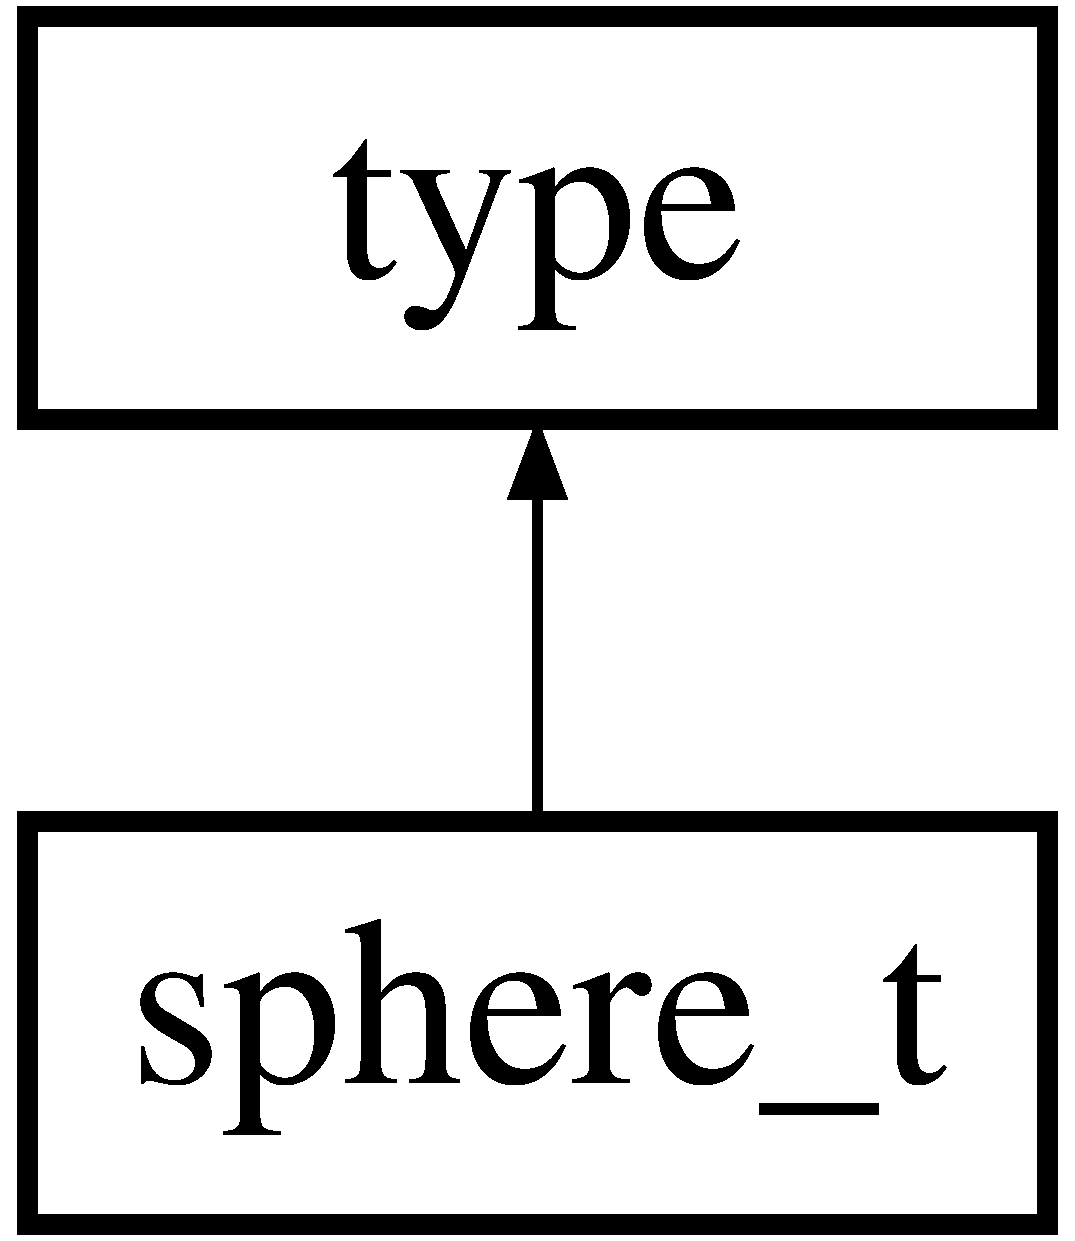
\includegraphics[height=2.000000cm]{classsphere__t}
\end{center}
\end{figure}
\subsection*{Public Types}
\begin{DoxyCompactItemize}
\item 
typedef \+::\hyperlink{classvector__t}{vector\+\_\+t} \hyperlink{classsphere__t_a60b541b054e6695017e6468b51a89efd}{coord\+\_\+type}
\item 
typedef \+::xsd\+::cxx\+::tree\+::traits$<$ \hyperlink{classsphere__t_a60b541b054e6695017e6468b51a89efd}{coord\+\_\+type}, char $>$ \hyperlink{classsphere__t_a87077ccc12086ff4174bcce04de71df7}{coord\+\_\+traits}
\item 
typedef \+::\hyperlink{namespacexml__schema_acfa24ac68e1a188e7f44c36f7a158bf4}{xml\+\_\+schema\+::int\+\_\+} \hyperlink{classsphere__t_a7d5046bdba409d8f49e7c9902ae56278}{radius\+\_\+type}
\item 
typedef \+::xsd\+::cxx\+::tree\+::traits$<$ \hyperlink{classsphere__t_a7d5046bdba409d8f49e7c9902ae56278}{radius\+\_\+type}, char $>$ \hyperlink{classsphere__t_aa2048e5e8155003a2716f8a6e5bd9dea}{radius\+\_\+traits}
\item 
typedef \+::\hyperlink{namespacexml__schema_ad7e04ab17bba0b3fdde43fb79ef6ed87}{xml\+\_\+schema\+::float\+\_\+} \hyperlink{classsphere__t_af7cb7f854954b484b72bbed0516e223a}{mesh\+\_\+type}
\item 
typedef \+::xsd\+::cxx\+::tree\+::traits$<$ \hyperlink{classsphere__t_af7cb7f854954b484b72bbed0516e223a}{mesh\+\_\+type}, char $>$ \hyperlink{classsphere__t_ab459645510e9f8a3a0415beb6d1ce3cd}{mesh\+\_\+traits}
\item 
typedef \+::\hyperlink{classvector__t}{vector\+\_\+t} \hyperlink{classsphere__t_ad38aced876188b1732a5c050670f8cff}{velocity\+\_\+type}
\item 
typedef \+::xsd\+::cxx\+::tree\+::traits$<$ \hyperlink{classsphere__t_ad38aced876188b1732a5c050670f8cff}{velocity\+\_\+type}, char $>$ \hyperlink{classsphere__t_aebe9f6854dfafe65c376fd95c92fd87f}{velocity\+\_\+traits}
\item 
typedef \+::\hyperlink{namespacexml__schema_acfa24ac68e1a188e7f44c36f7a158bf4}{xml\+\_\+schema\+::int\+\_\+} \hyperlink{classsphere__t_a458644a173b4fcac645ccb6e0dd1605f}{type\+\_\+type}
\item 
typedef \+::xsd\+::cxx\+::tree\+::traits$<$ \hyperlink{classsphere__t_a458644a173b4fcac645ccb6e0dd1605f}{type\+\_\+type}, char $>$ \hyperlink{classsphere__t_ad0671f0626314f21b44379bb03b77cea}{type\+\_\+traits}
\end{DoxyCompactItemize}
\subsection*{Public Member Functions}
\begin{DoxyCompactItemize}
\item 
const \hyperlink{classsphere__t_a60b541b054e6695017e6468b51a89efd}{coord\+\_\+type} \& \hyperlink{classsphere__t_a65dc1c69a9ce993e05abcd2f4eb82ce7}{coord} () const 
\item 
\hyperlink{classsphere__t_a60b541b054e6695017e6468b51a89efd}{coord\+\_\+type} \& \hyperlink{classsphere__t_a061a16a1b44b64476f6c309b3d7c0c8c}{coord} ()
\item 
void \hyperlink{classsphere__t_a2b1201c86dfcf6db3ed736bca0311f8c}{coord} (const \hyperlink{classsphere__t_a60b541b054e6695017e6468b51a89efd}{coord\+\_\+type} \&x)
\item 
void \hyperlink{classsphere__t_a67daadc45c693216e09d4fc71cd93181}{coord} (\+::std\+::unique\+\_\+ptr$<$ \hyperlink{classsphere__t_a60b541b054e6695017e6468b51a89efd}{coord\+\_\+type} $>$ p)
\item 
const \hyperlink{classsphere__t_a7d5046bdba409d8f49e7c9902ae56278}{radius\+\_\+type} \& \hyperlink{classsphere__t_a03642128bebc2b8a591e7f29d1d18c13}{radius} () const 
\item 
\hyperlink{classsphere__t_a7d5046bdba409d8f49e7c9902ae56278}{radius\+\_\+type} \& \hyperlink{classsphere__t_a81e6298c6de20edbdd3f8ea438034a44}{radius} ()
\item 
void \hyperlink{classsphere__t_a60f5b0da9c0d08cd75cb6871caa0a405}{radius} (const \hyperlink{classsphere__t_a7d5046bdba409d8f49e7c9902ae56278}{radius\+\_\+type} \&x)
\item 
const \hyperlink{classsphere__t_af7cb7f854954b484b72bbed0516e223a}{mesh\+\_\+type} \& \hyperlink{classsphere__t_a1ea6a2dbe233f32d1a68fa33c12d3b1c}{mesh} () const 
\item 
\hyperlink{classsphere__t_af7cb7f854954b484b72bbed0516e223a}{mesh\+\_\+type} \& \hyperlink{classsphere__t_a146469480973620594053f38f6f88669}{mesh} ()
\item 
void \hyperlink{classsphere__t_aa0acd0f1e79672d00cba7a54e6d2429f}{mesh} (const \hyperlink{classsphere__t_af7cb7f854954b484b72bbed0516e223a}{mesh\+\_\+type} \&x)
\item 
const \hyperlink{classsphere__t_ad38aced876188b1732a5c050670f8cff}{velocity\+\_\+type} \& \hyperlink{classsphere__t_a3041c37cf16250a9237553a89411e845}{velocity} () const 
\item 
\hyperlink{classsphere__t_ad38aced876188b1732a5c050670f8cff}{velocity\+\_\+type} \& \hyperlink{classsphere__t_afd348d800c4d0f0ae7be3a1b8cba03a6}{velocity} ()
\item 
void \hyperlink{classsphere__t_a95c6ac0a5d49c053c5dd5b1fa323187b}{velocity} (const \hyperlink{classsphere__t_ad38aced876188b1732a5c050670f8cff}{velocity\+\_\+type} \&x)
\item 
void \hyperlink{classsphere__t_a57a491ec6b0a7be3fd643f5b5b54509e}{velocity} (\+::std\+::unique\+\_\+ptr$<$ \hyperlink{classsphere__t_ad38aced876188b1732a5c050670f8cff}{velocity\+\_\+type} $>$ p)
\item 
const \hyperlink{classsphere__t_a458644a173b4fcac645ccb6e0dd1605f}{type\+\_\+type} \& \hyperlink{classsphere__t_ab33472869fba888db07abe53758adc48}{type} () const 
\item 
\hyperlink{classsphere__t_a458644a173b4fcac645ccb6e0dd1605f}{type\+\_\+type} \& \hyperlink{classsphere__t_a1515e175a16ecfbd80c93ffe05a78b8e}{type} ()
\item 
void \hyperlink{classsphere__t_a96014ef4986a07c43ddf219e138f963f}{type} (const \hyperlink{classsphere__t_a458644a173b4fcac645ccb6e0dd1605f}{type\+\_\+type} \&x)
\item 
\hyperlink{classsphere__t_a9a3c1e8a2e32bd1d922660c9dab85bdc}{sphere\+\_\+t} (const \hyperlink{classsphere__t_a60b541b054e6695017e6468b51a89efd}{coord\+\_\+type} \&, const \hyperlink{classsphere__t_a7d5046bdba409d8f49e7c9902ae56278}{radius\+\_\+type} \&, const \hyperlink{classsphere__t_af7cb7f854954b484b72bbed0516e223a}{mesh\+\_\+type} \&, const \hyperlink{classsphere__t_ad38aced876188b1732a5c050670f8cff}{velocity\+\_\+type} \&, const \hyperlink{classsphere__t_a458644a173b4fcac645ccb6e0dd1605f}{type\+\_\+type} \&)
\item 
\hyperlink{classsphere__t_a39662cec7ffad5e86562f9f3bec61cba}{sphere\+\_\+t} (\+::std\+::unique\+\_\+ptr$<$ \hyperlink{classsphere__t_a60b541b054e6695017e6468b51a89efd}{coord\+\_\+type} $>$, const \hyperlink{classsphere__t_a7d5046bdba409d8f49e7c9902ae56278}{radius\+\_\+type} \&, const \hyperlink{classsphere__t_af7cb7f854954b484b72bbed0516e223a}{mesh\+\_\+type} \&,\+::std\+::unique\+\_\+ptr$<$ \hyperlink{classsphere__t_ad38aced876188b1732a5c050670f8cff}{velocity\+\_\+type} $>$, const \hyperlink{classsphere__t_a458644a173b4fcac645ccb6e0dd1605f}{type\+\_\+type} \&)
\item 
\hyperlink{classsphere__t_a9fcc000c87c32145765cd136e4f19e9a}{sphere\+\_\+t} (const \+::xercesc\+::\+D\+O\+M\+Element \&e,\+::\hyperlink{namespacexml__schema_a0612287d030cb2732d31a45b258fdc87}{xml\+\_\+schema\+::flags} f=0,\+::\hyperlink{namespacexml__schema_ada9aa30dc722e93ee2ed7243085402a5}{xml\+\_\+schema\+::container} $\ast$c=0)
\item 
\hyperlink{classsphere__t_a7a07c901e904b7662c37e609e6a505d2}{sphere\+\_\+t} (const \hyperlink{classsphere__t}{sphere\+\_\+t} \&x,\+::\hyperlink{namespacexml__schema_a0612287d030cb2732d31a45b258fdc87}{xml\+\_\+schema\+::flags} f=0,\+::\hyperlink{namespacexml__schema_ada9aa30dc722e93ee2ed7243085402a5}{xml\+\_\+schema\+::container} $\ast$c=0)
\item 
virtual \hyperlink{classsphere__t}{sphere\+\_\+t} $\ast$ \hyperlink{classsphere__t_af9cd6acbc366d507146512038a054d3f}{\+\_\+clone} (\+::\hyperlink{namespacexml__schema_a0612287d030cb2732d31a45b258fdc87}{xml\+\_\+schema\+::flags} f=0,\+::\hyperlink{namespacexml__schema_ada9aa30dc722e93ee2ed7243085402a5}{xml\+\_\+schema\+::container} $\ast$c=0) const 
\item 
\hyperlink{classsphere__t}{sphere\+\_\+t} \& \hyperlink{classsphere__t_ab3394ed9ade57ffa5541c8e5f86d48c3}{operator=} (const \hyperlink{classsphere__t}{sphere\+\_\+t} \&x)
\item 
virtual \hyperlink{classsphere__t_a857c5c67e4649983f9d3228131262d0e}{$\sim$sphere\+\_\+t} ()
\end{DoxyCompactItemize}
\subsection*{Protected Member Functions}
\begin{DoxyCompactItemize}
\item 
void \hyperlink{classsphere__t_a8a9b83d8906f45ca3ee33b11e54543b5}{parse} (\+::xsd\+::cxx\+::xml\+::dom\+::parser$<$ char $>$ \&,\+::\hyperlink{namespacexml__schema_a0612287d030cb2732d31a45b258fdc87}{xml\+\_\+schema\+::flags})
\end{DoxyCompactItemize}
\subsection*{Protected Attributes}
\begin{DoxyCompactItemize}
\item 
\+::xsd\+::cxx\+::tree\+::one$<$ \hyperlink{classsphere__t_a60b541b054e6695017e6468b51a89efd}{coord\+\_\+type} $>$ \hyperlink{classsphere__t_ac1893e748ca7e9ff0a9d19fd84b7d936}{coord\+\_\+}
\item 
\+::xsd\+::cxx\+::tree\+::one$<$ \hyperlink{classsphere__t_a7d5046bdba409d8f49e7c9902ae56278}{radius\+\_\+type} $>$ \hyperlink{classsphere__t_aa162b171f3b45de2aea1436edec60d6a}{radius\+\_\+}
\item 
\+::xsd\+::cxx\+::tree\+::one$<$ \hyperlink{classsphere__t_af7cb7f854954b484b72bbed0516e223a}{mesh\+\_\+type} $>$ \hyperlink{classsphere__t_aa8d9660400db3142a7c2ee5f4549eaa1}{mesh\+\_\+}
\item 
\+::xsd\+::cxx\+::tree\+::one$<$ \hyperlink{classsphere__t_ad38aced876188b1732a5c050670f8cff}{velocity\+\_\+type} $>$ \hyperlink{classsphere__t_ac028ed4884b4438876e24e343029de88}{velocity\+\_\+}
\item 
\+::xsd\+::cxx\+::tree\+::one$<$ \hyperlink{classsphere__t_a458644a173b4fcac645ccb6e0dd1605f}{type\+\_\+type} $>$ \hyperlink{classsphere__t_acfb1c03f858e282c0a91a5f859c2ac63}{type\+\_\+}
\end{DoxyCompactItemize}


\subsection{Member Typedef Documentation}
\index{sphere\+\_\+t@{sphere\+\_\+t}!coord\+\_\+traits@{coord\+\_\+traits}}
\index{coord\+\_\+traits@{coord\+\_\+traits}!sphere\+\_\+t@{sphere\+\_\+t}}
\subsubsection[{\texorpdfstring{coord\+\_\+traits}{coord_traits}}]{\setlength{\rightskip}{0pt plus 5cm}typedef \+::xsd\+::cxx\+::tree\+::traits$<$ {\bf coord\+\_\+type}, char $>$ {\bf sphere\+\_\+t\+::coord\+\_\+traits}}\hypertarget{classsphere__t_a87077ccc12086ff4174bcce04de71df7}{}\label{classsphere__t_a87077ccc12086ff4174bcce04de71df7}
\index{sphere\+\_\+t@{sphere\+\_\+t}!coord\+\_\+type@{coord\+\_\+type}}
\index{coord\+\_\+type@{coord\+\_\+type}!sphere\+\_\+t@{sphere\+\_\+t}}
\subsubsection[{\texorpdfstring{coord\+\_\+type}{coord_type}}]{\setlength{\rightskip}{0pt plus 5cm}typedef \+::{\bf vector\+\_\+t} {\bf sphere\+\_\+t\+::coord\+\_\+type}}\hypertarget{classsphere__t_a60b541b054e6695017e6468b51a89efd}{}\label{classsphere__t_a60b541b054e6695017e6468b51a89efd}
\index{sphere\+\_\+t@{sphere\+\_\+t}!mesh\+\_\+traits@{mesh\+\_\+traits}}
\index{mesh\+\_\+traits@{mesh\+\_\+traits}!sphere\+\_\+t@{sphere\+\_\+t}}
\subsubsection[{\texorpdfstring{mesh\+\_\+traits}{mesh_traits}}]{\setlength{\rightskip}{0pt plus 5cm}typedef \+::xsd\+::cxx\+::tree\+::traits$<$ {\bf mesh\+\_\+type}, char $>$ {\bf sphere\+\_\+t\+::mesh\+\_\+traits}}\hypertarget{classsphere__t_ab459645510e9f8a3a0415beb6d1ce3cd}{}\label{classsphere__t_ab459645510e9f8a3a0415beb6d1ce3cd}
\index{sphere\+\_\+t@{sphere\+\_\+t}!mesh\+\_\+type@{mesh\+\_\+type}}
\index{mesh\+\_\+type@{mesh\+\_\+type}!sphere\+\_\+t@{sphere\+\_\+t}}
\subsubsection[{\texorpdfstring{mesh\+\_\+type}{mesh_type}}]{\setlength{\rightskip}{0pt plus 5cm}typedef \+::{\bf xml\+\_\+schema\+::float\+\_\+} {\bf sphere\+\_\+t\+::mesh\+\_\+type}}\hypertarget{classsphere__t_af7cb7f854954b484b72bbed0516e223a}{}\label{classsphere__t_af7cb7f854954b484b72bbed0516e223a}
\index{sphere\+\_\+t@{sphere\+\_\+t}!radius\+\_\+traits@{radius\+\_\+traits}}
\index{radius\+\_\+traits@{radius\+\_\+traits}!sphere\+\_\+t@{sphere\+\_\+t}}
\subsubsection[{\texorpdfstring{radius\+\_\+traits}{radius_traits}}]{\setlength{\rightskip}{0pt plus 5cm}typedef \+::xsd\+::cxx\+::tree\+::traits$<$ {\bf radius\+\_\+type}, char $>$ {\bf sphere\+\_\+t\+::radius\+\_\+traits}}\hypertarget{classsphere__t_aa2048e5e8155003a2716f8a6e5bd9dea}{}\label{classsphere__t_aa2048e5e8155003a2716f8a6e5bd9dea}
\index{sphere\+\_\+t@{sphere\+\_\+t}!radius\+\_\+type@{radius\+\_\+type}}
\index{radius\+\_\+type@{radius\+\_\+type}!sphere\+\_\+t@{sphere\+\_\+t}}
\subsubsection[{\texorpdfstring{radius\+\_\+type}{radius_type}}]{\setlength{\rightskip}{0pt plus 5cm}typedef \+::{\bf xml\+\_\+schema\+::int\+\_\+} {\bf sphere\+\_\+t\+::radius\+\_\+type}}\hypertarget{classsphere__t_a7d5046bdba409d8f49e7c9902ae56278}{}\label{classsphere__t_a7d5046bdba409d8f49e7c9902ae56278}
\index{sphere\+\_\+t@{sphere\+\_\+t}!type\+\_\+traits@{type\+\_\+traits}}
\index{type\+\_\+traits@{type\+\_\+traits}!sphere\+\_\+t@{sphere\+\_\+t}}
\subsubsection[{\texorpdfstring{type\+\_\+traits}{type_traits}}]{\setlength{\rightskip}{0pt plus 5cm}typedef \+::xsd\+::cxx\+::tree\+::traits$<$ {\bf type\+\_\+type}, char $>$ {\bf sphere\+\_\+t\+::type\+\_\+traits}}\hypertarget{classsphere__t_ad0671f0626314f21b44379bb03b77cea}{}\label{classsphere__t_ad0671f0626314f21b44379bb03b77cea}
\index{sphere\+\_\+t@{sphere\+\_\+t}!type\+\_\+type@{type\+\_\+type}}
\index{type\+\_\+type@{type\+\_\+type}!sphere\+\_\+t@{sphere\+\_\+t}}
\subsubsection[{\texorpdfstring{type\+\_\+type}{type_type}}]{\setlength{\rightskip}{0pt plus 5cm}typedef \+::{\bf xml\+\_\+schema\+::int\+\_\+} {\bf sphere\+\_\+t\+::type\+\_\+type}}\hypertarget{classsphere__t_a458644a173b4fcac645ccb6e0dd1605f}{}\label{classsphere__t_a458644a173b4fcac645ccb6e0dd1605f}
\index{sphere\+\_\+t@{sphere\+\_\+t}!velocity\+\_\+traits@{velocity\+\_\+traits}}
\index{velocity\+\_\+traits@{velocity\+\_\+traits}!sphere\+\_\+t@{sphere\+\_\+t}}
\subsubsection[{\texorpdfstring{velocity\+\_\+traits}{velocity_traits}}]{\setlength{\rightskip}{0pt plus 5cm}typedef \+::xsd\+::cxx\+::tree\+::traits$<$ {\bf velocity\+\_\+type}, char $>$ {\bf sphere\+\_\+t\+::velocity\+\_\+traits}}\hypertarget{classsphere__t_aebe9f6854dfafe65c376fd95c92fd87f}{}\label{classsphere__t_aebe9f6854dfafe65c376fd95c92fd87f}
\index{sphere\+\_\+t@{sphere\+\_\+t}!velocity\+\_\+type@{velocity\+\_\+type}}
\index{velocity\+\_\+type@{velocity\+\_\+type}!sphere\+\_\+t@{sphere\+\_\+t}}
\subsubsection[{\texorpdfstring{velocity\+\_\+type}{velocity_type}}]{\setlength{\rightskip}{0pt plus 5cm}typedef \+::{\bf vector\+\_\+t} {\bf sphere\+\_\+t\+::velocity\+\_\+type}}\hypertarget{classsphere__t_ad38aced876188b1732a5c050670f8cff}{}\label{classsphere__t_ad38aced876188b1732a5c050670f8cff}


\subsection{Constructor \& Destructor Documentation}
\index{sphere\+\_\+t@{sphere\+\_\+t}!sphere\+\_\+t@{sphere\+\_\+t}}
\index{sphere\+\_\+t@{sphere\+\_\+t}!sphere\+\_\+t@{sphere\+\_\+t}}
\subsubsection[{\texorpdfstring{sphere\+\_\+t(const coord\+\_\+type \&, const radius\+\_\+type \&, const mesh\+\_\+type \&, const velocity\+\_\+type \&, const type\+\_\+type \&)}{sphere_t(const coord_type &, const radius_type &, const mesh_type &, const velocity_type &, const type_type &)}}]{\setlength{\rightskip}{0pt plus 5cm}sphere\+\_\+t\+::sphere\+\_\+t (
\begin{DoxyParamCaption}
\item[{const {\bf coord\+\_\+type} \&}]{coord, }
\item[{const {\bf radius\+\_\+type} \&}]{radius, }
\item[{const {\bf mesh\+\_\+type} \&}]{mesh, }
\item[{const {\bf velocity\+\_\+type} \&}]{velocity, }
\item[{const {\bf type\+\_\+type} \&}]{type}
\end{DoxyParamCaption}
)}\hypertarget{classsphere__t_a9a3c1e8a2e32bd1d922660c9dab85bdc}{}\label{classsphere__t_a9a3c1e8a2e32bd1d922660c9dab85bdc}
\index{sphere\+\_\+t@{sphere\+\_\+t}!sphere\+\_\+t@{sphere\+\_\+t}}
\index{sphere\+\_\+t@{sphere\+\_\+t}!sphere\+\_\+t@{sphere\+\_\+t}}
\subsubsection[{\texorpdfstring{sphere\+\_\+t(\+::std\+::unique\+\_\+ptr$<$ coord\+\_\+type $>$, const radius\+\_\+type \&, const mesh\+\_\+type \&,\+::std\+::unique\+\_\+ptr$<$ velocity\+\_\+type $>$, const type\+\_\+type \&)}{sphere_t(::std::unique_ptr< coord_type >, const radius_type &, const mesh_type &,::std::unique_ptr< velocity_type >, const type_type &)}}]{\setlength{\rightskip}{0pt plus 5cm}sphere\+\_\+t\+::sphere\+\_\+t (
\begin{DoxyParamCaption}
\item[{\+::std\+::unique\+\_\+ptr$<$ {\bf coord\+\_\+type} $>$}]{coord, }
\item[{const {\bf radius\+\_\+type} \&}]{radius, }
\item[{const {\bf mesh\+\_\+type} \&}]{mesh, }
\item[{\+::std\+::unique\+\_\+ptr$<$ {\bf velocity\+\_\+type} $>$}]{velocity, }
\item[{const {\bf type\+\_\+type} \&}]{type}
\end{DoxyParamCaption}
)}\hypertarget{classsphere__t_a39662cec7ffad5e86562f9f3bec61cba}{}\label{classsphere__t_a39662cec7ffad5e86562f9f3bec61cba}
\index{sphere\+\_\+t@{sphere\+\_\+t}!sphere\+\_\+t@{sphere\+\_\+t}}
\index{sphere\+\_\+t@{sphere\+\_\+t}!sphere\+\_\+t@{sphere\+\_\+t}}
\subsubsection[{\texorpdfstring{sphere\+\_\+t(const \+::xercesc\+::\+D\+O\+M\+Element \&e,\+::xml\+\_\+schema\+::flags f=0,\+::xml\+\_\+schema\+::container $\ast$c=0)}{sphere_t(const ::xercesc::DOMElement &e,::xml_schema::flags f=0,::xml_schema::container *c=0)}}]{\setlength{\rightskip}{0pt plus 5cm}sphere\+\_\+t\+::sphere\+\_\+t (
\begin{DoxyParamCaption}
\item[{const \+::xercesc\+::\+D\+O\+M\+Element \&}]{e, }
\item[{\+::{\bf xml\+\_\+schema\+::flags}}]{f = {\ttfamily 0}, }
\item[{\+::{\bf xml\+\_\+schema\+::container} $\ast$}]{c = {\ttfamily 0}}
\end{DoxyParamCaption}
)}\hypertarget{classsphere__t_a9fcc000c87c32145765cd136e4f19e9a}{}\label{classsphere__t_a9fcc000c87c32145765cd136e4f19e9a}
\index{sphere\+\_\+t@{sphere\+\_\+t}!sphere\+\_\+t@{sphere\+\_\+t}}
\index{sphere\+\_\+t@{sphere\+\_\+t}!sphere\+\_\+t@{sphere\+\_\+t}}
\subsubsection[{\texorpdfstring{sphere\+\_\+t(const sphere\+\_\+t \&x,\+::xml\+\_\+schema\+::flags f=0,\+::xml\+\_\+schema\+::container $\ast$c=0)}{sphere_t(const sphere_t &x,::xml_schema::flags f=0,::xml_schema::container *c=0)}}]{\setlength{\rightskip}{0pt plus 5cm}sphere\+\_\+t\+::sphere\+\_\+t (
\begin{DoxyParamCaption}
\item[{const {\bf sphere\+\_\+t} \&}]{x, }
\item[{\+::{\bf xml\+\_\+schema\+::flags}}]{f = {\ttfamily 0}, }
\item[{\+::{\bf xml\+\_\+schema\+::container} $\ast$}]{c = {\ttfamily 0}}
\end{DoxyParamCaption}
)}\hypertarget{classsphere__t_a7a07c901e904b7662c37e609e6a505d2}{}\label{classsphere__t_a7a07c901e904b7662c37e609e6a505d2}
\index{sphere\+\_\+t@{sphere\+\_\+t}!````~sphere\+\_\+t@{$\sim$sphere\+\_\+t}}
\index{````~sphere\+\_\+t@{$\sim$sphere\+\_\+t}!sphere\+\_\+t@{sphere\+\_\+t}}
\subsubsection[{\texorpdfstring{$\sim$sphere\+\_\+t()}{~sphere_t()}}]{\setlength{\rightskip}{0pt plus 5cm}sphere\+\_\+t\+::$\sim$sphere\+\_\+t (
\begin{DoxyParamCaption}
{}
\end{DoxyParamCaption}
)\hspace{0.3cm}{\ttfamily [virtual]}}\hypertarget{classsphere__t_a857c5c67e4649983f9d3228131262d0e}{}\label{classsphere__t_a857c5c67e4649983f9d3228131262d0e}


\subsection{Member Function Documentation}
\index{sphere\+\_\+t@{sphere\+\_\+t}!\+\_\+clone@{\+\_\+clone}}
\index{\+\_\+clone@{\+\_\+clone}!sphere\+\_\+t@{sphere\+\_\+t}}
\subsubsection[{\texorpdfstring{\+\_\+clone(\+::xml\+\_\+schema\+::flags f=0,\+::xml\+\_\+schema\+::container $\ast$c=0) const }{_clone(::xml_schema::flags f=0,::xml_schema::container *c=0) const }}]{\setlength{\rightskip}{0pt plus 5cm}{\bf sphere\+\_\+t} $\ast$ sphere\+\_\+t\+::\+\_\+clone (
\begin{DoxyParamCaption}
\item[{\+::{\bf xml\+\_\+schema\+::flags}}]{f = {\ttfamily 0}, }
\item[{\+::{\bf xml\+\_\+schema\+::container} $\ast$}]{c = {\ttfamily 0}}
\end{DoxyParamCaption}
) const\hspace{0.3cm}{\ttfamily [virtual]}}\hypertarget{classsphere__t_af9cd6acbc366d507146512038a054d3f}{}\label{classsphere__t_af9cd6acbc366d507146512038a054d3f}
\index{sphere\+\_\+t@{sphere\+\_\+t}!coord@{coord}}
\index{coord@{coord}!sphere\+\_\+t@{sphere\+\_\+t}}
\subsubsection[{\texorpdfstring{coord() const }{coord() const }}]{\setlength{\rightskip}{0pt plus 5cm}const {\bf sphere\+\_\+t\+::coord\+\_\+type} \& sphere\+\_\+t\+::coord (
\begin{DoxyParamCaption}
{}
\end{DoxyParamCaption}
) const}\hypertarget{classsphere__t_a65dc1c69a9ce993e05abcd2f4eb82ce7}{}\label{classsphere__t_a65dc1c69a9ce993e05abcd2f4eb82ce7}
\index{sphere\+\_\+t@{sphere\+\_\+t}!coord@{coord}}
\index{coord@{coord}!sphere\+\_\+t@{sphere\+\_\+t}}
\subsubsection[{\texorpdfstring{coord()}{coord()}}]{\setlength{\rightskip}{0pt plus 5cm}{\bf sphere\+\_\+t\+::coord\+\_\+type} \& sphere\+\_\+t\+::coord (
\begin{DoxyParamCaption}
{}
\end{DoxyParamCaption}
)}\hypertarget{classsphere__t_a061a16a1b44b64476f6c309b3d7c0c8c}{}\label{classsphere__t_a061a16a1b44b64476f6c309b3d7c0c8c}
\index{sphere\+\_\+t@{sphere\+\_\+t}!coord@{coord}}
\index{coord@{coord}!sphere\+\_\+t@{sphere\+\_\+t}}
\subsubsection[{\texorpdfstring{coord(const coord\+\_\+type \&x)}{coord(const coord_type &x)}}]{\setlength{\rightskip}{0pt plus 5cm}void sphere\+\_\+t\+::coord (
\begin{DoxyParamCaption}
\item[{const {\bf coord\+\_\+type} \&}]{x}
\end{DoxyParamCaption}
)}\hypertarget{classsphere__t_a2b1201c86dfcf6db3ed736bca0311f8c}{}\label{classsphere__t_a2b1201c86dfcf6db3ed736bca0311f8c}
\index{sphere\+\_\+t@{sphere\+\_\+t}!coord@{coord}}
\index{coord@{coord}!sphere\+\_\+t@{sphere\+\_\+t}}
\subsubsection[{\texorpdfstring{coord(\+::std\+::unique\+\_\+ptr$<$ coord\+\_\+type $>$ p)}{coord(::std::unique_ptr< coord_type > p)}}]{\setlength{\rightskip}{0pt plus 5cm}void sphere\+\_\+t\+::coord (
\begin{DoxyParamCaption}
\item[{\+::std\+::unique\+\_\+ptr$<$ {\bf coord\+\_\+type} $>$}]{p}
\end{DoxyParamCaption}
)}\hypertarget{classsphere__t_a67daadc45c693216e09d4fc71cd93181}{}\label{classsphere__t_a67daadc45c693216e09d4fc71cd93181}
\index{sphere\+\_\+t@{sphere\+\_\+t}!mesh@{mesh}}
\index{mesh@{mesh}!sphere\+\_\+t@{sphere\+\_\+t}}
\subsubsection[{\texorpdfstring{mesh() const }{mesh() const }}]{\setlength{\rightskip}{0pt plus 5cm}const {\bf sphere\+\_\+t\+::mesh\+\_\+type} \& sphere\+\_\+t\+::mesh (
\begin{DoxyParamCaption}
{}
\end{DoxyParamCaption}
) const}\hypertarget{classsphere__t_a1ea6a2dbe233f32d1a68fa33c12d3b1c}{}\label{classsphere__t_a1ea6a2dbe233f32d1a68fa33c12d3b1c}
\index{sphere\+\_\+t@{sphere\+\_\+t}!mesh@{mesh}}
\index{mesh@{mesh}!sphere\+\_\+t@{sphere\+\_\+t}}
\subsubsection[{\texorpdfstring{mesh()}{mesh()}}]{\setlength{\rightskip}{0pt plus 5cm}{\bf sphere\+\_\+t\+::mesh\+\_\+type} \& sphere\+\_\+t\+::mesh (
\begin{DoxyParamCaption}
{}
\end{DoxyParamCaption}
)}\hypertarget{classsphere__t_a146469480973620594053f38f6f88669}{}\label{classsphere__t_a146469480973620594053f38f6f88669}
\index{sphere\+\_\+t@{sphere\+\_\+t}!mesh@{mesh}}
\index{mesh@{mesh}!sphere\+\_\+t@{sphere\+\_\+t}}
\subsubsection[{\texorpdfstring{mesh(const mesh\+\_\+type \&x)}{mesh(const mesh_type &x)}}]{\setlength{\rightskip}{0pt plus 5cm}void sphere\+\_\+t\+::mesh (
\begin{DoxyParamCaption}
\item[{const {\bf mesh\+\_\+type} \&}]{x}
\end{DoxyParamCaption}
)}\hypertarget{classsphere__t_aa0acd0f1e79672d00cba7a54e6d2429f}{}\label{classsphere__t_aa0acd0f1e79672d00cba7a54e6d2429f}
\index{sphere\+\_\+t@{sphere\+\_\+t}!operator=@{operator=}}
\index{operator=@{operator=}!sphere\+\_\+t@{sphere\+\_\+t}}
\subsubsection[{\texorpdfstring{operator=(const sphere\+\_\+t \&x)}{operator=(const sphere_t &x)}}]{\setlength{\rightskip}{0pt plus 5cm}{\bf sphere\+\_\+t} \& sphere\+\_\+t\+::operator= (
\begin{DoxyParamCaption}
\item[{const {\bf sphere\+\_\+t} \&}]{x}
\end{DoxyParamCaption}
)}\hypertarget{classsphere__t_ab3394ed9ade57ffa5541c8e5f86d48c3}{}\label{classsphere__t_ab3394ed9ade57ffa5541c8e5f86d48c3}
\index{sphere\+\_\+t@{sphere\+\_\+t}!parse@{parse}}
\index{parse@{parse}!sphere\+\_\+t@{sphere\+\_\+t}}
\subsubsection[{\texorpdfstring{parse(\+::xsd\+::cxx\+::xml\+::dom\+::parser$<$ char $>$ \&,\+::xml\+\_\+schema\+::flags)}{parse(::xsd::cxx::xml::dom::parser< char > &,::xml_schema::flags)}}]{\setlength{\rightskip}{0pt plus 5cm}void sphere\+\_\+t\+::parse (
\begin{DoxyParamCaption}
\item[{\+::xsd\+::cxx\+::xml\+::dom\+::parser$<$ char $>$ \&}]{p, }
\item[{\+::{\bf xml\+\_\+schema\+::flags}}]{f}
\end{DoxyParamCaption}
)\hspace{0.3cm}{\ttfamily [protected]}}\hypertarget{classsphere__t_a8a9b83d8906f45ca3ee33b11e54543b5}{}\label{classsphere__t_a8a9b83d8906f45ca3ee33b11e54543b5}
\index{sphere\+\_\+t@{sphere\+\_\+t}!radius@{radius}}
\index{radius@{radius}!sphere\+\_\+t@{sphere\+\_\+t}}
\subsubsection[{\texorpdfstring{radius() const }{radius() const }}]{\setlength{\rightskip}{0pt plus 5cm}const {\bf sphere\+\_\+t\+::radius\+\_\+type} \& sphere\+\_\+t\+::radius (
\begin{DoxyParamCaption}
{}
\end{DoxyParamCaption}
) const}\hypertarget{classsphere__t_a03642128bebc2b8a591e7f29d1d18c13}{}\label{classsphere__t_a03642128bebc2b8a591e7f29d1d18c13}
\index{sphere\+\_\+t@{sphere\+\_\+t}!radius@{radius}}
\index{radius@{radius}!sphere\+\_\+t@{sphere\+\_\+t}}
\subsubsection[{\texorpdfstring{radius()}{radius()}}]{\setlength{\rightskip}{0pt plus 5cm}{\bf sphere\+\_\+t\+::radius\+\_\+type} \& sphere\+\_\+t\+::radius (
\begin{DoxyParamCaption}
{}
\end{DoxyParamCaption}
)}\hypertarget{classsphere__t_a81e6298c6de20edbdd3f8ea438034a44}{}\label{classsphere__t_a81e6298c6de20edbdd3f8ea438034a44}
\index{sphere\+\_\+t@{sphere\+\_\+t}!radius@{radius}}
\index{radius@{radius}!sphere\+\_\+t@{sphere\+\_\+t}}
\subsubsection[{\texorpdfstring{radius(const radius\+\_\+type \&x)}{radius(const radius_type &x)}}]{\setlength{\rightskip}{0pt plus 5cm}void sphere\+\_\+t\+::radius (
\begin{DoxyParamCaption}
\item[{const {\bf radius\+\_\+type} \&}]{x}
\end{DoxyParamCaption}
)}\hypertarget{classsphere__t_a60f5b0da9c0d08cd75cb6871caa0a405}{}\label{classsphere__t_a60f5b0da9c0d08cd75cb6871caa0a405}
\index{sphere\+\_\+t@{sphere\+\_\+t}!type@{type}}
\index{type@{type}!sphere\+\_\+t@{sphere\+\_\+t}}
\subsubsection[{\texorpdfstring{type() const }{type() const }}]{\setlength{\rightskip}{0pt plus 5cm}const {\bf sphere\+\_\+t\+::type\+\_\+type} \& sphere\+\_\+t\+::type (
\begin{DoxyParamCaption}
{}
\end{DoxyParamCaption}
) const}\hypertarget{classsphere__t_ab33472869fba888db07abe53758adc48}{}\label{classsphere__t_ab33472869fba888db07abe53758adc48}
\index{sphere\+\_\+t@{sphere\+\_\+t}!type@{type}}
\index{type@{type}!sphere\+\_\+t@{sphere\+\_\+t}}
\subsubsection[{\texorpdfstring{type()}{type()}}]{\setlength{\rightskip}{0pt plus 5cm}{\bf sphere\+\_\+t\+::type\+\_\+type} \& sphere\+\_\+t\+::type (
\begin{DoxyParamCaption}
{}
\end{DoxyParamCaption}
)}\hypertarget{classsphere__t_a1515e175a16ecfbd80c93ffe05a78b8e}{}\label{classsphere__t_a1515e175a16ecfbd80c93ffe05a78b8e}
\index{sphere\+\_\+t@{sphere\+\_\+t}!type@{type}}
\index{type@{type}!sphere\+\_\+t@{sphere\+\_\+t}}
\subsubsection[{\texorpdfstring{type(const type\+\_\+type \&x)}{type(const type_type &x)}}]{\setlength{\rightskip}{0pt plus 5cm}void sphere\+\_\+t\+::type (
\begin{DoxyParamCaption}
\item[{const {\bf type\+\_\+type} \&}]{x}
\end{DoxyParamCaption}
)}\hypertarget{classsphere__t_a96014ef4986a07c43ddf219e138f963f}{}\label{classsphere__t_a96014ef4986a07c43ddf219e138f963f}
\index{sphere\+\_\+t@{sphere\+\_\+t}!velocity@{velocity}}
\index{velocity@{velocity}!sphere\+\_\+t@{sphere\+\_\+t}}
\subsubsection[{\texorpdfstring{velocity() const }{velocity() const }}]{\setlength{\rightskip}{0pt plus 5cm}const {\bf sphere\+\_\+t\+::velocity\+\_\+type} \& sphere\+\_\+t\+::velocity (
\begin{DoxyParamCaption}
{}
\end{DoxyParamCaption}
) const}\hypertarget{classsphere__t_a3041c37cf16250a9237553a89411e845}{}\label{classsphere__t_a3041c37cf16250a9237553a89411e845}
\index{sphere\+\_\+t@{sphere\+\_\+t}!velocity@{velocity}}
\index{velocity@{velocity}!sphere\+\_\+t@{sphere\+\_\+t}}
\subsubsection[{\texorpdfstring{velocity()}{velocity()}}]{\setlength{\rightskip}{0pt plus 5cm}{\bf sphere\+\_\+t\+::velocity\+\_\+type} \& sphere\+\_\+t\+::velocity (
\begin{DoxyParamCaption}
{}
\end{DoxyParamCaption}
)}\hypertarget{classsphere__t_afd348d800c4d0f0ae7be3a1b8cba03a6}{}\label{classsphere__t_afd348d800c4d0f0ae7be3a1b8cba03a6}
\index{sphere\+\_\+t@{sphere\+\_\+t}!velocity@{velocity}}
\index{velocity@{velocity}!sphere\+\_\+t@{sphere\+\_\+t}}
\subsubsection[{\texorpdfstring{velocity(const velocity\+\_\+type \&x)}{velocity(const velocity_type &x)}}]{\setlength{\rightskip}{0pt plus 5cm}void sphere\+\_\+t\+::velocity (
\begin{DoxyParamCaption}
\item[{const {\bf velocity\+\_\+type} \&}]{x}
\end{DoxyParamCaption}
)}\hypertarget{classsphere__t_a95c6ac0a5d49c053c5dd5b1fa323187b}{}\label{classsphere__t_a95c6ac0a5d49c053c5dd5b1fa323187b}
\index{sphere\+\_\+t@{sphere\+\_\+t}!velocity@{velocity}}
\index{velocity@{velocity}!sphere\+\_\+t@{sphere\+\_\+t}}
\subsubsection[{\texorpdfstring{velocity(\+::std\+::unique\+\_\+ptr$<$ velocity\+\_\+type $>$ p)}{velocity(::std::unique_ptr< velocity_type > p)}}]{\setlength{\rightskip}{0pt plus 5cm}void sphere\+\_\+t\+::velocity (
\begin{DoxyParamCaption}
\item[{\+::std\+::unique\+\_\+ptr$<$ {\bf velocity\+\_\+type} $>$}]{p}
\end{DoxyParamCaption}
)}\hypertarget{classsphere__t_a57a491ec6b0a7be3fd643f5b5b54509e}{}\label{classsphere__t_a57a491ec6b0a7be3fd643f5b5b54509e}


\subsection{Member Data Documentation}
\index{sphere\+\_\+t@{sphere\+\_\+t}!coord\+\_\+@{coord\+\_\+}}
\index{coord\+\_\+@{coord\+\_\+}!sphere\+\_\+t@{sphere\+\_\+t}}
\subsubsection[{\texorpdfstring{coord\+\_\+}{coord_}}]{\setlength{\rightskip}{0pt plus 5cm}\+::xsd\+::cxx\+::tree\+::one$<$ {\bf coord\+\_\+type} $>$ sphere\+\_\+t\+::coord\+\_\+\hspace{0.3cm}{\ttfamily [protected]}}\hypertarget{classsphere__t_ac1893e748ca7e9ff0a9d19fd84b7d936}{}\label{classsphere__t_ac1893e748ca7e9ff0a9d19fd84b7d936}
\index{sphere\+\_\+t@{sphere\+\_\+t}!mesh\+\_\+@{mesh\+\_\+}}
\index{mesh\+\_\+@{mesh\+\_\+}!sphere\+\_\+t@{sphere\+\_\+t}}
\subsubsection[{\texorpdfstring{mesh\+\_\+}{mesh_}}]{\setlength{\rightskip}{0pt plus 5cm}\+::xsd\+::cxx\+::tree\+::one$<$ {\bf mesh\+\_\+type} $>$ sphere\+\_\+t\+::mesh\+\_\+\hspace{0.3cm}{\ttfamily [protected]}}\hypertarget{classsphere__t_aa8d9660400db3142a7c2ee5f4549eaa1}{}\label{classsphere__t_aa8d9660400db3142a7c2ee5f4549eaa1}
\index{sphere\+\_\+t@{sphere\+\_\+t}!radius\+\_\+@{radius\+\_\+}}
\index{radius\+\_\+@{radius\+\_\+}!sphere\+\_\+t@{sphere\+\_\+t}}
\subsubsection[{\texorpdfstring{radius\+\_\+}{radius_}}]{\setlength{\rightskip}{0pt plus 5cm}\+::xsd\+::cxx\+::tree\+::one$<$ {\bf radius\+\_\+type} $>$ sphere\+\_\+t\+::radius\+\_\+\hspace{0.3cm}{\ttfamily [protected]}}\hypertarget{classsphere__t_aa162b171f3b45de2aea1436edec60d6a}{}\label{classsphere__t_aa162b171f3b45de2aea1436edec60d6a}
\index{sphere\+\_\+t@{sphere\+\_\+t}!type\+\_\+@{type\+\_\+}}
\index{type\+\_\+@{type\+\_\+}!sphere\+\_\+t@{sphere\+\_\+t}}
\subsubsection[{\texorpdfstring{type\+\_\+}{type_}}]{\setlength{\rightskip}{0pt plus 5cm}\+::xsd\+::cxx\+::tree\+::one$<$ {\bf type\+\_\+type} $>$ sphere\+\_\+t\+::type\+\_\+\hspace{0.3cm}{\ttfamily [protected]}}\hypertarget{classsphere__t_acfb1c03f858e282c0a91a5f859c2ac63}{}\label{classsphere__t_acfb1c03f858e282c0a91a5f859c2ac63}
\index{sphere\+\_\+t@{sphere\+\_\+t}!velocity\+\_\+@{velocity\+\_\+}}
\index{velocity\+\_\+@{velocity\+\_\+}!sphere\+\_\+t@{sphere\+\_\+t}}
\subsubsection[{\texorpdfstring{velocity\+\_\+}{velocity_}}]{\setlength{\rightskip}{0pt plus 5cm}\+::xsd\+::cxx\+::tree\+::one$<$ {\bf velocity\+\_\+type} $>$ sphere\+\_\+t\+::velocity\+\_\+\hspace{0.3cm}{\ttfamily [protected]}}\hypertarget{classsphere__t_ac028ed4884b4438876e24e343029de88}{}\label{classsphere__t_ac028ed4884b4438876e24e343029de88}


The documentation for this class was generated from the following files\+:\begin{DoxyCompactItemize}
\item 
src/input/\hyperlink{particle__input_8h}{particle\+\_\+input.\+h}\item 
src/input/\hyperlink{particle__input_8cpp}{particle\+\_\+input.\+cpp}\end{DoxyCompactItemize}

\hypertarget{classthermo__t}{}\section{thermo\+\_\+t Class Reference}
\label{classthermo__t}\index{thermo\+\_\+t@{thermo\+\_\+t}}


{\ttfamily \#include $<$setting.\+h$>$}

Inheritance diagram for thermo\+\_\+t\+:\begin{figure}[H]
\begin{center}
\leavevmode
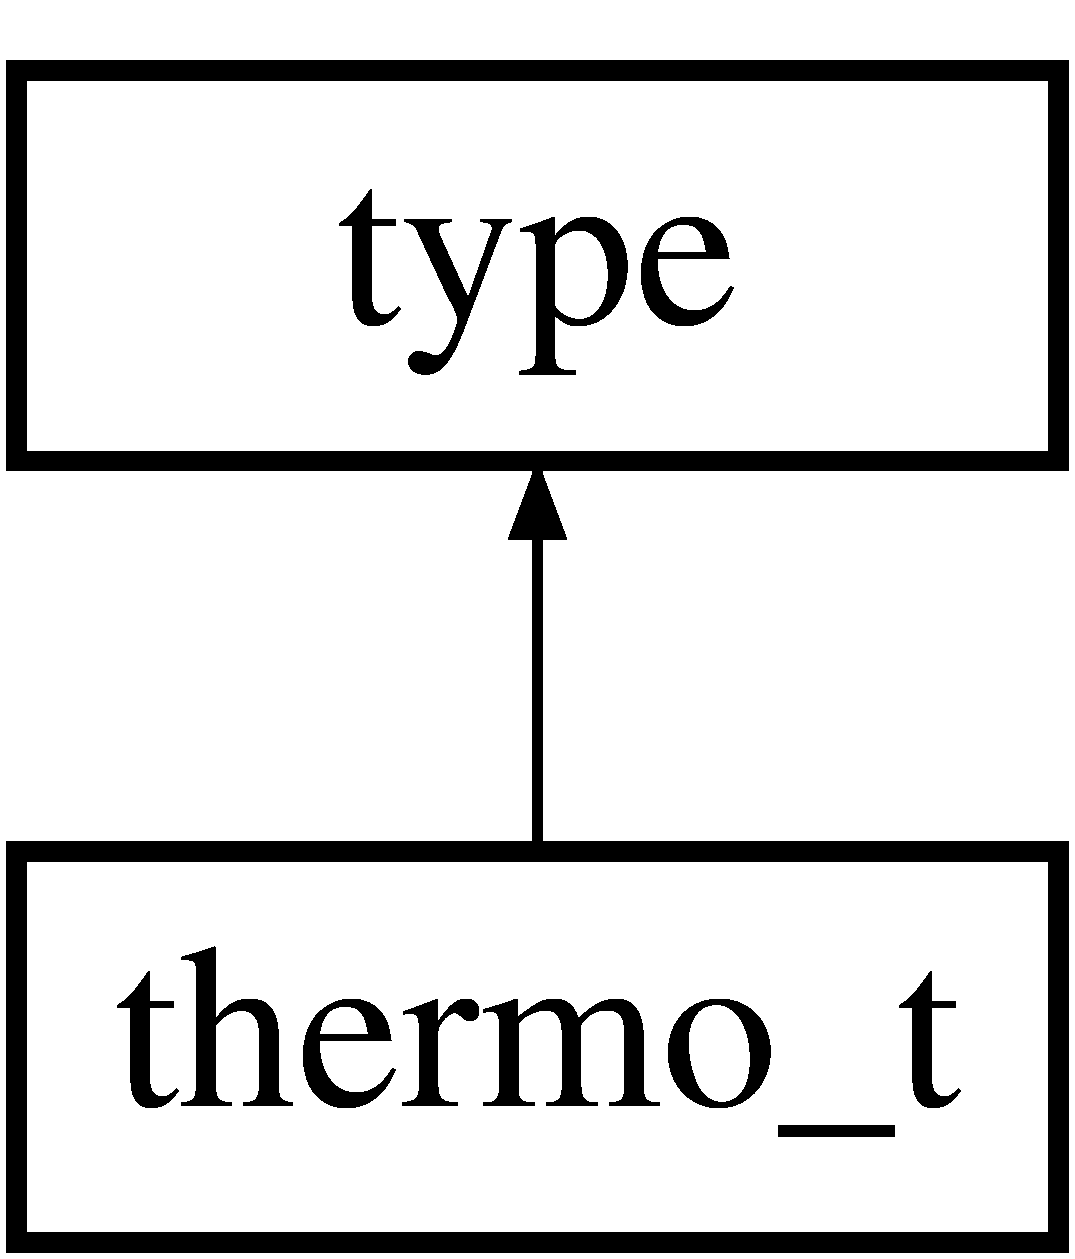
\includegraphics[height=2.000000cm]{classthermo__t}
\end{center}
\end{figure}
\subsection*{Public Types}
\begin{DoxyCompactItemize}
\item 
typedef \+::\hyperlink{namespacexml__schema_ad7e04ab17bba0b3fdde43fb79ef6ed87}{xml\+\_\+schema\+::float\+\_\+} \hyperlink{classthermo__t_a3b889c80ce97870a6967ebee963438ed}{initial\+\_\+type}
\item 
typedef \+::xsd\+::cxx\+::tree\+::traits$<$ \hyperlink{classthermo__t_a3b889c80ce97870a6967ebee963438ed}{initial\+\_\+type}, char $>$ \hyperlink{classthermo__t_a857c3d12cdb293a7ec3ea2e2ac52812c}{initial\+\_\+traits}
\item 
typedef \+::\hyperlink{namespacexml__schema_acfa24ac68e1a188e7f44c36f7a158bf4}{xml\+\_\+schema\+::int\+\_\+} \hyperlink{classthermo__t_a6895e9b201424e2fada14df933774b0c}{timestep\+\_\+type}
\item 
typedef \+::xsd\+::cxx\+::tree\+::traits$<$ \hyperlink{classthermo__t_a6895e9b201424e2fada14df933774b0c}{timestep\+\_\+type}, char $>$ \hyperlink{classthermo__t_a22923d5493f01433df1b956905308222}{timestep\+\_\+traits}
\item 
typedef \+::\hyperlink{classthermo__target__t}{thermo\+\_\+target\+\_\+t} \hyperlink{classthermo__t_a53d64092b110ebaf8c36a23a2c9c40ec}{heating\+\_\+type}
\item 
typedef \+::xsd\+::cxx\+::tree\+::optional$<$ \hyperlink{classthermo__t_a53d64092b110ebaf8c36a23a2c9c40ec}{heating\+\_\+type} $>$ \hyperlink{classthermo__t_a07769e3087269c95ee4fc162c6bf4341}{heating\+\_\+optional}
\item 
typedef \+::xsd\+::cxx\+::tree\+::traits$<$ \hyperlink{classthermo__t_a53d64092b110ebaf8c36a23a2c9c40ec}{heating\+\_\+type}, char $>$ \hyperlink{classthermo__t_adb14cdd53e4543425bb71da6fbb034d5}{heating\+\_\+traits}
\item 
typedef \+::\hyperlink{namespacexml__schema_ae5ada4ec9c54b51765c3e4c0e9631bba}{xml\+\_\+schema\+::boolean} \hyperlink{classthermo__t_a20faf1f752e18e7d9e8f2f7b943fbf01}{ignore\+Y\+\_\+type}
\item 
typedef \+::xsd\+::cxx\+::tree\+::optional$<$ \hyperlink{classthermo__t_a20faf1f752e18e7d9e8f2f7b943fbf01}{ignore\+Y\+\_\+type} $>$ \hyperlink{classthermo__t_a95e0efa769cf6e41e4851c821fde82a9}{ignore\+Y\+\_\+optional}
\item 
typedef \+::xsd\+::cxx\+::tree\+::traits$<$ \hyperlink{classthermo__t_a20faf1f752e18e7d9e8f2f7b943fbf01}{ignore\+Y\+\_\+type}, char $>$ \hyperlink{classthermo__t_a73de5c924d01c03f5d5dda8f571a2f9b}{ignore\+Y\+\_\+traits}
\end{DoxyCompactItemize}
\subsection*{Public Member Functions}
\begin{DoxyCompactItemize}
\item 
const \hyperlink{classthermo__t_a3b889c80ce97870a6967ebee963438ed}{initial\+\_\+type} \& \hyperlink{classthermo__t_a279984e2d428ca1cdc75b599647a1a13}{initial} () const 
\item 
\hyperlink{classthermo__t_a3b889c80ce97870a6967ebee963438ed}{initial\+\_\+type} \& \hyperlink{classthermo__t_a07569ef2c98506acafb4d45cf2ba3007}{initial} ()
\item 
void \hyperlink{classthermo__t_a4e612c1cc79e5b7910e5a8aab33769e8}{initial} (const \hyperlink{classthermo__t_a3b889c80ce97870a6967ebee963438ed}{initial\+\_\+type} \&x)
\item 
const \hyperlink{classthermo__t_a6895e9b201424e2fada14df933774b0c}{timestep\+\_\+type} \& \hyperlink{classthermo__t_a4eb690c69691f503eb8798729950a0bc}{timestep} () const 
\item 
\hyperlink{classthermo__t_a6895e9b201424e2fada14df933774b0c}{timestep\+\_\+type} \& \hyperlink{classthermo__t_aa0b0b27613dc49acab5e36bf23d75a62}{timestep} ()
\item 
void \hyperlink{classthermo__t_afcb6e9f9b2940fb8ac8bcd8d9e155101}{timestep} (const \hyperlink{classthermo__t_a6895e9b201424e2fada14df933774b0c}{timestep\+\_\+type} \&x)
\item 
const \hyperlink{classthermo__t_a07769e3087269c95ee4fc162c6bf4341}{heating\+\_\+optional} \& \hyperlink{classthermo__t_a969cfd3ae1e0384ef167460d6e7f49a4}{heating} () const 
\item 
\hyperlink{classthermo__t_a07769e3087269c95ee4fc162c6bf4341}{heating\+\_\+optional} \& \hyperlink{classthermo__t_a7d238a6312e96860cb90a4a4a9fc8c81}{heating} ()
\item 
void \hyperlink{classthermo__t_a6304d053b24451d70535b6c4a9e216b7}{heating} (const \hyperlink{classthermo__t_a53d64092b110ebaf8c36a23a2c9c40ec}{heating\+\_\+type} \&x)
\item 
void \hyperlink{classthermo__t_a1cf016365963f545536e19be13712bb3}{heating} (const \hyperlink{classthermo__t_a07769e3087269c95ee4fc162c6bf4341}{heating\+\_\+optional} \&x)
\item 
void \hyperlink{classthermo__t_ae78c9120bb615a064bc6b7d35ec0e852}{heating} (\+::std\+::unique\+\_\+ptr$<$ \hyperlink{classthermo__t_a53d64092b110ebaf8c36a23a2c9c40ec}{heating\+\_\+type} $>$ p)
\item 
const \hyperlink{classthermo__t_a95e0efa769cf6e41e4851c821fde82a9}{ignore\+Y\+\_\+optional} \& \hyperlink{classthermo__t_aefb4116e31e4dd7586b915cd68dcd4c0}{ignoreY} () const 
\item 
\hyperlink{classthermo__t_a95e0efa769cf6e41e4851c821fde82a9}{ignore\+Y\+\_\+optional} \& \hyperlink{classthermo__t_ae6ae1b900ac23e51131d1243f177c825}{ignoreY} ()
\item 
void \hyperlink{classthermo__t_a32ec95928025c06fa81693a9d2c3672a}{ignoreY} (const \hyperlink{classthermo__t_a20faf1f752e18e7d9e8f2f7b943fbf01}{ignore\+Y\+\_\+type} \&x)
\item 
void \hyperlink{classthermo__t_a8fc0c14a4f1f52341cefe7518fb10ed0}{ignoreY} (const \hyperlink{classthermo__t_a95e0efa769cf6e41e4851c821fde82a9}{ignore\+Y\+\_\+optional} \&x)
\item 
\hyperlink{classthermo__t_af1527d191e02d46a08f146feb12fcf74}{thermo\+\_\+t} (const \hyperlink{classthermo__t_a3b889c80ce97870a6967ebee963438ed}{initial\+\_\+type} \&, const \hyperlink{classthermo__t_a6895e9b201424e2fada14df933774b0c}{timestep\+\_\+type} \&)
\item 
\hyperlink{classthermo__t_a9d2453469c50d26154ad9126e93da768}{thermo\+\_\+t} (const \+::xercesc\+::\+D\+O\+M\+Element \&e,\+::\hyperlink{namespacexml__schema_a0612287d030cb2732d31a45b258fdc87}{xml\+\_\+schema\+::flags} f=0,\+::\hyperlink{namespacexml__schema_ada9aa30dc722e93ee2ed7243085402a5}{xml\+\_\+schema\+::container} $\ast$c=0)
\item 
\hyperlink{classthermo__t_a524ba6dfc3781a5ee2a86e674097ff00}{thermo\+\_\+t} (const \hyperlink{classthermo__t}{thermo\+\_\+t} \&x,\+::\hyperlink{namespacexml__schema_a0612287d030cb2732d31a45b258fdc87}{xml\+\_\+schema\+::flags} f=0,\+::\hyperlink{namespacexml__schema_ada9aa30dc722e93ee2ed7243085402a5}{xml\+\_\+schema\+::container} $\ast$c=0)
\item 
virtual \hyperlink{classthermo__t}{thermo\+\_\+t} $\ast$ \hyperlink{classthermo__t_a879a6032b26ce6be5227b0f9841401c2}{\+\_\+clone} (\+::\hyperlink{namespacexml__schema_a0612287d030cb2732d31a45b258fdc87}{xml\+\_\+schema\+::flags} f=0,\+::\hyperlink{namespacexml__schema_ada9aa30dc722e93ee2ed7243085402a5}{xml\+\_\+schema\+::container} $\ast$c=0) const 
\item 
\hyperlink{classthermo__t}{thermo\+\_\+t} \& \hyperlink{classthermo__t_af17439150b657be91fdece5590d29877}{operator=} (const \hyperlink{classthermo__t}{thermo\+\_\+t} \&x)
\item 
virtual \hyperlink{classthermo__t_af1f580af388c6d697df6fe432928e7c3}{$\sim$thermo\+\_\+t} ()
\end{DoxyCompactItemize}
\subsection*{Protected Member Functions}
\begin{DoxyCompactItemize}
\item 
void \hyperlink{classthermo__t_ad904ca357fb42ae48a78d887fecf1f00}{parse} (\+::xsd\+::cxx\+::xml\+::dom\+::parser$<$ char $>$ \&,\+::\hyperlink{namespacexml__schema_a0612287d030cb2732d31a45b258fdc87}{xml\+\_\+schema\+::flags})
\end{DoxyCompactItemize}
\subsection*{Protected Attributes}
\begin{DoxyCompactItemize}
\item 
\+::xsd\+::cxx\+::tree\+::one$<$ \hyperlink{classthermo__t_a3b889c80ce97870a6967ebee963438ed}{initial\+\_\+type} $>$ \hyperlink{classthermo__t_a44b9944e39c14f6ad14dc4367b913e17}{initial\+\_\+}
\item 
\+::xsd\+::cxx\+::tree\+::one$<$ \hyperlink{classthermo__t_a6895e9b201424e2fada14df933774b0c}{timestep\+\_\+type} $>$ \hyperlink{classthermo__t_a81482a5b9787aef0293b763d929cfc31}{timestep\+\_\+}
\item 
\hyperlink{classthermo__t_a07769e3087269c95ee4fc162c6bf4341}{heating\+\_\+optional} \hyperlink{classthermo__t_a416f5bd41ef13d1b555d7c441e47ec94}{heating\+\_\+}
\item 
\hyperlink{classthermo__t_a95e0efa769cf6e41e4851c821fde82a9}{ignore\+Y\+\_\+optional} \hyperlink{classthermo__t_a25f092948e00faf10758e74c3930cbcf}{ignore\+Y\+\_\+}
\end{DoxyCompactItemize}


\subsection{Member Typedef Documentation}
\index{thermo\+\_\+t@{thermo\+\_\+t}!heating\+\_\+optional@{heating\+\_\+optional}}
\index{heating\+\_\+optional@{heating\+\_\+optional}!thermo\+\_\+t@{thermo\+\_\+t}}
\subsubsection[{\texorpdfstring{heating\+\_\+optional}{heating_optional}}]{\setlength{\rightskip}{0pt plus 5cm}typedef \+::xsd\+::cxx\+::tree\+::optional$<$ {\bf heating\+\_\+type} $>$ {\bf thermo\+\_\+t\+::heating\+\_\+optional}}\hypertarget{classthermo__t_a07769e3087269c95ee4fc162c6bf4341}{}\label{classthermo__t_a07769e3087269c95ee4fc162c6bf4341}
\index{thermo\+\_\+t@{thermo\+\_\+t}!heating\+\_\+traits@{heating\+\_\+traits}}
\index{heating\+\_\+traits@{heating\+\_\+traits}!thermo\+\_\+t@{thermo\+\_\+t}}
\subsubsection[{\texorpdfstring{heating\+\_\+traits}{heating_traits}}]{\setlength{\rightskip}{0pt plus 5cm}typedef \+::xsd\+::cxx\+::tree\+::traits$<$ {\bf heating\+\_\+type}, char $>$ {\bf thermo\+\_\+t\+::heating\+\_\+traits}}\hypertarget{classthermo__t_adb14cdd53e4543425bb71da6fbb034d5}{}\label{classthermo__t_adb14cdd53e4543425bb71da6fbb034d5}
\index{thermo\+\_\+t@{thermo\+\_\+t}!heating\+\_\+type@{heating\+\_\+type}}
\index{heating\+\_\+type@{heating\+\_\+type}!thermo\+\_\+t@{thermo\+\_\+t}}
\subsubsection[{\texorpdfstring{heating\+\_\+type}{heating_type}}]{\setlength{\rightskip}{0pt plus 5cm}typedef \+::{\bf thermo\+\_\+target\+\_\+t} {\bf thermo\+\_\+t\+::heating\+\_\+type}}\hypertarget{classthermo__t_a53d64092b110ebaf8c36a23a2c9c40ec}{}\label{classthermo__t_a53d64092b110ebaf8c36a23a2c9c40ec}
\index{thermo\+\_\+t@{thermo\+\_\+t}!ignore\+Y\+\_\+optional@{ignore\+Y\+\_\+optional}}
\index{ignore\+Y\+\_\+optional@{ignore\+Y\+\_\+optional}!thermo\+\_\+t@{thermo\+\_\+t}}
\subsubsection[{\texorpdfstring{ignore\+Y\+\_\+optional}{ignoreY_optional}}]{\setlength{\rightskip}{0pt plus 5cm}typedef \+::xsd\+::cxx\+::tree\+::optional$<$ {\bf ignore\+Y\+\_\+type} $>$ {\bf thermo\+\_\+t\+::ignore\+Y\+\_\+optional}}\hypertarget{classthermo__t_a95e0efa769cf6e41e4851c821fde82a9}{}\label{classthermo__t_a95e0efa769cf6e41e4851c821fde82a9}
\index{thermo\+\_\+t@{thermo\+\_\+t}!ignore\+Y\+\_\+traits@{ignore\+Y\+\_\+traits}}
\index{ignore\+Y\+\_\+traits@{ignore\+Y\+\_\+traits}!thermo\+\_\+t@{thermo\+\_\+t}}
\subsubsection[{\texorpdfstring{ignore\+Y\+\_\+traits}{ignoreY_traits}}]{\setlength{\rightskip}{0pt plus 5cm}typedef \+::xsd\+::cxx\+::tree\+::traits$<$ {\bf ignore\+Y\+\_\+type}, char $>$ {\bf thermo\+\_\+t\+::ignore\+Y\+\_\+traits}}\hypertarget{classthermo__t_a73de5c924d01c03f5d5dda8f571a2f9b}{}\label{classthermo__t_a73de5c924d01c03f5d5dda8f571a2f9b}
\index{thermo\+\_\+t@{thermo\+\_\+t}!ignore\+Y\+\_\+type@{ignore\+Y\+\_\+type}}
\index{ignore\+Y\+\_\+type@{ignore\+Y\+\_\+type}!thermo\+\_\+t@{thermo\+\_\+t}}
\subsubsection[{\texorpdfstring{ignore\+Y\+\_\+type}{ignoreY_type}}]{\setlength{\rightskip}{0pt plus 5cm}typedef \+::{\bf xml\+\_\+schema\+::boolean} {\bf thermo\+\_\+t\+::ignore\+Y\+\_\+type}}\hypertarget{classthermo__t_a20faf1f752e18e7d9e8f2f7b943fbf01}{}\label{classthermo__t_a20faf1f752e18e7d9e8f2f7b943fbf01}
\index{thermo\+\_\+t@{thermo\+\_\+t}!initial\+\_\+traits@{initial\+\_\+traits}}
\index{initial\+\_\+traits@{initial\+\_\+traits}!thermo\+\_\+t@{thermo\+\_\+t}}
\subsubsection[{\texorpdfstring{initial\+\_\+traits}{initial_traits}}]{\setlength{\rightskip}{0pt plus 5cm}typedef \+::xsd\+::cxx\+::tree\+::traits$<$ {\bf initial\+\_\+type}, char $>$ {\bf thermo\+\_\+t\+::initial\+\_\+traits}}\hypertarget{classthermo__t_a857c3d12cdb293a7ec3ea2e2ac52812c}{}\label{classthermo__t_a857c3d12cdb293a7ec3ea2e2ac52812c}
\index{thermo\+\_\+t@{thermo\+\_\+t}!initial\+\_\+type@{initial\+\_\+type}}
\index{initial\+\_\+type@{initial\+\_\+type}!thermo\+\_\+t@{thermo\+\_\+t}}
\subsubsection[{\texorpdfstring{initial\+\_\+type}{initial_type}}]{\setlength{\rightskip}{0pt plus 5cm}typedef \+::{\bf xml\+\_\+schema\+::float\+\_\+} {\bf thermo\+\_\+t\+::initial\+\_\+type}}\hypertarget{classthermo__t_a3b889c80ce97870a6967ebee963438ed}{}\label{classthermo__t_a3b889c80ce97870a6967ebee963438ed}
\index{thermo\+\_\+t@{thermo\+\_\+t}!timestep\+\_\+traits@{timestep\+\_\+traits}}
\index{timestep\+\_\+traits@{timestep\+\_\+traits}!thermo\+\_\+t@{thermo\+\_\+t}}
\subsubsection[{\texorpdfstring{timestep\+\_\+traits}{timestep_traits}}]{\setlength{\rightskip}{0pt plus 5cm}typedef \+::xsd\+::cxx\+::tree\+::traits$<$ {\bf timestep\+\_\+type}, char $>$ {\bf thermo\+\_\+t\+::timestep\+\_\+traits}}\hypertarget{classthermo__t_a22923d5493f01433df1b956905308222}{}\label{classthermo__t_a22923d5493f01433df1b956905308222}
\index{thermo\+\_\+t@{thermo\+\_\+t}!timestep\+\_\+type@{timestep\+\_\+type}}
\index{timestep\+\_\+type@{timestep\+\_\+type}!thermo\+\_\+t@{thermo\+\_\+t}}
\subsubsection[{\texorpdfstring{timestep\+\_\+type}{timestep_type}}]{\setlength{\rightskip}{0pt plus 5cm}typedef \+::{\bf xml\+\_\+schema\+::int\+\_\+} {\bf thermo\+\_\+t\+::timestep\+\_\+type}}\hypertarget{classthermo__t_a6895e9b201424e2fada14df933774b0c}{}\label{classthermo__t_a6895e9b201424e2fada14df933774b0c}


\subsection{Constructor \& Destructor Documentation}
\index{thermo\+\_\+t@{thermo\+\_\+t}!thermo\+\_\+t@{thermo\+\_\+t}}
\index{thermo\+\_\+t@{thermo\+\_\+t}!thermo\+\_\+t@{thermo\+\_\+t}}
\subsubsection[{\texorpdfstring{thermo\+\_\+t(const initial\+\_\+type \&, const timestep\+\_\+type \&)}{thermo_t(const initial_type &, const timestep_type &)}}]{\setlength{\rightskip}{0pt plus 5cm}thermo\+\_\+t\+::thermo\+\_\+t (
\begin{DoxyParamCaption}
\item[{const {\bf initial\+\_\+type} \&}]{initial, }
\item[{const {\bf timestep\+\_\+type} \&}]{timestep}
\end{DoxyParamCaption}
)}\hypertarget{classthermo__t_af1527d191e02d46a08f146feb12fcf74}{}\label{classthermo__t_af1527d191e02d46a08f146feb12fcf74}
\index{thermo\+\_\+t@{thermo\+\_\+t}!thermo\+\_\+t@{thermo\+\_\+t}}
\index{thermo\+\_\+t@{thermo\+\_\+t}!thermo\+\_\+t@{thermo\+\_\+t}}
\subsubsection[{\texorpdfstring{thermo\+\_\+t(const \+::xercesc\+::\+D\+O\+M\+Element \&e,\+::xml\+\_\+schema\+::flags f=0,\+::xml\+\_\+schema\+::container $\ast$c=0)}{thermo_t(const ::xercesc::DOMElement &e,::xml_schema::flags f=0,::xml_schema::container *c=0)}}]{\setlength{\rightskip}{0pt plus 5cm}thermo\+\_\+t\+::thermo\+\_\+t (
\begin{DoxyParamCaption}
\item[{const \+::xercesc\+::\+D\+O\+M\+Element \&}]{e, }
\item[{\+::{\bf xml\+\_\+schema\+::flags}}]{f = {\ttfamily 0}, }
\item[{\+::{\bf xml\+\_\+schema\+::container} $\ast$}]{c = {\ttfamily 0}}
\end{DoxyParamCaption}
)}\hypertarget{classthermo__t_a9d2453469c50d26154ad9126e93da768}{}\label{classthermo__t_a9d2453469c50d26154ad9126e93da768}
\index{thermo\+\_\+t@{thermo\+\_\+t}!thermo\+\_\+t@{thermo\+\_\+t}}
\index{thermo\+\_\+t@{thermo\+\_\+t}!thermo\+\_\+t@{thermo\+\_\+t}}
\subsubsection[{\texorpdfstring{thermo\+\_\+t(const thermo\+\_\+t \&x,\+::xml\+\_\+schema\+::flags f=0,\+::xml\+\_\+schema\+::container $\ast$c=0)}{thermo_t(const thermo_t &x,::xml_schema::flags f=0,::xml_schema::container *c=0)}}]{\setlength{\rightskip}{0pt plus 5cm}thermo\+\_\+t\+::thermo\+\_\+t (
\begin{DoxyParamCaption}
\item[{const {\bf thermo\+\_\+t} \&}]{x, }
\item[{\+::{\bf xml\+\_\+schema\+::flags}}]{f = {\ttfamily 0}, }
\item[{\+::{\bf xml\+\_\+schema\+::container} $\ast$}]{c = {\ttfamily 0}}
\end{DoxyParamCaption}
)}\hypertarget{classthermo__t_a524ba6dfc3781a5ee2a86e674097ff00}{}\label{classthermo__t_a524ba6dfc3781a5ee2a86e674097ff00}
\index{thermo\+\_\+t@{thermo\+\_\+t}!````~thermo\+\_\+t@{$\sim$thermo\+\_\+t}}
\index{````~thermo\+\_\+t@{$\sim$thermo\+\_\+t}!thermo\+\_\+t@{thermo\+\_\+t}}
\subsubsection[{\texorpdfstring{$\sim$thermo\+\_\+t()}{~thermo_t()}}]{\setlength{\rightskip}{0pt plus 5cm}thermo\+\_\+t\+::$\sim$thermo\+\_\+t (
\begin{DoxyParamCaption}
{}
\end{DoxyParamCaption}
)\hspace{0.3cm}{\ttfamily [virtual]}}\hypertarget{classthermo__t_af1f580af388c6d697df6fe432928e7c3}{}\label{classthermo__t_af1f580af388c6d697df6fe432928e7c3}


\subsection{Member Function Documentation}
\index{thermo\+\_\+t@{thermo\+\_\+t}!\+\_\+clone@{\+\_\+clone}}
\index{\+\_\+clone@{\+\_\+clone}!thermo\+\_\+t@{thermo\+\_\+t}}
\subsubsection[{\texorpdfstring{\+\_\+clone(\+::xml\+\_\+schema\+::flags f=0,\+::xml\+\_\+schema\+::container $\ast$c=0) const }{_clone(::xml_schema::flags f=0,::xml_schema::container *c=0) const }}]{\setlength{\rightskip}{0pt plus 5cm}{\bf thermo\+\_\+t} $\ast$ thermo\+\_\+t\+::\+\_\+clone (
\begin{DoxyParamCaption}
\item[{\+::{\bf xml\+\_\+schema\+::flags}}]{f = {\ttfamily 0}, }
\item[{\+::{\bf xml\+\_\+schema\+::container} $\ast$}]{c = {\ttfamily 0}}
\end{DoxyParamCaption}
) const\hspace{0.3cm}{\ttfamily [virtual]}}\hypertarget{classthermo__t_a879a6032b26ce6be5227b0f9841401c2}{}\label{classthermo__t_a879a6032b26ce6be5227b0f9841401c2}
\index{thermo\+\_\+t@{thermo\+\_\+t}!heating@{heating}}
\index{heating@{heating}!thermo\+\_\+t@{thermo\+\_\+t}}
\subsubsection[{\texorpdfstring{heating() const }{heating() const }}]{\setlength{\rightskip}{0pt plus 5cm}const {\bf thermo\+\_\+t\+::heating\+\_\+optional} \& thermo\+\_\+t\+::heating (
\begin{DoxyParamCaption}
{}
\end{DoxyParamCaption}
) const}\hypertarget{classthermo__t_a969cfd3ae1e0384ef167460d6e7f49a4}{}\label{classthermo__t_a969cfd3ae1e0384ef167460d6e7f49a4}
\index{thermo\+\_\+t@{thermo\+\_\+t}!heating@{heating}}
\index{heating@{heating}!thermo\+\_\+t@{thermo\+\_\+t}}
\subsubsection[{\texorpdfstring{heating()}{heating()}}]{\setlength{\rightskip}{0pt plus 5cm}{\bf thermo\+\_\+t\+::heating\+\_\+optional} \& thermo\+\_\+t\+::heating (
\begin{DoxyParamCaption}
{}
\end{DoxyParamCaption}
)}\hypertarget{classthermo__t_a7d238a6312e96860cb90a4a4a9fc8c81}{}\label{classthermo__t_a7d238a6312e96860cb90a4a4a9fc8c81}
\index{thermo\+\_\+t@{thermo\+\_\+t}!heating@{heating}}
\index{heating@{heating}!thermo\+\_\+t@{thermo\+\_\+t}}
\subsubsection[{\texorpdfstring{heating(const heating\+\_\+type \&x)}{heating(const heating_type &x)}}]{\setlength{\rightskip}{0pt plus 5cm}void thermo\+\_\+t\+::heating (
\begin{DoxyParamCaption}
\item[{const {\bf heating\+\_\+type} \&}]{x}
\end{DoxyParamCaption}
)}\hypertarget{classthermo__t_a6304d053b24451d70535b6c4a9e216b7}{}\label{classthermo__t_a6304d053b24451d70535b6c4a9e216b7}
\index{thermo\+\_\+t@{thermo\+\_\+t}!heating@{heating}}
\index{heating@{heating}!thermo\+\_\+t@{thermo\+\_\+t}}
\subsubsection[{\texorpdfstring{heating(const heating\+\_\+optional \&x)}{heating(const heating_optional &x)}}]{\setlength{\rightskip}{0pt plus 5cm}void thermo\+\_\+t\+::heating (
\begin{DoxyParamCaption}
\item[{const {\bf heating\+\_\+optional} \&}]{x}
\end{DoxyParamCaption}
)}\hypertarget{classthermo__t_a1cf016365963f545536e19be13712bb3}{}\label{classthermo__t_a1cf016365963f545536e19be13712bb3}
\index{thermo\+\_\+t@{thermo\+\_\+t}!heating@{heating}}
\index{heating@{heating}!thermo\+\_\+t@{thermo\+\_\+t}}
\subsubsection[{\texorpdfstring{heating(\+::std\+::unique\+\_\+ptr$<$ heating\+\_\+type $>$ p)}{heating(::std::unique_ptr< heating_type > p)}}]{\setlength{\rightskip}{0pt plus 5cm}void thermo\+\_\+t\+::heating (
\begin{DoxyParamCaption}
\item[{\+::std\+::unique\+\_\+ptr$<$ {\bf heating\+\_\+type} $>$}]{p}
\end{DoxyParamCaption}
)}\hypertarget{classthermo__t_ae78c9120bb615a064bc6b7d35ec0e852}{}\label{classthermo__t_ae78c9120bb615a064bc6b7d35ec0e852}
\index{thermo\+\_\+t@{thermo\+\_\+t}!ignoreY@{ignoreY}}
\index{ignoreY@{ignoreY}!thermo\+\_\+t@{thermo\+\_\+t}}
\subsubsection[{\texorpdfstring{ignore\+Y() const }{ignoreY() const }}]{\setlength{\rightskip}{0pt plus 5cm}const {\bf thermo\+\_\+t\+::ignore\+Y\+\_\+optional} \& thermo\+\_\+t\+::ignoreY (
\begin{DoxyParamCaption}
{}
\end{DoxyParamCaption}
) const}\hypertarget{classthermo__t_aefb4116e31e4dd7586b915cd68dcd4c0}{}\label{classthermo__t_aefb4116e31e4dd7586b915cd68dcd4c0}
\index{thermo\+\_\+t@{thermo\+\_\+t}!ignoreY@{ignoreY}}
\index{ignoreY@{ignoreY}!thermo\+\_\+t@{thermo\+\_\+t}}
\subsubsection[{\texorpdfstring{ignore\+Y()}{ignoreY()}}]{\setlength{\rightskip}{0pt plus 5cm}{\bf thermo\+\_\+t\+::ignore\+Y\+\_\+optional} \& thermo\+\_\+t\+::ignoreY (
\begin{DoxyParamCaption}
{}
\end{DoxyParamCaption}
)}\hypertarget{classthermo__t_ae6ae1b900ac23e51131d1243f177c825}{}\label{classthermo__t_ae6ae1b900ac23e51131d1243f177c825}
\index{thermo\+\_\+t@{thermo\+\_\+t}!ignoreY@{ignoreY}}
\index{ignoreY@{ignoreY}!thermo\+\_\+t@{thermo\+\_\+t}}
\subsubsection[{\texorpdfstring{ignore\+Y(const ignore\+Y\+\_\+type \&x)}{ignoreY(const ignoreY_type &x)}}]{\setlength{\rightskip}{0pt plus 5cm}void thermo\+\_\+t\+::ignoreY (
\begin{DoxyParamCaption}
\item[{const {\bf ignore\+Y\+\_\+type} \&}]{x}
\end{DoxyParamCaption}
)}\hypertarget{classthermo__t_a32ec95928025c06fa81693a9d2c3672a}{}\label{classthermo__t_a32ec95928025c06fa81693a9d2c3672a}
\index{thermo\+\_\+t@{thermo\+\_\+t}!ignoreY@{ignoreY}}
\index{ignoreY@{ignoreY}!thermo\+\_\+t@{thermo\+\_\+t}}
\subsubsection[{\texorpdfstring{ignore\+Y(const ignore\+Y\+\_\+optional \&x)}{ignoreY(const ignoreY_optional &x)}}]{\setlength{\rightskip}{0pt plus 5cm}void thermo\+\_\+t\+::ignoreY (
\begin{DoxyParamCaption}
\item[{const {\bf ignore\+Y\+\_\+optional} \&}]{x}
\end{DoxyParamCaption}
)}\hypertarget{classthermo__t_a8fc0c14a4f1f52341cefe7518fb10ed0}{}\label{classthermo__t_a8fc0c14a4f1f52341cefe7518fb10ed0}
\index{thermo\+\_\+t@{thermo\+\_\+t}!initial@{initial}}
\index{initial@{initial}!thermo\+\_\+t@{thermo\+\_\+t}}
\subsubsection[{\texorpdfstring{initial() const }{initial() const }}]{\setlength{\rightskip}{0pt plus 5cm}const {\bf thermo\+\_\+t\+::initial\+\_\+type} \& thermo\+\_\+t\+::initial (
\begin{DoxyParamCaption}
{}
\end{DoxyParamCaption}
) const}\hypertarget{classthermo__t_a279984e2d428ca1cdc75b599647a1a13}{}\label{classthermo__t_a279984e2d428ca1cdc75b599647a1a13}
\index{thermo\+\_\+t@{thermo\+\_\+t}!initial@{initial}}
\index{initial@{initial}!thermo\+\_\+t@{thermo\+\_\+t}}
\subsubsection[{\texorpdfstring{initial()}{initial()}}]{\setlength{\rightskip}{0pt plus 5cm}{\bf thermo\+\_\+t\+::initial\+\_\+type} \& thermo\+\_\+t\+::initial (
\begin{DoxyParamCaption}
{}
\end{DoxyParamCaption}
)}\hypertarget{classthermo__t_a07569ef2c98506acafb4d45cf2ba3007}{}\label{classthermo__t_a07569ef2c98506acafb4d45cf2ba3007}
\index{thermo\+\_\+t@{thermo\+\_\+t}!initial@{initial}}
\index{initial@{initial}!thermo\+\_\+t@{thermo\+\_\+t}}
\subsubsection[{\texorpdfstring{initial(const initial\+\_\+type \&x)}{initial(const initial_type &x)}}]{\setlength{\rightskip}{0pt plus 5cm}void thermo\+\_\+t\+::initial (
\begin{DoxyParamCaption}
\item[{const {\bf initial\+\_\+type} \&}]{x}
\end{DoxyParamCaption}
)}\hypertarget{classthermo__t_a4e612c1cc79e5b7910e5a8aab33769e8}{}\label{classthermo__t_a4e612c1cc79e5b7910e5a8aab33769e8}
\index{thermo\+\_\+t@{thermo\+\_\+t}!operator=@{operator=}}
\index{operator=@{operator=}!thermo\+\_\+t@{thermo\+\_\+t}}
\subsubsection[{\texorpdfstring{operator=(const thermo\+\_\+t \&x)}{operator=(const thermo_t &x)}}]{\setlength{\rightskip}{0pt plus 5cm}{\bf thermo\+\_\+t} \& thermo\+\_\+t\+::operator= (
\begin{DoxyParamCaption}
\item[{const {\bf thermo\+\_\+t} \&}]{x}
\end{DoxyParamCaption}
)}\hypertarget{classthermo__t_af17439150b657be91fdece5590d29877}{}\label{classthermo__t_af17439150b657be91fdece5590d29877}
\index{thermo\+\_\+t@{thermo\+\_\+t}!parse@{parse}}
\index{parse@{parse}!thermo\+\_\+t@{thermo\+\_\+t}}
\subsubsection[{\texorpdfstring{parse(\+::xsd\+::cxx\+::xml\+::dom\+::parser$<$ char $>$ \&,\+::xml\+\_\+schema\+::flags)}{parse(::xsd::cxx::xml::dom::parser< char > &,::xml_schema::flags)}}]{\setlength{\rightskip}{0pt plus 5cm}void thermo\+\_\+t\+::parse (
\begin{DoxyParamCaption}
\item[{\+::xsd\+::cxx\+::xml\+::dom\+::parser$<$ char $>$ \&}]{p, }
\item[{\+::{\bf xml\+\_\+schema\+::flags}}]{f}
\end{DoxyParamCaption}
)\hspace{0.3cm}{\ttfamily [protected]}}\hypertarget{classthermo__t_ad904ca357fb42ae48a78d887fecf1f00}{}\label{classthermo__t_ad904ca357fb42ae48a78d887fecf1f00}
\index{thermo\+\_\+t@{thermo\+\_\+t}!timestep@{timestep}}
\index{timestep@{timestep}!thermo\+\_\+t@{thermo\+\_\+t}}
\subsubsection[{\texorpdfstring{timestep() const }{timestep() const }}]{\setlength{\rightskip}{0pt plus 5cm}const {\bf thermo\+\_\+t\+::timestep\+\_\+type} \& thermo\+\_\+t\+::timestep (
\begin{DoxyParamCaption}
{}
\end{DoxyParamCaption}
) const}\hypertarget{classthermo__t_a4eb690c69691f503eb8798729950a0bc}{}\label{classthermo__t_a4eb690c69691f503eb8798729950a0bc}
\index{thermo\+\_\+t@{thermo\+\_\+t}!timestep@{timestep}}
\index{timestep@{timestep}!thermo\+\_\+t@{thermo\+\_\+t}}
\subsubsection[{\texorpdfstring{timestep()}{timestep()}}]{\setlength{\rightskip}{0pt plus 5cm}{\bf thermo\+\_\+t\+::timestep\+\_\+type} \& thermo\+\_\+t\+::timestep (
\begin{DoxyParamCaption}
{}
\end{DoxyParamCaption}
)}\hypertarget{classthermo__t_aa0b0b27613dc49acab5e36bf23d75a62}{}\label{classthermo__t_aa0b0b27613dc49acab5e36bf23d75a62}
\index{thermo\+\_\+t@{thermo\+\_\+t}!timestep@{timestep}}
\index{timestep@{timestep}!thermo\+\_\+t@{thermo\+\_\+t}}
\subsubsection[{\texorpdfstring{timestep(const timestep\+\_\+type \&x)}{timestep(const timestep_type &x)}}]{\setlength{\rightskip}{0pt plus 5cm}void thermo\+\_\+t\+::timestep (
\begin{DoxyParamCaption}
\item[{const {\bf timestep\+\_\+type} \&}]{x}
\end{DoxyParamCaption}
)}\hypertarget{classthermo__t_afcb6e9f9b2940fb8ac8bcd8d9e155101}{}\label{classthermo__t_afcb6e9f9b2940fb8ac8bcd8d9e155101}


\subsection{Member Data Documentation}
\index{thermo\+\_\+t@{thermo\+\_\+t}!heating\+\_\+@{heating\+\_\+}}
\index{heating\+\_\+@{heating\+\_\+}!thermo\+\_\+t@{thermo\+\_\+t}}
\subsubsection[{\texorpdfstring{heating\+\_\+}{heating_}}]{\setlength{\rightskip}{0pt plus 5cm}{\bf heating\+\_\+optional} thermo\+\_\+t\+::heating\+\_\+\hspace{0.3cm}{\ttfamily [protected]}}\hypertarget{classthermo__t_a416f5bd41ef13d1b555d7c441e47ec94}{}\label{classthermo__t_a416f5bd41ef13d1b555d7c441e47ec94}
\index{thermo\+\_\+t@{thermo\+\_\+t}!ignore\+Y\+\_\+@{ignore\+Y\+\_\+}}
\index{ignore\+Y\+\_\+@{ignore\+Y\+\_\+}!thermo\+\_\+t@{thermo\+\_\+t}}
\subsubsection[{\texorpdfstring{ignore\+Y\+\_\+}{ignoreY_}}]{\setlength{\rightskip}{0pt plus 5cm}{\bf ignore\+Y\+\_\+optional} thermo\+\_\+t\+::ignore\+Y\+\_\+\hspace{0.3cm}{\ttfamily [protected]}}\hypertarget{classthermo__t_a25f092948e00faf10758e74c3930cbcf}{}\label{classthermo__t_a25f092948e00faf10758e74c3930cbcf}
\index{thermo\+\_\+t@{thermo\+\_\+t}!initial\+\_\+@{initial\+\_\+}}
\index{initial\+\_\+@{initial\+\_\+}!thermo\+\_\+t@{thermo\+\_\+t}}
\subsubsection[{\texorpdfstring{initial\+\_\+}{initial_}}]{\setlength{\rightskip}{0pt plus 5cm}\+::xsd\+::cxx\+::tree\+::one$<$ {\bf initial\+\_\+type} $>$ thermo\+\_\+t\+::initial\+\_\+\hspace{0.3cm}{\ttfamily [protected]}}\hypertarget{classthermo__t_a44b9944e39c14f6ad14dc4367b913e17}{}\label{classthermo__t_a44b9944e39c14f6ad14dc4367b913e17}
\index{thermo\+\_\+t@{thermo\+\_\+t}!timestep\+\_\+@{timestep\+\_\+}}
\index{timestep\+\_\+@{timestep\+\_\+}!thermo\+\_\+t@{thermo\+\_\+t}}
\subsubsection[{\texorpdfstring{timestep\+\_\+}{timestep_}}]{\setlength{\rightskip}{0pt plus 5cm}\+::xsd\+::cxx\+::tree\+::one$<$ {\bf timestep\+\_\+type} $>$ thermo\+\_\+t\+::timestep\+\_\+\hspace{0.3cm}{\ttfamily [protected]}}\hypertarget{classthermo__t_a81482a5b9787aef0293b763d929cfc31}{}\label{classthermo__t_a81482a5b9787aef0293b763d929cfc31}


The documentation for this class was generated from the following files\+:\begin{DoxyCompactItemize}
\item 
src/setting/\hyperlink{setting_8h}{setting.\+h}\item 
src/setting/\hyperlink{setting_8cpp}{setting.\+cpp}\end{DoxyCompactItemize}

\hypertarget{classthermo__target__t}{}\section{thermo\+\_\+target\+\_\+t Class Reference}
\label{classthermo__target__t}\index{thermo\+\_\+target\+\_\+t@{thermo\+\_\+target\+\_\+t}}


{\ttfamily \#include $<$setting.\+h$>$}

Inheritance diagram for thermo\+\_\+target\+\_\+t\+:\begin{figure}[H]
\begin{center}
\leavevmode
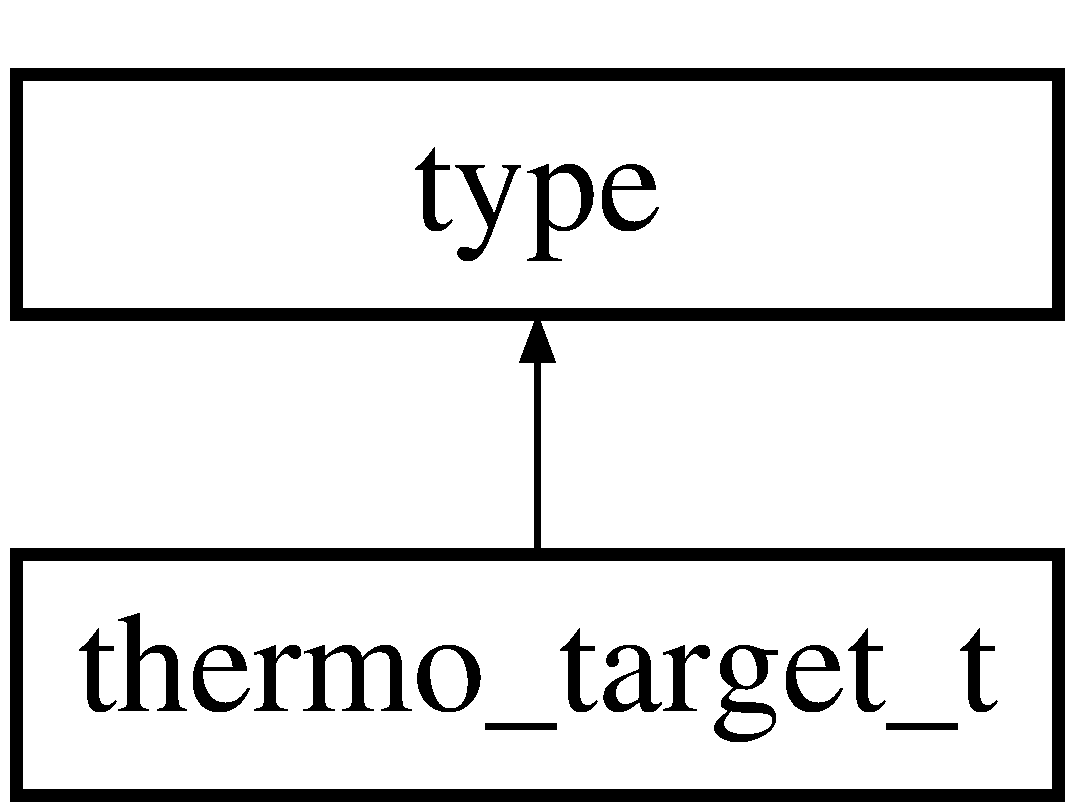
\includegraphics[height=2.000000cm]{classthermo__target__t}
\end{center}
\end{figure}
\subsection*{Public Types}
\begin{DoxyCompactItemize}
\item 
typedef \+::\hyperlink{namespacexml__schema_ad7e04ab17bba0b3fdde43fb79ef6ed87}{xml\+\_\+schema\+::float\+\_\+} \hyperlink{classthermo__target__t_af968c613cbe6e33fcd41b038cefe1f0a}{target\+\_\+type}
\item 
typedef \+::xsd\+::cxx\+::tree\+::traits$<$ \hyperlink{classthermo__target__t_af968c613cbe6e33fcd41b038cefe1f0a}{target\+\_\+type}, char $>$ \hyperlink{classthermo__target__t_a560deecfd869cf48273f19845ab11324}{target\+\_\+traits}
\item 
typedef \+::\hyperlink{namespacexml__schema_ad7e04ab17bba0b3fdde43fb79ef6ed87}{xml\+\_\+schema\+::float\+\_\+} \hyperlink{classthermo__target__t_a55faae5a0c7af8d0e9567600150603b3}{temperature\+\_\+step\+\_\+type}
\item 
typedef \+::xsd\+::cxx\+::tree\+::traits$<$ \hyperlink{classthermo__target__t_a55faae5a0c7af8d0e9567600150603b3}{temperature\+\_\+step\+\_\+type}, char $>$ \hyperlink{classthermo__target__t_a16f117780a400d02f2d96858f362f52a}{temperature\+\_\+step\+\_\+traits}
\item 
typedef \+::\hyperlink{namespacexml__schema_acfa24ac68e1a188e7f44c36f7a158bf4}{xml\+\_\+schema\+::int\+\_\+} \hyperlink{classthermo__target__t_a37e1805b2e121c0e0b0a97b2f5d1dfcb}{timestep\+\_\+type}
\item 
typedef \+::xsd\+::cxx\+::tree\+::traits$<$ \hyperlink{classthermo__target__t_a37e1805b2e121c0e0b0a97b2f5d1dfcb}{timestep\+\_\+type}, char $>$ \hyperlink{classthermo__target__t_a1c37c54b22da31cd1b012efafd0f7d6d}{timestep\+\_\+traits}
\end{DoxyCompactItemize}
\subsection*{Public Member Functions}
\begin{DoxyCompactItemize}
\item 
const \hyperlink{classthermo__target__t_af968c613cbe6e33fcd41b038cefe1f0a}{target\+\_\+type} \& \hyperlink{classthermo__target__t_a628672966d5ead6bc71493e55c34cbb3}{target} () const 
\item 
\hyperlink{classthermo__target__t_af968c613cbe6e33fcd41b038cefe1f0a}{target\+\_\+type} \& \hyperlink{classthermo__target__t_abe08ab311899de79dcd5a8b8fb428633}{target} ()
\item 
void \hyperlink{classthermo__target__t_aece45034721555ad13b977472d99bceb}{target} (const \hyperlink{classthermo__target__t_af968c613cbe6e33fcd41b038cefe1f0a}{target\+\_\+type} \&x)
\item 
const \hyperlink{classthermo__target__t_a55faae5a0c7af8d0e9567600150603b3}{temperature\+\_\+step\+\_\+type} \& \hyperlink{classthermo__target__t_a134cfd51fcc648b9b9c1f57da9d1e262}{temperature\+\_\+step} () const 
\item 
\hyperlink{classthermo__target__t_a55faae5a0c7af8d0e9567600150603b3}{temperature\+\_\+step\+\_\+type} \& \hyperlink{classthermo__target__t_a382ec9ab3ebcdb72d29d67041c78f714}{temperature\+\_\+step} ()
\item 
void \hyperlink{classthermo__target__t_a8b616af6e45e4c9f7c46ca968b1ffe88}{temperature\+\_\+step} (const \hyperlink{classthermo__target__t_a55faae5a0c7af8d0e9567600150603b3}{temperature\+\_\+step\+\_\+type} \&x)
\item 
const \hyperlink{classthermo__target__t_a37e1805b2e121c0e0b0a97b2f5d1dfcb}{timestep\+\_\+type} \& \hyperlink{classthermo__target__t_ab10e13a5b5afda48390aacee846957f7}{timestep} () const 
\item 
\hyperlink{classthermo__target__t_a37e1805b2e121c0e0b0a97b2f5d1dfcb}{timestep\+\_\+type} \& \hyperlink{classthermo__target__t_a489192ff6e44baf14178314b51805c52}{timestep} ()
\item 
void \hyperlink{classthermo__target__t_ad59c4e3d249181e5ddf18eb1c7fab5c0}{timestep} (const \hyperlink{classthermo__target__t_a37e1805b2e121c0e0b0a97b2f5d1dfcb}{timestep\+\_\+type} \&x)
\item 
\hyperlink{classthermo__target__t_a11b7af954c7b09a69d0edd1d44be7828}{thermo\+\_\+target\+\_\+t} (const \hyperlink{classthermo__target__t_af968c613cbe6e33fcd41b038cefe1f0a}{target\+\_\+type} \&, const \hyperlink{classthermo__target__t_a55faae5a0c7af8d0e9567600150603b3}{temperature\+\_\+step\+\_\+type} \&, const \hyperlink{classthermo__target__t_a37e1805b2e121c0e0b0a97b2f5d1dfcb}{timestep\+\_\+type} \&)
\item 
\hyperlink{classthermo__target__t_a9ac3b10f9c5654e81cba5276195c38a1}{thermo\+\_\+target\+\_\+t} (const \+::xercesc\+::\+D\+O\+M\+Element \&e,\+::\hyperlink{namespacexml__schema_a0612287d030cb2732d31a45b258fdc87}{xml\+\_\+schema\+::flags} f=0,\+::\hyperlink{namespacexml__schema_ada9aa30dc722e93ee2ed7243085402a5}{xml\+\_\+schema\+::container} $\ast$c=0)
\item 
\hyperlink{classthermo__target__t_ab7e1761c001576d9a8d487b0915338ee}{thermo\+\_\+target\+\_\+t} (const \hyperlink{classthermo__target__t}{thermo\+\_\+target\+\_\+t} \&x,\+::\hyperlink{namespacexml__schema_a0612287d030cb2732d31a45b258fdc87}{xml\+\_\+schema\+::flags} f=0,\+::\hyperlink{namespacexml__schema_ada9aa30dc722e93ee2ed7243085402a5}{xml\+\_\+schema\+::container} $\ast$c=0)
\item 
virtual \hyperlink{classthermo__target__t}{thermo\+\_\+target\+\_\+t} $\ast$ \hyperlink{classthermo__target__t_a64435f0073ad5d34d8dfc411aa4265c8}{\+\_\+clone} (\+::\hyperlink{namespacexml__schema_a0612287d030cb2732d31a45b258fdc87}{xml\+\_\+schema\+::flags} f=0,\+::\hyperlink{namespacexml__schema_ada9aa30dc722e93ee2ed7243085402a5}{xml\+\_\+schema\+::container} $\ast$c=0) const 
\item 
\hyperlink{classthermo__target__t}{thermo\+\_\+target\+\_\+t} \& \hyperlink{classthermo__target__t_a4ffeef051a75bb6d023099a12b1408f6}{operator=} (const \hyperlink{classthermo__target__t}{thermo\+\_\+target\+\_\+t} \&x)
\item 
virtual \hyperlink{classthermo__target__t_a06ce95a53b9c37b180f2d64d40232d5a}{$\sim$thermo\+\_\+target\+\_\+t} ()
\end{DoxyCompactItemize}
\subsection*{Protected Member Functions}
\begin{DoxyCompactItemize}
\item 
void \hyperlink{classthermo__target__t_a68070ef530b1a354dade413fba7f1711}{parse} (\+::xsd\+::cxx\+::xml\+::dom\+::parser$<$ char $>$ \&,\+::\hyperlink{namespacexml__schema_a0612287d030cb2732d31a45b258fdc87}{xml\+\_\+schema\+::flags})
\end{DoxyCompactItemize}
\subsection*{Protected Attributes}
\begin{DoxyCompactItemize}
\item 
\+::xsd\+::cxx\+::tree\+::one$<$ \hyperlink{classthermo__target__t_af968c613cbe6e33fcd41b038cefe1f0a}{target\+\_\+type} $>$ \hyperlink{classthermo__target__t_a4a823b4e7d42679c8ae83cff93763cf3}{target\+\_\+}
\item 
\+::xsd\+::cxx\+::tree\+::one$<$ \hyperlink{classthermo__target__t_a55faae5a0c7af8d0e9567600150603b3}{temperature\+\_\+step\+\_\+type} $>$ \hyperlink{classthermo__target__t_a235f5881ea574b7a2fe9c99a7e8355d8}{temperature\+\_\+step\+\_\+}
\item 
\+::xsd\+::cxx\+::tree\+::one$<$ \hyperlink{classthermo__target__t_a37e1805b2e121c0e0b0a97b2f5d1dfcb}{timestep\+\_\+type} $>$ \hyperlink{classthermo__target__t_ad1a9748cb191953440a11daf88753803}{timestep\+\_\+}
\end{DoxyCompactItemize}


\subsection{Member Typedef Documentation}
\index{thermo\+\_\+target\+\_\+t@{thermo\+\_\+target\+\_\+t}!target\+\_\+traits@{target\+\_\+traits}}
\index{target\+\_\+traits@{target\+\_\+traits}!thermo\+\_\+target\+\_\+t@{thermo\+\_\+target\+\_\+t}}
\subsubsection[{\texorpdfstring{target\+\_\+traits}{target_traits}}]{\setlength{\rightskip}{0pt plus 5cm}typedef \+::xsd\+::cxx\+::tree\+::traits$<$ {\bf target\+\_\+type}, char $>$ {\bf thermo\+\_\+target\+\_\+t\+::target\+\_\+traits}}\hypertarget{classthermo__target__t_a560deecfd869cf48273f19845ab11324}{}\label{classthermo__target__t_a560deecfd869cf48273f19845ab11324}
\index{thermo\+\_\+target\+\_\+t@{thermo\+\_\+target\+\_\+t}!target\+\_\+type@{target\+\_\+type}}
\index{target\+\_\+type@{target\+\_\+type}!thermo\+\_\+target\+\_\+t@{thermo\+\_\+target\+\_\+t}}
\subsubsection[{\texorpdfstring{target\+\_\+type}{target_type}}]{\setlength{\rightskip}{0pt plus 5cm}typedef \+::{\bf xml\+\_\+schema\+::float\+\_\+} {\bf thermo\+\_\+target\+\_\+t\+::target\+\_\+type}}\hypertarget{classthermo__target__t_af968c613cbe6e33fcd41b038cefe1f0a}{}\label{classthermo__target__t_af968c613cbe6e33fcd41b038cefe1f0a}
\index{thermo\+\_\+target\+\_\+t@{thermo\+\_\+target\+\_\+t}!temperature\+\_\+step\+\_\+traits@{temperature\+\_\+step\+\_\+traits}}
\index{temperature\+\_\+step\+\_\+traits@{temperature\+\_\+step\+\_\+traits}!thermo\+\_\+target\+\_\+t@{thermo\+\_\+target\+\_\+t}}
\subsubsection[{\texorpdfstring{temperature\+\_\+step\+\_\+traits}{temperature_step_traits}}]{\setlength{\rightskip}{0pt plus 5cm}typedef \+::xsd\+::cxx\+::tree\+::traits$<$ {\bf temperature\+\_\+step\+\_\+type}, char $>$ {\bf thermo\+\_\+target\+\_\+t\+::temperature\+\_\+step\+\_\+traits}}\hypertarget{classthermo__target__t_a16f117780a400d02f2d96858f362f52a}{}\label{classthermo__target__t_a16f117780a400d02f2d96858f362f52a}
\index{thermo\+\_\+target\+\_\+t@{thermo\+\_\+target\+\_\+t}!temperature\+\_\+step\+\_\+type@{temperature\+\_\+step\+\_\+type}}
\index{temperature\+\_\+step\+\_\+type@{temperature\+\_\+step\+\_\+type}!thermo\+\_\+target\+\_\+t@{thermo\+\_\+target\+\_\+t}}
\subsubsection[{\texorpdfstring{temperature\+\_\+step\+\_\+type}{temperature_step_type}}]{\setlength{\rightskip}{0pt plus 5cm}typedef \+::{\bf xml\+\_\+schema\+::float\+\_\+} {\bf thermo\+\_\+target\+\_\+t\+::temperature\+\_\+step\+\_\+type}}\hypertarget{classthermo__target__t_a55faae5a0c7af8d0e9567600150603b3}{}\label{classthermo__target__t_a55faae5a0c7af8d0e9567600150603b3}
\index{thermo\+\_\+target\+\_\+t@{thermo\+\_\+target\+\_\+t}!timestep\+\_\+traits@{timestep\+\_\+traits}}
\index{timestep\+\_\+traits@{timestep\+\_\+traits}!thermo\+\_\+target\+\_\+t@{thermo\+\_\+target\+\_\+t}}
\subsubsection[{\texorpdfstring{timestep\+\_\+traits}{timestep_traits}}]{\setlength{\rightskip}{0pt plus 5cm}typedef \+::xsd\+::cxx\+::tree\+::traits$<$ {\bf timestep\+\_\+type}, char $>$ {\bf thermo\+\_\+target\+\_\+t\+::timestep\+\_\+traits}}\hypertarget{classthermo__target__t_a1c37c54b22da31cd1b012efafd0f7d6d}{}\label{classthermo__target__t_a1c37c54b22da31cd1b012efafd0f7d6d}
\index{thermo\+\_\+target\+\_\+t@{thermo\+\_\+target\+\_\+t}!timestep\+\_\+type@{timestep\+\_\+type}}
\index{timestep\+\_\+type@{timestep\+\_\+type}!thermo\+\_\+target\+\_\+t@{thermo\+\_\+target\+\_\+t}}
\subsubsection[{\texorpdfstring{timestep\+\_\+type}{timestep_type}}]{\setlength{\rightskip}{0pt plus 5cm}typedef \+::{\bf xml\+\_\+schema\+::int\+\_\+} {\bf thermo\+\_\+target\+\_\+t\+::timestep\+\_\+type}}\hypertarget{classthermo__target__t_a37e1805b2e121c0e0b0a97b2f5d1dfcb}{}\label{classthermo__target__t_a37e1805b2e121c0e0b0a97b2f5d1dfcb}


\subsection{Constructor \& Destructor Documentation}
\index{thermo\+\_\+target\+\_\+t@{thermo\+\_\+target\+\_\+t}!thermo\+\_\+target\+\_\+t@{thermo\+\_\+target\+\_\+t}}
\index{thermo\+\_\+target\+\_\+t@{thermo\+\_\+target\+\_\+t}!thermo\+\_\+target\+\_\+t@{thermo\+\_\+target\+\_\+t}}
\subsubsection[{\texorpdfstring{thermo\+\_\+target\+\_\+t(const target\+\_\+type \&, const temperature\+\_\+step\+\_\+type \&, const timestep\+\_\+type \&)}{thermo_target_t(const target_type &, const temperature_step_type &, const timestep_type &)}}]{\setlength{\rightskip}{0pt plus 5cm}thermo\+\_\+target\+\_\+t\+::thermo\+\_\+target\+\_\+t (
\begin{DoxyParamCaption}
\item[{const {\bf target\+\_\+type} \&}]{target, }
\item[{const {\bf temperature\+\_\+step\+\_\+type} \&}]{temperature\+\_\+step, }
\item[{const {\bf timestep\+\_\+type} \&}]{timestep}
\end{DoxyParamCaption}
)}\hypertarget{classthermo__target__t_a11b7af954c7b09a69d0edd1d44be7828}{}\label{classthermo__target__t_a11b7af954c7b09a69d0edd1d44be7828}
\index{thermo\+\_\+target\+\_\+t@{thermo\+\_\+target\+\_\+t}!thermo\+\_\+target\+\_\+t@{thermo\+\_\+target\+\_\+t}}
\index{thermo\+\_\+target\+\_\+t@{thermo\+\_\+target\+\_\+t}!thermo\+\_\+target\+\_\+t@{thermo\+\_\+target\+\_\+t}}
\subsubsection[{\texorpdfstring{thermo\+\_\+target\+\_\+t(const \+::xercesc\+::\+D\+O\+M\+Element \&e,\+::xml\+\_\+schema\+::flags f=0,\+::xml\+\_\+schema\+::container $\ast$c=0)}{thermo_target_t(const ::xercesc::DOMElement &e,::xml_schema::flags f=0,::xml_schema::container *c=0)}}]{\setlength{\rightskip}{0pt plus 5cm}thermo\+\_\+target\+\_\+t\+::thermo\+\_\+target\+\_\+t (
\begin{DoxyParamCaption}
\item[{const \+::xercesc\+::\+D\+O\+M\+Element \&}]{e, }
\item[{\+::{\bf xml\+\_\+schema\+::flags}}]{f = {\ttfamily 0}, }
\item[{\+::{\bf xml\+\_\+schema\+::container} $\ast$}]{c = {\ttfamily 0}}
\end{DoxyParamCaption}
)}\hypertarget{classthermo__target__t_a9ac3b10f9c5654e81cba5276195c38a1}{}\label{classthermo__target__t_a9ac3b10f9c5654e81cba5276195c38a1}
\index{thermo\+\_\+target\+\_\+t@{thermo\+\_\+target\+\_\+t}!thermo\+\_\+target\+\_\+t@{thermo\+\_\+target\+\_\+t}}
\index{thermo\+\_\+target\+\_\+t@{thermo\+\_\+target\+\_\+t}!thermo\+\_\+target\+\_\+t@{thermo\+\_\+target\+\_\+t}}
\subsubsection[{\texorpdfstring{thermo\+\_\+target\+\_\+t(const thermo\+\_\+target\+\_\+t \&x,\+::xml\+\_\+schema\+::flags f=0,\+::xml\+\_\+schema\+::container $\ast$c=0)}{thermo_target_t(const thermo_target_t &x,::xml_schema::flags f=0,::xml_schema::container *c=0)}}]{\setlength{\rightskip}{0pt plus 5cm}thermo\+\_\+target\+\_\+t\+::thermo\+\_\+target\+\_\+t (
\begin{DoxyParamCaption}
\item[{const {\bf thermo\+\_\+target\+\_\+t} \&}]{x, }
\item[{\+::{\bf xml\+\_\+schema\+::flags}}]{f = {\ttfamily 0}, }
\item[{\+::{\bf xml\+\_\+schema\+::container} $\ast$}]{c = {\ttfamily 0}}
\end{DoxyParamCaption}
)}\hypertarget{classthermo__target__t_ab7e1761c001576d9a8d487b0915338ee}{}\label{classthermo__target__t_ab7e1761c001576d9a8d487b0915338ee}
\index{thermo\+\_\+target\+\_\+t@{thermo\+\_\+target\+\_\+t}!````~thermo\+\_\+target\+\_\+t@{$\sim$thermo\+\_\+target\+\_\+t}}
\index{````~thermo\+\_\+target\+\_\+t@{$\sim$thermo\+\_\+target\+\_\+t}!thermo\+\_\+target\+\_\+t@{thermo\+\_\+target\+\_\+t}}
\subsubsection[{\texorpdfstring{$\sim$thermo\+\_\+target\+\_\+t()}{~thermo_target_t()}}]{\setlength{\rightskip}{0pt plus 5cm}thermo\+\_\+target\+\_\+t\+::$\sim$thermo\+\_\+target\+\_\+t (
\begin{DoxyParamCaption}
{}
\end{DoxyParamCaption}
)\hspace{0.3cm}{\ttfamily [virtual]}}\hypertarget{classthermo__target__t_a06ce95a53b9c37b180f2d64d40232d5a}{}\label{classthermo__target__t_a06ce95a53b9c37b180f2d64d40232d5a}


\subsection{Member Function Documentation}
\index{thermo\+\_\+target\+\_\+t@{thermo\+\_\+target\+\_\+t}!\+\_\+clone@{\+\_\+clone}}
\index{\+\_\+clone@{\+\_\+clone}!thermo\+\_\+target\+\_\+t@{thermo\+\_\+target\+\_\+t}}
\subsubsection[{\texorpdfstring{\+\_\+clone(\+::xml\+\_\+schema\+::flags f=0,\+::xml\+\_\+schema\+::container $\ast$c=0) const }{_clone(::xml_schema::flags f=0,::xml_schema::container *c=0) const }}]{\setlength{\rightskip}{0pt plus 5cm}{\bf thermo\+\_\+target\+\_\+t} $\ast$ thermo\+\_\+target\+\_\+t\+::\+\_\+clone (
\begin{DoxyParamCaption}
\item[{\+::{\bf xml\+\_\+schema\+::flags}}]{f = {\ttfamily 0}, }
\item[{\+::{\bf xml\+\_\+schema\+::container} $\ast$}]{c = {\ttfamily 0}}
\end{DoxyParamCaption}
) const\hspace{0.3cm}{\ttfamily [virtual]}}\hypertarget{classthermo__target__t_a64435f0073ad5d34d8dfc411aa4265c8}{}\label{classthermo__target__t_a64435f0073ad5d34d8dfc411aa4265c8}
\index{thermo\+\_\+target\+\_\+t@{thermo\+\_\+target\+\_\+t}!operator=@{operator=}}
\index{operator=@{operator=}!thermo\+\_\+target\+\_\+t@{thermo\+\_\+target\+\_\+t}}
\subsubsection[{\texorpdfstring{operator=(const thermo\+\_\+target\+\_\+t \&x)}{operator=(const thermo_target_t &x)}}]{\setlength{\rightskip}{0pt plus 5cm}{\bf thermo\+\_\+target\+\_\+t} \& thermo\+\_\+target\+\_\+t\+::operator= (
\begin{DoxyParamCaption}
\item[{const {\bf thermo\+\_\+target\+\_\+t} \&}]{x}
\end{DoxyParamCaption}
)}\hypertarget{classthermo__target__t_a4ffeef051a75bb6d023099a12b1408f6}{}\label{classthermo__target__t_a4ffeef051a75bb6d023099a12b1408f6}
\index{thermo\+\_\+target\+\_\+t@{thermo\+\_\+target\+\_\+t}!parse@{parse}}
\index{parse@{parse}!thermo\+\_\+target\+\_\+t@{thermo\+\_\+target\+\_\+t}}
\subsubsection[{\texorpdfstring{parse(\+::xsd\+::cxx\+::xml\+::dom\+::parser$<$ char $>$ \&,\+::xml\+\_\+schema\+::flags)}{parse(::xsd::cxx::xml::dom::parser< char > &,::xml_schema::flags)}}]{\setlength{\rightskip}{0pt plus 5cm}void thermo\+\_\+target\+\_\+t\+::parse (
\begin{DoxyParamCaption}
\item[{\+::xsd\+::cxx\+::xml\+::dom\+::parser$<$ char $>$ \&}]{p, }
\item[{\+::{\bf xml\+\_\+schema\+::flags}}]{f}
\end{DoxyParamCaption}
)\hspace{0.3cm}{\ttfamily [protected]}}\hypertarget{classthermo__target__t_a68070ef530b1a354dade413fba7f1711}{}\label{classthermo__target__t_a68070ef530b1a354dade413fba7f1711}
\index{thermo\+\_\+target\+\_\+t@{thermo\+\_\+target\+\_\+t}!target@{target}}
\index{target@{target}!thermo\+\_\+target\+\_\+t@{thermo\+\_\+target\+\_\+t}}
\subsubsection[{\texorpdfstring{target() const }{target() const }}]{\setlength{\rightskip}{0pt plus 5cm}const {\bf thermo\+\_\+target\+\_\+t\+::target\+\_\+type} \& thermo\+\_\+target\+\_\+t\+::target (
\begin{DoxyParamCaption}
{}
\end{DoxyParamCaption}
) const}\hypertarget{classthermo__target__t_a628672966d5ead6bc71493e55c34cbb3}{}\label{classthermo__target__t_a628672966d5ead6bc71493e55c34cbb3}
\index{thermo\+\_\+target\+\_\+t@{thermo\+\_\+target\+\_\+t}!target@{target}}
\index{target@{target}!thermo\+\_\+target\+\_\+t@{thermo\+\_\+target\+\_\+t}}
\subsubsection[{\texorpdfstring{target()}{target()}}]{\setlength{\rightskip}{0pt plus 5cm}{\bf thermo\+\_\+target\+\_\+t\+::target\+\_\+type} \& thermo\+\_\+target\+\_\+t\+::target (
\begin{DoxyParamCaption}
{}
\end{DoxyParamCaption}
)}\hypertarget{classthermo__target__t_abe08ab311899de79dcd5a8b8fb428633}{}\label{classthermo__target__t_abe08ab311899de79dcd5a8b8fb428633}
\index{thermo\+\_\+target\+\_\+t@{thermo\+\_\+target\+\_\+t}!target@{target}}
\index{target@{target}!thermo\+\_\+target\+\_\+t@{thermo\+\_\+target\+\_\+t}}
\subsubsection[{\texorpdfstring{target(const target\+\_\+type \&x)}{target(const target_type &x)}}]{\setlength{\rightskip}{0pt plus 5cm}void thermo\+\_\+target\+\_\+t\+::target (
\begin{DoxyParamCaption}
\item[{const {\bf target\+\_\+type} \&}]{x}
\end{DoxyParamCaption}
)}\hypertarget{classthermo__target__t_aece45034721555ad13b977472d99bceb}{}\label{classthermo__target__t_aece45034721555ad13b977472d99bceb}
\index{thermo\+\_\+target\+\_\+t@{thermo\+\_\+target\+\_\+t}!temperature\+\_\+step@{temperature\+\_\+step}}
\index{temperature\+\_\+step@{temperature\+\_\+step}!thermo\+\_\+target\+\_\+t@{thermo\+\_\+target\+\_\+t}}
\subsubsection[{\texorpdfstring{temperature\+\_\+step() const }{temperature_step() const }}]{\setlength{\rightskip}{0pt plus 5cm}const {\bf thermo\+\_\+target\+\_\+t\+::temperature\+\_\+step\+\_\+type} \& thermo\+\_\+target\+\_\+t\+::temperature\+\_\+step (
\begin{DoxyParamCaption}
{}
\end{DoxyParamCaption}
) const}\hypertarget{classthermo__target__t_a134cfd51fcc648b9b9c1f57da9d1e262}{}\label{classthermo__target__t_a134cfd51fcc648b9b9c1f57da9d1e262}
\index{thermo\+\_\+target\+\_\+t@{thermo\+\_\+target\+\_\+t}!temperature\+\_\+step@{temperature\+\_\+step}}
\index{temperature\+\_\+step@{temperature\+\_\+step}!thermo\+\_\+target\+\_\+t@{thermo\+\_\+target\+\_\+t}}
\subsubsection[{\texorpdfstring{temperature\+\_\+step()}{temperature_step()}}]{\setlength{\rightskip}{0pt plus 5cm}{\bf thermo\+\_\+target\+\_\+t\+::temperature\+\_\+step\+\_\+type} \& thermo\+\_\+target\+\_\+t\+::temperature\+\_\+step (
\begin{DoxyParamCaption}
{}
\end{DoxyParamCaption}
)}\hypertarget{classthermo__target__t_a382ec9ab3ebcdb72d29d67041c78f714}{}\label{classthermo__target__t_a382ec9ab3ebcdb72d29d67041c78f714}
\index{thermo\+\_\+target\+\_\+t@{thermo\+\_\+target\+\_\+t}!temperature\+\_\+step@{temperature\+\_\+step}}
\index{temperature\+\_\+step@{temperature\+\_\+step}!thermo\+\_\+target\+\_\+t@{thermo\+\_\+target\+\_\+t}}
\subsubsection[{\texorpdfstring{temperature\+\_\+step(const temperature\+\_\+step\+\_\+type \&x)}{temperature_step(const temperature_step_type &x)}}]{\setlength{\rightskip}{0pt plus 5cm}void thermo\+\_\+target\+\_\+t\+::temperature\+\_\+step (
\begin{DoxyParamCaption}
\item[{const {\bf temperature\+\_\+step\+\_\+type} \&}]{x}
\end{DoxyParamCaption}
)}\hypertarget{classthermo__target__t_a8b616af6e45e4c9f7c46ca968b1ffe88}{}\label{classthermo__target__t_a8b616af6e45e4c9f7c46ca968b1ffe88}
\index{thermo\+\_\+target\+\_\+t@{thermo\+\_\+target\+\_\+t}!timestep@{timestep}}
\index{timestep@{timestep}!thermo\+\_\+target\+\_\+t@{thermo\+\_\+target\+\_\+t}}
\subsubsection[{\texorpdfstring{timestep() const }{timestep() const }}]{\setlength{\rightskip}{0pt plus 5cm}const {\bf thermo\+\_\+target\+\_\+t\+::timestep\+\_\+type} \& thermo\+\_\+target\+\_\+t\+::timestep (
\begin{DoxyParamCaption}
{}
\end{DoxyParamCaption}
) const}\hypertarget{classthermo__target__t_ab10e13a5b5afda48390aacee846957f7}{}\label{classthermo__target__t_ab10e13a5b5afda48390aacee846957f7}
\index{thermo\+\_\+target\+\_\+t@{thermo\+\_\+target\+\_\+t}!timestep@{timestep}}
\index{timestep@{timestep}!thermo\+\_\+target\+\_\+t@{thermo\+\_\+target\+\_\+t}}
\subsubsection[{\texorpdfstring{timestep()}{timestep()}}]{\setlength{\rightskip}{0pt plus 5cm}{\bf thermo\+\_\+target\+\_\+t\+::timestep\+\_\+type} \& thermo\+\_\+target\+\_\+t\+::timestep (
\begin{DoxyParamCaption}
{}
\end{DoxyParamCaption}
)}\hypertarget{classthermo__target__t_a489192ff6e44baf14178314b51805c52}{}\label{classthermo__target__t_a489192ff6e44baf14178314b51805c52}
\index{thermo\+\_\+target\+\_\+t@{thermo\+\_\+target\+\_\+t}!timestep@{timestep}}
\index{timestep@{timestep}!thermo\+\_\+target\+\_\+t@{thermo\+\_\+target\+\_\+t}}
\subsubsection[{\texorpdfstring{timestep(const timestep\+\_\+type \&x)}{timestep(const timestep_type &x)}}]{\setlength{\rightskip}{0pt plus 5cm}void thermo\+\_\+target\+\_\+t\+::timestep (
\begin{DoxyParamCaption}
\item[{const {\bf timestep\+\_\+type} \&}]{x}
\end{DoxyParamCaption}
)}\hypertarget{classthermo__target__t_ad59c4e3d249181e5ddf18eb1c7fab5c0}{}\label{classthermo__target__t_ad59c4e3d249181e5ddf18eb1c7fab5c0}


\subsection{Member Data Documentation}
\index{thermo\+\_\+target\+\_\+t@{thermo\+\_\+target\+\_\+t}!target\+\_\+@{target\+\_\+}}
\index{target\+\_\+@{target\+\_\+}!thermo\+\_\+target\+\_\+t@{thermo\+\_\+target\+\_\+t}}
\subsubsection[{\texorpdfstring{target\+\_\+}{target_}}]{\setlength{\rightskip}{0pt plus 5cm}\+::xsd\+::cxx\+::tree\+::one$<$ {\bf target\+\_\+type} $>$ thermo\+\_\+target\+\_\+t\+::target\+\_\+\hspace{0.3cm}{\ttfamily [protected]}}\hypertarget{classthermo__target__t_a4a823b4e7d42679c8ae83cff93763cf3}{}\label{classthermo__target__t_a4a823b4e7d42679c8ae83cff93763cf3}
\index{thermo\+\_\+target\+\_\+t@{thermo\+\_\+target\+\_\+t}!temperature\+\_\+step\+\_\+@{temperature\+\_\+step\+\_\+}}
\index{temperature\+\_\+step\+\_\+@{temperature\+\_\+step\+\_\+}!thermo\+\_\+target\+\_\+t@{thermo\+\_\+target\+\_\+t}}
\subsubsection[{\texorpdfstring{temperature\+\_\+step\+\_\+}{temperature_step_}}]{\setlength{\rightskip}{0pt plus 5cm}\+::xsd\+::cxx\+::tree\+::one$<$ {\bf temperature\+\_\+step\+\_\+type} $>$ thermo\+\_\+target\+\_\+t\+::temperature\+\_\+step\+\_\+\hspace{0.3cm}{\ttfamily [protected]}}\hypertarget{classthermo__target__t_a235f5881ea574b7a2fe9c99a7e8355d8}{}\label{classthermo__target__t_a235f5881ea574b7a2fe9c99a7e8355d8}
\index{thermo\+\_\+target\+\_\+t@{thermo\+\_\+target\+\_\+t}!timestep\+\_\+@{timestep\+\_\+}}
\index{timestep\+\_\+@{timestep\+\_\+}!thermo\+\_\+target\+\_\+t@{thermo\+\_\+target\+\_\+t}}
\subsubsection[{\texorpdfstring{timestep\+\_\+}{timestep_}}]{\setlength{\rightskip}{0pt plus 5cm}\+::xsd\+::cxx\+::tree\+::one$<$ {\bf timestep\+\_\+type} $>$ thermo\+\_\+target\+\_\+t\+::timestep\+\_\+\hspace{0.3cm}{\ttfamily [protected]}}\hypertarget{classthermo__target__t_ad1a9748cb191953440a11daf88753803}{}\label{classthermo__target__t_ad1a9748cb191953440a11daf88753803}


The documentation for this class was generated from the following files\+:\begin{DoxyCompactItemize}
\item 
src/setting/\hyperlink{setting_8h}{setting.\+h}\item 
src/setting/\hyperlink{setting_8cpp}{setting.\+cpp}\end{DoxyCompactItemize}

\hypertarget{classtype}{}\section{type Class Reference}
\label{classtype}\index{type@{type}}


{\ttfamily \#include $<$vtk-\/unstructured.\+h$>$}

Inheritance diagram for type\+:\begin{figure}[H]
\begin{center}
\leavevmode
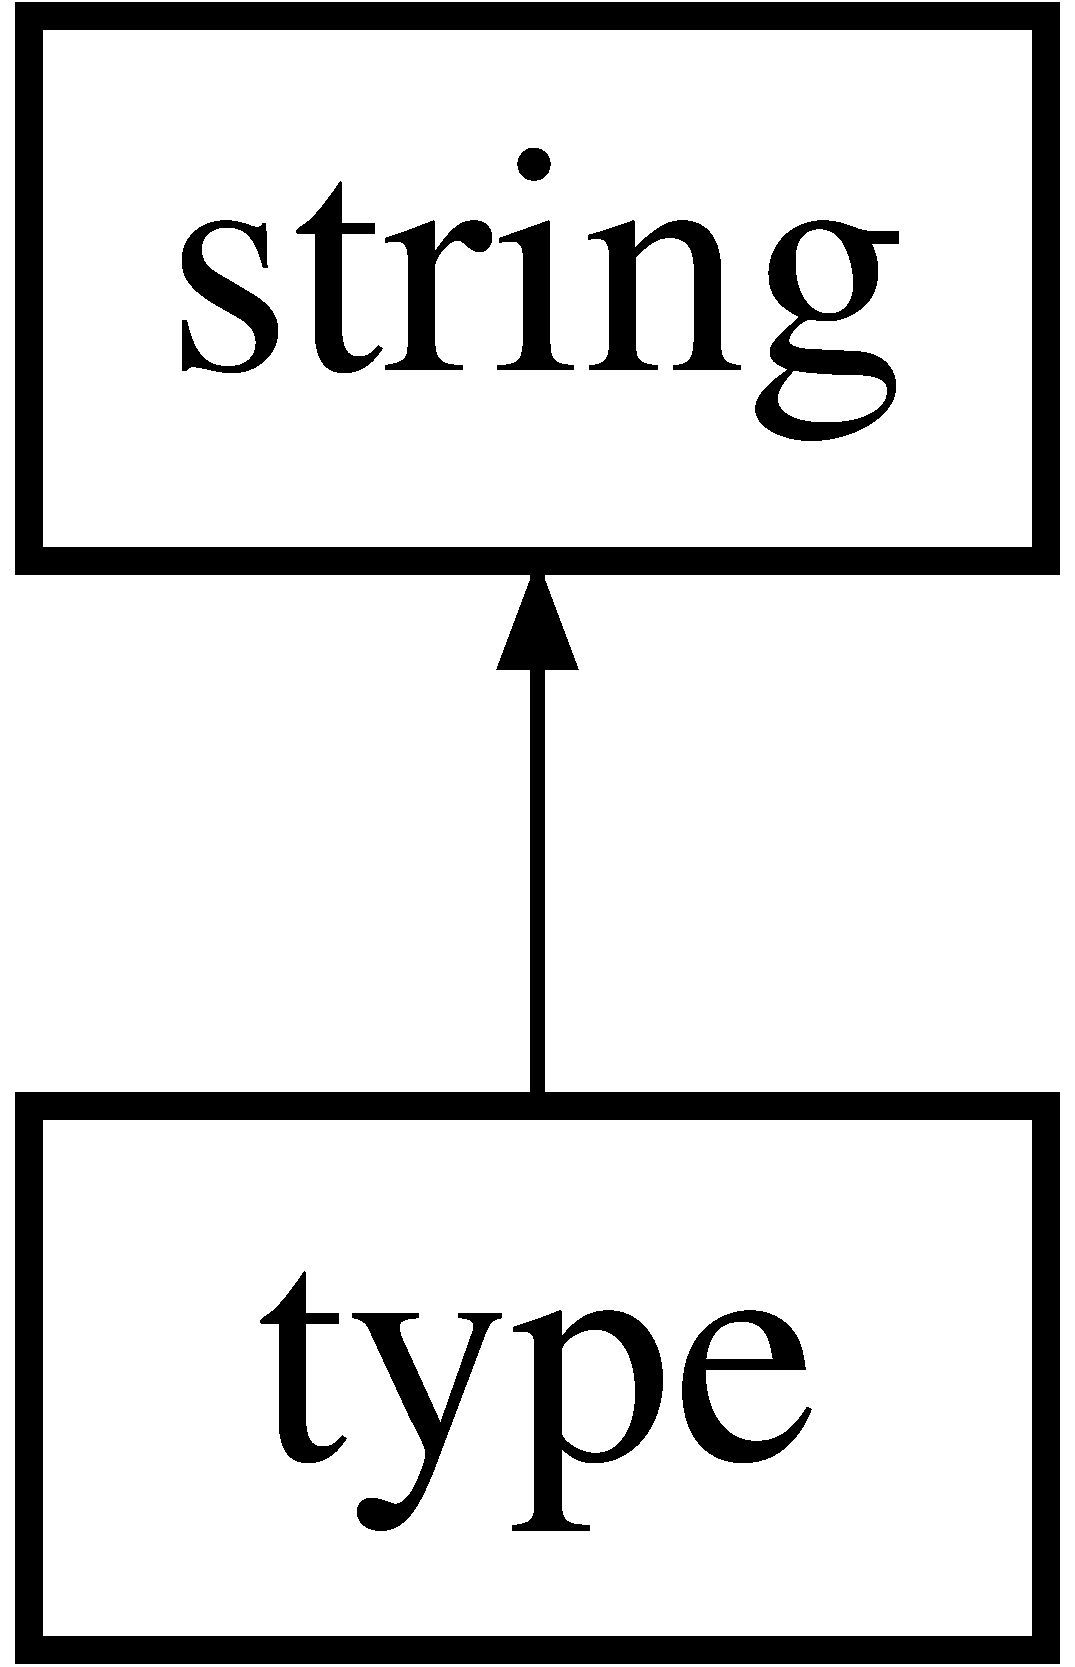
\includegraphics[height=2.000000cm]{classtype}
\end{center}
\end{figure}
\subsection*{Public Types}
\begin{DoxyCompactItemize}
\item 
enum \hyperlink{classtype_a83781d700ce124b4224c316326a5a975}{value} \{ \\*
\hyperlink{classtype_a83781d700ce124b4224c316326a5a975ad559d992c88431b0a1cb90b340929d4e}{Int8}, 
\hyperlink{classtype_a83781d700ce124b4224c316326a5a975a82bbc808c985056ed74b30bcca131fad}{U\+Int8}, 
\hyperlink{classtype_a83781d700ce124b4224c316326a5a975a8d3d044c5da17c4e92e2c61c2f0ea556}{Int16}, 
\hyperlink{classtype_a83781d700ce124b4224c316326a5a975a36b08866238b21675704f38517929e69}{U\+Int16}, 
\\*
\hyperlink{classtype_a83781d700ce124b4224c316326a5a975a62e1ad64aa38ad0b50e1a6bd9b9ae25e}{Int32}, 
\hyperlink{classtype_a83781d700ce124b4224c316326a5a975acfca6c13984dbb7ac515cff88a01826e}{U\+Int32}, 
\hyperlink{classtype_a83781d700ce124b4224c316326a5a975a2cc7bf870db9a3b5e9e580a58b6c1308}{Int64}, 
\hyperlink{classtype_a83781d700ce124b4224c316326a5a975a64538f1914f2fd739bc876253b75fe4c}{U\+Int64}, 
\\*
\hyperlink{classtype_a83781d700ce124b4224c316326a5a975a1b5e448b6fc2bafbc9b5f8e4cc582834}{Float32}, 
\hyperlink{classtype_a83781d700ce124b4224c316326a5a975a72818204734582235e144a1e64563947}{Float64}
 \}
\end{DoxyCompactItemize}
\subsection*{Public Member Functions}
\begin{DoxyCompactItemize}
\item 
\hyperlink{classtype_aed51d13ee609d224084c6cf0a9903f99}{type} (\hyperlink{classtype_a83781d700ce124b4224c316326a5a975}{value} v)
\item 
\hyperlink{classtype_aa5e87da016a56579ba0fc72de17517a5}{type} (const char $\ast$v)
\item 
\hyperlink{classtype_ae83bd8bffd0b7251dd664efe908511e7}{type} (const \+::std\+::string \&v)
\item 
\hyperlink{classtype_a9638b8e282f51d97c9e4e8d703e1f89c}{type} (const \+::\hyperlink{namespacexml__schema_ac0cec83a330f0024e4e318b3deac5104}{xml\+\_\+schema\+::string} \&v)
\item 
\hyperlink{classtype_aae224adcb4348cedbe90f4af5dcf1353}{type} (const \+::xercesc\+::\+D\+O\+M\+Element \&e,\+::\hyperlink{namespacexml__schema_a0612287d030cb2732d31a45b258fdc87}{xml\+\_\+schema\+::flags} f=0,\+::\hyperlink{namespacexml__schema_ada9aa30dc722e93ee2ed7243085402a5}{xml\+\_\+schema\+::container} $\ast$c=0)
\item 
\hyperlink{classtype_a7018bbc02d3c782aed64822b87dda220}{type} (const \+::xercesc\+::\+D\+O\+M\+Attr \&a,\+::\hyperlink{namespacexml__schema_a0612287d030cb2732d31a45b258fdc87}{xml\+\_\+schema\+::flags} f=0,\+::\hyperlink{namespacexml__schema_ada9aa30dc722e93ee2ed7243085402a5}{xml\+\_\+schema\+::container} $\ast$c=0)
\item 
\hyperlink{classtype_ac6751e8c63b52e22f73a1ab24d50a082}{type} (const \+::std\+::string \&s, const \+::xercesc\+::\+D\+O\+M\+Element $\ast$e,\+::\hyperlink{namespacexml__schema_a0612287d030cb2732d31a45b258fdc87}{xml\+\_\+schema\+::flags} f=0,\+::\hyperlink{namespacexml__schema_ada9aa30dc722e93ee2ed7243085402a5}{xml\+\_\+schema\+::container} $\ast$c=0)
\item 
\hyperlink{classtype_aa5eaba8747f76ddbccbb88f68e3311fe}{type} (const \hyperlink{classtype}{type} \&x,\+::\hyperlink{namespacexml__schema_a0612287d030cb2732d31a45b258fdc87}{xml\+\_\+schema\+::flags} f=0,\+::\hyperlink{namespacexml__schema_ada9aa30dc722e93ee2ed7243085402a5}{xml\+\_\+schema\+::container} $\ast$c=0)
\item 
virtual \hyperlink{classtype}{type} $\ast$ \hyperlink{classtype_afebbdc11bbf07de7ab79f148e9cd88b6}{\+\_\+clone} (\+::\hyperlink{namespacexml__schema_a0612287d030cb2732d31a45b258fdc87}{xml\+\_\+schema\+::flags} f=0,\+::\hyperlink{namespacexml__schema_ada9aa30dc722e93ee2ed7243085402a5}{xml\+\_\+schema\+::container} $\ast$c=0) const 
\item 
\hyperlink{classtype}{type} \& \hyperlink{classtype_af55f6d7e02cf92b839d842a58e2911ed}{operator=} (\hyperlink{classtype_a83781d700ce124b4224c316326a5a975}{value} v)
\item 
virtual \hyperlink{classtype_a5bfa60d90029d683cb4e46de45460246}{operator value} () const 
\end{DoxyCompactItemize}
\subsection*{Static Public Attributes}
\begin{DoxyCompactItemize}
\item 
static const char $\ast$const \hyperlink{classtype_a2e3db93564deb68a52e1e54dcb82b41f}{\+\_\+xsd\+\_\+type\+\_\+literals\+\_\+} \mbox{[}10\mbox{]}
\item 
static const \hyperlink{classtype_a83781d700ce124b4224c316326a5a975}{value} \hyperlink{classtype_a847b5fec369eccdbbed240c3a7fcc7a5}{\+\_\+xsd\+\_\+type\+\_\+indexes\+\_\+} \mbox{[}10\mbox{]}
\end{DoxyCompactItemize}
\subsection*{Protected Member Functions}
\begin{DoxyCompactItemize}
\item 
\hyperlink{classtype_a83781d700ce124b4224c316326a5a975}{value} \hyperlink{classtype_ac8957cf4dadb290d74730be2812f4754}{\+\_\+xsd\+\_\+type\+\_\+convert} () const 
\end{DoxyCompactItemize}


\subsection{Member Enumeration Documentation}
\index{type@{type}!value@{value}}
\index{value@{value}!type@{type}}
\subsubsection[{\texorpdfstring{value}{value}}]{\setlength{\rightskip}{0pt plus 5cm}enum {\bf type\+::value}}\hypertarget{classtype_a83781d700ce124b4224c316326a5a975}{}\label{classtype_a83781d700ce124b4224c316326a5a975}
\begin{Desc}
\item[Enumerator]\par
\begin{description}
\index{Int8@{Int8}!type@{type}}\index{type@{type}!Int8@{Int8}}\item[{\em 
Int8\hypertarget{classtype_a83781d700ce124b4224c316326a5a975ad559d992c88431b0a1cb90b340929d4e}{}\label{classtype_a83781d700ce124b4224c316326a5a975ad559d992c88431b0a1cb90b340929d4e}
}]\index{U\+Int8@{U\+Int8}!type@{type}}\index{type@{type}!U\+Int8@{U\+Int8}}\item[{\em 
U\+Int8\hypertarget{classtype_a83781d700ce124b4224c316326a5a975a82bbc808c985056ed74b30bcca131fad}{}\label{classtype_a83781d700ce124b4224c316326a5a975a82bbc808c985056ed74b30bcca131fad}
}]\index{Int16@{Int16}!type@{type}}\index{type@{type}!Int16@{Int16}}\item[{\em 
Int16\hypertarget{classtype_a83781d700ce124b4224c316326a5a975a8d3d044c5da17c4e92e2c61c2f0ea556}{}\label{classtype_a83781d700ce124b4224c316326a5a975a8d3d044c5da17c4e92e2c61c2f0ea556}
}]\index{U\+Int16@{U\+Int16}!type@{type}}\index{type@{type}!U\+Int16@{U\+Int16}}\item[{\em 
U\+Int16\hypertarget{classtype_a83781d700ce124b4224c316326a5a975a36b08866238b21675704f38517929e69}{}\label{classtype_a83781d700ce124b4224c316326a5a975a36b08866238b21675704f38517929e69}
}]\index{Int32@{Int32}!type@{type}}\index{type@{type}!Int32@{Int32}}\item[{\em 
Int32\hypertarget{classtype_a83781d700ce124b4224c316326a5a975a62e1ad64aa38ad0b50e1a6bd9b9ae25e}{}\label{classtype_a83781d700ce124b4224c316326a5a975a62e1ad64aa38ad0b50e1a6bd9b9ae25e}
}]\index{U\+Int32@{U\+Int32}!type@{type}}\index{type@{type}!U\+Int32@{U\+Int32}}\item[{\em 
U\+Int32\hypertarget{classtype_a83781d700ce124b4224c316326a5a975acfca6c13984dbb7ac515cff88a01826e}{}\label{classtype_a83781d700ce124b4224c316326a5a975acfca6c13984dbb7ac515cff88a01826e}
}]\index{Int64@{Int64}!type@{type}}\index{type@{type}!Int64@{Int64}}\item[{\em 
Int64\hypertarget{classtype_a83781d700ce124b4224c316326a5a975a2cc7bf870db9a3b5e9e580a58b6c1308}{}\label{classtype_a83781d700ce124b4224c316326a5a975a2cc7bf870db9a3b5e9e580a58b6c1308}
}]\index{U\+Int64@{U\+Int64}!type@{type}}\index{type@{type}!U\+Int64@{U\+Int64}}\item[{\em 
U\+Int64\hypertarget{classtype_a83781d700ce124b4224c316326a5a975a64538f1914f2fd739bc876253b75fe4c}{}\label{classtype_a83781d700ce124b4224c316326a5a975a64538f1914f2fd739bc876253b75fe4c}
}]\index{Float32@{Float32}!type@{type}}\index{type@{type}!Float32@{Float32}}\item[{\em 
Float32\hypertarget{classtype_a83781d700ce124b4224c316326a5a975a1b5e448b6fc2bafbc9b5f8e4cc582834}{}\label{classtype_a83781d700ce124b4224c316326a5a975a1b5e448b6fc2bafbc9b5f8e4cc582834}
}]\index{Float64@{Float64}!type@{type}}\index{type@{type}!Float64@{Float64}}\item[{\em 
Float64\hypertarget{classtype_a83781d700ce124b4224c316326a5a975a72818204734582235e144a1e64563947}{}\label{classtype_a83781d700ce124b4224c316326a5a975a72818204734582235e144a1e64563947}
}]\end{description}
\end{Desc}


\subsection{Constructor \& Destructor Documentation}
\index{type@{type}!type@{type}}
\index{type@{type}!type@{type}}
\subsubsection[{\texorpdfstring{type(value v)}{type(value v)}}]{\setlength{\rightskip}{0pt plus 5cm}type\+::type (
\begin{DoxyParamCaption}
\item[{{\bf value}}]{v}
\end{DoxyParamCaption}
)}\hypertarget{classtype_aed51d13ee609d224084c6cf0a9903f99}{}\label{classtype_aed51d13ee609d224084c6cf0a9903f99}
\index{type@{type}!type@{type}}
\index{type@{type}!type@{type}}
\subsubsection[{\texorpdfstring{type(const char $\ast$v)}{type(const char *v)}}]{\setlength{\rightskip}{0pt plus 5cm}type\+::type (
\begin{DoxyParamCaption}
\item[{const char $\ast$}]{v}
\end{DoxyParamCaption}
)}\hypertarget{classtype_aa5e87da016a56579ba0fc72de17517a5}{}\label{classtype_aa5e87da016a56579ba0fc72de17517a5}
\index{type@{type}!type@{type}}
\index{type@{type}!type@{type}}
\subsubsection[{\texorpdfstring{type(const \+::std\+::string \&v)}{type(const ::std::string &v)}}]{\setlength{\rightskip}{0pt plus 5cm}type\+::type (
\begin{DoxyParamCaption}
\item[{const \+::std\+::string \&}]{v}
\end{DoxyParamCaption}
)}\hypertarget{classtype_ae83bd8bffd0b7251dd664efe908511e7}{}\label{classtype_ae83bd8bffd0b7251dd664efe908511e7}
\index{type@{type}!type@{type}}
\index{type@{type}!type@{type}}
\subsubsection[{\texorpdfstring{type(const \+::xml\+\_\+schema\+::string \&v)}{type(const ::xml_schema::string &v)}}]{\setlength{\rightskip}{0pt plus 5cm}type\+::type (
\begin{DoxyParamCaption}
\item[{const \+::{\bf xml\+\_\+schema\+::string} \&}]{v}
\end{DoxyParamCaption}
)}\hypertarget{classtype_a9638b8e282f51d97c9e4e8d703e1f89c}{}\label{classtype_a9638b8e282f51d97c9e4e8d703e1f89c}
\index{type@{type}!type@{type}}
\index{type@{type}!type@{type}}
\subsubsection[{\texorpdfstring{type(const \+::xercesc\+::\+D\+O\+M\+Element \&e,\+::xml\+\_\+schema\+::flags f=0,\+::xml\+\_\+schema\+::container $\ast$c=0)}{type(const ::xercesc::DOMElement &e,::xml_schema::flags f=0,::xml_schema::container *c=0)}}]{\setlength{\rightskip}{0pt plus 5cm}type\+::type (
\begin{DoxyParamCaption}
\item[{const \+::xercesc\+::\+D\+O\+M\+Element \&}]{e, }
\item[{\+::{\bf xml\+\_\+schema\+::flags}}]{f = {\ttfamily 0}, }
\item[{\+::{\bf xml\+\_\+schema\+::container} $\ast$}]{c = {\ttfamily 0}}
\end{DoxyParamCaption}
)}\hypertarget{classtype_aae224adcb4348cedbe90f4af5dcf1353}{}\label{classtype_aae224adcb4348cedbe90f4af5dcf1353}
\index{type@{type}!type@{type}}
\index{type@{type}!type@{type}}
\subsubsection[{\texorpdfstring{type(const \+::xercesc\+::\+D\+O\+M\+Attr \&a,\+::xml\+\_\+schema\+::flags f=0,\+::xml\+\_\+schema\+::container $\ast$c=0)}{type(const ::xercesc::DOMAttr &a,::xml_schema::flags f=0,::xml_schema::container *c=0)}}]{\setlength{\rightskip}{0pt plus 5cm}type\+::type (
\begin{DoxyParamCaption}
\item[{const \+::xercesc\+::\+D\+O\+M\+Attr \&}]{a, }
\item[{\+::{\bf xml\+\_\+schema\+::flags}}]{f = {\ttfamily 0}, }
\item[{\+::{\bf xml\+\_\+schema\+::container} $\ast$}]{c = {\ttfamily 0}}
\end{DoxyParamCaption}
)}\hypertarget{classtype_a7018bbc02d3c782aed64822b87dda220}{}\label{classtype_a7018bbc02d3c782aed64822b87dda220}
\index{type@{type}!type@{type}}
\index{type@{type}!type@{type}}
\subsubsection[{\texorpdfstring{type(const \+::std\+::string \&s, const \+::xercesc\+::\+D\+O\+M\+Element $\ast$e,\+::xml\+\_\+schema\+::flags f=0,\+::xml\+\_\+schema\+::container $\ast$c=0)}{type(const ::std::string &s, const ::xercesc::DOMElement *e,::xml_schema::flags f=0,::xml_schema::container *c=0)}}]{\setlength{\rightskip}{0pt plus 5cm}type\+::type (
\begin{DoxyParamCaption}
\item[{const \+::std\+::string \&}]{s, }
\item[{const \+::xercesc\+::\+D\+O\+M\+Element $\ast$}]{e, }
\item[{\+::{\bf xml\+\_\+schema\+::flags}}]{f = {\ttfamily 0}, }
\item[{\+::{\bf xml\+\_\+schema\+::container} $\ast$}]{c = {\ttfamily 0}}
\end{DoxyParamCaption}
)}\hypertarget{classtype_ac6751e8c63b52e22f73a1ab24d50a082}{}\label{classtype_ac6751e8c63b52e22f73a1ab24d50a082}
\index{type@{type}!type@{type}}
\index{type@{type}!type@{type}}
\subsubsection[{\texorpdfstring{type(const type \&x,\+::xml\+\_\+schema\+::flags f=0,\+::xml\+\_\+schema\+::container $\ast$c=0)}{type(const type &x,::xml_schema::flags f=0,::xml_schema::container *c=0)}}]{\setlength{\rightskip}{0pt plus 5cm}type\+::type (
\begin{DoxyParamCaption}
\item[{const {\bf type} \&}]{x, }
\item[{\+::{\bf xml\+\_\+schema\+::flags}}]{f = {\ttfamily 0}, }
\item[{\+::{\bf xml\+\_\+schema\+::container} $\ast$}]{c = {\ttfamily 0}}
\end{DoxyParamCaption}
)}\hypertarget{classtype_aa5eaba8747f76ddbccbb88f68e3311fe}{}\label{classtype_aa5eaba8747f76ddbccbb88f68e3311fe}


\subsection{Member Function Documentation}
\index{type@{type}!\+\_\+clone@{\+\_\+clone}}
\index{\+\_\+clone@{\+\_\+clone}!type@{type}}
\subsubsection[{\texorpdfstring{\+\_\+clone(\+::xml\+\_\+schema\+::flags f=0,\+::xml\+\_\+schema\+::container $\ast$c=0) const }{_clone(::xml_schema::flags f=0,::xml_schema::container *c=0) const }}]{\setlength{\rightskip}{0pt plus 5cm}{\bf type} $\ast$ type\+::\+\_\+clone (
\begin{DoxyParamCaption}
\item[{\+::{\bf xml\+\_\+schema\+::flags}}]{f = {\ttfamily 0}, }
\item[{\+::{\bf xml\+\_\+schema\+::container} $\ast$}]{c = {\ttfamily 0}}
\end{DoxyParamCaption}
) const\hspace{0.3cm}{\ttfamily [virtual]}}\hypertarget{classtype_afebbdc11bbf07de7ab79f148e9cd88b6}{}\label{classtype_afebbdc11bbf07de7ab79f148e9cd88b6}
\index{type@{type}!\+\_\+xsd\+\_\+type\+\_\+convert@{\+\_\+xsd\+\_\+type\+\_\+convert}}
\index{\+\_\+xsd\+\_\+type\+\_\+convert@{\+\_\+xsd\+\_\+type\+\_\+convert}!type@{type}}
\subsubsection[{\texorpdfstring{\+\_\+xsd\+\_\+type\+\_\+convert() const }{_xsd_type_convert() const }}]{\setlength{\rightskip}{0pt plus 5cm}{\bf type\+::value} type\+::\+\_\+xsd\+\_\+type\+\_\+convert (
\begin{DoxyParamCaption}
{}
\end{DoxyParamCaption}
) const\hspace{0.3cm}{\ttfamily [protected]}}\hypertarget{classtype_ac8957cf4dadb290d74730be2812f4754}{}\label{classtype_ac8957cf4dadb290d74730be2812f4754}
\index{type@{type}!operator value@{operator value}}
\index{operator value@{operator value}!type@{type}}
\subsubsection[{\texorpdfstring{operator value() const }{operator value() const }}]{\setlength{\rightskip}{0pt plus 5cm}virtual type\+::operator {\bf value} (
\begin{DoxyParamCaption}
{}
\end{DoxyParamCaption}
) const\hspace{0.3cm}{\ttfamily [inline]}, {\ttfamily [virtual]}}\hypertarget{classtype_a5bfa60d90029d683cb4e46de45460246}{}\label{classtype_a5bfa60d90029d683cb4e46de45460246}
\index{type@{type}!operator=@{operator=}}
\index{operator=@{operator=}!type@{type}}
\subsubsection[{\texorpdfstring{operator=(value v)}{operator=(value v)}}]{\setlength{\rightskip}{0pt plus 5cm}{\bf type} \& type\+::operator= (
\begin{DoxyParamCaption}
\item[{{\bf value}}]{v}
\end{DoxyParamCaption}
)}\hypertarget{classtype_af55f6d7e02cf92b839d842a58e2911ed}{}\label{classtype_af55f6d7e02cf92b839d842a58e2911ed}


\subsection{Member Data Documentation}
\index{type@{type}!\+\_\+xsd\+\_\+type\+\_\+indexes\+\_\+@{\+\_\+xsd\+\_\+type\+\_\+indexes\+\_\+}}
\index{\+\_\+xsd\+\_\+type\+\_\+indexes\+\_\+@{\+\_\+xsd\+\_\+type\+\_\+indexes\+\_\+}!type@{type}}
\subsubsection[{\texorpdfstring{\+\_\+xsd\+\_\+type\+\_\+indexes\+\_\+}{_xsd_type_indexes_}}]{\setlength{\rightskip}{0pt plus 5cm}const {\bf type\+::value} type\+::\+\_\+xsd\+\_\+type\+\_\+indexes\+\_\+\hspace{0.3cm}{\ttfamily [static]}}\hypertarget{classtype_a847b5fec369eccdbbed240c3a7fcc7a5}{}\label{classtype_a847b5fec369eccdbbed240c3a7fcc7a5}
{\bfseries Initial value\+:}
\begin{DoxyCode}
=
\{
  \hyperlink{classtype_a83781d700ce124b4224c316326a5a975a1b5e448b6fc2bafbc9b5f8e4cc582834}{::type::Float32},
  \hyperlink{classtype_a83781d700ce124b4224c316326a5a975a72818204734582235e144a1e64563947}{::type::Float64},
  \hyperlink{classtype_a83781d700ce124b4224c316326a5a975a8d3d044c5da17c4e92e2c61c2f0ea556}{::type::Int16},
  \hyperlink{classtype_a83781d700ce124b4224c316326a5a975a62e1ad64aa38ad0b50e1a6bd9b9ae25e}{::type::Int32},
  \hyperlink{classtype_a83781d700ce124b4224c316326a5a975a2cc7bf870db9a3b5e9e580a58b6c1308}{::type::Int64},
  \hyperlink{classtype_a83781d700ce124b4224c316326a5a975ad559d992c88431b0a1cb90b340929d4e}{::type::Int8},
  \hyperlink{classtype_a83781d700ce124b4224c316326a5a975a36b08866238b21675704f38517929e69}{::type::UInt16},
  \hyperlink{classtype_a83781d700ce124b4224c316326a5a975acfca6c13984dbb7ac515cff88a01826e}{::type::UInt32},
  \hyperlink{classtype_a83781d700ce124b4224c316326a5a975a64538f1914f2fd739bc876253b75fe4c}{::type::UInt64},
  \hyperlink{classtype_a83781d700ce124b4224c316326a5a975a82bbc808c985056ed74b30bcca131fad}{::type::UInt8}
\}
\end{DoxyCode}
\index{type@{type}!\+\_\+xsd\+\_\+type\+\_\+literals\+\_\+@{\+\_\+xsd\+\_\+type\+\_\+literals\+\_\+}}
\index{\+\_\+xsd\+\_\+type\+\_\+literals\+\_\+@{\+\_\+xsd\+\_\+type\+\_\+literals\+\_\+}!type@{type}}
\subsubsection[{\texorpdfstring{\+\_\+xsd\+\_\+type\+\_\+literals\+\_\+}{_xsd_type_literals_}}]{\setlength{\rightskip}{0pt plus 5cm}const char $\ast$const type\+::\+\_\+xsd\+\_\+type\+\_\+literals\+\_\+\hspace{0.3cm}{\ttfamily [static]}}\hypertarget{classtype_a2e3db93564deb68a52e1e54dcb82b41f}{}\label{classtype_a2e3db93564deb68a52e1e54dcb82b41f}
{\bfseries Initial value\+:}
\begin{DoxyCode}
=
\{
  \textcolor{stringliteral}{"Int8"},
  \textcolor{stringliteral}{"UInt8"},
  \textcolor{stringliteral}{"Int16"},
  \textcolor{stringliteral}{"UInt16"},
  \textcolor{stringliteral}{"Int32"},
  \textcolor{stringliteral}{"UInt32"},
  \textcolor{stringliteral}{"Int64"},
  \textcolor{stringliteral}{"UInt64"},
  \textcolor{stringliteral}{"Float32"},
  \textcolor{stringliteral}{"Float64"}
\}
\end{DoxyCode}


The documentation for this class was generated from the following files\+:\begin{DoxyCompactItemize}
\item 
src/output\+Writer/\hyperlink{vtk-unstructured_8h}{vtk-\/unstructured.\+h}\item 
src/output\+Writer/\hyperlink{vtk-unstructured_8cpp}{vtk-\/unstructured.\+cpp}\end{DoxyCompactItemize}

\hypertarget{classUnstructuredGrid__t}{}\section{Unstructured\+Grid\+\_\+t Class Reference}
\label{classUnstructuredGrid__t}\index{Unstructured\+Grid\+\_\+t@{Unstructured\+Grid\+\_\+t}}


{\ttfamily \#include $<$vtk-\/unstructured.\+h$>$}

Inheritance diagram for Unstructured\+Grid\+\_\+t\+:\begin{figure}[H]
\begin{center}
\leavevmode
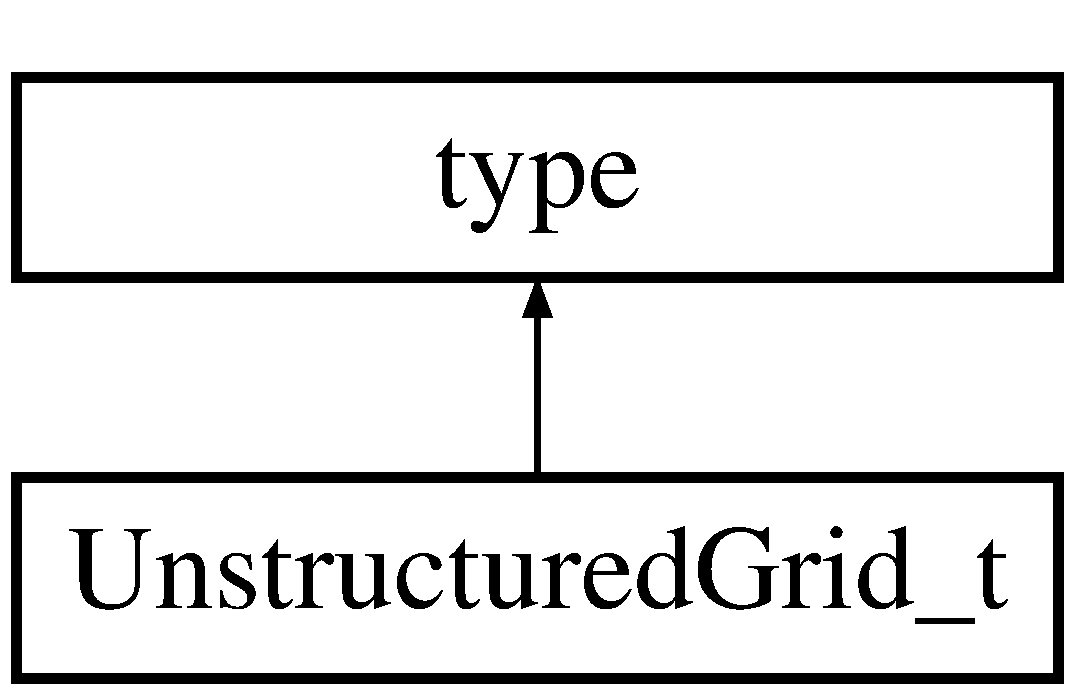
\includegraphics[height=2.000000cm]{classUnstructuredGrid__t}
\end{center}
\end{figure}
\subsection*{Public Types}
\begin{DoxyCompactItemize}
\item 
typedef \+::\hyperlink{classPieceUnstructuredGrid__t}{Piece\+Unstructured\+Grid\+\_\+t} \hyperlink{classUnstructuredGrid__t_a559913611314b34f4868027fc91e35bc}{Piece\+\_\+type}
\item 
typedef \+::xsd\+::cxx\+::tree\+::traits$<$ \hyperlink{classUnstructuredGrid__t_a559913611314b34f4868027fc91e35bc}{Piece\+\_\+type}, char $>$ \hyperlink{classUnstructuredGrid__t_a8a9bf012c364a5fbb78aac9a319a4dad}{Piece\+\_\+traits}
\end{DoxyCompactItemize}
\subsection*{Public Member Functions}
\begin{DoxyCompactItemize}
\item 
const \hyperlink{classUnstructuredGrid__t_a559913611314b34f4868027fc91e35bc}{Piece\+\_\+type} \& \hyperlink{classUnstructuredGrid__t_a32fdd47d79cfdd2eb071cf674b7cc9ee}{Piece} () const 
\item 
\hyperlink{classUnstructuredGrid__t_a559913611314b34f4868027fc91e35bc}{Piece\+\_\+type} \& \hyperlink{classUnstructuredGrid__t_a66b7c6fc204fdc78b4611fd132771573}{Piece} ()
\item 
void \hyperlink{classUnstructuredGrid__t_a97ef3f79738631a4265c4fbeb170f04d}{Piece} (const \hyperlink{classUnstructuredGrid__t_a559913611314b34f4868027fc91e35bc}{Piece\+\_\+type} \&x)
\item 
void \hyperlink{classUnstructuredGrid__t_ab6746290ddee77043f5830b05d750972}{Piece} (\+::std\+::unique\+\_\+ptr$<$ \hyperlink{classUnstructuredGrid__t_a559913611314b34f4868027fc91e35bc}{Piece\+\_\+type} $>$ p)
\item 
\hyperlink{classUnstructuredGrid__t_a00bf6957ea7e3313e2890bd4c02f8981}{Unstructured\+Grid\+\_\+t} (const \hyperlink{classUnstructuredGrid__t_a559913611314b34f4868027fc91e35bc}{Piece\+\_\+type} \&)
\item 
\hyperlink{classUnstructuredGrid__t_a5335359377e3026191868e93675a5436}{Unstructured\+Grid\+\_\+t} (\+::std\+::unique\+\_\+ptr$<$ \hyperlink{classUnstructuredGrid__t_a559913611314b34f4868027fc91e35bc}{Piece\+\_\+type} $>$)
\item 
\hyperlink{classUnstructuredGrid__t_ad6fb3d97ad8d9443d53e1152a9fa6004}{Unstructured\+Grid\+\_\+t} (const \+::xercesc\+::\+D\+O\+M\+Element \&e,\+::\hyperlink{namespacexml__schema_a0612287d030cb2732d31a45b258fdc87}{xml\+\_\+schema\+::flags} f=0,\+::\hyperlink{namespacexml__schema_ada9aa30dc722e93ee2ed7243085402a5}{xml\+\_\+schema\+::container} $\ast$c=0)
\item 
\hyperlink{classUnstructuredGrid__t_a893b6debad8369f36a3cdc2aaa22b478}{Unstructured\+Grid\+\_\+t} (const \hyperlink{classUnstructuredGrid__t}{Unstructured\+Grid\+\_\+t} \&x,\+::\hyperlink{namespacexml__schema_a0612287d030cb2732d31a45b258fdc87}{xml\+\_\+schema\+::flags} f=0,\+::\hyperlink{namespacexml__schema_ada9aa30dc722e93ee2ed7243085402a5}{xml\+\_\+schema\+::container} $\ast$c=0)
\item 
virtual \hyperlink{classUnstructuredGrid__t}{Unstructured\+Grid\+\_\+t} $\ast$ \hyperlink{classUnstructuredGrid__t_ae51f374b8650e990f30723bdcf181f2d}{\+\_\+clone} (\+::\hyperlink{namespacexml__schema_a0612287d030cb2732d31a45b258fdc87}{xml\+\_\+schema\+::flags} f=0,\+::\hyperlink{namespacexml__schema_ada9aa30dc722e93ee2ed7243085402a5}{xml\+\_\+schema\+::container} $\ast$c=0) const 
\item 
\hyperlink{classUnstructuredGrid__t}{Unstructured\+Grid\+\_\+t} \& \hyperlink{classUnstructuredGrid__t_ac33ad0177719bcab9caa4fdf0efc51ae}{operator=} (const \hyperlink{classUnstructuredGrid__t}{Unstructured\+Grid\+\_\+t} \&x)
\item 
virtual \hyperlink{classUnstructuredGrid__t_a6fb9239ab1215edd7e7822a66d3af53c}{$\sim$\+Unstructured\+Grid\+\_\+t} ()
\end{DoxyCompactItemize}
\subsection*{Protected Member Functions}
\begin{DoxyCompactItemize}
\item 
void \hyperlink{classUnstructuredGrid__t_ae0663e380fcfcfd8b663a0a52241c034}{parse} (\+::xsd\+::cxx\+::xml\+::dom\+::parser$<$ char $>$ \&,\+::\hyperlink{namespacexml__schema_a0612287d030cb2732d31a45b258fdc87}{xml\+\_\+schema\+::flags})
\end{DoxyCompactItemize}
\subsection*{Protected Attributes}
\begin{DoxyCompactItemize}
\item 
\+::xsd\+::cxx\+::tree\+::one$<$ \hyperlink{classUnstructuredGrid__t_a559913611314b34f4868027fc91e35bc}{Piece\+\_\+type} $>$ \hyperlink{classUnstructuredGrid__t_aec675f4635fe96f8e4e5964e8220e0a0}{Piece\+\_\+}
\end{DoxyCompactItemize}


\subsection{Member Typedef Documentation}
\index{Unstructured\+Grid\+\_\+t@{Unstructured\+Grid\+\_\+t}!Piece\+\_\+traits@{Piece\+\_\+traits}}
\index{Piece\+\_\+traits@{Piece\+\_\+traits}!Unstructured\+Grid\+\_\+t@{Unstructured\+Grid\+\_\+t}}
\subsubsection[{\texorpdfstring{Piece\+\_\+traits}{Piece_traits}}]{\setlength{\rightskip}{0pt plus 5cm}typedef \+::xsd\+::cxx\+::tree\+::traits$<$ {\bf Piece\+\_\+type}, char $>$ {\bf Unstructured\+Grid\+\_\+t\+::\+Piece\+\_\+traits}}\hypertarget{classUnstructuredGrid__t_a8a9bf012c364a5fbb78aac9a319a4dad}{}\label{classUnstructuredGrid__t_a8a9bf012c364a5fbb78aac9a319a4dad}
\index{Unstructured\+Grid\+\_\+t@{Unstructured\+Grid\+\_\+t}!Piece\+\_\+type@{Piece\+\_\+type}}
\index{Piece\+\_\+type@{Piece\+\_\+type}!Unstructured\+Grid\+\_\+t@{Unstructured\+Grid\+\_\+t}}
\subsubsection[{\texorpdfstring{Piece\+\_\+type}{Piece_type}}]{\setlength{\rightskip}{0pt plus 5cm}typedef \+::{\bf Piece\+Unstructured\+Grid\+\_\+t} {\bf Unstructured\+Grid\+\_\+t\+::\+Piece\+\_\+type}}\hypertarget{classUnstructuredGrid__t_a559913611314b34f4868027fc91e35bc}{}\label{classUnstructuredGrid__t_a559913611314b34f4868027fc91e35bc}


\subsection{Constructor \& Destructor Documentation}
\index{Unstructured\+Grid\+\_\+t@{Unstructured\+Grid\+\_\+t}!Unstructured\+Grid\+\_\+t@{Unstructured\+Grid\+\_\+t}}
\index{Unstructured\+Grid\+\_\+t@{Unstructured\+Grid\+\_\+t}!Unstructured\+Grid\+\_\+t@{Unstructured\+Grid\+\_\+t}}
\subsubsection[{\texorpdfstring{Unstructured\+Grid\+\_\+t(const Piece\+\_\+type \&)}{UnstructuredGrid_t(const Piece_type &)}}]{\setlength{\rightskip}{0pt plus 5cm}Unstructured\+Grid\+\_\+t\+::\+Unstructured\+Grid\+\_\+t (
\begin{DoxyParamCaption}
\item[{const {\bf Piece\+\_\+type} \&}]{Piece}
\end{DoxyParamCaption}
)}\hypertarget{classUnstructuredGrid__t_a00bf6957ea7e3313e2890bd4c02f8981}{}\label{classUnstructuredGrid__t_a00bf6957ea7e3313e2890bd4c02f8981}
\index{Unstructured\+Grid\+\_\+t@{Unstructured\+Grid\+\_\+t}!Unstructured\+Grid\+\_\+t@{Unstructured\+Grid\+\_\+t}}
\index{Unstructured\+Grid\+\_\+t@{Unstructured\+Grid\+\_\+t}!Unstructured\+Grid\+\_\+t@{Unstructured\+Grid\+\_\+t}}
\subsubsection[{\texorpdfstring{Unstructured\+Grid\+\_\+t(\+::std\+::unique\+\_\+ptr$<$ Piece\+\_\+type $>$)}{UnstructuredGrid_t(::std::unique_ptr< Piece_type >)}}]{\setlength{\rightskip}{0pt plus 5cm}Unstructured\+Grid\+\_\+t\+::\+Unstructured\+Grid\+\_\+t (
\begin{DoxyParamCaption}
\item[{\+::std\+::unique\+\_\+ptr$<$ {\bf Piece\+\_\+type} $>$}]{Piece}
\end{DoxyParamCaption}
)}\hypertarget{classUnstructuredGrid__t_a5335359377e3026191868e93675a5436}{}\label{classUnstructuredGrid__t_a5335359377e3026191868e93675a5436}
\index{Unstructured\+Grid\+\_\+t@{Unstructured\+Grid\+\_\+t}!Unstructured\+Grid\+\_\+t@{Unstructured\+Grid\+\_\+t}}
\index{Unstructured\+Grid\+\_\+t@{Unstructured\+Grid\+\_\+t}!Unstructured\+Grid\+\_\+t@{Unstructured\+Grid\+\_\+t}}
\subsubsection[{\texorpdfstring{Unstructured\+Grid\+\_\+t(const \+::xercesc\+::\+D\+O\+M\+Element \&e,\+::xml\+\_\+schema\+::flags f=0,\+::xml\+\_\+schema\+::container $\ast$c=0)}{UnstructuredGrid_t(const ::xercesc::DOMElement &e,::xml_schema::flags f=0,::xml_schema::container *c=0)}}]{\setlength{\rightskip}{0pt plus 5cm}Unstructured\+Grid\+\_\+t\+::\+Unstructured\+Grid\+\_\+t (
\begin{DoxyParamCaption}
\item[{const \+::xercesc\+::\+D\+O\+M\+Element \&}]{e, }
\item[{\+::{\bf xml\+\_\+schema\+::flags}}]{f = {\ttfamily 0}, }
\item[{\+::{\bf xml\+\_\+schema\+::container} $\ast$}]{c = {\ttfamily 0}}
\end{DoxyParamCaption}
)}\hypertarget{classUnstructuredGrid__t_ad6fb3d97ad8d9443d53e1152a9fa6004}{}\label{classUnstructuredGrid__t_ad6fb3d97ad8d9443d53e1152a9fa6004}
\index{Unstructured\+Grid\+\_\+t@{Unstructured\+Grid\+\_\+t}!Unstructured\+Grid\+\_\+t@{Unstructured\+Grid\+\_\+t}}
\index{Unstructured\+Grid\+\_\+t@{Unstructured\+Grid\+\_\+t}!Unstructured\+Grid\+\_\+t@{Unstructured\+Grid\+\_\+t}}
\subsubsection[{\texorpdfstring{Unstructured\+Grid\+\_\+t(const Unstructured\+Grid\+\_\+t \&x,\+::xml\+\_\+schema\+::flags f=0,\+::xml\+\_\+schema\+::container $\ast$c=0)}{UnstructuredGrid_t(const UnstructuredGrid_t &x,::xml_schema::flags f=0,::xml_schema::container *c=0)}}]{\setlength{\rightskip}{0pt plus 5cm}Unstructured\+Grid\+\_\+t\+::\+Unstructured\+Grid\+\_\+t (
\begin{DoxyParamCaption}
\item[{const {\bf Unstructured\+Grid\+\_\+t} \&}]{x, }
\item[{\+::{\bf xml\+\_\+schema\+::flags}}]{f = {\ttfamily 0}, }
\item[{\+::{\bf xml\+\_\+schema\+::container} $\ast$}]{c = {\ttfamily 0}}
\end{DoxyParamCaption}
)}\hypertarget{classUnstructuredGrid__t_a893b6debad8369f36a3cdc2aaa22b478}{}\label{classUnstructuredGrid__t_a893b6debad8369f36a3cdc2aaa22b478}
\index{Unstructured\+Grid\+\_\+t@{Unstructured\+Grid\+\_\+t}!````~Unstructured\+Grid\+\_\+t@{$\sim$\+Unstructured\+Grid\+\_\+t}}
\index{````~Unstructured\+Grid\+\_\+t@{$\sim$\+Unstructured\+Grid\+\_\+t}!Unstructured\+Grid\+\_\+t@{Unstructured\+Grid\+\_\+t}}
\subsubsection[{\texorpdfstring{$\sim$\+Unstructured\+Grid\+\_\+t()}{~UnstructuredGrid_t()}}]{\setlength{\rightskip}{0pt plus 5cm}Unstructured\+Grid\+\_\+t\+::$\sim$\+Unstructured\+Grid\+\_\+t (
\begin{DoxyParamCaption}
{}
\end{DoxyParamCaption}
)\hspace{0.3cm}{\ttfamily [virtual]}}\hypertarget{classUnstructuredGrid__t_a6fb9239ab1215edd7e7822a66d3af53c}{}\label{classUnstructuredGrid__t_a6fb9239ab1215edd7e7822a66d3af53c}


\subsection{Member Function Documentation}
\index{Unstructured\+Grid\+\_\+t@{Unstructured\+Grid\+\_\+t}!\+\_\+clone@{\+\_\+clone}}
\index{\+\_\+clone@{\+\_\+clone}!Unstructured\+Grid\+\_\+t@{Unstructured\+Grid\+\_\+t}}
\subsubsection[{\texorpdfstring{\+\_\+clone(\+::xml\+\_\+schema\+::flags f=0,\+::xml\+\_\+schema\+::container $\ast$c=0) const }{_clone(::xml_schema::flags f=0,::xml_schema::container *c=0) const }}]{\setlength{\rightskip}{0pt plus 5cm}{\bf Unstructured\+Grid\+\_\+t} $\ast$ Unstructured\+Grid\+\_\+t\+::\+\_\+clone (
\begin{DoxyParamCaption}
\item[{\+::{\bf xml\+\_\+schema\+::flags}}]{f = {\ttfamily 0}, }
\item[{\+::{\bf xml\+\_\+schema\+::container} $\ast$}]{c = {\ttfamily 0}}
\end{DoxyParamCaption}
) const\hspace{0.3cm}{\ttfamily [virtual]}}\hypertarget{classUnstructuredGrid__t_ae51f374b8650e990f30723bdcf181f2d}{}\label{classUnstructuredGrid__t_ae51f374b8650e990f30723bdcf181f2d}
\index{Unstructured\+Grid\+\_\+t@{Unstructured\+Grid\+\_\+t}!operator=@{operator=}}
\index{operator=@{operator=}!Unstructured\+Grid\+\_\+t@{Unstructured\+Grid\+\_\+t}}
\subsubsection[{\texorpdfstring{operator=(const Unstructured\+Grid\+\_\+t \&x)}{operator=(const UnstructuredGrid_t &x)}}]{\setlength{\rightskip}{0pt plus 5cm}{\bf Unstructured\+Grid\+\_\+t} \& Unstructured\+Grid\+\_\+t\+::operator= (
\begin{DoxyParamCaption}
\item[{const {\bf Unstructured\+Grid\+\_\+t} \&}]{x}
\end{DoxyParamCaption}
)}\hypertarget{classUnstructuredGrid__t_ac33ad0177719bcab9caa4fdf0efc51ae}{}\label{classUnstructuredGrid__t_ac33ad0177719bcab9caa4fdf0efc51ae}
\index{Unstructured\+Grid\+\_\+t@{Unstructured\+Grid\+\_\+t}!parse@{parse}}
\index{parse@{parse}!Unstructured\+Grid\+\_\+t@{Unstructured\+Grid\+\_\+t}}
\subsubsection[{\texorpdfstring{parse(\+::xsd\+::cxx\+::xml\+::dom\+::parser$<$ char $>$ \&,\+::xml\+\_\+schema\+::flags)}{parse(::xsd::cxx::xml::dom::parser< char > &,::xml_schema::flags)}}]{\setlength{\rightskip}{0pt plus 5cm}void Unstructured\+Grid\+\_\+t\+::parse (
\begin{DoxyParamCaption}
\item[{\+::xsd\+::cxx\+::xml\+::dom\+::parser$<$ char $>$ \&}]{p, }
\item[{\+::{\bf xml\+\_\+schema\+::flags}}]{f}
\end{DoxyParamCaption}
)\hspace{0.3cm}{\ttfamily [protected]}}\hypertarget{classUnstructuredGrid__t_ae0663e380fcfcfd8b663a0a52241c034}{}\label{classUnstructuredGrid__t_ae0663e380fcfcfd8b663a0a52241c034}
\index{Unstructured\+Grid\+\_\+t@{Unstructured\+Grid\+\_\+t}!Piece@{Piece}}
\index{Piece@{Piece}!Unstructured\+Grid\+\_\+t@{Unstructured\+Grid\+\_\+t}}
\subsubsection[{\texorpdfstring{Piece() const }{Piece() const }}]{\setlength{\rightskip}{0pt plus 5cm}const {\bf Unstructured\+Grid\+\_\+t\+::\+Piece\+\_\+type} \& Unstructured\+Grid\+\_\+t\+::\+Piece (
\begin{DoxyParamCaption}
{}
\end{DoxyParamCaption}
) const}\hypertarget{classUnstructuredGrid__t_a32fdd47d79cfdd2eb071cf674b7cc9ee}{}\label{classUnstructuredGrid__t_a32fdd47d79cfdd2eb071cf674b7cc9ee}
\index{Unstructured\+Grid\+\_\+t@{Unstructured\+Grid\+\_\+t}!Piece@{Piece}}
\index{Piece@{Piece}!Unstructured\+Grid\+\_\+t@{Unstructured\+Grid\+\_\+t}}
\subsubsection[{\texorpdfstring{Piece()}{Piece()}}]{\setlength{\rightskip}{0pt plus 5cm}{\bf Unstructured\+Grid\+\_\+t\+::\+Piece\+\_\+type} \& Unstructured\+Grid\+\_\+t\+::\+Piece (
\begin{DoxyParamCaption}
{}
\end{DoxyParamCaption}
)}\hypertarget{classUnstructuredGrid__t_a66b7c6fc204fdc78b4611fd132771573}{}\label{classUnstructuredGrid__t_a66b7c6fc204fdc78b4611fd132771573}
\index{Unstructured\+Grid\+\_\+t@{Unstructured\+Grid\+\_\+t}!Piece@{Piece}}
\index{Piece@{Piece}!Unstructured\+Grid\+\_\+t@{Unstructured\+Grid\+\_\+t}}
\subsubsection[{\texorpdfstring{Piece(const Piece\+\_\+type \&x)}{Piece(const Piece_type &x)}}]{\setlength{\rightskip}{0pt plus 5cm}void Unstructured\+Grid\+\_\+t\+::\+Piece (
\begin{DoxyParamCaption}
\item[{const {\bf Piece\+\_\+type} \&}]{x}
\end{DoxyParamCaption}
)}\hypertarget{classUnstructuredGrid__t_a97ef3f79738631a4265c4fbeb170f04d}{}\label{classUnstructuredGrid__t_a97ef3f79738631a4265c4fbeb170f04d}
\index{Unstructured\+Grid\+\_\+t@{Unstructured\+Grid\+\_\+t}!Piece@{Piece}}
\index{Piece@{Piece}!Unstructured\+Grid\+\_\+t@{Unstructured\+Grid\+\_\+t}}
\subsubsection[{\texorpdfstring{Piece(\+::std\+::unique\+\_\+ptr$<$ Piece\+\_\+type $>$ p)}{Piece(::std::unique_ptr< Piece_type > p)}}]{\setlength{\rightskip}{0pt plus 5cm}void Unstructured\+Grid\+\_\+t\+::\+Piece (
\begin{DoxyParamCaption}
\item[{\+::std\+::unique\+\_\+ptr$<$ {\bf Piece\+\_\+type} $>$}]{p}
\end{DoxyParamCaption}
)}\hypertarget{classUnstructuredGrid__t_ab6746290ddee77043f5830b05d750972}{}\label{classUnstructuredGrid__t_ab6746290ddee77043f5830b05d750972}


\subsection{Member Data Documentation}
\index{Unstructured\+Grid\+\_\+t@{Unstructured\+Grid\+\_\+t}!Piece\+\_\+@{Piece\+\_\+}}
\index{Piece\+\_\+@{Piece\+\_\+}!Unstructured\+Grid\+\_\+t@{Unstructured\+Grid\+\_\+t}}
\subsubsection[{\texorpdfstring{Piece\+\_\+}{Piece_}}]{\setlength{\rightskip}{0pt plus 5cm}\+::xsd\+::cxx\+::tree\+::one$<$ {\bf Piece\+\_\+type} $>$ Unstructured\+Grid\+\_\+t\+::\+Piece\+\_\+\hspace{0.3cm}{\ttfamily [protected]}}\hypertarget{classUnstructuredGrid__t_aec675f4635fe96f8e4e5964e8220e0a0}{}\label{classUnstructuredGrid__t_aec675f4635fe96f8e4e5964e8220e0a0}


The documentation for this class was generated from the following files\+:\begin{DoxyCompactItemize}
\item 
src/output\+Writer/\hyperlink{vtk-unstructured_8h}{vtk-\/unstructured.\+h}\item 
src/output\+Writer/\hyperlink{vtk-unstructured_8cpp}{vtk-\/unstructured.\+cpp}\end{DoxyCompactItemize}

\hypertarget{classutils_1_1Vector}{}\section{utils\+:\+:Vector$<$ type, length $>$ Class Template Reference}
\label{classutils_1_1Vector}\index{utils\+::\+Vector$<$ type, length $>$@{utils\+::\+Vector$<$ type, length $>$}}


{\ttfamily \#include $<$Vector.\+h$>$}

\subsection*{Public Member Functions}
\begin{DoxyCompactItemize}
\item 
\hyperlink{classutils_1_1Vector_a71b42b489a54eb7eae82cff54fae0e12}{Vector} ()
\item 
\hyperlink{classutils_1_1Vector_a5f7d3385f6db28e1376d16e46f1a485f}{Vector} (\hyperlink{classtype}{type} arg)
\item 
\hyperlink{classutils_1_1Vector_a61a6f07c23829b70273ab4578bbb2332}{Vector} (\hyperlink{classtype}{type} args\mbox{[}length\mbox{]})
\item 
\hyperlink{classutils_1_1Vector_abb684db142444c4b19e6cd854db1a0d8}{Vector} (const \hyperlink{classutils_1_1Vector}{Vector} \&other)
\item 
\hyperlink{classutils_1_1Vector}{Vector} \hyperlink{classutils_1_1Vector_aeb0edeaa6b74a48839892e16623b0949}{operator+} (const \hyperlink{classutils_1_1Vector}{Vector} \&rhs) const 
\item 
\hyperlink{classutils_1_1Vector}{Vector} \& \hyperlink{classutils_1_1Vector_aa98dd61c4277e7e203292fcda5e68a69}{operator+=} (const \hyperlink{classutils_1_1Vector}{Vector} \&rhs)
\item 
\hyperlink{classutils_1_1Vector}{Vector} \hyperlink{classutils_1_1Vector_ad6e42a80810a58993f39e1d876eb5716}{operator-\/} (const \hyperlink{classutils_1_1Vector}{Vector} \&rhs) const 
\item 
\hyperlink{classutils_1_1Vector}{Vector} \& \hyperlink{classutils_1_1Vector_abe90a3569989271093c64363707d9cad}{operator-\/=} (const \hyperlink{classutils_1_1Vector}{Vector} \&rhs)
\item 
\hyperlink{classutils_1_1Vector}{Vector} \hyperlink{classutils_1_1Vector_a655ed48c281bfb1c87901313eb1896bb}{operator$\ast$} (double scalar) const 
\item 
double \hyperlink{classutils_1_1Vector_aa54009b6a76a8059de0eccbe43524d0c}{L2\+Norm} () const 
\item 
double \hyperlink{classutils_1_1Vector_a25528c8e0124efc579ab798edcb59935}{L2\+Norm\+Sqr} () const 
\item 
int \hyperlink{classutils_1_1Vector_a4ed4172f5831a876dd9bd14f63dafd79}{size} () const 
\item 
bool \hyperlink{classutils_1_1Vector_a761ff3d4c09a533535452b2a20038782}{equals} (const \hyperlink{classutils_1_1Vector}{Vector} \&rhs) const 
\item 
\hyperlink{classutils_1_1Vector}{Vector} \& \hyperlink{classutils_1_1Vector_a16812f2bf90d9e79b58fd42860c111e7}{operator=} (const \hyperlink{classutils_1_1Vector}{Vector} \&rhs)
\item 
\hyperlink{classutils_1_1Vector}{Vector} \& \hyperlink{classutils_1_1Vector_a5c1cfa1d42abdd9a90b4913892608386}{operator=} (double rhs)
\item 
\hyperlink{classtype}{type} \& \hyperlink{classutils_1_1Vector_a391fe7cbc2441879439fbc191ec4ef03}{operator\mbox{[}$\,$\mbox{]}} (int i)
\item 
const \hyperlink{classtype}{type} \& \hyperlink{classutils_1_1Vector_a3b965c400abae02fcad3751cf4b79309}{operator\mbox{[}$\,$\mbox{]}} (int i) const 
\item 
bool \hyperlink{classutils_1_1Vector_a04ceba4a8df8a367205d1c57063ec3f8}{operator==} (const \hyperlink{classutils_1_1Vector}{Vector} \&rhs) const 
\item 
std\+::string \hyperlink{classutils_1_1Vector_ab71fcfc3a0e80ee4a7d2c0fc76fed9a0}{to\+String} () const 
\end{DoxyCompactItemize}
\subsection*{Private Attributes}
\begin{DoxyCompactItemize}
\item 
\hyperlink{classtype}{type} \hyperlink{classutils_1_1Vector_ab391d67eb8f8563b4dd4b80390a4631a}{content} \mbox{[}length\mbox{]}
\end{DoxyCompactItemize}
\subsection*{Friends}
\begin{DoxyCompactItemize}
\item 
std\+::ostream \& \hyperlink{classutils_1_1Vector_a49b910c983e6c91855b55ab04d401e4f}{operator} (std\+::ostream \&stream, const \hyperlink{classutils_1_1Vector}{Vector} \&v)
\item 
\hyperlink{classutils_1_1Vector}{Vector} \hyperlink{classutils_1_1Vector_a45c43d96a8bbe774870183ff33079584}{operator$\ast$} (double scalar, const \hyperlink{classutils_1_1Vector}{Vector} \&v)
\end{DoxyCompactItemize}


\subsection{Detailed Description}
\subsubsection*{template$<$typename type, int length$>$\\*
class utils\+::\+Vector$<$ type, length $>$}

\hyperlink{classutils_1_1Vector}{Vector} class definition 

\subsection{Constructor \& Destructor Documentation}
\index{utils\+::\+Vector@{utils\+::\+Vector}!Vector@{Vector}}
\index{Vector@{Vector}!utils\+::\+Vector@{utils\+::\+Vector}}
\subsubsection[{\texorpdfstring{Vector()}{Vector()}}]{\setlength{\rightskip}{0pt plus 5cm}template$<$typename type, int length$>$ {\bf utils\+::\+Vector}$<$ {\bf type}, length $>$\+::{\bf Vector} (
\begin{DoxyParamCaption}
{}
\end{DoxyParamCaption}
)\hspace{0.3cm}{\ttfamily [inline]}}\hypertarget{classutils_1_1Vector_a71b42b489a54eb7eae82cff54fae0e12}{}\label{classutils_1_1Vector_a71b42b489a54eb7eae82cff54fae0e12}
\index{utils\+::\+Vector@{utils\+::\+Vector}!Vector@{Vector}}
\index{Vector@{Vector}!utils\+::\+Vector@{utils\+::\+Vector}}
\subsubsection[{\texorpdfstring{Vector(type arg)}{Vector(type arg)}}]{\setlength{\rightskip}{0pt plus 5cm}template$<$typename type, int length$>$ {\bf utils\+::\+Vector}$<$ {\bf type}, length $>$\+::{\bf Vector} (
\begin{DoxyParamCaption}
\item[{{\bf type}}]{arg}
\end{DoxyParamCaption}
)\hspace{0.3cm}{\ttfamily [inline]}}\hypertarget{classutils_1_1Vector_a5f7d3385f6db28e1376d16e46f1a485f}{}\label{classutils_1_1Vector_a5f7d3385f6db28e1376d16e46f1a485f}
\index{utils\+::\+Vector@{utils\+::\+Vector}!Vector@{Vector}}
\index{Vector@{Vector}!utils\+::\+Vector@{utils\+::\+Vector}}
\subsubsection[{\texorpdfstring{Vector(type args[length])}{Vector(type args[length])}}]{\setlength{\rightskip}{0pt plus 5cm}template$<$typename type, int length$>$ {\bf utils\+::\+Vector}$<$ {\bf type}, length $>$\+::{\bf Vector} (
\begin{DoxyParamCaption}
\item[{{\bf type}}]{args\mbox{[}length\mbox{]}}
\end{DoxyParamCaption}
)\hspace{0.3cm}{\ttfamily [inline]}}\hypertarget{classutils_1_1Vector_a61a6f07c23829b70273ab4578bbb2332}{}\label{classutils_1_1Vector_a61a6f07c23829b70273ab4578bbb2332}
\index{utils\+::\+Vector@{utils\+::\+Vector}!Vector@{Vector}}
\index{Vector@{Vector}!utils\+::\+Vector@{utils\+::\+Vector}}
\subsubsection[{\texorpdfstring{Vector(const Vector \&other)}{Vector(const Vector &other)}}]{\setlength{\rightskip}{0pt plus 5cm}template$<$typename type, int length$>$ {\bf utils\+::\+Vector}$<$ {\bf type}, length $>$\+::{\bf Vector} (
\begin{DoxyParamCaption}
\item[{const {\bf Vector}$<$ {\bf type}, length $>$ \&}]{other}
\end{DoxyParamCaption}
)\hspace{0.3cm}{\ttfamily [inline]}}\hypertarget{classutils_1_1Vector_abb684db142444c4b19e6cd854db1a0d8}{}\label{classutils_1_1Vector_abb684db142444c4b19e6cd854db1a0d8}


\subsection{Member Function Documentation}
\index{utils\+::\+Vector@{utils\+::\+Vector}!equals@{equals}}
\index{equals@{equals}!utils\+::\+Vector@{utils\+::\+Vector}}
\subsubsection[{\texorpdfstring{equals(const Vector \&rhs) const }{equals(const Vector &rhs) const }}]{\setlength{\rightskip}{0pt plus 5cm}template$<$typename type, int length$>$ bool {\bf utils\+::\+Vector}$<$ {\bf type}, length $>$\+::equals (
\begin{DoxyParamCaption}
\item[{const {\bf Vector}$<$ {\bf type}, length $>$ \&}]{rhs}
\end{DoxyParamCaption}
) const\hspace{0.3cm}{\ttfamily [inline]}}\hypertarget{classutils_1_1Vector_a761ff3d4c09a533535452b2a20038782}{}\label{classutils_1_1Vector_a761ff3d4c09a533535452b2a20038782}
\index{utils\+::\+Vector@{utils\+::\+Vector}!L2\+Norm@{L2\+Norm}}
\index{L2\+Norm@{L2\+Norm}!utils\+::\+Vector@{utils\+::\+Vector}}
\subsubsection[{\texorpdfstring{L2\+Norm() const }{L2Norm() const }}]{\setlength{\rightskip}{0pt plus 5cm}template$<$typename type, int length$>$ double {\bf utils\+::\+Vector}$<$ {\bf type}, length $>$\+::L2\+Norm (
\begin{DoxyParamCaption}
{}
\end{DoxyParamCaption}
) const\hspace{0.3cm}{\ttfamily [inline]}}\hypertarget{classutils_1_1Vector_aa54009b6a76a8059de0eccbe43524d0c}{}\label{classutils_1_1Vector_aa54009b6a76a8059de0eccbe43524d0c}
\index{utils\+::\+Vector@{utils\+::\+Vector}!L2\+Norm\+Sqr@{L2\+Norm\+Sqr}}
\index{L2\+Norm\+Sqr@{L2\+Norm\+Sqr}!utils\+::\+Vector@{utils\+::\+Vector}}
\subsubsection[{\texorpdfstring{L2\+Norm\+Sqr() const }{L2NormSqr() const }}]{\setlength{\rightskip}{0pt plus 5cm}template$<$typename type, int length$>$ double {\bf utils\+::\+Vector}$<$ {\bf type}, length $>$\+::L2\+Norm\+Sqr (
\begin{DoxyParamCaption}
{}
\end{DoxyParamCaption}
) const\hspace{0.3cm}{\ttfamily [inline]}}\hypertarget{classutils_1_1Vector_a25528c8e0124efc579ab798edcb59935}{}\label{classutils_1_1Vector_a25528c8e0124efc579ab798edcb59935}
\index{utils\+::\+Vector@{utils\+::\+Vector}!operator$\ast$@{operator$\ast$}}
\index{operator$\ast$@{operator$\ast$}!utils\+::\+Vector@{utils\+::\+Vector}}
\subsubsection[{\texorpdfstring{operator$\ast$(double scalar) const }{operator*(double scalar) const }}]{\setlength{\rightskip}{0pt plus 5cm}template$<$typename type, int length$>$ {\bf Vector} {\bf utils\+::\+Vector}$<$ {\bf type}, length $>$\+::{\bf operator}$\ast$ (
\begin{DoxyParamCaption}
\item[{double}]{scalar}
\end{DoxyParamCaption}
) const\hspace{0.3cm}{\ttfamily [inline]}}\hypertarget{classutils_1_1Vector_a655ed48c281bfb1c87901313eb1896bb}{}\label{classutils_1_1Vector_a655ed48c281bfb1c87901313eb1896bb}
\index{utils\+::\+Vector@{utils\+::\+Vector}!operator+@{operator+}}
\index{operator+@{operator+}!utils\+::\+Vector@{utils\+::\+Vector}}
\subsubsection[{\texorpdfstring{operator+(const Vector \&rhs) const }{operator+(const Vector &rhs) const }}]{\setlength{\rightskip}{0pt plus 5cm}template$<$typename type, int length$>$ {\bf Vector} {\bf utils\+::\+Vector}$<$ {\bf type}, length $>$\+::{\bf operator}+ (
\begin{DoxyParamCaption}
\item[{const {\bf Vector}$<$ {\bf type}, length $>$ \&}]{rhs}
\end{DoxyParamCaption}
) const\hspace{0.3cm}{\ttfamily [inline]}}\hypertarget{classutils_1_1Vector_aeb0edeaa6b74a48839892e16623b0949}{}\label{classutils_1_1Vector_aeb0edeaa6b74a48839892e16623b0949}
\index{utils\+::\+Vector@{utils\+::\+Vector}!operator+=@{operator+=}}
\index{operator+=@{operator+=}!utils\+::\+Vector@{utils\+::\+Vector}}
\subsubsection[{\texorpdfstring{operator+=(const Vector \&rhs)}{operator+=(const Vector &rhs)}}]{\setlength{\rightskip}{0pt plus 5cm}template$<$typename type, int length$>$ {\bf Vector}\& {\bf utils\+::\+Vector}$<$ {\bf type}, length $>$\+::{\bf operator}+= (
\begin{DoxyParamCaption}
\item[{const {\bf Vector}$<$ {\bf type}, length $>$ \&}]{rhs}
\end{DoxyParamCaption}
)\hspace{0.3cm}{\ttfamily [inline]}}\hypertarget{classutils_1_1Vector_aa98dd61c4277e7e203292fcda5e68a69}{}\label{classutils_1_1Vector_aa98dd61c4277e7e203292fcda5e68a69}
\index{utils\+::\+Vector@{utils\+::\+Vector}!operator-\/@{operator-\/}}
\index{operator-\/@{operator-\/}!utils\+::\+Vector@{utils\+::\+Vector}}
\subsubsection[{\texorpdfstring{operator-\/(const Vector \&rhs) const }{operator-(const Vector &rhs) const }}]{\setlength{\rightskip}{0pt plus 5cm}template$<$typename type, int length$>$ {\bf Vector} {\bf utils\+::\+Vector}$<$ {\bf type}, length $>$\+::{\bf operator}-\/ (
\begin{DoxyParamCaption}
\item[{const {\bf Vector}$<$ {\bf type}, length $>$ \&}]{rhs}
\end{DoxyParamCaption}
) const\hspace{0.3cm}{\ttfamily [inline]}}\hypertarget{classutils_1_1Vector_ad6e42a80810a58993f39e1d876eb5716}{}\label{classutils_1_1Vector_ad6e42a80810a58993f39e1d876eb5716}
\index{utils\+::\+Vector@{utils\+::\+Vector}!operator-\/=@{operator-\/=}}
\index{operator-\/=@{operator-\/=}!utils\+::\+Vector@{utils\+::\+Vector}}
\subsubsection[{\texorpdfstring{operator-\/=(const Vector \&rhs)}{operator-=(const Vector &rhs)}}]{\setlength{\rightskip}{0pt plus 5cm}template$<$typename type, int length$>$ {\bf Vector}\& {\bf utils\+::\+Vector}$<$ {\bf type}, length $>$\+::{\bf operator}-\/= (
\begin{DoxyParamCaption}
\item[{const {\bf Vector}$<$ {\bf type}, length $>$ \&}]{rhs}
\end{DoxyParamCaption}
)\hspace{0.3cm}{\ttfamily [inline]}}\hypertarget{classutils_1_1Vector_abe90a3569989271093c64363707d9cad}{}\label{classutils_1_1Vector_abe90a3569989271093c64363707d9cad}
\index{utils\+::\+Vector@{utils\+::\+Vector}!operator=@{operator=}}
\index{operator=@{operator=}!utils\+::\+Vector@{utils\+::\+Vector}}
\subsubsection[{\texorpdfstring{operator=(const Vector \&rhs)}{operator=(const Vector &rhs)}}]{\setlength{\rightskip}{0pt plus 5cm}template$<$typename type, int length$>$ {\bf Vector}\& {\bf utils\+::\+Vector}$<$ {\bf type}, length $>$\+::{\bf operator}= (
\begin{DoxyParamCaption}
\item[{const {\bf Vector}$<$ {\bf type}, length $>$ \&}]{rhs}
\end{DoxyParamCaption}
)\hspace{0.3cm}{\ttfamily [inline]}}\hypertarget{classutils_1_1Vector_a16812f2bf90d9e79b58fd42860c111e7}{}\label{classutils_1_1Vector_a16812f2bf90d9e79b58fd42860c111e7}
\index{utils\+::\+Vector@{utils\+::\+Vector}!operator=@{operator=}}
\index{operator=@{operator=}!utils\+::\+Vector@{utils\+::\+Vector}}
\subsubsection[{\texorpdfstring{operator=(double rhs)}{operator=(double rhs)}}]{\setlength{\rightskip}{0pt plus 5cm}template$<$typename type, int length$>$ {\bf Vector}\& {\bf utils\+::\+Vector}$<$ {\bf type}, length $>$\+::{\bf operator}= (
\begin{DoxyParamCaption}
\item[{double}]{rhs}
\end{DoxyParamCaption}
)\hspace{0.3cm}{\ttfamily [inline]}}\hypertarget{classutils_1_1Vector_a5c1cfa1d42abdd9a90b4913892608386}{}\label{classutils_1_1Vector_a5c1cfa1d42abdd9a90b4913892608386}
\index{utils\+::\+Vector@{utils\+::\+Vector}!operator==@{operator==}}
\index{operator==@{operator==}!utils\+::\+Vector@{utils\+::\+Vector}}
\subsubsection[{\texorpdfstring{operator==(const Vector \&rhs) const }{operator==(const Vector &rhs) const }}]{\setlength{\rightskip}{0pt plus 5cm}template$<$typename type, int length$>$ bool {\bf utils\+::\+Vector}$<$ {\bf type}, length $>$\+::{\bf operator}== (
\begin{DoxyParamCaption}
\item[{const {\bf Vector}$<$ {\bf type}, length $>$ \&}]{rhs}
\end{DoxyParamCaption}
) const\hspace{0.3cm}{\ttfamily [inline]}}\hypertarget{classutils_1_1Vector_a04ceba4a8df8a367205d1c57063ec3f8}{}\label{classutils_1_1Vector_a04ceba4a8df8a367205d1c57063ec3f8}
\index{utils\+::\+Vector@{utils\+::\+Vector}!operator\mbox{[}$\,$\mbox{]}@{operator[]}}
\index{operator\mbox{[}$\,$\mbox{]}@{operator[]}!utils\+::\+Vector@{utils\+::\+Vector}}
\subsubsection[{\texorpdfstring{operator[](int i)}{operator[](int i)}}]{\setlength{\rightskip}{0pt plus 5cm}template$<$typename type, int length$>$ {\bf type}\& {\bf utils\+::\+Vector}$<$ {\bf type}, length $>$\+::{\bf operator}\mbox{[}$\,$\mbox{]} (
\begin{DoxyParamCaption}
\item[{int}]{i}
\end{DoxyParamCaption}
)\hspace{0.3cm}{\ttfamily [inline]}}\hypertarget{classutils_1_1Vector_a391fe7cbc2441879439fbc191ec4ef03}{}\label{classutils_1_1Vector_a391fe7cbc2441879439fbc191ec4ef03}
\index{utils\+::\+Vector@{utils\+::\+Vector}!operator\mbox{[}$\,$\mbox{]}@{operator[]}}
\index{operator\mbox{[}$\,$\mbox{]}@{operator[]}!utils\+::\+Vector@{utils\+::\+Vector}}
\subsubsection[{\texorpdfstring{operator[](int i) const }{operator[](int i) const }}]{\setlength{\rightskip}{0pt plus 5cm}template$<$typename type, int length$>$ const {\bf type}\& {\bf utils\+::\+Vector}$<$ {\bf type}, length $>$\+::{\bf operator}\mbox{[}$\,$\mbox{]} (
\begin{DoxyParamCaption}
\item[{int}]{i}
\end{DoxyParamCaption}
) const\hspace{0.3cm}{\ttfamily [inline]}}\hypertarget{classutils_1_1Vector_a3b965c400abae02fcad3751cf4b79309}{}\label{classutils_1_1Vector_a3b965c400abae02fcad3751cf4b79309}
\index{utils\+::\+Vector@{utils\+::\+Vector}!size@{size}}
\index{size@{size}!utils\+::\+Vector@{utils\+::\+Vector}}
\subsubsection[{\texorpdfstring{size() const }{size() const }}]{\setlength{\rightskip}{0pt plus 5cm}template$<$typename type, int length$>$ int {\bf utils\+::\+Vector}$<$ {\bf type}, length $>$\+::size (
\begin{DoxyParamCaption}
{}
\end{DoxyParamCaption}
) const\hspace{0.3cm}{\ttfamily [inline]}}\hypertarget{classutils_1_1Vector_a4ed4172f5831a876dd9bd14f63dafd79}{}\label{classutils_1_1Vector_a4ed4172f5831a876dd9bd14f63dafd79}
\index{utils\+::\+Vector@{utils\+::\+Vector}!to\+String@{to\+String}}
\index{to\+String@{to\+String}!utils\+::\+Vector@{utils\+::\+Vector}}
\subsubsection[{\texorpdfstring{to\+String() const }{toString() const }}]{\setlength{\rightskip}{0pt plus 5cm}template$<$typename type, int length$>$ std\+::string {\bf utils\+::\+Vector}$<$ {\bf type}, length $>$\+::to\+String (
\begin{DoxyParamCaption}
{}
\end{DoxyParamCaption}
) const\hspace{0.3cm}{\ttfamily [inline]}}\hypertarget{classutils_1_1Vector_ab71fcfc3a0e80ee4a7d2c0fc76fed9a0}{}\label{classutils_1_1Vector_ab71fcfc3a0e80ee4a7d2c0fc76fed9a0}


\subsection{Friends And Related Function Documentation}
\index{utils\+::\+Vector@{utils\+::\+Vector}!operator@{operator}}
\index{operator@{operator}!utils\+::\+Vector@{utils\+::\+Vector}}
\subsubsection[{\texorpdfstring{operator}{operator}}]{\setlength{\rightskip}{0pt plus 5cm}template$<$typename type, int length$>$ std\+::ostream\& operator (
\begin{DoxyParamCaption}
\item[{std\+::ostream \&}]{stream, }
\item[{const {\bf Vector}$<$ {\bf type}, length $>$ \&}]{v}
\end{DoxyParamCaption}
)\hspace{0.3cm}{\ttfamily [friend]}}\hypertarget{classutils_1_1Vector_a49b910c983e6c91855b55ab04d401e4f}{}\label{classutils_1_1Vector_a49b910c983e6c91855b55ab04d401e4f}
\index{utils\+::\+Vector@{utils\+::\+Vector}!operator$\ast$@{operator$\ast$}}
\index{operator$\ast$@{operator$\ast$}!utils\+::\+Vector@{utils\+::\+Vector}}
\subsubsection[{\texorpdfstring{operator$\ast$}{operator*}}]{\setlength{\rightskip}{0pt plus 5cm}template$<$typename type, int length$>$ {\bf Vector} {\bf operator}$\ast$ (
\begin{DoxyParamCaption}
\item[{double}]{scalar, }
\item[{const {\bf Vector}$<$ {\bf type}, length $>$ \&}]{v}
\end{DoxyParamCaption}
)\hspace{0.3cm}{\ttfamily [friend]}}\hypertarget{classutils_1_1Vector_a45c43d96a8bbe774870183ff33079584}{}\label{classutils_1_1Vector_a45c43d96a8bbe774870183ff33079584}


\subsection{Member Data Documentation}
\index{utils\+::\+Vector@{utils\+::\+Vector}!content@{content}}
\index{content@{content}!utils\+::\+Vector@{utils\+::\+Vector}}
\subsubsection[{\texorpdfstring{content}{content}}]{\setlength{\rightskip}{0pt plus 5cm}template$<$typename type, int length$>$ {\bf type} {\bf utils\+::\+Vector}$<$ {\bf type}, length $>$\+::content\mbox{[}length\mbox{]}\hspace{0.3cm}{\ttfamily [private]}}\hypertarget{classutils_1_1Vector_ab391d67eb8f8563b4dd4b80390a4631a}{}\label{classutils_1_1Vector_ab391d67eb8f8563b4dd4b80390a4631a}


The documentation for this class was generated from the following file\+:\begin{DoxyCompactItemize}
\item 
src/utils/\hyperlink{Vector_8h}{Vector.\+h}\end{DoxyCompactItemize}

\hypertarget{classvector__t}{}\section{vector\+\_\+t Class Reference}
\label{classvector__t}\index{vector\+\_\+t@{vector\+\_\+t}}


{\ttfamily \#include $<$particle\+\_\+input.\+h$>$}

Inheritance diagram for vector\+\_\+t\+:\begin{figure}[H]
\begin{center}
\leavevmode
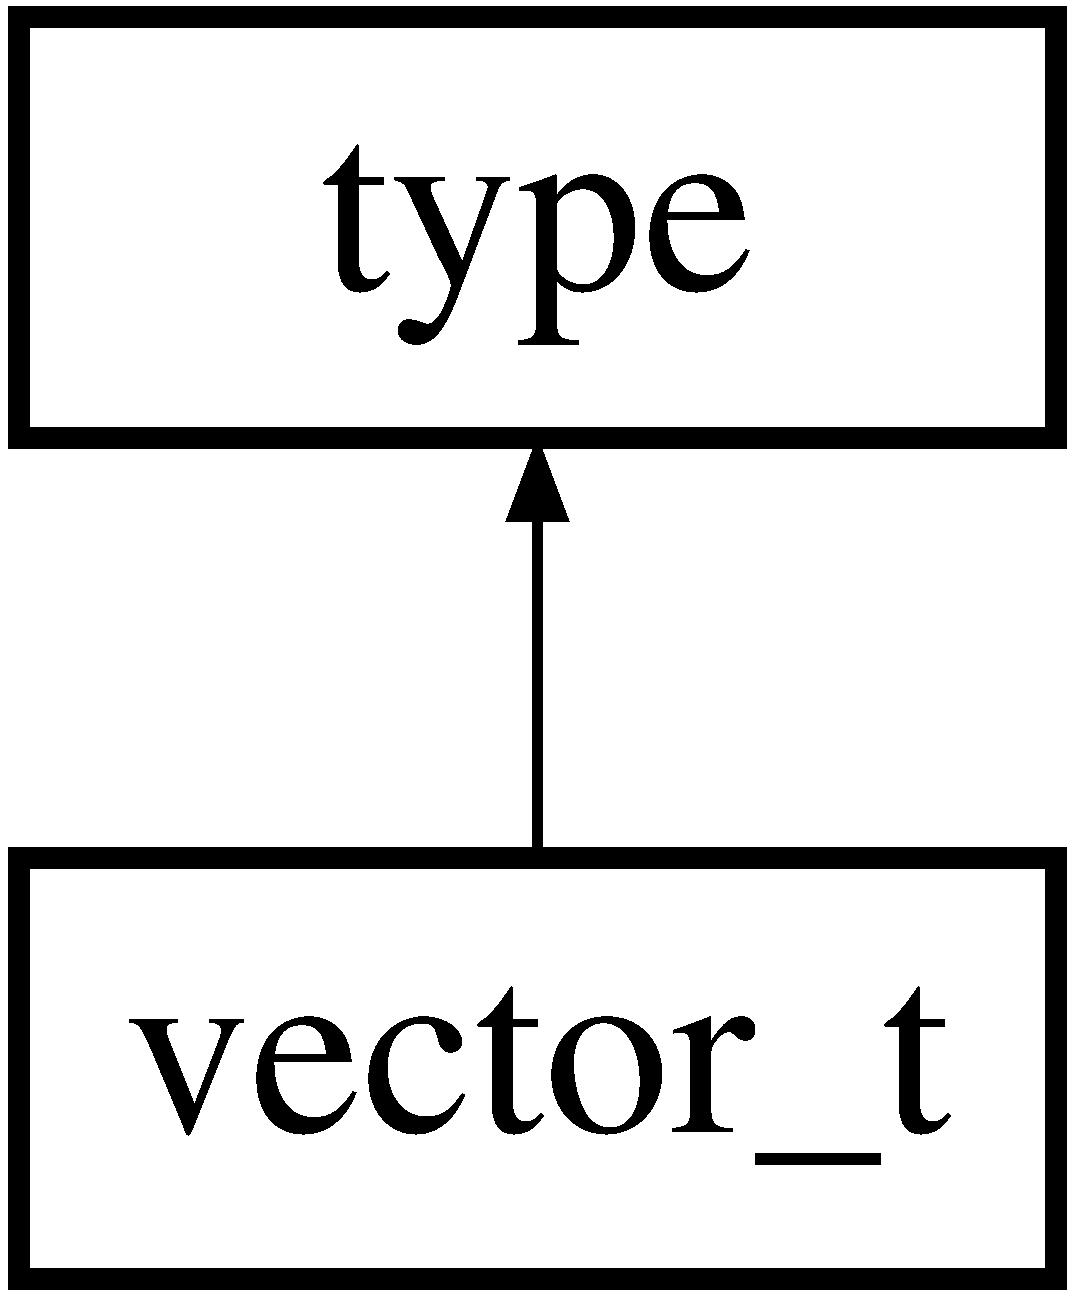
\includegraphics[height=2.000000cm]{classvector__t}
\end{center}
\end{figure}
\subsection*{Public Types}
\begin{DoxyCompactItemize}
\item 
typedef \+::\hyperlink{namespacexml__schema_ad7e04ab17bba0b3fdde43fb79ef6ed87}{xml\+\_\+schema\+::float\+\_\+} \hyperlink{classvector__t_a3e09c311dbbdc507b68a2f3fa0c3d25b}{x\+\_\+type}
\item 
typedef \+::xsd\+::cxx\+::tree\+::traits$<$ \hyperlink{classvector__t_a3e09c311dbbdc507b68a2f3fa0c3d25b}{x\+\_\+type}, char $>$ \hyperlink{classvector__t_ae5816c2392b8a96d1f1b44725329edef}{x\+\_\+traits}
\item 
typedef \+::\hyperlink{namespacexml__schema_ad7e04ab17bba0b3fdde43fb79ef6ed87}{xml\+\_\+schema\+::float\+\_\+} \hyperlink{classvector__t_ab24cc76c51c8a32d39f97d1b4f8ddc5c}{y\+\_\+type}
\item 
typedef \+::xsd\+::cxx\+::tree\+::traits$<$ \hyperlink{classvector__t_ab24cc76c51c8a32d39f97d1b4f8ddc5c}{y\+\_\+type}, char $>$ \hyperlink{classvector__t_a62b2a4701ddd5ad8548e19b50dbce8bb}{y\+\_\+traits}
\item 
typedef \+::\hyperlink{namespacexml__schema_ad7e04ab17bba0b3fdde43fb79ef6ed87}{xml\+\_\+schema\+::float\+\_\+} \hyperlink{classvector__t_a99f7b43996ec66480576ae8bd8d03cb6}{z\+\_\+type}
\item 
typedef \+::xsd\+::cxx\+::tree\+::traits$<$ \hyperlink{classvector__t_a99f7b43996ec66480576ae8bd8d03cb6}{z\+\_\+type}, char $>$ \hyperlink{classvector__t_a9ce39db28963631b425266d992cef7e3}{z\+\_\+traits}
\end{DoxyCompactItemize}
\subsection*{Public Member Functions}
\begin{DoxyCompactItemize}
\item 
const \hyperlink{classvector__t_a3e09c311dbbdc507b68a2f3fa0c3d25b}{x\+\_\+type} \& \hyperlink{classvector__t_a2b3fbe3ac4e41a57bcd63384ac1cc45e}{x} () const 
\item 
\hyperlink{classvector__t_a3e09c311dbbdc507b68a2f3fa0c3d25b}{x\+\_\+type} \& \hyperlink{classvector__t_a5ad3ab9e562b1344f5f8b5a068b4f30a}{x} ()
\item 
void \hyperlink{classvector__t_aa5d1f1a560eee9010dbe365d0a9ec764}{x} (const \hyperlink{classvector__t_a3e09c311dbbdc507b68a2f3fa0c3d25b}{x\+\_\+type} \&x)
\item 
const \hyperlink{classvector__t_ab24cc76c51c8a32d39f97d1b4f8ddc5c}{y\+\_\+type} \& \hyperlink{classvector__t_a678cf006ff3923c69574fc026e497fa4}{y} () const 
\item 
\hyperlink{classvector__t_ab24cc76c51c8a32d39f97d1b4f8ddc5c}{y\+\_\+type} \& \hyperlink{classvector__t_a89e4eb27037aac5823bfcd3b83012325}{y} ()
\item 
void \hyperlink{classvector__t_a0d70c752be7e0a8a53c988f0a851606a}{y} (const \hyperlink{classvector__t_ab24cc76c51c8a32d39f97d1b4f8ddc5c}{y\+\_\+type} \&\hyperlink{classvector__t_a2b3fbe3ac4e41a57bcd63384ac1cc45e}{x})
\item 
const \hyperlink{classvector__t_a99f7b43996ec66480576ae8bd8d03cb6}{z\+\_\+type} \& \hyperlink{classvector__t_ade029a7db60c9da0414b0acc46bbc2f3}{z} () const 
\item 
\hyperlink{classvector__t_a99f7b43996ec66480576ae8bd8d03cb6}{z\+\_\+type} \& \hyperlink{classvector__t_a2e2e70752783b23ed256e8144705f72b}{z} ()
\item 
void \hyperlink{classvector__t_ada2f0998eccbb4e8731249bcbdaad273}{z} (const \hyperlink{classvector__t_a99f7b43996ec66480576ae8bd8d03cb6}{z\+\_\+type} \&\hyperlink{classvector__t_a2b3fbe3ac4e41a57bcd63384ac1cc45e}{x})
\item 
\hyperlink{classvector__t_abff727e8dc18463cffcca860c76e63c0}{vector\+\_\+t} (const \hyperlink{classvector__t_a3e09c311dbbdc507b68a2f3fa0c3d25b}{x\+\_\+type} \&, const \hyperlink{classvector__t_ab24cc76c51c8a32d39f97d1b4f8ddc5c}{y\+\_\+type} \&, const \hyperlink{classvector__t_a99f7b43996ec66480576ae8bd8d03cb6}{z\+\_\+type} \&)
\item 
\hyperlink{classvector__t_a3ecb720954ae8b8b5e4a6c39bcc57618}{vector\+\_\+t} (const \+::xercesc\+::\+D\+O\+M\+Element \&e,\+::\hyperlink{namespacexml__schema_a0612287d030cb2732d31a45b258fdc87}{xml\+\_\+schema\+::flags} f=0,\+::\hyperlink{namespacexml__schema_ada9aa30dc722e93ee2ed7243085402a5}{xml\+\_\+schema\+::container} $\ast$c=0)
\item 
\hyperlink{classvector__t_a5bb219af224d0e0c8519a7d6028f8ab3}{vector\+\_\+t} (const \hyperlink{classvector__t}{vector\+\_\+t} \&\hyperlink{classvector__t_a2b3fbe3ac4e41a57bcd63384ac1cc45e}{x},\+::\hyperlink{namespacexml__schema_a0612287d030cb2732d31a45b258fdc87}{xml\+\_\+schema\+::flags} f=0,\+::\hyperlink{namespacexml__schema_ada9aa30dc722e93ee2ed7243085402a5}{xml\+\_\+schema\+::container} $\ast$c=0)
\item 
virtual \hyperlink{classvector__t}{vector\+\_\+t} $\ast$ \hyperlink{classvector__t_af377028533949e4849e342ede7cdab89}{\+\_\+clone} (\+::\hyperlink{namespacexml__schema_a0612287d030cb2732d31a45b258fdc87}{xml\+\_\+schema\+::flags} f=0,\+::\hyperlink{namespacexml__schema_ada9aa30dc722e93ee2ed7243085402a5}{xml\+\_\+schema\+::container} $\ast$c=0) const 
\item 
\hyperlink{classvector__t}{vector\+\_\+t} \& \hyperlink{classvector__t_ac7b3b90f82005375a5b348c086f42c72}{operator=} (const \hyperlink{classvector__t}{vector\+\_\+t} \&\hyperlink{classvector__t_a2b3fbe3ac4e41a57bcd63384ac1cc45e}{x})
\item 
virtual \hyperlink{classvector__t_a34b97db855d4c7d3eae880334900c49d}{$\sim$vector\+\_\+t} ()
\end{DoxyCompactItemize}
\subsection*{Protected Member Functions}
\begin{DoxyCompactItemize}
\item 
void \hyperlink{classvector__t_a003f2489abfa6c41c8a00423a1e021b7}{parse} (\+::xsd\+::cxx\+::xml\+::dom\+::parser$<$ char $>$ \&,\+::\hyperlink{namespacexml__schema_a0612287d030cb2732d31a45b258fdc87}{xml\+\_\+schema\+::flags})
\end{DoxyCompactItemize}
\subsection*{Protected Attributes}
\begin{DoxyCompactItemize}
\item 
\+::xsd\+::cxx\+::tree\+::one$<$ \hyperlink{classvector__t_a3e09c311dbbdc507b68a2f3fa0c3d25b}{x\+\_\+type} $>$ \hyperlink{classvector__t_a1769255617bd2fa4eacf02eacc65bc0e}{x\+\_\+}
\item 
\+::xsd\+::cxx\+::tree\+::one$<$ \hyperlink{classvector__t_ab24cc76c51c8a32d39f97d1b4f8ddc5c}{y\+\_\+type} $>$ \hyperlink{classvector__t_a973f8fd664c354e97518ca735124b7a2}{y\+\_\+}
\item 
\+::xsd\+::cxx\+::tree\+::one$<$ \hyperlink{classvector__t_a99f7b43996ec66480576ae8bd8d03cb6}{z\+\_\+type} $>$ \hyperlink{classvector__t_ac5887bca2fcd6cccde2e3cfdd3477108}{z\+\_\+}
\end{DoxyCompactItemize}


\subsection{Member Typedef Documentation}
\index{vector\+\_\+t@{vector\+\_\+t}!x\+\_\+traits@{x\+\_\+traits}}
\index{x\+\_\+traits@{x\+\_\+traits}!vector\+\_\+t@{vector\+\_\+t}}
\subsubsection[{\texorpdfstring{x\+\_\+traits}{x_traits}}]{\setlength{\rightskip}{0pt plus 5cm}typedef \+::xsd\+::cxx\+::tree\+::traits$<$ {\bf x\+\_\+type}, char $>$ {\bf vector\+\_\+t\+::x\+\_\+traits}}\hypertarget{classvector__t_ae5816c2392b8a96d1f1b44725329edef}{}\label{classvector__t_ae5816c2392b8a96d1f1b44725329edef}
\index{vector\+\_\+t@{vector\+\_\+t}!x\+\_\+type@{x\+\_\+type}}
\index{x\+\_\+type@{x\+\_\+type}!vector\+\_\+t@{vector\+\_\+t}}
\subsubsection[{\texorpdfstring{x\+\_\+type}{x_type}}]{\setlength{\rightskip}{0pt plus 5cm}typedef \+::{\bf xml\+\_\+schema\+::float\+\_\+} {\bf vector\+\_\+t\+::x\+\_\+type}}\hypertarget{classvector__t_a3e09c311dbbdc507b68a2f3fa0c3d25b}{}\label{classvector__t_a3e09c311dbbdc507b68a2f3fa0c3d25b}
\index{vector\+\_\+t@{vector\+\_\+t}!y\+\_\+traits@{y\+\_\+traits}}
\index{y\+\_\+traits@{y\+\_\+traits}!vector\+\_\+t@{vector\+\_\+t}}
\subsubsection[{\texorpdfstring{y\+\_\+traits}{y_traits}}]{\setlength{\rightskip}{0pt plus 5cm}typedef \+::xsd\+::cxx\+::tree\+::traits$<$ {\bf y\+\_\+type}, char $>$ {\bf vector\+\_\+t\+::y\+\_\+traits}}\hypertarget{classvector__t_a62b2a4701ddd5ad8548e19b50dbce8bb}{}\label{classvector__t_a62b2a4701ddd5ad8548e19b50dbce8bb}
\index{vector\+\_\+t@{vector\+\_\+t}!y\+\_\+type@{y\+\_\+type}}
\index{y\+\_\+type@{y\+\_\+type}!vector\+\_\+t@{vector\+\_\+t}}
\subsubsection[{\texorpdfstring{y\+\_\+type}{y_type}}]{\setlength{\rightskip}{0pt plus 5cm}typedef \+::{\bf xml\+\_\+schema\+::float\+\_\+} {\bf vector\+\_\+t\+::y\+\_\+type}}\hypertarget{classvector__t_ab24cc76c51c8a32d39f97d1b4f8ddc5c}{}\label{classvector__t_ab24cc76c51c8a32d39f97d1b4f8ddc5c}
\index{vector\+\_\+t@{vector\+\_\+t}!z\+\_\+traits@{z\+\_\+traits}}
\index{z\+\_\+traits@{z\+\_\+traits}!vector\+\_\+t@{vector\+\_\+t}}
\subsubsection[{\texorpdfstring{z\+\_\+traits}{z_traits}}]{\setlength{\rightskip}{0pt plus 5cm}typedef \+::xsd\+::cxx\+::tree\+::traits$<$ {\bf z\+\_\+type}, char $>$ {\bf vector\+\_\+t\+::z\+\_\+traits}}\hypertarget{classvector__t_a9ce39db28963631b425266d992cef7e3}{}\label{classvector__t_a9ce39db28963631b425266d992cef7e3}
\index{vector\+\_\+t@{vector\+\_\+t}!z\+\_\+type@{z\+\_\+type}}
\index{z\+\_\+type@{z\+\_\+type}!vector\+\_\+t@{vector\+\_\+t}}
\subsubsection[{\texorpdfstring{z\+\_\+type}{z_type}}]{\setlength{\rightskip}{0pt plus 5cm}typedef \+::{\bf xml\+\_\+schema\+::float\+\_\+} {\bf vector\+\_\+t\+::z\+\_\+type}}\hypertarget{classvector__t_a99f7b43996ec66480576ae8bd8d03cb6}{}\label{classvector__t_a99f7b43996ec66480576ae8bd8d03cb6}


\subsection{Constructor \& Destructor Documentation}
\index{vector\+\_\+t@{vector\+\_\+t}!vector\+\_\+t@{vector\+\_\+t}}
\index{vector\+\_\+t@{vector\+\_\+t}!vector\+\_\+t@{vector\+\_\+t}}
\subsubsection[{\texorpdfstring{vector\+\_\+t(const x\+\_\+type \&, const y\+\_\+type \&, const z\+\_\+type \&)}{vector_t(const x_type &, const y_type &, const z_type &)}}]{\setlength{\rightskip}{0pt plus 5cm}vector\+\_\+t\+::vector\+\_\+t (
\begin{DoxyParamCaption}
\item[{const {\bf x\+\_\+type} \&}]{x, }
\item[{const {\bf y\+\_\+type} \&}]{y, }
\item[{const {\bf z\+\_\+type} \&}]{z}
\end{DoxyParamCaption}
)}\hypertarget{classvector__t_abff727e8dc18463cffcca860c76e63c0}{}\label{classvector__t_abff727e8dc18463cffcca860c76e63c0}
\index{vector\+\_\+t@{vector\+\_\+t}!vector\+\_\+t@{vector\+\_\+t}}
\index{vector\+\_\+t@{vector\+\_\+t}!vector\+\_\+t@{vector\+\_\+t}}
\subsubsection[{\texorpdfstring{vector\+\_\+t(const \+::xercesc\+::\+D\+O\+M\+Element \&e,\+::xml\+\_\+schema\+::flags f=0,\+::xml\+\_\+schema\+::container $\ast$c=0)}{vector_t(const ::xercesc::DOMElement &e,::xml_schema::flags f=0,::xml_schema::container *c=0)}}]{\setlength{\rightskip}{0pt plus 5cm}vector\+\_\+t\+::vector\+\_\+t (
\begin{DoxyParamCaption}
\item[{const \+::xercesc\+::\+D\+O\+M\+Element \&}]{e, }
\item[{\+::{\bf xml\+\_\+schema\+::flags}}]{f = {\ttfamily 0}, }
\item[{\+::{\bf xml\+\_\+schema\+::container} $\ast$}]{c = {\ttfamily 0}}
\end{DoxyParamCaption}
)}\hypertarget{classvector__t_a3ecb720954ae8b8b5e4a6c39bcc57618}{}\label{classvector__t_a3ecb720954ae8b8b5e4a6c39bcc57618}
\index{vector\+\_\+t@{vector\+\_\+t}!vector\+\_\+t@{vector\+\_\+t}}
\index{vector\+\_\+t@{vector\+\_\+t}!vector\+\_\+t@{vector\+\_\+t}}
\subsubsection[{\texorpdfstring{vector\+\_\+t(const vector\+\_\+t \&x,\+::xml\+\_\+schema\+::flags f=0,\+::xml\+\_\+schema\+::container $\ast$c=0)}{vector_t(const vector_t &x,::xml_schema::flags f=0,::xml_schema::container *c=0)}}]{\setlength{\rightskip}{0pt plus 5cm}vector\+\_\+t\+::vector\+\_\+t (
\begin{DoxyParamCaption}
\item[{const {\bf vector\+\_\+t} \&}]{x, }
\item[{\+::{\bf xml\+\_\+schema\+::flags}}]{f = {\ttfamily 0}, }
\item[{\+::{\bf xml\+\_\+schema\+::container} $\ast$}]{c = {\ttfamily 0}}
\end{DoxyParamCaption}
)}\hypertarget{classvector__t_a5bb219af224d0e0c8519a7d6028f8ab3}{}\label{classvector__t_a5bb219af224d0e0c8519a7d6028f8ab3}
\index{vector\+\_\+t@{vector\+\_\+t}!````~vector\+\_\+t@{$\sim$vector\+\_\+t}}
\index{````~vector\+\_\+t@{$\sim$vector\+\_\+t}!vector\+\_\+t@{vector\+\_\+t}}
\subsubsection[{\texorpdfstring{$\sim$vector\+\_\+t()}{~vector_t()}}]{\setlength{\rightskip}{0pt plus 5cm}vector\+\_\+t\+::$\sim$vector\+\_\+t (
\begin{DoxyParamCaption}
{}
\end{DoxyParamCaption}
)\hspace{0.3cm}{\ttfamily [virtual]}}\hypertarget{classvector__t_a34b97db855d4c7d3eae880334900c49d}{}\label{classvector__t_a34b97db855d4c7d3eae880334900c49d}


\subsection{Member Function Documentation}
\index{vector\+\_\+t@{vector\+\_\+t}!\+\_\+clone@{\+\_\+clone}}
\index{\+\_\+clone@{\+\_\+clone}!vector\+\_\+t@{vector\+\_\+t}}
\subsubsection[{\texorpdfstring{\+\_\+clone(\+::xml\+\_\+schema\+::flags f=0,\+::xml\+\_\+schema\+::container $\ast$c=0) const }{_clone(::xml_schema::flags f=0,::xml_schema::container *c=0) const }}]{\setlength{\rightskip}{0pt plus 5cm}{\bf vector\+\_\+t} $\ast$ vector\+\_\+t\+::\+\_\+clone (
\begin{DoxyParamCaption}
\item[{\+::{\bf xml\+\_\+schema\+::flags}}]{f = {\ttfamily 0}, }
\item[{\+::{\bf xml\+\_\+schema\+::container} $\ast$}]{c = {\ttfamily 0}}
\end{DoxyParamCaption}
) const\hspace{0.3cm}{\ttfamily [virtual]}}\hypertarget{classvector__t_af377028533949e4849e342ede7cdab89}{}\label{classvector__t_af377028533949e4849e342ede7cdab89}
\index{vector\+\_\+t@{vector\+\_\+t}!operator=@{operator=}}
\index{operator=@{operator=}!vector\+\_\+t@{vector\+\_\+t}}
\subsubsection[{\texorpdfstring{operator=(const vector\+\_\+t \&x)}{operator=(const vector_t &x)}}]{\setlength{\rightskip}{0pt plus 5cm}{\bf vector\+\_\+t} \& vector\+\_\+t\+::operator= (
\begin{DoxyParamCaption}
\item[{const {\bf vector\+\_\+t} \&}]{x}
\end{DoxyParamCaption}
)}\hypertarget{classvector__t_ac7b3b90f82005375a5b348c086f42c72}{}\label{classvector__t_ac7b3b90f82005375a5b348c086f42c72}
\index{vector\+\_\+t@{vector\+\_\+t}!parse@{parse}}
\index{parse@{parse}!vector\+\_\+t@{vector\+\_\+t}}
\subsubsection[{\texorpdfstring{parse(\+::xsd\+::cxx\+::xml\+::dom\+::parser$<$ char $>$ \&,\+::xml\+\_\+schema\+::flags)}{parse(::xsd::cxx::xml::dom::parser< char > &,::xml_schema::flags)}}]{\setlength{\rightskip}{0pt plus 5cm}void vector\+\_\+t\+::parse (
\begin{DoxyParamCaption}
\item[{\+::xsd\+::cxx\+::xml\+::dom\+::parser$<$ char $>$ \&}]{p, }
\item[{\+::{\bf xml\+\_\+schema\+::flags}}]{f}
\end{DoxyParamCaption}
)\hspace{0.3cm}{\ttfamily [protected]}}\hypertarget{classvector__t_a003f2489abfa6c41c8a00423a1e021b7}{}\label{classvector__t_a003f2489abfa6c41c8a00423a1e021b7}
\index{vector\+\_\+t@{vector\+\_\+t}!x@{x}}
\index{x@{x}!vector\+\_\+t@{vector\+\_\+t}}
\subsubsection[{\texorpdfstring{x() const }{x() const }}]{\setlength{\rightskip}{0pt plus 5cm}const {\bf vector\+\_\+t\+::x\+\_\+type} \& vector\+\_\+t\+::x (
\begin{DoxyParamCaption}
{}
\end{DoxyParamCaption}
) const}\hypertarget{classvector__t_a2b3fbe3ac4e41a57bcd63384ac1cc45e}{}\label{classvector__t_a2b3fbe3ac4e41a57bcd63384ac1cc45e}
\index{vector\+\_\+t@{vector\+\_\+t}!x@{x}}
\index{x@{x}!vector\+\_\+t@{vector\+\_\+t}}
\subsubsection[{\texorpdfstring{x()}{x()}}]{\setlength{\rightskip}{0pt plus 5cm}{\bf vector\+\_\+t\+::x\+\_\+type} \& vector\+\_\+t\+::x (
\begin{DoxyParamCaption}
{}
\end{DoxyParamCaption}
)}\hypertarget{classvector__t_a5ad3ab9e562b1344f5f8b5a068b4f30a}{}\label{classvector__t_a5ad3ab9e562b1344f5f8b5a068b4f30a}
\index{vector\+\_\+t@{vector\+\_\+t}!x@{x}}
\index{x@{x}!vector\+\_\+t@{vector\+\_\+t}}
\subsubsection[{\texorpdfstring{x(const x\+\_\+type \&x)}{x(const x_type &x)}}]{\setlength{\rightskip}{0pt plus 5cm}void vector\+\_\+t\+::x (
\begin{DoxyParamCaption}
\item[{const {\bf x\+\_\+type} \&}]{x}
\end{DoxyParamCaption}
)}\hypertarget{classvector__t_aa5d1f1a560eee9010dbe365d0a9ec764}{}\label{classvector__t_aa5d1f1a560eee9010dbe365d0a9ec764}
\index{vector\+\_\+t@{vector\+\_\+t}!y@{y}}
\index{y@{y}!vector\+\_\+t@{vector\+\_\+t}}
\subsubsection[{\texorpdfstring{y() const }{y() const }}]{\setlength{\rightskip}{0pt plus 5cm}const {\bf vector\+\_\+t\+::y\+\_\+type} \& vector\+\_\+t\+::y (
\begin{DoxyParamCaption}
{}
\end{DoxyParamCaption}
) const}\hypertarget{classvector__t_a678cf006ff3923c69574fc026e497fa4}{}\label{classvector__t_a678cf006ff3923c69574fc026e497fa4}
\index{vector\+\_\+t@{vector\+\_\+t}!y@{y}}
\index{y@{y}!vector\+\_\+t@{vector\+\_\+t}}
\subsubsection[{\texorpdfstring{y()}{y()}}]{\setlength{\rightskip}{0pt plus 5cm}{\bf vector\+\_\+t\+::y\+\_\+type} \& vector\+\_\+t\+::y (
\begin{DoxyParamCaption}
{}
\end{DoxyParamCaption}
)}\hypertarget{classvector__t_a89e4eb27037aac5823bfcd3b83012325}{}\label{classvector__t_a89e4eb27037aac5823bfcd3b83012325}
\index{vector\+\_\+t@{vector\+\_\+t}!y@{y}}
\index{y@{y}!vector\+\_\+t@{vector\+\_\+t}}
\subsubsection[{\texorpdfstring{y(const y\+\_\+type \&x)}{y(const y_type &x)}}]{\setlength{\rightskip}{0pt plus 5cm}void vector\+\_\+t\+::y (
\begin{DoxyParamCaption}
\item[{const {\bf y\+\_\+type} \&}]{x}
\end{DoxyParamCaption}
)}\hypertarget{classvector__t_a0d70c752be7e0a8a53c988f0a851606a}{}\label{classvector__t_a0d70c752be7e0a8a53c988f0a851606a}
\index{vector\+\_\+t@{vector\+\_\+t}!z@{z}}
\index{z@{z}!vector\+\_\+t@{vector\+\_\+t}}
\subsubsection[{\texorpdfstring{z() const }{z() const }}]{\setlength{\rightskip}{0pt plus 5cm}const {\bf vector\+\_\+t\+::z\+\_\+type} \& vector\+\_\+t\+::z (
\begin{DoxyParamCaption}
{}
\end{DoxyParamCaption}
) const}\hypertarget{classvector__t_ade029a7db60c9da0414b0acc46bbc2f3}{}\label{classvector__t_ade029a7db60c9da0414b0acc46bbc2f3}
\index{vector\+\_\+t@{vector\+\_\+t}!z@{z}}
\index{z@{z}!vector\+\_\+t@{vector\+\_\+t}}
\subsubsection[{\texorpdfstring{z()}{z()}}]{\setlength{\rightskip}{0pt plus 5cm}{\bf vector\+\_\+t\+::z\+\_\+type} \& vector\+\_\+t\+::z (
\begin{DoxyParamCaption}
{}
\end{DoxyParamCaption}
)}\hypertarget{classvector__t_a2e2e70752783b23ed256e8144705f72b}{}\label{classvector__t_a2e2e70752783b23ed256e8144705f72b}
\index{vector\+\_\+t@{vector\+\_\+t}!z@{z}}
\index{z@{z}!vector\+\_\+t@{vector\+\_\+t}}
\subsubsection[{\texorpdfstring{z(const z\+\_\+type \&x)}{z(const z_type &x)}}]{\setlength{\rightskip}{0pt plus 5cm}void vector\+\_\+t\+::z (
\begin{DoxyParamCaption}
\item[{const {\bf z\+\_\+type} \&}]{x}
\end{DoxyParamCaption}
)}\hypertarget{classvector__t_ada2f0998eccbb4e8731249bcbdaad273}{}\label{classvector__t_ada2f0998eccbb4e8731249bcbdaad273}


\subsection{Member Data Documentation}
\index{vector\+\_\+t@{vector\+\_\+t}!x\+\_\+@{x\+\_\+}}
\index{x\+\_\+@{x\+\_\+}!vector\+\_\+t@{vector\+\_\+t}}
\subsubsection[{\texorpdfstring{x\+\_\+}{x_}}]{\setlength{\rightskip}{0pt plus 5cm}\+::xsd\+::cxx\+::tree\+::one$<$ {\bf x\+\_\+type} $>$ vector\+\_\+t\+::x\+\_\+\hspace{0.3cm}{\ttfamily [protected]}}\hypertarget{classvector__t_a1769255617bd2fa4eacf02eacc65bc0e}{}\label{classvector__t_a1769255617bd2fa4eacf02eacc65bc0e}
\index{vector\+\_\+t@{vector\+\_\+t}!y\+\_\+@{y\+\_\+}}
\index{y\+\_\+@{y\+\_\+}!vector\+\_\+t@{vector\+\_\+t}}
\subsubsection[{\texorpdfstring{y\+\_\+}{y_}}]{\setlength{\rightskip}{0pt plus 5cm}\+::xsd\+::cxx\+::tree\+::one$<$ {\bf y\+\_\+type} $>$ vector\+\_\+t\+::y\+\_\+\hspace{0.3cm}{\ttfamily [protected]}}\hypertarget{classvector__t_a973f8fd664c354e97518ca735124b7a2}{}\label{classvector__t_a973f8fd664c354e97518ca735124b7a2}
\index{vector\+\_\+t@{vector\+\_\+t}!z\+\_\+@{z\+\_\+}}
\index{z\+\_\+@{z\+\_\+}!vector\+\_\+t@{vector\+\_\+t}}
\subsubsection[{\texorpdfstring{z\+\_\+}{z_}}]{\setlength{\rightskip}{0pt plus 5cm}\+::xsd\+::cxx\+::tree\+::one$<$ {\bf z\+\_\+type} $>$ vector\+\_\+t\+::z\+\_\+\hspace{0.3cm}{\ttfamily [protected]}}\hypertarget{classvector__t_ac5887bca2fcd6cccde2e3cfdd3477108}{}\label{classvector__t_ac5887bca2fcd6cccde2e3cfdd3477108}


The documentation for this class was generated from the following files\+:\begin{DoxyCompactItemize}
\item 
src/input/\hyperlink{particle__input_8h}{particle\+\_\+input.\+h}\item 
src/input/\hyperlink{particle__input_8cpp}{particle\+\_\+input.\+cpp}\end{DoxyCompactItemize}

\hypertarget{classVTKFile__t}{}\section{V\+T\+K\+File\+\_\+t Class Reference}
\label{classVTKFile__t}\index{V\+T\+K\+File\+\_\+t@{V\+T\+K\+File\+\_\+t}}


{\ttfamily \#include $<$vtk-\/unstructured.\+h$>$}

Inheritance diagram for V\+T\+K\+File\+\_\+t\+:\begin{figure}[H]
\begin{center}
\leavevmode
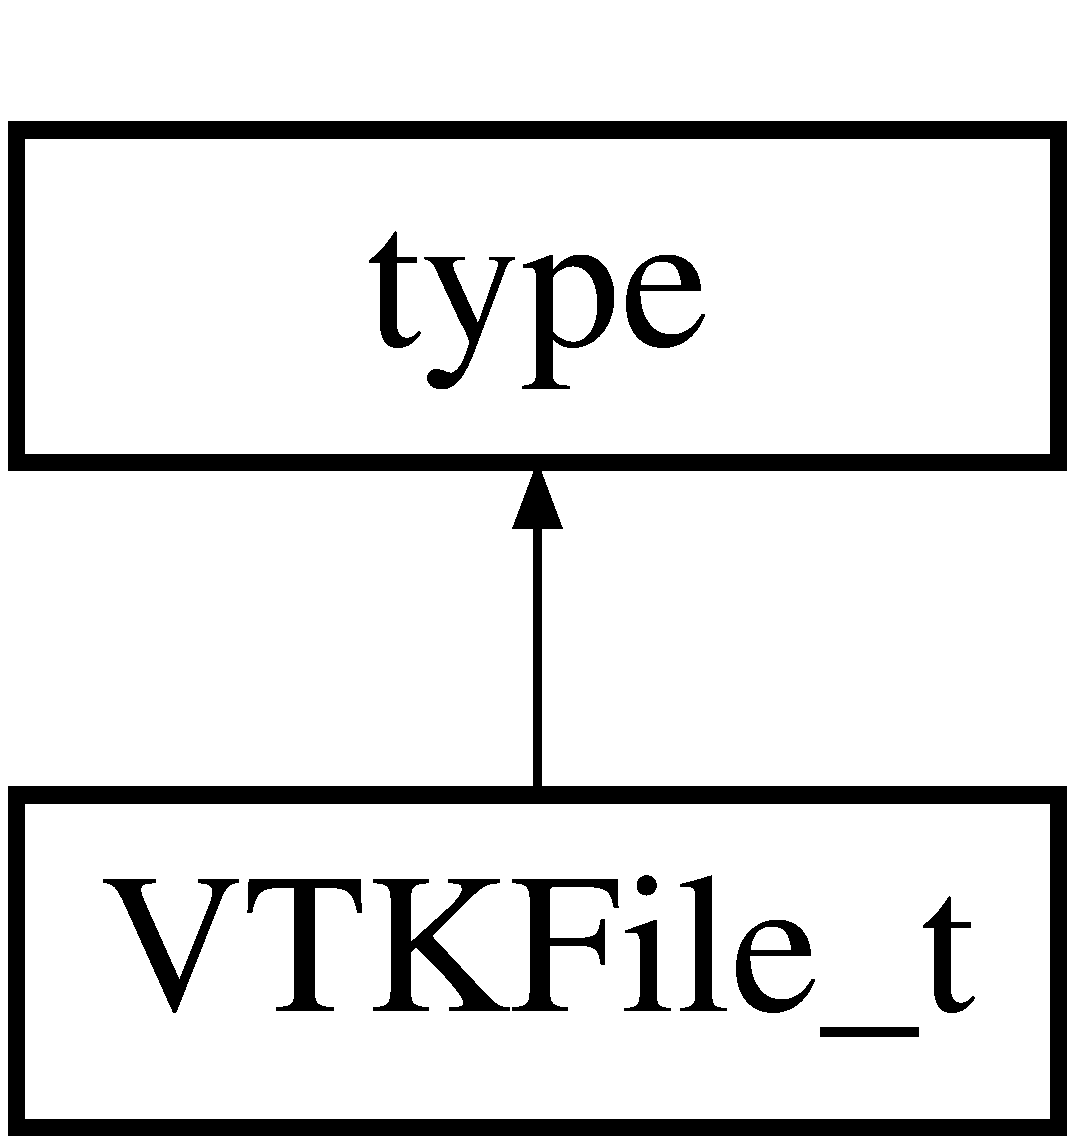
\includegraphics[height=2.000000cm]{classVTKFile__t}
\end{center}
\end{figure}
\subsection*{Public Types}
\begin{DoxyCompactItemize}
\item 
typedef \+::\hyperlink{classUnstructuredGrid__t}{Unstructured\+Grid\+\_\+t} \hyperlink{classVTKFile__t_a34ea02f6804e701657f11a8dc3851951}{Unstructured\+Grid\+\_\+type}
\item 
typedef \+::xsd\+::cxx\+::tree\+::optional$<$ \hyperlink{classVTKFile__t_a34ea02f6804e701657f11a8dc3851951}{Unstructured\+Grid\+\_\+type} $>$ \hyperlink{classVTKFile__t_ada5bb5a706e03ef1ab2ed1513ea83833}{Unstructured\+Grid\+\_\+optional}
\item 
typedef \+::xsd\+::cxx\+::tree\+::traits$<$ \hyperlink{classVTKFile__t_a34ea02f6804e701657f11a8dc3851951}{Unstructured\+Grid\+\_\+type}, char $>$ \hyperlink{classVTKFile__t_a02772a5f713678f02e94188d6a552528}{Unstructured\+Grid\+\_\+traits}
\item 
typedef \+::\hyperlink{classPolyData__t}{Poly\+Data\+\_\+t} \hyperlink{classVTKFile__t_a4588b4f0e28ba09aa219bda7e1fc6c97}{Poly\+Data\+\_\+type}
\item 
typedef \+::xsd\+::cxx\+::tree\+::optional$<$ \hyperlink{classVTKFile__t_a4588b4f0e28ba09aa219bda7e1fc6c97}{Poly\+Data\+\_\+type} $>$ \hyperlink{classVTKFile__t_aacb796775ae228cd61726a23b809f3e4}{Poly\+Data\+\_\+optional}
\item 
typedef \+::xsd\+::cxx\+::tree\+::traits$<$ \hyperlink{classVTKFile__t_a4588b4f0e28ba09aa219bda7e1fc6c97}{Poly\+Data\+\_\+type}, char $>$ \hyperlink{classVTKFile__t_aa5ad98f5709c1e9beec3804a7f42b5f6}{Poly\+Data\+\_\+traits}
\item 
typedef \+::\hyperlink{namespacexml__schema_ac0cec83a330f0024e4e318b3deac5104}{xml\+\_\+schema\+::string} \hyperlink{classVTKFile__t_ac1f3484e4fde414849ede43a00955f76}{type\+\_\+type}
\item 
typedef \+::xsd\+::cxx\+::tree\+::traits$<$ \hyperlink{classVTKFile__t_ac1f3484e4fde414849ede43a00955f76}{type\+\_\+type}, char $>$ \hyperlink{classVTKFile__t_aee4ac167e843e9def1be4f43ad930391}{type\+\_\+traits}
\item 
typedef \+::\hyperlink{namespacexml__schema_ac0cec83a330f0024e4e318b3deac5104}{xml\+\_\+schema\+::string} \hyperlink{classVTKFile__t_a7db6f6d11f363380d6361446f5dede7b}{version\+\_\+type}
\item 
typedef \+::xsd\+::cxx\+::tree\+::traits$<$ \hyperlink{classVTKFile__t_a7db6f6d11f363380d6361446f5dede7b}{version\+\_\+type}, char $>$ \hyperlink{classVTKFile__t_a5a343e08417564e5db3f48859b1a0c5f}{version\+\_\+traits}
\item 
typedef \+::\hyperlink{namespacexml__schema_ac0cec83a330f0024e4e318b3deac5104}{xml\+\_\+schema\+::string} \hyperlink{classVTKFile__t_ab08dd45c560dd0635d0e5c0a5e42d2e8}{byte\+\_\+order\+\_\+type}
\item 
typedef \+::xsd\+::cxx\+::tree\+::traits$<$ \hyperlink{classVTKFile__t_ab08dd45c560dd0635d0e5c0a5e42d2e8}{byte\+\_\+order\+\_\+type}, char $>$ \hyperlink{classVTKFile__t_ae0b8c254bc373d9218ea9eab406b7b98}{byte\+\_\+order\+\_\+traits}
\end{DoxyCompactItemize}
\subsection*{Public Member Functions}
\begin{DoxyCompactItemize}
\item 
const \hyperlink{classVTKFile__t_ada5bb5a706e03ef1ab2ed1513ea83833}{Unstructured\+Grid\+\_\+optional} \& \hyperlink{classVTKFile__t_a118852d8ec1f8039d1fd5c914282351a}{Unstructured\+Grid} () const 
\item 
\hyperlink{classVTKFile__t_ada5bb5a706e03ef1ab2ed1513ea83833}{Unstructured\+Grid\+\_\+optional} \& \hyperlink{classVTKFile__t_aa4746d4a723076d4643b8ef16a9c3890}{Unstructured\+Grid} ()
\item 
void \hyperlink{classVTKFile__t_a2c2b1b2ff487c7e61bcd2875db8747be}{Unstructured\+Grid} (const \hyperlink{classVTKFile__t_a34ea02f6804e701657f11a8dc3851951}{Unstructured\+Grid\+\_\+type} \&x)
\item 
void \hyperlink{classVTKFile__t_ae33d9781bddb747f9255570b1af2dfeb}{Unstructured\+Grid} (const \hyperlink{classVTKFile__t_ada5bb5a706e03ef1ab2ed1513ea83833}{Unstructured\+Grid\+\_\+optional} \&x)
\item 
void \hyperlink{classVTKFile__t_aa0971069bdc8c87a2b5b90f4e50dce3c}{Unstructured\+Grid} (\+::std\+::unique\+\_\+ptr$<$ \hyperlink{classVTKFile__t_a34ea02f6804e701657f11a8dc3851951}{Unstructured\+Grid\+\_\+type} $>$ p)
\item 
const \hyperlink{classVTKFile__t_aacb796775ae228cd61726a23b809f3e4}{Poly\+Data\+\_\+optional} \& \hyperlink{classVTKFile__t_a7d728d7f31157fc80117c2f80978344c}{Poly\+Data} () const 
\item 
\hyperlink{classVTKFile__t_aacb796775ae228cd61726a23b809f3e4}{Poly\+Data\+\_\+optional} \& \hyperlink{classVTKFile__t_a0f87118c1898bc43619fa0bade52e921}{Poly\+Data} ()
\item 
void \hyperlink{classVTKFile__t_ab0a3f2aa2894d0384a89a6e5490c9372}{Poly\+Data} (const \hyperlink{classVTKFile__t_a4588b4f0e28ba09aa219bda7e1fc6c97}{Poly\+Data\+\_\+type} \&x)
\item 
void \hyperlink{classVTKFile__t_a1c2a800d41431c04965c863220a3b1b5}{Poly\+Data} (const \hyperlink{classVTKFile__t_aacb796775ae228cd61726a23b809f3e4}{Poly\+Data\+\_\+optional} \&x)
\item 
void \hyperlink{classVTKFile__t_a3d4840c857ac2cc511849d537b003020}{Poly\+Data} (\+::std\+::unique\+\_\+ptr$<$ \hyperlink{classVTKFile__t_a4588b4f0e28ba09aa219bda7e1fc6c97}{Poly\+Data\+\_\+type} $>$ p)
\item 
const \hyperlink{classVTKFile__t_ac1f3484e4fde414849ede43a00955f76}{type\+\_\+type} \& \hyperlink{classVTKFile__t_a5c23301c79cc6a376fe2abce533b2cf7}{type} () const 
\item 
\hyperlink{classVTKFile__t_ac1f3484e4fde414849ede43a00955f76}{type\+\_\+type} \& \hyperlink{classVTKFile__t_abcc8ab822fa4f9e5e5294f5d8cff05c2}{type} ()
\item 
void \hyperlink{classVTKFile__t_a6423eb2dc7fa367417df87de4921301e}{type} (const \hyperlink{classVTKFile__t_ac1f3484e4fde414849ede43a00955f76}{type\+\_\+type} \&x)
\item 
void \hyperlink{classVTKFile__t_ac2dec76d5784d0f937c95932d8792e12}{type} (\+::std\+::unique\+\_\+ptr$<$ \hyperlink{classVTKFile__t_ac1f3484e4fde414849ede43a00955f76}{type\+\_\+type} $>$ p)
\item 
const \hyperlink{classVTKFile__t_a7db6f6d11f363380d6361446f5dede7b}{version\+\_\+type} \& \hyperlink{classVTKFile__t_af0f1ed9d44019ad1fab6495b6ae71a47}{version} () const 
\item 
const \hyperlink{classVTKFile__t_ab08dd45c560dd0635d0e5c0a5e42d2e8}{byte\+\_\+order\+\_\+type} \& \hyperlink{classVTKFile__t_ad87b4f45ca18139b1ffae8ce08dc2e27}{byte\+\_\+order} () const 
\item 
\hyperlink{classVTKFile__t_a76547340cb91ad0019d45889ca69fda0}{V\+T\+K\+File\+\_\+t} (const \hyperlink{classVTKFile__t_ac1f3484e4fde414849ede43a00955f76}{type\+\_\+type} \&)
\item 
\hyperlink{classVTKFile__t_a5d1c8c263c9865fe6f4b6ae1446efcaf}{V\+T\+K\+File\+\_\+t} (const \+::xercesc\+::\+D\+O\+M\+Element \&e,\+::\hyperlink{namespacexml__schema_a0612287d030cb2732d31a45b258fdc87}{xml\+\_\+schema\+::flags} f=0,\+::\hyperlink{namespacexml__schema_ada9aa30dc722e93ee2ed7243085402a5}{xml\+\_\+schema\+::container} $\ast$c=0)
\item 
\hyperlink{classVTKFile__t_af239970202f0aee8392cb0af61863f62}{V\+T\+K\+File\+\_\+t} (const \hyperlink{classVTKFile__t}{V\+T\+K\+File\+\_\+t} \&x,\+::\hyperlink{namespacexml__schema_a0612287d030cb2732d31a45b258fdc87}{xml\+\_\+schema\+::flags} f=0,\+::\hyperlink{namespacexml__schema_ada9aa30dc722e93ee2ed7243085402a5}{xml\+\_\+schema\+::container} $\ast$c=0)
\item 
virtual \hyperlink{classVTKFile__t}{V\+T\+K\+File\+\_\+t} $\ast$ \hyperlink{classVTKFile__t_ad39ce94f7390685f9717fd521bac36e3}{\+\_\+clone} (\+::\hyperlink{namespacexml__schema_a0612287d030cb2732d31a45b258fdc87}{xml\+\_\+schema\+::flags} f=0,\+::\hyperlink{namespacexml__schema_ada9aa30dc722e93ee2ed7243085402a5}{xml\+\_\+schema\+::container} $\ast$c=0) const 
\item 
\hyperlink{classVTKFile__t}{V\+T\+K\+File\+\_\+t} \& \hyperlink{classVTKFile__t_a0f2e74c4753d5c47f9e358ed50b4d2a3}{operator=} (const \hyperlink{classVTKFile__t}{V\+T\+K\+File\+\_\+t} \&x)
\item 
virtual \hyperlink{classVTKFile__t_ac5cf95c81660088dbb3c9ab6cd78dede}{$\sim$\+V\+T\+K\+File\+\_\+t} ()
\end{DoxyCompactItemize}
\subsection*{Static Public Member Functions}
\begin{DoxyCompactItemize}
\item 
static const \hyperlink{classVTKFile__t_a7db6f6d11f363380d6361446f5dede7b}{version\+\_\+type} \& \hyperlink{classVTKFile__t_a0eb5afa9ec6125c0519a891578f31521}{version\+\_\+default\+\_\+value} ()
\item 
static const \hyperlink{classVTKFile__t_ab08dd45c560dd0635d0e5c0a5e42d2e8}{byte\+\_\+order\+\_\+type} \& \hyperlink{classVTKFile__t_a4538fe428d79eff40025d874e200bec1}{byte\+\_\+order\+\_\+default\+\_\+value} ()
\end{DoxyCompactItemize}
\subsection*{Protected Member Functions}
\begin{DoxyCompactItemize}
\item 
void \hyperlink{classVTKFile__t_abce5eb0ea7f326f97fdbd8eeafc69dac}{parse} (\+::xsd\+::cxx\+::xml\+::dom\+::parser$<$ char $>$ \&,\+::\hyperlink{namespacexml__schema_a0612287d030cb2732d31a45b258fdc87}{xml\+\_\+schema\+::flags})
\end{DoxyCompactItemize}
\subsection*{Protected Attributes}
\begin{DoxyCompactItemize}
\item 
\hyperlink{classVTKFile__t_ada5bb5a706e03ef1ab2ed1513ea83833}{Unstructured\+Grid\+\_\+optional} \hyperlink{classVTKFile__t_a8ff0a1326731c3a73403f6a6fb46e0ac}{Unstructured\+Grid\+\_\+}
\item 
\hyperlink{classVTKFile__t_aacb796775ae228cd61726a23b809f3e4}{Poly\+Data\+\_\+optional} \hyperlink{classVTKFile__t_ae7de0b4fb3566ea6b7e4270c4f6560ef}{Poly\+Data\+\_\+}
\item 
\+::xsd\+::cxx\+::tree\+::one$<$ \hyperlink{classVTKFile__t_ac1f3484e4fde414849ede43a00955f76}{type\+\_\+type} $>$ \hyperlink{classVTKFile__t_a59decd8a5c8e51b1b18e2e1b4f13f622}{type\+\_\+}
\item 
\+::xsd\+::cxx\+::tree\+::one$<$ \hyperlink{classVTKFile__t_a7db6f6d11f363380d6361446f5dede7b}{version\+\_\+type} $>$ \hyperlink{classVTKFile__t_a2698aeeae7e59df2c508025a8ef306ae}{version\+\_\+}
\item 
\+::xsd\+::cxx\+::tree\+::one$<$ \hyperlink{classVTKFile__t_ab08dd45c560dd0635d0e5c0a5e42d2e8}{byte\+\_\+order\+\_\+type} $>$ \hyperlink{classVTKFile__t_a84278fcf4e780a361b9b4622e0fbcd13}{byte\+\_\+order\+\_\+}
\end{DoxyCompactItemize}
\subsection*{Static Protected Attributes}
\begin{DoxyCompactItemize}
\item 
static const \hyperlink{classVTKFile__t_a7db6f6d11f363380d6361446f5dede7b}{version\+\_\+type} \hyperlink{classVTKFile__t_a014a015095591737663a8d8513aca931}{version\+\_\+default\+\_\+value\+\_\+}
\item 
static const \hyperlink{classVTKFile__t_ab08dd45c560dd0635d0e5c0a5e42d2e8}{byte\+\_\+order\+\_\+type} \hyperlink{classVTKFile__t_aa8272f99cd398033e3db5dbd752f3305}{byte\+\_\+order\+\_\+default\+\_\+value\+\_\+}
\end{DoxyCompactItemize}


\subsection{Member Typedef Documentation}
\index{V\+T\+K\+File\+\_\+t@{V\+T\+K\+File\+\_\+t}!byte\+\_\+order\+\_\+traits@{byte\+\_\+order\+\_\+traits}}
\index{byte\+\_\+order\+\_\+traits@{byte\+\_\+order\+\_\+traits}!V\+T\+K\+File\+\_\+t@{V\+T\+K\+File\+\_\+t}}
\subsubsection[{\texorpdfstring{byte\+\_\+order\+\_\+traits}{byte_order_traits}}]{\setlength{\rightskip}{0pt plus 5cm}typedef \+::xsd\+::cxx\+::tree\+::traits$<$ {\bf byte\+\_\+order\+\_\+type}, char $>$ {\bf V\+T\+K\+File\+\_\+t\+::byte\+\_\+order\+\_\+traits}}\hypertarget{classVTKFile__t_ae0b8c254bc373d9218ea9eab406b7b98}{}\label{classVTKFile__t_ae0b8c254bc373d9218ea9eab406b7b98}
\index{V\+T\+K\+File\+\_\+t@{V\+T\+K\+File\+\_\+t}!byte\+\_\+order\+\_\+type@{byte\+\_\+order\+\_\+type}}
\index{byte\+\_\+order\+\_\+type@{byte\+\_\+order\+\_\+type}!V\+T\+K\+File\+\_\+t@{V\+T\+K\+File\+\_\+t}}
\subsubsection[{\texorpdfstring{byte\+\_\+order\+\_\+type}{byte_order_type}}]{\setlength{\rightskip}{0pt plus 5cm}typedef \+::{\bf xml\+\_\+schema\+::string} {\bf V\+T\+K\+File\+\_\+t\+::byte\+\_\+order\+\_\+type}}\hypertarget{classVTKFile__t_ab08dd45c560dd0635d0e5c0a5e42d2e8}{}\label{classVTKFile__t_ab08dd45c560dd0635d0e5c0a5e42d2e8}
\index{V\+T\+K\+File\+\_\+t@{V\+T\+K\+File\+\_\+t}!Poly\+Data\+\_\+optional@{Poly\+Data\+\_\+optional}}
\index{Poly\+Data\+\_\+optional@{Poly\+Data\+\_\+optional}!V\+T\+K\+File\+\_\+t@{V\+T\+K\+File\+\_\+t}}
\subsubsection[{\texorpdfstring{Poly\+Data\+\_\+optional}{PolyData_optional}}]{\setlength{\rightskip}{0pt plus 5cm}typedef \+::xsd\+::cxx\+::tree\+::optional$<$ {\bf Poly\+Data\+\_\+type} $>$ {\bf V\+T\+K\+File\+\_\+t\+::\+Poly\+Data\+\_\+optional}}\hypertarget{classVTKFile__t_aacb796775ae228cd61726a23b809f3e4}{}\label{classVTKFile__t_aacb796775ae228cd61726a23b809f3e4}
\index{V\+T\+K\+File\+\_\+t@{V\+T\+K\+File\+\_\+t}!Poly\+Data\+\_\+traits@{Poly\+Data\+\_\+traits}}
\index{Poly\+Data\+\_\+traits@{Poly\+Data\+\_\+traits}!V\+T\+K\+File\+\_\+t@{V\+T\+K\+File\+\_\+t}}
\subsubsection[{\texorpdfstring{Poly\+Data\+\_\+traits}{PolyData_traits}}]{\setlength{\rightskip}{0pt plus 5cm}typedef \+::xsd\+::cxx\+::tree\+::traits$<$ {\bf Poly\+Data\+\_\+type}, char $>$ {\bf V\+T\+K\+File\+\_\+t\+::\+Poly\+Data\+\_\+traits}}\hypertarget{classVTKFile__t_aa5ad98f5709c1e9beec3804a7f42b5f6}{}\label{classVTKFile__t_aa5ad98f5709c1e9beec3804a7f42b5f6}
\index{V\+T\+K\+File\+\_\+t@{V\+T\+K\+File\+\_\+t}!Poly\+Data\+\_\+type@{Poly\+Data\+\_\+type}}
\index{Poly\+Data\+\_\+type@{Poly\+Data\+\_\+type}!V\+T\+K\+File\+\_\+t@{V\+T\+K\+File\+\_\+t}}
\subsubsection[{\texorpdfstring{Poly\+Data\+\_\+type}{PolyData_type}}]{\setlength{\rightskip}{0pt plus 5cm}typedef \+::{\bf Poly\+Data\+\_\+t} {\bf V\+T\+K\+File\+\_\+t\+::\+Poly\+Data\+\_\+type}}\hypertarget{classVTKFile__t_a4588b4f0e28ba09aa219bda7e1fc6c97}{}\label{classVTKFile__t_a4588b4f0e28ba09aa219bda7e1fc6c97}
\index{V\+T\+K\+File\+\_\+t@{V\+T\+K\+File\+\_\+t}!type\+\_\+traits@{type\+\_\+traits}}
\index{type\+\_\+traits@{type\+\_\+traits}!V\+T\+K\+File\+\_\+t@{V\+T\+K\+File\+\_\+t}}
\subsubsection[{\texorpdfstring{type\+\_\+traits}{type_traits}}]{\setlength{\rightskip}{0pt plus 5cm}typedef \+::xsd\+::cxx\+::tree\+::traits$<$ {\bf type\+\_\+type}, char $>$ {\bf V\+T\+K\+File\+\_\+t\+::type\+\_\+traits}}\hypertarget{classVTKFile__t_aee4ac167e843e9def1be4f43ad930391}{}\label{classVTKFile__t_aee4ac167e843e9def1be4f43ad930391}
\index{V\+T\+K\+File\+\_\+t@{V\+T\+K\+File\+\_\+t}!type\+\_\+type@{type\+\_\+type}}
\index{type\+\_\+type@{type\+\_\+type}!V\+T\+K\+File\+\_\+t@{V\+T\+K\+File\+\_\+t}}
\subsubsection[{\texorpdfstring{type\+\_\+type}{type_type}}]{\setlength{\rightskip}{0pt plus 5cm}typedef \+::{\bf xml\+\_\+schema\+::string} {\bf V\+T\+K\+File\+\_\+t\+::type\+\_\+type}}\hypertarget{classVTKFile__t_ac1f3484e4fde414849ede43a00955f76}{}\label{classVTKFile__t_ac1f3484e4fde414849ede43a00955f76}
\index{V\+T\+K\+File\+\_\+t@{V\+T\+K\+File\+\_\+t}!Unstructured\+Grid\+\_\+optional@{Unstructured\+Grid\+\_\+optional}}
\index{Unstructured\+Grid\+\_\+optional@{Unstructured\+Grid\+\_\+optional}!V\+T\+K\+File\+\_\+t@{V\+T\+K\+File\+\_\+t}}
\subsubsection[{\texorpdfstring{Unstructured\+Grid\+\_\+optional}{UnstructuredGrid_optional}}]{\setlength{\rightskip}{0pt plus 5cm}typedef \+::xsd\+::cxx\+::tree\+::optional$<$ {\bf Unstructured\+Grid\+\_\+type} $>$ {\bf V\+T\+K\+File\+\_\+t\+::\+Unstructured\+Grid\+\_\+optional}}\hypertarget{classVTKFile__t_ada5bb5a706e03ef1ab2ed1513ea83833}{}\label{classVTKFile__t_ada5bb5a706e03ef1ab2ed1513ea83833}
\index{V\+T\+K\+File\+\_\+t@{V\+T\+K\+File\+\_\+t}!Unstructured\+Grid\+\_\+traits@{Unstructured\+Grid\+\_\+traits}}
\index{Unstructured\+Grid\+\_\+traits@{Unstructured\+Grid\+\_\+traits}!V\+T\+K\+File\+\_\+t@{V\+T\+K\+File\+\_\+t}}
\subsubsection[{\texorpdfstring{Unstructured\+Grid\+\_\+traits}{UnstructuredGrid_traits}}]{\setlength{\rightskip}{0pt plus 5cm}typedef \+::xsd\+::cxx\+::tree\+::traits$<$ {\bf Unstructured\+Grid\+\_\+type}, char $>$ {\bf V\+T\+K\+File\+\_\+t\+::\+Unstructured\+Grid\+\_\+traits}}\hypertarget{classVTKFile__t_a02772a5f713678f02e94188d6a552528}{}\label{classVTKFile__t_a02772a5f713678f02e94188d6a552528}
\index{V\+T\+K\+File\+\_\+t@{V\+T\+K\+File\+\_\+t}!Unstructured\+Grid\+\_\+type@{Unstructured\+Grid\+\_\+type}}
\index{Unstructured\+Grid\+\_\+type@{Unstructured\+Grid\+\_\+type}!V\+T\+K\+File\+\_\+t@{V\+T\+K\+File\+\_\+t}}
\subsubsection[{\texorpdfstring{Unstructured\+Grid\+\_\+type}{UnstructuredGrid_type}}]{\setlength{\rightskip}{0pt plus 5cm}typedef \+::{\bf Unstructured\+Grid\+\_\+t} {\bf V\+T\+K\+File\+\_\+t\+::\+Unstructured\+Grid\+\_\+type}}\hypertarget{classVTKFile__t_a34ea02f6804e701657f11a8dc3851951}{}\label{classVTKFile__t_a34ea02f6804e701657f11a8dc3851951}
\index{V\+T\+K\+File\+\_\+t@{V\+T\+K\+File\+\_\+t}!version\+\_\+traits@{version\+\_\+traits}}
\index{version\+\_\+traits@{version\+\_\+traits}!V\+T\+K\+File\+\_\+t@{V\+T\+K\+File\+\_\+t}}
\subsubsection[{\texorpdfstring{version\+\_\+traits}{version_traits}}]{\setlength{\rightskip}{0pt plus 5cm}typedef \+::xsd\+::cxx\+::tree\+::traits$<$ {\bf version\+\_\+type}, char $>$ {\bf V\+T\+K\+File\+\_\+t\+::version\+\_\+traits}}\hypertarget{classVTKFile__t_a5a343e08417564e5db3f48859b1a0c5f}{}\label{classVTKFile__t_a5a343e08417564e5db3f48859b1a0c5f}
\index{V\+T\+K\+File\+\_\+t@{V\+T\+K\+File\+\_\+t}!version\+\_\+type@{version\+\_\+type}}
\index{version\+\_\+type@{version\+\_\+type}!V\+T\+K\+File\+\_\+t@{V\+T\+K\+File\+\_\+t}}
\subsubsection[{\texorpdfstring{version\+\_\+type}{version_type}}]{\setlength{\rightskip}{0pt plus 5cm}typedef \+::{\bf xml\+\_\+schema\+::string} {\bf V\+T\+K\+File\+\_\+t\+::version\+\_\+type}}\hypertarget{classVTKFile__t_a7db6f6d11f363380d6361446f5dede7b}{}\label{classVTKFile__t_a7db6f6d11f363380d6361446f5dede7b}


\subsection{Constructor \& Destructor Documentation}
\index{V\+T\+K\+File\+\_\+t@{V\+T\+K\+File\+\_\+t}!V\+T\+K\+File\+\_\+t@{V\+T\+K\+File\+\_\+t}}
\index{V\+T\+K\+File\+\_\+t@{V\+T\+K\+File\+\_\+t}!V\+T\+K\+File\+\_\+t@{V\+T\+K\+File\+\_\+t}}
\subsubsection[{\texorpdfstring{V\+T\+K\+File\+\_\+t(const type\+\_\+type \&)}{VTKFile_t(const type_type &)}}]{\setlength{\rightskip}{0pt plus 5cm}V\+T\+K\+File\+\_\+t\+::\+V\+T\+K\+File\+\_\+t (
\begin{DoxyParamCaption}
\item[{const {\bf type\+\_\+type} \&}]{type}
\end{DoxyParamCaption}
)}\hypertarget{classVTKFile__t_a76547340cb91ad0019d45889ca69fda0}{}\label{classVTKFile__t_a76547340cb91ad0019d45889ca69fda0}
\index{V\+T\+K\+File\+\_\+t@{V\+T\+K\+File\+\_\+t}!V\+T\+K\+File\+\_\+t@{V\+T\+K\+File\+\_\+t}}
\index{V\+T\+K\+File\+\_\+t@{V\+T\+K\+File\+\_\+t}!V\+T\+K\+File\+\_\+t@{V\+T\+K\+File\+\_\+t}}
\subsubsection[{\texorpdfstring{V\+T\+K\+File\+\_\+t(const \+::xercesc\+::\+D\+O\+M\+Element \&e,\+::xml\+\_\+schema\+::flags f=0,\+::xml\+\_\+schema\+::container $\ast$c=0)}{VTKFile_t(const ::xercesc::DOMElement &e,::xml_schema::flags f=0,::xml_schema::container *c=0)}}]{\setlength{\rightskip}{0pt plus 5cm}V\+T\+K\+File\+\_\+t\+::\+V\+T\+K\+File\+\_\+t (
\begin{DoxyParamCaption}
\item[{const \+::xercesc\+::\+D\+O\+M\+Element \&}]{e, }
\item[{\+::{\bf xml\+\_\+schema\+::flags}}]{f = {\ttfamily 0}, }
\item[{\+::{\bf xml\+\_\+schema\+::container} $\ast$}]{c = {\ttfamily 0}}
\end{DoxyParamCaption}
)}\hypertarget{classVTKFile__t_a5d1c8c263c9865fe6f4b6ae1446efcaf}{}\label{classVTKFile__t_a5d1c8c263c9865fe6f4b6ae1446efcaf}
\index{V\+T\+K\+File\+\_\+t@{V\+T\+K\+File\+\_\+t}!V\+T\+K\+File\+\_\+t@{V\+T\+K\+File\+\_\+t}}
\index{V\+T\+K\+File\+\_\+t@{V\+T\+K\+File\+\_\+t}!V\+T\+K\+File\+\_\+t@{V\+T\+K\+File\+\_\+t}}
\subsubsection[{\texorpdfstring{V\+T\+K\+File\+\_\+t(const V\+T\+K\+File\+\_\+t \&x,\+::xml\+\_\+schema\+::flags f=0,\+::xml\+\_\+schema\+::container $\ast$c=0)}{VTKFile_t(const VTKFile_t &x,::xml_schema::flags f=0,::xml_schema::container *c=0)}}]{\setlength{\rightskip}{0pt plus 5cm}V\+T\+K\+File\+\_\+t\+::\+V\+T\+K\+File\+\_\+t (
\begin{DoxyParamCaption}
\item[{const {\bf V\+T\+K\+File\+\_\+t} \&}]{x, }
\item[{\+::{\bf xml\+\_\+schema\+::flags}}]{f = {\ttfamily 0}, }
\item[{\+::{\bf xml\+\_\+schema\+::container} $\ast$}]{c = {\ttfamily 0}}
\end{DoxyParamCaption}
)}\hypertarget{classVTKFile__t_af239970202f0aee8392cb0af61863f62}{}\label{classVTKFile__t_af239970202f0aee8392cb0af61863f62}
\index{V\+T\+K\+File\+\_\+t@{V\+T\+K\+File\+\_\+t}!````~V\+T\+K\+File\+\_\+t@{$\sim$\+V\+T\+K\+File\+\_\+t}}
\index{````~V\+T\+K\+File\+\_\+t@{$\sim$\+V\+T\+K\+File\+\_\+t}!V\+T\+K\+File\+\_\+t@{V\+T\+K\+File\+\_\+t}}
\subsubsection[{\texorpdfstring{$\sim$\+V\+T\+K\+File\+\_\+t()}{~VTKFile_t()}}]{\setlength{\rightskip}{0pt plus 5cm}V\+T\+K\+File\+\_\+t\+::$\sim$\+V\+T\+K\+File\+\_\+t (
\begin{DoxyParamCaption}
{}
\end{DoxyParamCaption}
)\hspace{0.3cm}{\ttfamily [virtual]}}\hypertarget{classVTKFile__t_ac5cf95c81660088dbb3c9ab6cd78dede}{}\label{classVTKFile__t_ac5cf95c81660088dbb3c9ab6cd78dede}


\subsection{Member Function Documentation}
\index{V\+T\+K\+File\+\_\+t@{V\+T\+K\+File\+\_\+t}!\+\_\+clone@{\+\_\+clone}}
\index{\+\_\+clone@{\+\_\+clone}!V\+T\+K\+File\+\_\+t@{V\+T\+K\+File\+\_\+t}}
\subsubsection[{\texorpdfstring{\+\_\+clone(\+::xml\+\_\+schema\+::flags f=0,\+::xml\+\_\+schema\+::container $\ast$c=0) const }{_clone(::xml_schema::flags f=0,::xml_schema::container *c=0) const }}]{\setlength{\rightskip}{0pt plus 5cm}{\bf V\+T\+K\+File\+\_\+t} $\ast$ V\+T\+K\+File\+\_\+t\+::\+\_\+clone (
\begin{DoxyParamCaption}
\item[{\+::{\bf xml\+\_\+schema\+::flags}}]{f = {\ttfamily 0}, }
\item[{\+::{\bf xml\+\_\+schema\+::container} $\ast$}]{c = {\ttfamily 0}}
\end{DoxyParamCaption}
) const\hspace{0.3cm}{\ttfamily [virtual]}}\hypertarget{classVTKFile__t_ad39ce94f7390685f9717fd521bac36e3}{}\label{classVTKFile__t_ad39ce94f7390685f9717fd521bac36e3}
\index{V\+T\+K\+File\+\_\+t@{V\+T\+K\+File\+\_\+t}!byte\+\_\+order@{byte\+\_\+order}}
\index{byte\+\_\+order@{byte\+\_\+order}!V\+T\+K\+File\+\_\+t@{V\+T\+K\+File\+\_\+t}}
\subsubsection[{\texorpdfstring{byte\+\_\+order() const }{byte_order() const }}]{\setlength{\rightskip}{0pt plus 5cm}const {\bf V\+T\+K\+File\+\_\+t\+::byte\+\_\+order\+\_\+type} \& V\+T\+K\+File\+\_\+t\+::byte\+\_\+order (
\begin{DoxyParamCaption}
{}
\end{DoxyParamCaption}
) const}\hypertarget{classVTKFile__t_ad87b4f45ca18139b1ffae8ce08dc2e27}{}\label{classVTKFile__t_ad87b4f45ca18139b1ffae8ce08dc2e27}
\index{V\+T\+K\+File\+\_\+t@{V\+T\+K\+File\+\_\+t}!byte\+\_\+order\+\_\+default\+\_\+value@{byte\+\_\+order\+\_\+default\+\_\+value}}
\index{byte\+\_\+order\+\_\+default\+\_\+value@{byte\+\_\+order\+\_\+default\+\_\+value}!V\+T\+K\+File\+\_\+t@{V\+T\+K\+File\+\_\+t}}
\subsubsection[{\texorpdfstring{byte\+\_\+order\+\_\+default\+\_\+value()}{byte_order_default_value()}}]{\setlength{\rightskip}{0pt plus 5cm}const {\bf V\+T\+K\+File\+\_\+t\+::byte\+\_\+order\+\_\+type} \& V\+T\+K\+File\+\_\+t\+::byte\+\_\+order\+\_\+default\+\_\+value (
\begin{DoxyParamCaption}
{}
\end{DoxyParamCaption}
)\hspace{0.3cm}{\ttfamily [static]}}\hypertarget{classVTKFile__t_a4538fe428d79eff40025d874e200bec1}{}\label{classVTKFile__t_a4538fe428d79eff40025d874e200bec1}
\index{V\+T\+K\+File\+\_\+t@{V\+T\+K\+File\+\_\+t}!operator=@{operator=}}
\index{operator=@{operator=}!V\+T\+K\+File\+\_\+t@{V\+T\+K\+File\+\_\+t}}
\subsubsection[{\texorpdfstring{operator=(const V\+T\+K\+File\+\_\+t \&x)}{operator=(const VTKFile_t &x)}}]{\setlength{\rightskip}{0pt plus 5cm}{\bf V\+T\+K\+File\+\_\+t} \& V\+T\+K\+File\+\_\+t\+::operator= (
\begin{DoxyParamCaption}
\item[{const {\bf V\+T\+K\+File\+\_\+t} \&}]{x}
\end{DoxyParamCaption}
)}\hypertarget{classVTKFile__t_a0f2e74c4753d5c47f9e358ed50b4d2a3}{}\label{classVTKFile__t_a0f2e74c4753d5c47f9e358ed50b4d2a3}
\index{V\+T\+K\+File\+\_\+t@{V\+T\+K\+File\+\_\+t}!parse@{parse}}
\index{parse@{parse}!V\+T\+K\+File\+\_\+t@{V\+T\+K\+File\+\_\+t}}
\subsubsection[{\texorpdfstring{parse(\+::xsd\+::cxx\+::xml\+::dom\+::parser$<$ char $>$ \&,\+::xml\+\_\+schema\+::flags)}{parse(::xsd::cxx::xml::dom::parser< char > &,::xml_schema::flags)}}]{\setlength{\rightskip}{0pt plus 5cm}void V\+T\+K\+File\+\_\+t\+::parse (
\begin{DoxyParamCaption}
\item[{\+::xsd\+::cxx\+::xml\+::dom\+::parser$<$ char $>$ \&}]{p, }
\item[{\+::{\bf xml\+\_\+schema\+::flags}}]{f}
\end{DoxyParamCaption}
)\hspace{0.3cm}{\ttfamily [protected]}}\hypertarget{classVTKFile__t_abce5eb0ea7f326f97fdbd8eeafc69dac}{}\label{classVTKFile__t_abce5eb0ea7f326f97fdbd8eeafc69dac}
\index{V\+T\+K\+File\+\_\+t@{V\+T\+K\+File\+\_\+t}!Poly\+Data@{Poly\+Data}}
\index{Poly\+Data@{Poly\+Data}!V\+T\+K\+File\+\_\+t@{V\+T\+K\+File\+\_\+t}}
\subsubsection[{\texorpdfstring{Poly\+Data() const }{PolyData() const }}]{\setlength{\rightskip}{0pt plus 5cm}const {\bf V\+T\+K\+File\+\_\+t\+::\+Poly\+Data\+\_\+optional} \& V\+T\+K\+File\+\_\+t\+::\+Poly\+Data (
\begin{DoxyParamCaption}
{}
\end{DoxyParamCaption}
) const}\hypertarget{classVTKFile__t_a7d728d7f31157fc80117c2f80978344c}{}\label{classVTKFile__t_a7d728d7f31157fc80117c2f80978344c}
\index{V\+T\+K\+File\+\_\+t@{V\+T\+K\+File\+\_\+t}!Poly\+Data@{Poly\+Data}}
\index{Poly\+Data@{Poly\+Data}!V\+T\+K\+File\+\_\+t@{V\+T\+K\+File\+\_\+t}}
\subsubsection[{\texorpdfstring{Poly\+Data()}{PolyData()}}]{\setlength{\rightskip}{0pt plus 5cm}{\bf V\+T\+K\+File\+\_\+t\+::\+Poly\+Data\+\_\+optional} \& V\+T\+K\+File\+\_\+t\+::\+Poly\+Data (
\begin{DoxyParamCaption}
{}
\end{DoxyParamCaption}
)}\hypertarget{classVTKFile__t_a0f87118c1898bc43619fa0bade52e921}{}\label{classVTKFile__t_a0f87118c1898bc43619fa0bade52e921}
\index{V\+T\+K\+File\+\_\+t@{V\+T\+K\+File\+\_\+t}!Poly\+Data@{Poly\+Data}}
\index{Poly\+Data@{Poly\+Data}!V\+T\+K\+File\+\_\+t@{V\+T\+K\+File\+\_\+t}}
\subsubsection[{\texorpdfstring{Poly\+Data(const Poly\+Data\+\_\+type \&x)}{PolyData(const PolyData_type &x)}}]{\setlength{\rightskip}{0pt plus 5cm}void V\+T\+K\+File\+\_\+t\+::\+Poly\+Data (
\begin{DoxyParamCaption}
\item[{const {\bf Poly\+Data\+\_\+type} \&}]{x}
\end{DoxyParamCaption}
)}\hypertarget{classVTKFile__t_ab0a3f2aa2894d0384a89a6e5490c9372}{}\label{classVTKFile__t_ab0a3f2aa2894d0384a89a6e5490c9372}
\index{V\+T\+K\+File\+\_\+t@{V\+T\+K\+File\+\_\+t}!Poly\+Data@{Poly\+Data}}
\index{Poly\+Data@{Poly\+Data}!V\+T\+K\+File\+\_\+t@{V\+T\+K\+File\+\_\+t}}
\subsubsection[{\texorpdfstring{Poly\+Data(const Poly\+Data\+\_\+optional \&x)}{PolyData(const PolyData_optional &x)}}]{\setlength{\rightskip}{0pt plus 5cm}void V\+T\+K\+File\+\_\+t\+::\+Poly\+Data (
\begin{DoxyParamCaption}
\item[{const {\bf Poly\+Data\+\_\+optional} \&}]{x}
\end{DoxyParamCaption}
)}\hypertarget{classVTKFile__t_a1c2a800d41431c04965c863220a3b1b5}{}\label{classVTKFile__t_a1c2a800d41431c04965c863220a3b1b5}
\index{V\+T\+K\+File\+\_\+t@{V\+T\+K\+File\+\_\+t}!Poly\+Data@{Poly\+Data}}
\index{Poly\+Data@{Poly\+Data}!V\+T\+K\+File\+\_\+t@{V\+T\+K\+File\+\_\+t}}
\subsubsection[{\texorpdfstring{Poly\+Data(\+::std\+::unique\+\_\+ptr$<$ Poly\+Data\+\_\+type $>$ p)}{PolyData(::std::unique_ptr< PolyData_type > p)}}]{\setlength{\rightskip}{0pt plus 5cm}void V\+T\+K\+File\+\_\+t\+::\+Poly\+Data (
\begin{DoxyParamCaption}
\item[{\+::std\+::unique\+\_\+ptr$<$ {\bf Poly\+Data\+\_\+type} $>$}]{p}
\end{DoxyParamCaption}
)}\hypertarget{classVTKFile__t_a3d4840c857ac2cc511849d537b003020}{}\label{classVTKFile__t_a3d4840c857ac2cc511849d537b003020}
\index{V\+T\+K\+File\+\_\+t@{V\+T\+K\+File\+\_\+t}!type@{type}}
\index{type@{type}!V\+T\+K\+File\+\_\+t@{V\+T\+K\+File\+\_\+t}}
\subsubsection[{\texorpdfstring{type() const }{type() const }}]{\setlength{\rightskip}{0pt plus 5cm}const {\bf V\+T\+K\+File\+\_\+t\+::type\+\_\+type} \& V\+T\+K\+File\+\_\+t\+::type (
\begin{DoxyParamCaption}
{}
\end{DoxyParamCaption}
) const}\hypertarget{classVTKFile__t_a5c23301c79cc6a376fe2abce533b2cf7}{}\label{classVTKFile__t_a5c23301c79cc6a376fe2abce533b2cf7}
\index{V\+T\+K\+File\+\_\+t@{V\+T\+K\+File\+\_\+t}!type@{type}}
\index{type@{type}!V\+T\+K\+File\+\_\+t@{V\+T\+K\+File\+\_\+t}}
\subsubsection[{\texorpdfstring{type()}{type()}}]{\setlength{\rightskip}{0pt plus 5cm}{\bf V\+T\+K\+File\+\_\+t\+::type\+\_\+type} \& V\+T\+K\+File\+\_\+t\+::type (
\begin{DoxyParamCaption}
{}
\end{DoxyParamCaption}
)}\hypertarget{classVTKFile__t_abcc8ab822fa4f9e5e5294f5d8cff05c2}{}\label{classVTKFile__t_abcc8ab822fa4f9e5e5294f5d8cff05c2}
\index{V\+T\+K\+File\+\_\+t@{V\+T\+K\+File\+\_\+t}!type@{type}}
\index{type@{type}!V\+T\+K\+File\+\_\+t@{V\+T\+K\+File\+\_\+t}}
\subsubsection[{\texorpdfstring{type(const type\+\_\+type \&x)}{type(const type_type &x)}}]{\setlength{\rightskip}{0pt plus 5cm}void V\+T\+K\+File\+\_\+t\+::type (
\begin{DoxyParamCaption}
\item[{const {\bf type\+\_\+type} \&}]{x}
\end{DoxyParamCaption}
)}\hypertarget{classVTKFile__t_a6423eb2dc7fa367417df87de4921301e}{}\label{classVTKFile__t_a6423eb2dc7fa367417df87de4921301e}
\index{V\+T\+K\+File\+\_\+t@{V\+T\+K\+File\+\_\+t}!type@{type}}
\index{type@{type}!V\+T\+K\+File\+\_\+t@{V\+T\+K\+File\+\_\+t}}
\subsubsection[{\texorpdfstring{type(\+::std\+::unique\+\_\+ptr$<$ type\+\_\+type $>$ p)}{type(::std::unique_ptr< type_type > p)}}]{\setlength{\rightskip}{0pt plus 5cm}void V\+T\+K\+File\+\_\+t\+::type (
\begin{DoxyParamCaption}
\item[{\+::std\+::unique\+\_\+ptr$<$ {\bf type\+\_\+type} $>$}]{p}
\end{DoxyParamCaption}
)}\hypertarget{classVTKFile__t_ac2dec76d5784d0f937c95932d8792e12}{}\label{classVTKFile__t_ac2dec76d5784d0f937c95932d8792e12}
\index{V\+T\+K\+File\+\_\+t@{V\+T\+K\+File\+\_\+t}!Unstructured\+Grid@{Unstructured\+Grid}}
\index{Unstructured\+Grid@{Unstructured\+Grid}!V\+T\+K\+File\+\_\+t@{V\+T\+K\+File\+\_\+t}}
\subsubsection[{\texorpdfstring{Unstructured\+Grid() const }{UnstructuredGrid() const }}]{\setlength{\rightskip}{0pt plus 5cm}const {\bf V\+T\+K\+File\+\_\+t\+::\+Unstructured\+Grid\+\_\+optional} \& V\+T\+K\+File\+\_\+t\+::\+Unstructured\+Grid (
\begin{DoxyParamCaption}
{}
\end{DoxyParamCaption}
) const}\hypertarget{classVTKFile__t_a118852d8ec1f8039d1fd5c914282351a}{}\label{classVTKFile__t_a118852d8ec1f8039d1fd5c914282351a}
\index{V\+T\+K\+File\+\_\+t@{V\+T\+K\+File\+\_\+t}!Unstructured\+Grid@{Unstructured\+Grid}}
\index{Unstructured\+Grid@{Unstructured\+Grid}!V\+T\+K\+File\+\_\+t@{V\+T\+K\+File\+\_\+t}}
\subsubsection[{\texorpdfstring{Unstructured\+Grid()}{UnstructuredGrid()}}]{\setlength{\rightskip}{0pt plus 5cm}{\bf V\+T\+K\+File\+\_\+t\+::\+Unstructured\+Grid\+\_\+optional} \& V\+T\+K\+File\+\_\+t\+::\+Unstructured\+Grid (
\begin{DoxyParamCaption}
{}
\end{DoxyParamCaption}
)}\hypertarget{classVTKFile__t_aa4746d4a723076d4643b8ef16a9c3890}{}\label{classVTKFile__t_aa4746d4a723076d4643b8ef16a9c3890}
\index{V\+T\+K\+File\+\_\+t@{V\+T\+K\+File\+\_\+t}!Unstructured\+Grid@{Unstructured\+Grid}}
\index{Unstructured\+Grid@{Unstructured\+Grid}!V\+T\+K\+File\+\_\+t@{V\+T\+K\+File\+\_\+t}}
\subsubsection[{\texorpdfstring{Unstructured\+Grid(const Unstructured\+Grid\+\_\+type \&x)}{UnstructuredGrid(const UnstructuredGrid_type &x)}}]{\setlength{\rightskip}{0pt plus 5cm}void V\+T\+K\+File\+\_\+t\+::\+Unstructured\+Grid (
\begin{DoxyParamCaption}
\item[{const {\bf Unstructured\+Grid\+\_\+type} \&}]{x}
\end{DoxyParamCaption}
)}\hypertarget{classVTKFile__t_a2c2b1b2ff487c7e61bcd2875db8747be}{}\label{classVTKFile__t_a2c2b1b2ff487c7e61bcd2875db8747be}
\index{V\+T\+K\+File\+\_\+t@{V\+T\+K\+File\+\_\+t}!Unstructured\+Grid@{Unstructured\+Grid}}
\index{Unstructured\+Grid@{Unstructured\+Grid}!V\+T\+K\+File\+\_\+t@{V\+T\+K\+File\+\_\+t}}
\subsubsection[{\texorpdfstring{Unstructured\+Grid(const Unstructured\+Grid\+\_\+optional \&x)}{UnstructuredGrid(const UnstructuredGrid_optional &x)}}]{\setlength{\rightskip}{0pt plus 5cm}void V\+T\+K\+File\+\_\+t\+::\+Unstructured\+Grid (
\begin{DoxyParamCaption}
\item[{const {\bf Unstructured\+Grid\+\_\+optional} \&}]{x}
\end{DoxyParamCaption}
)}\hypertarget{classVTKFile__t_ae33d9781bddb747f9255570b1af2dfeb}{}\label{classVTKFile__t_ae33d9781bddb747f9255570b1af2dfeb}
\index{V\+T\+K\+File\+\_\+t@{V\+T\+K\+File\+\_\+t}!Unstructured\+Grid@{Unstructured\+Grid}}
\index{Unstructured\+Grid@{Unstructured\+Grid}!V\+T\+K\+File\+\_\+t@{V\+T\+K\+File\+\_\+t}}
\subsubsection[{\texorpdfstring{Unstructured\+Grid(\+::std\+::unique\+\_\+ptr$<$ Unstructured\+Grid\+\_\+type $>$ p)}{UnstructuredGrid(::std::unique_ptr< UnstructuredGrid_type > p)}}]{\setlength{\rightskip}{0pt plus 5cm}void V\+T\+K\+File\+\_\+t\+::\+Unstructured\+Grid (
\begin{DoxyParamCaption}
\item[{\+::std\+::unique\+\_\+ptr$<$ {\bf Unstructured\+Grid\+\_\+type} $>$}]{p}
\end{DoxyParamCaption}
)}\hypertarget{classVTKFile__t_aa0971069bdc8c87a2b5b90f4e50dce3c}{}\label{classVTKFile__t_aa0971069bdc8c87a2b5b90f4e50dce3c}
\index{V\+T\+K\+File\+\_\+t@{V\+T\+K\+File\+\_\+t}!version@{version}}
\index{version@{version}!V\+T\+K\+File\+\_\+t@{V\+T\+K\+File\+\_\+t}}
\subsubsection[{\texorpdfstring{version() const }{version() const }}]{\setlength{\rightskip}{0pt plus 5cm}const {\bf V\+T\+K\+File\+\_\+t\+::version\+\_\+type} \& V\+T\+K\+File\+\_\+t\+::version (
\begin{DoxyParamCaption}
{}
\end{DoxyParamCaption}
) const}\hypertarget{classVTKFile__t_af0f1ed9d44019ad1fab6495b6ae71a47}{}\label{classVTKFile__t_af0f1ed9d44019ad1fab6495b6ae71a47}
\index{V\+T\+K\+File\+\_\+t@{V\+T\+K\+File\+\_\+t}!version\+\_\+default\+\_\+value@{version\+\_\+default\+\_\+value}}
\index{version\+\_\+default\+\_\+value@{version\+\_\+default\+\_\+value}!V\+T\+K\+File\+\_\+t@{V\+T\+K\+File\+\_\+t}}
\subsubsection[{\texorpdfstring{version\+\_\+default\+\_\+value()}{version_default_value()}}]{\setlength{\rightskip}{0pt plus 5cm}const {\bf V\+T\+K\+File\+\_\+t\+::version\+\_\+type} \& V\+T\+K\+File\+\_\+t\+::version\+\_\+default\+\_\+value (
\begin{DoxyParamCaption}
{}
\end{DoxyParamCaption}
)\hspace{0.3cm}{\ttfamily [static]}}\hypertarget{classVTKFile__t_a0eb5afa9ec6125c0519a891578f31521}{}\label{classVTKFile__t_a0eb5afa9ec6125c0519a891578f31521}


\subsection{Member Data Documentation}
\index{V\+T\+K\+File\+\_\+t@{V\+T\+K\+File\+\_\+t}!byte\+\_\+order\+\_\+@{byte\+\_\+order\+\_\+}}
\index{byte\+\_\+order\+\_\+@{byte\+\_\+order\+\_\+}!V\+T\+K\+File\+\_\+t@{V\+T\+K\+File\+\_\+t}}
\subsubsection[{\texorpdfstring{byte\+\_\+order\+\_\+}{byte_order_}}]{\setlength{\rightskip}{0pt plus 5cm}\+::xsd\+::cxx\+::tree\+::one$<$ {\bf byte\+\_\+order\+\_\+type} $>$ V\+T\+K\+File\+\_\+t\+::byte\+\_\+order\+\_\+\hspace{0.3cm}{\ttfamily [protected]}}\hypertarget{classVTKFile__t_a84278fcf4e780a361b9b4622e0fbcd13}{}\label{classVTKFile__t_a84278fcf4e780a361b9b4622e0fbcd13}
\index{V\+T\+K\+File\+\_\+t@{V\+T\+K\+File\+\_\+t}!byte\+\_\+order\+\_\+default\+\_\+value\+\_\+@{byte\+\_\+order\+\_\+default\+\_\+value\+\_\+}}
\index{byte\+\_\+order\+\_\+default\+\_\+value\+\_\+@{byte\+\_\+order\+\_\+default\+\_\+value\+\_\+}!V\+T\+K\+File\+\_\+t@{V\+T\+K\+File\+\_\+t}}
\subsubsection[{\texorpdfstring{byte\+\_\+order\+\_\+default\+\_\+value\+\_\+}{byte_order_default_value_}}]{\setlength{\rightskip}{0pt plus 5cm}const {\bf V\+T\+K\+File\+\_\+t\+::byte\+\_\+order\+\_\+type} V\+T\+K\+File\+\_\+t\+::byte\+\_\+order\+\_\+default\+\_\+value\+\_\+\hspace{0.3cm}{\ttfamily [static]}, {\ttfamily [protected]}}\hypertarget{classVTKFile__t_aa8272f99cd398033e3db5dbd752f3305}{}\label{classVTKFile__t_aa8272f99cd398033e3db5dbd752f3305}
\index{V\+T\+K\+File\+\_\+t@{V\+T\+K\+File\+\_\+t}!Poly\+Data\+\_\+@{Poly\+Data\+\_\+}}
\index{Poly\+Data\+\_\+@{Poly\+Data\+\_\+}!V\+T\+K\+File\+\_\+t@{V\+T\+K\+File\+\_\+t}}
\subsubsection[{\texorpdfstring{Poly\+Data\+\_\+}{PolyData_}}]{\setlength{\rightskip}{0pt plus 5cm}{\bf Poly\+Data\+\_\+optional} V\+T\+K\+File\+\_\+t\+::\+Poly\+Data\+\_\+\hspace{0.3cm}{\ttfamily [protected]}}\hypertarget{classVTKFile__t_ae7de0b4fb3566ea6b7e4270c4f6560ef}{}\label{classVTKFile__t_ae7de0b4fb3566ea6b7e4270c4f6560ef}
\index{V\+T\+K\+File\+\_\+t@{V\+T\+K\+File\+\_\+t}!type\+\_\+@{type\+\_\+}}
\index{type\+\_\+@{type\+\_\+}!V\+T\+K\+File\+\_\+t@{V\+T\+K\+File\+\_\+t}}
\subsubsection[{\texorpdfstring{type\+\_\+}{type_}}]{\setlength{\rightskip}{0pt plus 5cm}\+::xsd\+::cxx\+::tree\+::one$<$ {\bf type\+\_\+type} $>$ V\+T\+K\+File\+\_\+t\+::type\+\_\+\hspace{0.3cm}{\ttfamily [protected]}}\hypertarget{classVTKFile__t_a59decd8a5c8e51b1b18e2e1b4f13f622}{}\label{classVTKFile__t_a59decd8a5c8e51b1b18e2e1b4f13f622}
\index{V\+T\+K\+File\+\_\+t@{V\+T\+K\+File\+\_\+t}!Unstructured\+Grid\+\_\+@{Unstructured\+Grid\+\_\+}}
\index{Unstructured\+Grid\+\_\+@{Unstructured\+Grid\+\_\+}!V\+T\+K\+File\+\_\+t@{V\+T\+K\+File\+\_\+t}}
\subsubsection[{\texorpdfstring{Unstructured\+Grid\+\_\+}{UnstructuredGrid_}}]{\setlength{\rightskip}{0pt plus 5cm}{\bf Unstructured\+Grid\+\_\+optional} V\+T\+K\+File\+\_\+t\+::\+Unstructured\+Grid\+\_\+\hspace{0.3cm}{\ttfamily [protected]}}\hypertarget{classVTKFile__t_a8ff0a1326731c3a73403f6a6fb46e0ac}{}\label{classVTKFile__t_a8ff0a1326731c3a73403f6a6fb46e0ac}
\index{V\+T\+K\+File\+\_\+t@{V\+T\+K\+File\+\_\+t}!version\+\_\+@{version\+\_\+}}
\index{version\+\_\+@{version\+\_\+}!V\+T\+K\+File\+\_\+t@{V\+T\+K\+File\+\_\+t}}
\subsubsection[{\texorpdfstring{version\+\_\+}{version_}}]{\setlength{\rightskip}{0pt plus 5cm}\+::xsd\+::cxx\+::tree\+::one$<$ {\bf version\+\_\+type} $>$ V\+T\+K\+File\+\_\+t\+::version\+\_\+\hspace{0.3cm}{\ttfamily [protected]}}\hypertarget{classVTKFile__t_a2698aeeae7e59df2c508025a8ef306ae}{}\label{classVTKFile__t_a2698aeeae7e59df2c508025a8ef306ae}
\index{V\+T\+K\+File\+\_\+t@{V\+T\+K\+File\+\_\+t}!version\+\_\+default\+\_\+value\+\_\+@{version\+\_\+default\+\_\+value\+\_\+}}
\index{version\+\_\+default\+\_\+value\+\_\+@{version\+\_\+default\+\_\+value\+\_\+}!V\+T\+K\+File\+\_\+t@{V\+T\+K\+File\+\_\+t}}
\subsubsection[{\texorpdfstring{version\+\_\+default\+\_\+value\+\_\+}{version_default_value_}}]{\setlength{\rightskip}{0pt plus 5cm}const {\bf V\+T\+K\+File\+\_\+t\+::version\+\_\+type} V\+T\+K\+File\+\_\+t\+::version\+\_\+default\+\_\+value\+\_\+\hspace{0.3cm}{\ttfamily [static]}, {\ttfamily [protected]}}\hypertarget{classVTKFile__t_a014a015095591737663a8d8513aca931}{}\label{classVTKFile__t_a014a015095591737663a8d8513aca931}


The documentation for this class was generated from the following files\+:\begin{DoxyCompactItemize}
\item 
src/output\+Writer/\hyperlink{vtk-unstructured_8h}{vtk-\/unstructured.\+h}\item 
src/output\+Writer/\hyperlink{vtk-unstructured_8cpp}{vtk-\/unstructured.\+cpp}\end{DoxyCompactItemize}

\hypertarget{classoutputWriter_1_1VTKWriter}{}\section{output\+Writer\+:\+:V\+T\+K\+Writer Class Reference}
\label{classoutputWriter_1_1VTKWriter}\index{output\+Writer\+::\+V\+T\+K\+Writer@{output\+Writer\+::\+V\+T\+K\+Writer}}


{\ttfamily \#include $<$V\+T\+K\+Writer.\+h$>$}

\subsection*{Public Member Functions}
\begin{DoxyCompactItemize}
\item 
\hyperlink{classoutputWriter_1_1VTKWriter_a448311c322544e40c6e0a3c158924583}{V\+T\+K\+Writer} ()
\item 
virtual \hyperlink{classoutputWriter_1_1VTKWriter_a196a54bcfa3f93638ef292c386f91b61}{$\sim$\+V\+T\+K\+Writer} ()
\item 
void \hyperlink{classoutputWriter_1_1VTKWriter_a41cfcefce4d7eb434f1dd45f5aeb3e8f}{initialize\+Output} (int num\+Particles)
\item 
void \hyperlink{classoutputWriter_1_1VTKWriter_a6d3f50ca3ae2390055d3f9cc0ed1eb4d}{plot\+Particle} (\hyperlink{classParticle}{Particle} \&p)
\item 
void \hyperlink{classoutputWriter_1_1VTKWriter_ad0d7afb78a2027d05e9a03acde3799dd}{write\+File} (const std\+::string \&filename, int iteration)
\end{DoxyCompactItemize}
\subsection*{Private Attributes}
\begin{DoxyCompactItemize}
\item 
\hyperlink{classVTKFile__t}{V\+T\+K\+File\+\_\+t} $\ast$ \hyperlink{classoutputWriter_1_1VTKWriter_ab654ea4308b92e5dbdcd9a6833d5ed30}{vtk\+File}
\end{DoxyCompactItemize}


\subsection{Detailed Description}
This class implements the functionality to generate vtk output from particles. 

\subsection{Constructor \& Destructor Documentation}
\index{output\+Writer\+::\+V\+T\+K\+Writer@{output\+Writer\+::\+V\+T\+K\+Writer}!V\+T\+K\+Writer@{V\+T\+K\+Writer}}
\index{V\+T\+K\+Writer@{V\+T\+K\+Writer}!output\+Writer\+::\+V\+T\+K\+Writer@{output\+Writer\+::\+V\+T\+K\+Writer}}
\subsubsection[{\texorpdfstring{V\+T\+K\+Writer()}{VTKWriter()}}]{\setlength{\rightskip}{0pt plus 5cm}output\+Writer\+::\+V\+T\+K\+Writer\+::\+V\+T\+K\+Writer (
\begin{DoxyParamCaption}
{}
\end{DoxyParamCaption}
)}\hypertarget{classoutputWriter_1_1VTKWriter_a448311c322544e40c6e0a3c158924583}{}\label{classoutputWriter_1_1VTKWriter_a448311c322544e40c6e0a3c158924583}
\index{output\+Writer\+::\+V\+T\+K\+Writer@{output\+Writer\+::\+V\+T\+K\+Writer}!````~V\+T\+K\+Writer@{$\sim$\+V\+T\+K\+Writer}}
\index{````~V\+T\+K\+Writer@{$\sim$\+V\+T\+K\+Writer}!output\+Writer\+::\+V\+T\+K\+Writer@{output\+Writer\+::\+V\+T\+K\+Writer}}
\subsubsection[{\texorpdfstring{$\sim$\+V\+T\+K\+Writer()}{~VTKWriter()}}]{\setlength{\rightskip}{0pt plus 5cm}output\+Writer\+::\+V\+T\+K\+Writer\+::$\sim$\+V\+T\+K\+Writer (
\begin{DoxyParamCaption}
{}
\end{DoxyParamCaption}
)\hspace{0.3cm}{\ttfamily [virtual]}}\hypertarget{classoutputWriter_1_1VTKWriter_a196a54bcfa3f93638ef292c386f91b61}{}\label{classoutputWriter_1_1VTKWriter_a196a54bcfa3f93638ef292c386f91b61}


\subsection{Member Function Documentation}
\index{output\+Writer\+::\+V\+T\+K\+Writer@{output\+Writer\+::\+V\+T\+K\+Writer}!initialize\+Output@{initialize\+Output}}
\index{initialize\+Output@{initialize\+Output}!output\+Writer\+::\+V\+T\+K\+Writer@{output\+Writer\+::\+V\+T\+K\+Writer}}
\subsubsection[{\texorpdfstring{initialize\+Output(int num\+Particles)}{initializeOutput(int numParticles)}}]{\setlength{\rightskip}{0pt plus 5cm}void output\+Writer\+::\+V\+T\+K\+Writer\+::initialize\+Output (
\begin{DoxyParamCaption}
\item[{int}]{num\+Particles}
\end{DoxyParamCaption}
)}\hypertarget{classoutputWriter_1_1VTKWriter_a41cfcefce4d7eb434f1dd45f5aeb3e8f}{}\label{classoutputWriter_1_1VTKWriter_a41cfcefce4d7eb434f1dd45f5aeb3e8f}
set up internal data structures and prepare to plot a particle. \index{output\+Writer\+::\+V\+T\+K\+Writer@{output\+Writer\+::\+V\+T\+K\+Writer}!plot\+Particle@{plot\+Particle}}
\index{plot\+Particle@{plot\+Particle}!output\+Writer\+::\+V\+T\+K\+Writer@{output\+Writer\+::\+V\+T\+K\+Writer}}
\subsubsection[{\texorpdfstring{plot\+Particle(\+Particle \&p)}{plotParticle(Particle &p)}}]{\setlength{\rightskip}{0pt plus 5cm}void output\+Writer\+::\+V\+T\+K\+Writer\+::plot\+Particle (
\begin{DoxyParamCaption}
\item[{{\bf Particle} \&}]{p}
\end{DoxyParamCaption}
)}\hypertarget{classoutputWriter_1_1VTKWriter_a6d3f50ca3ae2390055d3f9cc0ed1eb4d}{}\label{classoutputWriter_1_1VTKWriter_a6d3f50ca3ae2390055d3f9cc0ed1eb4d}
plot type, mass, position, velocity and force of a particle.

\begin{DoxyNote}{Note}
\+: \hyperlink{classoutputWriter_1_1VTKWriter_a41cfcefce4d7eb434f1dd45f5aeb3e8f}{initialize\+Output()} must have been called before. 
\end{DoxyNote}
\index{output\+Writer\+::\+V\+T\+K\+Writer@{output\+Writer\+::\+V\+T\+K\+Writer}!write\+File@{write\+File}}
\index{write\+File@{write\+File}!output\+Writer\+::\+V\+T\+K\+Writer@{output\+Writer\+::\+V\+T\+K\+Writer}}
\subsubsection[{\texorpdfstring{write\+File(const std\+::string \&filename, int iteration)}{writeFile(const std::string &filename, int iteration)}}]{\setlength{\rightskip}{0pt plus 5cm}void output\+Writer\+::\+V\+T\+K\+Writer\+::write\+File (
\begin{DoxyParamCaption}
\item[{const std\+::string \&}]{filename, }
\item[{int}]{iteration}
\end{DoxyParamCaption}
)}\hypertarget{classoutputWriter_1_1VTKWriter_ad0d7afb78a2027d05e9a03acde3799dd}{}\label{classoutputWriter_1_1VTKWriter_ad0d7afb78a2027d05e9a03acde3799dd}
writes the final output file.


\begin{DoxyParams}{Parameters}
{\em filename} & the base name of the file to be written. \\
\hline
{\em iteration} & the number of the current iteration, which is used to generate an unique filename \\
\hline
\end{DoxyParams}


\subsection{Member Data Documentation}
\index{output\+Writer\+::\+V\+T\+K\+Writer@{output\+Writer\+::\+V\+T\+K\+Writer}!vtk\+File@{vtk\+File}}
\index{vtk\+File@{vtk\+File}!output\+Writer\+::\+V\+T\+K\+Writer@{output\+Writer\+::\+V\+T\+K\+Writer}}
\subsubsection[{\texorpdfstring{vtk\+File}{vtkFile}}]{\setlength{\rightskip}{0pt plus 5cm}{\bf V\+T\+K\+File\+\_\+t}$\ast$ output\+Writer\+::\+V\+T\+K\+Writer\+::vtk\+File\hspace{0.3cm}{\ttfamily [private]}}\hypertarget{classoutputWriter_1_1VTKWriter_ab654ea4308b92e5dbdcd9a6833d5ed30}{}\label{classoutputWriter_1_1VTKWriter_ab654ea4308b92e5dbdcd9a6833d5ed30}


The documentation for this class was generated from the following files\+:\begin{DoxyCompactItemize}
\item 
src/output\+Writer/\hyperlink{VTKWriter_8h}{V\+T\+K\+Writer.\+h}\item 
src/output\+Writer/\hyperlink{VTKWriter_8cpp}{V\+T\+K\+Writer.\+cpp}\end{DoxyCompactItemize}

\hypertarget{classoutputWriter_1_1XMLWriter}{}\section{output\+Writer\+:\+:X\+M\+L\+Writer Class Reference}
\label{classoutputWriter_1_1XMLWriter}\index{output\+Writer\+::\+X\+M\+L\+Writer@{output\+Writer\+::\+X\+M\+L\+Writer}}


{\ttfamily \#include $<$X\+M\+L\+Writer.\+h$>$}

\subsection*{Public Member Functions}
\begin{DoxyCompactItemize}
\item 
\hyperlink{classoutputWriter_1_1XMLWriter_ab8b88d72ae8f03771346c10c3b42f014}{X\+M\+L\+Writer} ()
\item 
virtual \hyperlink{classoutputWriter_1_1XMLWriter_a155a75536811aeb1a0d87d9677b04f0e}{$\sim$\+X\+M\+L\+Writer} ()
\item 
void \hyperlink{classoutputWriter_1_1XMLWriter_ae263500bf16da212016fe61a2f28bff7}{initialize\+Output} ()
\item 
void \hyperlink{classoutputWriter_1_1XMLWriter_a0ca78cf991cb34d48ae73420bc37ff08}{plot\+Particle} (\hyperlink{classParticle}{Particle} \&p)
\item 
void \hyperlink{classoutputWriter_1_1XMLWriter_adcccb8d6c33ae7e6408597a55bfa7f7a}{write\+File} (const std\+::string \&filename)
\end{DoxyCompactItemize}
\subsection*{Private Attributes}
\begin{DoxyCompactItemize}
\item 
\hyperlink{classinput__t}{input\+\_\+t} $\ast$ \hyperlink{classoutputWriter_1_1XMLWriter_ad9f7b00f811d520043497bbe15b5c078}{input\+File}
\end{DoxyCompactItemize}


\subsection{Constructor \& Destructor Documentation}
\index{output\+Writer\+::\+X\+M\+L\+Writer@{output\+Writer\+::\+X\+M\+L\+Writer}!X\+M\+L\+Writer@{X\+M\+L\+Writer}}
\index{X\+M\+L\+Writer@{X\+M\+L\+Writer}!output\+Writer\+::\+X\+M\+L\+Writer@{output\+Writer\+::\+X\+M\+L\+Writer}}
\subsubsection[{\texorpdfstring{X\+M\+L\+Writer()}{XMLWriter()}}]{\setlength{\rightskip}{0pt plus 5cm}output\+Writer\+::\+X\+M\+L\+Writer\+::\+X\+M\+L\+Writer (
\begin{DoxyParamCaption}
{}
\end{DoxyParamCaption}
)}\hypertarget{classoutputWriter_1_1XMLWriter_ab8b88d72ae8f03771346c10c3b42f014}{}\label{classoutputWriter_1_1XMLWriter_ab8b88d72ae8f03771346c10c3b42f014}
\index{output\+Writer\+::\+X\+M\+L\+Writer@{output\+Writer\+::\+X\+M\+L\+Writer}!````~X\+M\+L\+Writer@{$\sim$\+X\+M\+L\+Writer}}
\index{````~X\+M\+L\+Writer@{$\sim$\+X\+M\+L\+Writer}!output\+Writer\+::\+X\+M\+L\+Writer@{output\+Writer\+::\+X\+M\+L\+Writer}}
\subsubsection[{\texorpdfstring{$\sim$\+X\+M\+L\+Writer()}{~XMLWriter()}}]{\setlength{\rightskip}{0pt plus 5cm}output\+Writer\+::\+X\+M\+L\+Writer\+::$\sim$\+X\+M\+L\+Writer (
\begin{DoxyParamCaption}
{}
\end{DoxyParamCaption}
)\hspace{0.3cm}{\ttfamily [virtual]}}\hypertarget{classoutputWriter_1_1XMLWriter_a155a75536811aeb1a0d87d9677b04f0e}{}\label{classoutputWriter_1_1XMLWriter_a155a75536811aeb1a0d87d9677b04f0e}


\subsection{Member Function Documentation}
\index{output\+Writer\+::\+X\+M\+L\+Writer@{output\+Writer\+::\+X\+M\+L\+Writer}!initialize\+Output@{initialize\+Output}}
\index{initialize\+Output@{initialize\+Output}!output\+Writer\+::\+X\+M\+L\+Writer@{output\+Writer\+::\+X\+M\+L\+Writer}}
\subsubsection[{\texorpdfstring{initialize\+Output()}{initializeOutput()}}]{\setlength{\rightskip}{0pt plus 5cm}void output\+Writer\+::\+X\+M\+L\+Writer\+::initialize\+Output (
\begin{DoxyParamCaption}
{}
\end{DoxyParamCaption}
)}\hypertarget{classoutputWriter_1_1XMLWriter_ae263500bf16da212016fe61a2f28bff7}{}\label{classoutputWriter_1_1XMLWriter_ae263500bf16da212016fe61a2f28bff7}
set up internal data structures and prepare to plot a particle. \index{output\+Writer\+::\+X\+M\+L\+Writer@{output\+Writer\+::\+X\+M\+L\+Writer}!plot\+Particle@{plot\+Particle}}
\index{plot\+Particle@{plot\+Particle}!output\+Writer\+::\+X\+M\+L\+Writer@{output\+Writer\+::\+X\+M\+L\+Writer}}
\subsubsection[{\texorpdfstring{plot\+Particle(\+Particle \&p)}{plotParticle(Particle &p)}}]{\setlength{\rightskip}{0pt plus 5cm}void output\+Writer\+::\+X\+M\+L\+Writer\+::plot\+Particle (
\begin{DoxyParamCaption}
\item[{{\bf Particle} \&}]{p}
\end{DoxyParamCaption}
)}\hypertarget{classoutputWriter_1_1XMLWriter_a0ca78cf991cb34d48ae73420bc37ff08}{}\label{classoutputWriter_1_1XMLWriter_a0ca78cf991cb34d48ae73420bc37ff08}
plot type, mass, position, velocity and force of a particle.

\begin{DoxyNote}{Note}
\+: \hyperlink{classoutputWriter_1_1XMLWriter_ae263500bf16da212016fe61a2f28bff7}{initialize\+Output()} must have been called before. 
\end{DoxyNote}
\index{output\+Writer\+::\+X\+M\+L\+Writer@{output\+Writer\+::\+X\+M\+L\+Writer}!write\+File@{write\+File}}
\index{write\+File@{write\+File}!output\+Writer\+::\+X\+M\+L\+Writer@{output\+Writer\+::\+X\+M\+L\+Writer}}
\subsubsection[{\texorpdfstring{write\+File(const std\+::string \&filename)}{writeFile(const std::string &filename)}}]{\setlength{\rightskip}{0pt plus 5cm}void output\+Writer\+::\+X\+M\+L\+Writer\+::write\+File (
\begin{DoxyParamCaption}
\item[{const std\+::string \&}]{filename}
\end{DoxyParamCaption}
)}\hypertarget{classoutputWriter_1_1XMLWriter_adcccb8d6c33ae7e6408597a55bfa7f7a}{}\label{classoutputWriter_1_1XMLWriter_adcccb8d6c33ae7e6408597a55bfa7f7a}
writes the final output file.


\begin{DoxyParams}{Parameters}
{\em filename} & the name of the file to be written. \\
\hline
\end{DoxyParams}


\subsection{Member Data Documentation}
\index{output\+Writer\+::\+X\+M\+L\+Writer@{output\+Writer\+::\+X\+M\+L\+Writer}!input\+File@{input\+File}}
\index{input\+File@{input\+File}!output\+Writer\+::\+X\+M\+L\+Writer@{output\+Writer\+::\+X\+M\+L\+Writer}}
\subsubsection[{\texorpdfstring{input\+File}{inputFile}}]{\setlength{\rightskip}{0pt plus 5cm}{\bf input\+\_\+t}$\ast$ output\+Writer\+::\+X\+M\+L\+Writer\+::input\+File\hspace{0.3cm}{\ttfamily [private]}}\hypertarget{classoutputWriter_1_1XMLWriter_ad9f7b00f811d520043497bbe15b5c078}{}\label{classoutputWriter_1_1XMLWriter_ad9f7b00f811d520043497bbe15b5c078}


The documentation for this class was generated from the following files\+:\begin{DoxyCompactItemize}
\item 
src/output\+Writer/\hyperlink{XMLWriter_8h}{X\+M\+L\+Writer.\+h}\item 
src/output\+Writer/\hyperlink{XMLWriter_8cpp}{X\+M\+L\+Writer.\+cpp}\end{DoxyCompactItemize}

\hypertarget{classoutputWriter_1_1XYZWriter}{}\section{output\+Writer\+:\+:X\+Y\+Z\+Writer Class Reference}
\label{classoutputWriter_1_1XYZWriter}\index{output\+Writer\+::\+X\+Y\+Z\+Writer@{output\+Writer\+::\+X\+Y\+Z\+Writer}}


{\ttfamily \#include $<$X\+Y\+Z\+Writer.\+h$>$}

\subsection*{Public Member Functions}
\begin{DoxyCompactItemize}
\item 
\hyperlink{classoutputWriter_1_1XYZWriter_a73b1eacd622152993f2fa6c181e69c8a}{X\+Y\+Z\+Writer} ()
\item 
virtual \hyperlink{classoutputWriter_1_1XYZWriter_ad3fe6dbb5e1aa5bdeffcc9986795309b}{$\sim$\+X\+Y\+Z\+Writer} ()
\item 
void \hyperlink{classoutputWriter_1_1XYZWriter_abb2b3a4ca72c047f8ca25cc3fadffc6b}{plot\+Particles} (std\+::list$<$ \hyperlink{classParticle}{Particle} $>$ particles, const std\+::string \&filename, int iteration)
\end{DoxyCompactItemize}


\subsection{Constructor \& Destructor Documentation}
\index{output\+Writer\+::\+X\+Y\+Z\+Writer@{output\+Writer\+::\+X\+Y\+Z\+Writer}!X\+Y\+Z\+Writer@{X\+Y\+Z\+Writer}}
\index{X\+Y\+Z\+Writer@{X\+Y\+Z\+Writer}!output\+Writer\+::\+X\+Y\+Z\+Writer@{output\+Writer\+::\+X\+Y\+Z\+Writer}}
\subsubsection[{\texorpdfstring{X\+Y\+Z\+Writer()}{XYZWriter()}}]{\setlength{\rightskip}{0pt plus 5cm}output\+Writer\+::\+X\+Y\+Z\+Writer\+::\+X\+Y\+Z\+Writer (
\begin{DoxyParamCaption}
{}
\end{DoxyParamCaption}
)}\hypertarget{classoutputWriter_1_1XYZWriter_a73b1eacd622152993f2fa6c181e69c8a}{}\label{classoutputWriter_1_1XYZWriter_a73b1eacd622152993f2fa6c181e69c8a}
\index{output\+Writer\+::\+X\+Y\+Z\+Writer@{output\+Writer\+::\+X\+Y\+Z\+Writer}!````~X\+Y\+Z\+Writer@{$\sim$\+X\+Y\+Z\+Writer}}
\index{````~X\+Y\+Z\+Writer@{$\sim$\+X\+Y\+Z\+Writer}!output\+Writer\+::\+X\+Y\+Z\+Writer@{output\+Writer\+::\+X\+Y\+Z\+Writer}}
\subsubsection[{\texorpdfstring{$\sim$\+X\+Y\+Z\+Writer()}{~XYZWriter()}}]{\setlength{\rightskip}{0pt plus 5cm}output\+Writer\+::\+X\+Y\+Z\+Writer\+::$\sim$\+X\+Y\+Z\+Writer (
\begin{DoxyParamCaption}
{}
\end{DoxyParamCaption}
)\hspace{0.3cm}{\ttfamily [virtual]}}\hypertarget{classoutputWriter_1_1XYZWriter_ad3fe6dbb5e1aa5bdeffcc9986795309b}{}\label{classoutputWriter_1_1XYZWriter_ad3fe6dbb5e1aa5bdeffcc9986795309b}


\subsection{Member Function Documentation}
\index{output\+Writer\+::\+X\+Y\+Z\+Writer@{output\+Writer\+::\+X\+Y\+Z\+Writer}!plot\+Particles@{plot\+Particles}}
\index{plot\+Particles@{plot\+Particles}!output\+Writer\+::\+X\+Y\+Z\+Writer@{output\+Writer\+::\+X\+Y\+Z\+Writer}}
\subsubsection[{\texorpdfstring{plot\+Particles(std\+::list$<$ Particle $>$ particles, const std\+::string \&filename, int iteration)}{plotParticles(std::list< Particle > particles, const std::string &filename, int iteration)}}]{\setlength{\rightskip}{0pt plus 5cm}void output\+Writer\+::\+X\+Y\+Z\+Writer\+::plot\+Particles (
\begin{DoxyParamCaption}
\item[{std\+::list$<$ {\bf Particle} $>$}]{particles, }
\item[{const std\+::string \&}]{filename, }
\item[{int}]{iteration}
\end{DoxyParamCaption}
)}\hypertarget{classoutputWriter_1_1XYZWriter_abb2b3a4ca72c047f8ca25cc3fadffc6b}{}\label{classoutputWriter_1_1XYZWriter_abb2b3a4ca72c047f8ca25cc3fadffc6b}


The documentation for this class was generated from the following files\+:\begin{DoxyCompactItemize}
\item 
src/output\+Writer/\hyperlink{XYZWriter_8h}{X\+Y\+Z\+Writer.\+h}\item 
src/output\+Writer/\hyperlink{XYZWriter_8cpp}{X\+Y\+Z\+Writer.\+cpp}\end{DoxyCompactItemize}

\chapter{File Documentation}
\hypertarget{FileReader_8cpp}{}\section{src/input/\+File\+Reader.cpp File Reference}
\label{FileReader_8cpp}\index{src/input/\+File\+Reader.\+cpp@{src/input/\+File\+Reader.\+cpp}}
{\ttfamily \#include \char`\"{}File\+Reader.\+h\char`\"{}}\\*
{\ttfamily \#include \char`\"{}Particle\+Type.\+h\char`\"{}}\\*
{\ttfamily \#include \char`\"{}utils/\+Vector.\+h\char`\"{}}\\*
{\ttfamily \#include \char`\"{}input/particle\+\_\+input.\+h\char`\"{}}\\*
{\ttfamily \#include $<$fstream$>$}\\*
{\ttfamily \#include $<$sstream$>$}\\*
{\ttfamily \#include $<$iostream$>$}\\*
{\ttfamily \#include $<$cstdlib$>$}\\*
{\ttfamily \#include $<$log4cxx/logger.\+h$>$}\\*
\subsection*{Functions}
\begin{DoxyCompactItemize}
\item 
static Logger\+Ptr \hyperlink{FileReader_8cpp_a51b9b8c68aa915273fc0bb4d2c8f1216}{logger} (Logger\+::get\+Logger(\char`\"{}Mol\+Sim.\+File\+Reader\char`\"{}))
\item 
void \hyperlink{FileReader_8cpp_a4c5cb85deedd3f9921db09d935cd1e4d}{parse\+Vector} (\hyperlink{classvector__t}{vector\+\_\+t} src, double dest\mbox{[}$\,$\mbox{]})
\item 
void \hyperlink{FileReader_8cpp_a7ad8bdaa75cb598474ede5d05bfb41c1}{parse\+Int\+Vector} (\hyperlink{classint__vector__t}{int\+\_\+vector\+\_\+t} src, int dest\mbox{[}$\,$\mbox{]})
\item 
void \hyperlink{FileReader_8cpp_a8f4988017dce6515269ef8af1c97939b}{read\+Types} (const unique\+\_\+ptr$<$ \hyperlink{classinput__t}{input\+\_\+t} $>$ \&pinput, double Rcutoff)
\item 
void \hyperlink{FileReader_8cpp_a77e85730d6db20728e1c3a7bd93c1ad4}{read\+Single\+Particle} (\hyperlink{classParticleContainer}{Particle\+Container} $\ast$particles, const unique\+\_\+ptr$<$ \hyperlink{classinput__t}{input\+\_\+t} $>$ \&pinput)
\item 
void \hyperlink{FileReader_8cpp_a22042037e155bce1e656ceb035dddf31}{read\+Cuboid} (\hyperlink{classParticleContainer}{Particle\+Container} $\ast$particles, const unique\+\_\+ptr$<$ \hyperlink{classinput__t}{input\+\_\+t} $>$ \&pinput)
\item 
void \hyperlink{FileReader_8cpp_a29aa48bdbcd3d88dc149eed5c3b66004}{read\+Membrane} (\hyperlink{classParticleContainer}{Particle\+Container} $\ast$particles, const unique\+\_\+ptr$<$ \hyperlink{classinput__t}{input\+\_\+t} $>$ \&pinput)
\item 
void \hyperlink{FileReader_8cpp_ac6fb598081bb78bb56b2a43c0771fbdc}{read\+Sphere} (\hyperlink{classParticleContainer}{Particle\+Container} $\ast$particles, const unique\+\_\+ptr$<$ \hyperlink{classinput__t}{input\+\_\+t} $>$ \&pinput)
\end{DoxyCompactItemize}


\subsection{Function Documentation}
\index{File\+Reader.\+cpp@{File\+Reader.\+cpp}!logger@{logger}}
\index{logger@{logger}!File\+Reader.\+cpp@{File\+Reader.\+cpp}}
\subsubsection[{\texorpdfstring{logger(\+Logger\+::get\+Logger(""Mol\+Sim.\+File\+Reader""))}{logger(Logger::getLogger("MolSim.FileReader"))}}]{\setlength{\rightskip}{0pt plus 5cm}static Logger\+Ptr logger (
\begin{DoxyParamCaption}
\item[{Logger\+::get\+Logger(\char`\"{}Mol\+Sim.\+File\+Reader\char`\"{})}]{}
\end{DoxyParamCaption}
)\hspace{0.3cm}{\ttfamily [static]}}\hypertarget{FileReader_8cpp_a51b9b8c68aa915273fc0bb4d2c8f1216}{}\label{FileReader_8cpp_a51b9b8c68aa915273fc0bb4d2c8f1216}
\index{File\+Reader.\+cpp@{File\+Reader.\+cpp}!parse\+Int\+Vector@{parse\+Int\+Vector}}
\index{parse\+Int\+Vector@{parse\+Int\+Vector}!File\+Reader.\+cpp@{File\+Reader.\+cpp}}
\subsubsection[{\texorpdfstring{parse\+Int\+Vector(int\+\_\+vector\+\_\+t src, int dest[])}{parseIntVector(int_vector_t src, int dest[])}}]{\setlength{\rightskip}{0pt plus 5cm}void parse\+Int\+Vector (
\begin{DoxyParamCaption}
\item[{{\bf int\+\_\+vector\+\_\+t}}]{src, }
\item[{int}]{dest\mbox{[}$\,$\mbox{]}}
\end{DoxyParamCaption}
)}\hypertarget{FileReader_8cpp_a7ad8bdaa75cb598474ede5d05bfb41c1}{}\label{FileReader_8cpp_a7ad8bdaa75cb598474ede5d05bfb41c1}
Parse a int \hyperlink{classvector__t}{vector\+\_\+t} element into an array 
\begin{DoxyParams}{Parameters}
{\em src} & \hyperlink{classvector__t}{vector\+\_\+t} xml-\/element \\
\hline
{\em dest} & output array \\
\hline
\end{DoxyParams}
\index{File\+Reader.\+cpp@{File\+Reader.\+cpp}!parse\+Vector@{parse\+Vector}}
\index{parse\+Vector@{parse\+Vector}!File\+Reader.\+cpp@{File\+Reader.\+cpp}}
\subsubsection[{\texorpdfstring{parse\+Vector(vector\+\_\+t src, double dest[])}{parseVector(vector_t src, double dest[])}}]{\setlength{\rightskip}{0pt plus 5cm}void parse\+Vector (
\begin{DoxyParamCaption}
\item[{{\bf vector\+\_\+t}}]{src, }
\item[{double}]{dest\mbox{[}$\,$\mbox{]}}
\end{DoxyParamCaption}
)}\hypertarget{FileReader_8cpp_a4c5cb85deedd3f9921db09d935cd1e4d}{}\label{FileReader_8cpp_a4c5cb85deedd3f9921db09d935cd1e4d}
Parse a \hyperlink{classvector__t}{vector\+\_\+t} element into an array 
\begin{DoxyParams}{Parameters}
{\em src} & \hyperlink{classvector__t}{vector\+\_\+t} xml-\/element \\
\hline
{\em dest} & output array \\
\hline
\end{DoxyParams}
\index{File\+Reader.\+cpp@{File\+Reader.\+cpp}!read\+Cuboid@{read\+Cuboid}}
\index{read\+Cuboid@{read\+Cuboid}!File\+Reader.\+cpp@{File\+Reader.\+cpp}}
\subsubsection[{\texorpdfstring{read\+Cuboid(\+Particle\+Container $\ast$particles, const unique\+\_\+ptr$<$ input\+\_\+t $>$ \&pinput)}{readCuboid(ParticleContainer *particles, const unique_ptr< input_t > &pinput)}}]{\setlength{\rightskip}{0pt plus 5cm}void read\+Cuboid (
\begin{DoxyParamCaption}
\item[{{\bf Particle\+Container} $\ast$}]{particles, }
\item[{const unique\+\_\+ptr$<$ {\bf input\+\_\+t} $>$ \&}]{pinput}
\end{DoxyParamCaption}
)}\hypertarget{FileReader_8cpp_a22042037e155bce1e656ceb035dddf31}{}\label{FileReader_8cpp_a22042037e155bce1e656ceb035dddf31}
Read cuboids of particles from a xml node 
\begin{DoxyParams}{Parameters}
{\em particles} & the container to add the particles \\
\hline
{\em pinput} & xml node containting cuboid\+\_\+t-\/elements \\
\hline
\end{DoxyParams}
\index{File\+Reader.\+cpp@{File\+Reader.\+cpp}!read\+Membrane@{read\+Membrane}}
\index{read\+Membrane@{read\+Membrane}!File\+Reader.\+cpp@{File\+Reader.\+cpp}}
\subsubsection[{\texorpdfstring{read\+Membrane(\+Particle\+Container $\ast$particles, const unique\+\_\+ptr$<$ input\+\_\+t $>$ \&pinput)}{readMembrane(ParticleContainer *particles, const unique_ptr< input_t > &pinput)}}]{\setlength{\rightskip}{0pt plus 5cm}void read\+Membrane (
\begin{DoxyParamCaption}
\item[{{\bf Particle\+Container} $\ast$}]{particles, }
\item[{const unique\+\_\+ptr$<$ {\bf input\+\_\+t} $>$ \&}]{pinput}
\end{DoxyParamCaption}
)}\hypertarget{FileReader_8cpp_a29aa48bdbcd3d88dc149eed5c3b66004}{}\label{FileReader_8cpp_a29aa48bdbcd3d88dc149eed5c3b66004}
Read membrane of particles from a xml node 
\begin{DoxyParams}{Parameters}
{\em particles} & the container to add the particles \\
\hline
{\em pinput} & xml node containing membrane\+\_\+t-\/elements \\
\hline
\end{DoxyParams}
\index{File\+Reader.\+cpp@{File\+Reader.\+cpp}!read\+Single\+Particle@{read\+Single\+Particle}}
\index{read\+Single\+Particle@{read\+Single\+Particle}!File\+Reader.\+cpp@{File\+Reader.\+cpp}}
\subsubsection[{\texorpdfstring{read\+Single\+Particle(\+Particle\+Container $\ast$particles, const unique\+\_\+ptr$<$ input\+\_\+t $>$ \&pinput)}{readSingleParticle(ParticleContainer *particles, const unique_ptr< input_t > &pinput)}}]{\setlength{\rightskip}{0pt plus 5cm}void read\+Single\+Particle (
\begin{DoxyParamCaption}
\item[{{\bf Particle\+Container} $\ast$}]{particles, }
\item[{const unique\+\_\+ptr$<$ {\bf input\+\_\+t} $>$ \&}]{pinput}
\end{DoxyParamCaption}
)}\hypertarget{FileReader_8cpp_a77e85730d6db20728e1c3a7bd93c1ad4}{}\label{FileReader_8cpp_a77e85730d6db20728e1c3a7bd93c1ad4}
Read single particles from a xml node 
\begin{DoxyParams}{Parameters}
{\em particles} & the container to add the particles \\
\hline
{\em pinput} & xml node containing single\+\_\+t-\/elements \\
\hline
\end{DoxyParams}
\index{File\+Reader.\+cpp@{File\+Reader.\+cpp}!read\+Sphere@{read\+Sphere}}
\index{read\+Sphere@{read\+Sphere}!File\+Reader.\+cpp@{File\+Reader.\+cpp}}
\subsubsection[{\texorpdfstring{read\+Sphere(\+Particle\+Container $\ast$particles, const unique\+\_\+ptr$<$ input\+\_\+t $>$ \&pinput)}{readSphere(ParticleContainer *particles, const unique_ptr< input_t > &pinput)}}]{\setlength{\rightskip}{0pt plus 5cm}void read\+Sphere (
\begin{DoxyParamCaption}
\item[{{\bf Particle\+Container} $\ast$}]{particles, }
\item[{const unique\+\_\+ptr$<$ {\bf input\+\_\+t} $>$ \&}]{pinput}
\end{DoxyParamCaption}
)}\hypertarget{FileReader_8cpp_ac6fb598081bb78bb56b2a43c0771fbdc}{}\label{FileReader_8cpp_ac6fb598081bb78bb56b2a43c0771fbdc}
Read sphere of particles from a xml node 
\begin{DoxyParams}{Parameters}
{\em particles} & the container to add the particles \\
\hline
{\em pinput} & xml node containting sphere\+\_\+t-\/elements \\
\hline
\end{DoxyParams}
\index{File\+Reader.\+cpp@{File\+Reader.\+cpp}!read\+Types@{read\+Types}}
\index{read\+Types@{read\+Types}!File\+Reader.\+cpp@{File\+Reader.\+cpp}}
\subsubsection[{\texorpdfstring{read\+Types(const unique\+\_\+ptr$<$ input\+\_\+t $>$ \&pinput, double Rcutoff)}{readTypes(const unique_ptr< input_t > &pinput, double Rcutoff)}}]{\setlength{\rightskip}{0pt plus 5cm}void read\+Types (
\begin{DoxyParamCaption}
\item[{const unique\+\_\+ptr$<$ {\bf input\+\_\+t} $>$ \&}]{pinput, }
\item[{double}]{Rcutoff}
\end{DoxyParamCaption}
)}\hypertarget{FileReader_8cpp_a8f4988017dce6515269ef8af1c97939b}{}\label{FileReader_8cpp_a8f4988017dce6515269ef8af1c97939b}
Read types of particles from a xml node 
\begin{DoxyParams}{Parameters}
{\em pinput} & xml node containting \hyperlink{classparticletype__t}{particletype\+\_\+t} elements \\
\hline
{\em Rcutoff} & the potential Rtrunc\+LJ \\
\hline
\end{DoxyParams}

\hypertarget{FileReader_8h}{}\section{src/input/\+File\+Reader.h File Reference}
\label{FileReader_8h}\index{src/input/\+File\+Reader.\+h@{src/input/\+File\+Reader.\+h}}
{\ttfamily \#include \char`\"{}Particle.\+h\char`\"{}}\\*
{\ttfamily \#include \char`\"{}Particle\+Container.\+h\char`\"{}}\\*
{\ttfamily \#include \char`\"{}Linked\+Cells\+Container.\+h\char`\"{}}\\*
{\ttfamily \#include $<$list$>$}\\*
\subsection*{Classes}
\begin{DoxyCompactItemize}
\item 
class \hyperlink{classFileReader}{File\+Reader}
\end{DoxyCompactItemize}

\hypertarget{particle__input_8cpp}{}\section{src/input/particle\+\_\+input.cpp File Reference}
\label{particle__input_8cpp}\index{src/input/particle\+\_\+input.\+cpp@{src/input/particle\+\_\+input.\+cpp}}
{\ttfamily \#include $<$xsd/cxx/pre.\+hxx$>$}\\*
{\ttfamily \#include \char`\"{}particle\+\_\+input.\+h\char`\"{}}\\*
{\ttfamily \#include $<$xsd/cxx/xml/dom/parsing-\/source.\+hxx$>$}\\*
{\ttfamily \#include $<$istream$>$}\\*
{\ttfamily \#include $<$xsd/cxx/xml/sax/std-\/input-\/source.\+hxx$>$}\\*
{\ttfamily \#include $<$xsd/cxx/tree/error-\/handler.\+hxx$>$}\\*
{\ttfamily \#include $<$ostream$>$}\\*
{\ttfamily \#include $<$xsd/cxx/xml/dom/serialization-\/source.\+hxx$>$}\\*
{\ttfamily \#include $<$xsd/cxx/post.\+hxx$>$}\\*
\subsection*{Functions}
\begin{DoxyCompactItemize}
\item 
\+::std\+::unique\+\_\+ptr$<$ \+::\hyperlink{classinput__t}{input\+\_\+t} $>$ \hyperlink{particle__input_8cpp_a9ffcdd10b0eaf28940f473f4bd8e6a19}{particle\+\_\+input} (const \+::std\+::string \&u,\+::\hyperlink{namespacexml__schema_a0612287d030cb2732d31a45b258fdc87}{xml\+\_\+schema\+::flags} f, const \+::\hyperlink{namespacexml__schema_a1a8ebac679580b41baebd62c7d641c1d}{xml\+\_\+schema\+::properties} \&p)
\item 
\+::std\+::unique\+\_\+ptr$<$ \+::\hyperlink{classinput__t}{input\+\_\+t} $>$ \hyperlink{particle__input_8cpp_a757099d6789ae8d97e37be4c50be5ad0}{particle\+\_\+input} (const \+::std\+::string \&u,\+::\hyperlink{namespacexml__schema_a0a5d9528e9175cedf199984a8bb64d62}{xml\+\_\+schema\+::error\+\_\+handler} \&h,\+::\hyperlink{namespacexml__schema_a0612287d030cb2732d31a45b258fdc87}{xml\+\_\+schema\+::flags} f, const \+::\hyperlink{namespacexml__schema_a1a8ebac679580b41baebd62c7d641c1d}{xml\+\_\+schema\+::properties} \&p)
\item 
\+::std\+::unique\+\_\+ptr$<$ \+::\hyperlink{classinput__t}{input\+\_\+t} $>$ \hyperlink{particle__input_8cpp_a95cbebd67d03505fc942ebe173c57cc2}{particle\+\_\+input} (const \+::std\+::string \&u,\+::xercesc\+::\+D\+O\+M\+Error\+Handler \&h,\+::\hyperlink{namespacexml__schema_a0612287d030cb2732d31a45b258fdc87}{xml\+\_\+schema\+::flags} f, const \+::\hyperlink{namespacexml__schema_a1a8ebac679580b41baebd62c7d641c1d}{xml\+\_\+schema\+::properties} \&p)
\item 
\+::std\+::unique\+\_\+ptr$<$ \+::\hyperlink{classinput__t}{input\+\_\+t} $>$ \hyperlink{particle__input_8cpp_a11973ecb4c7bd22c57be8064bd4179de}{particle\+\_\+input} (\+::std\+::istream \&is,\+::\hyperlink{namespacexml__schema_a0612287d030cb2732d31a45b258fdc87}{xml\+\_\+schema\+::flags} f, const \+::\hyperlink{namespacexml__schema_a1a8ebac679580b41baebd62c7d641c1d}{xml\+\_\+schema\+::properties} \&p)
\item 
\+::std\+::unique\+\_\+ptr$<$ \+::\hyperlink{classinput__t}{input\+\_\+t} $>$ \hyperlink{particle__input_8cpp_a4cf814a1f710d1318db1e8f55d5affef}{particle\+\_\+input} (\+::std\+::istream \&is,\+::\hyperlink{namespacexml__schema_a0a5d9528e9175cedf199984a8bb64d62}{xml\+\_\+schema\+::error\+\_\+handler} \&h,\+::\hyperlink{namespacexml__schema_a0612287d030cb2732d31a45b258fdc87}{xml\+\_\+schema\+::flags} f, const \+::\hyperlink{namespacexml__schema_a1a8ebac679580b41baebd62c7d641c1d}{xml\+\_\+schema\+::properties} \&p)
\item 
\+::std\+::unique\+\_\+ptr$<$ \+::\hyperlink{classinput__t}{input\+\_\+t} $>$ \hyperlink{particle__input_8cpp_a86e6d89b865b30eac6c295257548dcb4}{particle\+\_\+input} (\+::std\+::istream \&is,\+::xercesc\+::\+D\+O\+M\+Error\+Handler \&h,\+::\hyperlink{namespacexml__schema_a0612287d030cb2732d31a45b258fdc87}{xml\+\_\+schema\+::flags} f, const \+::\hyperlink{namespacexml__schema_a1a8ebac679580b41baebd62c7d641c1d}{xml\+\_\+schema\+::properties} \&p)
\item 
\+::std\+::unique\+\_\+ptr$<$ \+::\hyperlink{classinput__t}{input\+\_\+t} $>$ \hyperlink{particle__input_8cpp_a5999325db5a25b1d94495091738c7912}{particle\+\_\+input} (\+::std\+::istream \&is, const \+::std\+::string \&sid,\+::\hyperlink{namespacexml__schema_a0612287d030cb2732d31a45b258fdc87}{xml\+\_\+schema\+::flags} f, const \+::\hyperlink{namespacexml__schema_a1a8ebac679580b41baebd62c7d641c1d}{xml\+\_\+schema\+::properties} \&p)
\item 
\+::std\+::unique\+\_\+ptr$<$ \+::\hyperlink{classinput__t}{input\+\_\+t} $>$ \hyperlink{particle__input_8cpp_aad2f5a343fccd323005fc0e41052de38}{particle\+\_\+input} (\+::std\+::istream \&is, const \+::std\+::string \&sid,\+::\hyperlink{namespacexml__schema_a0a5d9528e9175cedf199984a8bb64d62}{xml\+\_\+schema\+::error\+\_\+handler} \&h,\+::\hyperlink{namespacexml__schema_a0612287d030cb2732d31a45b258fdc87}{xml\+\_\+schema\+::flags} f, const \+::\hyperlink{namespacexml__schema_a1a8ebac679580b41baebd62c7d641c1d}{xml\+\_\+schema\+::properties} \&p)
\item 
\+::std\+::unique\+\_\+ptr$<$ \+::\hyperlink{classinput__t}{input\+\_\+t} $>$ \hyperlink{particle__input_8cpp_a1bbaf15a8a5dd50636ed94efe2f6a1b7}{particle\+\_\+input} (\+::std\+::istream \&is, const \+::std\+::string \&sid,\+::xercesc\+::\+D\+O\+M\+Error\+Handler \&h,\+::\hyperlink{namespacexml__schema_a0612287d030cb2732d31a45b258fdc87}{xml\+\_\+schema\+::flags} f, const \+::\hyperlink{namespacexml__schema_a1a8ebac679580b41baebd62c7d641c1d}{xml\+\_\+schema\+::properties} \&p)
\item 
\+::std\+::unique\+\_\+ptr$<$ \+::\hyperlink{classinput__t}{input\+\_\+t} $>$ \hyperlink{particle__input_8cpp_a7c8e5f1e6c6e9efd3e1ee9d6eadc72f8}{particle\+\_\+input} (\+::xercesc\+::\+Input\+Source \&i,\+::\hyperlink{namespacexml__schema_a0612287d030cb2732d31a45b258fdc87}{xml\+\_\+schema\+::flags} f, const \+::\hyperlink{namespacexml__schema_a1a8ebac679580b41baebd62c7d641c1d}{xml\+\_\+schema\+::properties} \&p)
\item 
\+::std\+::unique\+\_\+ptr$<$ \+::\hyperlink{classinput__t}{input\+\_\+t} $>$ \hyperlink{particle__input_8cpp_a9a78c67ffe1cfd3504fb384b9b97e17a}{particle\+\_\+input} (\+::xercesc\+::\+Input\+Source \&i,\+::\hyperlink{namespacexml__schema_a0a5d9528e9175cedf199984a8bb64d62}{xml\+\_\+schema\+::error\+\_\+handler} \&h,\+::\hyperlink{namespacexml__schema_a0612287d030cb2732d31a45b258fdc87}{xml\+\_\+schema\+::flags} f, const \+::\hyperlink{namespacexml__schema_a1a8ebac679580b41baebd62c7d641c1d}{xml\+\_\+schema\+::properties} \&p)
\item 
\+::std\+::unique\+\_\+ptr$<$ \+::\hyperlink{classinput__t}{input\+\_\+t} $>$ \hyperlink{particle__input_8cpp_a6e02f55005c94bc463b671f21836781e}{particle\+\_\+input} (\+::xercesc\+::\+Input\+Source \&i,\+::xercesc\+::\+D\+O\+M\+Error\+Handler \&h,\+::\hyperlink{namespacexml__schema_a0612287d030cb2732d31a45b258fdc87}{xml\+\_\+schema\+::flags} f, const \+::\hyperlink{namespacexml__schema_a1a8ebac679580b41baebd62c7d641c1d}{xml\+\_\+schema\+::properties} \&p)
\item 
\+::std\+::unique\+\_\+ptr$<$ \+::\hyperlink{classinput__t}{input\+\_\+t} $>$ \hyperlink{particle__input_8cpp_af28d2e51515494017d237880b697987e}{particle\+\_\+input} (const \+::xercesc\+::\+D\+O\+M\+Document \&doc,\+::\hyperlink{namespacexml__schema_a0612287d030cb2732d31a45b258fdc87}{xml\+\_\+schema\+::flags} f, const \+::\hyperlink{namespacexml__schema_a1a8ebac679580b41baebd62c7d641c1d}{xml\+\_\+schema\+::properties} \&p)
\item 
\+::std\+::unique\+\_\+ptr$<$ \+::\hyperlink{classinput__t}{input\+\_\+t} $>$ \hyperlink{particle__input_8cpp_adcf5e26b17c994fcf88eb3391a6d2447}{particle\+\_\+input} (\+::xml\+\_\+schema\+::dom\+::unique\+\_\+ptr$<$ \+::xercesc\+::\+D\+O\+M\+Document $>$ d,\+::\hyperlink{namespacexml__schema_a0612287d030cb2732d31a45b258fdc87}{xml\+\_\+schema\+::flags} f, const \+::\hyperlink{namespacexml__schema_a1a8ebac679580b41baebd62c7d641c1d}{xml\+\_\+schema\+::properties} \&)
\item 
void \hyperlink{particle__input_8cpp_a0252e6baad148243016a30ebd5629ad7}{operator$<$$<$} (\+::xercesc\+::\+D\+O\+M\+Element \&e, const \hyperlink{classvector__t}{vector\+\_\+t} \&i)
\item 
void \hyperlink{particle__input_8cpp_a2bbc8f981425db6ae248df0814b4422d}{operator$<$$<$} (\+::xercesc\+::\+D\+O\+M\+Element \&e, const \hyperlink{classint__vector__t}{int\+\_\+vector\+\_\+t} \&i)
\item 
void \hyperlink{particle__input_8cpp_aa4dcc37b0077bd2eccdc396f7760c9ff}{operator$<$$<$} (\+::xercesc\+::\+D\+O\+M\+Element \&e, const \hyperlink{classparticletype__t}{particletype\+\_\+t} \&i)
\item 
void \hyperlink{particle__input_8cpp_ab7aed5e3dc4320e7ef993a68b5d185b2}{operator$<$$<$} (\+::xercesc\+::\+D\+O\+M\+Element \&e, const \hyperlink{classsingle__t}{single\+\_\+t} \&i)
\item 
void \hyperlink{particle__input_8cpp_ab70e32e12051e60fa582795960cdfe70}{operator$<$$<$} (\+::xercesc\+::\+D\+O\+M\+Element \&e, const \hyperlink{classcuboid__t}{cuboid\+\_\+t} \&i)
\item 
void \hyperlink{particle__input_8cpp_a30ca4e5d38b16db5604837ad1b3d9aae}{operator$<$$<$} (\+::xercesc\+::\+D\+O\+M\+Element \&e, const \hyperlink{classmembrane__t}{membrane\+\_\+t} \&i)
\item 
void \hyperlink{particle__input_8cpp_abb14c33ec516e966c66b18a5e201e4c5}{operator$<$$<$} (\+::xercesc\+::\+D\+O\+M\+Element \&e, const \hyperlink{classsphere__t}{sphere\+\_\+t} \&i)
\item 
void \hyperlink{particle__input_8cpp_af8a1783a478113f1ccbbb1278a2dccf8}{operator$<$$<$} (\+::xercesc\+::\+D\+O\+M\+Element \&e, const \hyperlink{classinput__t}{input\+\_\+t} \&i)
\item 
void \hyperlink{particle__input_8cpp_a392f59c3c4e10c7a05ace516999a4e50}{particle\+\_\+input} (\+::std\+::ostream \&o, const \+::\hyperlink{classinput__t}{input\+\_\+t} \&s, const \+::\hyperlink{namespacexml__schema_a17712c8260e03226f0a9e4d21ab78f42}{xml\+\_\+schema\+::namespace\+\_\+infomap} \&m, const \+::std\+::string \&e,\+::\hyperlink{namespacexml__schema_a0612287d030cb2732d31a45b258fdc87}{xml\+\_\+schema\+::flags} f)
\item 
void \hyperlink{particle__input_8cpp_a976ed1344e41e02a52afdc3da5a1ada8}{particle\+\_\+input} (\+::std\+::ostream \&o, const \+::\hyperlink{classinput__t}{input\+\_\+t} \&s,\+::\hyperlink{namespacexml__schema_a0a5d9528e9175cedf199984a8bb64d62}{xml\+\_\+schema\+::error\+\_\+handler} \&h, const \+::\hyperlink{namespacexml__schema_a17712c8260e03226f0a9e4d21ab78f42}{xml\+\_\+schema\+::namespace\+\_\+infomap} \&m, const \+::std\+::string \&e,\+::\hyperlink{namespacexml__schema_a0612287d030cb2732d31a45b258fdc87}{xml\+\_\+schema\+::flags} f)
\item 
void \hyperlink{particle__input_8cpp_aede2024856bacc55995c97d2c9a37118}{particle\+\_\+input} (\+::std\+::ostream \&o, const \+::\hyperlink{classinput__t}{input\+\_\+t} \&s,\+::xercesc\+::\+D\+O\+M\+Error\+Handler \&h, const \+::\hyperlink{namespacexml__schema_a17712c8260e03226f0a9e4d21ab78f42}{xml\+\_\+schema\+::namespace\+\_\+infomap} \&m, const \+::std\+::string \&e,\+::\hyperlink{namespacexml__schema_a0612287d030cb2732d31a45b258fdc87}{xml\+\_\+schema\+::flags} f)
\item 
void \hyperlink{particle__input_8cpp_a58cddeeb39f2fca1a2131de412bda82e}{particle\+\_\+input} (\+::xercesc\+::\+X\+M\+L\+Format\+Target \&t, const \+::\hyperlink{classinput__t}{input\+\_\+t} \&s, const \+::\hyperlink{namespacexml__schema_a17712c8260e03226f0a9e4d21ab78f42}{xml\+\_\+schema\+::namespace\+\_\+infomap} \&m, const \+::std\+::string \&e,\+::\hyperlink{namespacexml__schema_a0612287d030cb2732d31a45b258fdc87}{xml\+\_\+schema\+::flags} f)
\item 
void \hyperlink{particle__input_8cpp_a6bd7a633acb7b8d35aa36815e0357581}{particle\+\_\+input} (\+::xercesc\+::\+X\+M\+L\+Format\+Target \&t, const \+::\hyperlink{classinput__t}{input\+\_\+t} \&s,\+::\hyperlink{namespacexml__schema_a0a5d9528e9175cedf199984a8bb64d62}{xml\+\_\+schema\+::error\+\_\+handler} \&h, const \+::\hyperlink{namespacexml__schema_a17712c8260e03226f0a9e4d21ab78f42}{xml\+\_\+schema\+::namespace\+\_\+infomap} \&m, const \+::std\+::string \&e,\+::\hyperlink{namespacexml__schema_a0612287d030cb2732d31a45b258fdc87}{xml\+\_\+schema\+::flags} f)
\item 
void \hyperlink{particle__input_8cpp_a88404c4a52bc3968dcad922fbfd1c28a}{particle\+\_\+input} (\+::xercesc\+::\+X\+M\+L\+Format\+Target \&t, const \+::\hyperlink{classinput__t}{input\+\_\+t} \&s,\+::xercesc\+::\+D\+O\+M\+Error\+Handler \&h, const \+::\hyperlink{namespacexml__schema_a17712c8260e03226f0a9e4d21ab78f42}{xml\+\_\+schema\+::namespace\+\_\+infomap} \&m, const \+::std\+::string \&e,\+::\hyperlink{namespacexml__schema_a0612287d030cb2732d31a45b258fdc87}{xml\+\_\+schema\+::flags} f)
\item 
void \hyperlink{particle__input_8cpp_aac5432a2841d282b057e165844233c7f}{particle\+\_\+input} (\+::xercesc\+::\+D\+O\+M\+Document \&d, const \+::\hyperlink{classinput__t}{input\+\_\+t} \&s,\+::\hyperlink{namespacexml__schema_a0612287d030cb2732d31a45b258fdc87}{xml\+\_\+schema\+::flags})
\item 
\+::xml\+\_\+schema\+::dom\+::unique\+\_\+ptr$<$ \+::xercesc\+::\+D\+O\+M\+Document $>$ \hyperlink{particle__input_8cpp_ac63a99646f4715f656cdf154ecffb2ba}{particle\+\_\+input} (const \+::\hyperlink{classinput__t}{input\+\_\+t} \&s, const \+::\hyperlink{namespacexml__schema_a17712c8260e03226f0a9e4d21ab78f42}{xml\+\_\+schema\+::namespace\+\_\+infomap} \&m,\+::\hyperlink{namespacexml__schema_a0612287d030cb2732d31a45b258fdc87}{xml\+\_\+schema\+::flags} f)
\end{DoxyCompactItemize}


\subsection{Function Documentation}
\index{particle\+\_\+input.\+cpp@{particle\+\_\+input.\+cpp}!operator$<$$<$@{operator$<$$<$}}
\index{operator$<$$<$@{operator$<$$<$}!particle\+\_\+input.\+cpp@{particle\+\_\+input.\+cpp}}
\subsubsection[{\texorpdfstring{operator$<$$<$(\+::xercesc\+::\+D\+O\+M\+Element \&e, const vector\+\_\+t \&i)}{operator<<(::xercesc::DOMElement &e, const vector_t &i)}}]{\setlength{\rightskip}{0pt plus 5cm}void operator$<$$<$ (
\begin{DoxyParamCaption}
\item[{\+::xercesc\+::\+D\+O\+M\+Element \&}]{e, }
\item[{const {\bf vector\+\_\+t} \&}]{i}
\end{DoxyParamCaption}
)}\hypertarget{particle__input_8cpp_a0252e6baad148243016a30ebd5629ad7}{}\label{particle__input_8cpp_a0252e6baad148243016a30ebd5629ad7}
\index{particle\+\_\+input.\+cpp@{particle\+\_\+input.\+cpp}!operator$<$$<$@{operator$<$$<$}}
\index{operator$<$$<$@{operator$<$$<$}!particle\+\_\+input.\+cpp@{particle\+\_\+input.\+cpp}}
\subsubsection[{\texorpdfstring{operator$<$$<$(\+::xercesc\+::\+D\+O\+M\+Element \&e, const int\+\_\+vector\+\_\+t \&i)}{operator<<(::xercesc::DOMElement &e, const int_vector_t &i)}}]{\setlength{\rightskip}{0pt plus 5cm}void operator$<$$<$ (
\begin{DoxyParamCaption}
\item[{\+::xercesc\+::\+D\+O\+M\+Element \&}]{e, }
\item[{const {\bf int\+\_\+vector\+\_\+t} \&}]{i}
\end{DoxyParamCaption}
)}\hypertarget{particle__input_8cpp_a2bbc8f981425db6ae248df0814b4422d}{}\label{particle__input_8cpp_a2bbc8f981425db6ae248df0814b4422d}
\index{particle\+\_\+input.\+cpp@{particle\+\_\+input.\+cpp}!operator$<$$<$@{operator$<$$<$}}
\index{operator$<$$<$@{operator$<$$<$}!particle\+\_\+input.\+cpp@{particle\+\_\+input.\+cpp}}
\subsubsection[{\texorpdfstring{operator$<$$<$(\+::xercesc\+::\+D\+O\+M\+Element \&e, const particletype\+\_\+t \&i)}{operator<<(::xercesc::DOMElement &e, const particletype_t &i)}}]{\setlength{\rightskip}{0pt plus 5cm}void operator$<$$<$ (
\begin{DoxyParamCaption}
\item[{\+::xercesc\+::\+D\+O\+M\+Element \&}]{e, }
\item[{const {\bf particletype\+\_\+t} \&}]{i}
\end{DoxyParamCaption}
)}\hypertarget{particle__input_8cpp_aa4dcc37b0077bd2eccdc396f7760c9ff}{}\label{particle__input_8cpp_aa4dcc37b0077bd2eccdc396f7760c9ff}
\index{particle\+\_\+input.\+cpp@{particle\+\_\+input.\+cpp}!operator$<$$<$@{operator$<$$<$}}
\index{operator$<$$<$@{operator$<$$<$}!particle\+\_\+input.\+cpp@{particle\+\_\+input.\+cpp}}
\subsubsection[{\texorpdfstring{operator$<$$<$(\+::xercesc\+::\+D\+O\+M\+Element \&e, const single\+\_\+t \&i)}{operator<<(::xercesc::DOMElement &e, const single_t &i)}}]{\setlength{\rightskip}{0pt plus 5cm}void operator$<$$<$ (
\begin{DoxyParamCaption}
\item[{\+::xercesc\+::\+D\+O\+M\+Element \&}]{e, }
\item[{const {\bf single\+\_\+t} \&}]{i}
\end{DoxyParamCaption}
)}\hypertarget{particle__input_8cpp_ab7aed5e3dc4320e7ef993a68b5d185b2}{}\label{particle__input_8cpp_ab7aed5e3dc4320e7ef993a68b5d185b2}
\index{particle\+\_\+input.\+cpp@{particle\+\_\+input.\+cpp}!operator$<$$<$@{operator$<$$<$}}
\index{operator$<$$<$@{operator$<$$<$}!particle\+\_\+input.\+cpp@{particle\+\_\+input.\+cpp}}
\subsubsection[{\texorpdfstring{operator$<$$<$(\+::xercesc\+::\+D\+O\+M\+Element \&e, const cuboid\+\_\+t \&i)}{operator<<(::xercesc::DOMElement &e, const cuboid_t &i)}}]{\setlength{\rightskip}{0pt plus 5cm}void operator$<$$<$ (
\begin{DoxyParamCaption}
\item[{\+::xercesc\+::\+D\+O\+M\+Element \&}]{e, }
\item[{const {\bf cuboid\+\_\+t} \&}]{i}
\end{DoxyParamCaption}
)}\hypertarget{particle__input_8cpp_ab70e32e12051e60fa582795960cdfe70}{}\label{particle__input_8cpp_ab70e32e12051e60fa582795960cdfe70}
\index{particle\+\_\+input.\+cpp@{particle\+\_\+input.\+cpp}!operator$<$$<$@{operator$<$$<$}}
\index{operator$<$$<$@{operator$<$$<$}!particle\+\_\+input.\+cpp@{particle\+\_\+input.\+cpp}}
\subsubsection[{\texorpdfstring{operator$<$$<$(\+::xercesc\+::\+D\+O\+M\+Element \&e, const membrane\+\_\+t \&i)}{operator<<(::xercesc::DOMElement &e, const membrane_t &i)}}]{\setlength{\rightskip}{0pt plus 5cm}void operator$<$$<$ (
\begin{DoxyParamCaption}
\item[{\+::xercesc\+::\+D\+O\+M\+Element \&}]{e, }
\item[{const {\bf membrane\+\_\+t} \&}]{i}
\end{DoxyParamCaption}
)}\hypertarget{particle__input_8cpp_a30ca4e5d38b16db5604837ad1b3d9aae}{}\label{particle__input_8cpp_a30ca4e5d38b16db5604837ad1b3d9aae}
\index{particle\+\_\+input.\+cpp@{particle\+\_\+input.\+cpp}!operator$<$$<$@{operator$<$$<$}}
\index{operator$<$$<$@{operator$<$$<$}!particle\+\_\+input.\+cpp@{particle\+\_\+input.\+cpp}}
\subsubsection[{\texorpdfstring{operator$<$$<$(\+::xercesc\+::\+D\+O\+M\+Element \&e, const sphere\+\_\+t \&i)}{operator<<(::xercesc::DOMElement &e, const sphere_t &i)}}]{\setlength{\rightskip}{0pt plus 5cm}void operator$<$$<$ (
\begin{DoxyParamCaption}
\item[{\+::xercesc\+::\+D\+O\+M\+Element \&}]{e, }
\item[{const {\bf sphere\+\_\+t} \&}]{i}
\end{DoxyParamCaption}
)}\hypertarget{particle__input_8cpp_abb14c33ec516e966c66b18a5e201e4c5}{}\label{particle__input_8cpp_abb14c33ec516e966c66b18a5e201e4c5}
\index{particle\+\_\+input.\+cpp@{particle\+\_\+input.\+cpp}!operator$<$$<$@{operator$<$$<$}}
\index{operator$<$$<$@{operator$<$$<$}!particle\+\_\+input.\+cpp@{particle\+\_\+input.\+cpp}}
\subsubsection[{\texorpdfstring{operator$<$$<$(\+::xercesc\+::\+D\+O\+M\+Element \&e, const input\+\_\+t \&i)}{operator<<(::xercesc::DOMElement &e, const input_t &i)}}]{\setlength{\rightskip}{0pt plus 5cm}void operator$<$$<$ (
\begin{DoxyParamCaption}
\item[{\+::xercesc\+::\+D\+O\+M\+Element \&}]{e, }
\item[{const {\bf input\+\_\+t} \&}]{i}
\end{DoxyParamCaption}
)}\hypertarget{particle__input_8cpp_af8a1783a478113f1ccbbb1278a2dccf8}{}\label{particle__input_8cpp_af8a1783a478113f1ccbbb1278a2dccf8}
\index{particle\+\_\+input.\+cpp@{particle\+\_\+input.\+cpp}!particle\+\_\+input@{particle\+\_\+input}}
\index{particle\+\_\+input@{particle\+\_\+input}!particle\+\_\+input.\+cpp@{particle\+\_\+input.\+cpp}}
\subsubsection[{\texorpdfstring{particle\+\_\+input(const \+::std\+::string \&u,\+::xml\+\_\+schema\+::flags f, const \+::xml\+\_\+schema\+::properties \&p)}{particle_input(const ::std::string &u,::xml_schema::flags f, const ::xml_schema::properties &p)}}]{\setlength{\rightskip}{0pt plus 5cm}\+::std\+::unique\+\_\+ptr$<$ \+::{\bf input\+\_\+t} $>$ particle\+\_\+input (
\begin{DoxyParamCaption}
\item[{const \+::std\+::string \&}]{u, }
\item[{\+::{\bf xml\+\_\+schema\+::flags}}]{f, }
\item[{const \+::{\bf xml\+\_\+schema\+::properties} \&}]{p}
\end{DoxyParamCaption}
)}\hypertarget{particle__input_8cpp_a9ffcdd10b0eaf28940f473f4bd8e6a19}{}\label{particle__input_8cpp_a9ffcdd10b0eaf28940f473f4bd8e6a19}
\index{particle\+\_\+input.\+cpp@{particle\+\_\+input.\+cpp}!particle\+\_\+input@{particle\+\_\+input}}
\index{particle\+\_\+input@{particle\+\_\+input}!particle\+\_\+input.\+cpp@{particle\+\_\+input.\+cpp}}
\subsubsection[{\texorpdfstring{particle\+\_\+input(const \+::std\+::string \&u,\+::xml\+\_\+schema\+::error\+\_\+handler \&h,\+::xml\+\_\+schema\+::flags f, const \+::xml\+\_\+schema\+::properties \&p)}{particle_input(const ::std::string &u,::xml_schema::error_handler &h,::xml_schema::flags f, const ::xml_schema::properties &p)}}]{\setlength{\rightskip}{0pt plus 5cm}\+::std\+::unique\+\_\+ptr$<$ \+::{\bf input\+\_\+t} $>$ particle\+\_\+input (
\begin{DoxyParamCaption}
\item[{const \+::std\+::string \&}]{u, }
\item[{\+::{\bf xml\+\_\+schema\+::error\+\_\+handler} \&}]{h, }
\item[{\+::{\bf xml\+\_\+schema\+::flags}}]{f, }
\item[{const \+::{\bf xml\+\_\+schema\+::properties} \&}]{p}
\end{DoxyParamCaption}
)}\hypertarget{particle__input_8cpp_a757099d6789ae8d97e37be4c50be5ad0}{}\label{particle__input_8cpp_a757099d6789ae8d97e37be4c50be5ad0}
\index{particle\+\_\+input.\+cpp@{particle\+\_\+input.\+cpp}!particle\+\_\+input@{particle\+\_\+input}}
\index{particle\+\_\+input@{particle\+\_\+input}!particle\+\_\+input.\+cpp@{particle\+\_\+input.\+cpp}}
\subsubsection[{\texorpdfstring{particle\+\_\+input(const \+::std\+::string \&u,\+::xercesc\+::\+D\+O\+M\+Error\+Handler \&h,\+::xml\+\_\+schema\+::flags f, const \+::xml\+\_\+schema\+::properties \&p)}{particle_input(const ::std::string &u,::xercesc::DOMErrorHandler &h,::xml_schema::flags f, const ::xml_schema::properties &p)}}]{\setlength{\rightskip}{0pt plus 5cm}\+::std\+::unique\+\_\+ptr$<$ \+::{\bf input\+\_\+t} $>$ particle\+\_\+input (
\begin{DoxyParamCaption}
\item[{const \+::std\+::string \&}]{u, }
\item[{\+::xercesc\+::\+D\+O\+M\+Error\+Handler \&}]{h, }
\item[{\+::{\bf xml\+\_\+schema\+::flags}}]{f, }
\item[{const \+::{\bf xml\+\_\+schema\+::properties} \&}]{p}
\end{DoxyParamCaption}
)}\hypertarget{particle__input_8cpp_a95cbebd67d03505fc942ebe173c57cc2}{}\label{particle__input_8cpp_a95cbebd67d03505fc942ebe173c57cc2}
\index{particle\+\_\+input.\+cpp@{particle\+\_\+input.\+cpp}!particle\+\_\+input@{particle\+\_\+input}}
\index{particle\+\_\+input@{particle\+\_\+input}!particle\+\_\+input.\+cpp@{particle\+\_\+input.\+cpp}}
\subsubsection[{\texorpdfstring{particle\+\_\+input(\+::std\+::istream \&is,\+::xml\+\_\+schema\+::flags f, const \+::xml\+\_\+schema\+::properties \&p)}{particle_input(::std::istream &is,::xml_schema::flags f, const ::xml_schema::properties &p)}}]{\setlength{\rightskip}{0pt plus 5cm}\+::std\+::unique\+\_\+ptr$<$ \+::{\bf input\+\_\+t} $>$ particle\+\_\+input (
\begin{DoxyParamCaption}
\item[{\+::std\+::istream \&}]{is, }
\item[{\+::{\bf xml\+\_\+schema\+::flags}}]{f, }
\item[{const \+::{\bf xml\+\_\+schema\+::properties} \&}]{p}
\end{DoxyParamCaption}
)}\hypertarget{particle__input_8cpp_a11973ecb4c7bd22c57be8064bd4179de}{}\label{particle__input_8cpp_a11973ecb4c7bd22c57be8064bd4179de}
\index{particle\+\_\+input.\+cpp@{particle\+\_\+input.\+cpp}!particle\+\_\+input@{particle\+\_\+input}}
\index{particle\+\_\+input@{particle\+\_\+input}!particle\+\_\+input.\+cpp@{particle\+\_\+input.\+cpp}}
\subsubsection[{\texorpdfstring{particle\+\_\+input(\+::std\+::istream \&is,\+::xml\+\_\+schema\+::error\+\_\+handler \&h,\+::xml\+\_\+schema\+::flags f, const \+::xml\+\_\+schema\+::properties \&p)}{particle_input(::std::istream &is,::xml_schema::error_handler &h,::xml_schema::flags f, const ::xml_schema::properties &p)}}]{\setlength{\rightskip}{0pt plus 5cm}\+::std\+::unique\+\_\+ptr$<$ \+::{\bf input\+\_\+t} $>$ particle\+\_\+input (
\begin{DoxyParamCaption}
\item[{\+::std\+::istream \&}]{is, }
\item[{\+::{\bf xml\+\_\+schema\+::error\+\_\+handler} \&}]{h, }
\item[{\+::{\bf xml\+\_\+schema\+::flags}}]{f, }
\item[{const \+::{\bf xml\+\_\+schema\+::properties} \&}]{p}
\end{DoxyParamCaption}
)}\hypertarget{particle__input_8cpp_a4cf814a1f710d1318db1e8f55d5affef}{}\label{particle__input_8cpp_a4cf814a1f710d1318db1e8f55d5affef}
\index{particle\+\_\+input.\+cpp@{particle\+\_\+input.\+cpp}!particle\+\_\+input@{particle\+\_\+input}}
\index{particle\+\_\+input@{particle\+\_\+input}!particle\+\_\+input.\+cpp@{particle\+\_\+input.\+cpp}}
\subsubsection[{\texorpdfstring{particle\+\_\+input(\+::std\+::istream \&is,\+::xercesc\+::\+D\+O\+M\+Error\+Handler \&h,\+::xml\+\_\+schema\+::flags f, const \+::xml\+\_\+schema\+::properties \&p)}{particle_input(::std::istream &is,::xercesc::DOMErrorHandler &h,::xml_schema::flags f, const ::xml_schema::properties &p)}}]{\setlength{\rightskip}{0pt plus 5cm}\+::std\+::unique\+\_\+ptr$<$ \+::{\bf input\+\_\+t} $>$ particle\+\_\+input (
\begin{DoxyParamCaption}
\item[{\+::std\+::istream \&}]{is, }
\item[{\+::xercesc\+::\+D\+O\+M\+Error\+Handler \&}]{h, }
\item[{\+::{\bf xml\+\_\+schema\+::flags}}]{f, }
\item[{const \+::{\bf xml\+\_\+schema\+::properties} \&}]{p}
\end{DoxyParamCaption}
)}\hypertarget{particle__input_8cpp_a86e6d89b865b30eac6c295257548dcb4}{}\label{particle__input_8cpp_a86e6d89b865b30eac6c295257548dcb4}
\index{particle\+\_\+input.\+cpp@{particle\+\_\+input.\+cpp}!particle\+\_\+input@{particle\+\_\+input}}
\index{particle\+\_\+input@{particle\+\_\+input}!particle\+\_\+input.\+cpp@{particle\+\_\+input.\+cpp}}
\subsubsection[{\texorpdfstring{particle\+\_\+input(\+::std\+::istream \&is, const \+::std\+::string \&sid,\+::xml\+\_\+schema\+::flags f, const \+::xml\+\_\+schema\+::properties \&p)}{particle_input(::std::istream &is, const ::std::string &sid,::xml_schema::flags f, const ::xml_schema::properties &p)}}]{\setlength{\rightskip}{0pt plus 5cm}\+::std\+::unique\+\_\+ptr$<$ \+::{\bf input\+\_\+t} $>$ particle\+\_\+input (
\begin{DoxyParamCaption}
\item[{\+::std\+::istream \&}]{is, }
\item[{const \+::std\+::string \&}]{sid, }
\item[{\+::{\bf xml\+\_\+schema\+::flags}}]{f, }
\item[{const \+::{\bf xml\+\_\+schema\+::properties} \&}]{p}
\end{DoxyParamCaption}
)}\hypertarget{particle__input_8cpp_a5999325db5a25b1d94495091738c7912}{}\label{particle__input_8cpp_a5999325db5a25b1d94495091738c7912}
\index{particle\+\_\+input.\+cpp@{particle\+\_\+input.\+cpp}!particle\+\_\+input@{particle\+\_\+input}}
\index{particle\+\_\+input@{particle\+\_\+input}!particle\+\_\+input.\+cpp@{particle\+\_\+input.\+cpp}}
\subsubsection[{\texorpdfstring{particle\+\_\+input(\+::std\+::istream \&is, const \+::std\+::string \&sid,\+::xml\+\_\+schema\+::error\+\_\+handler \&h,\+::xml\+\_\+schema\+::flags f, const \+::xml\+\_\+schema\+::properties \&p)}{particle_input(::std::istream &is, const ::std::string &sid,::xml_schema::error_handler &h,::xml_schema::flags f, const ::xml_schema::properties &p)}}]{\setlength{\rightskip}{0pt plus 5cm}\+::std\+::unique\+\_\+ptr$<$ \+::{\bf input\+\_\+t} $>$ particle\+\_\+input (
\begin{DoxyParamCaption}
\item[{\+::std\+::istream \&}]{is, }
\item[{const \+::std\+::string \&}]{sid, }
\item[{\+::{\bf xml\+\_\+schema\+::error\+\_\+handler} \&}]{h, }
\item[{\+::{\bf xml\+\_\+schema\+::flags}}]{f, }
\item[{const \+::{\bf xml\+\_\+schema\+::properties} \&}]{p}
\end{DoxyParamCaption}
)}\hypertarget{particle__input_8cpp_aad2f5a343fccd323005fc0e41052de38}{}\label{particle__input_8cpp_aad2f5a343fccd323005fc0e41052de38}
\index{particle\+\_\+input.\+cpp@{particle\+\_\+input.\+cpp}!particle\+\_\+input@{particle\+\_\+input}}
\index{particle\+\_\+input@{particle\+\_\+input}!particle\+\_\+input.\+cpp@{particle\+\_\+input.\+cpp}}
\subsubsection[{\texorpdfstring{particle\+\_\+input(\+::std\+::istream \&is, const \+::std\+::string \&sid,\+::xercesc\+::\+D\+O\+M\+Error\+Handler \&h,\+::xml\+\_\+schema\+::flags f, const \+::xml\+\_\+schema\+::properties \&p)}{particle_input(::std::istream &is, const ::std::string &sid,::xercesc::DOMErrorHandler &h,::xml_schema::flags f, const ::xml_schema::properties &p)}}]{\setlength{\rightskip}{0pt plus 5cm}\+::std\+::unique\+\_\+ptr$<$ \+::{\bf input\+\_\+t} $>$ particle\+\_\+input (
\begin{DoxyParamCaption}
\item[{\+::std\+::istream \&}]{is, }
\item[{const \+::std\+::string \&}]{sid, }
\item[{\+::xercesc\+::\+D\+O\+M\+Error\+Handler \&}]{h, }
\item[{\+::{\bf xml\+\_\+schema\+::flags}}]{f, }
\item[{const \+::{\bf xml\+\_\+schema\+::properties} \&}]{p}
\end{DoxyParamCaption}
)}\hypertarget{particle__input_8cpp_a1bbaf15a8a5dd50636ed94efe2f6a1b7}{}\label{particle__input_8cpp_a1bbaf15a8a5dd50636ed94efe2f6a1b7}
\index{particle\+\_\+input.\+cpp@{particle\+\_\+input.\+cpp}!particle\+\_\+input@{particle\+\_\+input}}
\index{particle\+\_\+input@{particle\+\_\+input}!particle\+\_\+input.\+cpp@{particle\+\_\+input.\+cpp}}
\subsubsection[{\texorpdfstring{particle\+\_\+input(\+::xercesc\+::\+Input\+Source \&i,\+::xml\+\_\+schema\+::flags f, const \+::xml\+\_\+schema\+::properties \&p)}{particle_input(::xercesc::InputSource &i,::xml_schema::flags f, const ::xml_schema::properties &p)}}]{\setlength{\rightskip}{0pt plus 5cm}\+::std\+::unique\+\_\+ptr$<$ \+::{\bf input\+\_\+t} $>$ particle\+\_\+input (
\begin{DoxyParamCaption}
\item[{\+::xercesc\+::\+Input\+Source \&}]{i, }
\item[{\+::{\bf xml\+\_\+schema\+::flags}}]{f, }
\item[{const \+::{\bf xml\+\_\+schema\+::properties} \&}]{p}
\end{DoxyParamCaption}
)}\hypertarget{particle__input_8cpp_a7c8e5f1e6c6e9efd3e1ee9d6eadc72f8}{}\label{particle__input_8cpp_a7c8e5f1e6c6e9efd3e1ee9d6eadc72f8}
\index{particle\+\_\+input.\+cpp@{particle\+\_\+input.\+cpp}!particle\+\_\+input@{particle\+\_\+input}}
\index{particle\+\_\+input@{particle\+\_\+input}!particle\+\_\+input.\+cpp@{particle\+\_\+input.\+cpp}}
\subsubsection[{\texorpdfstring{particle\+\_\+input(\+::xercesc\+::\+Input\+Source \&i,\+::xml\+\_\+schema\+::error\+\_\+handler \&h,\+::xml\+\_\+schema\+::flags f, const \+::xml\+\_\+schema\+::properties \&p)}{particle_input(::xercesc::InputSource &i,::xml_schema::error_handler &h,::xml_schema::flags f, const ::xml_schema::properties &p)}}]{\setlength{\rightskip}{0pt plus 5cm}\+::std\+::unique\+\_\+ptr$<$ \+::{\bf input\+\_\+t} $>$ particle\+\_\+input (
\begin{DoxyParamCaption}
\item[{\+::xercesc\+::\+Input\+Source \&}]{i, }
\item[{\+::{\bf xml\+\_\+schema\+::error\+\_\+handler} \&}]{h, }
\item[{\+::{\bf xml\+\_\+schema\+::flags}}]{f, }
\item[{const \+::{\bf xml\+\_\+schema\+::properties} \&}]{p}
\end{DoxyParamCaption}
)}\hypertarget{particle__input_8cpp_a9a78c67ffe1cfd3504fb384b9b97e17a}{}\label{particle__input_8cpp_a9a78c67ffe1cfd3504fb384b9b97e17a}
\index{particle\+\_\+input.\+cpp@{particle\+\_\+input.\+cpp}!particle\+\_\+input@{particle\+\_\+input}}
\index{particle\+\_\+input@{particle\+\_\+input}!particle\+\_\+input.\+cpp@{particle\+\_\+input.\+cpp}}
\subsubsection[{\texorpdfstring{particle\+\_\+input(\+::xercesc\+::\+Input\+Source \&i,\+::xercesc\+::\+D\+O\+M\+Error\+Handler \&h,\+::xml\+\_\+schema\+::flags f, const \+::xml\+\_\+schema\+::properties \&p)}{particle_input(::xercesc::InputSource &i,::xercesc::DOMErrorHandler &h,::xml_schema::flags f, const ::xml_schema::properties &p)}}]{\setlength{\rightskip}{0pt plus 5cm}\+::std\+::unique\+\_\+ptr$<$ \+::{\bf input\+\_\+t} $>$ particle\+\_\+input (
\begin{DoxyParamCaption}
\item[{\+::xercesc\+::\+Input\+Source \&}]{i, }
\item[{\+::xercesc\+::\+D\+O\+M\+Error\+Handler \&}]{h, }
\item[{\+::{\bf xml\+\_\+schema\+::flags}}]{f, }
\item[{const \+::{\bf xml\+\_\+schema\+::properties} \&}]{p}
\end{DoxyParamCaption}
)}\hypertarget{particle__input_8cpp_a6e02f55005c94bc463b671f21836781e}{}\label{particle__input_8cpp_a6e02f55005c94bc463b671f21836781e}
\index{particle\+\_\+input.\+cpp@{particle\+\_\+input.\+cpp}!particle\+\_\+input@{particle\+\_\+input}}
\index{particle\+\_\+input@{particle\+\_\+input}!particle\+\_\+input.\+cpp@{particle\+\_\+input.\+cpp}}
\subsubsection[{\texorpdfstring{particle\+\_\+input(const \+::xercesc\+::\+D\+O\+M\+Document \&doc,\+::xml\+\_\+schema\+::flags f, const \+::xml\+\_\+schema\+::properties \&p)}{particle_input(const ::xercesc::DOMDocument &doc,::xml_schema::flags f, const ::xml_schema::properties &p)}}]{\setlength{\rightskip}{0pt plus 5cm}\+::std\+::unique\+\_\+ptr$<$ \+::{\bf input\+\_\+t} $>$ particle\+\_\+input (
\begin{DoxyParamCaption}
\item[{const \+::xercesc\+::\+D\+O\+M\+Document \&}]{doc, }
\item[{\+::{\bf xml\+\_\+schema\+::flags}}]{f, }
\item[{const \+::{\bf xml\+\_\+schema\+::properties} \&}]{p}
\end{DoxyParamCaption}
)}\hypertarget{particle__input_8cpp_af28d2e51515494017d237880b697987e}{}\label{particle__input_8cpp_af28d2e51515494017d237880b697987e}
\index{particle\+\_\+input.\+cpp@{particle\+\_\+input.\+cpp}!particle\+\_\+input@{particle\+\_\+input}}
\index{particle\+\_\+input@{particle\+\_\+input}!particle\+\_\+input.\+cpp@{particle\+\_\+input.\+cpp}}
\subsubsection[{\texorpdfstring{particle\+\_\+input(\+::xml\+\_\+schema\+::dom\+::unique\+\_\+ptr$<$ \+::xercesc\+::\+D\+O\+M\+Document $>$ d,\+::xml\+\_\+schema\+::flags f, const \+::xml\+\_\+schema\+::properties \&)}{particle_input(::xml_schema::dom::unique_ptr< ::xercesc::DOMDocument > d,::xml_schema::flags f, const ::xml_schema::properties &)}}]{\setlength{\rightskip}{0pt plus 5cm}\+::std\+::unique\+\_\+ptr$<$ \+::{\bf input\+\_\+t} $>$ particle\+\_\+input (
\begin{DoxyParamCaption}
\item[{\+::xml\+\_\+schema\+::dom\+::unique\+\_\+ptr$<$ \+::xercesc\+::\+D\+O\+M\+Document $>$}]{d, }
\item[{\+::{\bf xml\+\_\+schema\+::flags}}]{f, }
\item[{const \+::{\bf xml\+\_\+schema\+::properties} \&}]{}
\end{DoxyParamCaption}
)}\hypertarget{particle__input_8cpp_adcf5e26b17c994fcf88eb3391a6d2447}{}\label{particle__input_8cpp_adcf5e26b17c994fcf88eb3391a6d2447}
\index{particle\+\_\+input.\+cpp@{particle\+\_\+input.\+cpp}!particle\+\_\+input@{particle\+\_\+input}}
\index{particle\+\_\+input@{particle\+\_\+input}!particle\+\_\+input.\+cpp@{particle\+\_\+input.\+cpp}}
\subsubsection[{\texorpdfstring{particle\+\_\+input(\+::std\+::ostream \&o, const \+::input\+\_\+t \&s, const \+::xml\+\_\+schema\+::namespace\+\_\+infomap \&m, const \+::std\+::string \&e,\+::xml\+\_\+schema\+::flags f)}{particle_input(::std::ostream &o, const ::input_t &s, const ::xml_schema::namespace_infomap &m, const ::std::string &e,::xml_schema::flags f)}}]{\setlength{\rightskip}{0pt plus 5cm}void particle\+\_\+input (
\begin{DoxyParamCaption}
\item[{\+::std\+::ostream \&}]{o, }
\item[{const \+::{\bf input\+\_\+t} \&}]{s, }
\item[{const \+::{\bf xml\+\_\+schema\+::namespace\+\_\+infomap} \&}]{m, }
\item[{const \+::std\+::string \&}]{e, }
\item[{\+::{\bf xml\+\_\+schema\+::flags}}]{f}
\end{DoxyParamCaption}
)}\hypertarget{particle__input_8cpp_a392f59c3c4e10c7a05ace516999a4e50}{}\label{particle__input_8cpp_a392f59c3c4e10c7a05ace516999a4e50}
\index{particle\+\_\+input.\+cpp@{particle\+\_\+input.\+cpp}!particle\+\_\+input@{particle\+\_\+input}}
\index{particle\+\_\+input@{particle\+\_\+input}!particle\+\_\+input.\+cpp@{particle\+\_\+input.\+cpp}}
\subsubsection[{\texorpdfstring{particle\+\_\+input(\+::std\+::ostream \&o, const \+::input\+\_\+t \&s,\+::xml\+\_\+schema\+::error\+\_\+handler \&h, const \+::xml\+\_\+schema\+::namespace\+\_\+infomap \&m, const \+::std\+::string \&e,\+::xml\+\_\+schema\+::flags f)}{particle_input(::std::ostream &o, const ::input_t &s,::xml_schema::error_handler &h, const ::xml_schema::namespace_infomap &m, const ::std::string &e,::xml_schema::flags f)}}]{\setlength{\rightskip}{0pt plus 5cm}void particle\+\_\+input (
\begin{DoxyParamCaption}
\item[{\+::std\+::ostream \&}]{o, }
\item[{const \+::{\bf input\+\_\+t} \&}]{s, }
\item[{\+::{\bf xml\+\_\+schema\+::error\+\_\+handler} \&}]{h, }
\item[{const \+::{\bf xml\+\_\+schema\+::namespace\+\_\+infomap} \&}]{m, }
\item[{const \+::std\+::string \&}]{e, }
\item[{\+::{\bf xml\+\_\+schema\+::flags}}]{f}
\end{DoxyParamCaption}
)}\hypertarget{particle__input_8cpp_a976ed1344e41e02a52afdc3da5a1ada8}{}\label{particle__input_8cpp_a976ed1344e41e02a52afdc3da5a1ada8}
\index{particle\+\_\+input.\+cpp@{particle\+\_\+input.\+cpp}!particle\+\_\+input@{particle\+\_\+input}}
\index{particle\+\_\+input@{particle\+\_\+input}!particle\+\_\+input.\+cpp@{particle\+\_\+input.\+cpp}}
\subsubsection[{\texorpdfstring{particle\+\_\+input(\+::std\+::ostream \&o, const \+::input\+\_\+t \&s,\+::xercesc\+::\+D\+O\+M\+Error\+Handler \&h, const \+::xml\+\_\+schema\+::namespace\+\_\+infomap \&m, const \+::std\+::string \&e,\+::xml\+\_\+schema\+::flags f)}{particle_input(::std::ostream &o, const ::input_t &s,::xercesc::DOMErrorHandler &h, const ::xml_schema::namespace_infomap &m, const ::std::string &e,::xml_schema::flags f)}}]{\setlength{\rightskip}{0pt plus 5cm}void particle\+\_\+input (
\begin{DoxyParamCaption}
\item[{\+::std\+::ostream \&}]{o, }
\item[{const \+::{\bf input\+\_\+t} \&}]{s, }
\item[{\+::xercesc\+::\+D\+O\+M\+Error\+Handler \&}]{h, }
\item[{const \+::{\bf xml\+\_\+schema\+::namespace\+\_\+infomap} \&}]{m, }
\item[{const \+::std\+::string \&}]{e, }
\item[{\+::{\bf xml\+\_\+schema\+::flags}}]{f}
\end{DoxyParamCaption}
)}\hypertarget{particle__input_8cpp_aede2024856bacc55995c97d2c9a37118}{}\label{particle__input_8cpp_aede2024856bacc55995c97d2c9a37118}
\index{particle\+\_\+input.\+cpp@{particle\+\_\+input.\+cpp}!particle\+\_\+input@{particle\+\_\+input}}
\index{particle\+\_\+input@{particle\+\_\+input}!particle\+\_\+input.\+cpp@{particle\+\_\+input.\+cpp}}
\subsubsection[{\texorpdfstring{particle\+\_\+input(\+::xercesc\+::\+X\+M\+L\+Format\+Target \&t, const \+::input\+\_\+t \&s, const \+::xml\+\_\+schema\+::namespace\+\_\+infomap \&m, const \+::std\+::string \&e,\+::xml\+\_\+schema\+::flags f)}{particle_input(::xercesc::XMLFormatTarget &t, const ::input_t &s, const ::xml_schema::namespace_infomap &m, const ::std::string &e,::xml_schema::flags f)}}]{\setlength{\rightskip}{0pt plus 5cm}void particle\+\_\+input (
\begin{DoxyParamCaption}
\item[{\+::xercesc\+::\+X\+M\+L\+Format\+Target \&}]{t, }
\item[{const \+::{\bf input\+\_\+t} \&}]{s, }
\item[{const \+::{\bf xml\+\_\+schema\+::namespace\+\_\+infomap} \&}]{m, }
\item[{const \+::std\+::string \&}]{e, }
\item[{\+::{\bf xml\+\_\+schema\+::flags}}]{f}
\end{DoxyParamCaption}
)}\hypertarget{particle__input_8cpp_a58cddeeb39f2fca1a2131de412bda82e}{}\label{particle__input_8cpp_a58cddeeb39f2fca1a2131de412bda82e}
\index{particle\+\_\+input.\+cpp@{particle\+\_\+input.\+cpp}!particle\+\_\+input@{particle\+\_\+input}}
\index{particle\+\_\+input@{particle\+\_\+input}!particle\+\_\+input.\+cpp@{particle\+\_\+input.\+cpp}}
\subsubsection[{\texorpdfstring{particle\+\_\+input(\+::xercesc\+::\+X\+M\+L\+Format\+Target \&t, const \+::input\+\_\+t \&s,\+::xml\+\_\+schema\+::error\+\_\+handler \&h, const \+::xml\+\_\+schema\+::namespace\+\_\+infomap \&m, const \+::std\+::string \&e,\+::xml\+\_\+schema\+::flags f)}{particle_input(::xercesc::XMLFormatTarget &t, const ::input_t &s,::xml_schema::error_handler &h, const ::xml_schema::namespace_infomap &m, const ::std::string &e,::xml_schema::flags f)}}]{\setlength{\rightskip}{0pt plus 5cm}void particle\+\_\+input (
\begin{DoxyParamCaption}
\item[{\+::xercesc\+::\+X\+M\+L\+Format\+Target \&}]{t, }
\item[{const \+::{\bf input\+\_\+t} \&}]{s, }
\item[{\+::{\bf xml\+\_\+schema\+::error\+\_\+handler} \&}]{h, }
\item[{const \+::{\bf xml\+\_\+schema\+::namespace\+\_\+infomap} \&}]{m, }
\item[{const \+::std\+::string \&}]{e, }
\item[{\+::{\bf xml\+\_\+schema\+::flags}}]{f}
\end{DoxyParamCaption}
)}\hypertarget{particle__input_8cpp_a6bd7a633acb7b8d35aa36815e0357581}{}\label{particle__input_8cpp_a6bd7a633acb7b8d35aa36815e0357581}
\index{particle\+\_\+input.\+cpp@{particle\+\_\+input.\+cpp}!particle\+\_\+input@{particle\+\_\+input}}
\index{particle\+\_\+input@{particle\+\_\+input}!particle\+\_\+input.\+cpp@{particle\+\_\+input.\+cpp}}
\subsubsection[{\texorpdfstring{particle\+\_\+input(\+::xercesc\+::\+X\+M\+L\+Format\+Target \&t, const \+::input\+\_\+t \&s,\+::xercesc\+::\+D\+O\+M\+Error\+Handler \&h, const \+::xml\+\_\+schema\+::namespace\+\_\+infomap \&m, const \+::std\+::string \&e,\+::xml\+\_\+schema\+::flags f)}{particle_input(::xercesc::XMLFormatTarget &t, const ::input_t &s,::xercesc::DOMErrorHandler &h, const ::xml_schema::namespace_infomap &m, const ::std::string &e,::xml_schema::flags f)}}]{\setlength{\rightskip}{0pt plus 5cm}void particle\+\_\+input (
\begin{DoxyParamCaption}
\item[{\+::xercesc\+::\+X\+M\+L\+Format\+Target \&}]{t, }
\item[{const \+::{\bf input\+\_\+t} \&}]{s, }
\item[{\+::xercesc\+::\+D\+O\+M\+Error\+Handler \&}]{h, }
\item[{const \+::{\bf xml\+\_\+schema\+::namespace\+\_\+infomap} \&}]{m, }
\item[{const \+::std\+::string \&}]{e, }
\item[{\+::{\bf xml\+\_\+schema\+::flags}}]{f}
\end{DoxyParamCaption}
)}\hypertarget{particle__input_8cpp_a88404c4a52bc3968dcad922fbfd1c28a}{}\label{particle__input_8cpp_a88404c4a52bc3968dcad922fbfd1c28a}
\index{particle\+\_\+input.\+cpp@{particle\+\_\+input.\+cpp}!particle\+\_\+input@{particle\+\_\+input}}
\index{particle\+\_\+input@{particle\+\_\+input}!particle\+\_\+input.\+cpp@{particle\+\_\+input.\+cpp}}
\subsubsection[{\texorpdfstring{particle\+\_\+input(\+::xercesc\+::\+D\+O\+M\+Document \&d, const \+::input\+\_\+t \&s,\+::xml\+\_\+schema\+::flags)}{particle_input(::xercesc::DOMDocument &d, const ::input_t &s,::xml_schema::flags)}}]{\setlength{\rightskip}{0pt plus 5cm}void particle\+\_\+input (
\begin{DoxyParamCaption}
\item[{\+::xercesc\+::\+D\+O\+M\+Document \&}]{d, }
\item[{const \+::{\bf input\+\_\+t} \&}]{s, }
\item[{\+::{\bf xml\+\_\+schema\+::flags}}]{}
\end{DoxyParamCaption}
)}\hypertarget{particle__input_8cpp_aac5432a2841d282b057e165844233c7f}{}\label{particle__input_8cpp_aac5432a2841d282b057e165844233c7f}
\index{particle\+\_\+input.\+cpp@{particle\+\_\+input.\+cpp}!particle\+\_\+input@{particle\+\_\+input}}
\index{particle\+\_\+input@{particle\+\_\+input}!particle\+\_\+input.\+cpp@{particle\+\_\+input.\+cpp}}
\subsubsection[{\texorpdfstring{particle\+\_\+input(const \+::input\+\_\+t \&s, const \+::xml\+\_\+schema\+::namespace\+\_\+infomap \&m,\+::xml\+\_\+schema\+::flags f)}{particle_input(const ::input_t &s, const ::xml_schema::namespace_infomap &m,::xml_schema::flags f)}}]{\setlength{\rightskip}{0pt plus 5cm}\+::xml\+\_\+schema\+::dom\+::unique\+\_\+ptr$<$ \+::xercesc\+::\+D\+O\+M\+Document $>$ particle\+\_\+input (
\begin{DoxyParamCaption}
\item[{const \+::{\bf input\+\_\+t} \&}]{s, }
\item[{const \+::{\bf xml\+\_\+schema\+::namespace\+\_\+infomap} \&}]{m, }
\item[{\+::{\bf xml\+\_\+schema\+::flags}}]{f}
\end{DoxyParamCaption}
)}\hypertarget{particle__input_8cpp_ac63a99646f4715f656cdf154ecffb2ba}{}\label{particle__input_8cpp_ac63a99646f4715f656cdf154ecffb2ba}

\hypertarget{particle__input_8h}{}\section{src/input/particle\+\_\+input.h File Reference}
\label{particle__input_8h}\index{src/input/particle\+\_\+input.\+h@{src/input/particle\+\_\+input.\+h}}
{\ttfamily \#include $<$xsd/cxx/config.\+hxx$>$}\\*
{\ttfamily \#include $<$xsd/cxx/pre.\+hxx$>$}\\*
{\ttfamily \#include $<$xsd/cxx/xml/char-\/utf8.\+hxx$>$}\\*
{\ttfamily \#include $<$xsd/cxx/tree/exceptions.\+hxx$>$}\\*
{\ttfamily \#include $<$xsd/cxx/tree/elements.\+hxx$>$}\\*
{\ttfamily \#include $<$xsd/cxx/tree/types.\+hxx$>$}\\*
{\ttfamily \#include $<$xsd/cxx/xml/error-\/handler.\+hxx$>$}\\*
{\ttfamily \#include $<$xsd/cxx/xml/dom/auto-\/ptr.\+hxx$>$}\\*
{\ttfamily \#include $<$xsd/cxx/tree/parsing.\+hxx$>$}\\*
{\ttfamily \#include $<$xsd/cxx/tree/parsing/byte.\+hxx$>$}\\*
{\ttfamily \#include $<$xsd/cxx/tree/parsing/unsigned-\/byte.\+hxx$>$}\\*
{\ttfamily \#include $<$xsd/cxx/tree/parsing/short.\+hxx$>$}\\*
{\ttfamily \#include $<$xsd/cxx/tree/parsing/unsigned-\/short.\+hxx$>$}\\*
{\ttfamily \#include $<$xsd/cxx/tree/parsing/int.\+hxx$>$}\\*
{\ttfamily \#include $<$xsd/cxx/tree/parsing/unsigned-\/int.\+hxx$>$}\\*
{\ttfamily \#include $<$xsd/cxx/tree/parsing/long.\+hxx$>$}\\*
{\ttfamily \#include $<$xsd/cxx/tree/parsing/unsigned-\/long.\+hxx$>$}\\*
{\ttfamily \#include $<$xsd/cxx/tree/parsing/boolean.\+hxx$>$}\\*
{\ttfamily \#include $<$xsd/cxx/tree/parsing/float.\+hxx$>$}\\*
{\ttfamily \#include $<$xsd/cxx/tree/parsing/double.\+hxx$>$}\\*
{\ttfamily \#include $<$xsd/cxx/tree/parsing/decimal.\+hxx$>$}\\*
{\ttfamily \#include $<$xsd/cxx/xml/dom/serialization-\/header.\+hxx$>$}\\*
{\ttfamily \#include $<$xsd/cxx/tree/serialization.\+hxx$>$}\\*
{\ttfamily \#include $<$xsd/cxx/tree/serialization/byte.\+hxx$>$}\\*
{\ttfamily \#include $<$xsd/cxx/tree/serialization/unsigned-\/byte.\+hxx$>$}\\*
{\ttfamily \#include $<$xsd/cxx/tree/serialization/short.\+hxx$>$}\\*
{\ttfamily \#include $<$xsd/cxx/tree/serialization/unsigned-\/short.\+hxx$>$}\\*
{\ttfamily \#include $<$xsd/cxx/tree/serialization/int.\+hxx$>$}\\*
{\ttfamily \#include $<$xsd/cxx/tree/serialization/unsigned-\/int.\+hxx$>$}\\*
{\ttfamily \#include $<$xsd/cxx/tree/serialization/long.\+hxx$>$}\\*
{\ttfamily \#include $<$xsd/cxx/tree/serialization/unsigned-\/long.\+hxx$>$}\\*
{\ttfamily \#include $<$xsd/cxx/tree/serialization/boolean.\+hxx$>$}\\*
{\ttfamily \#include $<$xsd/cxx/tree/serialization/float.\+hxx$>$}\\*
{\ttfamily \#include $<$xsd/cxx/tree/serialization/double.\+hxx$>$}\\*
{\ttfamily \#include $<$xsd/cxx/tree/serialization/decimal.\+hxx$>$}\\*
{\ttfamily \#include $<$memory$>$}\\*
{\ttfamily \#include $<$limits$>$}\\*
{\ttfamily \#include $<$algorithm$>$}\\*
{\ttfamily \#include $<$utility$>$}\\*
{\ttfamily \#include $<$xsd/cxx/tree/containers.\+hxx$>$}\\*
{\ttfamily \#include $<$xsd/cxx/tree/list.\+hxx$>$}\\*
{\ttfamily \#include $<$xsd/cxx/xml/dom/parsing-\/header.\+hxx$>$}\\*
{\ttfamily \#include $<$iosfwd$>$}\\*
{\ttfamily \#include $<$xercesc/sax/\+Input\+Source.\+hpp$>$}\\*
{\ttfamily \#include $<$xercesc/dom/\+D\+O\+M\+Document.\+hpp$>$}\\*
{\ttfamily \#include $<$xercesc/dom/\+D\+O\+M\+Error\+Handler.\+hpp$>$}\\*
{\ttfamily \#include $<$xercesc/framework/\+X\+M\+L\+Formatter.\+hpp$>$}\\*
{\ttfamily \#include $<$xsd/cxx/post.\+hxx$>$}\\*
\subsection*{Classes}
\begin{DoxyCompactItemize}
\item 
class \hyperlink{classvector__t}{vector\+\_\+t}
\item 
class \hyperlink{classint__vector__t}{int\+\_\+vector\+\_\+t}
\item 
class \hyperlink{classparticletype__t}{particletype\+\_\+t}
\item 
class \hyperlink{classsingle__t}{single\+\_\+t}
\item 
class \hyperlink{classcuboid__t}{cuboid\+\_\+t}
\item 
class \hyperlink{classmembrane__t}{membrane\+\_\+t}
\item 
class \hyperlink{classsphere__t}{sphere\+\_\+t}
\item 
class \hyperlink{classinput__t}{input\+\_\+t}
\end{DoxyCompactItemize}
\subsection*{Namespaces}
\begin{DoxyCompactItemize}
\item 
 \hyperlink{namespacexml__schema}{xml\+\_\+schema}
\item 
 \hyperlink{namespacexml__schema_1_1dom}{xml\+\_\+schema\+::dom}
\end{DoxyCompactItemize}
\subsection*{Macros}
\begin{DoxyCompactItemize}
\item 
\#define \hyperlink{particle__input_8h_afcd897a3e49b8875ecf7c85beb33d39d}{X\+S\+D\+\_\+\+C\+X\+X11}
\item 
\#define \hyperlink{particle__input_8h_aee0a950eb1ff2461391d858c0cd254b7}{X\+S\+D\+\_\+\+U\+S\+E\+\_\+\+C\+H\+AR}
\item 
\#define \hyperlink{particle__input_8h_acef724a52414642ad3c9b7209702daf5}{X\+S\+D\+\_\+\+C\+X\+X\+\_\+\+T\+R\+E\+E\+\_\+\+U\+S\+E\+\_\+\+C\+H\+AR}
\item 
\#define \hyperlink{particle__input_8h_ab727c6f10de580ac0bb8f7395fa68895}{X\+S\+D\+\_\+\+C\+X\+X\+\_\+\+T\+R\+E\+E\+\_\+\+T\+R\+E\+E\+\_\+\+N\+O\+D\+E\+\_\+\+K\+E\+Y\+\_\+\+\_\+\+X\+M\+L\+\_\+\+S\+C\+H\+E\+MA}
\end{DoxyCompactItemize}
\subsection*{Typedefs}
\begin{DoxyCompactItemize}
\item 
typedef \+::xsd\+::cxx\+::tree\+::type \hyperlink{namespacexml__schema_a4bf7f144ce936a6a393de26f4cb707f0}{xml\+\_\+schema\+::type}
\item 
typedef \+::xsd\+::cxx\+::tree\+::simple\+\_\+type$<$ char, \hyperlink{classtype}{type} $>$ \hyperlink{namespacexml__schema_a2ee8a034145ffa154d46910b41892495}{xml\+\_\+schema\+::simple\+\_\+type}
\item 
typedef \+::xsd\+::cxx\+::tree\+::type \hyperlink{namespacexml__schema_ada9aa30dc722e93ee2ed7243085402a5}{xml\+\_\+schema\+::container}
\item 
typedef signed char \hyperlink{namespacexml__schema_a2a462724b41fb68016d13b34f9a84b7d}{xml\+\_\+schema\+::byte}
\item 
typedef unsigned char \hyperlink{namespacexml__schema_a876b68656d976c6343512f3d44fe8ca2}{xml\+\_\+schema\+::unsigned\+\_\+byte}
\item 
typedef short \hyperlink{namespacexml__schema_a705720c1fed1575ccdcfd21cb7ab39ab}{xml\+\_\+schema\+::short\+\_\+}
\item 
typedef unsigned short \hyperlink{namespacexml__schema_a7fc7b4a846c512c370346e15dfdcecaa}{xml\+\_\+schema\+::unsigned\+\_\+short}
\item 
typedef int \hyperlink{namespacexml__schema_acfa24ac68e1a188e7f44c36f7a158bf4}{xml\+\_\+schema\+::int\+\_\+}
\item 
typedef unsigned int \hyperlink{namespacexml__schema_a85ca3205d8af287e149aac54535f57e7}{xml\+\_\+schema\+::unsigned\+\_\+int}
\item 
typedef long long \hyperlink{namespacexml__schema_a1d78aacee49e26cb7a69d5aa97df1268}{xml\+\_\+schema\+::long\+\_\+}
\item 
typedef unsigned long long \hyperlink{namespacexml__schema_a4413fbcf4c65ffc7aaafe465d72fcb33}{xml\+\_\+schema\+::unsigned\+\_\+long}
\item 
typedef long long \hyperlink{namespacexml__schema_aaaea7c8ce4dfbe26cc52c91c29c97b7c}{xml\+\_\+schema\+::integer}
\item 
typedef long long \hyperlink{namespacexml__schema_a3de6073e510eb8edd71ddc6e0256e2f9}{xml\+\_\+schema\+::non\+\_\+positive\+\_\+integer}
\item 
typedef unsigned long long \hyperlink{namespacexml__schema_af42ef5911d65f41a0a03598b056f05aa}{xml\+\_\+schema\+::non\+\_\+negative\+\_\+integer}
\item 
typedef unsigned long long \hyperlink{namespacexml__schema_abe9d639a15a121d2868ae2f9c974ca24}{xml\+\_\+schema\+::positive\+\_\+integer}
\item 
typedef long long \hyperlink{namespacexml__schema_acf9528a84381d07f2802785c947bf441}{xml\+\_\+schema\+::negative\+\_\+integer}
\item 
typedef bool \hyperlink{namespacexml__schema_ae5ada4ec9c54b51765c3e4c0e9631bba}{xml\+\_\+schema\+::boolean}
\item 
typedef float \hyperlink{namespacexml__schema_ad7e04ab17bba0b3fdde43fb79ef6ed87}{xml\+\_\+schema\+::float\+\_\+}
\item 
typedef double \hyperlink{namespacexml__schema_aac2d3d3483d3a20e8d96d2e8e5b3a470}{xml\+\_\+schema\+::double\+\_\+}
\item 
typedef double \hyperlink{namespacexml__schema_a69bfaf24f63a8c18ebd8e21db6b343df}{xml\+\_\+schema\+::decimal}
\item 
typedef \+::xsd\+::cxx\+::tree\+::string$<$ char, simple\+\_\+type $>$ \hyperlink{namespacexml__schema_ac0cec83a330f0024e4e318b3deac5104}{xml\+\_\+schema\+::string}
\item 
typedef \+::xsd\+::cxx\+::tree\+::normalized\+\_\+string$<$ char, string $>$ \hyperlink{namespacexml__schema_a72078e45c15d8879c64071dea056f60c}{xml\+\_\+schema\+::normalized\+\_\+string}
\item 
typedef \+::xsd\+::cxx\+::tree\+::token$<$ char, normalized\+\_\+string $>$ \hyperlink{namespacexml__schema_aac8666db04b41e8b19afa60d8ecb1e89}{xml\+\_\+schema\+::token}
\item 
typedef \+::xsd\+::cxx\+::tree\+::name$<$ char, token $>$ \hyperlink{namespacexml__schema_a2f1617231643eded4c3b9aa5f1ed6c08}{xml\+\_\+schema\+::name}
\item 
typedef \+::xsd\+::cxx\+::tree\+::nmtoken$<$ char, token $>$ \hyperlink{namespacexml__schema_af60189e21a69b126898eb625992ff730}{xml\+\_\+schema\+::nmtoken}
\item 
typedef \+::xsd\+::cxx\+::tree\+::nmtokens$<$ char, simple\+\_\+type, nmtoken $>$ \hyperlink{namespacexml__schema_ab2ece9a172d690c8276a27fa696a3b43}{xml\+\_\+schema\+::nmtokens}
\item 
typedef \+::xsd\+::cxx\+::tree\+::ncname$<$ char, name $>$ \hyperlink{namespacexml__schema_adb64d7469eb27804ae649fbaccba54d6}{xml\+\_\+schema\+::ncname}
\item 
typedef \+::xsd\+::cxx\+::tree\+::language$<$ char, token $>$ \hyperlink{namespacexml__schema_a9ccaf8d8efb41ea5331f512f381fc6ce}{xml\+\_\+schema\+::language}
\item 
typedef \+::xsd\+::cxx\+::tree\+::id$<$ char, ncname $>$ \hyperlink{namespacexml__schema_a551698f0c4c57e5e194dc1f2892da3ef}{xml\+\_\+schema\+::id}
\item 
typedef \+::xsd\+::cxx\+::tree\+::idref$<$ char, ncname, \hyperlink{classtype}{type} $>$ \hyperlink{namespacexml__schema_a50fe7403f3e6be3634976c84c1ea1f8c}{xml\+\_\+schema\+::idref}
\item 
typedef \+::xsd\+::cxx\+::tree\+::idrefs$<$ char, simple\+\_\+type, idref $>$ \hyperlink{namespacexml__schema_aac27fe5af9a5b2ee009fd3c9abe3abe9}{xml\+\_\+schema\+::idrefs}
\item 
typedef \+::xsd\+::cxx\+::tree\+::uri$<$ char, simple\+\_\+type $>$ \hyperlink{namespacexml__schema_aad28b7e5769e04950db7f4bd15c163be}{xml\+\_\+schema\+::uri}
\item 
typedef \+::xsd\+::cxx\+::tree\+::qname$<$ char, simple\+\_\+type, uri, ncname $>$ \hyperlink{namespacexml__schema_a5343b1a86a36b809f1acf953a2497af2}{xml\+\_\+schema\+::qname}
\item 
typedef \+::xsd\+::cxx\+::tree\+::buffer$<$ char $>$ \hyperlink{namespacexml__schema_a3a1af5d598f84fcd6707cc9f84880533}{xml\+\_\+schema\+::buffer}
\item 
typedef \+::xsd\+::cxx\+::tree\+::base64\+\_\+binary$<$ char, simple\+\_\+type $>$ \hyperlink{namespacexml__schema_a6a44de5a5883b8a6377178c988a87b93}{xml\+\_\+schema\+::base64\+\_\+binary}
\item 
typedef \+::xsd\+::cxx\+::tree\+::hex\+\_\+binary$<$ char, simple\+\_\+type $>$ \hyperlink{namespacexml__schema_ac9db22d87610e02355669749770fac89}{xml\+\_\+schema\+::hex\+\_\+binary}
\item 
typedef \+::xsd\+::cxx\+::tree\+::time\+\_\+zone \hyperlink{namespacexml__schema_ab32f228c8863c36bf48dbb7356c50c0e}{xml\+\_\+schema\+::time\+\_\+zone}
\item 
typedef \+::xsd\+::cxx\+::tree\+::date$<$ char, simple\+\_\+type $>$ \hyperlink{namespacexml__schema_abc702b2b5f66618b0fdbbbe484492b4d}{xml\+\_\+schema\+::date}
\item 
typedef \+::xsd\+::cxx\+::tree\+::date\+\_\+time$<$ char, simple\+\_\+type $>$ \hyperlink{namespacexml__schema_a94af98c4870fb2715706678639c97224}{xml\+\_\+schema\+::date\+\_\+time}
\item 
typedef \+::xsd\+::cxx\+::tree\+::duration$<$ char, simple\+\_\+type $>$ \hyperlink{namespacexml__schema_a1acfdda85b50d50b1718ab6917a8f993}{xml\+\_\+schema\+::duration}
\item 
typedef \+::xsd\+::cxx\+::tree\+::gday$<$ char, simple\+\_\+type $>$ \hyperlink{namespacexml__schema_a80cbdd05209953df8c443ba8d81d4c25}{xml\+\_\+schema\+::gday}
\item 
typedef \+::xsd\+::cxx\+::tree\+::gmonth$<$ char, simple\+\_\+type $>$ \hyperlink{namespacexml__schema_afe97b9ae1d131c601ce16f8bb4cdc022}{xml\+\_\+schema\+::gmonth}
\item 
typedef \+::xsd\+::cxx\+::tree\+::gmonth\+\_\+day$<$ char, simple\+\_\+type $>$ \hyperlink{namespacexml__schema_a61e87eff200c80a4fce76244d6d01296}{xml\+\_\+schema\+::gmonth\+\_\+day}
\item 
typedef \+::xsd\+::cxx\+::tree\+::gyear$<$ char, simple\+\_\+type $>$ \hyperlink{namespacexml__schema_a180526e3ae3592e56a0037c1f2ec8e5b}{xml\+\_\+schema\+::gyear}
\item 
typedef \+::xsd\+::cxx\+::tree\+::gyear\+\_\+month$<$ char, simple\+\_\+type $>$ \hyperlink{namespacexml__schema_a8da9330a638589b1ef456991753a2804}{xml\+\_\+schema\+::gyear\+\_\+month}
\item 
typedef \+::xsd\+::cxx\+::tree\+::time$<$ char, simple\+\_\+type $>$ \hyperlink{namespacexml__schema_a59aaa57bb5452c1f6c6111f1501277d4}{xml\+\_\+schema\+::time}
\item 
typedef \+::xsd\+::cxx\+::tree\+::entity$<$ char, ncname $>$ \hyperlink{namespacexml__schema_acbf59a94b42e0d01cdfc56b93465912a}{xml\+\_\+schema\+::entity}
\item 
typedef \+::xsd\+::cxx\+::tree\+::entities$<$ char, simple\+\_\+type, entity $>$ \hyperlink{namespacexml__schema_a27645dad916b7c154cfa441c84cfb8f8}{xml\+\_\+schema\+::entities}
\item 
typedef \+::xsd\+::cxx\+::tree\+::content\+\_\+order \hyperlink{namespacexml__schema_ae41cf99d54d24cb0112ce5dc08726476}{xml\+\_\+schema\+::content\+\_\+order}
\item 
typedef \+::xsd\+::cxx\+::xml\+::dom\+::namespace\+\_\+info$<$ char $>$ \hyperlink{namespacexml__schema_a3bd77dc3d8c54be1c5369ce1aa8abebf}{xml\+\_\+schema\+::namespace\+\_\+info}
\item 
typedef \+::xsd\+::cxx\+::xml\+::dom\+::namespace\+\_\+infomap$<$ char $>$ \hyperlink{namespacexml__schema_a17712c8260e03226f0a9e4d21ab78f42}{xml\+\_\+schema\+::namespace\+\_\+infomap}
\item 
typedef \+::xsd\+::cxx\+::tree\+::list\+\_\+stream$<$ char $>$ \hyperlink{namespacexml__schema_a840728106ddd08800e62729d4eddbbc8}{xml\+\_\+schema\+::list\+\_\+stream}
\item 
typedef \+::xsd\+::cxx\+::tree\+::as\+\_\+double$<$ double\+\_\+ $>$ \hyperlink{namespacexml__schema_a87206181e6830ca01769709c8652e04f}{xml\+\_\+schema\+::as\+\_\+double}
\item 
typedef \+::xsd\+::cxx\+::tree\+::as\+\_\+decimal$<$ decimal $>$ \hyperlink{namespacexml__schema_a9f2da4453eff69ce95bda90bc5be140c}{xml\+\_\+schema\+::as\+\_\+decimal}
\item 
typedef \+::xsd\+::cxx\+::tree\+::facet \hyperlink{namespacexml__schema_a93c13629796b43b1cc518145be3f5390}{xml\+\_\+schema\+::facet}
\item 
typedef \+::xsd\+::cxx\+::tree\+::flags \hyperlink{namespacexml__schema_a0612287d030cb2732d31a45b258fdc87}{xml\+\_\+schema\+::flags}
\item 
typedef \+::xsd\+::cxx\+::tree\+::properties$<$ char $>$ \hyperlink{namespacexml__schema_a1a8ebac679580b41baebd62c7d641c1d}{xml\+\_\+schema\+::properties}
\item 
typedef \+::xsd\+::cxx\+::tree\+::severity \hyperlink{namespacexml__schema_a7d2d246dda9239f18f1866a1cdb4022e}{xml\+\_\+schema\+::severity}
\item 
typedef \+::xsd\+::cxx\+::tree\+::error$<$ char $>$ \hyperlink{namespacexml__schema_a25204746dcf5a00a92e68d214a894b84}{xml\+\_\+schema\+::error}
\item 
typedef \+::xsd\+::cxx\+::tree\+::diagnostics$<$ char $>$ \hyperlink{namespacexml__schema_a0d9a5a38c30964872464e338625301d8}{xml\+\_\+schema\+::diagnostics}
\item 
typedef \+::xsd\+::cxx\+::tree\+::exception$<$ char $>$ \hyperlink{namespacexml__schema_a1e9265f27587f794fe1b02f5cefb447f}{xml\+\_\+schema\+::exception}
\item 
typedef \+::xsd\+::cxx\+::tree\+::bounds$<$ char $>$ \hyperlink{namespacexml__schema_a0130942a2c58fd1fda434722d42ede1d}{xml\+\_\+schema\+::bounds}
\item 
typedef \+::xsd\+::cxx\+::tree\+::duplicate\+\_\+id$<$ char $>$ \hyperlink{namespacexml__schema_a6dc417261c18af4fcce090133dd605f8}{xml\+\_\+schema\+::duplicate\+\_\+id}
\item 
typedef \+::xsd\+::cxx\+::tree\+::parsing$<$ char $>$ \hyperlink{namespacexml__schema_afbb8ed049be1751901785a29a6d13942}{xml\+\_\+schema\+::parsing}
\item 
typedef \+::xsd\+::cxx\+::tree\+::expected\+\_\+element$<$ char $>$ \hyperlink{namespacexml__schema_a8deca57d1e322d97eea32518a7237a49}{xml\+\_\+schema\+::expected\+\_\+element}
\item 
typedef \+::xsd\+::cxx\+::tree\+::unexpected\+\_\+element$<$ char $>$ \hyperlink{namespacexml__schema_a381b3f3410f9f6ba1f44c5500d90345b}{xml\+\_\+schema\+::unexpected\+\_\+element}
\item 
typedef \+::xsd\+::cxx\+::tree\+::expected\+\_\+attribute$<$ char $>$ \hyperlink{namespacexml__schema_af16d098ecb2b5ba96a0734aa34bd8a5b}{xml\+\_\+schema\+::expected\+\_\+attribute}
\item 
typedef \+::xsd\+::cxx\+::tree\+::unexpected\+\_\+enumerator$<$ char $>$ \hyperlink{namespacexml__schema_a7601f5d15eeb816df6a0e1cb2b0f379b}{xml\+\_\+schema\+::unexpected\+\_\+enumerator}
\item 
typedef \+::xsd\+::cxx\+::tree\+::expected\+\_\+text\+\_\+content$<$ char $>$ \hyperlink{namespacexml__schema_ad0938777db5685ea04372a964518e87b}{xml\+\_\+schema\+::expected\+\_\+text\+\_\+content}
\item 
typedef \+::xsd\+::cxx\+::tree\+::no\+\_\+prefix\+\_\+mapping$<$ char $>$ \hyperlink{namespacexml__schema_a103914036487a85ba84743f0e65b1d96}{xml\+\_\+schema\+::no\+\_\+prefix\+\_\+mapping}
\item 
typedef \+::xsd\+::cxx\+::tree\+::serialization$<$ char $>$ \hyperlink{namespacexml__schema_a4d53cd67b012b824d27e3248c1b2c4b1}{xml\+\_\+schema\+::serialization}
\item 
typedef \+::xsd\+::cxx\+::xml\+::error\+\_\+handler$<$ char $>$ \hyperlink{namespacexml__schema_a0a5d9528e9175cedf199984a8bb64d62}{xml\+\_\+schema\+::error\+\_\+handler}
\end{DoxyCompactItemize}
\subsection*{Functions}
\begin{DoxyCompactItemize}
\item 
\+::std\+::unique\+\_\+ptr$<$ \+::\hyperlink{classinput__t}{input\+\_\+t} $>$ \hyperlink{particle__input_8h_a766ebdeee00c87347616364544d153e3}{particle\+\_\+input} (const \+::std\+::string \&uri,\+::\hyperlink{namespacexml__schema_a0612287d030cb2732d31a45b258fdc87}{xml\+\_\+schema\+::flags} f=0, const \+::\hyperlink{namespacexml__schema_a1a8ebac679580b41baebd62c7d641c1d}{xml\+\_\+schema\+::properties} \&p=\+::\hyperlink{namespacexml__schema_a1a8ebac679580b41baebd62c7d641c1d}{xml\+\_\+schema\+::properties}())
\item 
\+::std\+::unique\+\_\+ptr$<$ \+::\hyperlink{classinput__t}{input\+\_\+t} $>$ \hyperlink{particle__input_8h_a558bd13d50aa5078d1bfd50c43d97bcd}{particle\+\_\+input} (const \+::std\+::string \&uri,\+::\hyperlink{namespacexml__schema_a0a5d9528e9175cedf199984a8bb64d62}{xml\+\_\+schema\+::error\+\_\+handler} \&eh,\+::\hyperlink{namespacexml__schema_a0612287d030cb2732d31a45b258fdc87}{xml\+\_\+schema\+::flags} f=0, const \+::\hyperlink{namespacexml__schema_a1a8ebac679580b41baebd62c7d641c1d}{xml\+\_\+schema\+::properties} \&p=\+::\hyperlink{namespacexml__schema_a1a8ebac679580b41baebd62c7d641c1d}{xml\+\_\+schema\+::properties}())
\item 
\+::std\+::unique\+\_\+ptr$<$ \+::\hyperlink{classinput__t}{input\+\_\+t} $>$ \hyperlink{particle__input_8h_ada699c2e8a4ae5d3109246285f934b38}{particle\+\_\+input} (const \+::std\+::string \&uri,\+::xercesc\+::\+D\+O\+M\+Error\+Handler \&eh,\+::\hyperlink{namespacexml__schema_a0612287d030cb2732d31a45b258fdc87}{xml\+\_\+schema\+::flags} f=0, const \+::\hyperlink{namespacexml__schema_a1a8ebac679580b41baebd62c7d641c1d}{xml\+\_\+schema\+::properties} \&p=\+::\hyperlink{namespacexml__schema_a1a8ebac679580b41baebd62c7d641c1d}{xml\+\_\+schema\+::properties}())
\item 
\+::std\+::unique\+\_\+ptr$<$ \+::\hyperlink{classinput__t}{input\+\_\+t} $>$ \hyperlink{particle__input_8h_a0fe14988b5016464c7cb079773a7ffa5}{particle\+\_\+input} (\+::std\+::istream \&is,\+::\hyperlink{namespacexml__schema_a0612287d030cb2732d31a45b258fdc87}{xml\+\_\+schema\+::flags} f=0, const \+::\hyperlink{namespacexml__schema_a1a8ebac679580b41baebd62c7d641c1d}{xml\+\_\+schema\+::properties} \&p=\+::\hyperlink{namespacexml__schema_a1a8ebac679580b41baebd62c7d641c1d}{xml\+\_\+schema\+::properties}())
\item 
\+::std\+::unique\+\_\+ptr$<$ \+::\hyperlink{classinput__t}{input\+\_\+t} $>$ \hyperlink{particle__input_8h_a3991844d0e7ecfa1cf0ccb74b6c8775d}{particle\+\_\+input} (\+::std\+::istream \&is,\+::\hyperlink{namespacexml__schema_a0a5d9528e9175cedf199984a8bb64d62}{xml\+\_\+schema\+::error\+\_\+handler} \&eh,\+::\hyperlink{namespacexml__schema_a0612287d030cb2732d31a45b258fdc87}{xml\+\_\+schema\+::flags} f=0, const \+::\hyperlink{namespacexml__schema_a1a8ebac679580b41baebd62c7d641c1d}{xml\+\_\+schema\+::properties} \&p=\+::\hyperlink{namespacexml__schema_a1a8ebac679580b41baebd62c7d641c1d}{xml\+\_\+schema\+::properties}())
\item 
\+::std\+::unique\+\_\+ptr$<$ \+::\hyperlink{classinput__t}{input\+\_\+t} $>$ \hyperlink{particle__input_8h_ae6db3be240aba5ecbdcbd8811589a2bc}{particle\+\_\+input} (\+::std\+::istream \&is,\+::xercesc\+::\+D\+O\+M\+Error\+Handler \&eh,\+::\hyperlink{namespacexml__schema_a0612287d030cb2732d31a45b258fdc87}{xml\+\_\+schema\+::flags} f=0, const \+::\hyperlink{namespacexml__schema_a1a8ebac679580b41baebd62c7d641c1d}{xml\+\_\+schema\+::properties} \&p=\+::\hyperlink{namespacexml__schema_a1a8ebac679580b41baebd62c7d641c1d}{xml\+\_\+schema\+::properties}())
\item 
\+::std\+::unique\+\_\+ptr$<$ \+::\hyperlink{classinput__t}{input\+\_\+t} $>$ \hyperlink{particle__input_8h_a7858a9a5f193267e5e71aca0c9285666}{particle\+\_\+input} (\+::std\+::istream \&is, const \+::std\+::string \&id,\+::\hyperlink{namespacexml__schema_a0612287d030cb2732d31a45b258fdc87}{xml\+\_\+schema\+::flags} f=0, const \+::\hyperlink{namespacexml__schema_a1a8ebac679580b41baebd62c7d641c1d}{xml\+\_\+schema\+::properties} \&p=\+::\hyperlink{namespacexml__schema_a1a8ebac679580b41baebd62c7d641c1d}{xml\+\_\+schema\+::properties}())
\item 
\+::std\+::unique\+\_\+ptr$<$ \+::\hyperlink{classinput__t}{input\+\_\+t} $>$ \hyperlink{particle__input_8h_a9ecf4651db03c5951d06cd8e2a9e075b}{particle\+\_\+input} (\+::std\+::istream \&is, const \+::std\+::string \&id,\+::\hyperlink{namespacexml__schema_a0a5d9528e9175cedf199984a8bb64d62}{xml\+\_\+schema\+::error\+\_\+handler} \&eh,\+::\hyperlink{namespacexml__schema_a0612287d030cb2732d31a45b258fdc87}{xml\+\_\+schema\+::flags} f=0, const \+::\hyperlink{namespacexml__schema_a1a8ebac679580b41baebd62c7d641c1d}{xml\+\_\+schema\+::properties} \&p=\+::\hyperlink{namespacexml__schema_a1a8ebac679580b41baebd62c7d641c1d}{xml\+\_\+schema\+::properties}())
\item 
\+::std\+::unique\+\_\+ptr$<$ \+::\hyperlink{classinput__t}{input\+\_\+t} $>$ \hyperlink{particle__input_8h_a964089fe0d58de919b4b99f76e96bf2f}{particle\+\_\+input} (\+::std\+::istream \&is, const \+::std\+::string \&id,\+::xercesc\+::\+D\+O\+M\+Error\+Handler \&eh,\+::\hyperlink{namespacexml__schema_a0612287d030cb2732d31a45b258fdc87}{xml\+\_\+schema\+::flags} f=0, const \+::\hyperlink{namespacexml__schema_a1a8ebac679580b41baebd62c7d641c1d}{xml\+\_\+schema\+::properties} \&p=\+::\hyperlink{namespacexml__schema_a1a8ebac679580b41baebd62c7d641c1d}{xml\+\_\+schema\+::properties}())
\item 
\+::std\+::unique\+\_\+ptr$<$ \+::\hyperlink{classinput__t}{input\+\_\+t} $>$ \hyperlink{particle__input_8h_ab9c4c29bcd8e9617e93e1b31c3f29ac0}{particle\+\_\+input} (\+::xercesc\+::\+Input\+Source \&is,\+::\hyperlink{namespacexml__schema_a0612287d030cb2732d31a45b258fdc87}{xml\+\_\+schema\+::flags} f=0, const \+::\hyperlink{namespacexml__schema_a1a8ebac679580b41baebd62c7d641c1d}{xml\+\_\+schema\+::properties} \&p=\+::\hyperlink{namespacexml__schema_a1a8ebac679580b41baebd62c7d641c1d}{xml\+\_\+schema\+::properties}())
\item 
\+::std\+::unique\+\_\+ptr$<$ \+::\hyperlink{classinput__t}{input\+\_\+t} $>$ \hyperlink{particle__input_8h_a138cd710ad0ed6a15bdc2ae487659e31}{particle\+\_\+input} (\+::xercesc\+::\+Input\+Source \&is,\+::\hyperlink{namespacexml__schema_a0a5d9528e9175cedf199984a8bb64d62}{xml\+\_\+schema\+::error\+\_\+handler} \&eh,\+::\hyperlink{namespacexml__schema_a0612287d030cb2732d31a45b258fdc87}{xml\+\_\+schema\+::flags} f=0, const \+::\hyperlink{namespacexml__schema_a1a8ebac679580b41baebd62c7d641c1d}{xml\+\_\+schema\+::properties} \&p=\+::\hyperlink{namespacexml__schema_a1a8ebac679580b41baebd62c7d641c1d}{xml\+\_\+schema\+::properties}())
\item 
\+::std\+::unique\+\_\+ptr$<$ \+::\hyperlink{classinput__t}{input\+\_\+t} $>$ \hyperlink{particle__input_8h_ad95a58edd9f1c3f07fc92fc575921905}{particle\+\_\+input} (\+::xercesc\+::\+Input\+Source \&is,\+::xercesc\+::\+D\+O\+M\+Error\+Handler \&eh,\+::\hyperlink{namespacexml__schema_a0612287d030cb2732d31a45b258fdc87}{xml\+\_\+schema\+::flags} f=0, const \+::\hyperlink{namespacexml__schema_a1a8ebac679580b41baebd62c7d641c1d}{xml\+\_\+schema\+::properties} \&p=\+::\hyperlink{namespacexml__schema_a1a8ebac679580b41baebd62c7d641c1d}{xml\+\_\+schema\+::properties}())
\item 
\+::std\+::unique\+\_\+ptr$<$ \+::\hyperlink{classinput__t}{input\+\_\+t} $>$ \hyperlink{particle__input_8h_a78c9158a092883f15bded934ab73a2c2}{particle\+\_\+input} (const \+::xercesc\+::\+D\+O\+M\+Document \&d,\+::\hyperlink{namespacexml__schema_a0612287d030cb2732d31a45b258fdc87}{xml\+\_\+schema\+::flags} f=0, const \+::\hyperlink{namespacexml__schema_a1a8ebac679580b41baebd62c7d641c1d}{xml\+\_\+schema\+::properties} \&p=\+::\hyperlink{namespacexml__schema_a1a8ebac679580b41baebd62c7d641c1d}{xml\+\_\+schema\+::properties}())
\item 
\+::std\+::unique\+\_\+ptr$<$ \+::\hyperlink{classinput__t}{input\+\_\+t} $>$ \hyperlink{particle__input_8h_ab1bbefc1c16dc0a50f9f25a96005976e}{particle\+\_\+input} (\+::xml\+\_\+schema\+::dom\+::unique\+\_\+ptr$<$ \+::xercesc\+::\+D\+O\+M\+Document $>$ d,\+::\hyperlink{namespacexml__schema_a0612287d030cb2732d31a45b258fdc87}{xml\+\_\+schema\+::flags} f=0, const \+::\hyperlink{namespacexml__schema_a1a8ebac679580b41baebd62c7d641c1d}{xml\+\_\+schema\+::properties} \&p=\+::\hyperlink{namespacexml__schema_a1a8ebac679580b41baebd62c7d641c1d}{xml\+\_\+schema\+::properties}())
\item 
void \hyperlink{particle__input_8h_aea2d359d28e0d24b097e8bc151a3ade5}{operator$<$$<$} (\+::xercesc\+::\+D\+O\+M\+Element \&, const \hyperlink{classvector__t}{vector\+\_\+t} \&)
\item 
void \hyperlink{particle__input_8h_acbc5733c76cb04adfd22a066843ee9c5}{operator$<$$<$} (\+::xercesc\+::\+D\+O\+M\+Element \&, const \hyperlink{classint__vector__t}{int\+\_\+vector\+\_\+t} \&)
\item 
void \hyperlink{particle__input_8h_a66766bb237dc1e28d236db497bfda3c6}{operator$<$$<$} (\+::xercesc\+::\+D\+O\+M\+Element \&, const \hyperlink{classparticletype__t}{particletype\+\_\+t} \&)
\item 
void \hyperlink{particle__input_8h_ad4d74ba2dd4de5fb02aa604a66f674f1}{operator$<$$<$} (\+::xercesc\+::\+D\+O\+M\+Element \&, const \hyperlink{classsingle__t}{single\+\_\+t} \&)
\item 
void \hyperlink{particle__input_8h_a2c9928a90e972cd088e4c095044f88cc}{operator$<$$<$} (\+::xercesc\+::\+D\+O\+M\+Element \&, const \hyperlink{classcuboid__t}{cuboid\+\_\+t} \&)
\item 
void \hyperlink{particle__input_8h_a2e7a73efdb8754c858a51354f0d1d674}{operator$<$$<$} (\+::xercesc\+::\+D\+O\+M\+Element \&, const \hyperlink{classmembrane__t}{membrane\+\_\+t} \&)
\item 
void \hyperlink{particle__input_8h_abc728b02a7325dedbb252e2c06631c24}{operator$<$$<$} (\+::xercesc\+::\+D\+O\+M\+Element \&, const \hyperlink{classsphere__t}{sphere\+\_\+t} \&)
\item 
void \hyperlink{particle__input_8h_a33012c07c2fc0cc29deea58968500d5c}{operator$<$$<$} (\+::xercesc\+::\+D\+O\+M\+Element \&, const \hyperlink{classinput__t}{input\+\_\+t} \&)
\item 
void \hyperlink{particle__input_8h_adf72bf4ea8ad9b0c1764e13535f9a525}{particle\+\_\+input} (\+::std\+::ostream \&os, const \+::\hyperlink{classinput__t}{input\+\_\+t} \&x, const \+::\hyperlink{namespacexml__schema_a17712c8260e03226f0a9e4d21ab78f42}{xml\+\_\+schema\+::namespace\+\_\+infomap} \&m=\+::\hyperlink{namespacexml__schema_a17712c8260e03226f0a9e4d21ab78f42}{xml\+\_\+schema\+::namespace\+\_\+infomap}(), const \+::std\+::string \&e=\char`\"{}U\+TF-\/8\char`\"{},\+::xml\+\_\+schema\+::flags f=0)
\item 
void \hyperlink{particle__input_8h_a1ddd333bb0c2d30e5d1061b95bb944e9}{particle\+\_\+input} (\+::std\+::ostream \&os, const \+::\hyperlink{classinput__t}{input\+\_\+t} \&x,\+::\hyperlink{namespacexml__schema_a0a5d9528e9175cedf199984a8bb64d62}{xml\+\_\+schema\+::error\+\_\+handler} \&eh, const \+::\hyperlink{namespacexml__schema_a17712c8260e03226f0a9e4d21ab78f42}{xml\+\_\+schema\+::namespace\+\_\+infomap} \&m=\+::\hyperlink{namespacexml__schema_a17712c8260e03226f0a9e4d21ab78f42}{xml\+\_\+schema\+::namespace\+\_\+infomap}(), const \+::std\+::string \&e=\char`\"{}U\+TF-\/8\char`\"{},\+::xml\+\_\+schema\+::flags f=0)
\item 
void \hyperlink{particle__input_8h_aa1fb7c280740b73e994f87429ac6bf11}{particle\+\_\+input} (\+::std\+::ostream \&os, const \+::\hyperlink{classinput__t}{input\+\_\+t} \&x,\+::xercesc\+::\+D\+O\+M\+Error\+Handler \&eh, const \+::\hyperlink{namespacexml__schema_a17712c8260e03226f0a9e4d21ab78f42}{xml\+\_\+schema\+::namespace\+\_\+infomap} \&m=\+::\hyperlink{namespacexml__schema_a17712c8260e03226f0a9e4d21ab78f42}{xml\+\_\+schema\+::namespace\+\_\+infomap}(), const \+::std\+::string \&e=\char`\"{}U\+TF-\/8\char`\"{},\+::xml\+\_\+schema\+::flags f=0)
\item 
void \hyperlink{particle__input_8h_a456672e827f48ab55f5370c338ac52d5}{particle\+\_\+input} (\+::xercesc\+::\+X\+M\+L\+Format\+Target \&ft, const \+::\hyperlink{classinput__t}{input\+\_\+t} \&x, const \+::\hyperlink{namespacexml__schema_a17712c8260e03226f0a9e4d21ab78f42}{xml\+\_\+schema\+::namespace\+\_\+infomap} \&m=\+::\hyperlink{namespacexml__schema_a17712c8260e03226f0a9e4d21ab78f42}{xml\+\_\+schema\+::namespace\+\_\+infomap}(), const \+::std\+::string \&e=\char`\"{}U\+TF-\/8\char`\"{},\+::xml\+\_\+schema\+::flags f=0)
\item 
void \hyperlink{particle__input_8h_a875a335e3eb6483bd3d0e33c68b5084e}{particle\+\_\+input} (\+::xercesc\+::\+X\+M\+L\+Format\+Target \&ft, const \+::\hyperlink{classinput__t}{input\+\_\+t} \&x,\+::\hyperlink{namespacexml__schema_a0a5d9528e9175cedf199984a8bb64d62}{xml\+\_\+schema\+::error\+\_\+handler} \&eh, const \+::\hyperlink{namespacexml__schema_a17712c8260e03226f0a9e4d21ab78f42}{xml\+\_\+schema\+::namespace\+\_\+infomap} \&m=\+::\hyperlink{namespacexml__schema_a17712c8260e03226f0a9e4d21ab78f42}{xml\+\_\+schema\+::namespace\+\_\+infomap}(), const \+::std\+::string \&e=\char`\"{}U\+TF-\/8\char`\"{},\+::xml\+\_\+schema\+::flags f=0)
\item 
void \hyperlink{particle__input_8h_a82c4c78d98db295a2eff0970e0533e4a}{particle\+\_\+input} (\+::xercesc\+::\+X\+M\+L\+Format\+Target \&ft, const \+::\hyperlink{classinput__t}{input\+\_\+t} \&x,\+::xercesc\+::\+D\+O\+M\+Error\+Handler \&eh, const \+::\hyperlink{namespacexml__schema_a17712c8260e03226f0a9e4d21ab78f42}{xml\+\_\+schema\+::namespace\+\_\+infomap} \&m=\+::\hyperlink{namespacexml__schema_a17712c8260e03226f0a9e4d21ab78f42}{xml\+\_\+schema\+::namespace\+\_\+infomap}(), const \+::std\+::string \&e=\char`\"{}U\+TF-\/8\char`\"{},\+::xml\+\_\+schema\+::flags f=0)
\item 
void \hyperlink{particle__input_8h_a414e2de0aca0f8341aaa06bfcf329567}{particle\+\_\+input} (\+::xercesc\+::\+D\+O\+M\+Document \&d, const \+::\hyperlink{classinput__t}{input\+\_\+t} \&x,\+::\hyperlink{namespacexml__schema_a0612287d030cb2732d31a45b258fdc87}{xml\+\_\+schema\+::flags} f=0)
\item 
\+::xml\+\_\+schema\+::dom\+::unique\+\_\+ptr$<$ \+::xercesc\+::\+D\+O\+M\+Document $>$ \hyperlink{particle__input_8h_a298c62224448cd120155b85a82446e85}{particle\+\_\+input} (const \+::\hyperlink{classinput__t}{input\+\_\+t} \&x, const \+::\hyperlink{namespacexml__schema_a17712c8260e03226f0a9e4d21ab78f42}{xml\+\_\+schema\+::namespace\+\_\+infomap} \&m=\+::\hyperlink{namespacexml__schema_a17712c8260e03226f0a9e4d21ab78f42}{xml\+\_\+schema\+::namespace\+\_\+infomap}(),\+::\hyperlink{namespacexml__schema_a0612287d030cb2732d31a45b258fdc87}{xml\+\_\+schema\+::flags} f=0)
\end{DoxyCompactItemize}
\subsection*{Variables}
\begin{DoxyCompactItemize}
\item 
const X\+M\+L\+Ch $\ast$const \hyperlink{namespacexml__schema_1_1dom_a825af74d328c3a1cb72aa9a61ddde150}{xml\+\_\+schema\+::dom\+::tree\+\_\+node\+\_\+key} = \+::xsd\+::cxx\+::tree\+::user\+\_\+data\+\_\+keys\+::node
\end{DoxyCompactItemize}


\subsection{Macro Definition Documentation}
\index{particle\+\_\+input.\+h@{particle\+\_\+input.\+h}!X\+S\+D\+\_\+\+C\+X\+X11@{X\+S\+D\+\_\+\+C\+X\+X11}}
\index{X\+S\+D\+\_\+\+C\+X\+X11@{X\+S\+D\+\_\+\+C\+X\+X11}!particle\+\_\+input.\+h@{particle\+\_\+input.\+h}}
\subsubsection[{\texorpdfstring{X\+S\+D\+\_\+\+C\+X\+X11}{XSD_CXX11}}]{\setlength{\rightskip}{0pt plus 5cm}\#define X\+S\+D\+\_\+\+C\+X\+X11}\hypertarget{particle__input_8h_afcd897a3e49b8875ecf7c85beb33d39d}{}\label{particle__input_8h_afcd897a3e49b8875ecf7c85beb33d39d}
\index{particle\+\_\+input.\+h@{particle\+\_\+input.\+h}!X\+S\+D\+\_\+\+C\+X\+X\+\_\+\+T\+R\+E\+E\+\_\+\+T\+R\+E\+E\+\_\+\+N\+O\+D\+E\+\_\+\+K\+E\+Y\+\_\+\+\_\+\+X\+M\+L\+\_\+\+S\+C\+H\+E\+MA@{X\+S\+D\+\_\+\+C\+X\+X\+\_\+\+T\+R\+E\+E\+\_\+\+T\+R\+E\+E\+\_\+\+N\+O\+D\+E\+\_\+\+K\+E\+Y\+\_\+\+\_\+\+X\+M\+L\+\_\+\+S\+C\+H\+E\+MA}}
\index{X\+S\+D\+\_\+\+C\+X\+X\+\_\+\+T\+R\+E\+E\+\_\+\+T\+R\+E\+E\+\_\+\+N\+O\+D\+E\+\_\+\+K\+E\+Y\+\_\+\+\_\+\+X\+M\+L\+\_\+\+S\+C\+H\+E\+MA@{X\+S\+D\+\_\+\+C\+X\+X\+\_\+\+T\+R\+E\+E\+\_\+\+T\+R\+E\+E\+\_\+\+N\+O\+D\+E\+\_\+\+K\+E\+Y\+\_\+\+\_\+\+X\+M\+L\+\_\+\+S\+C\+H\+E\+MA}!particle\+\_\+input.\+h@{particle\+\_\+input.\+h}}
\subsubsection[{\texorpdfstring{X\+S\+D\+\_\+\+C\+X\+X\+\_\+\+T\+R\+E\+E\+\_\+\+T\+R\+E\+E\+\_\+\+N\+O\+D\+E\+\_\+\+K\+E\+Y\+\_\+\+\_\+\+X\+M\+L\+\_\+\+S\+C\+H\+E\+MA}{XSD_CXX_TREE_TREE_NODE_KEY__XML_SCHEMA}}]{\setlength{\rightskip}{0pt plus 5cm}\#define X\+S\+D\+\_\+\+C\+X\+X\+\_\+\+T\+R\+E\+E\+\_\+\+T\+R\+E\+E\+\_\+\+N\+O\+D\+E\+\_\+\+K\+E\+Y\+\_\+\+\_\+\+X\+M\+L\+\_\+\+S\+C\+H\+E\+MA}\hypertarget{particle__input_8h_ab727c6f10de580ac0bb8f7395fa68895}{}\label{particle__input_8h_ab727c6f10de580ac0bb8f7395fa68895}
\index{particle\+\_\+input.\+h@{particle\+\_\+input.\+h}!X\+S\+D\+\_\+\+C\+X\+X\+\_\+\+T\+R\+E\+E\+\_\+\+U\+S\+E\+\_\+\+C\+H\+AR@{X\+S\+D\+\_\+\+C\+X\+X\+\_\+\+T\+R\+E\+E\+\_\+\+U\+S\+E\+\_\+\+C\+H\+AR}}
\index{X\+S\+D\+\_\+\+C\+X\+X\+\_\+\+T\+R\+E\+E\+\_\+\+U\+S\+E\+\_\+\+C\+H\+AR@{X\+S\+D\+\_\+\+C\+X\+X\+\_\+\+T\+R\+E\+E\+\_\+\+U\+S\+E\+\_\+\+C\+H\+AR}!particle\+\_\+input.\+h@{particle\+\_\+input.\+h}}
\subsubsection[{\texorpdfstring{X\+S\+D\+\_\+\+C\+X\+X\+\_\+\+T\+R\+E\+E\+\_\+\+U\+S\+E\+\_\+\+C\+H\+AR}{XSD_CXX_TREE_USE_CHAR}}]{\setlength{\rightskip}{0pt plus 5cm}\#define X\+S\+D\+\_\+\+C\+X\+X\+\_\+\+T\+R\+E\+E\+\_\+\+U\+S\+E\+\_\+\+C\+H\+AR}\hypertarget{particle__input_8h_acef724a52414642ad3c9b7209702daf5}{}\label{particle__input_8h_acef724a52414642ad3c9b7209702daf5}
\index{particle\+\_\+input.\+h@{particle\+\_\+input.\+h}!X\+S\+D\+\_\+\+U\+S\+E\+\_\+\+C\+H\+AR@{X\+S\+D\+\_\+\+U\+S\+E\+\_\+\+C\+H\+AR}}
\index{X\+S\+D\+\_\+\+U\+S\+E\+\_\+\+C\+H\+AR@{X\+S\+D\+\_\+\+U\+S\+E\+\_\+\+C\+H\+AR}!particle\+\_\+input.\+h@{particle\+\_\+input.\+h}}
\subsubsection[{\texorpdfstring{X\+S\+D\+\_\+\+U\+S\+E\+\_\+\+C\+H\+AR}{XSD_USE_CHAR}}]{\setlength{\rightskip}{0pt plus 5cm}\#define X\+S\+D\+\_\+\+U\+S\+E\+\_\+\+C\+H\+AR}\hypertarget{particle__input_8h_aee0a950eb1ff2461391d858c0cd254b7}{}\label{particle__input_8h_aee0a950eb1ff2461391d858c0cd254b7}


\subsection{Function Documentation}
\index{particle\+\_\+input.\+h@{particle\+\_\+input.\+h}!operator$<$$<$@{operator$<$$<$}}
\index{operator$<$$<$@{operator$<$$<$}!particle\+\_\+input.\+h@{particle\+\_\+input.\+h}}
\subsubsection[{\texorpdfstring{operator$<$$<$(\+::xercesc\+::\+D\+O\+M\+Element \&, const vector\+\_\+t \&)}{operator<<(::xercesc::DOMElement &, const vector_t &)}}]{\setlength{\rightskip}{0pt plus 5cm}void operator$<$$<$ (
\begin{DoxyParamCaption}
\item[{\+::xercesc\+::\+D\+O\+M\+Element \&}]{, }
\item[{const {\bf vector\+\_\+t} \&}]{}
\end{DoxyParamCaption}
)}\hypertarget{particle__input_8h_aea2d359d28e0d24b097e8bc151a3ade5}{}\label{particle__input_8h_aea2d359d28e0d24b097e8bc151a3ade5}
\index{particle\+\_\+input.\+h@{particle\+\_\+input.\+h}!operator$<$$<$@{operator$<$$<$}}
\index{operator$<$$<$@{operator$<$$<$}!particle\+\_\+input.\+h@{particle\+\_\+input.\+h}}
\subsubsection[{\texorpdfstring{operator$<$$<$(\+::xercesc\+::\+D\+O\+M\+Element \&, const int\+\_\+vector\+\_\+t \&)}{operator<<(::xercesc::DOMElement &, const int_vector_t &)}}]{\setlength{\rightskip}{0pt plus 5cm}void operator$<$$<$ (
\begin{DoxyParamCaption}
\item[{\+::xercesc\+::\+D\+O\+M\+Element \&}]{, }
\item[{const {\bf int\+\_\+vector\+\_\+t} \&}]{}
\end{DoxyParamCaption}
)}\hypertarget{particle__input_8h_acbc5733c76cb04adfd22a066843ee9c5}{}\label{particle__input_8h_acbc5733c76cb04adfd22a066843ee9c5}
\index{particle\+\_\+input.\+h@{particle\+\_\+input.\+h}!operator$<$$<$@{operator$<$$<$}}
\index{operator$<$$<$@{operator$<$$<$}!particle\+\_\+input.\+h@{particle\+\_\+input.\+h}}
\subsubsection[{\texorpdfstring{operator$<$$<$(\+::xercesc\+::\+D\+O\+M\+Element \&, const particletype\+\_\+t \&)}{operator<<(::xercesc::DOMElement &, const particletype_t &)}}]{\setlength{\rightskip}{0pt plus 5cm}void operator$<$$<$ (
\begin{DoxyParamCaption}
\item[{\+::xercesc\+::\+D\+O\+M\+Element \&}]{, }
\item[{const {\bf particletype\+\_\+t} \&}]{}
\end{DoxyParamCaption}
)}\hypertarget{particle__input_8h_a66766bb237dc1e28d236db497bfda3c6}{}\label{particle__input_8h_a66766bb237dc1e28d236db497bfda3c6}
\index{particle\+\_\+input.\+h@{particle\+\_\+input.\+h}!operator$<$$<$@{operator$<$$<$}}
\index{operator$<$$<$@{operator$<$$<$}!particle\+\_\+input.\+h@{particle\+\_\+input.\+h}}
\subsubsection[{\texorpdfstring{operator$<$$<$(\+::xercesc\+::\+D\+O\+M\+Element \&, const single\+\_\+t \&)}{operator<<(::xercesc::DOMElement &, const single_t &)}}]{\setlength{\rightskip}{0pt plus 5cm}void operator$<$$<$ (
\begin{DoxyParamCaption}
\item[{\+::xercesc\+::\+D\+O\+M\+Element \&}]{, }
\item[{const {\bf single\+\_\+t} \&}]{}
\end{DoxyParamCaption}
)}\hypertarget{particle__input_8h_ad4d74ba2dd4de5fb02aa604a66f674f1}{}\label{particle__input_8h_ad4d74ba2dd4de5fb02aa604a66f674f1}
\index{particle\+\_\+input.\+h@{particle\+\_\+input.\+h}!operator$<$$<$@{operator$<$$<$}}
\index{operator$<$$<$@{operator$<$$<$}!particle\+\_\+input.\+h@{particle\+\_\+input.\+h}}
\subsubsection[{\texorpdfstring{operator$<$$<$(\+::xercesc\+::\+D\+O\+M\+Element \&, const cuboid\+\_\+t \&)}{operator<<(::xercesc::DOMElement &, const cuboid_t &)}}]{\setlength{\rightskip}{0pt plus 5cm}void operator$<$$<$ (
\begin{DoxyParamCaption}
\item[{\+::xercesc\+::\+D\+O\+M\+Element \&}]{, }
\item[{const {\bf cuboid\+\_\+t} \&}]{}
\end{DoxyParamCaption}
)}\hypertarget{particle__input_8h_a2c9928a90e972cd088e4c095044f88cc}{}\label{particle__input_8h_a2c9928a90e972cd088e4c095044f88cc}
\index{particle\+\_\+input.\+h@{particle\+\_\+input.\+h}!operator$<$$<$@{operator$<$$<$}}
\index{operator$<$$<$@{operator$<$$<$}!particle\+\_\+input.\+h@{particle\+\_\+input.\+h}}
\subsubsection[{\texorpdfstring{operator$<$$<$(\+::xercesc\+::\+D\+O\+M\+Element \&, const membrane\+\_\+t \&)}{operator<<(::xercesc::DOMElement &, const membrane_t &)}}]{\setlength{\rightskip}{0pt plus 5cm}void operator$<$$<$ (
\begin{DoxyParamCaption}
\item[{\+::xercesc\+::\+D\+O\+M\+Element \&}]{, }
\item[{const {\bf membrane\+\_\+t} \&}]{}
\end{DoxyParamCaption}
)}\hypertarget{particle__input_8h_a2e7a73efdb8754c858a51354f0d1d674}{}\label{particle__input_8h_a2e7a73efdb8754c858a51354f0d1d674}
\index{particle\+\_\+input.\+h@{particle\+\_\+input.\+h}!operator$<$$<$@{operator$<$$<$}}
\index{operator$<$$<$@{operator$<$$<$}!particle\+\_\+input.\+h@{particle\+\_\+input.\+h}}
\subsubsection[{\texorpdfstring{operator$<$$<$(\+::xercesc\+::\+D\+O\+M\+Element \&, const sphere\+\_\+t \&)}{operator<<(::xercesc::DOMElement &, const sphere_t &)}}]{\setlength{\rightskip}{0pt plus 5cm}void operator$<$$<$ (
\begin{DoxyParamCaption}
\item[{\+::xercesc\+::\+D\+O\+M\+Element \&}]{, }
\item[{const {\bf sphere\+\_\+t} \&}]{}
\end{DoxyParamCaption}
)}\hypertarget{particle__input_8h_abc728b02a7325dedbb252e2c06631c24}{}\label{particle__input_8h_abc728b02a7325dedbb252e2c06631c24}
\index{particle\+\_\+input.\+h@{particle\+\_\+input.\+h}!operator$<$$<$@{operator$<$$<$}}
\index{operator$<$$<$@{operator$<$$<$}!particle\+\_\+input.\+h@{particle\+\_\+input.\+h}}
\subsubsection[{\texorpdfstring{operator$<$$<$(\+::xercesc\+::\+D\+O\+M\+Element \&, const input\+\_\+t \&)}{operator<<(::xercesc::DOMElement &, const input_t &)}}]{\setlength{\rightskip}{0pt plus 5cm}void operator$<$$<$ (
\begin{DoxyParamCaption}
\item[{\+::xercesc\+::\+D\+O\+M\+Element \&}]{, }
\item[{const {\bf input\+\_\+t} \&}]{}
\end{DoxyParamCaption}
)}\hypertarget{particle__input_8h_a33012c07c2fc0cc29deea58968500d5c}{}\label{particle__input_8h_a33012c07c2fc0cc29deea58968500d5c}
\index{particle\+\_\+input.\+h@{particle\+\_\+input.\+h}!particle\+\_\+input@{particle\+\_\+input}}
\index{particle\+\_\+input@{particle\+\_\+input}!particle\+\_\+input.\+h@{particle\+\_\+input.\+h}}
\subsubsection[{\texorpdfstring{particle\+\_\+input(const \+::std\+::string \&uri,\+::xml\+\_\+schema\+::flags f=0, const \+::xml\+\_\+schema\+::properties \&p=\+::xml\+\_\+schema\+::properties())}{particle_input(const ::std::string &uri,::xml_schema::flags f=0, const ::xml_schema::properties &p=::xml_schema::properties())}}]{\setlength{\rightskip}{0pt plus 5cm}\+::std\+::unique\+\_\+ptr$<$ \+::{\bf input\+\_\+t} $>$ particle\+\_\+input (
\begin{DoxyParamCaption}
\item[{const \+::std\+::string \&}]{uri, }
\item[{\+::{\bf xml\+\_\+schema\+::flags}}]{f = {\ttfamily 0}, }
\item[{const \+::{\bf xml\+\_\+schema\+::properties} \&}]{p = {\ttfamily \+:\+:{\bf xml\+\_\+schema\+::properties}()}}
\end{DoxyParamCaption}
)}\hypertarget{particle__input_8h_a766ebdeee00c87347616364544d153e3}{}\label{particle__input_8h_a766ebdeee00c87347616364544d153e3}
\index{particle\+\_\+input.\+h@{particle\+\_\+input.\+h}!particle\+\_\+input@{particle\+\_\+input}}
\index{particle\+\_\+input@{particle\+\_\+input}!particle\+\_\+input.\+h@{particle\+\_\+input.\+h}}
\subsubsection[{\texorpdfstring{particle\+\_\+input(const \+::std\+::string \&uri,\+::xml\+\_\+schema\+::error\+\_\+handler \&eh,\+::xml\+\_\+schema\+::flags f=0, const \+::xml\+\_\+schema\+::properties \&p=\+::xml\+\_\+schema\+::properties())}{particle_input(const ::std::string &uri,::xml_schema::error_handler &eh,::xml_schema::flags f=0, const ::xml_schema::properties &p=::xml_schema::properties())}}]{\setlength{\rightskip}{0pt plus 5cm}\+::std\+::unique\+\_\+ptr$<$ \+::{\bf input\+\_\+t} $>$ particle\+\_\+input (
\begin{DoxyParamCaption}
\item[{const \+::std\+::string \&}]{uri, }
\item[{\+::{\bf xml\+\_\+schema\+::error\+\_\+handler} \&}]{eh, }
\item[{\+::{\bf xml\+\_\+schema\+::flags}}]{f = {\ttfamily 0}, }
\item[{const \+::{\bf xml\+\_\+schema\+::properties} \&}]{p = {\ttfamily \+:\+:{\bf xml\+\_\+schema\+::properties}()}}
\end{DoxyParamCaption}
)}\hypertarget{particle__input_8h_a558bd13d50aa5078d1bfd50c43d97bcd}{}\label{particle__input_8h_a558bd13d50aa5078d1bfd50c43d97bcd}
\index{particle\+\_\+input.\+h@{particle\+\_\+input.\+h}!particle\+\_\+input@{particle\+\_\+input}}
\index{particle\+\_\+input@{particle\+\_\+input}!particle\+\_\+input.\+h@{particle\+\_\+input.\+h}}
\subsubsection[{\texorpdfstring{particle\+\_\+input(const \+::std\+::string \&uri,\+::xercesc\+::\+D\+O\+M\+Error\+Handler \&eh,\+::xml\+\_\+schema\+::flags f=0, const \+::xml\+\_\+schema\+::properties \&p=\+::xml\+\_\+schema\+::properties())}{particle_input(const ::std::string &uri,::xercesc::DOMErrorHandler &eh,::xml_schema::flags f=0, const ::xml_schema::properties &p=::xml_schema::properties())}}]{\setlength{\rightskip}{0pt plus 5cm}\+::std\+::unique\+\_\+ptr$<$ \+::{\bf input\+\_\+t} $>$ particle\+\_\+input (
\begin{DoxyParamCaption}
\item[{const \+::std\+::string \&}]{uri, }
\item[{\+::xercesc\+::\+D\+O\+M\+Error\+Handler \&}]{eh, }
\item[{\+::{\bf xml\+\_\+schema\+::flags}}]{f = {\ttfamily 0}, }
\item[{const \+::{\bf xml\+\_\+schema\+::properties} \&}]{p = {\ttfamily \+:\+:{\bf xml\+\_\+schema\+::properties}()}}
\end{DoxyParamCaption}
)}\hypertarget{particle__input_8h_ada699c2e8a4ae5d3109246285f934b38}{}\label{particle__input_8h_ada699c2e8a4ae5d3109246285f934b38}
\index{particle\+\_\+input.\+h@{particle\+\_\+input.\+h}!particle\+\_\+input@{particle\+\_\+input}}
\index{particle\+\_\+input@{particle\+\_\+input}!particle\+\_\+input.\+h@{particle\+\_\+input.\+h}}
\subsubsection[{\texorpdfstring{particle\+\_\+input(\+::std\+::istream \&is,\+::xml\+\_\+schema\+::flags f=0, const \+::xml\+\_\+schema\+::properties \&p=\+::xml\+\_\+schema\+::properties())}{particle_input(::std::istream &is,::xml_schema::flags f=0, const ::xml_schema::properties &p=::xml_schema::properties())}}]{\setlength{\rightskip}{0pt plus 5cm}\+::std\+::unique\+\_\+ptr$<$ \+::{\bf input\+\_\+t} $>$ particle\+\_\+input (
\begin{DoxyParamCaption}
\item[{\+::std\+::istream \&}]{is, }
\item[{\+::{\bf xml\+\_\+schema\+::flags}}]{f = {\ttfamily 0}, }
\item[{const \+::{\bf xml\+\_\+schema\+::properties} \&}]{p = {\ttfamily \+:\+:{\bf xml\+\_\+schema\+::properties}()}}
\end{DoxyParamCaption}
)}\hypertarget{particle__input_8h_a0fe14988b5016464c7cb079773a7ffa5}{}\label{particle__input_8h_a0fe14988b5016464c7cb079773a7ffa5}
\index{particle\+\_\+input.\+h@{particle\+\_\+input.\+h}!particle\+\_\+input@{particle\+\_\+input}}
\index{particle\+\_\+input@{particle\+\_\+input}!particle\+\_\+input.\+h@{particle\+\_\+input.\+h}}
\subsubsection[{\texorpdfstring{particle\+\_\+input(\+::std\+::istream \&is,\+::xml\+\_\+schema\+::error\+\_\+handler \&eh,\+::xml\+\_\+schema\+::flags f=0, const \+::xml\+\_\+schema\+::properties \&p=\+::xml\+\_\+schema\+::properties())}{particle_input(::std::istream &is,::xml_schema::error_handler &eh,::xml_schema::flags f=0, const ::xml_schema::properties &p=::xml_schema::properties())}}]{\setlength{\rightskip}{0pt plus 5cm}\+::std\+::unique\+\_\+ptr$<$ \+::{\bf input\+\_\+t} $>$ particle\+\_\+input (
\begin{DoxyParamCaption}
\item[{\+::std\+::istream \&}]{is, }
\item[{\+::{\bf xml\+\_\+schema\+::error\+\_\+handler} \&}]{eh, }
\item[{\+::{\bf xml\+\_\+schema\+::flags}}]{f = {\ttfamily 0}, }
\item[{const \+::{\bf xml\+\_\+schema\+::properties} \&}]{p = {\ttfamily \+:\+:{\bf xml\+\_\+schema\+::properties}()}}
\end{DoxyParamCaption}
)}\hypertarget{particle__input_8h_a3991844d0e7ecfa1cf0ccb74b6c8775d}{}\label{particle__input_8h_a3991844d0e7ecfa1cf0ccb74b6c8775d}
\index{particle\+\_\+input.\+h@{particle\+\_\+input.\+h}!particle\+\_\+input@{particle\+\_\+input}}
\index{particle\+\_\+input@{particle\+\_\+input}!particle\+\_\+input.\+h@{particle\+\_\+input.\+h}}
\subsubsection[{\texorpdfstring{particle\+\_\+input(\+::std\+::istream \&is,\+::xercesc\+::\+D\+O\+M\+Error\+Handler \&eh,\+::xml\+\_\+schema\+::flags f=0, const \+::xml\+\_\+schema\+::properties \&p=\+::xml\+\_\+schema\+::properties())}{particle_input(::std::istream &is,::xercesc::DOMErrorHandler &eh,::xml_schema::flags f=0, const ::xml_schema::properties &p=::xml_schema::properties())}}]{\setlength{\rightskip}{0pt plus 5cm}\+::std\+::unique\+\_\+ptr$<$ \+::{\bf input\+\_\+t} $>$ particle\+\_\+input (
\begin{DoxyParamCaption}
\item[{\+::std\+::istream \&}]{is, }
\item[{\+::xercesc\+::\+D\+O\+M\+Error\+Handler \&}]{eh, }
\item[{\+::{\bf xml\+\_\+schema\+::flags}}]{f = {\ttfamily 0}, }
\item[{const \+::{\bf xml\+\_\+schema\+::properties} \&}]{p = {\ttfamily \+:\+:{\bf xml\+\_\+schema\+::properties}()}}
\end{DoxyParamCaption}
)}\hypertarget{particle__input_8h_ae6db3be240aba5ecbdcbd8811589a2bc}{}\label{particle__input_8h_ae6db3be240aba5ecbdcbd8811589a2bc}
\index{particle\+\_\+input.\+h@{particle\+\_\+input.\+h}!particle\+\_\+input@{particle\+\_\+input}}
\index{particle\+\_\+input@{particle\+\_\+input}!particle\+\_\+input.\+h@{particle\+\_\+input.\+h}}
\subsubsection[{\texorpdfstring{particle\+\_\+input(\+::std\+::istream \&is, const \+::std\+::string \&id,\+::xml\+\_\+schema\+::flags f=0, const \+::xml\+\_\+schema\+::properties \&p=\+::xml\+\_\+schema\+::properties())}{particle_input(::std::istream &is, const ::std::string &id,::xml_schema::flags f=0, const ::xml_schema::properties &p=::xml_schema::properties())}}]{\setlength{\rightskip}{0pt plus 5cm}\+::std\+::unique\+\_\+ptr$<$ \+::{\bf input\+\_\+t} $>$ particle\+\_\+input (
\begin{DoxyParamCaption}
\item[{\+::std\+::istream \&}]{is, }
\item[{const \+::std\+::string \&}]{id, }
\item[{\+::{\bf xml\+\_\+schema\+::flags}}]{f = {\ttfamily 0}, }
\item[{const \+::{\bf xml\+\_\+schema\+::properties} \&}]{p = {\ttfamily \+:\+:{\bf xml\+\_\+schema\+::properties}()}}
\end{DoxyParamCaption}
)}\hypertarget{particle__input_8h_a7858a9a5f193267e5e71aca0c9285666}{}\label{particle__input_8h_a7858a9a5f193267e5e71aca0c9285666}
\index{particle\+\_\+input.\+h@{particle\+\_\+input.\+h}!particle\+\_\+input@{particle\+\_\+input}}
\index{particle\+\_\+input@{particle\+\_\+input}!particle\+\_\+input.\+h@{particle\+\_\+input.\+h}}
\subsubsection[{\texorpdfstring{particle\+\_\+input(\+::std\+::istream \&is, const \+::std\+::string \&id,\+::xml\+\_\+schema\+::error\+\_\+handler \&eh,\+::xml\+\_\+schema\+::flags f=0, const \+::xml\+\_\+schema\+::properties \&p=\+::xml\+\_\+schema\+::properties())}{particle_input(::std::istream &is, const ::std::string &id,::xml_schema::error_handler &eh,::xml_schema::flags f=0, const ::xml_schema::properties &p=::xml_schema::properties())}}]{\setlength{\rightskip}{0pt plus 5cm}\+::std\+::unique\+\_\+ptr$<$ \+::{\bf input\+\_\+t} $>$ particle\+\_\+input (
\begin{DoxyParamCaption}
\item[{\+::std\+::istream \&}]{is, }
\item[{const \+::std\+::string \&}]{id, }
\item[{\+::{\bf xml\+\_\+schema\+::error\+\_\+handler} \&}]{eh, }
\item[{\+::{\bf xml\+\_\+schema\+::flags}}]{f = {\ttfamily 0}, }
\item[{const \+::{\bf xml\+\_\+schema\+::properties} \&}]{p = {\ttfamily \+:\+:{\bf xml\+\_\+schema\+::properties}()}}
\end{DoxyParamCaption}
)}\hypertarget{particle__input_8h_a9ecf4651db03c5951d06cd8e2a9e075b}{}\label{particle__input_8h_a9ecf4651db03c5951d06cd8e2a9e075b}
\index{particle\+\_\+input.\+h@{particle\+\_\+input.\+h}!particle\+\_\+input@{particle\+\_\+input}}
\index{particle\+\_\+input@{particle\+\_\+input}!particle\+\_\+input.\+h@{particle\+\_\+input.\+h}}
\subsubsection[{\texorpdfstring{particle\+\_\+input(\+::std\+::istream \&is, const \+::std\+::string \&id,\+::xercesc\+::\+D\+O\+M\+Error\+Handler \&eh,\+::xml\+\_\+schema\+::flags f=0, const \+::xml\+\_\+schema\+::properties \&p=\+::xml\+\_\+schema\+::properties())}{particle_input(::std::istream &is, const ::std::string &id,::xercesc::DOMErrorHandler &eh,::xml_schema::flags f=0, const ::xml_schema::properties &p=::xml_schema::properties())}}]{\setlength{\rightskip}{0pt plus 5cm}\+::std\+::unique\+\_\+ptr$<$ \+::{\bf input\+\_\+t} $>$ particle\+\_\+input (
\begin{DoxyParamCaption}
\item[{\+::std\+::istream \&}]{is, }
\item[{const \+::std\+::string \&}]{id, }
\item[{\+::xercesc\+::\+D\+O\+M\+Error\+Handler \&}]{eh, }
\item[{\+::{\bf xml\+\_\+schema\+::flags}}]{f = {\ttfamily 0}, }
\item[{const \+::{\bf xml\+\_\+schema\+::properties} \&}]{p = {\ttfamily \+:\+:{\bf xml\+\_\+schema\+::properties}()}}
\end{DoxyParamCaption}
)}\hypertarget{particle__input_8h_a964089fe0d58de919b4b99f76e96bf2f}{}\label{particle__input_8h_a964089fe0d58de919b4b99f76e96bf2f}
\index{particle\+\_\+input.\+h@{particle\+\_\+input.\+h}!particle\+\_\+input@{particle\+\_\+input}}
\index{particle\+\_\+input@{particle\+\_\+input}!particle\+\_\+input.\+h@{particle\+\_\+input.\+h}}
\subsubsection[{\texorpdfstring{particle\+\_\+input(\+::xercesc\+::\+Input\+Source \&is,\+::xml\+\_\+schema\+::flags f=0, const \+::xml\+\_\+schema\+::properties \&p=\+::xml\+\_\+schema\+::properties())}{particle_input(::xercesc::InputSource &is,::xml_schema::flags f=0, const ::xml_schema::properties &p=::xml_schema::properties())}}]{\setlength{\rightskip}{0pt plus 5cm}\+::std\+::unique\+\_\+ptr$<$ \+::{\bf input\+\_\+t} $>$ particle\+\_\+input (
\begin{DoxyParamCaption}
\item[{\+::xercesc\+::\+Input\+Source \&}]{is, }
\item[{\+::{\bf xml\+\_\+schema\+::flags}}]{f = {\ttfamily 0}, }
\item[{const \+::{\bf xml\+\_\+schema\+::properties} \&}]{p = {\ttfamily \+:\+:{\bf xml\+\_\+schema\+::properties}()}}
\end{DoxyParamCaption}
)}\hypertarget{particle__input_8h_ab9c4c29bcd8e9617e93e1b31c3f29ac0}{}\label{particle__input_8h_ab9c4c29bcd8e9617e93e1b31c3f29ac0}
\index{particle\+\_\+input.\+h@{particle\+\_\+input.\+h}!particle\+\_\+input@{particle\+\_\+input}}
\index{particle\+\_\+input@{particle\+\_\+input}!particle\+\_\+input.\+h@{particle\+\_\+input.\+h}}
\subsubsection[{\texorpdfstring{particle\+\_\+input(\+::xercesc\+::\+Input\+Source \&is,\+::xml\+\_\+schema\+::error\+\_\+handler \&eh,\+::xml\+\_\+schema\+::flags f=0, const \+::xml\+\_\+schema\+::properties \&p=\+::xml\+\_\+schema\+::properties())}{particle_input(::xercesc::InputSource &is,::xml_schema::error_handler &eh,::xml_schema::flags f=0, const ::xml_schema::properties &p=::xml_schema::properties())}}]{\setlength{\rightskip}{0pt plus 5cm}\+::std\+::unique\+\_\+ptr$<$ \+::{\bf input\+\_\+t} $>$ particle\+\_\+input (
\begin{DoxyParamCaption}
\item[{\+::xercesc\+::\+Input\+Source \&}]{is, }
\item[{\+::{\bf xml\+\_\+schema\+::error\+\_\+handler} \&}]{eh, }
\item[{\+::{\bf xml\+\_\+schema\+::flags}}]{f = {\ttfamily 0}, }
\item[{const \+::{\bf xml\+\_\+schema\+::properties} \&}]{p = {\ttfamily \+:\+:{\bf xml\+\_\+schema\+::properties}()}}
\end{DoxyParamCaption}
)}\hypertarget{particle__input_8h_a138cd710ad0ed6a15bdc2ae487659e31}{}\label{particle__input_8h_a138cd710ad0ed6a15bdc2ae487659e31}
\index{particle\+\_\+input.\+h@{particle\+\_\+input.\+h}!particle\+\_\+input@{particle\+\_\+input}}
\index{particle\+\_\+input@{particle\+\_\+input}!particle\+\_\+input.\+h@{particle\+\_\+input.\+h}}
\subsubsection[{\texorpdfstring{particle\+\_\+input(\+::xercesc\+::\+Input\+Source \&is,\+::xercesc\+::\+D\+O\+M\+Error\+Handler \&eh,\+::xml\+\_\+schema\+::flags f=0, const \+::xml\+\_\+schema\+::properties \&p=\+::xml\+\_\+schema\+::properties())}{particle_input(::xercesc::InputSource &is,::xercesc::DOMErrorHandler &eh,::xml_schema::flags f=0, const ::xml_schema::properties &p=::xml_schema::properties())}}]{\setlength{\rightskip}{0pt plus 5cm}\+::std\+::unique\+\_\+ptr$<$ \+::{\bf input\+\_\+t} $>$ particle\+\_\+input (
\begin{DoxyParamCaption}
\item[{\+::xercesc\+::\+Input\+Source \&}]{is, }
\item[{\+::xercesc\+::\+D\+O\+M\+Error\+Handler \&}]{eh, }
\item[{\+::{\bf xml\+\_\+schema\+::flags}}]{f = {\ttfamily 0}, }
\item[{const \+::{\bf xml\+\_\+schema\+::properties} \&}]{p = {\ttfamily \+:\+:{\bf xml\+\_\+schema\+::properties}()}}
\end{DoxyParamCaption}
)}\hypertarget{particle__input_8h_ad95a58edd9f1c3f07fc92fc575921905}{}\label{particle__input_8h_ad95a58edd9f1c3f07fc92fc575921905}
\index{particle\+\_\+input.\+h@{particle\+\_\+input.\+h}!particle\+\_\+input@{particle\+\_\+input}}
\index{particle\+\_\+input@{particle\+\_\+input}!particle\+\_\+input.\+h@{particle\+\_\+input.\+h}}
\subsubsection[{\texorpdfstring{particle\+\_\+input(const \+::xercesc\+::\+D\+O\+M\+Document \&d,\+::xml\+\_\+schema\+::flags f=0, const \+::xml\+\_\+schema\+::properties \&p=\+::xml\+\_\+schema\+::properties())}{particle_input(const ::xercesc::DOMDocument &d,::xml_schema::flags f=0, const ::xml_schema::properties &p=::xml_schema::properties())}}]{\setlength{\rightskip}{0pt plus 5cm}\+::std\+::unique\+\_\+ptr$<$ \+::{\bf input\+\_\+t} $>$ particle\+\_\+input (
\begin{DoxyParamCaption}
\item[{const \+::xercesc\+::\+D\+O\+M\+Document \&}]{d, }
\item[{\+::{\bf xml\+\_\+schema\+::flags}}]{f = {\ttfamily 0}, }
\item[{const \+::{\bf xml\+\_\+schema\+::properties} \&}]{p = {\ttfamily \+:\+:{\bf xml\+\_\+schema\+::properties}()}}
\end{DoxyParamCaption}
)}\hypertarget{particle__input_8h_a78c9158a092883f15bded934ab73a2c2}{}\label{particle__input_8h_a78c9158a092883f15bded934ab73a2c2}
\index{particle\+\_\+input.\+h@{particle\+\_\+input.\+h}!particle\+\_\+input@{particle\+\_\+input}}
\index{particle\+\_\+input@{particle\+\_\+input}!particle\+\_\+input.\+h@{particle\+\_\+input.\+h}}
\subsubsection[{\texorpdfstring{particle\+\_\+input(\+::xml\+\_\+schema\+::dom\+::unique\+\_\+ptr$<$ \+::xercesc\+::\+D\+O\+M\+Document $>$ d,\+::xml\+\_\+schema\+::flags f=0, const \+::xml\+\_\+schema\+::properties \&p=\+::xml\+\_\+schema\+::properties())}{particle_input(::xml_schema::dom::unique_ptr< ::xercesc::DOMDocument > d,::xml_schema::flags f=0, const ::xml_schema::properties &p=::xml_schema::properties())}}]{\setlength{\rightskip}{0pt plus 5cm}\+::std\+::unique\+\_\+ptr$<$ \+::{\bf input\+\_\+t} $>$ particle\+\_\+input (
\begin{DoxyParamCaption}
\item[{\+::xml\+\_\+schema\+::dom\+::unique\+\_\+ptr$<$ \+::xercesc\+::\+D\+O\+M\+Document $>$}]{d, }
\item[{\+::{\bf xml\+\_\+schema\+::flags}}]{f = {\ttfamily 0}, }
\item[{const \+::{\bf xml\+\_\+schema\+::properties} \&}]{p = {\ttfamily \+:\+:{\bf xml\+\_\+schema\+::properties}()}}
\end{DoxyParamCaption}
)}\hypertarget{particle__input_8h_ab1bbefc1c16dc0a50f9f25a96005976e}{}\label{particle__input_8h_ab1bbefc1c16dc0a50f9f25a96005976e}
\index{particle\+\_\+input.\+h@{particle\+\_\+input.\+h}!particle\+\_\+input@{particle\+\_\+input}}
\index{particle\+\_\+input@{particle\+\_\+input}!particle\+\_\+input.\+h@{particle\+\_\+input.\+h}}
\subsubsection[{\texorpdfstring{particle\+\_\+input(\+::std\+::ostream \&os, const \+::input\+\_\+t \&x, const \+::xml\+\_\+schema\+::namespace\+\_\+infomap \&m=\+::xml\+\_\+schema\+::namespace\+\_\+infomap(), const \+::std\+::string \&e=""U\+T\+F-\/8"",\+::xml\+\_\+schema\+::flags f=0)}{particle_input(::std::ostream &os, const ::input_t &x, const ::xml_schema::namespace_infomap &m=::xml_schema::namespace_infomap(), const ::std::string &e="UTF-8",::xml_schema::flags f=0)}}]{\setlength{\rightskip}{0pt plus 5cm}void particle\+\_\+input (
\begin{DoxyParamCaption}
\item[{\+::std\+::ostream \&}]{os, }
\item[{const \+::{\bf input\+\_\+t} \&}]{x, }
\item[{const \+::{\bf xml\+\_\+schema\+::namespace\+\_\+infomap} \&}]{m = {\ttfamily \+:\+:{\bf xml\+\_\+schema\+::namespace\+\_\+infomap}()}, }
\item[{const \+::std\+::string \&}]{e = {\ttfamily \char`\"{}UTF-\/8\char`\"{}}, }
\item[{\+::{\bf xml\+\_\+schema\+::flags}}]{f = {\ttfamily 0}}
\end{DoxyParamCaption}
)}\hypertarget{particle__input_8h_adf72bf4ea8ad9b0c1764e13535f9a525}{}\label{particle__input_8h_adf72bf4ea8ad9b0c1764e13535f9a525}
\index{particle\+\_\+input.\+h@{particle\+\_\+input.\+h}!particle\+\_\+input@{particle\+\_\+input}}
\index{particle\+\_\+input@{particle\+\_\+input}!particle\+\_\+input.\+h@{particle\+\_\+input.\+h}}
\subsubsection[{\texorpdfstring{particle\+\_\+input(\+::std\+::ostream \&os, const \+::input\+\_\+t \&x,\+::xml\+\_\+schema\+::error\+\_\+handler \&eh, const \+::xml\+\_\+schema\+::namespace\+\_\+infomap \&m=\+::xml\+\_\+schema\+::namespace\+\_\+infomap(), const \+::std\+::string \&e=""U\+T\+F-\/8"",\+::xml\+\_\+schema\+::flags f=0)}{particle_input(::std::ostream &os, const ::input_t &x,::xml_schema::error_handler &eh, const ::xml_schema::namespace_infomap &m=::xml_schema::namespace_infomap(), const ::std::string &e="UTF-8",::xml_schema::flags f=0)}}]{\setlength{\rightskip}{0pt plus 5cm}void particle\+\_\+input (
\begin{DoxyParamCaption}
\item[{\+::std\+::ostream \&}]{os, }
\item[{const \+::{\bf input\+\_\+t} \&}]{x, }
\item[{\+::{\bf xml\+\_\+schema\+::error\+\_\+handler} \&}]{eh, }
\item[{const \+::{\bf xml\+\_\+schema\+::namespace\+\_\+infomap} \&}]{m = {\ttfamily \+:\+:{\bf xml\+\_\+schema\+::namespace\+\_\+infomap}()}, }
\item[{const \+::std\+::string \&}]{e = {\ttfamily \char`\"{}UTF-\/8\char`\"{}}, }
\item[{\+::{\bf xml\+\_\+schema\+::flags}}]{f = {\ttfamily 0}}
\end{DoxyParamCaption}
)}\hypertarget{particle__input_8h_a1ddd333bb0c2d30e5d1061b95bb944e9}{}\label{particle__input_8h_a1ddd333bb0c2d30e5d1061b95bb944e9}
\index{particle\+\_\+input.\+h@{particle\+\_\+input.\+h}!particle\+\_\+input@{particle\+\_\+input}}
\index{particle\+\_\+input@{particle\+\_\+input}!particle\+\_\+input.\+h@{particle\+\_\+input.\+h}}
\subsubsection[{\texorpdfstring{particle\+\_\+input(\+::std\+::ostream \&os, const \+::input\+\_\+t \&x,\+::xercesc\+::\+D\+O\+M\+Error\+Handler \&eh, const \+::xml\+\_\+schema\+::namespace\+\_\+infomap \&m=\+::xml\+\_\+schema\+::namespace\+\_\+infomap(), const \+::std\+::string \&e=""U\+T\+F-\/8"",\+::xml\+\_\+schema\+::flags f=0)}{particle_input(::std::ostream &os, const ::input_t &x,::xercesc::DOMErrorHandler &eh, const ::xml_schema::namespace_infomap &m=::xml_schema::namespace_infomap(), const ::std::string &e="UTF-8",::xml_schema::flags f=0)}}]{\setlength{\rightskip}{0pt plus 5cm}void particle\+\_\+input (
\begin{DoxyParamCaption}
\item[{\+::std\+::ostream \&}]{os, }
\item[{const \+::{\bf input\+\_\+t} \&}]{x, }
\item[{\+::xercesc\+::\+D\+O\+M\+Error\+Handler \&}]{eh, }
\item[{const \+::{\bf xml\+\_\+schema\+::namespace\+\_\+infomap} \&}]{m = {\ttfamily \+:\+:{\bf xml\+\_\+schema\+::namespace\+\_\+infomap}()}, }
\item[{const \+::std\+::string \&}]{e = {\ttfamily \char`\"{}UTF-\/8\char`\"{}}, }
\item[{\+::{\bf xml\+\_\+schema\+::flags}}]{f = {\ttfamily 0}}
\end{DoxyParamCaption}
)}\hypertarget{particle__input_8h_aa1fb7c280740b73e994f87429ac6bf11}{}\label{particle__input_8h_aa1fb7c280740b73e994f87429ac6bf11}
\index{particle\+\_\+input.\+h@{particle\+\_\+input.\+h}!particle\+\_\+input@{particle\+\_\+input}}
\index{particle\+\_\+input@{particle\+\_\+input}!particle\+\_\+input.\+h@{particle\+\_\+input.\+h}}
\subsubsection[{\texorpdfstring{particle\+\_\+input(\+::xercesc\+::\+X\+M\+L\+Format\+Target \&ft, const \+::input\+\_\+t \&x, const \+::xml\+\_\+schema\+::namespace\+\_\+infomap \&m=\+::xml\+\_\+schema\+::namespace\+\_\+infomap(), const \+::std\+::string \&e=""U\+T\+F-\/8"",\+::xml\+\_\+schema\+::flags f=0)}{particle_input(::xercesc::XMLFormatTarget &ft, const ::input_t &x, const ::xml_schema::namespace_infomap &m=::xml_schema::namespace_infomap(), const ::std::string &e="UTF-8",::xml_schema::flags f=0)}}]{\setlength{\rightskip}{0pt plus 5cm}void particle\+\_\+input (
\begin{DoxyParamCaption}
\item[{\+::xercesc\+::\+X\+M\+L\+Format\+Target \&}]{ft, }
\item[{const \+::{\bf input\+\_\+t} \&}]{x, }
\item[{const \+::{\bf xml\+\_\+schema\+::namespace\+\_\+infomap} \&}]{m = {\ttfamily \+:\+:{\bf xml\+\_\+schema\+::namespace\+\_\+infomap}()}, }
\item[{const \+::std\+::string \&}]{e = {\ttfamily \char`\"{}UTF-\/8\char`\"{}}, }
\item[{\+::{\bf xml\+\_\+schema\+::flags}}]{f = {\ttfamily 0}}
\end{DoxyParamCaption}
)}\hypertarget{particle__input_8h_a456672e827f48ab55f5370c338ac52d5}{}\label{particle__input_8h_a456672e827f48ab55f5370c338ac52d5}
\index{particle\+\_\+input.\+h@{particle\+\_\+input.\+h}!particle\+\_\+input@{particle\+\_\+input}}
\index{particle\+\_\+input@{particle\+\_\+input}!particle\+\_\+input.\+h@{particle\+\_\+input.\+h}}
\subsubsection[{\texorpdfstring{particle\+\_\+input(\+::xercesc\+::\+X\+M\+L\+Format\+Target \&ft, const \+::input\+\_\+t \&x,\+::xml\+\_\+schema\+::error\+\_\+handler \&eh, const \+::xml\+\_\+schema\+::namespace\+\_\+infomap \&m=\+::xml\+\_\+schema\+::namespace\+\_\+infomap(), const \+::std\+::string \&e=""U\+T\+F-\/8"",\+::xml\+\_\+schema\+::flags f=0)}{particle_input(::xercesc::XMLFormatTarget &ft, const ::input_t &x,::xml_schema::error_handler &eh, const ::xml_schema::namespace_infomap &m=::xml_schema::namespace_infomap(), const ::std::string &e="UTF-8",::xml_schema::flags f=0)}}]{\setlength{\rightskip}{0pt plus 5cm}void particle\+\_\+input (
\begin{DoxyParamCaption}
\item[{\+::xercesc\+::\+X\+M\+L\+Format\+Target \&}]{ft, }
\item[{const \+::{\bf input\+\_\+t} \&}]{x, }
\item[{\+::{\bf xml\+\_\+schema\+::error\+\_\+handler} \&}]{eh, }
\item[{const \+::{\bf xml\+\_\+schema\+::namespace\+\_\+infomap} \&}]{m = {\ttfamily \+:\+:{\bf xml\+\_\+schema\+::namespace\+\_\+infomap}()}, }
\item[{const \+::std\+::string \&}]{e = {\ttfamily \char`\"{}UTF-\/8\char`\"{}}, }
\item[{\+::{\bf xml\+\_\+schema\+::flags}}]{f = {\ttfamily 0}}
\end{DoxyParamCaption}
)}\hypertarget{particle__input_8h_a875a335e3eb6483bd3d0e33c68b5084e}{}\label{particle__input_8h_a875a335e3eb6483bd3d0e33c68b5084e}
\index{particle\+\_\+input.\+h@{particle\+\_\+input.\+h}!particle\+\_\+input@{particle\+\_\+input}}
\index{particle\+\_\+input@{particle\+\_\+input}!particle\+\_\+input.\+h@{particle\+\_\+input.\+h}}
\subsubsection[{\texorpdfstring{particle\+\_\+input(\+::xercesc\+::\+X\+M\+L\+Format\+Target \&ft, const \+::input\+\_\+t \&x,\+::xercesc\+::\+D\+O\+M\+Error\+Handler \&eh, const \+::xml\+\_\+schema\+::namespace\+\_\+infomap \&m=\+::xml\+\_\+schema\+::namespace\+\_\+infomap(), const \+::std\+::string \&e=""U\+T\+F-\/8"",\+::xml\+\_\+schema\+::flags f=0)}{particle_input(::xercesc::XMLFormatTarget &ft, const ::input_t &x,::xercesc::DOMErrorHandler &eh, const ::xml_schema::namespace_infomap &m=::xml_schema::namespace_infomap(), const ::std::string &e="UTF-8",::xml_schema::flags f=0)}}]{\setlength{\rightskip}{0pt plus 5cm}void particle\+\_\+input (
\begin{DoxyParamCaption}
\item[{\+::xercesc\+::\+X\+M\+L\+Format\+Target \&}]{ft, }
\item[{const \+::{\bf input\+\_\+t} \&}]{x, }
\item[{\+::xercesc\+::\+D\+O\+M\+Error\+Handler \&}]{eh, }
\item[{const \+::{\bf xml\+\_\+schema\+::namespace\+\_\+infomap} \&}]{m = {\ttfamily \+:\+:{\bf xml\+\_\+schema\+::namespace\+\_\+infomap}()}, }
\item[{const \+::std\+::string \&}]{e = {\ttfamily \char`\"{}UTF-\/8\char`\"{}}, }
\item[{\+::{\bf xml\+\_\+schema\+::flags}}]{f = {\ttfamily 0}}
\end{DoxyParamCaption}
)}\hypertarget{particle__input_8h_a82c4c78d98db295a2eff0970e0533e4a}{}\label{particle__input_8h_a82c4c78d98db295a2eff0970e0533e4a}
\index{particle\+\_\+input.\+h@{particle\+\_\+input.\+h}!particle\+\_\+input@{particle\+\_\+input}}
\index{particle\+\_\+input@{particle\+\_\+input}!particle\+\_\+input.\+h@{particle\+\_\+input.\+h}}
\subsubsection[{\texorpdfstring{particle\+\_\+input(\+::xercesc\+::\+D\+O\+M\+Document \&d, const \+::input\+\_\+t \&x,\+::xml\+\_\+schema\+::flags f=0)}{particle_input(::xercesc::DOMDocument &d, const ::input_t &x,::xml_schema::flags f=0)}}]{\setlength{\rightskip}{0pt plus 5cm}void particle\+\_\+input (
\begin{DoxyParamCaption}
\item[{\+::xercesc\+::\+D\+O\+M\+Document \&}]{d, }
\item[{const \+::{\bf input\+\_\+t} \&}]{x, }
\item[{\+::{\bf xml\+\_\+schema\+::flags}}]{f = {\ttfamily 0}}
\end{DoxyParamCaption}
)}\hypertarget{particle__input_8h_a414e2de0aca0f8341aaa06bfcf329567}{}\label{particle__input_8h_a414e2de0aca0f8341aaa06bfcf329567}
\index{particle\+\_\+input.\+h@{particle\+\_\+input.\+h}!particle\+\_\+input@{particle\+\_\+input}}
\index{particle\+\_\+input@{particle\+\_\+input}!particle\+\_\+input.\+h@{particle\+\_\+input.\+h}}
\subsubsection[{\texorpdfstring{particle\+\_\+input(const \+::input\+\_\+t \&x, const \+::xml\+\_\+schema\+::namespace\+\_\+infomap \&m=\+::xml\+\_\+schema\+::namespace\+\_\+infomap(),\+::xml\+\_\+schema\+::flags f=0)}{particle_input(const ::input_t &x, const ::xml_schema::namespace_infomap &m=::xml_schema::namespace_infomap(),::xml_schema::flags f=0)}}]{\setlength{\rightskip}{0pt plus 5cm}\+::xml\+\_\+schema\+::dom\+::unique\+\_\+ptr$<$ \+::xercesc\+::\+D\+O\+M\+Document $>$ particle\+\_\+input (
\begin{DoxyParamCaption}
\item[{const \+::{\bf input\+\_\+t} \&}]{x, }
\item[{const \+::{\bf xml\+\_\+schema\+::namespace\+\_\+infomap} \&}]{m = {\ttfamily \+:\+:{\bf xml\+\_\+schema\+::namespace\+\_\+infomap}()}, }
\item[{\+::{\bf xml\+\_\+schema\+::flags}}]{f = {\ttfamily 0}}
\end{DoxyParamCaption}
)}\hypertarget{particle__input_8h_a298c62224448cd120155b85a82446e85}{}\label{particle__input_8h_a298c62224448cd120155b85a82446e85}

\hypertarget{LinkedCellsContainer_8cpp}{}\section{src/\+Linked\+Cells\+Container.cpp File Reference}
\label{LinkedCellsContainer_8cpp}\index{src/\+Linked\+Cells\+Container.\+cpp@{src/\+Linked\+Cells\+Container.\+cpp}}
{\ttfamily \#include \char`\"{}Linked\+Cells\+Container.\+h\char`\"{}}\\*
{\ttfamily \#include \char`\"{}Maxwell\+Boltzmann\+Distribution.\+h\char`\"{}}\\*
{\ttfamily \#include $<$assert.\+h$>$}\\*
{\ttfamily \#include $<$omp.\+h$>$}\\*
{\ttfamily \#include $<$log4cxx/logger.\+h$>$}\\*
\subsection*{Macros}
\begin{DoxyCompactItemize}
\item 
\#define \hyperlink{LinkedCellsContainer_8cpp_a53902a8665e4f89276b415365653728f}{Dimensions}~3
\item 
\#define \hyperlink{LinkedCellsContainer_8cpp_a13ce4f696dd4ff83d9dc30232a1a3501}{I\+N\+D\+EX}(x,  y,  z)~((z)$\ast$Ncells\+XY + (y)$\ast$NcellsX + (x))
\item 
\#define \hyperlink{LinkedCellsContainer_8cpp_ae6a1f2581e4633815fc25f9183c09eaf}{I\+N\+D\+E\+X\+\_\+X}(i)~(i \% NcellsX)
\item 
\#define \hyperlink{LinkedCellsContainer_8cpp_a0e631ea1760431a27d341b8d8509cffc}{I\+N\+D\+E\+X\+\_\+Y}(i)~((i / NcellsX) \% NcellsY)
\item 
\#define \hyperlink{LinkedCellsContainer_8cpp_ab810666f01c37d301437cb1b886fb318}{I\+N\+D\+E\+X\+\_\+Z}(i)~(i / Ncells\+XY)
\item 
\#define \hyperlink{LinkedCellsContainer_8cpp_afd2267e70d75fe93b12ec7af43fa9d82}{G\+E\+T\+\_\+X}(x)~(std\+::floor((x -\/ lowerleft\mbox{[}0\mbox{]}) / HcellsX) + 1);
\item 
\#define \hyperlink{LinkedCellsContainer_8cpp_a8c812bbf1715ac7d63cda7b3442f9891}{G\+E\+T\+\_\+Y}(y)~(std\+::floor((y -\/ lowerleft\mbox{[}1\mbox{]}) / HcellsY) + 1);
\item 
\#define \hyperlink{LinkedCellsContainer_8cpp_a722e93d0583dc367a01dd106bbe08c40}{G\+E\+T\+\_\+Z}(z)~(std\+::floor((z -\/ lowerleft\mbox{[}2\mbox{]}) / HcellsZ) + 1);
\end{DoxyCompactItemize}
\subsection*{Functions}
\begin{DoxyCompactItemize}
\item 
static Logger\+Ptr \hyperlink{LinkedCellsContainer_8cpp_a7812be9f8a555b96c99291fbac785752}{logger} (Logger\+::get\+Logger(\char`\"{}Linked\+Cells\char`\"{}))
\item 
void \hyperlink{LinkedCellsContainer_8cpp_ac8d687efe0a38e32ee532c2408265546}{Fill\+Pointer} (std\+::vector$<$ \hyperlink{classParticle}{Particle} $\ast$ $>$ \&pointers, std\+::list$<$ \hyperlink{classParticle}{Particle} $>$ \&particles)
\end{DoxyCompactItemize}


\subsection{Macro Definition Documentation}
\index{Linked\+Cells\+Container.\+cpp@{Linked\+Cells\+Container.\+cpp}!Dimensions@{Dimensions}}
\index{Dimensions@{Dimensions}!Linked\+Cells\+Container.\+cpp@{Linked\+Cells\+Container.\+cpp}}
\subsubsection[{\texorpdfstring{Dimensions}{Dimensions}}]{\setlength{\rightskip}{0pt plus 5cm}\#define Dimensions~3}\hypertarget{LinkedCellsContainer_8cpp_a53902a8665e4f89276b415365653728f}{}\label{LinkedCellsContainer_8cpp_a53902a8665e4f89276b415365653728f}
\index{Linked\+Cells\+Container.\+cpp@{Linked\+Cells\+Container.\+cpp}!G\+E\+T\+\_\+X@{G\+E\+T\+\_\+X}}
\index{G\+E\+T\+\_\+X@{G\+E\+T\+\_\+X}!Linked\+Cells\+Container.\+cpp@{Linked\+Cells\+Container.\+cpp}}
\subsubsection[{\texorpdfstring{G\+E\+T\+\_\+X}{GET_X}}]{\setlength{\rightskip}{0pt plus 5cm}\#define G\+E\+T\+\_\+X(
\begin{DoxyParamCaption}
\item[{}]{x}
\end{DoxyParamCaption}
)~(std\+::floor((x -\/ lowerleft\mbox{[}0\mbox{]}) / HcellsX) + 1);}\hypertarget{LinkedCellsContainer_8cpp_afd2267e70d75fe93b12ec7af43fa9d82}{}\label{LinkedCellsContainer_8cpp_afd2267e70d75fe93b12ec7af43fa9d82}
\index{Linked\+Cells\+Container.\+cpp@{Linked\+Cells\+Container.\+cpp}!G\+E\+T\+\_\+Y@{G\+E\+T\+\_\+Y}}
\index{G\+E\+T\+\_\+Y@{G\+E\+T\+\_\+Y}!Linked\+Cells\+Container.\+cpp@{Linked\+Cells\+Container.\+cpp}}
\subsubsection[{\texorpdfstring{G\+E\+T\+\_\+Y}{GET_Y}}]{\setlength{\rightskip}{0pt plus 5cm}\#define G\+E\+T\+\_\+Y(
\begin{DoxyParamCaption}
\item[{}]{y}
\end{DoxyParamCaption}
)~(std\+::floor((y -\/ lowerleft\mbox{[}1\mbox{]}) / HcellsY) + 1);}\hypertarget{LinkedCellsContainer_8cpp_a8c812bbf1715ac7d63cda7b3442f9891}{}\label{LinkedCellsContainer_8cpp_a8c812bbf1715ac7d63cda7b3442f9891}
\index{Linked\+Cells\+Container.\+cpp@{Linked\+Cells\+Container.\+cpp}!G\+E\+T\+\_\+Z@{G\+E\+T\+\_\+Z}}
\index{G\+E\+T\+\_\+Z@{G\+E\+T\+\_\+Z}!Linked\+Cells\+Container.\+cpp@{Linked\+Cells\+Container.\+cpp}}
\subsubsection[{\texorpdfstring{G\+E\+T\+\_\+Z}{GET_Z}}]{\setlength{\rightskip}{0pt plus 5cm}\#define G\+E\+T\+\_\+Z(
\begin{DoxyParamCaption}
\item[{}]{z}
\end{DoxyParamCaption}
)~(std\+::floor((z -\/ lowerleft\mbox{[}2\mbox{]}) / HcellsZ) + 1);}\hypertarget{LinkedCellsContainer_8cpp_a722e93d0583dc367a01dd106bbe08c40}{}\label{LinkedCellsContainer_8cpp_a722e93d0583dc367a01dd106bbe08c40}
\index{Linked\+Cells\+Container.\+cpp@{Linked\+Cells\+Container.\+cpp}!I\+N\+D\+EX@{I\+N\+D\+EX}}
\index{I\+N\+D\+EX@{I\+N\+D\+EX}!Linked\+Cells\+Container.\+cpp@{Linked\+Cells\+Container.\+cpp}}
\subsubsection[{\texorpdfstring{I\+N\+D\+EX}{INDEX}}]{\setlength{\rightskip}{0pt plus 5cm}\#define I\+N\+D\+EX(
\begin{DoxyParamCaption}
\item[{}]{x, }
\item[{}]{y, }
\item[{}]{z}
\end{DoxyParamCaption}
)~((z)$\ast$Ncells\+XY + (y)$\ast$NcellsX + (x))}\hypertarget{LinkedCellsContainer_8cpp_a13ce4f696dd4ff83d9dc30232a1a3501}{}\label{LinkedCellsContainer_8cpp_a13ce4f696dd4ff83d9dc30232a1a3501}
\index{Linked\+Cells\+Container.\+cpp@{Linked\+Cells\+Container.\+cpp}!I\+N\+D\+E\+X\+\_\+X@{I\+N\+D\+E\+X\+\_\+X}}
\index{I\+N\+D\+E\+X\+\_\+X@{I\+N\+D\+E\+X\+\_\+X}!Linked\+Cells\+Container.\+cpp@{Linked\+Cells\+Container.\+cpp}}
\subsubsection[{\texorpdfstring{I\+N\+D\+E\+X\+\_\+X}{INDEX_X}}]{\setlength{\rightskip}{0pt plus 5cm}\#define I\+N\+D\+E\+X\+\_\+X(
\begin{DoxyParamCaption}
\item[{}]{i}
\end{DoxyParamCaption}
)~(i \% NcellsX)}\hypertarget{LinkedCellsContainer_8cpp_ae6a1f2581e4633815fc25f9183c09eaf}{}\label{LinkedCellsContainer_8cpp_ae6a1f2581e4633815fc25f9183c09eaf}
\index{Linked\+Cells\+Container.\+cpp@{Linked\+Cells\+Container.\+cpp}!I\+N\+D\+E\+X\+\_\+Y@{I\+N\+D\+E\+X\+\_\+Y}}
\index{I\+N\+D\+E\+X\+\_\+Y@{I\+N\+D\+E\+X\+\_\+Y}!Linked\+Cells\+Container.\+cpp@{Linked\+Cells\+Container.\+cpp}}
\subsubsection[{\texorpdfstring{I\+N\+D\+E\+X\+\_\+Y}{INDEX_Y}}]{\setlength{\rightskip}{0pt plus 5cm}\#define I\+N\+D\+E\+X\+\_\+Y(
\begin{DoxyParamCaption}
\item[{}]{i}
\end{DoxyParamCaption}
)~((i / NcellsX) \% NcellsY)}\hypertarget{LinkedCellsContainer_8cpp_a0e631ea1760431a27d341b8d8509cffc}{}\label{LinkedCellsContainer_8cpp_a0e631ea1760431a27d341b8d8509cffc}
\index{Linked\+Cells\+Container.\+cpp@{Linked\+Cells\+Container.\+cpp}!I\+N\+D\+E\+X\+\_\+Z@{I\+N\+D\+E\+X\+\_\+Z}}
\index{I\+N\+D\+E\+X\+\_\+Z@{I\+N\+D\+E\+X\+\_\+Z}!Linked\+Cells\+Container.\+cpp@{Linked\+Cells\+Container.\+cpp}}
\subsubsection[{\texorpdfstring{I\+N\+D\+E\+X\+\_\+Z}{INDEX_Z}}]{\setlength{\rightskip}{0pt plus 5cm}\#define I\+N\+D\+E\+X\+\_\+Z(
\begin{DoxyParamCaption}
\item[{}]{i}
\end{DoxyParamCaption}
)~(i / Ncells\+XY)}\hypertarget{LinkedCellsContainer_8cpp_ab810666f01c37d301437cb1b886fb318}{}\label{LinkedCellsContainer_8cpp_ab810666f01c37d301437cb1b886fb318}


\subsection{Function Documentation}
\index{Linked\+Cells\+Container.\+cpp@{Linked\+Cells\+Container.\+cpp}!Fill\+Pointer@{Fill\+Pointer}}
\index{Fill\+Pointer@{Fill\+Pointer}!Linked\+Cells\+Container.\+cpp@{Linked\+Cells\+Container.\+cpp}}
\subsubsection[{\texorpdfstring{Fill\+Pointer(std\+::vector$<$ Particle $\ast$ $>$ \&pointers, std\+::list$<$ Particle $>$ \&particles)}{FillPointer(std::vector< Particle * > &pointers, std::list< Particle > &particles)}}]{\setlength{\rightskip}{0pt plus 5cm}void Fill\+Pointer (
\begin{DoxyParamCaption}
\item[{std\+::vector$<$ {\bf Particle} $\ast$ $>$ \&}]{pointers, }
\item[{std\+::list$<$ {\bf Particle} $>$ \&}]{particles}
\end{DoxyParamCaption}
)\hspace{0.3cm}{\ttfamily [inline]}}\hypertarget{LinkedCellsContainer_8cpp_ac8d687efe0a38e32ee532c2408265546}{}\label{LinkedCellsContainer_8cpp_ac8d687efe0a38e32ee532c2408265546}
\index{Linked\+Cells\+Container.\+cpp@{Linked\+Cells\+Container.\+cpp}!logger@{logger}}
\index{logger@{logger}!Linked\+Cells\+Container.\+cpp@{Linked\+Cells\+Container.\+cpp}}
\subsubsection[{\texorpdfstring{logger(\+Logger\+::get\+Logger(""Linked\+Cells""))}{logger(Logger::getLogger("LinkedCells"))}}]{\setlength{\rightskip}{0pt plus 5cm}static Logger\+Ptr logger (
\begin{DoxyParamCaption}
\item[{Logger\+::get\+Logger(\char`\"{}Linked\+Cells\char`\"{})}]{}
\end{DoxyParamCaption}
)\hspace{0.3cm}{\ttfamily [static]}}\hypertarget{LinkedCellsContainer_8cpp_a7812be9f8a555b96c99291fbac785752}{}\label{LinkedCellsContainer_8cpp_a7812be9f8a555b96c99291fbac785752}

\hypertarget{LinkedCellsContainer_8h}{}\section{src/\+Linked\+Cells\+Container.h File Reference}
\label{LinkedCellsContainer_8h}\index{src/\+Linked\+Cells\+Container.\+h@{src/\+Linked\+Cells\+Container.\+h}}
{\ttfamily \#include \char`\"{}Particle.\+h\char`\"{}}\\*
{\ttfamily \#include \char`\"{}Particle\+Container.\+h\char`\"{}}\\*
{\ttfamily \#include $<$list$>$}\\*
{\ttfamily \#include \char`\"{}utils/\+Vector.\+h\char`\"{}}\\*
{\ttfamily \#include $<$vector$>$}\\*
\subsection*{Classes}
\begin{DoxyCompactItemize}
\item 
class \hyperlink{classLinkedCellsContainer}{Linked\+Cells\+Container}
\begin{DoxyCompactList}\small\item\em Class to hold cells containing a set of particles. \end{DoxyCompactList}\end{DoxyCompactItemize}

\hypertarget{MaxwellBoltzmannDistribution_8cpp}{}\section{src/\+Maxwell\+Boltzmann\+Distribution.cpp File Reference}
\label{MaxwellBoltzmannDistribution_8cpp}\index{src/\+Maxwell\+Boltzmann\+Distribution.\+cpp@{src/\+Maxwell\+Boltzmann\+Distribution.\+cpp}}
{\ttfamily \#include \char`\"{}Maxwell\+Boltzmann\+Distribution.\+h\char`\"{}}\\*
{\ttfamily \#include $<$cstdlib$>$}\\*
\subsection*{Functions}
\begin{DoxyCompactItemize}
\item 
static double \hyperlink{MaxwellBoltzmannDistribution_8cpp_a190ff362d45c730aede85bea9359ae2e}{Gauss\+Deviate} ()
\item 
void \hyperlink{MaxwellBoltzmannDistribution_8cpp_a916086c618022af760c579d14add55e4}{Maxwell\+Boltzmann\+Distribution} (\hyperlink{classParticle}{Particle} \&p, double factor, int dimensions)
\end{DoxyCompactItemize}


\subsection{Function Documentation}
\index{Maxwell\+Boltzmann\+Distribution.\+cpp@{Maxwell\+Boltzmann\+Distribution.\+cpp}!Gauss\+Deviate@{Gauss\+Deviate}}
\index{Gauss\+Deviate@{Gauss\+Deviate}!Maxwell\+Boltzmann\+Distribution.\+cpp@{Maxwell\+Boltzmann\+Distribution.\+cpp}}
\subsubsection[{\texorpdfstring{Gauss\+Deviate()}{GaussDeviate()}}]{\setlength{\rightskip}{0pt plus 5cm}static double Gauss\+Deviate (
\begin{DoxyParamCaption}
{}
\end{DoxyParamCaption}
)\hspace{0.3cm}{\ttfamily [static]}}\hypertarget{MaxwellBoltzmannDistribution_8cpp_a190ff362d45c730aede85bea9359ae2e}{}\label{MaxwellBoltzmannDistribution_8cpp_a190ff362d45c730aede85bea9359ae2e}
helper function for \hyperlink{MaxwellBoltzmannDistribution_8cpp_a916086c618022af760c579d14add55e4}{Maxwell\+Boltzmann\+Distribution()}. Generates a gauss deviate, i.\+e. values according to the normal distribution. \index{Maxwell\+Boltzmann\+Distribution.\+cpp@{Maxwell\+Boltzmann\+Distribution.\+cpp}!Maxwell\+Boltzmann\+Distribution@{Maxwell\+Boltzmann\+Distribution}}
\index{Maxwell\+Boltzmann\+Distribution@{Maxwell\+Boltzmann\+Distribution}!Maxwell\+Boltzmann\+Distribution.\+cpp@{Maxwell\+Boltzmann\+Distribution.\+cpp}}
\subsubsection[{\texorpdfstring{Maxwell\+Boltzmann\+Distribution(\+Particle \&p, double factor, int dimensions)}{MaxwellBoltzmannDistribution(Particle &p, double factor, int dimensions)}}]{\setlength{\rightskip}{0pt plus 5cm}void Maxwell\+Boltzmann\+Distribution (
\begin{DoxyParamCaption}
\item[{{\bf Particle} \&}]{p, }
\item[{double}]{factor, }
\item[{int}]{dimensions}
\end{DoxyParamCaption}
)}\hypertarget{MaxwellBoltzmannDistribution_8cpp_a916086c618022af760c579d14add55e4}{}\label{MaxwellBoltzmannDistribution_8cpp_a916086c618022af760c579d14add55e4}
add a random velocity according to the Maxwell-\/\+Boltzmann distribution to the particles, with a given mean velocity.

{\ttfamily the} particle to initialize  the mean velocity of the brownian motion for the particle  the number of dimensions to initialize (2 or 3) 
\hypertarget{MaxwellBoltzmannDistribution_8h}{}\section{src/\+Maxwell\+Boltzmann\+Distribution.h File Reference}
\label{MaxwellBoltzmannDistribution_8h}\index{src/\+Maxwell\+Boltzmann\+Distribution.\+h@{src/\+Maxwell\+Boltzmann\+Distribution.\+h}}
{\ttfamily \#include \char`\"{}Particle.\+h\char`\"{}}\\*
\subsection*{Functions}
\begin{DoxyCompactItemize}
\item 
void \hyperlink{MaxwellBoltzmannDistribution_8h_a916086c618022af760c579d14add55e4}{Maxwell\+Boltzmann\+Distribution} (\hyperlink{classParticle}{Particle} \&p, double factor, int dimensions)
\end{DoxyCompactItemize}


\subsection{Function Documentation}
\index{Maxwell\+Boltzmann\+Distribution.\+h@{Maxwell\+Boltzmann\+Distribution.\+h}!Maxwell\+Boltzmann\+Distribution@{Maxwell\+Boltzmann\+Distribution}}
\index{Maxwell\+Boltzmann\+Distribution@{Maxwell\+Boltzmann\+Distribution}!Maxwell\+Boltzmann\+Distribution.\+h@{Maxwell\+Boltzmann\+Distribution.\+h}}
\subsubsection[{\texorpdfstring{Maxwell\+Boltzmann\+Distribution(\+Particle \&p, double factor, int dimensions)}{MaxwellBoltzmannDistribution(Particle &p, double factor, int dimensions)}}]{\setlength{\rightskip}{0pt plus 5cm}void Maxwell\+Boltzmann\+Distribution (
\begin{DoxyParamCaption}
\item[{{\bf Particle} \&}]{p, }
\item[{double}]{factor, }
\item[{int}]{dimensions}
\end{DoxyParamCaption}
)}\hypertarget{MaxwellBoltzmannDistribution_8h_a916086c618022af760c579d14add55e4}{}\label{MaxwellBoltzmannDistribution_8h_a916086c618022af760c579d14add55e4}
add a random velocity according to the Maxwell-\/\+Boltzmann distribution to the particles, with a given mean velocity.

{\ttfamily the} particle to initialize  the mean velocity of the brownian motion for the particle  the number of dimensions to initialize (2 or 3) 
\hypertarget{MolSim_8cpp}{}\section{src/\+Mol\+Sim.cpp File Reference}
\label{MolSim_8cpp}\index{src/\+Mol\+Sim.\+cpp@{src/\+Mol\+Sim.\+cpp}}
{\ttfamily \#include \char`\"{}output\+Writer/\+X\+Y\+Z\+Writer.\+h\char`\"{}}\\*
{\ttfamily \#include \char`\"{}output\+Writer/\+V\+T\+K\+Writer.\+h\char`\"{}}\\*
{\ttfamily \#include \char`\"{}output\+Writer/\+X\+M\+L\+Writer.\+h\char`\"{}}\\*
{\ttfamily \#include \char`\"{}output\+Writer/\+C\+S\+V\+Writer.\+h\char`\"{}}\\*
{\ttfamily \#include \char`\"{}input/\+File\+Reader.\+h\char`\"{}}\\*
{\ttfamily \#include \char`\"{}Particle\+Container.\+h\char`\"{}}\\*
{\ttfamily \#include \char`\"{}Linked\+Cells\+Container.\+h\char`\"{}}\\*
{\ttfamily \#include $<$list$>$}\\*
{\ttfamily \#include $<$cstring$>$}\\*
{\ttfamily \#include $<$cstdlib$>$}\\*
{\ttfamily \#include $<$iostream$>$}\\*
{\ttfamily \#include $<$memory$>$}\\*
{\ttfamily \#include $<$sys/time.\+h$>$}\\*
{\ttfamily \#include $<$cppunit/ui/text/\+Test\+Runner.\+h$>$}\\*
{\ttfamily \#include \char`\"{}tests/\+Particle\+Container\+Test.\+h\char`\"{}}\\*
{\ttfamily \#include \char`\"{}tests/\+Linked\+Container\+Test.\+h\char`\"{}}\\*
{\ttfamily \#include \char`\"{}setting/setting.\+h\char`\"{}}\\*
{\ttfamily \#include $<$omp.\+h$>$}\\*
{\ttfamily \#include $<$log4cxx/logger.\+h$>$}\\*
{\ttfamily \#include $<$log4cxx/propertyconfigurator.\+h$>$}\\*
\subsection*{Macros}
\begin{DoxyCompactItemize}
\item 
\#define \hyperlink{MolSim_8cpp_a72378344af2747e7dacf64b54c808520}{L\+O\+G\+C\+O\+N\+F\+IG}~\char`\"{}Log\+Config\char`\"{}
\item 
\#define \hyperlink{MolSim_8cpp_a45ccec4e0f002dbeadc66375651b3805}{P\+R\+O\+F\+I\+L\+E\+\_\+\+Y\+\_\+\+I\+N\+T\+E\+R\+V\+AL}~10000
\end{DoxyCompactItemize}
\subsection*{Functions}
\begin{DoxyCompactItemize}
\item 
void \hyperlink{MolSim_8cpp_a448954d7914b0d15fc3ecb95cc47f191}{plot\+Particles} (int iteration, \hyperlink{classParticleContainer}{Particle\+Container} $\ast$particles)
\item 
void \hyperlink{MolSim_8cpp_a0cccb4c53ca2bd5d42b34e0da741a704}{plot\+Particles\+X\+ML} (\hyperlink{classParticleContainer}{Particle\+Container} $\ast$particles, string filename)
\item 
void \hyperlink{MolSim_8cpp_aa663417a885addcb0707320a7148106a}{plot\+Particles\+Profile} (\hyperlink{classParticleContainer}{Particle\+Container} $\ast$particles, int bucket\+Num, float sizeX, int iteration)
\item 
static Logger\+Ptr \hyperlink{MolSim_8cpp_a7885977e5a9e62a9106b9b3232ff5db5}{logger} (Logger\+::get\+Logger(\char`\"{}Mol\+Sim\char`\"{}))
\item 
int \hyperlink{MolSim_8cpp_a329c95e85f063f49b0daaed5c5b56335}{main} (int argc, char $\ast$argsv\mbox{[}$\,$\mbox{]})
\end{DoxyCompactItemize}
\subsection*{Variables}
\begin{DoxyCompactItemize}
\item 
double \hyperlink{MolSim_8cpp_a00b0c9b1c3ea8bb73a7fc8b53a3961fd}{start\+\_\+time} = 0
\item 
double \hyperlink{MolSim_8cpp_a8c7ea5e69ce954c1d81db1732f9f426a}{end\+\_\+time} = 1000
\item 
double \hyperlink{MolSim_8cpp_a4cfc079302fe9a34fe24637c4e44303a}{delta\+\_\+t} = 0.\+014
\item 
string \hyperlink{MolSim_8cpp_aaa549f4042b129003d209f467055df4b}{outputname} = \char`\"{}output/M\+D\+\_\+vtk\char`\"{}
\item 
string \hyperlink{MolSim_8cpp_a7da5b8ac9ba9aedac0d3df5a45216caa}{profile\+File} = \char`\"{}\char`\"{}
\end{DoxyCompactItemize}


\subsection{Macro Definition Documentation}
\index{Mol\+Sim.\+cpp@{Mol\+Sim.\+cpp}!L\+O\+G\+C\+O\+N\+F\+IG@{L\+O\+G\+C\+O\+N\+F\+IG}}
\index{L\+O\+G\+C\+O\+N\+F\+IG@{L\+O\+G\+C\+O\+N\+F\+IG}!Mol\+Sim.\+cpp@{Mol\+Sim.\+cpp}}
\subsubsection[{\texorpdfstring{L\+O\+G\+C\+O\+N\+F\+IG}{LOGCONFIG}}]{\setlength{\rightskip}{0pt plus 5cm}\#define L\+O\+G\+C\+O\+N\+F\+IG~\char`\"{}Log\+Config\char`\"{}}\hypertarget{MolSim_8cpp_a72378344af2747e7dacf64b54c808520}{}\label{MolSim_8cpp_a72378344af2747e7dacf64b54c808520}
\index{Mol\+Sim.\+cpp@{Mol\+Sim.\+cpp}!P\+R\+O\+F\+I\+L\+E\+\_\+\+Y\+\_\+\+I\+N\+T\+E\+R\+V\+AL@{P\+R\+O\+F\+I\+L\+E\+\_\+\+Y\+\_\+\+I\+N\+T\+E\+R\+V\+AL}}
\index{P\+R\+O\+F\+I\+L\+E\+\_\+\+Y\+\_\+\+I\+N\+T\+E\+R\+V\+AL@{P\+R\+O\+F\+I\+L\+E\+\_\+\+Y\+\_\+\+I\+N\+T\+E\+R\+V\+AL}!Mol\+Sim.\+cpp@{Mol\+Sim.\+cpp}}
\subsubsection[{\texorpdfstring{P\+R\+O\+F\+I\+L\+E\+\_\+\+Y\+\_\+\+I\+N\+T\+E\+R\+V\+AL}{PROFILE_Y_INTERVAL}}]{\setlength{\rightskip}{0pt plus 5cm}\#define P\+R\+O\+F\+I\+L\+E\+\_\+\+Y\+\_\+\+I\+N\+T\+E\+R\+V\+AL~10000}\hypertarget{MolSim_8cpp_a45ccec4e0f002dbeadc66375651b3805}{}\label{MolSim_8cpp_a45ccec4e0f002dbeadc66375651b3805}


\subsection{Function Documentation}
\index{Mol\+Sim.\+cpp@{Mol\+Sim.\+cpp}!logger@{logger}}
\index{logger@{logger}!Mol\+Sim.\+cpp@{Mol\+Sim.\+cpp}}
\subsubsection[{\texorpdfstring{logger(\+Logger\+::get\+Logger(""Mol\+Sim""))}{logger(Logger::getLogger("MolSim"))}}]{\setlength{\rightskip}{0pt plus 5cm}static Logger\+Ptr logger (
\begin{DoxyParamCaption}
\item[{Logger\+::get\+Logger(\char`\"{}Mol\+Sim\char`\"{})}]{}
\end{DoxyParamCaption}
)\hspace{0.3cm}{\ttfamily [static]}}\hypertarget{MolSim_8cpp_a7885977e5a9e62a9106b9b3232ff5db5}{}\label{MolSim_8cpp_a7885977e5a9e62a9106b9b3232ff5db5}
\index{Mol\+Sim.\+cpp@{Mol\+Sim.\+cpp}!main@{main}}
\index{main@{main}!Mol\+Sim.\+cpp@{Mol\+Sim.\+cpp}}
\subsubsection[{\texorpdfstring{main(int argc, char $\ast$argsv[])}{main(int argc, char *argsv[])}}]{\setlength{\rightskip}{0pt plus 5cm}int main (
\begin{DoxyParamCaption}
\item[{int}]{argc, }
\item[{char $\ast$}]{argsv\mbox{[}$\,$\mbox{]}}
\end{DoxyParamCaption}
)}\hypertarget{MolSim_8cpp_a329c95e85f063f49b0daaed5c5b56335}{}\label{MolSim_8cpp_a329c95e85f063f49b0daaed5c5b56335}
\index{Mol\+Sim.\+cpp@{Mol\+Sim.\+cpp}!plot\+Particles@{plot\+Particles}}
\index{plot\+Particles@{plot\+Particles}!Mol\+Sim.\+cpp@{Mol\+Sim.\+cpp}}
\subsubsection[{\texorpdfstring{plot\+Particles(int iteration, Particle\+Container $\ast$particles)}{plotParticles(int iteration, ParticleContainer *particles)}}]{\setlength{\rightskip}{0pt plus 5cm}void plot\+Particles (
\begin{DoxyParamCaption}
\item[{int}]{iteration, }
\item[{{\bf Particle\+Container} $\ast$}]{particles}
\end{DoxyParamCaption}
)}\hypertarget{MolSim_8cpp_a448954d7914b0d15fc3ecb95cc47f191}{}\label{MolSim_8cpp_a448954d7914b0d15fc3ecb95cc47f191}
plot the particles to a vtk-\/file \index{Mol\+Sim.\+cpp@{Mol\+Sim.\+cpp}!plot\+Particles\+Profile@{plot\+Particles\+Profile}}
\index{plot\+Particles\+Profile@{plot\+Particles\+Profile}!Mol\+Sim.\+cpp@{Mol\+Sim.\+cpp}}
\subsubsection[{\texorpdfstring{plot\+Particles\+Profile(\+Particle\+Container $\ast$particles, int bucket\+Num, float size\+X, int iteration)}{plotParticlesProfile(ParticleContainer *particles, int bucketNum, float sizeX, int iteration)}}]{\setlength{\rightskip}{0pt plus 5cm}void plot\+Particles\+Profile (
\begin{DoxyParamCaption}
\item[{{\bf Particle\+Container} $\ast$}]{particles, }
\item[{int}]{bucket\+Num, }
\item[{float}]{sizeX, }
\item[{int}]{iteration}
\end{DoxyParamCaption}
)}\hypertarget{MolSim_8cpp_aa663417a885addcb0707320a7148106a}{}\label{MolSim_8cpp_aa663417a885addcb0707320a7148106a}
plot the y-\/profile to a csv file \index{Mol\+Sim.\+cpp@{Mol\+Sim.\+cpp}!plot\+Particles\+X\+ML@{plot\+Particles\+X\+ML}}
\index{plot\+Particles\+X\+ML@{plot\+Particles\+X\+ML}!Mol\+Sim.\+cpp@{Mol\+Sim.\+cpp}}
\subsubsection[{\texorpdfstring{plot\+Particles\+X\+M\+L(\+Particle\+Container $\ast$particles, string filename)}{plotParticlesXML(ParticleContainer *particles, string filename)}}]{\setlength{\rightskip}{0pt plus 5cm}void plot\+Particles\+X\+ML (
\begin{DoxyParamCaption}
\item[{{\bf Particle\+Container} $\ast$}]{particles, }
\item[{string}]{filename}
\end{DoxyParamCaption}
)}\hypertarget{MolSim_8cpp_a0cccb4c53ca2bd5d42b34e0da741a704}{}\label{MolSim_8cpp_a0cccb4c53ca2bd5d42b34e0da741a704}
plot the particles to a xml-\/file 

\subsection{Variable Documentation}
\index{Mol\+Sim.\+cpp@{Mol\+Sim.\+cpp}!delta\+\_\+t@{delta\+\_\+t}}
\index{delta\+\_\+t@{delta\+\_\+t}!Mol\+Sim.\+cpp@{Mol\+Sim.\+cpp}}
\subsubsection[{\texorpdfstring{delta\+\_\+t}{delta_t}}]{\setlength{\rightskip}{0pt plus 5cm}double delta\+\_\+t = 0.\+014}\hypertarget{MolSim_8cpp_a4cfc079302fe9a34fe24637c4e44303a}{}\label{MolSim_8cpp_a4cfc079302fe9a34fe24637c4e44303a}
\index{Mol\+Sim.\+cpp@{Mol\+Sim.\+cpp}!end\+\_\+time@{end\+\_\+time}}
\index{end\+\_\+time@{end\+\_\+time}!Mol\+Sim.\+cpp@{Mol\+Sim.\+cpp}}
\subsubsection[{\texorpdfstring{end\+\_\+time}{end_time}}]{\setlength{\rightskip}{0pt plus 5cm}double end\+\_\+time = 1000}\hypertarget{MolSim_8cpp_a8c7ea5e69ce954c1d81db1732f9f426a}{}\label{MolSim_8cpp_a8c7ea5e69ce954c1d81db1732f9f426a}
\index{Mol\+Sim.\+cpp@{Mol\+Sim.\+cpp}!outputname@{outputname}}
\index{outputname@{outputname}!Mol\+Sim.\+cpp@{Mol\+Sim.\+cpp}}
\subsubsection[{\texorpdfstring{outputname}{outputname}}]{\setlength{\rightskip}{0pt plus 5cm}string outputname = \char`\"{}output/M\+D\+\_\+vtk\char`\"{}}\hypertarget{MolSim_8cpp_aaa549f4042b129003d209f467055df4b}{}\label{MolSim_8cpp_aaa549f4042b129003d209f467055df4b}
\index{Mol\+Sim.\+cpp@{Mol\+Sim.\+cpp}!profile\+File@{profile\+File}}
\index{profile\+File@{profile\+File}!Mol\+Sim.\+cpp@{Mol\+Sim.\+cpp}}
\subsubsection[{\texorpdfstring{profile\+File}{profileFile}}]{\setlength{\rightskip}{0pt plus 5cm}string profile\+File = \char`\"{}\char`\"{}}\hypertarget{MolSim_8cpp_a7da5b8ac9ba9aedac0d3df5a45216caa}{}\label{MolSim_8cpp_a7da5b8ac9ba9aedac0d3df5a45216caa}
\index{Mol\+Sim.\+cpp@{Mol\+Sim.\+cpp}!start\+\_\+time@{start\+\_\+time}}
\index{start\+\_\+time@{start\+\_\+time}!Mol\+Sim.\+cpp@{Mol\+Sim.\+cpp}}
\subsubsection[{\texorpdfstring{start\+\_\+time}{start_time}}]{\setlength{\rightskip}{0pt plus 5cm}double start\+\_\+time = 0}\hypertarget{MolSim_8cpp_a00b0c9b1c3ea8bb73a7fc8b53a3961fd}{}\label{MolSim_8cpp_a00b0c9b1c3ea8bb73a7fc8b53a3961fd}

\hypertarget{CSVWriter_8cpp}{}\section{src/output\+Writer/\+C\+S\+V\+Writer.cpp File Reference}
\label{CSVWriter_8cpp}\index{src/output\+Writer/\+C\+S\+V\+Writer.\+cpp@{src/output\+Writer/\+C\+S\+V\+Writer.\+cpp}}
{\ttfamily \#include \char`\"{}output\+Writer/\+C\+S\+V\+Writer.\+h\char`\"{}}\\*
{\ttfamily \#include \char`\"{}utils/\+Vector.\+h\char`\"{}}\\*
{\ttfamily \#include $<$cstdlib$>$}\\*
{\ttfamily \#include $<$sstream$>$}\\*
\subsection*{Namespaces}
\begin{DoxyCompactItemize}
\item 
 \hyperlink{namespaceoutputWriter}{output\+Writer}
\end{DoxyCompactItemize}

\hypertarget{CSVWriter_8h}{}\section{src/output\+Writer/\+C\+S\+V\+Writer.h File Reference}
\label{CSVWriter_8h}\index{src/output\+Writer/\+C\+S\+V\+Writer.\+h@{src/output\+Writer/\+C\+S\+V\+Writer.\+h}}
{\ttfamily \#include \char`\"{}Particle.\+h\char`\"{}}\\*
{\ttfamily \#include $<$fstream$>$}\\*
{\ttfamily \#include $<$list$>$}\\*
\subsection*{Classes}
\begin{DoxyCompactItemize}
\item 
class \hyperlink{classoutputWriter_1_1CSVWriter}{output\+Writer\+::\+C\+S\+V\+Writer}
\end{DoxyCompactItemize}
\subsection*{Namespaces}
\begin{DoxyCompactItemize}
\item 
 \hyperlink{namespaceoutputWriter}{output\+Writer}
\end{DoxyCompactItemize}

\hypertarget{vtk-unstructured_8cpp}{}\section{src/output\+Writer/vtk-\/unstructured.cpp File Reference}
\label{vtk-unstructured_8cpp}\index{src/output\+Writer/vtk-\/unstructured.\+cpp@{src/output\+Writer/vtk-\/unstructured.\+cpp}}
{\ttfamily \#include $<$xsd/cxx/pre.\+hxx$>$}\\*
{\ttfamily \#include \char`\"{}vtk-\/unstructured.\+h\char`\"{}}\\*
{\ttfamily \#include $<$xsd/cxx/xml/dom/parsing-\/source.\+hxx$>$}\\*
{\ttfamily \#include $<$istream$>$}\\*
{\ttfamily \#include $<$xsd/cxx/xml/sax/std-\/input-\/source.\+hxx$>$}\\*
{\ttfamily \#include $<$xsd/cxx/tree/error-\/handler.\+hxx$>$}\\*
{\ttfamily \#include $<$ostream$>$}\\*
{\ttfamily \#include $<$xsd/cxx/xml/dom/serialization-\/source.\+hxx$>$}\\*
{\ttfamily \#include $<$xsd/cxx/post.\+hxx$>$}\\*
\subsection*{Functions}
\begin{DoxyCompactItemize}
\item 
\+::std\+::unique\+\_\+ptr$<$ \+::\hyperlink{classVTKFile__t}{V\+T\+K\+File\+\_\+t} $>$ \hyperlink{vtk-unstructured_8cpp_a53e5a643323b19b93ad61791fc3211e4}{V\+T\+K\+File} (const \+::std\+::string \&u,\+::\hyperlink{namespacexml__schema_a0612287d030cb2732d31a45b258fdc87}{xml\+\_\+schema\+::flags} f, const \+::\hyperlink{namespacexml__schema_a1a8ebac679580b41baebd62c7d641c1d}{xml\+\_\+schema\+::properties} \&p)
\item 
\+::std\+::unique\+\_\+ptr$<$ \+::\hyperlink{classVTKFile__t}{V\+T\+K\+File\+\_\+t} $>$ \hyperlink{vtk-unstructured_8cpp_aafb21bb7e4b24eaca2f23c17eae1c4ac}{V\+T\+K\+File} (const \+::std\+::string \&u,\+::\hyperlink{namespacexml__schema_a0a5d9528e9175cedf199984a8bb64d62}{xml\+\_\+schema\+::error\+\_\+handler} \&h,\+::\hyperlink{namespacexml__schema_a0612287d030cb2732d31a45b258fdc87}{xml\+\_\+schema\+::flags} f, const \+::\hyperlink{namespacexml__schema_a1a8ebac679580b41baebd62c7d641c1d}{xml\+\_\+schema\+::properties} \&p)
\item 
\+::std\+::unique\+\_\+ptr$<$ \+::\hyperlink{classVTKFile__t}{V\+T\+K\+File\+\_\+t} $>$ \hyperlink{vtk-unstructured_8cpp_a0245d6a373d7792e5bfcba0b04995d88}{V\+T\+K\+File} (const \+::std\+::string \&u,\+::xercesc\+::\+D\+O\+M\+Error\+Handler \&h,\+::\hyperlink{namespacexml__schema_a0612287d030cb2732d31a45b258fdc87}{xml\+\_\+schema\+::flags} f, const \+::\hyperlink{namespacexml__schema_a1a8ebac679580b41baebd62c7d641c1d}{xml\+\_\+schema\+::properties} \&p)
\item 
\+::std\+::unique\+\_\+ptr$<$ \+::\hyperlink{classVTKFile__t}{V\+T\+K\+File\+\_\+t} $>$ \hyperlink{vtk-unstructured_8cpp_ad6708dd1d3370c80f0cd9a2e5e01b872}{V\+T\+K\+File} (\+::std\+::istream \&is,\+::\hyperlink{namespacexml__schema_a0612287d030cb2732d31a45b258fdc87}{xml\+\_\+schema\+::flags} f, const \+::\hyperlink{namespacexml__schema_a1a8ebac679580b41baebd62c7d641c1d}{xml\+\_\+schema\+::properties} \&p)
\item 
\+::std\+::unique\+\_\+ptr$<$ \+::\hyperlink{classVTKFile__t}{V\+T\+K\+File\+\_\+t} $>$ \hyperlink{vtk-unstructured_8cpp_af37b2f35560b60f7570030b38d92e4ac}{V\+T\+K\+File} (\+::std\+::istream \&is,\+::\hyperlink{namespacexml__schema_a0a5d9528e9175cedf199984a8bb64d62}{xml\+\_\+schema\+::error\+\_\+handler} \&h,\+::\hyperlink{namespacexml__schema_a0612287d030cb2732d31a45b258fdc87}{xml\+\_\+schema\+::flags} f, const \+::\hyperlink{namespacexml__schema_a1a8ebac679580b41baebd62c7d641c1d}{xml\+\_\+schema\+::properties} \&p)
\item 
\+::std\+::unique\+\_\+ptr$<$ \+::\hyperlink{classVTKFile__t}{V\+T\+K\+File\+\_\+t} $>$ \hyperlink{vtk-unstructured_8cpp_a50bb1ef8363f1e5f5dddc30db324fc61}{V\+T\+K\+File} (\+::std\+::istream \&is,\+::xercesc\+::\+D\+O\+M\+Error\+Handler \&h,\+::\hyperlink{namespacexml__schema_a0612287d030cb2732d31a45b258fdc87}{xml\+\_\+schema\+::flags} f, const \+::\hyperlink{namespacexml__schema_a1a8ebac679580b41baebd62c7d641c1d}{xml\+\_\+schema\+::properties} \&p)
\item 
\+::std\+::unique\+\_\+ptr$<$ \+::\hyperlink{classVTKFile__t}{V\+T\+K\+File\+\_\+t} $>$ \hyperlink{vtk-unstructured_8cpp_aed990627cca589fcd4097c0fec18afa5}{V\+T\+K\+File} (\+::std\+::istream \&is, const \+::std\+::string \&sid,\+::\hyperlink{namespacexml__schema_a0612287d030cb2732d31a45b258fdc87}{xml\+\_\+schema\+::flags} f, const \+::\hyperlink{namespacexml__schema_a1a8ebac679580b41baebd62c7d641c1d}{xml\+\_\+schema\+::properties} \&p)
\item 
\+::std\+::unique\+\_\+ptr$<$ \+::\hyperlink{classVTKFile__t}{V\+T\+K\+File\+\_\+t} $>$ \hyperlink{vtk-unstructured_8cpp_a1ed17d438cd94527354fc46ab87d8309}{V\+T\+K\+File} (\+::std\+::istream \&is, const \+::std\+::string \&sid,\+::\hyperlink{namespacexml__schema_a0a5d9528e9175cedf199984a8bb64d62}{xml\+\_\+schema\+::error\+\_\+handler} \&h,\+::\hyperlink{namespacexml__schema_a0612287d030cb2732d31a45b258fdc87}{xml\+\_\+schema\+::flags} f, const \+::\hyperlink{namespacexml__schema_a1a8ebac679580b41baebd62c7d641c1d}{xml\+\_\+schema\+::properties} \&p)
\item 
\+::std\+::unique\+\_\+ptr$<$ \+::\hyperlink{classVTKFile__t}{V\+T\+K\+File\+\_\+t} $>$ \hyperlink{vtk-unstructured_8cpp_a23aa086a56e887698a2d6a8cbf5a37a5}{V\+T\+K\+File} (\+::std\+::istream \&is, const \+::std\+::string \&sid,\+::xercesc\+::\+D\+O\+M\+Error\+Handler \&h,\+::\hyperlink{namespacexml__schema_a0612287d030cb2732d31a45b258fdc87}{xml\+\_\+schema\+::flags} f, const \+::\hyperlink{namespacexml__schema_a1a8ebac679580b41baebd62c7d641c1d}{xml\+\_\+schema\+::properties} \&p)
\item 
\+::std\+::unique\+\_\+ptr$<$ \+::\hyperlink{classVTKFile__t}{V\+T\+K\+File\+\_\+t} $>$ \hyperlink{vtk-unstructured_8cpp_af1614d51c76e60f3baa84ecd4debc345}{V\+T\+K\+File} (\+::xercesc\+::\+Input\+Source \&i,\+::\hyperlink{namespacexml__schema_a0612287d030cb2732d31a45b258fdc87}{xml\+\_\+schema\+::flags} f, const \+::\hyperlink{namespacexml__schema_a1a8ebac679580b41baebd62c7d641c1d}{xml\+\_\+schema\+::properties} \&p)
\item 
\+::std\+::unique\+\_\+ptr$<$ \+::\hyperlink{classVTKFile__t}{V\+T\+K\+File\+\_\+t} $>$ \hyperlink{vtk-unstructured_8cpp_a9416751c118590b52f5eef00b3e279f4}{V\+T\+K\+File} (\+::xercesc\+::\+Input\+Source \&i,\+::\hyperlink{namespacexml__schema_a0a5d9528e9175cedf199984a8bb64d62}{xml\+\_\+schema\+::error\+\_\+handler} \&h,\+::\hyperlink{namespacexml__schema_a0612287d030cb2732d31a45b258fdc87}{xml\+\_\+schema\+::flags} f, const \+::\hyperlink{namespacexml__schema_a1a8ebac679580b41baebd62c7d641c1d}{xml\+\_\+schema\+::properties} \&p)
\item 
\+::std\+::unique\+\_\+ptr$<$ \+::\hyperlink{classVTKFile__t}{V\+T\+K\+File\+\_\+t} $>$ \hyperlink{vtk-unstructured_8cpp_aa061a6ed30d48ee41e5afe4aaf0ad5e9}{V\+T\+K\+File} (\+::xercesc\+::\+Input\+Source \&i,\+::xercesc\+::\+D\+O\+M\+Error\+Handler \&h,\+::\hyperlink{namespacexml__schema_a0612287d030cb2732d31a45b258fdc87}{xml\+\_\+schema\+::flags} f, const \+::\hyperlink{namespacexml__schema_a1a8ebac679580b41baebd62c7d641c1d}{xml\+\_\+schema\+::properties} \&p)
\item 
\+::std\+::unique\+\_\+ptr$<$ \+::\hyperlink{classVTKFile__t}{V\+T\+K\+File\+\_\+t} $>$ \hyperlink{vtk-unstructured_8cpp_a2a3d3d83c62a34394c30b3d5779aacc5}{V\+T\+K\+File} (const \+::xercesc\+::\+D\+O\+M\+Document \&doc,\+::\hyperlink{namespacexml__schema_a0612287d030cb2732d31a45b258fdc87}{xml\+\_\+schema\+::flags} f, const \+::\hyperlink{namespacexml__schema_a1a8ebac679580b41baebd62c7d641c1d}{xml\+\_\+schema\+::properties} \&p)
\item 
\+::std\+::unique\+\_\+ptr$<$ \+::\hyperlink{classVTKFile__t}{V\+T\+K\+File\+\_\+t} $>$ \hyperlink{vtk-unstructured_8cpp_aedf3353c8a0b2d2ef7ea1c2e94fe0ea6}{V\+T\+K\+File} (\+::xml\+\_\+schema\+::dom\+::unique\+\_\+ptr$<$ \+::xercesc\+::\+D\+O\+M\+Document $>$ d,\+::\hyperlink{namespacexml__schema_a0612287d030cb2732d31a45b258fdc87}{xml\+\_\+schema\+::flags} f, const \+::\hyperlink{namespacexml__schema_a1a8ebac679580b41baebd62c7d641c1d}{xml\+\_\+schema\+::properties} \&)
\item 
void \hyperlink{vtk-unstructured_8cpp_a61ab4b44692dc25fbed88bd01294b3a6}{operator$<$$<$} (\+::xercesc\+::\+D\+O\+M\+Element \&e, const \hyperlink{classDataArrayList__t}{Data\+Array\+List\+\_\+t} \&i)
\item 
void \hyperlink{vtk-unstructured_8cpp_a7630c2ebfb09fec59ec9744ab4de05a1}{operator$<$$<$} (\+::xercesc\+::\+D\+O\+M\+Attr \&a, const \hyperlink{classDataArrayList__t}{Data\+Array\+List\+\_\+t} \&i)
\item 
void \hyperlink{vtk-unstructured_8cpp_a15e37609fa21b26bacce23662c522124}{operator$<$$<$} (\+::\hyperlink{namespacexml__schema_a840728106ddd08800e62729d4eddbbc8}{xml\+\_\+schema\+::list\+\_\+stream} \&l, const \hyperlink{classDataArrayList__t}{Data\+Array\+List\+\_\+t} \&i)
\item 
void \hyperlink{vtk-unstructured_8cpp_a90ac4d883593f3e71cc24b0c8a53f745}{operator$<$$<$} (\+::xercesc\+::\+D\+O\+M\+Element \&e, const \hyperlink{classDataArray__t}{Data\+Array\+\_\+t} \&i)
\item 
void \hyperlink{vtk-unstructured_8cpp_a145ab456a0b4837b55ff6755514fd7d4}{operator$<$$<$} (\+::xercesc\+::\+D\+O\+M\+Element \&e, const \hyperlink{classPieceUnstructuredGrid__t}{Piece\+Unstructured\+Grid\+\_\+t} \&i)
\item 
void \hyperlink{vtk-unstructured_8cpp_a53b72fe6aa7e7f479b37e10e807fe4f4}{operator$<$$<$} (\+::xercesc\+::\+D\+O\+M\+Element \&e, const \hyperlink{classUnstructuredGrid__t}{Unstructured\+Grid\+\_\+t} \&i)
\item 
void \hyperlink{vtk-unstructured_8cpp_abece001f0a506ac3847ede9a0a72d81d}{operator$<$$<$} (\+::xercesc\+::\+D\+O\+M\+Element \&e, const \hyperlink{classPolyData__t}{Poly\+Data\+\_\+t} \&i)
\item 
void \hyperlink{vtk-unstructured_8cpp_ac655f285f1cdc6fc044b7d58a7596a6a}{operator$<$$<$} (\+::xercesc\+::\+D\+O\+M\+Element \&e, const \hyperlink{classVTKFile__t}{V\+T\+K\+File\+\_\+t} \&i)
\item 
void \hyperlink{vtk-unstructured_8cpp_a60fc47cfc610f6c31dfd3b0c12892e49}{V\+T\+K\+File} (\+::std\+::ostream \&o, const \+::\hyperlink{classVTKFile__t}{V\+T\+K\+File\+\_\+t} \&s, const \+::\hyperlink{namespacexml__schema_a17712c8260e03226f0a9e4d21ab78f42}{xml\+\_\+schema\+::namespace\+\_\+infomap} \&m, const \+::std\+::string \&e,\+::\hyperlink{namespacexml__schema_a0612287d030cb2732d31a45b258fdc87}{xml\+\_\+schema\+::flags} f)
\item 
void \hyperlink{vtk-unstructured_8cpp_abe499904eca404dadf8429281c88a3a2}{V\+T\+K\+File} (\+::std\+::ostream \&o, const \+::\hyperlink{classVTKFile__t}{V\+T\+K\+File\+\_\+t} \&s,\+::\hyperlink{namespacexml__schema_a0a5d9528e9175cedf199984a8bb64d62}{xml\+\_\+schema\+::error\+\_\+handler} \&h, const \+::\hyperlink{namespacexml__schema_a17712c8260e03226f0a9e4d21ab78f42}{xml\+\_\+schema\+::namespace\+\_\+infomap} \&m, const \+::std\+::string \&e,\+::\hyperlink{namespacexml__schema_a0612287d030cb2732d31a45b258fdc87}{xml\+\_\+schema\+::flags} f)
\item 
void \hyperlink{vtk-unstructured_8cpp_af6a299b24ebe8c1465bc6164376a10bc}{V\+T\+K\+File} (\+::std\+::ostream \&o, const \+::\hyperlink{classVTKFile__t}{V\+T\+K\+File\+\_\+t} \&s,\+::xercesc\+::\+D\+O\+M\+Error\+Handler \&h, const \+::\hyperlink{namespacexml__schema_a17712c8260e03226f0a9e4d21ab78f42}{xml\+\_\+schema\+::namespace\+\_\+infomap} \&m, const \+::std\+::string \&e,\+::\hyperlink{namespacexml__schema_a0612287d030cb2732d31a45b258fdc87}{xml\+\_\+schema\+::flags} f)
\item 
void \hyperlink{vtk-unstructured_8cpp_aa29105a5170680695be352fa0e00341d}{V\+T\+K\+File} (\+::xercesc\+::\+X\+M\+L\+Format\+Target \&t, const \+::\hyperlink{classVTKFile__t}{V\+T\+K\+File\+\_\+t} \&s, const \+::\hyperlink{namespacexml__schema_a17712c8260e03226f0a9e4d21ab78f42}{xml\+\_\+schema\+::namespace\+\_\+infomap} \&m, const \+::std\+::string \&e,\+::\hyperlink{namespacexml__schema_a0612287d030cb2732d31a45b258fdc87}{xml\+\_\+schema\+::flags} f)
\item 
void \hyperlink{vtk-unstructured_8cpp_ab09b4a244a093deff01c76e0d066b039}{V\+T\+K\+File} (\+::xercesc\+::\+X\+M\+L\+Format\+Target \&t, const \+::\hyperlink{classVTKFile__t}{V\+T\+K\+File\+\_\+t} \&s,\+::\hyperlink{namespacexml__schema_a0a5d9528e9175cedf199984a8bb64d62}{xml\+\_\+schema\+::error\+\_\+handler} \&h, const \+::\hyperlink{namespacexml__schema_a17712c8260e03226f0a9e4d21ab78f42}{xml\+\_\+schema\+::namespace\+\_\+infomap} \&m, const \+::std\+::string \&e,\+::\hyperlink{namespacexml__schema_a0612287d030cb2732d31a45b258fdc87}{xml\+\_\+schema\+::flags} f)
\item 
void \hyperlink{vtk-unstructured_8cpp_a08394e720690e6ac839c4c06f06fe1c7}{V\+T\+K\+File} (\+::xercesc\+::\+X\+M\+L\+Format\+Target \&t, const \+::\hyperlink{classVTKFile__t}{V\+T\+K\+File\+\_\+t} \&s,\+::xercesc\+::\+D\+O\+M\+Error\+Handler \&h, const \+::\hyperlink{namespacexml__schema_a17712c8260e03226f0a9e4d21ab78f42}{xml\+\_\+schema\+::namespace\+\_\+infomap} \&m, const \+::std\+::string \&e,\+::\hyperlink{namespacexml__schema_a0612287d030cb2732d31a45b258fdc87}{xml\+\_\+schema\+::flags} f)
\item 
void \hyperlink{vtk-unstructured_8cpp_a5303826a26dc8b0981ea314365205514}{V\+T\+K\+File} (\+::xercesc\+::\+D\+O\+M\+Document \&d, const \+::\hyperlink{classVTKFile__t}{V\+T\+K\+File\+\_\+t} \&s,\+::\hyperlink{namespacexml__schema_a0612287d030cb2732d31a45b258fdc87}{xml\+\_\+schema\+::flags})
\item 
\+::xml\+\_\+schema\+::dom\+::unique\+\_\+ptr$<$ \+::xercesc\+::\+D\+O\+M\+Document $>$ \hyperlink{vtk-unstructured_8cpp_a187ca2ef68f36ed0ff9970728665f8f6}{V\+T\+K\+File} (const \+::\hyperlink{classVTKFile__t}{V\+T\+K\+File\+\_\+t} \&s, const \+::\hyperlink{namespacexml__schema_a17712c8260e03226f0a9e4d21ab78f42}{xml\+\_\+schema\+::namespace\+\_\+infomap} \&m,\+::\hyperlink{namespacexml__schema_a0612287d030cb2732d31a45b258fdc87}{xml\+\_\+schema\+::flags} f)
\item 
void \hyperlink{vtk-unstructured_8cpp_a39982a892c5c712b9ceaf5451fc6f4ad}{operator$<$$<$} (\+::xercesc\+::\+D\+O\+M\+Element \&e, const \hyperlink{classtype}{type} \&i)
\item 
void \hyperlink{vtk-unstructured_8cpp_a4fb8d54838ba8178be88528f342c8b27}{operator$<$$<$} (\+::xercesc\+::\+D\+O\+M\+Attr \&a, const \hyperlink{classtype}{type} \&i)
\item 
void \hyperlink{vtk-unstructured_8cpp_abc84c964f7011b68cb249e0dd527a052}{operator$<$$<$} (\+::\hyperlink{namespacexml__schema_a840728106ddd08800e62729d4eddbbc8}{xml\+\_\+schema\+::list\+\_\+stream} \&l, const \hyperlink{classtype}{type} \&i)
\item 
void \hyperlink{vtk-unstructured_8cpp_a03c700ca3f77780311236cfbb43b28a6}{operator$<$$<$} (\+::xercesc\+::\+D\+O\+M\+Element \&e, const \hyperlink{classPointData}{Point\+Data} \&i)
\item 
void \hyperlink{vtk-unstructured_8cpp_a9000f9f93a0e3f8c8a2d0de1ddae77c8}{operator$<$$<$} (\+::xercesc\+::\+D\+O\+M\+Element \&e, const \hyperlink{classCellData}{Cell\+Data} \&i)
\item 
void \hyperlink{vtk-unstructured_8cpp_a155fa88f0f3a3fb5f55f06539205ef01}{operator$<$$<$} (\+::xercesc\+::\+D\+O\+M\+Element \&e, const \hyperlink{classPoints}{Points} \&i)
\item 
void \hyperlink{vtk-unstructured_8cpp_a043b0bbda942e0878ce7a8f63ddefe79}{operator$<$$<$} (\+::xercesc\+::\+D\+O\+M\+Element \&e, const \hyperlink{classCells}{Cells} \&i)
\end{DoxyCompactItemize}


\subsection{Function Documentation}
\index{vtk-\/unstructured.\+cpp@{vtk-\/unstructured.\+cpp}!operator$<$$<$@{operator$<$$<$}}
\index{operator$<$$<$@{operator$<$$<$}!vtk-\/unstructured.\+cpp@{vtk-\/unstructured.\+cpp}}
\subsubsection[{\texorpdfstring{operator$<$$<$(\+::xercesc\+::\+D\+O\+M\+Element \&e, const Data\+Array\+List\+\_\+t \&i)}{operator<<(::xercesc::DOMElement &e, const DataArrayList_t &i)}}]{\setlength{\rightskip}{0pt plus 5cm}void operator$<$$<$ (
\begin{DoxyParamCaption}
\item[{\+::xercesc\+::\+D\+O\+M\+Element \&}]{e, }
\item[{const {\bf Data\+Array\+List\+\_\+t} \&}]{i}
\end{DoxyParamCaption}
)}\hypertarget{vtk-unstructured_8cpp_a61ab4b44692dc25fbed88bd01294b3a6}{}\label{vtk-unstructured_8cpp_a61ab4b44692dc25fbed88bd01294b3a6}
\index{vtk-\/unstructured.\+cpp@{vtk-\/unstructured.\+cpp}!operator$<$$<$@{operator$<$$<$}}
\index{operator$<$$<$@{operator$<$$<$}!vtk-\/unstructured.\+cpp@{vtk-\/unstructured.\+cpp}}
\subsubsection[{\texorpdfstring{operator$<$$<$(\+::xercesc\+::\+D\+O\+M\+Attr \&a, const Data\+Array\+List\+\_\+t \&i)}{operator<<(::xercesc::DOMAttr &a, const DataArrayList_t &i)}}]{\setlength{\rightskip}{0pt plus 5cm}void operator$<$$<$ (
\begin{DoxyParamCaption}
\item[{\+::xercesc\+::\+D\+O\+M\+Attr \&}]{a, }
\item[{const {\bf Data\+Array\+List\+\_\+t} \&}]{i}
\end{DoxyParamCaption}
)}\hypertarget{vtk-unstructured_8cpp_a7630c2ebfb09fec59ec9744ab4de05a1}{}\label{vtk-unstructured_8cpp_a7630c2ebfb09fec59ec9744ab4de05a1}
\index{vtk-\/unstructured.\+cpp@{vtk-\/unstructured.\+cpp}!operator$<$$<$@{operator$<$$<$}}
\index{operator$<$$<$@{operator$<$$<$}!vtk-\/unstructured.\+cpp@{vtk-\/unstructured.\+cpp}}
\subsubsection[{\texorpdfstring{operator$<$$<$(\+::xml\+\_\+schema\+::list\+\_\+stream \&l, const Data\+Array\+List\+\_\+t \&i)}{operator<<(::xml_schema::list_stream &l, const DataArrayList_t &i)}}]{\setlength{\rightskip}{0pt plus 5cm}void operator$<$$<$ (
\begin{DoxyParamCaption}
\item[{\+::{\bf xml\+\_\+schema\+::list\+\_\+stream} \&}]{l, }
\item[{const {\bf Data\+Array\+List\+\_\+t} \&}]{i}
\end{DoxyParamCaption}
)}\hypertarget{vtk-unstructured_8cpp_a15e37609fa21b26bacce23662c522124}{}\label{vtk-unstructured_8cpp_a15e37609fa21b26bacce23662c522124}
\index{vtk-\/unstructured.\+cpp@{vtk-\/unstructured.\+cpp}!operator$<$$<$@{operator$<$$<$}}
\index{operator$<$$<$@{operator$<$$<$}!vtk-\/unstructured.\+cpp@{vtk-\/unstructured.\+cpp}}
\subsubsection[{\texorpdfstring{operator$<$$<$(\+::xercesc\+::\+D\+O\+M\+Element \&e, const Data\+Array\+\_\+t \&i)}{operator<<(::xercesc::DOMElement &e, const DataArray_t &i)}}]{\setlength{\rightskip}{0pt plus 5cm}void operator$<$$<$ (
\begin{DoxyParamCaption}
\item[{\+::xercesc\+::\+D\+O\+M\+Element \&}]{e, }
\item[{const {\bf Data\+Array\+\_\+t} \&}]{i}
\end{DoxyParamCaption}
)}\hypertarget{vtk-unstructured_8cpp_a90ac4d883593f3e71cc24b0c8a53f745}{}\label{vtk-unstructured_8cpp_a90ac4d883593f3e71cc24b0c8a53f745}
\index{vtk-\/unstructured.\+cpp@{vtk-\/unstructured.\+cpp}!operator$<$$<$@{operator$<$$<$}}
\index{operator$<$$<$@{operator$<$$<$}!vtk-\/unstructured.\+cpp@{vtk-\/unstructured.\+cpp}}
\subsubsection[{\texorpdfstring{operator$<$$<$(\+::xercesc\+::\+D\+O\+M\+Element \&e, const Piece\+Unstructured\+Grid\+\_\+t \&i)}{operator<<(::xercesc::DOMElement &e, const PieceUnstructuredGrid_t &i)}}]{\setlength{\rightskip}{0pt plus 5cm}void operator$<$$<$ (
\begin{DoxyParamCaption}
\item[{\+::xercesc\+::\+D\+O\+M\+Element \&}]{e, }
\item[{const {\bf Piece\+Unstructured\+Grid\+\_\+t} \&}]{i}
\end{DoxyParamCaption}
)}\hypertarget{vtk-unstructured_8cpp_a145ab456a0b4837b55ff6755514fd7d4}{}\label{vtk-unstructured_8cpp_a145ab456a0b4837b55ff6755514fd7d4}
\index{vtk-\/unstructured.\+cpp@{vtk-\/unstructured.\+cpp}!operator$<$$<$@{operator$<$$<$}}
\index{operator$<$$<$@{operator$<$$<$}!vtk-\/unstructured.\+cpp@{vtk-\/unstructured.\+cpp}}
\subsubsection[{\texorpdfstring{operator$<$$<$(\+::xercesc\+::\+D\+O\+M\+Element \&e, const Unstructured\+Grid\+\_\+t \&i)}{operator<<(::xercesc::DOMElement &e, const UnstructuredGrid_t &i)}}]{\setlength{\rightskip}{0pt plus 5cm}void operator$<$$<$ (
\begin{DoxyParamCaption}
\item[{\+::xercesc\+::\+D\+O\+M\+Element \&}]{e, }
\item[{const {\bf Unstructured\+Grid\+\_\+t} \&}]{i}
\end{DoxyParamCaption}
)}\hypertarget{vtk-unstructured_8cpp_a53b72fe6aa7e7f479b37e10e807fe4f4}{}\label{vtk-unstructured_8cpp_a53b72fe6aa7e7f479b37e10e807fe4f4}
\index{vtk-\/unstructured.\+cpp@{vtk-\/unstructured.\+cpp}!operator$<$$<$@{operator$<$$<$}}
\index{operator$<$$<$@{operator$<$$<$}!vtk-\/unstructured.\+cpp@{vtk-\/unstructured.\+cpp}}
\subsubsection[{\texorpdfstring{operator$<$$<$(\+::xercesc\+::\+D\+O\+M\+Element \&e, const Poly\+Data\+\_\+t \&i)}{operator<<(::xercesc::DOMElement &e, const PolyData_t &i)}}]{\setlength{\rightskip}{0pt plus 5cm}void operator$<$$<$ (
\begin{DoxyParamCaption}
\item[{\+::xercesc\+::\+D\+O\+M\+Element \&}]{e, }
\item[{const {\bf Poly\+Data\+\_\+t} \&}]{i}
\end{DoxyParamCaption}
)}\hypertarget{vtk-unstructured_8cpp_abece001f0a506ac3847ede9a0a72d81d}{}\label{vtk-unstructured_8cpp_abece001f0a506ac3847ede9a0a72d81d}
\index{vtk-\/unstructured.\+cpp@{vtk-\/unstructured.\+cpp}!operator$<$$<$@{operator$<$$<$}}
\index{operator$<$$<$@{operator$<$$<$}!vtk-\/unstructured.\+cpp@{vtk-\/unstructured.\+cpp}}
\subsubsection[{\texorpdfstring{operator$<$$<$(\+::xercesc\+::\+D\+O\+M\+Element \&e, const V\+T\+K\+File\+\_\+t \&i)}{operator<<(::xercesc::DOMElement &e, const VTKFile_t &i)}}]{\setlength{\rightskip}{0pt plus 5cm}void operator$<$$<$ (
\begin{DoxyParamCaption}
\item[{\+::xercesc\+::\+D\+O\+M\+Element \&}]{e, }
\item[{const {\bf V\+T\+K\+File\+\_\+t} \&}]{i}
\end{DoxyParamCaption}
)}\hypertarget{vtk-unstructured_8cpp_ac655f285f1cdc6fc044b7d58a7596a6a}{}\label{vtk-unstructured_8cpp_ac655f285f1cdc6fc044b7d58a7596a6a}
\index{vtk-\/unstructured.\+cpp@{vtk-\/unstructured.\+cpp}!operator$<$$<$@{operator$<$$<$}}
\index{operator$<$$<$@{operator$<$$<$}!vtk-\/unstructured.\+cpp@{vtk-\/unstructured.\+cpp}}
\subsubsection[{\texorpdfstring{operator$<$$<$(\+::xercesc\+::\+D\+O\+M\+Element \&e, const type \&i)}{operator<<(::xercesc::DOMElement &e, const type &i)}}]{\setlength{\rightskip}{0pt plus 5cm}void operator$<$$<$ (
\begin{DoxyParamCaption}
\item[{\+::xercesc\+::\+D\+O\+M\+Element \&}]{e, }
\item[{const {\bf type} \&}]{i}
\end{DoxyParamCaption}
)}\hypertarget{vtk-unstructured_8cpp_a39982a892c5c712b9ceaf5451fc6f4ad}{}\label{vtk-unstructured_8cpp_a39982a892c5c712b9ceaf5451fc6f4ad}
\index{vtk-\/unstructured.\+cpp@{vtk-\/unstructured.\+cpp}!operator$<$$<$@{operator$<$$<$}}
\index{operator$<$$<$@{operator$<$$<$}!vtk-\/unstructured.\+cpp@{vtk-\/unstructured.\+cpp}}
\subsubsection[{\texorpdfstring{operator$<$$<$(\+::xercesc\+::\+D\+O\+M\+Attr \&a, const type \&i)}{operator<<(::xercesc::DOMAttr &a, const type &i)}}]{\setlength{\rightskip}{0pt plus 5cm}void operator$<$$<$ (
\begin{DoxyParamCaption}
\item[{\+::xercesc\+::\+D\+O\+M\+Attr \&}]{a, }
\item[{const {\bf type} \&}]{i}
\end{DoxyParamCaption}
)}\hypertarget{vtk-unstructured_8cpp_a4fb8d54838ba8178be88528f342c8b27}{}\label{vtk-unstructured_8cpp_a4fb8d54838ba8178be88528f342c8b27}
\index{vtk-\/unstructured.\+cpp@{vtk-\/unstructured.\+cpp}!operator$<$$<$@{operator$<$$<$}}
\index{operator$<$$<$@{operator$<$$<$}!vtk-\/unstructured.\+cpp@{vtk-\/unstructured.\+cpp}}
\subsubsection[{\texorpdfstring{operator$<$$<$(\+::xml\+\_\+schema\+::list\+\_\+stream \&l, const type \&i)}{operator<<(::xml_schema::list_stream &l, const type &i)}}]{\setlength{\rightskip}{0pt plus 5cm}void operator$<$$<$ (
\begin{DoxyParamCaption}
\item[{\+::{\bf xml\+\_\+schema\+::list\+\_\+stream} \&}]{l, }
\item[{const {\bf type} \&}]{i}
\end{DoxyParamCaption}
)}\hypertarget{vtk-unstructured_8cpp_abc84c964f7011b68cb249e0dd527a052}{}\label{vtk-unstructured_8cpp_abc84c964f7011b68cb249e0dd527a052}
\index{vtk-\/unstructured.\+cpp@{vtk-\/unstructured.\+cpp}!operator$<$$<$@{operator$<$$<$}}
\index{operator$<$$<$@{operator$<$$<$}!vtk-\/unstructured.\+cpp@{vtk-\/unstructured.\+cpp}}
\subsubsection[{\texorpdfstring{operator$<$$<$(\+::xercesc\+::\+D\+O\+M\+Element \&e, const Point\+Data \&i)}{operator<<(::xercesc::DOMElement &e, const PointData &i)}}]{\setlength{\rightskip}{0pt plus 5cm}void operator$<$$<$ (
\begin{DoxyParamCaption}
\item[{\+::xercesc\+::\+D\+O\+M\+Element \&}]{e, }
\item[{const {\bf Point\+Data} \&}]{i}
\end{DoxyParamCaption}
)}\hypertarget{vtk-unstructured_8cpp_a03c700ca3f77780311236cfbb43b28a6}{}\label{vtk-unstructured_8cpp_a03c700ca3f77780311236cfbb43b28a6}
\index{vtk-\/unstructured.\+cpp@{vtk-\/unstructured.\+cpp}!operator$<$$<$@{operator$<$$<$}}
\index{operator$<$$<$@{operator$<$$<$}!vtk-\/unstructured.\+cpp@{vtk-\/unstructured.\+cpp}}
\subsubsection[{\texorpdfstring{operator$<$$<$(\+::xercesc\+::\+D\+O\+M\+Element \&e, const Cell\+Data \&i)}{operator<<(::xercesc::DOMElement &e, const CellData &i)}}]{\setlength{\rightskip}{0pt plus 5cm}void operator$<$$<$ (
\begin{DoxyParamCaption}
\item[{\+::xercesc\+::\+D\+O\+M\+Element \&}]{e, }
\item[{const {\bf Cell\+Data} \&}]{i}
\end{DoxyParamCaption}
)}\hypertarget{vtk-unstructured_8cpp_a9000f9f93a0e3f8c8a2d0de1ddae77c8}{}\label{vtk-unstructured_8cpp_a9000f9f93a0e3f8c8a2d0de1ddae77c8}
\index{vtk-\/unstructured.\+cpp@{vtk-\/unstructured.\+cpp}!operator$<$$<$@{operator$<$$<$}}
\index{operator$<$$<$@{operator$<$$<$}!vtk-\/unstructured.\+cpp@{vtk-\/unstructured.\+cpp}}
\subsubsection[{\texorpdfstring{operator$<$$<$(\+::xercesc\+::\+D\+O\+M\+Element \&e, const Points \&i)}{operator<<(::xercesc::DOMElement &e, const Points &i)}}]{\setlength{\rightskip}{0pt plus 5cm}void operator$<$$<$ (
\begin{DoxyParamCaption}
\item[{\+::xercesc\+::\+D\+O\+M\+Element \&}]{e, }
\item[{const {\bf Points} \&}]{i}
\end{DoxyParamCaption}
)}\hypertarget{vtk-unstructured_8cpp_a155fa88f0f3a3fb5f55f06539205ef01}{}\label{vtk-unstructured_8cpp_a155fa88f0f3a3fb5f55f06539205ef01}
\index{vtk-\/unstructured.\+cpp@{vtk-\/unstructured.\+cpp}!operator$<$$<$@{operator$<$$<$}}
\index{operator$<$$<$@{operator$<$$<$}!vtk-\/unstructured.\+cpp@{vtk-\/unstructured.\+cpp}}
\subsubsection[{\texorpdfstring{operator$<$$<$(\+::xercesc\+::\+D\+O\+M\+Element \&e, const Cells \&i)}{operator<<(::xercesc::DOMElement &e, const Cells &i)}}]{\setlength{\rightskip}{0pt plus 5cm}void operator$<$$<$ (
\begin{DoxyParamCaption}
\item[{\+::xercesc\+::\+D\+O\+M\+Element \&}]{e, }
\item[{const {\bf Cells} \&}]{i}
\end{DoxyParamCaption}
)}\hypertarget{vtk-unstructured_8cpp_a043b0bbda942e0878ce7a8f63ddefe79}{}\label{vtk-unstructured_8cpp_a043b0bbda942e0878ce7a8f63ddefe79}
\index{vtk-\/unstructured.\+cpp@{vtk-\/unstructured.\+cpp}!V\+T\+K\+File@{V\+T\+K\+File}}
\index{V\+T\+K\+File@{V\+T\+K\+File}!vtk-\/unstructured.\+cpp@{vtk-\/unstructured.\+cpp}}
\subsubsection[{\texorpdfstring{V\+T\+K\+File(const \+::std\+::string \&u,\+::xml\+\_\+schema\+::flags f, const \+::xml\+\_\+schema\+::properties \&p)}{VTKFile(const ::std::string &u,::xml_schema::flags f, const ::xml_schema::properties &p)}}]{\setlength{\rightskip}{0pt plus 5cm}\+::std\+::unique\+\_\+ptr$<$ \+::{\bf V\+T\+K\+File\+\_\+t} $>$ V\+T\+K\+File (
\begin{DoxyParamCaption}
\item[{const \+::std\+::string \&}]{u, }
\item[{\+::{\bf xml\+\_\+schema\+::flags}}]{f, }
\item[{const \+::{\bf xml\+\_\+schema\+::properties} \&}]{p}
\end{DoxyParamCaption}
)}\hypertarget{vtk-unstructured_8cpp_a53e5a643323b19b93ad61791fc3211e4}{}\label{vtk-unstructured_8cpp_a53e5a643323b19b93ad61791fc3211e4}
\index{vtk-\/unstructured.\+cpp@{vtk-\/unstructured.\+cpp}!V\+T\+K\+File@{V\+T\+K\+File}}
\index{V\+T\+K\+File@{V\+T\+K\+File}!vtk-\/unstructured.\+cpp@{vtk-\/unstructured.\+cpp}}
\subsubsection[{\texorpdfstring{V\+T\+K\+File(const \+::std\+::string \&u,\+::xml\+\_\+schema\+::error\+\_\+handler \&h,\+::xml\+\_\+schema\+::flags f, const \+::xml\+\_\+schema\+::properties \&p)}{VTKFile(const ::std::string &u,::xml_schema::error_handler &h,::xml_schema::flags f, const ::xml_schema::properties &p)}}]{\setlength{\rightskip}{0pt plus 5cm}\+::std\+::unique\+\_\+ptr$<$ \+::{\bf V\+T\+K\+File\+\_\+t} $>$ V\+T\+K\+File (
\begin{DoxyParamCaption}
\item[{const \+::std\+::string \&}]{u, }
\item[{\+::{\bf xml\+\_\+schema\+::error\+\_\+handler} \&}]{h, }
\item[{\+::{\bf xml\+\_\+schema\+::flags}}]{f, }
\item[{const \+::{\bf xml\+\_\+schema\+::properties} \&}]{p}
\end{DoxyParamCaption}
)}\hypertarget{vtk-unstructured_8cpp_aafb21bb7e4b24eaca2f23c17eae1c4ac}{}\label{vtk-unstructured_8cpp_aafb21bb7e4b24eaca2f23c17eae1c4ac}
\index{vtk-\/unstructured.\+cpp@{vtk-\/unstructured.\+cpp}!V\+T\+K\+File@{V\+T\+K\+File}}
\index{V\+T\+K\+File@{V\+T\+K\+File}!vtk-\/unstructured.\+cpp@{vtk-\/unstructured.\+cpp}}
\subsubsection[{\texorpdfstring{V\+T\+K\+File(const \+::std\+::string \&u,\+::xercesc\+::\+D\+O\+M\+Error\+Handler \&h,\+::xml\+\_\+schema\+::flags f, const \+::xml\+\_\+schema\+::properties \&p)}{VTKFile(const ::std::string &u,::xercesc::DOMErrorHandler &h,::xml_schema::flags f, const ::xml_schema::properties &p)}}]{\setlength{\rightskip}{0pt plus 5cm}\+::std\+::unique\+\_\+ptr$<$ \+::{\bf V\+T\+K\+File\+\_\+t} $>$ V\+T\+K\+File (
\begin{DoxyParamCaption}
\item[{const \+::std\+::string \&}]{u, }
\item[{\+::xercesc\+::\+D\+O\+M\+Error\+Handler \&}]{h, }
\item[{\+::{\bf xml\+\_\+schema\+::flags}}]{f, }
\item[{const \+::{\bf xml\+\_\+schema\+::properties} \&}]{p}
\end{DoxyParamCaption}
)}\hypertarget{vtk-unstructured_8cpp_a0245d6a373d7792e5bfcba0b04995d88}{}\label{vtk-unstructured_8cpp_a0245d6a373d7792e5bfcba0b04995d88}
\index{vtk-\/unstructured.\+cpp@{vtk-\/unstructured.\+cpp}!V\+T\+K\+File@{V\+T\+K\+File}}
\index{V\+T\+K\+File@{V\+T\+K\+File}!vtk-\/unstructured.\+cpp@{vtk-\/unstructured.\+cpp}}
\subsubsection[{\texorpdfstring{V\+T\+K\+File(\+::std\+::istream \&is,\+::xml\+\_\+schema\+::flags f, const \+::xml\+\_\+schema\+::properties \&p)}{VTKFile(::std::istream &is,::xml_schema::flags f, const ::xml_schema::properties &p)}}]{\setlength{\rightskip}{0pt plus 5cm}\+::std\+::unique\+\_\+ptr$<$ \+::{\bf V\+T\+K\+File\+\_\+t} $>$ V\+T\+K\+File (
\begin{DoxyParamCaption}
\item[{\+::std\+::istream \&}]{is, }
\item[{\+::{\bf xml\+\_\+schema\+::flags}}]{f, }
\item[{const \+::{\bf xml\+\_\+schema\+::properties} \&}]{p}
\end{DoxyParamCaption}
)}\hypertarget{vtk-unstructured_8cpp_ad6708dd1d3370c80f0cd9a2e5e01b872}{}\label{vtk-unstructured_8cpp_ad6708dd1d3370c80f0cd9a2e5e01b872}
\index{vtk-\/unstructured.\+cpp@{vtk-\/unstructured.\+cpp}!V\+T\+K\+File@{V\+T\+K\+File}}
\index{V\+T\+K\+File@{V\+T\+K\+File}!vtk-\/unstructured.\+cpp@{vtk-\/unstructured.\+cpp}}
\subsubsection[{\texorpdfstring{V\+T\+K\+File(\+::std\+::istream \&is,\+::xml\+\_\+schema\+::error\+\_\+handler \&h,\+::xml\+\_\+schema\+::flags f, const \+::xml\+\_\+schema\+::properties \&p)}{VTKFile(::std::istream &is,::xml_schema::error_handler &h,::xml_schema::flags f, const ::xml_schema::properties &p)}}]{\setlength{\rightskip}{0pt plus 5cm}\+::std\+::unique\+\_\+ptr$<$ \+::{\bf V\+T\+K\+File\+\_\+t} $>$ V\+T\+K\+File (
\begin{DoxyParamCaption}
\item[{\+::std\+::istream \&}]{is, }
\item[{\+::{\bf xml\+\_\+schema\+::error\+\_\+handler} \&}]{h, }
\item[{\+::{\bf xml\+\_\+schema\+::flags}}]{f, }
\item[{const \+::{\bf xml\+\_\+schema\+::properties} \&}]{p}
\end{DoxyParamCaption}
)}\hypertarget{vtk-unstructured_8cpp_af37b2f35560b60f7570030b38d92e4ac}{}\label{vtk-unstructured_8cpp_af37b2f35560b60f7570030b38d92e4ac}
\index{vtk-\/unstructured.\+cpp@{vtk-\/unstructured.\+cpp}!V\+T\+K\+File@{V\+T\+K\+File}}
\index{V\+T\+K\+File@{V\+T\+K\+File}!vtk-\/unstructured.\+cpp@{vtk-\/unstructured.\+cpp}}
\subsubsection[{\texorpdfstring{V\+T\+K\+File(\+::std\+::istream \&is,\+::xercesc\+::\+D\+O\+M\+Error\+Handler \&h,\+::xml\+\_\+schema\+::flags f, const \+::xml\+\_\+schema\+::properties \&p)}{VTKFile(::std::istream &is,::xercesc::DOMErrorHandler &h,::xml_schema::flags f, const ::xml_schema::properties &p)}}]{\setlength{\rightskip}{0pt plus 5cm}\+::std\+::unique\+\_\+ptr$<$ \+::{\bf V\+T\+K\+File\+\_\+t} $>$ V\+T\+K\+File (
\begin{DoxyParamCaption}
\item[{\+::std\+::istream \&}]{is, }
\item[{\+::xercesc\+::\+D\+O\+M\+Error\+Handler \&}]{h, }
\item[{\+::{\bf xml\+\_\+schema\+::flags}}]{f, }
\item[{const \+::{\bf xml\+\_\+schema\+::properties} \&}]{p}
\end{DoxyParamCaption}
)}\hypertarget{vtk-unstructured_8cpp_a50bb1ef8363f1e5f5dddc30db324fc61}{}\label{vtk-unstructured_8cpp_a50bb1ef8363f1e5f5dddc30db324fc61}
\index{vtk-\/unstructured.\+cpp@{vtk-\/unstructured.\+cpp}!V\+T\+K\+File@{V\+T\+K\+File}}
\index{V\+T\+K\+File@{V\+T\+K\+File}!vtk-\/unstructured.\+cpp@{vtk-\/unstructured.\+cpp}}
\subsubsection[{\texorpdfstring{V\+T\+K\+File(\+::std\+::istream \&is, const \+::std\+::string \&sid,\+::xml\+\_\+schema\+::flags f, const \+::xml\+\_\+schema\+::properties \&p)}{VTKFile(::std::istream &is, const ::std::string &sid,::xml_schema::flags f, const ::xml_schema::properties &p)}}]{\setlength{\rightskip}{0pt plus 5cm}\+::std\+::unique\+\_\+ptr$<$ \+::{\bf V\+T\+K\+File\+\_\+t} $>$ V\+T\+K\+File (
\begin{DoxyParamCaption}
\item[{\+::std\+::istream \&}]{is, }
\item[{const \+::std\+::string \&}]{sid, }
\item[{\+::{\bf xml\+\_\+schema\+::flags}}]{f, }
\item[{const \+::{\bf xml\+\_\+schema\+::properties} \&}]{p}
\end{DoxyParamCaption}
)}\hypertarget{vtk-unstructured_8cpp_aed990627cca589fcd4097c0fec18afa5}{}\label{vtk-unstructured_8cpp_aed990627cca589fcd4097c0fec18afa5}
\index{vtk-\/unstructured.\+cpp@{vtk-\/unstructured.\+cpp}!V\+T\+K\+File@{V\+T\+K\+File}}
\index{V\+T\+K\+File@{V\+T\+K\+File}!vtk-\/unstructured.\+cpp@{vtk-\/unstructured.\+cpp}}
\subsubsection[{\texorpdfstring{V\+T\+K\+File(\+::std\+::istream \&is, const \+::std\+::string \&sid,\+::xml\+\_\+schema\+::error\+\_\+handler \&h,\+::xml\+\_\+schema\+::flags f, const \+::xml\+\_\+schema\+::properties \&p)}{VTKFile(::std::istream &is, const ::std::string &sid,::xml_schema::error_handler &h,::xml_schema::flags f, const ::xml_schema::properties &p)}}]{\setlength{\rightskip}{0pt plus 5cm}\+::std\+::unique\+\_\+ptr$<$ \+::{\bf V\+T\+K\+File\+\_\+t} $>$ V\+T\+K\+File (
\begin{DoxyParamCaption}
\item[{\+::std\+::istream \&}]{is, }
\item[{const \+::std\+::string \&}]{sid, }
\item[{\+::{\bf xml\+\_\+schema\+::error\+\_\+handler} \&}]{h, }
\item[{\+::{\bf xml\+\_\+schema\+::flags}}]{f, }
\item[{const \+::{\bf xml\+\_\+schema\+::properties} \&}]{p}
\end{DoxyParamCaption}
)}\hypertarget{vtk-unstructured_8cpp_a1ed17d438cd94527354fc46ab87d8309}{}\label{vtk-unstructured_8cpp_a1ed17d438cd94527354fc46ab87d8309}
\index{vtk-\/unstructured.\+cpp@{vtk-\/unstructured.\+cpp}!V\+T\+K\+File@{V\+T\+K\+File}}
\index{V\+T\+K\+File@{V\+T\+K\+File}!vtk-\/unstructured.\+cpp@{vtk-\/unstructured.\+cpp}}
\subsubsection[{\texorpdfstring{V\+T\+K\+File(\+::std\+::istream \&is, const \+::std\+::string \&sid,\+::xercesc\+::\+D\+O\+M\+Error\+Handler \&h,\+::xml\+\_\+schema\+::flags f, const \+::xml\+\_\+schema\+::properties \&p)}{VTKFile(::std::istream &is, const ::std::string &sid,::xercesc::DOMErrorHandler &h,::xml_schema::flags f, const ::xml_schema::properties &p)}}]{\setlength{\rightskip}{0pt plus 5cm}\+::std\+::unique\+\_\+ptr$<$ \+::{\bf V\+T\+K\+File\+\_\+t} $>$ V\+T\+K\+File (
\begin{DoxyParamCaption}
\item[{\+::std\+::istream \&}]{is, }
\item[{const \+::std\+::string \&}]{sid, }
\item[{\+::xercesc\+::\+D\+O\+M\+Error\+Handler \&}]{h, }
\item[{\+::{\bf xml\+\_\+schema\+::flags}}]{f, }
\item[{const \+::{\bf xml\+\_\+schema\+::properties} \&}]{p}
\end{DoxyParamCaption}
)}\hypertarget{vtk-unstructured_8cpp_a23aa086a56e887698a2d6a8cbf5a37a5}{}\label{vtk-unstructured_8cpp_a23aa086a56e887698a2d6a8cbf5a37a5}
\index{vtk-\/unstructured.\+cpp@{vtk-\/unstructured.\+cpp}!V\+T\+K\+File@{V\+T\+K\+File}}
\index{V\+T\+K\+File@{V\+T\+K\+File}!vtk-\/unstructured.\+cpp@{vtk-\/unstructured.\+cpp}}
\subsubsection[{\texorpdfstring{V\+T\+K\+File(\+::xercesc\+::\+Input\+Source \&i,\+::xml\+\_\+schema\+::flags f, const \+::xml\+\_\+schema\+::properties \&p)}{VTKFile(::xercesc::InputSource &i,::xml_schema::flags f, const ::xml_schema::properties &p)}}]{\setlength{\rightskip}{0pt plus 5cm}\+::std\+::unique\+\_\+ptr$<$ \+::{\bf V\+T\+K\+File\+\_\+t} $>$ V\+T\+K\+File (
\begin{DoxyParamCaption}
\item[{\+::xercesc\+::\+Input\+Source \&}]{i, }
\item[{\+::{\bf xml\+\_\+schema\+::flags}}]{f, }
\item[{const \+::{\bf xml\+\_\+schema\+::properties} \&}]{p}
\end{DoxyParamCaption}
)}\hypertarget{vtk-unstructured_8cpp_af1614d51c76e60f3baa84ecd4debc345}{}\label{vtk-unstructured_8cpp_af1614d51c76e60f3baa84ecd4debc345}
\index{vtk-\/unstructured.\+cpp@{vtk-\/unstructured.\+cpp}!V\+T\+K\+File@{V\+T\+K\+File}}
\index{V\+T\+K\+File@{V\+T\+K\+File}!vtk-\/unstructured.\+cpp@{vtk-\/unstructured.\+cpp}}
\subsubsection[{\texorpdfstring{V\+T\+K\+File(\+::xercesc\+::\+Input\+Source \&i,\+::xml\+\_\+schema\+::error\+\_\+handler \&h,\+::xml\+\_\+schema\+::flags f, const \+::xml\+\_\+schema\+::properties \&p)}{VTKFile(::xercesc::InputSource &i,::xml_schema::error_handler &h,::xml_schema::flags f, const ::xml_schema::properties &p)}}]{\setlength{\rightskip}{0pt plus 5cm}\+::std\+::unique\+\_\+ptr$<$ \+::{\bf V\+T\+K\+File\+\_\+t} $>$ V\+T\+K\+File (
\begin{DoxyParamCaption}
\item[{\+::xercesc\+::\+Input\+Source \&}]{i, }
\item[{\+::{\bf xml\+\_\+schema\+::error\+\_\+handler} \&}]{h, }
\item[{\+::{\bf xml\+\_\+schema\+::flags}}]{f, }
\item[{const \+::{\bf xml\+\_\+schema\+::properties} \&}]{p}
\end{DoxyParamCaption}
)}\hypertarget{vtk-unstructured_8cpp_a9416751c118590b52f5eef00b3e279f4}{}\label{vtk-unstructured_8cpp_a9416751c118590b52f5eef00b3e279f4}
\index{vtk-\/unstructured.\+cpp@{vtk-\/unstructured.\+cpp}!V\+T\+K\+File@{V\+T\+K\+File}}
\index{V\+T\+K\+File@{V\+T\+K\+File}!vtk-\/unstructured.\+cpp@{vtk-\/unstructured.\+cpp}}
\subsubsection[{\texorpdfstring{V\+T\+K\+File(\+::xercesc\+::\+Input\+Source \&i,\+::xercesc\+::\+D\+O\+M\+Error\+Handler \&h,\+::xml\+\_\+schema\+::flags f, const \+::xml\+\_\+schema\+::properties \&p)}{VTKFile(::xercesc::InputSource &i,::xercesc::DOMErrorHandler &h,::xml_schema::flags f, const ::xml_schema::properties &p)}}]{\setlength{\rightskip}{0pt plus 5cm}\+::std\+::unique\+\_\+ptr$<$ \+::{\bf V\+T\+K\+File\+\_\+t} $>$ V\+T\+K\+File (
\begin{DoxyParamCaption}
\item[{\+::xercesc\+::\+Input\+Source \&}]{i, }
\item[{\+::xercesc\+::\+D\+O\+M\+Error\+Handler \&}]{h, }
\item[{\+::{\bf xml\+\_\+schema\+::flags}}]{f, }
\item[{const \+::{\bf xml\+\_\+schema\+::properties} \&}]{p}
\end{DoxyParamCaption}
)}\hypertarget{vtk-unstructured_8cpp_aa061a6ed30d48ee41e5afe4aaf0ad5e9}{}\label{vtk-unstructured_8cpp_aa061a6ed30d48ee41e5afe4aaf0ad5e9}
\index{vtk-\/unstructured.\+cpp@{vtk-\/unstructured.\+cpp}!V\+T\+K\+File@{V\+T\+K\+File}}
\index{V\+T\+K\+File@{V\+T\+K\+File}!vtk-\/unstructured.\+cpp@{vtk-\/unstructured.\+cpp}}
\subsubsection[{\texorpdfstring{V\+T\+K\+File(const \+::xercesc\+::\+D\+O\+M\+Document \&doc,\+::xml\+\_\+schema\+::flags f, const \+::xml\+\_\+schema\+::properties \&p)}{VTKFile(const ::xercesc::DOMDocument &doc,::xml_schema::flags f, const ::xml_schema::properties &p)}}]{\setlength{\rightskip}{0pt plus 5cm}\+::std\+::unique\+\_\+ptr$<$ \+::{\bf V\+T\+K\+File\+\_\+t} $>$ V\+T\+K\+File (
\begin{DoxyParamCaption}
\item[{const \+::xercesc\+::\+D\+O\+M\+Document \&}]{doc, }
\item[{\+::{\bf xml\+\_\+schema\+::flags}}]{f, }
\item[{const \+::{\bf xml\+\_\+schema\+::properties} \&}]{p}
\end{DoxyParamCaption}
)}\hypertarget{vtk-unstructured_8cpp_a2a3d3d83c62a34394c30b3d5779aacc5}{}\label{vtk-unstructured_8cpp_a2a3d3d83c62a34394c30b3d5779aacc5}
\index{vtk-\/unstructured.\+cpp@{vtk-\/unstructured.\+cpp}!V\+T\+K\+File@{V\+T\+K\+File}}
\index{V\+T\+K\+File@{V\+T\+K\+File}!vtk-\/unstructured.\+cpp@{vtk-\/unstructured.\+cpp}}
\subsubsection[{\texorpdfstring{V\+T\+K\+File(\+::xml\+\_\+schema\+::dom\+::unique\+\_\+ptr$<$ \+::xercesc\+::\+D\+O\+M\+Document $>$ d,\+::xml\+\_\+schema\+::flags f, const \+::xml\+\_\+schema\+::properties \&)}{VTKFile(::xml_schema::dom::unique_ptr< ::xercesc::DOMDocument > d,::xml_schema::flags f, const ::xml_schema::properties &)}}]{\setlength{\rightskip}{0pt plus 5cm}\+::std\+::unique\+\_\+ptr$<$ \+::{\bf V\+T\+K\+File\+\_\+t} $>$ V\+T\+K\+File (
\begin{DoxyParamCaption}
\item[{\+::xml\+\_\+schema\+::dom\+::unique\+\_\+ptr$<$ \+::xercesc\+::\+D\+O\+M\+Document $>$}]{d, }
\item[{\+::{\bf xml\+\_\+schema\+::flags}}]{f, }
\item[{const \+::{\bf xml\+\_\+schema\+::properties} \&}]{}
\end{DoxyParamCaption}
)}\hypertarget{vtk-unstructured_8cpp_aedf3353c8a0b2d2ef7ea1c2e94fe0ea6}{}\label{vtk-unstructured_8cpp_aedf3353c8a0b2d2ef7ea1c2e94fe0ea6}
\index{vtk-\/unstructured.\+cpp@{vtk-\/unstructured.\+cpp}!V\+T\+K\+File@{V\+T\+K\+File}}
\index{V\+T\+K\+File@{V\+T\+K\+File}!vtk-\/unstructured.\+cpp@{vtk-\/unstructured.\+cpp}}
\subsubsection[{\texorpdfstring{V\+T\+K\+File(\+::std\+::ostream \&o, const \+::\+V\+T\+K\+File\+\_\+t \&s, const \+::xml\+\_\+schema\+::namespace\+\_\+infomap \&m, const \+::std\+::string \&e,\+::xml\+\_\+schema\+::flags f)}{VTKFile(::std::ostream &o, const ::VTKFile_t &s, const ::xml_schema::namespace_infomap &m, const ::std::string &e,::xml_schema::flags f)}}]{\setlength{\rightskip}{0pt plus 5cm}void V\+T\+K\+File (
\begin{DoxyParamCaption}
\item[{\+::std\+::ostream \&}]{o, }
\item[{const \+::{\bf V\+T\+K\+File\+\_\+t} \&}]{s, }
\item[{const \+::{\bf xml\+\_\+schema\+::namespace\+\_\+infomap} \&}]{m, }
\item[{const \+::std\+::string \&}]{e, }
\item[{\+::{\bf xml\+\_\+schema\+::flags}}]{f}
\end{DoxyParamCaption}
)}\hypertarget{vtk-unstructured_8cpp_a60fc47cfc610f6c31dfd3b0c12892e49}{}\label{vtk-unstructured_8cpp_a60fc47cfc610f6c31dfd3b0c12892e49}
\index{vtk-\/unstructured.\+cpp@{vtk-\/unstructured.\+cpp}!V\+T\+K\+File@{V\+T\+K\+File}}
\index{V\+T\+K\+File@{V\+T\+K\+File}!vtk-\/unstructured.\+cpp@{vtk-\/unstructured.\+cpp}}
\subsubsection[{\texorpdfstring{V\+T\+K\+File(\+::std\+::ostream \&o, const \+::\+V\+T\+K\+File\+\_\+t \&s,\+::xml\+\_\+schema\+::error\+\_\+handler \&h, const \+::xml\+\_\+schema\+::namespace\+\_\+infomap \&m, const \+::std\+::string \&e,\+::xml\+\_\+schema\+::flags f)}{VTKFile(::std::ostream &o, const ::VTKFile_t &s,::xml_schema::error_handler &h, const ::xml_schema::namespace_infomap &m, const ::std::string &e,::xml_schema::flags f)}}]{\setlength{\rightskip}{0pt plus 5cm}void V\+T\+K\+File (
\begin{DoxyParamCaption}
\item[{\+::std\+::ostream \&}]{o, }
\item[{const \+::{\bf V\+T\+K\+File\+\_\+t} \&}]{s, }
\item[{\+::{\bf xml\+\_\+schema\+::error\+\_\+handler} \&}]{h, }
\item[{const \+::{\bf xml\+\_\+schema\+::namespace\+\_\+infomap} \&}]{m, }
\item[{const \+::std\+::string \&}]{e, }
\item[{\+::{\bf xml\+\_\+schema\+::flags}}]{f}
\end{DoxyParamCaption}
)}\hypertarget{vtk-unstructured_8cpp_abe499904eca404dadf8429281c88a3a2}{}\label{vtk-unstructured_8cpp_abe499904eca404dadf8429281c88a3a2}
\index{vtk-\/unstructured.\+cpp@{vtk-\/unstructured.\+cpp}!V\+T\+K\+File@{V\+T\+K\+File}}
\index{V\+T\+K\+File@{V\+T\+K\+File}!vtk-\/unstructured.\+cpp@{vtk-\/unstructured.\+cpp}}
\subsubsection[{\texorpdfstring{V\+T\+K\+File(\+::std\+::ostream \&o, const \+::\+V\+T\+K\+File\+\_\+t \&s,\+::xercesc\+::\+D\+O\+M\+Error\+Handler \&h, const \+::xml\+\_\+schema\+::namespace\+\_\+infomap \&m, const \+::std\+::string \&e,\+::xml\+\_\+schema\+::flags f)}{VTKFile(::std::ostream &o, const ::VTKFile_t &s,::xercesc::DOMErrorHandler &h, const ::xml_schema::namespace_infomap &m, const ::std::string &e,::xml_schema::flags f)}}]{\setlength{\rightskip}{0pt plus 5cm}void V\+T\+K\+File (
\begin{DoxyParamCaption}
\item[{\+::std\+::ostream \&}]{o, }
\item[{const \+::{\bf V\+T\+K\+File\+\_\+t} \&}]{s, }
\item[{\+::xercesc\+::\+D\+O\+M\+Error\+Handler \&}]{h, }
\item[{const \+::{\bf xml\+\_\+schema\+::namespace\+\_\+infomap} \&}]{m, }
\item[{const \+::std\+::string \&}]{e, }
\item[{\+::{\bf xml\+\_\+schema\+::flags}}]{f}
\end{DoxyParamCaption}
)}\hypertarget{vtk-unstructured_8cpp_af6a299b24ebe8c1465bc6164376a10bc}{}\label{vtk-unstructured_8cpp_af6a299b24ebe8c1465bc6164376a10bc}
\index{vtk-\/unstructured.\+cpp@{vtk-\/unstructured.\+cpp}!V\+T\+K\+File@{V\+T\+K\+File}}
\index{V\+T\+K\+File@{V\+T\+K\+File}!vtk-\/unstructured.\+cpp@{vtk-\/unstructured.\+cpp}}
\subsubsection[{\texorpdfstring{V\+T\+K\+File(\+::xercesc\+::\+X\+M\+L\+Format\+Target \&t, const \+::\+V\+T\+K\+File\+\_\+t \&s, const \+::xml\+\_\+schema\+::namespace\+\_\+infomap \&m, const \+::std\+::string \&e,\+::xml\+\_\+schema\+::flags f)}{VTKFile(::xercesc::XMLFormatTarget &t, const ::VTKFile_t &s, const ::xml_schema::namespace_infomap &m, const ::std::string &e,::xml_schema::flags f)}}]{\setlength{\rightskip}{0pt plus 5cm}void V\+T\+K\+File (
\begin{DoxyParamCaption}
\item[{\+::xercesc\+::\+X\+M\+L\+Format\+Target \&}]{t, }
\item[{const \+::{\bf V\+T\+K\+File\+\_\+t} \&}]{s, }
\item[{const \+::{\bf xml\+\_\+schema\+::namespace\+\_\+infomap} \&}]{m, }
\item[{const \+::std\+::string \&}]{e, }
\item[{\+::{\bf xml\+\_\+schema\+::flags}}]{f}
\end{DoxyParamCaption}
)}\hypertarget{vtk-unstructured_8cpp_aa29105a5170680695be352fa0e00341d}{}\label{vtk-unstructured_8cpp_aa29105a5170680695be352fa0e00341d}
\index{vtk-\/unstructured.\+cpp@{vtk-\/unstructured.\+cpp}!V\+T\+K\+File@{V\+T\+K\+File}}
\index{V\+T\+K\+File@{V\+T\+K\+File}!vtk-\/unstructured.\+cpp@{vtk-\/unstructured.\+cpp}}
\subsubsection[{\texorpdfstring{V\+T\+K\+File(\+::xercesc\+::\+X\+M\+L\+Format\+Target \&t, const \+::\+V\+T\+K\+File\+\_\+t \&s,\+::xml\+\_\+schema\+::error\+\_\+handler \&h, const \+::xml\+\_\+schema\+::namespace\+\_\+infomap \&m, const \+::std\+::string \&e,\+::xml\+\_\+schema\+::flags f)}{VTKFile(::xercesc::XMLFormatTarget &t, const ::VTKFile_t &s,::xml_schema::error_handler &h, const ::xml_schema::namespace_infomap &m, const ::std::string &e,::xml_schema::flags f)}}]{\setlength{\rightskip}{0pt plus 5cm}void V\+T\+K\+File (
\begin{DoxyParamCaption}
\item[{\+::xercesc\+::\+X\+M\+L\+Format\+Target \&}]{t, }
\item[{const \+::{\bf V\+T\+K\+File\+\_\+t} \&}]{s, }
\item[{\+::{\bf xml\+\_\+schema\+::error\+\_\+handler} \&}]{h, }
\item[{const \+::{\bf xml\+\_\+schema\+::namespace\+\_\+infomap} \&}]{m, }
\item[{const \+::std\+::string \&}]{e, }
\item[{\+::{\bf xml\+\_\+schema\+::flags}}]{f}
\end{DoxyParamCaption}
)}\hypertarget{vtk-unstructured_8cpp_ab09b4a244a093deff01c76e0d066b039}{}\label{vtk-unstructured_8cpp_ab09b4a244a093deff01c76e0d066b039}
\index{vtk-\/unstructured.\+cpp@{vtk-\/unstructured.\+cpp}!V\+T\+K\+File@{V\+T\+K\+File}}
\index{V\+T\+K\+File@{V\+T\+K\+File}!vtk-\/unstructured.\+cpp@{vtk-\/unstructured.\+cpp}}
\subsubsection[{\texorpdfstring{V\+T\+K\+File(\+::xercesc\+::\+X\+M\+L\+Format\+Target \&t, const \+::\+V\+T\+K\+File\+\_\+t \&s,\+::xercesc\+::\+D\+O\+M\+Error\+Handler \&h, const \+::xml\+\_\+schema\+::namespace\+\_\+infomap \&m, const \+::std\+::string \&e,\+::xml\+\_\+schema\+::flags f)}{VTKFile(::xercesc::XMLFormatTarget &t, const ::VTKFile_t &s,::xercesc::DOMErrorHandler &h, const ::xml_schema::namespace_infomap &m, const ::std::string &e,::xml_schema::flags f)}}]{\setlength{\rightskip}{0pt plus 5cm}void V\+T\+K\+File (
\begin{DoxyParamCaption}
\item[{\+::xercesc\+::\+X\+M\+L\+Format\+Target \&}]{t, }
\item[{const \+::{\bf V\+T\+K\+File\+\_\+t} \&}]{s, }
\item[{\+::xercesc\+::\+D\+O\+M\+Error\+Handler \&}]{h, }
\item[{const \+::{\bf xml\+\_\+schema\+::namespace\+\_\+infomap} \&}]{m, }
\item[{const \+::std\+::string \&}]{e, }
\item[{\+::{\bf xml\+\_\+schema\+::flags}}]{f}
\end{DoxyParamCaption}
)}\hypertarget{vtk-unstructured_8cpp_a08394e720690e6ac839c4c06f06fe1c7}{}\label{vtk-unstructured_8cpp_a08394e720690e6ac839c4c06f06fe1c7}
\index{vtk-\/unstructured.\+cpp@{vtk-\/unstructured.\+cpp}!V\+T\+K\+File@{V\+T\+K\+File}}
\index{V\+T\+K\+File@{V\+T\+K\+File}!vtk-\/unstructured.\+cpp@{vtk-\/unstructured.\+cpp}}
\subsubsection[{\texorpdfstring{V\+T\+K\+File(\+::xercesc\+::\+D\+O\+M\+Document \&d, const \+::\+V\+T\+K\+File\+\_\+t \&s,\+::xml\+\_\+schema\+::flags)}{VTKFile(::xercesc::DOMDocument &d, const ::VTKFile_t &s,::xml_schema::flags)}}]{\setlength{\rightskip}{0pt plus 5cm}void V\+T\+K\+File (
\begin{DoxyParamCaption}
\item[{\+::xercesc\+::\+D\+O\+M\+Document \&}]{d, }
\item[{const \+::{\bf V\+T\+K\+File\+\_\+t} \&}]{s, }
\item[{\+::{\bf xml\+\_\+schema\+::flags}}]{}
\end{DoxyParamCaption}
)}\hypertarget{vtk-unstructured_8cpp_a5303826a26dc8b0981ea314365205514}{}\label{vtk-unstructured_8cpp_a5303826a26dc8b0981ea314365205514}
\index{vtk-\/unstructured.\+cpp@{vtk-\/unstructured.\+cpp}!V\+T\+K\+File@{V\+T\+K\+File}}
\index{V\+T\+K\+File@{V\+T\+K\+File}!vtk-\/unstructured.\+cpp@{vtk-\/unstructured.\+cpp}}
\subsubsection[{\texorpdfstring{V\+T\+K\+File(const \+::\+V\+T\+K\+File\+\_\+t \&s, const \+::xml\+\_\+schema\+::namespace\+\_\+infomap \&m,\+::xml\+\_\+schema\+::flags f)}{VTKFile(const ::VTKFile_t &s, const ::xml_schema::namespace_infomap &m,::xml_schema::flags f)}}]{\setlength{\rightskip}{0pt plus 5cm}\+::xml\+\_\+schema\+::dom\+::unique\+\_\+ptr$<$ \+::xercesc\+::\+D\+O\+M\+Document $>$ V\+T\+K\+File (
\begin{DoxyParamCaption}
\item[{const \+::{\bf V\+T\+K\+File\+\_\+t} \&}]{s, }
\item[{const \+::{\bf xml\+\_\+schema\+::namespace\+\_\+infomap} \&}]{m, }
\item[{\+::{\bf xml\+\_\+schema\+::flags}}]{f}
\end{DoxyParamCaption}
)}\hypertarget{vtk-unstructured_8cpp_a187ca2ef68f36ed0ff9970728665f8f6}{}\label{vtk-unstructured_8cpp_a187ca2ef68f36ed0ff9970728665f8f6}

\hypertarget{vtk-unstructured_8h}{}\section{src/output\+Writer/vtk-\/unstructured.h File Reference}
\label{vtk-unstructured_8h}\index{src/output\+Writer/vtk-\/unstructured.\+h@{src/output\+Writer/vtk-\/unstructured.\+h}}
{\ttfamily \#include $<$xsd/cxx/config.\+hxx$>$}\\*
{\ttfamily \#include $<$xsd/cxx/pre.\+hxx$>$}\\*
{\ttfamily \#include $<$xsd/cxx/xml/char-\/utf8.\+hxx$>$}\\*
{\ttfamily \#include $<$xsd/cxx/tree/exceptions.\+hxx$>$}\\*
{\ttfamily \#include $<$xsd/cxx/tree/elements.\+hxx$>$}\\*
{\ttfamily \#include $<$xsd/cxx/tree/types.\+hxx$>$}\\*
{\ttfamily \#include $<$xsd/cxx/xml/error-\/handler.\+hxx$>$}\\*
{\ttfamily \#include $<$xsd/cxx/xml/dom/auto-\/ptr.\+hxx$>$}\\*
{\ttfamily \#include $<$xsd/cxx/tree/parsing.\+hxx$>$}\\*
{\ttfamily \#include $<$xsd/cxx/tree/parsing/byte.\+hxx$>$}\\*
{\ttfamily \#include $<$xsd/cxx/tree/parsing/unsigned-\/byte.\+hxx$>$}\\*
{\ttfamily \#include $<$xsd/cxx/tree/parsing/short.\+hxx$>$}\\*
{\ttfamily \#include $<$xsd/cxx/tree/parsing/unsigned-\/short.\+hxx$>$}\\*
{\ttfamily \#include $<$xsd/cxx/tree/parsing/int.\+hxx$>$}\\*
{\ttfamily \#include $<$xsd/cxx/tree/parsing/unsigned-\/int.\+hxx$>$}\\*
{\ttfamily \#include $<$xsd/cxx/tree/parsing/long.\+hxx$>$}\\*
{\ttfamily \#include $<$xsd/cxx/tree/parsing/unsigned-\/long.\+hxx$>$}\\*
{\ttfamily \#include $<$xsd/cxx/tree/parsing/boolean.\+hxx$>$}\\*
{\ttfamily \#include $<$xsd/cxx/tree/parsing/float.\+hxx$>$}\\*
{\ttfamily \#include $<$xsd/cxx/tree/parsing/double.\+hxx$>$}\\*
{\ttfamily \#include $<$xsd/cxx/tree/parsing/decimal.\+hxx$>$}\\*
{\ttfamily \#include $<$xsd/cxx/xml/dom/serialization-\/header.\+hxx$>$}\\*
{\ttfamily \#include $<$xsd/cxx/tree/serialization.\+hxx$>$}\\*
{\ttfamily \#include $<$xsd/cxx/tree/serialization/byte.\+hxx$>$}\\*
{\ttfamily \#include $<$xsd/cxx/tree/serialization/unsigned-\/byte.\+hxx$>$}\\*
{\ttfamily \#include $<$xsd/cxx/tree/serialization/short.\+hxx$>$}\\*
{\ttfamily \#include $<$xsd/cxx/tree/serialization/unsigned-\/short.\+hxx$>$}\\*
{\ttfamily \#include $<$xsd/cxx/tree/serialization/int.\+hxx$>$}\\*
{\ttfamily \#include $<$xsd/cxx/tree/serialization/unsigned-\/int.\+hxx$>$}\\*
{\ttfamily \#include $<$xsd/cxx/tree/serialization/long.\+hxx$>$}\\*
{\ttfamily \#include $<$xsd/cxx/tree/serialization/unsigned-\/long.\+hxx$>$}\\*
{\ttfamily \#include $<$xsd/cxx/tree/serialization/boolean.\+hxx$>$}\\*
{\ttfamily \#include $<$xsd/cxx/tree/serialization/float.\+hxx$>$}\\*
{\ttfamily \#include $<$xsd/cxx/tree/serialization/double.\+hxx$>$}\\*
{\ttfamily \#include $<$xsd/cxx/tree/serialization/decimal.\+hxx$>$}\\*
{\ttfamily \#include $<$memory$>$}\\*
{\ttfamily \#include $<$limits$>$}\\*
{\ttfamily \#include $<$algorithm$>$}\\*
{\ttfamily \#include $<$utility$>$}\\*
{\ttfamily \#include $<$xsd/cxx/tree/containers.\+hxx$>$}\\*
{\ttfamily \#include $<$xsd/cxx/tree/list.\+hxx$>$}\\*
{\ttfamily \#include $<$xsd/cxx/xml/dom/parsing-\/header.\+hxx$>$}\\*
{\ttfamily \#include $<$iosfwd$>$}\\*
{\ttfamily \#include $<$xercesc/sax/\+Input\+Source.\+hpp$>$}\\*
{\ttfamily \#include $<$xercesc/dom/\+D\+O\+M\+Document.\+hpp$>$}\\*
{\ttfamily \#include $<$xercesc/dom/\+D\+O\+M\+Error\+Handler.\+hpp$>$}\\*
{\ttfamily \#include $<$xercesc/framework/\+X\+M\+L\+Formatter.\+hpp$>$}\\*
{\ttfamily \#include $<$xsd/cxx/post.\+hxx$>$}\\*
\subsection*{Classes}
\begin{DoxyCompactItemize}
\item 
class \hyperlink{classDataArrayList__t}{Data\+Array\+List\+\_\+t}
\item 
class \hyperlink{classDataArray__t}{Data\+Array\+\_\+t}
\item 
class \hyperlink{classPieceUnstructuredGrid__t}{Piece\+Unstructured\+Grid\+\_\+t}
\item 
class \hyperlink{classUnstructuredGrid__t}{Unstructured\+Grid\+\_\+t}
\item 
class \hyperlink{classPolyData__t}{Poly\+Data\+\_\+t}
\item 
class \hyperlink{classVTKFile__t}{V\+T\+K\+File\+\_\+t}
\item 
class \hyperlink{classtype}{type}
\item 
class \hyperlink{classPointData}{Point\+Data}
\item 
class \hyperlink{classCellData}{Cell\+Data}
\item 
class \hyperlink{classPoints}{Points}
\item 
class \hyperlink{classCells}{Cells}
\end{DoxyCompactItemize}
\subsection*{Namespaces}
\begin{DoxyCompactItemize}
\item 
 \hyperlink{namespacexml__schema}{xml\+\_\+schema}
\item 
 \hyperlink{namespacexml__schema_1_1dom}{xml\+\_\+schema\+::dom}
\end{DoxyCompactItemize}
\subsection*{Macros}
\begin{DoxyCompactItemize}
\item 
\#define \hyperlink{vtk-unstructured_8h_afcd897a3e49b8875ecf7c85beb33d39d}{X\+S\+D\+\_\+\+C\+X\+X11}
\item 
\#define \hyperlink{vtk-unstructured_8h_aee0a950eb1ff2461391d858c0cd254b7}{X\+S\+D\+\_\+\+U\+S\+E\+\_\+\+C\+H\+AR}
\item 
\#define \hyperlink{vtk-unstructured_8h_acef724a52414642ad3c9b7209702daf5}{X\+S\+D\+\_\+\+C\+X\+X\+\_\+\+T\+R\+E\+E\+\_\+\+U\+S\+E\+\_\+\+C\+H\+AR}
\item 
\#define \hyperlink{vtk-unstructured_8h_ab727c6f10de580ac0bb8f7395fa68895}{X\+S\+D\+\_\+\+C\+X\+X\+\_\+\+T\+R\+E\+E\+\_\+\+T\+R\+E\+E\+\_\+\+N\+O\+D\+E\+\_\+\+K\+E\+Y\+\_\+\+\_\+\+X\+M\+L\+\_\+\+S\+C\+H\+E\+MA}
\end{DoxyCompactItemize}
\subsection*{Functions}
\begin{DoxyCompactItemize}
\item 
\+::std\+::unique\+\_\+ptr$<$ \+::\hyperlink{classVTKFile__t}{V\+T\+K\+File\+\_\+t} $>$ \hyperlink{vtk-unstructured_8h_a4052c3602bae47ea585cfbd4f9aef36e}{V\+T\+K\+File} (const \+::std\+::string \&uri,\+::\hyperlink{namespacexml__schema_a0612287d030cb2732d31a45b258fdc87}{xml\+\_\+schema\+::flags} f=0, const \+::\hyperlink{namespacexml__schema_a1a8ebac679580b41baebd62c7d641c1d}{xml\+\_\+schema\+::properties} \&p=\+::\hyperlink{namespacexml__schema_a1a8ebac679580b41baebd62c7d641c1d}{xml\+\_\+schema\+::properties}())
\item 
\+::std\+::unique\+\_\+ptr$<$ \+::\hyperlink{classVTKFile__t}{V\+T\+K\+File\+\_\+t} $>$ \hyperlink{vtk-unstructured_8h_a4f8bbb9a5259858c13e61b8711b58e89}{V\+T\+K\+File} (const \+::std\+::string \&uri,\+::\hyperlink{namespacexml__schema_a0a5d9528e9175cedf199984a8bb64d62}{xml\+\_\+schema\+::error\+\_\+handler} \&eh,\+::\hyperlink{namespacexml__schema_a0612287d030cb2732d31a45b258fdc87}{xml\+\_\+schema\+::flags} f=0, const \+::\hyperlink{namespacexml__schema_a1a8ebac679580b41baebd62c7d641c1d}{xml\+\_\+schema\+::properties} \&p=\+::\hyperlink{namespacexml__schema_a1a8ebac679580b41baebd62c7d641c1d}{xml\+\_\+schema\+::properties}())
\item 
\+::std\+::unique\+\_\+ptr$<$ \+::\hyperlink{classVTKFile__t}{V\+T\+K\+File\+\_\+t} $>$ \hyperlink{vtk-unstructured_8h_a9763e186606b0cf20705b6de959f5268}{V\+T\+K\+File} (const \+::std\+::string \&uri,\+::xercesc\+::\+D\+O\+M\+Error\+Handler \&eh,\+::\hyperlink{namespacexml__schema_a0612287d030cb2732d31a45b258fdc87}{xml\+\_\+schema\+::flags} f=0, const \+::\hyperlink{namespacexml__schema_a1a8ebac679580b41baebd62c7d641c1d}{xml\+\_\+schema\+::properties} \&p=\+::\hyperlink{namespacexml__schema_a1a8ebac679580b41baebd62c7d641c1d}{xml\+\_\+schema\+::properties}())
\item 
\+::std\+::unique\+\_\+ptr$<$ \+::\hyperlink{classVTKFile__t}{V\+T\+K\+File\+\_\+t} $>$ \hyperlink{vtk-unstructured_8h_a28ff18d2139c692ff60322d4e99b2f6b}{V\+T\+K\+File} (\+::std\+::istream \&is,\+::\hyperlink{namespacexml__schema_a0612287d030cb2732d31a45b258fdc87}{xml\+\_\+schema\+::flags} f=0, const \+::\hyperlink{namespacexml__schema_a1a8ebac679580b41baebd62c7d641c1d}{xml\+\_\+schema\+::properties} \&p=\+::\hyperlink{namespacexml__schema_a1a8ebac679580b41baebd62c7d641c1d}{xml\+\_\+schema\+::properties}())
\item 
\+::std\+::unique\+\_\+ptr$<$ \+::\hyperlink{classVTKFile__t}{V\+T\+K\+File\+\_\+t} $>$ \hyperlink{vtk-unstructured_8h_a84eeb68dc218a3b15ec8bca0db550bb9}{V\+T\+K\+File} (\+::std\+::istream \&is,\+::\hyperlink{namespacexml__schema_a0a5d9528e9175cedf199984a8bb64d62}{xml\+\_\+schema\+::error\+\_\+handler} \&eh,\+::\hyperlink{namespacexml__schema_a0612287d030cb2732d31a45b258fdc87}{xml\+\_\+schema\+::flags} f=0, const \+::\hyperlink{namespacexml__schema_a1a8ebac679580b41baebd62c7d641c1d}{xml\+\_\+schema\+::properties} \&p=\+::\hyperlink{namespacexml__schema_a1a8ebac679580b41baebd62c7d641c1d}{xml\+\_\+schema\+::properties}())
\item 
\+::std\+::unique\+\_\+ptr$<$ \+::\hyperlink{classVTKFile__t}{V\+T\+K\+File\+\_\+t} $>$ \hyperlink{vtk-unstructured_8h_a035eba24cc87b1642d959f6900c77032}{V\+T\+K\+File} (\+::std\+::istream \&is,\+::xercesc\+::\+D\+O\+M\+Error\+Handler \&eh,\+::\hyperlink{namespacexml__schema_a0612287d030cb2732d31a45b258fdc87}{xml\+\_\+schema\+::flags} f=0, const \+::\hyperlink{namespacexml__schema_a1a8ebac679580b41baebd62c7d641c1d}{xml\+\_\+schema\+::properties} \&p=\+::\hyperlink{namespacexml__schema_a1a8ebac679580b41baebd62c7d641c1d}{xml\+\_\+schema\+::properties}())
\item 
\+::std\+::unique\+\_\+ptr$<$ \+::\hyperlink{classVTKFile__t}{V\+T\+K\+File\+\_\+t} $>$ \hyperlink{vtk-unstructured_8h_affbf65f8af109b8ab1f78b91efbb3ed2}{V\+T\+K\+File} (\+::std\+::istream \&is, const \+::std\+::string \&id,\+::\hyperlink{namespacexml__schema_a0612287d030cb2732d31a45b258fdc87}{xml\+\_\+schema\+::flags} f=0, const \+::\hyperlink{namespacexml__schema_a1a8ebac679580b41baebd62c7d641c1d}{xml\+\_\+schema\+::properties} \&p=\+::\hyperlink{namespacexml__schema_a1a8ebac679580b41baebd62c7d641c1d}{xml\+\_\+schema\+::properties}())
\item 
\+::std\+::unique\+\_\+ptr$<$ \+::\hyperlink{classVTKFile__t}{V\+T\+K\+File\+\_\+t} $>$ \hyperlink{vtk-unstructured_8h_aa510453c1584633a523642d5b87ae014}{V\+T\+K\+File} (\+::std\+::istream \&is, const \+::std\+::string \&id,\+::\hyperlink{namespacexml__schema_a0a5d9528e9175cedf199984a8bb64d62}{xml\+\_\+schema\+::error\+\_\+handler} \&eh,\+::\hyperlink{namespacexml__schema_a0612287d030cb2732d31a45b258fdc87}{xml\+\_\+schema\+::flags} f=0, const \+::\hyperlink{namespacexml__schema_a1a8ebac679580b41baebd62c7d641c1d}{xml\+\_\+schema\+::properties} \&p=\+::\hyperlink{namespacexml__schema_a1a8ebac679580b41baebd62c7d641c1d}{xml\+\_\+schema\+::properties}())
\item 
\+::std\+::unique\+\_\+ptr$<$ \+::\hyperlink{classVTKFile__t}{V\+T\+K\+File\+\_\+t} $>$ \hyperlink{vtk-unstructured_8h_a05c0e5136170ae9d16a9c6422bab56b8}{V\+T\+K\+File} (\+::std\+::istream \&is, const \+::std\+::string \&id,\+::xercesc\+::\+D\+O\+M\+Error\+Handler \&eh,\+::\hyperlink{namespacexml__schema_a0612287d030cb2732d31a45b258fdc87}{xml\+\_\+schema\+::flags} f=0, const \+::\hyperlink{namespacexml__schema_a1a8ebac679580b41baebd62c7d641c1d}{xml\+\_\+schema\+::properties} \&p=\+::\hyperlink{namespacexml__schema_a1a8ebac679580b41baebd62c7d641c1d}{xml\+\_\+schema\+::properties}())
\item 
\+::std\+::unique\+\_\+ptr$<$ \+::\hyperlink{classVTKFile__t}{V\+T\+K\+File\+\_\+t} $>$ \hyperlink{vtk-unstructured_8h_aead3f615e5385068f5d1aac875400803}{V\+T\+K\+File} (\+::xercesc\+::\+Input\+Source \&is,\+::\hyperlink{namespacexml__schema_a0612287d030cb2732d31a45b258fdc87}{xml\+\_\+schema\+::flags} f=0, const \+::\hyperlink{namespacexml__schema_a1a8ebac679580b41baebd62c7d641c1d}{xml\+\_\+schema\+::properties} \&p=\+::\hyperlink{namespacexml__schema_a1a8ebac679580b41baebd62c7d641c1d}{xml\+\_\+schema\+::properties}())
\item 
\+::std\+::unique\+\_\+ptr$<$ \+::\hyperlink{classVTKFile__t}{V\+T\+K\+File\+\_\+t} $>$ \hyperlink{vtk-unstructured_8h_aa535bb5b5652e0ea5a64b840634d3590}{V\+T\+K\+File} (\+::xercesc\+::\+Input\+Source \&is,\+::\hyperlink{namespacexml__schema_a0a5d9528e9175cedf199984a8bb64d62}{xml\+\_\+schema\+::error\+\_\+handler} \&eh,\+::\hyperlink{namespacexml__schema_a0612287d030cb2732d31a45b258fdc87}{xml\+\_\+schema\+::flags} f=0, const \+::\hyperlink{namespacexml__schema_a1a8ebac679580b41baebd62c7d641c1d}{xml\+\_\+schema\+::properties} \&p=\+::\hyperlink{namespacexml__schema_a1a8ebac679580b41baebd62c7d641c1d}{xml\+\_\+schema\+::properties}())
\item 
\+::std\+::unique\+\_\+ptr$<$ \+::\hyperlink{classVTKFile__t}{V\+T\+K\+File\+\_\+t} $>$ \hyperlink{vtk-unstructured_8h_a49cc2ac4d05026d944c1a370658445f4}{V\+T\+K\+File} (\+::xercesc\+::\+Input\+Source \&is,\+::xercesc\+::\+D\+O\+M\+Error\+Handler \&eh,\+::\hyperlink{namespacexml__schema_a0612287d030cb2732d31a45b258fdc87}{xml\+\_\+schema\+::flags} f=0, const \+::\hyperlink{namespacexml__schema_a1a8ebac679580b41baebd62c7d641c1d}{xml\+\_\+schema\+::properties} \&p=\+::\hyperlink{namespacexml__schema_a1a8ebac679580b41baebd62c7d641c1d}{xml\+\_\+schema\+::properties}())
\item 
\+::std\+::unique\+\_\+ptr$<$ \+::\hyperlink{classVTKFile__t}{V\+T\+K\+File\+\_\+t} $>$ \hyperlink{vtk-unstructured_8h_abc5419b013f9118fbcf794d59bf761dd}{V\+T\+K\+File} (const \+::xercesc\+::\+D\+O\+M\+Document \&d,\+::\hyperlink{namespacexml__schema_a0612287d030cb2732d31a45b258fdc87}{xml\+\_\+schema\+::flags} f=0, const \+::\hyperlink{namespacexml__schema_a1a8ebac679580b41baebd62c7d641c1d}{xml\+\_\+schema\+::properties} \&p=\+::\hyperlink{namespacexml__schema_a1a8ebac679580b41baebd62c7d641c1d}{xml\+\_\+schema\+::properties}())
\item 
\+::std\+::unique\+\_\+ptr$<$ \+::\hyperlink{classVTKFile__t}{V\+T\+K\+File\+\_\+t} $>$ \hyperlink{vtk-unstructured_8h_ae301111feb89642b4dc1edc42b4cd5d5}{V\+T\+K\+File} (\+::xml\+\_\+schema\+::dom\+::unique\+\_\+ptr$<$ \+::xercesc\+::\+D\+O\+M\+Document $>$ d,\+::\hyperlink{namespacexml__schema_a0612287d030cb2732d31a45b258fdc87}{xml\+\_\+schema\+::flags} f=0, const \+::\hyperlink{namespacexml__schema_a1a8ebac679580b41baebd62c7d641c1d}{xml\+\_\+schema\+::properties} \&p=\+::\hyperlink{namespacexml__schema_a1a8ebac679580b41baebd62c7d641c1d}{xml\+\_\+schema\+::properties}())
\item 
void \hyperlink{vtk-unstructured_8h_a2721bf53923d5c5970c933ae5921f4dc}{operator$<$$<$} (\+::xercesc\+::\+D\+O\+M\+Element \&, const \hyperlink{classDataArrayList__t}{Data\+Array\+List\+\_\+t} \&)
\item 
void \hyperlink{vtk-unstructured_8h_a24556fd48a78f322cb82d7bcdc9c4ab9}{operator$<$$<$} (\+::xercesc\+::\+D\+O\+M\+Attr \&, const \hyperlink{classDataArrayList__t}{Data\+Array\+List\+\_\+t} \&)
\item 
void \hyperlink{vtk-unstructured_8h_a50f994a7e4e7766ad192e07d443a14e5}{operator$<$$<$} (\+::\hyperlink{namespacexml__schema_a840728106ddd08800e62729d4eddbbc8}{xml\+\_\+schema\+::list\+\_\+stream} \&, const \hyperlink{classDataArrayList__t}{Data\+Array\+List\+\_\+t} \&)
\item 
void \hyperlink{vtk-unstructured_8h_a1ef510bc9917a229ea37ca7045a47099}{operator$<$$<$} (\+::xercesc\+::\+D\+O\+M\+Element \&, const \hyperlink{classDataArray__t}{Data\+Array\+\_\+t} \&)
\item 
void \hyperlink{vtk-unstructured_8h_a126131a4ada1026f6eb13998253e4800}{operator$<$$<$} (\+::xercesc\+::\+D\+O\+M\+Element \&, const \hyperlink{classPieceUnstructuredGrid__t}{Piece\+Unstructured\+Grid\+\_\+t} \&)
\item 
void \hyperlink{vtk-unstructured_8h_a4f19051c77ec836cb7beb9b68906631c}{operator$<$$<$} (\+::xercesc\+::\+D\+O\+M\+Element \&, const \hyperlink{classUnstructuredGrid__t}{Unstructured\+Grid\+\_\+t} \&)
\item 
void \hyperlink{vtk-unstructured_8h_a3c9c02d91057a8a29257177e90534c59}{operator$<$$<$} (\+::xercesc\+::\+D\+O\+M\+Element \&, const \hyperlink{classPolyData__t}{Poly\+Data\+\_\+t} \&)
\item 
void \hyperlink{vtk-unstructured_8h_a845f3985ea7fa7ecc6e7c7d77d1f8050}{operator$<$$<$} (\+::xercesc\+::\+D\+O\+M\+Element \&, const \hyperlink{classVTKFile__t}{V\+T\+K\+File\+\_\+t} \&)
\item 
void \hyperlink{vtk-unstructured_8h_ac90f18d155cf97a104dbaa3d35a9deb8}{V\+T\+K\+File} (\+::std\+::ostream \&os, const \+::\hyperlink{classVTKFile__t}{V\+T\+K\+File\+\_\+t} \&x, const \+::\hyperlink{namespacexml__schema_a17712c8260e03226f0a9e4d21ab78f42}{xml\+\_\+schema\+::namespace\+\_\+infomap} \&m=\+::\hyperlink{namespacexml__schema_a17712c8260e03226f0a9e4d21ab78f42}{xml\+\_\+schema\+::namespace\+\_\+infomap}(), const \+::std\+::string \&e=\char`\"{}U\+TF-\/8\char`\"{},\+::xml\+\_\+schema\+::flags f=0)
\item 
void \hyperlink{vtk-unstructured_8h_abcc755db539e4a67f8b049fc2e7dd553}{V\+T\+K\+File} (\+::std\+::ostream \&os, const \+::\hyperlink{classVTKFile__t}{V\+T\+K\+File\+\_\+t} \&x,\+::\hyperlink{namespacexml__schema_a0a5d9528e9175cedf199984a8bb64d62}{xml\+\_\+schema\+::error\+\_\+handler} \&eh, const \+::\hyperlink{namespacexml__schema_a17712c8260e03226f0a9e4d21ab78f42}{xml\+\_\+schema\+::namespace\+\_\+infomap} \&m=\+::\hyperlink{namespacexml__schema_a17712c8260e03226f0a9e4d21ab78f42}{xml\+\_\+schema\+::namespace\+\_\+infomap}(), const \+::std\+::string \&e=\char`\"{}U\+TF-\/8\char`\"{},\+::xml\+\_\+schema\+::flags f=0)
\item 
void \hyperlink{vtk-unstructured_8h_af502d85cce2ef4abe04e726753740f80}{V\+T\+K\+File} (\+::std\+::ostream \&os, const \+::\hyperlink{classVTKFile__t}{V\+T\+K\+File\+\_\+t} \&x,\+::xercesc\+::\+D\+O\+M\+Error\+Handler \&eh, const \+::\hyperlink{namespacexml__schema_a17712c8260e03226f0a9e4d21ab78f42}{xml\+\_\+schema\+::namespace\+\_\+infomap} \&m=\+::\hyperlink{namespacexml__schema_a17712c8260e03226f0a9e4d21ab78f42}{xml\+\_\+schema\+::namespace\+\_\+infomap}(), const \+::std\+::string \&e=\char`\"{}U\+TF-\/8\char`\"{},\+::xml\+\_\+schema\+::flags f=0)
\item 
void \hyperlink{vtk-unstructured_8h_aa50999f203f54769dfc839c818f24588}{V\+T\+K\+File} (\+::xercesc\+::\+X\+M\+L\+Format\+Target \&ft, const \+::\hyperlink{classVTKFile__t}{V\+T\+K\+File\+\_\+t} \&x, const \+::\hyperlink{namespacexml__schema_a17712c8260e03226f0a9e4d21ab78f42}{xml\+\_\+schema\+::namespace\+\_\+infomap} \&m=\+::\hyperlink{namespacexml__schema_a17712c8260e03226f0a9e4d21ab78f42}{xml\+\_\+schema\+::namespace\+\_\+infomap}(), const \+::std\+::string \&e=\char`\"{}U\+TF-\/8\char`\"{},\+::xml\+\_\+schema\+::flags f=0)
\item 
void \hyperlink{vtk-unstructured_8h_aa6813b97cd4aaadfcd013597e2cd2f82}{V\+T\+K\+File} (\+::xercesc\+::\+X\+M\+L\+Format\+Target \&ft, const \+::\hyperlink{classVTKFile__t}{V\+T\+K\+File\+\_\+t} \&x,\+::\hyperlink{namespacexml__schema_a0a5d9528e9175cedf199984a8bb64d62}{xml\+\_\+schema\+::error\+\_\+handler} \&eh, const \+::\hyperlink{namespacexml__schema_a17712c8260e03226f0a9e4d21ab78f42}{xml\+\_\+schema\+::namespace\+\_\+infomap} \&m=\+::\hyperlink{namespacexml__schema_a17712c8260e03226f0a9e4d21ab78f42}{xml\+\_\+schema\+::namespace\+\_\+infomap}(), const \+::std\+::string \&e=\char`\"{}U\+TF-\/8\char`\"{},\+::xml\+\_\+schema\+::flags f=0)
\item 
void \hyperlink{vtk-unstructured_8h_a17e56f868a66a9d51965eb2697b37ca0}{V\+T\+K\+File} (\+::xercesc\+::\+X\+M\+L\+Format\+Target \&ft, const \+::\hyperlink{classVTKFile__t}{V\+T\+K\+File\+\_\+t} \&x,\+::xercesc\+::\+D\+O\+M\+Error\+Handler \&eh, const \+::\hyperlink{namespacexml__schema_a17712c8260e03226f0a9e4d21ab78f42}{xml\+\_\+schema\+::namespace\+\_\+infomap} \&m=\+::\hyperlink{namespacexml__schema_a17712c8260e03226f0a9e4d21ab78f42}{xml\+\_\+schema\+::namespace\+\_\+infomap}(), const \+::std\+::string \&e=\char`\"{}U\+TF-\/8\char`\"{},\+::xml\+\_\+schema\+::flags f=0)
\item 
void \hyperlink{vtk-unstructured_8h_a565e24ae1c887b385f78f07e149688fc}{V\+T\+K\+File} (\+::xercesc\+::\+D\+O\+M\+Document \&d, const \+::\hyperlink{classVTKFile__t}{V\+T\+K\+File\+\_\+t} \&x,\+::\hyperlink{namespacexml__schema_a0612287d030cb2732d31a45b258fdc87}{xml\+\_\+schema\+::flags} f=0)
\item 
\+::xml\+\_\+schema\+::dom\+::unique\+\_\+ptr$<$ \+::xercesc\+::\+D\+O\+M\+Document $>$ \hyperlink{vtk-unstructured_8h_a0aebc495adbcc40198f54babc0d4fcbc}{V\+T\+K\+File} (const \+::\hyperlink{classVTKFile__t}{V\+T\+K\+File\+\_\+t} \&x, const \+::\hyperlink{namespacexml__schema_a17712c8260e03226f0a9e4d21ab78f42}{xml\+\_\+schema\+::namespace\+\_\+infomap} \&m=\+::\hyperlink{namespacexml__schema_a17712c8260e03226f0a9e4d21ab78f42}{xml\+\_\+schema\+::namespace\+\_\+infomap}(),\+::\hyperlink{namespacexml__schema_a0612287d030cb2732d31a45b258fdc87}{xml\+\_\+schema\+::flags} f=0)
\item 
void \hyperlink{vtk-unstructured_8h_af854f7b8e374accb10ab81c733522d94}{operator$<$$<$} (\+::xercesc\+::\+D\+O\+M\+Element \&, const \hyperlink{classtype}{type} \&)
\item 
void \hyperlink{vtk-unstructured_8h_a2be5209924ae2f707167fe61b493efe7}{operator$<$$<$} (\+::xercesc\+::\+D\+O\+M\+Attr \&, const \hyperlink{classtype}{type} \&)
\item 
void \hyperlink{vtk-unstructured_8h_a592b2e850332ad8580bb7fbdbdf3405b}{operator$<$$<$} (\+::\hyperlink{namespacexml__schema_a840728106ddd08800e62729d4eddbbc8}{xml\+\_\+schema\+::list\+\_\+stream} \&, const \hyperlink{classtype}{type} \&)
\item 
void \hyperlink{vtk-unstructured_8h_adcc12b50e7eec96e51069960ff490aec}{operator$<$$<$} (\+::xercesc\+::\+D\+O\+M\+Element \&, const \hyperlink{classPointData}{Point\+Data} \&)
\item 
void \hyperlink{vtk-unstructured_8h_ad7d5540bd93e9ed92be18cb521501e0a}{operator$<$$<$} (\+::xercesc\+::\+D\+O\+M\+Element \&, const \hyperlink{classCellData}{Cell\+Data} \&)
\item 
void \hyperlink{vtk-unstructured_8h_ad157bfbf3a7da32268c50c8133d349f7}{operator$<$$<$} (\+::xercesc\+::\+D\+O\+M\+Element \&, const \hyperlink{classPoints}{Points} \&)
\item 
void \hyperlink{vtk-unstructured_8h_a71c62a435e60069931c8d51f1eaed6db}{operator$<$$<$} (\+::xercesc\+::\+D\+O\+M\+Element \&, const \hyperlink{classCells}{Cells} \&)
\end{DoxyCompactItemize}


\subsection{Macro Definition Documentation}
\index{vtk-\/unstructured.\+h@{vtk-\/unstructured.\+h}!X\+S\+D\+\_\+\+C\+X\+X11@{X\+S\+D\+\_\+\+C\+X\+X11}}
\index{X\+S\+D\+\_\+\+C\+X\+X11@{X\+S\+D\+\_\+\+C\+X\+X11}!vtk-\/unstructured.\+h@{vtk-\/unstructured.\+h}}
\subsubsection[{\texorpdfstring{X\+S\+D\+\_\+\+C\+X\+X11}{XSD_CXX11}}]{\setlength{\rightskip}{0pt plus 5cm}\#define X\+S\+D\+\_\+\+C\+X\+X11}\hypertarget{vtk-unstructured_8h_afcd897a3e49b8875ecf7c85beb33d39d}{}\label{vtk-unstructured_8h_afcd897a3e49b8875ecf7c85beb33d39d}
\index{vtk-\/unstructured.\+h@{vtk-\/unstructured.\+h}!X\+S\+D\+\_\+\+C\+X\+X\+\_\+\+T\+R\+E\+E\+\_\+\+T\+R\+E\+E\+\_\+\+N\+O\+D\+E\+\_\+\+K\+E\+Y\+\_\+\+\_\+\+X\+M\+L\+\_\+\+S\+C\+H\+E\+MA@{X\+S\+D\+\_\+\+C\+X\+X\+\_\+\+T\+R\+E\+E\+\_\+\+T\+R\+E\+E\+\_\+\+N\+O\+D\+E\+\_\+\+K\+E\+Y\+\_\+\+\_\+\+X\+M\+L\+\_\+\+S\+C\+H\+E\+MA}}
\index{X\+S\+D\+\_\+\+C\+X\+X\+\_\+\+T\+R\+E\+E\+\_\+\+T\+R\+E\+E\+\_\+\+N\+O\+D\+E\+\_\+\+K\+E\+Y\+\_\+\+\_\+\+X\+M\+L\+\_\+\+S\+C\+H\+E\+MA@{X\+S\+D\+\_\+\+C\+X\+X\+\_\+\+T\+R\+E\+E\+\_\+\+T\+R\+E\+E\+\_\+\+N\+O\+D\+E\+\_\+\+K\+E\+Y\+\_\+\+\_\+\+X\+M\+L\+\_\+\+S\+C\+H\+E\+MA}!vtk-\/unstructured.\+h@{vtk-\/unstructured.\+h}}
\subsubsection[{\texorpdfstring{X\+S\+D\+\_\+\+C\+X\+X\+\_\+\+T\+R\+E\+E\+\_\+\+T\+R\+E\+E\+\_\+\+N\+O\+D\+E\+\_\+\+K\+E\+Y\+\_\+\+\_\+\+X\+M\+L\+\_\+\+S\+C\+H\+E\+MA}{XSD_CXX_TREE_TREE_NODE_KEY__XML_SCHEMA}}]{\setlength{\rightskip}{0pt plus 5cm}\#define X\+S\+D\+\_\+\+C\+X\+X\+\_\+\+T\+R\+E\+E\+\_\+\+T\+R\+E\+E\+\_\+\+N\+O\+D\+E\+\_\+\+K\+E\+Y\+\_\+\+\_\+\+X\+M\+L\+\_\+\+S\+C\+H\+E\+MA}\hypertarget{vtk-unstructured_8h_ab727c6f10de580ac0bb8f7395fa68895}{}\label{vtk-unstructured_8h_ab727c6f10de580ac0bb8f7395fa68895}
\index{vtk-\/unstructured.\+h@{vtk-\/unstructured.\+h}!X\+S\+D\+\_\+\+C\+X\+X\+\_\+\+T\+R\+E\+E\+\_\+\+U\+S\+E\+\_\+\+C\+H\+AR@{X\+S\+D\+\_\+\+C\+X\+X\+\_\+\+T\+R\+E\+E\+\_\+\+U\+S\+E\+\_\+\+C\+H\+AR}}
\index{X\+S\+D\+\_\+\+C\+X\+X\+\_\+\+T\+R\+E\+E\+\_\+\+U\+S\+E\+\_\+\+C\+H\+AR@{X\+S\+D\+\_\+\+C\+X\+X\+\_\+\+T\+R\+E\+E\+\_\+\+U\+S\+E\+\_\+\+C\+H\+AR}!vtk-\/unstructured.\+h@{vtk-\/unstructured.\+h}}
\subsubsection[{\texorpdfstring{X\+S\+D\+\_\+\+C\+X\+X\+\_\+\+T\+R\+E\+E\+\_\+\+U\+S\+E\+\_\+\+C\+H\+AR}{XSD_CXX_TREE_USE_CHAR}}]{\setlength{\rightskip}{0pt plus 5cm}\#define X\+S\+D\+\_\+\+C\+X\+X\+\_\+\+T\+R\+E\+E\+\_\+\+U\+S\+E\+\_\+\+C\+H\+AR}\hypertarget{vtk-unstructured_8h_acef724a52414642ad3c9b7209702daf5}{}\label{vtk-unstructured_8h_acef724a52414642ad3c9b7209702daf5}
\index{vtk-\/unstructured.\+h@{vtk-\/unstructured.\+h}!X\+S\+D\+\_\+\+U\+S\+E\+\_\+\+C\+H\+AR@{X\+S\+D\+\_\+\+U\+S\+E\+\_\+\+C\+H\+AR}}
\index{X\+S\+D\+\_\+\+U\+S\+E\+\_\+\+C\+H\+AR@{X\+S\+D\+\_\+\+U\+S\+E\+\_\+\+C\+H\+AR}!vtk-\/unstructured.\+h@{vtk-\/unstructured.\+h}}
\subsubsection[{\texorpdfstring{X\+S\+D\+\_\+\+U\+S\+E\+\_\+\+C\+H\+AR}{XSD_USE_CHAR}}]{\setlength{\rightskip}{0pt plus 5cm}\#define X\+S\+D\+\_\+\+U\+S\+E\+\_\+\+C\+H\+AR}\hypertarget{vtk-unstructured_8h_aee0a950eb1ff2461391d858c0cd254b7}{}\label{vtk-unstructured_8h_aee0a950eb1ff2461391d858c0cd254b7}


\subsection{Function Documentation}
\index{vtk-\/unstructured.\+h@{vtk-\/unstructured.\+h}!operator$<$$<$@{operator$<$$<$}}
\index{operator$<$$<$@{operator$<$$<$}!vtk-\/unstructured.\+h@{vtk-\/unstructured.\+h}}
\subsubsection[{\texorpdfstring{operator$<$$<$(\+::xercesc\+::\+D\+O\+M\+Element \&, const Data\+Array\+List\+\_\+t \&)}{operator<<(::xercesc::DOMElement &, const DataArrayList_t &)}}]{\setlength{\rightskip}{0pt plus 5cm}void operator$<$$<$ (
\begin{DoxyParamCaption}
\item[{\+::xercesc\+::\+D\+O\+M\+Element \&}]{, }
\item[{const {\bf Data\+Array\+List\+\_\+t} \&}]{}
\end{DoxyParamCaption}
)}\hypertarget{vtk-unstructured_8h_a2721bf53923d5c5970c933ae5921f4dc}{}\label{vtk-unstructured_8h_a2721bf53923d5c5970c933ae5921f4dc}
\index{vtk-\/unstructured.\+h@{vtk-\/unstructured.\+h}!operator$<$$<$@{operator$<$$<$}}
\index{operator$<$$<$@{operator$<$$<$}!vtk-\/unstructured.\+h@{vtk-\/unstructured.\+h}}
\subsubsection[{\texorpdfstring{operator$<$$<$(\+::xercesc\+::\+D\+O\+M\+Attr \&, const Data\+Array\+List\+\_\+t \&)}{operator<<(::xercesc::DOMAttr &, const DataArrayList_t &)}}]{\setlength{\rightskip}{0pt plus 5cm}void operator$<$$<$ (
\begin{DoxyParamCaption}
\item[{\+::xercesc\+::\+D\+O\+M\+Attr \&}]{, }
\item[{const {\bf Data\+Array\+List\+\_\+t} \&}]{}
\end{DoxyParamCaption}
)}\hypertarget{vtk-unstructured_8h_a24556fd48a78f322cb82d7bcdc9c4ab9}{}\label{vtk-unstructured_8h_a24556fd48a78f322cb82d7bcdc9c4ab9}
\index{vtk-\/unstructured.\+h@{vtk-\/unstructured.\+h}!operator$<$$<$@{operator$<$$<$}}
\index{operator$<$$<$@{operator$<$$<$}!vtk-\/unstructured.\+h@{vtk-\/unstructured.\+h}}
\subsubsection[{\texorpdfstring{operator$<$$<$(\+::xml\+\_\+schema\+::list\+\_\+stream \&, const Data\+Array\+List\+\_\+t \&)}{operator<<(::xml_schema::list_stream &, const DataArrayList_t &)}}]{\setlength{\rightskip}{0pt plus 5cm}void operator$<$$<$ (
\begin{DoxyParamCaption}
\item[{\+::{\bf xml\+\_\+schema\+::list\+\_\+stream} \&}]{, }
\item[{const {\bf Data\+Array\+List\+\_\+t} \&}]{}
\end{DoxyParamCaption}
)}\hypertarget{vtk-unstructured_8h_a50f994a7e4e7766ad192e07d443a14e5}{}\label{vtk-unstructured_8h_a50f994a7e4e7766ad192e07d443a14e5}
\index{vtk-\/unstructured.\+h@{vtk-\/unstructured.\+h}!operator$<$$<$@{operator$<$$<$}}
\index{operator$<$$<$@{operator$<$$<$}!vtk-\/unstructured.\+h@{vtk-\/unstructured.\+h}}
\subsubsection[{\texorpdfstring{operator$<$$<$(\+::xercesc\+::\+D\+O\+M\+Element \&, const Data\+Array\+\_\+t \&)}{operator<<(::xercesc::DOMElement &, const DataArray_t &)}}]{\setlength{\rightskip}{0pt plus 5cm}void operator$<$$<$ (
\begin{DoxyParamCaption}
\item[{\+::xercesc\+::\+D\+O\+M\+Element \&}]{, }
\item[{const {\bf Data\+Array\+\_\+t} \&}]{}
\end{DoxyParamCaption}
)}\hypertarget{vtk-unstructured_8h_a1ef510bc9917a229ea37ca7045a47099}{}\label{vtk-unstructured_8h_a1ef510bc9917a229ea37ca7045a47099}
\index{vtk-\/unstructured.\+h@{vtk-\/unstructured.\+h}!operator$<$$<$@{operator$<$$<$}}
\index{operator$<$$<$@{operator$<$$<$}!vtk-\/unstructured.\+h@{vtk-\/unstructured.\+h}}
\subsubsection[{\texorpdfstring{operator$<$$<$(\+::xercesc\+::\+D\+O\+M\+Element \&, const Piece\+Unstructured\+Grid\+\_\+t \&)}{operator<<(::xercesc::DOMElement &, const PieceUnstructuredGrid_t &)}}]{\setlength{\rightskip}{0pt plus 5cm}void operator$<$$<$ (
\begin{DoxyParamCaption}
\item[{\+::xercesc\+::\+D\+O\+M\+Element \&}]{, }
\item[{const {\bf Piece\+Unstructured\+Grid\+\_\+t} \&}]{}
\end{DoxyParamCaption}
)}\hypertarget{vtk-unstructured_8h_a126131a4ada1026f6eb13998253e4800}{}\label{vtk-unstructured_8h_a126131a4ada1026f6eb13998253e4800}
\index{vtk-\/unstructured.\+h@{vtk-\/unstructured.\+h}!operator$<$$<$@{operator$<$$<$}}
\index{operator$<$$<$@{operator$<$$<$}!vtk-\/unstructured.\+h@{vtk-\/unstructured.\+h}}
\subsubsection[{\texorpdfstring{operator$<$$<$(\+::xercesc\+::\+D\+O\+M\+Element \&, const Unstructured\+Grid\+\_\+t \&)}{operator<<(::xercesc::DOMElement &, const UnstructuredGrid_t &)}}]{\setlength{\rightskip}{0pt plus 5cm}void operator$<$$<$ (
\begin{DoxyParamCaption}
\item[{\+::xercesc\+::\+D\+O\+M\+Element \&}]{, }
\item[{const {\bf Unstructured\+Grid\+\_\+t} \&}]{}
\end{DoxyParamCaption}
)}\hypertarget{vtk-unstructured_8h_a4f19051c77ec836cb7beb9b68906631c}{}\label{vtk-unstructured_8h_a4f19051c77ec836cb7beb9b68906631c}
\index{vtk-\/unstructured.\+h@{vtk-\/unstructured.\+h}!operator$<$$<$@{operator$<$$<$}}
\index{operator$<$$<$@{operator$<$$<$}!vtk-\/unstructured.\+h@{vtk-\/unstructured.\+h}}
\subsubsection[{\texorpdfstring{operator$<$$<$(\+::xercesc\+::\+D\+O\+M\+Element \&, const Poly\+Data\+\_\+t \&)}{operator<<(::xercesc::DOMElement &, const PolyData_t &)}}]{\setlength{\rightskip}{0pt plus 5cm}void operator$<$$<$ (
\begin{DoxyParamCaption}
\item[{\+::xercesc\+::\+D\+O\+M\+Element \&}]{, }
\item[{const {\bf Poly\+Data\+\_\+t} \&}]{}
\end{DoxyParamCaption}
)}\hypertarget{vtk-unstructured_8h_a3c9c02d91057a8a29257177e90534c59}{}\label{vtk-unstructured_8h_a3c9c02d91057a8a29257177e90534c59}
\index{vtk-\/unstructured.\+h@{vtk-\/unstructured.\+h}!operator$<$$<$@{operator$<$$<$}}
\index{operator$<$$<$@{operator$<$$<$}!vtk-\/unstructured.\+h@{vtk-\/unstructured.\+h}}
\subsubsection[{\texorpdfstring{operator$<$$<$(\+::xercesc\+::\+D\+O\+M\+Element \&, const V\+T\+K\+File\+\_\+t \&)}{operator<<(::xercesc::DOMElement &, const VTKFile_t &)}}]{\setlength{\rightskip}{0pt plus 5cm}void operator$<$$<$ (
\begin{DoxyParamCaption}
\item[{\+::xercesc\+::\+D\+O\+M\+Element \&}]{, }
\item[{const {\bf V\+T\+K\+File\+\_\+t} \&}]{}
\end{DoxyParamCaption}
)}\hypertarget{vtk-unstructured_8h_a845f3985ea7fa7ecc6e7c7d77d1f8050}{}\label{vtk-unstructured_8h_a845f3985ea7fa7ecc6e7c7d77d1f8050}
\index{vtk-\/unstructured.\+h@{vtk-\/unstructured.\+h}!operator$<$$<$@{operator$<$$<$}}
\index{operator$<$$<$@{operator$<$$<$}!vtk-\/unstructured.\+h@{vtk-\/unstructured.\+h}}
\subsubsection[{\texorpdfstring{operator$<$$<$(\+::xercesc\+::\+D\+O\+M\+Element \&, const type \&)}{operator<<(::xercesc::DOMElement &, const type &)}}]{\setlength{\rightskip}{0pt plus 5cm}void operator$<$$<$ (
\begin{DoxyParamCaption}
\item[{\+::xercesc\+::\+D\+O\+M\+Element \&}]{, }
\item[{const {\bf type} \&}]{}
\end{DoxyParamCaption}
)}\hypertarget{vtk-unstructured_8h_af854f7b8e374accb10ab81c733522d94}{}\label{vtk-unstructured_8h_af854f7b8e374accb10ab81c733522d94}
\index{vtk-\/unstructured.\+h@{vtk-\/unstructured.\+h}!operator$<$$<$@{operator$<$$<$}}
\index{operator$<$$<$@{operator$<$$<$}!vtk-\/unstructured.\+h@{vtk-\/unstructured.\+h}}
\subsubsection[{\texorpdfstring{operator$<$$<$(\+::xercesc\+::\+D\+O\+M\+Attr \&, const type \&)}{operator<<(::xercesc::DOMAttr &, const type &)}}]{\setlength{\rightskip}{0pt plus 5cm}void operator$<$$<$ (
\begin{DoxyParamCaption}
\item[{\+::xercesc\+::\+D\+O\+M\+Attr \&}]{, }
\item[{const {\bf type} \&}]{}
\end{DoxyParamCaption}
)}\hypertarget{vtk-unstructured_8h_a2be5209924ae2f707167fe61b493efe7}{}\label{vtk-unstructured_8h_a2be5209924ae2f707167fe61b493efe7}
\index{vtk-\/unstructured.\+h@{vtk-\/unstructured.\+h}!operator$<$$<$@{operator$<$$<$}}
\index{operator$<$$<$@{operator$<$$<$}!vtk-\/unstructured.\+h@{vtk-\/unstructured.\+h}}
\subsubsection[{\texorpdfstring{operator$<$$<$(\+::xml\+\_\+schema\+::list\+\_\+stream \&, const type \&)}{operator<<(::xml_schema::list_stream &, const type &)}}]{\setlength{\rightskip}{0pt plus 5cm}void operator$<$$<$ (
\begin{DoxyParamCaption}
\item[{\+::{\bf xml\+\_\+schema\+::list\+\_\+stream} \&}]{, }
\item[{const {\bf type} \&}]{}
\end{DoxyParamCaption}
)}\hypertarget{vtk-unstructured_8h_a592b2e850332ad8580bb7fbdbdf3405b}{}\label{vtk-unstructured_8h_a592b2e850332ad8580bb7fbdbdf3405b}
\index{vtk-\/unstructured.\+h@{vtk-\/unstructured.\+h}!operator$<$$<$@{operator$<$$<$}}
\index{operator$<$$<$@{operator$<$$<$}!vtk-\/unstructured.\+h@{vtk-\/unstructured.\+h}}
\subsubsection[{\texorpdfstring{operator$<$$<$(\+::xercesc\+::\+D\+O\+M\+Element \&, const Point\+Data \&)}{operator<<(::xercesc::DOMElement &, const PointData &)}}]{\setlength{\rightskip}{0pt plus 5cm}void operator$<$$<$ (
\begin{DoxyParamCaption}
\item[{\+::xercesc\+::\+D\+O\+M\+Element \&}]{, }
\item[{const {\bf Point\+Data} \&}]{}
\end{DoxyParamCaption}
)}\hypertarget{vtk-unstructured_8h_adcc12b50e7eec96e51069960ff490aec}{}\label{vtk-unstructured_8h_adcc12b50e7eec96e51069960ff490aec}
\index{vtk-\/unstructured.\+h@{vtk-\/unstructured.\+h}!operator$<$$<$@{operator$<$$<$}}
\index{operator$<$$<$@{operator$<$$<$}!vtk-\/unstructured.\+h@{vtk-\/unstructured.\+h}}
\subsubsection[{\texorpdfstring{operator$<$$<$(\+::xercesc\+::\+D\+O\+M\+Element \&, const Cell\+Data \&)}{operator<<(::xercesc::DOMElement &, const CellData &)}}]{\setlength{\rightskip}{0pt plus 5cm}void operator$<$$<$ (
\begin{DoxyParamCaption}
\item[{\+::xercesc\+::\+D\+O\+M\+Element \&}]{, }
\item[{const {\bf Cell\+Data} \&}]{}
\end{DoxyParamCaption}
)}\hypertarget{vtk-unstructured_8h_ad7d5540bd93e9ed92be18cb521501e0a}{}\label{vtk-unstructured_8h_ad7d5540bd93e9ed92be18cb521501e0a}
\index{vtk-\/unstructured.\+h@{vtk-\/unstructured.\+h}!operator$<$$<$@{operator$<$$<$}}
\index{operator$<$$<$@{operator$<$$<$}!vtk-\/unstructured.\+h@{vtk-\/unstructured.\+h}}
\subsubsection[{\texorpdfstring{operator$<$$<$(\+::xercesc\+::\+D\+O\+M\+Element \&, const Points \&)}{operator<<(::xercesc::DOMElement &, const Points &)}}]{\setlength{\rightskip}{0pt plus 5cm}void operator$<$$<$ (
\begin{DoxyParamCaption}
\item[{\+::xercesc\+::\+D\+O\+M\+Element \&}]{, }
\item[{const {\bf Points} \&}]{}
\end{DoxyParamCaption}
)}\hypertarget{vtk-unstructured_8h_ad157bfbf3a7da32268c50c8133d349f7}{}\label{vtk-unstructured_8h_ad157bfbf3a7da32268c50c8133d349f7}
\index{vtk-\/unstructured.\+h@{vtk-\/unstructured.\+h}!operator$<$$<$@{operator$<$$<$}}
\index{operator$<$$<$@{operator$<$$<$}!vtk-\/unstructured.\+h@{vtk-\/unstructured.\+h}}
\subsubsection[{\texorpdfstring{operator$<$$<$(\+::xercesc\+::\+D\+O\+M\+Element \&, const Cells \&)}{operator<<(::xercesc::DOMElement &, const Cells &)}}]{\setlength{\rightskip}{0pt plus 5cm}void operator$<$$<$ (
\begin{DoxyParamCaption}
\item[{\+::xercesc\+::\+D\+O\+M\+Element \&}]{, }
\item[{const {\bf Cells} \&}]{}
\end{DoxyParamCaption}
)}\hypertarget{vtk-unstructured_8h_a71c62a435e60069931c8d51f1eaed6db}{}\label{vtk-unstructured_8h_a71c62a435e60069931c8d51f1eaed6db}
\index{vtk-\/unstructured.\+h@{vtk-\/unstructured.\+h}!V\+T\+K\+File@{V\+T\+K\+File}}
\index{V\+T\+K\+File@{V\+T\+K\+File}!vtk-\/unstructured.\+h@{vtk-\/unstructured.\+h}}
\subsubsection[{\texorpdfstring{V\+T\+K\+File(const \+::std\+::string \&uri,\+::xml\+\_\+schema\+::flags f=0, const \+::xml\+\_\+schema\+::properties \&p=\+::xml\+\_\+schema\+::properties())}{VTKFile(const ::std::string &uri,::xml_schema::flags f=0, const ::xml_schema::properties &p=::xml_schema::properties())}}]{\setlength{\rightskip}{0pt plus 5cm}\+::std\+::unique\+\_\+ptr$<$ \+::{\bf V\+T\+K\+File\+\_\+t} $>$ V\+T\+K\+File (
\begin{DoxyParamCaption}
\item[{const \+::std\+::string \&}]{uri, }
\item[{\+::{\bf xml\+\_\+schema\+::flags}}]{f = {\ttfamily 0}, }
\item[{const \+::{\bf xml\+\_\+schema\+::properties} \&}]{p = {\ttfamily \+:\+:{\bf xml\+\_\+schema\+::properties}()}}
\end{DoxyParamCaption}
)}\hypertarget{vtk-unstructured_8h_a4052c3602bae47ea585cfbd4f9aef36e}{}\label{vtk-unstructured_8h_a4052c3602bae47ea585cfbd4f9aef36e}
\index{vtk-\/unstructured.\+h@{vtk-\/unstructured.\+h}!V\+T\+K\+File@{V\+T\+K\+File}}
\index{V\+T\+K\+File@{V\+T\+K\+File}!vtk-\/unstructured.\+h@{vtk-\/unstructured.\+h}}
\subsubsection[{\texorpdfstring{V\+T\+K\+File(const \+::std\+::string \&uri,\+::xml\+\_\+schema\+::error\+\_\+handler \&eh,\+::xml\+\_\+schema\+::flags f=0, const \+::xml\+\_\+schema\+::properties \&p=\+::xml\+\_\+schema\+::properties())}{VTKFile(const ::std::string &uri,::xml_schema::error_handler &eh,::xml_schema::flags f=0, const ::xml_schema::properties &p=::xml_schema::properties())}}]{\setlength{\rightskip}{0pt plus 5cm}\+::std\+::unique\+\_\+ptr$<$ \+::{\bf V\+T\+K\+File\+\_\+t} $>$ V\+T\+K\+File (
\begin{DoxyParamCaption}
\item[{const \+::std\+::string \&}]{uri, }
\item[{\+::{\bf xml\+\_\+schema\+::error\+\_\+handler} \&}]{eh, }
\item[{\+::{\bf xml\+\_\+schema\+::flags}}]{f = {\ttfamily 0}, }
\item[{const \+::{\bf xml\+\_\+schema\+::properties} \&}]{p = {\ttfamily \+:\+:{\bf xml\+\_\+schema\+::properties}()}}
\end{DoxyParamCaption}
)}\hypertarget{vtk-unstructured_8h_a4f8bbb9a5259858c13e61b8711b58e89}{}\label{vtk-unstructured_8h_a4f8bbb9a5259858c13e61b8711b58e89}
\index{vtk-\/unstructured.\+h@{vtk-\/unstructured.\+h}!V\+T\+K\+File@{V\+T\+K\+File}}
\index{V\+T\+K\+File@{V\+T\+K\+File}!vtk-\/unstructured.\+h@{vtk-\/unstructured.\+h}}
\subsubsection[{\texorpdfstring{V\+T\+K\+File(const \+::std\+::string \&uri,\+::xercesc\+::\+D\+O\+M\+Error\+Handler \&eh,\+::xml\+\_\+schema\+::flags f=0, const \+::xml\+\_\+schema\+::properties \&p=\+::xml\+\_\+schema\+::properties())}{VTKFile(const ::std::string &uri,::xercesc::DOMErrorHandler &eh,::xml_schema::flags f=0, const ::xml_schema::properties &p=::xml_schema::properties())}}]{\setlength{\rightskip}{0pt plus 5cm}\+::std\+::unique\+\_\+ptr$<$ \+::{\bf V\+T\+K\+File\+\_\+t} $>$ V\+T\+K\+File (
\begin{DoxyParamCaption}
\item[{const \+::std\+::string \&}]{uri, }
\item[{\+::xercesc\+::\+D\+O\+M\+Error\+Handler \&}]{eh, }
\item[{\+::{\bf xml\+\_\+schema\+::flags}}]{f = {\ttfamily 0}, }
\item[{const \+::{\bf xml\+\_\+schema\+::properties} \&}]{p = {\ttfamily \+:\+:{\bf xml\+\_\+schema\+::properties}()}}
\end{DoxyParamCaption}
)}\hypertarget{vtk-unstructured_8h_a9763e186606b0cf20705b6de959f5268}{}\label{vtk-unstructured_8h_a9763e186606b0cf20705b6de959f5268}
\index{vtk-\/unstructured.\+h@{vtk-\/unstructured.\+h}!V\+T\+K\+File@{V\+T\+K\+File}}
\index{V\+T\+K\+File@{V\+T\+K\+File}!vtk-\/unstructured.\+h@{vtk-\/unstructured.\+h}}
\subsubsection[{\texorpdfstring{V\+T\+K\+File(\+::std\+::istream \&is,\+::xml\+\_\+schema\+::flags f=0, const \+::xml\+\_\+schema\+::properties \&p=\+::xml\+\_\+schema\+::properties())}{VTKFile(::std::istream &is,::xml_schema::flags f=0, const ::xml_schema::properties &p=::xml_schema::properties())}}]{\setlength{\rightskip}{0pt plus 5cm}\+::std\+::unique\+\_\+ptr$<$ \+::{\bf V\+T\+K\+File\+\_\+t} $>$ V\+T\+K\+File (
\begin{DoxyParamCaption}
\item[{\+::std\+::istream \&}]{is, }
\item[{\+::{\bf xml\+\_\+schema\+::flags}}]{f = {\ttfamily 0}, }
\item[{const \+::{\bf xml\+\_\+schema\+::properties} \&}]{p = {\ttfamily \+:\+:{\bf xml\+\_\+schema\+::properties}()}}
\end{DoxyParamCaption}
)}\hypertarget{vtk-unstructured_8h_a28ff18d2139c692ff60322d4e99b2f6b}{}\label{vtk-unstructured_8h_a28ff18d2139c692ff60322d4e99b2f6b}
\index{vtk-\/unstructured.\+h@{vtk-\/unstructured.\+h}!V\+T\+K\+File@{V\+T\+K\+File}}
\index{V\+T\+K\+File@{V\+T\+K\+File}!vtk-\/unstructured.\+h@{vtk-\/unstructured.\+h}}
\subsubsection[{\texorpdfstring{V\+T\+K\+File(\+::std\+::istream \&is,\+::xml\+\_\+schema\+::error\+\_\+handler \&eh,\+::xml\+\_\+schema\+::flags f=0, const \+::xml\+\_\+schema\+::properties \&p=\+::xml\+\_\+schema\+::properties())}{VTKFile(::std::istream &is,::xml_schema::error_handler &eh,::xml_schema::flags f=0, const ::xml_schema::properties &p=::xml_schema::properties())}}]{\setlength{\rightskip}{0pt plus 5cm}\+::std\+::unique\+\_\+ptr$<$ \+::{\bf V\+T\+K\+File\+\_\+t} $>$ V\+T\+K\+File (
\begin{DoxyParamCaption}
\item[{\+::std\+::istream \&}]{is, }
\item[{\+::{\bf xml\+\_\+schema\+::error\+\_\+handler} \&}]{eh, }
\item[{\+::{\bf xml\+\_\+schema\+::flags}}]{f = {\ttfamily 0}, }
\item[{const \+::{\bf xml\+\_\+schema\+::properties} \&}]{p = {\ttfamily \+:\+:{\bf xml\+\_\+schema\+::properties}()}}
\end{DoxyParamCaption}
)}\hypertarget{vtk-unstructured_8h_a84eeb68dc218a3b15ec8bca0db550bb9}{}\label{vtk-unstructured_8h_a84eeb68dc218a3b15ec8bca0db550bb9}
\index{vtk-\/unstructured.\+h@{vtk-\/unstructured.\+h}!V\+T\+K\+File@{V\+T\+K\+File}}
\index{V\+T\+K\+File@{V\+T\+K\+File}!vtk-\/unstructured.\+h@{vtk-\/unstructured.\+h}}
\subsubsection[{\texorpdfstring{V\+T\+K\+File(\+::std\+::istream \&is,\+::xercesc\+::\+D\+O\+M\+Error\+Handler \&eh,\+::xml\+\_\+schema\+::flags f=0, const \+::xml\+\_\+schema\+::properties \&p=\+::xml\+\_\+schema\+::properties())}{VTKFile(::std::istream &is,::xercesc::DOMErrorHandler &eh,::xml_schema::flags f=0, const ::xml_schema::properties &p=::xml_schema::properties())}}]{\setlength{\rightskip}{0pt plus 5cm}\+::std\+::unique\+\_\+ptr$<$ \+::{\bf V\+T\+K\+File\+\_\+t} $>$ V\+T\+K\+File (
\begin{DoxyParamCaption}
\item[{\+::std\+::istream \&}]{is, }
\item[{\+::xercesc\+::\+D\+O\+M\+Error\+Handler \&}]{eh, }
\item[{\+::{\bf xml\+\_\+schema\+::flags}}]{f = {\ttfamily 0}, }
\item[{const \+::{\bf xml\+\_\+schema\+::properties} \&}]{p = {\ttfamily \+:\+:{\bf xml\+\_\+schema\+::properties}()}}
\end{DoxyParamCaption}
)}\hypertarget{vtk-unstructured_8h_a035eba24cc87b1642d959f6900c77032}{}\label{vtk-unstructured_8h_a035eba24cc87b1642d959f6900c77032}
\index{vtk-\/unstructured.\+h@{vtk-\/unstructured.\+h}!V\+T\+K\+File@{V\+T\+K\+File}}
\index{V\+T\+K\+File@{V\+T\+K\+File}!vtk-\/unstructured.\+h@{vtk-\/unstructured.\+h}}
\subsubsection[{\texorpdfstring{V\+T\+K\+File(\+::std\+::istream \&is, const \+::std\+::string \&id,\+::xml\+\_\+schema\+::flags f=0, const \+::xml\+\_\+schema\+::properties \&p=\+::xml\+\_\+schema\+::properties())}{VTKFile(::std::istream &is, const ::std::string &id,::xml_schema::flags f=0, const ::xml_schema::properties &p=::xml_schema::properties())}}]{\setlength{\rightskip}{0pt plus 5cm}\+::std\+::unique\+\_\+ptr$<$ \+::{\bf V\+T\+K\+File\+\_\+t} $>$ V\+T\+K\+File (
\begin{DoxyParamCaption}
\item[{\+::std\+::istream \&}]{is, }
\item[{const \+::std\+::string \&}]{id, }
\item[{\+::{\bf xml\+\_\+schema\+::flags}}]{f = {\ttfamily 0}, }
\item[{const \+::{\bf xml\+\_\+schema\+::properties} \&}]{p = {\ttfamily \+:\+:{\bf xml\+\_\+schema\+::properties}()}}
\end{DoxyParamCaption}
)}\hypertarget{vtk-unstructured_8h_affbf65f8af109b8ab1f78b91efbb3ed2}{}\label{vtk-unstructured_8h_affbf65f8af109b8ab1f78b91efbb3ed2}
\index{vtk-\/unstructured.\+h@{vtk-\/unstructured.\+h}!V\+T\+K\+File@{V\+T\+K\+File}}
\index{V\+T\+K\+File@{V\+T\+K\+File}!vtk-\/unstructured.\+h@{vtk-\/unstructured.\+h}}
\subsubsection[{\texorpdfstring{V\+T\+K\+File(\+::std\+::istream \&is, const \+::std\+::string \&id,\+::xml\+\_\+schema\+::error\+\_\+handler \&eh,\+::xml\+\_\+schema\+::flags f=0, const \+::xml\+\_\+schema\+::properties \&p=\+::xml\+\_\+schema\+::properties())}{VTKFile(::std::istream &is, const ::std::string &id,::xml_schema::error_handler &eh,::xml_schema::flags f=0, const ::xml_schema::properties &p=::xml_schema::properties())}}]{\setlength{\rightskip}{0pt plus 5cm}\+::std\+::unique\+\_\+ptr$<$ \+::{\bf V\+T\+K\+File\+\_\+t} $>$ V\+T\+K\+File (
\begin{DoxyParamCaption}
\item[{\+::std\+::istream \&}]{is, }
\item[{const \+::std\+::string \&}]{id, }
\item[{\+::{\bf xml\+\_\+schema\+::error\+\_\+handler} \&}]{eh, }
\item[{\+::{\bf xml\+\_\+schema\+::flags}}]{f = {\ttfamily 0}, }
\item[{const \+::{\bf xml\+\_\+schema\+::properties} \&}]{p = {\ttfamily \+:\+:{\bf xml\+\_\+schema\+::properties}()}}
\end{DoxyParamCaption}
)}\hypertarget{vtk-unstructured_8h_aa510453c1584633a523642d5b87ae014}{}\label{vtk-unstructured_8h_aa510453c1584633a523642d5b87ae014}
\index{vtk-\/unstructured.\+h@{vtk-\/unstructured.\+h}!V\+T\+K\+File@{V\+T\+K\+File}}
\index{V\+T\+K\+File@{V\+T\+K\+File}!vtk-\/unstructured.\+h@{vtk-\/unstructured.\+h}}
\subsubsection[{\texorpdfstring{V\+T\+K\+File(\+::std\+::istream \&is, const \+::std\+::string \&id,\+::xercesc\+::\+D\+O\+M\+Error\+Handler \&eh,\+::xml\+\_\+schema\+::flags f=0, const \+::xml\+\_\+schema\+::properties \&p=\+::xml\+\_\+schema\+::properties())}{VTKFile(::std::istream &is, const ::std::string &id,::xercesc::DOMErrorHandler &eh,::xml_schema::flags f=0, const ::xml_schema::properties &p=::xml_schema::properties())}}]{\setlength{\rightskip}{0pt plus 5cm}\+::std\+::unique\+\_\+ptr$<$ \+::{\bf V\+T\+K\+File\+\_\+t} $>$ V\+T\+K\+File (
\begin{DoxyParamCaption}
\item[{\+::std\+::istream \&}]{is, }
\item[{const \+::std\+::string \&}]{id, }
\item[{\+::xercesc\+::\+D\+O\+M\+Error\+Handler \&}]{eh, }
\item[{\+::{\bf xml\+\_\+schema\+::flags}}]{f = {\ttfamily 0}, }
\item[{const \+::{\bf xml\+\_\+schema\+::properties} \&}]{p = {\ttfamily \+:\+:{\bf xml\+\_\+schema\+::properties}()}}
\end{DoxyParamCaption}
)}\hypertarget{vtk-unstructured_8h_a05c0e5136170ae9d16a9c6422bab56b8}{}\label{vtk-unstructured_8h_a05c0e5136170ae9d16a9c6422bab56b8}
\index{vtk-\/unstructured.\+h@{vtk-\/unstructured.\+h}!V\+T\+K\+File@{V\+T\+K\+File}}
\index{V\+T\+K\+File@{V\+T\+K\+File}!vtk-\/unstructured.\+h@{vtk-\/unstructured.\+h}}
\subsubsection[{\texorpdfstring{V\+T\+K\+File(\+::xercesc\+::\+Input\+Source \&is,\+::xml\+\_\+schema\+::flags f=0, const \+::xml\+\_\+schema\+::properties \&p=\+::xml\+\_\+schema\+::properties())}{VTKFile(::xercesc::InputSource &is,::xml_schema::flags f=0, const ::xml_schema::properties &p=::xml_schema::properties())}}]{\setlength{\rightskip}{0pt plus 5cm}\+::std\+::unique\+\_\+ptr$<$ \+::{\bf V\+T\+K\+File\+\_\+t} $>$ V\+T\+K\+File (
\begin{DoxyParamCaption}
\item[{\+::xercesc\+::\+Input\+Source \&}]{is, }
\item[{\+::{\bf xml\+\_\+schema\+::flags}}]{f = {\ttfamily 0}, }
\item[{const \+::{\bf xml\+\_\+schema\+::properties} \&}]{p = {\ttfamily \+:\+:{\bf xml\+\_\+schema\+::properties}()}}
\end{DoxyParamCaption}
)}\hypertarget{vtk-unstructured_8h_aead3f615e5385068f5d1aac875400803}{}\label{vtk-unstructured_8h_aead3f615e5385068f5d1aac875400803}
\index{vtk-\/unstructured.\+h@{vtk-\/unstructured.\+h}!V\+T\+K\+File@{V\+T\+K\+File}}
\index{V\+T\+K\+File@{V\+T\+K\+File}!vtk-\/unstructured.\+h@{vtk-\/unstructured.\+h}}
\subsubsection[{\texorpdfstring{V\+T\+K\+File(\+::xercesc\+::\+Input\+Source \&is,\+::xml\+\_\+schema\+::error\+\_\+handler \&eh,\+::xml\+\_\+schema\+::flags f=0, const \+::xml\+\_\+schema\+::properties \&p=\+::xml\+\_\+schema\+::properties())}{VTKFile(::xercesc::InputSource &is,::xml_schema::error_handler &eh,::xml_schema::flags f=0, const ::xml_schema::properties &p=::xml_schema::properties())}}]{\setlength{\rightskip}{0pt plus 5cm}\+::std\+::unique\+\_\+ptr$<$ \+::{\bf V\+T\+K\+File\+\_\+t} $>$ V\+T\+K\+File (
\begin{DoxyParamCaption}
\item[{\+::xercesc\+::\+Input\+Source \&}]{is, }
\item[{\+::{\bf xml\+\_\+schema\+::error\+\_\+handler} \&}]{eh, }
\item[{\+::{\bf xml\+\_\+schema\+::flags}}]{f = {\ttfamily 0}, }
\item[{const \+::{\bf xml\+\_\+schema\+::properties} \&}]{p = {\ttfamily \+:\+:{\bf xml\+\_\+schema\+::properties}()}}
\end{DoxyParamCaption}
)}\hypertarget{vtk-unstructured_8h_aa535bb5b5652e0ea5a64b840634d3590}{}\label{vtk-unstructured_8h_aa535bb5b5652e0ea5a64b840634d3590}
\index{vtk-\/unstructured.\+h@{vtk-\/unstructured.\+h}!V\+T\+K\+File@{V\+T\+K\+File}}
\index{V\+T\+K\+File@{V\+T\+K\+File}!vtk-\/unstructured.\+h@{vtk-\/unstructured.\+h}}
\subsubsection[{\texorpdfstring{V\+T\+K\+File(\+::xercesc\+::\+Input\+Source \&is,\+::xercesc\+::\+D\+O\+M\+Error\+Handler \&eh,\+::xml\+\_\+schema\+::flags f=0, const \+::xml\+\_\+schema\+::properties \&p=\+::xml\+\_\+schema\+::properties())}{VTKFile(::xercesc::InputSource &is,::xercesc::DOMErrorHandler &eh,::xml_schema::flags f=0, const ::xml_schema::properties &p=::xml_schema::properties())}}]{\setlength{\rightskip}{0pt plus 5cm}\+::std\+::unique\+\_\+ptr$<$ \+::{\bf V\+T\+K\+File\+\_\+t} $>$ V\+T\+K\+File (
\begin{DoxyParamCaption}
\item[{\+::xercesc\+::\+Input\+Source \&}]{is, }
\item[{\+::xercesc\+::\+D\+O\+M\+Error\+Handler \&}]{eh, }
\item[{\+::{\bf xml\+\_\+schema\+::flags}}]{f = {\ttfamily 0}, }
\item[{const \+::{\bf xml\+\_\+schema\+::properties} \&}]{p = {\ttfamily \+:\+:{\bf xml\+\_\+schema\+::properties}()}}
\end{DoxyParamCaption}
)}\hypertarget{vtk-unstructured_8h_a49cc2ac4d05026d944c1a370658445f4}{}\label{vtk-unstructured_8h_a49cc2ac4d05026d944c1a370658445f4}
\index{vtk-\/unstructured.\+h@{vtk-\/unstructured.\+h}!V\+T\+K\+File@{V\+T\+K\+File}}
\index{V\+T\+K\+File@{V\+T\+K\+File}!vtk-\/unstructured.\+h@{vtk-\/unstructured.\+h}}
\subsubsection[{\texorpdfstring{V\+T\+K\+File(const \+::xercesc\+::\+D\+O\+M\+Document \&d,\+::xml\+\_\+schema\+::flags f=0, const \+::xml\+\_\+schema\+::properties \&p=\+::xml\+\_\+schema\+::properties())}{VTKFile(const ::xercesc::DOMDocument &d,::xml_schema::flags f=0, const ::xml_schema::properties &p=::xml_schema::properties())}}]{\setlength{\rightskip}{0pt plus 5cm}\+::std\+::unique\+\_\+ptr$<$ \+::{\bf V\+T\+K\+File\+\_\+t} $>$ V\+T\+K\+File (
\begin{DoxyParamCaption}
\item[{const \+::xercesc\+::\+D\+O\+M\+Document \&}]{d, }
\item[{\+::{\bf xml\+\_\+schema\+::flags}}]{f = {\ttfamily 0}, }
\item[{const \+::{\bf xml\+\_\+schema\+::properties} \&}]{p = {\ttfamily \+:\+:{\bf xml\+\_\+schema\+::properties}()}}
\end{DoxyParamCaption}
)}\hypertarget{vtk-unstructured_8h_abc5419b013f9118fbcf794d59bf761dd}{}\label{vtk-unstructured_8h_abc5419b013f9118fbcf794d59bf761dd}
\index{vtk-\/unstructured.\+h@{vtk-\/unstructured.\+h}!V\+T\+K\+File@{V\+T\+K\+File}}
\index{V\+T\+K\+File@{V\+T\+K\+File}!vtk-\/unstructured.\+h@{vtk-\/unstructured.\+h}}
\subsubsection[{\texorpdfstring{V\+T\+K\+File(\+::xml\+\_\+schema\+::dom\+::unique\+\_\+ptr$<$ \+::xercesc\+::\+D\+O\+M\+Document $>$ d,\+::xml\+\_\+schema\+::flags f=0, const \+::xml\+\_\+schema\+::properties \&p=\+::xml\+\_\+schema\+::properties())}{VTKFile(::xml_schema::dom::unique_ptr< ::xercesc::DOMDocument > d,::xml_schema::flags f=0, const ::xml_schema::properties &p=::xml_schema::properties())}}]{\setlength{\rightskip}{0pt plus 5cm}\+::std\+::unique\+\_\+ptr$<$ \+::{\bf V\+T\+K\+File\+\_\+t} $>$ V\+T\+K\+File (
\begin{DoxyParamCaption}
\item[{\+::xml\+\_\+schema\+::dom\+::unique\+\_\+ptr$<$ \+::xercesc\+::\+D\+O\+M\+Document $>$}]{d, }
\item[{\+::{\bf xml\+\_\+schema\+::flags}}]{f = {\ttfamily 0}, }
\item[{const \+::{\bf xml\+\_\+schema\+::properties} \&}]{p = {\ttfamily \+:\+:{\bf xml\+\_\+schema\+::properties}()}}
\end{DoxyParamCaption}
)}\hypertarget{vtk-unstructured_8h_ae301111feb89642b4dc1edc42b4cd5d5}{}\label{vtk-unstructured_8h_ae301111feb89642b4dc1edc42b4cd5d5}
\index{vtk-\/unstructured.\+h@{vtk-\/unstructured.\+h}!V\+T\+K\+File@{V\+T\+K\+File}}
\index{V\+T\+K\+File@{V\+T\+K\+File}!vtk-\/unstructured.\+h@{vtk-\/unstructured.\+h}}
\subsubsection[{\texorpdfstring{V\+T\+K\+File(\+::std\+::ostream \&os, const \+::\+V\+T\+K\+File\+\_\+t \&x, const \+::xml\+\_\+schema\+::namespace\+\_\+infomap \&m=\+::xml\+\_\+schema\+::namespace\+\_\+infomap(), const \+::std\+::string \&e=""U\+T\+F-\/8"",\+::xml\+\_\+schema\+::flags f=0)}{VTKFile(::std::ostream &os, const ::VTKFile_t &x, const ::xml_schema::namespace_infomap &m=::xml_schema::namespace_infomap(), const ::std::string &e="UTF-8",::xml_schema::flags f=0)}}]{\setlength{\rightskip}{0pt plus 5cm}void V\+T\+K\+File (
\begin{DoxyParamCaption}
\item[{\+::std\+::ostream \&}]{os, }
\item[{const \+::{\bf V\+T\+K\+File\+\_\+t} \&}]{x, }
\item[{const \+::{\bf xml\+\_\+schema\+::namespace\+\_\+infomap} \&}]{m = {\ttfamily \+:\+:{\bf xml\+\_\+schema\+::namespace\+\_\+infomap}()}, }
\item[{const \+::std\+::string \&}]{e = {\ttfamily \char`\"{}UTF-\/8\char`\"{}}, }
\item[{\+::{\bf xml\+\_\+schema\+::flags}}]{f = {\ttfamily 0}}
\end{DoxyParamCaption}
)}\hypertarget{vtk-unstructured_8h_ac90f18d155cf97a104dbaa3d35a9deb8}{}\label{vtk-unstructured_8h_ac90f18d155cf97a104dbaa3d35a9deb8}
\index{vtk-\/unstructured.\+h@{vtk-\/unstructured.\+h}!V\+T\+K\+File@{V\+T\+K\+File}}
\index{V\+T\+K\+File@{V\+T\+K\+File}!vtk-\/unstructured.\+h@{vtk-\/unstructured.\+h}}
\subsubsection[{\texorpdfstring{V\+T\+K\+File(\+::std\+::ostream \&os, const \+::\+V\+T\+K\+File\+\_\+t \&x,\+::xml\+\_\+schema\+::error\+\_\+handler \&eh, const \+::xml\+\_\+schema\+::namespace\+\_\+infomap \&m=\+::xml\+\_\+schema\+::namespace\+\_\+infomap(), const \+::std\+::string \&e=""U\+T\+F-\/8"",\+::xml\+\_\+schema\+::flags f=0)}{VTKFile(::std::ostream &os, const ::VTKFile_t &x,::xml_schema::error_handler &eh, const ::xml_schema::namespace_infomap &m=::xml_schema::namespace_infomap(), const ::std::string &e="UTF-8",::xml_schema::flags f=0)}}]{\setlength{\rightskip}{0pt plus 5cm}void V\+T\+K\+File (
\begin{DoxyParamCaption}
\item[{\+::std\+::ostream \&}]{os, }
\item[{const \+::{\bf V\+T\+K\+File\+\_\+t} \&}]{x, }
\item[{\+::{\bf xml\+\_\+schema\+::error\+\_\+handler} \&}]{eh, }
\item[{const \+::{\bf xml\+\_\+schema\+::namespace\+\_\+infomap} \&}]{m = {\ttfamily \+:\+:{\bf xml\+\_\+schema\+::namespace\+\_\+infomap}()}, }
\item[{const \+::std\+::string \&}]{e = {\ttfamily \char`\"{}UTF-\/8\char`\"{}}, }
\item[{\+::{\bf xml\+\_\+schema\+::flags}}]{f = {\ttfamily 0}}
\end{DoxyParamCaption}
)}\hypertarget{vtk-unstructured_8h_abcc755db539e4a67f8b049fc2e7dd553}{}\label{vtk-unstructured_8h_abcc755db539e4a67f8b049fc2e7dd553}
\index{vtk-\/unstructured.\+h@{vtk-\/unstructured.\+h}!V\+T\+K\+File@{V\+T\+K\+File}}
\index{V\+T\+K\+File@{V\+T\+K\+File}!vtk-\/unstructured.\+h@{vtk-\/unstructured.\+h}}
\subsubsection[{\texorpdfstring{V\+T\+K\+File(\+::std\+::ostream \&os, const \+::\+V\+T\+K\+File\+\_\+t \&x,\+::xercesc\+::\+D\+O\+M\+Error\+Handler \&eh, const \+::xml\+\_\+schema\+::namespace\+\_\+infomap \&m=\+::xml\+\_\+schema\+::namespace\+\_\+infomap(), const \+::std\+::string \&e=""U\+T\+F-\/8"",\+::xml\+\_\+schema\+::flags f=0)}{VTKFile(::std::ostream &os, const ::VTKFile_t &x,::xercesc::DOMErrorHandler &eh, const ::xml_schema::namespace_infomap &m=::xml_schema::namespace_infomap(), const ::std::string &e="UTF-8",::xml_schema::flags f=0)}}]{\setlength{\rightskip}{0pt plus 5cm}void V\+T\+K\+File (
\begin{DoxyParamCaption}
\item[{\+::std\+::ostream \&}]{os, }
\item[{const \+::{\bf V\+T\+K\+File\+\_\+t} \&}]{x, }
\item[{\+::xercesc\+::\+D\+O\+M\+Error\+Handler \&}]{eh, }
\item[{const \+::{\bf xml\+\_\+schema\+::namespace\+\_\+infomap} \&}]{m = {\ttfamily \+:\+:{\bf xml\+\_\+schema\+::namespace\+\_\+infomap}()}, }
\item[{const \+::std\+::string \&}]{e = {\ttfamily \char`\"{}UTF-\/8\char`\"{}}, }
\item[{\+::{\bf xml\+\_\+schema\+::flags}}]{f = {\ttfamily 0}}
\end{DoxyParamCaption}
)}\hypertarget{vtk-unstructured_8h_af502d85cce2ef4abe04e726753740f80}{}\label{vtk-unstructured_8h_af502d85cce2ef4abe04e726753740f80}
\index{vtk-\/unstructured.\+h@{vtk-\/unstructured.\+h}!V\+T\+K\+File@{V\+T\+K\+File}}
\index{V\+T\+K\+File@{V\+T\+K\+File}!vtk-\/unstructured.\+h@{vtk-\/unstructured.\+h}}
\subsubsection[{\texorpdfstring{V\+T\+K\+File(\+::xercesc\+::\+X\+M\+L\+Format\+Target \&ft, const \+::\+V\+T\+K\+File\+\_\+t \&x, const \+::xml\+\_\+schema\+::namespace\+\_\+infomap \&m=\+::xml\+\_\+schema\+::namespace\+\_\+infomap(), const \+::std\+::string \&e=""U\+T\+F-\/8"",\+::xml\+\_\+schema\+::flags f=0)}{VTKFile(::xercesc::XMLFormatTarget &ft, const ::VTKFile_t &x, const ::xml_schema::namespace_infomap &m=::xml_schema::namespace_infomap(), const ::std::string &e="UTF-8",::xml_schema::flags f=0)}}]{\setlength{\rightskip}{0pt plus 5cm}void V\+T\+K\+File (
\begin{DoxyParamCaption}
\item[{\+::xercesc\+::\+X\+M\+L\+Format\+Target \&}]{ft, }
\item[{const \+::{\bf V\+T\+K\+File\+\_\+t} \&}]{x, }
\item[{const \+::{\bf xml\+\_\+schema\+::namespace\+\_\+infomap} \&}]{m = {\ttfamily \+:\+:{\bf xml\+\_\+schema\+::namespace\+\_\+infomap}()}, }
\item[{const \+::std\+::string \&}]{e = {\ttfamily \char`\"{}UTF-\/8\char`\"{}}, }
\item[{\+::{\bf xml\+\_\+schema\+::flags}}]{f = {\ttfamily 0}}
\end{DoxyParamCaption}
)}\hypertarget{vtk-unstructured_8h_aa50999f203f54769dfc839c818f24588}{}\label{vtk-unstructured_8h_aa50999f203f54769dfc839c818f24588}
\index{vtk-\/unstructured.\+h@{vtk-\/unstructured.\+h}!V\+T\+K\+File@{V\+T\+K\+File}}
\index{V\+T\+K\+File@{V\+T\+K\+File}!vtk-\/unstructured.\+h@{vtk-\/unstructured.\+h}}
\subsubsection[{\texorpdfstring{V\+T\+K\+File(\+::xercesc\+::\+X\+M\+L\+Format\+Target \&ft, const \+::\+V\+T\+K\+File\+\_\+t \&x,\+::xml\+\_\+schema\+::error\+\_\+handler \&eh, const \+::xml\+\_\+schema\+::namespace\+\_\+infomap \&m=\+::xml\+\_\+schema\+::namespace\+\_\+infomap(), const \+::std\+::string \&e=""U\+T\+F-\/8"",\+::xml\+\_\+schema\+::flags f=0)}{VTKFile(::xercesc::XMLFormatTarget &ft, const ::VTKFile_t &x,::xml_schema::error_handler &eh, const ::xml_schema::namespace_infomap &m=::xml_schema::namespace_infomap(), const ::std::string &e="UTF-8",::xml_schema::flags f=0)}}]{\setlength{\rightskip}{0pt plus 5cm}void V\+T\+K\+File (
\begin{DoxyParamCaption}
\item[{\+::xercesc\+::\+X\+M\+L\+Format\+Target \&}]{ft, }
\item[{const \+::{\bf V\+T\+K\+File\+\_\+t} \&}]{x, }
\item[{\+::{\bf xml\+\_\+schema\+::error\+\_\+handler} \&}]{eh, }
\item[{const \+::{\bf xml\+\_\+schema\+::namespace\+\_\+infomap} \&}]{m = {\ttfamily \+:\+:{\bf xml\+\_\+schema\+::namespace\+\_\+infomap}()}, }
\item[{const \+::std\+::string \&}]{e = {\ttfamily \char`\"{}UTF-\/8\char`\"{}}, }
\item[{\+::{\bf xml\+\_\+schema\+::flags}}]{f = {\ttfamily 0}}
\end{DoxyParamCaption}
)}\hypertarget{vtk-unstructured_8h_aa6813b97cd4aaadfcd013597e2cd2f82}{}\label{vtk-unstructured_8h_aa6813b97cd4aaadfcd013597e2cd2f82}
\index{vtk-\/unstructured.\+h@{vtk-\/unstructured.\+h}!V\+T\+K\+File@{V\+T\+K\+File}}
\index{V\+T\+K\+File@{V\+T\+K\+File}!vtk-\/unstructured.\+h@{vtk-\/unstructured.\+h}}
\subsubsection[{\texorpdfstring{V\+T\+K\+File(\+::xercesc\+::\+X\+M\+L\+Format\+Target \&ft, const \+::\+V\+T\+K\+File\+\_\+t \&x,\+::xercesc\+::\+D\+O\+M\+Error\+Handler \&eh, const \+::xml\+\_\+schema\+::namespace\+\_\+infomap \&m=\+::xml\+\_\+schema\+::namespace\+\_\+infomap(), const \+::std\+::string \&e=""U\+T\+F-\/8"",\+::xml\+\_\+schema\+::flags f=0)}{VTKFile(::xercesc::XMLFormatTarget &ft, const ::VTKFile_t &x,::xercesc::DOMErrorHandler &eh, const ::xml_schema::namespace_infomap &m=::xml_schema::namespace_infomap(), const ::std::string &e="UTF-8",::xml_schema::flags f=0)}}]{\setlength{\rightskip}{0pt plus 5cm}void V\+T\+K\+File (
\begin{DoxyParamCaption}
\item[{\+::xercesc\+::\+X\+M\+L\+Format\+Target \&}]{ft, }
\item[{const \+::{\bf V\+T\+K\+File\+\_\+t} \&}]{x, }
\item[{\+::xercesc\+::\+D\+O\+M\+Error\+Handler \&}]{eh, }
\item[{const \+::{\bf xml\+\_\+schema\+::namespace\+\_\+infomap} \&}]{m = {\ttfamily \+:\+:{\bf xml\+\_\+schema\+::namespace\+\_\+infomap}()}, }
\item[{const \+::std\+::string \&}]{e = {\ttfamily \char`\"{}UTF-\/8\char`\"{}}, }
\item[{\+::{\bf xml\+\_\+schema\+::flags}}]{f = {\ttfamily 0}}
\end{DoxyParamCaption}
)}\hypertarget{vtk-unstructured_8h_a17e56f868a66a9d51965eb2697b37ca0}{}\label{vtk-unstructured_8h_a17e56f868a66a9d51965eb2697b37ca0}
\index{vtk-\/unstructured.\+h@{vtk-\/unstructured.\+h}!V\+T\+K\+File@{V\+T\+K\+File}}
\index{V\+T\+K\+File@{V\+T\+K\+File}!vtk-\/unstructured.\+h@{vtk-\/unstructured.\+h}}
\subsubsection[{\texorpdfstring{V\+T\+K\+File(\+::xercesc\+::\+D\+O\+M\+Document \&d, const \+::\+V\+T\+K\+File\+\_\+t \&x,\+::xml\+\_\+schema\+::flags f=0)}{VTKFile(::xercesc::DOMDocument &d, const ::VTKFile_t &x,::xml_schema::flags f=0)}}]{\setlength{\rightskip}{0pt plus 5cm}void V\+T\+K\+File (
\begin{DoxyParamCaption}
\item[{\+::xercesc\+::\+D\+O\+M\+Document \&}]{d, }
\item[{const \+::{\bf V\+T\+K\+File\+\_\+t} \&}]{x, }
\item[{\+::{\bf xml\+\_\+schema\+::flags}}]{f = {\ttfamily 0}}
\end{DoxyParamCaption}
)}\hypertarget{vtk-unstructured_8h_a565e24ae1c887b385f78f07e149688fc}{}\label{vtk-unstructured_8h_a565e24ae1c887b385f78f07e149688fc}
\index{vtk-\/unstructured.\+h@{vtk-\/unstructured.\+h}!V\+T\+K\+File@{V\+T\+K\+File}}
\index{V\+T\+K\+File@{V\+T\+K\+File}!vtk-\/unstructured.\+h@{vtk-\/unstructured.\+h}}
\subsubsection[{\texorpdfstring{V\+T\+K\+File(const \+::\+V\+T\+K\+File\+\_\+t \&x, const \+::xml\+\_\+schema\+::namespace\+\_\+infomap \&m=\+::xml\+\_\+schema\+::namespace\+\_\+infomap(),\+::xml\+\_\+schema\+::flags f=0)}{VTKFile(const ::VTKFile_t &x, const ::xml_schema::namespace_infomap &m=::xml_schema::namespace_infomap(),::xml_schema::flags f=0)}}]{\setlength{\rightskip}{0pt plus 5cm}\+::xml\+\_\+schema\+::dom\+::unique\+\_\+ptr$<$ \+::xercesc\+::\+D\+O\+M\+Document $>$ V\+T\+K\+File (
\begin{DoxyParamCaption}
\item[{const \+::{\bf V\+T\+K\+File\+\_\+t} \&}]{x, }
\item[{const \+::{\bf xml\+\_\+schema\+::namespace\+\_\+infomap} \&}]{m = {\ttfamily \+:\+:{\bf xml\+\_\+schema\+::namespace\+\_\+infomap}()}, }
\item[{\+::{\bf xml\+\_\+schema\+::flags}}]{f = {\ttfamily 0}}
\end{DoxyParamCaption}
)}\hypertarget{vtk-unstructured_8h_a0aebc495adbcc40198f54babc0d4fcbc}{}\label{vtk-unstructured_8h_a0aebc495adbcc40198f54babc0d4fcbc}

\hypertarget{VTKWriter_8cpp}{}\section{src/output\+Writer/\+V\+T\+K\+Writer.cpp File Reference}
\label{VTKWriter_8cpp}\index{src/output\+Writer/\+V\+T\+K\+Writer.\+cpp@{src/output\+Writer/\+V\+T\+K\+Writer.\+cpp}}
{\ttfamily \#include \char`\"{}V\+T\+K\+Writer.\+h\char`\"{}}\\*
{\ttfamily \#include $<$cstdlib$>$}\\*
{\ttfamily \#include $<$iostream$>$}\\*
{\ttfamily \#include $<$fstream$>$}\\*
{\ttfamily \#include $<$string$>$}\\*
{\ttfamily \#include $<$log4cxx/logger.\+h$>$}\\*
\subsection*{Namespaces}
\begin{DoxyCompactItemize}
\item 
 \hyperlink{namespaceoutputWriter}{output\+Writer}
\end{DoxyCompactItemize}
\subsection*{Functions}
\begin{DoxyCompactItemize}
\item 
static Logger\+Ptr \hyperlink{VTKWriter_8cpp_a7a7e9b6359a5c235961e5907ad164e00}{logger} (Logger\+::get\+Logger(\char`\"{}Mol\+Sim.\+output\+Writer.\+V\+T\+K\+Writer\char`\"{}))
\end{DoxyCompactItemize}


\subsection{Function Documentation}
\index{V\+T\+K\+Writer.\+cpp@{V\+T\+K\+Writer.\+cpp}!logger@{logger}}
\index{logger@{logger}!V\+T\+K\+Writer.\+cpp@{V\+T\+K\+Writer.\+cpp}}
\subsubsection[{\texorpdfstring{logger(\+Logger\+::get\+Logger(""Mol\+Sim.\+output\+Writer.\+V\+T\+K\+Writer""))}{logger(Logger::getLogger("MolSim.outputWriter.VTKWriter"))}}]{\setlength{\rightskip}{0pt plus 5cm}static Logger\+Ptr logger (
\begin{DoxyParamCaption}
\item[{Logger\+::get\+Logger(\char`\"{}Mol\+Sim.\+output\+Writer.\+V\+T\+K\+Writer\char`\"{})}]{}
\end{DoxyParamCaption}
)\hspace{0.3cm}{\ttfamily [static]}}\hypertarget{VTKWriter_8cpp_a7a7e9b6359a5c235961e5907ad164e00}{}\label{VTKWriter_8cpp_a7a7e9b6359a5c235961e5907ad164e00}

\hypertarget{VTKWriter_8h}{}\section{src/output\+Writer/\+V\+T\+K\+Writer.h File Reference}
\label{VTKWriter_8h}\index{src/output\+Writer/\+V\+T\+K\+Writer.\+h@{src/output\+Writer/\+V\+T\+K\+Writer.\+h}}
{\ttfamily \#include \char`\"{}Particle.\+h\char`\"{}}\\*
{\ttfamily \#include \char`\"{}output\+Writer/vtk-\/unstructured.\+h\char`\"{}}\\*
{\ttfamily \#include $<$list$>$}\\*
\subsection*{Classes}
\begin{DoxyCompactItemize}
\item 
class \hyperlink{classoutputWriter_1_1VTKWriter}{output\+Writer\+::\+V\+T\+K\+Writer}
\end{DoxyCompactItemize}
\subsection*{Namespaces}
\begin{DoxyCompactItemize}
\item 
 \hyperlink{namespaceoutputWriter}{output\+Writer}
\end{DoxyCompactItemize}

\hypertarget{XMLWriter_8cpp}{}\section{src/output\+Writer/\+X\+M\+L\+Writer.cpp File Reference}
\label{XMLWriter_8cpp}\index{src/output\+Writer/\+X\+M\+L\+Writer.\+cpp@{src/output\+Writer/\+X\+M\+L\+Writer.\+cpp}}
{\ttfamily \#include \char`\"{}X\+M\+L\+Writer.\+h\char`\"{}}\\*
{\ttfamily \#include \char`\"{}Particle\+Type.\+h\char`\"{}}\\*
{\ttfamily \#include $<$cstdlib$>$}\\*
{\ttfamily \#include $<$iostream$>$}\\*
{\ttfamily \#include $<$fstream$>$}\\*
{\ttfamily \#include $<$string$>$}\\*
{\ttfamily \#include $<$log4cxx/logger.\+h$>$}\\*
\subsection*{Namespaces}
\begin{DoxyCompactItemize}
\item 
 \hyperlink{namespaceoutputWriter}{output\+Writer}
\end{DoxyCompactItemize}
\subsection*{Functions}
\begin{DoxyCompactItemize}
\item 
static Logger\+Ptr \hyperlink{XMLWriter_8cpp_a3f2e9d917de2198d6e776cc2b234c795}{logger} (Logger\+::get\+Logger(\char`\"{}Mol\+Sim.\+output\+Writer.\+X\+M\+L\+Writer\char`\"{}))
\end{DoxyCompactItemize}


\subsection{Function Documentation}
\index{X\+M\+L\+Writer.\+cpp@{X\+M\+L\+Writer.\+cpp}!logger@{logger}}
\index{logger@{logger}!X\+M\+L\+Writer.\+cpp@{X\+M\+L\+Writer.\+cpp}}
\subsubsection[{\texorpdfstring{logger(\+Logger\+::get\+Logger(""Mol\+Sim.\+output\+Writer.\+X\+M\+L\+Writer""))}{logger(Logger::getLogger("MolSim.outputWriter.XMLWriter"))}}]{\setlength{\rightskip}{0pt plus 5cm}static Logger\+Ptr logger (
\begin{DoxyParamCaption}
\item[{Logger\+::get\+Logger(\char`\"{}Mol\+Sim.\+output\+Writer.\+X\+M\+L\+Writer\char`\"{})}]{}
\end{DoxyParamCaption}
)\hspace{0.3cm}{\ttfamily [static]}}\hypertarget{XMLWriter_8cpp_a3f2e9d917de2198d6e776cc2b234c795}{}\label{XMLWriter_8cpp_a3f2e9d917de2198d6e776cc2b234c795}

\hypertarget{XMLWriter_8h}{}\section{src/output\+Writer/\+X\+M\+L\+Writer.h File Reference}
\label{XMLWriter_8h}\index{src/output\+Writer/\+X\+M\+L\+Writer.\+h@{src/output\+Writer/\+X\+M\+L\+Writer.\+h}}
{\ttfamily \#include \char`\"{}Particle.\+h\char`\"{}}\\*
{\ttfamily \#include \char`\"{}input/particle\+\_\+input.\+h\char`\"{}}\\*
\subsection*{Classes}
\begin{DoxyCompactItemize}
\item 
class \hyperlink{classoutputWriter_1_1XMLWriter}{output\+Writer\+::\+X\+M\+L\+Writer}
\end{DoxyCompactItemize}
\subsection*{Namespaces}
\begin{DoxyCompactItemize}
\item 
 \hyperlink{namespaceoutputWriter}{output\+Writer}
\end{DoxyCompactItemize}

\hypertarget{XYZWriter_8cpp}{}\section{src/output\+Writer/\+X\+Y\+Z\+Writer.cpp File Reference}
\label{XYZWriter_8cpp}\index{src/output\+Writer/\+X\+Y\+Z\+Writer.\+cpp@{src/output\+Writer/\+X\+Y\+Z\+Writer.\+cpp}}
{\ttfamily \#include \char`\"{}output\+Writer/\+X\+Y\+Z\+Writer.\+h\char`\"{}}\\*
{\ttfamily \#include \char`\"{}utils/\+Vector.\+h\char`\"{}}\\*
{\ttfamily \#include $<$cstdlib$>$}\\*
{\ttfamily \#include $<$sstream$>$}\\*
\subsection*{Namespaces}
\begin{DoxyCompactItemize}
\item 
 \hyperlink{namespaceoutputWriter}{output\+Writer}
\end{DoxyCompactItemize}

\hypertarget{XYZWriter_8h}{}\section{src/output\+Writer/\+X\+Y\+Z\+Writer.h File Reference}
\label{XYZWriter_8h}\index{src/output\+Writer/\+X\+Y\+Z\+Writer.\+h@{src/output\+Writer/\+X\+Y\+Z\+Writer.\+h}}
{\ttfamily \#include \char`\"{}Particle.\+h\char`\"{}}\\*
{\ttfamily \#include $<$fstream$>$}\\*
{\ttfamily \#include $<$list$>$}\\*
\subsection*{Classes}
\begin{DoxyCompactItemize}
\item 
class \hyperlink{classoutputWriter_1_1XYZWriter}{output\+Writer\+::\+X\+Y\+Z\+Writer}
\end{DoxyCompactItemize}
\subsection*{Namespaces}
\begin{DoxyCompactItemize}
\item 
 \hyperlink{namespaceoutputWriter}{output\+Writer}
\end{DoxyCompactItemize}

\hypertarget{Particle_8cpp}{}\section{src/\+Particle.cpp File Reference}
\label{Particle_8cpp}\index{src/\+Particle.\+cpp@{src/\+Particle.\+cpp}}
{\ttfamily \#include \char`\"{}Particle.\+h\char`\"{}}\\*
{\ttfamily \#include $<$sstream$>$}\\*
{\ttfamily \#include $<$iostream$>$}\\*
{\ttfamily \#include $<$log4cxx/logger.\+h$>$}\\*
\subsection*{Functions}
\begin{DoxyCompactItemize}
\item 
static Logger\+Ptr \hyperlink{Particle_8cpp_ad24be85e200761863f33e3e39ba63cb2}{logger} (Logger\+::get\+Logger(\char`\"{}Mol\+Sim.\+Particle\char`\"{}))
\item 
std\+::ostream \& \hyperlink{Particle_8cpp_a0a421e41c0d4c59eb91d526f57fcff89}{operator$<$$<$} (std\+::ostream \&stream, \hyperlink{classParticle}{Particle} \&p)
\end{DoxyCompactItemize}


\subsection{Function Documentation}
\index{Particle.\+cpp@{Particle.\+cpp}!logger@{logger}}
\index{logger@{logger}!Particle.\+cpp@{Particle.\+cpp}}
\subsubsection[{\texorpdfstring{logger(\+Logger\+::get\+Logger(""Mol\+Sim.\+Particle""))}{logger(Logger::getLogger("MolSim.Particle"))}}]{\setlength{\rightskip}{0pt plus 5cm}static Logger\+Ptr logger (
\begin{DoxyParamCaption}
\item[{Logger\+::get\+Logger(\char`\"{}Mol\+Sim.\+Particle\char`\"{})}]{}
\end{DoxyParamCaption}
)\hspace{0.3cm}{\ttfamily [static]}}\hypertarget{Particle_8cpp_ad24be85e200761863f33e3e39ba63cb2}{}\label{Particle_8cpp_ad24be85e200761863f33e3e39ba63cb2}
\index{Particle.\+cpp@{Particle.\+cpp}!operator$<$$<$@{operator$<$$<$}}
\index{operator$<$$<$@{operator$<$$<$}!Particle.\+cpp@{Particle.\+cpp}}
\subsubsection[{\texorpdfstring{operator$<$$<$(std\+::ostream \&stream, Particle \&p)}{operator<<(std::ostream &stream, Particle &p)}}]{\setlength{\rightskip}{0pt plus 5cm}std\+::ostream\& operator$<$$<$ (
\begin{DoxyParamCaption}
\item[{std\+::ostream \&}]{stream, }
\item[{{\bf Particle} \&}]{p}
\end{DoxyParamCaption}
)}\hypertarget{Particle_8cpp_a0a421e41c0d4c59eb91d526f57fcff89}{}\label{Particle_8cpp_a0a421e41c0d4c59eb91d526f57fcff89}

\hypertarget{Particle_8h}{}\section{src/\+Particle.h File Reference}
\label{Particle_8h}\index{src/\+Particle.\+h@{src/\+Particle.\+h}}
{\ttfamily \#include $<$list$>$}\\*
{\ttfamily \#include \char`\"{}utils/\+Vector.\+h\char`\"{}}\\*
{\ttfamily \#include \char`\"{}Particle\+Type.\+h\char`\"{}}\\*
\subsection*{Classes}
\begin{DoxyCompactItemize}
\item 
class \hyperlink{classParticle}{Particle}
\end{DoxyCompactItemize}
\subsection*{Functions}
\begin{DoxyCompactItemize}
\item 
std\+::ostream \& \hyperlink{Particle_8h_a0a421e41c0d4c59eb91d526f57fcff89}{operator$<$$<$} (std\+::ostream \&stream, \hyperlink{classParticle}{Particle} \&p)
\end{DoxyCompactItemize}


\subsection{Function Documentation}
\index{Particle.\+h@{Particle.\+h}!operator$<$$<$@{operator$<$$<$}}
\index{operator$<$$<$@{operator$<$$<$}!Particle.\+h@{Particle.\+h}}
\subsubsection[{\texorpdfstring{operator$<$$<$(std\+::ostream \&stream, Particle \&p)}{operator<<(std::ostream &stream, Particle &p)}}]{\setlength{\rightskip}{0pt plus 5cm}std\+::ostream\& operator$<$$<$ (
\begin{DoxyParamCaption}
\item[{std\+::ostream \&}]{stream, }
\item[{{\bf Particle} \&}]{p}
\end{DoxyParamCaption}
)}\hypertarget{Particle_8h_a0a421e41c0d4c59eb91d526f57fcff89}{}\label{Particle_8h_a0a421e41c0d4c59eb91d526f57fcff89}

\hypertarget{ParticleContainer_8cpp}{}\section{src/\+Particle\+Container.cpp File Reference}
\label{ParticleContainer_8cpp}\index{src/\+Particle\+Container.\+cpp@{src/\+Particle\+Container.\+cpp}}
{\ttfamily \#include \char`\"{}Particle\+Container.\+h\char`\"{}}\\*
{\ttfamily \#include \char`\"{}Maxwell\+Boltzmann\+Distribution.\+h\char`\"{}}\\*
{\ttfamily \#include $<$assert.\+h$>$}\\*
{\ttfamily \#include $<$log4cxx/logger.\+h$>$}\\*
\subsection*{Macros}
\begin{DoxyCompactItemize}
\item 
\#define \hyperlink{ParticleContainer_8cpp_a53902a8665e4f89276b415365653728f}{Dimensions}~3
\item 
\#define \hyperlink{ParticleContainer_8cpp_a2ef7a61eed74ff3b76e1046a39eaf1d4}{Sqrt2}~1.\+4145135
\end{DoxyCompactItemize}
\subsection*{Functions}
\begin{DoxyCompactItemize}
\item 
static Logger\+Ptr \hyperlink{ParticleContainer_8cpp_a9ef7d2499b99e486503df4fc9d7accb4}{logger} (Logger\+::get\+Logger(\char`\"{}Particle\+Container\char`\"{}))
\end{DoxyCompactItemize}


\subsection{Macro Definition Documentation}
\index{Particle\+Container.\+cpp@{Particle\+Container.\+cpp}!Dimensions@{Dimensions}}
\index{Dimensions@{Dimensions}!Particle\+Container.\+cpp@{Particle\+Container.\+cpp}}
\subsubsection[{\texorpdfstring{Dimensions}{Dimensions}}]{\setlength{\rightskip}{0pt plus 5cm}\#define Dimensions~3}\hypertarget{ParticleContainer_8cpp_a53902a8665e4f89276b415365653728f}{}\label{ParticleContainer_8cpp_a53902a8665e4f89276b415365653728f}
\index{Particle\+Container.\+cpp@{Particle\+Container.\+cpp}!Sqrt2@{Sqrt2}}
\index{Sqrt2@{Sqrt2}!Particle\+Container.\+cpp@{Particle\+Container.\+cpp}}
\subsubsection[{\texorpdfstring{Sqrt2}{Sqrt2}}]{\setlength{\rightskip}{0pt plus 5cm}\#define Sqrt2~1.\+4145135}\hypertarget{ParticleContainer_8cpp_a2ef7a61eed74ff3b76e1046a39eaf1d4}{}\label{ParticleContainer_8cpp_a2ef7a61eed74ff3b76e1046a39eaf1d4}


\subsection{Function Documentation}
\index{Particle\+Container.\+cpp@{Particle\+Container.\+cpp}!logger@{logger}}
\index{logger@{logger}!Particle\+Container.\+cpp@{Particle\+Container.\+cpp}}
\subsubsection[{\texorpdfstring{logger(\+Logger\+::get\+Logger(""Particle\+Container""))}{logger(Logger::getLogger("ParticleContainer"))}}]{\setlength{\rightskip}{0pt plus 5cm}static Logger\+Ptr logger (
\begin{DoxyParamCaption}
\item[{Logger\+::get\+Logger(\char`\"{}Particle\+Container\char`\"{})}]{}
\end{DoxyParamCaption}
)\hspace{0.3cm}{\ttfamily [static]}}\hypertarget{ParticleContainer_8cpp_a9ef7d2499b99e486503df4fc9d7accb4}{}\label{ParticleContainer_8cpp_a9ef7d2499b99e486503df4fc9d7accb4}

\hypertarget{ParticleContainer_8h}{}\section{src/\+Particle\+Container.h File Reference}
\label{ParticleContainer_8h}\index{src/\+Particle\+Container.\+h@{src/\+Particle\+Container.\+h}}
{\ttfamily \#include \char`\"{}Particle.\+h\char`\"{}}\\*
{\ttfamily \#include $<$list$>$}\\*
{\ttfamily \#include \char`\"{}utils/\+Vector.\+h\char`\"{}}\\*
\subsection*{Classes}
\begin{DoxyCompactItemize}
\item 
class \hyperlink{classParticleContainer}{Particle\+Container}
\begin{DoxyCompactList}\small\item\em Class to hold a set of particles. \end{DoxyCompactList}\end{DoxyCompactItemize}

\hypertarget{ParticleType_8cpp}{}\section{src/\+Particle\+Type.cpp File Reference}
\label{ParticleType_8cpp}\index{src/\+Particle\+Type.\+cpp@{src/\+Particle\+Type.\+cpp}}
{\ttfamily \#include \char`\"{}Particle\+Type.\+h\char`\"{}}\\*
{\ttfamily \#include $<$math.\+h$>$}\\*
{\ttfamily \#include $<$iostream$>$}\\*

\hypertarget{ParticleType_8h}{}\section{src/\+Particle\+Type.h File Reference}
\label{ParticleType_8h}\index{src/\+Particle\+Type.\+h@{src/\+Particle\+Type.\+h}}
{\ttfamily \#include $<$unordered\+\_\+map$>$}\\*
{\ttfamily \#include $<$vector$>$}\\*
\subsection*{Classes}
\begin{DoxyCompactItemize}
\item 
class \hyperlink{classParticleType}{Particle\+Type}
\begin{DoxyCompactList}\small\item\em Class that defines properties of a particle type. \end{DoxyCompactList}\end{DoxyCompactItemize}

\hypertarget{setting_8cpp}{}\section{src/setting/setting.cpp File Reference}
\label{setting_8cpp}\index{src/setting/setting.\+cpp@{src/setting/setting.\+cpp}}
{\ttfamily \#include $<$xsd/cxx/pre.\+hxx$>$}\\*
{\ttfamily \#include \char`\"{}setting.\+h\char`\"{}}\\*
{\ttfamily \#include $<$xsd/cxx/xml/dom/parsing-\/source.\+hxx$>$}\\*
{\ttfamily \#include $<$istream$>$}\\*
{\ttfamily \#include $<$xsd/cxx/xml/sax/std-\/input-\/source.\+hxx$>$}\\*
{\ttfamily \#include $<$xsd/cxx/tree/error-\/handler.\+hxx$>$}\\*
{\ttfamily \#include $<$ostream$>$}\\*
{\ttfamily \#include $<$xsd/cxx/xml/dom/serialization-\/source.\+hxx$>$}\\*
{\ttfamily \#include $<$xsd/cxx/post.\+hxx$>$}\\*
\subsection*{Functions}
\begin{DoxyCompactItemize}
\item 
\+::std\+::unique\+\_\+ptr$<$ \+::\hyperlink{classsetting__t}{setting\+\_\+t} $>$ \hyperlink{setting_8cpp_ae9df6bd22ab5d5b7a782a879c4a7aa94}{setting} (const \+::std\+::string \&u,\+::\hyperlink{namespacexml__schema_a0612287d030cb2732d31a45b258fdc87}{xml\+\_\+schema\+::flags} f, const \+::\hyperlink{namespacexml__schema_a1a8ebac679580b41baebd62c7d641c1d}{xml\+\_\+schema\+::properties} \&p)
\item 
\+::std\+::unique\+\_\+ptr$<$ \+::\hyperlink{classsetting__t}{setting\+\_\+t} $>$ \hyperlink{setting_8cpp_a68c1d2533b712444ad0393162774b8da}{setting} (const \+::std\+::string \&u,\+::\hyperlink{namespacexml__schema_a0a5d9528e9175cedf199984a8bb64d62}{xml\+\_\+schema\+::error\+\_\+handler} \&h,\+::\hyperlink{namespacexml__schema_a0612287d030cb2732d31a45b258fdc87}{xml\+\_\+schema\+::flags} f, const \+::\hyperlink{namespacexml__schema_a1a8ebac679580b41baebd62c7d641c1d}{xml\+\_\+schema\+::properties} \&p)
\item 
\+::std\+::unique\+\_\+ptr$<$ \+::\hyperlink{classsetting__t}{setting\+\_\+t} $>$ \hyperlink{setting_8cpp_a4cc28d85250ec0a8d02fe59895571496}{setting} (const \+::std\+::string \&u,\+::xercesc\+::\+D\+O\+M\+Error\+Handler \&h,\+::\hyperlink{namespacexml__schema_a0612287d030cb2732d31a45b258fdc87}{xml\+\_\+schema\+::flags} f, const \+::\hyperlink{namespacexml__schema_a1a8ebac679580b41baebd62c7d641c1d}{xml\+\_\+schema\+::properties} \&p)
\item 
\+::std\+::unique\+\_\+ptr$<$ \+::\hyperlink{classsetting__t}{setting\+\_\+t} $>$ \hyperlink{setting_8cpp_a446ff05392cb9420ac8128e51f95b751}{setting} (\+::std\+::istream \&is,\+::\hyperlink{namespacexml__schema_a0612287d030cb2732d31a45b258fdc87}{xml\+\_\+schema\+::flags} f, const \+::\hyperlink{namespacexml__schema_a1a8ebac679580b41baebd62c7d641c1d}{xml\+\_\+schema\+::properties} \&p)
\item 
\+::std\+::unique\+\_\+ptr$<$ \+::\hyperlink{classsetting__t}{setting\+\_\+t} $>$ \hyperlink{setting_8cpp_a1083df98a01e1db2efd7eb0e586e8f5c}{setting} (\+::std\+::istream \&is,\+::\hyperlink{namespacexml__schema_a0a5d9528e9175cedf199984a8bb64d62}{xml\+\_\+schema\+::error\+\_\+handler} \&h,\+::\hyperlink{namespacexml__schema_a0612287d030cb2732d31a45b258fdc87}{xml\+\_\+schema\+::flags} f, const \+::\hyperlink{namespacexml__schema_a1a8ebac679580b41baebd62c7d641c1d}{xml\+\_\+schema\+::properties} \&p)
\item 
\+::std\+::unique\+\_\+ptr$<$ \+::\hyperlink{classsetting__t}{setting\+\_\+t} $>$ \hyperlink{setting_8cpp_a0e87b6590ab41b48cdbc00c10032716c}{setting} (\+::std\+::istream \&is,\+::xercesc\+::\+D\+O\+M\+Error\+Handler \&h,\+::\hyperlink{namespacexml__schema_a0612287d030cb2732d31a45b258fdc87}{xml\+\_\+schema\+::flags} f, const \+::\hyperlink{namespacexml__schema_a1a8ebac679580b41baebd62c7d641c1d}{xml\+\_\+schema\+::properties} \&p)
\item 
\+::std\+::unique\+\_\+ptr$<$ \+::\hyperlink{classsetting__t}{setting\+\_\+t} $>$ \hyperlink{setting_8cpp_a281e9ddb4434747403a02927cf45f85e}{setting} (\+::std\+::istream \&is, const \+::std\+::string \&sid,\+::\hyperlink{namespacexml__schema_a0612287d030cb2732d31a45b258fdc87}{xml\+\_\+schema\+::flags} f, const \+::\hyperlink{namespacexml__schema_a1a8ebac679580b41baebd62c7d641c1d}{xml\+\_\+schema\+::properties} \&p)
\item 
\+::std\+::unique\+\_\+ptr$<$ \+::\hyperlink{classsetting__t}{setting\+\_\+t} $>$ \hyperlink{setting_8cpp_aa6df264bd7d85dc71fc7433fbf4c2e9e}{setting} (\+::std\+::istream \&is, const \+::std\+::string \&sid,\+::\hyperlink{namespacexml__schema_a0a5d9528e9175cedf199984a8bb64d62}{xml\+\_\+schema\+::error\+\_\+handler} \&h,\+::\hyperlink{namespacexml__schema_a0612287d030cb2732d31a45b258fdc87}{xml\+\_\+schema\+::flags} f, const \+::\hyperlink{namespacexml__schema_a1a8ebac679580b41baebd62c7d641c1d}{xml\+\_\+schema\+::properties} \&p)
\item 
\+::std\+::unique\+\_\+ptr$<$ \+::\hyperlink{classsetting__t}{setting\+\_\+t} $>$ \hyperlink{setting_8cpp_a518abcbb3c18fddfd89ecc4b8be5a8e4}{setting} (\+::std\+::istream \&is, const \+::std\+::string \&sid,\+::xercesc\+::\+D\+O\+M\+Error\+Handler \&h,\+::\hyperlink{namespacexml__schema_a0612287d030cb2732d31a45b258fdc87}{xml\+\_\+schema\+::flags} f, const \+::\hyperlink{namespacexml__schema_a1a8ebac679580b41baebd62c7d641c1d}{xml\+\_\+schema\+::properties} \&p)
\item 
\+::std\+::unique\+\_\+ptr$<$ \+::\hyperlink{classsetting__t}{setting\+\_\+t} $>$ \hyperlink{setting_8cpp_ae0a87a944a6ff9d5d6afe1345739a36f}{setting} (\+::xercesc\+::\+Input\+Source \&i,\+::\hyperlink{namespacexml__schema_a0612287d030cb2732d31a45b258fdc87}{xml\+\_\+schema\+::flags} f, const \+::\hyperlink{namespacexml__schema_a1a8ebac679580b41baebd62c7d641c1d}{xml\+\_\+schema\+::properties} \&p)
\item 
\+::std\+::unique\+\_\+ptr$<$ \+::\hyperlink{classsetting__t}{setting\+\_\+t} $>$ \hyperlink{setting_8cpp_a640ffc032e830e01399ad064bc2c4cc9}{setting} (\+::xercesc\+::\+Input\+Source \&i,\+::\hyperlink{namespacexml__schema_a0a5d9528e9175cedf199984a8bb64d62}{xml\+\_\+schema\+::error\+\_\+handler} \&h,\+::\hyperlink{namespacexml__schema_a0612287d030cb2732d31a45b258fdc87}{xml\+\_\+schema\+::flags} f, const \+::\hyperlink{namespacexml__schema_a1a8ebac679580b41baebd62c7d641c1d}{xml\+\_\+schema\+::properties} \&p)
\item 
\+::std\+::unique\+\_\+ptr$<$ \+::\hyperlink{classsetting__t}{setting\+\_\+t} $>$ \hyperlink{setting_8cpp_abe32192e698a9ceb7abfa6e77d8565ed}{setting} (\+::xercesc\+::\+Input\+Source \&i,\+::xercesc\+::\+D\+O\+M\+Error\+Handler \&h,\+::\hyperlink{namespacexml__schema_a0612287d030cb2732d31a45b258fdc87}{xml\+\_\+schema\+::flags} f, const \+::\hyperlink{namespacexml__schema_a1a8ebac679580b41baebd62c7d641c1d}{xml\+\_\+schema\+::properties} \&p)
\item 
\+::std\+::unique\+\_\+ptr$<$ \+::\hyperlink{classsetting__t}{setting\+\_\+t} $>$ \hyperlink{setting_8cpp_aa653cc0d380e95629ab24c271b7fbfd1}{setting} (const \+::xercesc\+::\+D\+O\+M\+Document \&doc,\+::\hyperlink{namespacexml__schema_a0612287d030cb2732d31a45b258fdc87}{xml\+\_\+schema\+::flags} f, const \+::\hyperlink{namespacexml__schema_a1a8ebac679580b41baebd62c7d641c1d}{xml\+\_\+schema\+::properties} \&p)
\item 
\+::std\+::unique\+\_\+ptr$<$ \+::\hyperlink{classsetting__t}{setting\+\_\+t} $>$ \hyperlink{setting_8cpp_ad6bffcda00c04fc10d6ab00b0b3217c6}{setting} (\+::xml\+\_\+schema\+::dom\+::unique\+\_\+ptr$<$ \+::xercesc\+::\+D\+O\+M\+Document $>$ d,\+::\hyperlink{namespacexml__schema_a0612287d030cb2732d31a45b258fdc87}{xml\+\_\+schema\+::flags} f, const \+::\hyperlink{namespacexml__schema_a1a8ebac679580b41baebd62c7d641c1d}{xml\+\_\+schema\+::properties} \&)
\item 
void \hyperlink{setting_8cpp_ad44c0af1f4c7495fa6c11344a528bbb6}{operator$<$$<$} (\+::xercesc\+::\+D\+O\+M\+Element \&e, const \hyperlink{classthermo__target__t}{thermo\+\_\+target\+\_\+t} \&i)
\item 
void \hyperlink{setting_8cpp_a451455120e088683b75c0ba1f3beda28}{operator$<$$<$} (\+::xercesc\+::\+D\+O\+M\+Element \&e, const \hyperlink{classthermo__t}{thermo\+\_\+t} \&i)
\item 
void \hyperlink{setting_8cpp_a6e283c977fee26d1dd372267e9724eb0}{operator$<$$<$} (\+::xercesc\+::\+D\+O\+M\+Element \&e, const \hyperlink{classsetting__t}{setting\+\_\+t} \&i)
\item 
void \hyperlink{setting_8cpp_a9166ea3a5965588f71cf0efb491c5872}{setting} (\+::std\+::ostream \&o, const \+::\hyperlink{classsetting__t}{setting\+\_\+t} \&s, const \+::\hyperlink{namespacexml__schema_a17712c8260e03226f0a9e4d21ab78f42}{xml\+\_\+schema\+::namespace\+\_\+infomap} \&m, const \+::std\+::string \&e,\+::\hyperlink{namespacexml__schema_a0612287d030cb2732d31a45b258fdc87}{xml\+\_\+schema\+::flags} f)
\item 
void \hyperlink{setting_8cpp_ad30baac0991d7dc1f98f69cc2fc02c2d}{setting} (\+::std\+::ostream \&o, const \+::\hyperlink{classsetting__t}{setting\+\_\+t} \&s,\+::\hyperlink{namespacexml__schema_a0a5d9528e9175cedf199984a8bb64d62}{xml\+\_\+schema\+::error\+\_\+handler} \&h, const \+::\hyperlink{namespacexml__schema_a17712c8260e03226f0a9e4d21ab78f42}{xml\+\_\+schema\+::namespace\+\_\+infomap} \&m, const \+::std\+::string \&e,\+::\hyperlink{namespacexml__schema_a0612287d030cb2732d31a45b258fdc87}{xml\+\_\+schema\+::flags} f)
\item 
void \hyperlink{setting_8cpp_a8e5c4d8ef2f733365e2aaf80e47c9628}{setting} (\+::std\+::ostream \&o, const \+::\hyperlink{classsetting__t}{setting\+\_\+t} \&s,\+::xercesc\+::\+D\+O\+M\+Error\+Handler \&h, const \+::\hyperlink{namespacexml__schema_a17712c8260e03226f0a9e4d21ab78f42}{xml\+\_\+schema\+::namespace\+\_\+infomap} \&m, const \+::std\+::string \&e,\+::\hyperlink{namespacexml__schema_a0612287d030cb2732d31a45b258fdc87}{xml\+\_\+schema\+::flags} f)
\item 
void \hyperlink{setting_8cpp_af1b324cc3e7dcb4af62dcbd39bc66190}{setting} (\+::xercesc\+::\+X\+M\+L\+Format\+Target \&t, const \+::\hyperlink{classsetting__t}{setting\+\_\+t} \&s, const \+::\hyperlink{namespacexml__schema_a17712c8260e03226f0a9e4d21ab78f42}{xml\+\_\+schema\+::namespace\+\_\+infomap} \&m, const \+::std\+::string \&e,\+::\hyperlink{namespacexml__schema_a0612287d030cb2732d31a45b258fdc87}{xml\+\_\+schema\+::flags} f)
\item 
void \hyperlink{setting_8cpp_ae0ef6f7cc71670d6780673678d590611}{setting} (\+::xercesc\+::\+X\+M\+L\+Format\+Target \&t, const \+::\hyperlink{classsetting__t}{setting\+\_\+t} \&s,\+::\hyperlink{namespacexml__schema_a0a5d9528e9175cedf199984a8bb64d62}{xml\+\_\+schema\+::error\+\_\+handler} \&h, const \+::\hyperlink{namespacexml__schema_a17712c8260e03226f0a9e4d21ab78f42}{xml\+\_\+schema\+::namespace\+\_\+infomap} \&m, const \+::std\+::string \&e,\+::\hyperlink{namespacexml__schema_a0612287d030cb2732d31a45b258fdc87}{xml\+\_\+schema\+::flags} f)
\item 
void \hyperlink{setting_8cpp_ae7a183445632014ff87eba906af3d6fb}{setting} (\+::xercesc\+::\+X\+M\+L\+Format\+Target \&t, const \+::\hyperlink{classsetting__t}{setting\+\_\+t} \&s,\+::xercesc\+::\+D\+O\+M\+Error\+Handler \&h, const \+::\hyperlink{namespacexml__schema_a17712c8260e03226f0a9e4d21ab78f42}{xml\+\_\+schema\+::namespace\+\_\+infomap} \&m, const \+::std\+::string \&e,\+::\hyperlink{namespacexml__schema_a0612287d030cb2732d31a45b258fdc87}{xml\+\_\+schema\+::flags} f)
\item 
void \hyperlink{setting_8cpp_a17ee52bceac500d2e908c9cd8a2030ff}{setting} (\+::xercesc\+::\+D\+O\+M\+Document \&d, const \+::\hyperlink{classsetting__t}{setting\+\_\+t} \&s,\+::\hyperlink{namespacexml__schema_a0612287d030cb2732d31a45b258fdc87}{xml\+\_\+schema\+::flags})
\item 
\+::xml\+\_\+schema\+::dom\+::unique\+\_\+ptr$<$ \+::xercesc\+::\+D\+O\+M\+Document $>$ \hyperlink{setting_8cpp_a1b8171bfcb9ee376c7309696bdb941cd}{setting} (const \+::\hyperlink{classsetting__t}{setting\+\_\+t} \&s, const \+::\hyperlink{namespacexml__schema_a17712c8260e03226f0a9e4d21ab78f42}{xml\+\_\+schema\+::namespace\+\_\+infomap} \&m,\+::\hyperlink{namespacexml__schema_a0612287d030cb2732d31a45b258fdc87}{xml\+\_\+schema\+::flags} f)
\end{DoxyCompactItemize}


\subsection{Function Documentation}
\index{setting.\+cpp@{setting.\+cpp}!operator$<$$<$@{operator$<$$<$}}
\index{operator$<$$<$@{operator$<$$<$}!setting.\+cpp@{setting.\+cpp}}
\subsubsection[{\texorpdfstring{operator$<$$<$(\+::xercesc\+::\+D\+O\+M\+Element \&e, const thermo\+\_\+target\+\_\+t \&i)}{operator<<(::xercesc::DOMElement &e, const thermo_target_t &i)}}]{\setlength{\rightskip}{0pt plus 5cm}void operator$<$$<$ (
\begin{DoxyParamCaption}
\item[{\+::xercesc\+::\+D\+O\+M\+Element \&}]{e, }
\item[{const {\bf thermo\+\_\+target\+\_\+t} \&}]{i}
\end{DoxyParamCaption}
)}\hypertarget{setting_8cpp_ad44c0af1f4c7495fa6c11344a528bbb6}{}\label{setting_8cpp_ad44c0af1f4c7495fa6c11344a528bbb6}
\index{setting.\+cpp@{setting.\+cpp}!operator$<$$<$@{operator$<$$<$}}
\index{operator$<$$<$@{operator$<$$<$}!setting.\+cpp@{setting.\+cpp}}
\subsubsection[{\texorpdfstring{operator$<$$<$(\+::xercesc\+::\+D\+O\+M\+Element \&e, const thermo\+\_\+t \&i)}{operator<<(::xercesc::DOMElement &e, const thermo_t &i)}}]{\setlength{\rightskip}{0pt plus 5cm}void operator$<$$<$ (
\begin{DoxyParamCaption}
\item[{\+::xercesc\+::\+D\+O\+M\+Element \&}]{e, }
\item[{const {\bf thermo\+\_\+t} \&}]{i}
\end{DoxyParamCaption}
)}\hypertarget{setting_8cpp_a451455120e088683b75c0ba1f3beda28}{}\label{setting_8cpp_a451455120e088683b75c0ba1f3beda28}
\index{setting.\+cpp@{setting.\+cpp}!operator$<$$<$@{operator$<$$<$}}
\index{operator$<$$<$@{operator$<$$<$}!setting.\+cpp@{setting.\+cpp}}
\subsubsection[{\texorpdfstring{operator$<$$<$(\+::xercesc\+::\+D\+O\+M\+Element \&e, const setting\+\_\+t \&i)}{operator<<(::xercesc::DOMElement &e, const setting_t &i)}}]{\setlength{\rightskip}{0pt plus 5cm}void operator$<$$<$ (
\begin{DoxyParamCaption}
\item[{\+::xercesc\+::\+D\+O\+M\+Element \&}]{e, }
\item[{const {\bf setting\+\_\+t} \&}]{i}
\end{DoxyParamCaption}
)}\hypertarget{setting_8cpp_a6e283c977fee26d1dd372267e9724eb0}{}\label{setting_8cpp_a6e283c977fee26d1dd372267e9724eb0}
\index{setting.\+cpp@{setting.\+cpp}!setting@{setting}}
\index{setting@{setting}!setting.\+cpp@{setting.\+cpp}}
\subsubsection[{\texorpdfstring{setting(const \+::std\+::string \&u,\+::xml\+\_\+schema\+::flags f, const \+::xml\+\_\+schema\+::properties \&p)}{setting(const ::std::string &u,::xml_schema::flags f, const ::xml_schema::properties &p)}}]{\setlength{\rightskip}{0pt plus 5cm}\+::std\+::unique\+\_\+ptr$<$ \+::{\bf setting\+\_\+t} $>$ setting (
\begin{DoxyParamCaption}
\item[{const \+::std\+::string \&}]{u, }
\item[{\+::{\bf xml\+\_\+schema\+::flags}}]{f, }
\item[{const \+::{\bf xml\+\_\+schema\+::properties} \&}]{p}
\end{DoxyParamCaption}
)}\hypertarget{setting_8cpp_ae9df6bd22ab5d5b7a782a879c4a7aa94}{}\label{setting_8cpp_ae9df6bd22ab5d5b7a782a879c4a7aa94}
\index{setting.\+cpp@{setting.\+cpp}!setting@{setting}}
\index{setting@{setting}!setting.\+cpp@{setting.\+cpp}}
\subsubsection[{\texorpdfstring{setting(const \+::std\+::string \&u,\+::xml\+\_\+schema\+::error\+\_\+handler \&h,\+::xml\+\_\+schema\+::flags f, const \+::xml\+\_\+schema\+::properties \&p)}{setting(const ::std::string &u,::xml_schema::error_handler &h,::xml_schema::flags f, const ::xml_schema::properties &p)}}]{\setlength{\rightskip}{0pt plus 5cm}\+::std\+::unique\+\_\+ptr$<$ \+::{\bf setting\+\_\+t} $>$ setting (
\begin{DoxyParamCaption}
\item[{const \+::std\+::string \&}]{u, }
\item[{\+::{\bf xml\+\_\+schema\+::error\+\_\+handler} \&}]{h, }
\item[{\+::{\bf xml\+\_\+schema\+::flags}}]{f, }
\item[{const \+::{\bf xml\+\_\+schema\+::properties} \&}]{p}
\end{DoxyParamCaption}
)}\hypertarget{setting_8cpp_a68c1d2533b712444ad0393162774b8da}{}\label{setting_8cpp_a68c1d2533b712444ad0393162774b8da}
\index{setting.\+cpp@{setting.\+cpp}!setting@{setting}}
\index{setting@{setting}!setting.\+cpp@{setting.\+cpp}}
\subsubsection[{\texorpdfstring{setting(const \+::std\+::string \&u,\+::xercesc\+::\+D\+O\+M\+Error\+Handler \&h,\+::xml\+\_\+schema\+::flags f, const \+::xml\+\_\+schema\+::properties \&p)}{setting(const ::std::string &u,::xercesc::DOMErrorHandler &h,::xml_schema::flags f, const ::xml_schema::properties &p)}}]{\setlength{\rightskip}{0pt plus 5cm}\+::std\+::unique\+\_\+ptr$<$ \+::{\bf setting\+\_\+t} $>$ setting (
\begin{DoxyParamCaption}
\item[{const \+::std\+::string \&}]{u, }
\item[{\+::xercesc\+::\+D\+O\+M\+Error\+Handler \&}]{h, }
\item[{\+::{\bf xml\+\_\+schema\+::flags}}]{f, }
\item[{const \+::{\bf xml\+\_\+schema\+::properties} \&}]{p}
\end{DoxyParamCaption}
)}\hypertarget{setting_8cpp_a4cc28d85250ec0a8d02fe59895571496}{}\label{setting_8cpp_a4cc28d85250ec0a8d02fe59895571496}
\index{setting.\+cpp@{setting.\+cpp}!setting@{setting}}
\index{setting@{setting}!setting.\+cpp@{setting.\+cpp}}
\subsubsection[{\texorpdfstring{setting(\+::std\+::istream \&is,\+::xml\+\_\+schema\+::flags f, const \+::xml\+\_\+schema\+::properties \&p)}{setting(::std::istream &is,::xml_schema::flags f, const ::xml_schema::properties &p)}}]{\setlength{\rightskip}{0pt plus 5cm}\+::std\+::unique\+\_\+ptr$<$ \+::{\bf setting\+\_\+t} $>$ setting (
\begin{DoxyParamCaption}
\item[{\+::std\+::istream \&}]{is, }
\item[{\+::{\bf xml\+\_\+schema\+::flags}}]{f, }
\item[{const \+::{\bf xml\+\_\+schema\+::properties} \&}]{p}
\end{DoxyParamCaption}
)}\hypertarget{setting_8cpp_a446ff05392cb9420ac8128e51f95b751}{}\label{setting_8cpp_a446ff05392cb9420ac8128e51f95b751}
\index{setting.\+cpp@{setting.\+cpp}!setting@{setting}}
\index{setting@{setting}!setting.\+cpp@{setting.\+cpp}}
\subsubsection[{\texorpdfstring{setting(\+::std\+::istream \&is,\+::xml\+\_\+schema\+::error\+\_\+handler \&h,\+::xml\+\_\+schema\+::flags f, const \+::xml\+\_\+schema\+::properties \&p)}{setting(::std::istream &is,::xml_schema::error_handler &h,::xml_schema::flags f, const ::xml_schema::properties &p)}}]{\setlength{\rightskip}{0pt plus 5cm}\+::std\+::unique\+\_\+ptr$<$ \+::{\bf setting\+\_\+t} $>$ setting (
\begin{DoxyParamCaption}
\item[{\+::std\+::istream \&}]{is, }
\item[{\+::{\bf xml\+\_\+schema\+::error\+\_\+handler} \&}]{h, }
\item[{\+::{\bf xml\+\_\+schema\+::flags}}]{f, }
\item[{const \+::{\bf xml\+\_\+schema\+::properties} \&}]{p}
\end{DoxyParamCaption}
)}\hypertarget{setting_8cpp_a1083df98a01e1db2efd7eb0e586e8f5c}{}\label{setting_8cpp_a1083df98a01e1db2efd7eb0e586e8f5c}
\index{setting.\+cpp@{setting.\+cpp}!setting@{setting}}
\index{setting@{setting}!setting.\+cpp@{setting.\+cpp}}
\subsubsection[{\texorpdfstring{setting(\+::std\+::istream \&is,\+::xercesc\+::\+D\+O\+M\+Error\+Handler \&h,\+::xml\+\_\+schema\+::flags f, const \+::xml\+\_\+schema\+::properties \&p)}{setting(::std::istream &is,::xercesc::DOMErrorHandler &h,::xml_schema::flags f, const ::xml_schema::properties &p)}}]{\setlength{\rightskip}{0pt plus 5cm}\+::std\+::unique\+\_\+ptr$<$ \+::{\bf setting\+\_\+t} $>$ setting (
\begin{DoxyParamCaption}
\item[{\+::std\+::istream \&}]{is, }
\item[{\+::xercesc\+::\+D\+O\+M\+Error\+Handler \&}]{h, }
\item[{\+::{\bf xml\+\_\+schema\+::flags}}]{f, }
\item[{const \+::{\bf xml\+\_\+schema\+::properties} \&}]{p}
\end{DoxyParamCaption}
)}\hypertarget{setting_8cpp_a0e87b6590ab41b48cdbc00c10032716c}{}\label{setting_8cpp_a0e87b6590ab41b48cdbc00c10032716c}
\index{setting.\+cpp@{setting.\+cpp}!setting@{setting}}
\index{setting@{setting}!setting.\+cpp@{setting.\+cpp}}
\subsubsection[{\texorpdfstring{setting(\+::std\+::istream \&is, const \+::std\+::string \&sid,\+::xml\+\_\+schema\+::flags f, const \+::xml\+\_\+schema\+::properties \&p)}{setting(::std::istream &is, const ::std::string &sid,::xml_schema::flags f, const ::xml_schema::properties &p)}}]{\setlength{\rightskip}{0pt plus 5cm}\+::std\+::unique\+\_\+ptr$<$ \+::{\bf setting\+\_\+t} $>$ setting (
\begin{DoxyParamCaption}
\item[{\+::std\+::istream \&}]{is, }
\item[{const \+::std\+::string \&}]{sid, }
\item[{\+::{\bf xml\+\_\+schema\+::flags}}]{f, }
\item[{const \+::{\bf xml\+\_\+schema\+::properties} \&}]{p}
\end{DoxyParamCaption}
)}\hypertarget{setting_8cpp_a281e9ddb4434747403a02927cf45f85e}{}\label{setting_8cpp_a281e9ddb4434747403a02927cf45f85e}
\index{setting.\+cpp@{setting.\+cpp}!setting@{setting}}
\index{setting@{setting}!setting.\+cpp@{setting.\+cpp}}
\subsubsection[{\texorpdfstring{setting(\+::std\+::istream \&is, const \+::std\+::string \&sid,\+::xml\+\_\+schema\+::error\+\_\+handler \&h,\+::xml\+\_\+schema\+::flags f, const \+::xml\+\_\+schema\+::properties \&p)}{setting(::std::istream &is, const ::std::string &sid,::xml_schema::error_handler &h,::xml_schema::flags f, const ::xml_schema::properties &p)}}]{\setlength{\rightskip}{0pt plus 5cm}\+::std\+::unique\+\_\+ptr$<$ \+::{\bf setting\+\_\+t} $>$ setting (
\begin{DoxyParamCaption}
\item[{\+::std\+::istream \&}]{is, }
\item[{const \+::std\+::string \&}]{sid, }
\item[{\+::{\bf xml\+\_\+schema\+::error\+\_\+handler} \&}]{h, }
\item[{\+::{\bf xml\+\_\+schema\+::flags}}]{f, }
\item[{const \+::{\bf xml\+\_\+schema\+::properties} \&}]{p}
\end{DoxyParamCaption}
)}\hypertarget{setting_8cpp_aa6df264bd7d85dc71fc7433fbf4c2e9e}{}\label{setting_8cpp_aa6df264bd7d85dc71fc7433fbf4c2e9e}
\index{setting.\+cpp@{setting.\+cpp}!setting@{setting}}
\index{setting@{setting}!setting.\+cpp@{setting.\+cpp}}
\subsubsection[{\texorpdfstring{setting(\+::std\+::istream \&is, const \+::std\+::string \&sid,\+::xercesc\+::\+D\+O\+M\+Error\+Handler \&h,\+::xml\+\_\+schema\+::flags f, const \+::xml\+\_\+schema\+::properties \&p)}{setting(::std::istream &is, const ::std::string &sid,::xercesc::DOMErrorHandler &h,::xml_schema::flags f, const ::xml_schema::properties &p)}}]{\setlength{\rightskip}{0pt plus 5cm}\+::std\+::unique\+\_\+ptr$<$ \+::{\bf setting\+\_\+t} $>$ setting (
\begin{DoxyParamCaption}
\item[{\+::std\+::istream \&}]{is, }
\item[{const \+::std\+::string \&}]{sid, }
\item[{\+::xercesc\+::\+D\+O\+M\+Error\+Handler \&}]{h, }
\item[{\+::{\bf xml\+\_\+schema\+::flags}}]{f, }
\item[{const \+::{\bf xml\+\_\+schema\+::properties} \&}]{p}
\end{DoxyParamCaption}
)}\hypertarget{setting_8cpp_a518abcbb3c18fddfd89ecc4b8be5a8e4}{}\label{setting_8cpp_a518abcbb3c18fddfd89ecc4b8be5a8e4}
\index{setting.\+cpp@{setting.\+cpp}!setting@{setting}}
\index{setting@{setting}!setting.\+cpp@{setting.\+cpp}}
\subsubsection[{\texorpdfstring{setting(\+::xercesc\+::\+Input\+Source \&i,\+::xml\+\_\+schema\+::flags f, const \+::xml\+\_\+schema\+::properties \&p)}{setting(::xercesc::InputSource &i,::xml_schema::flags f, const ::xml_schema::properties &p)}}]{\setlength{\rightskip}{0pt plus 5cm}\+::std\+::unique\+\_\+ptr$<$ \+::{\bf setting\+\_\+t} $>$ setting (
\begin{DoxyParamCaption}
\item[{\+::xercesc\+::\+Input\+Source \&}]{i, }
\item[{\+::{\bf xml\+\_\+schema\+::flags}}]{f, }
\item[{const \+::{\bf xml\+\_\+schema\+::properties} \&}]{p}
\end{DoxyParamCaption}
)}\hypertarget{setting_8cpp_ae0a87a944a6ff9d5d6afe1345739a36f}{}\label{setting_8cpp_ae0a87a944a6ff9d5d6afe1345739a36f}
\index{setting.\+cpp@{setting.\+cpp}!setting@{setting}}
\index{setting@{setting}!setting.\+cpp@{setting.\+cpp}}
\subsubsection[{\texorpdfstring{setting(\+::xercesc\+::\+Input\+Source \&i,\+::xml\+\_\+schema\+::error\+\_\+handler \&h,\+::xml\+\_\+schema\+::flags f, const \+::xml\+\_\+schema\+::properties \&p)}{setting(::xercesc::InputSource &i,::xml_schema::error_handler &h,::xml_schema::flags f, const ::xml_schema::properties &p)}}]{\setlength{\rightskip}{0pt plus 5cm}\+::std\+::unique\+\_\+ptr$<$ \+::{\bf setting\+\_\+t} $>$ setting (
\begin{DoxyParamCaption}
\item[{\+::xercesc\+::\+Input\+Source \&}]{i, }
\item[{\+::{\bf xml\+\_\+schema\+::error\+\_\+handler} \&}]{h, }
\item[{\+::{\bf xml\+\_\+schema\+::flags}}]{f, }
\item[{const \+::{\bf xml\+\_\+schema\+::properties} \&}]{p}
\end{DoxyParamCaption}
)}\hypertarget{setting_8cpp_a640ffc032e830e01399ad064bc2c4cc9}{}\label{setting_8cpp_a640ffc032e830e01399ad064bc2c4cc9}
\index{setting.\+cpp@{setting.\+cpp}!setting@{setting}}
\index{setting@{setting}!setting.\+cpp@{setting.\+cpp}}
\subsubsection[{\texorpdfstring{setting(\+::xercesc\+::\+Input\+Source \&i,\+::xercesc\+::\+D\+O\+M\+Error\+Handler \&h,\+::xml\+\_\+schema\+::flags f, const \+::xml\+\_\+schema\+::properties \&p)}{setting(::xercesc::InputSource &i,::xercesc::DOMErrorHandler &h,::xml_schema::flags f, const ::xml_schema::properties &p)}}]{\setlength{\rightskip}{0pt plus 5cm}\+::std\+::unique\+\_\+ptr$<$ \+::{\bf setting\+\_\+t} $>$ setting (
\begin{DoxyParamCaption}
\item[{\+::xercesc\+::\+Input\+Source \&}]{i, }
\item[{\+::xercesc\+::\+D\+O\+M\+Error\+Handler \&}]{h, }
\item[{\+::{\bf xml\+\_\+schema\+::flags}}]{f, }
\item[{const \+::{\bf xml\+\_\+schema\+::properties} \&}]{p}
\end{DoxyParamCaption}
)}\hypertarget{setting_8cpp_abe32192e698a9ceb7abfa6e77d8565ed}{}\label{setting_8cpp_abe32192e698a9ceb7abfa6e77d8565ed}
\index{setting.\+cpp@{setting.\+cpp}!setting@{setting}}
\index{setting@{setting}!setting.\+cpp@{setting.\+cpp}}
\subsubsection[{\texorpdfstring{setting(const \+::xercesc\+::\+D\+O\+M\+Document \&doc,\+::xml\+\_\+schema\+::flags f, const \+::xml\+\_\+schema\+::properties \&p)}{setting(const ::xercesc::DOMDocument &doc,::xml_schema::flags f, const ::xml_schema::properties &p)}}]{\setlength{\rightskip}{0pt plus 5cm}\+::std\+::unique\+\_\+ptr$<$ \+::{\bf setting\+\_\+t} $>$ setting (
\begin{DoxyParamCaption}
\item[{const \+::xercesc\+::\+D\+O\+M\+Document \&}]{doc, }
\item[{\+::{\bf xml\+\_\+schema\+::flags}}]{f, }
\item[{const \+::{\bf xml\+\_\+schema\+::properties} \&}]{p}
\end{DoxyParamCaption}
)}\hypertarget{setting_8cpp_aa653cc0d380e95629ab24c271b7fbfd1}{}\label{setting_8cpp_aa653cc0d380e95629ab24c271b7fbfd1}
\index{setting.\+cpp@{setting.\+cpp}!setting@{setting}}
\index{setting@{setting}!setting.\+cpp@{setting.\+cpp}}
\subsubsection[{\texorpdfstring{setting(\+::xml\+\_\+schema\+::dom\+::unique\+\_\+ptr$<$ \+::xercesc\+::\+D\+O\+M\+Document $>$ d,\+::xml\+\_\+schema\+::flags f, const \+::xml\+\_\+schema\+::properties \&)}{setting(::xml_schema::dom::unique_ptr< ::xercesc::DOMDocument > d,::xml_schema::flags f, const ::xml_schema::properties &)}}]{\setlength{\rightskip}{0pt plus 5cm}\+::std\+::unique\+\_\+ptr$<$ \+::{\bf setting\+\_\+t} $>$ setting (
\begin{DoxyParamCaption}
\item[{\+::xml\+\_\+schema\+::dom\+::unique\+\_\+ptr$<$ \+::xercesc\+::\+D\+O\+M\+Document $>$}]{d, }
\item[{\+::{\bf xml\+\_\+schema\+::flags}}]{f, }
\item[{const \+::{\bf xml\+\_\+schema\+::properties} \&}]{}
\end{DoxyParamCaption}
)}\hypertarget{setting_8cpp_ad6bffcda00c04fc10d6ab00b0b3217c6}{}\label{setting_8cpp_ad6bffcda00c04fc10d6ab00b0b3217c6}
\index{setting.\+cpp@{setting.\+cpp}!setting@{setting}}
\index{setting@{setting}!setting.\+cpp@{setting.\+cpp}}
\subsubsection[{\texorpdfstring{setting(\+::std\+::ostream \&o, const \+::setting\+\_\+t \&s, const \+::xml\+\_\+schema\+::namespace\+\_\+infomap \&m, const \+::std\+::string \&e,\+::xml\+\_\+schema\+::flags f)}{setting(::std::ostream &o, const ::setting_t &s, const ::xml_schema::namespace_infomap &m, const ::std::string &e,::xml_schema::flags f)}}]{\setlength{\rightskip}{0pt plus 5cm}void setting (
\begin{DoxyParamCaption}
\item[{\+::std\+::ostream \&}]{o, }
\item[{const \+::{\bf setting\+\_\+t} \&}]{s, }
\item[{const \+::{\bf xml\+\_\+schema\+::namespace\+\_\+infomap} \&}]{m, }
\item[{const \+::std\+::string \&}]{e, }
\item[{\+::{\bf xml\+\_\+schema\+::flags}}]{f}
\end{DoxyParamCaption}
)}\hypertarget{setting_8cpp_a9166ea3a5965588f71cf0efb491c5872}{}\label{setting_8cpp_a9166ea3a5965588f71cf0efb491c5872}
\index{setting.\+cpp@{setting.\+cpp}!setting@{setting}}
\index{setting@{setting}!setting.\+cpp@{setting.\+cpp}}
\subsubsection[{\texorpdfstring{setting(\+::std\+::ostream \&o, const \+::setting\+\_\+t \&s,\+::xml\+\_\+schema\+::error\+\_\+handler \&h, const \+::xml\+\_\+schema\+::namespace\+\_\+infomap \&m, const \+::std\+::string \&e,\+::xml\+\_\+schema\+::flags f)}{setting(::std::ostream &o, const ::setting_t &s,::xml_schema::error_handler &h, const ::xml_schema::namespace_infomap &m, const ::std::string &e,::xml_schema::flags f)}}]{\setlength{\rightskip}{0pt plus 5cm}void setting (
\begin{DoxyParamCaption}
\item[{\+::std\+::ostream \&}]{o, }
\item[{const \+::{\bf setting\+\_\+t} \&}]{s, }
\item[{\+::{\bf xml\+\_\+schema\+::error\+\_\+handler} \&}]{h, }
\item[{const \+::{\bf xml\+\_\+schema\+::namespace\+\_\+infomap} \&}]{m, }
\item[{const \+::std\+::string \&}]{e, }
\item[{\+::{\bf xml\+\_\+schema\+::flags}}]{f}
\end{DoxyParamCaption}
)}\hypertarget{setting_8cpp_ad30baac0991d7dc1f98f69cc2fc02c2d}{}\label{setting_8cpp_ad30baac0991d7dc1f98f69cc2fc02c2d}
\index{setting.\+cpp@{setting.\+cpp}!setting@{setting}}
\index{setting@{setting}!setting.\+cpp@{setting.\+cpp}}
\subsubsection[{\texorpdfstring{setting(\+::std\+::ostream \&o, const \+::setting\+\_\+t \&s,\+::xercesc\+::\+D\+O\+M\+Error\+Handler \&h, const \+::xml\+\_\+schema\+::namespace\+\_\+infomap \&m, const \+::std\+::string \&e,\+::xml\+\_\+schema\+::flags f)}{setting(::std::ostream &o, const ::setting_t &s,::xercesc::DOMErrorHandler &h, const ::xml_schema::namespace_infomap &m, const ::std::string &e,::xml_schema::flags f)}}]{\setlength{\rightskip}{0pt plus 5cm}void setting (
\begin{DoxyParamCaption}
\item[{\+::std\+::ostream \&}]{o, }
\item[{const \+::{\bf setting\+\_\+t} \&}]{s, }
\item[{\+::xercesc\+::\+D\+O\+M\+Error\+Handler \&}]{h, }
\item[{const \+::{\bf xml\+\_\+schema\+::namespace\+\_\+infomap} \&}]{m, }
\item[{const \+::std\+::string \&}]{e, }
\item[{\+::{\bf xml\+\_\+schema\+::flags}}]{f}
\end{DoxyParamCaption}
)}\hypertarget{setting_8cpp_a8e5c4d8ef2f733365e2aaf80e47c9628}{}\label{setting_8cpp_a8e5c4d8ef2f733365e2aaf80e47c9628}
\index{setting.\+cpp@{setting.\+cpp}!setting@{setting}}
\index{setting@{setting}!setting.\+cpp@{setting.\+cpp}}
\subsubsection[{\texorpdfstring{setting(\+::xercesc\+::\+X\+M\+L\+Format\+Target \&t, const \+::setting\+\_\+t \&s, const \+::xml\+\_\+schema\+::namespace\+\_\+infomap \&m, const \+::std\+::string \&e,\+::xml\+\_\+schema\+::flags f)}{setting(::xercesc::XMLFormatTarget &t, const ::setting_t &s, const ::xml_schema::namespace_infomap &m, const ::std::string &e,::xml_schema::flags f)}}]{\setlength{\rightskip}{0pt plus 5cm}void setting (
\begin{DoxyParamCaption}
\item[{\+::xercesc\+::\+X\+M\+L\+Format\+Target \&}]{t, }
\item[{const \+::{\bf setting\+\_\+t} \&}]{s, }
\item[{const \+::{\bf xml\+\_\+schema\+::namespace\+\_\+infomap} \&}]{m, }
\item[{const \+::std\+::string \&}]{e, }
\item[{\+::{\bf xml\+\_\+schema\+::flags}}]{f}
\end{DoxyParamCaption}
)}\hypertarget{setting_8cpp_af1b324cc3e7dcb4af62dcbd39bc66190}{}\label{setting_8cpp_af1b324cc3e7dcb4af62dcbd39bc66190}
\index{setting.\+cpp@{setting.\+cpp}!setting@{setting}}
\index{setting@{setting}!setting.\+cpp@{setting.\+cpp}}
\subsubsection[{\texorpdfstring{setting(\+::xercesc\+::\+X\+M\+L\+Format\+Target \&t, const \+::setting\+\_\+t \&s,\+::xml\+\_\+schema\+::error\+\_\+handler \&h, const \+::xml\+\_\+schema\+::namespace\+\_\+infomap \&m, const \+::std\+::string \&e,\+::xml\+\_\+schema\+::flags f)}{setting(::xercesc::XMLFormatTarget &t, const ::setting_t &s,::xml_schema::error_handler &h, const ::xml_schema::namespace_infomap &m, const ::std::string &e,::xml_schema::flags f)}}]{\setlength{\rightskip}{0pt plus 5cm}void setting (
\begin{DoxyParamCaption}
\item[{\+::xercesc\+::\+X\+M\+L\+Format\+Target \&}]{t, }
\item[{const \+::{\bf setting\+\_\+t} \&}]{s, }
\item[{\+::{\bf xml\+\_\+schema\+::error\+\_\+handler} \&}]{h, }
\item[{const \+::{\bf xml\+\_\+schema\+::namespace\+\_\+infomap} \&}]{m, }
\item[{const \+::std\+::string \&}]{e, }
\item[{\+::{\bf xml\+\_\+schema\+::flags}}]{f}
\end{DoxyParamCaption}
)}\hypertarget{setting_8cpp_ae0ef6f7cc71670d6780673678d590611}{}\label{setting_8cpp_ae0ef6f7cc71670d6780673678d590611}
\index{setting.\+cpp@{setting.\+cpp}!setting@{setting}}
\index{setting@{setting}!setting.\+cpp@{setting.\+cpp}}
\subsubsection[{\texorpdfstring{setting(\+::xercesc\+::\+X\+M\+L\+Format\+Target \&t, const \+::setting\+\_\+t \&s,\+::xercesc\+::\+D\+O\+M\+Error\+Handler \&h, const \+::xml\+\_\+schema\+::namespace\+\_\+infomap \&m, const \+::std\+::string \&e,\+::xml\+\_\+schema\+::flags f)}{setting(::xercesc::XMLFormatTarget &t, const ::setting_t &s,::xercesc::DOMErrorHandler &h, const ::xml_schema::namespace_infomap &m, const ::std::string &e,::xml_schema::flags f)}}]{\setlength{\rightskip}{0pt plus 5cm}void setting (
\begin{DoxyParamCaption}
\item[{\+::xercesc\+::\+X\+M\+L\+Format\+Target \&}]{t, }
\item[{const \+::{\bf setting\+\_\+t} \&}]{s, }
\item[{\+::xercesc\+::\+D\+O\+M\+Error\+Handler \&}]{h, }
\item[{const \+::{\bf xml\+\_\+schema\+::namespace\+\_\+infomap} \&}]{m, }
\item[{const \+::std\+::string \&}]{e, }
\item[{\+::{\bf xml\+\_\+schema\+::flags}}]{f}
\end{DoxyParamCaption}
)}\hypertarget{setting_8cpp_ae7a183445632014ff87eba906af3d6fb}{}\label{setting_8cpp_ae7a183445632014ff87eba906af3d6fb}
\index{setting.\+cpp@{setting.\+cpp}!setting@{setting}}
\index{setting@{setting}!setting.\+cpp@{setting.\+cpp}}
\subsubsection[{\texorpdfstring{setting(\+::xercesc\+::\+D\+O\+M\+Document \&d, const \+::setting\+\_\+t \&s,\+::xml\+\_\+schema\+::flags)}{setting(::xercesc::DOMDocument &d, const ::setting_t &s,::xml_schema::flags)}}]{\setlength{\rightskip}{0pt plus 5cm}void setting (
\begin{DoxyParamCaption}
\item[{\+::xercesc\+::\+D\+O\+M\+Document \&}]{d, }
\item[{const \+::{\bf setting\+\_\+t} \&}]{s, }
\item[{\+::{\bf xml\+\_\+schema\+::flags}}]{}
\end{DoxyParamCaption}
)}\hypertarget{setting_8cpp_a17ee52bceac500d2e908c9cd8a2030ff}{}\label{setting_8cpp_a17ee52bceac500d2e908c9cd8a2030ff}
\index{setting.\+cpp@{setting.\+cpp}!setting@{setting}}
\index{setting@{setting}!setting.\+cpp@{setting.\+cpp}}
\subsubsection[{\texorpdfstring{setting(const \+::setting\+\_\+t \&s, const \+::xml\+\_\+schema\+::namespace\+\_\+infomap \&m,\+::xml\+\_\+schema\+::flags f)}{setting(const ::setting_t &s, const ::xml_schema::namespace_infomap &m,::xml_schema::flags f)}}]{\setlength{\rightskip}{0pt plus 5cm}\+::xml\+\_\+schema\+::dom\+::unique\+\_\+ptr$<$ \+::xercesc\+::\+D\+O\+M\+Document $>$ setting (
\begin{DoxyParamCaption}
\item[{const \+::{\bf setting\+\_\+t} \&}]{s, }
\item[{const \+::{\bf xml\+\_\+schema\+::namespace\+\_\+infomap} \&}]{m, }
\item[{\+::{\bf xml\+\_\+schema\+::flags}}]{f}
\end{DoxyParamCaption}
)}\hypertarget{setting_8cpp_a1b8171bfcb9ee376c7309696bdb941cd}{}\label{setting_8cpp_a1b8171bfcb9ee376c7309696bdb941cd}

\hypertarget{setting_8h}{}\section{src/setting/setting.h File Reference}
\label{setting_8h}\index{src/setting/setting.\+h@{src/setting/setting.\+h}}
{\ttfamily \#include $<$xsd/cxx/config.\+hxx$>$}\\*
{\ttfamily \#include $<$xsd/cxx/pre.\+hxx$>$}\\*
{\ttfamily \#include $<$xsd/cxx/xml/char-\/utf8.\+hxx$>$}\\*
{\ttfamily \#include $<$xsd/cxx/tree/exceptions.\+hxx$>$}\\*
{\ttfamily \#include $<$xsd/cxx/tree/elements.\+hxx$>$}\\*
{\ttfamily \#include $<$xsd/cxx/tree/types.\+hxx$>$}\\*
{\ttfamily \#include $<$xsd/cxx/xml/error-\/handler.\+hxx$>$}\\*
{\ttfamily \#include $<$xsd/cxx/xml/dom/auto-\/ptr.\+hxx$>$}\\*
{\ttfamily \#include $<$xsd/cxx/tree/parsing.\+hxx$>$}\\*
{\ttfamily \#include $<$xsd/cxx/tree/parsing/byte.\+hxx$>$}\\*
{\ttfamily \#include $<$xsd/cxx/tree/parsing/unsigned-\/byte.\+hxx$>$}\\*
{\ttfamily \#include $<$xsd/cxx/tree/parsing/short.\+hxx$>$}\\*
{\ttfamily \#include $<$xsd/cxx/tree/parsing/unsigned-\/short.\+hxx$>$}\\*
{\ttfamily \#include $<$xsd/cxx/tree/parsing/int.\+hxx$>$}\\*
{\ttfamily \#include $<$xsd/cxx/tree/parsing/unsigned-\/int.\+hxx$>$}\\*
{\ttfamily \#include $<$xsd/cxx/tree/parsing/long.\+hxx$>$}\\*
{\ttfamily \#include $<$xsd/cxx/tree/parsing/unsigned-\/long.\+hxx$>$}\\*
{\ttfamily \#include $<$xsd/cxx/tree/parsing/boolean.\+hxx$>$}\\*
{\ttfamily \#include $<$xsd/cxx/tree/parsing/float.\+hxx$>$}\\*
{\ttfamily \#include $<$xsd/cxx/tree/parsing/double.\+hxx$>$}\\*
{\ttfamily \#include $<$xsd/cxx/tree/parsing/decimal.\+hxx$>$}\\*
{\ttfamily \#include $<$xsd/cxx/xml/dom/serialization-\/header.\+hxx$>$}\\*
{\ttfamily \#include $<$xsd/cxx/tree/serialization.\+hxx$>$}\\*
{\ttfamily \#include $<$xsd/cxx/tree/serialization/byte.\+hxx$>$}\\*
{\ttfamily \#include $<$xsd/cxx/tree/serialization/unsigned-\/byte.\+hxx$>$}\\*
{\ttfamily \#include $<$xsd/cxx/tree/serialization/short.\+hxx$>$}\\*
{\ttfamily \#include $<$xsd/cxx/tree/serialization/unsigned-\/short.\+hxx$>$}\\*
{\ttfamily \#include $<$xsd/cxx/tree/serialization/int.\+hxx$>$}\\*
{\ttfamily \#include $<$xsd/cxx/tree/serialization/unsigned-\/int.\+hxx$>$}\\*
{\ttfamily \#include $<$xsd/cxx/tree/serialization/long.\+hxx$>$}\\*
{\ttfamily \#include $<$xsd/cxx/tree/serialization/unsigned-\/long.\+hxx$>$}\\*
{\ttfamily \#include $<$xsd/cxx/tree/serialization/boolean.\+hxx$>$}\\*
{\ttfamily \#include $<$xsd/cxx/tree/serialization/float.\+hxx$>$}\\*
{\ttfamily \#include $<$xsd/cxx/tree/serialization/double.\+hxx$>$}\\*
{\ttfamily \#include $<$xsd/cxx/tree/serialization/decimal.\+hxx$>$}\\*
{\ttfamily \#include $<$memory$>$}\\*
{\ttfamily \#include $<$limits$>$}\\*
{\ttfamily \#include $<$algorithm$>$}\\*
{\ttfamily \#include $<$utility$>$}\\*
{\ttfamily \#include $<$xsd/cxx/tree/containers.\+hxx$>$}\\*
{\ttfamily \#include $<$xsd/cxx/tree/list.\+hxx$>$}\\*
{\ttfamily \#include $<$xsd/cxx/xml/dom/parsing-\/header.\+hxx$>$}\\*
{\ttfamily \#include $<$iosfwd$>$}\\*
{\ttfamily \#include $<$xercesc/sax/\+Input\+Source.\+hpp$>$}\\*
{\ttfamily \#include $<$xercesc/dom/\+D\+O\+M\+Document.\+hpp$>$}\\*
{\ttfamily \#include $<$xercesc/dom/\+D\+O\+M\+Error\+Handler.\+hpp$>$}\\*
{\ttfamily \#include $<$xercesc/framework/\+X\+M\+L\+Formatter.\+hpp$>$}\\*
{\ttfamily \#include $<$xsd/cxx/post.\+hxx$>$}\\*
\subsection*{Classes}
\begin{DoxyCompactItemize}
\item 
class \hyperlink{classthermo__target__t}{thermo\+\_\+target\+\_\+t}
\item 
class \hyperlink{classthermo__t}{thermo\+\_\+t}
\item 
class \hyperlink{classsetting__t}{setting\+\_\+t}
\end{DoxyCompactItemize}
\subsection*{Namespaces}
\begin{DoxyCompactItemize}
\item 
 \hyperlink{namespacexml__schema}{xml\+\_\+schema}
\item 
 \hyperlink{namespacexml__schema_1_1dom}{xml\+\_\+schema\+::dom}
\end{DoxyCompactItemize}
\subsection*{Macros}
\begin{DoxyCompactItemize}
\item 
\#define \hyperlink{setting_8h_afcd897a3e49b8875ecf7c85beb33d39d}{X\+S\+D\+\_\+\+C\+X\+X11}
\item 
\#define \hyperlink{setting_8h_aee0a950eb1ff2461391d858c0cd254b7}{X\+S\+D\+\_\+\+U\+S\+E\+\_\+\+C\+H\+AR}
\item 
\#define \hyperlink{setting_8h_acef724a52414642ad3c9b7209702daf5}{X\+S\+D\+\_\+\+C\+X\+X\+\_\+\+T\+R\+E\+E\+\_\+\+U\+S\+E\+\_\+\+C\+H\+AR}
\item 
\#define \hyperlink{setting_8h_ab727c6f10de580ac0bb8f7395fa68895}{X\+S\+D\+\_\+\+C\+X\+X\+\_\+\+T\+R\+E\+E\+\_\+\+T\+R\+E\+E\+\_\+\+N\+O\+D\+E\+\_\+\+K\+E\+Y\+\_\+\+\_\+\+X\+M\+L\+\_\+\+S\+C\+H\+E\+MA}
\end{DoxyCompactItemize}
\subsection*{Functions}
\begin{DoxyCompactItemize}
\item 
\+::std\+::unique\+\_\+ptr$<$ \+::\hyperlink{classsetting__t}{setting\+\_\+t} $>$ \hyperlink{setting_8h_ac6ed5125d7d8cb5ddbf3bd7b8fa51160}{setting} (const \+::std\+::string \&uri,\+::\hyperlink{namespacexml__schema_a0612287d030cb2732d31a45b258fdc87}{xml\+\_\+schema\+::flags} f=0, const \+::\hyperlink{namespacexml__schema_a1a8ebac679580b41baebd62c7d641c1d}{xml\+\_\+schema\+::properties} \&p=\+::\hyperlink{namespacexml__schema_a1a8ebac679580b41baebd62c7d641c1d}{xml\+\_\+schema\+::properties}())
\item 
\+::std\+::unique\+\_\+ptr$<$ \+::\hyperlink{classsetting__t}{setting\+\_\+t} $>$ \hyperlink{setting_8h_a4e62717c7679824ae05a1db283466bbe}{setting} (const \+::std\+::string \&uri,\+::\hyperlink{namespacexml__schema_a0a5d9528e9175cedf199984a8bb64d62}{xml\+\_\+schema\+::error\+\_\+handler} \&eh,\+::\hyperlink{namespacexml__schema_a0612287d030cb2732d31a45b258fdc87}{xml\+\_\+schema\+::flags} f=0, const \+::\hyperlink{namespacexml__schema_a1a8ebac679580b41baebd62c7d641c1d}{xml\+\_\+schema\+::properties} \&p=\+::\hyperlink{namespacexml__schema_a1a8ebac679580b41baebd62c7d641c1d}{xml\+\_\+schema\+::properties}())
\item 
\+::std\+::unique\+\_\+ptr$<$ \+::\hyperlink{classsetting__t}{setting\+\_\+t} $>$ \hyperlink{setting_8h_ae89a4847c114a14b0b4423c853f2c322}{setting} (const \+::std\+::string \&uri,\+::xercesc\+::\+D\+O\+M\+Error\+Handler \&eh,\+::\hyperlink{namespacexml__schema_a0612287d030cb2732d31a45b258fdc87}{xml\+\_\+schema\+::flags} f=0, const \+::\hyperlink{namespacexml__schema_a1a8ebac679580b41baebd62c7d641c1d}{xml\+\_\+schema\+::properties} \&p=\+::\hyperlink{namespacexml__schema_a1a8ebac679580b41baebd62c7d641c1d}{xml\+\_\+schema\+::properties}())
\item 
\+::std\+::unique\+\_\+ptr$<$ \+::\hyperlink{classsetting__t}{setting\+\_\+t} $>$ \hyperlink{setting_8h_a829cd5691981ebfb6884a2d5e6d6d50b}{setting} (\+::std\+::istream \&is,\+::\hyperlink{namespacexml__schema_a0612287d030cb2732d31a45b258fdc87}{xml\+\_\+schema\+::flags} f=0, const \+::\hyperlink{namespacexml__schema_a1a8ebac679580b41baebd62c7d641c1d}{xml\+\_\+schema\+::properties} \&p=\+::\hyperlink{namespacexml__schema_a1a8ebac679580b41baebd62c7d641c1d}{xml\+\_\+schema\+::properties}())
\item 
\+::std\+::unique\+\_\+ptr$<$ \+::\hyperlink{classsetting__t}{setting\+\_\+t} $>$ \hyperlink{setting_8h_a8d17cad6a338d7349c90d501e885d575}{setting} (\+::std\+::istream \&is,\+::\hyperlink{namespacexml__schema_a0a5d9528e9175cedf199984a8bb64d62}{xml\+\_\+schema\+::error\+\_\+handler} \&eh,\+::\hyperlink{namespacexml__schema_a0612287d030cb2732d31a45b258fdc87}{xml\+\_\+schema\+::flags} f=0, const \+::\hyperlink{namespacexml__schema_a1a8ebac679580b41baebd62c7d641c1d}{xml\+\_\+schema\+::properties} \&p=\+::\hyperlink{namespacexml__schema_a1a8ebac679580b41baebd62c7d641c1d}{xml\+\_\+schema\+::properties}())
\item 
\+::std\+::unique\+\_\+ptr$<$ \+::\hyperlink{classsetting__t}{setting\+\_\+t} $>$ \hyperlink{setting_8h_a21748314896b80b6512c462bb5e43642}{setting} (\+::std\+::istream \&is,\+::xercesc\+::\+D\+O\+M\+Error\+Handler \&eh,\+::\hyperlink{namespacexml__schema_a0612287d030cb2732d31a45b258fdc87}{xml\+\_\+schema\+::flags} f=0, const \+::\hyperlink{namespacexml__schema_a1a8ebac679580b41baebd62c7d641c1d}{xml\+\_\+schema\+::properties} \&p=\+::\hyperlink{namespacexml__schema_a1a8ebac679580b41baebd62c7d641c1d}{xml\+\_\+schema\+::properties}())
\item 
\+::std\+::unique\+\_\+ptr$<$ \+::\hyperlink{classsetting__t}{setting\+\_\+t} $>$ \hyperlink{setting_8h_a10c2908c84608a679057dc45fe3fcfff}{setting} (\+::std\+::istream \&is, const \+::std\+::string \&id,\+::\hyperlink{namespacexml__schema_a0612287d030cb2732d31a45b258fdc87}{xml\+\_\+schema\+::flags} f=0, const \+::\hyperlink{namespacexml__schema_a1a8ebac679580b41baebd62c7d641c1d}{xml\+\_\+schema\+::properties} \&p=\+::\hyperlink{namespacexml__schema_a1a8ebac679580b41baebd62c7d641c1d}{xml\+\_\+schema\+::properties}())
\item 
\+::std\+::unique\+\_\+ptr$<$ \+::\hyperlink{classsetting__t}{setting\+\_\+t} $>$ \hyperlink{setting_8h_a5617b76c3918b2653df8cd22edb92592}{setting} (\+::std\+::istream \&is, const \+::std\+::string \&id,\+::\hyperlink{namespacexml__schema_a0a5d9528e9175cedf199984a8bb64d62}{xml\+\_\+schema\+::error\+\_\+handler} \&eh,\+::\hyperlink{namespacexml__schema_a0612287d030cb2732d31a45b258fdc87}{xml\+\_\+schema\+::flags} f=0, const \+::\hyperlink{namespacexml__schema_a1a8ebac679580b41baebd62c7d641c1d}{xml\+\_\+schema\+::properties} \&p=\+::\hyperlink{namespacexml__schema_a1a8ebac679580b41baebd62c7d641c1d}{xml\+\_\+schema\+::properties}())
\item 
\+::std\+::unique\+\_\+ptr$<$ \+::\hyperlink{classsetting__t}{setting\+\_\+t} $>$ \hyperlink{setting_8h_ae3ed77d023ef18fe52df9660764896cc}{setting} (\+::std\+::istream \&is, const \+::std\+::string \&id,\+::xercesc\+::\+D\+O\+M\+Error\+Handler \&eh,\+::\hyperlink{namespacexml__schema_a0612287d030cb2732d31a45b258fdc87}{xml\+\_\+schema\+::flags} f=0, const \+::\hyperlink{namespacexml__schema_a1a8ebac679580b41baebd62c7d641c1d}{xml\+\_\+schema\+::properties} \&p=\+::\hyperlink{namespacexml__schema_a1a8ebac679580b41baebd62c7d641c1d}{xml\+\_\+schema\+::properties}())
\item 
\+::std\+::unique\+\_\+ptr$<$ \+::\hyperlink{classsetting__t}{setting\+\_\+t} $>$ \hyperlink{setting_8h_a378ade7d3d1f22bbf14de50cb9731652}{setting} (\+::xercesc\+::\+Input\+Source \&is,\+::\hyperlink{namespacexml__schema_a0612287d030cb2732d31a45b258fdc87}{xml\+\_\+schema\+::flags} f=0, const \+::\hyperlink{namespacexml__schema_a1a8ebac679580b41baebd62c7d641c1d}{xml\+\_\+schema\+::properties} \&p=\+::\hyperlink{namespacexml__schema_a1a8ebac679580b41baebd62c7d641c1d}{xml\+\_\+schema\+::properties}())
\item 
\+::std\+::unique\+\_\+ptr$<$ \+::\hyperlink{classsetting__t}{setting\+\_\+t} $>$ \hyperlink{setting_8h_abebc27b88a90789f0278429e53ccef1c}{setting} (\+::xercesc\+::\+Input\+Source \&is,\+::\hyperlink{namespacexml__schema_a0a5d9528e9175cedf199984a8bb64d62}{xml\+\_\+schema\+::error\+\_\+handler} \&eh,\+::\hyperlink{namespacexml__schema_a0612287d030cb2732d31a45b258fdc87}{xml\+\_\+schema\+::flags} f=0, const \+::\hyperlink{namespacexml__schema_a1a8ebac679580b41baebd62c7d641c1d}{xml\+\_\+schema\+::properties} \&p=\+::\hyperlink{namespacexml__schema_a1a8ebac679580b41baebd62c7d641c1d}{xml\+\_\+schema\+::properties}())
\item 
\+::std\+::unique\+\_\+ptr$<$ \+::\hyperlink{classsetting__t}{setting\+\_\+t} $>$ \hyperlink{setting_8h_ab11bc6993fa8df327d4c7f1831af232d}{setting} (\+::xercesc\+::\+Input\+Source \&is,\+::xercesc\+::\+D\+O\+M\+Error\+Handler \&eh,\+::\hyperlink{namespacexml__schema_a0612287d030cb2732d31a45b258fdc87}{xml\+\_\+schema\+::flags} f=0, const \+::\hyperlink{namespacexml__schema_a1a8ebac679580b41baebd62c7d641c1d}{xml\+\_\+schema\+::properties} \&p=\+::\hyperlink{namespacexml__schema_a1a8ebac679580b41baebd62c7d641c1d}{xml\+\_\+schema\+::properties}())
\item 
\+::std\+::unique\+\_\+ptr$<$ \+::\hyperlink{classsetting__t}{setting\+\_\+t} $>$ \hyperlink{setting_8h_a8eb0c023d1f4cc4b4685a573e545f0aa}{setting} (const \+::xercesc\+::\+D\+O\+M\+Document \&d,\+::\hyperlink{namespacexml__schema_a0612287d030cb2732d31a45b258fdc87}{xml\+\_\+schema\+::flags} f=0, const \+::\hyperlink{namespacexml__schema_a1a8ebac679580b41baebd62c7d641c1d}{xml\+\_\+schema\+::properties} \&p=\+::\hyperlink{namespacexml__schema_a1a8ebac679580b41baebd62c7d641c1d}{xml\+\_\+schema\+::properties}())
\item 
\+::std\+::unique\+\_\+ptr$<$ \+::\hyperlink{classsetting__t}{setting\+\_\+t} $>$ \hyperlink{setting_8h_a6a550f585b5b141281bcd49a9ae69ac8}{setting} (\+::xml\+\_\+schema\+::dom\+::unique\+\_\+ptr$<$ \+::xercesc\+::\+D\+O\+M\+Document $>$ d,\+::\hyperlink{namespacexml__schema_a0612287d030cb2732d31a45b258fdc87}{xml\+\_\+schema\+::flags} f=0, const \+::\hyperlink{namespacexml__schema_a1a8ebac679580b41baebd62c7d641c1d}{xml\+\_\+schema\+::properties} \&p=\+::\hyperlink{namespacexml__schema_a1a8ebac679580b41baebd62c7d641c1d}{xml\+\_\+schema\+::properties}())
\item 
void \hyperlink{setting_8h_a064abbea60d8ef32909af5d3cbf10117}{operator$<$$<$} (\+::xercesc\+::\+D\+O\+M\+Element \&, const \hyperlink{classthermo__target__t}{thermo\+\_\+target\+\_\+t} \&)
\item 
void \hyperlink{setting_8h_ad19327b99271191ffd8c81da94ce69e8}{operator$<$$<$} (\+::xercesc\+::\+D\+O\+M\+Element \&, const \hyperlink{classthermo__t}{thermo\+\_\+t} \&)
\item 
void \hyperlink{setting_8h_a1e014efe648990b56f967c9c929197a3}{operator$<$$<$} (\+::xercesc\+::\+D\+O\+M\+Element \&, const \hyperlink{classsetting__t}{setting\+\_\+t} \&)
\item 
void \hyperlink{setting_8h_aba2c3938ea5b7f987b58e38bd63ee2ee}{setting} (\+::std\+::ostream \&os, const \+::\hyperlink{classsetting__t}{setting\+\_\+t} \&x, const \+::\hyperlink{namespacexml__schema_a17712c8260e03226f0a9e4d21ab78f42}{xml\+\_\+schema\+::namespace\+\_\+infomap} \&m=\+::\hyperlink{namespacexml__schema_a17712c8260e03226f0a9e4d21ab78f42}{xml\+\_\+schema\+::namespace\+\_\+infomap}(), const \+::std\+::string \&e=\char`\"{}U\+TF-\/8\char`\"{},\+::xml\+\_\+schema\+::flags f=0)
\item 
void \hyperlink{setting_8h_a7f3468e5a02d2a98212bb2a10a821f10}{setting} (\+::std\+::ostream \&os, const \+::\hyperlink{classsetting__t}{setting\+\_\+t} \&x,\+::\hyperlink{namespacexml__schema_a0a5d9528e9175cedf199984a8bb64d62}{xml\+\_\+schema\+::error\+\_\+handler} \&eh, const \+::\hyperlink{namespacexml__schema_a17712c8260e03226f0a9e4d21ab78f42}{xml\+\_\+schema\+::namespace\+\_\+infomap} \&m=\+::\hyperlink{namespacexml__schema_a17712c8260e03226f0a9e4d21ab78f42}{xml\+\_\+schema\+::namespace\+\_\+infomap}(), const \+::std\+::string \&e=\char`\"{}U\+TF-\/8\char`\"{},\+::xml\+\_\+schema\+::flags f=0)
\item 
void \hyperlink{setting_8h_a6dae5d2e395729256fdf1ad12abef7a3}{setting} (\+::std\+::ostream \&os, const \+::\hyperlink{classsetting__t}{setting\+\_\+t} \&x,\+::xercesc\+::\+D\+O\+M\+Error\+Handler \&eh, const \+::\hyperlink{namespacexml__schema_a17712c8260e03226f0a9e4d21ab78f42}{xml\+\_\+schema\+::namespace\+\_\+infomap} \&m=\+::\hyperlink{namespacexml__schema_a17712c8260e03226f0a9e4d21ab78f42}{xml\+\_\+schema\+::namespace\+\_\+infomap}(), const \+::std\+::string \&e=\char`\"{}U\+TF-\/8\char`\"{},\+::xml\+\_\+schema\+::flags f=0)
\item 
void \hyperlink{setting_8h_a024d46418a3c3a112730b328fc32bd17}{setting} (\+::xercesc\+::\+X\+M\+L\+Format\+Target \&ft, const \+::\hyperlink{classsetting__t}{setting\+\_\+t} \&x, const \+::\hyperlink{namespacexml__schema_a17712c8260e03226f0a9e4d21ab78f42}{xml\+\_\+schema\+::namespace\+\_\+infomap} \&m=\+::\hyperlink{namespacexml__schema_a17712c8260e03226f0a9e4d21ab78f42}{xml\+\_\+schema\+::namespace\+\_\+infomap}(), const \+::std\+::string \&e=\char`\"{}U\+TF-\/8\char`\"{},\+::xml\+\_\+schema\+::flags f=0)
\item 
void \hyperlink{setting_8h_a2cd17610801b9286726fa37496fe1821}{setting} (\+::xercesc\+::\+X\+M\+L\+Format\+Target \&ft, const \+::\hyperlink{classsetting__t}{setting\+\_\+t} \&x,\+::\hyperlink{namespacexml__schema_a0a5d9528e9175cedf199984a8bb64d62}{xml\+\_\+schema\+::error\+\_\+handler} \&eh, const \+::\hyperlink{namespacexml__schema_a17712c8260e03226f0a9e4d21ab78f42}{xml\+\_\+schema\+::namespace\+\_\+infomap} \&m=\+::\hyperlink{namespacexml__schema_a17712c8260e03226f0a9e4d21ab78f42}{xml\+\_\+schema\+::namespace\+\_\+infomap}(), const \+::std\+::string \&e=\char`\"{}U\+TF-\/8\char`\"{},\+::xml\+\_\+schema\+::flags f=0)
\item 
void \hyperlink{setting_8h_a8e212a81f965c4435bcc10215627711a}{setting} (\+::xercesc\+::\+X\+M\+L\+Format\+Target \&ft, const \+::\hyperlink{classsetting__t}{setting\+\_\+t} \&x,\+::xercesc\+::\+D\+O\+M\+Error\+Handler \&eh, const \+::\hyperlink{namespacexml__schema_a17712c8260e03226f0a9e4d21ab78f42}{xml\+\_\+schema\+::namespace\+\_\+infomap} \&m=\+::\hyperlink{namespacexml__schema_a17712c8260e03226f0a9e4d21ab78f42}{xml\+\_\+schema\+::namespace\+\_\+infomap}(), const \+::std\+::string \&e=\char`\"{}U\+TF-\/8\char`\"{},\+::xml\+\_\+schema\+::flags f=0)
\item 
void \hyperlink{setting_8h_a523b4b5a684775b002f66127efc52102}{setting} (\+::xercesc\+::\+D\+O\+M\+Document \&d, const \+::\hyperlink{classsetting__t}{setting\+\_\+t} \&x,\+::\hyperlink{namespacexml__schema_a0612287d030cb2732d31a45b258fdc87}{xml\+\_\+schema\+::flags} f=0)
\item 
\+::xml\+\_\+schema\+::dom\+::unique\+\_\+ptr$<$ \+::xercesc\+::\+D\+O\+M\+Document $>$ \hyperlink{setting_8h_aac34e6a6d4d80879bc0bf76d08354436}{setting} (const \+::\hyperlink{classsetting__t}{setting\+\_\+t} \&x, const \+::\hyperlink{namespacexml__schema_a17712c8260e03226f0a9e4d21ab78f42}{xml\+\_\+schema\+::namespace\+\_\+infomap} \&m=\+::\hyperlink{namespacexml__schema_a17712c8260e03226f0a9e4d21ab78f42}{xml\+\_\+schema\+::namespace\+\_\+infomap}(),\+::\hyperlink{namespacexml__schema_a0612287d030cb2732d31a45b258fdc87}{xml\+\_\+schema\+::flags} f=0)
\end{DoxyCompactItemize}


\subsection{Macro Definition Documentation}
\index{setting.\+h@{setting.\+h}!X\+S\+D\+\_\+\+C\+X\+X11@{X\+S\+D\+\_\+\+C\+X\+X11}}
\index{X\+S\+D\+\_\+\+C\+X\+X11@{X\+S\+D\+\_\+\+C\+X\+X11}!setting.\+h@{setting.\+h}}
\subsubsection[{\texorpdfstring{X\+S\+D\+\_\+\+C\+X\+X11}{XSD_CXX11}}]{\setlength{\rightskip}{0pt plus 5cm}\#define X\+S\+D\+\_\+\+C\+X\+X11}\hypertarget{setting_8h_afcd897a3e49b8875ecf7c85beb33d39d}{}\label{setting_8h_afcd897a3e49b8875ecf7c85beb33d39d}
\index{setting.\+h@{setting.\+h}!X\+S\+D\+\_\+\+C\+X\+X\+\_\+\+T\+R\+E\+E\+\_\+\+T\+R\+E\+E\+\_\+\+N\+O\+D\+E\+\_\+\+K\+E\+Y\+\_\+\+\_\+\+X\+M\+L\+\_\+\+S\+C\+H\+E\+MA@{X\+S\+D\+\_\+\+C\+X\+X\+\_\+\+T\+R\+E\+E\+\_\+\+T\+R\+E\+E\+\_\+\+N\+O\+D\+E\+\_\+\+K\+E\+Y\+\_\+\+\_\+\+X\+M\+L\+\_\+\+S\+C\+H\+E\+MA}}
\index{X\+S\+D\+\_\+\+C\+X\+X\+\_\+\+T\+R\+E\+E\+\_\+\+T\+R\+E\+E\+\_\+\+N\+O\+D\+E\+\_\+\+K\+E\+Y\+\_\+\+\_\+\+X\+M\+L\+\_\+\+S\+C\+H\+E\+MA@{X\+S\+D\+\_\+\+C\+X\+X\+\_\+\+T\+R\+E\+E\+\_\+\+T\+R\+E\+E\+\_\+\+N\+O\+D\+E\+\_\+\+K\+E\+Y\+\_\+\+\_\+\+X\+M\+L\+\_\+\+S\+C\+H\+E\+MA}!setting.\+h@{setting.\+h}}
\subsubsection[{\texorpdfstring{X\+S\+D\+\_\+\+C\+X\+X\+\_\+\+T\+R\+E\+E\+\_\+\+T\+R\+E\+E\+\_\+\+N\+O\+D\+E\+\_\+\+K\+E\+Y\+\_\+\+\_\+\+X\+M\+L\+\_\+\+S\+C\+H\+E\+MA}{XSD_CXX_TREE_TREE_NODE_KEY__XML_SCHEMA}}]{\setlength{\rightskip}{0pt plus 5cm}\#define X\+S\+D\+\_\+\+C\+X\+X\+\_\+\+T\+R\+E\+E\+\_\+\+T\+R\+E\+E\+\_\+\+N\+O\+D\+E\+\_\+\+K\+E\+Y\+\_\+\+\_\+\+X\+M\+L\+\_\+\+S\+C\+H\+E\+MA}\hypertarget{setting_8h_ab727c6f10de580ac0bb8f7395fa68895}{}\label{setting_8h_ab727c6f10de580ac0bb8f7395fa68895}
\index{setting.\+h@{setting.\+h}!X\+S\+D\+\_\+\+C\+X\+X\+\_\+\+T\+R\+E\+E\+\_\+\+U\+S\+E\+\_\+\+C\+H\+AR@{X\+S\+D\+\_\+\+C\+X\+X\+\_\+\+T\+R\+E\+E\+\_\+\+U\+S\+E\+\_\+\+C\+H\+AR}}
\index{X\+S\+D\+\_\+\+C\+X\+X\+\_\+\+T\+R\+E\+E\+\_\+\+U\+S\+E\+\_\+\+C\+H\+AR@{X\+S\+D\+\_\+\+C\+X\+X\+\_\+\+T\+R\+E\+E\+\_\+\+U\+S\+E\+\_\+\+C\+H\+AR}!setting.\+h@{setting.\+h}}
\subsubsection[{\texorpdfstring{X\+S\+D\+\_\+\+C\+X\+X\+\_\+\+T\+R\+E\+E\+\_\+\+U\+S\+E\+\_\+\+C\+H\+AR}{XSD_CXX_TREE_USE_CHAR}}]{\setlength{\rightskip}{0pt plus 5cm}\#define X\+S\+D\+\_\+\+C\+X\+X\+\_\+\+T\+R\+E\+E\+\_\+\+U\+S\+E\+\_\+\+C\+H\+AR}\hypertarget{setting_8h_acef724a52414642ad3c9b7209702daf5}{}\label{setting_8h_acef724a52414642ad3c9b7209702daf5}
\index{setting.\+h@{setting.\+h}!X\+S\+D\+\_\+\+U\+S\+E\+\_\+\+C\+H\+AR@{X\+S\+D\+\_\+\+U\+S\+E\+\_\+\+C\+H\+AR}}
\index{X\+S\+D\+\_\+\+U\+S\+E\+\_\+\+C\+H\+AR@{X\+S\+D\+\_\+\+U\+S\+E\+\_\+\+C\+H\+AR}!setting.\+h@{setting.\+h}}
\subsubsection[{\texorpdfstring{X\+S\+D\+\_\+\+U\+S\+E\+\_\+\+C\+H\+AR}{XSD_USE_CHAR}}]{\setlength{\rightskip}{0pt plus 5cm}\#define X\+S\+D\+\_\+\+U\+S\+E\+\_\+\+C\+H\+AR}\hypertarget{setting_8h_aee0a950eb1ff2461391d858c0cd254b7}{}\label{setting_8h_aee0a950eb1ff2461391d858c0cd254b7}


\subsection{Function Documentation}
\index{setting.\+h@{setting.\+h}!operator$<$$<$@{operator$<$$<$}}
\index{operator$<$$<$@{operator$<$$<$}!setting.\+h@{setting.\+h}}
\subsubsection[{\texorpdfstring{operator$<$$<$(\+::xercesc\+::\+D\+O\+M\+Element \&, const thermo\+\_\+target\+\_\+t \&)}{operator<<(::xercesc::DOMElement &, const thermo_target_t &)}}]{\setlength{\rightskip}{0pt plus 5cm}void operator$<$$<$ (
\begin{DoxyParamCaption}
\item[{\+::xercesc\+::\+D\+O\+M\+Element \&}]{, }
\item[{const {\bf thermo\+\_\+target\+\_\+t} \&}]{}
\end{DoxyParamCaption}
)}\hypertarget{setting_8h_a064abbea60d8ef32909af5d3cbf10117}{}\label{setting_8h_a064abbea60d8ef32909af5d3cbf10117}
\index{setting.\+h@{setting.\+h}!operator$<$$<$@{operator$<$$<$}}
\index{operator$<$$<$@{operator$<$$<$}!setting.\+h@{setting.\+h}}
\subsubsection[{\texorpdfstring{operator$<$$<$(\+::xercesc\+::\+D\+O\+M\+Element \&, const thermo\+\_\+t \&)}{operator<<(::xercesc::DOMElement &, const thermo_t &)}}]{\setlength{\rightskip}{0pt plus 5cm}void operator$<$$<$ (
\begin{DoxyParamCaption}
\item[{\+::xercesc\+::\+D\+O\+M\+Element \&}]{, }
\item[{const {\bf thermo\+\_\+t} \&}]{}
\end{DoxyParamCaption}
)}\hypertarget{setting_8h_ad19327b99271191ffd8c81da94ce69e8}{}\label{setting_8h_ad19327b99271191ffd8c81da94ce69e8}
\index{setting.\+h@{setting.\+h}!operator$<$$<$@{operator$<$$<$}}
\index{operator$<$$<$@{operator$<$$<$}!setting.\+h@{setting.\+h}}
\subsubsection[{\texorpdfstring{operator$<$$<$(\+::xercesc\+::\+D\+O\+M\+Element \&, const setting\+\_\+t \&)}{operator<<(::xercesc::DOMElement &, const setting_t &)}}]{\setlength{\rightskip}{0pt plus 5cm}void operator$<$$<$ (
\begin{DoxyParamCaption}
\item[{\+::xercesc\+::\+D\+O\+M\+Element \&}]{, }
\item[{const {\bf setting\+\_\+t} \&}]{}
\end{DoxyParamCaption}
)}\hypertarget{setting_8h_a1e014efe648990b56f967c9c929197a3}{}\label{setting_8h_a1e014efe648990b56f967c9c929197a3}
\index{setting.\+h@{setting.\+h}!setting@{setting}}
\index{setting@{setting}!setting.\+h@{setting.\+h}}
\subsubsection[{\texorpdfstring{setting(const \+::std\+::string \&uri,\+::xml\+\_\+schema\+::flags f=0, const \+::xml\+\_\+schema\+::properties \&p=\+::xml\+\_\+schema\+::properties())}{setting(const ::std::string &uri,::xml_schema::flags f=0, const ::xml_schema::properties &p=::xml_schema::properties())}}]{\setlength{\rightskip}{0pt plus 5cm}\+::std\+::unique\+\_\+ptr$<$ \+::{\bf setting\+\_\+t} $>$ setting (
\begin{DoxyParamCaption}
\item[{const \+::std\+::string \&}]{uri, }
\item[{\+::{\bf xml\+\_\+schema\+::flags}}]{f = {\ttfamily 0}, }
\item[{const \+::{\bf xml\+\_\+schema\+::properties} \&}]{p = {\ttfamily \+:\+:{\bf xml\+\_\+schema\+::properties}()}}
\end{DoxyParamCaption}
)}\hypertarget{setting_8h_ac6ed5125d7d8cb5ddbf3bd7b8fa51160}{}\label{setting_8h_ac6ed5125d7d8cb5ddbf3bd7b8fa51160}
\index{setting.\+h@{setting.\+h}!setting@{setting}}
\index{setting@{setting}!setting.\+h@{setting.\+h}}
\subsubsection[{\texorpdfstring{setting(const \+::std\+::string \&uri,\+::xml\+\_\+schema\+::error\+\_\+handler \&eh,\+::xml\+\_\+schema\+::flags f=0, const \+::xml\+\_\+schema\+::properties \&p=\+::xml\+\_\+schema\+::properties())}{setting(const ::std::string &uri,::xml_schema::error_handler &eh,::xml_schema::flags f=0, const ::xml_schema::properties &p=::xml_schema::properties())}}]{\setlength{\rightskip}{0pt plus 5cm}\+::std\+::unique\+\_\+ptr$<$ \+::{\bf setting\+\_\+t} $>$ setting (
\begin{DoxyParamCaption}
\item[{const \+::std\+::string \&}]{uri, }
\item[{\+::{\bf xml\+\_\+schema\+::error\+\_\+handler} \&}]{eh, }
\item[{\+::{\bf xml\+\_\+schema\+::flags}}]{f = {\ttfamily 0}, }
\item[{const \+::{\bf xml\+\_\+schema\+::properties} \&}]{p = {\ttfamily \+:\+:{\bf xml\+\_\+schema\+::properties}()}}
\end{DoxyParamCaption}
)}\hypertarget{setting_8h_a4e62717c7679824ae05a1db283466bbe}{}\label{setting_8h_a4e62717c7679824ae05a1db283466bbe}
\index{setting.\+h@{setting.\+h}!setting@{setting}}
\index{setting@{setting}!setting.\+h@{setting.\+h}}
\subsubsection[{\texorpdfstring{setting(const \+::std\+::string \&uri,\+::xercesc\+::\+D\+O\+M\+Error\+Handler \&eh,\+::xml\+\_\+schema\+::flags f=0, const \+::xml\+\_\+schema\+::properties \&p=\+::xml\+\_\+schema\+::properties())}{setting(const ::std::string &uri,::xercesc::DOMErrorHandler &eh,::xml_schema::flags f=0, const ::xml_schema::properties &p=::xml_schema::properties())}}]{\setlength{\rightskip}{0pt plus 5cm}\+::std\+::unique\+\_\+ptr$<$ \+::{\bf setting\+\_\+t} $>$ setting (
\begin{DoxyParamCaption}
\item[{const \+::std\+::string \&}]{uri, }
\item[{\+::xercesc\+::\+D\+O\+M\+Error\+Handler \&}]{eh, }
\item[{\+::{\bf xml\+\_\+schema\+::flags}}]{f = {\ttfamily 0}, }
\item[{const \+::{\bf xml\+\_\+schema\+::properties} \&}]{p = {\ttfamily \+:\+:{\bf xml\+\_\+schema\+::properties}()}}
\end{DoxyParamCaption}
)}\hypertarget{setting_8h_ae89a4847c114a14b0b4423c853f2c322}{}\label{setting_8h_ae89a4847c114a14b0b4423c853f2c322}
\index{setting.\+h@{setting.\+h}!setting@{setting}}
\index{setting@{setting}!setting.\+h@{setting.\+h}}
\subsubsection[{\texorpdfstring{setting(\+::std\+::istream \&is,\+::xml\+\_\+schema\+::flags f=0, const \+::xml\+\_\+schema\+::properties \&p=\+::xml\+\_\+schema\+::properties())}{setting(::std::istream &is,::xml_schema::flags f=0, const ::xml_schema::properties &p=::xml_schema::properties())}}]{\setlength{\rightskip}{0pt plus 5cm}\+::std\+::unique\+\_\+ptr$<$ \+::{\bf setting\+\_\+t} $>$ setting (
\begin{DoxyParamCaption}
\item[{\+::std\+::istream \&}]{is, }
\item[{\+::{\bf xml\+\_\+schema\+::flags}}]{f = {\ttfamily 0}, }
\item[{const \+::{\bf xml\+\_\+schema\+::properties} \&}]{p = {\ttfamily \+:\+:{\bf xml\+\_\+schema\+::properties}()}}
\end{DoxyParamCaption}
)}\hypertarget{setting_8h_a829cd5691981ebfb6884a2d5e6d6d50b}{}\label{setting_8h_a829cd5691981ebfb6884a2d5e6d6d50b}
\index{setting.\+h@{setting.\+h}!setting@{setting}}
\index{setting@{setting}!setting.\+h@{setting.\+h}}
\subsubsection[{\texorpdfstring{setting(\+::std\+::istream \&is,\+::xml\+\_\+schema\+::error\+\_\+handler \&eh,\+::xml\+\_\+schema\+::flags f=0, const \+::xml\+\_\+schema\+::properties \&p=\+::xml\+\_\+schema\+::properties())}{setting(::std::istream &is,::xml_schema::error_handler &eh,::xml_schema::flags f=0, const ::xml_schema::properties &p=::xml_schema::properties())}}]{\setlength{\rightskip}{0pt plus 5cm}\+::std\+::unique\+\_\+ptr$<$ \+::{\bf setting\+\_\+t} $>$ setting (
\begin{DoxyParamCaption}
\item[{\+::std\+::istream \&}]{is, }
\item[{\+::{\bf xml\+\_\+schema\+::error\+\_\+handler} \&}]{eh, }
\item[{\+::{\bf xml\+\_\+schema\+::flags}}]{f = {\ttfamily 0}, }
\item[{const \+::{\bf xml\+\_\+schema\+::properties} \&}]{p = {\ttfamily \+:\+:{\bf xml\+\_\+schema\+::properties}()}}
\end{DoxyParamCaption}
)}\hypertarget{setting_8h_a8d17cad6a338d7349c90d501e885d575}{}\label{setting_8h_a8d17cad6a338d7349c90d501e885d575}
\index{setting.\+h@{setting.\+h}!setting@{setting}}
\index{setting@{setting}!setting.\+h@{setting.\+h}}
\subsubsection[{\texorpdfstring{setting(\+::std\+::istream \&is,\+::xercesc\+::\+D\+O\+M\+Error\+Handler \&eh,\+::xml\+\_\+schema\+::flags f=0, const \+::xml\+\_\+schema\+::properties \&p=\+::xml\+\_\+schema\+::properties())}{setting(::std::istream &is,::xercesc::DOMErrorHandler &eh,::xml_schema::flags f=0, const ::xml_schema::properties &p=::xml_schema::properties())}}]{\setlength{\rightskip}{0pt plus 5cm}\+::std\+::unique\+\_\+ptr$<$ \+::{\bf setting\+\_\+t} $>$ setting (
\begin{DoxyParamCaption}
\item[{\+::std\+::istream \&}]{is, }
\item[{\+::xercesc\+::\+D\+O\+M\+Error\+Handler \&}]{eh, }
\item[{\+::{\bf xml\+\_\+schema\+::flags}}]{f = {\ttfamily 0}, }
\item[{const \+::{\bf xml\+\_\+schema\+::properties} \&}]{p = {\ttfamily \+:\+:{\bf xml\+\_\+schema\+::properties}()}}
\end{DoxyParamCaption}
)}\hypertarget{setting_8h_a21748314896b80b6512c462bb5e43642}{}\label{setting_8h_a21748314896b80b6512c462bb5e43642}
\index{setting.\+h@{setting.\+h}!setting@{setting}}
\index{setting@{setting}!setting.\+h@{setting.\+h}}
\subsubsection[{\texorpdfstring{setting(\+::std\+::istream \&is, const \+::std\+::string \&id,\+::xml\+\_\+schema\+::flags f=0, const \+::xml\+\_\+schema\+::properties \&p=\+::xml\+\_\+schema\+::properties())}{setting(::std::istream &is, const ::std::string &id,::xml_schema::flags f=0, const ::xml_schema::properties &p=::xml_schema::properties())}}]{\setlength{\rightskip}{0pt plus 5cm}\+::std\+::unique\+\_\+ptr$<$ \+::{\bf setting\+\_\+t} $>$ setting (
\begin{DoxyParamCaption}
\item[{\+::std\+::istream \&}]{is, }
\item[{const \+::std\+::string \&}]{id, }
\item[{\+::{\bf xml\+\_\+schema\+::flags}}]{f = {\ttfamily 0}, }
\item[{const \+::{\bf xml\+\_\+schema\+::properties} \&}]{p = {\ttfamily \+:\+:{\bf xml\+\_\+schema\+::properties}()}}
\end{DoxyParamCaption}
)}\hypertarget{setting_8h_a10c2908c84608a679057dc45fe3fcfff}{}\label{setting_8h_a10c2908c84608a679057dc45fe3fcfff}
\index{setting.\+h@{setting.\+h}!setting@{setting}}
\index{setting@{setting}!setting.\+h@{setting.\+h}}
\subsubsection[{\texorpdfstring{setting(\+::std\+::istream \&is, const \+::std\+::string \&id,\+::xml\+\_\+schema\+::error\+\_\+handler \&eh,\+::xml\+\_\+schema\+::flags f=0, const \+::xml\+\_\+schema\+::properties \&p=\+::xml\+\_\+schema\+::properties())}{setting(::std::istream &is, const ::std::string &id,::xml_schema::error_handler &eh,::xml_schema::flags f=0, const ::xml_schema::properties &p=::xml_schema::properties())}}]{\setlength{\rightskip}{0pt plus 5cm}\+::std\+::unique\+\_\+ptr$<$ \+::{\bf setting\+\_\+t} $>$ setting (
\begin{DoxyParamCaption}
\item[{\+::std\+::istream \&}]{is, }
\item[{const \+::std\+::string \&}]{id, }
\item[{\+::{\bf xml\+\_\+schema\+::error\+\_\+handler} \&}]{eh, }
\item[{\+::{\bf xml\+\_\+schema\+::flags}}]{f = {\ttfamily 0}, }
\item[{const \+::{\bf xml\+\_\+schema\+::properties} \&}]{p = {\ttfamily \+:\+:{\bf xml\+\_\+schema\+::properties}()}}
\end{DoxyParamCaption}
)}\hypertarget{setting_8h_a5617b76c3918b2653df8cd22edb92592}{}\label{setting_8h_a5617b76c3918b2653df8cd22edb92592}
\index{setting.\+h@{setting.\+h}!setting@{setting}}
\index{setting@{setting}!setting.\+h@{setting.\+h}}
\subsubsection[{\texorpdfstring{setting(\+::std\+::istream \&is, const \+::std\+::string \&id,\+::xercesc\+::\+D\+O\+M\+Error\+Handler \&eh,\+::xml\+\_\+schema\+::flags f=0, const \+::xml\+\_\+schema\+::properties \&p=\+::xml\+\_\+schema\+::properties())}{setting(::std::istream &is, const ::std::string &id,::xercesc::DOMErrorHandler &eh,::xml_schema::flags f=0, const ::xml_schema::properties &p=::xml_schema::properties())}}]{\setlength{\rightskip}{0pt plus 5cm}\+::std\+::unique\+\_\+ptr$<$ \+::{\bf setting\+\_\+t} $>$ setting (
\begin{DoxyParamCaption}
\item[{\+::std\+::istream \&}]{is, }
\item[{const \+::std\+::string \&}]{id, }
\item[{\+::xercesc\+::\+D\+O\+M\+Error\+Handler \&}]{eh, }
\item[{\+::{\bf xml\+\_\+schema\+::flags}}]{f = {\ttfamily 0}, }
\item[{const \+::{\bf xml\+\_\+schema\+::properties} \&}]{p = {\ttfamily \+:\+:{\bf xml\+\_\+schema\+::properties}()}}
\end{DoxyParamCaption}
)}\hypertarget{setting_8h_ae3ed77d023ef18fe52df9660764896cc}{}\label{setting_8h_ae3ed77d023ef18fe52df9660764896cc}
\index{setting.\+h@{setting.\+h}!setting@{setting}}
\index{setting@{setting}!setting.\+h@{setting.\+h}}
\subsubsection[{\texorpdfstring{setting(\+::xercesc\+::\+Input\+Source \&is,\+::xml\+\_\+schema\+::flags f=0, const \+::xml\+\_\+schema\+::properties \&p=\+::xml\+\_\+schema\+::properties())}{setting(::xercesc::InputSource &is,::xml_schema::flags f=0, const ::xml_schema::properties &p=::xml_schema::properties())}}]{\setlength{\rightskip}{0pt plus 5cm}\+::std\+::unique\+\_\+ptr$<$ \+::{\bf setting\+\_\+t} $>$ setting (
\begin{DoxyParamCaption}
\item[{\+::xercesc\+::\+Input\+Source \&}]{is, }
\item[{\+::{\bf xml\+\_\+schema\+::flags}}]{f = {\ttfamily 0}, }
\item[{const \+::{\bf xml\+\_\+schema\+::properties} \&}]{p = {\ttfamily \+:\+:{\bf xml\+\_\+schema\+::properties}()}}
\end{DoxyParamCaption}
)}\hypertarget{setting_8h_a378ade7d3d1f22bbf14de50cb9731652}{}\label{setting_8h_a378ade7d3d1f22bbf14de50cb9731652}
\index{setting.\+h@{setting.\+h}!setting@{setting}}
\index{setting@{setting}!setting.\+h@{setting.\+h}}
\subsubsection[{\texorpdfstring{setting(\+::xercesc\+::\+Input\+Source \&is,\+::xml\+\_\+schema\+::error\+\_\+handler \&eh,\+::xml\+\_\+schema\+::flags f=0, const \+::xml\+\_\+schema\+::properties \&p=\+::xml\+\_\+schema\+::properties())}{setting(::xercesc::InputSource &is,::xml_schema::error_handler &eh,::xml_schema::flags f=0, const ::xml_schema::properties &p=::xml_schema::properties())}}]{\setlength{\rightskip}{0pt plus 5cm}\+::std\+::unique\+\_\+ptr$<$ \+::{\bf setting\+\_\+t} $>$ setting (
\begin{DoxyParamCaption}
\item[{\+::xercesc\+::\+Input\+Source \&}]{is, }
\item[{\+::{\bf xml\+\_\+schema\+::error\+\_\+handler} \&}]{eh, }
\item[{\+::{\bf xml\+\_\+schema\+::flags}}]{f = {\ttfamily 0}, }
\item[{const \+::{\bf xml\+\_\+schema\+::properties} \&}]{p = {\ttfamily \+:\+:{\bf xml\+\_\+schema\+::properties}()}}
\end{DoxyParamCaption}
)}\hypertarget{setting_8h_abebc27b88a90789f0278429e53ccef1c}{}\label{setting_8h_abebc27b88a90789f0278429e53ccef1c}
\index{setting.\+h@{setting.\+h}!setting@{setting}}
\index{setting@{setting}!setting.\+h@{setting.\+h}}
\subsubsection[{\texorpdfstring{setting(\+::xercesc\+::\+Input\+Source \&is,\+::xercesc\+::\+D\+O\+M\+Error\+Handler \&eh,\+::xml\+\_\+schema\+::flags f=0, const \+::xml\+\_\+schema\+::properties \&p=\+::xml\+\_\+schema\+::properties())}{setting(::xercesc::InputSource &is,::xercesc::DOMErrorHandler &eh,::xml_schema::flags f=0, const ::xml_schema::properties &p=::xml_schema::properties())}}]{\setlength{\rightskip}{0pt plus 5cm}\+::std\+::unique\+\_\+ptr$<$ \+::{\bf setting\+\_\+t} $>$ setting (
\begin{DoxyParamCaption}
\item[{\+::xercesc\+::\+Input\+Source \&}]{is, }
\item[{\+::xercesc\+::\+D\+O\+M\+Error\+Handler \&}]{eh, }
\item[{\+::{\bf xml\+\_\+schema\+::flags}}]{f = {\ttfamily 0}, }
\item[{const \+::{\bf xml\+\_\+schema\+::properties} \&}]{p = {\ttfamily \+:\+:{\bf xml\+\_\+schema\+::properties}()}}
\end{DoxyParamCaption}
)}\hypertarget{setting_8h_ab11bc6993fa8df327d4c7f1831af232d}{}\label{setting_8h_ab11bc6993fa8df327d4c7f1831af232d}
\index{setting.\+h@{setting.\+h}!setting@{setting}}
\index{setting@{setting}!setting.\+h@{setting.\+h}}
\subsubsection[{\texorpdfstring{setting(const \+::xercesc\+::\+D\+O\+M\+Document \&d,\+::xml\+\_\+schema\+::flags f=0, const \+::xml\+\_\+schema\+::properties \&p=\+::xml\+\_\+schema\+::properties())}{setting(const ::xercesc::DOMDocument &d,::xml_schema::flags f=0, const ::xml_schema::properties &p=::xml_schema::properties())}}]{\setlength{\rightskip}{0pt plus 5cm}\+::std\+::unique\+\_\+ptr$<$ \+::{\bf setting\+\_\+t} $>$ setting (
\begin{DoxyParamCaption}
\item[{const \+::xercesc\+::\+D\+O\+M\+Document \&}]{d, }
\item[{\+::{\bf xml\+\_\+schema\+::flags}}]{f = {\ttfamily 0}, }
\item[{const \+::{\bf xml\+\_\+schema\+::properties} \&}]{p = {\ttfamily \+:\+:{\bf xml\+\_\+schema\+::properties}()}}
\end{DoxyParamCaption}
)}\hypertarget{setting_8h_a8eb0c023d1f4cc4b4685a573e545f0aa}{}\label{setting_8h_a8eb0c023d1f4cc4b4685a573e545f0aa}
\index{setting.\+h@{setting.\+h}!setting@{setting}}
\index{setting@{setting}!setting.\+h@{setting.\+h}}
\subsubsection[{\texorpdfstring{setting(\+::xml\+\_\+schema\+::dom\+::unique\+\_\+ptr$<$ \+::xercesc\+::\+D\+O\+M\+Document $>$ d,\+::xml\+\_\+schema\+::flags f=0, const \+::xml\+\_\+schema\+::properties \&p=\+::xml\+\_\+schema\+::properties())}{setting(::xml_schema::dom::unique_ptr< ::xercesc::DOMDocument > d,::xml_schema::flags f=0, const ::xml_schema::properties &p=::xml_schema::properties())}}]{\setlength{\rightskip}{0pt plus 5cm}\+::std\+::unique\+\_\+ptr$<$ \+::{\bf setting\+\_\+t} $>$ setting (
\begin{DoxyParamCaption}
\item[{\+::xml\+\_\+schema\+::dom\+::unique\+\_\+ptr$<$ \+::xercesc\+::\+D\+O\+M\+Document $>$}]{d, }
\item[{\+::{\bf xml\+\_\+schema\+::flags}}]{f = {\ttfamily 0}, }
\item[{const \+::{\bf xml\+\_\+schema\+::properties} \&}]{p = {\ttfamily \+:\+:{\bf xml\+\_\+schema\+::properties}()}}
\end{DoxyParamCaption}
)}\hypertarget{setting_8h_a6a550f585b5b141281bcd49a9ae69ac8}{}\label{setting_8h_a6a550f585b5b141281bcd49a9ae69ac8}
\index{setting.\+h@{setting.\+h}!setting@{setting}}
\index{setting@{setting}!setting.\+h@{setting.\+h}}
\subsubsection[{\texorpdfstring{setting(\+::std\+::ostream \&os, const \+::setting\+\_\+t \&x, const \+::xml\+\_\+schema\+::namespace\+\_\+infomap \&m=\+::xml\+\_\+schema\+::namespace\+\_\+infomap(), const \+::std\+::string \&e=""U\+T\+F-\/8"",\+::xml\+\_\+schema\+::flags f=0)}{setting(::std::ostream &os, const ::setting_t &x, const ::xml_schema::namespace_infomap &m=::xml_schema::namespace_infomap(), const ::std::string &e="UTF-8",::xml_schema::flags f=0)}}]{\setlength{\rightskip}{0pt plus 5cm}void setting (
\begin{DoxyParamCaption}
\item[{\+::std\+::ostream \&}]{os, }
\item[{const \+::{\bf setting\+\_\+t} \&}]{x, }
\item[{const \+::{\bf xml\+\_\+schema\+::namespace\+\_\+infomap} \&}]{m = {\ttfamily \+:\+:{\bf xml\+\_\+schema\+::namespace\+\_\+infomap}()}, }
\item[{const \+::std\+::string \&}]{e = {\ttfamily \char`\"{}UTF-\/8\char`\"{}}, }
\item[{\+::{\bf xml\+\_\+schema\+::flags}}]{f = {\ttfamily 0}}
\end{DoxyParamCaption}
)}\hypertarget{setting_8h_aba2c3938ea5b7f987b58e38bd63ee2ee}{}\label{setting_8h_aba2c3938ea5b7f987b58e38bd63ee2ee}
\index{setting.\+h@{setting.\+h}!setting@{setting}}
\index{setting@{setting}!setting.\+h@{setting.\+h}}
\subsubsection[{\texorpdfstring{setting(\+::std\+::ostream \&os, const \+::setting\+\_\+t \&x,\+::xml\+\_\+schema\+::error\+\_\+handler \&eh, const \+::xml\+\_\+schema\+::namespace\+\_\+infomap \&m=\+::xml\+\_\+schema\+::namespace\+\_\+infomap(), const \+::std\+::string \&e=""U\+T\+F-\/8"",\+::xml\+\_\+schema\+::flags f=0)}{setting(::std::ostream &os, const ::setting_t &x,::xml_schema::error_handler &eh, const ::xml_schema::namespace_infomap &m=::xml_schema::namespace_infomap(), const ::std::string &e="UTF-8",::xml_schema::flags f=0)}}]{\setlength{\rightskip}{0pt plus 5cm}void setting (
\begin{DoxyParamCaption}
\item[{\+::std\+::ostream \&}]{os, }
\item[{const \+::{\bf setting\+\_\+t} \&}]{x, }
\item[{\+::{\bf xml\+\_\+schema\+::error\+\_\+handler} \&}]{eh, }
\item[{const \+::{\bf xml\+\_\+schema\+::namespace\+\_\+infomap} \&}]{m = {\ttfamily \+:\+:{\bf xml\+\_\+schema\+::namespace\+\_\+infomap}()}, }
\item[{const \+::std\+::string \&}]{e = {\ttfamily \char`\"{}UTF-\/8\char`\"{}}, }
\item[{\+::{\bf xml\+\_\+schema\+::flags}}]{f = {\ttfamily 0}}
\end{DoxyParamCaption}
)}\hypertarget{setting_8h_a7f3468e5a02d2a98212bb2a10a821f10}{}\label{setting_8h_a7f3468e5a02d2a98212bb2a10a821f10}
\index{setting.\+h@{setting.\+h}!setting@{setting}}
\index{setting@{setting}!setting.\+h@{setting.\+h}}
\subsubsection[{\texorpdfstring{setting(\+::std\+::ostream \&os, const \+::setting\+\_\+t \&x,\+::xercesc\+::\+D\+O\+M\+Error\+Handler \&eh, const \+::xml\+\_\+schema\+::namespace\+\_\+infomap \&m=\+::xml\+\_\+schema\+::namespace\+\_\+infomap(), const \+::std\+::string \&e=""U\+T\+F-\/8"",\+::xml\+\_\+schema\+::flags f=0)}{setting(::std::ostream &os, const ::setting_t &x,::xercesc::DOMErrorHandler &eh, const ::xml_schema::namespace_infomap &m=::xml_schema::namespace_infomap(), const ::std::string &e="UTF-8",::xml_schema::flags f=0)}}]{\setlength{\rightskip}{0pt plus 5cm}void setting (
\begin{DoxyParamCaption}
\item[{\+::std\+::ostream \&}]{os, }
\item[{const \+::{\bf setting\+\_\+t} \&}]{x, }
\item[{\+::xercesc\+::\+D\+O\+M\+Error\+Handler \&}]{eh, }
\item[{const \+::{\bf xml\+\_\+schema\+::namespace\+\_\+infomap} \&}]{m = {\ttfamily \+:\+:{\bf xml\+\_\+schema\+::namespace\+\_\+infomap}()}, }
\item[{const \+::std\+::string \&}]{e = {\ttfamily \char`\"{}UTF-\/8\char`\"{}}, }
\item[{\+::{\bf xml\+\_\+schema\+::flags}}]{f = {\ttfamily 0}}
\end{DoxyParamCaption}
)}\hypertarget{setting_8h_a6dae5d2e395729256fdf1ad12abef7a3}{}\label{setting_8h_a6dae5d2e395729256fdf1ad12abef7a3}
\index{setting.\+h@{setting.\+h}!setting@{setting}}
\index{setting@{setting}!setting.\+h@{setting.\+h}}
\subsubsection[{\texorpdfstring{setting(\+::xercesc\+::\+X\+M\+L\+Format\+Target \&ft, const \+::setting\+\_\+t \&x, const \+::xml\+\_\+schema\+::namespace\+\_\+infomap \&m=\+::xml\+\_\+schema\+::namespace\+\_\+infomap(), const \+::std\+::string \&e=""U\+T\+F-\/8"",\+::xml\+\_\+schema\+::flags f=0)}{setting(::xercesc::XMLFormatTarget &ft, const ::setting_t &x, const ::xml_schema::namespace_infomap &m=::xml_schema::namespace_infomap(), const ::std::string &e="UTF-8",::xml_schema::flags f=0)}}]{\setlength{\rightskip}{0pt plus 5cm}void setting (
\begin{DoxyParamCaption}
\item[{\+::xercesc\+::\+X\+M\+L\+Format\+Target \&}]{ft, }
\item[{const \+::{\bf setting\+\_\+t} \&}]{x, }
\item[{const \+::{\bf xml\+\_\+schema\+::namespace\+\_\+infomap} \&}]{m = {\ttfamily \+:\+:{\bf xml\+\_\+schema\+::namespace\+\_\+infomap}()}, }
\item[{const \+::std\+::string \&}]{e = {\ttfamily \char`\"{}UTF-\/8\char`\"{}}, }
\item[{\+::{\bf xml\+\_\+schema\+::flags}}]{f = {\ttfamily 0}}
\end{DoxyParamCaption}
)}\hypertarget{setting_8h_a024d46418a3c3a112730b328fc32bd17}{}\label{setting_8h_a024d46418a3c3a112730b328fc32bd17}
\index{setting.\+h@{setting.\+h}!setting@{setting}}
\index{setting@{setting}!setting.\+h@{setting.\+h}}
\subsubsection[{\texorpdfstring{setting(\+::xercesc\+::\+X\+M\+L\+Format\+Target \&ft, const \+::setting\+\_\+t \&x,\+::xml\+\_\+schema\+::error\+\_\+handler \&eh, const \+::xml\+\_\+schema\+::namespace\+\_\+infomap \&m=\+::xml\+\_\+schema\+::namespace\+\_\+infomap(), const \+::std\+::string \&e=""U\+T\+F-\/8"",\+::xml\+\_\+schema\+::flags f=0)}{setting(::xercesc::XMLFormatTarget &ft, const ::setting_t &x,::xml_schema::error_handler &eh, const ::xml_schema::namespace_infomap &m=::xml_schema::namespace_infomap(), const ::std::string &e="UTF-8",::xml_schema::flags f=0)}}]{\setlength{\rightskip}{0pt plus 5cm}void setting (
\begin{DoxyParamCaption}
\item[{\+::xercesc\+::\+X\+M\+L\+Format\+Target \&}]{ft, }
\item[{const \+::{\bf setting\+\_\+t} \&}]{x, }
\item[{\+::{\bf xml\+\_\+schema\+::error\+\_\+handler} \&}]{eh, }
\item[{const \+::{\bf xml\+\_\+schema\+::namespace\+\_\+infomap} \&}]{m = {\ttfamily \+:\+:{\bf xml\+\_\+schema\+::namespace\+\_\+infomap}()}, }
\item[{const \+::std\+::string \&}]{e = {\ttfamily \char`\"{}UTF-\/8\char`\"{}}, }
\item[{\+::{\bf xml\+\_\+schema\+::flags}}]{f = {\ttfamily 0}}
\end{DoxyParamCaption}
)}\hypertarget{setting_8h_a2cd17610801b9286726fa37496fe1821}{}\label{setting_8h_a2cd17610801b9286726fa37496fe1821}
\index{setting.\+h@{setting.\+h}!setting@{setting}}
\index{setting@{setting}!setting.\+h@{setting.\+h}}
\subsubsection[{\texorpdfstring{setting(\+::xercesc\+::\+X\+M\+L\+Format\+Target \&ft, const \+::setting\+\_\+t \&x,\+::xercesc\+::\+D\+O\+M\+Error\+Handler \&eh, const \+::xml\+\_\+schema\+::namespace\+\_\+infomap \&m=\+::xml\+\_\+schema\+::namespace\+\_\+infomap(), const \+::std\+::string \&e=""U\+T\+F-\/8"",\+::xml\+\_\+schema\+::flags f=0)}{setting(::xercesc::XMLFormatTarget &ft, const ::setting_t &x,::xercesc::DOMErrorHandler &eh, const ::xml_schema::namespace_infomap &m=::xml_schema::namespace_infomap(), const ::std::string &e="UTF-8",::xml_schema::flags f=0)}}]{\setlength{\rightskip}{0pt plus 5cm}void setting (
\begin{DoxyParamCaption}
\item[{\+::xercesc\+::\+X\+M\+L\+Format\+Target \&}]{ft, }
\item[{const \+::{\bf setting\+\_\+t} \&}]{x, }
\item[{\+::xercesc\+::\+D\+O\+M\+Error\+Handler \&}]{eh, }
\item[{const \+::{\bf xml\+\_\+schema\+::namespace\+\_\+infomap} \&}]{m = {\ttfamily \+:\+:{\bf xml\+\_\+schema\+::namespace\+\_\+infomap}()}, }
\item[{const \+::std\+::string \&}]{e = {\ttfamily \char`\"{}UTF-\/8\char`\"{}}, }
\item[{\+::{\bf xml\+\_\+schema\+::flags}}]{f = {\ttfamily 0}}
\end{DoxyParamCaption}
)}\hypertarget{setting_8h_a8e212a81f965c4435bcc10215627711a}{}\label{setting_8h_a8e212a81f965c4435bcc10215627711a}
\index{setting.\+h@{setting.\+h}!setting@{setting}}
\index{setting@{setting}!setting.\+h@{setting.\+h}}
\subsubsection[{\texorpdfstring{setting(\+::xercesc\+::\+D\+O\+M\+Document \&d, const \+::setting\+\_\+t \&x,\+::xml\+\_\+schema\+::flags f=0)}{setting(::xercesc::DOMDocument &d, const ::setting_t &x,::xml_schema::flags f=0)}}]{\setlength{\rightskip}{0pt plus 5cm}void setting (
\begin{DoxyParamCaption}
\item[{\+::xercesc\+::\+D\+O\+M\+Document \&}]{d, }
\item[{const \+::{\bf setting\+\_\+t} \&}]{x, }
\item[{\+::{\bf xml\+\_\+schema\+::flags}}]{f = {\ttfamily 0}}
\end{DoxyParamCaption}
)}\hypertarget{setting_8h_a523b4b5a684775b002f66127efc52102}{}\label{setting_8h_a523b4b5a684775b002f66127efc52102}
\index{setting.\+h@{setting.\+h}!setting@{setting}}
\index{setting@{setting}!setting.\+h@{setting.\+h}}
\subsubsection[{\texorpdfstring{setting(const \+::setting\+\_\+t \&x, const \+::xml\+\_\+schema\+::namespace\+\_\+infomap \&m=\+::xml\+\_\+schema\+::namespace\+\_\+infomap(),\+::xml\+\_\+schema\+::flags f=0)}{setting(const ::setting_t &x, const ::xml_schema::namespace_infomap &m=::xml_schema::namespace_infomap(),::xml_schema::flags f=0)}}]{\setlength{\rightskip}{0pt plus 5cm}\+::xml\+\_\+schema\+::dom\+::unique\+\_\+ptr$<$ \+::xercesc\+::\+D\+O\+M\+Document $>$ setting (
\begin{DoxyParamCaption}
\item[{const \+::{\bf setting\+\_\+t} \&}]{x, }
\item[{const \+::{\bf xml\+\_\+schema\+::namespace\+\_\+infomap} \&}]{m = {\ttfamily \+:\+:{\bf xml\+\_\+schema\+::namespace\+\_\+infomap}()}, }
\item[{\+::{\bf xml\+\_\+schema\+::flags}}]{f = {\ttfamily 0}}
\end{DoxyParamCaption}
)}\hypertarget{setting_8h_aac34e6a6d4d80879bc0bf76d08354436}{}\label{setting_8h_aac34e6a6d4d80879bc0bf76d08354436}

\hypertarget{LinkedContainerTest_8cpp}{}\section{src/tests/\+Linked\+Container\+Test.cpp File Reference}
\label{LinkedContainerTest_8cpp}\index{src/tests/\+Linked\+Container\+Test.\+cpp@{src/tests/\+Linked\+Container\+Test.\+cpp}}
{\ttfamily \#include \char`\"{}Linked\+Container\+Test.\+h\char`\"{}}\\*
{\ttfamily \#include \char`\"{}Linked\+Cells\+Container.\+h\char`\"{}}\\*
{\ttfamily \#include \char`\"{}Particle.\+h\char`\"{}}\\*
{\ttfamily \#include \char`\"{}utils/\+Vector.\+h\char`\"{}}\\*
{\ttfamily \#include $<$math.\+h$>$}\\*

\hypertarget{LinkedContainerTest_8h}{}\section{src/tests/\+Linked\+Container\+Test.h File Reference}
\label{LinkedContainerTest_8h}\index{src/tests/\+Linked\+Container\+Test.\+h@{src/tests/\+Linked\+Container\+Test.\+h}}
{\ttfamily \#include $<$cppunit/\+Test\+Result.\+h$>$}\\*
{\ttfamily \#include $<$cppunit/extensions/\+Helper\+Macros.\+h$>$}\\*
{\ttfamily \#include \char`\"{}Linked\+Cells\+Container.\+h\char`\"{}}\\*
{\ttfamily \#include \char`\"{}Particle.\+h\char`\"{}}\\*
\subsection*{Classes}
\begin{DoxyCompactItemize}
\item 
class \hyperlink{classLinkedContainerTest}{Linked\+Container\+Test}
\begin{DoxyCompactList}\small\item\em Test\+Suite for Linked\+Container. \end{DoxyCompactList}\end{DoxyCompactItemize}

\hypertarget{ParticleContainerTest_8cpp}{}\section{src/tests/\+Particle\+Container\+Test.cpp File Reference}
\label{ParticleContainerTest_8cpp}\index{src/tests/\+Particle\+Container\+Test.\+cpp@{src/tests/\+Particle\+Container\+Test.\+cpp}}
{\ttfamily \#include \char`\"{}Particle\+Container\+Test.\+h\char`\"{}}\\*
{\ttfamily \#include \char`\"{}Particle\+Container.\+h\char`\"{}}\\*
{\ttfamily \#include \char`\"{}Particle.\+h\char`\"{}}\\*
{\ttfamily \#include \char`\"{}utils/\+Vector.\+h\char`\"{}}\\*
{\ttfamily \#include $<$math.\+h$>$}\\*

\hypertarget{ParticleContainerTest_8h}{}\section{src/tests/\+Particle\+Container\+Test.h File Reference}
\label{ParticleContainerTest_8h}\index{src/tests/\+Particle\+Container\+Test.\+h@{src/tests/\+Particle\+Container\+Test.\+h}}
{\ttfamily \#include $<$cppunit/\+Test\+Result.\+h$>$}\\*
{\ttfamily \#include $<$cppunit/extensions/\+Helper\+Macros.\+h$>$}\\*
{\ttfamily \#include $<$Particle\+Container.\+h$>$}\\*
{\ttfamily \#include $<$Particle.\+h$>$}\\*
\subsection*{Classes}
\begin{DoxyCompactItemize}
\item 
class \hyperlink{classParticleContainerTest}{Particle\+Container\+Test}
\begin{DoxyCompactList}\small\item\em Test\+Suite for \hyperlink{classParticleContainer}{Particle\+Container}. \end{DoxyCompactList}\end{DoxyCompactItemize}

\hypertarget{Vector_8h}{}\section{src/utils/\+Vector.h File Reference}
\label{Vector_8h}\index{src/utils/\+Vector.\+h@{src/utils/\+Vector.\+h}}
{\ttfamily \#include $<$cmath$>$}\\*
{\ttfamily \#include $<$sstream$>$}\\*
{\ttfamily \#include $<$iostream$>$}\\*
\subsection*{Classes}
\begin{DoxyCompactItemize}
\item 
class \hyperlink{classutils_1_1Vector}{utils\+::\+Vector$<$ type, length $>$}
\item 
class \hyperlink{classutils_1_1Vector}{utils\+::\+Vector$<$ type, length $>$}
\end{DoxyCompactItemize}
\subsection*{Namespaces}
\begin{DoxyCompactItemize}
\item 
 \hyperlink{namespaceutils}{utils}
\end{DoxyCompactItemize}
\subsection*{Functions}
\begin{DoxyCompactItemize}
\item 
{\footnotesize template$<$typename type , int length$>$ }\\std\+::ostream \& \hyperlink{Vector_8h_a7e86748c491528fd8005aa230203d7e4}{operator$<$$<$} (std\+::ostream \&stream, const \hyperlink{classutils_1_1Vector}{utils\+::\+Vector}$<$ \hyperlink{classtype}{type}, length $>$ \&v)
\item 
{\footnotesize template$<$typename type , int length$>$ }\\\hyperlink{classutils_1_1Vector}{utils\+::\+Vector}$<$ \hyperlink{classtype}{type}, length $>$ \hyperlink{Vector_8h_afda25e1a1a50d5a1c65f5f1427fc3a99}{operator$\ast$} (double scalar, const \hyperlink{classutils_1_1Vector}{utils\+::\+Vector}$<$ \hyperlink{classtype}{type}, length $>$ \&v)
\end{DoxyCompactItemize}


\subsection{Function Documentation}
\index{Vector.\+h@{Vector.\+h}!operator$\ast$@{operator$\ast$}}
\index{operator$\ast$@{operator$\ast$}!Vector.\+h@{Vector.\+h}}
\subsubsection[{\texorpdfstring{operator$\ast$(double scalar, const utils\+::\+Vector$<$ type, length $>$ \&v)}{operator*(double scalar, const utils::Vector< type, length > &v)}}]{\setlength{\rightskip}{0pt plus 5cm}template$<$typename type , int length$>$ {\bf utils\+::\+Vector}$<${\bf type}, length$>$ operator$\ast$ (
\begin{DoxyParamCaption}
\item[{double}]{scalar, }
\item[{const {\bf utils\+::\+Vector}$<$ {\bf type}, length $>$ \&}]{v}
\end{DoxyParamCaption}
)}\hypertarget{Vector_8h_afda25e1a1a50d5a1c65f5f1427fc3a99}{}\label{Vector_8h_afda25e1a1a50d5a1c65f5f1427fc3a99}
\index{Vector.\+h@{Vector.\+h}!operator$<$$<$@{operator$<$$<$}}
\index{operator$<$$<$@{operator$<$$<$}!Vector.\+h@{Vector.\+h}}
\subsubsection[{\texorpdfstring{operator$<$$<$(std\+::ostream \&stream, const utils\+::\+Vector$<$ type, length $>$ \&v)}{operator<<(std::ostream &stream, const utils::Vector< type, length > &v)}}]{\setlength{\rightskip}{0pt plus 5cm}template$<$typename type , int length$>$ std\+::ostream\& operator$<$$<$ (
\begin{DoxyParamCaption}
\item[{std\+::ostream \&}]{stream, }
\item[{const {\bf utils\+::\+Vector}$<$ {\bf type}, length $>$ \&}]{v}
\end{DoxyParamCaption}
)}\hypertarget{Vector_8h_a7e86748c491528fd8005aa230203d7e4}{}\label{Vector_8h_a7e86748c491528fd8005aa230203d7e4}
Global operators first 
%--- End generated contents ---

% Index
\backmatter
\newpage
\phantomsection
\clearemptydoublepage
\addcontentsline{toc}{chapter}{Index}
\printindex

\end{document}
